% !TeX program = xelatex
\documentclass[UTF8,zihao=-4,openany,oneside,fontset=none]{ctexbook}
\IfFontExistsTF{Noto Serif CJK SC}{
  \setCJKmainfont{Noto Serif CJK SC}[BoldFont={Noto Serif CJK SC Bold},AutoFakeSlant=0.15]
  \setCJKsansfont{Noto Sans CJK SC}
  \setCJKmonofont{Noto Sans Mono CJK SC}
}{
  \setCJKmainfont{FandolSong-Regular.otf}[BoldFont=FandolSong-Bold.otf,ItalicFont=FandolKai-Regular.otf]
  \setCJKsansfont{FandolHei-Regular.otf}[BoldFont=FandolHei-Bold.otf]
  \setCJKmonofont{FandolFang-Regular.otf}
}
\usepackage[a4paper,margin=25mm,headheight=15pt]{geometry}
\usepackage{amsmath,amssymb,amsthm,bm,mathtools}
\usepackage{graphicx,booktabs,longtable,array,tabularx,multirow}
\usepackage{enumitem,xcolor,caption,float}
\usepackage[unicode,hypertexnames=false,colorlinks=true,linkcolor=blue!45!black,citecolor=green!35!black,urlcolor=blue!55!black]{hyperref}
\usepackage{bookmark,fancyhdr}
\setlist{topsep=5pt,leftmargin=2em}
\setcounter{tocdepth}{1}
\setlength{\parskip}{3pt}
\setlength{\emergencystretch}{2em}
\newcommand{\R}{\mathbb R}
\newcommand{\C}{\mathbb C}
\newcommand{\N}{\mathbb N}
\newcommand{\Z}{\mathbb Z}
\newcommand{\E}{\mathbb E}
\newcommand{\Prob}{\mathbb P}
\newcommand{\T}{\mathsf T}
\newcommand{\HH}{\mathsf H}
\newcommand{\I}{\mathbf I}
\newcommand{\one}{\mathbf 1}
\newcommand{\norm}[1]{\left\lVert #1\right\rVert}
\newcommand{\abs}[1]{\left\lvert #1\right\rvert}
\newcommand{\inner}[2]{\left\langle #1,#2\right\rangle}
\DeclareMathOperator{\dom}{dom}
\DeclareMathOperator{\tr}{tr}
\DeclareMathOperator{\diag}{diag}
\DeclareMathOperator{\rank}{rank}
\DeclareMathOperator{\cl}{cl}
\DeclareMathOperator{\relint}{relint}
\DeclareMathOperator{\conv}{conv}
\DeclareMathOperator{\aff}{aff}
\DeclareMathOperator{\dist}{dist}
\DeclareMathOperator{\vol}{vol}
\DeclareMathOperator{\epi}{epi}
\DeclareMathOperator*{\argmin}{arg\,min}
\DeclareMathOperator*{\argmax}{arg\,max}
\newenvironment{origexample}[1]{\par\medskip\noindent\textbf{例 #1}\quad\ignorespaces}{\par\medskip}
\newenvironment{origalgorithm}[1]{\par\medskip\noindent\textbf{算法 #1}\quad\ignorespaces}{\par\medskip}
\pagestyle{fancy}\fancyhf{}
\fancyhead[L]{\small 凸优化}
\fancyhead[R]{\small\nouppercase{\leftmark}}
\fancyfoot[C]{\thepage}
\ctexset{chapter={format=\huge\bfseries,beforeskip=8pt,afterskip=22pt},section={format=\Large\bfseries}}
\numberwithin{equation}{chapter}
\graphicspath{{figures/}}
\hypersetup{pdftitle={凸优化：中文译稿},pdfauthor={Stephen Boyd; Lieven Vandenberghe}}

\begin{document}
\frontmatter
\hypersetup{pageanchor=false}
% Source PDF pages 001--005: title, publication information, dedication.
\begin{titlepage}
\centering
\vspace*{2cm}
{\Huge\bfseries 凸优化\par}
\vspace{.35cm}
{\large 中文译稿\par}
\vspace{.65cm}
{\Large Stephen Boyd\par}
{\normalsize 斯坦福大学电气工程系\par}
\vspace{.6cm}
{\Large Lieven Vandenberghe\par}
{\normalsize 加利福尼亚大学洛杉矶分校电气工程系\par}
\vfill
{\large Convex Optimization\par}
{\normalsize 剑桥大学出版社\par}
\end{titlepage}
\thispagestyle{empty}
\noindent 剑桥大学出版社\\
剑桥、纽约、墨尔本、马德里、开普敦、新加坡、圣保罗、德里\\[1em]
Cambridge University Press\\
The Edinburgh Building, Cambridge, CB2 8RU, UK\\
美国出版机构：Cambridge University Press, New York\\
\url{http://www.cambridge.org}\\
本书信息：\url{http://www.cambridge.org/9780521833783}\\[1em]
\textcopyright\ Cambridge University Press 2004\\[1em]
本出版物受版权保护。除法律规定的例外情形及相关集体许可协议允许的范围外，未经剑桥大学出版社书面许可，不得复制本书的任何部分。\\[1em]
2004年首次出版\\
2009年第七次印刷（含勘误）\\
由英国剑桥大学印刷厂印刷。\\[1em]
英国图书馆提供本书的书目记录。\\[1em]
美国国会图书馆在版编目数据：\\
Boyd, Stephen P.\\
Convex Optimization / Stephen Boyd \& Lieven Vandenberghe\\
p.\ cm.\\
含参考文献与索引。\\
ISBN 0 521 83378 7\\
1. 数学优化。2. 凸函数。I. Vandenberghe, Lieven。II. 书名。\\
QA402.5.B69 2004\\
519.6--dc22\qquad 2003063284\\[1em]
ISBN 978-0-521-83378-3\quad 精装\\[1em]
剑桥大学出版社不对本出版物中引用的外部或第三方网站网址的持续有效性及准确性负责，也不保证这些网站的内容现在或将来仍然准确、适当。
\cleardoublepage
\thispagestyle{empty}
\vspace*{4cm}
\begin{center}
献给\\[1em]
Anna、Nicholas 和 Nora\\[.5em]
Dani\"el 和 Margriet
\end{center}
\cleardoublepage

\hypersetup{pageanchor=true}
\chapter*{前言}
\markboth{前言}{前言}
\addcontentsline{toc}{chapter}{前言}
% Source PDF page 011 (printed p. xi)
本书讨论凸优化。这是一类特殊的数学优化问题，包含最小二乘问题和线性规划问题。众所周知，最小二乘和线性规划有相当完备的理论，在众多领域中有应用，而且能够用数值方法高效求解。本书的基本观点是：对于范围更广的凸优化问题，同样可以这样说。

凸优化的数学研究已有大约一百年的历史，而近来几项相关进展又激发了人们对这一主题的兴趣。第一项进展是，人们认识到，20世纪80年代为求解线性规划而发展起来的内点法，也可以用于求解凸优化问题。这些新方法使某些新的凸优化问题，例如半正定规划和二阶锥规划，求解起来几乎与线性规划一样方便。

第二项进展是，人们发现，实际中出现的凸优化问题（除最小二乘和线性规划以外）比以往认为的更为普遍。自1990年以来，人们在自动控制系统、估计与信号处理、通信与网络、电子电路设计、数据分析与建模、统计和金融等领域发现了许多应用。凸优化在组合优化与全局优化中也得到了广泛应用，用于求最优值的界以及近似解。我们相信，还有许多凸优化的应用有待发现。

识别出一个问题是凸优化问题，或将它表述为凸优化问题，有很多好处。最基本的一点是，可以使用内点法或其他专门的凸优化方法，非常可靠、高效地求解它。这些求解方法足够可靠，可以嵌入计算机辅助设计或分析工具，甚至嵌入实时响应系统或自动控制系统。将问题表述为凸优化问题也有理论和概念上的好处。例如，与之相关的对偶问题，往往可以从原问题的角度作出有意义的解释，有时还能由此得到高效或分布式的求解方法。

我们认为，凸优化足够重要，凡是使用计算数学的人，都应该至少了解一些。在我们看来，在学习高等线性代数中的最小二乘、奇异值等内容以及线性规划之后，凸优化是一个自然的后续主题。

% Source PDF page 012 (printed p. xii)
\section*{本书的目标}
对于许多通用优化方法，通常的做法是直接把方法用于待求解的问题，看看效果如何。而要充分发挥凸优化的优势，就需要预先知道问题是凸的。当然，许多优化问题并不凸；识别其中的凸问题，或者把问题重新表述成凸问题，都可能不容易。

\begin{quote}
本书的主要目标是帮助读者掌握凸优化的实际运用，也就是获得识别、建立和求解凸优化问题所需要的技能与背景知识。
\end{quote}

掌握凸优化的实际运用，可能需要较多的数学准备，对于主要关心应用的读者尤其如此。根据我们的经验（主要来自电气工程和计算机科学专业的研究生），这份投入通常很有回报，有时回报非常可观。

有些关于线性规划和一般非线性规划的书着重讨论问题表述、建模与应用，另一些书则介绍凸优化理论，或内点法及其复杂度分析。本书的定位介于两者之间：它讨论一般凸优化，重点放在问题表述与建模上。

我们也应当说明本书的范围。本书的重点不是凸分析或凸优化的数学理论；已有一些教材很好地介绍了这些主题。本书也不对凸优化算法作全面综述。我们选择了少数几种好的算法，只介绍它们简单、理想化的形式（这些形式在实践中也确实很有效）。我们没有试图介绍求解凸问题的内点法或其他方法的最新研究进展。数值实现问题的讨论也作了较多简化，但我们认为，这些内容足以帮助有意使用这些方法的读者写出可用的实现；对于如何利用结构提高方法的效率，我们还作了较详细的介绍。对所述算法的复杂度理论，我们同样只作简化介绍。不过，我们会介绍自协调性这一重要概念，以及内点法复杂度分析的基本思想。

\section*{读者对象}
本书面向使用数学优化，或更广义地说，使用计算数学的研究人员、科学家和工程师。这自然包括直接从事优化和运筹学工作的人，也包括在计算机科学、经济学、金融、统计、数据挖掘以及许多科学与工程领域中使用优化的其他人。我们主要面向后一类读者，即凸优化的潜在使用者，而非人数相对较少的凸优化专家。

读者只需熟练掌握高等微积分和线性代数。如果还学过基本的数学分析（例如范数、收敛、初等拓扑）和初等概率论，应该就能读懂书中的每一处论证与讨论。我们也希望，
% Source PDF page 013 (printed p. xiii)
没有学过数学分析和概率论的读者，仍能掌握全部核心思想与要点。本书不要求读者事先接触过数值计算或优化，因为正文或附录会介绍所需的相关内容。

\section*{在课程中使用本书}
我们希望，本书能成为多种课程的主教材或辅助教材。自1995年以来，我们一直在斯坦福大学和加利福尼亚大学洛杉矶分校的线性、非线性及凸优化研究生课程中使用本书的草稿，这些课程都侧重工程应用。在一个学季的研究生课程中，我们能够讲授书中大部分内容，但无法逐一深入。一个学期的课程可以安排得更从容，介绍更多应用、更详细地讨论理论，并且可能安排一个简短的学生项目。连续两个学季的课程，则可以更充分地介绍线性规划、二次规划等基础主题（这些内容对重视应用的学生很有用），或安排一个规模更大的学生项目。

本书也可以作为传统线性与非线性优化课程的参考书或辅助教材，或用于包含部分凸优化内容的控制系统课程及其他应用领域课程。对于更侧重理论的凸优化课程，本书可以作为辅助教材，提供简单的实际例子。

\section*{致谢}
我们为本书准备材料已近十年。在这些年里，我们受益于许多人的反馈与建议，包括我们指导的研究生、选课学生，以及斯坦福大学、加利福尼亚大学洛杉矶分校和其他地方的同事。由于篇幅有限，而且记录不够完善，我们无法列出每一位作出贡献的人。不过，我们特别感谢 A.~Aggarwal、V.~Balakrishnan、A.~Bernard、B.~Bray、R.~Cottle、A.~d'Aspremont、J.~Dahl、J.~Dattorro、D.~Donoho、J.~Doyle、L.~El Ghaoui、P.~Glynn、M.~Grant、A.~Hansson、T.~Hastie、A.~Lewis、M.~Lobo、Z.-Q.~Luo、M.~Mesbahi、W.~Naylor、P.~Parrilo、I.~Pressman、R.~Tibshirani、B.~Van Roy、L.~Xiao 和 Y.~Ye。

J.~Jalden 和 A.~d'Aspremont 分别为第6.5.4节的时频分析例子和第6.5.5节的消费者偏好界例子作出了贡献。P.~Parrilo 提出了习题4.4和4.56。Igal Sason 对本书的细致阅读，为后续印次的修订提供了很大帮助。

我们还要特别感谢另外两位。Arkadi Nemirovski 激发了我们对凸优化最初的兴趣，并鼓励我们写作本书。我们也感谢 Kishan Baheti，他在本书的形成过程中起了关键作用。1994年，他鼓励我们向美国国家科学基金会申请一项将研究与课程建设相结合的项目，主题是凸优化及其工程应用。本书正是这一项目的直接成果，尽管问世的时间比预期晚了一些。

\begin{flushright}
Stephen Boyd\\
加利福尼亚州斯坦福\\[.8em]
Lieven Vandenberghe\\
加利福尼亚州洛杉矶
\end{flushright}

\tableofcontents
\mainmatter
\chapter{引言}
% Source PDF page 15 (printed p. 1)
本章概述数学优化，重点介绍凸优化的特殊地位。这里非正式引入的概念，将在后续章节中以更严谨、更详细的方式讨论。

\section{数学优化}
\emph{数学优化问题}，简称\emph{优化问题}，具有如下形式：
\begin{equation}
\begin{array}{ll}
\text{最小化} & f_0(x)\\
\text{满足} & f_i(x)\le b_i,\quad i=1,\ldots,m.
\end{array}\tag{1.1}
\end{equation}
这里，向量 $x=(x_1,\ldots,x_n)$ 是问题的\emph{优化变量}，函数 $f_0:\R^n\to\R$ 是\emph{目标函数}，函数 $f_i:\R^n\to\R$（$i=1,\ldots,m$）是（不等式）\emph{约束函数}，常数 $b_1,\ldots,b_m$ 是各约束的限制值或界。如果向量 $x^\star$ 在所有满足约束的向量中具有最小的目标值，就称它是\emph{最优的}，或称为问题（1.1）的一个\emph{解}。也就是说，对任意满足 $f_1(z)\le b_1,\ldots,f_m(z)\le b_m$ 的 $z$，都有 $f_0(z)\ge f_0(x^\star)$。

我们通常考察由目标函数和约束函数的特定形式所确定的优化问题族或问题类。一个重要的例子是\emph{线性规划}：如果优化问题（1.1）的目标函数与约束函数 $f_0,\ldots,f_m$ 都是线性的，即对所有 $x,y\in\R^n$ 和所有 $\alpha,\beta\in\R$，满足
\begin{equation}
 f_i(\alpha x+\beta y)=\alpha f_i(x)+\beta f_i(y),\tag{1.2}
\end{equation}
就称其为线性规划。如果优化问题不是线性的，则称为\emph{非线性规划}。

本书研究一类称为\emph{凸优化问题}的优化问题。凸优化问题的目标函数和约束函数都是凸函数，也就是说，它们满足不等式
\begin{equation}
 f_i(\alpha x+\beta y)\le\alpha f_i(x)+\beta f_i(y),\tag{1.3}
\end{equation}
其中 $x,y\in\R^n$ 任意，而 $\alpha,\beta\in\R$ 满足 $\alpha+\beta=1$、$\alpha\ge0$、$\beta\ge0$。

% Source PDF page 16 (printed p. 2)
比较（1.3）和（1.2）可以看出，凸性比线性更一般：不等式代替了限制更强的等式，而且只要求对某些 $\alpha$ 和 $\beta$ 成立。因此，每个线性规划都是凸优化问题，凸优化可以看作线性规划的推广。

\subsection{应用}
优化问题（1.1）抽象描述了这样一个问题：从一组候选选择中选出一个最好的 $\R^n$ 中的向量。变量 $x$ 表示作出的选择；约束 $f_i(x)\le b_i$ 表示限制可选方案的刚性要求或技术规范；目标值 $f_0(x)$ 表示选择 $x$ 的代价。（也可以将 $-f_0(x)$ 理解为选择 $x$ 的价值或效用。）优化问题（1.1）的解，就是在所有满足刚性要求的选择中代价最小（或效用最大）的那个选择。

例如，在投资组合优化中，我们希望找到将一笔资金投向 $n$ 项资产的最佳方式。变量 $x_i$ 表示对第 $i$ 项资产的投资，因此向量 $x\in\R^n$ 描述了整个投资组合在各项资产间的配置。约束可以表示预算限制（即投资总额的限制）、投资非负的要求（假设不允许卖空），以及整个投资组合的最低可接受预期收益。目标函数或代价函数可以用来度量组合收益的整体风险或方差。在这种情况下，优化问题（1.1）就是在所有满足刚性要求的配置中，选择风险最小的投资组合配置。

另一个例子是电子设计中的器件尺寸设计，即选择电路中每个器件的宽度和长度。这里的变量表示器件的宽度和长度。约束表示各种工程要求，例如制造工艺对器件尺寸的限制、保证电路能够以指定速度可靠工作的时序要求，以及电路总面积的限制。器件尺寸设计问题中，一个常用的目标是电路消耗的总功率。优化问题（1.1）就是寻找满足设计要求（可制造性、时序和面积要求）且功率效率最高的器件尺寸。

在数据拟合中，任务是从一族候选模型中，找出与观测数据及先验信息最相符的模型。这里的变量是模型参数，约束可以表示先验信息或对参数的必要限制（例如非负性）。目标函数可以度量观测数据与模型预测值之间的不匹配程度或预测误差，也可以从统计上度量参数取值不太可能或不太合理的程度。优化问题（1.1）就是找出与先验信息一致、且对观测数据给出最小不匹配程度或预测误差的模型参数值（或者在统计框架下最有可能的参数值）。

% Source PDF page 17 (printed p. 3)
种类繁多的实际决策问题（以及系统设计、分析和运行问题），都可以写成数学优化问题，或者多准则优化问题等变体。事实上，数学优化已经成为许多领域的重要工具。它广泛应用于工程中的电子设计自动化、自动控制系统，以及土木、化工、机械和航空航天工程中的最优设计问题。优化还用于网络设计与运行、金融、供应链管理、调度等众多领域，应用范围仍在不断扩展。

在这些应用中，大多数时候数学优化是人类决策者、系统设计者或系统操作者的辅助工具。人负责监督过程、检查结果，并在必要时修改问题或求解方法。优化问题所建议的行动也由人来执行，例如买卖资产以实现最优投资组合。

一种较新的现象，为数学优化开辟了更多应用的可能。随着产品中嵌入式计算机日益普及，\emph{嵌入式优化}迅速发展。在这类应用中，优化用于自动作出实时选择，甚至执行相应操作，完全不需要或只需要很少的人为干预或监督。在一些领域，传统自动控制系统与嵌入式优化的融合已经相当深入；在另一些领域，这一过程才刚刚开始。嵌入式实时优化带来了一些新的挑战，尤其要求求解方法极其可靠，并能在可预测的时间内、使用可预测的存储量求解问题。

\subsection{求解优化问题}
一类优化问题的\emph{求解方法}，是指这样一种算法：给定这类问题中的某个具体问题，也就是一个\emph{问题实例}，算法便计算出达到给定精度的解。自20世纪40年代末以来，人们为各种优化问题开发算法、分析算法性质并实现高质量软件，投入了大量工作。这些算法的有效性，也就是求解优化问题（1.1）的能力，差别很大，取决于许多因素，例如目标函数和约束函数的具体形式、变量和约束的数量，以及稀疏性等特殊结构。（若每个约束函数只依赖少数几个变量，就称问题是稀疏的。）

即使目标函数和约束函数光滑（例如均为多项式），一般优化问题（1.1）仍然出乎意料地难以求解。因此，处理一般问题的方法都需要某种妥协，例如接受很长的计算时间，或者接受可能找不到解。第1.4节将讨论其中一些方法。

不过，“大多数优化问题很难求解”这一普遍规律也有一些重要的例外。对于少数几类问题，我们有高效算法，能够可靠地求解包含数百乃至数千个变量和约束的大规模问题。

% Source PDF page 18 (printed p. 4)
两个重要且广为人知的例子是最小二乘问题和线性规划，下面第1.2节将作介绍，第4章再详细讨论。凸优化也是这一规律的例外，只是较少为人所知：与最小二乘和线性规划一样，凸优化拥有十分高效的算法，能够可靠而高效地求解大规模问题。

\section{最小二乘与线性规划}
本节介绍凸优化中两个应用广泛、广为人知的特殊子类：最小二乘和线性规划。（第4章将对它们作完整、严格的讨论。）

\subsection{最小二乘问题}
\emph{最小二乘问题}是没有约束（即 $m=0$），且目标为若干形如 $a_i^{\T}x-b_i$ 的项的平方和的优化问题：
\begin{equation}
 \text{最小化}\quad f_0(x)=\norm{Ax-b}_2^2=\sum_{i=1}^k(a_i^{\T}x-b_i)^2.\tag{1.4}
\end{equation}
这里 $A\in\R^{k\times n}$（$k\ge n$），$a_i^{\T}$ 是 $A$ 的各行，向量 $x\in\R^n$ 是优化变量。

\subsubsection*{求解最小二乘问题}
最小二乘问题（1.4）的求解可以归结为求解一组线性方程
\[
 (A^{\T}A)x=A^{\T}b,
\]
因此有解析解 $x=(A^{\T}A)^{-1}A^{\T}b$。对于最小二乘问题，我们已有良好的算法及其软件实现，能够以极高的可靠性求得高精度解。求解时间近似正比于 $n^2k$，其中的比例常数是已知的。一台当时的台式计算机，几秒钟就能求解包含数百个变量和数千个平方项的最小二乘问题；更强的计算机当然能够求解更大的问题，或者更快地求解同样规模的问题。（此外，根据 Moore 定律，这些求解时间在未来还会按指数速度缩短。）最小二乘算法及其软件的可靠性，足以支持嵌入式优化。

许多情况下，利用系数矩阵 $A$ 的某种特殊结构，我们还能求解更大的最小二乘问题。例如，假设 $A$ 稀疏，也就是非零元素远少于 $kn$ 个。利用稀疏性，通常可以把求解时间降到远小于 $n^2k$ 的量级。一台当时的台式计算机，大约一分钟就能求解包含数万个变量和数十万个平方项的稀疏最小二乘问题，尽管具体时间取决于稀疏模式。

% Source PDF page 19 (printed p. 5)
对于极大规模的问题（例如包含数百万个变量），或者实时计算要求极其严格的问题，求解最小二乘问题可能仍有挑战。但在绝大多数情况下，现有方法非常高效，也极其可靠。可以说，对于尚未接近当前计算能力极限的最小二乘问题，其求解已经是一项成熟技术，许多不了解、也无须了解具体细节的人都能可靠地使用它。

\subsubsection*{使用最小二乘}
最小二乘问题是回归分析、最优控制以及许多参数估计和数据拟合方法的基础。它有多种统计解释，例如在线性观测受到高斯测量误差污染时，对向量 $x$ 作最大似然估计。

识别一个优化问题是否为最小二乘问题很直接：只需确认目标是二次函数，再检验相应的二次型是否半正定。尽管基本最小二乘问题的形式简单固定，仍有一些标准技巧可以提高它在应用中的灵活性。

在\emph{加权最小二乘}中，我们最小化加权最小二乘代价
\[
 \sum_{i=1}^k w_i(a_i^{\T}x-b_i)^2,
\]
其中 $w_1,\ldots,w_k$ 为正。（这个问题很容易写成标准最小二乘问题并求解。）权重 $w_i$ 用来表示对各项 $a_i^{\T}x-b_i$ 大小的关注程度不同，也可以仅仅用来影响解。在统计中，加权最小二乘出现在由方差不等的误差污染的线性观测估计向量 $x$ 的问题中。

最小二乘中的另一种技巧是\emph{正则化}，即在代价函数中增加额外项。最简单的情形是在代价中加入变量平方和的一个正倍数：
\[
 \sum_{i=1}^k(a_i^{\T}x-b_i)^2+\rho\sum_{i=1}^n x_i^2,
\]
其中 $\rho>0$。（这个问题同样可以写成标准最小二乘问题。）这些额外项惩罚 $x$ 的较大取值；在只最小化第一项无法得到合理解的情况下，它们可以给出合理的解。参数 $\rho$ 由使用者选择，用来权衡原目标函数 $\sum_{i=1}^k(a_i^{\T}x-b_i)^2$ 足够小与 $\sum_{i=1}^n x_i^2$ 不太大这两个要求。在统计估计中，若给待估向量 $x$ 指定一个先验分布，便会出现正则化。

第6章介绍加权最小二乘和正则化，第7章给出它们的统计解释。

% Source PDF page 20 (printed p. 6)
\subsection{线性规划}
另一类重要的优化问题是\emph{线性规划}，其目标函数和所有约束函数都是线性的：
\begin{equation}
\begin{array}{ll}
\text{最小化}&c^{\T}x\\
\text{满足}&a_i^{\T}x\le b_i,\quad i=1,\ldots,m.
\end{array}\tag{1.5}
\end{equation}
这里向量 $c,a_1,\ldots,a_m\in\R^n$ 和标量 $b_1,\ldots,b_m\in\R$ 是确定目标函数及约束函数的问题参数。

\subsubsection*{求解线性规划}
线性规划的解没有像最小二乘那样简单的解析公式，但有多种非常有效的求解方法，包括 Dantzig 的单纯形法，以及本书后面将介绍的较新的内点法。尽管无法像最小二乘那样给出求解所需算术运算次数的精确值，我们仍能对内点法达到给定精度所需的运算次数建立严格上界。实际复杂度为 $n^2m$ 阶（假设 $m\ge n$），只是其中常数不像最小二乘那样明确。这些算法相当可靠，虽然可能略逊于最小二乘方法。使用小型台式计算机，几秒钟就能轻松求解包含数百个变量和数千个约束的问题。如果问题稀疏，或者有其他可利用的结构，通常还能求解包含数万乃至数十万个变量和约束的问题。

与最小二乘一样，极大规模线性规划，或者实时计算要求极其严格的线性规划，仍有求解上的挑战。不过，求解大多数线性规划也可以说已经是一项成熟技术。线性规划求解器能够嵌入、也确实已嵌入许多工具和应用中。

\subsubsection*{使用线性规划}
有些应用直接得到形式为（1.5）或其他若干标准形式之一的线性规划。还有许多情况下，原优化问题并非标准线性规划形式，但可以用第4章详细介绍的技巧转化为等价的线性规划，然后求解。

一个简单的例子是 Chebyshev 逼近问题：
\begin{equation}
 \text{最小化}\quad\max_{i=1,\ldots,k}\abs{a_i^{\T}x-b_i}.\tag{1.6}
\end{equation}
这里 $x\in\R^n$ 是变量，$a_1,\ldots,a_k\in\R^n$ 和 $b_1,\ldots,b_k\in\R$ 是确定问题实例的参数。它与最小二乘问题（1.4）很相似：两者的目标都度量各项 $a_i^{\T}x-b_i$ 的大小。最小二乘使用这些项的平方和，而 Chebyshev 逼近使用绝对值的最大值。

% Source PDF page 21 (printed p. 7)
另一个重要区别是，Chebyshev 逼近问题（1.6）的目标函数不可微，而最小二乘问题（1.4）的目标是二次函数，因此可微。

Chebyshev 逼近问题（1.6）可以通过求解下面的线性规划来求解：
\begin{equation}
\begin{array}{ll}
\text{最小化}&t\\
\text{满足}&a_i^{\T}x-t\le b_i,\quad i=1,\ldots,k,\\
&-a_i^{\T}x-t\le-b_i,\quad i=1,\ldots,k,
\end{array}\tag{1.7}
\end{equation}
变量为 $x\in\R^n$ 和 $t\in\R$。（细节见第6章。）线性规划容易求解，因此 Chebyshev 逼近问题也容易求解。

任何熟悉线性规划的人，都会看出 Chebyshev 逼近问题（1.6）可以归结为线性规划。但缺少这一背景的读者，可能不容易看出目标不可微的 Chebyshev 逼近问题（1.6）也能写成线性规划并求解。

识别可以归结为线性规划的问题，比识别最小二乘问题稍复杂，但只需掌握几个标准技巧，因此很容易学会。这项工作甚至可以部分自动化：有些用于描述和求解优化问题的软件系统，能够自动识别某些可重写为线性规划的问题。

\section{凸优化}
\emph{凸优化问题}具有如下形式：
\begin{equation}
\begin{array}{ll}
\text{最小化}&f_0(x)\\
\text{满足}&f_i(x)\le b_i,\quad i=1,\ldots,m,
\end{array}\tag{1.8}
\end{equation}
其中函数 $f_0,\ldots,f_m:\R^n\to\R$ 是凸函数，即对所有 $x,y\in\R^n$，以及满足 $\alpha+\beta=1$、$\alpha\ge0$、$\beta\ge0$ 的所有 $\alpha,\beta\in\R$，都有
\[
 f_i(\alpha x+\beta y)\le\alpha f_i(x)+\beta f_i(y).
\]
最小二乘问题（1.4）和线性规划问题（1.5）都是一般凸优化问题（1.8）的特例。

\subsection{求解凸优化问题}
凸优化问题的解通常没有解析公式，但与线性规划一样，存在非常有效的求解方法。内点法在实际中效果很好，并且某些情况下可以证明：达到指定精度所需的运算次数，不超过问题维数的某个多项式。（第11章讨论这一点。）

% Source PDF page 22 (printed p. 8)
我们将看到，内点法求解问题（1.8）所需的步骤或迭代次数，几乎总在10到100之间。不利用问题中的稀疏性等结构时，每一步需要的运算次数量级为
\[
 \max\{n^3,n^2m,F\},
\]
其中 $F$ 是计算目标函数和约束函数 $f_0,\ldots,f_m$ 的一阶与二阶导数所需的代价。

与线性规划方法一样，这些内点法相当可靠。在当时的台式计算机上，至多几十秒就能轻松求解包含数百个变量和数千个约束的问题。利用稀疏性等问题结构，还能求解包含成千上万个变量和约束的更大问题。

目前还不能说，一般凸优化问题的求解已经像最小二乘或线性规划那样成为成熟技术。一般非线性凸优化的内点法研究仍十分活跃，何种方法最好还没有形成共识。但有理由期待，在未来几年内，求解一般凸优化问题也将成为一项技术。对于某些凸优化子类，例如第4章详细研究的二阶锥规划和几何规划，可以说其内点法正在接近成熟技术的阶段。

\subsection{使用凸优化}
至少从概念上说，使用凸优化与使用最小二乘或线性规划十分相似。如果能将问题写成凸优化问题，就能像求解最小二乘那样高效地求解它。稍加夸张地说，将一个实际问题写成凸优化问题，就已经解决了原问题。

不过，两者也有一些重要区别。最小二乘问题很容易识别，凸函数却可能难以识别。此外，变换凸问题的技巧远比变换线性规划的技巧多。因此，识别凸优化问题，或者识别能转化为凸优化的问题，可能相当有挑战。本书的主要目标，就是为读者提供完成这项工作所需的背景。掌握识别或建立凸优化模型的技能后，你会发现，令人意外地多的问题都能通过凸优化求解。

使用凸优化的挑战和技巧，主要在于识别问题和建立模型。一旦完成建模，求解就像最小二乘和线性规划那样，几乎成为一项现成技术。

% Source PDF page 23 (printed p. 9)
\section{非线性优化}
当目标函数或约束函数非线性，且不知道它们是否凸时，通常用\emph{非线性优化}（或\emph{非线性规划}）来描述这个优化问题。遗憾的是，一般非线性规划问题（1.1）没有高效的求解方法。即使问题看起来简单，只有十个变量，也可能极难求解；数百个变量的问题则可能无法处理。因此，一般非线性规划的求解方法采取了几种不同思路，每一种都需要某种妥协。

\subsection{局部优化}
在\emph{局部优化}中，我们放弃寻找在所有可行点上使目标最小的最优 $x$，转而寻找一个仅仅\emph{局部最优}的点。这意味着，它在附近的可行点中使目标函数最小，但不保证其目标值小于所有其他可行点。一般非线性规划研究中，有很大一部分集中于局部优化方法，因此这类方法已发展得相当完善。

局部优化方法可以很快，可以处理大规模问题，而且适用范围广，因为它们只要求目标函数和约束函数可微。因此，在找到一个好点即有价值、未必一定要找到最好点的应用中，局部优化方法得到了广泛使用。例如，在工程设计中，可以用局部优化改进原先由人工或其他设计方法得到的方案。

除可能找不到真正的全局最优解外，局部优化方法还有几个缺点。它们需要对优化变量给出初始猜测。这个初始猜测或起点至关重要，能够极大地影响最终局部解的目标值。算法对局部解距离全局最优还有多远，通常提供不了多少信息。局部优化方法往往对算法参数值敏感，可能需要针对某个问题或问题族调整参数。

使用局部优化方法，比求解最小二乘问题、线性规划或凸优化问题更需要技巧。使用者需要尝试选择算法、调整算法参数，并在求解单个实例时找到足够好的初始猜测，或者在求解一族问题时找到产生足够好初始猜测的方法。大致来说，局部优化方法更像一门技艺，而非成熟技术。它是一门发展完善、往往十分有效的技艺，但终究仍是技艺。相比之下，最小二乘和线性规划的求解几乎不需要这种技巧，当然，接近当前计算能力极限的问题除外。

将非线性规划的局部优化方法与凸优化比较，会发现一个有趣的区别。大多数局部优化方法只要求目标函数和约束函数可微，因此将实际问题写成非线性优化问题相对直接。局部优化的技巧，在于建模之后如何求解，或者说如何找到局部最优点。

% Source PDF page 24 (printed p. 10)
凸优化恰好相反：技巧和挑战在于问题建模；一旦将问题写成凸优化问题，求解便相对直接。

\subsection{全局优化}
\emph{全局优化}寻找优化问题（1.1）真正的全局解，代价是效率。全局优化方法的最坏情形复杂度随问题规模 $n$ 和 $m$ 指数增长；人们希望，对于实际遇到的特定问题实例，方法的运行速度能快得多。这种有利情形确实存在，但并不常见。即使只有几十个变量的小问题，也可能需要很长时间，例如数小时或数天，才能求解。

全局优化用于变量少、计算时间不紧迫，而且找到真正全局解具有很高价值的问题。工程设计中的一个例子，是高价值系统或安全关键系统的最坏情形分析与验证。这里的变量表示在制造过程中，或随环境、运行条件而变化的不确定参数。目标函数是效用函数，即数值越小表示性能越差；约束表示关于参数可能取值的先验知识。优化问题（1.1）就是寻找最坏的参数值。若最坏情况下的性能仍然可以接受，就能证明系统对于这些参数变化是安全或可靠的。

局部优化方法可以迅速找到一组较差的参数，但不能保证它们是绝对最坏的。如果局部优化找到使性能不可接受的参数，就成功判定了系统不可靠。但局部优化无法证明系统可靠；它可能只是没有找到坏的参数值。相比之下，全局优化方法会找到绝对最坏的参数值，如果相应性能可以接受，就能证明系统安全。代价是计算时间，即使参数相对较少，计算时间也可能很长。不过，当性能认证本身的价值很高，或对可靠性、安全性判断错误的代价很高时，这种计算仍可能值得。

\subsection{凸优化在非凸问题中的作用}
本书主要讨论凸优化问题，以及能归结为凸优化的应用。但凸优化在非凸问题中也起着重要作用。

% Source PDF page 25 (printed p. 11)
\subsubsection*{为局部优化提供初值}
一种显然的用法是将凸优化与局部优化结合。从一个非凸问题出发，先找出一个近似的凸模型。这个近似问题容易求解，也不需要初始猜测；求解后，便得到近似凸问题的精确解。再以此点为起点，对原来的非凸问题应用局部优化方法。

\subsubsection*{非凸优化的凸启发式方法}
若干求解非凸问题的启发式方法以凸优化为基础。我们将看到一个有趣的例子：寻找满足某些约束的稀疏向量 $x$，即非零分量很少的向量。尽管这是一个困难的组合问题，一些基于凸优化的简单启发式方法往往能找到相当稀疏的解。（这些方法见第6章。）

另一大类例子是随机化算法：从某个概率分布中抽取若干候选点，再把其中最好的点作为非凸问题的近似解。假设用于抽取候选点的分布族由某些参数刻画，例如均值和协方差。于是可以提出问题：哪一个分布能使目标函数的期望值最小？这个问题有时是凸问题，因此能够高效求解。（例如参见习题11.23。）

\subsubsection*{全局优化中的界}
许多全局优化方法需要以很小的计算代价，得到非凸问题最优值的下界。两种标准方法都以凸优化为基础。在\emph{松弛}中，用一个更宽松的凸约束替代每个非凸约束。在\emph{拉格朗日松弛}中，则求解第5章介绍的拉格朗日对偶问题。对偶问题是凸问题，并给出非凸问题最优值的下界。

\section{全书结构}
本书分为三个主要部分，分别是理论、应用和算法。

\subsection{第一部分：理论}
第一部分“理论”介绍凸分析和凸优化的基本定义、概念与结果。我们不追求百科全书式的覆盖，而是着重选择那些有助于识别和建立凸优化问题的内容。这些都是经典材料，几乎全部可以在其他凸分析和优化教材中找到。

% Source PDF page 26 (printed p. 12)
我们也不追求给出最一般形式的结果；对此，读者可以参考任一标准凸分析教材。

第2章和第3章分别讨论凸集与凸函数。除了给出一些常见例子，还介绍若干凸性运算规则，即保持集合或函数凸性的运算。把基本例子与这些规则结合起来，就能构造，或者更重要地，识别一些相当复杂的凸集与凸函数。

第4章“凸优化问题”严格讨论优化问题，并介绍若干可用于重写问题的变换。我们还介绍一些常见的凸优化子类，例如线性规划、几何规划，以及较新发展的二阶锥规划和半正定规划。

第5章讨论拉格朗日对偶，它在凸优化中起着核心作用。这里给出经典的 Karush--Kuhn--Tucker 最优性条件，以及凸优化问题的局部与全局敏感性分析。

\subsection{第二部分：应用}
第二部分“应用”介绍概率与统计、计算几何、数据拟合等领域中的多种凸优化应用。我们希望，对这些应用的叙述能为广泛的读者所理解。为了保持每个应用简短，我们只考虑简单情形，有时补充说明可能的扩展。我们确信，某些应用的处理方式会令专家不以为然，在此先向他们致歉。但我们的目的是迅速地向广泛读者传达这些应用的基本面貌，而非作优雅、理论严密或完整的论述。我们自己的背景是电气工程中的控制系统、信号处理、电路分析与设计。尽管在以本书为主要教材的课程中，我们也讲授这些内容，但其中只有少数应用具有足够广泛的可理解性，因而被收入本书。

第二部分的目标，是通过例子向读者展示如何在实际中应用凸优化。

\subsection{第三部分：算法}
第三部分“算法”介绍求解凸优化问题的数值方法，重点是牛顿法与内点法。它包括三章，依次讨论无约束优化、等式约束优化和不等式约束优化。这些章节遵循一个自然的层次结构：把一个问题的求解，归结为求解一系列更简单的问题。二次优化问题，包括最小二乘等，构成这一层次的基础；它们可以通过求解一组线性方程而精确求解。

% Source PDF page 27 (printed p. 13)
第9章与第10章介绍的牛顿法，是这一层次的下一级。牛顿法将无约束或等式约束问题的求解，归结为求解一系列二次问题。第11章介绍位于最高层的内点法。这类方法通过求解一系列无约束或等式约束问题，来求解不等式约束问题。

总体而言，我们只讨论少数几个算法，省略了拟牛顿、共轭梯度、束方法和割平面等整类优秀方法。即使是所介绍的方法，我们也采用简化变体，而非最新、最复杂的版本。算法的选择遵循几个标准：描述与实现简单，同时可靠、稳健，并且对大多数问题足够有效、足够快。

许多凸优化使用者最终会使用标准软件，例如线性或半正定规划求解器，而不会亲自开发这类软件。对这些读者，第三部分旨在传达各种方法的基本面貌及其主要特征。对少数最终会开发新算法的读者，我们认为第三部分也能作为良好的入门。

\subsection{附录}
本书有三个附录。第一个列出正文中使用的一些基本数学事实，同时也用于说明记号。第二个讨论一个相当专门的主题：目标为二次函数、且只有一个二次约束的优化问题。这些问题虽然非凸，却能高效求解；第二部分介绍的若干应用会用到这些结果。

最后一个附录简要介绍数值线性代数，重点讨论能够利用稀疏性等问题结构提高效率的方法。我们没有涵盖若干重要主题，例如舍入误差分析，也没有详细介绍所需矩阵分解的实现方法。这些主题已有多本优秀教材讨论。

\subsection{关于例子的说明}
正文许多地方，尤其介绍应用与算法的第二、三部分，使用具体例子说明思想。有些例子专门选择或设计来说明某个观点；另一些则选择为“典型”例子，也就是从某个显然或简单的概率分布中抽取的样本。凭几十个或几百个随机生成的例子推断算法性能的风险，已广为人知，这里不再重复。这些例子只是粗略展示算法性能，或计算量随问题维数变化的大致情况，并非用于准确预测算法性能。尤其是，读者得到的结果可能与我们的不同。

% Source PDF page 28 (printed p. 14)
\subsection{关于习题的说明}
每章末尾都有一组习题。有些要求补全正文论证或断言的细节；另一些要求判断或证明给定集合、函数、问题的凸性，或者更一般地，建立凸优化问题。某些章节含有数值习题，需要使用合适的高级语言进行少量编程。习题难度混合，不事先说明，既有相当直接的问题，也有颇具技巧的问题。

\section{记号}
除少数例外，本书记号基本标准。本节介绍基本记号；第697页列出更完整的记号表。

我们用 $\R$ 表示实数集，$\R_+$ 表示非负实数集，$\R_{++}$ 表示正实数集。实 $n$ 维向量的集合记作 $\R^n$，实 $m\times n$ 矩阵的集合记作 $\R^{m\times n}$。向量和矩阵用方括号括起，分量之间用空格隔开。用圆括号括起逗号分隔的元素列表，表示由它们构成的列向量。例如，若 $a,b,c\in\R$，则
\[
 (a,b,c)=\begin{bmatrix}a\\b\\c\end{bmatrix}
 =\begin{bmatrix}a&b&c\end{bmatrix}^{\T}\in\R^3.
\]
符号 $\one$ 表示各分量均为一的向量，维数由上下文确定。记号 $x_i$ 既可表示向量 $x$ 的第 $i$ 个分量，也可表示向量集合或序列 $x_1,x_2,\ldots$ 中的第 $i$ 个元素，具体含义由上下文或正文说明。

用 $\mathbf S^k$ 表示对称 $k\times k$ 矩阵集，$\mathbf S_+^k$ 表示对称半正定 $k\times k$ 矩阵集，$\mathbf S_{++}^k$ 表示对称正定 $k\times k$ 矩阵集。弯曲不等号 $\succeq$（以及严格形式 $\succ$）表示\emph{广义不等式}：对向量表示逐分量不等式，对对称矩阵则表示矩阵不等式。带下标的 $\preceq_K$（或 $\prec_K$）表示相对于锥 $K$ 的广义不等式，见第2.4.1节。

我们描述函数的记号与通常约定略有不同，但希望不会引起混淆。记号 $f:\R^p\to\R^q$ 表示：$f$ 在 $\R^p$ 的某个子集上取值于 $\R^q$，这个子集就是它的定义域，记作 $\dom f$。可以像计算机语言中的类型声明那样理解这个记号：$f:\R^p\to\R^q$ 表示函数 $f$ 接受一个实 $p$ 维向量作为输入，返回一个实 $q$ 维向量。定义域 $\dom f$ 指明 $\R^p$ 中哪些点 $x$ 的 $f(x)$ 有定义。例如，我们把对数函数写成 $\log:\R\to\R$，且 $\dom\log=\R_{++}$。

% Source PDF page 29 (printed p. 15)
记号 $\log:\R\to\R$ 表示对数函数接受并返回实数；$\dom\log=\R_{++}$ 表示它仅对正数有定义。

我们用 $\R^n$ 代表一般的有限维向量空间。书中还会遇到其他有限维向量空间，例如次数不超过给定上限的一元多项式空间，以及对称 $k\times k$ 矩阵空间 $\mathbf S^k$。选定向量空间的一组基，就总能把它与 $\R^n$ 对应起来，其中 $n$ 是其维数，因此对 $\R^n$ 叙述的一般结果也能应用于这些空间。我们通常将一般结论向其他向量空间的转换留给读者。例如，任意线性函数 $f:\R^n\to\R$ 都可以写成 $f(x)=c^{\T}x$，其中 $c\in\R^n$。对 $\mathbf S^k$，选定一组基并作相应转换，就得到：任意线性函数 $f:\mathbf S^k\to\R$ 都可以写成 $f(X)=\tr(CX)$，其中 $C\in\mathbf S^k$。

% Source PDF page 30 (printed p. 16)
\section*{文献说明}
\addcontentsline{toc}{section}{文献说明}
最小二乘是一个非常古老的主题，例如 Gauss 在19世纪20年代用拉丁文写成的专著，近期由 Stewart 译出 [Gau95]。较新的著作包括 Lawson 和 Hanson [LH95] 以及 Bj\"orck [Bj\"o96] 的书。线性规划的参考文献见第4章。

非线性规划的局部方法有许多优秀教材，包括 Gill、Murray 和 Wright [GMW81]，Nocedal 和 Wright [NW99]，Luenberger [Lue84]，以及 Bertsekas [Ber99]。

全局优化可参阅 Horst 和 Pardalos [HP94]、Pinter [Pin95]、Tuy [Tuy98] 的著作。用凸优化为非凸问题求界，是一个活跃的研究主题；上述全局优化著作、Ben-Tal 和 Nemirovski 的书 [BTN01，第4.3节]，以及 Nesterov、Wolkowicz 和 Ye 的综述 [NWY00] 都有讨论。相关的重要论文包括 Goemans 和 Williamson [GW95]、Nesterov [Nes00, Nes98]、Ye [Ye99] 和 Parrilo [Par03]。随机化方法见 Motwani 和 Raghavan [MR95]。

凸分析研究凸集、凸函数和凸优化问题的数学理论，是一个发展完善的数学分支。基本参考书包括 Rockafellar [Roc70]、Hiriart-Urruty 和 Lemar\'echal [HUL93, HUL01]、Borwein 和 Lewis [BL00]，以及 Bertsekas、Nedi\'c 和 Ozdaglar [Ber03]。更多凸分析文献见第2至第5章。

Nesterov 和 Nemirovski [NN94] 首先指出，内点法能够求解许多凸优化问题；另见第11章的参考文献。Ben-Tal 和 Nemirovski 的书 [BTN01] 讨论现代凸优化、内点法及其应用。

本书未介绍的凸优化求解方法包括次梯度法 [Sho85]、束方法 [HUL93]、割平面法 [Kel60, EM75, GLY96] 和椭球法 [Sho91, BGT81]。

凸优化问题易于处理的思想并不新鲜。人们早已认识到，凸优化理论比一般非线性优化理论直接得多，也完整得多。正是在这一背景下，Rockafellar 在1993年发表的 SIAM Review 综述 [Roc93] 中写道：
\begin{quote}
事实上，优化的重大分水岭不在线性与非线性之间，而在凸性与非凸性之间。
\end{quote}

Nemirovski 和 Yudin 于1983年在其著作 \emph{Problem Complexity and Method Efficiency in Optimization} [NY83] 中，首次正式论证了凸优化问题比一般非线性优化问题更容易求解。他们证明，凸优化问题的基于信息的复杂度远低于一般非线性优化问题。较新的相关著作为 Vavasis [Vav91]。

内点法较低的理论复杂度，是这一领域现代研究不可分割的一部分。许多研究致力于证明：某种内点法或其他方法，求解某类凸优化问题所需的运算次数，随问题维数和 $\log(1/\epsilon)$ 的增长至多为多项式，其中 $\epsilon>0$ 是所需精度。（第11章将介绍若干简单结果。）Nesterov 和 Nemirovski 的书 [NN94] 首次对此作了全面讨论。其他著作包括 Ben-Tal 和 Nemirovski [BTN01，第5讲] 和 Renegar [Ren01]。内点法对各种凸优化问题的多项式时间复杂度，与许多非凸优化问题形成鲜明对比：对于后者，所有已知算法在最坏情况下所需的运算次数，都随问题维数指数增长。

% Source PDF page 31 (printed p. 17)
凸优化已用于众多领域，无法在此逐一列举。凸分析在经济与金融中居于核心地位，是许多结果的基础。例如，将分离超平面定理与无套利假设结合，可以推出价格与风险中性概率的存在性，参见 Luenberger [Lue95, Lue98] 和 Ross [Ros99]。近期，凸优化，尤其是半正定规划的可求解性，在自动控制理论中受到了特别关注。控制理论中的凸优化应用，可参阅 Boyd 和 Barratt [BB91]，Boyd、El Ghaoui、Feron 和 Balakrishnan [BEFB94]，Dahleh 和 Diaz-Bobillo [DDB95]，El Ghaoui 和 Niculescu [EN00]，以及 Dullerud 和 Paganini [DP00]。嵌入式凸优化的一个良好例子是模型预测控制；这项自动控制技术要求每一步求解一个凸二次规划。模型预测控制现已广泛用于化工过程控制行业，见 Morari 和 Zafiriou [MZ89]。另一个具有悠久凸优化，尤其是几何规划应用历史的领域，是电子电路设计。相关论文包括 Fishburn 和 Dunlop [FD85]，Sapatnekar、Rao、Vaidya 和 Kang [SRVK93]，以及 Hershenson、Boyd 和 Lee [HBL01]。Luo [Luo03] 综述了信号处理与通信中的应用。更多凸优化应用文献见第4章及第6至第8章。

近期凸优化内点法的高质量实现，可在 LOQO [Van97]、MOSEK [MOS02] 软件包及第11章列出的程序中找到。用于描述优化问题的软件系统包括 AMPL [FGK99] 和 GAMS [BKMR98]。二者都在一定程度上支持识别能够转化为线性规划的问题。

% Source PDF page 32 (printed p. 18; blank source page)


\part{理论}
\chapter{凸集}
% Source PDF page 35 (printed p. 21)
\section{仿射集与凸集}
\subsection{直线与线段}
设 $x_1\ne x_2$ 是 $\R^n$ 中的两点。形如
\[
 y=\theta x_1+(1-\theta)x_2,\qquad \theta\in\R
\]
的点构成经过 $x_1$ 和 $x_2$ 的\emph{直线}。参数值 $\theta=0$ 对应 $y=x_2$，$\theta=1$ 对应 $y=x_1$。$\theta$ 在0与1之间的值对应 $x_1$ 和 $x_2$ 之间的闭\emph{线段}。

将 $y$ 写成
\[
 y=x_2+\theta(x_1-x_2)
\]
可得到另一种解释：$y$ 是基点 $x_2$（对应 $\theta=0$）与方向 $x_1-x_2$ 经参数 $\theta$ 缩放后的和，该方向由 $x_2$ 指向 $x_1$。因此，$\theta$ 表示 $y$ 位于从 $x_2$ 到 $x_1$ 路程的什么比例处。$\theta$ 从0增加到1时，$y$ 从 $x_2$ 移到 $x_1$；$\theta>1$ 时，$y$ 位于直线上越过 $x_1$ 的一侧。图2.1给出了示意。

\subsection{仿射集}
如果集合 $C\subseteq\R^n$ 中任意两个不同点所确定的整条直线都包含在 $C$ 中，就称 $C$ 是\emph{仿射集}。也就是说，对任意 $x_1,x_2\in C$ 和 $\theta\in\R$，都有 $\theta x_1+(1-\theta)x_2\in C$。换言之，只要系数之和为一，$C$ 中任意两点的线性组合仍在 $C$ 中。

这个概念可以推广到两个以上的点。形如 $\theta_1x_1+\cdots+\theta_kx_k$，且 $\theta_1+\cdots+\theta_k=1$ 的点，称为 $x_1,\ldots,x_k$ 的\emph{仿射组合}。由仿射集的定义，即它包含其中任意两点的所有仿射组合，利用归纳法可证明：仿射集包含其中各点的任意仿射组合。也就是说，如果 $C$ 是仿射集，$x_1,\ldots,x_k\in C$，且 $\theta_1+\cdots+\theta_k=1$，那么 $\theta_1x_1+\cdots+\theta_kx_k$ 也属于 $C$。

% Source PDF page 36 (printed p. 22)
\begin{figure}[htbp]\centering
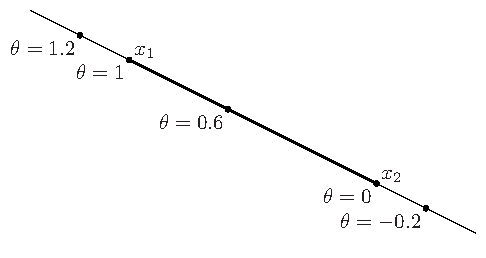
\includegraphics[width=.62\textwidth]{figures/ch02-figure-1.pdf}
\caption*{图2.1\quad 经过 $x_1$ 和 $x_2$ 的直线可参数化为 $\theta x_1+(1-\theta)x_2$，其中 $\theta$ 遍历 $\R$。两点之间的线段对应 $0\le\theta\le1$，图中以深色表示。}
\end{figure}
如果 $C$ 是仿射集，且 $x_0\in C$，那么集合
\[
 V=C-x_0=\{x-x_0\mid x\in C\}
\]
是一个子空间，即对加法与标量乘法封闭。为此，设 $v_1,v_2\in V$，$\alpha,\beta\in\R$。于是 $v_1+x_0\in C$、$v_2+x_0\in C$，从而
\[
 \alpha v_1+\beta v_2+x_0
 =\alpha(v_1+x_0)+\beta(v_2+x_0)+(1-\alpha-\beta)x_0\in C,
\]
因为 $C$ 是仿射集，且 $\alpha+\beta+(1-\alpha-\beta)=1$。由 $\alpha v_1+\beta v_2+x_0\in C$，得到 $\alpha v_1+\beta v_2\in V$。

因此，仿射集 $C$ 可以写成
\[
 C=V+x_0=\{v+x_0\mid v\in V\},
\]
即一个子空间加一个平移量。与仿射集 $C$ 关联的子空间 $V$ 不依赖于 $x_0$ 的选择，因此可以取 $C$ 中任意一点作为 $x_0$。我们将仿射集 $C$ 的\emph{维数}定义为子空间 $V=C-x_0$ 的维数，其中 $x_0$ 为 $C$ 中任意元素。

\begin{origexample}{2.1}
\textbf{线性方程的解集。}线性方程组的解集 $C=\{x\mid Ax=b\}$ 是仿射集，其中 $A\in\R^{m\times n}$、$b\in\R^m$。为证明这一点，设 $x_1,x_2\in C$，即 $Ax_1=b$、$Ax_2=b$。那么对任意 $\theta$，有
\[
\begin{aligned}
 A(\theta x_1+(1-\theta)x_2)
 &=\theta Ax_1+(1-\theta)Ax_2\\
 &=\theta b+(1-\theta)b\\
 &=b.
\end{aligned}
\]
这表明仿射组合 $\theta x_1+(1-\theta)x_2$ 也属于 $C$。与仿射集 $C$ 关联的子空间是 $A$ 的零空间。
\end{origexample}
反过来也成立：每个仿射集都可以表示为某个线性方程组的解集。

% Source PDF page 37 (printed p. 23)
集合 $C\subseteq\R^n$ 中各点的所有仿射组合所成的集合，称为 $C$ 的\emph{仿射包}，记为 $\aff C$：
\[
 \aff C=\{\theta_1x_1+\cdots+\theta_kx_k\mid
 x_1,\ldots,x_k\in C,\ \theta_1+\cdots+\theta_k=1\}.
\]
仿射包是包含 $C$ 的最小仿射集，具体地说：若 $S$ 是满足 $C\subseteq S$ 的任意仿射集，则 $\aff C\subseteq S$。

\subsection{仿射维数与相对内部}
集合 $C$ 的\emph{仿射维数}定义为其仿射包的维数。仿射维数在凸分析和优化中很有用，但不总与其他维数定义一致。例如，考虑 $\R^2$ 中的单位圆周 $\{x\in\R^2\mid x_1^2+x_2^2=1\}$。其仿射包为整个 $\R^2$，故仿射维数为二；但按照大多数维数定义，$\R^2$ 中的单位圆周维数为一。

如果 $C\subseteq\R^n$ 的仿射维数小于 $n$，它便位于仿射集 $\aff C\ne\R^n$ 中。集合 $C$ 的\emph{相对内部}记为 $\relint C$，定义为它相对于 $\aff C$ 的内部：
\[
 \relint C=\{x\in C\mid \text{存在 }r>0, B(x,r)\cap\aff C\subseteq C\},
\]
其中 $B(x,r)=\{y\mid\norm{y-x}\le r\}$ 是关于范数 $\norm{\cdot}$、以 $x$ 为中心、半径为 $r$ 的球。（这里可以使用任意范数，所有范数确定相同的相对内部。）进而可将 $C$ 的\emph{相对边界}定义为 $\cl C\setminus\relint C$，其中 $\cl C$ 是 $C$ 的闭包。

\begin{origexample}{2.2}
考虑 $\R^3$ 的 $(x_1,x_2)$ 平面内的正方形
\[
 C=\{x\in\R^3\mid-1\le x_1\le1,\ -1\le x_2\le1,\ x_3=0\}.
\]
其仿射包为 $(x_1,x_2)$ 平面，即 $\aff C=\{x\in\R^3\mid x_3=0\}$。$C$ 的内部为空，但相对内部为
\[
 \relint C=\{x\in\R^3\mid-1<x_1<1,\ -1<x_2<1,\ x_3=0\}.
\]
它在 $\R^3$ 中的边界是自身；相对边界则是正方形的线框轮廓
\[
 \{x\in\R^3\mid\max\{\abs{x_1},\abs{x_2}\}=1,\ x_3=0\}.
\]
\end{origexample}

\subsection{凸集}
如果 $C$ 中任意两点之间的线段都在 $C$ 中，就称集合 $C$ 是\emph{凸的}。也就是说，对任意 $x_1,x_2\in C$ 以及满足 $0\le\theta\le1$ 的任意 $\theta$，都有
\[
 \theta x_1+(1-\theta)x_2\in C.
\]

% Source PDF page 38 (printed p. 24)
\begin{figure}[htbp]\centering
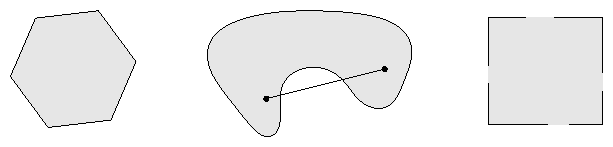
\includegraphics[width=.85\textwidth]{figures/ch02-figure-2.pdf}
\caption*{图2.2\quad 几个简单的凸集与非凸集。左：包含边界（深色线）的六边形是凸集。中：肾形集合不是凸集，因为图中以实点表示的两点之间的线段没有完全包含在集合中。右：正方形包含一部分边界点而不包含另一些边界点，该集合不是凸集。}
\end{figure}
\begin{figure}[htbp]\centering
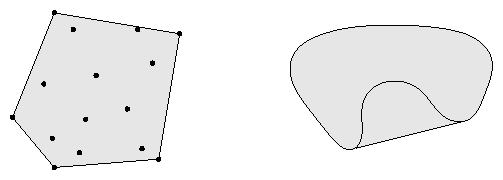
\includegraphics[width=.82\textwidth]{figures/ch02-figure-3.pdf}
\caption*{图2.3\quad $\R^2$ 中两个集合的凸包。左：十五个点（实点）组成的集合，其凸包为阴影所示的五边形。右：图2.2中肾形集合的凸包，为阴影所示的集合。}
\end{figure}
粗略地说，如果集合中任意两点都能沿其间一条没有障碍的直线路径彼此看见，这个集合就是凸的；这里“没有障碍”是指路径始终在集合中。每个仿射集都是凸集，因为它包含任意两个不同点之间的整条直线，当然也包含两点之间的线段。图2.2给出 $\R^2$ 中几个简单的凸集和非凸集。

形如 $\theta_1x_1+\cdots+\theta_kx_k$，且满足 $\theta_1+\cdots+\theta_k=1$、$\theta_i\ge0$（$i=1,\ldots,k$）的点，称为 $x_1,\ldots,x_k$ 的\emph{凸组合}。与仿射集类似，可以证明：一个集合是凸集，当且仅当它包含其中各点的任意凸组合。点的凸组合可理解为这些点的混合或加权平均，$\theta_i$ 表示 $x_i$ 在混合中所占的比例。

集合 $C$ 的\emph{凸包}记作 $\conv C$，是 $C$ 中各点的所有凸组合构成的集合：
\[
 \conv C=\{\theta_1x_1+\cdots+\theta_kx_k\mid
 x_i\in C,\ \theta_i\ge0,\ i=1,\ldots,k,\ \theta_1+\cdots+\theta_k=1\}.
\]
顾名思义，凸包 $\conv C$ 总是凸集。它是包含 $C$ 的最小凸集：若 $B$ 是任意包含 $C$ 的凸集，则 $\conv C\subseteq B$。图2.3说明了凸包的定义。

凸组合的概念可推广至无穷级数、积分，以及最一般的概率分布形式。

% Source PDF page 39 (printed p. 25)
设 $\theta_1,\theta_2,\ldots$ 满足
\[
 \theta_i\ge0,\quad i=1,2,\ldots,\qquad \sum_{i=1}^{\infty}\theta_i=1,
\]
且 $x_1,x_2,\ldots\in C$，其中 $C\subseteq\R^n$ 凸。如果级数收敛，则
\[
 \sum_{i=1}^{\infty}\theta_i x_i\in C.
\]
更一般地，设 $p:\R^n\to\R$ 对所有 $x\in C$ 满足 $p(x)\ge0$，且 $\int_Cp(x)\,\mathrm dx=1$，其中 $C\subseteq\R^n$ 凸。如果积分存在，则
\[
 \int_C p(x)x\,\mathrm dx\in C.
\]
最一般的形式如下：设 $C\subseteq\R^n$ 凸，随机向量 $x$ 以概率一属于 $C$，则 $\E x\in C$。事实上，其他形式都包含在这一形式中。例如，设随机变量 $x$ 只取 $x_1$ 和 $x_2$ 两个值，且 $\Prob(x=x_1)=\theta$、$\Prob(x=x_2)=1-\theta$，其中 $0\le\theta\le1$。那么 $\E x=\theta x_1+(1-\theta)x_2$，又回到了简单的两点凸组合。

\subsection{锥}
若对每个 $x\in C$ 和 $\theta\ge0$ 都有 $\theta x\in C$，就称集合 $C$ 为\emph{锥}，或称其\emph{非负齐次}。若 $C$ 既是凸集又是锥，就称其为\emph{凸锥}；也就是说，对任意 $x_1,x_2\in C$ 和 $\theta_1,\theta_2\ge0$，有
\[
 \theta_1x_1+\theta_2x_2\in C.
\]
从几何上看，这种形式的点构成一个二维扇形，顶点在原点，两条边分别经过 $x_1$ 和 $x_2$，见图2.4。

形如 $\theta_1x_1+\cdots+\theta_kx_k$，且 $\theta_1,\ldots,\theta_k\ge0$ 的点，称为 $x_1,\ldots,x_k$ 的\emph{锥组合}或\emph{非负线性组合}。若 $x_i$ 属于凸锥 $C$，则它们的任意锥组合都在 $C$ 中。反过来，集合 $C$ 是凸锥，当且仅当它包含其元素的所有锥组合。与凸组合、仿射组合一样，锥组合也可推广至无穷级数与积分。

集合 $C$ 的\emph{锥包}是 $C$ 中各点的所有锥组合构成的集合，即
\[
 \{\theta_1x_1+\cdots+\theta_kx_k\mid x_i\in C,\ \theta_i\ge0,\ i=1,\ldots,k\}.
\]
它也是包含 $C$ 的最小凸锥，见图2.5。

% Source PDF page 40 (printed p. 26)
\begin{figure}[htbp]\centering
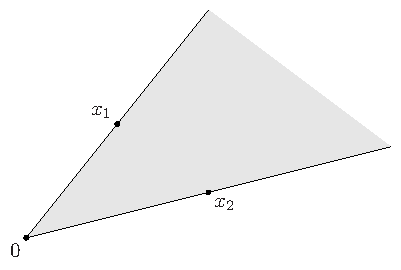
\includegraphics[width=.62\textwidth]{figures/ch02-figure-4.pdf}
\caption*{图2.4\quad 扇形表示所有形如 $\theta_1x_1+\theta_2x_2$、$\theta_1,\theta_2\ge0$ 的点。顶点在原点，对应 $\theta_1=\theta_2=0$；两条边分别对应 $\theta_1=0$ 或 $\theta_2=0$，经过 $x_1$ 和 $x_2$。}
\end{figure}
\begin{figure}[htbp]\centering
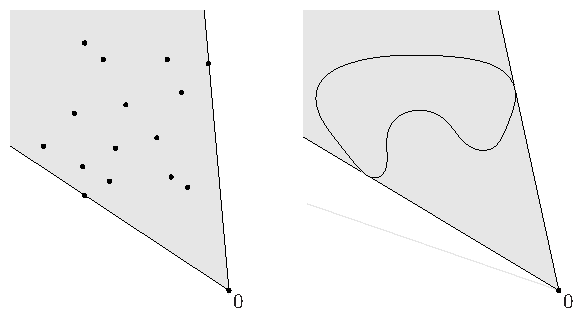
\includegraphics[width=.82\textwidth]{figures/ch02-figure-5.pdf}
\caption*{图2.5\quad 图2.3中两个集合的锥包，以阴影表示。}
\end{figure}

% Source PDF page 41 (printed p. 27)
\section{一些重要例子}
本节介绍一些重要的凸集例子，它们将在本书后续部分反复出现。先从几个简单例子开始。
\begin{itemize}
\item 空集 $\varnothing$、任意单点集 $\{x_0\}$ 以及整个空间 $\R^n$，都是 $\R^n$ 的仿射子集，因此也是凸子集。
\item 任意直线都是仿射集。如果经过原点，它还是子空间，因此也是凸锥。
\item 线段是凸集，但不是仿射集，除非退化为一个点。
\item 形如 $\{x_0+\theta v\mid\theta\ge0\}$、$v\ne0$ 的射线是凸集，但不是仿射集。如果基点 $x_0=0$，它是凸锥。
\item 任意子空间都是仿射集，也是凸锥，因此是凸集。
\end{itemize}

\subsection{超平面与半空间}
\emph{超平面}是形如
\[
 \{x\mid a^{\T}x=b\}
\]
的集合，其中 $a\in\R^n$、$a\ne0$、$b\in\R$。从解析角度看，它是关于 $x$ 各分量的一个非平凡线性方程的解集，因而是仿射集。从几何角度看，超平面 $\{x\mid a^{\T}x=b\}$ 可解释为与给定向量 $a$ 的内积为常数的点集，也可看作法向量为 $a$ 的超平面；常数 $b\in\R$ 确定超平面相对原点的偏移。将超平面写成
\[
 \{x\mid a^{\T}(x-x_0)=0\},
\]
便可理解这一几何解释，其中 $x_0$ 是超平面上任意一点，即满足 $a^{\T}x_0=b$ 的任意点。这个表示还可写成
\[
 \{x\mid a^{\T}(x-x_0)=0\}=x_0+a^{\perp},
\]
其中 $a^{\perp}$ 表示 $a$ 的正交补，即与它正交的所有向量构成的集合：
\[
 a^{\perp}=\{v\mid a^{\T}v=0\}.
\]
这表明，超平面由偏移量 $x_0$ 加上所有与法向量 $a$ 正交的向量构成。图2.6说明了这些几何解释。

一个超平面将 $\R^n$ 分成两个\emph{半空间}。闭半空间是形如
\begin{equation}
 \{x\mid a^{\T}x\le b\}\tag{2.1}
\end{equation}
的集合，其中 $a\ne0$，也就是一个非平凡线性不等式的解集。半空间是凸集，但不是仿射集，见图2.7。

% Source PDF page 42 (printed p. 28)
\begin{figure}[htbp]\centering
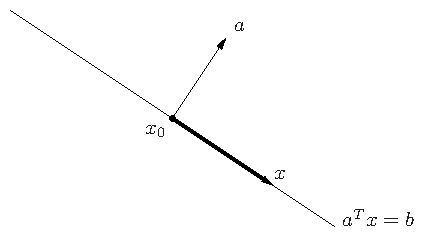
\includegraphics[width=.58\textwidth]{figures/ch02-figure-6.pdf}
\caption*{图2.6\quad $\R^2$ 中的超平面，法向量为 $a$，$x_0$ 为超平面上一点。对超平面上任意点 $x$，向量 $x-x_0$（深色箭头）都与 $a$ 正交。}
\end{figure}
\begin{figure}[htbp]\centering
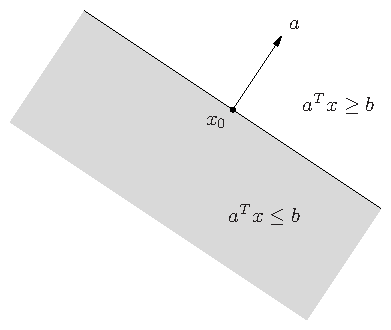
\includegraphics[width=.58\textwidth]{figures/ch02-figure-7.pdf}
\caption*{图2.7\quad $\R^2$ 中由 $a^{\T}x=b$ 定义的超平面确定两个半空间。$a^{\T}x\ge b$ 确定的半空间（无阴影）沿 $a$ 方向延伸；$a^{\T}x\le b$ 确定的半空间（阴影）沿 $-a$ 方向延伸，向量 $a$ 是这个半空间的外法向量。}
\end{figure}

% Source PDF page 43 (printed p. 29)
\begin{figure}[htbp]\centering
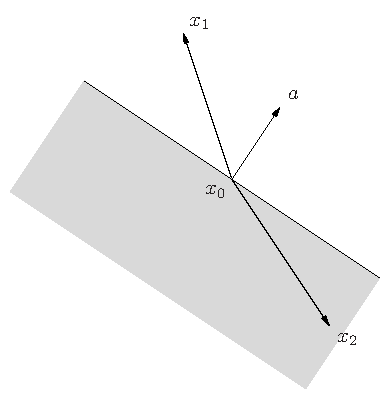
\includegraphics[width=.62\textwidth]{figures/ch02-figure-8.pdf}
\caption*{图2.8\quad 阴影集合是 $a^{\T}(x-x_0)\le0$ 确定的半空间。向量 $x_1-x_0$ 与 $a$ 的夹角为锐角，所以 $x_1$ 不在半空间中；向量 $x_2-x_0$ 与 $a$ 的夹角为钝角，所以 $x_2$ 在半空间中。}
\end{figure}
半空间（2.1）还可表示为
\begin{equation}
 \{x\mid a^{\T}(x-x_0)\le0\},\tag{2.2}
\end{equation}
其中 $x_0$ 是相应超平面上的任意一点，即满足 $a^{\T}x_0=b$。表示（2.2）给出一个简单的几何解释：半空间由 $x_0$ 加上所有与外法向量 $a$ 成钝角或直角的向量构成，如图2.8所示。

半空间（2.1）的边界是超平面 $\{x\mid a^{\T}x=b\}$。集合 $\{x\mid a^{\T}x<b\}$ 是半空间 $\{x\mid a^{\T}x\le b\}$ 的内部，称为\emph{开半空间}。

\subsection{欧几里得球与椭球}
$\R^n$ 中的\emph{欧几里得球}，简称\emph{球}，具有形式
\[
 B(x_c,r)=\{x\mid\norm{x-x_c}_2\le r\}
 =\{x\mid(x-x_c)^{\T}(x-x_c)\le r^2\},
\]
其中 $r>0$，$\norm{\cdot}_2$ 表示欧几里得范数，即 $\norm u_2=(u^{\T}u)^{1/2}$。向量 $x_c$ 是球心，标量 $r$ 是半径；$B(x_c,r)$ 包含距球心 $x_c$ 不超过 $r$ 的所有点。欧几里得球的另一种常见表示为
\[
 B(x_c,r)=\{x_c+ru\mid\norm u_2\le1\}.
\]

% Source PDF page 44 (printed p. 30)
\begin{figure}[htbp]\centering
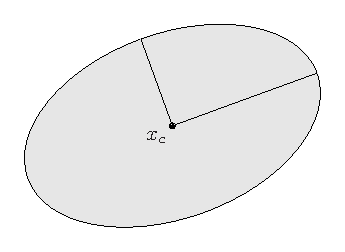
\includegraphics[width=.58\textwidth]{figures/ch02-figure-9.pdf}
\caption*{图2.9\quad $\R^2$ 中的椭球，以阴影表示。中心 $x_c$ 以实点表示，两条半轴以线段表示。}
\end{figure}
欧几里得球是凸集：若 $\norm{x_1-x_c}_2\le r$、$\norm{x_2-x_c}_2\le r$，且 $0\le\theta\le1$，则
\[
\begin{aligned}
 \norm{\theta x_1+(1-\theta)x_2-x_c}_2
 &=\norm{\theta(x_1-x_c)+(1-\theta)(x_2-x_c)}_2\\
 &\le\theta\norm{x_1-x_c}_2+(1-\theta)\norm{x_2-x_c}_2\\
 &\le r.
\end{aligned}
\]
这里使用了 $\norm{\cdot}_2$ 的齐次性和三角不等式，见第A.1.2节。与球相关的另一族凸集是\emph{椭球}，其形式为
\begin{equation}
 \mathcal E=\{x\mid(x-x_c)^{\T}P^{-1}(x-x_c)\le1\},\tag{2.3}
\end{equation}
其中 $P=P^{\T}\succ0$，即 $P$ 对称正定。向量 $x_c\in\R^n$ 是椭球中心，矩阵 $P$ 确定椭球从 $x_c$ 沿各方向延伸的程度；椭球 $\mathcal E$ 的半轴长度为 $\sqrt{\lambda_i}$，其中 $\lambda_i$ 是 $P$ 的特征值。球是 $P=r^2I$ 的椭球。图2.9给出 $\R^2$ 中的一个椭球。

椭球的另一种常见表示是
\begin{equation}
 \mathcal E=\{x_c+Au\mid\norm u_2\le1\},\tag{2.4}
\end{equation}
其中 $A$ 是非奇异方阵。在这个表示中，不失一般性，可以假设 $A$ 对称正定。取 $A=P^{1/2}$，便得到（2.3）定义的椭球。如果（2.4）中的 $A$ 对称半正定但奇异，则（2.4）所示集合称为\emph{退化椭球}；其仿射维数等于 $A$ 的秩。退化椭球也为凸集。

\subsection{范数球与范数锥}
设 $\norm{\cdot}$ 是 $\R^n$ 上的任意范数，见第A.1.2节。由范数的一般性质可证明，以 $x_c$ 为中心、$r$ 为半径的范数球 $\{x\mid\norm{x-x_c}\le r\}$ 是凸集。与范数 $\norm{\cdot}$ 关联的\emph{范数锥}为
\[
 C=\{(x,t)\mid\norm x\le t\}\subseteq\R^{n+1}.
\]

% Source PDF page 45 (printed p. 31)
\begin{figure}[htbp]\centering
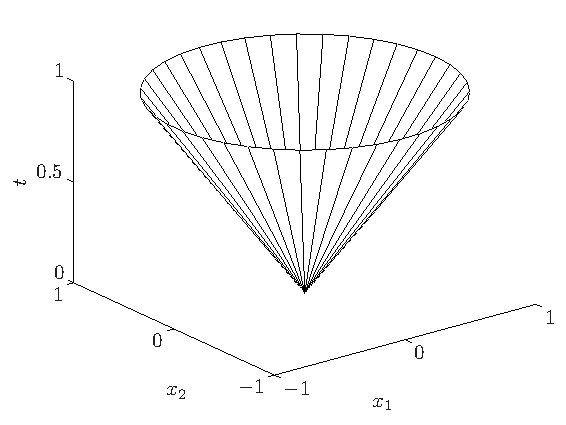
\includegraphics[width=.70\textwidth]{figures/ch02-figure-10.pdf}
\caption*{图2.10\quad $\R^3$ 中二阶锥 $\{(x_1,x_2,t)\mid(x_1^2+x_2^2)^{1/2}\le t\}$ 的边界。}
\end{figure}
顾名思义，范数锥是一个凸锥。

\begin{origexample}{2.3}
\emph{二阶锥}是欧几里得范数对应的范数锥，即
\[
\begin{aligned}
 C&=\{(x,t)\in\R^{n+1}\mid\norm x_2\le t\}\\
 &=\left\{\begin{bmatrix}x\\t\end{bmatrix}\ \middle|\
 \begin{bmatrix}x\\t\end{bmatrix}^{\T}
 \begin{bmatrix}I&0\\0&-1\end{bmatrix}
 \begin{bmatrix}x\\t\end{bmatrix}\le0,\ t\ge0\right\}.
\end{aligned}
\]
二阶锥还有其他几个名称。由于它由二次不等式定义，也称\emph{二次锥}；还称为\emph{Lorentz锥}或\emph{冰淇淋锥}。图2.10给出 $\R^3$ 中的二阶锥。
\end{origexample}

\subsection{多面体}
\emph{多面体}定义为有限个线性等式和线性不等式的解集：
\begin{equation}
 \mathcal P=\{x\mid a_j^{\T}x\le b_j,\ j=1,\ldots,m,
 \ c_j^{\T}x=d_j,\ j=1,\ldots,p\}.\tag{2.5}
\end{equation}
因此，多面体是有限个半空间和超平面的交。仿射集，例如子空间、超平面、直线，以及射线、线段、半空间，都是多面体。容易证明多面体为凸集。有界多面体有时称为多胞体，但有些作者使用相反的约定：将所有（2.5）形式的集合称为多胞体，将其中有界的集合称为多面体。图2.11是五个半空间相交形成的多面体。

% Source PDF page 46 (printed p. 32)
\begin{figure}[htbp]\centering
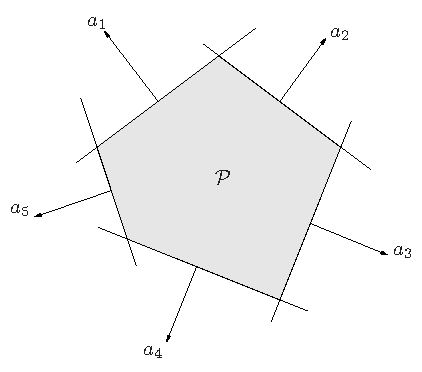
\includegraphics[width=.60\textwidth]{figures/ch02-figure-11.pdf}
\caption*{图2.11\quad 多面体 $\mathcal P$（阴影）是五个半空间的交，外法向量分别为 $a_1,\ldots,a_5$。}
\end{figure}
将（2.5）写成紧凑形式会更方便：
\begin{equation}
 \mathcal P=\{x\mid Ax\preceq b,\ Cx=d\},\tag{2.6}
\end{equation}
其中
\[
 A=\begin{bmatrix}a_1^{\T}\\\vdots\\a_m^{\T}\end{bmatrix},
 \qquad C=\begin{bmatrix}c_1^{\T}\\\vdots\\c_p^{\T}\end{bmatrix}.
\]
符号 $\preceq$ 表示 $\R^m$ 中的向量不等式或逐分量不等式：$u\preceq v$ 的意思是，对 $i=1,\ldots,m$，都有 $u_i\le v_i$。

\begin{origexample}{2.4}
\emph{非负正交锥}是各分量非负的点所成的集合，即
\[
 \R_+^n=\{x\in\R^n\mid x_i\ge0,\ i=1,\ldots,n\}
 =\{x\in\R^n\mid x\succeq0\}.
\]
这里 $\R_+$ 表示非负数集，即 $\R_+=\{x\in\R\mid x\ge0\}$。非负正交锥既是多面体又是锥，因此称为\emph{多面锥}。
\end{origexample}

\subsubsection*{单纯形}
单纯形是另一族重要的多面体。设 $k+1$ 个点 $v_0,\ldots,v_k\in\R^n$ 仿射无关，即 $v_1-v_0,\ldots,v_k-v_0$ 线性无关。由这些点确定的\emph{单纯形}为
\begin{equation}
 C=\conv\{v_0,\ldots,v_k\}
 =\{\theta_0v_0+\cdots+\theta_kv_k\mid\theta\succeq0,\ \one^{\T}\theta=1\}.\tag{2.7}
\end{equation}

% Source PDF page 47 (printed p. 33)
这里 $\one$ 表示各元素均为一的向量。这个单纯形的仿射维数为 $k$，因此有时称为 $\R^n$ 中的 $k$ 维单纯形。

\begin{origexample}{2.5}
\textbf{几个常见的单纯形。}一维单纯形是线段；二维单纯形是三角形及其内部；三维单纯形是四面体。

\emph{单位单纯形}是由零向量与单位向量 $0,e_1,\ldots,e_n\in\R^n$ 确定的 $n$ 维单纯形。它可表示为满足下式的向量集：
\[
 x\succeq0,\qquad\one^{\T}x\le1.
\]
\emph{概率单纯形}是由单位向量 $e_1,\ldots,e_n\in\R^n$ 确定的 $(n-1)$ 维单纯形，即满足
\[
 x\succeq0,\qquad\one^{\T}x=1
\]
的向量集。概率单纯形中的向量对应含 $n$ 个元素的集合上的概率分布，$x_i$ 解释为第 $i$ 个元素的概率。
\end{origexample}

为把单纯形（2.7）描述为多面体，即写成（2.6）的形式，作如下处理。由定义，$x\in C$ 当且仅当存在 $\theta\succeq0$、$\one^{\T}\theta=1$，使 $x=\theta_0v_0+\theta_1v_1+\cdots+\theta_kv_k$。等价地，令 $y=(\theta_1,\ldots,\theta_k)$，且
\[
 B=\begin{bmatrix}v_1-v_0&\cdots&v_k-v_0\end{bmatrix}\in\R^{n\times k},
\]
则 $x\in C$ 当且仅当存在 $y\succeq0$、$\one^{\T}y\le1$，使
\begin{equation}
 x=v_0+By.\tag{2.8}
\end{equation}
点 $v_0,\ldots,v_k$ 仿射无关，意味着 $B$ 的秩为 $k$。因此，存在非奇异矩阵 $A=(A_1,A_2)\in\R^{n\times n}$，使
\[
 AB=\begin{bmatrix}A_1\\A_2\end{bmatrix}B
 =\begin{bmatrix}I\\0\end{bmatrix}.
\]
将（2.8）左乘 $A$，得到
\[
 A_1x=A_1v_0+y,\qquad A_2x=A_2v_0.
\]
因此，$x\in C$ 当且仅当 $A_2x=A_2v_0$，且向量 $y=A_1x-A_1v_0$ 满足 $y\succeq0$、$\one^{\T}y\le1$。换言之，$x\in C$ 当且仅当
\[
 A_2x=A_2v_0,\qquad A_1x\succeq A_1v_0,\qquad
 \one^{\T}A_1x\le1+\one^{\T}A_1v_0.
\]
这些都是关于 $x$ 的线性等式或不等式，因而描述了一个多面体。

% Source PDF page 48 (printed p. 34)
\subsubsection*{多面体的凸包描述}
有限集合 $\{v_1,\ldots,v_k\}$ 的凸包为
\[
 \conv\{v_1,\ldots,v_k\}
 =\{\theta_1v_1+\cdots+\theta_kv_k\mid\theta\succeq0,\ \one^{\T}\theta=1\}.
\]
该集合是有界多面体，但除了单纯形等特殊情况，将它写成（2.5）的形式，也就是用一组线性等式与不等式表示，并不简单。

这种凸包描述的一个推广是
\begin{equation}
 \{\theta_1v_1+\cdots+\theta_kv_k\mid
 \theta_1+\cdots+\theta_m=1,\ \theta_i\ge0,\ i=1,\ldots,k\},\tag{2.9}
\end{equation}
其中 $m\le k$。这里考虑 $v_i$ 的非负线性组合，但只要求前 $m$ 个系数之和为一。也可以把（2.9）解释为点 $v_1,\ldots,v_m$ 的凸包，加上点 $v_{m+1},\ldots,v_k$ 的锥包。集合（2.9）定义一个多面体；反过来，每个多面体都能写成这种形式，尽管这里不作证明。

多面体的表示方式是一个微妙的问题，对实际计算有重要影响。例如，考虑 $\R^n$ 中 $\ell_\infty$ 范数的单位球
\[
 C=\{x\mid\abs{x_i}\le1,\ i=1,\ldots,n\}.
\]
用（2.5）的形式，可以通过 $2n$ 个线性不等式 $\pm e_i^{\T}x\le1$ 描述 $C$，其中 $e_i$ 是第 $i$ 个单位向量。但要用凸包形式（2.9）描述，至少需要 $2^n$ 个点：
\[
 C=\conv\{v_1,\ldots,v_{2^n}\},
\]
其中 $v_1,\ldots,v_{2^n}$ 是所有分量取值为 $1$ 或 $-1$ 的 $2^n$ 个向量。因此，当 $n$ 很大时，这两种描述的规模相差很大。

\subsection{半正定锥}
用 $\mathbf S^n$ 表示对称 $n\times n$ 矩阵集，
\[
 \mathbf S^n=\{X\in\R^{n\times n}\mid X=X^{\T}\},
\]
它是维数为 $n(n+1)/2$ 的向量空间。用 $\mathbf S_+^n$ 表示对称半正定矩阵集，
\[
 \mathbf S_+^n=\{X\in\mathbf S^n\mid X\succeq0\},
\]
用 $\mathbf S_{++}^n$ 表示对称正定矩阵集，
\[
 \mathbf S_{++}^n=\{X\in\mathbf S^n\mid X\succ0\}.
\]
这组记号意在与表示非负实数的 $\R_+$、表示正实数的 $\R_{++}$ 类比。

% Source PDF page 49 (printed p. 35)
\begin{figure}[htbp]\centering
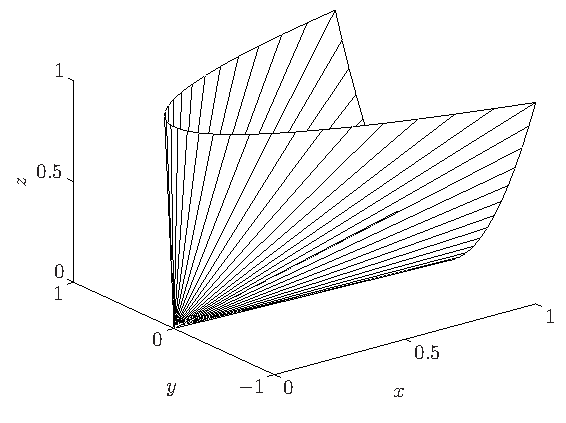
\includegraphics[width=.70\textwidth]{figures/ch02-figure-12.pdf}
\caption*{图2.12\quad $\mathbf S^2$ 中半正定锥的边界。}
\end{figure}
集合 $\mathbf S_+^n$ 是凸锥：如果 $\theta_1,\theta_2\ge0$，且 $A,B\in\mathbf S_+^n$，则 $\theta_1A+\theta_2B\in\mathbf S_+^n$。这可由半正定性的定义直接得到：对任意 $x\in\R^n$，若 $A\succeq0$、$B\succeq0$ 且 $\theta_1,\theta_2\ge0$，则
\[
 x^{\T}(\theta_1A+\theta_2B)x
 =\theta_1x^{\T}Ax+\theta_2x^{\T}Bx\ge0.
\]

\begin{origexample}{2.6}
\textbf{$\mathbf S^2$ 中的半正定锥。}有
\[
 X=\begin{bmatrix}x&y\\y&z\end{bmatrix}\in\mathbf S_+^2
 \quad\Longleftrightarrow\quad x\ge0,\quad z\ge0,\quad xz\ge y^2.
\]
图2.12将 $(x,y,z)$ 画在 $\R^3$ 中，展示了这个锥的边界。
\end{origexample}

\section{保持凸性的运算}
本节介绍一些保持集合凸性的运算，以及由已有凸集构造新凸集的运算。这些运算与第2.2节中的简单例子一起，构成一套凸集运算规则，可用于判断或证明集合的凸性。

% Source PDF page 50 (printed p. 36)
\subsection{交集}
交运算保持凸性：如果 $S_1$ 和 $S_2$ 凸，那么 $S_1\cap S_2$ 凸。该性质可推广到无穷多个集合的交：若对每个 $\alpha\in\mathcal A$，$S_\alpha$ 都凸，则 $\bigcap_{\alpha\in\mathcal A}S_\alpha$ 凸。子空间、仿射集和凸锥也都对任意交运算封闭。一个简单例子是，多面体为半空间和超平面的交，而后者均凸，因此多面体凸。

\begin{origexample}{2.7}
半正定锥 $\mathbf S_+^n$ 可写成
\[
 \bigcap_{z\ne0}\{X\in\mathbf S^n\mid z^{\T}Xz\ge0\}.
\]
对每个 $z\ne0$，$z^{\T}Xz$ 是 $X$ 的一个不恒为零的线性函数，因此集合
\[
 \{X\in\mathbf S^n\mid z^{\T}Xz\ge0\}
\]
实际上是 $\mathbf S^n$ 中的半空间。半正定锥是无穷多个半空间的交，所以凸。
\end{origexample}

\begin{origexample}{2.8}
考虑集合
\begin{equation}
 S=\{x\in\R^m\mid\abs{p(t)}\le1,\ \abs t\le\pi/3\},\tag{2.10}
\end{equation}
其中 $p(t)=\sum_{k=1}^m x_k\cos kt$。集合 $S$ 可以表示为无穷多个带状区域的交 $S=\bigcap_{\abs t\le\pi/3}S_t$，其中
\[
 S_t=\{x\mid-1\le(\cos t,\ldots,\cos mt)^{\T}x\le1\},
\]
所以凸。图2.13和图2.14展示了 $m=2$ 时的定义及相应集合。
\end{origexample}

上面的例子将集合表示为可能无穷多个半空间的交，从而证明其凸性。第2.5.1节将看到，反过来也成立：每个闭凸集 $S$ 都是若干半空间的交，通常需要无穷多个。事实上，闭凸集 $S$ 等于所有包含它的半空间的交：
\[
 S=\bigcap\{H\mid H\text{ 为半空间},\ S\subseteq H\}.
\]

\subsection{仿射函数}
回顾，函数 $f:\R^n\to\R^m$ 若是线性函数与常数的和，就称为仿射函数，也就是具有形式 $f(x)=Ax+b$，其中 $A\in\R^{m\times n}$、$b\in\R^m$。若 $S\subseteq\R^n$ 凸，$f:\R^n\to\R^m$ 仿射，则 $S$ 在 $f$ 下的像
\[
 f(S)=\{f(x)\mid x\in S\}
\]
为凸集。

% Source PDF page 51 (printed p. 37)
\begin{figure}[htbp]\centering
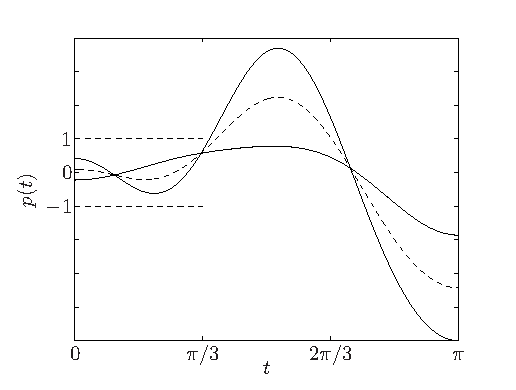
\includegraphics[width=.72\textwidth]{figures/ch02-figure-13.pdf}
\caption*{图2.13\quad （2.10）中 $m=2$ 时，与集合 $S$ 中三个点相应的三角多项式。虚线表示的三角多项式是另外两个的平均。}
\end{figure}
\begin{figure}[htbp]\centering
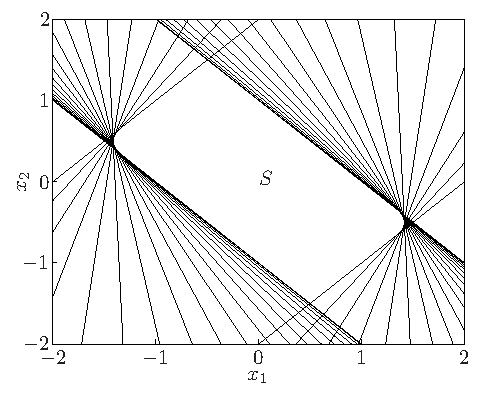
\includegraphics[width=.63\textwidth]{figures/ch02-figure-14.pdf}
\caption*{图2.14\quad （2.10）中 $m=2$ 时的集合 $S$，为图中央的白色区域。它是无穷多个带状区域的交，图中画出了其中20个，因此为凸集。}
\end{figure}

% Source PDF page 52 (printed p. 38)
类似地，若 $f:\R^k\to\R^n$ 仿射，则 $S$ 在 $f$ 下的逆像
\[
 f^{-1}(S)=\{x\mid f(x)\in S\}
\]
也凸。

两个简单例子是缩放和平移。若 $S\subseteq\R^n$ 凸，$\alpha\in\R$、$a\in\R^n$，则 $\alpha S$ 和 $S+a$ 都凸，其中
\[
 \alpha S=\{\alpha x\mid x\in S\},\qquad S+a=\{x+a\mid x\in S\}.
\]
凸集投影到部分坐标所得的集合也凸：若 $S\subseteq\R^m\times\R^n$ 凸，则
\[
 T=\{x_1\in\R^m\mid\text{存在 }x_2\in\R^n,\ (x_1,x_2)\in S\}
\]
凸。

两个集合的\emph{和}定义为
\[
 S_1+S_2=\{x+y\mid x\in S_1,\ y\in S_2\}.
\]
若 $S_1$ 和 $S_2$ 凸，则 $S_1+S_2$ 凸。因为当 $S_1$ 和 $S_2$ 凸时，它们的直积或笛卡尔积
\[
 S_1\times S_2=\{(x_1,x_2)\mid x_1\in S_1,\ x_2\in S_2\}
\]
也凸，而该集合在线性函数 $f(x_1,x_2)=x_1+x_2$ 下的像，正是 $S_1+S_2$。

还可以考虑 $S_1,S_2\in\R^n\times\R^m$ 的\emph{部分和}，定义为
\[
 S=\{(x,y_1+y_2)\mid(x,y_1)\in S_1,\ (x,y_2)\in S_2\},
\]
其中 $x\in\R^n$、$y_i\in\R^m$。$m=0$ 时，部分和给出 $S_1$ 和 $S_2$ 的交；$n=0$ 时，它就是集合加法。凸集的部分和仍凸，见习题2.16。

\begin{origexample}{2.9}
\textbf{多面体。}多面体 $\{x\mid Ax\preceq b,\ Cx=d\}$ 可写成非负正交锥与原点的笛卡尔积在仿射函数 $f(x)=(b-Ax,d-Cx)$ 下的逆像：
\[
 \{x\mid Ax\preceq b,\ Cx=d\}
 =\{x\mid f(x)\in\R_+^m\times\{0\}\}.
\]
\end{origexample}

\begin{origexample}{2.10}
\textbf{线性矩阵不等式的解集。}条件
\begin{equation}
 A(x)=x_1A_1+\cdots+x_nA_n\preceq B,\tag{2.11}
\end{equation}
其中 $B,A_i\in\mathbf S^m$，称为关于 $x$ 的\emph{线性矩阵不等式}（LMI）。注意，它与普通线性不等式
\[
 a^{\T}x=x_1a_1+\cdots+x_na_n\le b
\]
类似，后者的 $b,a_i\in\R$。

线性矩阵不等式的解集 $\{x\mid A(x)\preceq B\}$ 是凸集。事实上，它是半正定锥在仿射函数 $f:\R^n\to\mathbf S^m$，$f(x)=B-A(x)$ 下的逆像。
\end{origexample}

% Source PDF page 53 (printed p. 39)
\begin{origexample}{2.11}
\textbf{双曲锥。}集合
\[
 \{x\mid x^{\T}Px\le(c^{\T}x)^2,\ c^{\T}x\ge0\},
\]
其中 $P\in\mathbf S_+^n$、$c\in\R^n$，为凸集，因为它是二阶锥
\[
 \{(z,t)\mid z^{\T}z\le t^2,\ t\ge0\}
\]
在仿射函数 $f(x)=(P^{1/2}x,c^{\T}x)$ 下的逆像。
\end{origexample}

\begin{origexample}{2.12}
\textbf{椭球。}椭球
\[
 \mathcal E=\{x\mid(x-x_c)^{\T}P^{-1}(x-x_c)\le1\},
\]
其中 $P\in\mathbf S_{++}^n$，是单位欧几里得球 $\{u\mid\norm u_2\le1\}$ 在仿射映射 $f(u)=P^{1/2}u+x_c$ 下的像。它也是单位球在仿射映射 $g(x)=P^{-1/2}(x-x_c)$ 下的逆像。
\end{origexample}

\subsection{线性分式函数与透视函数}
本节研究一类比仿射函数更一般、但仍保持凸性的函数，称为\emph{线性分式函数}。

\subsubsection*{透视函数}
定义\emph{透视函数} $P:\R^{n+1}\to\R^n$，其定义域为 $\dom P=\R^n\times\R_{++}$，函数值为 $P(z,t)=z/t$。这里 $\R_{++}=\{x\in\R\mid x>0\}$ 为正数集。透视函数缩放或归一化向量，使最后一个分量等于一，再去掉最后一个分量。

\begin{quote}\textbf{说明2.1}\quad
可以把透视函数理解为针孔相机的作用。$\R^3$ 中的针孔相机由不透光水平面 $x_3=0$ 构成，原点处有一个允许光线通过的针孔，水平像平面为 $x_3=-1$。相机上方，即 $x_3>0$ 处，位于 $x$ 的物体，在像平面上的点 $-(x_1/x_3,x_2/x_3,1)$ 处成像。去掉恒为 $-1$ 的最后一个分量，物体 $x$ 的像在像平面上的位置就是 $y=-(x_1/x_3,x_2/x_3)=-P(x)$，见图2.15。
\end{quote}
若 $C\subseteq\dom P$ 凸，则其像
\[
 P(C)=\{P(x)\mid x\in C\}
\]
也凸。这个结果符合直觉：通过针孔相机观察凸物体，会得到凸的像。为证明这一点，我们说明透视函数将线段映射为线段。这也符合直觉：通过针孔相机观察线段，得到的像仍是线段。

% Source PDF page 54 (printed p. 40)
\begin{figure}[htbp]\centering
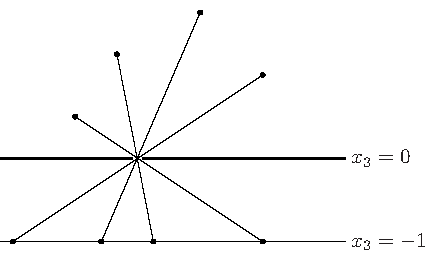
\includegraphics[width=.65\textwidth]{figures/ch02-figure-15.pdf}
\caption*{图2.15\quad 透视函数的针孔相机解释。深色水平线表示 $\R^3$ 中不透光的平面 $x_3=0$，只在原点有针孔。平面上方的物体或光源在较浅水平线表示的像平面 $x_3=-1$ 上成像。光源位置到像位置的映射与透视函数有关。}
\end{figure}
设 $x=(\widetilde x,x_{n+1})$、$y=(\widetilde y,y_{n+1})\in\R^{n+1}$，且 $x_{n+1}>0$、$y_{n+1}>0$。对 $0\le\theta\le1$，有
\[
 P(\theta x+(1-\theta)y)
 =\frac{\theta\widetilde x+(1-\theta)\widetilde y}
 {\theta x_{n+1}+(1-\theta)y_{n+1}}
 =\mu P(x)+(1-\mu)P(y),
\]
其中
\[
 \mu=\frac{\theta x_{n+1}}
 {\theta x_{n+1}+(1-\theta)y_{n+1}}\in[0,1].
\]
$\theta$ 与 $\mu$ 的对应关系是单调的：当 $\theta$ 在0与1之间变化，遍历线段 $[x,y]$ 时，$\mu$ 也在0与1之间变化，遍历线段 $[P(x),P(y)]$。因此，$P([x,y])=[P(x),P(y)]$。

现在，设 $C$ 凸且 $C\subseteq\dom P$，即对每个 $x\in C$ 都有 $x_{n+1}>0$，并取 $x,y\in C$。为证明 $P(C)$ 凸，只需说明线段 $[P(x),P(y)]$ 在 $P(C)$ 中。该线段是 $[x,y]$ 在 $P$ 下的像，因而确实包含在 $P(C)$ 中。

凸集在透视函数下的逆像也凸：若 $C\subseteq\R^n$ 凸，则
\[
 P^{-1}(C)=\{(x,t)\in\R^{n+1}\mid x/t\in C,\ t>0\}
\]
凸。为证明这一点，设 $(x,t)\in P^{-1}(C)$、$(y,s)\in P^{-1}(C)$，且 $0\le\theta\le1$。需要说明
\[
 \theta(x,t)+(1-\theta)(y,s)\in P^{-1}(C),
\]
即
\[
 \frac{\theta x+(1-\theta)y}{\theta t+(1-\theta)s}\in C.
\]

% Source PDF page 55 (printed p. 41)
$\theta t+(1-\theta)s>0$ 显然成立。上述结论由下式得到：
\[
 \frac{\theta x+(1-\theta)y}{\theta t+(1-\theta)s}
 =\mu(x/t)+(1-\mu)(y/s),
 \qquad\mu=\frac{\theta t}{\theta t+(1-\theta)s}\in[0,1].
\]

\subsubsection*{线性分式函数}
将透视函数与仿射函数复合，得到\emph{线性分式函数}。设 $g:\R^n\to\R^{m+1}$ 为仿射函数，即
\begin{equation}
 g(x)=\begin{bmatrix}A\\c^{\T}\end{bmatrix}x+
 \begin{bmatrix}b\\d\end{bmatrix},\tag{2.12}
\end{equation}
其中 $A\in\R^{m\times n}$、$b\in\R^m$、$c\in\R^n$、$d\in\R$。由 $f=P\circ g$ 定义的函数 $f:\R^n\to\R^m$，即
\begin{equation}
 f(x)=(Ax+b)/(c^{\T}x+d),\qquad
 \dom f=\{x\mid c^{\T}x+d>0\},\tag{2.13}
\end{equation}
称为\emph{线性分式函数}或\emph{射影函数}。当 $c=0$、$d>0$ 时，$\dom f=\R^n$，且 $f$ 为仿射函数。因此，可以把仿射函数和线性函数视为线性分式函数的特例。

\begin{quote}\textbf{说明2.2\quad 射影解释。}
将线性分式函数表示为矩阵
\begin{equation}
 Q=\begin{bmatrix}A&b\\c^{\T}&d\end{bmatrix}
 \in\R^{(m+1)\times(n+1)}\tag{2.14}
\end{equation}
往往很方便。它作用于，即乘上，形如 $(x,1)$ 的点，得到 $(Ax+b,c^{\T}x+d)$。然后将结果缩放或归一化，使最后一个分量为一，得到 $(f(x),1)$。

这个表示可以通过将 $\R^n$ 与 $\R^{n+1}$ 中的一组射线关联起来，获得几何解释。对每个 $z\in\R^n$，关联 $\R^{n+1}$ 中的开射线 $\mathcal P(z)=\{t(z,1)\mid t>0\}$。该射线的最后一个分量取正值。反过来，$\R^{n+1}$ 中任意以原点为基点、最后一个分量取正值的射线，都能对某个 $v\in\R^n$ 写成 $\mathcal P(v)=\{t(v,1)\mid t\ge0\}$。$\R^n$ 与最后一个分量为正的半空间中各射线之间的这一射影对应 $\mathcal P$，是双射。

线性分式函数（2.13）可写成
\[
 f(x)=\mathcal P^{-1}(Q\mathcal P(x)).
\]
因此，从 $x\in\dom f$，即 $c^{\T}x+d>0$ 出发，先在 $\R^{n+1}$ 中形成射线 $\mathcal P(x)$；矩阵 $Q$ 对应的线性变换将该射线变为另一条射线 $Q\mathcal P(x)$。因为 $x\in\dom f$，新射线的最后一个分量取正值。最后，作逆射影变换得到 $f(x)$。
\end{quote}

% Source PDF page 56 (printed p. 42)
\begin{figure}[htbp]\centering
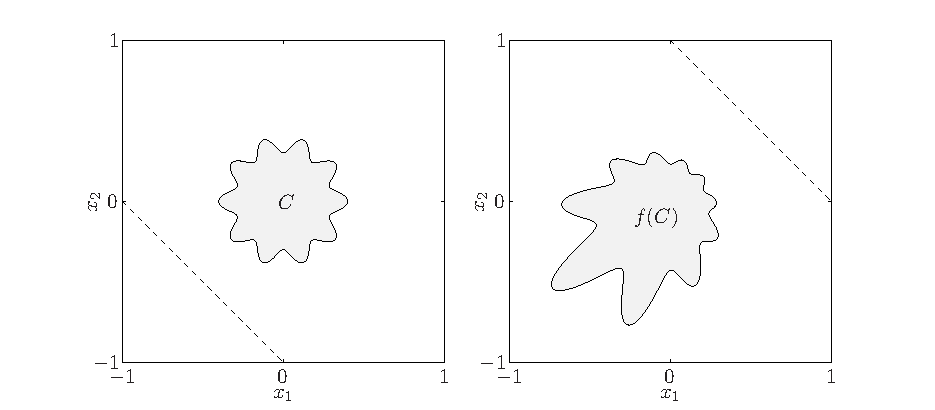
\includegraphics[width=.88\textwidth]{figures/ch02-figure-16.pdf}
\caption*{图2.16\quad 左：集合 $C\subseteq\R^2$。虚线表示线性分式函数 $f(x)=x/(x_1+x_2+1)$ 的定义域边界，其中 $\dom f=\{(x_1,x_2)\mid x_1+x_2+1>0\}$。右：$C$ 在 $f$ 下的像。虚线表示 $f^{-1}$ 的定义域边界。}
\end{figure}
与透视函数一样，线性分式函数保持凸性。如果 $C$ 凸且在 $f$ 的定义域内，即对 $x\in C$ 有 $c^{\T}x+d>0$，则其像 $f(C)$ 凸。这由前面的结果直接得到：$C$ 在仿射映射（2.12）下的像凸，这个像再经透视函数 $P$ 映射得到 $f(C)$，仍凸。类似地，若 $C\subseteq\R^m$ 凸，则逆像 $f^{-1}(C)$ 凸。

\begin{origexample}{2.13}
\textbf{条件概率。}设随机变量 $u$ 和 $v$ 分别取值于 $\{1,\ldots,n\}$ 和 $\{1,\ldots,m\}$，用 $p_{ij}$ 表示 $\Prob(u=i,v=j)$。条件概率 $f_{ij}=\Prob(u=i\mid v=j)$ 为
\[
 f_{ij}=\frac{p_{ij}}{\sum_{k=1}^n p_{kj}}.
\]
因此，$f$ 由 $p$ 经线性分式映射得到。

由此可知，如果 $C$ 是 $(u,v)$ 的联合概率构成的凸集，那么相应的给定 $v$ 时 $u$ 的条件概率集合也凸。
\end{origexample}
图2.16给出集合 $C\subseteq\R^2$ 及其在线性分式函数
\[
 f(x)=\frac1{x_1+x_2+1}x,\qquad
 \dom f=\{(x_1,x_2)\mid x_1+x_2+1>0\}
\]
下的像。

% Source PDF page 57 (printed p. 43)
\section{广义不等式}
\subsection{正常锥与广义不等式}
如果锥 $K\subseteq\R^n$ 满足以下条件，就称其为\emph{正常锥}：
\begin{itemize}
\item $K$ 凸。
\item $K$ 闭。
\item $K$ 是实心的，即内部非空。
\item $K$ 尖，即不包含直线，等价地，$x\in K$、$-x\in K$ 蕴含 $x=0$。
\end{itemize}
正常锥 $K$ 可以用来定义\emph{广义不等式}，它是 $\R^n$ 上的一种偏序，具有 $\R$ 上通常次序的许多性质。与正常锥 $K$ 关联的偏序定义为
\[
 x\preceq_K y\quad\Longleftrightarrow\quad y-x\in K.
\]
也用 $x\succeq_K y$ 表示 $y\preceq_K x$。类似地，定义相应的严格偏序
\[
 x\prec_K y\quad\Longleftrightarrow\quad y-x\in\operatorname{int}K,
\]
用 $x\succ_K y$ 表示 $y\prec_K x$。为区别于严格广义不等式 $\prec_K$，有时将 $\preceq_K$ 称为非严格广义不等式。

当 $K=\R_+$ 时，偏序 $\preceq_K$ 就是 $\R$ 上通常的次序 $\le$，严格偏序 $\prec_K$ 就是通常的严格次序 $<$。因此，广义不等式包含 $\R$ 中普通的非严格与严格不等式这一特例。

\begin{origexample}{2.14}
\textbf{非负正交锥与逐分量不等式。}非负正交锥 $K=\R_+^n$ 是正常锥。相应的广义不等式 $\preceq_K$ 对应向量间的逐分量不等式：$x\preceq_K y$ 表示 $x_i\le y_i$，$i=1,\ldots,n$。相应的严格不等式对应逐分量严格不等式：$x\prec_K y$ 表示 $x_i<y_i$，$i=1,\ldots,n$。

与非负正交锥关联的非严格与严格偏序经常出现，因此省略下标 $\R_+^n$；当符号 $\preceq$ 或 $\prec$ 出现在向量之间时，就按此理解。
\end{origexample}

\begin{origexample}{2.15}
\textbf{半正定锥与矩阵不等式。}半正定锥 $\mathbf S_+^n$ 是 $\mathbf S^n$ 中的正常锥。相应的广义不等式 $\preceq_K$ 就是通常的矩阵不等式：$X\preceq_K Y$ 表示 $Y-X$ 半正定。$\mathbf S_+^n$ 在 $\mathbf S^n$ 中的内部由正定矩阵构成，因此严格广义不等式也与对称矩阵间通常的严格不等式一致：$X\prec_K Y$ 表示 $Y-X$ 正定。

这一偏序也十分常见，因此同样省略下标，对对称矩阵只写 $X\preceq Y$ 或 $X\prec Y$，并理解为相对于半正定锥的广义不等式。
\end{origexample}

% Source PDF page 58 (printed p. 44)
\begin{origexample}{2.16}
\textbf{在 $[0,1]$ 上非负的多项式锥。}定义
\begin{equation}
 K=\{c\in\R^n\mid c_1+c_2t+\cdots+c_nt^{n-1}\ge0,\ t\in[0,1]\}.\tag{2.15}
\end{equation}
即 $K$ 是在区间 $[0,1]$ 上非负的 $n-1$ 次多项式的系数构成的锥。可以证明，$K$ 是正常锥；其内部是在区间 $[0,1]$ 上为正的多项式的系数集。

两个向量 $c,d\in\R^n$ 满足 $c\preceq_K d$，当且仅当对所有 $t\in[0,1]$ 有
\[
 c_1+c_2t+\cdots+c_nt^{n-1}
 \le d_1+d_2t+\cdots+d_nt^{n-1}.
\]
\end{origexample}

\subsubsection*{广义不等式的性质}
广义不等式 $\preceq_K$ 满足许多性质，例如：
\begin{itemize}
\item 加法保持 $\preceq_K$：若 $x\preceq_K y$、$u\preceq_K v$，则 $x+u\preceq_K y+v$。
\item 传递性：若 $x\preceq_K y$、$y\preceq_K z$，则 $x\preceq_K z$。
\item 非负缩放保持 $\preceq_K$：若 $x\preceq_K y$、$\alpha\ge0$，则 $\alpha x\preceq_K\alpha y$。
\item 自反性：$x\preceq_K x$。
\item 反对称性：若 $x\preceq_K y$ 且 $y\preceq_K x$，则 $x=y$。
\item 取极限保持 $\preceq_K$：若对 $i=1,2,\ldots$ 有 $x_i\preceq_K y_i$，且 $i\to\infty$ 时 $x_i\to x$、$y_i\to y$，则 $x\preceq_K y$。
\end{itemize}
相应的严格广义不等式 $\prec_K$ 满足例如以下性质：
\begin{itemize}
\item 若 $x\prec_K y$，则 $x\preceq_K y$。
\item 若 $x\prec_K y$、$u\preceq_K v$，则 $x+u\prec_K y+v$。
\item 若 $x\prec_K y$、$\alpha>0$，则 $\alpha x\prec_K\alpha y$。
\item $x\not\prec_K x$。
\item 若 $x\prec_K y$，则对足够小的 $u$ 和 $v$，有 $x+u\prec_K y+v$。
\end{itemize}
这些性质来自 $\preceq_K$、$\prec_K$ 的定义及正常锥的性质，见习题2.30。

% Source PDF page 59 (printed p. 45)
\subsection{最小元与极小元}
广义不等式的记号 $\preceq_K$、$\prec_K$ 意在提示其与 $\R$ 上普通不等式 $\le$、$<$ 的类比。虽然普通不等式的许多性质对广义不等式成立，但一些重要性质并不成立。最明显的区别是，$\R$ 上的 $\le$ 是全序：任意两点都可比较，即 $x\le y$ 或 $y\le x$ 总有一个成立。其他广义不等式不具备这一性质。一个后果是，最小值与最大值等概念在广义不等式下会更复杂。本节简要讨论这一点。

若 $x\in S$，且对每个 $y\in S$ 都有 $x\preceq_K y$，就称 $x$ 为 $S$ 关于广义不等式 $\preceq_K$ 的\emph{最小元}。类似地，可以定义集合 $S$ 关于广义不等式的\emph{最大元}。如果集合有最小元或最大元，它就是唯一的。另一个相关概念是\emph{极小元}：若 $x\in S$，且 $y\in S$、$y\preceq_K x$ 只有在 $y=x$ 时才成立，就称 $x$ 为 $S$ 关于 $\preceq_K$ 的极小元。\emph{极大元}的定义类似。一个集合可以有许多不同的极小元或极大元。

可用简单的集合记号描述最小元与极小元。点 $x\in S$ 是 $S$ 的最小元，当且仅当
\[
 S\subseteq x+K.
\]
这里 $x+K$ 表示所有能与 $x$ 比较、且按照 $\preceq_K$ 大于或等于 $x$ 的点。点 $x\in S$ 是极小元，当且仅当
\[
 (x-K)\cap S=\{x\}.
\]
这里 $x-K$ 表示所有能与 $x$ 比较、且按照 $\preceq_K$ 小于或等于 $x$ 的点；它与 $S$ 唯一的公共点为 $x$。

当 $K=\R_+$ 时，诱导的就是 $\R$ 上通常的次序，极小元与最小元概念相同，都与通常的集合最小元定义一致。

\begin{origexample}{2.17}
考虑诱导 $\R^2$ 中逐分量不等式的锥 $\R_+^2$。此时，最小元与极小元具有简单的几何描述。不等式 $x\preceq y$ 表示 $y$ 位于 $x$ 的右上方。说 $x\in S$ 是集合 $S$ 的最小元，就是说 $S$ 中所有其他点都位于它的右上方。说 $x$ 是 $S$ 的极小元，就是说 $S$ 中没有其他点位于 $x$ 的左下方，如图2.17所示。
\end{origexample}

\begin{origexample}{2.18}
\textbf{对称矩阵集合的最小元与极小元。}对每个 $A\in\mathbf S_{++}^n$，关联以原点为中心的椭球
\[
 \mathcal E_A=\{x\mid x^{\T}A^{-1}x\le1\}.
\]
$A\preceq B$ 当且仅当 $\mathcal E_A\subseteq\mathcal E_B$。

给定 $v_1,\ldots,v_k\in\R^n$，定义
\[
 S=\{P\in\mathbf S_{++}^n\mid v_i^{\T}P^{-1}v_i\le1,\ i=1,\ldots,k\}.
\]
这个集合对应所有包含 $v_1,\ldots,v_k$ 的椭球。$S$ 没有最小元：对任意一个包含这些点的椭球，总能找到另一个也包含这些点、但与之不可比较的椭球。若某个椭球包含这些点，而任何更小的椭球都无法包含它们，则该椭球是极小的。图2.18给出了 $\R^2$ 中 $k=2$ 的一个例子。
\end{origexample}

% Source PDF page 60 (printed p. 46)
\begin{figure}[htbp]\centering
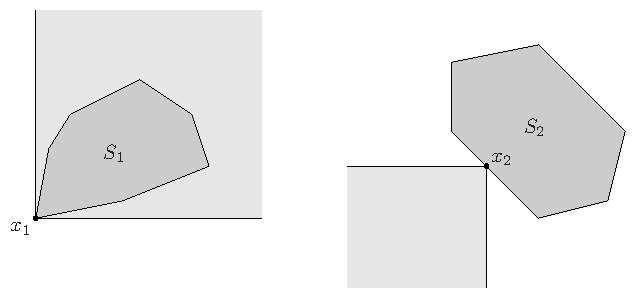
\includegraphics[width=.82\textwidth]{figures/ch02-figure-17.pdf}
\caption*{图2.17\quad 左：集合 $S_1$ 关于 $\R^2$ 中逐分量不等式有最小元 $x_1$。$x_1+K$ 以浅色阴影表示；由于 $S_1\subseteq x_1+K$，$x_1$ 是最小元。右：$x_2$ 是 $S_2$ 的极小点。$x_2-K$ 以浅色阴影表示；因为 $x_2-K$ 与 $S_2$ 仅在 $x_2$ 处相交，所以 $x_2$ 为极小点。}
\end{figure}

\section{分离超平面与支撑超平面}
\subsection{分离超平面定理}
本节介绍一个在后面十分重要的思想：用超平面或仿射函数分离不相交的凸集。基本结果是\emph{分离超平面定理}：设 $C$ 和 $D$ 为非空、不相交的凸集，即 $C\cap D=\varnothing$。那么存在 $a\ne0$ 和 $b$，使对所有 $x\in C$ 有 $a^{\T}x\le b$，对所有 $x\in D$ 有 $a^{\T}x\ge b$。换言之，仿射函数 $a^{\T}x-b$ 在 $C$ 上非正，在 $D$ 上非负。超平面 $\{x\mid a^{\T}x=b\}$ 称为集合 $C$ 和 $D$ 的\emph{分离超平面}，或称它\emph{分离}了 $C$ 和 $D$，见图2.19。

\subsubsection*{分离超平面定理的证明}
这里考虑一个特殊情形，一般情形的证明留作习题2.22。假设 $C$ 与 $D$ 的欧几里得距离
\[
 \dist(C,D)=\inf\{\norm{u-v}_2\mid u\in C,\ v\in D\}
\]
为正，而且存在 $c\in C$、$d\in D$ 取到这个最小距离，即 $\norm{c-d}_2=\dist(C,D)$。例如，$C$、$D$ 都闭且其中一个有界时，这些条件成立。

% Source PDF page 61 (printed p. 47)
\begin{figure}[htbp]\centering
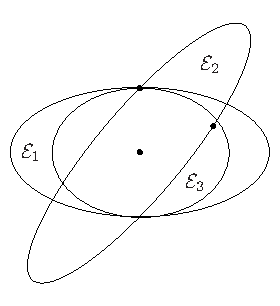
\includegraphics[width=.67\textwidth]{figures/ch02-figure-18.pdf}
\caption*{图2.18\quad $\R^2$ 中三个以原点（下方实点）为中心、包含上方各实点的椭球。$\mathcal E_1$ 不是极小的，因为存在更小、且仍包含这些点的椭球，例如 $\mathcal E_3$；$\mathcal E_3$ 也因同样理由不是极小的。$\mathcal E_2$ 是极小的，因为不存在另一个以原点为中心、包含这些点且包含于 $\mathcal E_2$ 中的椭球。}
\end{figure}
\begin{figure}[htbp]\centering
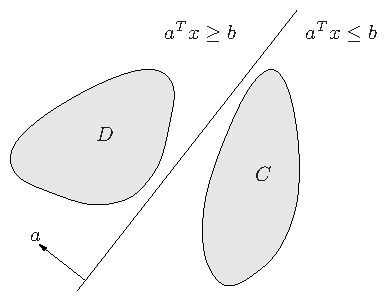
\includegraphics[width=.67\textwidth]{figures/ch02-figure-19.pdf}
\caption*{图2.19\quad 超平面 $\{x\mid a^{\T}x=b\}$ 分离了不相交的凸集 $C$ 和 $D$。仿射函数 $a^{\T}x-b$ 在 $C$ 上非正，在 $D$ 上非负。}
\end{figure}

% Source PDF page 62 (printed p. 48)
\begin{figure}[htbp]\centering
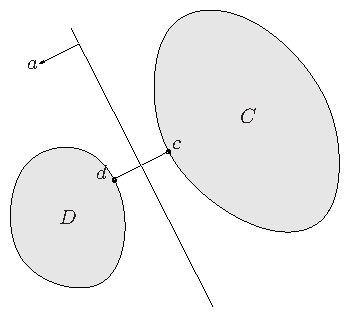
\includegraphics[width=.65\textwidth]{figures/ch02-figure-20.pdf}
\caption*{图2.20\quad 两个凸集之间分离超平面的构造。$c\in C$、$d\in D$ 是两个集合中彼此距离最近的一对点。分离超平面垂直平分 $c$ 与 $d$ 之间的线段。}
\end{figure}
定义
\[
 a=d-c,\qquad b=\frac{\norm d_2^2-\norm c_2^2}{2}.
\]
我们将证明，仿射函数
\[
 f(x)=a^{\T}x-b=(d-c)^{\T}\bigl(x-(1/2)(d+c)\bigr)
\]
在 $C$ 上非正，在 $D$ 上非负，即超平面 $\{x\mid a^{\T}x=b\}$ 分离 $C$ 与 $D$。如图2.20所示，这个超平面与线段 $cd$ 垂直，且经过其中点。

先证明 $f$ 在 $D$ 上非负。$f$ 在 $C$ 上非正的证明类似，也可以交换 $C$ 与 $D$ 并考虑 $-f$ 得到。假设存在 $u\in D$，使
\begin{equation}
 f(u)=(d-c)^{\T}\bigl(u-(1/2)(d+c)\bigr)<0.\tag{2.16}
\end{equation}
可将 $f(u)$ 写成
\[
\begin{aligned}
 f(u)&=(d-c)^{\T}\bigl(u-d+(1/2)(d-c)\bigr)\\
 &=(d-c)^{\T}(u-d)+(1/2)\norm{d-c}_2^2.
\end{aligned}
\]
因此，（2.16）蕴含 $(d-c)^{\T}(u-d)<0$。又有
\[
 \left.\frac{\mathrm d}{\mathrm dt}\norm{d+t(u-d)-c}_2^2\right|_{t=0}
 =2(d-c)^{\T}(u-d)<0,
\]
所以存在足够小的 $t>0$，且 $t\le1$，使
\[
 \norm{d+t(u-d)-c}_2<\norm{d-c}_2.
\]

% Source PDF page 63 (printed p. 49)
也就是说，$d+t(u-d)$ 比 $d$ 更接近 $c$。由于 $D$ 凸，且包含 $d$ 和 $u$，有 $d+t(u-d)\in D$。但这不可能，因为已经假设 $d$ 是 $D$ 中距 $C$ 最近的点。

\begin{origexample}{2.19}
\textbf{仿射集与凸集的分离。}设 $C$ 凸，$D$ 仿射，即 $D=\{Fu+g\mid u\in\R^m\}$，其中 $F\in\R^{n\times m}$。若 $C$、$D$ 不相交，则由分离超平面定理，存在 $a\ne0$ 和 $b$，使 $C$ 上有 $a^{\T}x\le b$，$D$ 上有 $a^{\T}x\ge b$。

条件 $a^{\T}x\ge b$ 对所有 $x\in D$ 成立，意味着 $a^{\T}Fu\ge b-a^{\T}g$ 对所有 $u\in\R^m$ 成立。但线性函数在整个 $\R^m$ 上有下界，只有当其恒为零时才可能。因此 $a^{\T}F=0$，进而 $b\le a^{\T}g$。

综上，存在 $a\ne0$，使 $F^{\T}a=0$，且对所有 $x\in C$ 有 $a^{\T}x\le a^{\T}g$。
\end{origexample}

\subsubsection*{严格分离}
上面构造的分离超平面满足更强的条件：对所有 $x\in C$，$a^{\T}x<b$；对所有 $x\in D$，$a^{\T}x>b$。这称为集合 $C$ 和 $D$ 的\emph{严格分离}。简单例子表明，一般情况下，不相交的凸集未必能被一个超平面严格分离，即使两者都闭也如此，见习题2.23。但在许多特殊情形下，可以证明严格分离成立。

\begin{origexample}{2.20}
\textbf{一点与闭凸集的严格分离。}设 $C$ 为闭凸集，$x_0\notin C$，则存在一个超平面将 $x_0$ 与 $C$ 严格分离。

为证明这一点，注意到存在 $\epsilon>0$，使 $C$ 与 $B(x_0,\epsilon)$ 不相交。由分离超平面定理，存在 $a\ne0$ 和 $b$，使 $x\in C$ 时 $a^{\T}x\le b$，$x\in B(x_0,\epsilon)$ 时 $a^{\T}x\ge b$。

利用 $B(x_0,\epsilon)=\{x_0+u\mid\norm u_2\le\epsilon\}$，第二个条件可写为
\[
 a^{\T}(x_0+u)\ge b,\qquad\text{对所有 }\norm u_2\le\epsilon.
\]
使左边最小的 $u$ 是 $u=-\epsilon a/\norm a_2$，代入得
\[
 a^{\T}x_0-\epsilon\norm a_2\ge b.
\]
因此，仿射函数
\[
 f(x)=a^{\T}x-b-\epsilon\norm a_2/2
\]
在 $C$ 上为负，在 $x_0$ 处为正。

这还立即证明了前面提到的事实：闭凸集是所有包含它的半空间的交。事实上，设 $C$ 闭且凸，$S$ 为所有包含 $C$ 的半空间之交。显然，$x\in C$ 蕴含 $x\in S$。反过来，假设存在 $x\in S$、$x\notin C$。由严格分离的结果，存在超平面严格分离 $x$ 与 $C$，即存在一个包含 $C$ 但不包含 $x$ 的半空间。换言之，$x\notin S$。
\end{origexample}

% Source PDF page 64 (printed p. 50)
\subsubsection*{逆分离超平面定理}
分离超平面定理的逆命题，即存在分离超平面就蕴含 $C$ 和 $D$ 不相交，并不成立，除非在凸性之外，对 $C$ 或 $D$ 施加额外条件。一个简单反例是 $C=D=\{0\}\subseteq\R$，超平面 $x=0$ 分离了 $C$ 和 $D$。

通过增加关于 $C$ 和 $D$ 的条件，可以得到各种逆分离定理。一个非常简单的例子是：设 $C$、$D$ 凸，且 $C$ 开；若存在仿射函数 $f$，使它在 $C$ 上非正、在 $D$ 上非负，则 $C$ 和 $D$ 不相交。为说明这一点，先注意到 $f$ 在 $C$ 上必为负；若 $f$ 在 $C$ 中某点为零，就会在该点附近取正值，从而矛盾。由于 $f$ 在 $C$ 上为负、在 $D$ 上非负，$C$ 与 $D$ 必不相交。将这个逆命题与分离超平面定理结合，得到：任意两个凸集 $C$ 和 $D$，若至少一个开，则它们不相交，当且仅当存在分离超平面。

\begin{origexample}{2.21}
\textbf{严格线性不等式的择一定理。}我们推导严格线性不等式组
\begin{equation}
 Ax\prec b\tag{2.17}
\end{equation}
有解的充要条件。这组不等式不可行，当且仅当两个凸集
\[
 C=\{b-Ax\mid x\in\R^n\},\qquad
 D=\R_{++}^m=\{y\in\R^m\mid y\succ0\}
\]
不相交。$D$ 开，$C$ 仿射，因此由上述结果，$C$ 与 $D$ 不相交，当且仅当存在分离超平面，即存在非零 $\lambda\in\R^m$ 和 $\mu\in\R$，使在 $C$ 上有 $\lambda^{\T}y\le\mu$，在 $D$ 上有 $\lambda^{\T}y\ge\mu$。

这两个条件都可以简化。第一个意味着对所有 $x$ 有 $\lambda^{\T}(b-Ax)\le\mu$。与例2.19一样，这推出 $A^{\T}\lambda=0$、$\lambda^{\T}b\le\mu$。第二个意味着对所有 $y\succ0$ 有 $\lambda^{\T}y\ge\mu$，推出 $\mu\le0$、$\lambda\succeq0$、$\lambda\ne0$。

综合可得，严格不等式组（2.17）不可行，当且仅当存在 $\lambda\in\R^m$ 满足
\begin{equation}
 \lambda\ne0,\qquad\lambda\succeq0,\qquad
 A^{\T}\lambda=0,\qquad\lambda^{\T}b\le0.\tag{2.18}
\end{equation}
这也是关于变量 $\lambda\in\R^m$ 的线性不等式和线性等式组。我们称（2.17）和（2.18）构成一对\emph{择一系统}：对任意数据 $A$、$b$，其中恰有一个有解。
\end{origexample}

\subsection{支撑超平面}
设 $C\subseteq\R^n$，$x_0$ 为其边界 $\operatorname{bd}C$ 上的一点，即
\[
 x_0\in\operatorname{bd}C=\cl C\setminus\operatorname{int}C.
\]
如果 $a\ne0$ 满足对所有 $x\in C$ 都有 $a^{\T}x\le a^{\T}x_0$，则超平面 $\{x\mid a^{\T}x=a^{\T}x_0\}$ 称为 $C$ 在点 $x_0$ 处的\emph{支撑超平面}。

% Source PDF page 65 (printed p. 51)
这等价于说，点 $x_0$ 与集合 $C$ 被超平面 $\{x\mid a^{\T}x=a^{\T}x_0\}$ 分离。几何上，该超平面在 $x_0$ 处与 $C$ 相切，且半空间 $\{x\mid a^{\T}x\le a^{\T}x_0\}$ 包含 $C$，见图2.21。
\begin{figure}[htbp]\centering
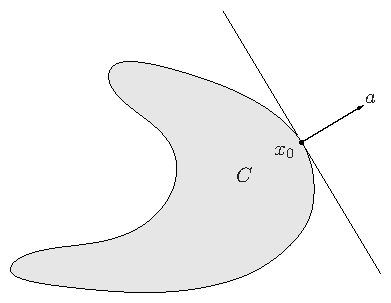
\includegraphics[width=.65\textwidth]{figures/ch02-figure-21.pdf}
\caption*{图2.21\quad 超平面 $\{x\mid a^{\T}x=a^{\T}x_0\}$ 在 $x_0$ 处支撑 $C$。}
\end{figure}
一个称为\emph{支撑超平面定理}的基本结果指出：对任意非空凸集 $C$ 和任意 $x_0\in\operatorname{bd}C$，都存在 $C$ 在 $x_0$ 处的支撑超平面。由分离超平面定理容易证明这一结果，分两种情形。若 $C$ 的内部非空，则对 $\{x_0\}$ 和 $\operatorname{int}C$ 应用分离超平面定理即可。若 $C$ 的内部为空，则 $C$ 必位于维数小于 $n$ 的仿射集中，任何包含这一仿射集的超平面都包含 $C$ 和 $x_0$，因此是一个平凡的支撑超平面。

支撑超平面定理也有部分逆命题：如果集合闭、内部非空，且每个边界点处都有支撑超平面，那么该集合凸，见习题2.27。

\section{对偶锥与广义不等式}
\subsection{对偶锥}
设 $K$ 是一个锥，集合
\begin{equation}
 K^*=\{y\mid x^{\T}y\ge0,\ \text{对所有 }x\in K\}\tag{2.19}
\end{equation}
称为 $K$ 的\emph{对偶锥}。顾名思义，$K^*$ 是一个锥，而且它总是凸的，即使原来的锥 $K$ 非凸也如此，见习题2.31。

几何上，$y\in K^*$ 当且仅当 $-y$ 是一个在原点支撑 $K$ 的超平面的法向量，见图2.22。

\begin{origexample}{2.22}
\textbf{子空间。}子空间 $V\subseteq\R^n$ 也是一个锥，其对偶锥为正交补
\[
 V^{\perp}=\{y\mid v^{\T}y=0,\ \text{对所有 }v\in V\}.
\]
\end{origexample}

% Source PDF page 66 (printed p. 52)
\begin{figure}[htbp]\centering
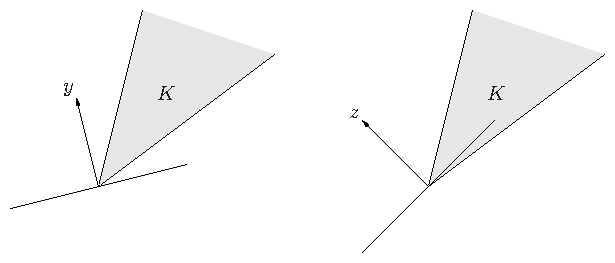
\includegraphics[width=.80\textwidth]{figures/ch02-figure-22.pdf}
\caption*{图2.22\quad 左：内法向量为 $y$ 的半空间包含锥 $K$，因此 $y\in K^*$。右：内法向量为 $z$ 的半空间不包含 $K$，因此 $z\notin K^*$。}
\end{figure}

\begin{origexample}{2.23}
\textbf{非负正交锥。}锥 $\R_+^n$ 的对偶是自身：
\[
 x^{\T}y\ge0\ \text{对所有 }x\succeq0
 \quad\Longleftrightarrow\quad y\succeq0.
\]
这样的锥称为\emph{自对偶锥}。
\end{origexample}

\begin{origexample}{2.24}
\textbf{半正定锥。}在对称 $n\times n$ 矩阵空间 $\mathbf S^n$ 上，采用标准内积
$\tr(XY)=\sum_{i,j=1}^nX_{ij}Y_{ij}$，见第A.1.1节。半正定锥 $\mathbf S_+^n$ 自对偶，即对 $X,Y\in\mathbf S^n$，有
\[
 \tr(XY)\ge0\ \text{对所有 }X\succeq0
 \quad\Longleftrightarrow\quad Y\succeq0.
\]
下面证明这一点。

若 $Y\notin\mathbf S_+^n$，则存在 $q\in\R^n$，使
\[
 q^{\T}Yq=\tr(qq^{\T}Y)<0.
\]
于是，半正定矩阵 $X=qq^{\T}$ 满足 $\tr(XY)<0$，从而 $Y\notin(\mathbf S_+^n)^*$。

再设 $X,Y\in\mathbf S_+^n$。由特征值分解可写 $X=\sum_{i=1}^n\lambda_iq_iq_i^{\T}$，其中各特征值 $\lambda_i\ge0$，$i=1,\ldots,n$。因此
\[
 \tr(YX)=\tr\left(Y\sum_{i=1}^n\lambda_iq_iq_i^{\T}\right)
 =\sum_{i=1}^n\lambda_iq_i^{\T}Yq_i\ge0,
\]
故 $Y\in(\mathbf S_+^n)^*$。
\end{origexample}

\begin{origexample}{2.25}
\textbf{范数锥的对偶。}设 $\norm{\cdot}$ 是 $\R^n$ 上的范数。相关锥
$K=\{(x,t)\in\R^{n+1}\mid\norm x\le t\}$ 的对偶，是由对偶范数定义的锥，即
\[
 K^*=\{(u,v)\in\R^{n+1}\mid\norm u_*\le v\},
\]
其中对偶范数为 $\norm u_*=\sup\{u^{\T}x\mid\norm x\le1\}$，见（A.1.6）。

% Source PDF page 67 (printed p. 53)
要证明这一结果，需说明
\begin{equation}
 \bigl[x^{\T}u+tv\ge0\ \text{只要 }\norm x\le t\bigr]
 \quad\Longleftrightarrow\quad\norm u_*\le v.\tag{2.20}
\end{equation}
先证明关于 $(u,v)$ 的右侧条件蕴含左侧条件。设 $\norm u_*\le v$，且对某个 $t>0$ 有 $\norm x\le t$。如果 $t=0$，则 $x$ 必为零，显然 $u^{\T}x+vt\ge0$。由对偶范数定义及 $\norm{-x/t}\le1$，有
\[
 u^{\T}(-x/t)\le\norm u_*\le v,
\]
因而 $u^{\T}x+vt\ge0$。

再证明（2.20）左侧蕴含右侧。假设 $\norm u_*>v$，即右侧不成立。由对偶范数定义，存在 $x$，满足 $\norm x\le1$ 且 $x^{\T}u>v$。取 $t=1$，有
\[
 u^{\T}(-x)+v<0,
\]
与（2.20）左侧条件矛盾。
\end{origexample}

对偶锥满足以下性质：
\begin{itemize}
\item $K^*$ 闭且凸。
\item $K_1\subseteq K_2$ 蕴含 $K_2^*\subseteq K_1^*$。
\item 如果 $K$ 的内部非空，则 $K^*$ 尖。
\item 如果 $K$ 的闭包尖，则 $K^*$ 内部非空。
\item $K^{**}$ 是 $K$ 的凸包的闭包。因此，若 $K$ 凸且闭，则 $K^{**}=K$。
\end{itemize}
见习题2.31。这些性质表明，如果 $K$ 是正常锥，则对偶锥 $K^*$ 也正常，而且 $K^{**}=K$。

\subsection{对偶广义不等式}
现在，设凸锥 $K$ 正常，从而诱导广义不等式 $\preceq_K$。对偶锥 $K^*$ 也正常，因此同样诱导一个广义不等式。将 $\preceq_{K^*}$ 称为 $\preceq_K$ 的\emph{对偶广义不等式}。两者的重要联系包括：
\begin{itemize}
\item $x\preceq_K y$，当且仅当对所有 $\lambda\succeq_{K^*}0$，有 $\lambda^{\T}x\le\lambda^{\T}y$。
\item $x\prec_K y$，当且仅当对所有 $\lambda\succeq_{K^*}0$、$\lambda\ne0$，有 $\lambda^{\T}x<\lambda^{\T}y$。
\end{itemize}
由于 $K=K^{**}$，$\preceq_{K^*}$ 的对偶广义不等式是 $\preceq_K$，所以上述性质在交换广义不等式与其对偶后仍成立。例如，$\lambda\preceq_{K^*}\mu$，当且仅当对所有 $x\succeq_K0$，有 $\lambda^{\T}x\le\mu^{\T}x$。

% Source PDF page 68 (printed p. 54)
\begin{origexample}{2.26}
\textbf{严格线性广义不等式的择一定理。}设 $K\subseteq\R^m$ 为正常锥，考虑严格广义不等式
\begin{equation}
 Ax\prec_K b,\tag{2.21}
\end{equation}
其中 $x\in\R^n$。

我们推导这一不等式的择一定理。假设它不可行，即仿射集 $\{b-Ax\mid x\in\R^n\}$ 与开凸集 $\operatorname{int}K$ 不相交。那么存在分离超平面，即非零 $\lambda\in\R^m$ 和 $\mu\in\R$，使对所有 $x$ 有 $\lambda^{\T}(b-Ax)\le\mu$，对所有 $y\in\operatorname{int}K$ 有 $\lambda^{\T}y\ge\mu$。第一个条件推出 $A^{\T}\lambda=0$、$\lambda^{\T}b\le\mu$。第二个条件推出对所有 $y\in K$ 有 $\lambda^{\T}y\ge\mu$，这只有在 $\lambda\in K^*$ 且 $\mu\le0$ 时才可能成立。

综合可得，如果（2.21）不可行，则存在 $\lambda$ 满足
\begin{equation}
 \lambda\ne0,\qquad\lambda\succeq_{K^*}0,\qquad
 A^{\T}\lambda=0,\qquad\lambda^{\T}b\le0.\tag{2.22}
\end{equation}
再证明逆命题：若（2.22）成立，则不等式组（2.21）必不可行。假设两者都成立。由于 $\lambda\ne0$、$\lambda\succeq_{K^*}0$、$b-Ax\succ_K0$，有 $\lambda^{\T}(b-Ax)>0$。但由 $A^{\T}\lambda=0$ 又得 $\lambda^{\T}(b-Ax)=\lambda^{\T}b\le0$，矛盾。

因此，不等式组（2.21）与（2.22）互为择一系统：对任意 $A,b$，恰有一个可行。这推广了 $K=\R_+^m$ 时的择一系统（2.17）、（2.18）。
\end{origexample}

\subsection{通过对偶不等式刻画最小元与极小元}
可用对偶广义不等式刻画集合 $S\subseteq\R^m$ 关于正常锥 $K$ 所诱导广义不等式的最小元与极小元，这里的 $S$ 可以非凸。

\subsubsection*{最小元的对偶刻画}
先考虑最小元的刻画：$x$ 是 $S$ 关于 $\preceq_K$ 的最小元，当且仅当对所有 $\lambda\succ_{K^*}0$，$x$ 都是在 $z\in S$ 上最小化 $\lambda^{\T}z$ 的唯一解。几何上，这意味着对任意 $\lambda\succ_{K^*}0$，超平面
\[
 \{z\mid\lambda^{\T}(z-x)=0\}
\]
都是 $S$ 在 $x$ 处的严格支撑超平面。“严格支撑”指超平面与 $S$ 仅在 $x$ 处相交。这里不要求 $S$ 凸，见图2.23。

为证明这一结果，假设 $x$ 是 $S$ 的最小元，即对所有 $z\in S$ 都有 $x\preceq_K z$，并取 $\lambda\succ_{K^*}0$。对 $z\in S$、$z\ne x$，由于 $x$ 是最小元，有 $z-x\succeq_K0$。结合 $\lambda\succ_{K^*}0$ 和 $z-x\ne0$，得 $\lambda^{\T}(z-x)>0$。$z$ 是 $S$ 中任意不同于 $x$ 的点，因此 $x$ 是 $\lambda^{\T}z$ 在 $S$ 上的唯一最小点。

反过来，假设对所有 $\lambda\succ_{K^*}0$，$x$ 都是 $\lambda^{\T}z$ 在 $S$ 上的唯一最小点，但 $x$ 不是 $S$ 的最小元。

% Source PDF page 69 (printed p. 55)
\begin{figure}[htbp]\centering
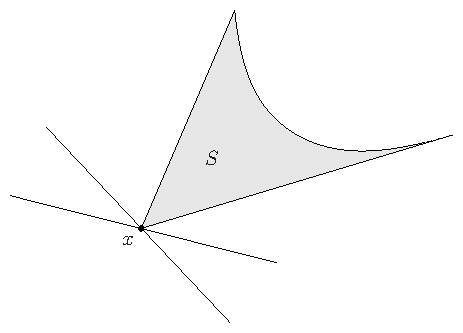
\includegraphics[width=.60\textwidth]{figures/ch02-figure-23.pdf}
\caption*{图2.23\quad 最小元的对偶刻画。$x$ 是集合 $S$ 关于 $\R_+^2$ 的最小元，等价地，对每个 $\lambda\succ0$，超平面 $\{z\mid\lambda^{\T}(z-x)=0\}$ 都在 $x$ 处严格支撑 $S$，即 $S$ 全部位于其一侧，且仅在 $x$ 处接触超平面。}
\end{figure}
那么存在 $z\in S$，使 $z\not\succeq_K x$。由于 $z-x\not\succeq_K0$，存在 $\widetilde\lambda\succeq_{K^*}0$，使 $\widetilde\lambda^{\T}(z-x)<0$。因此，在 $\widetilde\lambda$ 邻域内可取 $\lambda\succ_{K^*}0$，使 $\lambda^{\T}(z-x)<0$，这与 $x$ 是 $\lambda^{\T}z$ 在 $S$ 上的唯一最小点相矛盾。

\subsubsection*{极小元的对偶刻画}
接下来考虑极小元的类似刻画。这里的必要条件与充分条件之间存在差距。如果 $\lambda\succ_{K^*}0$，且 $x$ 在 $z\in S$ 上最小化 $\lambda^{\T}z$，则 $x$ 是极小元，见图2.24。

为证明这一点，设 $\lambda\succ_{K^*}0$，且 $x$ 在 $S$ 上最小化 $\lambda^{\T}z$，但 $x$ 不是极小元。也就是说，存在 $z\in S$、$z\ne x$ 且 $z\preceq_K x$。于是 $\lambda^{\T}(x-z)>0$，与 $x$ 是 $S$ 上的最小点这一假设矛盾。

逆命题一般不成立：某点 $x$ 可以是 $S$ 的极小元，却对任意 $\lambda$ 都不是 $\lambda^{\T}z$ 在 $S$ 上的最小点，见图2.25。这个图提示凸性在逆命题中起着重要作用，事实也确实如此。若 $S$ 凸，则对每个极小元 $x$，都存在非零 $\lambda\succeq_{K^*}0$，使 $x$ 在 $S$ 上最小化 $\lambda^{\T}z$。

为证明这一点，设 $x$ 极小，即 $((x-K)\setminus\{x\})\cap S=\varnothing$。对凸集 $(x-K)\setminus\{x\}$ 和 $S$ 应用分离超平面定理，得存在 $\lambda\ne0$ 和 $\mu$，使对所有 $y\in K$ 有 $\lambda^{\T}(x-y)\le\mu$，对所有 $z\in S$ 有 $\lambda^{\T}z\ge\mu$。第一个不等式推出 $\lambda\succeq_{K^*}0$。因为 $x\in S$ 且 $x\in x-K$，有 $\lambda^{\T}x=\mu$，第二个不等式因此表明，$\mu$ 是 $\lambda^{\T}z$ 在 $S$ 上的最小值。所以，$x$ 是 $\lambda^{\T}z$ 在 $S$ 上的最小点，其中 $\lambda\ne0$、$\lambda\succeq_{K^*}0$。

这个逆定理中的条件不能加强为 $\lambda\succ_{K^*}0$。例子表明，一个点 $x$ 可以是凸集 $S$ 的极小点，却对任意 $\lambda\succ_{K^*}0$ 都不是 $\lambda^{\T}z$ 在 $S$ 上的最小点。

% Source PDF page 70 (printed p. 56)
\begin{figure}[htbp]\centering
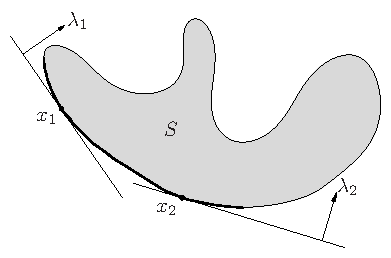
\includegraphics[width=.66\textwidth]{figures/ch02-figure-24.pdf}
\caption*{图2.24\quad 集合 $S\subseteq\R^2$。关于 $\R_+^2$ 的极小点集，是左下边界上以深色表示的部分。$\lambda_1^{\T}z$ 在 $S$ 上的最小点为 $x_1$，由于 $\lambda_1\succ0$，它是极小点。$\lambda_2^{\T}z$ 在 $S$ 上的最小点为 $x_2$，由于 $\lambda_2\succ0$，它也是 $S$ 的极小点。}
\end{figure}
\begin{figure}[htbp]\centering
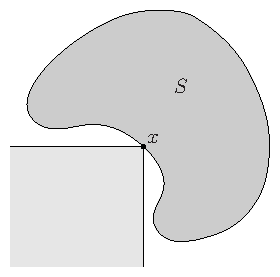
\includegraphics[width=.60\textwidth]{figures/ch02-figure-25.pdf}
\caption*{图2.25\quad 点 $x$ 是 $S\subseteq\R^2$ 关于 $\R_+^2$ 的极小元，但不存在使 $x$ 在 $z\in S$ 上最小化 $\lambda^{\T}z$ 的 $\lambda$。}
\end{figure}

% Source PDF page 71 (printed p. 57)
\begin{figure}[htbp]\centering
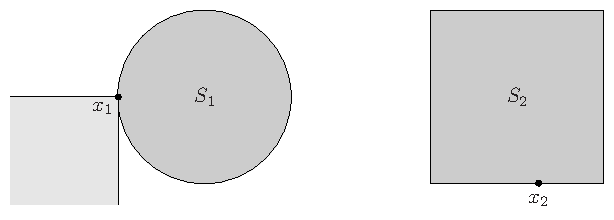
\includegraphics[width=.82\textwidth]{figures/ch02-figure-26.pdf}
\caption*{图2.26\quad 左：点 $x_1\in S_1$ 极小，但对任意 $\lambda\succ0$，都不是 $\lambda^{\T}z$ 在 $S_1$ 上的最小点。不过，当 $\lambda=(1,0)$ 时，它确实在 $z\in S_1$ 上最小化 $\lambda^{\T}z$。右：点 $x_2\in S_2$ 不极小，但当 $\lambda=(0,1)\succeq0$ 时，它是在 $z\in S_2$ 上最小化 $\lambda^{\T}z$ 的点。}
\end{figure}
前述不能加强条件的情形见图2.26左图。同时，也不能说：当 $\lambda\succeq_{K^*}0$ 时，$\lambda^{\T}z$ 在 $S$ 上的每个最小点都是极小元，见图2.26右图。

\begin{origexample}{2.27}
\textbf{Pareto最优生产前沿。}考虑制造某种产品，需要使用 $n$ 种资源，例如劳动力、电力、天然气和水。产品有多种制造或生产方法。对每种生产方法，关联资源向量 $x\in\R^n$，$x_i$ 表示该方法生产产品所消耗的第 $i$ 种资源的数量。假设 $x_i\ge0$，即生产方法消耗资源；同时资源具有价值，因此任何一种资源都希望用得更少。

\emph{生产集} $P\subseteq\R^n$ 定义为所有对应某种生产方法的资源向量 $x$ 构成的集合。

若某种生产方法的资源向量是 $P$ 关于逐分量不等式的极小元，就称该生产方法为\emph{Pareto最优}或\emph{有效}的。$P$ 的极小元集称为\emph{有效生产前沿}。

Pareto最优性有一个简单解释。若资源向量为 $x$ 的方法与资源向量为 $y$ 的方法相比，满足所有 $i$ 都有 $x_i\le y_i$，并且至少一个 $i$ 有 $x_i<y_i$，就称前者\emph{优于}后者。换言之，一种方法在每项资源的使用量上都不超过另一种，并至少有一项严格更少，就更好。这对应 $x\preceq y$、$x\ne y$。因此可以说：没有更好的生产方法时，该生产方法就是Pareto最优或有效的。

选择任意满足 $\lambda\succ0$ 的 $\lambda$，在生产向量集 $P$ 上最小化
\[
 \lambda^{\T}x=\lambda_1x_1+\cdots+\lambda_nx_n,
\]
便能找到Pareto最优生产方法，即极小资源向量。

向量 $\lambda$ 有简单的解释：$\lambda_i$ 是第 $i$ 种资源的价格。在 $P$ 上最小化 $\lambda^{\T}x$，就是寻找给定资源价格 $\lambda_i$ 下总成本最低的生产方法。只要价格均为正，得到的生产方法就保证有效。

图2.27说明了这些概念。
\end{origexample}

% Source PDF page 72 (printed p. 58)
\begin{figure}[htbp]\centering
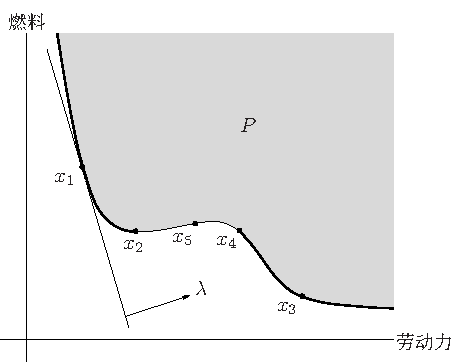
\includegraphics[width=.70\textwidth]{figures/ch02-figure-27.pdf}
\caption*{图2.27\quad 生产某种产品所需的资源为劳动力与燃料，生产集 $P$ 以阴影表示。两条深色曲线是有效生产前沿。点 $x_1$、$x_2$、$x_3$ 有效；点 $x_4$ 和 $x_5$ 无效，特别地，$x_2$ 对应的方法燃料用量不更多，劳动力用量更少。$x_1$ 还是正价格向量 $\lambda$ 下成本最低的生产方法。$x_2$ 有效，但不能通过对任何价格向量 $\lambda\succeq0$ 最小化总成本 $\lambda^{\T}x$ 找到。}
\end{figure}

% Source PDF page 73 (printed p. 59)
\section*{文献说明}
\addcontentsline{toc}{section}{文献说明}
通常认为，Minkowski 首先系统研究了凸集，并引入支撑超平面、支撑超平面定理、Minkowski距离函数（习题3.34）、凸集的极点等许多基本概念。

一些著名的早期综述包括 Bonnesen 和 Fenchel [BF48]、Eggleston [Egg58]、Klee [Kle63] 和 Valentine [Val64]。较新、专门讨论凸集几何的著作有 Lay [Lay82] 和 Webster [Web94]。Klee [Kle71]、Fenchel [Fen83]、Tikhomorov [Tik90] 和 Berger [Ber90] 对凸性的历史及其在数学各领域中的应用，给出了十分易读的概述。

线性不等式和多面体集，与线性规划密切相关，已经得到广泛研究；相关文献见第4章末。线性不等式与线性规划历史上的一些里程碑著作包括 Motzkin [Mot33]、von Neumann 和 Morgenstern [vNM53]、Kantorovich [Kan60]、Koopmans [Koo51] 和 Dantzig [Dan63]。Dantzig [Dan63，第2章] 综述了截至1963年前后的线性不等式发展史。

广义不等式在20世纪60年代被引入非线性优化，参见 Luenberger [Lue69，第8.2节] 和 Isii [Isi64]，此后广泛应用于锥规划，见第4章参考文献。Bellman 和 Fan [BF63] 是研究相对于半正定锥的广义线性不等式组的一篇早期论文。

分离超平面定理的证明及扩展，可参阅 Rockafellar [Roc70，第三部分] 以及 Hiriart-Urruty 和 Lemar\'echal [HUL93，第1卷，第III4节]。Dantzig [Dan63，第21页] 将“择一定理”这一术语归于 von Neumann 和 Morgenstern [vNM53，第138页]。更多择一定理文献见第5章。

例2.27中的术语，包括Pareto最优性、有效生产和 $\lambda$ 的价格解释，见 Luenberger [Lue95] 的详细讨论。

凸几何在经典矩理论中占有重要地位，参见 Krein 和 Nudelman [KN77]、Karlin 和 Studden [KS66]。一个著名例子是非负多项式锥与幂矩锥之间的对偶关系，见习题2.37。

% Source PDF page 74 (printed p. 60)
\section*{习题}
\addcontentsline{toc}{section}{习题}
\subsection*{凸性的定义}
\paragraph{2.1}
设 $C\subseteq\R^n$ 为凸集，$x_1,\ldots,x_k\in C$，$\theta_1,\ldots,\theta_k\in\R$ 满足 $\theta_i\ge0$、$\theta_1+\cdots+\theta_k=1$。证明 $\theta_1x_1+\cdots+\theta_kx_k\in C$。凸性的定义只要求 $k=2$ 时成立，这里需对任意 $k$ 证明。\emph{提示：}对 $k$ 使用归纳法。

\paragraph{2.2}
证明：一个集合凸，当且仅当它与任意直线的交凸。证明：一个集合仿射，当且仅当它与任意直线的交仿射。

\paragraph{2.3}
\textbf{中点凸性。}如果只要 $a,b\in C$，两者的平均值或中点 $(a+b)/2$ 就在 $C$ 中，则称 $C$ 为\emph{中点凸集}。显然，凸集一定中点凸。可以证明，在较弱条件下，中点凸性蕴含凸性。证明一个简单情形：如果 $C$ 闭且中点凸，则 $C$ 凸。

\paragraph{2.4}
证明：集合 $S$ 的凸包是所有包含 $S$ 的凸集的交。同样的方法还可证明，$S$ 的锥包、仿射包或线性包，分别为所有包含 $S$ 的锥集、仿射集或子空间的交。

\subsection*{例子}
\paragraph{2.5}
两个平行超平面 $\{x\in\R^n\mid a^{\T}x=b_1\}$ 与 $\{x\in\R^n\mid a^{\T}x=b_2\}$ 之间的距离是多少？

\paragraph{2.6}
一个半空间何时包含另一个半空间？给出下式成立的条件：
\[
 \{x\mid a^{\T}x\le b\}\subseteq
 \{x\mid\widetilde a^{\T}x\le\widetilde b\},
\]
其中 $a\ne0$、$\widetilde a\ne0$。再找出两个半空间相等的条件。

\paragraph{2.7}
\textbf{半空间的Voronoi描述。}设 $a,b$ 是 $\R^n$ 中不同的点。证明：所有到 $a$ 的欧几里得距离不超过到 $b$ 的距离的点组成的集合，即
$\{x\mid\norm{x-a}_2\le\norm{x-b}_2\}$，是半空间。将它明确写成 $c^{\T}x\le d$ 的形式，并画图说明。

\paragraph{2.8}
下列集合 $S$ 中，哪些是多面体？若可能，将 $S$ 写成 $S=\{x\mid Ax\preceq b,\ Fx=g\}$ 的形式。
\begin{enumerate}[label=(\alph*)]
\item $S=\{y_1a_1+y_2a_2\mid-1\le y_1\le1,\ -1\le y_2\le1\}$，其中 $a_1,a_2\in\R^n$。
\item $S=\{x\in\R^n\mid x\succeq0,\ \one^{\T}x=1,\ \sum_{i=1}^nx_ia_i=b_1,\ \sum_{i=1}^nx_ia_i^2=b_2\}$，其中 $a_1,\ldots,a_n\in\R$、$b_1,b_2\in\R$。
\item $S=\{x\in\R^n\mid x\succeq0,\ x^{\T}y\le1,\ \text{对所有满足 }\norm y_2=1\text{ 的 }y\}$。
\item $S=\{x\in\R^n\mid x\succeq0,\ x^{\T}y\le1,\ \text{对所有满足 }\sum_{i=1}^n\abs{y_i}=1\text{ 的 }y\}$。
\end{enumerate}

\paragraph{2.9}
\textbf{Voronoi集与多面体分解。}设 $x_0,\ldots,x_K\in\R^n$ 两两不同。考虑到 $x_0$ 的欧几里得距离不超过到其他各 $x_i$ 的距离的点集，即
\[
 V=\{x\in\R^n\mid\norm{x-x_0}_2\le\norm{x-x_i}_2,\ i=1,\ldots,K\}.
\]
$V$ 称为相对于 $x_1,\ldots,x_K$ 的 $x_0$ 的\emph{Voronoi区域}。
\begin{enumerate}[label=(\alph*)]
\item 证明 $V$ 是多面体，并写成 $V=\{x\mid Ax\preceq b\}$。
\item 反过来，给定内部非空的多面体 $P$，说明如何找到 $x_0,\ldots,x_K$，使该多面体正是相对于 $x_1,\ldots,x_K$ 的 $x_0$ 的Voronoi区域。
\item 还可考虑集合
\[
 V_k=\{x\in\R^n\mid\norm{x-x_k}_2\le\norm{x-x_i}_2,\ i\ne k\}.
\]
$V_k$ 由 $\R^n$ 中那些在集合 $\{x_0,\ldots,x_K\}$ 中以 $x_k$ 为最近点的点组成。

% Source PDF page 75 (printed p. 61)
集合 $V_0,\ldots,V_K$ 给出 $\R^n$ 的一个\emph{多面体分解}。更准确地说，$V_k$ 都是内部非空的多面体，$\bigcup_{k=0}^KV_k=\R^n$，且当 $i\ne j$ 时，$\operatorname{int}V_i\cap\operatorname{int}V_j=\varnothing$，也就是说，$V_i$ 与 $V_j$ 至多在边界处相交。

设 $P_1,\ldots,P_m$ 为内部非空的多面体，满足 $\bigcup_{i=1}^mP_i=\R^n$，且对 $i\ne j$ 有 $\operatorname{int}P_i\cap\operatorname{int}P_j=\varnothing$。这样的 $\R^n$ 多面体分解，能否描述为某组适当点生成的Voronoi区域？
\end{enumerate}

\paragraph{2.10}
\textbf{二次不等式的解集。}设 $C\subseteq\R^n$ 为二次不等式的解集，
\[
 C=\{x\in\R^n\mid x^{\T}Ax+b^{\T}x+c\le0\},
\]
其中 $A\in\mathbf S^n$、$b\in\R^n$、$c\in\R$。
\begin{enumerate}[label=(\alph*)]
\item 证明：若 $A\succeq0$，则 $C$ 凸。
\item 证明：若存在 $\lambda\in\R$ 使 $A+\lambda gg^{\T}\succeq0$，则 $C$ 与超平面 $g^{\T}x+h=0$ 的交凸，其中 $g\ne0$。
\end{enumerate}
这些结论的逆命题是否成立？

\paragraph{2.11}
\textbf{双曲集。}证明双曲集 $\{x\in\R_+^2\mid x_1x_2\ge1\}$ 凸。进而证明 $\{x\in\R_+^n\mid\prod_{i=1}^nx_i\ge1\}$ 凸。\emph{提示：}若 $a,b\ge0$、$0\le\theta\le1$，则 $a^\theta b^{1-\theta}\le\theta a+(1-\theta)b$，见第3.1.9节。

\paragraph{2.12}
下列集合中哪些是凸集？
\begin{enumerate}[label=(\alph*)]
\item 带状区域，即形如 $\{x\in\R^n\mid\alpha\le a^{\T}x\le\beta\}$ 的集合。
\item 矩形，即 $\{x\in\R^n\mid\alpha_i\le x_i\le\beta_i,\ i=1,\ldots,n\}$。当 $n>2$ 时，矩形有时称为超矩形。
\item 楔形区域，即 $\{x\in\R^n\mid a_1^{\T}x\le b_1,\ a_2^{\T}x\le b_2\}$。
\item 到给定点的距离不超过到给定集合的距离的点集，即
\[
 \{x\mid\norm{x-x_0}_2\le\norm{x-y}_2,\ \text{对所有 }y\in S\},
\]
其中 $S\subseteq\R^n$。
\item 到某个集合的距离不超过到另一个集合的距离的点集，即
\[
 \{x\mid\dist(x,S)\le\dist(x,T)\},
\]
其中 $S,T\subseteq\R^n$，且
\[
 \dist(x,S)=\inf\{\norm{x-z}_2\mid z\in S\}.
\]
\item [HUL93，第1卷，第93页] 集合 $\{x\mid x+S_2\subseteq S_1\}$，其中 $S_1,S_2\subseteq\R^n$，且 $S_1$ 凸。
\item 到 $a$ 的距离不超过到 $b$ 的距离的固定比例 $\theta$ 的点集，即 $\{x\mid\norm{x-a}_2\le\theta\norm{x-b}_2\}$。可假设 $a\ne b$ 且 $0\le\theta\le1$。
\end{enumerate}

\paragraph{2.13}
\textbf{外积的锥包。}考虑秩为 $k$ 的外积所成的集合 $\{XX^{\T}\mid X\in\R^{n\times k},\ \rank X=k\}$。用简单形式描述其锥包。

\paragraph{2.14}
\textbf{扩张集与收缩集。}设 $S\subseteq\R^n$，$\norm{\cdot}$ 是 $\R^n$ 上的范数。
\begin{enumerate}[label=(\alph*)]
\item 对 $a\ge0$，定义 $S_a=\{x\mid\dist(x,S)\le a\}$，其中 $\dist(x,S)=\inf_{y\in S}\norm{x-y}$。称 $S_a$ 为 $S$ 扩张或延伸 $a$ 后的集合。证明：若 $S$ 凸，则 $S_a$ 凸。
\item 对 $a\ge0$，定义 $S_{-a}=\{x\mid B(x,a)\subseteq S\}$，其中 $B(x,a)$ 是范数 $\norm{\cdot}$ 下以 $x$ 为中心、半径为 $a$ 的球。称 $S_{-a}$ 为 $S$ 收缩或限制 $a$ 后的集合，因为其中各点到 $\R^n\setminus S$ 的距离至少为 $a$。证明：若 $S$ 凸，则 $S_{-a}$ 凸。
\end{enumerate}

% Source PDF page 76 (printed p. 62)
\paragraph{2.15}
\textbf{一些概率分布集合。}设 $x$ 为实值随机变量，$\Prob(x=a_i)=p_i$，$i=1,\ldots,n$，其中 $a_1<a_2<\cdots<a_n$。当然，$p\in\R^n$ 位于标准概率单纯形 $P=\{p\mid\one^{\T}p=1,\ p\succeq0\}$ 中。下列哪些条件关于 $p$ 是凸的？也就是说，哪些条件使满足条件的 $p\in P$ 构成凸集？
\begin{enumerate}[label=(\alph*)]
\item $\alpha\le\E f(x)\le\beta$，其中 $\E f(x)=\sum_{i=1}^np_if(a_i)$ 为 $f(x)$ 的期望，给定函数为 $f:\R\to\R$。
\item $\Prob(x>\alpha)\le\beta$。
\item $\E\abs{x^3}\le\alpha\E\abs x$。
\item $\E x^2\le\alpha$。
\item $\E x^2\ge\alpha$。
\item $\operatorname{var}(x)\le\alpha$，其中 $\operatorname{var}(x)=\E(x-\E x)^2$ 为 $x$ 的方差。
\item $\operatorname{var}(x)\ge\alpha$。
\item $\operatorname{quartile}(x)\ge\alpha$，其中 $\operatorname{quartile}(x)=\inf\{\beta\mid\Prob(x\le\beta)\ge0.25\}$。
\item $\operatorname{quartile}(x)\le\alpha$。
\end{enumerate}

\subsection*{保持凸性的运算}
\paragraph{2.16}
证明：若 $S_1$ 和 $S_2$ 是 $\R^{m+n}$ 中的凸集，则其部分和
\[
 S=\{(x,y_1+y_2)\mid x\in\R^m,\ y_1,y_2\in\R^n,
 \ (x,y_1)\in S_1,\ (x,y_2)\in S_2\}
\]
也凸。

\paragraph{2.17}
\textbf{多面体集在透视函数下的像。}研究超平面、半空间及多面体在透视函数 $P(x,t)=x/t$、$\dom P=\R^n\times\R_{++}$ 下的像。对下列各集合 $C$，给出
\[
 P(C)=\{v/t\mid(v,t)\in C,\ t>0\}
\]
的简单描述。
\begin{enumerate}[label=(\alph*)]
\item 多面体 $C=\conv\{(v_1,t_1),\ldots,(v_K,t_K)\}$，其中 $v_i\in\R^n$、$t_i>0$。
\item 超平面 $C=\{(v,t)\mid f^{\T}v+gt=h\}$，$f$ 与 $g$ 不同时为零。
\item 半空间 $C=\{(v,t)\mid f^{\T}v+gt\le h\}$，$f$ 与 $g$ 不同时为零。
\item 多面体 $C=\{(v,t)\mid Fv+gt\preceq h\}$。
\end{enumerate}

\paragraph{2.18}
\textbf{可逆的线性分式函数。}设线性分式函数 $f:\R^n\to\R^n$ 为
\[
 f(x)=(Ax+b)/(c^{\T}x+d),\qquad\dom f=\{x\mid c^{\T}x+d>0\}.
\]
假设矩阵
\[
 Q=\begin{bmatrix}A&b\\c^{\T}&d\end{bmatrix}
\]
非奇异。证明 $f$ 可逆，且 $f^{-1}$ 是线性分式映射。用 $A,b,c,d$ 给出 $f^{-1}$ 及其定义域的显式表达式。\emph{提示：}用 $Q$ 表示 $f^{-1}$ 可能更容易。

\paragraph{2.19}
\textbf{线性分式函数与凸集。}设线性分式函数 $f:\R^m\to\R^n$ 为
\[
 f(x)=(Ax+b)/(c^{\T}x+d),\qquad\dom f=\{x\mid c^{\T}x+d>0\}.
\]
本题研究凸集 $C$ 在 $f$ 下的逆像，即
\[
 f^{-1}(C)=\{x\in\dom f\mid f(x)\in C\}.
\]
对下列各集合 $C\subseteq\R^n$，给出 $f^{-1}(C)$ 的简单描述。
\begin{enumerate}[label=(\alph*)]
\item 半空间 $C=\{y\mid g^{\T}y\le h\}$，其中 $g\ne0$。
\item 多面体 $C=\{y\mid Gy\preceq h\}$。
\item 椭球 $\{y\mid y^{\T}P^{-1}y\le1\}$，其中 $P\in\mathbf S_{++}^n$。
\item 线性矩阵不等式的解集 $C=\{y\mid y_1A_1+\cdots+y_nA_n\preceq B\}$，其中 $A_1,\ldots,A_n,B\in\mathbf S^p$。
\end{enumerate}

% Source PDF page 77 (printed p. 63)
\subsection*{分离定理与支撑超平面}
\paragraph{2.20}
\textbf{线性方程的严格正解。}设 $A\in\R^{m\times n}$、$b\in\R^m$，且 $b\in\mathcal R(A)$。证明：存在 $x$ 满足
\[
 x\succ0,\qquad Ax=b,
\]
当且仅当不存在 $\lambda$ 满足
\[
 A^{\T}\lambda\succeq0,\qquad A^{\T}\lambda\ne0,\qquad b^{\T}\lambda\le0.
\]
\emph{提示：}先证明以下线性代数事实：对所有满足 $Ax=b$ 的 $x$ 都有 $c^{\T}x=d$，当且仅当存在向量 $\lambda$，使 $c=A^{\T}\lambda$、$d=b^{\T}\lambda$。

\paragraph{2.21}
\textbf{分离超平面的集合。}设 $C$、$D$ 是 $\R^n$ 中不相交的子集。考虑所有 $(a,b)\in\R^{n+1}$ 构成的集合，其中对所有 $x\in C$ 有 $a^{\T}x\le b$，对所有 $x\in D$ 有 $a^{\T}x\ge b$。证明它是凸锥；如果没有超平面分离 $C$ 和 $D$，该集合为单点集 $\{0\}$。

\paragraph{2.22}
补全第2.5.1节的分离超平面定理证明：证明任意两个不相交的凸集 $C$、$D$ 之间都存在分离超平面。可以使用第2.5.1节已经证明的结果，即当两个集合中有一对点的距离等于两集合距离时，存在分离超平面。

\emph{提示：}若 $C$ 和 $D$ 是不相交的凸集，则集合 $\{x-y\mid x\in C,\ y\in D\}$ 凸且不包含原点。

\paragraph{2.23}
举出两个闭凸集的例子，它们不相交，但不能被严格分离。

\paragraph{2.24}
\textbf{支撑超平面。}
\begin{enumerate}[label=(\alph*)]
\item 将闭凸集 $\{x\in\R_+^2\mid x_1x_2\ge1\}$ 表示为若干半空间的交。
\item 设 $C=\{x\in\R^n\mid\norm x_\infty\le1\}$ 为 $\R^n$ 中 $\ell_\infty$ 范数单位球，$\widehat x$ 为 $C$ 的边界点。明确找出 $C$ 在 $\widehat x$ 处的支撑超平面。
\end{enumerate}

\paragraph{2.25}
\textbf{多面体内外逼近。}设 $C\subseteq\R^n$ 为闭凸集，$x_1,\ldots,x_K$ 位于 $C$ 的边界。对每个 $i$，假设 $a_i^{\T}(x-x_i)=0$ 定义 $C$ 在 $x_i$ 处的支撑超平面，即 $C\subseteq\{x\mid a_i^{\T}(x-x_i)\le0\}$。考虑两个多面体
\[
\begin{aligned}
 P_{\mathrm{inner}}&=\conv\{x_1,\ldots,x_K\},\\
 P_{\mathrm{outer}}&=\{x\mid a_i^{\T}(x-x_i)\le0,\ i=1,\ldots,K\}.
\end{aligned}
\]
证明 $P_{\mathrm{inner}}\subseteq C\subseteq P_{\mathrm{outer}}$，并画图说明。

\paragraph{2.26}
\textbf{支撑函数。}集合 $C\subseteq\R^n$ 的支撑函数定义为
\[
 S_C(y)=\sup\{y^{\T}x\mid x\in C\}.
\]
允许 $S_C(y)$ 取值 $+\infty$。设 $C$、$D$ 是 $\R^n$ 中的闭凸集。证明：$C=D$ 当且仅当两者的支撑函数相等。

\paragraph{2.27}
\textbf{逆支撑超平面定理。}设集合 $C$ 闭、内部非空，且在每个边界点处都有支撑超平面。证明 $C$ 凸。

\subsection*{凸锥与广义不等式}
\paragraph{2.28}
\textbf{$n=1,2,3$ 时的半正定锥。}对 $n=1,2,3$，用矩阵元素和普通不等式给出半正定锥 $\mathbf S_+^n$ 的显式描述。分别使用下列记号表示 $\mathbf S^n$ 中的一般元素：
\[
 x_1,\qquad
 \begin{bmatrix}x_1&x_2\\x_2&x_3\end{bmatrix},\qquad
 \begin{bmatrix}x_1&x_2&x_3\\x_2&x_4&x_5\\x_3&x_5&x_6\end{bmatrix}.
\]

% Source PDF page 78 (printed p. 64)
\paragraph{2.29}
\textbf{$\R^2$ 中的锥。}设 $K\subseteq\R^2$ 为闭凸锥。
\begin{enumerate}[label=(\alph*)]
\item 用元素的极坐标 $x=r(\cos\phi,\sin\phi)$、$r\ge0$，给出 $K$ 的简单描述。
\item 给出 $K^*$ 的简单描述，并画图说明 $K$ 与 $K^*$ 的关系。
\item $K$ 在什么条件下是尖的？
\item $K$ 在什么条件下是正常的，从而定义广义不等式？画图说明当 $K$ 正常时，$x\preceq_K y$ 的含义。
\end{enumerate}

\paragraph{2.30}
\textbf{广义不等式的性质。}证明第2.4.1节列出的非严格与严格广义不等式的各项性质。

\paragraph{2.31}
\textbf{对偶锥的性质。}设 $K^*$ 为凸锥 $K$ 的对偶锥，定义见（2.19）。证明下列结论。
\begin{enumerate}[label=(\alph*)]
\item $K^*$ 确实为凸锥。
\item $K_1\subseteq K_2$ 蕴含 $K_2^*\subseteq K_1^*$。
\item $K^*$ 闭。
\item $K^*$ 的内部为 $\operatorname{int}K^*=\{y\mid y^{\T}x>0,\ \text{对所有 }x\in\cl K\}$。
\item 如果 $K$ 内部非空，则 $K^*$ 尖。
\item $K^{**}$ 是 $K$ 的闭包。因此，若 $K$ 闭，则 $K^{**}=K$。
\item 如果 $K$ 的闭包尖，则 $K^*$ 内部非空。
\end{enumerate}

\paragraph{2.32}
求 $\{Ax\mid x\succeq0\}$ 的对偶锥，其中 $A\in\R^{m\times n}$。

\paragraph{2.33}
\textbf{单调非负锥。}定义单调非负锥
\[
 K_{m+}=\{x\in\R^n\mid x_1\ge x_2\ge\cdots\ge x_n\ge0\},
\]
即所有分量按非递增次序排列的非负向量构成的集合。
\begin{enumerate}[label=(\alph*)]
\item 证明 $K_{m+}$ 为正常锥。
\item 求对偶锥 $K_{m+}^*$。\emph{提示：}使用恒等式
\[
\begin{aligned}
 \sum_{i=1}^n x_iy_i
 &=(x_1-x_2)y_1+(x_2-x_3)(y_1+y_2)\\
 &\quad +(x_3-x_4)(y_1+y_2+y_3)+\cdots\\
 &\quad +(x_{n-1}-x_n)(y_1+\cdots+y_{n-1})
       +x_n(y_1+\cdots+y_n).
\end{aligned}
\]
\end{enumerate}

\paragraph{2.34}
\textbf{字典序锥与字典序。}字典序锥定义为
\[
 K_{\mathrm{lex}}=\{0\}\cup
 \{x\in\R^n\mid x_1=\cdots=x_k=0,\ x_{k+1}>0,
 \ \text{对某个 }k,\ 0\le k<n\},
\]
即所有第一个非零分量为正的向量，以及零向量。
\begin{enumerate}[label=(\alph*)]
\item 验证 $K_{\mathrm{lex}}$ 是锥，但不是正常锥。
\item 定义 $\R^n$ 上的\emph{字典序}：$x\le_{\mathrm{lex}}y$ 当且仅当 $y-x\in K_{\mathrm{lex}}$。因为 $K_{\mathrm{lex}}$ 不是正常锥，字典序不属于广义不等式。证明字典序为全序：对任意 $x,y\in\R^n$，$x\le_{\mathrm{lex}}y$ 或 $y\le_{\mathrm{lex}}x$ 总有一个成立。因此，可以按字典序锥对任意一组向量排序，得到字典中熟悉的排序方式。
\item 求 $K_{\mathrm{lex}}^*$。
\end{enumerate}

\paragraph{2.35}
\textbf{共正矩阵。}若矩阵 $X\in\mathbf S^n$ 对所有 $z\succeq0$ 满足 $z^{\T}Xz\ge0$，则称 $X$ 为\emph{共正矩阵}。验证共正矩阵集合为正常锥，并求其对偶锥。

% Source PDF page 79 (printed p. 65)
\paragraph{2.36}
\textbf{欧几里得距离矩阵。}设 $x_1,\ldots,x_n\in\R^k$。由 $D_{ij}=\norm{x_i-x_j}_2^2$ 定义的矩阵 $D\in\mathbf S^n$ 称为\emph{欧几里得距离矩阵}。它满足一些显然的性质，例如 $D_{ij}=D_{ji}$、$D_{ii}=0$、$D_{ij}\ge0$；由三角不等式还有 $D_{ik}^{1/2}\le D_{ij}^{1/2}+D_{jk}^{1/2}$。

现在问：矩阵 $D\in\mathbf S^n$ 什么时候是某个 $\R^k$ 中某些点的欧几里得距离矩阵？一个著名结果回答了这一问题：$D\in\mathbf S^n$ 是欧几里得距离矩阵，当且仅当 $D_{ii}=0$，且对所有满足 $\one^{\T}x=0$ 的 $x$，有 $x^{\T}Dx\le0$，见第8.3.3节。

证明欧几里得距离矩阵的集合为凸锥。

\paragraph{2.37}
\textbf{非负多项式与Hankel线性矩阵不等式。}设 $K_{\mathrm{pol}}$ 为 $\R$ 上非负的 $2k$ 次多项式的系数集：
\[
 K_{\mathrm{pol}}=\{x\in\R^{2k+1}\mid
 x_1+x_2t+x_3t^2+\cdots+x_{2k+1}t^{2k}\ge0,
 \ \text{对所有 }t\in\R\}.
\]
\begin{enumerate}[label=(\alph*)]
\item 证明 $K_{\mathrm{pol}}$ 是正常锥。
\item 一个基本结果指出：$2k$ 次多项式在 $\R$ 上非负，当且仅当它可以写成两个次数不超过 $k$ 的多项式的平方和。换言之，$x\in K_{\mathrm{pol}}$，当且仅当多项式
\[
 p(t)=x_1+x_2t+x_3t^2+\cdots+x_{2k+1}t^{2k}
\]
可写成
\[
 p(t)=r(t)^2+s(t)^2,
\]
其中 $r$、$s$ 是 $k$ 次多项式。

利用该结果证明
\[
 K_{\mathrm{pol}}=\left\{x\in\R^{2k+1}\ \middle|\
 x_i=\sum_{m+n=i+1}Y_{mn},\ \text{对某个 }Y\in\mathbf S_+^{k+1}\right\}.
\]
也就是说，$p(t)=x_1+x_2t+x_3t^2+\cdots+x_{2k+1}t^{2k}$ 非负，当且仅当存在 $Y\in\mathbf S_+^{k+1}$，使
\[
\begin{aligned}
 x_1&=Y_{11},\\
 x_2&=Y_{12}+Y_{21},\\
 x_3&=Y_{13}+Y_{22}+Y_{31},\\
 &\ \vdots\\
 x_{2k+1}&=Y_{k+1,k+1}.
\end{aligned}
\]
\item 证明 $K_{\mathrm{pol}}^*=K_{\mathrm{han}}$，其中
\[
 K_{\mathrm{han}}=\{z\in\R^{2k+1}\mid H(z)\succeq0\},
\]
且
\[
 H(z)=\begin{bmatrix}
 z_1&z_2&z_3&\cdots&z_k&z_{k+1}\\
 z_2&z_3&z_4&\cdots&z_{k+1}&z_{k+2}\\
 z_3&z_4&z_5&\cdots&z_{k+2}&z_{k+4}\\
 \vdots&\vdots&\vdots&\ddots&\vdots&\vdots\\
 z_k&z_{k+1}&z_{k+2}&\cdots&z_{2k-1}&z_{2k}\\
 z_{k+1}&z_{k+2}&z_{k+3}&\cdots&z_{2k}&z_{2k+1}
 \end{bmatrix}.
\]
这是以 $z_1,\ldots,z_{2k+1}$ 为系数的Hankel矩阵。

% Source PDF page 80 (printed p. 66)
\item 设 $K_{\mathrm{mom}}$ 为所有形如 $(1,t,t^2,\ldots,t^{2k})$、$t\in\R$ 的向量的锥包。证明：$y\in K_{\mathrm{mom}}$，当且仅当 $y_1\ge0$，且对某个随机变量 $u$，有
\[
 y=y_1(1,\E u,\E u^2,\ldots,\E u^{2k}).
\]
换言之，$K_{\mathrm{mom}}$ 的元素是 $\R$ 上所有可能分布的矩向量的非负倍数。证明 $K_{\mathrm{pol}}=K_{\mathrm{mom}}^*$。
\item 结合(c)、(d)的结果，推出 $K_{\mathrm{han}}=\cl K_{\mathrm{mom}}$。

作为说明 $K_{\mathrm{mom}}$ 与 $K_{\mathrm{han}}$ 关系的一个例子，取 $k=2$、$z=(1,0,0,0,1)$。证明 $z\in K_{\mathrm{han}}$、$z\notin K_{\mathrm{mom}}$，并给出一个收敛到 $z$ 的 $K_{\mathrm{mom}}$ 中点的显式序列。
\end{enumerate}

\paragraph{2.38}
[Roc70，第15、61页]\quad\textbf{由集合构造凸锥。}
\begin{enumerate}[label=(\alph*)]
\item 集合 $C$ 的\emph{障碍锥}定义为使 $y^{\T}x$ 在 $x\in C$ 上有上界的所有向量 $y$ 构成的集合。换言之，非零向量 $y$ 属于障碍锥，当且仅当它是某个包含 $C$ 的半空间 $\{x\mid y^{\T}x\le\alpha\}$ 的法向量。验证障碍锥为凸锥，不对 $C$ 作任何假设。
\item 集合 $C$ 的\emph{衰退锥}，也称\emph{渐近锥}，定义为所有满足下列条件的向量 $y$ 的集合：对每个 $x\in C$ 和所有 $t\ge0$，均有 $x-ty\in C$。证明凸集的衰退锥是凸锥。证明：如果 $C$ 非空、闭且凸，则 $C$ 的衰退锥是其障碍锥的对偶。
\item 集合 $C$ 在边界点 $x_0$ 处的\emph{法锥}，是所有满足 $y^{\T}(x-x_0)\le0$（对所有 $x\in C$）的向量 $y$ 构成的集合，也就是在 $x_0$ 处定义 $C$ 的支撑超平面的向量集。证明法锥为凸锥，不对 $C$ 作任何假设。简单描述多面体 $\{x\mid Ax\preceq b\}$ 在其边界某点处的法锥。
\end{enumerate}

\paragraph{2.39}
\textbf{锥的分离。}设 $K$、$\widetilde K$ 为两个凸锥，其内部非空且不相交。证明存在非零 $y$，使 $y\in K^*$、$-y\in\widetilde K^*$。


% Source PDF page 81 (printed p. 67)
\chapter{凸函数}
\section{基本性质与例子}
\subsection{定义}
若函数 $f:\R^n\to\R$ 的定义域 $\dom f$ 是凸集，并且对所有 $x,y\in\dom f$ 以及 $0\leq\theta\leq1$，都有
\begin{equation}
 f(\theta x+(1-\theta)y)\leq\theta f(x)+(1-\theta)f(y),\tag{3.1}
\end{equation}
则称 $f$ 为凸函数。

从几何上说，这个不等式意味着，连接 $(x,f(x))$ 与 $(y,f(y))$ 的线段，也就是从 $x$ 到 $y$ 的弦，位于 $f$ 的图像上方（图3.1）。如果只要 $x\ne y$ 且 $0<\theta<1$，式(3.1)中的不等号就严格成立，则称 $f$ 为严格凸函数。若 $-f$ 凸，则称 $f$ 凹；若 $-f$ 严格凸，则称 $f$ 严格凹。

对于仿射函数，式(3.1)总取等号，因此所有仿射函数（从而也包括所有线性函数）都既凸又凹。反过来，既凸又凹的函数必为仿射函数。

一个函数是凸函数，当且仅当把它限制在任意与其定义域相交的直线上时，所得函数都凸。换句话说，$f$ 凸，当且仅当对所有 $x\in\dom f$ 和所有 $v$，函数 $g(t)=f(x+tv)$ 在其定义域 $\{t\mid x+tv\in\dom f\}$ 上凸。
\begin{figure}[htbp]\centering
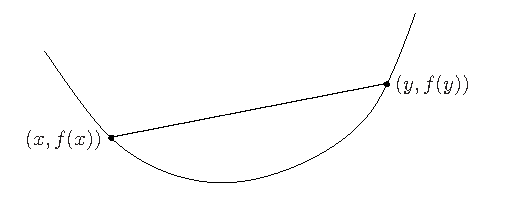
\includegraphics[width=.58\textwidth]{figures/ch03-81.pdf}
\caption*{图3.1 凸函数的图像。连接图像上任意两点的弦（即线段）都位于图像上方。}
\end{figure}
% Source PDF page 82 (printed p. 68)
这一性质很有用，因为它使我们能够通过将函数限制在直线上，检查函数的凸性。

凸函数分析是一个发展完善的领域，本书不作深入讨论。例如，一个简单结论是：凸函数在其定义域的相对内部连续；不连续只能出现在相对边界上。

\subsection{扩展值延拓}
把凸函数在定义域外的值定义为 $\infty$，从而将它延拓到整个 $\R^n$，往往很方便。若 $f$ 凸，定义其扩展值延拓 $\widetilde f:\R^n\to\R\cup\{\infty\}$ 为
\[
 \widetilde f(x)=\begin{cases}f(x),&x\in\dom f,\\ \infty,&x\notin\dom f.\end{cases}
\]
延拓 $\widetilde f$ 在整个 $\R^n$ 上有定义，取值于 $\R\cup\{\infty\}$。原函数的定义域可以从延拓恢复：$\dom f=\{x\mid\widetilde f(x)<\infty\}$。

延拓可以简化记号，因为我们不必显式描述定义域，也不必每次提到 $f(x)$ 时都加上“对所有 $x\in\dom f$”这一限定。例如，基本定义不等式(3.1)用延拓 $\widetilde f$ 可以写为：当 $0<\theta<1$ 时，对任意 $x,y$ 都有
\[
 \widetilde f(\theta x+(1-\theta)y)
 \leq\theta\widetilde f(x)+(1-\theta)\widetilde f(y).
\]
（当 $\theta=0$ 或 $\theta=1$ 时，不等式总成立。）这里当然必须用扩展算术与次序来理解不等式。若 $x,y$ 都属于 $\dom f$，它就与式(3.1)相同；若其中一点在定义域外，则右端为 $\infty$，因此不等式成立。

再看这种记号用法的另一个例子。设 $f_1,f_2$ 是 $\R^n$ 上的两个凸函数。逐点和 $f=f_1+f_2$ 的定义域为 $\dom f=\dom f_1\cap\dom f_2$，且对任意 $x\in\dom f$ 有 $f(x)=f_1(x)+f_2(x)$。用扩展值延拓，我们只需说，对任意 $x$ 都有 $\widetilde f(x)=\widetilde f_1(x)+\widetilde f_2(x)$。在此等式中，$f$ 的定义域自动成为 $\dom f_1\cap\dom f_2$，因为只要 $x\notin\dom f_1$ 或 $x\notin\dom f_2$，就有 $\widetilde f(x)=\infty$。这个例子利用扩展算术自动确定了定义域。

在本书中，只要歧义不会造成问题，就用同一个符号表示凸函数及其延拓。这相当于假定所有凸函数都已隐式延拓，即在定义域外取值 $\infty$。

\begin{origexample}{3.1}
\textbf{凸集的示性函数。}设 $C\subseteq\R^n$ 为凸集，考虑定义域为 $C$、在所有 $x\in C$ 处满足 $I_C(x)=0$ 的凸函数 $I_C$。换句话说，这个函数在 $C$ 上恒为零。它的扩展值延拓为
% Source PDF page 83 (printed p. 69)
\[
 \widetilde I_C(x)=\begin{cases}0,&x\in C,\\ \infty,&x\notin C.\end{cases}
\]
凸函数 $\widetilde I_C$ 称为集合 $C$ 的示性函数。

示性函数 $\widetilde I_C$ 可以带来几种方便的记号处理。例如，在集合 $C$ 上最小化函数 $f$（不妨设它在整个 $\R^n$ 上有定义），等同于在整个 $\R^n$ 上最小化函数 $f+\widetilde I_C$。事实上，按我们的约定，$f+\widetilde I_C$ 就是 $f$ 在 $C$ 上的限制。
\end{origexample}
类似地，可令凹函数在定义域外取值 $-\infty$，得到它的延拓。
\begin{figure}[htbp]\centering
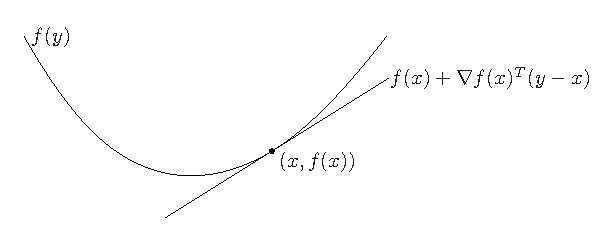
\includegraphics[width=.65\textwidth]{figures/ch03-83.pdf}
\caption*{图3.2 若 $f$ 凸且可微，则对所有 $x,y\in\dom f$ 都有 $f(x)+\nabla f(x)^\T(y-x)\leq f(y)$。}
\end{figure}
\subsection{一阶条件}
假设 $f$ 可微，即它的梯度 $\nabla f$ 在开集 $\dom f$ 中的每一点都存在。那么，$f$ 凸，当且仅当 $\dom f$ 凸，且对所有 $x,y\in\dom f$ 都有
\begin{equation}
 f(y)\geq f(x)+\nabla f(x)^\T(y-x).\tag{3.2}
\end{equation}
图3.2说明了这个不等式。

关于 $y$ 的仿射函数 $f(x)+\nabla f(x)^\T(y-x)$，正是 $f$ 在 $x$ 附近的一阶 Taylor 近似。不等式(3.2)表明：对于凸函数，一阶 Taylor 近似实际上是函数的全局下估计。反过来，如果函数的一阶 Taylor 近似总是全局下估计，则该函数凸。

不等式(3.2)表明，从凸函数的局部信息（即某一点的函数值与导数）能够导出全局信息（即全局下估计）。这也许是凸函数最重要的性质，并解释了凸函数及凸优化问题的一些突出特点。举一个简单例子，由式(3.2)，若 $\nabla f(x)=0$，则对所有 $y\in\dom f$ 都有 $f(y)\geq f(x)$，也就是说，$x$ 是函数 $f$ 的一个全局最小点。
% Source PDF page 84 (printed p. 70)
严格凸性也可以用一阶条件刻画：$f$ 严格凸，当且仅当 $\dom f$ 凸，且对 $x,y\in\dom f$、$x\ne y$ 有
\begin{equation}
 f(y)>f(x)+\nabla f(x)^\T(y-x).\tag{3.3}
\end{equation}
对于凹函数有相应刻画：$f$ 凹，当且仅当 $\dom f$ 凸，并且对所有 $x,y\in\dom f$ 都有
\[f(y)\leq f(x)+\nabla f(x)^\T(y-x).\]

\subsubsection*{凸性一阶条件的证明}
为证明式(3.2)，先考虑 $n=1$ 的情形。我们将证明，可微函数 $f:\R\to\R$ 凸，当且仅当对定义域内所有 $x,y$ 都有
\begin{equation}
 f(y)\geq f(x)+f'(x)(y-x).\tag{3.4}
\end{equation}
先设 $f$ 凸且 $x,y\in\dom f$。由于 $\dom f$ 凸（即为区间），对所有 $0<t\leq1$ 都有 $x+t(y-x)\in\dom f$，再由 $f$ 的凸性得到
\[f(x+t(y-x))\leq(1-t)f(x)+tf(y).\]
两边除以 $t$ 并整理，得到
\[f(y)\geq f(x)+\frac{f(x+t(y-x))-f(x)}{t}.\]
令 $t\to0$，即得式(3.4)。

为证明充分性，假设函数对 $\dom f$（一个区间）中的所有 $x,y$ 都满足式(3.4)。任取 $x\ne y$、$0\leq\theta\leq1$，令 $z=\theta x+(1-\theta)y$。两次应用式(3.4)，得
\[
 f(x)\geq f(z)+f'(z)(x-z),\qquad
 f(y)\geq f(z)+f'(z)(y-z).
\]
第一个不等式乘以 $\theta$，第二个乘以 $1-\theta$，再相加，得到
\[\theta f(x)+(1-\theta)f(y)\geq f(z),\]
这证明了 $f$ 凸。

现在证明一般情形 $f:\R^n\to\R$。设 $x,y\in\R^n$，考虑 $f$ 在经过它们的直线上的限制，即函数 $g(t)=f(ty+(1-t)x)$；其导数为 $g'(t)=\nabla f(ty+(1-t)x)^\T(y-x)$。

先假设 $f$ 凸，则 $g$ 凸。根据上面的论证，有 $g(1)\geq g(0)+g'(0)$，即
\[f(y)\geq f(x)+\nabla f(x)^\T(y-x).\]
再假设这个不等式对任意 $x,y$ 都成立。若 $ty+(1-t)x\in\dom f$ 且 $\widetilde t y+(1-\widetilde t)x\in\dom f$，则
\[
\begin{split}
 f(ty+(1-t)x)\geq{}& f(\widetilde t y+(1-\widetilde t)x)\\
 &+\nabla f(\widetilde t y+(1-\widetilde t)x)^\T(y-x)(t-\widetilde t),
\end{split}
\]
也就是 $g(t)\geq g(\widetilde t)+g'(\widetilde t)(t-\widetilde t)$。前面已经证明，这意味着 $g$ 凸。
% Source PDF page 85 (printed p. 71)
\subsection{二阶条件}
现在假设 $f$ 二次可微，也就是说，它的 Hessian 矩阵或二阶导数 $\nabla^2f$ 在开集 $\dom f$ 的每一点都存在。那么，$f$ 凸，当且仅当 $\dom f$ 凸，且 Hessian 矩阵半正定，即对所有 $x\in\dom f$ 有
\[\nabla^2f(x)\succeq0.\]
对于 $\R$ 上的函数，这简化为 $f''(x)\geq0$（同时 $\dom f$ 凸，即为区间），也就是导数单调不减。几何上，条件 $\nabla^2f(x)\succeq0$ 要求函数图像在 $x$ 处具有正的（向上的）曲率。二阶条件的证明留作习题3.8。

类似地，$f$ 凹，当且仅当 $\dom f$ 凸，且对所有 $x\in\dom f$ 都有 $\nabla^2f(x)\preceq0$。二阶条件也能部分刻画严格凸性：若对所有 $x\in\dom f$ 都有 $\nabla^2f(x)\succ0$，则 $f$ 严格凸。但逆命题不成立；例如，函数 $f:\R\to\R$，$f(x)=x^4$ 严格凸，却在 $x=0$ 处的二阶导数为零。

\begin{origexample}{3.2}
\textbf{二次函数。}考虑定义域为 $\R^n$ 的二次函数 $f:\R^n\to\R$，
\[f(x)=\tfrac12x^\T Px+q^\T x+r,\]
其中 $P\in\mathbb S^n$、$q\in\R^n$、$r\in\R$。由于所有 $x$ 处都有 $\nabla^2f(x)=P$，$f$ 凸当且仅当 $P\succeq0$（凹当且仅当 $P\preceq0$）。

二次函数的严格凸性容易刻画：$f$ 严格凸当且仅当 $P\succ0$（严格凹当且仅当 $P\prec0$）。
\end{origexample}
\paragraph{注3.1}在凸性和凹性的一阶、二阶刻画中，不能省去 $\dom f$ 为凸集这一单独要求。例如，定义域为 $\{x\in\R\mid x\ne0\}$ 的函数 $f(x)=1/x^2$，在所有 $x\in\dom f$ 处都满足 $f''(x)>0$，却不是凸函数。

\subsection{例子}
前面已经提到，所有线性函数和仿射函数都凸（也凹），并描述了凸二次函数与凹二次函数。本节再给出几个凸函数和凹函数的例子。先看 $\R$ 上以 $x$ 为变量的函数。
\begin{itemize}
\item \textbf{指数。}对任意 $a\in\R$，$e^{ax}$ 在 $\R$ 上凸。
\item \textbf{幂。}当 $a\geq1$ 或 $a\leq0$ 时，$x^a$ 在 $\R_{++}$ 上凸；当 $0\leq a\leq1$ 时，它凹。
\item \textbf{绝对值的幂。}当 $p\geq1$ 时，$|x|^p$ 在 $\R$ 上凸。
\item \textbf{对数。}$\log x$ 在 $\R_{++}$ 上凹。
% Source PDF page 86 (printed p. 72)
\item \textbf{负熵。}$x\log x$ 是凸函数，定义域可取 $\R_{++}$，也可取 $\R_+$，后者在 $x=0$ 处定义为零。
\end{itemize}
\begin{figure}[htbp]\centering
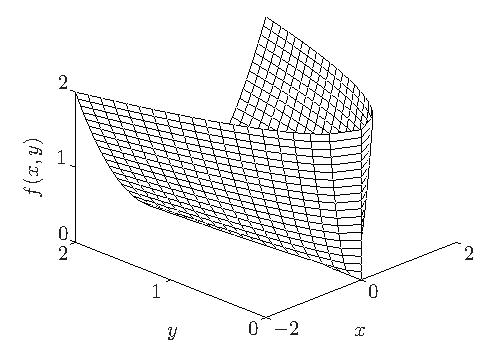
\includegraphics[width=.58\textwidth]{figures/ch03-86.pdf}
\caption*{图3.3 $f(x,y)=x^2/y$ 的图像。}
\end{figure}
这些例子的凸性或凹性，可以通过验证基本不等式(3.1)，或检查二阶导数非负、非正来证明。例如，$f(x)=x\log x$ 有
\[f'(x)=\log x+1,\qquad f''(x)=1/x,\]
所以当 $x>0$ 时 $f''(x)>0$。这说明负熵函数严格凸。

现在给出 $\R^n$ 上几个值得关注的函数例子。
\begin{itemize}
\item \textbf{范数。}$\R^n$ 上的每一个范数都凸。
\item \textbf{最大值函数。}$f(x)=\max\{x_1,\ldots,x_n\}$ 在 $\R^n$ 上凸。
\item \textbf{二次除以线性函数。}$f(x,y)=x^2/y$，定义域为
\[\dom f=\R\times\R_{++}=\{(x,y)\in\R^2\mid y>0\},\]
是凸函数（图3.3）。
\item \textbf{指数和的对数。}$f(x)=\log(e^{x_1}+\cdots+e^{x_n})$ 在 $\R^n$ 上凸。它可以看作最大值函数的可微近似（事实上是解析近似），因为对所有 $x$ 都有
\[
\max\{x_1,\ldots,x_n\}\leq f(x)
 \leq\max\{x_1,\ldots,x_n\}+\log n.
\]
（当 $x$ 的各分量相等时，第二个不等式取等号。）图3.4给出 $n=2$ 时的 $f$。
% Source PDF page 87 (printed p. 73)
\item \textbf{几何平均。}几何平均 $f(x)=(\prod_{i=1}^n x_i)^{1/n}$ 在 $\dom f=\R_{++}^n$ 上凹。
\item \textbf{行列式的对数。}函数 $f(X)=\log\det X$ 在 $\dom f=\mathbb S_{++}^n$ 上凹。
\end{itemize}
\begin{figure}[htbp]\centering
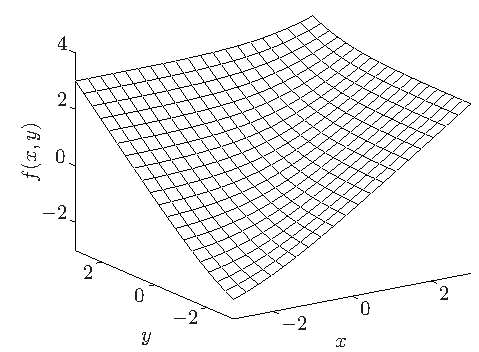
\includegraphics[width=.58\textwidth]{figures/ch03-87.pdf}
\caption*{图3.4 $f(x,y)=\log(e^x+e^y)$ 的图像。}
\end{figure}
这些例子的凸性（或凹性）可以用多种方法验证，例如直接验证不等式(3.1)，检查 Hessian 半正定，或把函数限制在任意一条直线上，再验证所得一元函数的凸性。

\paragraph{范数。}若 $f:\R^n\to\R$ 是范数，且 $0\leq\theta\leq1$，则
\[
 f(\theta x+(1-\theta)y)\leq f(\theta x)+f((1-\theta)y)
 =\theta f(x)+(1-\theta)f(y).
\]
不等式来自三角不等式，等式来自范数的齐次性。

\paragraph{最大值函数。}对 $0\leq\theta\leq1$，函数 $f(x)=\max_i x_i$ 满足
\[
\begin{aligned}
 f(\theta x+(1-\theta)y)&=\max_i(\theta x_i+(1-\theta)y_i)\\
 &\leq\theta\max_i x_i+(1-\theta)\max_i y_i\\
 &=\theta f(x)+(1-\theta)f(y).
\end{aligned}
\]
\paragraph{二次除以线性函数。}为证明 $f(x,y)=x^2/y$ 凸，注意到当 $y>0$ 时，
\[
 \nabla^2f(x,y)=\frac2{y^3}
 \begin{bmatrix}y^2&-xy\\-xy&x^2\end{bmatrix}
 =\frac2{y^3}\begin{bmatrix}y\\-x\end{bmatrix}
 \begin{bmatrix}y\\-x\end{bmatrix}^{\T}\succeq0.
\]
% Source PDF page 88 (printed p. 74)
\paragraph{指数和的对数。}指数和对数函数的 Hessian 为
\[
 \nabla^2 f(x)=\frac1{(\one^\T z)^2}
 \bigl((\one^\T z)\diag(z)-zz^\T\bigr),
\]
其中 $z=(e^{x_1},\ldots,e^{x_n})$。要验证 $\nabla^2f(x)\succeq0$，必须证明对所有 $v$ 有 $v^\T\nabla^2f(x)v\geq0$，即
\[
 v^\T\nabla^2f(x)v=\frac1{(\one^\T z)^2}
 \left(\left(\sum_{i=1}^n z_i\right)\left(\sum_{i=1}^n v_i^2z_i\right)
 -\left(\sum_{i=1}^n v_iz_i\right)^2\right)\geq0.
\]
对分量为 $a_i=v_i\sqrt{z_i}$、$b_i=\sqrt{z_i}$ 的向量应用 Cauchy--Schwarz 不等式 $(a^\T a)(b^\T b)\geq(a^\T b)^2$，便得到所需结论。

\paragraph{几何平均。}类似地，可以证明几何平均 $f(x)=(\prod_{i=1}^n x_i)^{1/n}$ 在 $\dom f=\R_{++}^n$ 上凹。它的 Hessian $\nabla^2f(x)$ 由
\[
 \frac{\partial^2f(x)}{\partial x_k^2}
 =-\frac{(n-1)(\prod_{i=1}^n x_i)^{1/n}}{n^2x_k^2},\qquad
 \frac{\partial^2f(x)}{\partial x_k\partial x_l}
 =\frac{(\prod_{i=1}^n x_i)^{1/n}}{n^2x_kx_l}\quad(k\ne l)
\]
给出，也可以表示为
\[
 \nabla^2 f(x)=-\frac{\prod_{i=1}^n x_i^{1/n}}{n^2}
 \bigl(n\diag(1/x_1^2,\ldots,1/x_n^2)-qq^\T\bigr),
\]
其中 $q_i=1/x_i$。必须证明 $\nabla^2f(x)\preceq0$，即对所有 $v$ 有
\[
 v^\T\nabla^2f(x)v=-\frac{\prod_{i=1}^n x_i^{1/n}}{n^2}
 \left(n\sum_{i=1}^n v_i^2/x_i^2-\left(\sum_{i=1}^n v_i/x_i\right)^2\right)\leq0.
\]
同样，对向量 $a=\one$、$b_i=v_i/x_i$ 应用 Cauchy--Schwarz 不等式 $(a^\T a)(b^\T b)\geq(a^\T b)^2$，就能得到结论。

\paragraph{行列式的对数。}对于 $f(X)=\log\det X$，可以考虑任意直线 $X=Z+tV$（$Z,V\in\mathbb S^n$）来验证凹性。定义 $g(t)=f(Z+tV)$，将 $g$ 限制在满足 $Z+tV\succ0$ 的 $t$ 所构成的区间上。不失一般性，可以假设 $t=0$ 在区间内部，即 $Z\succ0$。有
\[
\begin{aligned}
 g(t)&=\log\det(Z+tV)\\
 &=\log\det\bigl(Z^{1/2}(I+tZ^{-1/2}VZ^{-1/2})Z^{1/2}\bigr)\\
 &=\sum_{i=1}^n\log(1+t\lambda_i)+\log\det Z,
\end{aligned}
\]
其中 $\lambda_1,\ldots,\lambda_n$ 是 $Z^{-1/2}VZ^{-1/2}$ 的特征值。因此
\[
 g'(t)=\sum_{i=1}^n\frac{\lambda_i}{1+t\lambda_i},\qquad
 g''(t)=-\sum_{i=1}^n\frac{\lambda_i^2}{(1+t\lambda_i)^2}.
\]
由于 $g''(t)\leq0$，可知 $f$ 凹。
% Source PDF page 89 (printed p. 75)
\subsection{下水平集}
函数 $f:\R^n\to\R$ 的 $\alpha$-下水平集定义为
\[C_\alpha=\{x\in\dom f\mid f(x)\leq\alpha\}.\]
凸函数的下水平集对任意 $\alpha$ 都是凸集。由凸性的定义可立即证明：若 $x,y\in C_\alpha$，则 $f(x)\leq\alpha$、$f(y)\leq\alpha$，所以对 $0\leq\theta\leq1$ 有 $f(\theta x+(1-\theta)y)\leq\alpha$，从而 $\theta x+(1-\theta)y\in C_\alpha$。

逆命题不成立：一个函数的所有下水平集都可能凸，而函数本身不凸。例如，$f(x)=-e^x$ 在 $\R$ 上不凸（事实上严格凹），但它的所有下水平集都凸。

若 $f$ 凹，则它的 $\alpha$-上水平集 $\{x\in\dom f\mid f(x)\geq\alpha\}$ 是凸集。下水平集性质往往能很好地证明集合的凸性：把集合表示成凸函数的下水平集，或凹函数的上水平集即可。
\begin{origexample}{3.3}
$x\in\R_+^n$ 的几何平均和算术平均分别为
\[G(x)=\left(\prod_{i=1}^n x_i\right)^{1/n},\qquad A(x)=\frac1n\sum_{i=1}^n x_i,\]
其中在 $G$ 的定义中约定 $0^{1/n}=0$。算术—几何平均不等式说明 $G(x)\leq A(x)$。

设 $0\leq\alpha\leq1$，考虑集合
\[\{x\in\R_+^n\mid G(x)\geq\alpha A(x)\},\]
即几何平均至少达到算术平均的 $\alpha$ 倍的向量集合。它是凸集，因为它是凹函数 $G(x)-\alpha A(x)$ 的零上水平集。事实上，这个集合具有正齐次性，所以是凸锥。
\end{origexample}
\subsection{上图}
函数 $f:\R^n\to\R$ 的图像定义为
\[\{(x,f(x))\mid x\in\dom f\},\]
它是 $\R^{n+1}$ 的子集。函数 $f:\R^n\to\R$ 的上图定义为
\[\epi f=\{(x,t)\mid x\in\dom f,\ f(x)\leq t\},\]
也是 $\R^{n+1}$ 的子集。（“epi”表示“在上方”，因此 epigraph 意为“图像上方”。）图3.5说明了这个定义。

凸集与凸函数通过上图联系起来：函数凸，当且仅当它的上图是凸集。函数凹，当且仅当它的下图
\[\operatorname{hypo}f=\{(x,t)\mid t\leq f(x)\}\]
是凸集。
% Source PDF page 90 (printed p. 76)
\begin{figure}[htbp]\centering
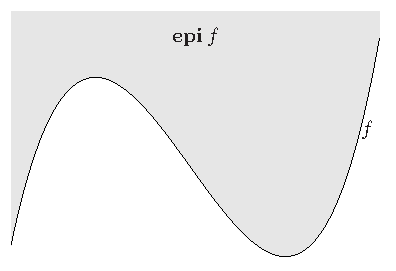
\includegraphics[width=.48\textwidth]{figures/ch03-90.pdf}
\caption*{图3.5 阴影部分是函数 $f$ 的上图。较深的下边界是 $f$ 的图像。}
\end{figure}
\begin{origexample}{3.4}
\textbf{矩阵分式函数。}函数 $f:\R^n\times\mathbb S^n\to\R$，
\[f(x,Y)=x^\T Y^{-1}x,\]
在 $\dom f=\R^n\times\mathbb S_{++}^n$ 上凸。（它推广了定义域为 $\R\times\R_{++}$ 的二次除以线性函数 $f(x,y)=x^2/y$。）

证明 $f$ 凸的一种简便方法是考察其上图：
\[
\begin{aligned}
 \epi f&=\{(x,Y,t)\mid Y\succ0,\ x^\T Y^{-1}x\leq t\}\\
 &=\left\{(x,Y,t)\ \middle|\
 \begin{bmatrix}Y&x\\x^\T&t\end{bmatrix}\succeq0,\ Y\succ0\right\}.
\end{aligned}
\]
这里使用了分块矩阵半正定的 Schur 补条件（见A.5.5节）。最后的条件是关于 $(x,Y,t)$ 的线性矩阵不等式，因此 $\epi f$ 凸。

在特殊情形 $n=1$ 下，矩阵分式函数成为二次除以线性函数 $x^2/y$，对应的 LMI 表示为
\[\begin{bmatrix}y&x\\x&t\end{bmatrix}\succeq0,\qquad y>0\]
（其函数图像见图3.3）。
\end{origexample}
凸函数的许多结论，都可以借助上图并应用凸集结论，从几何上证明或解释。例如，考虑凸性的一阶条件
\[f(y)\geq f(x)+\nabla f(x)^\T(y-x),\]
其中 $f$ 凸、$x,y\in\dom f$。这个基本不等式可以用 $\epi f$ 作几何解释。若 $(y,t)\in\epi f$，则
\[t\geq f(y)\geq f(x)+\nabla f(x)^\T(y-x).\]
% Source PDF page 91 (printed p. 77)
这可以写成
\[
 (y,t)\in\epi f\ \Longrightarrow\
 \begin{bmatrix}\nabla f(x)\\-1\end{bmatrix}^{\T}
 \left(\begin{bmatrix}y\\t\end{bmatrix}
 -\begin{bmatrix}x\\f(x)\end{bmatrix}\right)\leq0.
\]
这意味着，由 $(\nabla f(x),-1)$ 确定的超平面在边界点 $(x,f(x))$ 处支撑 $\epi f$；见图3.6。
\begin{figure}[htbp]\centering
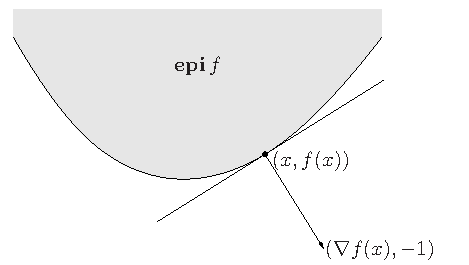
\includegraphics[width=.56\textwidth]{figures/ch03-91.pdf}
\caption*{图3.6 对可微凸函数 $f$，向量 $(\nabla f(x),-1)$ 确定了 $f$ 的上图在 $x$ 处的一个支撑超平面。}
\end{figure}
\subsection{Jensen 不等式及其推广}
基本不等式(3.1)，即
\[f(\theta x+(1-\theta)y)\leq\theta f(x)+(1-\theta)f(y),\]
有时称为 Jensen 不等式。它很容易推广到两个以上点的凸组合：若 $f$ 凸，$x_1,\ldots,x_k\in\dom f$，且 $\theta_1,\ldots,\theta_k\geq0$、$\theta_1+\cdots+\theta_k=1$，则
\[f(\theta_1x_1+\cdots+\theta_kx_k)\leq\theta_1f(x_1)+\cdots+\theta_kf(x_k).\]
如同凸集的情况，不等式还能推广到无穷和、积分与期望。例如，若 $p(x)\geq0$ 对 $S\subseteq\dom f$ 上的 $x$ 成立，且 $\int_S p(x)\,dx=1$，则
\[f\left(\int_S p(x)x\,dx\right)\leq\int_S f(x)p(x)\,dx,\]
只要这些积分存在。最一般的情况可以采用支撑位于 $\dom f$ 内的任意概率测度。若随机变量 $x$ 以概率一属于 $\dom f$，且 $f$ 凸，则
\begin{equation}f(\E x)\leq\E f(x),\tag{3.5}\end{equation}
只要这些期望存在。令随机变量 $x$ 的支撑为 $\{x_1,x_2\}$，且 $\Prob(x=x_1)=\theta$、$\Prob(x=x_2)=1-\theta$，就能从这一一般形式恢复基本不等式(3.1)。
% Source PDF page 92 (printed p. 78)
因此，不等式(3.5)刻画了凸性：若 $f$ 不凸，则存在一个以概率一属于 $\dom f$ 的随机变量 $x$，使 $f(\E x)>\E f(x)$。

现在，上述不等式都称为 Jensen 不等式，尽管 Jensen 研究的只是下面这个很简单的不等式：
\[f\left(\frac{x+y}2\right)\leq\frac{f(x)+f(y)}2.\]
\paragraph{注3.2}式(3.5)可以作如下解释。设 $x\in\dom f\subseteq\R^n$，$z$ 是 $\R^n$ 中任意零均值随机向量。则
\[\E f(x+z)\geq f(x).\]
因此，随机化或抖动（即在自变量上加一个零均值随机向量）不会使凸函数值的平均值降低。

\subsection{不等式}
对合适的凸函数应用 Jensen 不等式，可以导出许多著名不等式。（事实上，凸性与 Jensen 不等式可以作为不等式理论的基础。）举一个简单例子，考虑算术—几何平均不等式：对 $a,b\geq0$ 有
\begin{equation}\sqrt{ab}\leq(a+b)/2.\tag{3.6}\end{equation}
函数 $-\log x$ 凸，取 $\theta=1/2$ 应用 Jensen 不等式，得
\[-\log\frac{a+b}2\leq\frac{-\log a-\log b}2.\]
两边取指数，即得式(3.6)。

再看一个稍复杂的例子，证明 Hölder 不等式：对 $p>1$、$1/p+1/q=1$ 以及 $x,y\in\R^n$，有
\[
 \sum_{i=1}^n x_iy_i\leq
 \left(\sum_{i=1}^n|x_i|^p\right)^{1/p}
 \left(\sum_{i=1}^n|y_i|^q\right)^{1/q}.
\]
由 $-\log x$ 的凸性以及一般 $\theta$ 对应的 Jensen 不等式，得到更一般的算术—几何平均不等式
\[a^\theta b^{1-\theta}\leq\theta a+(1-\theta)b,\]
它对 $a,b\geq0$、$0\leq\theta\leq1$ 成立。取
\[a=\frac{|x_i|^p}{\sum_{j=1}^n|x_j|^p},\qquad
 b=\frac{|y_i|^q}{\sum_{j=1}^n|y_j|^q},\qquad\theta=1/p,\]
应用上述不等式，得
\[
 \left(\frac{|x_i|^p}{\sum_{j=1}^n|x_j|^p}\right)^{1/p}
 \left(\frac{|y_i|^q}{\sum_{j=1}^n|y_j|^q}\right)^{1/q}
 \leq\frac{|x_i|^p}{p\sum_{j=1}^n|x_j|^p}
       +\frac{|y_i|^q}{q\sum_{j=1}^n|y_j|^q}.
\]
再对 $i$ 求和，便得到 Hölder 不等式。
% Source PDF page 93 (printed p. 79)
\section{保持凸性的运算}
本节介绍一些保持函数凸性或凹性的运算，以及构造新凸函数和凹函数的方法。先从加法、数乘、逐点上确界等简单运算开始，再介绍更复杂的运算，其中一些包含前述简单运算作为特例。
\subsection{非负加权和}
显然，若 $f$ 为凸函数、$\alpha\geq0$，则 $\alpha f$ 凸。若 $f_1,f_2$ 都凸，则它们的和 $f_1+f_2$ 也凸。结合非负数乘和加法可知，凸函数的集合本身是一个凸锥：凸函数的非负加权和
\[f=w_1f_1+\cdots+w_mf_m\]
凸。类似地，凹函数的非负加权和凹。严格凸（凹）函数的非负、非零加权和严格凸（凹）。

这些性质可以推广到无穷和与积分。例如，若对每个 $y\in A$，$f(x,y)$ 关于 $x$ 凸，且 $w(y)\geq0$，则
\[g(x)=\int_A w(y)f(x,y)\,dy\]
关于 $x$ 凸，只要积分存在。

非负数乘和加法保持凸性，可以直接验证，也可以通过相应的上图看出。例如，若 $w\geq0$、$f$ 凸，则
\[\epi(wf)=\begin{bmatrix}I&0\\0&w\end{bmatrix}\epi f,\]
它是凸集，因为凸集在线性映射下的像凸。
\subsection{与仿射映射复合}
设 $f:\R^n\to\R$、$A\in\R^{n\times m}$、$b\in\R^n$。定义 $g:\R^m\to\R$ 为
\[g(x)=f(Ax+b),\]
定义域为 $\dom g=\{x\mid Ax+b\in\dom f\}$。若 $f$ 凸，则 $g$ 凸；若 $f$ 凹，则 $g$ 凹。
% Source PDF page 94 (printed p. 80)
\subsection{逐点最大值与上确界}
若 $f_1,f_2$ 是凸函数，则其逐点最大值
\[f(x)=\max\{f_1(x),f_2(x)\},\qquad\dom f=\dom f_1\cap\dom f_2\]
也凸。这个性质容易验证：若 $0\leq\theta\leq1$、$x,y\in\dom f$，则
\[
\begin{aligned}
 f(\theta x+(1-\theta)y)
 &=\max\{f_1(\theta x+(1-\theta)y),f_2(\theta x+(1-\theta)y)\}\\
 &\leq\max\{\theta f_1(x)+(1-\theta)f_1(y),\theta f_2(x)+(1-\theta)f_2(y)\}\\
 &\leq\theta\max\{f_1(x),f_2(x)\}+(1-\theta)\max\{f_1(y),f_2(y)\}\\
 &=\theta f(x)+(1-\theta)f(y),
\end{aligned}
\]
这证明了 $f$ 凸。也容易证明，若 $f_1,\ldots,f_m$ 凸，则它们的逐点最大值
\[f(x)=\max\{f_1(x),\ldots,f_m(x)\}\]
凸。
\begin{origexample}{3.5}
\textbf{分段线性函数。}函数
\[f(x)=\max\{a_1^\T x+b_1,\ldots,a_L^\T x+b_L\}\]
定义了一个至多有 $L$ 个区域的分段线性函数（严格说是分段仿射函数）。它凸，因为它是仿射函数的逐点最大值。

逆命题也可以证明：任何至多有 $L$ 个区域的分段线性凸函数，都可以表示成这种形式。（见习题3.29。）
\end{origexample}
\begin{origexample}{3.6}
\textbf{最大的 $r$ 个分量之和。}对于 $x\in\R^n$，用 $x_{[i]}$ 表示 $x$ 的第 $i$ 大分量，即
\[x_{[1]}\geq x_{[2]}\geq\cdots\geq x_{[n]}\]
是 $x$ 的分量按非增顺序排列后的结果。那么，函数
\[f(x)=\sum_{i=1}^r x_{[i]},\]
即 $x$ 中最大的 $r$ 个元素之和，是凸函数。把它写成
\[f(x)=\sum_{i=1}^r x_{[i]}
 =\max\{x_{i_1}+\cdots+x_{i_r}\mid1\leq i_1<i_2<\cdots<i_r\leq n\},\]
就能看出这一点：它是 $x$ 中任意 $r$ 个不同分量之和的最大值。由于它是 $n!/(r!(n-r)!)$ 个线性函数的逐点最大值，所以凸。

进一步可以证明，只要 $w_1\geq w_2\geq\cdots\geq w_r\geq0$，函数 $\sum_{i=1}^r w_i x_{[i]}$ 就凸。（见习题3.19。）
\end{origexample}
% Source PDF page 95 (printed p. 81)
逐点最大值的性质可以推广到无穷多个凸函数的逐点上确界。若对每个 $y\in A$，$f(x,y)$ 关于 $x$ 凸，则函数
\begin{equation}g(x)=\sup_{y\in A}f(x,y)\tag{3.7}\end{equation}
关于 $x$ 凸。这里 $g$ 的定义域是
\[\dom g=\{x\mid (x,y)\in\dom f\text{ 对所有 }y\in A\text{ 成立},\ \sup_{y\in A}f(x,y)<\infty\}.\]
类似地，一族凹函数的逐点下确界是凹函数。

从上图来看，函数的逐点上确界对应于上图的交。对式(3.7)定义的 $f,g,A$，有
\[\epi g=\bigcap_{y\in A}\epi f(\cdot,y).\]
因此，这一结论来自任意一族凸集的交仍凸。
\begin{origexample}{3.7}
\textbf{集合的支撑函数。}设 $C\subseteq\R^n$、$C\ne\varnothing$。与 $C$ 关联的支撑函数 $S_C$ 定义为
\[S_C(x)=\sup\{x^\T y\mid y\in C\},\]
自然有 $\dom S_C=\{x\mid\sup_{y\in C}x^\T y<\infty\}$。

对每个 $y\in C$，$x^\T y$ 是关于 $x$ 的线性函数，因此 $S_C$ 是一族线性函数的逐点上确界，从而凸。
\end{origexample}
\begin{origexample}{3.8}
\textbf{到集合最远点的距离。}设 $C\subseteq\R^n$。到 $C$ 中最远点的距离（采用任意范数）
\[f(x)=\sup_{y\in C}\norm{x-y}\]
凸。注意，对任意 $y$，$\norm{x-y}$ 关于 $x$ 凸。由于 $f$ 是一族以 $y\in C$ 为指标的凸函数的逐点上确界，所以它关于 $x$ 凸。
\end{origexample}
\begin{origexample}{3.9}
\textbf{最小二乘代价作为权重的函数。}设 $a_1,\ldots,a_n\in\R^m$。加权最小二乘问题是在 $x\in\R^m$ 上最小化目标 $\sum_{i=1}^n w_i(a_i^\T x-b_i)^2$。称 $w_i$ 为权重，允许它为负数（这使目标函数可能向下无界）。

定义最优加权最小二乘代价为
\[g(w)=\inf_x\sum_{i=1}^n w_i(a_i^\T x-b_i)^2,\]
其定义域为
\[\dom g=\left\{w\ \middle|\ \inf_x\sum_{i=1}^n w_i(a_i^\T x-b_i)^2>-\infty\right\}.\]
% Source PDF page 96 (printed p. 82)
由于 $g$ 是一族以 $x\in\R^m$ 为指标、关于 $w$ 的线性函数的下确界，所以关于 $w$ 凹。

至少在定义域的一部分上，可以导出 $g$ 的显式表达式。令 $W=\diag(w)$ 为对角元 $w_1,\ldots,w_n$ 组成的对角矩阵，$A\in\R^{n\times m}$ 的各行为 $a_i^\T$，于是
\[
 g(w)=\inf_x(Ax-b)^\T W(Ax-b)
 =\inf_x\bigl(x^\T A^\T WAx-2b^\T WAx+b^\T Wb\bigr).
\]
由此可见，若 $A^\T WA\not\succeq0$，这个关于 $x$ 的二次函数向下无界，因此 $g(w)=-\infty$，即 $w\notin\dom g$。当 $A^\T WA\succ0$（一个严格线性矩阵不等式）时，解析地最小化二次函数，就能给出 $g$ 的简单表达式：
\[
\begin{aligned}
 g(w)&=b^\T Wb-b^\T WA(A^\T WA)^{-1}A^\T Wb\\
 &=\sum_{i=1}^n w_i b_i^2-
 \sum_{i=1}^n w_i^2b_i^2a_i^\T
 \left(\sum_{j=1}^n w_ja_ja_j^\T\right)^{-1}a_i.
\end{aligned}
\]
从这个表达式不能立即看出 $g$ 的凹性，但可以由矩阵分式函数的凸性推出，例如见例3.4。
\end{origexample}
\begin{origexample}{3.10}
\textbf{对称矩阵的最大特征值。}函数 $f(X)=\lambda_{\max}(X)$、$\dom f=\mathbb S^m$ 凸，因为可以把它表示为
\[f(X)=\sup\{y^\T Xy\mid\norm y_2=1\},\]
即一族关于 $X$ 的线性函数 $y^\T Xy$ 的逐点上确界，其中以 $y\in\R^m$ 为指标。
\end{origexample}
\begin{origexample}{3.11}
\textbf{矩阵的范数。}考虑 $f(X)=\norm X_2$、$\dom f=\R^{p\times q}$，其中 $\norm{\cdot}_2$ 表示谱范数或最大奇异值。$f$ 的凸性来自
\[f(X)=\sup\{u^\T Xv\mid\norm u_2=1,\ \norm v_2=1\},\]
这表明它是一族关于 $X$ 的线性函数的逐点上确界。

推广这一结果，设 $\norm{\cdot}_a$、$\norm{\cdot}_b$ 分别是 $\R^p$ 和 $\R^q$ 上的范数。矩阵 $X\in\R^{p\times q}$ 的诱导范数定义为
\[\norm X_{a,b}=\sup_{v\ne0}\frac{\norm{Xv}_a}{\norm v_b}.\]
（当两个范数都是欧氏范数时，它就是谱范数。）诱导范数可以写为
\[
\begin{aligned}
 \norm X_{a,b}&=\sup\{\norm{Xv}_a\mid\norm v_b=1\}\\
 &=\sup\{u^\T Xv\mid\norm u_{a*}=1,\ \norm v_b=1\},
\end{aligned}
\]
其中 $\norm{\cdot}_{a*}$ 是 $\norm{\cdot}_a$ 的对偶范数，并使用了
\[\norm z_a=\sup\{u^\T z\mid\norm u_{a*}=1\}.\]
由于 $\norm X_{a,b}$ 已表示成关于 $X$ 的线性函数的上确界，它是凸函数。
\end{origexample}
% Source PDF page 97 (printed p. 83)
\subsubsection*{表示成仿射函数的逐点上确界}
上面的例子说明了一种证明函数凸性的好方法：把函数表示成一族仿射函数的逐点上确界。除一个技术条件外，逆命题也成立：几乎每个凸函数都能表示成一族仿射函数的逐点上确界。例如，若 $f:\R^n\to\R$ 凸，且 $\dom f=\R^n$，则
\[f(x)=\sup\{g(x)\mid g\text{ 仿射},\ g(z)\leq f(z)\text{ 对所有 }z\text{ 成立}\}.\]
换句话说，$f$ 是它的所有仿射全局下估计的逐点上确界。下面证明这一结论，$\dom f\ne\R^n$ 的情形留作习题3.28。

设 $f$ 凸，$\dom f=\R^n$。不等式
\[f(x)\geq\sup\{g(x)\mid g\text{ 仿射},\ g(z)\leq f(z)\text{ 对所有 }z\text{ 成立}\}\]
显然成立，因为 $f$ 的任意仿射下估计 $g$ 都有 $g(x)\leq f(x)$。为证明等号，我们将证明：对每个 $x\in\R^n$，都有一个 $f$ 的仿射全局下估计 $g$，满足 $g(x)=f(x)$。

$f$ 的上图当然是凸集。因此，在 $(x,f(x))$ 处能找到一个支撑超平面，即存在 $a\in\R^n$、$b\in\R$，$(a,b)\ne0$，且对所有 $(z,t)\in\epi f$ 有
\[\begin{bmatrix}a\\b\end{bmatrix}^{\T}
 \begin{bmatrix}x-z\\f(x)-t\end{bmatrix}\leq0.\]
这意味着，对所有 $z\in\dom f=\R^n$ 以及所有 $s\geq0$ 都有
\begin{equation}a^\T(x-z)+b(f(x)-f(z)-s)\leq0,\tag{3.8}\end{equation}
因为 $(z,t)\in\epi f$ 意味着存在 $s\geq0$ 使 $t=f(z)+s$。要使式(3.8)对所有 $s\geq0$ 成立，必须有 $b\geq0$。若 $b=0$，它就简化为对所有 $z\in\R^n$ 有 $a^\T(x-z)\leq0$，从而 $a=0$，这与 $(a,b)\ne0$ 矛盾。因此 $b>0$，即支撑超平面不竖直。

利用 $b>0$，取 $s=0$ 后将式(3.8)改写为
\[g(z)=f(x)+(a/b)^\T(x-z)\leq f(z)\qquad\text{对所有 }z.\]
函数 $g$ 是 $f$ 的仿射下估计，并满足 $g(x)=f(x)$。
\subsection{复合}
本节研究 $h:\R^k\to\R$ 与 $g:\R^n\to\R^k$ 应满足什么条件，才能保证它们的复合函数 $f=h\circ g:\R^n\to\R$ 凸或凹。其中
\[f(x)=h(g(x)),\qquad\dom f=\{x\in\dom g\mid g(x)\in\dom h\}.\]
% Source PDF page 98 (printed p. 84)
\subsubsection*{标量复合}
先考虑 $k=1$，即 $h:\R\to\R$、$g:\R^n\to\R$。只需讨论 $n=1$，因为凸性由函数在任意与定义域相交的直线上的表现决定。

为发现复合规则，先假设 $h,g$ 二次可微，且 $\dom g=\dom h=\R$。此时 $f$ 凸等价于 $f''\geq0$（即对所有 $x\in\R$ 有 $f''(x)\geq0$）。复合函数 $f=h\circ g$ 的二阶导数为
\begin{equation}f''(x)=h''(g(x))g'(x)^2+h'(g(x))g''(x).\tag{3.9}\end{equation}
例如，设 $g$ 凸（所以 $g''\geq0$），$h$ 凸且单调不减（所以 $h''\geq0$、$h'\geq0$）。由式(3.9)有 $f''\geq0$，即 $f$ 凸。类似地，式(3.9)给出以下结论：
\begin{equation}
\begin{array}{ll}
 f\text{ 凸，若 }h\text{ 凸且单调不减，}g\text{ 凸；}\\
 f\text{ 凸，若 }h\text{ 凸且单调不增，}g\text{ 凹；}\\
 f\text{ 凹，若 }h\text{ 凹且单调不减，}g\text{ 凹；}\\
 f\text{ 凹，若 }h\text{ 凹且单调不增，}g\text{ 凸。}
\end{array}\tag{3.10}
\end{equation}
这些命题在 $g,h$ 二次可微、定义域都是整个 $\R$ 时成立。事实上，在一般的 $n>1$ 情况下，不要求 $h,g$ 可微，也不要求 $\dom g=\R^n$、$\dom h=\R$，仍有非常类似的复合规则：
\begin{equation}
\begin{array}{ll}
 f\text{ 凸，若 }h\text{ 凸，}\widetilde h\text{ 单调不减，}g\text{ 凸；}\\
 f\text{ 凸，若 }h\text{ 凸，}\widetilde h\text{ 单调不增，}g\text{ 凹；}\\
 f\text{ 凹，若 }h\text{ 凹，}\widetilde h\text{ 单调不减，}g\text{ 凹；}\\
 f\text{ 凹，若 }h\text{ 凹，}\widetilde h\text{ 单调不增，}g\text{ 凸。}
\end{array}\tag{3.11}
\end{equation}
这里 $\widetilde h$ 表示函数 $h$ 的扩展值延拓：当 $h$ 凸（凹）时，它在不属于 $\dom h$ 的点取 $\infty$（$-\infty$）。这些结论与式(3.10)唯一的差别，是要求扩展值延拓 $\widetilde h$ 在整个 $\R$ 上单调不增或单调不减。

为理解其含义，设 $h$ 凸，则 $\widetilde h$ 在 $\dom h$ 外取值 $\infty$。$\widetilde h$ 单调不减意味着，对任意 $x,y\in\R$、$x<y$，有 $\widetilde h(x)\leq\widetilde h(y)$。特别地，这意味着若 $y\in\dom h$，则 $x\in\dom h$。换句话说，$h$ 的定义域沿负方向无限延伸：它或者是 $\R$，或者是 $(-\infty,a)$、$(-\infty,a]$ 形式的区间。类似地，$h$ 凸且 $\widetilde h$ 单调不增，意味着 $h$ 单调不增，且 $\dom h$ 沿正方向无限延伸。图3.7说明了这一点。
\begin{origexample}{3.12}
下面几个简单例子说明复合定理中关于 $h$ 的条件。
\begin{itemize}
\item 函数 $h(x)=\log x$，$\dom h=\R_{++}$，凹且 $\widetilde h$ 单调不减。
% Source PDF page 99 (printed p. 85)
\item 函数 $h(x)=x^{1/2}$、$\dom h=\R_+$，凹且满足 $\widetilde h$ 单调不减。
\item 函数 $h(x)=x^{3/2}$、$\dom h=\R_+$，凸，但不满足 $\widetilde h$ 单调不减。例如，$\widetilde h(-1)=\infty$，而 $\widetilde h(1)=1$。
\item 定义域为 $\R$、在 $x\geq0$ 时 $h(x)=x^{3/2}$、在 $x<0$ 时 $h(x)=0$ 的函数凸，并满足 $\widetilde h$ 单调不减。
\end{itemize}
\end{origexample}
\begin{figure}[htbp]\centering
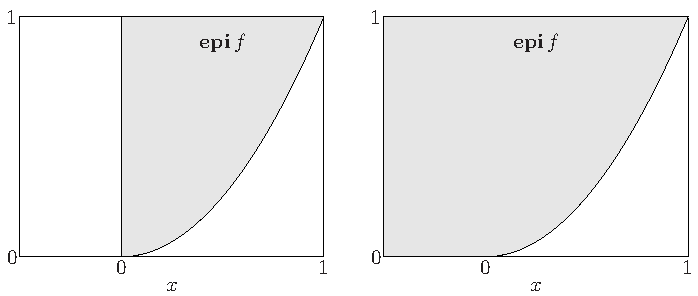
\includegraphics[width=.75\textwidth]{figures/ch03-99.pdf}
\caption*{图3.7 左：定义域为 $\R_+$ 的函数 $x^2$ 凸且在定义域上单调不减，但其扩展值延拓并不单调不减。右：定义域为 $\R$ 的函数 $\max\{x,0\}^2$ 凸，且其扩展值延拓单调不减。}
\end{figure}
复合结论(3.11)可以直接证明，不必假设可微，也不必使用公式(3.9)。例如，证明如下复合定理：若 $g$ 凸、$h$ 凸且 $\widetilde h$ 单调不减，则 $f=h\circ g$ 凸。设 $x,y\in\dom f$、$0\leq\theta\leq1$。由 $x,y\in\dom f$，有 $x,y\in\dom g$ 以及 $g(x),g(y)\in\dom h$。由于 $\dom g$ 凸，有 $\theta x+(1-\theta)y\in\dom g$，再由 $g$ 的凸性得
\begin{equation}g(\theta x+(1-\theta)y)\leq\theta g(x)+(1-\theta)g(y).\tag{3.12}\end{equation}
因为 $g(x),g(y)\in\dom h$，所以 $\theta g(x)+(1-\theta)g(y)\in\dom h$，即式(3.12)右端属于 $\dom h$。现在使用 $\widetilde h$ 单调不减这一假设，它意味着定义域沿负方向无限延伸。式(3.12)右端属于 $\dom h$，故左端 $g(\theta x+(1-\theta)y)$ 也属于 $\dom h$。这意味着 $\theta x+(1-\theta)y\in\dom f$。至此已证明 $\dom f$ 凸。

再利用 $\widetilde h$ 单调不减和不等式(3.12)，得
\begin{equation}h(g(\theta x+(1-\theta)y))\leq h(\theta g(x)+(1-\theta)g(y)).\tag{3.13}\end{equation}
由 $h$ 的凸性有
\begin{equation}h(\theta g(x)+(1-\theta)g(y))\leq\theta h(g(x))+(1-\theta)h(g(y)).\tag{3.14}\end{equation}
% Source PDF page 100 (printed p. 86)
合并式(3.13)与(3.14)，得到
\[h(g(\theta x+(1-\theta)y))\leq\theta h(g(x))+(1-\theta)h(g(y)),\]
从而证明了复合定理。
\begin{origexample}{3.13}
\textbf{简单的复合结论。}
\begin{itemize}
\item 若 $g$ 凸，则 $\exp g(x)$ 凸。
\item 若 $g$ 凹且为正，则 $\log g(x)$ 凹。
\item 若 $g$ 凹且为正，则 $1/g(x)$ 凸。
\item 若 $g$ 凸且非负、$p\geq1$，则 $g(x)^p$ 凸。
\item 若 $g$ 凸，则 $-\log(-g(x))$ 在 $\{x\mid g(x)<0\}$ 上凸。
\end{itemize}
\end{origexample}
\paragraph{注3.3}不能把扩展值延拓 $\widetilde h$ 的单调性要求，放宽为只要求函数 $h$ 单调。例如，考虑 $g(x)=x^2$、$\dom g=\R$，以及 $h(x)=0$、$\dom h=[1,2]$。这里 $g$ 凸，$h$ 凸且单调不减，但复合函数 $f=h\circ g$，即
\[f(x)=0,\qquad\dom f=[-\sqrt2,-1]\cup[1,\sqrt2],\]
不凸，因为定义域不凸。这里的 $\widetilde h$ 当然并不单调不减。

\subsubsection*{向量复合}
现在考虑更复杂的 $k\geq1$ 情形。设
\[f(x)=h(g(x))=h(g_1(x),\ldots,g_k(x)),\]
其中 $h:\R^k\to\R$、$g_i:\R^n\to\R$。仍可不失一般性地假设 $n=1$。如同 $k=1$，为发现复合规则，先假设函数二次可微，且 $\dom g=\R$、$\dom h=\R^k$。有
\begin{equation}
 f''(x)=g'(x)^\T\nabla^2h(g(x))g'(x)+\nabla h(g(x))^\T g''(x),\tag{3.15}
\end{equation}
这是式(3.9)的向量形式。问题仍是确定哪些条件可以保证对所有 $x$ 有 $f''(x)\geq0$（凹性则对应 $f''(x)\leq0$）。由式(3.15)可以导出许多规则，例如：
\begin{itemize}
\item 若 $h$ 凸、对每个自变量单调不减，且各 $g_i$ 凸，则 $f$ 凸；
\item 若 $h$ 凸、对每个自变量单调不增，且各 $g_i$ 凹，则 $f$ 凸；
\item 若 $h$ 凹、对每个自变量单调不减，且各 $g_i$ 凹，则 $f$ 凹。
\end{itemize}
% Source PDF page 101 (printed p. 87)
与标量情况一样，在 $n>1$、不假设 $h,g$ 可微、定义域一般的情况下，类似的复合结论仍成立。一般结论要求 $h$ 的单调性条件对扩展值延拓 $\widetilde h$ 成立。

为理解扩展值延拓 $\widetilde h$ 的单调性条件，考虑 $h:\R^k\to\R$ 凸，$\widetilde h$ 单调不减的情况，即只要 $u\preceq v$ 就有 $\widetilde h(u)\leq\widetilde h(v)$。这意味着，若 $v\in\dom h$，则 $u\in\dom h$：$h$ 的定义域必须沿 $-\R_+^k$ 的方向无限延伸。可以简写为 $\dom h-\R_+^k=\dom h$。
\begin{origexample}{3.14}
\textbf{向量复合的例子。}
\begin{itemize}
\item 令 $h(z)=z_{[1]}+\cdots+z_{[r]}$，即 $z\in\R^k$ 中最大的 $r$ 个分量之和。$h$ 凸且对每个自变量单调不减。设 $g_1,\ldots,g_k$ 是 $\R^n$ 上的凸函数，则复合函数 $f=h\circ g$，也就是各 $g_i$ 中最大的 $r$ 个的逐点和，凸。
\item 函数 $h(z)=\log(\sum_{i=1}^k e^{z_i})$ 凸且对每个自变量单调不减，因此只要各 $g_i$ 凸，$\log(\sum_{i=1}^k e^{g_i})$ 就凸。
\item 对 $0<p\leq1$，函数 $h(z)=(\sum_{i=1}^k z_i^p)^{1/p}$ 在 $\R_+^k$ 上凹，且其延拓（在 $z\not\succeq0$ 时取 $-\infty$）对每个分量单调不减。因此，若各 $g_i$ 凹且非负，则 $f(x)=(\sum_{i=1}^k g_i(x)^p)^{1/p}$ 凹。
\item 设 $p\geq1$，$g_1,\ldots,g_k$ 凸且非负，则函数 $(\sum_{i=1}^k g_i(x)^p)^{1/p}$ 凸。为证明这一点，考虑 $h:\R^k\to\R$，
\[h(z)=\left(\sum_{i=1}^k\max\{z_i,0\}^p\right)^{1/p},\]
其中 $\dom h=\R^k$，所以 $h=\widetilde h$。此函数凸且单调不减，故 $h(g(x))$ 关于 $x$ 凸。对 $z\succeq0$，$h(z)=(\sum_{i=1}^k z_i^p)^{1/p}$，于是得到 $(\sum_{i=1}^k g_i(x)^p)^{1/p}$ 凸。
\item 几何平均 $h(z)=(\prod_{i=1}^k z_i)^{1/k}$ 在 $\R_+^k$ 上凹，且其延拓对每个自变量单调不减。因此，若 $g_1,\ldots,g_k$ 是非负凹函数，它们的几何平均 $(\prod_{i=1}^k g_i)^{1/k}$ 也凹。
\end{itemize}
\end{origexample}
\subsection{最小化}
我们已经看到，任意一族凸函数的最大值或上确界凸。事实上，某些特殊形式的最小化也能产生凸函数。若 $f$ 关于 $(x,y)$ 凸，且 $C$ 为非空凸集，则函数
\begin{equation}g(x)=\inf_{y\in C}f(x,y)\tag{3.16}\end{equation}
% Source PDF page 102 (printed p. 88)
关于 $x$ 凸，只要对所有 $x$ 都有 $g(x)>-\infty$。$g$ 的定义域是 $\dom f$ 在 $x$ 坐标上的投影，即
\[\dom g=\{x\mid\text{存在 }y\in C\text{ 使 }(x,y)\in\dom f\}.\]
下面对 $x_1,x_2\in\dom g$ 验证 Jensen 不等式，证明这一结论。令 $\epsilon>0$。存在 $y_1,y_2\in C$，使 $f(x_i,y_i)\leq g(x_i)+\epsilon$，$i=1,2$。再令 $\theta\in[0,1]$，有
\[
\begin{aligned}
 g(\theta x_1+(1-\theta)x_2)
 &=\inf_{y\in C}f(\theta x_1+(1-\theta)x_2,y)\\
 &\leq f(\theta x_1+(1-\theta)x_2,\theta y_1+(1-\theta)y_2)\\
 &\leq\theta f(x_1,y_1)+(1-\theta)f(x_2,y_2)\\
 &\leq\theta g(x_1)+(1-\theta)g(x_2)+\epsilon.
\end{aligned}
\]
由于这对任意 $\epsilon>0$ 成立，得到
\[g(\theta x_1+(1-\theta)x_2)\leq\theta g(x_1)+(1-\theta)g(x_2).\]
这一结论也可以通过上图看出。$f,g,C$ 如式(3.16)所定义，并假设每个 $x$ 处对 $y\in C$ 的下确界都能取到，则
\[\epi g=\{(x,t)\mid\text{存在 }y\in C\text{ 使 }(x,y,t)\in\epi f\}.\]
因此 $\epi g$ 凸，因为它是凸集在部分坐标上的投影。
\begin{origexample}{3.15}
\textbf{Schur 补。}设二次函数
\[f(x,y)=x^\T Ax+2x^\T By+y^\T Cy,\]
其中 $A,C$ 对称，关于 $(x,y)$ 凸，这意味着
\[\begin{bmatrix}A&B\\B^\T&C\end{bmatrix}\succeq0.\]
可以将 $g(x)=\inf_y f(x,y)$ 表示为
\[g(x)=x^\T(A-BC^\dagger B^\T)x,\]
其中 $C^\dagger$ 是 $C$ 的伪逆（见A.5.4节）。由最小化规则，$g$ 凸，因此 $A-BC^\dagger B^\T\succeq0$。

若 $C$ 可逆，即 $C\succ0$，则矩阵 $A-BC^{-1}B^\T$ 称为 $C$ 在矩阵
\[\begin{bmatrix}A&B\\B^\T&C\end{bmatrix}\]
中的 Schur 补（见A.5.5节）。
\end{origexample}
\begin{origexample}{3.16}
\textbf{到集合的距离。}在范数 $\norm{\cdot}$ 下，点 $x$ 到集合 $S\subseteq\R^n$ 的距离定义为
\[\dist(x,S)=\inf_{y\in S}\norm{x-y}.\]
函数 $\norm{x-y}$ 关于 $(x,y)$ 凸，因此若 $S$ 凸，则距离函数 $\dist(x,S)$ 关于 $x$ 凸。
\end{origexample}
% Source PDF page 103 (printed p. 89)
\begin{origexample}{3.17}
设 $h$ 凸，则函数
\[g(x)=\inf\{h(y)\mid Ay=x\}\]
凸。为证明这一点，定义
\[f(x,y)=\begin{cases}h(y),&Ay=x,\\\infty,&\text{其他情况},\end{cases}\]
它关于 $(x,y)$ 凸。$g$ 是 $f$ 对 $y$ 的最小值，因此凸。（直接证明 $g$ 凸也并不难。）
\end{origexample}
\subsection{函数的透视}
若 $f:\R^n\to\R$，则 $f$ 的透视是函数 $g:\R^{n+1}\to\R$，定义为
\[g(x,t)=tf(x/t),\]
定义域为
\[\dom g=\{(x,t)\mid x/t\in\dom f,\ t>0\}.\]
透视运算保持凸性：若 $f$ 凸，其透视函数 $g$ 也凸。类似地，若 $f$ 凹，则 $g$ 凹。

这一结论有多种证明，例如直接验证定义不等式（见习题3.33）。这里用上图和2.3.3节介绍的 $\R^{n+1}$ 上的透视映射，给出简短证明，这也解释了“透视”一词的由来。对 $t>0$ 有
\[
\begin{aligned}
 (x,t,s)\in\epi g&\Longleftrightarrow tf(x/t)\leq s\\
 &\Longleftrightarrow f(x/t)\leq s/t\\
 &\Longleftrightarrow(x/t,s/t)\in\epi f.
\end{aligned}
\]
因此，$\epi g$ 是 $\epi f$ 在将 $(u,v,w)$ 映到 $(u,w)/v$ 的透视映射下的逆像。由2.3.3节，$\epi g$ 凸，故 $g$ 凸。
\begin{origexample}{3.18}
\textbf{欧氏范数的平方。}$\R^n$ 上凸函数 $f(x)=x^\T x$ 的透视为
\[g(x,t)=t(x/t)^\T(x/t)=\frac{x^\T x}{t},\]
当 $t>0$ 时关于 $(x,t)$ 凸。

也可以用几种其他方法推出 $g$ 凸。首先，将 $g$ 写成二次除以线性函数 $x_i^2/t$ 的和，这些函数已在3.1.5节证明为凸。也可以将 $g$ 表示为矩阵分式函数的特例 $x^\T(tI)^{-1}x$（见例3.4）。
\end{origexample}
% Source PDF page 104 (printed p. 90)
\begin{origexample}{3.19}
\textbf{负对数。}考虑 $\R_{++}$ 上的凸函数 $f(x)=-\log x$。它的透视为
\[g(x,t)=-t\log(x/t)=t\log(t/x)=t\log t-t\log x,\]
在 $\R_{++}^2$ 上凸。函数 $g$ 称为 $t$ 和 $x$ 的相对熵。当 $x=1$ 时，$g$ 成为负熵函数。

从 $g$ 的凸性可以证明几个相关函数的凸性或凹性。首先，两个向量 $u,v\in\R_{++}^n$ 的相对熵定义为
\[\sum_{i=1}^n u_i\log(u_i/v_i),\]
它关于 $(u,v)$ 凸，因为它是各对 $u_i,v_i$ 相对熵之和。

一个密切相关的函数是 $u,v\in\R_{++}^n$ 之间的 Kullback--Leibler 散度，
\begin{equation}
 D_{\mathrm{kl}}(u,v)=\sum_{i=1}^n\bigl(u_i\log(u_i/v_i)-u_i+v_i\bigr),\tag{3.17}
\end{equation}
它凸，因为它是相对熵加上 $(u,v)$ 的线性函数。Kullback--Leibler 散度满足 $D_{\mathrm{kl}}(u,v)\geq0$，且 $D_{\mathrm{kl}}(u,v)=0$ 当且仅当 $u=v$，因此可用来度量两个正向量之间的偏离程度；见习题3.13。（当 $u,v$ 为概率向量，即 $\one^\T u=\one^\T v=1$ 时，相对熵与 Kullback--Leibler 散度相同。）

在相对熵函数中取 $v_i=\one^\T u$，便得到 $u\in\R_{++}^n$ 的凹函数，而且具有齐次性：
\[\sum_{i=1}^n u_i\log(\one^\T u/u_i)=(\one^\T u)\sum_{i=1}^n z_i\log(1/z_i),\]
其中 $z=u/(\one^\T u)$，该函数称为归一化熵函数。向量 $z=u/(\one^\T u)$ 的分量和为一，是归一化向量或概率分布；$u$ 的归一化熵是此归一化分布的熵乘以 $\one^\T u$。
\end{origexample}
\begin{origexample}{3.20}
设 $f:\R^m\to\R$ 凸，$A\in\R^{m\times n}$、$b\in\R^m$、$c\in\R^n$、$d\in\R$。定义
\[g(x)=(c^\T x+d)f\bigl((Ax+b)/(c^\T x+d)\bigr),\]
定义域为
\[\dom g=\{x\mid c^\T x+d>0,\ (Ax+b)/(c^\T x+d)\in\dom f\}.\]
则 $g$ 凸。
\end{origexample}
\section{共轭函数}
本节介绍一种将在后面章节起重要作用的运算。
% Source PDF page 105 (printed p. 91)
\begin{figure}[htbp]\centering
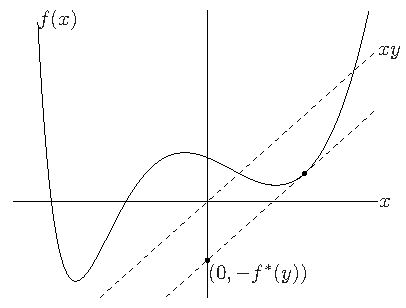
\includegraphics[width=.5\textwidth]{figures/ch03-105.pdf}
\caption*{图3.8 函数 $f:\R\to\R$ 以及一个数 $y\in\R$。共轭函数 $f^*(y)$ 是线性函数 $yx$ 与 $f(x)$ 之间的最大差距，由图中的虚线表示。若 $f$ 可微，这个最大差距在满足 $f'(x)=y$ 的点 $x$ 处取得。}
\end{figure}
\subsection{定义与例子}
设 $f:\R^n\to\R$。函数 $f^*:\R^n\to\R$，
\begin{equation}f^*(y)=\sup_{x\in\dom f}\bigl(y^\T x-f(x)\bigr),\tag{3.18}\end{equation}
称为 $f$ 的共轭函数。其定义域由使上确界有限的 $y\in\R^n$ 组成，即差 $y^\T x-f(x)$ 在 $\dom f$ 上有上界的那些 $y$。图3.8说明了这一定义。

可以立即看出，$f^*$ 凸，因为它是一族关于 $y$ 的凸函数（事实上为仿射函数）的逐点上确界。不论 $f$ 是否凸，这都成立。（当 $f$ 凸时，不必写出下标 $x\in\dom f$，因为按约定，对 $x\notin\dom f$ 有 $y^\T x-f(x)=-\infty$。）

先给出几个简单例子，再介绍一些求函数共轭的规则。这样就能导出许多常见凸函数的共轭函数的解析表达式。
\begin{origexample}{3.21}
下面求出 $\R$ 上几个凸函数的共轭。
\begin{itemize}
\item \textbf{仿射函数。}$f(x)=ax+b$。作为 $x$ 的函数，$yx-ax-b$ 有界当且仅当 $y=a$，此时它是常数。因此共轭函数 $f^*$ 的定义域为单点集 $\{a\}$，且 $f^*(a)=-b$。
\item \textbf{负对数。}$f(x)=-\log x$、$\dom f=\R_{++}$。若 $y\geq0$，函数 $xy+\log x$ 向上无界；否则在 $x=-1/y$ 处取得最大值。因此，$\dom f^*=\{y\mid y<0\}=-\R_{++}$，且对 $y<0$ 有 $f^*(y)=-\log(-y)-1$。
\item \textbf{指数。}$f(x)=e^x$。若 $y<0$，$xy-e^x$ 无界。若 $y>0$，$xy-e^x$ 在 $x=\log y$ 处取得最大值，所以 $f^*(y)=y\log y-y$。当 $y=0$ 时，
% Source PDF page 106 (printed p. 92)
$f^*(y)=\sup_x(-e^x)=0$。综上，$\dom f^*=\R_+$，$f^*(y)=y\log y-y$，其中约定 $0\log0=0$。
\item \textbf{负熵。}$f(x)=x\log x$、$\dom f=\R_+$，并令 $f(0)=0$。对所有 $y$，函数 $xy-x\log x$ 在 $\R_+$ 上有上界，因此 $\dom f^*=\R$。它在 $x=e^{y-1}$ 处取得最大值，代入得到 $f^*(y)=e^{y-1}$。
\item \textbf{倒数。}$f(x)=1/x$，定义在 $\R_{++}$ 上。当 $y>0$ 时，$yx-1/x$ 向上无界；当 $y=0$ 时，上确界为零；当 $y<0$ 时，在 $x=(-y)^{-1/2}$ 处取得上确界。因此，$f^*(y)=-2(-y)^{1/2}$，$\dom f^*=-\R_+$。
\end{itemize}
\end{origexample}
\begin{origexample}{3.22}
\textbf{严格凸二次函数。}考虑 $f(x)=\tfrac12x^\T Qx$，$Q\in\mathbb S_{++}^n$。对所有 $y$，关于 $x$ 的函数 $y^\T x-\tfrac12x^\T Qx$ 都有上界。它在 $x=Q^{-1}y$ 处取得最大值，故
\[f^*(y)=\tfrac12y^\T Q^{-1}y.\]
\end{origexample}
\begin{origexample}{3.23}
\textbf{行列式的对数。}考虑 $\mathbb S_{++}^n$ 上的 $f(X)=\log\det X^{-1}$。共轭函数定义为
\[f^*(Y)=\sup_{X\succ0}\bigl(\tr(YX)+\log\det X\bigr),\]
因为 $\tr(YX)$ 是 $\mathbb S^n$ 上的标准内积。先证明，除非 $Y\prec0$，否则 $\tr(YX)+\log\det X$ 向上无界。若 $Y\not\prec0$，则 $Y$ 有一个特征向量 $v$，满足 $\norm v_2=1$，对应特征值 $\lambda\geq0$。取 $X=I+tvv^\T$，则
\[
 \tr(YX)+\log\det X=\tr Y+t\lambda+\log\det(I+tvv^\T)
 =\tr Y+t\lambda+\log(1+t),
\]
当 $t\to\infty$ 时向上无界。

再考虑 $Y\prec0$。令关于 $X$ 的梯度为零，可以找到使目标最大的 $X$：
\[\nabla_X\bigl(\tr(YX)+\log\det X\bigr)=Y+X^{-1}=0\]
（见A.4.1节），得到 $X=-Y^{-1}$，它确实正定。因此
\[f^*(Y)=\log\det(-Y)^{-1}-n,\qquad\dom f^*=-\mathbb S_{++}^n.\]
\end{origexample}
\begin{origexample}{3.24}
\textbf{示性函数。}设 $I_S$ 为集合 $S\subseteq\R^n$（不一定凸）的示性函数，即 $I_S(x)=0$，$\dom I_S=S$。它的共轭为
\[I_S^*(y)=\sup_{x\in S}y^\T x,\]
即集合 $S$ 的支撑函数。
\end{origexample}
% Source PDF page 107 (printed p. 93)
\begin{origexample}{3.25}
\textbf{指数和对数函数。}为求 $f(x)=\log(\sum_{i=1}^n e^{x_i})$ 的共轭，先确定哪些 $y$ 能使 $y^\T x-f(x)$ 关于 $x$ 的最大值取到。令关于 $x$ 的梯度为零，得到条件
\[y_i=\frac{e^{x_i}}{\sum_{j=1}^n e^{x_j}},\qquad i=1,\ldots,n.\]
这些方程关于 $x$ 有解，当且仅当 $y\succ0$ 且 $\one^\T y=1$。把 $y_i$ 的表达式代入 $y^\T x-f(x)$，得到 $f^*(y)=\sum_{i=1}^n y_i\log y_i$。即使 $y$ 的某些分量为零，只要 $y\succeq0$、$\one^\T y=1$，并约定 $0\log0=0$，这个表达式仍成立。

事实上，$f^*$ 的定义域恰由 $\one^\T y=1$、$y\succeq0$ 给出。为证明这一点，先设 $y$ 有一个负分量，例如 $y_k<0$。取 $x_k=-t$、$x_i=0$（$i\ne k$），再令 $t\to\infty$，就能证明 $y^\T x-f(x)$ 向上无界。若 $y\succeq0$ 但 $\one^\T y\ne1$，取 $x=t\one$，有
\[y^\T x-f(x)=t\one^\T y-t-\log n.\]
若 $\one^\T y>1$，它在 $t\to\infty$ 时无界增大；若 $\one^\T y<1$，则在 $t\to-\infty$ 时无界增大。

综上，
\[f^*(y)=\begin{cases}\sum_{i=1}^n y_i\log y_i,&y\succeq0,\ \one^\T y=1,\\
 \infty,&\text{其他情况}.\end{cases}\]
换句话说，指数和对数函数的共轭，是限制在概率单纯形上的负熵函数。
\end{origexample}
\begin{origexample}{3.26}
\textbf{范数。}设 $\norm{\cdot}$ 是 $\R^n$ 上的范数，对偶范数为 $\norm{\cdot}_*$。将证明，$f(x)=\norm x$ 的共轭为
\[f^*(y)=\begin{cases}0,&\norm y_*\leq1,\\\infty,&\text{其他情况},\end{cases}\]
即范数的共轭是对偶范数单位球的示性函数。

若 $\norm y_*>1$，则由对偶范数定义，存在 $z\in\R^n$，$\norm z\leq1$，使 $y^\T z>1$。取 $x=tz$ 并令 $t\to\infty$，有
\[y^\T x-\norm x=t(y^\T z-\norm z)\to\infty,\]
表明 $f^*(y)=\infty$。反过来，若 $\norm y_*\leq1$，则对所有 $x$ 有 $y^\T x\leq\norm x\norm y_*$，从而 $y^\T x-\norm x\leq0$。因此，$x=0$ 使 $y^\T x-\norm x$ 达到最大值零。
\end{origexample}
\begin{origexample}{3.27}
\textbf{范数的平方。}现在考虑 $f(x)=\tfrac12\norm x^2$，其中 $\norm{\cdot}$ 为范数，对偶范数为 $\norm{\cdot}_*$。将证明其共轭为 $f^*(y)=\tfrac12\norm y_*^2$。由 $y^\T x\leq\norm y_*\norm x$ 得
\[y^\T x-\tfrac12\norm x^2\leq\norm y_*\norm x-\tfrac12\norm x^2\]
% Source PDF page 108 (printed p. 94)
对所有 $x$ 成立。右端是关于 $\norm x$ 的二次函数，最大值为 $\tfrac12\norm y_*^2$。因此对所有 $x$ 都有
\[y^\T x-\tfrac12\norm x^2\leq\tfrac12\norm y_*^2,\]
表明 $f^*(y)\leq\tfrac12\norm y_*^2$。

为证明另一个方向，取满足 $y^\T x=\norm y_*\norm x$ 的任意向量 $x$，并缩放至 $\norm x=\norm y_*$。对这个 $x$ 有
\[y^\T x-\tfrac12\norm x^2=\tfrac12\norm y_*^2,\]
表明 $f^*(y)\geq\tfrac12\norm y_*^2$。
\end{origexample}
\begin{origexample}{3.28}
\textbf{收入与利润函数。}考虑一家消耗 $n$ 种资源、生产可供销售产品的企业。用 $r=(r_1,\ldots,r_n)$ 表示消耗的资源数量向量，用 $S(r)$ 表示产品带来的销售收入，它是所耗资源的函数。令 $p_i$ 为第 $i$ 种资源的单位价格，则企业为资源支付的总金额为 $p^\T r$，利润为 $S(r)-p^\T r$。固定资源价格，问：通过合理选择消耗的资源数量，最多能获得多少利润？最大利润为
\[M(p)=\sup_r\bigl(S(r)-p^\T r\bigr).\]
函数 $M(p)$ 给出可达到的最大利润，作为资源价格的函数。用共轭函数可以写成
\[M(p)=(-S)^*(-p).\]
因此，最大利润（资源价格的函数）与销售总收入（所耗资源的函数）的共轭密切相关。
\end{origexample}
\subsection{基本性质}
\subsubsection*{Fenchel 不等式}
由共轭函数的定义，立即得到对所有 $x,y$ 成立的不等式
\[f(x)+f^*(y)\geq x^\T y.\]
它称为 Fenchel 不等式（当 $f$ 可微时，也称 Young 不等式）。

例如，对 $f(x)=\tfrac12x^\T Qx$、$Q\in\mathbb S_{++}^n$，得到
\[x^\T y\leq\tfrac12x^\T Qx+\tfrac12y^\T Q^{-1}y.\]
\subsubsection*{共轭的共轭}
上述例子以及“共轭”这个名称，都暗示凸函数的共轭的共轭就是原函数。满足一个技术条件时确实如此：若 $f$ 凸且闭（即 $\epi f$ 为闭集；见A.3.3节），则 $f^{**}=f$。例如，若 $\dom f=\R^n$，就有 $f^{**}=f$，即 $f$ 的共轭的共轭仍为 $f$（见习题3.39）。
% Source PDF page 109 (printed p. 95)
\subsubsection*{可微函数}
可微函数 $f$ 的共轭也称为 $f$ 的 Legendre 变换。（为区别一般定义与可微情形，有时用 Fenchel 共轭一词代替共轭。）

设 $f$ 凸且可微，$\dom f=\R^n$。使 $y^\T x-f(x)$ 最大的任意 $x^*$ 都满足 $y=\nabla f(x^*)$；反过来，若 $x^*$ 满足 $y=\nabla f(x^*)$，则 $x^*$ 使 $y^\T x-f(x)$ 最大。因此，当 $y=\nabla f(x^*)$ 时，
\[f^*(y)=x^{*\T}\nabla f(x^*)-f(x^*).\]
因此，只要对给定 $y$ 能解出梯度方程 $y=\nabla f(z)$ 中的 $z$，就能确定 $f^*(y)$。

也可以换一种表达方式：任取 $z\in\R^n$，定义 $y=\nabla f(z)$，则
\[f^*(y)=z^\T\nabla f(z)-f(z).\]
\subsubsection*{数乘及与仿射变换复合}
对 $a>0$、$b\in\R$，$g(x)=af(x)+b$ 的共轭为 $g^*(y)=af^*(y/a)-b$。

设 $A\in\R^{n\times n}$ 非奇异，$b\in\R^n$。则 $g(x)=f(Ax+b)$ 的共轭为
\[g^*(y)=f^*(A^{-\T}y)-b^\T A^{-\T}y,\qquad\dom g^*=A^\T\dom f^*.\]
\subsubsection*{相互独立函数之和}
若 $f(u,v)=f_1(u)+f_2(v)$，其中 $f_1,f_2$ 为凸函数，共轭分别为 $f_1^*,f_2^*$，则
\[f^*(w,z)=f_1^*(w)+f_2^*(z).\]
换句话说，相互独立的凸函数之和的共轭，等于各自共轭之和。（这里“相互独立”指它们是不同变量的函数。）
\section{拟凸函数}
\subsection{定义与例子}
若函数 $f:\R^n\to\R$ 的定义域以及对所有 $\alpha\in\R$ 的下水平集
\[S_\alpha=\{x\in\dom f\mid f(x)\leq\alpha\}\]
都凸，则称 $f$ 拟凸（或单峰）。若 $-f$ 拟凸，则称 $f$ 拟凹，也就是每个上水平集 $\{x\mid f(x)\geq\alpha\}$ 都凸。既拟凸又拟凹的函数称为拟线性函数。若 $f$ 拟线性，则它的定义域以及每个水平集 $\{x\mid f(x)=\alpha\}$ 都凸。
% Source PDF page 110 (printed p. 96)
\begin{figure}[htbp]\centering
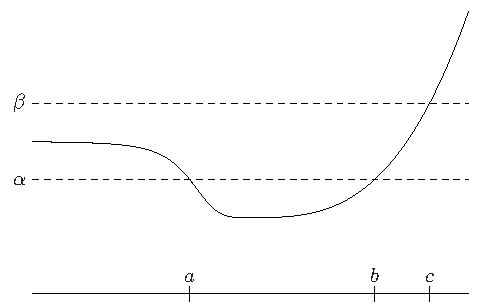
\includegraphics[width=.58\textwidth]{figures/ch03-110.pdf}
\caption*{图3.9 $\R$ 上的拟凸函数。对每个 $\alpha$，$\alpha$-下水平集 $S_\alpha$ 都凸，即为区间。下水平集 $S_\alpha$ 是 $[a,b]$，下水平集 $S_\beta$ 是 $(-\infty,c]$。}
\end{figure}
对于 $\R$ 上的函数，拟凸性要求每个下水平集都是区间，其中也可以包括无穷区间。图3.9给出了 $\R$ 上一个拟凸函数的例子。

凸函数的下水平集凸，因此凸函数都拟凸。但简单例子，例如图3.9，表明逆命题不成立。
\begin{origexample}{3.29}
$\R$ 上的几个例子：
\begin{itemize}
\item \textbf{对数。}$\R_{++}$ 上的 $\log x$ 拟凸，也拟凹，因而拟线性。
\item \textbf{向上取整函数。}$\operatorname{ceil}(x)=\inf\{z\in\Z\mid z\geq x\}$ 拟凸，也拟凹。
\end{itemize}
\end{origexample}
这些例子表明，拟凸函数可以是凹函数，也可以不连续。下面给出 $\R^n$ 上的一些例子。
\begin{origexample}{3.30}
\textbf{向量的长度。}将 $x\in\R^n$ 的长度定义为非零分量的最大下标，即
\[f(x)=\max\{i\mid x_i\ne0\}.\]
（规定零向量的长度为零。）此函数在 $\R^n$ 上拟凸，因为它的下水平集是子空间：
\[f(x)\leq\alpha\ \Longleftrightarrow\ x_i=0,\quad i=\lfloor\alpha\rfloor+1,\ldots,n.\]
\end{origexample}
\begin{origexample}{3.31}
考虑 $f:\R^2\to\R$，$\dom f=\R_+^2$，$f(x_1,x_2)=x_1x_2$。它既不凸也不凹，因为 Hessian
\[\nabla^2f(x)=\begin{bmatrix}0&1\\1&0\end{bmatrix}\]
% Source PDF page 111 (printed p. 97)
不定，有一个正特征值和一个负特征值。不过，$f$ 拟凹，因为对所有 $\alpha$，上水平集
\[\{x\in\R_+^2\mid x_1x_2\geq\alpha\}\]
都凸。（但 $f$ 在 $\R^2$ 上不拟凹。）
\end{origexample}
\begin{origexample}{3.32}
\textbf{线性分式函数。}函数
\[f(x)=\frac{a^\T x+b}{c^\T x+d},\qquad\dom f=\{x\mid c^\T x+d>0\},\]
既拟凸又拟凹，即拟线性。它的 $\alpha$-下水平集为
\[
\begin{aligned}
 S_\alpha&=\{x\mid c^\T x+d>0,\ (a^\T x+b)/(c^\T x+d)\leq\alpha\}\\
 &=\{x\mid c^\T x+d>0,\ a^\T x+b\leq\alpha(c^\T x+d)\},
\end{aligned}
\]
它凸，因为它是一个开半空间和一个闭半空间的交。（同样可以证明上水平集凸。）
\end{origexample}
\begin{origexample}{3.33}
\textbf{距离比函数。}设 $a,b\in\R^n$，定义
\[f(x)=\frac{\norm{x-a}_2}{\norm{x-b}_2},\]
即到 $a$ 的欧氏距离与到 $b$ 的欧氏距离之比。那么，$f$ 在半空间 $\{x\mid\norm{x-a}_2\leq\norm{x-b}_2\}$ 上拟凸。为证明这一点，考虑 $f$ 的 $\alpha$-下水平集，其中取 $\alpha\leq1$，因为在上述半空间上 $f(x)\leq1$。这个下水平集由满足
\[\norm{x-a}_2\leq\alpha\norm{x-b}_2\]
的点组成。两边平方并整理，可见它等价于
\[(1-\alpha^2)x^\T x-2(a-\alpha^2b)^\T x+a^\T a-\alpha^2b^\T b\leq0.\]
当 $\alpha\leq1$ 时，这描述了一个凸集，事实上是一个欧氏球。
\end{origexample}
\begin{origexample}{3.34}
\textbf{内部收益率。}用 $x=(x_0,x_1,\ldots,x_n)$ 表示跨越 $n$ 个时期的现金流序列，其中 $x_i>0$ 表示第 $i$ 期收到的款项，$x_i<0$ 表示第 $i$ 期支付的款项。利率为 $r\geq0$ 时，现金流的现值定义为
\[\operatorname{PV}(x,r)=\sum_{i=0}^n(1+r)^{-i}x_i.\]
（因子 $(1+r)^{-i}$ 是第 $i$ 期支付或收到款项的贴现因子。）

现在考虑满足 $x_0<0$、$x_0+x_1+\cdots+x_n>0$ 的现金流。这意味着在第零期先投资 $|x_0|$，其余现金流之和 $x_1+\cdots+x_n$，在不计贴现的情况下，超过初始投资。
% Source PDF page 112 (printed p. 98)
对于这样的现金流，$\operatorname{PV}(x,0)>0$，而 $r\to\infty$ 时 $\operatorname{PV}(x,r)\to x_0<0$，因此至少存在一个 $r\geq0$ 使 $\operatorname{PV}(x,r)=0$。将现金流的内部收益率定义为使现值为零的最小非负利率：
\[\operatorname{IRR}(x)=\inf\{r\geq0\mid\operatorname{PV}(x,r)=0\}.\]
内部收益率关于 $x$ 拟凹，这里限制 $x_0<0$、$x_1+\cdots+x_n>0$。注意到
\[\operatorname{IRR}(x)\geq R\ \Longleftrightarrow\
 \operatorname{PV}(x,r)>0\text{ 对 }0\leq r<R\text{ 成立}.\]
左端定义了 IRR 的 $R$-上水平集。右端是在 $0\leq r<R$ 范围内，以 $r$ 为指标的集合 $\{x\mid\operatorname{PV}(x,r)>0\}$ 的交。对每个 $r$，$\operatorname{PV}(x,r)>0$ 定义一个开半空间，因此右端为凸集。
\end{origexample}
\subsection{基本性质}
上述例子表明，拟凸性大大推广了凸性。尽管如此，凸函数的许多性质仍然适用于拟凸函数，或者有对应的形式。例如，有一个刻画拟凸性的 Jensen 不等式变体：函数 $f$ 拟凸，当且仅当 $\dom f$ 凸，并且对任意 $x,y\in\dom f$、$0\leq\theta\leq1$，有
\begin{equation}f(\theta x+(1-\theta)y)\leq\max\{f(x),f(y)\},\tag{3.19}\end{equation}
也就是说，线段上函数值不超过两端函数值的最大值。式(3.19)有时称为拟凸函数的 Jensen 不等式，图3.10说明了这一点。
\begin{origexample}{3.35}
\textbf{非负向量的基数。}向量 $x\in\R^n$ 的基数或大小是非零分量的个数，记为 $\operatorname{card}(x)$。函数 $\operatorname{card}$ 在 $\R_+^n$ 上拟凹，但在 $\R^n$ 上不拟凹。由对 $x,y\succeq0$ 成立的修正 Jensen 不等式
\[\operatorname{card}(x+y)\geq\min\{\operatorname{card}(x),\operatorname{card}(y)\}\]
可立即得出这一点。
\end{origexample}
\begin{origexample}{3.36}
\textbf{半正定矩阵的秩。}函数 $\rank X$ 在 $\mathbb S_+^n$ 上拟凹。这来自对 $X,Y\in\mathbb S_+^n$ 成立的修正 Jensen 不等式(3.19)：
\[\rank(X+Y)\geq\min\{\rank X,\rank Y\}.\]
它可以视为上一个例子的推广，因为对 $x\succeq0$ 有 $\rank(\diag(x))=\operatorname{card}(x)$。
\end{origexample}
% Source PDF page 113 (printed p. 99)
\begin{figure}[htbp]\centering
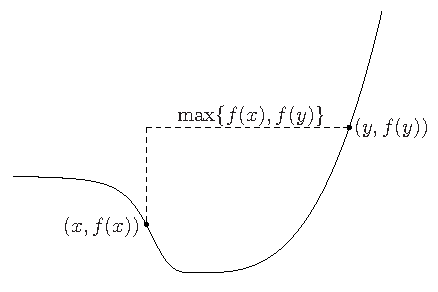
\includegraphics[width=.52\textwidth]{figures/ch03-113.pdf}
\caption*{图3.10 $\R$ 上的拟凸函数。在 $x$ 和 $y$ 之间，$f$ 的值不超过 $\max\{f(x),f(y)\}$。}
\end{figure}
如同凸性，拟凸性也由函数 $f$ 在直线上的表现刻画：$f$ 拟凸，当且仅当它在任意与定义域相交的直线上的限制拟凸。特别地，可以把函数限制在任意直线上，再检验所得 $\R$ 上函数的拟凸性，以验证原函数拟凸。
\subsubsection*{$\R$ 上的拟凸函数}
可以简单地刻画 $\R$ 上的拟凸函数。这里考虑连续函数，因为一般情况下条件的表述比较繁琐。连续函数 $f:\R\to\R$ 拟凸，当且仅当下列条件至少有一个成立：
\begin{itemize}
\item $f$ 单调不减；
\item $f$ 单调不增；
\item 存在 $c\in\dom f$，当 $t\leq c$ 且 $t\in\dom f$ 时，$f$ 单调不增；当 $t\geq c$ 且 $t\in\dom f$ 时，$f$ 单调不减。
\end{itemize}
点 $c$ 可选为 $f$ 的任意全局最小点，见图3.11。
\subsection{可微拟凸函数}
\subsubsection*{一阶条件}
设 $f:\R^n\to\R$ 可微。那么，$f$ 拟凸，当且仅当 $\dom f$ 凸，且对所有 $x,y\in\dom f$ 有
\begin{equation}f(y)\leq f(x)\ \Longrightarrow\ \nabla f(x)^\T(y-x)\leq0.\tag{3.20}\end{equation}
% Source PDF page 114 (printed p. 100)
\begin{figure}[htbp]\centering
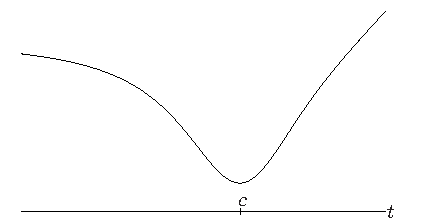
\includegraphics[width=.56\textwidth]{figures/ch03-114a.pdf}
\caption*{图3.11 $\R$ 上的拟凸函数。当 $t\leq c$ 时函数单调不增，当 $t\geq c$ 时单调不减。}
\end{figure}
\begin{figure}[htbp]\centering
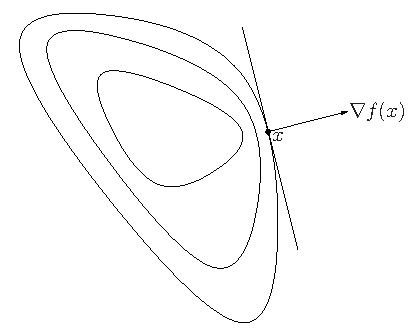
\includegraphics[width=.52\textwidth]{figures/ch03-114b.pdf}
\caption*{图3.12 拟凸函数 $f$ 的三条等高线。向量 $\nabla f(x)$ 确定了下水平集 $\{z\mid f(z)\leq f(x)\}$ 在 $x$ 处的一个支撑超平面。}
\end{figure}
这是不等式(3.2)对拟凸函数的对应形式。证明留作习题3.43。

当 $\nabla f(x)\ne0$ 时，条件(3.20)有一个简单的几何解释：$\nabla f(x)$ 确定下水平集 $\{y\mid f(y)\leq f(x)\}$ 在点 $x$ 处的支撑超平面，见图3.12。

虽然凸性的一阶条件(3.2)与拟凸性的一阶条件(3.20)相似，二者仍有重要差别。例如，若 $f$ 凸且 $\nabla f(x)=0$，则 $x$ 是 $f$ 的全局最小点。但对拟凸函数，这个命题不成立：可能有 $\nabla f(x)=0$，而 $x$ 不是 $f$ 的全局最小点。
% Source PDF page 115 (printed p. 101)
\subsubsection*{二阶条件}
现在设 $f$ 二次可微。若 $f$ 拟凸，则对所有 $x\in\dom f$ 和所有 $y\in\R^n$，有
\begin{equation}y^\T\nabla f(x)=0\ \Longrightarrow\ y^\T\nabla^2f(x)y\geq0.\tag{3.21}\end{equation}
对于 $\R$ 上的拟凸函数，这简化为
\[f'(x)=0\ \Longrightarrow\ f''(x)\geq0,\]
即斜率为零的任意一点，二阶导数非负。对 $\R^n$ 上的拟凸函数，条件(3.21)的解释稍复杂。与 $n=1$ 相同，只要 $\nabla f(x)=0$，就必须有 $\nabla^2f(x)\succeq0$。当 $\nabla f(x)\ne0$ 时，条件(3.21)意味着 $\nabla^2f(x)$ 在 $(n-1)$ 维子空间 $\nabla f(x)^\perp$ 上半正定。这说明 $\nabla^2f(x)$ 至多有一个负特征值。

作为一个部分逆命题，若 $f$ 对所有 $x\in\dom f$ 和所有 $y\in\R^n$、$y\ne0$ 都满足
\begin{equation}y^\T\nabla f(x)=0\ \Longrightarrow\ y^\T\nabla^2f(x)y>0,\tag{3.22}\end{equation}
则 $f$ 拟凸。这一条件相当于要求：在 $\nabla f(x)=0$ 的点，$\nabla^2f(x)$ 正定；在其他点，$\nabla^2f(x)$ 在 $(n-1)$ 维子空间 $\nabla f(x)^\perp$ 上正定。
\subsubsection*{拟凸性二阶条件的证明}
将函数限制在任意直线上后，只需考虑 $f:\R\to\R$。

先证明，若 $f:\R\to\R$ 在区间 $(a,b)$ 上拟凸，就必须满足式(3.21)，即若 $c\in(a,b)$、$f'(c)=0$，则 $f''(c)\geq0$。若 $f'(c)=0$、$f''(c)<0$，则对充分小的正数 $\epsilon$ 有 $f(c-\epsilon)<f(c)$、$f(c+\epsilon)<f(c)$。因此，对充分小的正数 $\epsilon$，下水平集 $\{x\mid f(x)\leq f(c)-\epsilon\}$ 不连通，从而不凸，与 $f$ 拟凸的假设矛盾。

再证明，若条件(3.22)成立，则 $f$ 拟凸。假设式(3.22)成立，即对每个满足 $f'(c)=0$ 的 $c\in(a,b)$，都有 $f''(c)>0$。这意味着，每当函数 $f'$ 穿过零值时，它严格增加，因此至多穿过零值一次。若 $f'$ 完全不穿过零值，则 $f$ 在 $(a,b)$ 上单调不增或单调不减，所以拟凸。否则，必恰好在某个 $c\in(a,b)$ 处穿过零。由于 $f''(c)>0$，有 $f'(t)\leq0$ 对 $a<t\leq c$ 成立，$f'(t)\geq0$ 对 $c\leq t<b$ 成立。这表明 $f$ 拟凸。
\subsection{保持拟凸性的运算}
\subsubsection*{非负加权最大值}
拟凸函数的非负加权最大值，即
\[f=\max\{w_1f_1,\ldots,w_mf_m\},\]
% Source PDF page 116 (printed p. 102)
其中 $w_i\geq0$、各 $f_i$ 拟凸，仍拟凸。这个性质可推广到一般的逐点上确界
\[f(x)=\sup_{y\in C}\bigl(w(y)g(x,y)\bigr),\]
其中 $w(y)\geq0$，且对每个 $y$，$g(x,y)$ 关于 $x$ 拟凸。这个事实容易验证：$f(x)\leq\alpha$ 当且仅当
\[w(y)g(x,y)\leq\alpha\qquad\text{对所有 }y\in C,\]
即 $f$ 的 $\alpha$-下水平集是各个关于变量 $x$ 的函数 $w(y)g(x,y)$ 的 $\alpha$-下水平集之交。
\begin{origexample}{3.37}
\textbf{广义特征值。}对称矩阵对 $(X,Y)$（$Y\succ0$）的最大广义特征值定义为
\[\lambda_{\max}(X,Y)=\sup_{u\ne0}\frac{u^\T Xu}{u^\T Yu}
 =\sup\{\lambda\mid\det(\lambda Y-X)=0\}.\]
见A.5.3节。此函数在 $\dom f=\mathbb S^n\times\mathbb S_{++}^n$ 上拟凸。

考虑表达式
\[\lambda_{\max}(X,Y)=\sup_{u\ne0}\frac{u^\T Xu}{u^\T Yu}.\]
对每个 $u\ne0$，$u^\T Xu/u^\T Yu$ 都是 $(X,Y)$ 的线性分式函数，从而关于 $(X,Y)$ 拟凸。因此，$\lambda_{\max}$ 作为一族拟凸函数的上确界，也拟凸。
\end{origexample}
\subsubsection*{复合}
若 $g:\R^n\to\R$ 拟凸、$h:\R\to\R$ 单调不减，则 $f=h\circ g$ 拟凸。

拟凸函数与仿射变换或线性分式变换复合，所得函数拟凸。若 $f$ 拟凸，则 $g(x)=f(Ax+b)$ 拟凸；$\widetilde g(x)=f((Ax+b)/(c^\T x+d))$ 在集合
\[\{x\mid c^\T x+d>0,\ (Ax+b)/(c^\T x+d)\in\dom f\}\]
上拟凸。
\subsubsection*{最小化}
若 $f(x,y)$ 关于 $x,y$ 联合拟凸，且 $C$ 为凸集，则函数
\[g(x)=\inf_{y\in C}f(x,y)\]
拟凸。

为证明这一点，只需证明任意 $\alpha\in\R$ 对应的 $\{x\mid g(x)\leq\alpha\}$ 凸。由 $g$ 的定义，$g(x)\leq\alpha$ 当且仅当对任意 $\epsilon>0$，都存在 $y\in C$ 使 $f(x,y)\leq\alpha+\epsilon$。
% Source PDF page 117 (printed p. 103)
设 $x_1,x_2$ 为 $g$ 的 $\alpha$-下水平集中的两点。对任意 $\epsilon>0$，存在 $y_1,y_2\in C$ 使
\[f(x_1,y_1)\leq\alpha+\epsilon,\qquad f(x_2,y_2)\leq\alpha+\epsilon.\]
因为 $f$ 关于 $x,y$ 拟凸，对 $0\leq\theta\leq1$ 还有
\[f(\theta x_1+(1-\theta)x_2,\theta y_1+(1-\theta)y_2)\leq\alpha+\epsilon.\]
因此 $g(\theta x_1+(1-\theta)x_2)\leq\alpha$，证明了 $\{x\mid g(x)\leq\alpha\}$ 凸。
\subsection{用一族凸函数表示}
后面将用到拟凸函数 $f$ 的下水平集的表示：这些集合凸，可以用凸函数的不等式描述。我们寻找一族以 $t\in\R$ 为指标的凸函数 $\phi_t:\R^n\to\R$，满足
\begin{equation}f(x)\leq t\ \Longleftrightarrow\ \phi_t(x)\leq0,\tag{3.23}\end{equation}
即拟凸函数 $f$ 的 $t$-下水平集是凸函数 $\phi_t$ 的零下水平集。显然，$\phi_t$ 必须满足：对所有 $x\in\R^n$，$\phi_t(x)\leq0$ 蕴含 $s\geq t$ 时 $\phi_s(x)\leq0$。若对每个 $x$，$\phi_t(x)$ 关于 $t$ 单调不增，即 $s\geq t$ 时 $\phi_s(x)\leq\phi_t(x)$，就满足这一性质。

为了说明这样的表示总存在，可取
\[\phi_t(x)=\begin{cases}0,&f(x)\leq t,\\\infty,&\text{其他情况},\end{cases}\]
即 $\phi_t$ 是 $f$ 的 $t$-下水平集的示性函数。显然表示不唯一；例如，若 $f$ 的下水平集闭，可取
\[\phi_t(x)=\dist\bigl(x,\{z\mid f(z)\leq t\}\bigr).\]
我们通常希望 $\phi_t$ 具有良好性质，例如可微性。
\begin{origexample}{3.38}
\textbf{凸函数除以凹函数。}设 $p$ 凸、$q$ 凹，并在凸集 $C$ 上满足 $p(x)\geq0$、$q(x)>0$。则定义在 $C$ 上的函数 $f(x)=p(x)/q(x)$ 拟凸。

因为
\[f(x)\leq t\ \Longleftrightarrow\ p(x)-tq(x)\leq0,\]
可以在 $t\geq0$ 时取 $\phi_t(x)=p(x)-tq(x)$。对每个 $t$，$\phi_t$ 凸；对每个 $x$，$\phi_t(x)$ 随 $t$ 递减。
\end{origexample}
% Source PDF page 118 (printed p. 104)
\section{对数凹函数与对数凸函数}
\subsection{定义}
若函数 $f:\R^n\to\R$ 对所有 $x\in\dom f$ 满足 $f(x)>0$，且 $\log f$ 凹，则称 $f$ 对数凹。若 $\log f$ 凸，则称它对数凸。因此，$f$ 对数凸，当且仅当 $1/f$ 对数凹。也可以方便地允许 $f$ 取零值，此时约定 $\log f(x)=-\infty$；在这种情况下，若扩展值函数 $\log f$ 凹，仍称 $f$ 对数凹。

对数凹性也可以不用对数而直接表达：定义域凸、且在定义域上恒正的函数 $f:\R^n\to\R$ 对数凹，当且仅当对所有 $x,y\in\dom f$、$0\leq\theta\leq1$，有
\[f(\theta x+(1-\theta)y)\geq f(x)^\theta f(y)^{1-\theta}.\]
特别地，对数凹函数在两点平均值处的函数值，至少为这两点函数值的几何平均。

由复合规则，若 $h$ 凸，则 $e^h$ 凸，因此对数凸函数是凸函数。类似地，非负凹函数对数凹。由于对数单调增加，对数凸函数显然拟凸，对数凹函数显然拟凹。
\begin{origexample}{3.39}
对数凹函数和对数凸函数的几个简单例子。
\begin{itemize}
\item \textbf{仿射函数。}$f(x)=a^\T x+b$ 在 $\{x\mid a^\T x+b>0\}$ 上对数凹。
\item \textbf{幂。}$\R_{++}$ 上的 $f(x)=x^a$，当 $a\leq0$ 时对数凸，当 $a\geq0$ 时对数凹。
\item \textbf{指数。}$f(x)=e^{ax}$ 既对数凸又对数凹。
\item 高斯密度的累积分布函数
\[\Phi(x)=\frac1{\sqrt{2\pi}}\int_{-\infty}^x e^{-u^2/2}\,du\]
对数凹（见习题3.54）。
\item \textbf{Gamma 函数。}Gamma 函数
\[\Gamma(x)=\int_0^\infty u^{x-1}e^{-u}\,du\]
在 $x\geq1$ 时对数凸（见习题3.52）。
\item \textbf{行列式。}$\det X$ 在 $\mathbb S_{++}^n$ 上对数凹。
\item \textbf{行列式除以迹。}$\det X/\tr X$ 在 $\mathbb S_{++}^n$ 上对数凹（见习题3.49）。
\end{itemize}
\end{origexample}
\begin{origexample}{3.40}
\textbf{对数凹密度函数。}许多常见的概率密度函数对数凹。两个例子是多元正态分布
\[f(x)=\frac1{\sqrt{(2\pi)^n\det\Sigma}}
 e^{-\frac12(x-\bar x)^\T\Sigma^{-1}(x-\bar x)}\]
% Source PDF page 119 (printed p. 105)
其中 $\bar x\in\R^n$、$\Sigma\in\mathbb S_{++}^n$，以及 $\R_+^n$ 上的指数分布
\[f(x)=\left(\prod_{i=1}^n\lambda_i\right)e^{-\lambda^\T x},\]
其中 $\lambda\succ0$。另一个例子是凸集 $C$ 上的均匀分布，
\[f(x)=\begin{cases}1/\alpha,&x\in C,\\0,&x\notin C,\end{cases}\]
其中 $\alpha=\vol(C)$ 是 $C$ 的体积，即 Lebesgue 测度。此时，$\log f$ 在 $C$ 外取 $-\infty$，在 $C$ 上取 $-\log\alpha$，因此凹。

再看一个较少见的例子，Wishart 分布。其定义如下：设 $x_1,\ldots,x_p\in\R^n$ 是独立高斯随机向量，均值为零、协方差为 $\Sigma\in\mathbb S^n$，其中 $p>n$。随机矩阵 $X=\sum_{i=1}^p x_ix_i^\T$ 的 Wishart 密度为
\[f(X)=a(\det X)^{(p-n-1)/2}e^{-\frac12\tr(\Sigma^{-1}X)},\]
$\dom f=\mathbb S_{++}^n$，$a$ 为正常数。Wishart 密度对数凹，因为
\[\log f(X)=\log a+\frac{p-n-1}2\log\det X-\frac12\tr(\Sigma^{-1}X)\]
是 $X$ 的凹函数。
\end{origexample}
\subsection{性质}
\subsubsection*{二次可微的对数凸函数与对数凹函数}
设 $f$ 二次可微，$\dom f$ 凸，则
\[\nabla^2\log f(x)=\frac1{f(x)}\nabla^2 f(x)
 -\frac1{f(x)^2}\nabla f(x)\nabla f(x)^\T.\]
因此，$f$ 对数凸，当且仅当对所有 $x\in\dom f$ 有
\[f(x)\nabla^2 f(x)\succeq\nabla f(x)\nabla f(x)^\T;\]
$f$ 对数凹，当且仅当对所有 $x\in\dom f$ 有
\[f(x)\nabla^2 f(x)\preceq\nabla f(x)\nabla f(x)^\T.\]
\subsubsection*{乘法、加法与积分}
对数凸性和对数凹性在乘法与正数乘法下封闭。例如，若 $f,g$ 对数凹，则逐点乘积 $h(x)=f(x)g(x)$ 也对数凹，因为 $\log h(x)=\log f(x)+\log g(x)$，且 $\log f(x)$、$\log g(x)$ 都是 $x$ 的凹函数。

简单例子表明，对数凹函数之和一般不对数凹。不过，加法保持对数凸性。设 $f,g$ 对数凸，即 $F=\log f$、$G=\log g$ 凸。由凸函数的复合规则，
\[\log(\exp F+\exp G)=\log(f+g)\]
% Source PDF page 120 (printed p. 106)
凸。因此，两个对数凸函数之和对数凸。

更一般地，若对每个 $y\in C$，$f(x,y)$ 关于 $x$ 对数凸，则
\[g(x)=\int_C f(x,y)\,dy\]
对数凸。
\begin{origexample}{3.41}
\textbf{非负函数的 Laplace 变换、矩母函数与累积量母函数。}设 $p:\R^n\to\R$ 对所有 $x$ 满足 $p(x)\geq0$。$p$ 的 Laplace 变换
\[P(z)=\int p(x)e^{-z^\T x}\,dx\]
在 $\R^n$ 上对数凸。（自然地，$\dom P=\{z\mid P(z)<\infty\}$。）

再设 $p$ 是密度，即 $\int p(x)\,dx=1$。函数 $M(z)=P(-z)$ 称为该密度的矩母函数。其名称来自：在 $z=0$ 处计算矩母函数的导数，即可得到密度的各阶矩。例如，
\[\nabla M(0)=\E v,\qquad\nabla^2M(0)=\E vv^\T,\]
其中 $v$ 是密度为 $p$ 的随机变量。

凸函数 $\log M(z)$ 称为 $p$ 的累积量母函数，因为它的导数给出密度的累积量。例如，累积量母函数在零处的一阶、二阶导数，分别为相关随机变量的均值和协方差：
\[\nabla\log M(0)=\E v,\qquad
 \nabla^2\log M(0)=\E(v-\E v)(v-\E v)^\T.\]
\end{origexample}
\subsubsection*{对数凹函数的积分}
在某些特殊情况下，积分保持对数凹性。若 $f:\R^n\times\R^m\to\R$ 对数凹，则
\[g(x)=\int f(x,y)\,dy\]
是 $x$ 的对数凹函数，定义在 $\R^n$ 上。这里积分在 $\R^m$ 上进行。这个结论的证明并不简单，见参考文献。

这个结论有许多重要推论，本节余下部分将介绍其中一些。例如，它说明对数凹概率密度的边缘分布仍对数凹，也说明对数凹性在卷积下封闭：若 $f,g$ 在 $\R^n$ 上对数凹，则卷积
\[(f*g)(x)=\int f(x-y)g(y)\,dy\]
也对数凹。因为 $g(y)$ 和 $f(x-y)$ 关于 $(x,y)$ 对数凹，所以乘积 $f(x-y)g(y)$ 也对数凹，再应用积分结论即可。
% Source PDF page 121 (printed p. 107)
设 $C\subseteq\R^n$ 是凸集，$w$ 为 $\R^n$ 中的随机向量，具有对数凹概率密度 $p$。则函数
\[f(x)=\Prob(x+w\in C)\]
关于 $x$ 对数凹。将 $f$ 表示为
\[f(x)=\int g(x+w)p(w)\,dw,\]
其中
\[g(u)=\begin{cases}1,&u\in C,\\0,&u\notin C,\end{cases}\]
对数凹，再应用积分结论即可。
\begin{origexample}{3.42}
概率密度函数 $f:\R^n\to\R$ 的累积分布函数定义为
\[F(x)=\Prob(w\preceq x)=\int_{-\infty}^{x_n}\cdots\int_{-\infty}^{x_1}
 f(z)\,dz_1\cdots dz_n,\]
其中 $w$ 是密度为 $f$ 的随机变量。若 $f$ 对数凹，则 $F$ 对数凹。前面已经遇到一个特例：高斯随机变量的累积分布函数
\[f(x)=\frac1{\sqrt{2\pi}}\int_{-\infty}^x e^{-t^2/2}\,dt\]
对数凹，见例3.39和习题3.54。
\end{origexample}
\begin{origexample}{3.43}
\textbf{成品率函数。}用 $x\in\R^n$ 表示生产某种产品时一组参数的标称值或目标值。制造过程的波动使产品生产出来后的参数成为 $x+w$，其中随机向量 $w\in\R^n$ 表示制造波动，通常假设均值为零。制造过程的成品率作为标称参数值的函数，为
\[Y(x)=\Prob(x+w\in S),\]
其中 $S\subseteq\R^n$ 是产品可接受参数值的集合，即产品规格。

若制造误差 $w$ 的密度对数凹，例如高斯密度，并且产品规格集合 $S$ 凸，则成品率函数 $Y$ 对数凹。这意味着 $\alpha$-成品率区域，即成品率超过 $\alpha$ 的标称参数集合，凸。例如，95\% 成品率区域
\[\{x\mid Y(x)\geq0.95\}=\{x\mid\log Y(x)\geq\log0.95\}\]
凸，因为它是凹函数 $\log Y$ 的上水平集。
\end{origexample}
% Source PDF page 122 (printed p. 108)
\begin{origexample}{3.44}
\textbf{多面体的体积。}设 $A\in\R^{m\times n}$，定义
\[P_u=\{x\in\R^n\mid Ax\preceq u\}.\]
则它的体积 $\vol P_u$ 是 $u$ 的对数凹函数。

注意函数
\[\Psi(x,u)=\begin{cases}1,&Ax\preceq u,\\0,&\text{其他情况},\end{cases}\]
对数凹。由积分结论，
\[\int\Psi(x,u)\,dx=\vol P_u\]
对数凹。
\end{origexample}
\section{相对于广义不等式的凸性}
现在用广义不等式代替 $\R$ 上的通常次序，推广单调性和凸性的概念。
\subsection{相对于广义不等式的单调性}
设 $K\subseteq\R^n$ 是正常锥，对应广义不等式 $\preceq_K$。若函数 $f:\R^n\to\R$ 满足
\[x\preceq_K y\ \Longrightarrow\ f(x)\leq f(y),\]
则称它为 $K$-单调不减函数；若满足
\[x\preceq_K y,\ x\ne y\ \Longrightarrow\ f(x)<f(y),\]
则称它为 $K$-严格递增函数。类似地定义 $K$-单调不增和 $K$-严格递减函数。
\begin{origexample}{3.45}
\textbf{向量的单调函数。}函数 $f:\R^n\to\R$ 相对于 $\R_+^n$ 单调不减，当且仅当对所有 $x,y$，有
\[x_1\leq y_1,\ldots,x_n\leq y_n\ \Longrightarrow\ f(x)\leq f(y).\]
这等同于：将 $f$ 限制在任一分量 $x_i$ 上，即把 $x_i$ 作为变量、固定 $j\ne i$ 的各 $x_j$ 时，所得函数单调不减。
\end{origexample}
\begin{origexample}{3.46}
\textbf{矩阵单调函数。}若函数 $f:\mathbb S^n\to\R$ 相对于半正定锥单调，则称它为矩阵单调函数，对应地有矩阵递增、矩阵递减。关于变量 $X\in\mathbb S^n$ 的几个矩阵单调函数例子如下：
% Source PDF page 123 (printed p. 109)
\begin{itemize}
\item $\tr(WX)$，其中 $W\in\mathbb S^n$。若 $W\succeq0$，它矩阵单调不减；若 $W\succ0$，它矩阵严格递增；若 $W\preceq0$，它矩阵单调不增；若 $W\prec0$，它矩阵严格递减。
\item $\tr(X^{-1})$ 在 $\mathbb S_{++}^n$ 上矩阵严格递减。
\item $\det X$ 在 $\mathbb S_{++}^n$ 上矩阵严格递增，在 $\mathbb S_+^n$ 上矩阵单调不减。
\end{itemize}
\end{origexample}
\subsubsection*{单调性的梯度条件}
回顾：具有凸定义域（即区间）的可微函数 $f:\R\to\R$ 单调不减，当且仅当对所有 $x\in\dom f$ 有 $f'(x)\geq0$；若所有点都有 $f'(x)>0$，则函数严格递增，但逆命题不成立。这些条件容易推广到相对于广义不等式的单调性。具有凸定义域的可微函数 $f$ 为 $K$-单调不减函数，当且仅当对所有 $x\in\dom f$ 有
\begin{equation}\nabla f(x)\succeq_{K^*}0.\tag{3.24}\end{equation}
与简单标量情形的区别是：梯度必须在对偶不等式意义下非负。严格情形有如下结论：若对所有 $x\in\dom f$ 有
\begin{equation}\nabla f(x)\succ_{K^*}0,\tag{3.25}\end{equation}
则 $f$ 为 $K$-严格递增函数。如同标量情形，逆命题不成立。

下面证明这些单调性一阶条件。先假设 $f$ 对所有 $x$ 满足式(3.24)，但不为 $K$-单调不减函数，即存在 $x,y$，$x\preceq_K y$ 且 $f(y)<f(x)$。由可微性，存在 $t\in[0,1]$ 使
\[\frac d{dt}f(x+t(y-x))=\nabla f(x+t(y-x))^\T(y-x)<0.\]
因为 $y-x\in K$，这意味着
\[\nabla f(x+t(y-x))\notin K^*,\]
与式(3.24)处处成立的假设矛盾。同样可以证明，式(3.25)蕴含 $f$ 为 $K$-严格递增函数。

式(3.24)处处成立的必要性也容易看出。假设式(3.24)在 $x=z$ 处不成立。由对偶锥定义，存在 $v\in K$ 使
\[\nabla f(z)^\T v<0.\]
考虑关于 $t$ 的函数 $h(t)=f(z+tv)$，有 $h'(0)=\nabla f(z)^\T v<0$，所以存在 $t>0$，使 $h(t)=f(z+tv)<h(0)=f(z)$，即 $f$ 不是 $K$-单调不减函数。
\subsection{相对于广义不等式的凸性}
设 $K\subseteq\R^m$ 为正常锥，对应广义不等式 $\preceq_K$。若对所有 $x,y$ 以及 $0\leq\theta\leq1$，有
\[f(\theta x+(1-\theta)y)\preceq_K\theta f(x)+(1-\theta)f(y),\]
则称 $f:\R^n\to\R^m$ 为 $K$-凸函数。
% Source PDF page 124 (printed p. 110)
若对所有 $x\ne y$、$0<\theta<1$，有
\[f(\theta x+(1-\theta)y)\prec_K\theta f(x)+(1-\theta)f(y),\]
则称为严格 $K$-凸函数。当 $m=1$、$K=\R_+$ 时，这些定义退化为通常的凸性和严格凸性。
\begin{origexample}{3.47}
\textbf{相对于逐分量不等式的凸性。}函数 $f:\R^n\to\R^m$ 相对于逐分量不等式（即 $\R_+^m$ 诱导的广义不等式）凸，当且仅当对所有 $x,y$、$0\leq\theta\leq1$ 有
\[f(\theta x+(1-\theta)y)\preceq\theta f(x)+(1-\theta)f(y),\]
即每个分量 $f_i$ 都是凸函数。函数 $f$ 相对于逐分量不等式严格凸，当且仅当每个分量 $f_i$ 严格凸。
\end{origexample}
\begin{origexample}{3.48}
\textbf{矩阵凸性。}设 $f$ 为对称矩阵值函数，即 $f:\R^n\to\mathbb S^m$。若对任意 $x,y$ 以及 $\theta\in[0,1]$，有
\[f(\theta x+(1-\theta)y)\preceq\theta f(x)+(1-\theta)f(y),\]
则称 $f$ 相对于矩阵不等式凸，有时称为矩阵凸性。等价的定义是：对所有向量 $z$，标量函数 $z^\T f(x)z$ 凸。这常是证明矩阵凸性的好方法。若当 $x\ne y$、$0<\theta<1$ 时有
\[f(\theta x+(1-\theta)y)\prec\theta f(x)+(1-\theta)f(y),\]
则称 $f$ 严格矩阵凸；等价地，对每个 $z\ne0$，$z^\T fz$ 都严格凸。几个例子如下：
\begin{itemize}
\item 函数 $f(X)=XX^\T$、$X\in\R^{n\times m}$ 矩阵凸，因为对固定 $z$，$z^\T XX^\T z=\norm{X^\T z}_2^2$ 是关于 $X$ 的各分量的凸二次函数。同样，$f(X)=X^2$ 在 $\mathbb S^n$ 上矩阵凸。
\item 当 $1\leq p\leq2$ 或 $-1\leq p\leq0$ 时，$X^p$ 在 $\mathbb S_{++}^n$ 上矩阵凸；当 $0\leq p\leq1$ 时，它矩阵凹。
\item 当 $n\geq2$ 时，函数 $f(X)=e^X$ 在 $\mathbb S^n$ 上不矩阵凸。
\end{itemize}
\end{origexample}
凸函数的许多结论可以推广到 $K$-凸函数。一个简单例子是：函数 $K$-凸，当且仅当它在定义域内任意直线上的限制 $K$-凸。本节余下部分列举几个后面会用到的 $K$-凸性结论；更多结论将在习题中讨论。
\subsubsection*{$K$-凸性的对偶刻画}
函数 $f$ 为 $K$-凸函数，当且仅当对每个 $w\succeq_{K^*}0$，实值函数 $w^\T f$ 在通常意义下凸。函数 $f$ 严格 $K$-凸，当且仅当对每个非零 $w\succeq_{K^*}0$，函数 $w^\T f$ 严格凸。这些结论直接来自对偶不等式的定义与性质。
% Source PDF page 125 (printed p. 111)
\subsubsection*{可微 $K$-凸函数}
可微函数 $f$ 为 $K$-凸函数，当且仅当其定义域凸，并对所有 $x,y\in\dom f$ 有
\[f(y)\succeq_K f(x)+Df(x)(y-x).\]
这里 $Df(x)\in\R^{m\times n}$ 是 $f$ 在 $x$ 处的导数或 Jacobian 矩阵，见A.4.1节。

函数 $f$ 严格 $K$-凸，当且仅当对所有 $x,y\in\dom f$、$x\ne y$，有
\[f(y)\succ_K f(x)+Df(x)(y-x).\]
\subsubsection*{复合定理}
许多复合结论可以推广到 $K$-凸性。例如，若 $g:\R^n\to\R^p$ 为 $K$-凸函数，$h:\R^p\to\R$ 凸，且 $\widetilde h$（$h$ 的扩展值延拓）为 $K$-单调不减函数，则 $h\circ g$ 凸。这推广了“凸函数与单调不减的凸函数复合后仍凸”的结论。$\widetilde h$ 为 $K$-单调不减函数蕴含 $\dom h-K=\dom h$。
\begin{origexample}{3.49}
二次矩阵函数 $g:\R^{m\times n}\to\mathbb S^n$，
\[g(X)=X^\T AX+B^\T X+X^\T B+C,\]
其中 $A\in\mathbb S^m$、$B\in\R^{m\times n}$、$C\in\mathbb S^n$，当 $A\succeq0$ 时凸。

函数 $h:\mathbb S^n\to\R$，$h(Y)=-\log\det(-Y)$，在 $\dom h=-\mathbb S_{++}^n$ 上凸且递增。

由复合定理可知，
\[f(X)=-\log\det\bigl(-(X^\T AX+B^\T X+X^\T B+C)\bigr)\]
在
\[\dom f=\{X\in\R^{m\times n}\mid X^\T AX+B^\T X+X^\T B+C\prec0\}\]
上凸。这推广了如下事实：当 $a\geq0$ 时，
\[-\log(-(ax^2+bx+c))\]
在 $\{x\in\R\mid ax^2+bx+c<0\}$ 上凸。
\end{origexample}
% Source PDF page 126 (printed p. 112)
\section*{文献说明}
\addcontentsline{toc}{section}{文献说明}
凸分析的标准参考书是 Rockafellar [Roc70]。讨论凸函数的其他书籍包括 Stoer 和 Witzgall [SW70]、Roberts 和 Varberg [RV73]、Van Tiel [vT84]、Hiriart-Urruty 和 Lemaréchal [HUL93]、Ekeland 和 Témam [ET99]、Borwein 和 Lewis [BL00]、Florenzano 和 Le Van [FL01]、Barvinok [Bar02]，以及 Bertsekas、Nedić 和 Ozdaglar [Ber03]。多数非线性规划教材也有凸函数章节，例如 Mangasarian [Man94]、Bazaraa、Sherali 和 Shetty [BSS93]、Bertsekas [Ber99]、Polyak [Pol87]，以及 Peressini、Sullivan 和 Uhl [PSU88]。

Jensen 不等式见 [Jen06]。Hardy、Littlewood 和 Pólya [HLP52] 以及 Beckenbach 和 Bellman [BB65] 对不等式理论作了系统讨论，其中 Jensen 不等式起核心作用。

“透视函数”一词来自 Hiriart-Urruty 和 Lemaréchal [HUL93，第1卷，第100页]。例3.19中相对熵和 Kullback--Leibler 散度的定义，以及相关习题3.13，参见 Cover 和 Thomas [CT91]。

拟凸函数以及其他凸性推广的重要早期文献，包括 Nikaidô [Nik54]、Mangasarian [Man94，第9章]、Arrow 和 Enthoven [AE61]、Ponstein [Pon67]，以及 Luenberger [Lue68]。更全面的参考文献列表见 Bazaraa、Sherali 和 Shetty [BSS93，第126页]。

Prékopa [Pré80] 综述了对数凹函数。Barndorff-Nielsen [BN78，第7节] 提到 Laplace 变换的对数凸性。对数凹函数积分结论的证明，见 Prékopa [Pré71, Pré73]。

从 Nesterov 和 Nemirovski [NN94，第156页] 开始，广义不等式广泛用于近年来的锥规划文献；也见 Ben-Tal 和 Nemirovski [BTN01] 及第4章末尾的参考文献。相对于广义不等式的凸性也见于 Luenberger [Lue69，第8.2节] 和 Isii [Isi64] 的工作。矩阵单调性与矩阵凸性归于 Löwner [Löw34]；Davis [Dav63]、Roberts 和 Varberg [RV73，第216页]，以及 Marshall 和 Olkin [MO79，第16E节] 有详细讨论。例3.48中关于 $X^p$ 的凸性与凹性的结论，见 Bondar [Bon94，定理16.1]。一个说明 $e^X$ 不矩阵凸的简单例子，见 Marshall 和 Olkin [MO79，第474页]。
% Source PDF page 127 (printed p. 113)
\section*{习题}
\addcontentsline{toc}{section}{习题}
\subsection*{凸性的定义}
\paragraph{3.1}设 $f:\R\to\R$ 凸，$a,b\in\dom f$ 且 $a<b$。
\begin{enumerate}[label=(\alph*)]
\item 证明，对所有 $x\in[a,b]$，有
\[f(x)\leq\frac{b-x}{b-a}f(a)+\frac{x-a}{b-a}f(b).\]
\item 证明，对所有 $x\in(a,b)$，有
\[\frac{f(x)-f(a)}{x-a}\leq\frac{f(b)-f(a)}{b-a}\leq\frac{f(b)-f(x)}{b-x}.\]
画出说明这一不等式的示意图。
\item 设 $f$ 可微。利用(b)证明
\[f'(a)\leq\frac{f(b)-f(a)}{b-a}\leq f'(b).\]
这些不等式也可由式(3.2)得到：
\[f(b)\geq f(a)+f'(a)(b-a),\qquad f(a)\geq f(b)+f'(b)(a-b).\]
\item 设 $f$ 二次可微。利用(c)证明 $f''(a)\geq0$、$f''(b)\geq0$。
\end{enumerate}
\paragraph{3.2}\textit{凸函数、凹函数、拟凸函数与拟凹函数的水平集。}下图给出函数 $f$ 的几个水平集。标为1的曲线表示 $\{x\mid f(x)=1\}$，其他类似。
\begin{center}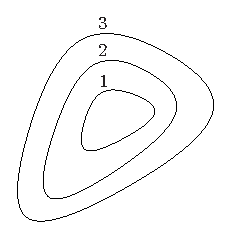
\includegraphics[width=.28\textwidth]{figures/ch03-ex127a.pdf}\end{center}
$f$ 是否可能凸、凹、拟凸或拟凹？说明理由。对下面的等高线重复上述问题。
\begin{center}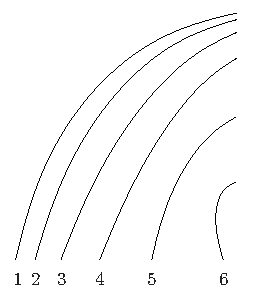
\includegraphics[width=.28\textwidth]{figures/ch03-ex127b.pdf}\end{center}
% Source PDF page 128 (printed p. 114)
\paragraph{3.3}\textit{递增凸函数的反函数。}设 $f:\R\to\R$ 在定义域 $(a,b)$ 上递增且凸。用 $g$ 表示它的反函数，即定义域为 $(f(a),f(b))$ 且对 $a<x<b$ 满足 $g(f(x))=x$ 的函数。关于 $g$ 的凸性或凹性，可以得到什么结论？
\paragraph{3.4}[RV73，第15页] 证明，连续函数 $f:\R^n\to\R$ 凸，当且仅当它在每条线段上的平均值不超过两个端点函数值的平均值：对任意 $x,y\in\R^n$，
\[\int_0^1 f(x+\lambda(y-x))\,d\lambda\leq\frac{f(x)+f(y)}2.\]
\paragraph{3.5}[RV73，第22页] \textit{凸函数的累积平均。}设 $f:\R\to\R$ 凸，$\R_+\subseteq\dom f$。证明，它的累积平均
\[F(x)=\frac1x\int_0^x f(t)\,dt,\qquad\dom F=\R_{++}\]
凸。\textit{提示：}对每个 $s$，$f(sx)$ 关于 $x$ 凸，因此 $\int_0^1 f(sx)\,ds$ 凸。
\paragraph{3.6}\textit{函数与上图。}函数的上图何时为半空间？何时为凸锥？何时为多面体？
\paragraph{3.7}设 $f:\R^n\to\R$ 凸，$\dom f=\R^n$，且在 $\R^n$ 上有上界。证明 $f$ 为常数。
\paragraph{3.8}\textit{凸性的二阶条件。}证明，二次可微函数 $f$ 凸，当且仅当其定义域凸，且对所有 $x\in\dom f$ 有 $\nabla^2f(x)\succeq0$。\textit{提示：}先考虑 $f:\R\to\R$。可以使用凸性的一阶条件，其证明见原书第70页。
\paragraph{3.9}\textit{仿射集上凸性的二阶条件。}设 $F\in\R^{n\times m}$、$\widehat x\in\R^n$。$f:\R^n\to\R$ 在仿射集 $\{Fz+\widehat x\mid z\in\R^m\}$ 上的限制定义为 $\widetilde f:\R^m\to\R$，其中
\[\widetilde f(z)=f(Fz+\widehat x),\qquad\dom\widetilde f=\{z\mid Fz+\widehat x\in\dom f\}.\]
设 $f$ 二次可微，且定义域凸。
\begin{enumerate}[label=(\alph*)]
\item 证明，$\widetilde f$ 凸，当且仅当对所有 $z\in\dom\widetilde f$ 有
\[F^\T\nabla^2f(Fz+\widehat x)F\succeq0.\]
\item 设 $A\in\R^{p\times n}$ 的零空间等于 $F$ 的值域，即 $AF=0$ 且 $\rank A=n-\rank F$。证明，若对所有 $z\in\dom\widetilde f$，存在 $\lambda\in\R$ 使
\[\nabla^2f(Fz+\widehat x)+\lambda A^\T A\succeq0,\]
则 $\widetilde f$ 凸。

\textit{提示：}使用如下结论：若 $B\in\mathbb S^n$、$A\in\R^{p\times n}$，并存在 $\lambda$ 使 $B+\lambda A^\T A\succeq0$，则对所有 $x\in\mathcal N(A)$ 有 $x^\T Bx\geq0$。
\end{enumerate}
\paragraph{3.10}\textit{Jensen 不等式的推广。}Jensen 不等式的一种解释是随机化或抖动会带来损失，即提高凸函数值的平均值：若 $f$ 凸、$v$ 为零均值随机变量，则 $\E f(x_0+v)\geq f(x_0)$。这引出如下猜想：若 $f$ 凸，则 $v$ 的方差越大，$\E f(x_0+v)$ 越大。
\begin{enumerate}[label=(\alph*)]
\item 给出反例说明这一猜想不成立。找出零均值随机变量 $v,w$，满足 $\operatorname{var}(v)>\operatorname{var}(w)$，以及凸函数 $f$ 和点 $x_0$，使 $\E f(x_0+v)<\E f(x_0+w)$。
% Source PDF page 129 (printed p. 115)
\item 当 $v,w$ 互为缩放时，这个猜想成立。证明，若 $f$ 凸且 $v$ 零均值，则 $\E f(x_0+tv)$ 在 $t\geq0$ 上单调增加。
\end{enumerate}
\paragraph{3.11}\textit{单调映射。}若函数 $\psi:\R^n\to\R^n$ 对所有 $x,y\in\dom\psi$ 满足
\[(\psi(x)-\psi(y))^\T(x-y)\geq0,\]
则称它单调。（这里“单调”的定义不同于3.6.1节，两种定义都广泛使用。）设 $f:\R^n\to\R$ 为可微凸函数。证明其梯度 $\nabla f$ 单调。逆命题是否成立，即每个单调映射都是某个凸函数的梯度吗？
\paragraph{3.12}设 $f:\R^n\to\R$ 凸、$g:\R^n\to\R$ 凹，$\dom f=\dom g=\R^n$，且对所有 $x$ 有 $g(x)\leq f(x)$。证明，存在仿射函数 $h$，对所有 $x$ 有 $g(x)\leq h(x)\leq f(x)$。换句话说，若凹函数 $g$ 是凸函数 $f$ 的下估计，则能在两者之间放入一个仿射函数。
\paragraph{3.13}\textit{Kullback--Leibler 散度与信息不等式。}设 $D_{\mathrm{kl}}$ 为式(3.17)定义的 Kullback--Leibler 散度。证明信息不等式：对所有 $u,v\in\R_{++}^n$ 有 $D_{\mathrm{kl}}(u,v)\geq0$。并证明 $D_{\mathrm{kl}}(u,v)=0$ 当且仅当 $u=v$。

\textit{提示：}Kullback--Leibler 散度可以表示为
\[D_{\mathrm{kl}}(u,v)=f(u)-f(v)-\nabla f(v)^\T(u-v),\]
其中 $f(v)=\sum_{i=1}^n v_i\log v_i$ 为 $v$ 的负熵。
\paragraph{3.14}\textit{凸—凹函数与鞍点。}若对每个固定的 $x$，$f(x,z)$ 关于 $z$ 凹，且对每个固定的 $z$，$f(x,z)$ 关于 $x$ 凸，则称 $f:\R^n\times\R^m\to\R$ 为凸—凹函数。还要求其定义域具有乘积形式 $\dom f=A\times B$，其中 $A\subseteq\R^n$、$B\subseteq\R^m$ 均凸。
\begin{enumerate}[label=(\alph*)]
\item 用 Hessian $\nabla^2f(x,z)$ 给出二次可微函数 $f:\R^n\times\R^m\to\R$ 为凸—凹函数的二阶条件。
\item 设 $f:\R^n\times\R^m\to\R$ 凸—凹且可微，$\nabla f(\widetilde x,\widetilde z)=0$。证明鞍点性质：对所有 $x,z$ 有
\[f(\widetilde x,z)\leq f(\widetilde x,\widetilde z)\leq f(x,\widetilde z).\]
证明这蕴含 $f$ 满足强极大极小性质：
\[\sup_z\inf_x f(x,z)=\inf_x\sup_z f(x,z),\]
两者的共同值为 $f(\widetilde x,\widetilde z)$。
\item 现在设 $f:\R^n\times\R^m\to\R$ 可微，但不必凸—凹，并在 $\widetilde x,\widetilde z$ 处具有鞍点性质：
\[f(\widetilde x,z)\leq f(\widetilde x,\widetilde z)\leq f(x,\widetilde z)\qquad\text{对所有 }x,z.\]
证明 $\nabla f(\widetilde x,\widetilde z)=0$。
\end{enumerate}
\subsection*{例子}
\paragraph{3.15}\textit{一族凹效用函数。}对 $0<\alpha\leq1$，令
\[u_\alpha(x)=\frac{x^\alpha-1}{\alpha},\qquad\dom u_\alpha=\R_+.\]
另定义 $u_0(x)=\log x$，$\dom u_0=\R_{++}$。
\begin{enumerate}[label=(\alph*)]
\item 证明，对 $x>0$，$u_0(x)=\lim_{\alpha\to0}u_\alpha(x)$。
% Source PDF page 130 (printed p. 116)
\item 证明各 $u_\alpha$ 凹、单调增加，并且都满足 $u_\alpha(1)=0$。
\end{enumerate}
这些函数常用于经济学，描述某种数量的商品或金钱所带来的收益或效用。$u_\alpha$ 的凹性意味着边际效用，即商品增加固定数量所获得的效用增量，随商品数量增加而减少。换句话说，凹性描述了饱和效应。
\paragraph{3.16}判断下列各函数是否凸、凹、拟凸或拟凹。
\begin{enumerate}[label=(\alph*)]
\item $\R$ 上的 $f(x)=e^x-1$。
\item $\R_{++}^2$ 上的 $f(x_1,x_2)=x_1x_2$。
\item $\R_{++}^2$ 上的 $f(x_1,x_2)=1/(x_1x_2)$。
\item $\R_{++}^2$ 上的 $f(x_1,x_2)=x_1/x_2$。
\item $\R\times\R_{++}$ 上的 $f(x_1,x_2)=x_1^2/x_2$。
\item $\R_{++}^2$ 上的 $f(x_1,x_2)=x_1^\alpha x_2^{1-\alpha}$，其中 $0\leq\alpha\leq1$。
\end{enumerate}
\paragraph{3.17}设 $p<1$、$p\ne0$。证明，函数
\[f(x)=\left(\sum_{i=1}^n x_i^p\right)^{1/p},\qquad\dom f=\R_{++}^n\]
凹。这包括特例 $f(x)=(\sum_{i=1}^n x_i^{1/2})^2$ 以及调和平均 $f(x)=(\sum_{i=1}^n1/x_i)^{-1}$。
\textit{提示：}改写3.1.5节中指数和对数函数及几何平均的证明。
\paragraph{3.18}改写3.1.5节中行列式对数函数凹性的证明，得到以下结论。
\begin{enumerate}[label=(\alph*)]
\item $f(X)=\tr(X^{-1})$ 在 $\dom f=\mathbb S_{++}^n$ 上凸。
\item $f(X)=(\det X)^{1/n}$ 在 $\dom f=\mathbb S_{++}^n$ 上凹。
\end{enumerate}
\paragraph{3.19}\textit{非负加权和与积分。}
\begin{enumerate}[label=(\alph*)]
\item 证明，$f(x)=\sum_{i=1}^r\alpha_i x_{[i]}$ 是 $x$ 的凸函数，其中 $\alpha_1\geq\alpha_2\geq\cdots\geq\alpha_r\geq0$，$x_{[i]}$ 是 $x$ 的第 $i$ 大分量。可以使用 $f(x)=\sum_{i=1}^k x_{[i]}$ 在 $\R^n$ 上凸这一事实。
\item 设 $T(x,\omega)$ 为三角多项式
\[T(x,\omega)=x_1+x_2\cos\omega+x_3\cos2\omega+\cdots+x_n\cos(n-1)\omega.\]
证明函数
\[f(x)=-\int_0^{2\pi}\log T(x,\omega)\,d\omega\]
在 $\{x\in\R^n\mid T(x,\omega)>0,\ 0\leq\omega\leq2\pi\}$ 上凸。
\end{enumerate}
\paragraph{3.20}\textit{与仿射函数复合。}证明以下函数 $f:\R^n\to\R$ 凸。
\begin{enumerate}[label=(\alph*)]
\item $f(x)=\norm{Ax-b}$，其中 $A\in\R^{m\times n}$、$b\in\R^m$，$\norm{\cdot}$ 为 $\R^m$ 上的范数。
\item $f(x)=-(\det(A_0+x_1A_1+\cdots+x_nA_n))^{1/m}$，定义域为 $\{x\mid A_0+x_1A_1+\cdots+x_nA_n\succ0\}$，其中 $A_i\in\mathbb S^m$。
\item $f(X)=\tr(A_0+x_1A_1+\cdots+x_nA_n)^{-1}$，定义域为 $\{x\mid A_0+x_1A_1+\cdots+x_nA_n\succ0\}$，其中 $A_i\in\mathbb S^m$。使用 $\tr(X^{-1})$ 在 $\mathbb S_{++}^m$ 上凸的结论，见习题3.18。
\end{enumerate}
% Source PDF page 131 (printed p. 117)
\paragraph{3.21}\textit{逐点最大值与上确界。}证明下列函数 $f:\R^n\to\R$ 凸。
\begin{enumerate}[label=(\alph*)]
\item $f(x)=\max_{i=1,\ldots,k}\norm{A^{(i)}x-b^{(i)}}$，其中 $A^{(i)}\in\R^{m\times n}$、$b^{(i)}\in\R^m$，$\norm{\cdot}$ 为 $\R^m$ 上的范数。
\item $f(x)=\sum_{i=1}^r|x|_{[i]}$，定义在 $\R^n$ 上，其中 $|x|$ 为满足 $|x|_i=|x_i|$ 的向量，即对 $x$ 逐分量取绝对值，$|x|_{[i]}$ 为 $|x|$ 的第 $i$ 大分量。换句话说，$|x|_{[1]},|x|_{[2]},\ldots,|x|_{[n]}$ 是 $x$ 的各分量绝对值按非增顺序排列后的结果。
\end{enumerate}
\paragraph{3.22}\textit{复合规则。}证明以下函数凸。
\begin{enumerate}[label=(\alph*)]
\item $f(x)=-\log(-\log(\sum_{i=1}^m e^{a_i^\T x+b_i}))$，$\dom f=\{x\mid\sum_{i=1}^m e^{a_i^\T x+b_i}<1\}$。可以使用 $\log(\sum_{i=1}^n e^{y_i})$ 凸的结论。
\item $f(x,u,v)=-\sqrt{uv-x^\T x}$，$\dom f=\{(x,u,v)\mid uv>x^\T x,\ u,v>0\}$。使用 $x^\T x/u$ 在 $u>0$ 时关于 $(x,u)$ 凸，以及 $-\sqrt{x_1x_2}$ 在 $\R_{++}^2$ 上凸这两个结论。
\item $f(x,u,v)=-\log(uv-x^\T x)$，$\dom f=\{(x,u,v)\mid uv>x^\T x,\ u,v>0\}$。
\item $f(x,t)=-(t^p-\norm x_p^p)^{1/p}$，其中 $p>1$，$\dom f=\{(x,t)\mid t\geq\norm x_p\}$。可以使用 $\norm x_p^p/u^{p-1}$ 在 $u>0$ 时关于 $(x,u)$ 凸（见习题3.23），以及 $-x^{1/p}y^{1-1/p}$ 在 $\R_+^2$ 上凸（见习题3.16）的结论。
\item $f(x,t)=-\log(t^p-\norm x_p^p)$，其中 $p>1$，$\dom f=\{(x,t)\mid t>\norm x_p\}$。可以使用 $\norm x_p^p/u^{p-1}$ 在 $u>0$ 时关于 $(x,u)$ 凸的结论，见习题3.23。
\end{enumerate}
\paragraph{3.23}\textit{函数的透视。}
\begin{enumerate}[label=(\alph*)]
\item 证明，当 $p>1$ 时，
\[f(x,t)=\frac{|x_1|^p+\cdots+|x_n|^p}{t^{p-1}}=\frac{\norm x_p^p}{t^{p-1}}\]
在 $\{(x,t)\mid t>0\}$ 上凸。
\item 证明
\[f(x)=\frac{\norm{Ax+b}_2^2}{c^\T x+d}\]
在 $\{x\mid c^\T x+d>0\}$ 上凸，其中 $A\in\R^{m\times n}$、$b\in\R^m$、$c\in\R^n$、$d\in\R$。
\end{enumerate}
\paragraph{3.24}\textit{概率单纯形上的一些函数。}设实值随机变量 $x$ 取值于 $\{a_1,\ldots,a_n\}$，其中 $a_1<a_2<\cdots<a_n$，且 $\Prob(x=a_i)=p_i$，$i=1,\ldots,n$。对下列各个关于 $p$ 的函数，在概率单纯形 $\{p\in\R_+^n\mid\one^\T p=1\}$ 上判断它是否凸、凹、拟凸或拟凹。
\begin{enumerate}[label=(\alph*)]
\item $\E x$。
\item $\Prob(x\geq\alpha)$。
\item $\Prob(\alpha\leq x\leq\beta)$。
\item $\sum_{i=1}^n p_i\log p_i$，即分布的负熵。
\item $\operatorname{var}x=\E(x-\E x)^2$。
\item $\operatorname{quartile}(x)=\inf\{\beta\mid\Prob(x\leq\beta)\geq0.25\}$。
\item 概率至少为90\% 的最小集合 $A\subseteq\{a_1,\ldots,a_n\}$ 的基数。基数指 $A$ 中元素的个数。
\item 包含90\% 概率的最窄区间的宽度，即
\[\inf\{\beta-\alpha\mid\Prob(\alpha\leq x\leq\beta)\geq0.9\}.\]
\end{enumerate}
% Source PDF page 132 (printed p. 118)
\paragraph{3.25}\textit{分布之间的最大概率距离。}设 $p,q\in\R^n$ 表示 $\{1,\ldots,n\}$ 上的两个概率分布，即 $p,q\succeq0$、$\one^\T p=\one^\T q=1$。将它们之间的最大概率距离 $d_{\mathrm{mp}}(p,q)$ 定义为所有事件上 $p,q$ 所赋概率之差的绝对值的最大值：
\[d_{\mathrm{mp}}(p,q)=\max\{|\Prob(p,C)-\Prob(q,C)|\mid C\subseteq\{1,\ldots,n\}\}.\]
这里 $\Prob(p,C)$ 为分布 $p$ 下 $C$ 的概率，即 $\Prob(p,C)=\sum_{i\in C}p_i$。

求出 $d_{\mathrm{mp}}$ 的一个简单表达式，用 $\norm{p-q}_1=\sum_{i=1}^n|p_i-q_i|$ 表示，并证明 $d_{\mathrm{mp}}$ 是 $\R^n\times\R^n$ 上的凸函数。它的定义域为 $\{(p,q)\mid p,q\succeq0,\ \one^\T p=\one^\T q=1\}$，但可以自然地延拓到整个 $\R^n\times\R^n$。
\paragraph{3.26}\textit{更多特征值函数。}设 $\lambda_1(X)\geq\lambda_2(X)\geq\cdots\geq\lambda_n(X)$ 为矩阵 $X\in\mathbb S^n$ 的特征值。前面已经看到几个关于 $X$ 凸或凹的特征值函数。
\begin{itemize}
\item 最大特征值 $\lambda_1(X)$ 凸（例3.10）；最小特征值 $\lambda_n(X)$ 凹。
\item 特征值之和，即迹 $\tr X=\lambda_1(X)+\cdots+\lambda_n(X)$，线性。
\item 特征值倒数之和，即逆矩阵的迹 $\tr(X^{-1})=\sum_{i=1}^n1/\lambda_i(X)$，在 $\mathbb S_{++}^n$ 上凸（习题3.18）。
\item 特征值的几何平均 $(\det X)^{1/n}=(\prod_{i=1}^n\lambda_i(X))^{1/n}$，以及特征值乘积的对数 $\log\det X=\sum_{i=1}^n\log\lambda_i(X)$，在 $X\in\mathbb S_{++}^n$ 上凹（习题3.18及原书第74页）。
\end{itemize}
本题利用变分刻画研究更多的特征值函数。
\begin{enumerate}[label=(\alph*)]
\item \textit{最大的 $k$ 个特征值之和。}证明 $\sum_{i=1}^k\lambda_i(X)$ 在 $\mathbb S^n$ 上凸。
\textit{提示：}[HJ85，第191页] 使用变分刻画
\[\sum_{i=1}^k\lambda_i(X)=\sup\{\tr(V^\T XV)\mid V\in\R^{n\times k},\ V^\T V=I\}.\]
\item \textit{最小的 $k$ 个特征值的几何平均。}证明 $(\prod_{i=n-k+1}^n\lambda_i(X))^{1/k}$ 在 $\mathbb S_{++}^n$ 上凹。
\textit{提示：}[MO79，第513页] 对 $X\succ0$，
\[\left(\prod_{i=n-k+1}^n\lambda_i(X)\right)^{1/k}
 =\frac1k\inf\{\tr(V^\T XV)\mid V\in\R^{n\times k},\ \det V^\T V=1\}.\]
\item \textit{最小的 $k$ 个特征值乘积的对数。}证明 $\sum_{i=n-k+1}^n\log\lambda_i(X)$ 在 $\mathbb S_{++}^n$ 上凹。
\textit{提示：}[MO79，第513页] 对 $X\succ0$，
\[\prod_{i=n-k+1}^n\lambda_i(X)
 =\inf\left\{\prod_{i=1}^k(V^\T XV)_{ii}\ \middle|\ V\in\R^{n\times k},\ V^\T V=I\right\}.\]
\end{enumerate}
\paragraph{3.27}\textit{Cholesky 因子的对角元。}每个 $X\in\mathbb S_{++}^n$ 都有唯一 Cholesky 分解 $X=LL^\T$，其中 $L$ 为下三角矩阵且 $L_{ii}>0$。证明 $L_{ii}$ 是 $X$ 的凹函数，定义域为 $\mathbb S_{++}^n$。

\textit{提示：}$L_{ii}$ 可表示为 $L_{ii}=(w-z^\T Y^{-1}z)^{1/2}$，其中
\[\begin{bmatrix}Y&z\\z^\T&w\end{bmatrix}\]
是 $X$ 的前 $i\times i$ 主子矩阵。
% Source PDF page 133 (printed p. 119)
\subsection*{保持凸性的运算}
\paragraph{3.28}\textit{把凸函数表示成一族仿射函数的逐点上确界。}本题将原书第83页证明的结论推广到 $\dom f\ne\R^n$。设 $f:\R^n\to\R$ 凸。定义 $\widetilde f:\R^n\to\R$ 为 $f$ 的所有仿射全局下估计的逐点上确界：
\[\widetilde f(x)=\sup\{g(x)\mid g\text{ 仿射},\ g(z)\leq f(z)\text{ 对所有 }z\text{ 成立}\}.\]
\begin{enumerate}[label=(\alph*)]
\item 证明，对 $x\in\operatorname{int}\dom f$，$f(x)=\widetilde f(x)$。
\item 证明，若 $f$ 闭，即 $\epi f$ 为闭集（见A.3.3节），则 $f=\widetilde f$。
\end{enumerate}
\paragraph{3.29}\textit{分段线性凸函数的表示。}凸函数 $f:\R^n\to\R$、$\dom f=\R^n$，若存在 $\R^n$ 的划分
\[\R^n=X_1\cup X_2\cup\cdots\cup X_L,\]
其中 $\operatorname{int}X_i\ne\varnothing$，且 $i\ne j$ 时 $\operatorname{int}X_i\cap\operatorname{int}X_j=\varnothing$，并有一族仿射函数 $a_1^\T x+b_1,\ldots,a_L^\T x+b_L$，使得 $x\in X_i$ 时 $f(x)=a_i^\T x+b_i$，则称 $f$ 分段线性。

证明，此类函数具有形式 $f(x)=\max\{a_1^\T x+b_1,\ldots,a_L^\T x+b_L\}$。
\paragraph{3.30}\textit{函数的凸包或凸包络。}函数 $f:\R^n\to\R$ 的凸包或凸包络定义为
\[g(x)=\inf\{t\mid(x,t)\in\conv\epi f\}.\]
几何上，$g$ 的上图是 $f$ 上图的凸包。

证明，$g$ 是 $f$ 的最大凸下估计。也就是说，若 $h$ 凸且对所有 $x$ 有 $h(x)\leq f(x)$，则对所有 $x$ 都有 $h(x)\leq g(x)$。
\paragraph{3.31}[Roc70，第35页] \textit{最大的齐次下估计。}设 $f$ 为凸函数，定义
\[g(x)=\inf_{\alpha>0}\frac{f(\alpha x)}\alpha.\]
\begin{enumerate}[label=(\alph*)]
\item 证明 $g$ 齐次，即对所有 $t\geq0$ 有 $g(tx)=tg(x)$。
\item 证明 $g$ 为 $f$ 的最大齐次下估计：若 $h$ 齐次且对所有 $x$ 有 $h(x)\leq f(x)$，则对所有 $x$ 有 $h(x)\leq g(x)$。
\item 证明 $g$ 凸。
\end{enumerate}
\paragraph{3.32}\textit{凸函数的乘积与比值。}一般来说，两个凸函数的乘积或比值不凸。但对 $\R$ 上函数存在一些结论。证明以下命题。
\begin{enumerate}[label=(\alph*)]
\item 若 $f,g$ 是区间上的正凸函数，并且都单调不减或都单调不增，则 $fg$ 凸。
\item 若 $f,g$ 为正凹函数，其中一个单调不减，另一个单调不增，则 $fg$ 凹。
\item 若 $f$ 凸、单调不减且为正，$g$ 凹、单调不增且为正，则 $f/g$ 凸。
\end{enumerate}
\paragraph{3.33}\textit{透视定理的直接证明。}直接证明：按3.2.6节定义的凸函数 $f$ 的透视 $g$ 凸。证明 $\dom g$ 为凸集，且对 $(x,t),(y,s)\in\dom g$、$0\leq\theta\leq1$ 有
\[g(\theta x+(1-\theta)y,\theta t+(1-\theta)s)\leq\theta g(x,t)+(1-\theta)g(y,s).\]
\paragraph{3.34}\textit{Minkowski 函数。}凸集 $C$ 的 Minkowski 函数定义为
\[M_C(x)=\inf\{t>0\mid t^{-1}x\in C\}.\]
% Source PDF page 134 (printed p. 120)
\begin{enumerate}[label=(\alph*)]
\item 画图，从几何上说明怎样求 $M_C(x)$。
\item 证明 $M_C$ 齐次，即对 $\alpha\geq0$ 有 $M_C(\alpha x)=\alpha M_C(x)$。
\item $\dom M_C$ 是什么？
\item 证明 $M_C$ 为凸函数。
\item 再设 $C$ 闭、有界、对称（$x\in C$ 蕴含 $-x\in C$），并有非空内部。证明 $M_C$ 为范数。对应的单位球是什么？
\end{enumerate}
\paragraph{3.35}\textit{支撑函数运算。}回顾，集合 $C\subseteq\R^n$ 的支撑函数定义为 $S_C(y)=\sup\{y^\T x\mid x\in C\}$。原书第81页已证明 $S_C$ 凸。
\begin{enumerate}[label=(\alph*)]
\item 证明 $S_B=S_{\conv B}$。
\item 证明 $S_{A+B}=S_A+S_B$。
\item 证明 $S_{A\cup B}=\max\{S_A,S_B\}$。
\item 设 $B$ 闭且凸。证明，$A\subseteq B$ 当且仅当对所有 $y$ 有 $S_A(y)\leq S_B(y)$。
\end{enumerate}
\subsection*{共轭函数}
\paragraph{3.36}求下列函数的共轭。
\begin{enumerate}[label=(\alph*)]
\item \textit{最大值函数。}$\R^n$ 上的 $f(x)=\max_{i=1,\ldots,n}x_i$。
\item \textit{最大元素之和。}$\R^n$ 上的 $f(x)=\sum_{i=1}^r x_{[i]}$。
\item \textit{$\R$ 上的分段线性函数。}$\R$ 上的 $f(x)=\max_{i=1,\ldots,m}(a_ix+b_i)$。可以假设 $a_i$ 已按递增顺序排列，即 $a_1\leq\cdots\leq a_m$，且每个函数 $a_ix+b_i$ 都不冗余，即对每个 $k$ 至少存在一个 $x$ 使 $f(x)=a_kx+b_k$。
\item \textit{幂函数。}$\R_{++}$ 上的 $f(x)=x^p$，$p>1$。再对 $p<0$ 求解。
\item \textit{负几何平均。}$\R_{++}^n$ 上的 $f(x)=-(\prod x_i)^{1/n}$。
\item \textit{二阶锥的负广义对数。}$f(x,t)=-\log(t^2-x^\T x)$，定义在 $\{(x,t)\in\R^n\times\R\mid\norm x_2<t\}$ 上。
\end{enumerate}
\paragraph{3.37}证明，$f(X)=\tr(X^{-1})$、$\dom f=\mathbb S_{++}^n$ 的共轭为
\[f^*(Y)=-2\tr(-Y)^{1/2},\qquad\dom f^*=-\mathbb S_+^n.\]
\textit{提示：}$f$ 的梯度为 $\nabla f(X)=-X^{-2}$。
\paragraph{3.38}\textit{Young 不等式。}设 $f:\R\to\R$ 为递增函数，$f(0)=0$，其反函数为 $g$。定义 $F,G$ 为
\[F(x)=\int_0^x f(a)\,da,\qquad G(y)=\int_0^y g(a)\,da.\]
证明 $F,G$ 互为共轭。给出 Young 不等式
\[xy\leq F(x)+G(y)\]
的简单几何解释。
\paragraph{3.39}\textit{共轭函数的性质。}
\begin{enumerate}[label=(\alph*)]
\item \textit{凸函数加仿射函数的共轭。}定义 $g(x)=f(x)+c^\T x+d$，其中 $f$ 凸。用 $f^*$ 及 $c,d$ 表示 $g^*$。
\item \textit{透视的共轭。}用凸函数 $f$ 的共轭 $f^*$ 表示其透视的共轭。
% Source PDF page 135 (printed p. 121)
\item \textit{共轭与最小化。}设 $f(x,z)$ 关于 $(x,z)$ 凸，定义 $g(x)=\inf_z f(x,z)$。用 $f^*$ 表示共轭 $g^*$。

作为应用，设 $h$ 凸，用 $h^*,A,b$ 表示 $g(x)=\inf_z\{h(z)\mid Az+b=x\}$ 的共轭。
\item \textit{共轭的共轭。}证明，闭凸函数的共轭的共轭是其本身：若 $f$ 闭且凸，则 $f=f^{**}$。函数闭指其上图闭，见A.3.3节。
\textit{提示：}证明 $f^{**}$ 是 $f$ 的所有仿射全局下估计的逐点上确界，再应用习题3.28。
\end{enumerate}
\paragraph{3.40}\textit{共轭函数的梯度与 Hessian。}设 $f:\R^n\to\R$ 凸、二次连续可微。设 $\bar y$ 与 $\bar x$ 满足 $\bar y=\nabla f(\bar x)$，且 $\nabla^2f(\bar x)\succ0$。
\begin{enumerate}[label=(\alph*)]
\item 证明 $\nabla f^*(\bar y)=\bar x$。
\item 证明 $\nabla^2f^*(\bar y)=\nabla^2f(\bar x)^{-1}$。
\end{enumerate}
\paragraph{3.41}\textit{负归一化熵的共轭。}证明，负归一化熵
\[f(x)=\sum_{i=1}^n x_i\log(x_i/\one^\T x),\qquad\dom f=\R_{++}^n\]
的共轭为
\[f^*(y)=\begin{cases}0,&\sum_{i=1}^n e^{y_i}\leq1,\\+\infty,&\text{其他情况}.\end{cases}\]
\subsection*{拟凸函数}
\paragraph{3.42}\textit{近似宽度。}设给定连续函数 $f_0,\ldots,f_n:\R\to\R$。考虑用 $f_1,\ldots,f_n$ 的线性组合近似 $f_0$。对于 $x\in\R^n$，若对 $0\leq t\leq T$ 有 $|f(t)-f_0(t)|\leq\epsilon$，则称 $f=x_1f_1+\cdots+x_nf_n$ 在区间 $[0,T]$ 上以容差 $\epsilon>0$ 近似 $f_0$。固定容差 $\epsilon>0$，将近似宽度定义为 $f$ 能在 $[0,T]$ 上近似 $f_0$ 的最大 $T$：
\[W(x)=\sup\{T\mid |x_1f_1(t)+\cdots+x_nf_n(t)-f_0(t)|\leq\epsilon,\ 0\leq t\leq T\}.\]
证明 $W$ 拟凹。
\paragraph{3.43}\textit{拟凸性的一阶条件。}证明3.4.3节的拟凸性一阶条件：具有凸定义域的可微函数 $f:\R^n\to\R$ 拟凸，当且仅当对所有 $x,y\in\dom f$ 有
\[f(y)\leq f(x)\ \Longrightarrow\ \nabla f(x)^\T(y-x)\leq0.\]
\textit{提示：}只需对 $\R$ 上的函数证明；一般情形由限制在任意直线上得到。
\paragraph{3.44}\textit{拟凸性的二阶条件。}本题导出3.4.3节拟凸性二阶条件的其他表示。证明以下结论。
\begin{enumerate}[label=(\alph*)]
\item 若存在 $\sigma$ 使
\begin{equation}\nabla^2f(x)+\sigma\nabla f(x)\nabla f(x)^\T\succeq0,\tag{3.26}\end{equation}
则点 $x\in\dom f$ 满足式(3.21)。对所有 $y\ne0$ 满足式(3.22)，当且仅当存在 $\sigma$ 使
\begin{equation}\nabla^2f(x)+\sigma\nabla f(x)\nabla f(x)^\T\succ0.\tag{3.27}\end{equation}
\textit{提示：}可不失一般性地假设 $\nabla^2f(x)$ 为对角矩阵。
% Source PDF page 136 (printed p. 122)
\item 点 $x\in\dom f$ 满足式(3.21)，当且仅当或者 $\nabla f(x)=0$ 且 $\nabla^2f(x)\succeq0$，或者 $\nabla f(x)\ne0$ 且矩阵
\[H(x)=\begin{bmatrix}\nabla^2f(x)&\nabla f(x)\\\nabla f(x)^\T&0\end{bmatrix}\]
恰有一个负特征值。它对所有 $y\ne0$ 满足式(3.22)，当且仅当 $H(x)$ 恰有一个非正特征值。

\textit{提示：}可以使用(a)的结论。以下结论由线性代数中的特征值交错定理推出，也可能有用：若 $B\in\mathbb S^n$、$a\in\R^n$，则
\[\lambda_n\left(\begin{bmatrix}B&a\\a^\T&0\end{bmatrix}\right)\geq\lambda_n(B).\]
\end{enumerate}
\paragraph{3.45}利用3.4.3节给出的拟凸性一阶、二阶条件，验证函数 $f(x)=-x_1x_2$、$\dom f=\R_{++}^2$ 拟凸。
\paragraph{3.46}\textit{定义域为 $\R^n$ 的拟线性函数。}$\R$ 上的拟线性函数，即既拟凸又拟凹的函数，单调，也就是单调不减或单调不增。本题考虑这一结论向 $\R^n$ 上函数的推广。

设 $f:\R^n\to\R$ 拟线性且连续，$\dom f=\R^n$。证明，可以将它表示为 $f(x)=g(a^\T x)$，其中 $g:\R\to\R$ 单调、$a\in\R^n$。换句话说，定义域为 $\R^n$ 的拟线性函数，必为某个线性函数的单调函数。逆命题也成立。
\subsection*{对数凹函数与对数凸函数}
\paragraph{3.47}设 $f:\R^n\to\R$ 可微，$\dom f$ 凸，并对所有 $x\in\dom f$ 有 $f(x)>0$。证明，$f$ 对数凹，当且仅当对所有 $x,y\in\dom f$ 有
\[\frac{f(y)}{f(x)}\leq\exp\left(\frac{\nabla f(x)^\T(y-x)}{f(x)}\right).\]
\paragraph{3.48}证明，若 $f:\R^n\to\R$ 对数凹、$a\geq0$，则函数 $g=f-a$ 对数凹，其中 $\dom g=\{x\in\dom f\mid f(x)>a\}$。
\paragraph{3.49}证明下列函数对数凹。
\begin{enumerate}[label=(\alph*)]
\item Logistic 函数：$f(x)=e^x/(1+e^x)$，$\dom f=\R$。
\item 调和平均：
\[f(x)=\frac1{1/x_1+\cdots+1/x_n},\qquad\dom f=\R_{++}^n.\]
\item 乘积除以和：
\[f(x)=\frac{\prod_{i=1}^n x_i}{\sum_{i=1}^n x_i},\qquad\dom f=\R_{++}^n.\]
\item 行列式除以迹：
\[f(X)=\frac{\det X}{\tr X},\qquad\dom f=\mathbb S_{++}^n.\]
\end{enumerate}
% Source PDF page 137 (printed p. 123)
\paragraph{3.50}\textit{多项式系数作为根的函数。}证明，具有负实根的多项式的系数，是根的对数凹函数。换句话说，由恒等式
\[s^n+a_1(\lambda)s^{n-1}+\cdots+a_{n-1}(\lambda)s+a_n(\lambda)
 =(s-\lambda_1)(s-\lambda_2)\cdots(s-\lambda_n)\]
定义的函数 $a_i:\R^n\to\R$，在 $-\R_{++}^n$ 上对数凹。

\textit{提示：}函数
\[S_k(x)=\sum_{1\leq i_1<i_2<\cdots<i_k\leq n}x_{i_1}x_{i_2}\cdots x_{i_k},\]
定义域为 $\R_+^n$，$1\leq k\leq n$，称为 $\R^n$ 上的第 $k$ 个初等对称函数。可以证明 $S_k^{1/k}$ 凹，见 [ML57]。
\paragraph{3.51}[BL00，第41页] 设 $p$ 是 $\R$ 上的多项式，所有根都为实数。证明，在它取正值的任意区间上，它对数凹。
\paragraph{3.52}[MO79，第3.E.2节] \textit{矩函数的对数凸性。}设 $f:\R\to\R$ 非负，$\R_+\subseteq\dom f$。对 $x\geq0$，定义
\[\phi(x)=\int_0^\infty u^xf(u)\,du.\]
证明 $\phi$ 对数凸。若 $x$ 为正整数、$f$ 为概率密度函数，则 $\phi(x)$ 为分布的第 $x$ 阶矩。

利用这一结论证明 Gamma 函数
\[\Gamma(x)=\int_0^\infty u^{x-1}e^{-u}\,du\]
在 $x\geq1$ 时对数凸。
\paragraph{3.53}设 $x,y$ 为 $\R^n$ 中独立随机向量，分别具有对数凹概率密度 $f,g$。证明，和 $z=x+y$ 的概率密度对数凹。
\paragraph{3.54}\textit{高斯累积分布函数的对数凹性。}高斯随机变量的累积分布函数
\[f(x)=\frac1{\sqrt{2\pi}}\int_{-\infty}^x e^{-t^2/2}\,dt\]
对数凹。这可以由“两个对数凹函数的卷积对数凹”这一一般结论推出。本题引导你给出一个简单、自成体系的证明。回顾，$f$ 对数凹，当且仅当对所有 $x$ 有 $f''(x)f(x)\leq f'(x)^2$。
\begin{enumerate}[label=(\alph*)]
\item 验证当 $x\geq0$ 时，$f''(x)f(x)\leq f'(x)^2$。这样只剩下较难的 $x<0$ 部分。
\item 验证对任意 $t,x$ 都有 $t^2/2\geq-x^2/2+xt$。
\item 利用(b)证明 $e^{-t^2/2}\leq e^{x^2/2-xt}$。从而对 $x<0$，
\[\int_{-\infty}^x e^{-t^2/2}\,dt\leq e^{x^2/2}\int_{-\infty}^x e^{-xt}\,dt.\]
\item 利用(c)验证，当 $x\leq0$ 时，$f''(x)f(x)\leq f'(x)^2$。
\end{enumerate}
% Source PDF page 138 (printed p. 124)
\paragraph{3.55}\textit{对数凹概率密度的累积分布函数的对数凹性。}本题推广习题3.54的结论。设 $g(t)=\exp(-h(t))$ 是可微的对数凹概率密度函数，令
\[f(x)=\int_{-\infty}^x g(t)\,dt=\int_{-\infty}^x e^{-h(t)}\,dt\]
为其累积分布。将证明 $f$ 对数凹，即对所有 $x$ 满足 $f''(x)f(x)\leq(f'(x))^2$。
\begin{enumerate}[label=(\alph*)]
\item 用函数 $h$ 表示 $f$ 的各阶导数。验证当 $h'(x)\geq0$ 时，$f''(x)f(x)\leq(f'(x))^2$。
\item 设 $h'(x)<0$。利用由 $h$ 的凸性得到的不等式
\[h(t)\geq h(x)+h'(x)(t-x),\]
证明
\[\int_{-\infty}^x e^{-h(t)}\,dt\leq\frac{e^{-h(x)}}{-h'(x)}.\]
利用这个不等式验证，当 $h'(x)<0$ 时，$f''(x)f(x)\leq(f'(x))^2$。
\end{enumerate}
\paragraph{3.56}\textit{更多对数凹密度。}证明以下密度对数凹。
\begin{enumerate}[label=(\alph*)]
\item [MO79，第493页] Gamma 密度，定义为
\[f(x)=\frac{\alpha^\lambda}{\Gamma(\lambda)}x^{\lambda-1}e^{-\alpha x},\qquad\dom f=\R_+.\]
参数 $\lambda,\alpha$ 满足 $\lambda\geq1$、$\alpha>0$。
\item [MO79，第306页] Dirichlet 密度
\[
 f(x)=\frac{\Gamma(\one^\T\lambda)}{\Gamma(\lambda_1)\cdots\Gamma(\lambda_{n+1})}
 x_1^{\lambda_1-1}\cdots x_n^{\lambda_n-1}
 \left(1-\sum_{i=1}^n x_i\right)^{\lambda_{n+1}-1},
\]
定义域为 $\dom f=\{x\in\R_{++}^n\mid\one^\T x<1\}$，参数 $\lambda$ 满足 $\lambda\succeq\one$。
\end{enumerate}
\subsection*{相对于广义不等式的凸性}
\paragraph{3.57}证明函数 $f(X)=X^{-1}$ 在 $\mathbb S_{++}^n$ 上矩阵凸。
\paragraph{3.58}\textit{Schur 补。}设 $X\in\mathbb S^n$ 分块为
\[X=\begin{bmatrix}A&B\\B^\T&C\end{bmatrix},\]
其中 $A\in\mathbb S^k$。$X$ 关于 $A$ 的 Schur 补为 $S=C-B^\T A^{-1}B$，见A.5.5节。证明，作为从 $\mathbb S^n$ 到 $\mathbb S^{n-k}$ 的函数，Schur 补在 $\mathbb S_{++}^n$ 上矩阵凹。
\paragraph{3.59}\textit{$K$-凸性的二阶条件。}设 $K\subseteq\R^m$ 为正常凸锥，对应广义不等式 $\preceq_K$。证明，具有凸定义域的二次可微函数 $f:\R^n\to\R^m$ 为 $K$-凸函数，当且仅当对所有 $x\in\dom f$ 及所有 $y\in\R^n$，有
\[\sum_{i,j=1}^n y_iy_j\frac{\partial^2f(x)}{\partial x_i\partial x_j}\succeq_K0,\]
即二阶导数是 $K$-非负双线性型。这里 $\partial^2f/\partial x_i\partial x_j\in\R^m$，其分量为 $\partial^2f_k/\partial x_i\partial x_j$，$k=1,\ldots,m$；见A.4.1节。
% Source PDF page 139 (printed p. 125)
\paragraph{3.60}\textit{$K$-凸函数的下水平集与上图。}设 $K\subseteq\R^m$ 为正常凸锥，对应广义不等式 $\preceq_K$，$f:\R^n\to\R^m$。对 $\alpha\in\R^m$，$f$ 关于 $\preceq_K$ 的 $\alpha$-下水平集定义为
\[C_\alpha=\{x\in\R^n\mid f(x)\preceq_K\alpha\}.\]
$f$ 关于 $\preceq_K$ 的上图定义为
\[\epi_K f=\{(x,t)\in\R^{n+m}\mid f(x)\preceq_K t\}.\]
证明：
\begin{enumerate}[label=(\alph*)]
\item 若 $f$ 为 $K$-凸函数，则对所有 $\alpha$，下水平集 $C_\alpha$ 凸。
\item $f$ 为 $K$-凸函数，当且仅当 $\epi_K f$ 为凸集。
\end{enumerate}
% Source PDF page 140 (printed p. 126): blank page in source.


\chapter{凸优化问题}
% Source PDF page 141 (printed p. 127)
\section{优化问题}
\subsection{基本术语}
我们用记号
\begin{equation}
\begin{array}{ll}
\text{最小化}&f_0(x)\\
\text{约束为}&f_i(x)\le0,\quad i=1,\ldots,m,\\
&h_i(x)=0,\quad i=1,\ldots,p
\end{array}\tag{4.1}
\end{equation}
表示这样一个问题：在满足条件 $f_i(x)\le0$（$i=1,\ldots,m$）和 $h_i(x)=0$（$i=1,\ldots,p$）的所有 $x$ 中，求使 $f_0(x)$ 最小的 $x$。我们称 $x\in\R^n$ 为优化变量，称函数 $f_0:\R^n\to\R$ 为目标函数或成本函数。不等式 $f_i(x)\le0$ 称为不等式约束，对应的函数 $f_i:\R^n\to\R$ 称为不等式约束函数。等式 $h_i(x)=0$ 称为等式约束，函数 $h_i:\R^n\to\R$ 称为等式约束函数。若没有约束，即 $m=p=0$，就称问题（4.1）为无约束问题。

目标函数和全部约束函数都有定义的点构成的集合
\[
\mathcal D=\bigcap_{i=0}^m\dom f_i\ \cap\ \bigcap_{i=1}^p\dom h_i
\]
称为优化问题（4.1）的定义域。若点 $x\in\mathcal D$ 满足约束 $f_i(x)\le0$（$i=1,\ldots,m$）及 $h_i(x)=0$（$i=1,\ldots,p$），就称它为可行点。若至少存在一个可行点，就称问题（4.1）可行；否则称其不可行。全部可行点构成的集合称为可行集或约束集。

问题（4.1）的最优值 $p^\star$ 定义为
\[
p^\star=\inf\{f_0(x)\mid f_i(x)\le0,\ i=1,\ldots,m,\ h_i(x)=0,\ i=1,\ldots,p\}.
\]
我们允许 $p^\star$ 取广义值 $\pm\infty$。若问题不可行，则 $p^\star=\infty$，这里采用空集下确界为 $\infty$ 的通常约定。

% Source PDF page 142 (printed p. 128)
若存在可行点序列 $x_k$，使 $k\to\infty$ 时 $f_0(x_k)\to-\infty$，则 $p^\star=-\infty$，此时称问题（4.1）无下界。

\subsubsection*{最优点与局部最优点}
若 $x^\star$ 可行且 $f_0(x^\star)=p^\star$，我们就称 $x^\star$ 为最优点，或说它解出了问题（4.1）。全部最优点构成最优集，记为
\[
X_{\mathrm{opt}}=\{x\mid f_i(x)\le0,\ i=1,\ldots,m,\ h_i(x)=0,\ i=1,\ldots,p,\ f_0(x)=p^\star\}.
\]
若问题（4.1）存在最优点，就称最优值能够取到或达到，并称问题可解。若 $X_{\mathrm{opt}}$ 为空，则称最优值不能取到或达到。（问题无下界时总是如此。）满足 $f_0(x)\le p^\star+\epsilon$（其中 $\epsilon>0$）的可行点 $x$ 称为 $\epsilon$ 次优点，全部 $\epsilon$ 次优点构成的集合称为问题（4.1）的 $\epsilon$ 次优集。

若存在 $R>0$，使可行点 $x$ 满足
\[
f_0(x)=\inf\{f_0(z)\mid f_i(z)\le0,\ i=1,\ldots,m,\ h_i(z)=0,\ i=1,\ldots,p,\ \norm{z-x}_2\le R\},
\]
就称 $x$ 为局部最优点。换言之，$x$ 解出了以 $z$ 为变量的优化问题
\[
\begin{array}{ll}
\text{最小化}&f_0(z)\\
\text{约束为}&f_i(z)\le0,\quad i=1,\ldots,m,\\
&h_i(z)=0,\quad i=1,\ldots,p,\\
&\norm{z-x}_2\le R.
\end{array}
\]
粗略地说，这意味着 $x$ 在可行集中邻近的点上使 $f_0$ 最小。有时用“全局最优”代替“最优”，以区别于“局部最优”。不过，本书中的“最优”始终指全局最优。

若 $x$ 可行且 $f_i(x)=0$，就称第 $i$ 个不等式约束 $f_i(x)\le0$ 在 $x$ 处是活跃的。若 $f_i(x)<0$，则称该约束不活跃。（等式约束在所有可行点处都是活跃的。）若删除一个约束不改变可行集，就称它是冗余约束。

\begin{origexample}{4.1}
我们用几个简单的无约束优化问题说明上述定义，其中变量 $x\in\R$，且 $\dom f_0=\R_{++}$。
\begin{itemize}
\item $f_0(x)=1/x$：$p^\star=0$，但最优值不能达到。
\item $f_0(x)=-\log x$：$p^\star=-\infty$，所以问题无下界。
\item $f_0(x)=x\log x$：$p^\star=-1/e$，在唯一最优点 $x^\star=1/e$ 处达到。
\end{itemize}
\end{origexample}

\subsubsection*{可行性问题}
若目标函数恒为零，则最优值或者为零（可行集非空时），或者为 $\infty$（可行集为空时）。我们称其为可行性问题，有时写为

% Source PDF page 143 (printed p. 129)
\[
\begin{array}{ll}
\text{求}&x\\
\text{使得}&f_i(x)\le0,\quad i=1,\ldots,m,\\
&h_i(x)=0,\quad i=1,\ldots,p.
\end{array}
\]
因此，可行性问题就是判断约束是否相容；若相容，则求一个满足全部约束的点。

\subsection{将问题写成标准形式}
我们称（4.1）为标准形式优化问题。在标准形式中，约定不等式和等式约束的右端均为零。将非零右端移到左端，总能做到这一点。例如，把等式约束 $g_i(x)=\widetilde g_i(x)$ 写为 $h_i(x)=0$，其中 $h_i(x)=g_i(x)-\widetilde g_i(x)$。类似地，把 $f_i(x)\ge0$ 写成 $-f_i(x)\le0$。

\begin{origexample}{4.2}
\textbf{盒约束。}考虑优化问题
\[
\begin{array}{ll}
\text{最小化}&f_0(x)\\
\text{约束为}&l_i\le x_i\le u_i,\quad i=1,\ldots,n,
\end{array}
\]
其中变量为 $x\in\R^n$。这些约束称为变量界，因为它们给出每个 $x_i$ 的下界和上界；也称为盒约束，因为可行集是一个盒。

可以将此问题写成标准形式
\[
\begin{array}{ll}
\text{最小化}&f_0(x)\\
\text{约束为}&l_i-x_i\le0,\quad i=1,\ldots,n,\\
&x_i-u_i\le0,\quad i=1,\ldots,n.
\end{array}
\]
共有 $2n$ 个不等式约束函数：
\[
f_i(x)=l_i-x_i,\quad i=1,\ldots,n,
\]
以及
\[
f_i(x)=x_{i-n}-u_{i-n},\quad i=n+1,\ldots,2n.
\]
\end{origexample}

\subsubsection*{最大化问题}
按照惯例，我们主要讨论最小化问题。对于最大化问题
\begin{equation}
\begin{array}{ll}
\text{最大化}&f_0(x)\\
\text{约束为}&f_i(x)\le0,\quad i=1,\ldots,m,\\
&h_i(x)=0,\quad i=1,\ldots,p,
\end{array}\tag{4.2}
\end{equation}

% Source PDF page 144 (printed p. 130)
可在相同约束下最小化函数 $-f_0$ 来求解。利用这一对应关系，可以为最大化问题（4.2）定义上述全部术语。例如，（4.2）的最优值定义为
\[
p^\star=\sup\{f_0(x)\mid f_i(x)\le0,\ i=1,\ldots,m,\ h_i(x)=0,\ i=1,\ldots,p\},
\]
而可行点 $x$ 为 $\epsilon$ 次优点的条件为 $f_0(x)\ge p^\star-\epsilon$。讨论最大化问题时，有时将目标称为效用或满意程度，而非成本。

\subsection{等价问题}
本书以非形式化的方式使用优化问题的等价性概念。如果由一个问题的解容易得到另一个问题的解，反之亦然，就称两个问题等价。（可以严格定义等价性，但定义比较复杂。）

作为一个简单例子，考虑问题
\begin{equation}
\begin{array}{ll}
\text{最小化}&\widetilde f_0(x)=\alpha_0f_0(x)\\
\text{约束为}&\widetilde f_i(x)=\alpha_if_i(x)\le0,\quad i=1,\ldots,m,\\
&\widetilde h_i(x)=\beta_ih_i(x)=0,\quad i=1,\ldots,p,
\end{array}\tag{4.3}
\end{equation}
其中 $\alpha_i>0$（$i=0,\ldots,m$），$\beta_i\ne0$（$i=1,\ldots,p$）。此问题由标准形式问题（4.1）得到：目标函数和不等式约束函数分别乘以正数，等式约束函数分别乘以非零常数。因此，（4.3）与原问题（4.1）的可行集相同。点 $x$ 为原问题（4.1）的最优点，当且仅当它为缩放后问题（4.3）的最优点，所以我们称两个问题等价。但这两个问题并不相同（除非所有 $\alpha_i$ 和 $\beta_i$ 均为一），因为目标函数和约束函数不同。下面介绍几种产生等价问题的一般变换。

\subsubsection*{变量变换}
设 $\phi:\R^n\to\R^n$ 是一一映射，其像包含问题的定义域 $\mathcal D$，即 $\phi(\dom\phi)\supseteq\mathcal D$。定义函数 $\widetilde f_i$ 和 $\widetilde h_i$ 为
\[
\widetilde f_i(z)=f_i(\phi(z)),\quad i=0,\ldots,m,\qquad
\widetilde h_i(z)=h_i(\phi(z)),\quad i=1,\ldots,p.
\]
考虑以 $z$ 为变量的问题
\begin{equation}
\begin{array}{ll}
\text{最小化}&\widetilde f_0(z)\\
\text{约束为}&\widetilde f_i(z)\le0,\quad i=1,\ldots,m,\\
&\widetilde h_i(z)=0,\quad i=1,\ldots,p.
\end{array}\tag{4.4}
\end{equation}
我们称标准形式问题（4.1）与问题（4.4）由变量变换或变量代换 $x=\phi(z)$ 联系起来。两个问题显然等价：若 $x$ 解出问题（4.1），则 $z=\phi^{-1}(x)$ 解出问题（4.4）；若 $z$ 解出问题（4.4），则 $x=\phi(z)$ 解出问题（4.1）。

% Source PDF page 145 (printed p. 131)
\subsubsection*{目标函数和约束函数的变换}
设 $\psi_0:\R\to\R$ 单调递增，$\psi_1,\ldots,\psi_m:\R\to\R$ 满足 $\psi_i(u)\le0$ 当且仅当 $u\le0$，$\psi_{m+1},\ldots,\psi_{m+p}:\R\to\R$ 满足 $\psi_i(u)=0$ 当且仅当 $u=0$。定义复合函数
\[
\widetilde f_i(x)=\psi_i(f_i(x)),\quad i=0,\ldots,m,\qquad
\widetilde h_i(x)=\psi_{m+i}(h_i(x)),\quad i=1,\ldots,p.
\]
相应问题
\[
\begin{array}{ll}
\text{最小化}&\widetilde f_0(x)\\
\text{约束为}&\widetilde f_i(x)\le0,\quad i=1,\ldots,m,\\
&\widetilde h_i(x)=0,\quad i=1,\ldots,p
\end{array}
\]
显然与标准形式问题（4.1）等价；实际上，两者的可行集相同，最优点也相同。（前面将目标函数和约束函数乘以适当常数的例子（4.3），是所有 $\psi_i$ 均为线性函数的特殊情形。）

\begin{origexample}{4.3}
\textbf{最小范数与最小范数平方问题。}考虑以 $x\in\R^n$ 为变量的无约束欧氏范数最小化问题
\begin{equation}
\text{最小化}\quad\norm{Ax-b}_2.\tag{4.5}
\end{equation}
由于范数总是非负，也可以求解
\begin{equation}
\text{最小化}\quad\norm{Ax-b}_2^2=(Ax-b)^\T(Ax-b),\tag{4.6}
\end{equation}
即最小化欧氏范数的平方。问题（4.5）与（4.6）显然等价，最优点相同；但二者并不是同一个问题。例如，（4.5）的目标在任何满足 $Ax-b=0$ 的 $x$ 处都不可微，而（4.6）的目标对所有 $x$ 都可微（实际上是二次函数）。
\end{origexample}

\subsubsection*{松弛变量}
一个简单变换基于这样的观察：$f_i(x)\le0$ 当且仅当存在 $s_i\ge0$，使 $f_i(x)+s_i=0$。利用这一变换，得到问题
\begin{equation}
\begin{array}{ll}
\text{最小化}&f_0(x)\\
\text{约束为}&s_i\ge0,\quad i=1,\ldots,m,\\
&f_i(x)+s_i=0,\quad i=1,\ldots,m,\\
&h_i(x)=0,\quad i=1,\ldots,p,
\end{array}\tag{4.7}
\end{equation}
变量为 $x\in\R^n$ 和 $s\in\R^m$。此问题有 $n+m$ 个变量、$m$ 个不等式约束（$s_i$ 的非负约束）及 $m+p$ 个等式约束。新变量 $s_i$ 称为原不等式约束 $f_i(x)\le0$ 对应的松弛变量。引入松弛变量，就是用一个等式约束和一个非负约束替换每个不等式约束。

问题（4.7）与原标准形式问题（4.1）等价。事实上，若 $(x,s)$ 对问题（4.7）可行，则由于 $s_i=-f_i(x)\ge0$，$x$ 对原问题可行。

% Source PDF page 146 (printed p. 132)
反过来，若 $x$ 对原问题可行，取 $s_i=-f_i(x)$，则 $(x,s)$ 对问题（4.7）可行。类似地，$x$ 为原问题（4.1）的最优点，当且仅当 $(x,s)$ 为问题（4.7）的最优点，其中 $s_i=-f_i(x)$。

\subsubsection*{消去等式约束}
如果能用参数 $z\in\R^k$ 显式表示等式约束
\begin{equation}
h_i(x)=0,\quad i=1,\ldots,p\tag{4.8}
\end{equation}
的全部解，就可以消去问题中的等式约束。具体而言，设函数 $\phi:\R^k\to\R^n$ 满足：$x$ 满足（4.8），当且仅当存在 $z\in\R^k$ 使 $x=\phi(z)$。则优化问题
\[
\begin{array}{ll}
\text{最小化}&\widetilde f_0(z)=f_0(\phi(z))\\
\text{约束为}&\widetilde f_i(z)=f_i(\phi(z))\le0,\quad i=1,\ldots,m
\end{array}
\]
与原问题（4.1）等价。变换后的问题以 $z\in\R^k$ 为变量，有 $m$ 个不等式约束，没有等式约束。若 $z$ 为变换后问题的最优点，则 $x=\phi(z)$ 为原问题的最优点。反过来，若 $x$ 为原问题的最优点，由于它可行，至少存在一个 $z$ 使 $x=\phi(z)$。任何这样的 $z$ 都是变换后问题的最优点。

\subsubsection*{消去线性等式约束}
当全部等式约束均为线性，即形如 $Ax=b$ 时，消元过程可以描述得更明确，在数值上也容易实现。若 $Ax=b$ 不相容，即 $b\notin\mathcal R(A)$，则原问题不可行。假定不是这种情况，记 $x_0$ 为等式约束的任意一个解。取矩阵 $F\in\R^{n\times k}$，满足 $\mathcal R(F)=\mathcal N(A)$，则线性方程 $Ax=b$ 的通解为 $Fz+x_0$，其中 $z\in\R^k$。（可以选取满秩的 $F$，此时 $k=n-\rank A$。）

将 $x=Fz+x_0$ 代入原问题，得到以 $z$ 为变量的问题
\[
\begin{array}{ll}
\text{最小化}&f_0(Fz+x_0)\\
\text{约束为}&f_i(Fz+x_0)\le0,\quad i=1,\ldots,m.
\end{array}
\]
它与原问题等价，没有等式约束，变量数减少了 $\rank A$。

\subsubsection*{引入等式约束}
也可以在问题中引入等式约束和新变量。一般情形描述起来复杂，也不很有启发性，因此我们介绍一个后面会用到的典型例子。考虑问题
\[
\begin{array}{ll}
\text{最小化}&f_0(A_0x+b_0)\\
\text{约束为}&f_i(A_ix+b_i)\le0,\quad i=1,\ldots,m,\\
&h_i(x)=0,\quad i=1,\ldots,p,
\end{array}
\]

% Source PDF page 147 (printed p. 133)
其中 $x\in\R^n$、$A_i\in\R^{k_i\times n}$、$f_i:\R^{k_i}\to\R$。此问题的目标函数和约束函数由函数 $f_i$ 与仿射变换 $A_ix+b_i$ 复合得到。

引入新变量 $y_i\in\R^{k_i}$ 和新等式约束 $y_i=A_ix+b_i$（$i=0,\ldots,m$），构造等价问题
\[
\begin{array}{ll}
\text{最小化}&f_0(y_0)\\
\text{约束为}&f_i(y_i)\le0,\quad i=1,\ldots,m,\\
&y_i=A_ix+b_i,\quad i=0,\ldots,m,\\
&h_i(x)=0,\quad i=1,\ldots,p.
\end{array}
\]
此问题增加了 $k_0+\cdots+k_m$ 个变量，
\[
y_0\in\R^{k_0},\quad\ldots,\quad y_m\in\R^{k_m},
\]
以及 $k_0+\cdots+k_m$ 个等式约束，
\[
y_0=A_0x+b_0,\quad\ldots,\quad y_m=A_mx+b_m.
\]
目标函数与不等式约束彼此独立，即它们涉及不同的优化变量。

\subsubsection*{对部分变量优化}
总有
\[
\inf_{x,y}f(x,y)=\inf_x\widetilde f(x),\qquad\widetilde f(x)=\inf_y f(x,y).
\]
换言之，总可以先对一部分变量最小化，再对剩余变量最小化。这个简单的一般原理可用于把问题变为等价形式。一般情形描述繁琐，也不很有启发性，因此仍用一个例子说明。

设变量 $x\in\R^n$ 分块为 $x=(x_1,x_2)$，其中 $x_1\in\R^{n_1}$、$x_2\in\R^{n_2}$，且 $n_1+n_2=n$。考虑问题
\begin{equation}
\begin{array}{ll}
\text{最小化}&f_0(x_1,x_2)\\
\text{约束为}&f_i(x_1)\le0,\quad i=1,\ldots,m_1,\\
&\widetilde f_i(x_2)\le0,\quad i=1,\ldots,m_2,
\end{array}\tag{4.9}
\end{equation}
其中约束彼此独立，即每个约束函数只依赖于 $x_1$ 或 $x_2$。先对 $x_2$ 最小化，定义 $x_1$ 的函数
\[
\widetilde f_0(x_1)=\inf\{f_0(x_1,z)\mid\widetilde f_i(z)\le0,\ i=1,\ldots,m_2\}.
\]
于是问题（4.9）等价于
\begin{equation}
\begin{array}{ll}
\text{最小化}&\widetilde f_0(x_1)\\
\text{约束为}&f_i(x_1)\le0,\quad i=1,\ldots,m_1.
\end{array}\tag{4.10}
\end{equation}

% Source PDF page 148 (printed p. 134)
\begin{origexample}{4.4}
\textbf{部分变量受约束的二次函数最小化。}考虑一个目标为严格凸二次函数、部分变量无约束的问题：
\[
\begin{array}{ll}
\text{最小化}&x_1^\T P_{11}x_1+2x_1^\T P_{12}x_2+x_2^\T P_{22}x_2\\
\text{约束为}&f_i(x_1)\le0,\quad i=1,\ldots,m,
\end{array}
\]
其中 $P_{11}$ 和 $P_{22}$ 对称。这里可以解析地对 $x_2$ 最小化：
\[
\inf_{x_2}\bigl(x_1^\T P_{11}x_1+2x_1^\T P_{12}x_2+x_2^\T P_{22}x_2\bigr)
=x_1^\T(P_{11}-P_{12}P_{22}^{-1}P_{12}^\T)x_1
\]
（见§A.5.5）。所以原问题等价于
\[
\begin{array}{ll}
\text{最小化}&x_1^\T(P_{11}-P_{12}P_{22}^{-1}P_{12}^\T)x_1\\
\text{约束为}&f_i(x_1)\le0,\quad i=1,\ldots,m.
\end{array}
\]
\end{origexample}

\subsubsection*{上图形式}
标准问题（4.1）的上图形式为
\begin{equation}
\begin{array}{ll}
\text{最小化}&t\\
\text{约束为}&f_0(x)-t\le0,\\
&f_i(x)\le0,\quad i=1,\ldots,m,\\
&h_i(x)=0,\quad i=1,\ldots,p,
\end{array}\tag{4.11}
\end{equation}
变量为 $x\in\R^n$ 和 $t\in\R$。容易看出它与原问题等价：$(x,t)$ 为（4.11）的最优点，当且仅当 $x$ 为（4.1）的最优点且 $t=f_0(x)$。注意，上图形式问题的目标是变量 $x,t$ 的线性函数。

从几何上，上图形式问题（4.11）可以解释为“图空间”$(x,t)$ 中的优化问题：在满足 $x$ 的约束时，在 $f_0$ 的上图中最小化 $t$。图4.1展示了这一点。

\subsubsection*{隐式约束和显式约束}
利用§3.1.2提过的简单技巧，可以重新定义目标函数的定义域，把任何约束隐含在目标中。作为极端情形，标准形式问题可以表示为无约束问题
\begin{equation}
\text{最小化}\quad F(x),\tag{4.12}
\end{equation}
其中 $F$ 定义为 $f_0$，但将其定义域限制在可行集上：
\[
\dom F=\{x\in\dom f_0\mid f_i(x)\le0,\ i=1,\ldots,m,\ h_i(x)=0,\ i=1,\ldots,p\},
\]
对 $x\in\dom F$，令 $F(x)=f_0(x)$。（等价地，可对不可行的 $x$ 定义 $F(x)=\infty$。）问题（4.1）和（4.12）显然等价：两者的可行集、最优点和最优值相同。

当然，这个变换只是一种记号技巧。虽然问题（4.12）至少名义上是无约束的，把约束隐含起来并没有使问题更容易分析或求解。

% Source PDF page 149 (printed p. 135)
\begin{figure}[htbp]
\centering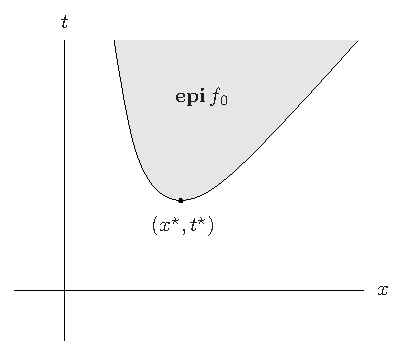
\includegraphics[width=.50\textwidth]{figures/ch04-01.pdf}
\caption*{图4.1\quad 无约束问题的上图形式的几何解释。问题是在上图（阴影部分）中寻找使 $t$ 最小的点，即上图中“最低”的点。最优点为 $(x^\star,t^\star)$。}
\end{figure}
从某些方面说，变换还使问题更困难。例如，假设原问题的目标 $f_0$ 可微，因而其定义域是开集。限制定义域后的目标 $F$ 很可能不可微，因为其定义域很可能不是开集。

反过来，我们也会遇到含有隐式约束的问题，并将其显式化。作为简单例子，考虑无约束问题
\begin{equation}
\text{最小化}\quad f(x),\tag{4.13}
\end{equation}
其中函数 $f$ 为
\[
f(x)=\begin{cases}x^\T x,&Ax=b,\\\infty,&\text{其他情形。}\end{cases}
\]
因此，目标函数在 $Ax=b$ 定义的仿射集上等于二次型 $x^\T x$，在仿射集之外等于 $\infty$。由于显然可以只考虑满足 $Ax=b$ 的点，我们说问题（4.13）的目标中隐藏着一个隐式等式约束 $Ax=b$。可将它显式化，形成等价问题
\begin{equation}
\begin{array}{ll}\text{最小化}&x^\T x\\\text{约束为}&Ax=b.\end{array}\tag{4.14}
\end{equation}
问题（4.13）和（4.14）显然等价，但并不相同。（4.13）无约束，但目标函数不可微；（4.14）有一个等式约束，但目标函数和约束函数均可微。

% Source PDF page 150 (printed p. 136)
\subsection{参数描述与预言机描述}
对于标准形式问题（4.1），还需要说明如何给定目标函数和约束函数。在许多情况下，这些函数有解析表达式或闭式表达式，即由涉及变量 $x$ 和若干参数的公式给出。例如，二次目标函数形如 $f_0(x)=(1/2)x^\T Px+q^\T x+r$。要给定目标函数，只需给出系数（也称问题参数或问题数据）$P\in\mathbf S^n$、$q\in\R^n$ 和 $r\in\R$。我们称其为参数化问题描述，因为要解的具体问题（即问题实例）由目标函数和约束函数表达式中各参数的取值给定。

在另一些情况下，目标函数和约束函数由预言机模型（也称黑箱模型或子程序模型）描述。在预言机模型中，我们不知道 $f$ 的显式表达式，但可以在任意 $x\in\dom f$ 处计算 $f(x)$（通常还包括某些导数）。这称为查询预言机，通常伴随某种成本，例如时间。我们还知道函数的一些先验信息，如凸性和函数值的界。作为具体例子，考虑最小化函数 $f$ 的无约束问题。函数值 $f(x)$ 和梯度 $\nabla f(x)$ 由一个子程序计算。我们可以在任意 $x\in\dom f$ 处调用子程序，但无法访问源代码。以 $x$ 为参数调用后，子程序返回 $f(x)$ 和 $\nabla f(x)$。注意，在预言机模型中，我们从未真正知道函数本身，只知道查询过的点上的函数值（及某些导数）。（另外还知道给定的先验信息，如可微性和凸性。）

实践中，参数描述与预言机描述之间的区别并不那么鲜明。如果给定参数描述，就可以构造一个预言机，在查询时计算所需函数值和导数。第三部分研究的大多数算法都采用预言机模型，但若限定只求解某个特定的参数化问题族，通常可以提高效率。

\section{凸优化}
\subsection{标准形式凸优化问题}
凸优化问题具有如下形式：
\begin{equation}
\begin{array}{ll}
\text{最小化}&f_0(x)\\
\text{约束为}&f_i(x)\le0,\quad i=1,\ldots,m,\\
&a_i^\T x=b_i,\quad i=1,\ldots,p,
\end{array}\tag{4.15}
\end{equation}
其中 $f_0,\ldots,f_m$ 为凸函数。与一般的标准形式问题（4.1）相比，凸问题额外要求以下三点：

% Source PDF page 151 (printed p. 137)
\begin{itemize}
\item 目标函数必须是凸函数；
\item 不等式约束函数必须是凸函数；
\item 等式约束函数 $h_i(x)=a_i^\T x-b_i$ 必须是仿射函数。
\end{itemize}
由此立即得到一个重要性质：凸优化问题的可行集是凸集，因为它是问题定义域
\[
\mathcal D=\bigcap_{i=0}^m\dom f_i
\]
与 $m$ 个凸下水平集 $\{x\mid f_i(x)\le0\}$ 以及 $p$ 个超平面 $\{x\mid a_i^\T x=b_i\}$ 的交，而定义域本身也是凸集。（不失一般性，可假设 $a_i\ne0$：若某个 $i$ 满足 $a_i=0$、$b_i=0$，可删除第 $i$ 个等式约束；若 $a_i=0$、$b_i\ne0$，该等式约束不相容，问题不可行。）因此，在凸优化问题中，我们在凸集上最小化凸目标函数。

若 $f_0$ 是拟凸而非凸函数，就称问题（4.15）为标准形式拟凸优化问题。由于凸函数或拟凸函数的下水平集是凸集，可知凸优化或拟凸优化问题的 $\epsilon$ 次优集均为凸集。特别地，最优集是凸集。若目标严格凸，则最优集至多包含一个点。

\subsubsection*{凹函数最大化问题}
若 $f_0$ 凹，而不等式约束函数 $f_1,\ldots,f_m$ 凸，我们也稍微放宽用语，将
\begin{equation}
\begin{array}{ll}
\text{最大化}&f_0(x)\\
\text{约束为}&f_i(x)\le0,\quad i=1,\ldots,m,\\
&a_i^\T x=b_i,\quad i=1,\ldots,p
\end{array}\tag{4.16}
\end{equation}
称为凸优化问题。这个凹函数最大化问题可以通过最小化凸目标 $-f_0$ 容易地求解。我们针对最小化问题介绍的全部结果、结论和算法，都容易转到最大化情形。类似地，当 $f_0$ 为拟凹函数时，也称最大化问题（4.16）为拟凸问题。

\subsubsection*{抽象形式的凸优化问题}
凸优化问题的定义中有一点细微之处值得注意。考虑变量为 $x\in\R^2$ 的例子
\begin{equation}
\begin{array}{ll}
\text{最小化}&f_0(x)=x_1^2+x_2^2\\
\text{约束为}&f_1(x)=x_1/(1+x_2^2)\le0,\\
&h_1(x)=(x_1+x_2)^2=0.
\end{array}\tag{4.17}
\end{equation}
它具有标准形式（4.1）。此问题并不是标准形式凸优化问题，因为等式约束函数 $h_1$ 不是仿射函数，不等式约束函数 $f_1$ 也不是凸函数。

% Source PDF page 152 (printed p. 138)
但可行集 $\{x\mid x_1\le0,\ x_1+x_2=0\}$ 是凸集。因此，虽然此问题是在凸集上最小化凸函数 $f_0$，按照我们的定义，它仍不是凸优化问题。

当然，很容易把问题重新写为
\begin{equation}
\begin{array}{ll}
\text{最小化}&f_0(x)=x_1^2+x_2^2\\
\text{约束为}&\widetilde f_1(x)=x_1\le0,\\
&\widetilde h_1(x)=x_1+x_2=0,
\end{array}\tag{4.18}
\end{equation}
它具有标准凸优化形式，因为 $f_0$ 和 $\widetilde f_1$ 凸，而 $\widetilde h_1$ 仿射。

有些作者用“抽象凸优化问题”表示在凸集上最小化凸函数这一抽象问题。采用这种术语，问题（4.17）就是抽象凸优化问题。本书不采用这种术语。对我们而言，凸优化问题不仅是在凸集上最小化凸函数；还要求可行集由涉及凸函数的一组不等式和一组线性等式约束具体描述。问题（4.17）不是凸优化问题，而（4.18）是凸优化问题。（不过这两个问题是等价的。）

我们采用较严格的凸优化问题定义，在实践中影响不大。为求解在凸集上最小化凸函数的抽象问题，需要用凸不等式和线性等式约束描述该集合。如上例所示，这通常很直接。

\subsection{局部最优与全局最优}
凸优化问题的一项基本性质是：任何局部最优点也是全局最优点。为说明这一点，设 $x$ 为凸优化问题的局部最优点，即 $x$ 可行，且存在 $R>0$，使
\begin{equation}
f_0(x)=\inf\{f_0(z)\mid z\text{ 可行},\ \norm{z-x}_2\le R\}.\tag{4.19}
\end{equation}
假设 $x$ 不是全局最优点，即存在可行点 $y$ 满足 $f_0(y)<f_0(x)$。显然 $\norm{y-x}_2>R$，否则有 $f_0(x)\le f_0(y)$。考虑点
\[
z=(1-\theta)x+\theta y,\qquad\theta=\frac{R}{2\norm{y-x}_2}.
\]
此时 $\norm{z-x}_2=R/2<R$，且由可行集的凸性，$z$ 可行。又由 $f_0$ 的凸性，
\[
f_0(z)\le(1-\theta)f_0(x)+\theta f_0(y)<f_0(x),
\]
这与（4.19）矛盾。因此不存在满足 $f_0(y)<f_0(x)$ 的可行点 $y$，即 $x$ 全局最优。

% Source PDF page 153 (printed p. 139)
\begin{figure}[htbp]
\centering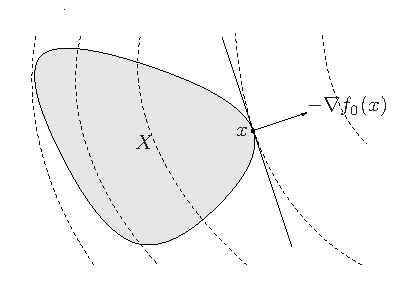
\includegraphics[width=.50\textwidth]{figures/ch04-02.pdf}
\caption*{图4.2\quad 最优性条件（4.21）的几何解释。阴影部分为可行集 $X$，虚线为 $f_0$ 的若干等高线。点 $x$ 最优：$-\nabla f_0(x)$ 在 $x$ 处定义了 $X$ 的一个支撑超平面（实线）。}
\end{figure}
拟凸优化问题的局部最优点不一定全局最优，见§4.2.5。

\subsection{可微目标函数 \texorpdfstring{$f_0$}{f0} 的最优性准则}
设凸优化问题的目标 $f_0$ 可微，因此对所有 $x,y\in\dom f_0$，有
\begin{equation}
f_0(y)\ge f_0(x)+\nabla f_0(x)^\T(y-x)\tag{4.20}
\end{equation}
（见§3.1.3）。用 $X$ 表示可行集，即
\[
X=\{x\mid f_i(x)\le0,\ i=1,\ldots,m,\ h_i(x)=0,\ i=1,\ldots,p\}.
\]
则 $x$ 最优，当且仅当 $x\in X$ 且
\begin{equation}
\nabla f_0(x)^\T(y-x)\ge0\qquad\text{对所有 }y\in X.\tag{4.21}
\end{equation}
这一最优性准则的几何意义是：若 $\nabla f_0(x)\ne0$，则 $-\nabla f_0(x)$ 在 $x$ 处定义可行集的一个支撑超平面，见图4.2。

\subsubsection*{最优性条件的证明}
先设 $x\in X$ 且满足（4.21）。对 $y\in X$，由（4.20）有 $f_0(y)\ge f_0(x)$。因此 $x$ 是问题（4.1）的最优点。

反过来，设 $x$ 最优，但条件（4.21）不成立，即存在 $y\in X$，使
\[
\nabla f_0(x)^\T(y-x)<0.
\]

% Source PDF page 154 (printed p. 140)
考虑点 $z(t)=ty+(1-t)x$，参数 $t\in[0,1]$。由于 $z(t)$ 位于 $x,y$ 之间的线段上，而可行集凸，所以 $z(t)$ 可行。我们断言，对充分小的正数 $t$，有 $f_0(z(t))<f_0(x)$，从而证明 $x$ 不最优。为此注意
\[
\left.\frac{d}{dt}f_0(z(t))\right|_{t=0}=\nabla f_0(x)^\T(y-x)<0,
\]
所以对充分小的正数 $t$，有 $f_0(z(t))<f_0(x)$。

第5章将更深入地研究最优性条件，这里先看几个简单例子。

\subsubsection*{无约束问题}
对于无约束问题，即 $m=p=0$，条件（4.21）化为熟知的最优性充要条件
\begin{equation}
\nabla f_0(x)=0.\tag{4.22}
\end{equation}
虽然我们已经见过这个最优性条件，仍有必要看看如何由（4.21）推出它。设 $x$ 最优，这里意味着 $x\in\dom f_0$，且对所有可行的 $y$ 有 $\nabla f_0(x)^\T(y-x)\ge0$。由于 $f_0$ 可微，其定义域按定义为开集，所以充分接近 $x$ 的所有 $y$ 都可行。取 $y=x-t\nabla f_0(x)$，其中 $t\in\R$ 为参数。$t$ 充分小且为正时，$y$ 可行，因此
\[
\nabla f_0(x)^\T(y-x)=-t\norm{\nabla f_0(x)}_2^2\ge0,
\]
从而 $\nabla f_0(x)=0$。

根据方程（4.22）解的个数，可能有几种情形。若（4.22）无解，就没有最优点，问题的最优值不能达到。这又可分为两种情形：问题无下界；或最优值有限但不能达到。另一方面，方程（4.22）也可能有多个解，此时每个解都是 $f_0$ 的最小点。

\begin{origexample}{4.5}
\textbf{无约束二次优化。}考虑最小化二次函数
\[
f_0(x)=(1/2)x^\T Px+q^\T x+r,
\]
其中 $P\in\mathbf S_+^n$，因此 $f_0$ 凸。$x$ 为 $f_0$ 最小点的充要条件是
\[
\nabla f_0(x)=Px+q=0.
\]
根据这个线性方程无解、有唯一解或有多个解，可能出现以下情形。
\begin{itemize}
\item 若 $q\notin\mathcal R(P)$，则无解。此时 $f_0$ 无下界。
\item 若 $P\succ0$（这也是 $f_0$ 严格凸的条件），则有唯一最小点 $x^\star=-P^{-1}q$。
% Source PDF page 155 (printed p. 141)
\item 若 $P$ 奇异，但 $q\in\mathcal R(P)$，则最优点构成仿射集 $X_{\mathrm{opt}}=-P^\dagger q+\mathcal N(P)$，其中 $P^\dagger$ 为 $P$ 的伪逆，见§A.5.4。
\end{itemize}
\end{origexample}

\begin{origexample}{4.6}
\textbf{解析中心。}考虑最小化凸函数 $f_0:\R^n\to\R$ 的无约束问题，其中
\[
f_0(x)=-\sum_{i=1}^m\log(b_i-a_i^\T x),\qquad\dom f_0=\{x\mid Ax\prec b\},
\]
$a_1^\T,\ldots,a_m^\T$ 为 $A$ 的各行。函数 $f_0$ 可微，所以 $x$ 最优的充要条件是
\begin{equation}
Ax\prec b,\qquad\nabla f_0(x)=\sum_{i=1}^m\frac{1}{b_i-a_i^\T x}a_i=0.\tag{4.23}
\end{equation}
（条件 $Ax\prec b$ 就是 $x\in\dom f_0$。）若 $Ax\prec b$ 不可行，则 $f_0$ 的定义域为空。假设 $Ax\prec b$ 可行，仍有以下几种可能，见习题4.2。
\begin{itemize}
\item （4.23）无解，因而问题没有最优点。当且仅当 $f_0$ 无下界时出现这种情形。
\item （4.23）有多个解。此时可以证明，解构成仿射集。
\item （4.23）有唯一解，即 $f_0$ 有唯一最小点。当且仅当开多面体 $\{x\mid Ax\prec b\}$ 非空且有界时出现这种情形。
\end{itemize}
\end{origexample}

\subsubsection*{只有等式约束的问题}
考虑有等式约束、没有不等式约束的情形，即
\[
\begin{array}{ll}\text{最小化}&f_0(x)\\\text{约束为}&Ax=b.\end{array}
\]
此时可行集是仿射集。假设它非空，否则问题不可行。对可行点 $x$，最优性条件要求
\[
\nabla f_0(x)^\T(y-x)\ge0
\]
对所有满足 $Ay=b$ 的 $y$ 成立。由于 $x$ 可行，每个可行点 $y$ 都可写为 $y=x+v$，其中 $v\in\mathcal N(A)$。所以最优性条件可以表示为
\[
\nabla f_0(x)^\T v\ge0\qquad\text{对所有 }v\in\mathcal N(A).
\]
一个线性函数若在子空间上非负，就必在该子空间上为零，所以对所有 $v\in\mathcal N(A)$ 有 $\nabla f_0(x)^\T v=0$。换言之，
\[
\nabla f_0(x)\perp\mathcal N(A).
\]

% Source PDF page 156 (printed p. 142)
利用 $\mathcal N(A)^\perp=\mathcal R(A^\T)$，最优性条件可写为 $\nabla f_0(x)\in\mathcal R(A^\T)$，即存在 $\nu\in\R^p$ 使
\[
\nabla f_0(x)+A^\T\nu=0.
\]
连同 $Ax=b$（即 $x$ 可行），这就是经典的拉格朗日乘子最优性条件，第5章将进一步研究。

\subsubsection*{非负正交象限上的最小化}
另一个例子是
\[
\begin{array}{ll}\text{最小化}&f_0(x)\\\text{约束为}&x\succeq0,\end{array}
\]
其中唯一的不等式约束是变量的非负约束。最优性条件（4.21）变为
\[
x\succeq0,\qquad\nabla f_0(x)^\T(y-x)\ge0\quad\text{对所有 }y\succeq0.
\]
除非 $\nabla f_0(x)\succeq0$，否则 $y$ 的线性函数 $\nabla f_0(x)^\T y$ 在 $y\succeq0$ 上无下界。于是条件化为 $-\nabla f_0(x)^\T x\ge0$。又由于 $x\succeq0$、$\nabla f_0(x)\succeq0$，必有 $\nabla f_0(x)^\T x=0$，即
\[
\sum_{i=1}^n(\nabla f_0(x))_ix_i=0.
\]
和式中每一项都是两个非负数的乘积，故每一项必为零，即 $(\nabla f_0(x))_ix_i=0$（$i=1,\ldots,n$）。所以最优性条件为
\[
x\succeq0,\qquad\nabla f_0(x)\succeq0,\qquad x_i(\nabla f_0(x))_i=0,\quad i=1,\ldots,n.
\]
最后一个条件称为互补性，因为它意味着向量 $x$ 和 $\nabla f_0(x)$ 的稀疏模式（非零分量对应的指标集合）互补，即交集为空。第5章还会遇到互补性条件。

\subsection{等价的凸问题}
了解§4.1.3中的哪些变换保持凸性是有用的。

\subsubsection*{消去等式约束}
凸问题的等式约束必须是线性的，即形如 $Ax=b$。此时，求一个特解 $x_0$ 和一个值域等于 $A$ 的零空间的矩阵 $F$，就可以消去等式约束，得到以 $z$ 为变量的问题

% Source PDF page 157 (printed p. 143)
\[
\begin{array}{ll}\text{最小化}&f_0(Fz+x_0)\\\text{约束为}&f_i(Fz+x_0)\le0,\quad i=1,\ldots,m.\end{array}
\]
由于凸函数与仿射函数复合仍凸，消去等式约束保持问题的凸性。此外，消去等式约束，以及由变换后问题的解恢复原问题的解，都只涉及标准线性代数运算。

至少在原则上，这意味着可以只考虑没有等式约束的凸优化问题。但许多情况下，保留等式约束更好，因为消去它们可能使问题更难理解和分析，或破坏求解算法的效率。例如，变量 $x$ 的维数很大，而消去等式约束会破坏问题的稀疏性或其他有用结构时，就会如此。

\subsubsection*{引入等式约束}
可以在凸优化问题中引入新变量和等式约束；只要这些等式约束是线性的，所得问题仍为凸问题。例如，若某个目标函数或约束函数形如 $f_i(A_ix+b_i)$，其中 $A_i\in\R^{k_i\times n}$，可引入新变量 $y_i\in\R^{k_i}$，用 $f_i(y_i)$ 替换 $f_i(A_ix+b_i)$，并加入线性等式约束 $y_i=A_ix+b_i$。

\subsubsection*{松弛变量}
引入松弛变量会产生新约束 $f_i(x)+s_i=0$。由于凸问题的等式约束函数必须是仿射函数，$f_i$ 必须仿射。换言之，为线性不等式引入松弛变量保持问题的凸性。

\subsubsection*{上图形式}
凸优化问题（4.15）的上图形式为
\[
\begin{array}{ll}
\text{最小化}&t\\
\text{约束为}&f_0(x)-t\le0,\\
&f_i(x)\le0,\quad i=1,\ldots,m,\\
&a_i^\T x=b_i,\quad i=1,\ldots,p.
\end{array}
\]
目标线性，因而凸；新约束函数 $f_0(x)-t$ 关于 $(x,t)$ 也凸，所以上图形式问题仍凸。

有时说线性目标对凸优化具有通用性，因为任何凸优化问题都容易变成具有线性目标的问题。凸问题的上图形式有若干实际用途。假定凸优化问题的目标线性，可以简化理论分析；也可以简化算法设计，因为求解线性目标凸优化问题的算法，借助上述变换，就能求解任意凸优化问题，只要它能够处理约束 $f_0(x)-t\le0$。

% Source PDF page 158 (printed p. 144)
\subsubsection*{对部分变量最小化}
对凸函数的部分变量最小化保持凸性。所以，若（4.9）中的 $f_0$ 关于 $x_1,x_2$ 联合凸，并且 $f_i$（$i=1,\ldots,m_1$）和 $\widetilde f_i$（$i=1,\ldots,m_2$）都凸，则等价问题（4.10）是凸问题。

\subsection{拟凸优化}
回顾标准形式的拟凸优化问题：
\begin{equation}
\begin{array}{ll}
\text{最小化}&f_0(x)\\
\text{约束为}&f_i(x)\le0,\quad i=1,\ldots,m,\\
&Ax=b,
\end{array}\tag{4.24}
\end{equation}
其中不等式约束函数 $f_1,\ldots,f_m$ 凸，目标 $f_0$ 拟凸，而凸优化问题要求目标凸。（拟凸约束函数可以用具有相同零下水平集的等价凸约束函数替换，见§3.4.5。）

本节指出凸优化与拟凸优化的一些基本区别，并说明如何将求解拟凸优化问题化为求解一系列凸优化问题。

\subsubsection*{局部最优解与最优性条件}
凸优化与拟凸优化最重要的区别是：拟凸优化问题可能存在并非全局最优的局部最优解。即使在 $\R$ 上无约束最小化拟凸函数的简单情形下，也能出现这一现象，如图4.3所示。

不过，§4.2.3中最优性条件（4.21）的一种变体，对目标可微的拟凸优化问题仍成立。以 $X$ 表示拟凸优化问题（4.24）的可行集。由拟凸性的一阶条件（3.20）可知，若
\begin{equation}
x\in X,\qquad\nabla f_0(x)^\T(y-x)>0\quad\text{对所有 }y\in X\setminus\{x\},\tag{4.25}
\end{equation}
则 $x$ 最优。与凸优化的对应准则（4.21）相比，有两个重要区别。
\begin{itemize}
\item 条件（4.25）只是最优性的充分条件；简单例子即可说明它对最优点未必成立。相比之下，（4.21）是 $x$ 解出凸问题的充要条件。
\item 条件（4.25）要求 $f_0$ 的梯度非零，而（4.21）没有这一要求。事实上，在凸情形下，$\nabla f_0(x)=0$ 时满足（4.21），$x$ 最优。
\end{itemize}

% Source PDF page 159 (printed p. 145)
\begin{figure}[htbp]
\centering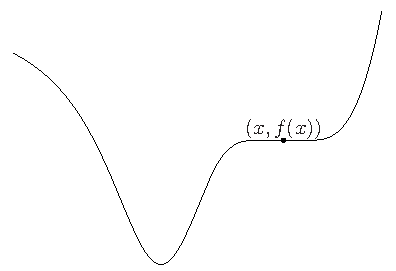
\includegraphics[width=.50\textwidth]{figures/ch04-03.pdf}
\caption*{图4.3\quad $\R$ 上的一个拟凸函数 $f$，其中局部最优点 $x$ 并非全局最优。这个例子说明，对凸函数有效的简单最优性条件 $f'(x)=0$，对拟凸函数并不成立。}
\end{figure}

\subsubsection*{通过凸可行性问题求解拟凸优化}
拟凸优化的一种一般方法，利用§3.4.5介绍的凸不等式族来表示拟凸函数的下水平集。设 $\phi_t:\R^n\to\R$（$t\in\R$）是一族凸函数，满足
\[
f_0(x)\le t\quad\Longleftrightarrow\quad\phi_t(x)\le0,
\]
而且对每个 $x$，$\phi_t(x)$ 关于 $t$ 非增，即 $s\ge t$ 时 $\phi_s(x)\le\phi_t(x)$。

以 $p^\star$ 表示拟凸优化问题（4.24）的最优值。如果可行性问题
\begin{equation}
\begin{array}{ll}
\text{求}&x\\
\text{使得}&\phi_t(x)\le0,\\
&f_i(x)\le0,\quad i=1,\ldots,m,\\
&Ax=b
\end{array}\tag{4.26}
\end{equation}
可行，则 $p^\star\le t$。反之，若（4.26）不可行，则 $p^\star\ge t$。问题（4.26）是凸可行性问题，因为全部不等式约束函数都凸，等式约束为线性。因此，可以通过求解凸可行性问题（4.26），判断拟凸优化问题的最优值 $p^\star$ 比给定值 $t$ 大还是小。若凸可行性问题可行，则 $p^\star\le t$，且任一可行点 $x$ 都对拟凸问题可行，并满足 $f_0(x)\le t$。若凸可行性问题不可行，则 $p^\star\ge t$。

这一观察可以构成一个简单的二分算法来求解拟凸优化问题（4.24），每一步解一个凸可行性问题。假设问题可行，先取一个已知包含最优值 $p^\star$ 的区间 $[l,u]$。在中点 $t=(l+u)/2$ 处求解凸可行性问题，判断最优值位于区间的下半段还是上半段，并据此更新区间。

% Source PDF page 160 (printed p. 146)
新区间仍包含最优值，但宽度只有原来的一半。重复这一过程，直到区间宽度足够小：

\begin{origalgorithm}{4.1}
\textbf{拟凸优化的二分法。}

给定 $l\le p^\star$、$u\ge p^\star$、容差 $\epsilon>0$。

重复：
\begin{enumerate}
\item $t:=(l+u)/2$。
\item 求解凸可行性问题（4.26）。
\item 若（4.26）可行，令 $u:=t$；否则令 $l:=t$。
\end{enumerate}
直到 $u-l\le\epsilon$。
\end{origalgorithm}

区间 $[l,u]$ 保证包含 $p^\star$，即每一步都有 $l\le p^\star\le u$。每轮将区间一分为二，因此 $k$ 轮后的区间长度为 $2^{-k}(u-l)$，这里 $u-l$ 指初始区间长度。由此可知，算法终止前恰需 $\lceil\log_2((u-l)/\epsilon)\rceil$ 轮。每一步都要求解凸可行性问题（4.26）。

\section{线性优化问题}
当目标函数和约束函数均为仿射函数时，问题称为线性规划（LP）。一般线性规划的形式为
\begin{equation}
\begin{array}{ll}
\text{最小化}&c^\T x+d\\
\text{约束为}&Gx\preceq h,\\
&Ax=b,
\end{array}\tag{4.27}
\end{equation}
其中 $G\in\R^{m\times n}$、$A\in\R^{p\times n}$。线性规划当然是凸优化问题。

由于目标中的常数 $d$ 不影响最优集或可行集，通常将它省略。仿射目标 $c^\T x+d$ 的最大化可以通过最小化 $-c^\T x-d$ 完成，后者仍凸，因此也把目标和约束函数均为仿射函数的最大化问题称为LP。

LP的几何意义如图4.4所示。LP（4.27）的可行集是多面体 $\mathcal P$；问题是在 $\mathcal P$ 上最小化仿射函数 $c^\T x+d$，或等价地最小化线性函数 $c^\T x$。

\subsubsection*{标准形式与不等式形式的线性规划}
LP（4.27）有两种非常常见的特殊情形，各有专门名称。标准形式LP中，唯一的不等式是逐分量非负约束 $x\succeq0$：

% Source PDF page 161 (printed p. 147)
\begin{figure}[htbp]
\centering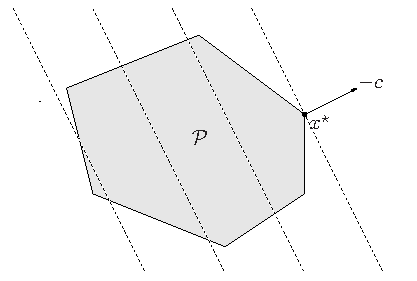
\includegraphics[width=.50\textwidth]{figures/ch04-04.pdf}
\caption*{图4.4\quad LP的几何解释。阴影部分为多面体可行集 $\mathcal P$。目标 $c^\T x$ 线性，所以其等高线是垂直于 $c$ 的超平面（虚线）。点 $x^\star$ 最优，它是 $\mathcal P$ 中沿 $-c$ 方向最远的点。}
\end{figure}
\begin{equation}
\begin{array}{ll}\text{最小化}&c^\T x\\\text{约束为}&Ax=b,\\&x\succeq0.\end{array}\tag{4.28}
\end{equation}
若LP没有等式约束，称为不等式形式LP，通常写为
\begin{equation}
\begin{array}{ll}\text{最小化}&c^\T x\\\text{约束为}&Ax\preceq b.\end{array}\tag{4.29}
\end{equation}

\subsubsection*{将LP转化为标准形式}
有时将一般LP（4.27）转化为标准形式（4.28）很有用，例如为了使用求解标准形式LP的算法。第一步为不等式引入松弛变量 $s_i$，得到
\[
\begin{array}{ll}\text{最小化}&c^\T x+d\\\text{约束为}&Gx+s=h,\\&Ax=b,\\&s\succeq0.\end{array}
\]
第二步将变量 $x$ 表示为两个非负变量 $x^+$、$x^-$ 的差，即 $x=x^+-x^-$，$x^+,x^-\succeq0$，得到
\[
\begin{array}{ll}
\text{最小化}&c^\T x^+-c^\T x^-+d\\
\text{约束为}&Gx^+-Gx^-+s=h,\\
&Ax^+-Ax^-=b,\\
&x^+\succeq0,\quad x^-\succeq0,\quad s\succeq0.
\end{array}
\]

% Source PDF page 162 (printed p. 148)
这是以 $x^+,x^-,s$ 为变量的标准形式LP。（此问题与原问题（4.27）的等价性见习题4.10。）

这些问题变换技巧，加上后面的例子和习题中会介绍的许多其他技巧，可以将大量问题表述为线性规划。用语上常作一定放宽：即使一个问题本身不具有（4.27）的形式，只要能表述为LP，通常也将其称为LP。

\subsection{例子}
LP出现在大量领域和应用中，下面给出几个典型例子。

\subsubsection*{膳食问题}
健康膳食需要包含 $m$ 种不同营养素，其数量至少分别为 $b_1,\ldots,b_m$。可从 $n$ 种食物中选择非负数量 $x_1,\ldots,x_n$，组成这种膳食。每单位食物 $j$ 含有数量为 $a_{ij}$ 的营养素 $i$，成本为 $c_j$。我们要确定满足营养要求的最便宜膳食。此问题可表述为LP
\[
\begin{array}{ll}\text{最小化}&c^\T x\\\text{约束为}&Ax\succeq b,\\&x\succeq0.\end{array}
\]
这个问题的若干变体也可以表述为LP。例如，可要求某种营养素的数量精确等于指定值，从而得到线性等式约束；也可在上述下界之外，再对营养素的数量施加上界。

\subsubsection*{多面体的Chebyshev中心}
考虑在由线性不等式描述的多面体
\[
\mathcal P=\{x\in\R^n\mid a_i^\T x\le b_i,\ i=1,\ldots,m\}
\]
中寻找最大欧氏球的问题。（最优球的中心称为多面体的Chebyshev中心；它是多面体内部最深的点，即离边界最远的点，见§8.5.1。）将球表示为
\[
\mathcal B=\{x_c+u\mid\norm{u}_2\le r\}.
\]
问题的变量为球心 $x_c\in\R^n$ 和半径 $r$，目标是在 $\mathcal B\subseteq\mathcal P$ 的约束下最大化 $r$。

先考虑较简单的约束：$\mathcal B$ 位于一个半空间 $a_i^\T x\le b_i$ 中，即
\begin{equation}
\norm{u}_2\le r\quad\Longrightarrow\quad a_i^\T(x_c+u)\le b_i.\tag{4.30}
\end{equation}
由于
\[
\sup\{a_i^\T u\mid\norm{u}_2\le r\}=r\norm{a_i}_2,
\]

% Source PDF page 163 (printed p. 149)
可以将（4.30）写为
\begin{equation}
a_i^\T x_c+r\norm{a_i}_2\le b_i,\tag{4.31}
\end{equation}
它是关于 $x_c,r$ 的线性不等式。换言之，球包含于不等式 $a_i^\T x\le b_i$ 所确定半空间的约束，可以写成线性不等式。

所以 $\mathcal B\subseteq\mathcal P$ 当且仅当（4.31）对所有 $i=1,\ldots,m$ 成立。因此，求解LP
\[
\begin{array}{ll}\text{最大化}&r\\\text{约束为}&a_i^\T x_c+r\norm{a_i}_2\le b_i,\quad i=1,\ldots,m\end{array}
\]
即可确定Chebyshev中心，变量为 $r,x_c$。（更多关于Chebyshev中心的内容见§8.5.1。）

\subsubsection*{动态活动规划}
考虑在 $N$ 个时期内，为 $n$ 项活动或经济部门选择、规划活动水平的问题。以 $x_j(t)\ge0$（$t=1,\ldots,N$）表示部门 $j$ 在第 $t$ 期的活动水平。活动按其水平成比例地消耗和生产产品或物品。每单位活动 $j$ 生产的物品 $i$ 的数量为 $a_{ij}$；类似地，每单位活动 $j$ 消耗的物品 $i$ 的数量为 $b_{ij}$。第 $t$ 期的总产出为 $Ax(t)\in\R^m$，总消耗为 $Bx(t)\in\R^m$。（虽然称这些产品为“物品”，它们也可以包括污染物等不需要的产物。）

每期消耗的物品不能超过前一期生产的物品，即要求 $Bx(t+1)\preceq Ax(t)$（$t=1,\ldots,N$）。给定初始物品向量 $g_0\in\R^m$，它限制第一期活动水平：$Bx(1)\preceq g_0$。未被活动消耗的剩余物品向量为
\[
\begin{aligned}
s(0)&=g_0-Bx(1),\\
s(t)&=Ax(t)-Bx(t+1),\quad t=1,\ldots,N-1,\\
s(N)&=Ax(N).
\end{aligned}
\]
目标是最大化剩余物品的折现总价值：
\[
c^\T s(0)+\gamma c^\T s(1)+\cdots+\gamma^N c^\T s(N),
\]
其中 $c\in\R^m$ 给出物品的价值，$\gamma>0$ 为折现因子。（若第 $i$ 种产品是不需要的，例如污染物，则 $c_i$ 为负数，此时 $|c_i|$ 为单位处置成本。）

综上，得到LP
\[
\begin{array}{ll}
\text{最大化}&c^\T s(0)+\gamma c^\T s(1)+\cdots+\gamma^N c^\T s(N)\\
\text{约束为}&x(t)\succeq0,\quad t=1,\ldots,N,\\
&s(t)\succeq0,\quad t=0,\ldots,N,\\
&s(0)=g_0-Bx(1),\\
&s(t)=Ax(t)-Bx(t+1),\quad t=1,\ldots,N-1,\\
&s(N)=Ax(N),
\end{array}
\]
变量为 $x(1),\ldots,x(N),s(0),\ldots,s(N)$。这是标准形式LP，变量 $s(t)$ 是约束 $Bx(t+1)\preceq Ax(t)$ 对应的松弛变量。

% Source PDF page 164 (printed p. 150)
\subsubsection*{Chebyshev不等式}
考虑离散随机变量 $x$ 在有 $n$ 个元素的集合 $\{u_1,\ldots,u_n\}\subseteq\R$ 上的概率分布。以向量 $p\in\R^n$ 描述 $x$ 的分布，其中
\[
p_i=\Prob(x=u_i),
\]
因此 $p\succeq0$、$\one^\T p=1$。反过来，若 $p$ 满足这两个条件，它就定义了 $x$ 的一个概率分布。假设 $u_i$ 已知且固定，但分布 $p$ 未知。

对 $x$ 的任意函数 $f$，
\[
\E f=\sum_{i=1}^n p_if(u_i)
\]
是 $p$ 的线性函数。对 $\R$ 的任意子集 $S$，
\[
\Prob(x\in S)=\sum_{u_i\in S}p_i
\]
也是 $p$ 的线性函数。

虽然不知道 $p$，但给定如下先验知识：知道 $x$ 的某些函数的期望，以及某些 $\R$ 的子集的概率的上下界。这些先验知识可表示为关于 $p$ 的线性不等式约束
\[
\alpha_i\le a_i^\T p\le\beta_i,\quad i=1,\ldots,m.
\]
问题是为 $\E f_0(x)=a_0^\T p$ 给出上下界，其中 $f_0$ 是 $x$ 的某个函数。

为求下界，解以 $p$ 为变量的LP
\[
\begin{array}{ll}\text{最小化}&a_0^\T p\\\text{约束为}&p\succeq0,\quad\one^\T p=1,\\&\alpha_i\le a_i^\T p\le\beta_i,\quad i=1,\ldots,m.\end{array}
\]
这个LP的最优值给出了与先验信息相容的所有分布中 $\E f_0(X)$ 的最小可能值。而且此界是紧的：最优解给出一个与先验信息相容且达到下界的分布。类似地，在相同约束下最大化 $a_0^\T p$，可得最佳上界。（§7.4.1将更详细地讨论Chebyshev不等式。）

\subsubsection*{分段线性函数最小化}
考虑无约束最小化分段线性凸函数
\[
f(x)=\max_{i=1,\ldots,m}(a_i^\T x+b_i)
\]
的问题。先取上图形式
\[
\begin{array}{ll}\text{最小化}&t\\\text{约束为}&\max_{i=1,\ldots,m}(a_i^\T x+b_i)\le t,\end{array}
\]
再将不等式改写为 $m$ 个单独的不等式，即可变为等价LP：

% Source PDF page 165 (printed p. 151)
\[
\begin{array}{ll}\text{最小化}&t\\\text{约束为}&a_i^\T x+b_i\le t,\quad i=1,\ldots,m.\end{array}
\]
这是以 $x,t$ 为变量的不等式形式LP。

\subsection{线性分式规划}
在多面体上最小化两个仿射函数之比的问题，称为线性分式规划：
\begin{equation}
\begin{array}{ll}\text{最小化}&f_0(x)\\\text{约束为}&Gx\preceq h,\\&Ax=b,\end{array}\tag{4.32}
\end{equation}
其中目标为
\[
f_0(x)=\frac{c^\T x+d}{e^\T x+f},\qquad\dom f_0=\{x\mid e^\T x+f>0\}.
\]
目标函数拟凸，实际上是拟线性的，因此线性分式规划是拟凸优化问题。

\subsubsection*{转化为线性规划}
若可行集
\[
\{x\mid Gx\preceq h,\ Ax=b,\ e^\T x+f>0\}
\]
非空，线性分式规划（4.32）可转化为以 $y,z$ 为变量的等价LP
\begin{equation}
\begin{array}{ll}
\text{最小化}&c^\T y+dz\\
\text{约束为}&Gy-hz\preceq0,\\
&Ay-bz=0,\\
&e^\T y+fz=1,\\
&z\ge0.
\end{array}\tag{4.33}
\end{equation}
为说明等价性，先注意，若 $x$ 对（4.32）可行，则
\[
y=\frac{x}{e^\T x+f},\qquad z=\frac{1}{e^\T x+f}
\]
对（4.33）可行，且目标值相同，即 $c^\T y+dz=f_0(x)$。所以（4.32）的最优值大于等于（4.33）的最优值。

反过来，若 $(y,z)$ 对（4.33）可行且 $z\ne0$，则 $x=y/z$ 对（4.32）可行，且目标值相同：$f_0(x)=c^\T y+dz$。若 $(y,z)$ 对（4.33）可行且 $z=0$，另有 $x_0$ 对（4.32）可行，则对所有 $t\ge0$，$x=x_0+ty$ 对（4.32）可行。而且 $\lim_{t\to\infty}f_0(x_0+ty)=c^\T y+dz$，所以可找到（4.32）的可行点，使目标值任意接近 $(y,z)$ 的目标值。由此可知，（4.32）的最优值小于等于（4.33）的最优值。

% Source PDF page 166 (printed p. 152)
\subsubsection*{广义线性分式规划}
线性分式规划（4.32）的一种推广为广义线性分式规划，其中
\[
f_0(x)=\max_{i=1,\ldots,r}\frac{c_i^\T x+d_i}{e_i^\T x+f_i},\qquad
\dom f_0=\{x\mid e_i^\T x+f_i>0,\ i=1,\ldots,r\}.
\]
目标为 $r$ 个拟凸函数的逐点最大值，因而拟凸，所以此问题为拟凸问题。当 $r=1$ 时，它退化为普通线性分式规划。

\begin{origexample}{4.7}
\textbf{Von Neumann增长问题。}考虑有 $n$ 个部门的经济系统，当前期活动水平为 $x_i>0$，下一期为 $x_i^+>0$。（此处只考虑一个时期。）活动既消耗也生产 $m$ 种物品：活动水平 $x$ 消耗物品 $Bx\in\R^m$，生产物品 $Ax$。下一期消耗不能超过当前期产出，即 $Bx^+\preceq Ax$。部门 $i$ 在此期间的增长率为 $x_i^+/x_i$。

Von Neumann增长问题是寻找活动水平向量 $x$，使全部部门中的最小增长率最大。此问题可表示为广义线性分式问题
\[
\begin{array}{ll}\text{最大化}&\min_{i=1,\ldots,n}x_i^+/x_i\\\text{约束为}&x^+\succeq0,\\&Bx^+\preceq Ax,\end{array}
\]
定义域为 $\{(x,x^+)\mid x\succ0\}$。注意，此问题关于 $x,x^+$ 齐次，因此可用显式约束 $x\succeq\one$ 替换隐式约束 $x\succ0$。
\end{origexample}

\section{二次优化问题}
若凸优化问题（4.15）的目标为凸二次函数，约束函数为仿射函数，就称为二次规划（QP）。二次规划可表示为
\begin{equation}
\begin{array}{ll}\text{最小化}&(1/2)x^\T Px+q^\T x+r\\\text{约束为}&Gx\preceq h,\\&Ax=b,\end{array}\tag{4.34}
\end{equation}
其中 $P\in\mathbf S_+^n$、$G\in\R^{m\times n}$、$A\in\R^{p\times n}$。二次规划是在多面体上最小化凸二次函数，如图4.5。

若（4.15）的目标和不等式约束函数均为凸二次函数，如
\begin{equation}
\begin{array}{ll}
\text{最小化}&(1/2)x^\T P_0x+q_0^\T x+r_0\\
\text{约束为}&(1/2)x^\T P_ix+q_i^\T x+r_i\le0,\quad i=1,\ldots,m,\\
&Ax=b,
\end{array}\tag{4.35}
\end{equation}

% Source PDF page 167 (printed p. 153)
\begin{figure}[htbp]
\centering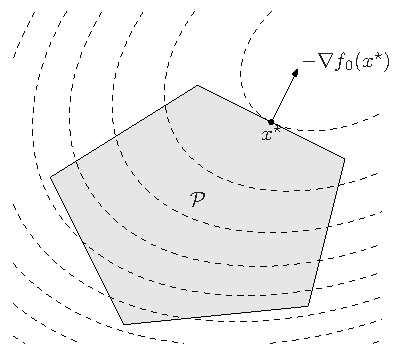
\includegraphics[width=.50\textwidth]{figures/ch04-05.pdf}
\caption*{图4.5\quad QP的几何示意。阴影部分为多面体可行集 $\mathcal P$，虚线为凸二次目标函数的等高线。点 $x^\star$ 最优。}
\end{figure}
其中 $P_i\in\mathbf S_+^n$（$i=0,1,\ldots,m$），就称为二次约束二次规划（QCQP）。QCQP在椭球的交构成的可行域上最小化凸二次函数，这里椭球情形对应 $P_i\succ0$。

二次规划包含线性规划这一特例，只需在（4.34）中取 $P=0$。二次约束二次规划包含二次规划，因而也包含线性规划这一特例，只需在（4.35）中对 $i=1,\ldots,m$ 取 $P_i=0$。

\subsection{例子}
\subsubsection*{最小二乘与回归}
最小化凸二次函数
\[
\norm{Ax-b}_2^2=x^\T A^\T Ax-2b^\T Ax+b^\T b
\]
的问题是无约束QP。它出现在许多领域，有许多名称，如回归分析或最小二乘逼近。这个问题足够简单，具有熟知的解析解 $x=A^\dagger b$，其中 $A^\dagger$ 为 $A$ 的伪逆，见§A.5.4。

加入线性不等式约束后，称为约束回归或约束最小二乘，此时不再有简单的解析解。例如，考虑对变量施加上下界的回归问题
\[
\begin{array}{ll}\text{最小化}&\norm{Ax-b}_2^2\\\text{约束为}&l_i\le x_i\le u_i,\quad i=1,\ldots,n,\end{array}
\]

% Source PDF page 168 (printed p. 154)
这是QP。（第6章和第7章将更深入研究最小二乘和回归问题。）

\subsubsection*{多面体之间的距离}
$\R^n$ 中两个多面体 $\mathcal P_1=\{x\mid A_1x\preceq b_1\}$ 与 $\mathcal P_2=\{x\mid A_2x\preceq b_2\}$ 的欧氏距离定义为
\[
\dist(\mathcal P_1,\mathcal P_2)=\inf\{\norm{x_1-x_2}_2\mid x_1\in\mathcal P_1,\ x_2\in\mathcal P_2\}.
\]
若两个多面体相交，距离为零。

为求 $\mathcal P_1$ 与 $\mathcal P_2$ 的距离，可解以 $x_1,x_2\in\R^n$ 为变量的QP
\[
\begin{array}{ll}\text{最小化}&\norm{x_1-x_2}_2^2\\\text{约束为}&A_1x_1\preceq b_1,\quad A_2x_2\preceq b_2.\end{array}
\]
当且仅当至少一个多面体为空时，此问题不可行。当且仅当两个多面体相交时，最优值为零，此时最优 $x_1,x_2$ 相等，并位于交集 $\mathcal P_1\cap\mathcal P_2$ 中。否则，最优 $x_1,x_2$ 分别是两个多面体中彼此距离最近的点。（第8章将进一步研究涉及距离的几何问题。）

\subsubsection*{方差的界}
再次考虑第150页Chebyshev不等式的例子，变量为向量 $p\in\R^n$ 给出的未知概率分布，已知它的一些先验信息。随机变量 $f(x)$ 的方差为
\[
\E f^2-(\E f)^2=\sum_{i=1}^n f_i^2p_i-\left(\sum_{i=1}^n f_ip_i\right)^2,
\]
其中 $f_i=f(u_i)$，它是 $p$ 的凹二次函数。

因此，在给定先验信息约束下最大化 $f(x)$ 的方差，可以求解QP
\[
\begin{array}{ll}
\text{最大化}&\displaystyle\sum_{i=1}^n f_i^2p_i-\left(\sum_{i=1}^n f_ip_i\right)^2\\
\text{约束为}&p\succeq0,\quad\one^\T p=1,\\
&\alpha_i\le a_i^\T p\le\beta_i,\quad i=1,\ldots,m.
\end{array}
\]
最优值是在全部与先验信息相容的分布中 $f(x)$ 的最大可能方差；最优 $p$ 给出达到该最大方差的分布。

\subsubsection*{随机成本的线性规划}
考虑以 $x\in\R^n$ 为变量的LP
\[
\begin{array}{ll}\text{最小化}&c^\T x\\\text{约束为}&Gx\preceq h,\\&Ax=b.\end{array}
\]

% Source PDF page 169 (printed p. 155)
假设成本向量 $c\in\R^n$ 为随机变量，均值为 $\bar c$，协方差为 $\E(c-\bar c)(c-\bar c)^\T=\Sigma$。（为简单起见，假设其余问题参数均为确定量。）给定 $x\in\R^n$，成本 $c^\T x$ 是标量随机变量，其均值为 $\E c^\T x=\bar c^\T x$，方差为
\[
\operatorname{var}(c^\T x)=\E(c^\T x-\E c^\T x)^2=x^\T\Sigma x.
\]
通常需要在较小的期望成本与较小的成本方差之间取舍。考虑方差的一种方式，是最小化成本期望和方差的线性组合
\[
\E c^\T x+\gamma\operatorname{var}(c^\T x),
\]
称为风险敏感成本。参数 $\gamma\ge0$ 称为风险厌恶参数，因为它规定成本方差与期望的相对价值。（$\gamma>0$ 时，我们愿意接受期望成本增加，以换取足够大的成本方差下降。）

最小化风险敏感成本，就是求解QP
\[
\begin{array}{ll}\text{最小化}&\bar c^\T x+\gamma x^\T\Sigma x\\\text{约束为}&Gx\preceq h,\\&Ax=b.\end{array}
\]

\subsubsection*{Markowitz投资组合优化}
考虑在一段时期内持有 $n$ 种资产或股票的经典投资组合问题。以 $x_i$ 表示整个时期持有的资产 $i$ 的数量，按期初价格以美元计。资产 $i$ 的普通多头头寸对应 $x_i>0$；空头头寸，即期末购买该资产的义务，对应 $x_i<0$。以 $p_i$ 表示该时期资产 $i$ 的相对价格变化，即价格变化除以期初价格。整个投资组合的收益为 $r=p^\T x$，单位为美元。优化变量为投资组合向量 $x\in\R^n$。

可以考虑多种投资组合约束。最简单的是 $x_i\ge0$（没有空头头寸）和 $\one^\T x=B$（总投资预算为 $B$，通常取一）。

采用价格变化的随机模型：$p\in\R^n$ 为随机向量，均值 $\bar p$ 和协方差 $\Sigma$ 已知。因此，对投资组合 $x\in\R^n$，收益 $r$ 为标量随机变量，均值为 $\bar p^\T x$，方差为 $x^\T\Sigma x$。选择投资组合 $x$ 就涉及收益均值与方差的取舍。

Markowitz提出的经典投资组合优化问题是QP
\[
\begin{array}{ll}\text{最小化}&x^\T\Sigma x\\\text{约束为}&\bar p^\T x\ge r_{\min},\\&\one^\T x=1,\quad x\succeq0,\end{array}
\]
其中投资组合 $x$ 为变量。这里寻找使收益方差最小的投资组合，收益方差与组合风险相关，同时要求达到可接受的最低平均收益 $r_{\min}$，并满足预算和禁止卖空约束。

% Source PDF page 170 (printed p. 156)
这个问题有许多推广。例如，一个标准推广是允许空头头寸，即允许 $x_i<0$。为此引入变量 $x^{\mathrm{long}},x^{\mathrm{short}}$，满足
\[
x^{\mathrm{long}}\succeq0,\quad x^{\mathrm{short}}\succeq0,\quad
x=x^{\mathrm{long}}-x^{\mathrm{short}},\quad
\one^\T x^{\mathrm{short}}\le\eta\one^\T x^{\mathrm{long}}.
\]
最后一个约束将期初总空头头寸限制为期初总多头头寸的某个比例 $\eta$。

另一个推广是在投资组合优化中计入线性交易成本。从给定初始投资组合 $x^{\mathrm{init}}$ 出发，通过买卖资产得到投资组合 $x$，然后按前述方式持有一个时期。买卖收取与交易数量成比例的交易费。为处理这一点，引入变量 $u^{\mathrm{buy}},u^{\mathrm{sell}}$，分别表示持有期开始前买入、卖出的各项资产数量，约束为
\[
x=x^{\mathrm{init}}+u^{\mathrm{buy}}-u^{\mathrm{sell}},\qquad
u^{\mathrm{buy}}\succeq0,\quad u^{\mathrm{sell}}\succeq0.
\]
用初始买卖包括交易费的净现金流为零，替换简单预算约束 $\one^\T x=1$：
\[
(1-f^{\mathrm{sell}})\one^\T u^{\mathrm{sell}}
=(1+f^{\mathrm{buy}})\one^\T u^{\mathrm{buy}}.
\]
左侧是卖出资产的总收入减去卖出交易费，右侧是买入资产包括交易费的总成本。常数 $f^{\mathrm{buy}}\ge0$、$f^{\mathrm{sell}}\ge0$ 分别为买入和卖出的费率，为简单起见，假设所有资产费率相同。

在最低平均收益、预算及交易约束下，最小化收益方差，是以 $x,u^{\mathrm{buy}},u^{\mathrm{sell}}$ 为变量的QP。

\subsection{二阶锥规划}
与二次规划密切相关的一类问题是二阶锥规划（SOCP）：
\begin{equation}
\begin{array}{ll}
\text{最小化}&f^\T x\\
\text{约束为}&\norm{A_ix+b_i}_2\le c_i^\T x+d_i,\quad i=1,\ldots,m,\\
&Fx=g,
\end{array}\tag{4.36}
\end{equation}
其中优化变量为 $x\in\R^n$，$A_i\in\R^{n_i\times n}$，$F\in\R^{p\times n}$。形如
\[
\norm{Ax+b}_2\le c^\T x+d,
\]
其中 $A\in\R^{k\times n}$，的约束称为二阶锥约束，因为它等价于要求仿射函数 $(Ax+b,c^\T x+d)$ 位于 $\R^{k+1}$ 的二阶锥中。

当 $c_i=0$（$i=1,\ldots,m$）时，SOCP（4.36）等价于QCQP，将各个约束平方即可得到。类似地，若 $A_i=0$（$i=1,\ldots,m$），则（4.36）退化为一般LP。不过，二阶锥规划比QCQP更加一般，当然也比LP更加一般。

% Source PDF page 171 (printed p. 157)
\subsubsection*{鲁棒线性规划}
考虑不等式形式的线性规划
\[
\begin{array}{ll}\text{最小化}&c^\T x\\\text{约束为}&a_i^\T x\le b_i,\quad i=1,\ldots,m,\end{array}
\]
其中参数 $c,a_i,b_i$ 存在不确定性或变化。为简化叙述，假设 $c,b_i$ 固定，而已知 $a_i$ 位于给定椭球中：
\[
a_i\in\mathcal E_i=\{\bar a_i+P_iu\mid\norm{u}_2\le1\},
\]
其中 $P_i\in\R^{n\times n}$。（若 $P_i$ 奇异，得到维数为 $\rank P_i$ 的“扁平”椭球；$P_i=0$ 表示完全知道 $a_i$。）

我们要求对参数 $a_i$ 的所有可能取值，约束都成立，由此得到鲁棒线性规划
\begin{equation}
\begin{array}{ll}\text{最小化}&c^\T x\\\text{约束为}&a_i^\T x\le b_i\quad\text{对所有 }a_i\in\mathcal E_i,\quad i=1,\ldots,m.\end{array}\tag{4.37}
\end{equation}
鲁棒线性约束“对所有 $a_i\in\mathcal E_i$，有 $a_i^\T x\le b_i$”可写为
\[
\sup\{a_i^\T x\mid a_i\in\mathcal E_i\}\le b_i,
\]
其左侧为
\[
\begin{aligned}
\sup\{a_i^\T x\mid a_i\in\mathcal E_i\}
&=\bar a_i^\T x+\sup\{u^\T P_i^\T x\mid\norm{u}_2\le1\}\\
&=\bar a_i^\T x+\norm{P_i^\T x}_2.
\end{aligned}
\]
因此，鲁棒线性约束可以表示为
\[
\bar a_i^\T x+\norm{P_i^\T x}_2\le b_i,
\]
它显然是二阶锥约束。所以鲁棒LP（4.37）可表示为SOCP
\[
\begin{array}{ll}\text{最小化}&c^\T x\\\text{约束为}&\bar a_i^\T x+\norm{P_i^\T x}_2\le b_i,\quad i=1,\ldots,m.\end{array}
\]
注意，增加的范数项起着正则化作用；它们防止 $x$ 在参数 $a_i$ 不确定性较大的方向上取得过大的值。

\subsubsection*{带随机约束的线性规划}
上述鲁棒LP也可以在统计框架下考虑。假设参数 $a_i$ 是相互独立的高斯随机向量，均值为 $\bar a_i$、协方差为 $\Sigma_i$。要求每个约束 $a_i^\T x\le b_i$ 成立的概率或置信度超过 $\eta$，其中 $\eta\ge0.5$，即
\begin{equation}
\Prob(a_i^\T x\le b_i)\ge\eta.\tag{4.38}
\end{equation}

% Source PDF page 172 (printed p. 158)
我们将说明这个概率约束可表示为二阶锥约束。

令 $u=a_i^\T x$，以 $\sigma^2$ 表示其方差，则约束可写为
\[
\Prob\left(\frac{u-\bar u}{\sigma}\le\frac{b_i-\bar u}{\sigma}\right)\ge\eta.
\]
由于 $(u-\bar u)/\sigma$ 是零均值、单位方差的高斯变量，上述概率就是 $\Phi((b_i-\bar u)/\sigma)$，其中
\[
\Phi(z)=\frac1{\sqrt{2\pi}}\int_{-\infty}^z e^{-t^2/2}\,dt
\]
是零均值、单位方差高斯随机变量的累积分布函数。因此，概率约束（4.38）可表示为
\[
\frac{b_i-\bar u}{\sigma}\ge\Phi^{-1}(\eta),
\]
或等价地
\[
\bar u+\Phi^{-1}(\eta)\sigma\le b_i.
\]
利用 $\bar u=\bar a_i^\T x$、$\sigma=(x^\T\Sigma_i x)^{1/2}$，得到
\[
\bar a_i^\T x+\Phi^{-1}(\eta)\norm{\Sigma_i^{1/2}x}_2\le b_i.
\]
根据假设 $\eta\ge1/2$，有 $\Phi^{-1}(\eta)\ge0$，所以此约束为二阶锥约束。

综上，问题
\[
\begin{array}{ll}\text{最小化}&c^\T x\\\text{约束为}&\Prob(a_i^\T x\le b_i)\ge\eta,\quad i=1,\ldots,m\end{array}
\]
可表示为SOCP
\[
\begin{array}{ll}\text{最小化}&c^\T x\\\text{约束为}&\bar a_i^\T x+\Phi^{-1}(\eta)\norm{\Sigma_i^{1/2}x}_2\le b_i,\quad i=1,\ldots,m.\end{array}
\]
（第6章将更深入研究鲁棒凸优化问题，另见习题4.13、4.28和4.59。）

\begin{origexample}{4.8}
\textbf{带损失风险约束的投资组合优化。}再次考虑前述经典Markowitz投资组合问题，见第155页。这里假设价格变化向量 $p\in\R^n$ 是高斯随机变量，均值为 $\bar p$、协方差为 $\Sigma$。因此收益 $r$ 是高斯随机变量，其均值为 $\bar r=\bar p^\T x$，方差为 $\sigma_r^2=x^\T\Sigma x$。

考虑形如
\begin{equation}
\Prob(r\le\alpha)\le\beta\tag{4.39}
\end{equation}
的损失风险约束，其中 $\alpha$ 是给定的不希望出现的收益水平，例如较大的损失，$\beta$ 是给定的最大概率。

% Source PDF page 173 (printed p. 159)
与上述鲁棒LP的随机解释类似，可以用单位高斯随机变量的累积分布函数 $\Phi$ 表达此约束。不等式（4.39）等价于
\[
\bar p^\T x+\Phi^{-1}(\beta)\norm{\Sigma^{1/2}x}_2\ge\alpha.
\]
只要 $\beta\le1/2$，即 $\Phi^{-1}(\beta)\le0$，此损失风险约束就是二阶锥约束。（若 $\beta>1/2$，损失风险约束关于 $x$ 变为非凸。）

因此，在损失风险上界约束下最大化期望收益的问题，当 $\beta\le1/2$ 时，可写为只有一个二阶锥约束的SOCP：
\[
\begin{array}{ll}
\text{最大化}&\bar p^\T x\\
\text{约束为}&\bar p^\T x+\Phi^{-1}(\beta)\norm{\Sigma^{1/2}x}_2\ge\alpha,\\
&x\succeq0,\quad\one^\T x=1.
\end{array}
\]
这个问题有许多推广。例如，可施加多个损失风险约束
\[
\Prob(r\le\alpha_i)\le\beta_i,\quad i=1,\ldots,k,
\]
其中 $\beta_i\le1/2$，表示针对不同损失水平 $\alpha_i$ 愿意接受的风险 $\beta_i$。
\end{origexample}

\subsubsection*{极小曲面}
考虑可微函数 $f:\R^2\to\R$，定义域为 $\dom f=C$。其图像的曲面面积为
\[
A=\int_C\sqrt{1+\norm{\nabla f(x)}_2^2}\,dx
=\int_C\norm{(\nabla f(x),1)}_2\,dx,
\]
它是关于 $f$ 的凸泛函。极小曲面问题是在某些约束下寻找使 $A$ 最小的函数 $f$，例如给定 $f$ 在 $C$ 边界上的一些值。

我们通过离散化 $f$ 近似这个问题。令 $C=[0,1]\times[0,1]$，以 $f_{ij}$ 表示 $f$ 在点 $(i/K,j/K)$ 的值，其中 $i,j=0,\ldots,K$。在点 $x=(i/K,j/K)$，前向差分给出梯度的近似表达式
\[
\nabla f(x)\approx K\begin{bmatrix}f_{i+1,j}-f_{i,j}\\f_{i,j+1}-f_{i,j}\end{bmatrix}.
\]
代入图像面积表达式，并用求和近似积分，得到
\[
A\approx A_{\mathrm{disc}}=\frac1{K^2}\sum_{i,j=0}^{K-1}
\left\|\begin{bmatrix}K(f_{i+1,j}-f_{i,j})\\K(f_{i,j+1}-f_{i,j})\\1\end{bmatrix}\right\|_2.
\]
离散面积近似 $A_{\mathrm{disc}}$ 是 $f_{ij}$ 的凸函数。

可以对 $f_{ij}$ 施加多种约束，例如对其任意分量的等式或不等式约束，包括边界值约束；也可以约束其矩。

% Source PDF page 174 (printed p. 160)
例如，考虑在正方形左右两边边界值固定时求最小面积曲面的问题：
\begin{equation}
\begin{array}{ll}\text{最小化}&A_{\mathrm{disc}}\\\text{约束为}&f_{0j}=l_j,\quad j=0,\ldots,K,\\&f_{Kj}=r_j,\quad j=0,\ldots,K,\end{array}\tag{4.40}
\end{equation}
其中变量为 $f_{ij}$（$i,j=0,\ldots,K$），$l_j,r_j$ 为给定的左右边界值。

引入新变量 $t_{ij}$（$i,j=0,\ldots,K-1$），可把（4.40）变为SOCP：
\[
\begin{array}{ll}
\text{最小化}&\displaystyle\frac1{K^2}\sum_{i,j=0}^{K-1}t_{ij}\\
\text{约束为}&\displaystyle\left\|\begin{bmatrix}K(f_{i+1,j}-f_{i,j})\\K(f_{i,j+1}-f_{i,j})\\1\end{bmatrix}\right\|_2\le t_{ij},\quad i,j=0,\ldots,K-1,\\
&f_{0j}=l_j,\quad j=0,\ldots,K,\\
&f_{Kj}=r_j,\quad j=0,\ldots,K.
\end{array}
\]

\section{几何规划}
本节介绍一类按其自然形式并不凸的优化问题。不过，通过变量代换和目标函数、约束函数的变换，它们可以转化为凸优化问题。

\subsection{单项式与正项式}
定义域为 $\R_{++}^n$、形如
\begin{equation}
f(x)=cx_1^{a_1}x_2^{a_2}\cdots x_n^{a_n},\tag{4.41}
\end{equation}
其中 $c>0$、$a_i\in\R$ 的函数 $f:\R^n\to\R$，称为单项式函数，简称单项式。单项式的指数 $a_i$ 可以是任意实数，包括分数或负数，但系数 $c$ 只能为正。（这里的“单项式”与代数学中指数必须为非负整数的标准定义有所不同，但这不会引起混淆。）单项式之和，即形如
\begin{equation}
f(x)=\sum_{k=1}^K c_kx_1^{a_{1k}}x_2^{a_{2k}}\cdots x_n^{a_{nk}},\tag{4.42}
\end{equation}
其中 $c_k>0$ 的函数，称为有 $K$ 项的正项式函数，简称正项式。

% Source PDF page 175 (printed p. 161)
正项式对加法、乘法和非负缩放封闭。单项式对乘法和除法封闭。正项式乘以单项式，结果仍为正项式；类似地，正项式除以单项式，结果也为正项式。

\subsection{几何规划}
形如
\begin{equation}
\begin{array}{ll}\text{最小化}&f_0(x)\\\text{约束为}&f_i(x)\le1,\quad i=1,\ldots,m,\\&h_i(x)=1,\quad i=1,\ldots,p,\end{array}\tag{4.43}
\end{equation}
其中 $f_0,\ldots,f_m$ 为正项式、$h_1,\ldots,h_p$ 为单项式的优化问题，称为几何规划（GP）。问题的定义域为 $\mathcal D=\R_{++}^n$，约束 $x\succ0$ 是隐式的。

\subsubsection*{几何规划的推广}
若干推广也容易处理。若 $f$ 为正项式、$h$ 为单项式，可将约束 $f(x)\le h(x)$ 表示为 $f(x)/h(x)\le1$，因为 $f/h$ 为正项式。这包括 $f(x)\le a$ 这一特殊情形，其中 $f$ 为正项式、$a>0$。类似地，若 $h_1,h_2$ 均为非零单项式函数，可以将等式约束 $h_1(x)=h_2(x)$ 写成 $h_1(x)/h_2(x)=1$，因为 $h_1/h_2$ 为单项式。也可通过最小化非零单项式目标的倒数来最大化该目标，其倒数仍为单项式。

例如，考虑问题
\[
\begin{array}{ll}\text{最大化}&x/y\\\text{约束为}&2\le x\le3,\\&x^2+3y/z\le\sqrt y,\\&x/y=z^2,\end{array}
\]
变量为 $x,y,z\in\R$，并有隐式约束 $x,y,z>0$。利用上述简单变换，得到等价的标准形式GP
\[
\begin{array}{ll}\text{最小化}&x^{-1}y\\\text{约束为}&2x^{-1}\le1,\quad(1/3)x\le1,\\&x^2y^{-1/2}+3y^{1/2}z^{-1}\le1,\\&xy^{-1}z^{-2}=1.\end{array}
\]
对于这种容易变为等价标准形式（4.43）的问题，也称为GP，正如容易变为LP的问题也称为LP一样。

% Source PDF page 176 (printed p. 162)
\subsection{凸形式的几何规划}
几何规划通常不是凸优化问题，但可以通过变量代换以及目标函数、约束函数的变换，转化为凸问题。

使用新变量 $y_i=\log x_i$，于是 $x_i=e^{y_i}$。若 $f$ 是（4.41）给出的关于 $x$ 的单项式，即
\[
f(x)=cx_1^{a_1}x_2^{a_2}\cdots x_n^{a_n},
\]
则
\[
\begin{aligned}
f(x)&=f(e^{y_1},\ldots,e^{y_n})\\
&=c(e^{y_1})^{a_1}\cdots(e^{y_n})^{a_n}\\
&=e^{a^\T y+b},
\end{aligned}
\]
其中 $b=\log c$。变量代换 $y_i=\log x_i$ 将单项式变为仿射函数的指数。

类似地，若 $f$ 为（4.42）的正项式，即
\[
f(x)=\sum_{k=1}^Kc_kx_1^{a_{1k}}x_2^{a_{2k}}\cdots x_n^{a_{nk}},
\]
则
\[
f(x)=\sum_{k=1}^K e^{a_k^\T y+b_k},
\]
其中 $a_k=(a_{1k},\ldots,a_{nk})$、$b_k=\log c_k$。变量代换后，正项式变为若干仿射函数的指数之和。

几何规划（4.43）用新变量 $y$ 可表示为
\[
\begin{array}{ll}
\text{最小化}&\displaystyle\sum_{k=1}^{K_0}e^{a_{0k}^\T y+b_{0k}}\\
\text{约束为}&\displaystyle\sum_{k=1}^{K_i}e^{a_{ik}^\T y+b_{ik}}\le1,\quad i=1,\ldots,m,\\
&e^{g_i^\T y+h_i}=1,\quad i=1,\ldots,p,
\end{array}
\]
其中 $a_{ik}\in\R^n$（$i=0,\ldots,m$）包含原几何规划正项式不等式约束的指数，$g_i\in\R^n$（$i=1,\ldots,p$）包含原单项式等式约束的指数。

现在取对数，变换目标函数和约束函数，得到
\begin{equation}
\begin{array}{ll}
\text{最小化}&\displaystyle\widetilde f_0(y)=\log\left(\sum_{k=1}^{K_0}e^{a_{0k}^\T y+b_{0k}}\right)\\
\text{约束为}&\displaystyle\widetilde f_i(y)=\log\left(\sum_{k=1}^{K_i}e^{a_{ik}^\T y+b_{ik}}\right)\le0,\quad i=1,\ldots,m,\\
&\widetilde h_i(y)=g_i^\T y+h_i=0,\quad i=1,\ldots,p.
\end{array}\tag{4.44}
\end{equation}
函数 $\widetilde f_i$ 凸，$\widetilde h_i$ 仿射，所以这是凸优化问题。我们称其为凸形式几何规划。

% Source PDF page 177 (printed p. 163)
为与原几何规划区别，称（4.43）为正项式形式几何规划。

注意，正项式形式（4.43）与凸形式（4.44）之间的变换不涉及任何计算；两个问题的数据相同，只是改变了目标函数和约束函数的形式。

若正项式目标和约束函数都只有一项，即都为单项式，则凸形式几何规划（4.44）退化为一般LP。所以可将几何规划视为线性规划的推广或扩展。

\subsection{例子}
\subsubsection*{Frobenius范数的对角缩放}
考虑矩阵 $M\in\R^{n\times n}$，以及将 $u$ 映射为 $y=Mu$ 的相应线性函数。假设缩放坐标，即作变量变换 $\widetilde u=Du$、$\widetilde y=Dy$，其中 $D$ 为对角矩阵，$D_{ii}>0$。新坐标下线性函数为 $\widetilde y=DMD^{-1}\widetilde u$。

现在希望选择缩放，使所得矩阵 $DMD^{-1}$ 较小。用Frobenius范数的平方度量矩阵大小：
\[
\begin{aligned}
\norm{DMD^{-1}}_F^2
&=\tr\bigl((DMD^{-1})^\T(DMD^{-1})\bigr)\\
&=\sum_{i,j=1}^n(DMD^{-1})_{ij}^2\\
&=\sum_{i,j=1}^n M_{ij}^2d_i^2/d_j^2,
\end{aligned}
\]
其中 $D=\diag(d)$。这是关于 $d$ 的正项式，所以选择缩放 $d$ 以最小化Frobenius范数的问题，是无约束几何规划
\[
\text{最小化}\quad\sum_{i,j=1}^n M_{ij}^2d_i^2/d_j^2,
\]
变量为 $d$。此几何规划中出现的指数只有 $0,2,-2$。

\subsubsection*{悬臂梁设计}
考虑由 $N$ 段组成的悬臂梁设计，各段从右至左编号为 $1,\ldots,N$，见图4.6。每段长度为一，截面为宽 $w_i$、高 $h_i$ 的均匀矩形。在梁的右端施加竖直载荷（力）$F$，它使梁向下挠曲，并在每段内产生应力。假设挠度很小，材料为线弹性材料，Young模量为 $E$。

% Source PDF page 178 (printed p. 164)
\begin{figure}[htbp]
\centering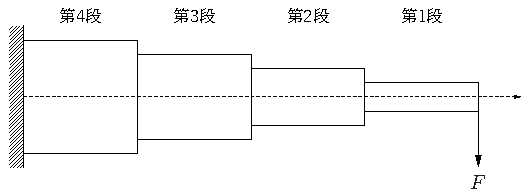
\includegraphics[width=.70\textwidth]{figures/ch04-06.pdf}
\caption*{图4.6\quad 由4段组成的悬臂梁。每段长度为一，截面为矩形。在梁的右端施加竖直力 $F$。}
\end{figure}
设计变量是 $N$ 段的宽度 $w_i$ 和高度 $h_i$。目标是在若干设计约束下最小化梁的总体积，它与重量成正比：
\[
w_1h_1+\cdots+w_Nh_N.
\]
对各段宽度和高度施加上下界
\[
w_{\min}\le w_i\le w_{\max},\quad h_{\min}\le h_i\le h_{\max},\quad i=1,\ldots,N,
\]
并对高宽比施加约束
\[
S_{\min}\le h_i/w_i\le S_{\max}.
\]
此外，对材料最大允许应力和梁端竖直挠度施加限制。

先考虑最大应力约束。第 $i$ 段的最大应力记为 $\sigma_i$，由 $\sigma_i=6iF/(w_ih_i^2)$ 给出。施加约束
\[
\frac{6iF}{w_ih_i^2}\le\sigma_{\max},\quad i=1,\ldots,N,
\]
即可保证梁内任何位置的应力都不超过最大允许值 $\sigma_{\max}$。

最后一个约束限制梁端竖直挠度，记梁端挠度为 $y_1$：
\[
y_1\le y_{\max}.
\]
挠度 $y_1$ 可由涉及各段挠度和斜率的递推求得：
\begin{equation}
\begin{aligned}
v_i&=12(i-1/2)\frac{F}{Ew_ih_i^3}+v_{i+1},\\
y_i&=6(i-1/3)\frac{F}{Ew_ih_i^3}+v_{i+1}+y_{i+1},
\end{aligned}\tag{4.45}
\end{equation}
其中 $i=N,N-1,\ldots,1$，初始值为 $v_{N+1}=y_{N+1}=0$。递推中，$y_i$ 为第 $i$ 段右端的挠度，$v_i$ 为该处斜率。利用（4.45）可以证明，这些挠度和斜率实际上都是变量 $w,h$ 的正项式函数。

% Source PDF page 179 (printed p. 165)
先注意 $v_{N+1}$ 和 $y_{N+1}$ 均为零，因此是正项式。假设 $v_{i+1},y_{i+1}$ 是 $w,h$ 的正项式函数。（4.45）的左式说明，$v_i$ 是一个单项式和正项式 $v_{i+1}$ 之和，因而为正项式。由右式可知，挠度 $y_i$ 是一个单项式及两个正项式 $v_{i+1},y_{i+1}$ 之和，所以也是正项式。特别地，梁端挠度 $y_1$ 是正项式。

于是问题为
\begin{equation}
\begin{array}{ll}
\text{最小化}&\displaystyle\sum_{i=1}^N w_ih_i\\
\text{约束为}&w_{\min}\le w_i\le w_{\max},\quad i=1,\ldots,N,\\
&h_{\min}\le h_i\le h_{\max},\quad i=1,\ldots,N,\\
&S_{\min}\le h_i/w_i\le S_{\max},\quad i=1,\ldots,N,\\
&6iF/(w_ih_i^2)\le\sigma_{\max},\quad i=1,\ldots,N,\\
&y_1\le y_{\max},
\end{array}\tag{4.46}
\end{equation}
变量为 $w,h$。这是GP，因为目标为正项式，全部约束均能写成正项式不等式。（实际上，除挠度上限是复杂的正项式不等式之外，其余约束均可写成单项式不等式。）

分段数 $N$ 很大时，正项式 $y_1$ 中的单项式项数大致按 $N^2$ 增长。习题4.31将研究另一种表述：引入变量 $v_1,\ldots,v_N,y_1,\ldots,y_N$，并用修改后的递推关系作为一组约束。这种表述避免了单项式项数的增长。

\subsubsection*{利用Perron--Frobenius理论最小化谱半径}
设矩阵 $A\in\R^{n\times n}$ 逐元素非负，即 $A_{ij}\ge0$（$i,j=1,\ldots,n$），并且不可约，即矩阵 $(I+A)^{n-1}$ 逐元素为正。Perron--Frobenius定理指出，$A$ 有一个正实特征值 $\lambda_{\mathrm{pf}}$，等于其谱半径，即全部特征值模的最大值。Perron--Frobenius特征值 $\lambda_{\mathrm{pf}}$ 决定 $k\to\infty$ 时 $A^k$ 的渐近增长或衰减速度；事实上，矩阵 $((1/\lambda_{\mathrm{pf}})A)^k$ 收敛。粗略地说，$k\to\infty$ 时，若 $\lambda_{\mathrm{pf}}>1$，$A^k$ 按 $\lambda_{\mathrm{pf}}^k$ 增长；若 $\lambda_{\mathrm{pf}}<1$，则按 $\lambda_{\mathrm{pf}}^k$ 衰减。

非负矩阵理论的一项基本结果为
\[
\lambda_{\mathrm{pf}}=\inf\{\lambda\mid\text{存在 }v\succ0\text{，使 }Av\preceq\lambda v\},
\]
而且下确界能够达到。不等式 $Av\preceq\lambda v$ 可以表示为
\begin{equation}
\sum_{j=1}^n\frac{A_{ij}v_j}{\lambda v_i}\le1,\quad i=1,\ldots,n,\tag{4.47}
\end{equation}
这是一组关于变量 $A_{ij},v_i,\lambda$ 的正项式不等式。因此，条件 $\lambda_{\mathrm{pf}}\le\lambda$ 可表示为关于 $A,v,\lambda$ 的一组正项式不等式。这使得一些涉及Perron--Frobenius特征值的优化问题可以用几何规划求解。

% Source PDF page 180 (printed p. 166)
假设矩阵 $A$ 的元素是某个底层变量 $x\in\R^k$ 的正项式函数。此时不等式（4.47）是关于变量 $x\in\R^k,v\in\R^n,\lambda\in\R$ 的正项式不等式。考虑选择 $x$ 以最小化 $A$ 的Perron--Frobenius特征值或谱半径，并可对 $x$ 施加正项式不等式约束：
\[
\begin{array}{ll}\text{最小化}&\lambda_{\mathrm{pf}}(A(x))\\\text{约束为}&f_i(x)\le1,\quad i=1,\ldots,p,\end{array}
\]
其中 $f_i$ 为正项式。利用上述刻画，可将问题表示为GP
\[
\begin{array}{ll}\text{最小化}&\lambda\\\text{约束为}&\displaystyle\sum_{j=1}^n A_{ij}v_j/(\lambda v_i)\le1,\quad i=1,\ldots,n,\\&f_i(x)\le1,\quad i=1,\ldots,p,\end{array}
\]
变量为 $x,v,\lambda$。

作为具体例子，考虑一种细菌种群动态的简单模型，以 $t=0,1,2,\ldots$ 表示时间或时期，单位为小时。向量 $p(t)\in\R_+^4$ 描述第 $t$ 期的种群年龄分布：$p_1(t)$ 为年龄在0至1小时之间的细菌总数，$p_2(t)$ 为年龄在1至2小时之间的细菌总数，其余类推。我们任意假设细菌寿命不超过4小时。种群随时间按 $p(t+1)=Ap(t)$ 演化，其中
\[
A=\begin{bmatrix}b_1&b_2&b_3&b_4\\s_1&0&0&0\\0&s_2&0&0\\0&0&s_3&0\end{bmatrix}.
\]
这里 $b_i$ 为第 $i$ 年龄组的繁殖率，$s_i$ 为由第 $i$ 年龄组存活至第 $i+1$ 年龄组的比例。假设 $b_i>0$、$0<s_i<1$，从而矩阵 $A$ 不可约。

$A$ 的Perron--Frobenius特征值决定种群的渐近增长或衰减速度。若 $\lambda_{\mathrm{pf}}<1$，种群按 $\lambda_{\mathrm{pf}}^t$ 衰减至零，因此半衰期为 $-1/\log_2\lambda_{\mathrm{pf}}$ 小时。若 $\lambda_{\mathrm{pf}}>1$，种群按 $\lambda_{\mathrm{pf}}^t$ 几何增长，倍增时间为 $1/\log_2\lambda_{\mathrm{pf}}$ 小时。最小化 $A$ 的谱半径，对应寻找种群最快的衰减速度或最慢的增长速度。

作为矩阵 $A$ 所依赖的底层变量，取环境中影响细菌繁殖率和存活率的两种化学物质浓度 $c_1,c_2$。将繁殖率和存活率建模为两种浓度的单项式函数：
\[
\begin{aligned}
b_i&=b_i^{\mathrm{nom}}(c_1/c_1^{\mathrm{nom}})^{\alpha_i}(c_2/c_2^{\mathrm{nom}})^{\beta_i},\quad i=1,\ldots,4,\\
s_i&=s_i^{\mathrm{nom}}(c_1/c_1^{\mathrm{nom}})^{\gamma_i}(c_2/c_2^{\mathrm{nom}})^{\delta_i},\quad i=1,\ldots,3.
\end{aligned}
\]
这里 $b_i^{\mathrm{nom}}$ 为标称繁殖率，$s_i^{\mathrm{nom}}$ 为标称存活率，$c_i^{\mathrm{nom}}$ 为第 $i$ 种化学物质的标称浓度。常数 $\alpha_i,\beta_i,\gamma_i,\delta_i$ 给出化学物质浓度偏离标称值时对繁殖率和存活率的影响。

% Source PDF page 181 (printed p. 167)
例如，$\alpha_2=-0.3$、$\gamma_1=0.5$ 意味着：化学物质1的浓度高于标称浓度时，年龄在1至2小时之间的细菌繁殖率下降，而年龄在0至1小时之间的细菌存活率上升。

假设可以通过给药，独立提高或降低浓度 $c_1,c_2$，例如在标称值的二倍范围内调整。问题是寻找使种群衰减最快，即使 $\lambda_{\mathrm{pf}}(A)$ 最小的药物组合。利用上述方法，可表述为GP
\[
\begin{array}{ll}
\text{最小化}&\lambda\\
\text{约束为}&b_1v_1+b_2v_2+b_3v_3+b_4v_4\le\lambda v_1,\\
&s_1v_1\le\lambda v_2,\\&s_2v_2\le\lambda v_3,\\&s_3v_3\le\lambda v_4,\\
&1/2\le c_i/c_i^{\mathrm{nom}}\le2,\quad i=1,2,\\
&b_i=b_i^{\mathrm{nom}}(c_1/c_1^{\mathrm{nom}})^{\alpha_i}(c_2/c_2^{\mathrm{nom}})^{\beta_i},\quad i=1,\ldots,4,\\
&s_i=s_i^{\mathrm{nom}}(c_1/c_1^{\mathrm{nom}})^{\gamma_i}(c_2/c_2^{\mathrm{nom}})^{\delta_i},\quad i=1,\ldots,3,
\end{array}
\]
变量为 $b_i,s_i,c_i,v_i,\lambda$。

\section{广义不等式约束}
标准形式凸优化问题（4.15）的一个很有用的推广，是允许不等式约束函数取向量值，并在约束中使用广义不等式：
\begin{equation}
\begin{array}{ll}\text{最小化}&f_0(x)\\\text{约束为}&f_i(x)\preceq_{K_i}0,\quad i=1,\ldots,m,\\&Ax=b,\end{array}\tag{4.48}
\end{equation}
其中 $f_0:\R^n\to\R$，$K_i\subseteq\R^{k_i}$ 为正常锥，$f_i:\R^n\to\R^{k_i}$ 为 $K_i$-凸函数。我们称其为具有广义不等式约束的标准形式凸优化问题。问题（4.15）是其中 $K_i=\R_+$（$i=1,\ldots,m$）的特例。

普通凸优化问题的许多结果对广义不等式问题仍然成立，例如：
\begin{itemize}
\item 可行集、任意下水平集和最优集均为凸集；
\item 问题（4.48）的任意局部最优点均为全局最优点；
\item §4.2.3给出的可微 $f_0$ 的最优性条件完全不变，仍然成立。
\end{itemize}
第11章还将看到，带广义不等式约束的凸优化问题通常可以像普通凸优化问题一样容易地求解。

% Source PDF page 182 (printed p. 168)
\subsection{锥形式问题}
带广义不等式的最简单凸优化问题之一，是锥形式问题，或称锥规划。其目标线性，只有一个不等式约束函数，并且该函数仿射，因而 $K$-凸：
\begin{equation}
\begin{array}{ll}\text{最小化}&c^\T x\\\text{约束为}&Fx+g\preceq_K0,\\&Ax=b.\end{array}\tag{4.49}
\end{equation}
当 $K$ 为非负正交象限时，锥形式问题退化为线性规划。因此，可将锥形式问题看作线性规划的推广，以广义线性不等式替换逐分量不等式。

继续类比线性规划，称
\[
\begin{array}{ll}\text{最小化}&c^\T x\\\text{约束为}&x\succeq_K0,\\&Ax=b\end{array}
\]
为标准形式的锥形式问题。类似地，称
\[
\begin{array}{ll}\text{最小化}&c^\T x\\\text{约束为}&Fx+g\preceq_K0\end{array}
\]
为不等式形式的锥形式问题。

\subsection{半正定规划}
当 $K$ 为 $k\times k$ 半正定矩阵构成的锥 $\mathbf S_+^k$ 时，相应锥形式问题称为半正定规划（SDP），形式为
\begin{equation}
\begin{array}{ll}\text{最小化}&c^\T x\\\text{约束为}&x_1F_1+\cdots+x_nF_n+G\preceq0,\\&Ax=b,\end{array}\tag{4.50}
\end{equation}
其中 $G,F_1,\ldots,F_n\in\mathbf S^k$，$A\in\R^{p\times n}$。这里的不等式是线性矩阵不等式，见例2.10。

若 $G,F_1,\ldots,F_n$ 全为对角矩阵，则（4.50）中的LMI等价于一组 $n$ 个线性不等式，SDP（4.50）就退化为线性规划。

\subsubsection*{标准形式与不等式形式的半正定规划}
类比LP，标准形式SDP具有线性等式约束，以及对变量 $X\in\mathbf S^n$ 的矩阵非负约束：
\begin{equation}
\begin{array}{ll}\text{最小化}&\tr(CX)\\\text{约束为}&\tr(A_iX)=b_i,\quad i=1,\ldots,p,\\&X\succeq0,\end{array}\tag{4.51}
\end{equation}

% Source PDF page 183 (printed p. 169)
其中 $C,A_1,\ldots,A_p\in\mathbf S^n$。（回顾 $\tr(CX)=\sum_{i,j=1}^n C_{ij}X_{ij}$ 是 $\mathbf S^n$ 上一般实值线性函数的形式。）可将它与标准形式线性规划（4.28）比较。在LP和SDP的标准形式中，都是在对变量施加 $p$ 个线性等式约束和一个非负约束的条件下，最小化变量的线性函数。

不等式形式SDP与不等式形式LP（4.29）对应，没有等式约束，只有一个LMI：
\[
\begin{array}{ll}\text{最小化}&c^\T x\\\text{约束为}&x_1A_1+\cdots+x_nA_n\preceq B,\end{array}
\]
变量为 $x\in\R^n$，参数为 $B,A_1,\ldots,A_n\in\mathbf S^k$、$c\in\R^n$。

\subsubsection*{多个LMI及线性不等式}
通常也将具有线性目标、线性等式与不等式约束，以及多个LMI约束的问题称为SDP，即
\[
\begin{array}{ll}
\text{最小化}&c^\T x\\
\text{约束为}&F^{(i)}(x)=x_1F_1^{(i)}+\cdots+x_nF_n^{(i)}+G^{(i)}\preceq0,\quad i=1,\ldots,K,\\
&Gx\preceq h,\quad Ax=b.
\end{array}
\]
将各个LMI和线性不等式组成一个大的块对角LMI，就容易变为SDP：
\[
\begin{array}{ll}\text{最小化}&c^\T x\\\text{约束为}&\diag(Gx-h,F^{(1)}(x),\ldots,F^{(K)}(x))\preceq0,\\&Ax=b.\end{array}
\]

\subsection{例子}
\subsubsection*{二阶锥规划}
SOCP（4.36）可表示为锥形式问题
\[
\begin{array}{ll}\text{最小化}&c^\T x\\\text{约束为}&-(A_ix+b_i,c_i^\T x+d_i)\preceq_{K_i}0,\quad i=1,\ldots,m,\\&Fx=g,\end{array}
\]
其中
\[
K_i=\{(y,t)\in\R^{n_i+1}\mid\norm{y}_2\le t\},
\]
即 $\R^{n_i+1}$ 的二阶锥。这就解释了优化问题（4.36）为何称为二阶锥规划。

\subsubsection*{矩阵范数最小化}
令 $A(x)=A_0+x_1A_1+\cdots+x_nA_n$，其中 $A_i\in\R^{p\times q}$。考虑无约束问题
\[
\text{最小化}\quad\norm{A(x)}_2,
\]

% Source PDF page 184 (printed p. 170)
其中 $\norm{\cdot}_2$ 为谱范数，即最大奇异值，变量为 $x\in\R^n$。由于 $\norm{A(x)}_2$ 是 $x$ 的凸函数，此问题是凸问题。

利用 $\norm{A}_2\le s$ 当且仅当 $A^\T A\preceq s^2I$ 且 $s\ge0$，可以将问题写为
\[
\begin{array}{ll}\text{最小化}&s\\\text{约束为}&A(x)^\T A(x)\preceq sI,\end{array}
\]
变量为 $x,s$。由于函数 $A(x)^\T A(x)-sI$ 关于 $(x,s)$ 矩阵凸，这是具有一个 $q\times q$ 矩阵不等式约束的凸优化问题。

也可以利用下述事实，将问题表述为具有一个 $(p+q)\times(p+q)$ 线性矩阵不等式的问题：
\[
A^\T A\preceq t^2I\text{ 且 }t\ge0
\quad\Longleftrightarrow\quad
\begin{bmatrix}tI&A\\A^\T&tI\end{bmatrix}\succeq0
\]
（见§A.5.5）。这得到以 $x,t$ 为变量的SDP
\[
\begin{array}{ll}\text{最小化}&t\\\text{约束为}&\begin{bmatrix}tI&A(x)\\A(x)^\T&tI\end{bmatrix}\succeq0.\end{array}
\]

\subsubsection*{矩问题}
设 $t$ 是 $\R$ 上的随机变量。期望 $\E t^k$（若存在）称为 $t$ 的分布的幂矩。以下经典结果刻画了矩序列。

若存在 $\R$ 上的概率分布，使 $x_k=\E t^k$（$k=0,\ldots,2n$），则 $x_0=1$，并且
\begin{equation}
H(x_0,\ldots,x_{2n})=
\begin{bmatrix}
x_0&x_1&x_2&\cdots&x_{n-1}&x_n\\
x_1&x_2&x_3&\cdots&x_n&x_{n+1}\\
x_2&x_3&x_4&\cdots&x_{n+1}&x_{n+2}\\
\vdots&\vdots&\vdots&&\vdots&\vdots\\
x_{n-1}&x_n&x_{n+1}&\cdots&x_{2n-2}&x_{2n-1}\\
x_n&x_{n+1}&x_{n+2}&\cdots&x_{2n-1}&x_{2n}
\end{bmatrix}\succeq0.\tag{4.52}
\end{equation}
矩阵 $H$ 称为与 $x_0,\ldots,x_{2n}$ 对应的Hankel矩阵。证明很简单：设 $x_i=\E t^i$（$i=0,\ldots,2n$）为某个分布的矩，$y=(y_0,y_1,\ldots,y_n)\in\R^{n+1}$，则
\[
y^\T H(x_0,\ldots,x_{2n})y
=\sum_{i,j=0}^n y_iy_j\E t^{i+j}
=\E(y_0+y_1t^1+\cdots+y_nt^n)^2\ge0.
\]
以下部分逆命题则不那么显然：若 $x_0=1$ 且 $H(x)\succ0$，则存在 $\R$ 上的概率分布，使 $x_i=\E t^i$（$i=0,\ldots,2n$）。

% Source PDF page 185 (printed p. 171)
证明见习题2.37。现在假设 $x_0=1$、$H(x)\succeq0$，但可能 $H(x)\not\succ0$，即线性矩阵不等式（4.52）成立，但未必严格成立。此时存在 $\R$ 上的一列分布，其矩收敛到 $x$。综上，$x_0,\ldots,x_{2n}$ 是某个 $\R$ 上分布的矩，或是一列分布的矩的极限，这一条件可表示为变量 $x$ 的LMI（4.52），加上线性等式 $x_0=1$。由此可将一些有趣的矩问题表述为SDP。

设 $t$ 为 $\R$ 上的随机变量。虽然不知道它的分布，但知道一些矩的界，即
\[
\underline\mu_k\le\E t^k\le\overline\mu_k,\quad k=1,\ldots,2n,
\]
这包括知道某些矩的精确值这一特例。给定 $t$ 的多项式 $p(t)=c_0+c_1t+\cdots+c_{2n}t^{2n}$，其期望关于各阶矩线性：
\[
\E p(t)=\sum_{i=0}^{2n}c_i\E t^i=\sum_{i=0}^{2n}c_ix_i.
\]
为计算满足给定矩界的全部概率分布中 $\E p(t)$ 的上下界，
\[
\begin{array}{ll}\text{最小化（最大化）}&\E p(t)\\\text{约束为}&\underline\mu_k\le\E t^k\le\overline\mu_k,\quad k=1,\ldots,2n,\end{array}
\]
可以求解SDP
\[
\begin{array}{ll}\text{最小化（最大化）}&c_1x_1+\cdots+c_{2n}x_{2n}\\\text{约束为}&\underline\mu_k\le x_k\le\overline\mu_k,\quad k=1,\ldots,2n,\\&H(1,x_1,\ldots,x_{2n})\succeq0,\end{array}
\]
变量为 $x_1,\ldots,x_{2n}$。这给出全部满足已知矩约束的分布中 $\E p(t)$ 的界。此界是紧的，含义是：存在一列分布，其矩满足给定的矩界，而 $\E p(t)$ 收敛到这些SDP求得的上下界。

\subsubsection*{协方差信息不完整时投资组合风险的界}
再次考虑经典Markowitz投资组合问题的设置，见第155页。有 $n$ 种资产或股票，$x_i$ 表示某一投资时期持有的资产 $i$ 的数量，$p_i$ 表示这一时期内资产 $i$ 的相对价格变化。组合总价值变化为 $p^\T x$。价格变化向量 $p$ 建模为随机向量，均值与协方差为
\[
\bar p=\E p,\qquad\Sigma=\E(p-\bar p)(p-\bar p)^\T.
\]
因此，组合价值变化为随机变量，均值 $\bar p^\T x$、标准差 $\sigma=(x^\T\Sigma x)^{1/2}$。较大损失的风险，即组合价值变化显著低于期望的风险，与标准差 $\sigma$ 直接相关，并随其增大而上升。

% Source PDF page 186 (printed p. 172)
因此，用标准差 $\sigma$ 或方差 $\sigma^2$ 衡量投资组合风险。

经典投资组合优化中，投资组合 $x$ 是变量，在最低平均收益和其他约束下最小化风险；价格变化统计量 $\bar p,\Sigma$ 为已知参数。这里的风险界问题反过来考虑：假设组合 $x$ 已知，但只知道协方差矩阵 $\Sigma$ 的部分信息。例如，知道每个元素的上下界
\[
L_{ij}\le\Sigma_{ij}\le U_{ij},\quad i,j=1,\ldots,n,
\]
其中 $L,U$ 给定。我们要问：在全部与给定界相容的协方差矩阵中，组合的最大风险是多少？定义组合的最坏情形方差为
\[
\sigma_{\mathrm{wc}}^2=\sup\{x^\T\Sigma x\mid L_{ij}\le\Sigma_{ij}\le U_{ij},\ i,j=1,\ldots,n,\ \Sigma\succeq0\}.
\]
这里加入了协方差矩阵当然必须满足的条件 $\Sigma\succeq0$。

可以通过求解SDP
\[
\begin{array}{ll}\text{最大化}&x^\T\Sigma x\\\text{约束为}&L_{ij}\le\Sigma_{ij}\le U_{ij},\quad i,j=1,\ldots,n,\\&\Sigma\succeq0\end{array}
\]
求出 $\sigma_{\mathrm{wc}}$，变量为 $\Sigma\in\mathbf S^n$，参数为 $x,L,U$。最优 $\Sigma$ 是满足元素界的最坏协方差矩阵，这里“最坏”指给定组合 $x$ 下的风险最大。由SDP的最优 $\Sigma$ 很容易构造一个满足给定界且达到最坏情形方差的 $p$ 的分布。例如，取 $p=\bar p+\Sigma^{1/2}v$，其中 $v$ 为任意满足 $\E v=0$、$\E vv^\T=I$ 的随机向量。

显然，对关于 $\Sigma$ 的任意凸先验信息，都可用同样方法确定 $\sigma_{\mathrm{wc}}$。下面列举若干例子。
\begin{itemize}
\item \textbf{某些投资组合的方差已知。}可以有形如
\[
u_k^\T\Sigma u_k=\sigma_k^2
\]
的等式约束，其中 $u_k,\sigma_k$ 已知。这对应知道某些已知组合 $u_k$ 的方差，或能非常准确地估计其方差。
\item \textbf{计入估计误差的影响。}若协方差 $\Sigma$ 从经验数据估计，估计方法会给出估计值 $\widehat\Sigma$，以及置信椭球等反映可靠性的信息。可将其表示为
\[
C(\Sigma-\widehat\Sigma)\le\alpha,
\]
其中 $C$ 是 $\mathbf S^n$ 上的正定二次型，常数 $\alpha$ 决定置信水平。
% Source PDF page 187 (printed p. 173)
\item \textbf{因子模型。}协方差可能形如
\[
\Sigma=F\Sigma_{\mathrm{factor}}F^\T+D,
\]
其中 $F\in\R^{n\times k}$、$\Sigma_{\mathrm{factor}}\in\mathbf S^k$，$D$ 为对角矩阵。这对应价格变化模型
\[
p=Fz+d,
\]
其中 $z$ 为随机变量，表示影响价格变化的底层因子，而 $d_i$ 相互独立，表示各资产价格的额外波动。假设因子已知。由于 $\Sigma$ 与 $\Sigma_{\mathrm{factor}},D$ 之间具有线性关系，可对后两者施加任意反映先验信息的凸约束，仍能用凸优化计算 $\sigma_{\mathrm{wc}}$。
\item \textbf{相关系数信息。}最简单的情形是 $\Sigma$ 的对角元素已知，即各资产价格波动程度已知，并且知道价格变化之间相关系数的界：
\[
l_{ij}\le\rho_{ij}=\frac{\Sigma_{ij}}{\Sigma_{ii}^{1/2}\Sigma_{jj}^{1/2}}\le u_{ij},\quad i,j=1,\ldots,n.
\]
由于 $\Sigma_{ii}$ 已知，而 $i\ne j$ 时的 $\Sigma_{ij}$ 未知，这些是线性不等式。
\end{itemize}

\subsubsection*{图上混合最快的马尔可夫链}
考虑无向图，结点为 $1,\ldots,n$，边集为
\[
\mathcal E\subseteq\{1,\ldots,n\}\times\{1,\ldots,n\}.
\]
$(i,j)\in\mathcal E$ 表示结点 $i,j$ 间有边。由于图无向，$\mathcal E$ 对称，即 $(i,j)\in\mathcal E$ 当且仅当 $(j,i)\in\mathcal E$。允许自环，即可以有 $(i,i)\in\mathcal E$。

定义马尔可夫链，状态为 $X(t)\in\{1,\ldots,n\}$，其中 $t\in\Z_+$，即非负整数。为每条边 $(i,j)\in\mathcal E$ 关联概率 $P_{ij}$，表示 $X$ 在结点 $i,j$ 之间转移的概率。状态只能沿边转移，故 $(i,j)\notin\mathcal E$ 时 $P_{ij}=0$。各边概率非负；对每个结点，与之相连的边的概率之和必须为一，包括存在的自环。

马尔可夫链的转移概率矩阵为
\[
P_{ij}=\Prob(X(t+1)=i\mid X(t)=j),\quad i,j=1,\ldots,n.
\]
矩阵必须满足
\begin{equation}
P_{ij}\ge0,\quad i,j=1,\ldots,n,\qquad\one^\T P=\one^\T,\qquad P=P^\T,\tag{4.53}
\end{equation}
以及
\begin{equation}
P_{ij}=0\quad\text{若 }(i,j)\notin\mathcal E.\tag{4.54}
\end{equation}

% Source PDF page 188 (printed p. 174)
由于 $P$ 对称且 $\one^\T P=\one^\T$，可得 $P\one=\one$，所以均匀分布 $(1/n)\one$ 是此链的平衡分布。$X(t)$ 的分布收敛到 $(1/n)\one$ 的速度由 $P$ 按模排列第二大的特征值决定，即由 $r=\max\{\lambda_2,-\lambda_n\}$ 决定，其中
\[
1=\lambda_1\ge\lambda_2\ge\cdots\ge\lambda_n
\]
为 $P$ 的特征值。称 $r$ 为马尔可夫链的混合率。

若 $r=1$，$X(t)$ 的分布未必收敛到 $(1/n)\one$，即马尔可夫链不混合。当 $r<1$ 时，$t\to\infty$ 时 $X(t)$ 的分布按 $r^t$ 渐近接近 $(1/n)\one$。所以 $r$ 越小，马尔可夫链混合越快。

最快混合马尔可夫链问题，是在约束（4.53）、（4.54）下寻找使 $r$ 最小的 $P$。（问题数据是图，即边集 $\mathcal E$。）下面说明它可表述为SDP。

特征值 $\lambda_1=1$ 对应特征向量 $\one$，所以混合率可表示为 $P$ 在子空间 $\one^\perp$ 上的限制的范数：$r=\norm{QPQ}_2$，其中 $Q=I-(1/n)\one\one^\T$ 表示到 $\one^\perp$ 的正交投影。利用 $P\one=\one$，有
\[
\begin{aligned}
r&=\norm{QPQ}_2\\
&=\norm{(I-(1/n)\one\one^\T)P(I-(1/n)\one\one^\T)}_2\\
&=\norm{P-(1/n)\one\one^\T}_2.
\end{aligned}
\]
这说明混合率 $r$ 为 $P$ 的凸函数，所以最快混合马尔可夫链问题可写成凸优化问题
\[
\begin{array}{ll}\text{最小化}&\norm{P-(1/n)\one\one^\T}_2\\\text{约束为}&P\one=\one,\\&P_{ij}\ge0,\quad i,j=1,\ldots,n,\\&P_{ij}=0\quad\text{若 }(i,j)\notin\mathcal E,\end{array}
\]
变量为 $P\in\mathbf S^n$。引入标量变量 $t$ 对 $P-(1/n)\one\one^\T$ 的范数给出上界，即可表示为SDP：
\begin{equation}
\begin{array}{ll}\text{最小化}&t\\\text{约束为}&-tI\preceq P-(1/n)\one\one^\T\preceq tI,\\&P\one=\one,\\&P_{ij}\ge0,\quad i,j=1,\ldots,n,\\&P_{ij}=0\quad\text{若 }(i,j)\notin\mathcal E.\end{array}\tag{4.55}
\end{equation}

\section{向量优化}
\subsection{一般向量优化问题与凸向量优化问题}
§4.6将标准形式问题（4.1）推广到向量值约束函数。本节研究向量值目标函数的含义。

% Source PDF page 189 (printed p. 175)
一般向量优化问题记为
\begin{equation}
\begin{array}{ll}\text{最小化（关于 }K\text{）}&f_0(x)\\\text{约束为}&f_i(x)\le0,\quad i=1,\ldots,m,\\&h_i(x)=0,\quad i=1,\ldots,p.\end{array}\tag{4.56}
\end{equation}
这里 $x\in\R^n$ 为优化变量，$K\subseteq\R^q$ 为正常锥，$f_0:\R^n\to\R^q$ 为目标函数，$f_i:\R^n\to\R$ 为不等式约束函数，$h_i:\R^n\to\R$ 为等式约束函数。它与标准优化问题（4.1）的唯一区别在于：这里目标取 $\R^q$ 中的值，问题还指定了用于比较目标值的正常锥 $K$。在向量优化的语境下，有时称标准优化问题（4.1）为标量优化问题。

若目标 $f_0$ 为 $K$-凸函数，不等式约束函数 $f_1,\ldots,f_m$ 凸，等式约束函数 $h_1,\ldots,h_p$ 仿射，就称（4.56）为凸向量优化问题。（和标量情形一样，通常将等式约束写为 $Ax=b$，其中 $A\in\R^{p\times n}$。）

怎样理解向量优化问题（4.56）？设 $x,y$ 为两个可行点，即满足全部约束。对应目标值 $f_0(x),f_0(y)$ 要通过广义不等式 $\preceq_K$ 比较。$f_0(x)\preceq_K f_0(y)$ 表示：以目标 $f_0$ 关于 $K$ 衡量时，$x$ 的价值“优于或等于”$y$。向量优化令人困惑之处是，两个目标值 $f_0(x),f_0(y)$ 未必可比；可能既没有 $f_0(x)\preceq_K f_0(y)$，也没有 $f_0(y)\preceq_K f_0(x)$，即谁也不比谁好。标量目标优化中不会出现这种情形。

\subsection{最优点与最优值}
先考虑向量优化问题含义明确的一种特殊情形。可行点的目标值集合
\[
\mathcal O=\{f_0(x)\mid\exists x\in\mathcal D,\ f_i(x)\le0,\ i=1,\ldots,m,\ h_i(x)=0,\ i=1,\ldots,p\}\subseteq\R^q
\]
称为可达目标值集。若该集合有最小元（见§2.4.2），即存在可行点 $x$，使对所有可行点 $y$ 有 $f_0(x)\preceq_K f_0(y)$，就称 $x$ 为问题（4.56）的最优点，称 $f_0(x)$ 为最优值。（向量优化问题若有最优值，则它唯一。）若 $x^\star$ 最优，$f_0(x^\star)$ 就可与其他每个可行点的目标值比较，且优于或等于它。粗略地说，$x^\star$ 是可行点中一个无歧义的最佳选择。

点 $x^\star$ 最优，当且仅当它可行且
\begin{equation}
\mathcal O\subseteq f_0(x^\star)+K\tag{4.57}
\end{equation}

% Source PDF page 190 (printed p. 176)
\begin{figure}[htbp]
\centering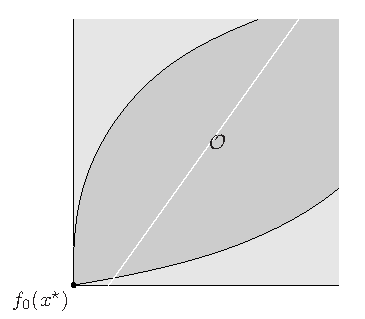
\includegraphics[width=.60\textwidth]{figures/ch04-07.pdf}
\caption*{图4.7\quad 向量优化的可达值集 $\mathcal O$ 为阴影部分，目标值位于 $\R^2$，锥为 $K=\R_+^2$。此时标出的 $f_0(x^\star)$ 是问题的最优值，$x^\star$ 为最优点。目标值 $f_0(x^\star)$ 可与每个其他可达值 $f_0(y)$ 比较，且优于或等于 $f_0(y)$。（这里“优于或等于”指“位于下方和左方”。）浅阴影区域为 $f_0(x^\star)+K$，即对应于比 $f_0(x^\star)$ 更差或与之相等的目标值的所有 $z\in\R^2$ 的集合。}
\end{figure}
（见§2.4.2）。集合 $f_0(x^\star)+K$ 可解释为比 $f_0(x^\star)$ 更差或与之相等的值构成的集合，所以（4.57）表示每个可达值都落在其中。图4.7说明了这一点。大多数向量优化问题没有最优点和最优值，但一些特殊情形中存在。

\begin{origexample}{4.9}
\textbf{最佳线性无偏估计。}设 $y=Ax+v$，其中 $v\in\R^m$ 为测量噪声，$y\in\R^m$ 为测量向量，$x\in\R^n$ 为给定测量 $y$ 后要估计的向量。假设 $A$ 的秩为 $n$，测量噪声满足 $\E v=0$、$\E vv^\T=I$，即其各分量零均值且不相关。

$x$ 的线性估计形如 $\widehat x=Fy$。若对所有 $x$ 有 $\E\widehat x=x$，即 $FA=I$，就称估计无偏。无偏估计的误差协方差为
\[
\E(\widehat x-x)(\widehat x-x)^\T=\E Fvv^\T F^\T=FF^\T.
\]
目标是找一个误差协方差矩阵“较小”的无偏估计。可通过矩阵不等式，即关于 $\mathbf S_+^n$，比较误差协方差。其含义如下：设 $\widehat x_1=F_1y$、$\widehat x_2=F_2y$ 为两个无偏估计。第一个估计至少与第二个一样好，即 $F_1F_1^\T\preceq F_2F_2^\T$，当且仅当对所有 $c$，有
\[
\E(c^\T\widehat x_1-c^\T x)^2\le\E(c^\T\widehat x_2-c^\T x)^2.
\]
换言之，对 $x$ 的任意线性函数，$F_1$ 给出的估计至少与 $F_2$ 一样好。

% Source PDF page 191 (printed p. 177)
寻找 $x$ 的无偏估计的问题，可以表述为向量优化问题
\begin{equation}
\begin{array}{ll}\text{最小化（关于 }\mathbf S_+^n\text{）}&FF^\T\\\text{约束为}&FA=I,\end{array}\tag{4.58}
\end{equation}
变量为 $F\in\R^{n\times m}$。目标 $FF^\T$ 关于 $\mathbf S_+^n$ 凸，所以（4.58）是凸向量优化问题。一个简单证明是：对任意固定 $v$，$v^\T FF^\T v=\norm{F^\T v}_2^2$ 是 $F$ 的凸函数。

一个著名结果指出，（4.58）有最优解，即最小二乘估计或伪逆
\[
F^\star=A^\dagger=(A^\T A)^{-1}A^\T.
\]
对任意满足 $FA=I$ 的 $F$，有 $FF^\T\succeq F^\star F^{\star\T}$。矩阵
\[
F^\star F^{\star\T}=A^\dagger A^{\dagger\T}=(A^\T A)^{-1}
\]
是问题（4.58）的最优值。
\end{origexample}

\subsection{Pareto最优点与最优值}
现在考虑可达目标值集没有最小元的情形，这也是大多数有意义的向量优化问题的情况；此时问题没有最优点或最优值。可达值集的极小元在这些情形中起重要作用。若 $f_0(x)$ 是可达值集 $\mathcal O$ 的极小元，就称可行点 $x$ 为Pareto最优点，或有效点。此时称 $f_0(x)$ 为向量优化问题（4.56）的Pareto最优值。因此，$x$ 为Pareto最优点，意味着它可行，且对任意可行点 $y$，$f_0(y)\preceq_K f_0(x)$ 蕴含 $f_0(y)=f_0(x)$。换言之，任意优于或等于 $x$ 的可行点 $y$，即满足 $f_0(y)\preceq_K f_0(x)$ 的点，其目标值必与 $x$ 完全相同。

点 $x$ 为Pareto最优点，当且仅当它可行且
\begin{equation}
(f_0(x)-K)\cap\mathcal O=\{f_0(x)\}\tag{4.59}
\end{equation}
（见§2.4.2）。集合 $f_0(x)-K$ 可解释为优于或等于 $f_0(x)$ 的值组成的集合，因此（4.59）表示：优于或等于 $f_0(x)$ 的可达值只有 $f_0(x)$ 本身。图4.8说明了这一点。

向量优化问题可以有多个Pareto最优值和最优点。Pareto最优值的集合记为 $\mathcal P$，满足
\[
\mathcal P\subseteq\mathcal O\cap\operatorname{bd}\mathcal O,
\]
即每个Pareto最优值都是位于可达目标值集边界上的可达目标值，见习题4.52。

% Source PDF page 192 (printed p. 178)
\begin{figure}[htbp]
\centering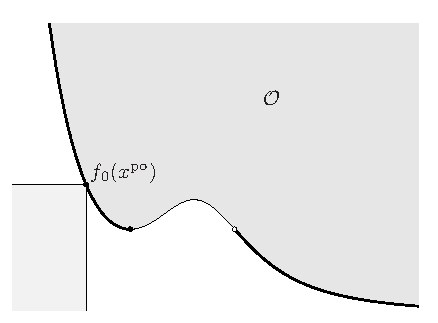
\includegraphics[width=.60\textwidth]{figures/ch04-08.pdf}
\caption*{图4.8\quad 向量优化的可达值集 $\mathcal O$ 为阴影部分，目标值位于 $\R^2$，锥为 $K=\R_+^2$。问题没有最优点或最优值，但有一组Pareto最优点，对应的值以 $\mathcal O$ 左下边界的粗曲线表示。标出的 $f_0(x^{\mathrm{po}})$ 是Pareto最优值，$x^{\mathrm{po}}$ 是Pareto最优点。浅阴影区域为 $f_0(x^{\mathrm{po}})-K$，即与优于或等于 $f_0(x^{\mathrm{po}})$ 的目标值对应的全部 $z\in\R^2$。}
\end{figure}

\subsection{标量化}
标量化是寻找向量优化问题的Pareto最优点或最优点的一种标准技巧，基于§2.6.3通过对偶广义不等式对最小元和极小元的刻画。任取 $\lambda\succ_{K^*}0$，即一个在对偶广义不等式下为正的向量。考虑标量优化问题
\begin{equation}
\begin{array}{ll}\text{最小化}&\lambda^\T f_0(x)\\\text{约束为}&f_i(x)\le0,\quad i=1,\ldots,m,\\&h_i(x)=0,\quad i=1,\ldots,p,\end{array}\tag{4.60}
\end{equation}
设 $x$ 为其最优点，则 $x$ 是向量优化问题（4.56）的Pareto最优点。这可由§2.6.3的极小元的对偶不等式刻画得到，也容易直接证明。若 $x$ 不是Pareto最优点，则存在可行 $y$ 满足 $f_0(y)\preceq_K f_0(x)$，且 $f_0(x)\ne f_0(y)$。由于 $f_0(x)-f_0(y)\succeq_K0$ 且非零，有 $\lambda^\T(f_0(x)-f_0(y))>0$，即 $\lambda^\T f_0(x)>\lambda^\T f_0(y)$，与 $x$ 为标量问题（4.60）的最优点矛盾。

借助标量化，可以通过求解普通标量优化问题（4.60），寻找任意向量优化问题的Pareto最优点。向量 $\lambda$ 有时称为权重向量，必须满足 $\lambda\succ_{K^*}0$。权重向量是自由参数；改变它，可能得到向量优化问题（4.56）的不同Pareto最优解，见图4.9。图中还给出一个Pareto最优点：对于任何权重 $\lambda\succ_{K^*}0$，它都不能由标量化得到。

% Source PDF page 193 (printed p. 179)
\begin{figure}[htbp]
\centering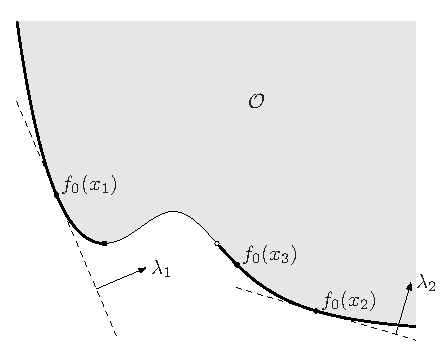
\includegraphics[width=.60\textwidth]{figures/ch04-09.pdf}
\caption*{图4.9\quad 标量化。向量优化问题的可达值集为 $\mathcal O$，锥为 $K=\R_+^2$。图中标出三个Pareto最优值 $f_0(x_1),f_0(x_2),f_0(x_3)$。前两个值可由标量化得到：$f_0(x_1)$ 在全部 $u\in\mathcal O$ 中最小化 $\lambda_1^\T u$，$f_0(x_2)$ 最小化 $\lambda_2^\T u$，其中 $\lambda_1,\lambda_2\succ0$。$f_0(x_3)$ 虽为Pareto最优值，却不能通过标量化得到。}
\end{figure}
标量化也有几何解释。点 $x$ 为标量化问题最优点，即在可行集上最小化 $\lambda^\T f_0$，当且仅当对所有可行 $y$，有 $\lambda^\T(f_0(y)-f_0(x))\ge0$。这等价于说，$\{u\mid-\lambda^\T(u-f_0(x))=0\}$ 在点 $f_0(x)$ 处是可达目标值集 $\mathcal O$ 的支撑超平面；特别地，
\begin{equation}
\{u\mid\lambda^\T(u-f_0(x))<0\}\cap\mathcal O=\varnothing.\tag{4.61}
\end{equation}
见图4.9。因此，求得标量化问题的最优点时，不仅得到原向量优化问题的一个Pareto最优点，还得到 $\R^q$ 中由（4.61）给出的整个半空间，其中目标值均不可达。

\subsubsection*{凸向量优化问题的标量化}
现在假设向量优化问题（4.56）凸，则标量化问题（4.60）也凸，因为由§3.6，$\lambda^\T f_0$ 是标量值凸函数。这意味着，可以通过求解凸标量优化问题，寻找凸向量优化问题的Pareto最优点。每选一个 $\lambda\succ_{K^*}0$，就得到一个通常不同的Pareto最优点。

对凸向量优化问题，有一个部分逆命题：每个Pareto最优点 $x^{\mathrm{po}}$ 都对应某个非零 $\lambda\succeq_{K^*}0$，使 $x^{\mathrm{po}}$ 是标量化问题（4.60）的解。粗略地说，对凸问题，让权重向量 $\lambda$ 遍历关于 $K^*$ 非负且非零的取值，标量化就会产生全部Pareto最优点。

% Source PDF page 194 (printed p. 180)
这里需要谨慎，因为 $\lambda\succeq_{K^*}0$、$\lambda\ne0$ 时，标量化问题并非每个解都是向量问题的Pareto最优点。相比之下，$\lambda\succ_{K^*}0$ 时，每个解都是Pareto最优点。

有时可以利用这一部分逆命题找到凸向量优化问题的全部Pareto最优点。取 $\lambda\succ_{K^*}0$ 标量化，可以得到一组Pareto最优点，这在非凸向量优化中同样成立。为找出其余Pareto最优解，还需考虑满足 $\lambda\succeq_{K^*}0$ 的非零权重。对每个这样的权重，先找出标量化问题的全部解，再检查其中哪些确实对向量问题Pareto最优。这些“极端”的Pareto最优点，也可由正权重产生的Pareto最优点取极限得到。

为证明这一部分逆命题，考虑集合
\begin{equation}
\mathcal A=\mathcal O+K=\{t\in\R^q\mid\text{存在可行 }x\text{，使 }f_0(x)\preceq_K t\},\tag{4.62}
\end{equation}
它由比某个可达目标值更差或与之相等的值组成，这里按 $\preceq_K$ 比较。虽然可达目标值集 $\mathcal O$ 未必凸，问题凸时 $\mathcal A$ 却为凸集。而且，$\mathcal A$ 的极小元恰与可达值集 $\mathcal O$ 的极小元相同，也就是Pareto最优值，见习题4.53。由§2.6.3可知，$\mathcal A$ 的任意极小元都对某个非零 $\lambda\succeq_{K^*}0$ 在 $\mathcal A$ 上最小化 $\lambda^\T z$。这意味着，每个向量问题的Pareto最优点，都对某个非零权重 $\lambda\succeq_{K^*}0$ 是标量化问题的最优点。

\begin{origexample}{4.10}
\textbf{一组矩阵的极小上界。}考虑关于半正定锥的凸向量优化问题
\begin{equation}
\begin{array}{ll}\text{最小化（关于 }\mathbf S_+^n\text{）}&X\\\text{约束为}&X\succeq A_i,\quad i=1,\ldots,m,\end{array}\tag{4.63}
\end{equation}
其中 $A_i\in\mathbf S^n$（$i=1,\ldots,m$）已知。约束表示 $X$ 是给定矩阵 $A_1,\ldots,A_m$ 的上界；（4.63）的Pareto最优解就是这些矩阵的一个极小上界。

为求Pareto最优点，应用标量化：任选 $W\in\mathbf S_{++}^n$，形成问题
\begin{equation}
\begin{array}{ll}\text{最小化}&\tr(WX)\\\text{约束为}&X\succeq A_i,\quad i=1,\ldots,m,\end{array}\tag{4.64}
\end{equation}
这是SDP。一般而言，不同 $W$ 会给出不同的极小解。

部分逆命题表明，若 $X$ 对向量问题（4.63）Pareto最优，则对某个非零权重矩阵 $W\succeq0$，它是SDP（4.64）的最优点。（但此时（4.64）的解并非全都对向量问题Pareto最优。）

这个问题有简单的几何解释。为每个 $A\in\mathbf S_{++}^n$ 关联一个以原点为中心的椭球
\[
\mathcal E_A=\{u\mid u^\T A^{-1}u\le1\},
\]

% Source PDF page 195 (printed p. 181)
\begin{figure}[htbp]
\centering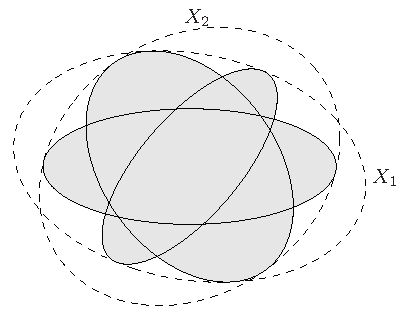
\includegraphics[width=.55\textwidth]{figures/ch04-10.pdf}
\caption*{图4.10\quad 问题（4.63）的几何解释。三个阴影椭球对应数据 $A_1,A_2,A_3\in\mathbf S_{++}^2$；Pareto最优点对应包含它们的极小椭球。边界标为 $X_1,X_2$ 的两个椭球，是用不同权重矩阵 $W_1,W_2$ 求解SDP（4.64）所得的两个极小椭球。}
\end{figure}
于是 $A\preceq B$ 当且仅当 $\mathcal E_A\subseteq\mathcal E_B$。问题（4.63）的Pareto最优点 $X$，对应一个包含与 $A_1,\ldots,A_m$ 关联椭球的极小椭球。图4.10给出一例。
\end{origexample}

\subsection{多准则优化}
向量优化问题的锥为 $K=\R_+^q$ 时，称为多准则或多目标优化问题。$f_0$ 的分量记为 $F_1,\ldots,F_q$，可解释为 $q$ 个不同的标量目标，我们希望每一个都尽可能小。称 $F_i$ 为问题的第 $i$ 个目标。多准则问题凸，要求 $f_1,\ldots,f_m$ 凸、$h_1,\ldots,h_p$ 仿射，并且目标 $F_1,\ldots,F_q$ 均凸。

多准则问题是向量优化问题，所以§4.7.1至§4.7.4的全部内容都适用。不过，多准则问题的解释可以更具体。对可行点 $x$，可将 $F_i(x)$ 看作按第 $i$ 个目标评定的得分或价值。若 $x,y$ 均可行，$F_i(x)\le F_i(y)$ 表示按第 $i$ 个目标 $x$ 至少与 $y$ 一样好；$F_i(x)<F_i(y)$ 表示按第 $i$ 个目标 $x$ 优于或胜过 $y$。若 $x,y$ 均可行，且 $F_i(x)\le F_i(y)$（$i=1,\ldots,q$），并至少存在一个 $j$ 使 $F_j(x)<F_j(y)$，就称 $x$ 优于或支配 $y$。粗略地说，$x$ 在所有目标上都不逊于 $y$，并至少在一个目标上胜过 $y$，就称 $x$ 更好。

多准则问题的最优点 $x^\star$ 满足，对每个可行 $y$，
\[
F_i(x^\star)\le F_i(y),\quad i=1,\ldots,q.
\]

% Source PDF page 196 (printed p. 182)
换言之，对 $j=1,\ldots,q$，$x^\star$ 同时是各个标量问题
\[
\begin{array}{ll}\text{最小化}&F_j(x)\\\text{约束为}&f_i(x)\le0,\quad i=1,\ldots,m,\\&h_i(x)=0,\quad i=1,\ldots,p\end{array}
\]
的最优点。存在最优点时，称各目标不竞争，因为无需在目标之间妥协：每个目标都达到即使忽略其他目标也只能达到的最小值。

Pareto最优点 $x^{\mathrm{po}}$ 满足：若 $y$ 可行，且 $F_i(y)\le F_i(x^{\mathrm{po}})$（$i=1,\ldots,q$），则 $F_i(x^{\mathrm{po}})=F_i(y)$（$i=1,\ldots,q$）。也就是说，一个点Pareto最优，当且仅当它可行且不存在更好的可行点。特别地，若可行点不Pareto最优，则至少存在另一个更好的可行点。因此寻找好的点时，显然只需搜索Pareto最优点。

\subsubsection*{权衡分析}
设 $x,y$ 为Pareto最优点，例如
\[
\begin{aligned}
F_i(x)&<F_i(y),&&i\in\mathcal A,\\
F_i(x)&=F_i(y),&&i\in\mathcal B,\\
F_i(x)&>F_i(y),&&i\in\mathcal C,
\end{aligned}
\]
其中 $\mathcal A\cup\mathcal B\cup\mathcal C=\{1,\ldots,q\}$。换言之，$\mathcal A$ 是 $x$ 胜过 $y$ 的目标指标集，$\mathcal B$ 是两点打平的目标集，$\mathcal C$ 是 $y$ 胜过 $x$ 的目标集。若 $\mathcal A,\mathcal C$ 均为空，两点的全部目标值相同；否则两者都必须非空。因此，比较两个Pareto最优点时，要么两者性能相同，即全部目标相等；要么各自至少在一个目标上胜过对方。

比较 $x$ 与 $y$ 时，可以说我们用 $i\in\mathcal C$ 的较差目标值，换取了 $i\in\mathcal A$ 的较好目标值。最优权衡分析，或简称权衡分析，研究为了改善某些目标，必须让另一个或多个目标变差多少；更一般地，它研究哪些目标值组合可达。

例如，考虑双准则问题。设 $x$ 为Pareto最优点，目标值为 $F_1(x),F_2(x)$。我们可以问：为了找到满足 $F_1(z)\le F_1(x)-a$ 的可行点 $z$，$F_2(z)$ 必须增大多少，其中 $a>0$ 为常数。粗略地说，这是问为了让第一个目标改善 $a$，必须在第二个目标上支付多少代价。若 $F_1$ 的小幅下降需要接受 $F_2$ 的大幅上升，就说在Pareto最优值 $(F_1(x),F_2(x))$ 附近，两目标之间的权衡很强。反之，若 $F_2$ 只需小幅上升即可让 $F_1$ 大幅下降，就说附近的权衡很弱。

也可以考虑以第一个目标的较差性能，换取第二个目标的改善。这时要在 $F_1(z)\le F_1(x)+a$ 的条件下，考察 $F_2(z)$ 可以降低多少，其中 $a>0$。

% Source PDF page 197 (printed p. 183)
此时获得的第二目标收益，就是 $F_2$ 相对于 $F_2(x)$ 的下降。若收益很大，即 $F_1$ 小幅增加换得 $F_2$ 大幅下降，就说目标之间权衡很强；若收益很小，就说在Pareto最优值 $(F_1(x),F_2(x))$ 附近权衡很弱。

\subsubsection*{最优权衡曲面}
多准则问题的Pareto最优值集，通常在 $q>2$ 时称为最优权衡曲面，在 $q=2$ 时称为最优权衡曲线。（接受一个非Pareto最优点是不明智的，因此权衡分析可以限于Pareto最优点。）权衡分析有时也称为探索最优权衡曲面。（最优权衡曲面通常、但并非总是通常意义下的曲面。例如，问题有最优点时，最优权衡曲面只包含最优值这一个点。）

最优权衡曲线很容易解释。第185页图4.11给出凸双准则问题的一例。由曲线可以直观理解两目标的权衡。
\begin{itemize}
\item 右端点给出完全不考虑 $F_1$ 时，$F_2$ 的最小可能值。
\item 左端点给出完全不考虑 $F_2$ 时，$F_1$ 的最小可能值。
\item 找曲线与竖线 $F_1=\alpha$ 的交点，可知为达到 $F_1\le\alpha$，$F_2$ 必须多大。
\item 找曲线与横线 $F_2=\beta$ 的交点，可知为达到 $F_2\le\beta$，$F_1$ 必须多大。
\item 曲线上某点，即某个Pareto最优值处的斜率，反映两目标的局部最优权衡。斜率陡峭处，$F_1$ 的小变化伴随 $F_2$ 的大变化。
\item 曲率大的点，是一个目标的小幅下降只能通过另一个目标的大幅增加实现的位置。这就是常说的权衡曲线“膝点”，在许多应用中代表良好的折中解。
\end{itemize}
这些解释都容易推广到权衡曲面，不过超过三个目标的曲面难以可视化。

\subsubsection*{多准则问题的标量化}
通过加权和目标
\[
\lambda^\T f_0(x)=\sum_{i=1}^q\lambda_iF_i(x),\qquad\lambda\succ0
\]
对多准则问题进行标量化时，可以将 $\lambda_i$ 解释为赋予第 $i$ 个目标的权重。

% Source PDF page 198 (printed p. 184)
权重 $\lambda_i$ 可看作衡量希望 $F_i$ 较小的程度，或反对 $F_i$ 较大的程度。特别地，若希望 $F_i$ 小，应取较大的 $\lambda_i$；若对 $F_i$ 的关心小得多，可取较小的 $\lambda_i$。比值 $\lambda_i/\lambda_j$ 可解释为第 $i$ 个目标相对于第 $j$ 个的权重或重要性。也可将它看作两目标的兑换率，因为在加权目标中，$F_i$ 下降 $\alpha$，等同于 $F_j$ 上升 $(\lambda_i/\lambda_j)\alpha$。

这些解释为探索最优权衡曲面时设置和调整权重提供直觉。例如，权重向量 $\lambda\succ0$ 得到Pareto最优点 $x^{\mathrm{po}}$，目标值为 $F_1(x^{\mathrm{po}}),\ldots,F_q(x^{\mathrm{po}})$。为寻找可能的新Pareto最优点，让第 $k$ 个目标改善，而其他目标可能变差，构造新权重向量 $\widetilde\lambda$，满足
\[
\widetilde\lambda_k>\lambda_k,\qquad\widetilde\lambda_j=\lambda_j,\quad j\ne k,\quad j=1,\ldots,q,
\]
即增大第 $k$ 个目标的权重。得到的新Pareto最优点 $\widetilde x^{\mathrm{po}}$ 满足 $F_k(\widetilde x^{\mathrm{po}})\le F_k(x^{\mathrm{po}})$，通常为严格小于，即第 $k$ 个目标改善。

还可看到，在最优权衡曲面光滑的任意一点，$\lambda$ 是相应Pareto最优点处指向曲面内部的法向量。特别地，选择权重向量 $\lambda$ 并标量化，得到的Pareto最优点处，$\lambda$ 给出了目标间的局部权衡。

实际中，常依据上述直觉，逐次试调权重来探索最优权衡曲面。第5章将看到，标量化的基本思想，即最小化目标的加权和，再调整权重得到合适解，正是对偶性的核心。

\subsection{例子}
\subsubsection*{正则化最小二乘}
给定 $A\in\R^{m\times n}$、$b\in\R^m$，希望选择 $x\in\R^n$，同时考虑两个二次目标：
\begin{itemize}
\item $F_1(x)=\norm{Ax-b}_2^2=x^\T A^\T Ax-2b^\T Ax+b^\T b$，衡量 $Ax$ 与 $b$ 的不匹配程度；
\item $F_2(x)=\norm{x}_2^2=x^\T x$，衡量 $x$ 的大小。
\end{itemize}
目标是寻找拟合较好，即 $F_1$ 小，同时幅度不大，即 $F_2$ 小的 $x$。可将其写成关于锥 $\R_+^2$ 的向量优化问题，即无约束双准则问题：
\[
\text{最小化（关于 }\R_+^2\text{）}\quad f_0(x)=(F_1(x),F_2(x)).
\]

% Source PDF page 199 (printed p. 185)
\begin{figure}[htbp]
\centering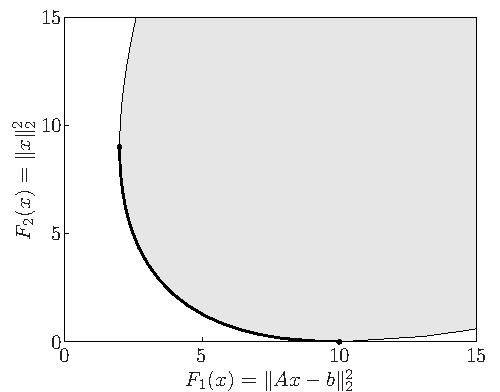
\includegraphics[width=.65\textwidth]{figures/ch04-11.pdf}
\caption*{图4.11\quad 正则化最小二乘问题的最优权衡曲线。阴影区域为可达值 $(\norm{Ax-b}_2^2,\norm{x}_2^2)$ 的集合。加粗的最优权衡曲线是边界的左下部分。}
\end{figure}
取 $\lambda_1>0$、$\lambda_2>0$，最小化标量加权目标，就可将问题标量化：
\[
\begin{aligned}
\lambda^\T f_0(x)&=\lambda_1F_1(x)+\lambda_2F_2(x)\\
&=x^\T(\lambda_1A^\T A+\lambda_2I)x-2\lambda_1b^\T Ax+\lambda_1b^\T b,
\end{aligned}
\]
从而得到
\[
x(\mu)=(\lambda_1A^\T A+\lambda_2I)^{-1}\lambda_1A^\T b
=(A^\T A+\mu I)^{-1}A^\T b,
\]
其中 $\mu=\lambda_2/\lambda_1$。对任意 $\mu>0$，此点都对双准则问题Pareto最优。$\mu$ 可解释为赋予 $F_2$ 相对于 $F_1$ 的权重。

这种方法能得到全部Pareto最优点，唯独缺少对应极端情形 $\mu\to\infty$ 与 $\mu\to0$ 的两个点。第一种情形的Pareto最优解为 $x=0$，可用 $\lambda=(0,1)$ 标量化得到。另一端的Pareto最优解为 $A^\dagger b$，其中 $A^\dagger$ 为 $A$ 的伪逆。它可作为 $\mu\to0$，即 $\lambda\to(1,0)$ 时标量化问题最优解的极限得到。（§6.3.2还会讨论正则化最小二乘。）

图4.11展示问题数据为 $A\in\R^{100\times10}$、$b\in\R^{100}$ 的正则化最小二乘问题的最优权衡曲线及可达值集，另见习题4.50。

\subsubsection*{投资组合优化中的风险收益权衡}
第155页的经典Markowitz投资组合问题自然可表述为双准则问题，目标为负的平均收益（因为希望最大化平均收益）和收益方差：

% Source PDF page 200 (printed p. 186)
\[
\begin{array}{ll}\text{最小化（关于 }\R_+^2\text{）}&(F_1(x),F_2(x))=(-\bar p^\T x,x^\T\Sigma x)\\\text{约束为}&\one^\T x=1,\quad x\succeq0.\end{array}
\]
构造对应的标量化问题时，不失一般性可取 $\lambda_1=1$、$\lambda_2=\mu>0$：
\[
\begin{array}{ll}\text{最小化}&-\bar p^\T x+\mu x^\T\Sigma x\\\text{约束为}&\one^\T x=1,\quad x\succeq0,\end{array}
\]
这是QP。同样可以得到全部Pareto最优投资组合，除去 $\mu\to0$ 与 $\mu\to\infty$ 对应的两个极限情形。粗略地说，前者不考虑收益方差，只求最大平均收益；后者不考虑平均收益，只求最小方差。若 $\bar p_k>\bar p_i$（$i\ne k$），即资产 $k$ 是唯一具有最大平均收益的资产，则 $\mu\to0$ 只对应组合 $x=e_k$，即全部投资集中在平均收益最高的资产。许多投资组合问题中，资产 $n$ 是无风险投资，确定收益为 $r_{\mathrm{rf}}$。若删去 $\Sigma$ 最后一行和最后一列（它们为零）后所得矩阵满秩，则另一端的Pareto最优组合为 $x=e_n$，即全部集中在无风险资产。

作为具体例子，考虑有4种资产的简单投资组合优化，其价格变化均值和标准差为
\begin{center}
\begin{tabular}{ccc}
\toprule 资产&$\bar p_i$&$\Sigma_{ii}^{1/2}$\\\midrule
1&$12\%$&$20\%$\\2&$10\%$&$10\%$\\3&$7\%$&$5\%$\\4&$3\%$&$0\%$\\\bottomrule
\end{tabular}
\end{center}
资产4无风险，确定收益为 $3\%$。资产3、2、1的平均收益依次增加，从 $7\%$ 到 $12\%$；标准差也依次增大，从 $5\%$ 到 $20\%$。资产之间相关系数为 $\rho_{12}=30\%$、$\rho_{13}=-40\%$、$\rho_{23}=0\%$。

图4.12给出此问题的最优权衡曲线，采用通常的画法，横轴为标准差，即方差平方根，纵轴为期望收益。下图展示每个Pareto最优点对应的最优资产配置向量 $x$。

这个简单例子的结果符合直觉。风险较小时，最优配置大部分是无风险资产，并混合少量其他资产。注意，负相关的资产3和资产1混合，提供了一定对冲，即在给定平均收益下减小方差。在权衡曲线另一端，追求较大平均收益的激进增长组合，将配置集中在平均收益和方差最大的资产1、2上。

% Source PDF page 201 (printed p. 187)
\begin{figure}[htbp]
\centering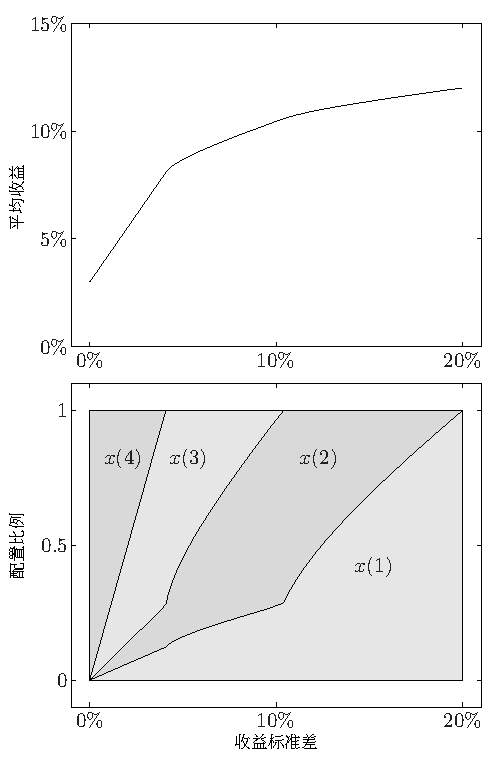
\includegraphics[width=.65\textwidth]{figures/ch04-12.pdf}
\caption*{图4.12\quad 上图：简单投资组合优化的最优风险收益权衡曲线。左端点对应全部投资于无风险资产，因而标准差为零。右端点对应全部投资于平均收益最高的资产1。下图：对应的最优配置。}
\end{figure}

% Source PDF page 202 (printed p. 188)
\section*{文献说明}
\addcontentsline{toc}{section}{文献说明}
线性规划自20世纪40年代以来得到广泛研究，是许多优秀著作的主题，包括Dantzig [Dan63]、Luenberger [Lue84]、Schrijver [Sch86]、Papadimitriou和Steiglitz [PS98]、Bertsimas和Tsitsiklis [BT97]、Vanderbei [Van96]，以及Roos、Terlaky和Vial [RTV97]。Dantzig和Schrijver还详细介绍了线性规划史。较新的综述见Todd [Tod02]。

Schaible [Sch82, Sch83] 概述了分式规划，包括线性分式问题及凸凹分式问题等推广，见习题4.7。例4.7的经济增长模型出自von Neumann [vN46]。

二次规划研究始于20世纪50年代，例如Frank和Wolfe [FW56]、Markowitz [Mar56]、Hildreth [Hil57]；部分动机来自第155页的投资组合优化问题（Markowitz [Mar52]），以及第154页的随机成本LP，见Freund [Fre56]。

二阶锥规划较晚才引起关注，始于Nesterov和Nemirovski [NN94, §6.2.3]。关于SOCP理论和应用的综述，见Alizadeh和Goldfarb [AG03]、Ben-Tal和Nemirovski [BTN01, lecture 3]（其中称为锥二次规划），以及Lobo、Vandenberghe、Boyd和Lebret [LVBL98]。

鲁棒线性规划以及更一般的鲁棒凸优化，始于Ben-Tal和Nemirovski [BTN98, BTN99] 与El Ghaoui和Lebret [EL97]。Goldfarb和Iyengar [GI03a, GI03b] 讨论鲁棒QCQP及其在投资组合优化中的应用。El Ghaoui、Oustry和Lebret [EOL98] 专门研究鲁棒半正定规划。

几何规划自20世纪60年代起为人所知。Duffin、Peterson和Zener [DPZ67] 与Zener [Zen71] 最先倡导将其用于工程设计。Peterson [Pet76] 与Ecker [Eck80] 介绍了20世纪70年代的进展。这些文章和书籍还包括工程应用例子，特别是化学工程和土木工程。Fishburn和Dunlop [FD85]、Sapatnekar、Rao、Vaidya和Kang [SRVK93]，以及Hershenson、Boyd和Lee [HBL01] 将几何规划用于集成电路设计。第163页的悬臂梁设计例子取自Vanderplaats [Van84, page 147]。第165页Perron--Frobenius特征值的变分刻画证明见Berman和Plemmons [BP94, page 31]。

Nesterov和Nemirovski [NN94, chapter 4] 将锥形式问题（4.49）作为非线性凸优化的一种标准问题格式引入。Ben-Tal和Nemirovski [BTN01] 进一步发展了锥规划方法，并介绍大量应用。

Alizadeh [Ali91] 与Nesterov和Nemirovski [NN94, §6.4] 最先系统研究半正定规划，并指出其在凸优化中的广泛应用。20世纪90年代，半正定规划的后续研究由组合优化、控制、通信与信号处理及其他工程领域的应用推动。组合优化见Goemans和Williamson [GW95]；控制见Boyd、El Ghaoui、Feron和Balakrishnan [BEFB94]、Scherer、Gahinet和Chilali [SGC97]、Dullerud和Paganini [DP00]；通信与信号处理见Luo [Luo03]、Davidson、Luo、Wong和Ma [DLW00, MDW$^+$02]。Wolkowicz、Saigal和Vandenberghe编辑的书 [WSV00]，以及Todd [Tod01]、Lewis和Overton [LO96]、Vandenberghe和Boyd [VB95] 的文章，提供了综述和广泛的参考文献。第170页给出简单例子的SDP与矩问题之间的联系，由Bertsimas和Sethuraman [BS00]、Nesterov [Nes00] 和Lasserre [Las02] 详细研究。最快混合马尔可夫链问题出自Boyd、Diaconis和Xiao [BDX04]。

多准则优化和Pareto最优性是经济学的基本工具，见Pareto [Par71]、Debreu [Deb59]、Luenberger [Lue95]。例4.9的结果称为Gauss--Markov定理，见Kailath、Sayed和Hassibi [KSH00, page 97]。

\section*{习题}
\addcontentsline{toc}{section}{习题}
% Source PDF page 203 (printed p. 189)
\subsection*{基本术语与最优性条件}
\paragraph{4.1}考虑优化问题
\[
\begin{array}{ll}\text{最小化}&f_0(x_1,x_2)\\\text{约束为}&2x_1+x_2\ge1,\\&x_1+3x_2\ge1,\\&x_1\ge0,\quad x_2\ge0.\end{array}
\]
画出可行集示意图。对下列每个目标函数，给出最优集和最优值。
\begin{enumerate}[label=(\alph*)]
\item $f_0(x_1,x_2)=x_1+x_2$。
\item $f_0(x_1,x_2)=-x_1-x_2$。
\item $f_0(x_1,x_2)=x_1$。
\item $f_0(x_1,x_2)=\max\{x_1,x_2\}$。
\item $f_0(x_1,x_2)=x_1^2+9x_2^2$。
\end{enumerate}

\paragraph{4.2}考虑优化问题
\[
\text{最小化}\quad f_0(x)=-\sum_{i=1}^m\log(b_i-a_i^\T x),
\]
定义域为 $\dom f_0=\{x\mid Ax\prec b\}$，其中 $A\in\R^{m\times n}$，各行为 $a_i^\T$。假设 $\dom f_0$ 非空。

证明下列事实，其中包括第141页未经证明引用的结果。
\begin{enumerate}[label=(\alph*)]
\item $\dom f_0$ 无界，当且仅当存在 $v\ne0$ 使 $Av\preceq0$。
\item $f_0$ 无下界，当且仅当存在 $v$ 使 $Av\preceq0$、$Av\ne0$。提示：存在满足 $Av\preceq0$、$Av\ne0$ 的 $v$，当且仅当不存在 $z\succ0$ 使 $A^\T z=0$。这由第50页例2.21的择一定理推出。
\item 若 $f_0$ 有下界，则其最小值可以达到，即存在满足最优性条件（4.23）的 $x$。
\item 最优集是仿射集：$X_{\mathrm{opt}}=\{x^\star+v\mid Av=0\}$，其中 $x^\star$ 是任意最优点。
\end{enumerate}

\paragraph{4.3}证明 $x^\star=(1,1/2,-1)$ 对优化问题
\[
\begin{array}{ll}\text{最小化}&(1/2)x^\T Px+q^\T x+r\\\text{约束为}&-1\le x_i\le1,\quad i=1,2,3\end{array}
\]
最优，其中
\[
P=\begin{bmatrix}13&12&-2\\12&17&6\\-2&6&12\end{bmatrix},\qquad
q=\begin{bmatrix}-22.0\\-14.5\\13.0\end{bmatrix},\qquad r=1.
\]

\paragraph{4.4}[P. Parrilo] \textbf{对称性与凸优化。}设 $G=\{Q_1,\ldots,Q_k\}\subseteq\R^{n\times n}$ 为群，即对乘法和求逆封闭。若对所有 $x$、所有 $i=1,\ldots,k$，有 $f(Q_ix)=f(x)$，就称函数 $f:\R^n\to\R$ 是 $G$-不变的，或关于 $G$ 对称。定义 $\bar x=(1/k)\sum_{i=1}^k Q_ix$，即 $x$ 在其 $G$-轨道上的平均。定义 $G$ 的不动子空间为
\[
\mathcal F=\{x\mid Q_ix=x,\ i=1,\ldots,k\}.
\]
\begin{enumerate}[label=(\alph*)]
\item 证明对任意 $x\in\R^n$，有 $\bar x\in\mathcal F$。
% Source PDF page 204 (printed p. 190)
\item 证明，若 $f:\R^n\to\R$ 凸且 $G$-不变，则 $f(\bar x)\le f(x)$。
\item 若优化问题
\[
\begin{array}{ll}\text{最小化}&f_0(x)\\\text{约束为}&f_i(x)\le0,\quad i=1,\ldots,m\end{array}
\]
的目标 $f_0$ 为 $G$-不变函数，可行集也是 $G$-不变的，即对 $i=1,\ldots,k$，
\[
f_1(x)\le0,\ldots,f_m(x)\le0\ \Longrightarrow\ f_1(Q_ix)\le0,\ldots,f_m(Q_ix)\le0,
\]
就称问题 $G$-不变。证明：若问题凸且 $G$-不变，并存在最优点，则 $\mathcal F$ 中存在最优点。换言之，不失一般性，可以向问题加入等式约束 $x\in\mathcal F$。
\item 例如，设 $f$ 凸且对称，即对每个置换 $P$ 有 $f(Px)=f(x)$。证明：若 $f$ 有最小点，就有形如 $\alpha\one$ 的最小点。这意味着在 $x\in\R^n$ 上最小化 $f$，也可以改为在 $t\in\R$ 上最小化 $f(t\one)$。
\end{enumerate}

\paragraph{4.5}\textbf{等价凸问题。}证明以下三个凸问题等价，仔细说明如何由每一个问题的解得到其他问题的解。数据为矩阵 $A\in\R^{m\times n}$（各行为 $a_i^\T$）、向量 $b\in\R^m$ 和常数 $M>0$。
\begin{enumerate}[label=(\alph*)]
\item 鲁棒最小二乘问题
\[
\text{最小化}\quad\sum_{i=1}^m\phi(a_i^\T x-b_i),
\]
变量为 $x\in\R^n$，其中 $\phi:\R\to\R$ 定义为
\[
\phi(u)=\begin{cases}u^2,&|u|\le M,\\M(2|u|-M),&|u|>M.\end{cases}
\]
这个函数称为Huber罚函数，见§6.1.2。
\item 可变权重最小二乘问题
\[
\begin{array}{ll}\text{最小化}&\displaystyle\sum_{i=1}^m\frac{(a_i^\T x-b_i)^2}{w_i+1}+M^2\one^\T w\\\text{约束为}&w\succeq0,\end{array}
\]
变量为 $x\in\R^n,w\in\R^m$，定义域 $\mathcal D=\{(x,w)\in\R^n\times\R^m\mid w\succ-\one\}$。提示：固定 $x$，对 $w$ 优化，建立与(a)的关系。

此问题可解释为允许调整第 $i$ 个残差权重的加权最小二乘。$w_i=0$ 时权重为一，增大 $w_i$ 则权重下降。目标第二项惩罚较大的 $w$，即惩罚较大的权重调整。
\item 二次规划
\[
\begin{array}{ll}\text{最小化}&\displaystyle\sum_{i=1}^m(u_i^2+2Mv_i)\\\text{约束为}&-u-v\preceq Ax-b\preceq u+v,\\&0\preceq u\preceq M\one,\\&v\succeq0.\end{array}
\]
\end{enumerate}

% Source PDF page 205 (printed p. 191)
\paragraph{4.6}\textbf{处理凸等式约束。}凸优化问题只能有线性等式约束函数。不过，在一些特殊情况下，可以处理凸等式约束函数，即 $h(x)=0$ 形式的约束，其中 $h$ 凸。本题研究这个思路。

考虑优化问题
\begin{equation}
\begin{array}{ll}\text{最小化}&f_0(x)\\\text{约束为}&f_i(x)\le0,\quad i=1,\ldots,m,\\&h(x)=0,\end{array}\tag{4.65}
\end{equation}
其中 $f_i,h$ 均为定义域为 $\R^n$ 的凸函数。除非 $h$ 仿射，否则这不是凸优化问题。考虑将凸等式放松为凸不等式的相关问题
\begin{equation}
\begin{array}{ll}\text{最小化}&f_0(x)\\\text{约束为}&f_i(x)\le0,\quad i=1,\ldots,m,\\&h(x)\le0.\end{array}\tag{4.66}
\end{equation}
它当然是凸问题。

现在假设能保证，凸问题（4.66）的任意最优解 $x^\star$ 均满足 $h(x^\star)=0$，即不等式 $h(x)\le0$ 在解处总活跃。于是可通过求解凸问题（4.66）解出非凸问题（4.65）。证明若存在指标 $r$ 满足下列条件，就属于这种情况：
\begin{itemize}
\item $f_0$ 关于 $x_r$ 单调递增；
\item $f_1,\ldots,f_m$ 关于 $x_r$ 非减；
\item $h$ 关于 $x_r$ 单调递减。
\end{itemize}
习题4.31和4.58将给出具体例子。

\paragraph{4.7}\textbf{凸凹分式问题。}考虑问题
\[
\begin{array}{ll}\text{最小化}&f_0(x)/(c^\T x+d)\\\text{约束为}&f_i(x)\le0,\quad i=1,\ldots,m,\\&Ax=b,\end{array}
\]
其中 $f_0,f_1,\ldots,f_m$ 凸，目标定义域为 $\{x\in\dom f_0\mid c^\T x+d>0\}$。
\begin{enumerate}[label=(\alph*)]
\item 证明这是拟凸优化问题。
\item 证明它等价于
\[
\begin{array}{ll}\text{最小化}&g_0(y,t)\\\text{约束为}&g_i(y,t)\le0,\quad i=1,\ldots,m,\\&Ay=bt,\\&c^\T y+dt=1,\end{array}
\]
其中 $g_i$ 为 $f_i$ 的透视函数，见§3.2.6。变量为 $y\in\R^n,t\in\R$。证明此问题凸。
\item 沿用类似论证，为凸凹分式问题
\[
\begin{array}{ll}\text{最小化}&f_0(x)/h(x)\\\text{约束为}&f_i(x)\le0,\quad i=1,\ldots,m,\\&Ax=b\end{array}
\]
推导凸表述，
% Source PDF page 206 (printed p. 192)
其中 $f_0,f_1,\ldots,f_m$ 凸，$h$ 凹，目标定义域为 $\{x\in\dom f_0\cap\dom h\mid h(x)>0\}$，且处处有 $f_0(x)\ge0$。

例如，将你的技巧用于无约束问题，其中
\[
f_0(x)=\tr F(x)/m,\qquad h(x)=(\det(F(x)))^{1/m},
\]
$\dom(f_0/h)=\{x\mid F(x)\succ0\}$，$F(x)=F_0+x_1F_1+\cdots+x_nF_n$，矩阵 $F_i\in\mathbf S^m$ 给定。此问题最小化仿射矩阵函数 $F(x)$ 的特征值算术平均与几何平均之比。
\end{enumerate}

\subsection*{线性优化问题}
\paragraph{4.8}\textbf{若干简单LP。}给出下列各LP的显式解。
\begin{enumerate}[label=(\alph*)]
\item 在仿射集上最小化线性函数。
\[
\begin{array}{ll}\text{最小化}&c^\T x\\\text{约束为}&Ax=b.\end{array}
\]
\item 在半空间上最小化线性函数。
\[
\begin{array}{ll}\text{最小化}&c^\T x\\\text{约束为}&a^\T x\le b,\end{array}
\]
其中 $a\ne0$。
\item 在长方体上最小化线性函数。
\[
\begin{array}{ll}\text{最小化}&c^\T x\\\text{约束为}&l\preceq x\preceq u,\end{array}
\]
其中 $l\preceq u$。
\item 在概率单纯形上最小化线性函数。
\[
\begin{array}{ll}\text{最小化}&c^\T x\\\text{约束为}&\one^\T x=1,\quad x\succeq0.\end{array}
\]
若将等式约束替换为不等式 $\one^\T x\le1$，会怎样？

此LP可解释为简单投资组合优化。向量 $x$ 表示总预算在各资产上的配置，$x_i$ 为投资于资产 $i$ 的比例。各项投资回报固定，为 $-c_i$，所以希望最大化的总回报为 $-c^\T x$。若将预算等式改为 $\one^\T x\le1$，就可以选择不投资一部分预算。
\item 在有总预算约束的单位盒上最小化线性函数。
\[
\begin{array}{ll}\text{最小化}&c^\T x\\\text{约束为}&\one^\T x=\alpha,\quad0\preceq x\preceq\one,\end{array}
\]
其中 $\alpha$ 为0到 $n$ 之间的整数。若 $\alpha$ 非整数，但满足 $0\le\alpha\le n$，会怎样？若将等式改为 $\one^\T x\le\alpha$ 呢？
\item 在有加权预算约束的单位盒上最小化线性函数。
\[
\begin{array}{ll}\text{最小化}&c^\T x\\\text{约束为}&d^\T x=\alpha,\quad0\preceq x\preceq\one,\end{array}
\]
其中 $d\succ0$、$0\le\alpha\le\one^\T d$。
\end{enumerate}

% Source PDF page 207 (printed p. 193)
\paragraph{4.9}\textbf{方阵LP。}考虑LP
\[
\begin{array}{ll}\text{最小化}&c^\T x\\\text{约束为}&Ax\preceq b,\end{array}
\]
其中 $A$ 为非奇异方阵。证明最优值为
\[
p^\star=\begin{cases}c^\T A^{-1}b,&A^{-\T}c\preceq0,\\-\infty,&\text{其他情形。}\end{cases}
\]

\paragraph{4.10}\textbf{将一般LP化为标准形式。}补全§4.3第147页的细节。详细说明标准形式LP与原LP的可行集、最优解及最优值之间的关系。

\paragraph{4.11}\textbf{涉及 $\ell_1$ 和 $\ell_\infty$ 范数的问题。}将下列问题表述为LP，详细说明每个问题的最优解与其等价LP的解之间的关系。
\begin{enumerate}[label=(\alph*)]
\item 最小化 $\norm{Ax-b}_\infty$，即 $\ell_\infty$ 范数逼近。
\item 最小化 $\norm{Ax-b}_1$，即 $\ell_1$ 范数逼近。
\item 在 $\norm{x}_\infty\le1$ 下最小化 $\norm{Ax-b}_1$。
\item 在 $\norm{Ax-b}_\infty\le1$ 下最小化 $\norm{x}_1$。
\item 最小化 $\norm{Ax-b}_1+\norm{x}_\infty$。
\end{enumerate}
各题中 $A\in\R^{m\times n},b\in\R^m$ 给定。更多逼近和约束逼近问题见§6.1。

\paragraph{4.12}\textbf{网络流问题。}考虑一个有 $n$ 个结点、每对结点间均有有向连接的网络。变量为每条连接上的流量：$x_{ij}$ 表示从结点 $i$ 到结点 $j$ 的流量。连接 $i$ 到 $j$ 上流的成本为 $c_{ij}x_{ij}$，其中 $c_{ij}$ 为给定常数。全网络总成本为
\[
C=\sum_{i,j=1}^n c_{ij}x_{ij}.
\]
每条连接的流量 $x_{ij}$ 还有给定下界 $l_{ij}$（通常假设非负）和上界 $u_{ij}$。

结点 $i$ 的外部供给为 $b_i$，其中 $b_i>0$ 表示外部流从结点 $i$ 进入网络，$b_i<0$ 表示数量为 $|b_i|$ 的流从结点 $i$ 流出网络。假设 $\one^\T b=0$，即外部总供给等于外部总需求。每个结点都满足流量守恒：沿连接进入结点 $i$ 的总流量加外部供给，再减去沿连接流出的总流量，等于零。

问题是在上述约束下最小化网络总流成本。将其表述为LP。

\paragraph{4.13}\textbf{系数为区间的鲁棒LP。}考虑变量为 $x\in\R^n$ 的问题
\[
\begin{array}{ll}\text{最小化}&c^\T x\\\text{约束为}&Ax\preceq b\quad\text{对所有 }A\in\mathcal A,\end{array}
\]
其中 $\mathcal A\subseteq\R^{m\times n}$ 为
\[
\mathcal A=\{A\in\R^{m\times n}\mid\bar A_{ij}-V_{ij}\le A_{ij}\le\bar A_{ij}+V_{ij},\ i=1,\ldots,m,\ j=1,\ldots,n\}.
\]
矩阵 $\bar A,V$ 给定。此问题可解释为LP，其矩阵 $A$ 的每个系数只知道位于一个区间内，要求 $x$ 对全部可能系数取值均满足约束。

将其表示为LP。构造的LP应当高效，即维数不应随 $n$ 或 $m$ 指数增长。

% Source PDF page 208 (printed p. 194)
\paragraph{4.14}\textbf{无穷范数下的矩阵逼近。}矩阵 $A\in\R^{m\times n}$ 的 $\ell_\infty$ 诱导范数，记为 $\norm{A}_\infty$，为
\[
\norm{A}_\infty=\sup_{x\ne0}\frac{\norm{Ax}_\infty}{\norm{x}_\infty}
=\max_{i=1,\ldots,m}\sum_{j=1}^n|a_{ij}|.
\]
这个范数也称为最大行和范数，原因显而易见，见§A.1.5。考虑以其他矩阵的线性组合，在最大行和范数下逼近一个矩阵的问题。具体而言，给定 $k+1$ 个矩阵 $A_0,\ldots,A_k\in\R^{m\times n}$，需找 $x\in\R^k$，使
\[
\norm{A_0+x_1A_1+\cdots+x_kA_k}_\infty
\]
最小。将其表示为LP，解释所引入额外变量的意义。仔细说明LP表述如何求解原问题，例如，LP可行集与原问题是什么关系？

\paragraph{4.15}\textbf{布尔LP的放松。}布尔线性规划中，变量 $x$ 的各分量被限制为零或一：
\begin{equation}
\begin{array}{ll}\text{最小化}&c^\T x\\\text{约束为}&Ax\preceq b,\\&x_i\in\{0,1\},\quad i=1,\ldots,n.\end{array}\tag{4.67}
\end{equation}
一般而言，即使可行集有限、至多包含 $2^n$ 个点，这类问题也很难求解。

一种称为放松的一般方法，是将 $x_i$ 为零或一的约束替换为线性不等式 $0\le x_i\le1$：
\begin{equation}
\begin{array}{ll}\text{最小化}&c^\T x\\\text{约束为}&Ax\preceq b,\\&0\le x_i\le1,\quad i=1,\ldots,n.\end{array}\tag{4.68}
\end{equation}
称其为布尔LP（4.67）的LP放松。LP放松远比原布尔LP容易求解。
\begin{enumerate}[label=(\alph*)]
\item 证明LP放松（4.68）的最优值是布尔LP（4.67）最优值的下界。若LP放松不可行，对布尔LP能作何判断？
\item 有时LP放松的某个解满足 $x_i\in\{0,1\}$，此时能作何判断？
\end{enumerate}

\paragraph{4.16}\textbf{最小燃料最优控制。}考虑线性动态系统，状态为 $x(t)\in\R^n$（$t=0,\ldots,N$），执行器或输入信号为 $u(t)\in\R$（$t=0,\ldots,N-1$）。系统动态为线性递推
\[
x(t+1)=Ax(t)+bu(t),\quad t=0,\ldots,N-1,
\]
其中 $A\in\R^{n\times n},b\in\R^n$ 给定。假设初始状态为零，即 $x(0)=0$。

最小燃料最优控制问题是选择输入 $u(0),\ldots,u(N-1)$，使总耗油量
\[
F=\sum_{t=0}^{N-1}f(u(t))
\]
最小，
% Source PDF page 209 (printed p. 195)
并满足 $x(N)=x^{\mathrm{des}}$。其中 $N$ 为给定时间范围，$x^{\mathrm{des}}\in\R^n$ 为给定的期望最终状态或目标状态。函数 $f:\R\to\R$ 是执行器的耗油映射，给出耗油量随执行器信号幅度的变化。本题采用
\[
f(a)=\begin{cases}|a|,&|a|\le1,\\2|a|-1,&|a|>1.\end{cases}
\]
这意味着信号在 $-1$ 到 $1$ 之间时，耗油量与信号绝对值成正比；信号更大时，边际燃料效率减半。将最小燃料最优控制问题表述为LP。

\paragraph{4.17}\textbf{最优活动水平。}考虑选择 $n$ 个非负活动水平 $x_1,\ldots,x_n$。活动消耗有限的 $m$ 种资源。活动 $j$ 消耗资源 $i$ 的数量为 $A_{ij}x_j$，$A_{ij}$ 给定。资源消耗可加，所以资源 $i$ 的总消耗为 $c_i=\sum_{j=1}^n A_{ij}x_j$。（通常 $A_{ij}\ge0$，即活动 $j$ 消耗资源 $i$；但允许 $A_{ij}<0$，这表示活动 $j$ 实际上以副产品的形式产生资源 $i$。）每种资源消耗有限，要求 $c_i\le c_i^{\max}$，其中 $c_i^{\max}$ 给定。每项活动产生收益，它是活动水平的分段线性凹函数：
\[
r_j(x_j)=\begin{cases}p_jx_j,&0\le x_j\le q_j,\\p_jq_j+p_j^{\mathrm{disc}}(x_j-q_j),&x_j\ge q_j.\end{cases}
\]
其中 $p_j>0$ 为基本价格，$q_j>0$ 为数量折扣阈值，$p_j^{\mathrm{disc}}$ 为活动 $j$ 的产品的数量折扣价格，满足 $0<p_j^{\mathrm{disc}}<p_j$。总收益为各项活动收益之和 $\sum_{j=1}^n r_j(x_j)$。

目标是在满足资源限制时选择使总收益最大的活动水平。说明如何将此问题表述为LP。

\paragraph{4.18}\textbf{分离超平面与球面。}给定 $\R^n$ 中两组点 $\{v_1,v_2,\ldots,v_K\}$ 和 $\{w_1,w_2,\ldots,w_L\}$。将下列两个问题表述为LP可行性问题。
\begin{enumerate}[label=(\alph*)]
\item 确定分离两组点的超平面，即求 $a\in\R^n,b\in\R$，$a\ne0$，使
\[
a^\T v_i\le b,\quad i=1,\ldots,K,\qquad a^\T w_i\ge b,\quad i=1,\ldots,L.
\]
注意要求 $a\ne0$，所以表述中须排除平凡解 $a=0,b=0$。可以假设
\[
\rank\begin{bmatrix}v_1&v_2&\cdots&v_K&w_1&w_2&\cdots&w_L\\1&1&\cdots&1&1&1&\cdots&1\end{bmatrix}=n+1,
\]
即这 $K+L$ 个点的仿射包维数为 $n$。
\item 确定分离两组点的球面，即求 $x_c\in\R^n,R\ge0$，使
\[
\norm{v_i-x_c}_2\le R,\quad i=1,\ldots,K,\qquad
\norm{w_i-x_c}_2\ge R,\quad i=1,\ldots,L.
\]
这里 $x_c$ 为球心，$R$ 为半径。
\end{enumerate}
关于分离超平面、分离球面及相关主题的更多内容，见第8章。

% Source PDF page 210 (printed p. 196)
\paragraph{4.19}考虑问题
\[
\begin{array}{ll}\text{最小化}&\norm{Ax-b}_1/(c^\T x+d)\\\text{约束为}&\norm{x}_\infty\le1,\end{array}
\]
其中 $A\in\R^{m\times n},b\in\R^m,c\in\R^n,d\in\R$。假设 $d>\norm{c}_1$，从而对所有可行 $x$ 都有 $c^\T x+d>0$。
\begin{enumerate}[label=(\alph*)]
\item 证明这是拟凸优化问题。
\item 证明它等价于以下凸优化问题，变量为 $y\in\R^n,t\in\R$：
\[
\begin{array}{ll}\text{最小化}&\norm{Ay-bt}_1\\\text{约束为}&\norm{y}_\infty\le t,\\&c^\T y+dt=1.\end{array}
\]
\end{enumerate}

\paragraph{4.20}\textbf{无线通信系统中的功率分配。}考虑 $n$ 个发射机，以功率 $p_1,\ldots,p_n\ge0$ 向 $n$ 个接收机发送信号。这些功率是优化变量。用 $G\in\R^{n\times n}$ 表示发射机至接收机的路径增益矩阵；$G_{ij}\ge0$ 为发射机 $j$ 到接收机 $i$ 的路径增益。接收机 $i$ 的信号功率为 $S_i=G_{ii}p_i$，干扰功率为 $I_i=\sum_{k\ne i}G_{ik}p_k$。接收机 $i$ 的信干噪比（SINR）为 $S_i/(I_i+\sigma_i)$，其中 $\sigma_i>0$ 为接收机 $i$ 的自身噪声功率。目标是最大化所有接收机中的最小SINR，即最大化
\[
\min_{i=1,\ldots,n}\frac{S_i}{I_i+\sigma_i}.
\]
除显然的 $p_i\ge0$ 外，功率还需满足若干约束。首先每个发射机有最大允许功率，即 $p_i\le P_i^{\max}$，其中 $P_i^{\max}>0$ 给定。此外，发射机分为若干组，每组共享电源，所以每组发射功率有总量约束。具体地，给定 $\{1,\ldots,n\}$ 的子集 $K_1,\ldots,K_m$，满足 $K_1\cup\cdots\cup K_m=\{1,\ldots,n\}$，且 $j\ne l$ 时 $K_j\cap K_l=\varnothing$。对每组 $K_l$，相关发射机总功率不能超过 $P_l^{\mathrm{gp}}>0$：
\[
\sum_{k\in K_l}p_k\le P_l^{\mathrm{gp}},\quad l=1,\ldots,m.
\]
最后，每个接收机的总接收功率有上限 $P_k^{\mathrm{rc}}>0$：
\[
\sum_{k=1}^nG_{ik}p_k\le P_i^{\mathrm{rc}},\quad i=1,\ldots,n.
\]
这反映了总接收功率过大时接收机会饱和。将SINR最大化问题表述为广义线性分式规划。

\subsection*{二次优化问题}
\paragraph{4.21}\textbf{若干简单QCQP。}给出下列各QCQP的显式解。
\begin{enumerate}[label=(\alph*)]
\item 在以原点为中心的椭球上最小化线性函数。
\[
\begin{array}{ll}\text{最小化}&c^\T x\\\text{约束为}&x^\T Ax\le1,\end{array}
\]
其中 $A\in\mathbf S_{++}^n,c\ne0$。若问题非凸，即 $A\notin\mathbf S_+^n$，解是什么？

% Source PDF page 211 (printed p. 197)
\item 在椭球上最小化线性函数。
\[
\begin{array}{ll}\text{最小化}&c^\T x\\\text{约束为}&(x-x_c)^\T A(x-x_c)\le1,\end{array}
\]
其中 $A\in\mathbf S_{++}^n,c\ne0$。
\item 在以原点为中心的椭球上最小化二次型。
\[
\begin{array}{ll}\text{最小化}&x^\T Bx\\\text{约束为}&x^\T Ax\le1,\end{array}
\]
其中 $A\in\mathbf S_{++}^n,B\in\mathbf S_+^n$。也考虑 $B\notin\mathbf S_+^n$ 的非凸推广，见§B.1。
\end{enumerate}

\paragraph{4.22}考虑QCQP
\[
\begin{array}{ll}\text{最小化}&(1/2)x^\T Px+q^\T x+r\\\text{约束为}&x^\T x\le1,\end{array}
\]
其中 $P\in\mathbf S_{++}^n$。证明 $x^\star=-(P+\lambda I)^{-1}q$，其中 $\lambda=\max\{0,\bar\lambda\}$，$\bar\lambda$ 是非线性方程
\[
q^\T(P+\lambda I)^{-2}q=1
\]
的最大解。

\paragraph{4.23}\textbf{用QCQP求 $\ell_4$ 范数逼近。}将 $\ell_4$ 范数逼近问题
\[
\text{最小化}\quad\norm{Ax-b}_4=\left(\sum_{i=1}^m(a_i^\T x-b_i)^4\right)^{1/4}
\]
表述为QCQP。矩阵 $A\in\R^{m\times n}$（各行为 $a_i^\T$）和向量 $b\in\R^m$ 给定。

\paragraph{4.24}\textbf{复数 $\ell_1,\ell_2,\ell_\infty$ 范数逼近。}考虑问题
\[
\text{最小化}\quad\norm{Ax-b}_p,
\]
其中 $A\in\C^{m\times n},b\in\C^m$，变量为 $x\in\C^n$。复数 $\ell_p$ 范数定义为
\[
\norm{y}_p=\left(\sum_{i=1}^m|y_i|^p\right)^{1/p},\quad p\ge1,
\]
并定义 $\norm{y}_\infty=\max_{i=1,\ldots,m}|y_i|$。对 $p=1,2,\infty$，将复数 $\ell_p$ 范数逼近问题表示为具有实变量和实数据的QCQP或SOCP。

\paragraph{4.25}\textbf{两组椭球的线性分离。}给定 $K+L$ 个椭球
\[
\mathcal E_i=\{P_iu+q_i\mid\norm{u}_2\le1\},\quad i=1,\ldots,K+L,
\]
其中 $P_i\in\mathbf S^n$。我们希望寻找超平面，将 $\mathcal E_1,\ldots,\mathcal E_K$ 与 $\mathcal E_{K+1},\ldots,\mathcal E_{K+L}$ 严格分离，即求 $a\in\R^n,b\in\R$，使
\[
\begin{aligned}
a^\T x+b&>0,&&x\in\mathcal E_1\cup\cdots\cup\mathcal E_K,\\
a^\T x+b&<0,&&x\in\mathcal E_{K+1}\cup\cdots\cup\mathcal E_{K+L},
\end{aligned}
\]
或证明这样的超平面不存在。将其表示为SOCP可行性问题。

\paragraph{4.26}\textbf{将双曲约束写为SOC约束。}验证 $x\in\R^n,y,z\in\R$ 满足
\[
x^\T x\le yz,\qquad y\ge0,\quad z\ge0
\]
当且仅当
\[
\left\|\begin{bmatrix}2x\\y-z\end{bmatrix}\right\|_2\le y+z,\qquad y\ge0,\quad z\ge0.
\]
利用这一事实，将以下问题写成SOCP。

% Source PDF page 212 (printed p. 198)
\begin{enumerate}[label=(\alph*)]
\item 最大化调和平均。
\[
\text{最大化}\quad\left(\sum_{i=1}^m\frac1{a_i^\T x-b_i}\right)^{-1},
\]
定义域为 $\{x\mid Ax\succ b\}$，其中 $a_i^\T$ 是 $A$ 的第 $i$ 行。
\item 最大化几何平均。
\[
\text{最大化}\quad\left(\prod_{i=1}^m(a_i^\T x-b_i)\right)^{1/m},
\]
定义域为 $\{x\mid Ax\succeq b\}$，其中 $a_i^\T$ 是 $A$ 的第 $i$ 行。
\end{enumerate}

\paragraph{4.27}\textbf{通过SOCP最小化矩阵分式。}将以下问题表示为SOCP：
\[
\begin{array}{ll}\text{最小化}&(Ax+b)^\T(I+B\diag(x)B^\T)^{-1}(Ax+b)\\\text{约束为}&x\succeq0,\end{array}
\]
其中 $A\in\R^{m\times n},b\in\R^m,B\in\R^{m\times n}$，变量为 $x\in\R^n$。

提示：先证明问题等价于
\[
\begin{array}{ll}\text{最小化}&v^\T v+w^\T\diag(x)^{-1}w\\\text{约束为}&v+Bw=Ax+b,\\&x\succeq0,\end{array}
\]
变量为 $v\in\R^m,w,x\in\R^n$。（若 $x_i=0$，则 $w_i=0$ 时将 $w_i^2/x_i$ 解释为零，否则解释为 $\infty$。）然后使用习题4.26的结果。

\paragraph{4.28}\textbf{鲁棒二次规划。}§4.4.2将鲁棒线性规划作为二阶锥规划的应用。本题考虑凸二次规划
\[
\begin{array}{ll}\text{最小化}&(1/2)x^\T Px+q^\T x+r\\\text{约束为}&Ax\preceq b\end{array}
\]
的类似鲁棒变体。为简单起见，假设只有矩阵 $P$ 有误差，其余参数 $q,r,A,b$ 精确已知。鲁棒二次规划定义为
\[
\begin{array}{ll}\text{最小化}&\sup_{P\in\mathcal E}((1/2)x^\T Px+q^\T x+r)\\\text{约束为}&Ax\preceq b,\end{array}
\]
其中 $\mathcal E$ 是所有可能矩阵 $P$ 的集合。

对以下各个 $\mathcal E$，将鲁棒QP表示为凸问题，尽量具体。如果能写成标准形式，例如QP、QCQP、SOCP、SDP，请指出。
\begin{enumerate}[label=(\alph*)]
\item 有限矩阵集：$\mathcal E=\{P_1,\ldots,P_K\}$，其中 $P_i\in\mathbf S_+^n$（$i=1,\ldots,K$）。
\item 由标称值 $P_0\in\mathbf S_+^n$ 及偏差 $P-P_0$ 的特征值界给出的集合：
\[
\mathcal E=\{P\in\mathbf S^n\mid-\gamma I\preceq P-P_0\preceq\gamma I\},
\]
其中 $\gamma\in\R,P_0\in\mathbf S_+^n$。
\item 矩阵椭球：
\[
\mathcal E=\left\{P_0+\sum_{i=1}^K P_iu_i\ \middle|\ \norm{u}_2\le1\right\}.
\]
可假设 $P_i\in\mathbf S_+^n$（$i=0,\ldots,K$）。
\end{enumerate}

% Source PDF page 213 (printed p. 199)
\paragraph{4.29}\textbf{最大化满足线性不等式的概率。}设 $c$ 是 $\R^n$ 中的正态随机变量，均值为 $\bar c$，协方差矩阵为 $R$。考虑问题
\[
\begin{array}{ll}\text{最大化}&\Prob(c^\T x\ge\alpha)\\\text{约束为}&Fx\preceq g,\quad Ax=b.\end{array}
\]
假设存在可行点 $\widetilde x$ 使 $\bar c^\T\widetilde x\ge\alpha$，证明此问题等价于凸或拟凸优化问题。若凸，将其表述为QP、QCQP或SOCP；若拟凸，说明如何通过求解一系列QP、QCQP或SOCP可行性问题求解。

\subsection*{几何规划}
\paragraph{4.30}温度为 $T$ 的热流体流过一根长度固定、圆形截面半径为 $r$ 的管道，$T$ 为高于环境温度的度数。管道外包裹厚度 $w\ll r$ 的绝热层，以减少经管壁散热。设计变量为 $T,r,w$。

热损失近似正比于 $Tr/w$，所以固定寿命期内散热引起的能源成本为 $\alpha_1Tr/w$。管壁厚度固定，管道成本近似正比于材料总量，即 $\alpha_2r$。绝热层成本也近似正比于绝热材料总量，即 $\alpha_3rw$，这里利用 $w\ll r$。总成本为这三项之和。

沿管道的热流完全来自流体流动，流速固定，故热流为 $\alpha_4Tr^2$。常数 $\alpha_i$ 均为正，变量 $T,r,w$ 也为正。

问题是在总成本上界 $C_{\max}$ 及约束
\[
T_{\min}\le T\le T_{\max},\quad r_{\min}\le r\le r_{\max},\quad
w_{\min}\le w\le w_{\max},\quad w\le0.1r
\]
下，最大化沿管道的总热流。将此问题表示为几何规划。

\paragraph{4.31}\textbf{最优梁设计的递推表述。}证明GP（4.46）等价于GP
\[
\begin{array}{ll}
\text{最小化}&\displaystyle\sum_{i=1}^N w_ih_i\\
\text{约束为}&w_i/w_{\max}\le1,\quad w_{\min}/w_i\le1,\quad i=1,\ldots,N,\\
&h_i/h_{\max}\le1,\quad h_{\min}/h_i\le1,\quad i=1,\ldots,N,\\
&h_i/(w_iS_{\max})\le1,\quad S_{\min}w_i/h_i\le1,\quad i=1,\ldots,N,\\
&6iF/(\sigma_{\max}w_ih_i^2)\le1,\quad i=1,\ldots,N,\\
&(2i-1)d_i/v_i+v_{i+1}/v_i\le1,\quad i=1,\ldots,N,\\
&(i-1/3)d_i/y_i+v_{i+1}/y_i+y_{i+1}/y_i\le1,\quad i=1,\ldots,N,\\
&y_1/y_{\max}\le1,\\
&Ew_ih_i^3d_i/(6F)=1,\quad i=1,\ldots,N.
\end{array}
\]
变量为 $w_i,h_i,v_i,d_i,y_i$（$i=1,\ldots,N$）。

\paragraph{4.32}\textbf{用单项式逼近函数。}设函数 $f:\R^n\to\R$ 在 $x_0\succ0$ 处可微，且 $f(x_0)>0$。如何寻找单项式函数 $\widehat f:\R^n\to\R$，使 $f(x_0)=\widehat f(x_0)$，且 $x$ 接近 $x_0$ 时 $\widehat f(x)$ 非常接近 $f(x)$？

\paragraph{4.33}将下列问题表示为凸优化问题。
\begin{enumerate}[label=(\alph*)]
\item 最小化 $\max\{p(x),q(x)\}$，其中 $p,q$ 为正项式。
\item 最小化 $\exp(p(x))+\exp(q(x))$，其中 $p,q$ 为正项式。
\item 在 $r(x)>q(x)$ 下最小化 $p(x)/(r(x)-q(x))$，其中 $p,q$ 为正项式，$r$ 为单项式。
\end{enumerate}

% Source PDF page 214 (printed p. 200)
\paragraph{4.34}\textbf{Perron--Frobenius特征值的对数凸性。}设 $A\in\R^{n\times n}$ 逐元素为正，即 $A_{ij}>0$。（本题结果对不可约非负矩阵也成立。）用 $\lambda_{\mathrm{pf}}(A)$ 表示其Perron--Frobenius特征值，即模最大的特征值，见第165页的定义和例子。证明 $\log\lambda_{\mathrm{pf}}(A)$ 是各个 $\log A_{ij}$ 的凸函数。例如，这意味着
\[
\lambda_{\mathrm{pf}}(C)\le(\lambda_{\mathrm{pf}}(A)\lambda_{\mathrm{pf}}(B))^{1/2},
\]
其中 $C_{ij}=(A_{ij}B_{ij})^{1/2}$，$A,B$ 均逐元素为正。

提示：使用（4.47）给出的Perron--Frobenius特征值刻画，或使用
\[
\log\lambda_{\mathrm{pf}}(A)=\lim_{k\to\infty}(1/k)\log(\one^\T A^k\one).
\]

\paragraph{4.35}\textbf{符号式规划与几何规划。}符号式是正变量 $x_1,\ldots,x_n$ 的单项式的线性组合。符号式比正项式更一般，正项式就是全部系数为正的符号式。符号式规划为
\[
\begin{array}{ll}\text{最小化}&f_0(x)\\\text{约束为}&f_i(x)\le0,\quad i=1,\ldots,m,\\&h_i(x)=0,\quad i=1,\ldots,p,\end{array}
\]
其中 $f_0,\ldots,f_m,h_1,\ldots,h_p$ 均为符号式。一般而言，符号式规划非常难求解。

某些符号式规划可以转为GP，因而高效求解。说明如何转换以下形式的问题：
\begin{itemize}
\item 目标符号式 $f_0$ 是正项式，即各项系数全部为正；
\item 每个不等式约束符号式 $f_1,\ldots,f_m$ 恰有一个负系数项：$f_i=p_i-q_i$，其中 $p_i$ 为正项式，$q_i$ 为单项式；
\item 每个等式约束符号式 $h_1,\ldots,h_p$ 恰有一个正系数项和一个负系数项：$h_i=r_i-s_i$，其中 $r_i,s_i$ 为单项式。
\end{itemize}

\paragraph{4.36}说明如何将一般GP改写为等价GP，使其中每个正项式（包括目标和约束中的）至多包含两个单项式项。提示：将每个单项式之和，写为每个仅含两项的若干和的和。

\paragraph{4.37}\textbf{广义正项式与几何规划。}设 $x_1,\ldots,x_n$ 为正变量，函数 $f_i:\R^n\to\R$（$i=1,\ldots,k$）是 $x_1,\ldots,x_n$ 的正项式。若 $\phi:\R^k\to\R$ 是非负系数多项式，则复合函数
\begin{equation}
h(x)=\phi(f_1(x),\ldots,f_k(x))\tag{4.69}
\end{equation}
是正项式，因为正项式对乘法、加法和非负数乘封闭。例如，设 $f_1,f_2$ 为正项式，考虑非负系数多项式 $\phi(z_1,z_2)=3z_1^2z_2+2z_1+3z_2^3$，则 $h=3f_1^2f_2+2f_1+f_2^3$ 是正项式。

本题推广这一思想，允许 $\phi$ 为正项式，即可有分数指数。具体地，假设 $\phi:\R^k\to\R$ 为全部指数非负的正项式，此时称（4.69）定义的函数 $h$ 为广义正项式。例如，设 $f_1,f_2$ 为正项式，考虑非负指数正项式 $\phi(z_1,z_2)=2z_1^{0.3}z_2^{1.2}+z_1z_2^{0.5}+2$，则函数
\[
h(x)=2f_1(x)^{0.3}f_2(x)^{1.2}+f_1(x)f_2(x)^{0.5}+2
\]

% Source PDF page 215 (printed p. 201)
为广义正项式。不过，除非 $f_1,f_2$ 为单项式或常数，否则它不是正项式。

广义几何规划（GGP）是以下形式的优化问题：
\begin{equation}
\begin{array}{ll}\text{最小化}&h_0(x)\\\text{约束为}&h_i(x)\le1,\quad i=1,\ldots,m,\\&g_i(x)=1,\quad i=1,\ldots,p,\end{array}\tag{4.70}
\end{equation}
其中 $g_1,\ldots,g_p$ 为单项式，$h_0,\ldots,h_m$ 为广义正项式。

说明如何将此GGP表示为等价GP。解释引入的任何新变量，并说明GP如何与GGP（4.70）等价。

\subsection*{半正定规划与锥形式问题}
\paragraph{4.38}\textbf{单变量LMI与SDP。}矩阵对 $(A,B)$ 的广义特征值定义为多项式 $\det(\lambda B-A)$ 的根，其中 $A,B\in\mathbf S^n$，见§A.5.3。假设 $B$ 非奇异，且 $A,B$ 可通过合同变换同时对角化，即存在非奇异矩阵 $R\in\R^{n\times n}$，使
\[
R^\T AR=\diag(a),\qquad R^\T BR=\diag(b),
\]
其中 $a,b\in\R^n$。（此条件成立的一个充分条件是，存在 $t_1,t_2$ 使 $t_1A+t_2B\succ0$。）
\begin{enumerate}[label=(\alph*)]
\item 证明 $(A,B)$ 的广义特征值为实数，且 $\lambda_i=a_i/b_i$（$i=1,\ldots,n$）。
\item 用 $a,b$ 表示变量为 $t\in\R$ 的SDP的解：
\[
\begin{array}{ll}\text{最小化}&ct\\\text{约束为}&tB\preceq A.\end{array}
\]
\end{enumerate}

\paragraph{4.39}\textbf{SDP与合同变换。}考虑SDP
\[
\begin{array}{ll}\text{最小化}&c^\T x\\\text{约束为}&x_1F_1+x_2F_2+\cdots+x_nF_n+G\preceq0,\end{array}
\]
其中 $F_i,G\in\mathbf S^k,c\in\R^n$。
\begin{enumerate}[label=(\alph*)]
\item 设 $R\in\R^{k\times k}$ 非奇异，证明此SDP等价于
\[
\begin{array}{ll}\text{最小化}&c^\T x\\\text{约束为}&x_1\widetilde F_1+x_2\widetilde F_2+\cdots+x_n\widetilde F_n+\widetilde G\preceq0,\end{array}
\]
其中 $\widetilde F_i=R^\T F_iR$、$\widetilde G=R^\T GR$。
\item 假设存在非奇异 $R$ 使 $\widetilde F_i,\widetilde G$ 都为对角矩阵，证明SDP等价于LP。
\item 假设存在非奇异 $R$，使
\[
\widetilde F_i=\begin{bmatrix}\alpha_iI&a_i\\a_i^\T&\alpha_i\end{bmatrix},\quad i=1,\ldots,n,\qquad
\widetilde G=\begin{bmatrix}\beta I&b\\b^\T&\beta\end{bmatrix},
\]
其中 $\alpha_i,\beta\in\R,a_i,b\in\R^{k-1}$。证明SDP等价于仅有一个二阶锥约束的SOCP。
\end{enumerate}

% Source PDF page 216 (printed p. 202)
\paragraph{4.40}\textbf{将LP、QP、QCQP与SOCP写为SDP。}将下列问题表示为SDP。
\begin{enumerate}[label=(\alph*)]
\item LP（4.27）。
\item QP（4.34）、QCQP（4.35）及SOCP（4.36）。提示：设 $A\in\mathbf S_{++}^r,C\in\mathbf S^s,B\in\R^{r\times s}$，则
\[
\begin{bmatrix}A&B\\B^\T&C\end{bmatrix}\succeq0
\quad\Longleftrightarrow\quad C-B^\T A^{-1}B\succeq0.
\]
包括奇异 $A$ 情形的更完整表述及证明，见§A.5.5。
\item 矩阵分式优化问题
\[
\text{最小化}\quad(Ax+b)^\T F(x)^{-1}(Ax+b),
\]
其中 $A\in\R^{m\times n},b\in\R^m$，
\[
F(x)=F_0+x_1F_1+\cdots+x_nF_n,
\]
$F_i\in\mathbf S^m$，目标定义域为 $\{x\mid F(x)\succ0\}$。可假设问题可行，即至少存在一个 $x$ 使 $F(x)\succ0$。
\end{enumerate}

\paragraph{4.41}\textbf{共正矩阵和 $P_0$ 矩阵的LMI检验。}若对所有 $x\succeq0$ 有 $x^\T Ax\ge0$，则称矩阵 $A\in\mathbf S^n$ 共正，见习题2.35。若对所有 $x$ 有 $\max_{i=1,\ldots,n}x_i(Ax)_i\ge0$，则称矩阵 $A\in\R^{n\times n}$ 为 $P_0$ 矩阵。一般而言，检验矩阵是否共正或为 $P_0$ 矩阵非常困难。不过，存在可用半正定规划验证的有用充分条件。
\begin{enumerate}[label=(\alph*)]
\item 证明：若 $A$ 可分解为半正定矩阵与逐元素非负矩阵之和，
\begin{equation}
A=B+C,\qquad B\succeq0,\qquad C_{ij}\ge0,\quad i,j=1,\ldots,n,\tag{4.71}
\end{equation}
则 $A$ 共正。将寻找满足（4.71）的 $B,C$ 的问题表示为SDP可行性问题。
\item 证明：若存在正对角矩阵 $D$，使
\begin{equation}
DA+A^\T D\succeq0,\tag{4.72}
\end{equation}
则 $A$ 为 $P_0$ 矩阵。将寻找满足（4.72）的 $D$ 的问题表示为SDP可行性问题。
\end{enumerate}

\paragraph{4.42}\textbf{复数LMI与SDP。}复数LMI形如
\[
x_1F_1+\cdots+x_nF_n+G\preceq0,
\]
其中 $F_1,\ldots,F_n,G$ 是复数 $n\times n$ Hermitian矩阵，即 $F_i^\HH=F_i,G^\HH=G$，$x\in\R^n$ 为实变量。复数SDP是在复数LMI约束下，最小化 $x$ 的实线性函数的问题。

利用
\[
X\succeq0\quad\Longleftrightarrow\quad
\begin{bmatrix}\operatorname{Re}X&-\operatorname{Im}X\\\operatorname{Im}X&\operatorname{Re}X\end{bmatrix}\succeq0,
\]
可以将复数LMI、SDP变为实LMI、SDP。其中 $\operatorname{Re}X\in\R^{n\times n}$ 为复Hermitian矩阵 $X$ 的实部，$\operatorname{Im}X\in\R^{n\times n}$ 为虚部。

验证此结果，并说明如何将复数SDP表述为实SDP。

% Source PDF page 217 (printed p. 203)
\paragraph{4.43}\textbf{通过SDP优化特征值。}设 $A:\R^n\to\mathbf S^m$ 仿射，即
\[
A(x)=A_0+x_1A_1+\cdots+x_nA_n,
\]
其中 $A_i\in\mathbf S^m$。以 $\lambda_1(x)\ge\lambda_2(x)\ge\cdots\ge\lambda_m(x)$ 表示 $A(x)$ 的特征值。说明如何将以下问题表述为SDP。
\begin{enumerate}[label=(\alph*)]
\item 最小化最大特征值 $\lambda_1(x)$。
\item 最小化特征值跨度 $\lambda_1(x)-\lambda_m(x)$。
\item 在 $A(x)\succ0$ 下最小化 $A(x)$ 的条件数。条件数定义为 $\kappa(A(x))=\lambda_1(x)/\lambda_m(x)$，定义域为 $\{x\mid A(x)\succ0\}$。可假设至少存在一个 $x$ 使 $A(x)\succ0$。

提示：需要在
\[
0\prec\gamma I\preceq A(x)\preceq\lambda I
\]
下最小化 $\lambda/\gamma$。作变量变换 $y=x/\gamma,t=\lambda/\gamma,s=1/\gamma$。
\item 最小化特征值绝对值之和 $|\lambda_1(x)|+\cdots+|\lambda_m(x)|$。提示：将 $A(x)$ 表示为 $A^+-A^-$，其中 $A^+\succeq0,A^-\succeq0$。
\end{enumerate}

\paragraph{4.44}\textbf{多项式优化。}将以下问题表述为SDP。寻找多项式 $p:\R\to\R$，
\[
p(t)=x_1+x_2t+\cdots+x_{2k+1}t^{2k},
\]
使它在 $m$ 个给定点 $t_i$ 处满足给定界 $l_i\le p(t_i)\le u_i$，并且在全部满足这些界的多项式中，具有最大的最小值：
\[
\begin{array}{ll}\text{最大化}&\inf_t p(t)\\\text{约束为}&l_i\le p(t_i)\le u_i,\quad i=1,\ldots,m.\end{array}
\]
变量为 $x\in\R^{2k+1}$。

提示：使用习题2.37(b)推导的非负多项式LMI刻画。

\paragraph{4.45}[Nes00, Par00] \textbf{通过LMI表示平方和。}考虑次数为 $2k$ 的多项式 $p:\R^n\to\R$。若对所有 $x\in\R^n$ 有 $p(x)\ge0$，就称它半正定（PSD）。除 $n=1$ 或 $k=1$ 等特殊情形外，判定给定多项式是否半正定极其困难，更不用说以 $p$ 的系数为变量、以 $p$ 半正定为约束求解优化问题了。

一个著名的充分条件是，存在次数不超过 $k$ 的多项式 $q_i$，使
\[
p(x)=\sum_{i=1}^r q_i(x)^2.
\]
具有这种平方和形式的多项式称为SOS多项式。

多项式 $p$ 为SOS的条件，作为对其系数的约束，实际上等价于LMI。因此，各种带SOS约束的优化问题可以表述为SDP。本题研究这些思想。
\begin{enumerate}[label=(\alph*)]
\item 令 $f_1,\ldots,f_s$ 为次数不超过 $k$ 的全部单项式。这里使用标准意义的单项式，即 $x_1^{m_1}\cdots x_n^{m_n}$，其中 $m_i\in\Z_+$，而非几何规划意义下的单项式。证明：若 $p$ 可表示为半正定二次型 $p=f^\T Vf$，其中 $V\in\mathbf S_+^s$，则 $p$ 为SOS。反过来，证明若 $p$ 为SOS，则存在 $V\in\mathbf S_+^s$，使 $p=f^\T Vf$，即它可表示为单项式的半正定二次型。
% Source PDF page 218 (printed p. 204)
\item 证明条件 $p=f^\T Vf$ 是关联 $p$ 的系数与矩阵 $V$ 的一组线性等式约束。结合(a)，这说明 $p$ 为SOS等价于关联 $V$ 与 $p$ 的系数的线性等式组，以及矩阵不等式 $V\succeq0$。
\item 对二元四次多项式 $p$，显式写出SOS的LMI条件。
\end{enumerate}

\paragraph{4.46}\textbf{多维矩。}$\R^2$ 上随机变量 $t$ 的矩定义为 $\mu_{ij}=\E t_1^it_2^j$，其中 $i,j$ 为非负整数。本题推导一组数 $\mu_{ij}$（$0\le i,j\le2k$、$i+j\le2k$）成为 $\R^2$ 上某个分布的矩的必要条件。

设 $p:\R^2\to\R$ 是次数为 $k$、系数为 $c_{ij}$ 的多项式，
\[
p(t)=\sum_{i=0}^k\sum_{j=0}^{k-i}c_{ij}t_1^it_2^j,
\]
$t$ 是矩为 $\mu_{ij}$ 的随机变量。设 $c\in\R^{(k+1)(k+2)/2}$ 按特定顺序收集系数 $c_{ij}$，$\mu\in\R^{(k+1)(2k+1)}$ 按相同顺序收集矩 $\mu_{ij}$。证明 $\E p(t)^2$ 可表示为关于 $c$ 的二次型
\[
\E p(t)^2=c^\T H(\mu)c,
\]
其中 $H:\R^{(k+1)(2k+1)}\to\mathbf S^{(k+1)(k+2)/2}$ 是 $\mu$ 的线性函数。由此推出 $\mu$ 必须满足LMI $H(\mu)\succeq0$。

说明：对于 $\R$ 上的随机变量，$H$ 可取为（4.52）的Hankel矩阵。此时，$H(\mu)\succeq0$ 是 $\mu$ 成为某个分布的矩或一列矩的极限的充要条件；而在 $\R^2$ 上，这个LMI仅是必要条件。

\paragraph{4.47}\textbf{最大行列式半正定矩阵补全。}考虑矩阵 $A\in\mathbf S^n$，部分元素给定，其他元素未指定。半正定矩阵补全问题是确定未指定元素的值，使 $A\succeq0$，或判定不存在这种补全。
\begin{enumerate}[label=(\alph*)]
\item 说明为何不失一般性可假设 $A$ 的对角元素均已指定。
\item 说明如何将半正定补全问题表述为SDP可行性问题。
\item 假设 $A$ 至少有一种正定补全，且对角元素已指定并固定。行列式最大的正定补全称为最大行列式补全。证明它唯一。证明若 $A^\star$ 为最大行列式补全，则 $(A^\star)^{-1}$ 在原矩阵未指定的全部位置上均为零。提示：$f(X)=\log\det X$ 的梯度为 $\nabla f(X)=X^{-1}$，见§A.4.1。
\item 假设 $A$ 的三对角部分已指定，即给定 $A_{11},\ldots,A_{nn}$ 和 $A_{12},\ldots,A_{n-1,n}$。证明若 $A$ 存在正定补全，则存在一种逆矩阵为三对角矩阵的正定补全。
\end{enumerate}

\paragraph{4.48}\textbf{广义特征值最小化。}回顾例3.37或§A.5.3，矩阵对 $(A,B)\in\mathbf S^k\times\mathbf S_{++}^k$ 的最大广义特征值为
\[
\lambda_{\max}(A,B)=\sup_{u\ne0}\frac{u^\T Au}{u^\T Bu}
=\max\{\lambda\mid\det(\lambda B-A)=0\}.
\]
我们已经看到，若取定义域为 $\mathbf S^k\times\mathbf S_{++}^k$，此函数拟凸。

% Source PDF page 219 (printed p. 205)
考虑问题
\begin{equation}
\text{最小化}\quad\lambda_{\max}(A(x),B(x)),\tag{4.73}
\end{equation}
其中 $A,B:\R^n\to\mathbf S^k$ 为仿射函数，定义为
\[
A(x)=A_0+x_1A_1+\cdots+x_nA_n,\qquad
B(x)=B_0+x_1B_1+\cdots+x_nB_n,
\]
$A_i,B_i\in\mathbf S^k$。
\begin{enumerate}[label=(\alph*)]
\item 给出一族凸函数 $\phi_t:\mathbf S^k\times\mathbf S^k\to\R$，使对所有 $(A,B)\in\mathbf S^k\times\mathbf S_{++}^k$ 有
\[
\lambda_{\max}(A,B)\le t\quad\Longleftrightarrow\quad\phi_t(A,B)\le0.
\]
证明由此可以通过求解一系列凸可行性问题，解出（4.73）。
\item 给出一族矩阵凸函数 $\Phi_t:\mathbf S^k\times\mathbf S^k\to\mathbf S^k$，使对所有 $(A,B)\in\mathbf S^k\times\mathbf S_{++}^k$ 有
\[
\lambda_{\max}(A,B)\le t\quad\Longleftrightarrow\quad\Phi_t(A,B)\preceq0.
\]
证明由此可以通过求解一系列具有LMI约束的凸可行性问题，解出（4.73）。
\item 设 $B(x)=(a^\T x+b)I$，$a\ne0$。证明（4.73）等价于以下凸问题，变量为 $y\in\R^n,s\in\R$：
\[
\begin{array}{ll}\text{最小化}&\lambda_{\max}(sA_0+y_1A_1+\cdots+y_nA_n)\\\text{约束为}&a^\T y+bs=1,\\&s\ge0.\end{array}
\]
\end{enumerate}

\paragraph{4.49}\textbf{广义分式规划。}设 $K\in\R^m$ 为正常锥。证明函数 $f_0:\R^n\to\R^m$，定义为
\[
f_0(x)=\inf\{t\mid Cx+d\preceq_K t(Fx+g)\},\qquad
\dom f_0=\{x\mid Fx+g\succ_K0\},
\]
其中 $C,F\in\R^{m\times n},d,g\in\R^m$，是拟凸函数。

具有这种目标函数的拟凸优化问题称为广义分式规划。将第152页的广义线性分式规划，以及广义特征值最小化问题（4.73），表示为广义分式规划。

\subsection*{向量优化与多准则优化}
\paragraph{4.50}\textbf{双准则优化。}图4.11展示了双准则优化问题
\[
\text{最小化（关于 }\R_+^2\text{）}\quad(\norm{Ax-b}_2^2,\norm{x}_2^2)
\]
的最优权衡曲线与可达值集，其中 $A\in\R^{100\times10},b\in\R^{100}$。利用图中的信息回答下列问题。以 $x^{\mathrm{ls}}$ 表示最小二乘问题
\[
\text{最小化}\quad\norm{Ax-b}_2^2
\]
的解。
\begin{enumerate}[label=(\alph*)]
\item $\norm{x^{\mathrm{ls}}}_2$ 是多少？
\item $\norm{Ax^{\mathrm{ls}}-b}_2$ 是多少？
\item $\norm{b}_2$ 是多少？
% Source PDF page 220 (printed p. 206)
\item 给出以下问题的最优值：
\[
\begin{array}{ll}\text{最小化}&\norm{Ax-b}_2^2\\\text{约束为}&\norm{x}_2^2=1.\end{array}
\]
\item 给出以下问题的最优值：
\[
\begin{array}{ll}\text{最小化}&\norm{Ax-b}_2^2\\\text{约束为}&\norm{x}_2^2\le1.\end{array}
\]
\item 给出以下问题的最优值：
\[
\text{最小化}\quad\norm{Ax-b}_2^2+\norm{x}_2^2.
\]
\item $A$ 的秩是多少？
\end{enumerate}

\paragraph{4.51}\textbf{向量优化中目标的单调变换。}考虑向量优化问题（4.56）。用 $\phi\circ f_0$ 替换目标 $f_0$，形成新向量优化问题，其中 $\phi:\R^q\to\R^q$ 满足
\[
u\preceq_K v,\quad u\ne v\quad\Longrightarrow\quad
\phi(u)\preceq_K\phi(v),\quad\phi(u)\ne\phi(v).
\]
证明一个点对其中一个问题Pareto最优或最优，当且仅当它对另一个问题也Pareto最优或最优，所以两问题等价。特别地，将多准则问题中每个目标与递增函数复合，不影响Pareto最优点。

\paragraph{4.52}\textbf{Pareto最优点与可达值集的边界。}考虑锥为 $K$ 的向量优化问题。以 $\mathcal P$ 表示Pareto最优值集，$\mathcal O$ 表示可达目标值集。证明 $\mathcal P\subseteq\mathcal O\cap\operatorname{bd}\mathcal O$，即每个Pareto最优值都是位于可达目标值集边界上的可达目标值。

\paragraph{4.53}假设向量优化问题（4.56）凸。证明集合
\[
\mathcal A=\mathcal O+K=\{t\in\R^q\mid\text{存在可行 }x\text{，使 }f_0(x)\preceq_K t\}
\]
凸，并证明 $\mathcal A$ 的极小元与 $\mathcal O$ 的极小元相同。

\paragraph{4.54}\textbf{标量化与最优点。}设一个未必凸的向量优化问题有最优点 $x^\star$。证明对任意 $\lambda\succ_{K^*}0$，$x^\star$ 都是相应标量化问题的解。再证明逆命题：若对每个 $\lambda\succ_{K^*}0$，点 $x$ 都是标量化问题的解，则它是原向量优化问题的最优点，该向量问题未必凸。

\paragraph{4.55}\textbf{加权和标量化的推广。}§4.7.4通过将向量目标 $f_0:\R^n\to\R^q$ 替换为标量目标 $\lambda^\T f_0$（$\lambda\succ_{K^*}0$），得到向量问题的Pareto最优解。设 $\psi:\R^q\to\R$ 为 $K$-递增函数，即满足
\[
u\preceq_K v,\quad u\ne v\quad\Longrightarrow\quad\psi(u)<\psi(v).
\]
证明问题
\[
\begin{array}{ll}\text{最小化}&\psi(f_0(x))\\\text{约束为}&f_i(x)\le0,\quad i=1,\ldots,m,\\&h_i(x)=0,\quad i=1,\ldots,p\end{array}
\]
的任意解，

% Source PDF page 221 (printed p. 207)
都对向量优化问题
\[
\begin{array}{ll}\text{最小化（关于 }K\text{）}&f_0(x)\\\text{约束为}&f_i(x)\le0,\quad i=1,\ldots,m,\\&h_i(x)=0,\quad i=1,\ldots,p\end{array}
\]
Pareto最优。注意 $\psi(u)=\lambda^\T u$，$\lambda\succ_{K^*}0$，是其特例。

作为相关例子，证明：在多准则优化问题中，即 $f_0=F:\R^n\to\R^q$、$K=\R_+^q$ 的向量优化中，若标量优化问题
\[
\begin{array}{ll}\text{最小化}&\max_{i=1,\ldots,q}F_i(x)\\\text{约束为}&f_i(x)\le0,\quad i=1,\ldots,m,\\&h_i(x)=0,\quad i=1,\ldots,p\end{array}
\]
有唯一解，则此解Pareto最优。

\subsection*{其他问题}
\paragraph{4.56}[P. Parrilo] 考虑在若干凸集之并的凸包 $\conv(\bigcup_{i=1}^q C_i)$ 上，最小化凸函数 $f_0:\R^n\to\R$ 的问题。各集合用凸不等式描述：
\[
C_i=\{x\mid f_{ij}(x)\le0,\ j=1,\ldots,k_i\},
\]
其中 $f_{ij}:\R^n\to\R$ 凸。目标是将此问题表述为凸优化问题。

直接的思路是引入 $x_1,\ldots,x_q\in\R^n$，$x_i\in C_i$，引入满足 $\theta\succeq0$、$\one^\T\theta=1$ 的 $\theta\in\R^q$，再引入 $x\in\R^n$，使 $x=\theta_1x_1+\cdots+\theta_qx_q$。此等式约束关于变量并不仿射，所以这不产生凸问题。

一种更巧妙的表述为
\[
\begin{array}{ll}
\text{最小化}&f_0(x)\\
\text{约束为}&s_if_{ij}(z_i/s_i)\le0,\quad i=1,\ldots,q,\quad j=1,\ldots,k_i,\\
&\one^\T s=1,\quad s\succeq0,\\
&x=z_1+\cdots+z_q,
\end{array}
\]
变量为 $z_1,\ldots,z_q\in\R^n,x\in\R^n,s_1,\ldots,s_q\in\R$。（$s_i=0$ 时，$z_i=0$ 则取 $s_if_{ij}(z_i/s_i)=0$，$z_i\ne0$ 则取为 $\infty$。）解释为何此问题凸，且与原问题等价。

\paragraph{4.57}\textbf{通信信道容量。}考虑通信信道，输入 $X(t)\in\{1,\ldots,n\}$，输出 $Y(t)\in\{1,\ldots,m\}$，$t=1,2,\ldots$，例如以秒计。输入与输出的关系由统计规律给出：
\[
p_{ij}=\Prob(Y(t)=i\mid X(t)=j),\quad i=1,\ldots,m,\quad j=1,\ldots,n.
\]
矩阵 $P\in\R^{m\times n}$ 称为信道转移矩阵，该信道称为离散无记忆信道。

Shannon的著名结果指出，信息可以以任意小的错误概率通过信道发送，只要速率小于一个称为信道容量的数 $C$，单位为比特每秒。Shannon还指出，离散无记忆信道的容量可通过求解优化问题得到。假设 $X$ 的概率分布记为 $x\in\R^n$，即
\[
x_j=\Prob(X=j),\quad j=1,\ldots,n.
\]

% Source PDF page 222 (printed p. 208)
$X$ 与 $Y$ 的互信息为
\[
I(X;Y)=\sum_{i=1}^m\sum_{j=1}^n x_jp_{ij}\log_2\frac{p_{ij}}{\sum_{k=1}^n x_kp_{ik}}.
\]
信道容量 $C$ 由
\[
C=\sup_x I(X;Y)
\]
给出，上确界遍历输入 $X$ 的全部可能分布，即 $x\succeq0$、$\one^\T x=1$。说明如何用凸优化计算信道容量。

提示：引入变量 $y=Px$，它表示输出 $Y$ 的概率分布，并证明互信息可表示为
\[
I(X;Y)=c^\T x-\sum_{i=1}^m y_i\log_2y_i,
\]
其中 $c_j=\sum_{i=1}^m p_{ij}\log_2p_{ij}$（$j=1,\ldots,n$）。

\paragraph{4.58}\textbf{最优消费。}本题考虑如何随时间最优地消费或花费初始资金或其他资产 $k_0$。变量为 $c_0,\ldots,c_T$，其中 $c_t\ge0$ 表示第 $t$ 期消费。消费水平 $c$ 带来的效用为 $u(c)$，其中 $u:\R\to\R$ 是递增凹函数。消费效用的现值为
\[
U=\sum_{t=0}^T\beta^t u(c_t),
\]
$0<\beta<1$ 为折现因子。

以 $k_t$ 表示第 $t$ 期可投资资金。假设投资回报为 $f(k_t)$，其中 $f:\R\to\R$ 是递增凹投资回报函数，满足 $f(0)=0$。例如，每期以 $R\%$ 的利率获得单利时，$f(a)=(R/100)a$。消费额 $c_t$ 于期末取出，所以有递推
\[
k_{t+1}=k_t+f(k_t)-c_t,\quad t=0,\ldots,T.
\]
初始金额 $k_0>0$ 给定，要求 $k_t\ge0$（$t=1,\ldots,T+1$），也可以考虑允许负资金的更复杂模型。

说明如何将最大化 $U$ 表述为凸优化问题。解释你的表述与原问题为何等价，并准确说明两者关系。

提示：证明可以用不等式
\[
k_{t+1}\le k_t+f(k_t)-c_t,\quad t=0,\ldots,T
\]
替换上述递推。解释：这些不等式允许在每一期扔掉一些钱。这一技巧的一般形式见习题4.6。

\paragraph{4.59}\textbf{鲁棒优化。}某些优化问题中，由于不可控或未知的参数、因素，目标函数和约束函数存在不确定性或变化。可将目标函数和约束函数 $f_0,\ldots,f_m$ 写成优化变量 $x\in\R^n$ 和未知或变化参数向量 $u\in\R^k$ 的函数，以描述这种情形。

% Source PDF page 223 (printed p. 209)
随机优化方法将 $u$ 建模为已知分布的随机变量，处理期望 $\E_u f_i(x,u)$。最坏情形分析则给定一个已知包含 $u$ 的集合 $\mathcal U$，处理最大或最坏情形值 $\sup_{u\in\mathcal U}f_i(x,u)$。为简化讨论，假设没有等式约束。
\begin{enumerate}[label=(\alph*)]
\item \textbf{随机优化。}考虑问题
\[
\begin{array}{ll}\text{最小化}&\E f_0(x,u)\\\text{约束为}&\E f_i(x,u)\le0,\quad i=1,\ldots,m,\end{array}
\]
其中期望关于 $u$。证明若对每个 $u$，$f_i$ 关于 $x$ 凸，则此随机优化问题凸。
\item \textbf{最坏情形优化。}考虑问题
\[
\begin{array}{ll}\text{最小化}&\sup_{u\in\mathcal U}f_0(x,u)\\\text{约束为}&\sup_{u\in\mathcal U}f_i(x,u)\le0,\quad i=1,\ldots,m.\end{array}
\]
证明若对每个 $u$，$f_i$ 关于 $x$ 凸，则此最坏情形优化问题凸。
\item \textbf{有限参数取值集。}当期望 $\E f_i(x,u)$ 或最坏情形值 $\sup_{u\in\mathcal U}f_i(x,u)$ 有解析或容易计算的表达式时，(a)、(b)的观察最有用。

设给定参数可能取值的集合有限，即 $u\in\{u_1,\ldots,u_N\}$。随机情形还给定各取值的概率：$\Prob(u=u_i)=p_i$，其中 $p\in\R^N,p\succeq0,\one^\T p=1$。最坏情形表述中，则取 $\mathcal U\in\{u_1,\ldots,u_N\}$。

说明如何显式构造最坏情形和随机优化问题，即给出 $\sup_{u\in\mathcal U}f_i$ 和 $\E_u f_i$ 的显式表达式。
\end{enumerate}

\paragraph{4.60}\textbf{对数最优投资策略。}考虑在 $N$ 个时期持有 $n$ 种资产的投资组合问题。每期开始时重新投资全部财富，按固定不变的配置策略 $x\in\R^n$ 分配到 $n$ 种资产，$x\succeq0,\one^\T x=1$。换言之，若 $W(t-1)$ 为第 $t$ 期初财富，则在该期对资产 $i$ 投资 $x_iW(t-1)$。以 $\lambda(t)$ 表示第 $t$ 期总回报倍数，即 $\lambda(t)=W(t)/W(t-1)$。$N$ 期结束后，财富乘以 $\prod_{t=1}^N\lambda(t)$。称
\[
\frac1N\sum_{t=1}^N\log\lambda(t)
\]
为这 $N$ 期投资的增长率。我们希望确定 $N$ 很大时使总财富增长最快的配置策略 $x$。

用离散随机模型描述回报不确定性。假设每期有 $m$ 个可能情景，概率为 $\pi_j$（$j=1,\ldots,m$）。情景 $j$ 中，资产 $i$ 的单期回报为 $p_{ij}$。因此，第 $t$ 期投资组合回报 $\lambda(t)$ 是有 $m$ 个可能值 $p_1^\T x,\ldots,p_m^\T x$ 的随机变量，分布为
\[
\pi_j=\Prob(\lambda(t)=p_j^\T x),\quad j=1,\ldots,m.
\]
假设每期情景相同，各期分布相同且独立。由大数定律，
\[
\begin{aligned}
\lim_{N\to\infty}\frac1N\log\frac{W(N)}{W(0)}
&=\lim_{N\to\infty}\frac1N\sum_{t=1}^N\log\lambda(t)\\
&=\E\log\lambda(t)=\sum_{j=1}^m\pi_j\log(p_j^\T x).
\end{aligned}
\]

% Source PDF page 224 (printed p. 210)
换言之，采用投资策略 $x$ 时，长期增长率为
\[
R_{\mathrm{lt}}=\sum_{j=1}^m\pi_j\log(p_j^\T x).
\]
使这个量最大的策略 $x$ 称为对数最优投资策略，可通过求解优化问题
\[
\begin{array}{ll}\text{最大化}&\displaystyle\sum_{j=1}^m\pi_j\log(p_j^\T x)\\\text{约束为}&x\succeq0,\quad\one^\T x=1\end{array}
\]
得到，变量为 $x\in\R^n$。证明这是凸优化问题。

\paragraph{4.61}\textbf{逻辑斯蒂模型优化。}随机变量 $X\in\{0,1\}$ 满足
\[
\Prob(X=1)=p=\frac{\exp(a^\T x+b)}{1+\exp(a^\T x+b)},
\]
其中 $x\in\R^n$ 是影响概率的变量向量，$a,b$ 为已知参数。可将 $X=1$ 看作消费者购买产品的事件，$x$ 为影响购买概率的变量，如广告投入、零售价、折扣价、包装费用及其他因素。需要优化的变量 $x$ 满足一组线性约束 $Fx\preceq g$。

将下列问题表述为凸优化问题。
\begin{enumerate}[label=(\alph*)]
\item \textbf{最大化购买概率。}选择 $x$ 使 $p$ 最大。
\item \textbf{最大化期望利润。}设 $c^\T x+d$ 为售出产品所得利润，假设它对所有可行 $x$ 为正。目标是最大化期望利润 $p(c^\T x+d)$。
\end{enumerate}

\paragraph{4.62}\textbf{高斯广播信道的最优功率与带宽分配。}考虑中央结点向 $n$ 个接收机发送消息的通信系统。“高斯”指干扰传输的噪声类型。每个接收信道由发射功率 $P_i\ge0$ 和带宽 $W_i\ge0$ 描述。功率和带宽决定该信道比特率 $R_i$，即发送信息的速率：
\[
R_i=\alpha_iW_i\log(1+\beta_iP_i/W_i),
\]
其中 $\alpha_i,\beta_i$ 为已知正常数。$W_i=0$ 时，取 $R_i=0$，这也是 $W_i\to0$ 的极限。

功率需满足总功率约束
\[
P_1+\cdots+P_n=P_{\mathrm{tot}},
\]
其中 $P_{\mathrm{tot}}>0$ 为可分配到各信道的给定总功率。类似地，带宽需满足
\[
W_1+\cdots+W_n=W_{\mathrm{tot}},
\]
其中 $W_{\mathrm{tot}}>0$ 为给定总可用带宽。优化变量为功率和带宽，即 $P_1,\ldots,P_n,W_1,\ldots,W_n$。

目标是最大化总效用
\[
\sum_{i=1}^n u_i(R_i),
\]

% Source PDF page 225 (printed p. 211)
其中 $u_i:\R\to\R$ 为第 $i$ 个接收机的效用函数。可将 $u_i(R_i)$ 看作为接收机 $i$ 提供比特率 $R_i$ 获得的收益，因此目标是最大化总收益。可假设 $u_i$ 非减且凹。将问题表述为凸优化问题。

\paragraph{4.63}\textbf{最优平衡制造成本与成品率。}向量 $x\in\R^n$ 为制造工艺的标称参数。工艺成品率，即制造产品中合格品的比例，为 $Y(x)$。假设 $Y$ 对数凹，这在实践中很常见，见例3.43。每单位产品的制造成本为 $c^\T x$，其中 $c\in\R^n$。每个合格品的成本为 $c^\T x/Y(x)$。希望在 $x$ 的某些凸约束，例如线性不等式 $Ax\preceq b$ 下，最小化 $c^\T x/Y(x)$。可假设可行集上 $c^\T x>0,Y(x)>0$。

此问题既非凸优化也非拟凸优化，但可通过凸优化与一维搜索求解。基本思想如下，请补全细节和论证。
\begin{enumerate}[label=(\alph*)]
\item 证明函数 $f:\R\to\R$，定义为
\[
f(a)=\sup\{Y(x)\mid Ax\preceq b,\ c^\T x=a\},
\]
是对数凹函数，它给出最大成品率随成本的变化。因此，可通过求解关于 $x$ 的凸优化问题计算 $f$。
\item 假设在足够多个 $a$ 值上计算 $f$，从而在关心的范围内得到良好近似。说明如何利用这些数据，近似求解使每个合格产品成本最小的问题。
\end{enumerate}

\paragraph{4.64}\textbf{带补救的优化。}在带补救的优化问题中，也称两阶段优化，成本函数和约束不仅依赖选择的变量，还依赖离散随机变量 $s\in\{1,\ldots,S\}$，它表示 $S$ 个情景中究竟发生哪一个。情景随机变量 $s$ 的分布 $\pi$ 已知，$\pi_i=\Prob(s=i)$（$i=1,\ldots,S$）。

两阶段优化要选择两个变量 $x\in\R^n,z\in\R^q$ 的值。变量 $x$ 必须在得知具体情景 $s$ 前选择，$z$ 则在得知情景随机变量取值后选择。换言之，$z$ 是 $s$ 的函数。为描述 $z$ 的选择，列出不同情景中会选择的值，即向量
\[
z_1,\ldots,z_S\in\R^q.
\]
例如，$s=3$ 时选择 $z_3$。整组值
\[
x\in\R^n,\qquad z_1,\ldots,z_S\in\R^q
\]
称为策略，因为它告诉我们：无论发生何种情景如何选择 $x$，以及每个可能情景中如何选择 $z$。

变量 $z$ 称为补救变量或第二阶段变量，因为它允许在知道所发生情景后采取行动或作出选择；相比之下，称为第一阶段变量的 $x$，必须在完全不知道情景时决定。

为简单起见，考虑无约束情形。成本函数为
\[
f:\R^n\times\R^q\times\{1,\ldots,S\}\to\R,
\]
其中 $f(x,z,i)$ 为第一阶段选择 $x$、第二阶段选择 $z$、发生情景 $i$ 时的成本。在全部策略中最小化的总目标取为期望成本
\[
\E f(x,z_s,s)=\sum_{i=1}^S\pi_if(x,z_i,i).
\]

% Source PDF page 226 (printed p. 212)
假设对每个情景 $i=1,\ldots,S$，$f$ 关于 $(x,z)$ 凸。说明如何使用凸优化寻找最优策略，即在全部可能策略中使期望成本最小的策略。

\paragraph{4.65}\textbf{混合动力汽车的最优运行。}混合动力汽车有内燃机、与蓄电池连接的电动机／发电机，以及常规摩擦制动器。本题考虑一个高度简化的并联混合动力模型，其中电动机／发电机和内燃机均直接连接驱动轮。内燃机可向车轮提供功率，制动器可从车轮吸收功率并转化为热。电动机／发电机既可作为电动机，利用电池储能向车轮提供功率；也可作为发电机，从车轮或内燃机获取功率，为电池充电。发电机从车轮获取功率并为电池充电，称为再生制动。与普通摩擦制动不同，从车轮吸收的能量储存起来，以后可以使用。通过在已知固定测试路线上行驶，评价车辆的燃油效率。

下图表示混合动力汽车中的功率流。箭头为功率流规定的正方向。例如，内燃机功率 $p_{\mathrm{eng}}$ 在输出功率时为正，制动器功率 $p_{\mathrm{br}}$ 在从车轮吸收功率时为正。$p_{\mathrm{req}}$ 为车轮所需功率。车轮需要功率时为正，例如加速、爬坡或平路巡航；车辆必须快速减速或下坡时，所需车轮功率为负。

\begin{center}
\setlength{\unitlength}{1pt}
\begin{picture}(300,115)
\put(25,78){\framebox(56,30){内燃机}}
\put(180,78){\framebox(56,30){制动器}}
\put(53,78){\vector(0,-1){20}}
\put(58,63){$p_{\mathrm{eng}}$}
\put(53,58){\vector(1,0){215}}
\put(207,58){\vector(0,1){20}}
\put(214,67){$p_{\mathrm{br}}$}
\put(249,64){$p_{\mathrm{req}}$}
\put(272,54){车轮}
\put(108,8){\framebox(68,32){\shortstack{电动机／\\发电机}}}
\put(142,40){\vector(0,1){18}}
\put(147,44){$p_{\mathrm{mg}}$}
\put(180,8){\framebox(56,32){蓄电池}}
\put(176,24){\line(1,0){4}}
\end{picture}
\end{center}

上述全部功率都是时间函数，按一秒间隔离散化为 $t=1,2,\ldots,T$。所需车轮功率 $p_{\mathrm{req}}(1),\ldots,p_{\mathrm{req}}(T)$ 已知。由于指定了车辆在路线上的速度，结合已知坡度、空气阻力及其他损耗，可计算所需车轮功率。

功率守恒意味着
\[
p_{\mathrm{req}}(t)=p_{\mathrm{eng}}(t)+p_{\mathrm{mg}}(t)-p_{\mathrm{br}}(t),\quad t=1,\ldots,T.
\]
制动器只能消耗功率，因此对每个 $t$ 有 $p_{\mathrm{br}}(t)\ge0$。内燃机只能提供功率，且不超过给定上限 $P_{\mathrm{eng}}^{\max}$：
\[
0\le p_{\mathrm{eng}}(t)\le P_{\mathrm{eng}}^{\max},\quad t=1,\ldots,T.
\]
电动机／发电机功率也有限制：
\[
P_{\mathrm{mg}}^{\min}\le p_{\mathrm{mg}}(t)\le P_{\mathrm{mg}}^{\max},\quad t=1,\ldots,T.
\]
其中 $P_{\mathrm{mg}}^{\max}>0$ 为最大电动机功率，$-P_{\mathrm{mg}}^{\min}>0$ 为最大发电机功率。

时间 $t$ 的电池电量或能量记为 $E(t)$（$t=1,\ldots,T+1$），满足
\[
E(t+1)=E(t)-p_{\mathrm{mg}}(t)-\eta|p_{\mathrm{mg}}(t)|,\quad t=1,\ldots,T,
\]

% Source PDF page 227 (printed p. 213)
其中 $\eta>0$ 为已知参数。$-p_{\mathrm{mg}}(t)$ 表示忽略损耗时，由电动机／发电机从电池取出或加入电池的能量；$-\eta|p_{\mathrm{mg}}(t)|$ 表示电池或电动机／发电机效率损失的能量。

电池电量始终必须在零（空）与上限 $E_{\mathrm{batt}}^{\max}$（满）之间。$E(t)=0$ 时，电池完全放电，不能继续提取能量；$E(t)=E_{\mathrm{batt}}^{\max}$ 时电池充满，不能再充电。为公平地与非混合动力汽车比较，令初始电量等于最终电量，所以全路线电量净变化为零：$E(1)=E(T+1)$。不指定初始及最终电量的具体值。

最小化的目标是内燃机总耗油量
\[
F_{\mathrm{total}}=\sum_{t=1}^T F(p_{\mathrm{eng}}(t)),
\]
其中 $F:\R\to\R$ 为内燃机耗油特性，假设它为正、递增且凸。

将此问题表述为凸优化问题，变量为 $p_{\mathrm{eng}}(t),p_{\mathrm{mg}}(t),p_{\mathrm{br}}(t)$（$t=1,\ldots,T$），以及 $E(t)$（$t=1,\ldots,T+1$）。解释你的表述为何与上述问题等价。

% Source PDF page 228 (printed p. 214)
% 原书此页为空白页。



\chapter{对偶}
% Source PDF page 229 (printed p. 215)
\section{拉格朗日对偶函数}
\subsection{拉格朗日函数}
考虑标准形式（4.1）的优化问题：
\begin{equation}
\begin{array}{ll}
\text{最小化}&f_0(x)\\
\text{约束为}&f_i(x)\le0,\quad i=1,\ldots,m\\
&h_i(x)=0,\quad i=1,\ldots,p,
\end{array}\tag{5.1}
\end{equation}
其中变量为 $x\in\R^n$。假设其定义域
$D=\bigcap_{i=0}^m\dom f_i\cap\bigcap_{i=1}^p\dom h_i$ 非空，并以 $p^\star$ 表示（5.1）的最优值。这里不假设问题（5.1）是凸的。

拉格朗日对偶的基本思想，是把约束函数的加权和加到目标函数中，从而将（5.1）的约束考虑在内。与问题（5.1）对应的\emph{拉格朗日函数} $L:\R^n\times\R^m\times\R^p\to\R$ 定义为
\[
L(x,\lambda,\nu)=f_0(x)+\sum_{i=1}^m\lambda_i f_i(x)
+\sum_{i=1}^p\nu_i h_i(x),
\]
其定义域为 $\dom L=D\times\R^m\times\R^p$。称 $\lambda_i$ 为对应于第 $i$ 个不等式约束 $f_i(x)\le0$ 的\emph{拉格朗日乘子}；类似地，称 $\nu_i$ 为对应于第 $i$ 个等式约束 $h_i(x)=0$ 的拉格朗日乘子。向量 $\lambda$ 和 $\nu$ 称为问题（5.1）的\emph{对偶变量}或\emph{拉格朗日乘子向量}。

% Source PDF page 230 (printed p. 216)
\subsection{拉格朗日对偶函数}
\emph{拉格朗日对偶函数}（简称\emph{对偶函数}）$g:\R^m\times\R^p\to\R$ 定义为拉格朗日函数关于 $x$ 的下确界：对于 $\lambda\in\R^m$、$\nu\in\R^p$，
\[
g(\lambda,\nu)=\inf_{x\in D}L(x,\lambda,\nu)
=\inf_{x\in D}\left(f_0(x)+\sum_{i=1}^m\lambda_i f_i(x)
+\sum_{i=1}^p\nu_i h_i(x)\right).
\]
当拉格朗日函数关于 $x$ 无下界时，对偶函数取值 $-\infty$。由于对偶函数是一族关于 $(\lambda,\nu)$ 的仿射函数的逐点下确界，因此即使问题（5.1）非凸，对偶函数也总是凹的。

\subsection{最优值的下界}
对偶函数给出问题（5.1）最优值 $p^\star$ 的下界：对于任意 $\lambda\succeq0$ 和任意 $\nu$，均有
\begin{equation}
g(\lambda,\nu)\le p^\star.\tag{5.2}
\end{equation}
这一重要性质很容易验证。设 $\widetilde x$ 是问题（5.1）的可行点，即 $f_i(\widetilde x)\le0$ 且 $h_i(\widetilde x)=0$，并设 $\lambda\succeq0$。此时
\[
\sum_{i=1}^m\lambda_i f_i(\widetilde x)+\sum_{i=1}^p\nu_i h_i(\widetilde x)\le0,
\]
因为第一个求和中的每一项都非正，第二个求和中的每一项都为零，所以
\[
L(\widetilde x,\lambda,\nu)
=f_0(\widetilde x)+\sum_{i=1}^m\lambda_i f_i(\widetilde x)
+\sum_{i=1}^p\nu_i h_i(\widetilde x)\le f_0(\widetilde x).
\]
因此
\[
g(\lambda,\nu)=\inf_{x\in D}L(x,\lambda,\nu)
\le L(\widetilde x,\lambda,\nu)\le f_0(\widetilde x).
\]
由于 $g(\lambda,\nu)\le f_0(\widetilde x)$ 对每个可行点 $\widetilde x$ 都成立，便得到不等式（5.2）。图5.1用一个 $x\in\R$、含一个不等式约束的简单问题说明了这个下界。

当 $g(\lambda,\nu)=-\infty$ 时，不等式（5.2）虽成立，却没有提供有效信息。只有当 $\lambda\succeq0$ 且 $(\lambda,\nu)\in\dom g$，即 $g(\lambda,\nu)>-\infty$ 时，对偶函数才给出 $p^\star$ 的非平凡下界。对于满足 $\lambda\succeq0$ 和 $(\lambda,\nu)\in\dom g$ 的 $(\lambda,\nu)$，称其为\emph{对偶可行}；这一名称的缘由稍后就会清楚。

\subsection{线性近似解释}
利用集合 $\{0\}$ 和 $-\R_+$ 的示性函数的线性近似，可以对拉格朗日函数及其下界性质作出简单解释。

% Source PDF page 231 (printed p. 217)
\begin{figure}[htbp]\centering
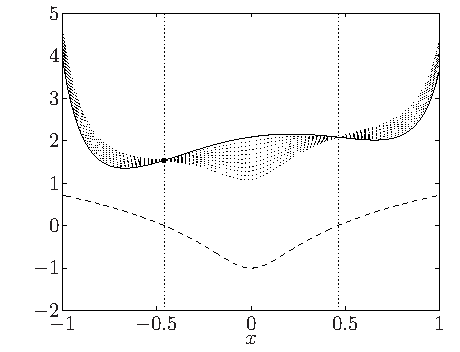
\includegraphics[width=.65\linewidth]{figures/ch05-fig01.pdf}
\caption*{图5.1\quad 对偶可行点给出的下界。实线表示目标函数 $f_0$，虚线表示约束函数 $f_1$。可行集是区间 $[-0.46,0.46]$，由两条点状竖线标出。最优点和最优值为 $x^\star=-0.46$、$p^\star=1.54$（以圆圈表示）。点线曲线表示 $\lambda=0.1,0.2,\ldots,1.0$ 时的 $L(x,\lambda)$。每条曲线的最小值都小于 $p^\star$，因为在可行集上（且 $\lambda\ge0$ 时），有 $L(x,\lambda)\le f_0(x)$。}
\end{figure}
\begin{figure}[htbp]\centering
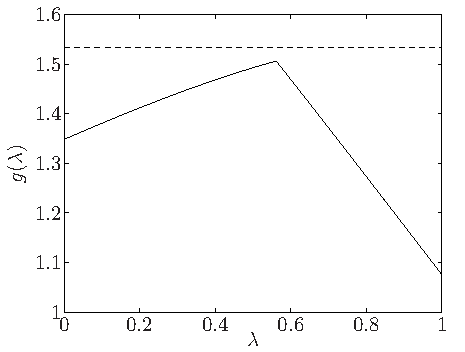
\includegraphics[width=.65\linewidth]{figures/ch05-fig02.pdf}
\caption*{图5.2\quad 图5.1中问题的对偶函数 $g$。虽然 $f_0$ 和 $f_1$ 都不是凸函数，但对偶函数是凹的。水平虚线表示问题的最优值 $p^\star$。}
\end{figure}

% Source PDF page 232 (printed p. 218)
首先把原问题（5.1）改写为无约束问题
\begin{equation}
\text{最小化}\quad f_0(x)+\sum_{i=1}^m I_-(f_i(x))
+\sum_{i=1}^p I_0(h_i(x)),\tag{5.3}
\end{equation}
其中 $I_-:\R\to\R$ 是非正实数集的示性函数，
\[
I_-(u)=\begin{cases}0&u\le0,\\ \infty&u>0,\end{cases}
\]
类似地，$I_0$ 是 $\{0\}$ 的示性函数。在表述（5.3）中，函数 $I_-(u)$ 可以理解为我们对约束函数值 $u=f_i(x)$ 的不满程度：若 $f_i(x)\le0$，不满为零；若 $f_i(x)>0$，不满为无穷大。同样，$I_0(u)$ 给出对等式约束值 $u=h_i(x)$ 的不满程度。可以把 $I_-$ 看作一道“砖墙”，或“无限硬”的不满函数：当 $f_i(x)$ 从非正变为正时，不满程度由零跃升至无穷大。

现在假设在（5.3）中，用线性函数 $\lambda_i u$（$\lambda_i\ge0$）代替 $I_-(u)$，用 $\nu_i u$ 代替 $I_0(u)$。目标就变成拉格朗日函数 $L(x,\lambda,\nu)$，对偶函数值 $g(\lambda,\nu)$ 是以下问题的最优值：
\begin{equation}
\text{最小化}\quad L(x,\lambda,\nu)=f_0(x)+\sum_{i=1}^m\lambda_i f_i(x)
+\sum_{i=1}^p\nu_i h_i(x).\tag{5.4}
\end{equation}
在这种表述中，我们用线性或“软”的不满函数代替 $I_-$ 和 $I_0$。对于不等式约束，当 $f_i(x)=0$ 时不满为零，而当 $f_i(x)>0$ 时不满为正（假设 $\lambda_i>0$）；约束违反得越多，不满程度就越大。在原来的表述中，$f_i(x)$ 的任意非正值都可以接受；在软表述中，有余量的约束，即 $f_i(x)<0$，实际上还会使我们感到满意。

显然，用线性函数 $\lambda_i u$ 近似示性函数 $I_-(u)$ 相当粗糙，但这个线性函数至少是示性函数的一个下估计。因为对任意 $u$ 都有 $\lambda_i u\le I_-(u)$ 和 $\nu_i u\le I_0(u)$，所以立即可知，对偶函数给出原问题最优值的一个下界。

用“软”版本代替“硬”约束的思想，在讨论内点法时还会再次出现（§11.2.1）。

\subsection{例子}
本节给出若干可以推导出拉格朗日对偶函数解析表达式的例子。

\subsubsection*{线性方程的最小二乘解}
考虑问题
\begin{equation}
\begin{array}{ll}\text{最小化}&x^\T x\\
\text{约束为}&Ax=b,\end{array}\tag{5.5}
\end{equation}
其中 $A\in\R^{p\times n}$。问题没有不等式约束，有 $p$ 个（线性）等式约束。拉格朗日函数为
$L(x,\nu)=x^\T x+\nu^\T(Ax-b)$，定义域为 $\R^n\times\R^p$。

% Source PDF page 233 (printed p. 219)
对偶函数为 $g(\nu)=\inf_x L(x,\nu)$。由于 $L(x,\nu)$ 是关于 $x$ 的凸二次函数，可由最优性条件
\[
\nabla_xL(x,\nu)=2x+A^\T\nu=0
\]
求得最小点 $x=-(1/2)A^\T\nu$。因此对偶函数为
\[
g(\nu)=L(-(1/2)A^\T\nu,\nu)=-(1/4)\nu^\T AA^\T\nu-b^\T\nu,
\]
这是定义域为 $\R^p$ 的凹二次函数。下界性质（5.2）说明，对于任意 $\nu\in\R^p$，都有
\[
-(1/4)\nu^\T AA^\T\nu-b^\T\nu\le\inf\{x^\T x\mid Ax=b\}.
\]

\subsubsection*{标准形式的线性规划}
考虑标准形式的线性规划
\begin{equation}
\begin{array}{ll}\text{最小化}&c^\T x\\
\text{约束为}&Ax=b\\&x\succeq0,\end{array}\tag{5.6}
\end{equation}
其不等式约束函数为 $f_i(x)=-x_i$，$i=1,\ldots,n$。为构造拉格朗日函数，对 $n$ 个不等式约束引入乘子 $\lambda_i$，对等式约束引入乘子 $\nu_i$，得到
\[
L(x,\lambda,\nu)=c^\T x-\sum_{i=1}^n\lambda_i x_i+\nu^\T(Ax-b)
=-b^\T\nu+(c+A^\T\nu-\lambda)^\T x.
\]
对偶函数为
\[
g(\lambda,\nu)=\inf_xL(x,\lambda,\nu)
=-b^\T\nu+\inf_x(c+A^\T\nu-\lambda)^\T x.
\]
由于线性函数只有在恒为零时才有下界，因此很容易解析地求出上式。除非 $c+A^\T\nu-\lambda=0$，否则 $g(\lambda,\nu)=-\infty$；等式成立时，其值为 $-b^\T\nu$：
\[
g(\lambda,\nu)=\begin{cases}
-b^\T\nu&A^\T\nu-\lambda+c=0,\\
-\infty&\text{其他情形}.
\end{cases}
\]
注意，对偶函数 $g$ 只在 $\R^m\times\R^p$ 的一个真仿射子集上为有限值。以后会看到，这种情况很常见。

下界性质（5.2）只有当 $\lambda,\nu$ 满足 $\lambda\succeq0$ 和 $A^\T\nu-\lambda+c=0$ 时才是非平凡的。这时 $-b^\T\nu$ 就是线性规划（5.6）最优值的下界。

\subsubsection*{二划分问题}
考虑（非凸）问题
\begin{equation}
\begin{array}{ll}\text{最小化}&x^\T Wx\\
\text{约束为}&x_i^2=1,\quad i=1,\ldots,n,\end{array}\tag{5.7}
\end{equation}

% Source PDF page 234 (printed p. 220)
其中 $W\in\mathbf S^n$。约束把 $x_i$ 的取值限制为 $1$ 或 $-1$，所以该问题等价于在所有分量为 $\pm1$ 的向量中，寻找使 $x^\T Wx$ 最小的一个。这里可行集是有限的（包含 $2^n$ 个点），因此原则上可以检查每个可行点的目标值来求解。不过，可行点数呈指数增长，这种方法仅适用于小问题（例如 $n\le30$）。一般而言（例如 $n$ 大于50时），问题（5.7）非常难解。

可将（5.7）解释为 $n$ 个元素（如 $\{1,\ldots,n\}$）的二划分问题：可行向量 $x$ 对应于划分
\[
\{1,\ldots,n\}=\{i\mid x_i=-1\}\cup\{i\mid x_i=1\}.
\]
矩阵系数 $W_{ij}$ 可以理解为将元素 $i,j$ 放在同一组的代价，$-W_{ij}$ 则是将二者放在不同组的代价。（5.7）的目标是对所有元素对求和得到的总代价，问题就是寻找总代价最小的划分。

现在推导其对偶函数。拉格朗日函数为
\begin{align*}
L(x,\nu)&=x^\T Wx+\sum_{i=1}^n\nu_i(x_i^2-1)\\
&=x^\T(W+\diag(\nu))x-\one^\T\nu.
\end{align*}
对 $x$ 最小化，得到拉格朗日对偶函数
\[
g(\nu)=\inf_x x^\T(W+\diag(\nu))x-\one^\T\nu
=\begin{cases}-\one^\T\nu&W+\diag(\nu)\succeq0,\\
-\infty&\text{其他情形},\end{cases}
\]
这里利用了二次型的下确界要么为零（当其半正定时），要么为 $-\infty$（当其非半正定时）。

这一对偶函数给出难解问题（5.7）最优值的下界。例如，可取对偶变量的特定值
\[
\nu=-\lambda_{\min}(W)\one.
\]
它是对偶可行的，因为 $W+\diag(\nu)=W-\lambda_{\min}(W)I\succeq0$。由此得到最优值 $p^\star$ 的界
\begin{equation}
p^\star\ge-\one^\T\nu=n\lambda_{\min}(W).\tag{5.8}
\end{equation}

\paragraph{注5.1}
也可以不借助拉格朗日对偶函数来得到这个下界。首先，用 $\sum_{i=1}^n x_i^2=n$ 代替约束 $x_1^2=1,\ldots,x_n^2=1$，得到修改后的问题
\begin{equation}
\begin{array}{ll}\text{最小化}&x^\T Wx\\
\text{约束为}&\sum_{i=1}^n x_i^2=n.\end{array}\tag{5.9}
\end{equation}

% Source PDF page 235 (printed p. 221)
原问题（5.7）的约束蕴含这里的约束，因此问题（5.9）的最优值是（5.7）最优值 $p^\star$ 的下界。而修改后的问题（5.9）容易作为特征值问题求解，其最优值为 $n\lambda_{\min}(W)$。

\subsection{拉格朗日对偶函数与共轭函数}
回顾§3.3，函数 $f:\R^n\to\R$ 的共轭 $f^*$ 为
\[
f^*(y)=\sup_{x\in\dom f}\bigl(y^\T x-f(x)\bigr).
\]
共轭函数与拉格朗日对偶函数密切相关。为说明一个简单联系，考虑问题
\[
\begin{array}{ll}\text{最小化}&f(x)\\\text{约束为}&x=0.\end{array}
\]
（这一问题并不十分有趣，观察即可求解。）其拉格朗日函数为 $L(x,\nu)=f(x)+\nu^\T x$，对偶函数为
\[
g(\nu)=\inf_x(f(x)+\nu^\T x)
=-\sup_x\bigl((-\nu)^\T x-f(x)\bigr)=-f^*(-\nu).
\]

更一般地（也更有用地），考虑带线性不等式和等式约束的优化问题
\begin{equation}
\begin{array}{ll}\text{最小化}&f_0(x)\\
\text{约束为}&Ax\preceq b\\&Cx=d.\end{array}\tag{5.10}
\end{equation}
利用 $f_0$ 的共轭，可将（5.10）的对偶函数写为
\begin{align}
g(\lambda,\nu)
&=\inf_x\bigl(f_0(x)+\lambda^\T(Ax-b)+\nu^\T(Cx-d)\bigr)\notag\\
&=-b^\T\lambda-d^\T\nu+\inf_x\bigl(f_0(x)+(A^\T\lambda+C^\T\nu)^\T x\bigr)\notag\\
&=-b^\T\lambda-d^\T\nu-f_0^*(-A^\T\lambda-C^\T\nu).\tag{5.11}
\end{align}
$g$ 的定义域可由 $f_0^*$ 的定义域得出：
\[
\dom g=\{(\lambda,\nu)\mid -A^\T\lambda-C^\T\nu\in\dom f_0^*\}.
\]
下面用几个例子说明。

\subsubsection*{等式约束范数最小化}
考虑问题
\begin{equation}
\begin{array}{ll}\text{最小化}&\norm{x}\\
\text{约束为}&Ax=b,\end{array}\tag{5.12}
\end{equation}

% Source PDF page 236 (printed p. 222)
其中 $\norm{\cdot}$ 是任意范数。回顾第93页的例3.26，$f_0=\norm{\cdot}$ 的共轭为
\[
f_0^*(y)=\begin{cases}0&\norm{y}_*\le1,\\
\infty&\text{其他情形},\end{cases}
\]
即对偶范数单位球的示性函数。利用上面的结果（5.11），问题（5.12）的对偶函数为
\[
g(\nu)=-b^\T\nu-f_0^*(-A^\T\nu)
=\begin{cases}-b^\T\nu&\norm{A^\T\nu}_*\le1,\\
-\infty&\text{其他情形}.\end{cases}
\]

\subsubsection*{熵最大化}
考虑熵最大化问题
\begin{equation}
\begin{array}{ll}\text{最小化}&f_0(x)=\sum_{i=1}^n x_i\log x_i\\
\text{约束为}&Ax\preceq b\\&\one^\T x=1,\end{array}\tag{5.13}
\end{equation}
其中 $\dom f_0=\R_{++}^n$。标量变量 $u$ 的负熵函数 $u\log u$ 的共轭为 $e^{v-1}$（见第91页例3.21）。由于 $f_0$ 是不同变量的负熵函数之和，可知其共轭为
\[
f_0^*(y)=\sum_{i=1}^n e^{y_i-1},\qquad \dom f_0^*=\R^n.
\]
利用结果（5.11），（5.13）的对偶函数为
\[
g(\lambda,\nu)=-b^\T\lambda-\nu-\sum_{i=1}^n e^{-a_i^\T\lambda-\nu-1}
=-b^\T\lambda-\nu-e^{-\nu-1}\sum_{i=1}^n e^{-a_i^\T\lambda},
\]
其中 $a_i$ 是 $A$ 的第 $i$ 列。

\subsubsection*{最小体积覆盖椭球}
考虑变量为 $X\in\mathbf S^n$ 的问题
\begin{equation}
\begin{array}{ll}\text{最小化}&f_0(X)=\log\det X^{-1}\\
\text{约束为}&a_i^\T Xa_i\le1,\quad i=1,\ldots,m,\end{array}\tag{5.14}
\end{equation}
其中 $\dom f_0=\mathbf S_{++}^n$。问题（5.14）有简单的几何解释。每个 $X\in\mathbf S_{++}^n$ 对应一个以原点为中心的椭球
\[
\mathcal E_X=\{z\mid z^\T Xz\le1\}.
\]
这个椭球的体积与 $(\det X^{-1})^{1/2}$ 成正比，所以除去一个常数和一个二倍因子，（5.14）的目标就是椭球体积的对数。

% Source PDF page 237 (printed p. 223)
问题（5.14）的约束要求 $a_i\in\mathcal E_X$。因此，它寻找包含点 $a_1,\ldots,a_m$、以原点为中心的最小体积椭球。

问题（5.14）的不等式约束是仿射的，可写为 $\tr((a_i a_i^\T)X)\le1$。在第92页例3.23中，已求得 $f_0$ 的共轭为
\[
f_0^*(Y)=\log\det(-Y)^{-1}-n,\qquad \dom f_0^*=-\mathbf S_{++}^n.
\]
利用结果（5.11），问题（5.14）的对偶函数为
\begin{equation}
g(\lambda)=\begin{cases}
\log\det\left(\sum_{i=1}^m\lambda_i a_i a_i^\T\right)-\one^\T\lambda+n
&\sum_{i=1}^m\lambda_i a_i a_i^\T\succ0,\\
-\infty&\text{其他情形}.
\end{cases}\tag{5.15}
\end{equation}
因此，对于任意满足 $\lambda\succeq0$、$\sum_{i=1}^m\lambda_i a_i a_i^\T\succ0$ 的 $\lambda$，
\[
\log\det\left(\sum_{i=1}^m\lambda_i a_i a_i^\T\right)-\one^\T\lambda+n
\]
都是问题（5.14）最优值的一个下界。

\section{拉格朗日对偶问题}
对于每个满足 $\lambda\succeq0$ 的 $(\lambda,\nu)$，拉格朗日对偶函数都给出优化问题（5.1）最优值 $p^\star$ 的一个下界。这样就有了一个依赖参数 $\lambda,\nu$ 的下界。自然要问：从拉格朗日对偶函数出发，能得到的最佳下界是什么？

由此得到优化问题
\begin{equation}
\begin{array}{ll}\text{最大化}&g(\lambda,\nu)\\
\text{约束为}&\lambda\succeq0.\end{array}\tag{5.16}
\end{equation}
这一问题称为问题（5.1）的\emph{拉格朗日对偶问题}。在这一语境中，原来的问题（5.1）有时称为\emph{原始问题}。现在，用“对偶可行”来描述满足 $\lambda\succeq0$ 和 $g(\lambda,\nu)>-\infty$ 的 $(\lambda,\nu)$ 就顺理成章了：它表示 $(\lambda,\nu)$ 是对偶问题（5.16）的可行点。若 $(\lambda^\star,\nu^\star)$ 是（5.16）的最优解，就称其为\emph{对偶最优解}或\emph{最优拉格朗日乘子}。

拉格朗日对偶问题（5.16）是凸优化问题，因为要最大化的目标是凹函数，约束也是凸的。无论原始问题（5.1）是否凸，这一点都成立。

% Source PDF page 238 (printed p. 224)
\subsection{显式写出对偶约束}
上面的例子说明，对偶函数的定义域
\[
\dom g=\{(\lambda,\nu)\mid g(\lambda,\nu)>-\infty\}
\]
的维数小于 $m+p$ 并不少见。许多情况下，可以确定 $\dom g$ 的仿射包，并把它描述为一组线性等式约束。粗略地说，就是可以识别出“隐藏”或“隐含”在对偶问题（5.16）目标 $g$ 中的等式约束。这时可以构造一个等价问题，将这些等式明确地列为约束。下面的例子说明这一思想。

\subsubsection*{标准形式线性规划的拉格朗日对偶}
第219页已求得标准形式线性规划
\begin{equation}
\begin{array}{ll}\text{最小化}&c^\T x\\
\text{约束为}&Ax=b\\&x\succeq0\end{array}\tag{5.17}
\end{equation}
的拉格朗日对偶函数为
\[
g(\lambda,\nu)=\begin{cases}-b^\T\nu&A^\T\nu-\lambda+c=0,\\
-\infty&\text{其他情形}.\end{cases}
\]
严格地说，标准形式线性规划的拉格朗日对偶问题是在 $\lambda\succeq0$ 上最大化上述 $g$，即
\begin{equation}
\begin{array}{ll}
\text{最大化}&g(\lambda,\nu)=
\begin{cases}-b^\T\nu&A^\T\nu-\lambda+c=0,\\-\infty&\text{其他情形}\end{cases}\\
\text{约束为}&\lambda\succeq0.
\end{array}\tag{5.18}
\end{equation}
只有当 $A^\T\nu-\lambda+c=0$ 时，$g$ 才是有限的。将这些等式约束显式写出，可得等价问题
\begin{equation}
\begin{array}{ll}\text{最大化}&-b^\T\nu\\
\text{约束为}&A^\T\nu-\lambda+c=0\\&\lambda\succeq0.\end{array}\tag{5.19}
\end{equation}
它又可表示为
\begin{equation}
\begin{array}{ll}\text{最大化}&-b^\T\nu\\
\text{约束为}&A^\T\nu+c\succeq0,\end{array}\tag{5.20}
\end{equation}
这是不等式形式的线性规划。

注意这三个问题之间的细微区别。标准形式线性规划（5.17）的拉格朗日对偶是（5.18），它与（5.19）、（5.20）等价，却并非同一个问题。稍微放宽术语，我们也将（5.19）或（5.20）称为标准形式线性规划（5.17）的拉格朗日对偶。

% Source PDF page 239 (printed p. 225)
\subsubsection*{不等式形式线性规划的拉格朗日对偶}
类似地，可以求出不等式形式线性规划
\begin{equation}
\begin{array}{ll}\text{最小化}&c^\T x\\\text{约束为}&Ax\preceq b\end{array}\tag{5.21}
\end{equation}
的拉格朗日对偶问题。拉格朗日函数为
\[
L(x,\lambda)=c^\T x+\lambda^\T(Ax-b)
=-b^\T\lambda+(A^\T\lambda+c)^\T x,
\]
所以对偶函数为
\[
g(\lambda)=\inf_x L(x,\lambda)
=-b^\T\lambda+\inf_x(A^\T\lambda+c)^\T x.
\]
线性函数的下确界为 $-\infty$，唯一例外是它恒为零。因此对偶函数为
\[
g(\lambda)=\begin{cases}
-b^\T\lambda&A^\T\lambda+c=0,\\
-\infty&\text{其他情形}.
\end{cases}
\]
若 $\lambda\succeq0$ 且 $A^\T\lambda+c=0$，则对偶变量 $\lambda$ 对偶可行。

线性规划（5.21）的拉格朗日对偶是在所有 $\lambda\succeq0$ 上最大化 $g$。同样，把对偶可行条件显式列为约束，就可改写为
\begin{equation}
\begin{array}{ll}\text{最大化}&-b^\T\lambda\\
\text{约束为}&A^\T\lambda+c=0\\&\lambda\succeq0,\end{array}\tag{5.22}
\end{equation}
这是一个标准形式的线性规划。

标准形式与不等式形式的线性规划及其对偶之间存在有趣的对称性：标准形式线性规划的对偶是仅含不等式约束的线性规划，反之亦然。还可验证，（5.22）的拉格朗日对偶与原始问题（5.21）等价。

\subsection{弱对偶}
拉格朗日对偶问题的最优值记为 $d^\star$。按定义，它是从拉格朗日对偶函数能得到的 $p^\star$ 的最佳下界。特别地，有简单而重要的不等式
\begin{equation}
d^\star\le p^\star,\tag{5.23}
\end{equation}
即使原问题非凸，这一不等式也成立。该性质称为\emph{弱对偶}。

当 $d^\star,p^\star$ 是无穷值时，弱对偶不等式（5.23）也成立。例如，若原始问题无下界，即 $p^\star=-\infty$，则必有 $d^\star=-\infty$，也就是说拉格朗日对偶问题不可行。反之，若对偶问题无上界，即 $d^\star=\infty$，则必有 $p^\star=\infty$，也就是说原始问题不可行。

% Source PDF page 240 (printed p. 226)
称差值 $p^\star-d^\star$ 为原问题的\emph{最优对偶间隙}，因为它给出原始问题最优值与拉格朗日对偶函数能够提供的最佳（即最大）下界之间的差距。最优对偶间隙总是非负的。

由于对偶问题总是凸的，许多情况下可高效求解出 $d^\star$，因此有时可以利用（5.23）为一个难解问题的最优值求下界。例如，考虑第219页的二划分问题（5.7）。它的对偶问题是半正定规划
\[
\begin{array}{ll}\text{最大化}&-\one^\T\nu\\
\text{约束为}&W+\diag(\nu)\succeq0,\end{array}
\]
变量为 $\nu\in\R^n$。即使 $n$ 相当大，例如 $n=1000$，也能高效求解这个问题。其最优值是二划分问题最优值的下界，而且至少与基于 $\lambda_{\min}(W)$ 的下界（5.8）一样好。

\subsection{强对偶与Slater约束资格}
若等式
\begin{equation}
d^\star=p^\star\tag{5.24}
\end{equation}
成立，即最优对偶间隙为零，则称\emph{强对偶}成立。这意味着从拉格朗日对偶函数能够得到的最佳下界是紧的。

一般而言，强对偶未必成立。不过，若原始问题（5.1）是凸的，即具有形式
\begin{equation}
\begin{array}{ll}\text{最小化}&f_0(x)\\
\text{约束为}&f_i(x)\le0,\quad i=1,\ldots,m\\&Ax=b,\end{array}\tag{5.25}
\end{equation}
其中 $f_0,\ldots,f_m$ 凸，则通常（但并非总是）有强对偶。有许多结果给出除凸性以外还能保证强对偶的条件，这些条件称为\emph{约束资格}。

一个简单的约束资格是\emph{Slater条件}：存在 $x\in\relint D$，使得
\begin{equation}
f_i(x)<0,\quad i=1,\ldots,m,\qquad Ax=b.\tag{5.26}
\end{equation}
这样的点有时称为\emph{严格可行点}，因为不等式约束都严格成立。Slater定理说明，若Slater条件成立（且问题凸），则强对偶成立。

若某些不等式约束函数 $f_i$ 是仿射的，Slater条件还可放宽。若前 $k$ 个约束函数 $f_1,\ldots,f_k$ 仿射，那么只要满足以下较弱条件，强对偶就成立：存在 $x\in\relint D$，满足
\begin{equation}
\begin{gathered}
f_i(x)\le0,\quad i=1,\ldots,k,\qquad
f_i(x)<0,\quad i=k+1,\ldots,m,\\
Ax=b.
\end{gathered}\tag{5.27}
\end{equation}

% Source PDF page 241 (printed p. 227)
换言之，仿射不等式不必严格成立。注意，当约束全为线性等式和不等式，且 $\dom f_0$ 是开集时，放宽的Slater条件（5.27）就简化为可行性。

Slater条件（以及放宽的条件（5.27））不仅蕴含凸问题的强对偶，还蕴含当 $d^\star>-\infty$ 时，对偶最优值能够达到。也就是说，存在对偶可行的 $(\lambda^\star,\nu^\star)$，满足 $g(\lambda^\star,\nu^\star)=d^\star=p^\star$。§5.3.2将证明：当原始问题凸且Slater条件成立时，强对偶成立。

\subsection{例子}
\subsubsection*{线性方程的最小二乘解}
回顾问题（5.5）：
\[
\begin{array}{ll}\text{最小化}&x^\T x\\\text{约束为}&Ax=b.\end{array}
\]
相应对偶问题为
\[
\text{最大化}\quad -(1/4)\nu^\T AA^\T\nu-b^\T\nu,
\]
这是无约束的凹二次最大化问题。

Slater条件仅要求原始问题可行，因此只要 $b\in\mathcal R(A)$，即 $p^\star<\infty$，就有 $p^\star=d^\star$。事实上，这个问题总有强对偶，即使 $p^\star=\infty$ 也如此。当 $b\notin\mathcal R(A)$ 时，存在 $z$ 使 $A^\T z=0$、$b^\T z\ne0$。因此对偶函数沿直线 $\{tz\mid t\in\R\}$ 无上界，从而也有 $d^\star=\infty$。

\subsubsection*{线性规划的拉格朗日对偶}
根据较弱的Slater条件，只要原始问题可行，任意线性规划（标准形式或不等式形式）都有强对偶。对其对偶问题也应用这个结果，可知只要对偶可行，线性规划也有强对偶。因此，线性规划强对偶可能失败的情况只剩一种：原始问题和对偶问题都不可行。这种病态情形确实可能发生，见习题5.23。

\subsubsection*{QCQP的拉格朗日对偶}
考虑二次约束二次规划
\begin{equation}
\begin{array}{ll}\text{最小化}&(1/2)x^\T P_0x+q_0^\T x+r_0\\
\text{约束为}&(1/2)x^\T P_ix+q_i^\T x+r_i\le0,\quad i=1,\ldots,m,\end{array}\tag{5.28}
\end{equation}
其中 $P_0\in\mathbf S_{++}^n$，$P_i\in\mathbf S_+^n$，$i=1,\ldots,m$。拉格朗日函数为
\[
L(x,\lambda)=(1/2)x^\T P(\lambda)x+q(\lambda)^\T x+r(\lambda),
\]
其中
\[
P(\lambda)=P_0+\sum_{i=1}^m\lambda_i P_i,\quad
q(\lambda)=q_0+\sum_{i=1}^m\lambda_i q_i,\quad
r(\lambda)=r_0+\sum_{i=1}^m\lambda_i r_i.
\]

% Source PDF page 242 (printed p. 228)
对于一般的 $\lambda$，可以求出 $g(\lambda)$ 的表达式，但相当复杂。不过，若 $\lambda\succeq0$，则 $P(\lambda)\succ0$，而且
\[
g(\lambda)=\inf_x L(x,\lambda)
=-(1/2)q(\lambda)^\T P(\lambda)^{-1}q(\lambda)+r(\lambda).
\]
因此，对偶问题可写为
\begin{equation}
\begin{array}{ll}\text{最大化}&-(1/2)q(\lambda)^\T P(\lambda)^{-1}q(\lambda)+r(\lambda)\\
\text{约束为}&\lambda\succeq0.\end{array}\tag{5.29}
\end{equation}
Slater条件说明，若二次不等式约束严格可行，即存在 $x$ 满足
\[
(1/2)x^\T P_ix+q_i^\T x+r_i<0,\quad i=1,\ldots,m,
\]
则（5.29）与（5.28）之间强对偶成立。

\subsubsection*{熵最大化}
下一个例子是熵最大化问题（5.13）：
\[
\begin{array}{ll}\text{最小化}&\sum_{i=1}^n x_i\log x_i\\
\text{约束为}&Ax\preceq b\\&\one^\T x=1,\end{array}
\]
定义域为 $D=\R_+^n$。第222页已求得拉格朗日对偶函数；对偶问题为
\begin{equation}
\begin{array}{ll}
\text{最大化}&-b^\T\lambda-\nu-e^{-\nu-1}\sum_{i=1}^n e^{-a_i^\T\lambda}\\
\text{约束为}&\lambda\succeq0,\end{array}\tag{5.30}
\end{equation}
变量为 $\lambda\in\R^m$、$\nu\in\R$。（5.13）的较弱Slater条件说明，若存在满足 $Ax\preceq b$、$\one^\T x=1$ 的 $x\succ0$，则最优对偶间隙为零。

可以对对偶变量 $\nu$ 解析地最大化，从而简化（5.30）。固定 $\lambda$ 后，目标在关于 $\nu$ 的导数为零时取得最大值，即
\[
\nu=\log\left(\sum_{i=1}^n e^{-a_i^\T\lambda}\right)-1.
\]
把这一 $\nu$ 的最优值代回对偶问题，得到
\[
\begin{array}{ll}
\text{最大化}&-b^\T\lambda-\log\left(\sum_{i=1}^n e^{-a_i^\T\lambda}\right)\\
\text{约束为}&\lambda\succeq0,\end{array}
\]
这是带非负约束的几何规划（凸形式）。

\subsubsection*{最小体积覆盖椭球}
考虑问题（5.14）：
\[
\begin{array}{ll}\text{最小化}&\log\det X^{-1}\\
\text{约束为}&a_i^\T Xa_i\le1,\quad i=1,\ldots,m,\end{array}
\]

% Source PDF page 243 (printed p. 229)
其定义域为 $D=\mathbf S_{++}^n$。拉格朗日对偶函数由（5.15）给出，所以对偶问题可表示为
\begin{equation}
\begin{array}{ll}\text{最大化}&
\log\det\left(\sum_{i=1}^m\lambda_i a_i a_i^\T\right)-\one^\T\lambda+n\\
\text{约束为}&\lambda\succeq0,\end{array}\tag{5.31}
\end{equation}
其中约定当 $X\not\succ0$ 时 $\log\det X=-\infty$。

问题（5.14）的较弱Slater条件要求，存在 $X\in\mathbf S_{++}^n$，使 $a_i^\T Xa_i\le1$，$i=1,\ldots,m$。这一条件总是满足，因此（5.14）与对偶问题（5.31）之间总有强对偶。

\subsubsection*{具有强对偶的非凸二次问题}
在少数情况下，非凸问题也有强对偶。一个重要例子是在单位球上最小化非凸二次函数：
\begin{equation}
\begin{array}{ll}\text{最小化}&x^\T Ax+2b^\T x\\
\text{约束为}&x^\T x\le1,\end{array}\tag{5.32}
\end{equation}
其中 $A\in\mathbf S^n$、$A\not\succeq0$、$b\in\R^n$。由于 $A\not\succeq0$，这不是凸问题。它有时称为\emph{信赖域问题}，出现在单位球上最小化一个函数的二阶近似时；假设该近似在这个区域内大致有效。

拉格朗日函数为
\[
L(x,\lambda)=x^\T Ax+2b^\T x+\lambda(x^\T x-1)
=x^\T(A+\lambda I)x+2b^\T x-\lambda,
\]
所以对偶函数为
\[
g(\lambda)=\begin{cases}
-b^\T(A+\lambda I)^\dagger b-\lambda&
A+\lambda I\succeq0,\quad b\in\mathcal R(A+\lambda I),\\
-\infty&\text{其他情形},
\end{cases}
\]
其中 $(A+\lambda I)^\dagger$ 为 $A+\lambda I$ 的伪逆。因此拉格朗日对偶问题为
\begin{equation}
\begin{array}{ll}\text{最大化}&-b^\T(A+\lambda I)^\dagger b-\lambda\\
\text{约束为}&A+\lambda I\succeq0,\quad b\in\mathcal R(A+\lambda I),\end{array}\tag{5.33}
\end{equation}
变量为 $\lambda\in\R$。虽然从这个表达式看不明显，但它确实是凸优化问题。事实上，它容易求解，因为可写为
\[
\begin{array}{ll}\text{最大化}&-\sum_{i=1}^n(q_i^\T b)^2/(\lambda_i+\lambda)-\lambda\\
\text{约束为}&\lambda\ge-\lambda_{\min}(A),\end{array}
\]
其中 $\lambda_i$、$q_i$ 是 $A$ 的特征值和相应（标准正交）特征向量；当 $q_i^\T b=0$ 时，将 $(q_i^\T b)^2/0$ 解释为 $0$，其他情况下解释为 $\infty$。

虽然原问题（5.32）非凸，但它的最优对偶间隙总为零：（5.32）与（5.33）的最优值总相同。事实上，更一般的结论成立：任意目标为二次函数、只有一个二次不等式约束的优化问题，只要Slater条件成立，就有强对偶，见§B.1。

% Source PDF page 244 (printed p. 230)
\subsection{矩阵博弈的混合策略}
本节用强对偶推导零和矩阵博弈的一个基本结果。考虑两位参与者的博弈。参与者1选择（或行动）$k\in\{1,\ldots,n\}$，参与者2选择 $l\in\{1,\ldots,m\}$。随后参与者1向参与者2支付 $P_{kl}$，其中 $P\in\R^{n\times m}$ 为博弈的\emph{支付矩阵}。参与者1的目标是使支付尽可能小，参与者2的目标则是使其尽可能大。

参与者采用\emph{随机化策略}或\emph{混合策略}，即各自按照某个概率分布随机选择，且双方的选择相互独立：
\[
\operatorname{prob}(k=i)=u_i,\quad i=1,\ldots,n,\qquad
\operatorname{prob}(l=i)=v_i,\quad i=1,\ldots,m.
\]
这里 $u,v$ 给出双方选择的概率分布，也就是相应策略。于是参与者1向参与者2的期望支付为
\[
\sum_{k=1}^n\sum_{l=1}^m u_kv_lP_{kl}=u^\T Pv.
\]
参与者1希望选择 $u$ 使 $u^\T Pv$ 最小；参与者2希望选择 $v$ 使其最大。

先从参与者1的角度分析，假设参与者2知道她的策略 $u$（这显然使参与者2占优）。参与者2会选择 $v$ 使 $u^\T Pv$ 最大，得到期望支付
\[
\sup\{u^\T Pv\mid v\succeq0,\ \one^\T v=1\}
=\max_{i=1,\ldots,m}(P^\T u)_i.
\]
参与者1能做的最好选择，就是选取 $u$ 使这一最坏情况下向参与者2的支付最小，即选择求解以下问题的策略：
\begin{equation}
\begin{array}{ll}\text{最小化}&\max_{i=1,\ldots,m}(P^\T u)_i\\
\text{约束为}&u\succeq0,\quad\one^\T u=1,\end{array}\tag{5.34}
\end{equation}
这是分段线性的凸优化问题。以 $p_1^\star$ 记其最优值。它是在参与者2知道参与者1的策略、并采取对自己最有利行动的情况下，参与者1能安排的最小期望支付。

类似地，可以考虑参与者1知道参与者2策略 $v$ 的情形（这使参与者1占优）。此时参与者1选择 $u$ 使 $u^\T Pv$ 最小，得到期望支付
\[
\inf\{u^\T Pv\mid u\succeq0,\ \one^\T u=1\}
=\min_{i=1,\ldots,n}(Pv)_i.
\]
参与者2选择 $v$ 使这一数值最大，即选择求解以下问题的策略：
\begin{equation}
\begin{array}{ll}\text{最大化}&\min_{i=1,\ldots,n}(Pv)_i\\
\text{约束为}&v\succeq0,\quad\one^\T v=1,\end{array}\tag{5.35}
\end{equation}

% Source PDF page 245 (printed p. 231)
这也是凸优化问题，其目标是分段线性（凹）函数。以 $p_2^\star$ 记其最优值。它是在参与者1知道参与者2策略的情况下，参与者2能够保证得到的最大期望支付。

直观上，知道对手策略会带来优势（至少不会有害）；而且容易证明，总有 $p_1^\star\ge p_2^\star$。非负差值 $p_1^\star-p_2^\star$ 可以理解为知道对手策略给参与者带来的优势。

利用对偶，可以得到初看令人意外的结果：$p_1^\star=p_2^\star$。换言之，在采用混合策略的矩阵博弈中，知道对手策略并不带来优势。下面通过说明（5.34）与（5.35）互为拉格朗日对偶、且强对偶成立，来证明这个结果。

先将（5.34）写成线性规划
\[
\begin{array}{ll}\text{最小化}&t\\
\text{约束为}&u\succeq0,\quad\one^\T u=1\\
&P^\T u\preceq t\one,\end{array}
\]
其中引入额外变量 $t\in\R$。对 $P^\T u\preceq t\one$ 引入乘子 $\lambda$，对 $u\succeq0$ 引入 $\mu$，对 $\one^\T u=1$ 引入 $\nu$，得到拉格朗日函数
\[
\begin{aligned}
&t+\lambda^\T(P^\T u-t\one)-\mu^\T u+\nu(1-\one^\T u)\\
&\qquad=\nu+(1-\one^\T\lambda)t+(P\lambda-\nu\one-\mu)^\T u.
\end{aligned}
\]
因此对偶函数为
\[
g(\lambda,\mu,\nu)=\begin{cases}
\nu&\one^\T\lambda=1,\quad P\lambda-\nu\one=\mu,\\
-\infty&\text{其他情形}.
\end{cases}
\]
于是对偶问题为
\[
\begin{array}{ll}\text{最大化}&\nu\\
\text{约束为}&\lambda\succeq0,\quad\one^\T\lambda=1,\quad\mu\succeq0\\
&P\lambda-\nu\one=\mu.\end{array}
\]
消去 $\mu$，得到（5.34）的拉格朗日对偶
\[
\begin{array}{ll}\text{最大化}&\nu\\
\text{约束为}&\lambda\succeq0,\quad\one^\T\lambda=1\\
&P\lambda\succeq\nu\one,\end{array}
\]
变量为 $\lambda,\nu$。它显然与（5.35）等价。由于这些线性规划可行，强对偶成立；（5.34）与（5.35）的最优值相等。

% Source PDF page 246 (printed p. 232)
\section{几何解释}
\subsection{通过值集解释弱对偶与强对偶}
利用集合
\begin{equation}
\begin{split}
\mathcal G=\{&(f_1(x),\ldots,f_m(x),h_1(x),\ldots,h_p(x),f_0(x))\\
&\in\R^m\times\R^p\times\R\mid x\in D\},
\end{split}\tag{5.36}
\end{equation}
可以给对偶函数一个简单的几何解释。$\mathcal G$ 是约束函数和目标函数所取值组成的集合。问题（5.1）的最优值容易用 $\mathcal G$ 写成
\[
p^\star=\inf\{t\mid(u,v,t)\in\mathcal G,\ u\preceq0,\ v=0\}.
\]
为计算 $(\lambda,\nu)$ 处的对偶函数值，只需在 $(u,v,t)\in\mathcal G$ 上最小化仿射函数
\[
(\lambda,\nu,1)^\T(u,v,t)=\sum_{i=1}^m\lambda_i u_i+\sum_{i=1}^p\nu_i v_i+t,
\]
即
\[
g(\lambda,\nu)=\inf\{(\lambda,\nu,1)^\T(u,v,t)\mid(u,v,t)\in\mathcal G\}.
\]
特别地，若下确界有限，则不等式
\[
(\lambda,\nu,1)^\T(u,v,t)\ge g(\lambda,\nu)
\]
确定 $\mathcal G$ 的一个支撑超平面。有时称它为\emph{非竖直}支撑超平面，因为其法向量的最后一个分量非零。

现在设 $\lambda\succeq0$。显然，当 $u\preceq0$、$v=0$ 时，
$t\ge(\lambda,\nu,1)^\T(u,v,t)$。因此
\[
\begin{aligned}
p^\star&=\inf\{t\mid(u,v,t)\in\mathcal G,\ u\preceq0,\ v=0\}\\
&\ge\inf\{(\lambda,\nu,1)^\T(u,v,t)\mid(u,v,t)\in\mathcal G,\ u\preceq0,\ v=0\}\\
&\ge\inf\{(\lambda,\nu,1)^\T(u,v,t)\mid(u,v,t)\in\mathcal G\}\\
&=g(\lambda,\nu),
\end{aligned}
\]
这就是弱对偶。图5.3和图5.4用一个只有一个不等式约束的简单问题说明这一解释。

\subsubsection*{上图形式的变体}
本节给出基于 $\mathcal G$ 的对偶几何解释的一个变体，它能说明为什么（大多数）凸问题具有强对偶。定义集合 $\mathcal A\subseteq\R^m\times\R^p\times\R$ 为
\begin{equation}
\mathcal A=\mathcal G+\bigl(\R_+^m\times\{0\}\times\R_+\bigr),\tag{5.37}
\end{equation}
更显式地，
\[
\begin{split}
\mathcal A=\{(u,v,t)\mid{}&\exists x\in D,\ f_i(x)\le u_i,\quad i=1,\ldots,m,\\
&h_i(x)=v_i,\quad i=1,\ldots,p,\quad f_0(x)\le t\}.
\end{split}
\]

% Source PDF page 247 (printed p. 233)
\begin{figure}[htbp]\centering
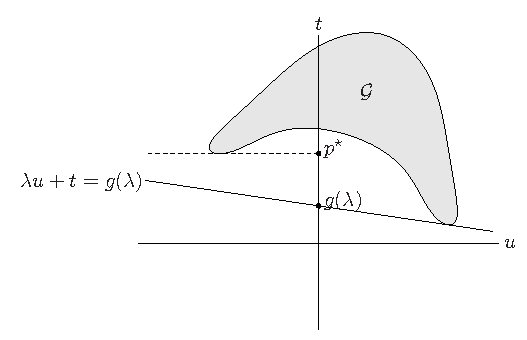
\includegraphics[width=.7\linewidth]{figures/ch05-fig03.pdf}
\caption*{图5.3\quad 对偶函数及下界 $g(\lambda)\le p^\star$ 的几何解释，所示问题含一个（不等式）约束。给定 $\lambda$，在 $\mathcal G=\{(f_1(x),f_0(x))\mid x\in D\}$ 上最小化 $(\lambda,1)^\T(u,t)$，得到斜率为 $-\lambda$ 的支撑超平面。该超平面与 $u=0$ 轴的交点给出 $g(\lambda)$。}
\end{figure}
\begin{figure}[htbp]\centering
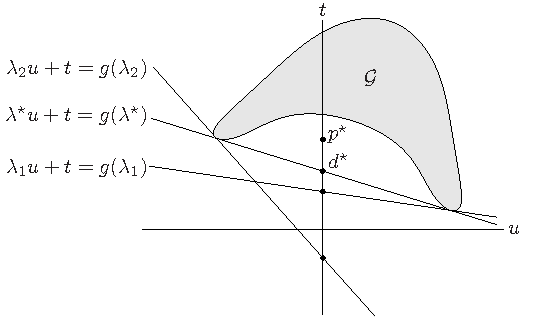
\includegraphics[width=.7\linewidth]{figures/ch05-fig04.pdf}
\caption*{图5.4\quad 三个对偶可行 $\lambda$ 值所对应的支撑超平面，其中包括最优值 $\lambda^\star$。强对偶不成立；最优对偶间隙 $p^\star-d^\star$ 为正。}
\end{figure}

% Source PDF page 248 (printed p. 234)
\begin{figure}[htbp]\centering
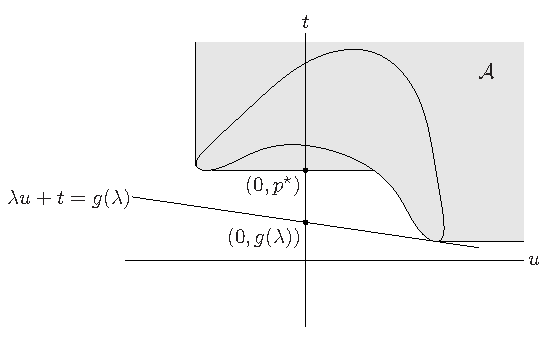
\includegraphics[width=.7\linewidth]{figures/ch05-fig05.pdf}
\caption*{图5.5\quad 对偶函数及下界 $g(\lambda)\le p^\star$ 的几何解释，所示问题含一个（不等式）约束。给定 $\lambda$，在 $\mathcal A=\{(u,t)\mid\exists x\in D,\ f_0(x)\le t,\ f_1(x)\le u\}$ 上最小化 $(\lambda,1)^\T(u,t)$，得到斜率为 $-\lambda$ 的支撑超平面。该超平面与 $u=0$ 轴的交点给出 $g(\lambda)$。}
\end{figure}
可以把 $\mathcal A$ 看作 $\mathcal G$ 的某种上图形式，因为 $\mathcal A$ 包含 $\mathcal G$ 的所有点，也包含“更差”的点，即目标值或不等式约束函数值更大的点。

最优值可用 $\mathcal A$ 表示为
\[
p^\star=\inf\{t\mid(0,0,t)\in\mathcal A\}.
\]
在满足 $\lambda\succeq0$ 的 $(\lambda,\nu)$ 处计算对偶函数值，可在 $\mathcal A$ 上最小化仿射函数 $(\lambda,\nu,1)^\T(u,v,t)$：若 $\lambda\succeq0$，则
\[
g(\lambda,\nu)=\inf\{(\lambda,\nu,1)^\T(u,v,t)\mid(u,v,t)\in\mathcal A\}.
\]
若下确界有限，则
\[
(\lambda,\nu,1)^\T(u,v,t)\ge g(\lambda,\nu)
\]
确定 $\mathcal A$ 的一个非竖直支撑超平面。特别地，因为 $(0,0,p^\star)\in\operatorname{bd}\mathcal A$，所以
\begin{equation}
p^\star=(\lambda,\nu,1)^\T(0,0,p^\star)\ge g(\lambda,\nu),\tag{5.38}
\end{equation}
即弱对偶下界。强对偶成立，当且仅当存在对偶可行的 $(\lambda,\nu)$，使（5.38）取等号；也就是说，在 $\mathcal A$ 的边界点 $(0,0,p^\star)$ 处存在一个非竖直支撑超平面。图5.5说明了这第二种解释。

\subsection{约束资格下强对偶的证明}
本节证明，对凸问题，Slater约束资格保证强对偶（并且对偶最优值能达到）。考虑

% Source PDF page 249 (printed p. 235)
原始问题（5.25），其中 $f_0,\ldots,f_m$ 凸，并假设Slater条件成立：存在 $\widetilde x\in\relint D$，使 $f_i(\widetilde x)<0$，$i=1,\ldots,m$，且 $A\widetilde x=b$。为简化证明，再作两个假设：第一，$D$ 的内部非空（因而 $\relint D=\operatorname{int}D$）；第二，$\rank A=p$。假设 $p^\star$ 有限。（由于存在可行点，$p^\star$ 只能是 $-\infty$ 或有限值；若 $p^\star=-\infty$，弱对偶给出 $d^\star=-\infty$。）

容易证明，若原问题凸，（5.37）定义的集合 $\mathcal A$ 就是凸的。再定义另一个凸集
\[
\mathcal B=\{(0,0,s)\in\R^m\times\R^p\times\R\mid s<p^\star\}.
\]
$\mathcal A$ 与 $\mathcal B$ 不相交。事实上，若 $(u,v,t)\in\mathcal A\cap\mathcal B$，由 $(u,v,t)\in\mathcal B$，有 $u=0$、$v=0$、$t<p^\star$；由 $(u,v,t)\in\mathcal A$，存在 $x$，使 $f_i(x)\le0$，$i=1,\ldots,m$，$Ax-b=0$，且 $f_0(x)\le t<p^\star$。但 $p^\star$ 是原始问题最优值，因此不可能出现这种情况。

由§2.5.1的分离超平面定理，存在 $(\widetilde\lambda,\widetilde\nu,\mu)\ne0$ 和 $\alpha$，使得
\begin{equation}
(u,v,t)\in\mathcal A\ \Longrightarrow\
\widetilde\lambda^\T u+\widetilde\nu^\T v+\mu t\ge\alpha,\tag{5.39}
\end{equation}
以及
\begin{equation}
(u,v,t)\in\mathcal B\ \Longrightarrow\
\widetilde\lambda^\T u+\widetilde\nu^\T v+\mu t\le\alpha.\tag{5.40}
\end{equation}
由（5.39）得到 $\widetilde\lambda\succeq0$、$\mu\ge0$。（否则 $\widetilde\lambda^\T u+\mu t$ 在 $\mathcal A$ 上无下界，与（5.39）矛盾。）条件（5.40）仅意味着，对所有 $t<p^\star$，有 $\mu t\le\alpha$，因而 $\mu p^\star\le\alpha$。结合（5.39），可知对于任意 $x\in D$，
\begin{equation}
\sum_{i=1}^m\widetilde\lambda_i f_i(x)
+\widetilde\nu^\T(Ax-b)+\mu f_0(x)\ge\alpha\ge\mu p^\star.\tag{5.41}
\end{equation}
设 $\mu>0$。把（5.41）除以 $\mu$，得到对所有 $x\in D$，
\[
L(x,\widetilde\lambda/\mu,\widetilde\nu/\mu)\ge p^\star.
\]
对 $x$ 最小化，便得 $g(\lambda,\nu)\ge p^\star$，其中定义
\[
\lambda=\widetilde\lambda/\mu,\qquad \nu=\widetilde\nu/\mu.
\]
弱对偶给出 $g(\lambda,\nu)\le p^\star$，所以实际上 $g(\lambda,\nu)=p^\star$。这证明，至少当 $\mu>0$ 时，强对偶成立且对偶最优值能达到。

再考虑 $\mu=0$。由（5.41）可知，对于所有 $x\in D$，
\begin{equation}
\sum_{i=1}^m\widetilde\lambda_i f_i(x)+\widetilde\nu^\T(Ax-b)\ge0.\tag{5.42}
\end{equation}
将其用于满足Slater条件的 $\widetilde x$，得到
\[
\sum_{i=1}^m\widetilde\lambda_i f_i(\widetilde x)\ge0.
\]

% Source PDF page 250 (printed p. 236)
\begin{figure}[htbp]\centering
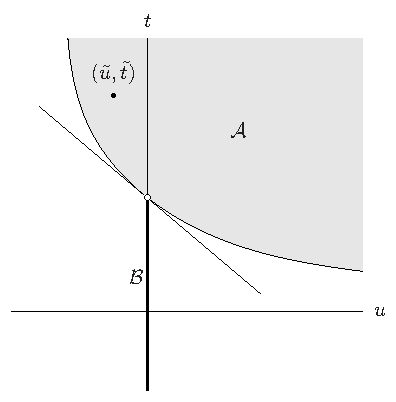
\includegraphics[width=.55\linewidth]{figures/ch05-fig06.pdf}
\caption*{图5.6\quad 满足Slater约束资格的凸问题的强对偶证明示意图。阴影区域为 $\mathcal A$，粗竖线段为 $\mathcal B$，不包含以小空心圆表示的点 $(0,p^\star)$。两个集合凸且不相交，因此可由超平面分离。Slater约束资格保证任意分离超平面都是非竖直的，因为它必须从点 $(\widetilde u,\widetilde t)=(f_1(\widetilde x),f_0(\widetilde x))$ 左侧通过，其中 $\widetilde x$ 严格可行。}
\end{figure}
由于 $f_i(\widetilde x)<0$ 且 $\widetilde\lambda_i\ge0$，可知 $\widetilde\lambda=0$。由 $(\widetilde\lambda,\widetilde\nu,\mu)\ne0$、$\widetilde\lambda=0$ 和 $\mu=0$，可知 $\widetilde\nu\ne0$。于是（5.42）说明，对所有 $x\in D$，$\widetilde\nu^\T(Ax-b)\ge0$。但 $\widetilde x$ 满足 $\widetilde\nu^\T(A\widetilde x-b)=0$，且 $\widetilde x\in\operatorname{int}D$，所以除非 $A^\T\widetilde\nu=0$，否则 $D$ 中必有点满足 $\widetilde\nu^\T(Ax-b)<0$。这当然与假设 $\rank A=p$ 矛盾。

图5.6用只有一个不等式约束的简单问题说明证明背后的几何思想。分离 $\mathcal A$ 和 $\mathcal B$ 的超平面在 $(0,p^\star)$ 处支撑 $\mathcal A$。Slater约束资格用来证明该超平面必非竖直（即法向量可写为 $(\lambda^\star,1)$）。（一个只有一个不等式约束但强对偶失败的简单凸问题，见习题5.21。）

\subsection{多准则解释}
不含等式约束的问题
\begin{equation}
\begin{array}{ll}\text{最小化}&f_0(x)\\
\text{约束为}&f_i(x)\le0,\quad i=1,\ldots,m\end{array}\tag{5.43}
\end{equation}
的拉格朗日对偶，与无约束多准则问题的标量化方法之间存在自然联系。

% Source PDF page 251 (printed p. 237)
这里的多准则问题为
\begin{equation}
\text{最小化（相对于 $\R_+^{m+1}$）}\quad
F(x)=(f_1(x),\ldots,f_m(x),f_0(x))\tag{5.44}
\end{equation}
（见§4.7.4）。标量化时，选择正向量 $\widetilde\lambda$，并最小化标量函数 $\widetilde\lambda^\T F(x)$；任意最小点都保证是Pareto最优的。将 $\widetilde\lambda$ 乘正数不影响最小点，因此不失一般性，可取 $\widetilde\lambda=(\lambda,1)$。于是标量化所最小化的函数是
\[
\widetilde\lambda^\T F(x)=f_0(x)+\sum_{i=1}^m\lambda_i f_i(x),
\]
它恰好是问题（5.43）的拉格朗日函数。

为证明凸多准则问题的每个Pareto最优点，都在某个非负权向量 $\widetilde\lambda$ 下最小化 $\widetilde\lambda^\T F(x)$，我们曾考虑（4.62）定义的集合 $\mathcal A$，
\[
\mathcal A=\{t\in\R^{m+1}\mid\exists x\in D,\ f_i(x)\le t_i,\ i=0,\ldots,m\}.
\]
它与拉格朗日对偶中（5.37）定义的集合 $\mathcal A$ 完全相同。这里同样通过任意Pareto最优点处的支撑超平面来构造所需的权向量。在多准则优化中，权向量各分量表示目标函数之间的相对权重。当把对应于 $f_0$ 的最后一个分量固定为1时，其他权重就表示相对于 $f_0$ 的代价，即相对于目标的代价。

\section{鞍点解释}
本节给出拉格朗日对偶的几种解释。后续内容不会用到本节材料。

\subsection{弱对偶与强对偶的最大—最小刻画}
可以用更对称的形式表示原始和对偶优化问题。为简化讨论，假设没有等式约束；这些结果很容易推广到含等式约束的情况。

首先注意，
\[
\begin{aligned}
\sup_{\lambda\succeq0}L(x,\lambda)
&=\sup_{\lambda\succeq0}\left(f_0(x)+\sum_{i=1}^m\lambda_i f_i(x)\right)\\
&=\begin{cases}
f_0(x)&f_i(x)\le0,\quad i=1,\ldots,m,\\
\infty&\text{其他情形}.
\end{cases}
\end{aligned}
\]

% Source PDF page 252 (printed p. 238)
事实上，若 $x$ 不可行，且某个 $i$ 满足 $f_i(x)>0$，取 $\lambda_j=0$（$j\ne i$），再令 $\lambda_i\to\infty$，就有 $\sup_{\lambda\succeq0}L(x,\lambda)=\infty$。另一方面，若 $f_i(x)\le0$，$i=1,\ldots,m$，则 $\lambda$ 的最优选择是零，因而 $\sup_{\lambda\succeq0}L(x,\lambda)=f_0(x)$。这说明原始问题的最优值可写为
\[
p^\star=\inf_x\sup_{\lambda\succeq0}L(x,\lambda).
\]
由对偶函数定义，还有
\[
d^\star=\sup_{\lambda\succeq0}\inf_xL(x,\lambda).
\]
因此，弱对偶可表示为不等式
\begin{equation}
\sup_{\lambda\succeq0}\inf_xL(x,\lambda)
\le\inf_x\sup_{\lambda\succeq0}L(x,\lambda),\tag{5.45}
\end{equation}
强对偶则表示为等式
\[
\sup_{\lambda\succeq0}\inf_xL(x,\lambda)
=\inf_x\sup_{\lambda\succeq0}L(x,\lambda).
\]
强对偶意味着，关于 $x$ 的最小化和关于 $\lambda\succeq0$ 的最大化可以交换次序，而不改变结果。

事实上，不等式（5.45）不依赖于 $L$ 的任何性质：对任意 $f:\R^n\times\R^m\to\R$（以及任意 $W\subseteq\R^n$、$Z\subseteq\R^m$），有
\begin{equation}
\sup_{z\in Z}\inf_{w\in W}f(w,z)
\le\inf_{w\in W}\sup_{z\in Z}f(w,z).\tag{5.46}
\end{equation}
这一一般不等式称为\emph{最大—最小不等式}。当等号成立，即
\begin{equation}
\sup_{z\in Z}\inf_{w\in W}f(w,z)
=\inf_{w\in W}\sup_{z\in Z}f(w,z),\tag{5.47}
\end{equation}
就称 $f$（以及 $W,Z$）满足\emph{强最大—最小性质}或\emph{鞍点性质}。强最大—最小性质当然只在特殊情形下成立，例如 $f:\R^n\times\R^m\to\R$ 是一个具有强对偶的问题的拉格朗日函数，$W=\R^n$、$Z=\R_+^m$ 时。

\subsection{鞍点解释}
若 $\widetilde w\in W$、$\widetilde z\in Z$ 满足对所有 $w\in W$、$z\in Z$，
\[
f(\widetilde w,z)\le f(\widetilde w,\widetilde z)\le f(w,\widetilde z),
\]
就称 $(\widetilde w,\widetilde z)$ 为 $f$（以及 $W,Z$）的\emph{鞍点}。换言之，$\widetilde w$ 在 $w\in W$ 上最小化 $f(w,\widetilde z)$，$\widetilde z$ 在 $z\in Z$ 上最大化 $f(\widetilde w,z)$：
\[
f(\widetilde w,\widetilde z)=\inf_{w\in W}f(w,\widetilde z),\qquad
f(\widetilde w,\widetilde z)=\sup_{z\in Z}f(\widetilde w,z).
\]

% Source PDF page 253 (printed p. 239)
由此可知强最大—最小性质（5.47）成立，且共同值为 $f(\widetilde w,\widetilde z)$。

回到拉格朗日对偶：若一个强对偶成立的问题中，$x^\star$ 和 $\lambda^\star$ 分别为原始和对偶最优点，它们就构成拉格朗日函数的一个鞍点。反之也成立：若 $(x,\lambda)$ 是拉格朗日函数的鞍点，那么 $x$ 是原始最优点，$\lambda$ 是对偶最优点，且最优对偶间隙为零。

\subsection{博弈解释}
可以用一个连续零和博弈解释最大—最小不等式（5.46）、最大—最小等式（5.47）和鞍点性质。若参与者1选择 $w\in W$，参与者2选择 $z\in Z$，则参与者1向参与者2支付 $f(w,z)$。因此参与者1希望最小化 $f$，参与者2则希望最大化 $f$。（之所以称为连续博弈，是因为选择是向量，而非离散选项。）

假设参与者1先选择，然后参与者2在获知参与者1的选择后再选择。参与者2希望最大化支付 $f(w,z)$，因此将选择 $z\in Z$ 使 $f(w,z)$ 最大。所得支付为 $\sup_{z\in Z}f(w,z)$，它依赖于参与者1的选择 $w$。（这里假设上确界能达到；若不能，最优支付可任意接近 $\sup_{z\in Z}f(w,z)$。）参与者1知道（或假定）参与者2将采取这个策略，因此选择 $w\in W$，使最坏情况下向参与者2的支付尽可能小。于是参与者1选择
\[
\argmin_{w\in W}\sup_{z\in Z}f(w,z),
\]
得到从参与者1向参与者2的支付
\[
\inf_{w\in W}\sup_{z\in Z}f(w,z).
\]

再假设行动次序颠倒：参与者2必须先选择 $z\in Z$，然后参与者1在知道 $z$ 的情况下选择 $w\in W$。类似地，若双方采取最优策略，参与者2应选择 $z\in Z$ 最大化 $\inf_{w\in W}f(w,z)$，从而得到从参与者1向参与者2的支付
\[
\sup_{z\in Z}\inf_{w\in W}f(w,z).
\]

最大—最小不等式（5.46）表达了一个直观事实：后行动对参与者更有利，更准确地说，在作选择前知道对手的选择更有利。换言之，若参与者1必须先选，参与者2得到的支付会更大。当鞍点性质（5.47）成立时，后行动就没有优势。

若 $(\widetilde w,\widetilde z)$ 是 $f$（以及 $W,Z$）的鞍点，便称它为博弈的\emph{解}；称 $\widetilde w$ 为参与者1的\emph{最优选择}或\emph{最优策略}，称 $\widetilde z$ 为参与者2的最优选择或最优策略。

% Source PDF page 254 (printed p. 240)
这时后行动没有优势。

现在考虑支付函数为拉格朗日函数、$W=\R^n$、$Z=\R_+^m$ 的特殊情形。此时参与者1选择原始变量 $x$，参与者2选择对偶变量 $\lambda\succeq0$。根据上面的论证，若参与者2必须先选，她的最优选择就是任意对偶最优的 $\lambda^\star$，由此得到支付 $d^\star$。反之，若参与者1必须先选，他的最优选择是任意原始最优的 $x^\star$，得到支付 $p^\star$。

问题的最优对偶间隙，恰好等于后行动的参与者所获得的优势，也就是在作选择前知道对手选择的优势。若强对偶成立，知道对手的选择对双方都不带来优势。

\subsection{价格或税收解释}
拉格朗日对偶有一个有趣的经济解释。设变量 $x$ 表示企业的运营方式，$f_0(x)$ 表示在 $x$ 下的运营成本，即 $-f_0(x)$ 是运营状态 $x$ 下的利润（例如以美元计）。每个约束 $f_i(x)\le0$ 表示某种限制，例如资源限制（仓储空间、劳动力等）或监管限制（如环保限制）。在遵守限制的同时实现利润最大的运营状态，可通过求解问题
\[
\begin{array}{ll}\text{最小化}&f_0(x)\\
\text{约束为}&f_i(x)\le0,\quad i=1,\ldots,m\end{array}
\]
得到。最优利润为 $-p^\star$。

再设想第二种情形：允许违反限制，但需要支付一笔与违反程度（由 $f_i$ 衡量）成线性关系的额外成本。因此，企业针对第 $i$ 个限制或约束支付 $\lambda_i f_i(x)$。对不紧的约束，也会向企业付款；若 $f_i(x)<0$，则 $\lambda_i f_i(x)$ 表示向企业支付的一笔钱。系数 $\lambda_i$ 可理解为违反 $f_i(x)\le0$ 的价格，单位是每单位违反量（由 $f_i$ 衡量）所需的美元数。企业还能以同一价格出售第 $i$ 个约束的“未用”部分。假设 $\lambda_i\ge0$，即企业要为违反约束付款（若约束不紧，则获得收入）。

例如，原问题第一个约束 $f_1(x)\le0$ 表示仓储空间限制（以平方米计）。在新安排下，企业可以按每平方米 $\lambda_1$ 美元的价格租入额外仓储空间，也可以同样的价格出租未使用空间。

运营状态为 $x$、约束价格为 $\lambda_i$ 时，企业总成本为
$L(x,\lambda)=f_0(x)+\sum_{i=1}^m\lambda_i f_i(x)$。企业显然会选择最小化总成本 $L(x,\lambda)$ 的运营方式，得到成本 $g(\lambda)$。因此，对偶函数表示企业最优成本关于约束价格向量 $\lambda$ 的函数。最优对偶值 $d^\star$ 就是企业在最不利价格组合下的最优成本。

% Source PDF page 255 (printed p. 241)
利用这个解释，弱对偶可表述为：在第二种情形中（允许买卖约束违反量），即使价格最不利，企业的最优成本也不大于原情形（约束不得违反）下的成本。这是明显的：若 $x^\star$ 是第一种情形的最优解，则第二种情形下采用 $x^\star$ 的运营成本会低于 $f_0(x^\star)$，因为不紧的约束还可能带来一些收入。因此，最优对偶间隙就是企业因获准付费违反约束（并因约束不紧而得到款项）所获得的最小可能优势。

现在假设强对偶成立，且对偶最优值能达到。对偶最优的 $\lambda^\star$ 可解释为一组价格：在这组价格下，允许企业付费违反约束（或因约束不紧而收款）并不带来优势。因此，对偶最优的 $\lambda^\star$ 有时称为原问题的一组\emph{影子价格}。

\section{最优性条件}
提醒读者，除非明确说明，我们并不假设问题（5.1）是凸的。

\subsection{次优性证书与停止准则}
若能找到对偶可行的 $(\lambda,\nu)$，就能确定原始问题最优值的下界：$p^\star\ge g(\lambda,\nu)$。因此，对偶可行点 $(\lambda,\nu)$ 提供 $p^\star\ge g(\lambda,\nu)$ 的一个证明或\emph{证书}。强对偶意味着存在任意精确的证书。

不必知道 $p^\star$ 的精确值，对偶可行点就能为给定可行点的次优程度提供界。事实上，若 $x$ 原始可行、$(\lambda,\nu)$ 对偶可行，则
\[
f_0(x)-p^\star\le f_0(x)-g(\lambda,\nu).
\]
这特别说明，$x$ 是 $\epsilon$-次优的，其中 $\epsilon=f_0(x)-g(\lambda,\nu)$。（同时也说明 $(\lambda,\nu)$ 是对偶问题的 $\epsilon$-次优点。）

把原始和对偶目标之间的差
\[
f_0(x)-g(\lambda,\nu)
\]
称为原始可行点 $x$ 与对偶可行点 $(\lambda,\nu)$ 对应的\emph{对偶间隙}。原始—对偶可行点对 $x,(\lambda,\nu)$ 将原始（及对偶）问题的最优值定位在区间内：
\[
p^\star\in[g(\lambda,\nu),f_0(x)],\qquad
d^\star\in[g(\lambda,\nu),f_0(x)],
\]
区间宽度就是对偶间隙。

若原始—对偶可行点对 $x,(\lambda,\nu)$ 的对偶间隙为零，即 $f_0(x)=g(\lambda,\nu)$，则 $x$ 是原始最优点，$(\lambda,\nu)$ 是对偶最优点。可以把 $(\lambda,\nu)$ 看作证明 $x$ 最优的证书。

% Source PDF page 256 (printed p. 242)
类似地，也可把 $x$ 看作证明 $(\lambda,\nu)$ 对偶最优的证书。

在优化算法中，这些观察可用于给出非启发式停止准则。假设算法产生原始可行序列 $x^{(k)}$ 和对偶可行序列 $(\lambda^{(k)},\nu^{(k)})$，$k=1,2,\ldots$，给定所需绝对精度 $\epsilon_{\mathrm{abs}}>0$。那么停止准则（即终止算法的条件）
\[
f_0(x^{(k)})-g(\lambda^{(k)},\nu^{(k)})\le\epsilon_{\mathrm{abs}}
\]
保证算法终止时，$x^{(k)}$ 是 $\epsilon_{\mathrm{abs}}$-次优的。事实上，$(\lambda^{(k)},\nu^{(k)})$ 就是证明这一点的证书。（当然，要使此方法对任意小容差 $\epsilon_{\mathrm{abs}}$ 有效，必须有强对偶。）

类似条件可以保证给定相对精度 $\epsilon_{\mathrm{rel}}>0$。若
\[
g(\lambda^{(k)},\nu^{(k)})>0,\qquad
\frac{f_0(x^{(k)})-g(\lambda^{(k)},\nu^{(k)})}
{g(\lambda^{(k)},\nu^{(k)})}\le\epsilon_{\mathrm{rel}},
\]
或
\[
f_0(x^{(k)})<0,\qquad
\frac{f_0(x^{(k)})-g(\lambda^{(k)},\nu^{(k)})}
{-f_0(x^{(k)})}\le\epsilon_{\mathrm{rel}},
\]
则 $p^\star\ne0$，且相对误差
\[
\frac{f_0(x^{(k)})-p^\star}{|p^\star|}
\]
保证不大于 $\epsilon_{\mathrm{rel}}$。

\subsection{互补松弛}
假设原始和对偶最优值都能达到且相等（特别地，强对偶成立）。设 $x^\star$ 是原始最优点，$(\lambda^\star,\nu^\star)$ 是对偶最优点。这意味着
\[
\begin{aligned}
f_0(x^\star)&=g(\lambda^\star,\nu^\star)\\
&=\inf_x\left(f_0(x)+\sum_{i=1}^m\lambda_i^\star f_i(x)
+\sum_{i=1}^p\nu_i^\star h_i(x)\right)\\
&\le f_0(x^\star)+\sum_{i=1}^m\lambda_i^\star f_i(x^\star)
+\sum_{i=1}^p\nu_i^\star h_i(x^\star)\\
&\le f_0(x^\star).
\end{aligned}
\]
第一行表示最优对偶间隙为零，第二行是对偶函数的定义。第三行源于拉格朗日函数关于 $x$ 的下确界不大于它在 $x=x^\star$ 的取值。最后一个不等式源于 $\lambda_i^\star\ge0$、$f_i(x^\star)\le0$，$i=1,\ldots,m$，及 $h_i(x^\star)=0$，$i=1,\ldots,p$。因此，不等式链中的两个不等式都必须取等号。

% Source PDF page 257 (printed p. 243)
由此能得出几个有趣结论。例如，第三行不等式取等号说明 $x^\star$ 关于 $x$ 最小化 $L(x,\lambda^\star,\nu^\star)$。（拉格朗日函数 $L(x,\lambda^\star,\nu^\star)$ 还可能有其他最小点；$x^\star$ 只是其中之一。）

另一个重要结论是
\[
\sum_{i=1}^m\lambda_i^\star f_i(x^\star)=0.
\]
由于和式中每项都非正，可知
\begin{equation}
\lambda_i^\star f_i(x^\star)=0,\quad i=1,\ldots,m.\tag{5.48}
\end{equation}
这一条件称为\emph{互补松弛}；当强对偶成立时，它对任意原始最优 $x^\star$ 和任意对偶最优 $(\lambda^\star,\nu^\star)$ 都成立。互补松弛可写为
\[
\lambda_i^\star>0\ \Longrightarrow\ f_i(x^\star)=0,
\]
或等价地，
\[
f_i(x^\star)<0\ \Longrightarrow\ \lambda_i^\star=0.
\]
粗略地说，除非第 $i$ 个约束在最优点处是活跃的，否则第 $i$ 个最优拉格朗日乘子为零。

\subsection{KKT最优性条件}
现在假设 $f_0,\ldots,f_m,h_1,\ldots,h_p$ 可微（因此其定义域为开集），但仍未对凸性作假设。

\subsubsection*{非凸问题的KKT条件}
同上，设 $x^\star$ 和 $(\lambda^\star,\nu^\star)$ 是任意一对对偶间隙为零的原始、对偶最优点。由于 $x^\star$ 关于 $x$ 最小化 $L(x,\lambda^\star,\nu^\star)$，其梯度必在 $x^\star$ 处为零，即
\[
\nabla f_0(x^\star)+\sum_{i=1}^m\lambda_i^\star\nabla f_i(x^\star)
+\sum_{i=1}^p\nu_i^\star\nabla h_i(x^\star)=0.
\]
因此有
\begin{equation}
\begin{gathered}
f_i(x^\star)\le0,\quad i=1,\ldots,m,\\
h_i(x^\star)=0,\quad i=1,\ldots,p,\\
\lambda_i^\star\ge0,\quad i=1,\ldots,m,\\
\lambda_i^\star f_i(x^\star)=0,\quad i=1,\ldots,m,\\
\nabla f_0(x^\star)+\sum_{i=1}^m\lambda_i^\star\nabla f_i(x^\star)
+\sum_{i=1}^p\nu_i^\star\nabla h_i(x^\star)=0,
\end{gathered}\tag{5.49}
\end{equation}
这些条件称为\emph{Karush--Kuhn--Tucker（KKT）条件}。

综上，对于目标函数和约束函数都可微、且强对偶成立的任意优化问题，任意一对原始和对偶最优点都必须满足KKT条件（5.49）。

% Source PDF page 258 (printed p. 244)
\subsubsection*{凸问题的KKT条件}
当原始问题凸时，KKT条件也是原始和对偶最优的充分条件。换言之，若 $f_i$ 凸、$h_i$ 仿射，且 $\widetilde x,\widetilde\lambda,\widetilde\nu$ 满足KKT条件
\[
\begin{gathered}
f_i(\widetilde x)\le0,\quad i=1,\ldots,m,\\
h_i(\widetilde x)=0,\quad i=1,\ldots,p,\\
\widetilde\lambda_i\ge0,\quad i=1,\ldots,m,\\
\widetilde\lambda_i f_i(\widetilde x)=0,\quad i=1,\ldots,m,\\
\nabla f_0(\widetilde x)+\sum_{i=1}^m\widetilde\lambda_i\nabla f_i(\widetilde x)
+\sum_{i=1}^p\widetilde\nu_i\nabla h_i(\widetilde x)=0,
\end{gathered}
\]
则 $\widetilde x$、$(\widetilde\lambda,\widetilde\nu)$ 分别是原始和对偶最优点，且对偶间隙为零。

为说明这一点，注意前两个条件表示 $\widetilde x$ 原始可行。由于 $\widetilde\lambda_i\ge0$，$L(x,\widetilde\lambda,\widetilde\nu)$ 关于 $x$ 凸；最后一个KKT条件表示它关于 $x$ 的梯度在 $x=\widetilde x$ 处为零，因此 $\widetilde x$ 关于 $x$ 最小化 $L(x,\widetilde\lambda,\widetilde\nu)$。由此得到
\[
\begin{aligned}
g(\widetilde\lambda,\widetilde\nu)&=L(\widetilde x,\widetilde\lambda,\widetilde\nu)\\
&=f_0(\widetilde x)+\sum_{i=1}^m\widetilde\lambda_i f_i(\widetilde x)
+\sum_{i=1}^p\widetilde\nu_i h_i(\widetilde x)\\
&=f_0(\widetilde x),
\end{aligned}
\]
最后一步利用了 $h_i(\widetilde x)=0$ 和 $\widetilde\lambda_i f_i(\widetilde x)=0$。这说明 $\widetilde x$ 和 $(\widetilde\lambda,\widetilde\nu)$ 的对偶间隙为零，因此分别原始最优和对偶最优。综上，对于任意目标和约束函数均可微的凸优化问题，满足KKT条件的点就是原始和对偶最优点，且对偶间隙为零。

若目标和约束函数均可微的凸优化问题满足Slater条件，那么KKT条件给出最优性的充要条件：Slater条件蕴含最优对偶间隙为零且对偶最优值能达到，所以 $x$ 最优，当且仅当存在 $(\lambda,\nu)$，与 $x$ 一起满足KKT条件。

KKT条件在优化中起重要作用。少数特殊情形下，可以解析地求解KKT条件（从而求解优化问题）。更一般地，许多凸优化算法本来就是，或可以解释为，求解KKT条件的方法。

\begin{origexample}{5.1}
\emph{等式约束凸二次最小化。}考虑问题
\begin{equation}
\begin{array}{ll}\text{最小化}&(1/2)x^\T Px+q^\T x+r\\
\text{约束为}&Ax=b,\end{array}\tag{5.50}
\end{equation}
其中 $P\in\mathbf S_+^n$。该问题的KKT条件为
\[
Ax^\star=b,\qquad Px^\star+q+A^\T\nu^\star=0,
\]
可写为
\[
\begin{bmatrix}P&A^\T\\A&0\end{bmatrix}
\begin{bmatrix}x^\star\\\nu^\star\end{bmatrix}
=\begin{bmatrix}-q\\b\end{bmatrix}.
\]

% Source PDF page 259 (printed p. 245)
求解这组含 $m+n$ 个方程、$m+n$ 个变量 $x^\star,\nu^\star$ 的方程组，即可得到（5.50）的最优原始和对偶变量。
\end{origexample}

\begin{origexample}{5.2}
\emph{注水。}考虑凸优化问题
\[
\begin{array}{ll}\text{最小化}&-\sum_{i=1}^n\log(\alpha_i+x_i)\\
\text{约束为}&x\succeq0,\quad\one^\T x=1,\end{array}
\]
其中 $\alpha_i>0$。这一问题出现在信息论中，用于向 $n$ 个通信信道分配功率。变量 $x_i$ 是分配给第 $i$ 个信道的发射功率，$\log(\alpha_i+x_i)$ 给出信道容量或通信速率，因此问题是将总量为1的功率分配给各信道，使总通信速率最大。

对不等式约束 $x^\star\succeq0$ 引入拉格朗日乘子 $\lambda^\star\in\R^n$，对等式约束 $\one^\T x=1$ 引入乘子 $\nu^\star\in\R$，得到KKT条件
\[
\begin{gathered}
x^\star\succeq0,\quad\one^\T x^\star=1,\quad\lambda^\star\succeq0,\quad
\lambda_i^\star x_i^\star=0,\quad i=1,\ldots,n,\\
-1/(\alpha_i+x_i^\star)-\lambda_i^\star+\nu^\star=0,\quad i=1,\ldots,n.
\end{gathered}
\]
可以直接求解这些方程，得到 $x^\star,\lambda^\star,\nu^\star$。首先注意，$\lambda^\star$ 在最后一个方程中起松弛变量的作用，可将其消去，得到
\[
\begin{gathered}
x^\star\succeq0,\quad \one^\T x^\star=1,\quad
x_i^\star\bigl(\nu^\star-1/(\alpha_i+x_i^\star)\bigr)=0,\quad i=1,\ldots,n,\\
\nu^\star\ge1/(\alpha_i+x_i^\star),\quad i=1,\ldots,n.
\end{gathered}
\]
若 $\nu^\star<1/\alpha_i$，最后一个条件只有在 $x_i^\star>0$ 时才可能成立；再由第三个条件，得到 $\nu^\star=1/(\alpha_i+x_i^\star)$。解出 $x_i^\star$，可知当 $\nu^\star<1/\alpha_i$ 时，$x_i^\star=1/\nu^\star-\alpha_i$。若 $\nu^\star\ge1/\alpha_i$，则不可能有 $x_i^\star>0$，否则将有 $\nu^\star\ge1/\alpha_i>1/(\alpha_i+x_i^\star)$，违反互补松弛。因此，当 $\nu^\star\ge1/\alpha_i$ 时，$x_i^\star=0$。所以
\[
x_i^\star=\begin{cases}
1/\nu^\star-\alpha_i&\nu^\star<1/\alpha_i,\\
0&\nu^\star\ge1/\alpha_i,
\end{cases}
\]
更简洁地，$x_i^\star=\max\{0,1/\nu^\star-\alpha_i\}$。代入 $\one^\T x^\star=1$，得到
\[
\sum_{i=1}^n\max\{0,1/\nu^\star-\alpha_i\}=1.
\]
左端是关于 $1/\nu^\star$ 的分段线性递增函数，折点为 $\alpha_i$，因此方程有容易求出的唯一解。

这种求解方法称为\emph{注水}，原因如下。将 $\alpha_i$ 看作第 $i$ 块地面的高度，然后向区域注水，水位为 $1/\nu$，如图5.7所示。总用水量为 $\sum_{i=1}^n\max\{0,1/\nu^\star-\alpha_i\}$。逐渐提高水位，直到总用水量恰为1。此时第 $i$ 块地面上方的水深就是最优值 $x_i^\star$。
\end{origexample}

% Source PDF page 260 (printed p. 246)
\begin{figure}[htbp]\centering
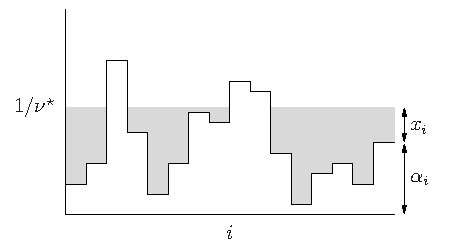
\includegraphics[width=.65\linewidth]{figures/ch05-fig07.pdf}
\caption*{图5.7\quad 注水算法示意图。各块地面的高度为 $\alpha_i$。将区域注水到水位 $1/\nu^\star$，总用水量为1。各块地面上方的水深（阴影部分）就是 $x_i^\star$ 的最优值。}
\end{figure}
\begin{figure}[htbp]\centering
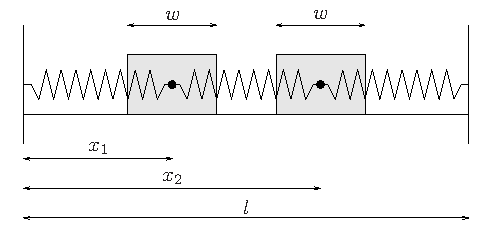
\includegraphics[width=.65\linewidth]{figures/ch05-fig08.pdf}
\caption*{图5.8\quad 两个物块由弹簧相互连接，并与左右墙壁连接。物块宽度为 $w>0$，不能相互穿透，也不能穿过墙壁。}
\end{figure}

\subsection{KKT条件的力学解释}
KKT条件在力学中有一个很好的解释（这事实上也是Lagrange的主要动机之一）。用一个简单例子来说明。图5.8中的系统由两个物块组成，三个弹簧将它们相互连接，并连接到左右墙壁。物块位置由 $x\in\R^2$ 给出，$x_1$ 是左侧物块（中心）的位移，$x_2$ 是右侧物块的位移。左墙位置为0，右墙位置为 $l$。

弹簧势能是物块位置的函数：
\[
f_0(x_1,x_2)=\frac12k_1x_1^2+\frac12k_2(x_2-x_1)^2+\frac12k_3(l-x_2)^2,
\]
其中 $k_i>0$ 为三个弹簧的刚度系数。平衡位置 $x^\star$ 是在以下不等式约束下使势能最小的位置：
\begin{equation}
w/2-x_1\le0,\qquad w+x_1-x_2\le0,\qquad w/2-l+x_2\le0.\tag{5.51}
\end{equation}

% Source PDF page 261 (printed p. 247)
\begin{figure}[htbp]\centering
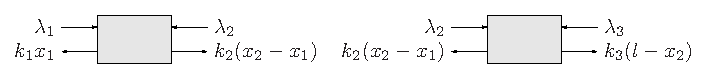
\includegraphics[width=.85\linewidth]{figures/ch05-fig09.pdf}
\caption*{图5.9\quad 物块—弹簧系统的受力分析。弹簧力和接触力作用在每个物块上的合力必须为零。上方所示拉格朗日乘子是墙壁与物块之间的接触力，下方表示弹簧力。}
\end{figure}
这些约束称为\emph{运动学约束}，表达物块宽度为 $w>0$、不能相互穿透或穿过墙壁这一事实。因此，平衡位置由下列二次规划的解给出：
\begin{equation}
\begin{array}{ll}
\text{最小化}&(1/2)\bigl(k_1x_1^2+k_2(x_2-x_1)^2+k_3(l-x_2)^2\bigr)\\
\text{约束为}&w/2-x_1\le0\\
&w+x_1-x_2\le0\\
&w/2-l+x_2\le0.
\end{array}\tag{5.52}
\end{equation}
取 $\lambda_1,\lambda_2,\lambda_3$ 为拉格朗日乘子，该问题的KKT条件由运动学约束（5.51）、非负约束 $\lambda_i\ge0$、互补松弛条件
\begin{equation}
\begin{gathered}
\lambda_1(w/2-x_1)=0,\quad
\lambda_2(w-x_2+x_1)=0,\\
\lambda_3(w/2-l+x_2)=0,
\end{gathered}\tag{5.53}
\end{equation}
以及零梯度条件
\begin{equation}
\begin{bmatrix}k_1x_1-k_2(x_2-x_1)\\k_2(x_2-x_1)-k_3(l-x_2)\end{bmatrix}
+\lambda_1\begin{bmatrix}-1\\0\end{bmatrix}
+\lambda_2\begin{bmatrix}1\\-1\end{bmatrix}
+\lambda_3\begin{bmatrix}0\\1\end{bmatrix}=0\tag{5.54}
\end{equation}
组成。

如果把拉格朗日乘子解释为墙壁与物块之间的接触力，方程（5.54）就可理解为两个物块的力平衡方程，如图5.9所示。第一个方程表示第一个物块上的合力为零：$-k_1x_1$ 是左弹簧对左物块的作用力，$k_2(x_2-x_1)$ 是中间弹簧的作用力，$\lambda_1$ 是左墙的作用力，$-\lambda_2$ 是右物块的作用力。接触力必须指向离开接触面的方向（由 $\lambda_1\ge0$、$-\lambda_2\le0$ 表达），并且只有发生接触时才非零（由前两个互补松弛条件（5.53）表达）。类似地，（5.54）的第二个方程是第二个物块的力平衡方程；（5.53）的最后一个条件表示，除非右物块碰到墙壁，否则 $\lambda_3$ 为零。

这个例子中，势能和运动学约束函数均凸，而且只要 $2w\le l$，即两墙之间有足够空间容纳两个物块，就满足Slater约束资格的放宽形式。因此可知，由（5.52）给出的平衡能量表述，与KKT条件给出的力平衡表述产生相同结果。

% Source PDF page 262 (printed p. 248)
\subsection{通过对偶求解原始问题}
在§5.5.3开头已提到，若强对偶成立且对偶最优解 $(\lambda^\star,\nu^\star)$ 存在，那么任意原始最优点也是 $L(x,\lambda^\star,\nu^\star)$ 的最小点。有时可利用这一事实，从对偶最优解计算原始最优解。

更准确地说，假设有强对偶且已知最优的 $(\lambda^\star,\nu^\star)$。再假设 $L(x,\lambda^\star,\nu^\star)$ 的最小点，即问题
\begin{equation}
\text{最小化}\quad f_0(x)+\sum_{i=1}^m\lambda_i^\star f_i(x)
+\sum_{i=1}^p\nu_i^\star h_i(x)\tag{5.55}
\end{equation}
的解是唯一的。（对于凸问题，例如当 $L(x,\lambda^\star,\nu^\star)$ 关于 $x$ 严格凸时，就会如此。）若（5.55）的解原始可行，则它必定原始最优；若它原始不可行，则原始最优点不可能存在，即可知原始最优值不能达到。当对偶问题比原始问题容易求解时，例如对偶可以解析求解，或具有可利用的特殊结构时，这一观察很有意义。

\begin{origexample}{5.3}
\emph{熵最大化。}考虑熵最大化问题
\[
\begin{array}{ll}\text{最小化}&f_0(x)=\sum_{i=1}^n x_i\log x_i\\
\text{约束为}&Ax\preceq b\\&\one^\T x=1,\end{array}
\]
定义域为 $\R_{++}^n$。它的对偶为
\[
\begin{array}{ll}\text{最大化}&-b^\T\lambda-\nu-e^{-\nu-1}\sum_{i=1}^n e^{-a_i^\T\lambda}\\
\text{约束为}&\lambda\succeq0,\end{array}
\]
其中 $a_i$ 是 $A$ 的各列（见第222、228页）。假设较弱的Slater条件成立，即存在 $x\succ0$ 满足 $Ax\preceq b$、$\one^\T x=1$。因此强对偶成立，且最优解 $(\lambda^\star,\nu^\star)$ 存在。

设已求出对偶问题的解。在 $(\lambda^\star,\nu^\star)$ 处的拉格朗日函数为
\[
L(x,\lambda^\star,\nu^\star)=\sum_{i=1}^n x_i\log x_i
+(\lambda^\star)^\T(Ax-b)+\nu^\star(\one^\T x-1).
\]
它在 $D$ 上严格凸且有下界，所以有唯一解 $x^\star$，由下式给出：
\[
x_i^\star=1/\exp(a_i^\T\lambda^\star+\nu^\star+1),\quad i=1,\ldots,n.
\]
若 $x^\star$ 原始可行，则必为原始问题（5.13）的最优解；若 $x^\star$ 原始不可行，则可知原始最优值不能达到。
\end{origexample}

\begin{origexample}{5.4}
\emph{等式约束下可分函数的最小化。}考虑问题
\[
\begin{array}{ll}\text{最小化}&f_0(x)=\sum_{i=1}^n f_i(x_i)\\
\text{约束为}&a^\T x=b,\end{array}
\]

% Source PDF page 263 (printed p. 249)
其中 $a\in\R^n$、$b\in\R$，$f_i:\R\to\R$ 可微且严格凸。目标函数称为\emph{可分的}，因为它是各个变量 $x_1,\ldots,x_n$ 的函数之和。假设 $f_0$ 的定义域与约束集相交，即存在 $x_0\in\dom f_0$ 使 $a^\T x_0=b$。这意味着问题有唯一最优点 $x^\star$。

拉格朗日函数为
\[
L(x,\nu)=\sum_{i=1}^n f_i(x_i)+\nu(a^\T x-b)
=-b\nu+\sum_{i=1}^n(f_i(x_i)+\nu a_i x_i),
\]
同样是可分的，故对偶函数为
\[
\begin{aligned}
g(\nu)&=-b\nu+\inf_x\left(\sum_{i=1}^n(f_i(x_i)+\nu a_i x_i)\right)\\
&=-b\nu+\sum_{i=1}^n\inf_{x_i}(f_i(x_i)+\nu a_i x_i)\\
&=-b\nu-\sum_{i=1}^n f_i^*(-\nu a_i).
\end{aligned}
\]
因此对偶问题为
\[
\text{最大化}\quad -b\nu-\sum_{i=1}^n f_i^*(-\nu a_i),
\]
其（标量）变量为 $\nu\in\R$。

现在设已找到最优对偶变量 $\nu^\star$。（具有一个标量变量的凸问题有几种简单求法，例如二分法。）由于各 $f_i$ 严格凸，$L(x,\nu^\star)$ 关于 $x$ 严格凸，所以有唯一最小点 $\widetilde x$。而且已知 $x^\star$ 也最小化 $L(x,\nu^\star)$，故必有 $\widetilde x=x^\star$。可由 $\nabla_xL(x,\nu^\star)=0$ 恢复 $x^\star$，即求解方程 $f_i'(x_i^\star)=-\nu^\star a_i$。
\end{origexample}

\section{扰动与灵敏度分析}
当强对偶成立时，最优对偶变量对最优值关于约束扰动的灵敏度提供非常有用的信息。

\subsection{扰动问题}
考虑原优化问题（5.1）的如下扰动版本：
\begin{equation}
\begin{array}{ll}\text{最小化}&f_0(x)\\
\text{约束为}&f_i(x)\le u_i,\quad i=1,\ldots,m\\
&h_i(x)=v_i,\quad i=1,\ldots,p,\end{array}\tag{5.56}
\end{equation}

% Source PDF page 264 (printed p. 250)
变量为 $x\in\R^n$。当 $u=0,v=0$ 时，它就是原问题（5.1）。$u_i$ 为正表示放宽第 $i$ 个不等式约束，为负则表示收紧约束。因此，扰动问题（5.56）由原问题（5.1）通过将每个不等式约束收紧或放宽 $u_i$、将等式约束右端改变 $v_i$ 得到。

定义 $p^\star(u,v)$ 为扰动问题（5.56）的最优值：
\[
\begin{split}
p^\star(u,v)=\inf\{f_0(x)\mid{}&\exists x\in D,\ f_i(x)\le u_i,\ i=1,\ldots,m,\\
&h_i(x)=v_i,\ i=1,\ldots,p\}.
\end{split}
\]
可能出现 $p^\star(u,v)=\infty$，对应于使问题不可行的约束扰动。注意 $p^\star(0,0)=p^\star$，即未扰动问题（5.1）的最优值。（希望这种略微混用记号的做法不会造成混淆。）粗略地说，函数 $p^\star:\R^m\times\R^p\to\R$ 给出最优值关于约束右端扰动的函数关系。

当原问题凸时，$p^\star$ 是关于 $u,v$ 的凸函数；事实上，其上图恰好是（5.37）定义的集合 $\mathcal A$ 的闭包（见习题5.32）。

\subsection{一个全局不等式}
现在假设强对偶成立，且对偶最优值能达到。（若原问题凸且满足Slater条件，就属于这种情况。）设 $(\lambda^\star,\nu^\star)$ 是未扰动问题的对偶（5.16）的最优解。那么，对于所有 $u,v$，都有
\begin{equation}
p^\star(u,v)\ge p^\star(0,0)-(\lambda^\star)^\T u-(\nu^\star)^\T v.\tag{5.57}
\end{equation}
为证明该不等式，设 $x$ 是扰动问题任意可行点，即 $f_i(x)\le u_i$，$i=1,\ldots,m$，$h_i(x)=v_i$，$i=1,\ldots,p$。由强对偶，
\[
\begin{aligned}
p^\star(0,0)=g(\lambda^\star,\nu^\star)
&\le f_0(x)+\sum_{i=1}^m\lambda_i^\star f_i(x)
+\sum_{i=1}^p\nu_i^\star h_i(x)\\
&\le f_0(x)+(\lambda^\star)^\T u+(\nu^\star)^\T v.
\end{aligned}
\]
第一个不等式由 $g(\lambda^\star,\nu^\star)$ 定义得到；第二个利用 $\lambda^\star\succeq0$。因此，对于扰动问题任意可行点 $x$，
\[
f_0(x)\ge p^\star(0,0)-(\lambda^\star)^\T u-(\nu^\star)^\T v,
\]
从而得到（5.57）。

\subsubsection*{灵敏度解释}
强对偶成立时，可直接由（5.57）得到最优拉格朗日变量的多种灵敏度解释。部分结论如下：

% Source PDF page 265 (printed p. 251)
\begin{figure}[htbp]\centering
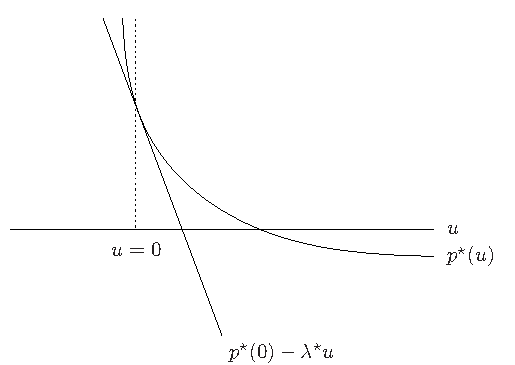
\includegraphics[width=.65\linewidth]{figures/ch05-fig10.pdf}
\caption*{图5.10\quad 含单个约束 $f_1(x)\le u$ 的凸问题的最优值 $p^\star(u)$ 关于 $u$ 的函数。$u=0$ 时为原未扰动问题；$u<0$ 时约束收紧；$u>0$ 时约束放宽。仿射函数 $p^\star(0)-\lambda^\star u$ 是 $p^\star$ 的下界。}
\end{figure}
\begin{itemize}
\item 若 $\lambda_i^\star$ 很大，并收紧第 $i$ 个约束（即取 $u_i<0$），那么最优值 $p^\star(u,v)$ 保证大幅增加。
\item 若 $\nu_i^\star$ 是很大的正数且取 $v_i<0$，或 $\nu_i^\star$ 是绝对值很大的负数且取 $v_i>0$，那么最优值 $p^\star(u,v)$ 保证大幅增加。
\item 若 $\lambda_i^\star$ 很小，并放宽第 $i$ 个约束（$u_i>0$），那么最优值 $p^\star(u,v)$ 不会下降太多。
\item 若 $\nu_i^\star$ 是很小的正数且 $v_i>0$，或 $\nu_i^\star$ 是绝对值很小的负数且 $v_i<0$，那么最优值 $p^\star(u,v)$ 不会下降太多。
\end{itemize}
不等式（5.57）和上述结论给出扰动后最优值的下界，却不提供上界。因此，关于收紧和放宽约束，这些结果并不对称。例如，设 $\lambda_i^\star$ 很大，并稍微放宽第 $i$ 个约束（即取很小的正 $u_i$），这时（5.57）并无用处；例如，它并不意味着最优值会显著下降。

图5.10用一个仅含一个不等式约束的凸问题说明（5.57）。不等式表示，仿射函数 $p^\star(0)-\lambda^\star u$ 是凸函数 $p^\star$ 的下界。

\subsection{局部灵敏度分析}
现在设 $p^\star(u,v)$ 在 $u=0,v=0$ 处可微。那么，只要强对偶成立，最优对偶变量 $\lambda^\star,\nu^\star$ 就与该点处 $p^\star$ 的梯度相关：

% Source PDF page 266 (printed p. 252)
\begin{equation}
\lambda_i^\star=-\frac{\partial p^\star(0,0)}{\partial u_i},
\qquad
\nu_i^\star=-\frac{\partial p^\star(0,0)}{\partial v_i}.\tag{5.58}
\end{equation}
图5.10的例子说明了这一性质：$-\lambda^\star$ 是 $p^\star$ 在 $u=0$ 附近的斜率。

因此，若 $p^\star(u,v)$ 在 $u=0,v=0$ 处可微且强对偶成立，最优拉格朗日乘子恰好给出最优值关于约束扰动的局部灵敏度。与不可微情形不同，这一解释是对称的：将第 $i$ 个不等式约束稍微收紧（取很小的负 $u_i$），使 $p^\star$ 大约增加 $-\lambda_i^\star u_i$；稍微放宽第 $i$ 个约束（取很小的正 $u_i$），使 $p^\star$ 大约下降 $\lambda_i^\star u_i$。

为证明（5.58），设 $p^\star(u,v)$ 可微且强对偶成立。对扰动 $u=te_i,v=0$，其中 $e_i$ 为第 $i$ 个单位向量，有
\[
\lim_{t\to0}\frac{p^\star(te_i,0)-p^\star}{t}
=\frac{\partial p^\star(0,0)}{\partial u_i}.
\]
由（5.57），当 $t>0$ 时，
\[
\frac{p^\star(te_i,0)-p^\star}{t}\ge-\lambda_i^\star,
\]
而 $t<0$ 时不等式方向相反。取 $t>0$ 且 $t\to0$，得到
\[
\frac{\partial p^\star(0,0)}{\partial u_i}\ge-\lambda_i^\star.
\]
从 $t<0$ 一侧取极限，则得到反方向不等式，因此
\[
\frac{\partial p^\star(0,0)}{\partial u_i}=-\lambda_i^\star.
\]
用同样方法可得
\[
\frac{\partial p^\star(0,0)}{\partial v_i}=-\nu_i^\star.
\]

局部灵敏度结果（5.58）定量衡量一个约束在最优点 $x^\star$ 处的活跃程度。若 $f_i(x^\star)<0$，约束不活跃，可将它稍微收紧或放宽，而不影响最优值。由互补松弛，相应最优拉格朗日乘子必为零。再设 $f_i(x^\star)=0$，即第 $i$ 个约束在最优点处活跃。第 $i$ 个最优拉格朗日乘子给出活跃程度：若 $\lambda_i^\star$ 小，表示稍微放宽或收紧约束对最优值影响不大；若 $\lambda_i^\star$ 大，表示稍微放宽或收紧约束会对最优值产生很大影响。

% Source PDF page 267 (printed p. 253)
\subsubsection*{影子价格解释}
还可以用经济学对结果（5.58）作一个简单的几何解释。为简便，考虑不含等式约束、满足Slater条件的凸问题。变量 $x\in\R^m$ 决定企业的运营方式，目标 $f_0$ 为成本，即 $-f_0$ 为利润。每个约束 $f_i(x)\le0$ 代表对某种资源的限制，例如劳动力、钢材或仓储空间。扰动最优成本函数的相反数 $-p^\star(u)$，告诉我们企业得到更多或更少各类资源时，利润会增加或减少多少。如果它在 $u=0$ 附近可微，则
\[
\lambda_i^\star=-\frac{\partial p^\star(0)}{\partial u_i}.
\]
换言之，$\lambda_i^\star$ 近似表示资源 $i$ 的可用量略微增加时，企业能多获得多少利润。

因此，若允许企业买卖资源 $i$，$\lambda_i^\star$ 就是它的自然价格或均衡价格。例如，若企业可以买卖资源 $i$，价格低于 $\lambda_i^\star$，企业当然会买入一些资源，借此改变运营方式，所增加的利润会超过购买资源的成本。反之，若价格高于 $\lambda_i^\star$，企业会卖出部分已分配资源，并获得净收益，因为出售资源的收入高于资源可用量下降造成的利润损失。

\section{例子}
本节通过例子说明，对问题作简单的等价改写，可能得到非常不同的对偶问题。考虑以下改写方式：
\begin{itemize}
\item 引入新变量及相应等式约束。
\item 用原目标的递增函数替代目标。
\item 使显式约束隐含化，即将它们并入目标函数的定义域。
\end{itemize}

\subsection{引入新变量和等式约束}
考虑无约束问题
\begin{equation}
\text{最小化}\quad f_0(Ax+b).\tag{5.59}
\end{equation}
它的拉格朗日对偶函数为常数 $p^\star$。因此，虽然强对偶成立，即 $p^\star=d^\star$，但拉格朗日对偶既无用，也不令人感兴趣。

% Source PDF page 268 (printed p. 254)
现在把（5.59）改写为
\begin{equation}
\begin{array}{ll}\text{最小化}&f_0(y)\\
\text{约束为}&Ax+b=y.\end{array}\tag{5.60}
\end{equation}
这里引入新变量 $y$ 和新等式约束 $Ax+b=y$。问题（5.59）与（5.60）显然等价。

改写后问题的拉格朗日函数为
\[
L(x,y,\nu)=f_0(y)+\nu^\T(Ax+b-y).
\]
对 $x,y$ 最小化 $L$，即可求对偶函数。先对 $x$ 最小化，得到：除非 $A^\T\nu=0$，否则 $g(\nu)=-\infty$；当等式成立时，剩下
\[
g(\nu)=b^\T\nu+\inf_y(f_0(y)-\nu^\T y)=b^\T\nu-f_0^*(\nu),
\]
其中 $f_0^*$ 是 $f_0$ 的共轭。因此（5.60）的对偶可写为
\begin{equation}
\begin{array}{ll}\text{最大化}&b^\T\nu-f_0^*(\nu)\\
\text{约束为}&A^\T\nu=0.\end{array}\tag{5.61}
\end{equation}
所以，改写后问题（5.60）的对偶比原问题（5.59）的对偶有用得多。

\begin{origexample}{5.5}
\emph{无约束几何规划。}考虑无约束几何规划
\[
\text{最小化}\quad\log\left(\sum_{i=1}^m\exp(a_i^\T x+b_i)\right).
\]
首先引入新变量和等式约束，将其改写为
\[
\begin{array}{ll}\text{最小化}&f_0(y)=\log\left(\sum_{i=1}^m\exp y_i\right)\\
\text{约束为}&Ax+b=y,\end{array}
\]
其中 $a_i^\T$ 为 $A$ 的各行。指数和的对数函数的共轭为
\[
f_0^*(\nu)=\begin{cases}
\sum_{i=1}^m\nu_i\log\nu_i&\nu\succeq0,\ \one^\T\nu=1,\\
\infty&\text{其他情形}
\end{cases}
\]
（第93页例3.25），所以改写后问题的对偶可写为
\begin{equation}
\begin{array}{ll}\text{最大化}&b^\T\nu-\sum_{i=1}^m\nu_i\log\nu_i\\
\text{约束为}&\one^\T\nu=1\\&A^\T\nu=0\\&\nu\succeq0,\end{array}\tag{5.62}
\end{equation}
这是一个熵最大化问题。
\end{origexample}

\begin{origexample}{5.6}
\emph{范数逼近问题。}考虑无约束范数逼近问题
\begin{equation}
\text{最小化}\quad\norm{Ax-b},\tag{5.63}
\end{equation}
其中 $\norm{\cdot}$ 为任意范数。这里拉格朗日对偶函数同样为常数，等于（5.63）的最优值，因此没有用处。

% Source PDF page 269 (printed p. 255)
再次将问题改写为
\[
\begin{array}{ll}\text{最小化}&\norm y\\\text{约束为}&Ax-b=y.\end{array}
\]
由（5.61），拉格朗日对偶问题为
\begin{equation}
\begin{array}{ll}\text{最大化}&b^\T\nu\\
\text{约束为}&\norm\nu_*\le1\\&A^\T\nu=0,\end{array}\tag{5.64}
\end{equation}
这里利用范数的共轭是对偶范数单位球的示性函数这一事实（第93页例3.26）。
\end{origexample}

引入新等式约束的思想也可用于约束函数。例如考虑问题
\begin{equation}
\begin{array}{ll}\text{最小化}&f_0(A_0x+b_0)\\
\text{约束为}&f_i(A_ix+b_i)\le0,\quad i=1,\ldots,m,\end{array}\tag{5.65}
\end{equation}
其中 $A_i\in\R^{k_i\times n}$、$f_i:\R^{k_i}\to\R$ 凸。（为简便，这里不包含等式约束。）引入新变量 $y_i\in\R^{k_i}$，$i=0,\ldots,m$，将其改写为
\begin{equation}
\begin{array}{ll}\text{最小化}&f_0(y_0)\\
\text{约束为}&f_i(y_i)\le0,\quad i=1,\ldots,m\\
&A_ix+b_i=y_i,\quad i=0,\ldots,m.\end{array}\tag{5.66}
\end{equation}
该问题的拉格朗日函数为
\[
\begin{split}
L(x,y_0,\ldots,y_m,\lambda,\nu_0,\ldots,\nu_m)
={}&f_0(y_0)+\sum_{i=1}^m\lambda_i f_i(y_i)\\
&+\sum_{i=0}^m\nu_i^\T(A_ix+b_i-y_i).
\end{split}
\]
对 $x,y_i$ 最小化可求得对偶函数。除非
\[
\sum_{i=0}^m A_i^\T\nu_i=0,
\]
否则关于 $x$ 的最小值为 $-\infty$。该等式成立时，对于 $\lambda\succ0$，有
\[
\begin{aligned}
g(\lambda,\nu_0,\ldots,\nu_m)
&=\sum_{i=0}^m\nu_i^\T b_i+
\inf_{y_0,\ldots,y_m}\left(f_0(y_0)+\sum_{i=1}^m\lambda_i f_i(y_i)
-\sum_{i=0}^m\nu_i^\T y_i\right)\\
&=\sum_{i=0}^m\nu_i^\T b_i+\inf_{y_0}(f_0(y_0)-\nu_0^\T y_0)\\
&\quad+\sum_{i=1}^m\lambda_i\inf_{y_i}
\bigl(f_i(y_i)-(\nu_i/\lambda_i)^\T y_i\bigr)\\
&=\sum_{i=0}^m\nu_i^\T b_i-f_0^*(\nu_0)
-\sum_{i=1}^m\lambda_i f_i^*(\nu_i/\lambda_i).
\end{aligned}
\]

% Source PDF page 270 (printed p. 256)
最后一个表达式涉及共轭函数的透视，因此关于对偶变量是凹的。最后讨论 $\lambda\succeq0$ 但某些 $\lambda_i$ 为零的情形。若 $\lambda_i=0$、$\nu_i\ne0$，对偶函数为 $-\infty$。若 $\lambda_i=0$ 且 $\nu_i=0$，涉及 $y_i,\nu_i,\lambda_i$ 的项全为零。因此，只要约定在 $\lambda_i=0,\nu_i=0$ 时 $\lambda_i f_i^*(\nu_i/\lambda_i)=0$，在 $\lambda_i=0,\nu_i\ne0$ 时 $\lambda_i f_i^*(\nu_i/\lambda_i)=\infty$，上述 $g$ 的表达式对所有 $\lambda\succeq0$ 都有效。

因此，问题（5.66）的对偶可写为
\begin{equation}
\begin{array}{ll}
\text{最大化}&\sum_{i=0}^m\nu_i^\T b_i-f_0^*(\nu_0)
-\sum_{i=1}^m\lambda_i f_i^*(\nu_i/\lambda_i)\\
\text{约束为}&\lambda\succeq0\\
&\sum_{i=0}^m A_i^\T\nu_i=0.\end{array}\tag{5.67}
\end{equation}

\begin{origexample}{5.7}
\emph{不等式约束几何规划。}不等式约束几何规划
\[
\begin{array}{ll}
\text{最小化}&\log\left(\sum_{k=1}^{K_0}e^{a_{0k}^\T x+b_{0k}}\right)\\
\text{约束为}&\log\left(\sum_{k=1}^{K_i}e^{a_{ik}^\T x+b_{ik}}\right)\le0,\quad i=1,\ldots,m
\end{array}
\]
具有（5.65）的形式，其中 $f_i:\R^{K_i}\to\R$ 为
$f_i(y)=\log(\sum_{k=1}^{K_i}e^{y_k})$。其共轭为
\[
f_i^*(\nu)=\begin{cases}
\sum_{k=1}^{K_i}\nu_k\log\nu_k&\nu\succeq0,\quad\one^\T\nu=1,\\
\infty&\text{其他情形}.
\end{cases}
\]
由（5.67）可直接写出对偶
\[
\begin{array}{ll}
\text{最大化}&
b_0^\T\nu_0-\sum_{k=1}^{K_0}\nu_{0k}\log\nu_{0k}
+\sum_{i=1}^m\left(b_i^\T\nu_i-\sum_{k=1}^{K_i}
\nu_{ik}\log(\nu_{ik}/\lambda_i)\right)\\
\text{约束为}&\nu_0\succeq0,\quad\one^\T\nu_0=1\\
&\nu_i\succeq0,\quad\one^\T\nu_i=\lambda_i,\quad i=1,\ldots,m\\
&\lambda_i\ge0,\quad i=1,\ldots,m\\
&\sum_{i=0}^m A_i^\T\nu_i=0.
\end{array}
\]
进一步简化为
\[
\begin{array}{ll}
\text{最大化}&
b_0^\T\nu_0-\sum_{k=1}^{K_0}\nu_{0k}\log\nu_{0k}
+\sum_{i=1}^m\left(b_i^\T\nu_i-\sum_{k=1}^{K_i}
\nu_{ik}\log(\nu_{ik}/\one^\T\nu_i)\right)\\
\text{约束为}&\nu_i\succeq0,\quad i=0,\ldots,m\\
&\one^\T\nu_0=1\\
&\sum_{i=0}^m A_i^\T\nu_i=0.
\end{array}
\]
\end{origexample}

\subsection{变换目标函数}
若用 $f_0$ 的递增函数代替目标 $f_0$，所得问题显然等价（见§4.1.3）。不过，等价问题的对偶可能与原问题的对偶非常不同。

\begin{origexample}{5.8}
再次考虑最小范数问题
\[
\text{最小化}\quad\norm{Ax-b},
\]

% Source PDF page 271 (printed p. 257)
其中 $\norm{\cdot}$ 为某个范数。将问题改写为
\[
\begin{array}{ll}\text{最小化}&(1/2)\norm y^2\\
\text{约束为}&Ax-b=y.\end{array}
\]
这里引入新变量，并将目标替换成其平方的一半。它显然与原问题等价。

改写后问题的对偶为
\[
\begin{array}{ll}\text{最大化}&-(1/2)\norm\nu_*^2+b^\T\nu\\
\text{约束为}&A^\T\nu=0,\end{array}
\]
这里利用 $(1/2)\norm{\cdot}^2$ 的共轭为 $(1/2)\norm{\cdot}_*^2$ 这一事实（见第93页例3.27）。

注意，这一对偶问题与先前推导的对偶问题（5.64）不同。
\end{origexample}

\subsection{隐式约束}
接下来研究的简单改写，是把某些约束包含到目标函数中：修改目标函数，使其在违反约束时为无穷大。

\begin{origexample}{5.9}
\emph{带盒约束的线性规划。}考虑线性规划
\begin{equation}
\begin{array}{ll}\text{最小化}&c^\T x\\
\text{约束为}&Ax=b\\&l\preceq x\preceq u,\end{array}\tag{5.68}
\end{equation}
其中 $A\in\R^{p\times n}$、$l\prec u$。约束 $l\preceq x\preceq u$ 有时称为\emph{盒约束}或\emph{变量界}。

当然，可以推导这个线性规划的对偶。对偶中会有对应等式约束的拉格朗日乘子 $\nu$，对应不等式 $x\preceq u$ 的 $\lambda_1$，以及对应 $l\preceq x$ 的 $\lambda_2$。对偶为
\begin{equation}
\begin{array}{ll}\text{最大化}&-b^\T\nu-\lambda_1^\T u+\lambda_2^\T l\\
\text{约束为}&A^\T\nu+\lambda_1-\lambda_2+c=0\\
&\lambda_1\succeq0,\quad\lambda_2\succeq0.
\end{array}\tag{5.69}
\end{equation}
现在换一种做法，先把（5.68）改写为
\begin{equation}
\begin{array}{ll}\text{最小化}&f_0(x)\\
\text{约束为}&Ax=b,\end{array}\tag{5.70}
\end{equation}
其中定义
\[
f_0(x)=\begin{cases}c^\T x&l\preceq x\preceq u,\\
\infty&\text{其他情形}.\end{cases}
\]
问题（5.70）显然与（5.68）等价；只是把显式盒约束变成隐式约束。

% Source PDF page 272 (printed p. 258)
问题（5.70）的对偶函数为
\[
\begin{aligned}
g(\nu)&=\inf_{l\preceq x\preceq u}\bigl(c^\T x+\nu^\T(Ax-b)\bigr)\\
&=-b^\T\nu-u^\T(A^\T\nu+c)_-+l^\T(A^\T\nu+c)_+,
\end{aligned}
\]
其中 $y_i^+=\max\{y_i,0\}$、$y_i^-=\max\{-y_i,0\}$。这里可以得到 $g$ 的解析公式，它是凹的分段线性函数。

对偶问题为无约束问题
\begin{equation}
\text{最大化}\quad
-b^\T\nu-u^\T(A^\T\nu+c)_-+l^\T(A^\T\nu+c)_+,\tag{5.71}
\end{equation}
它与原问题对偶的形式很不相同。

（事实上，（5.69）与（5.71）密切相关，二者等价；见习题5.8。）
\end{origexample}

\section{择一定理}
\subsection{通过对偶函数得到弱择一关系}
本节将拉格朗日对偶理论用于判断不等式和等式系统
\begin{equation}
f_i(x)\le0,\quad i=1,\ldots,m,\qquad
h_i(x)=0,\quad i=1,\ldots,p\tag{5.72}
\end{equation}
的可行性。假设系统（5.72）的定义域
$D=\bigcap_{i=1}^m\dom f_i\cap\bigcap_{i=1}^p\dom h_i$ 非空。可把（5.72）看作目标 $f_0=0$ 的标准问题（5.1），即
\begin{equation}
\begin{array}{ll}\text{最小化}&0\\
\text{约束为}&f_i(x)\le0,\quad i=1,\ldots,m\\
&h_i(x)=0,\quad i=1,\ldots,p.
\end{array}\tag{5.73}
\end{equation}
该问题最优值为
\begin{equation}
p^\star=\begin{cases}
0&\text{（5.72）可行},\\
\infty&\text{（5.72）不可行},
\end{cases}\tag{5.74}
\end{equation}
所以求解优化问题（5.73）等同于求解不等式系统（5.72）。

\subsubsection*{对偶函数}
为系统（5.72）引入对偶函数
\[
g(\lambda,\nu)=\inf_{x\in D}\left(\sum_{i=1}^m\lambda_i f_i(x)+\sum_{i=1}^p\nu_i h_i(x)\right).
\]

% Source PDF page 273 (printed p. 259)
它也就是优化问题（5.73）的对偶函数。由于 $f_0=0$，对偶函数关于 $(\lambda,\nu)$ 正齐次：对 $\alpha>0$，$g(\alpha\lambda,\alpha\nu)=\alpha g(\lambda,\nu)$。（5.73）的对偶问题是在 $\lambda\succeq0$ 下最大化 $g(\lambda,\nu)$。由于 $g$ 齐次，其对偶最优值为
\begin{equation}
d^\star=\begin{cases}
\infty&\lambda\succeq0,\quad g(\lambda,\nu)>0\text{ 可行},\\
0&\lambda\succeq0,\quad g(\lambda,\nu)>0\text{ 不可行}.
\end{cases}\tag{5.75}
\end{equation}
弱对偶说明 $d^\star\le p^\star$。结合（5.74）和（5.75），得到：若系统
\begin{equation}
\lambda\succeq0,\qquad g(\lambda,\nu)>0\tag{5.76}
\end{equation}
可行（即 $d^\star=\infty$），则不等式系统（5.72）不可行（因为此时 $p^\star=\infty$）。事实上，可将（5.76）的任意解 $(\lambda,\nu)$ 看作系统（5.72）不可行的一个证明或\emph{不可行性证书}。

也可从原系统可行性的角度表述这一蕴含：若原不等式系统（5.72）可行，则系统（5.76）必不可行。满足（5.72）的 $x$ 可看作证明（5.76）不可行的证书。

若两个不等式（和等式）系统至多有一个可行，就称二者具有\emph{弱择一关系}。因此，（5.72）与（5.76）具有弱择一关系，无论（5.72）是否凸（即 $f_i$ 凸、$h_i$ 仿射），这一点都成立；而且对应的另一系统（5.76）总是凸的（即 $g$ 凹，约束 $\lambda_i\ge0$ 凸）。

\subsubsection*{严格不等式}
还可研究严格不等式系统
\begin{equation}
f_i(x)<0,\quad i=1,\ldots,m,\qquad
h_i(x)=0,\quad i=1,\ldots,p\tag{5.77}
\end{equation}
的可行性。令 $g$ 与非严格系统中的定义相同，对应的另一不等式系统是
\begin{equation}
\lambda\succeq0,\qquad\lambda\ne0,\qquad g(\lambda,\nu)\ge0.\tag{5.78}
\end{equation}
可以直接证明（5.77）与（5.78）具有弱择一关系。设存在 $\widetilde x$，使 $f_i(\widetilde x)<0$、$h_i(\widetilde x)=0$。那么，对任意 $\lambda\succeq0$、$\lambda\ne0$ 和任意 $\nu$，
\[
\lambda_1 f_1(\widetilde x)+\cdots+\lambda_m f_m(\widetilde x)
+\nu_1h_1(\widetilde x)+\cdots+\nu_p h_p(\widetilde x)<0.
\]
从而
\[
\begin{aligned}
g(\lambda,\nu)&=\inf_{x\in D}\left(\sum_{i=1}^m\lambda_i f_i(x)+\sum_{i=1}^p\nu_i h_i(x)\right)\\
&\le\sum_{i=1}^m\lambda_i f_i(\widetilde x)+\sum_{i=1}^p\nu_i h_i(\widetilde x)<0.
\end{aligned}
\]

% Source PDF page 274 (printed p. 260)
因此，（5.77）可行意味着不存在满足（5.78）的 $(\lambda,\nu)$。所以，给出系统（5.78）的一个解，就可证明（5.77）不可行；给出系统（5.77）的一个解，就可证明（5.78）不可行。

\subsection{强择一关系}
若原不等式系统凸，即 $f_i$ 凸、$h_i$ 仿射，并且某种约束资格成立，那么上述弱择一系统对就具有\emph{强择一关系}，即二者恰有一个可行。换言之，每个系统可行，当且仅当另一个不可行。

本节假设 $f_i$ 凸、$h_i$ 仿射，因此（5.72）可写为
\[
f_i(x)\le0,\quad i=1,\ldots,m,\qquad Ax=b,
\]
其中 $A\in\R^{p\times n}$。

\subsubsection*{严格不等式}
先研究严格不等式系统
\begin{equation}
f_i(x)<0,\quad i=1,\ldots,m,\qquad Ax=b,\tag{5.79}
\end{equation}
及其另一系统
\begin{equation}
\lambda\succeq0,\qquad\lambda\ne0,\qquad g(\lambda,\nu)\ge0.\tag{5.80}
\end{equation}
需要一个技术条件：存在 $x\in\relint D$，使 $Ax=b$。换言之，不仅要求线性等式约束相容，还要求它们在 $\relint D$ 中有解。（很多情况下 $D=\R^n$，只要等式约束相容，条件就满足。）在此条件下，（5.79）和（5.80）恰有一个可行；也就是说，它们具有强择一关系。

通过考虑相关优化问题来证明：
\begin{equation}
\begin{array}{ll}\text{最小化}&s\\
\text{约束为}&f_i(x)-s\le0,\quad i=1,\ldots,m\\
&Ax=b,\end{array}\tag{5.81}
\end{equation}
变量为 $x,s$，定义域为 $D\times\R$。它的最优值 $p^\star$ 为负，当且仅当严格不等式系统（5.79）有解。问题（5.81）的拉格朗日对偶函数为
\[
\inf_{x\in D,s}\left(s+\sum_{i=1}^m\lambda_i(f_i(x)-s)+\nu^\T(Ax-b)\right)
=\begin{cases}g(\lambda,\nu)&\one^\T\lambda=1,\\
-\infty&\text{其他情形}.\end{cases}
\]

% Source PDF page 275 (printed p. 261)
因此（5.81）的对偶可写为
\[
\begin{array}{ll}\text{最大化}&g(\lambda,\nu)\\
\text{约束为}&\lambda\succeq0,\quad\one^\T\lambda=1.\end{array}
\]
注意，问题（5.81）满足Slater条件。由假设，存在 $\widetilde x\in\relint D$，使 $A\widetilde x=b$。任取 $\widetilde s>\max_i f_i(\widetilde x)$，则 $(\widetilde x,\widetilde s)$ 对（5.81）严格可行。因此有 $d^\star=p^\star$，且对偶最优值 $d^\star$ 能达到。换言之，存在 $(\lambda^\star,\nu^\star)$，使
\begin{equation}
g(\lambda^\star,\nu^\star)=p^\star,\qquad
\lambda^\star\succeq0,\qquad\one^\T\lambda^\star=1.\tag{5.82}
\end{equation}
设严格不等式系统（5.79）不可行，即 $p^\star\ge0$。那么（5.82）中的 $(\lambda^\star,\nu^\star)$ 满足另一系统（5.80）。同样，若另一系统（5.80）可行，则 $d^\star=p^\star\ge0$，说明（5.79）不可行。因此二者具有强择一关系：每个系统可行，当且仅当另一个不可行。

\subsubsection*{非严格不等式}
再考虑非严格不等式系统
\begin{equation}
f_i(x)\le0,\quad i=1,\ldots,m,\qquad Ax=b,\tag{5.83}
\end{equation}
及其另一系统
\begin{equation}
\lambda\succeq0,\qquad g(\lambda,\nu)>0.\tag{5.84}
\end{equation}
下面说明，在以下条件下二者具有强择一关系：存在 $x\in\relint D$，使 $Ax=b$，并且（5.81）的最优值 $p^\star$ 能达到。例如，若 $D=\R^n$ 且 $x\to\infty$ 时 $\max_i f_i(x)\to\infty$，就满足这一条件。在这些假设下，与严格情形一样，有 $p^\star=d^\star$，且原始、对偶最优值都能达到。设非严格系统（5.83）不可行，即 $p^\star>0$。（这里利用了原始最优值能够达到的假设。）那么（5.82）中的 $(\lambda^\star,\nu^\star)$ 满足另一系统（5.84）。因此，（5.83）和（5.84）具有强择一关系：每个可行，当且仅当另一个不可行。

\subsection{例子}
\subsubsection*{线性不等式}
考虑线性不等式系统 $Ax\preceq b$。对偶函数为
\[
g(\lambda)=\inf_x\lambda^\T(Ax-b)
=\begin{cases}-b^\T\lambda&A^\T\lambda=0,\\
-\infty&\text{其他情形}.\end{cases}
\]
因此另一不等式系统为
\[
\lambda\succeq0,\qquad A^\T\lambda=0,\qquad b^\T\lambda<0.
\]

% Source PDF page 276 (printed p. 262)
事实上，二者具有强择一关系，因为相关问题（5.81）只要不是无下界，最优值就能达到。

再考虑严格线性不等式 $Ax\prec b$，它具有强择一关系的另一系统为
\[
\lambda\succeq0,\qquad\lambda\ne0,\qquad A^\T\lambda=0,\qquad b^\T\lambda\le0.
\]
事实上，§2.5.1已遇到并证明过这个结果；见第50页（2.17）与（2.18）。

\subsubsection*{椭球的交}
考虑 $m$ 个椭球，描述为
\[
\mathcal E_i=\{x\mid f_i(x)\le0\},
\]
其中 $f_i(x)=x^\T A_ix+2b_i^\T x+c_i$，$i=1,\ldots,m$，$A_i\in\mathbf S_{++}^n$。问这些椭球的交什么时候具有非空内部。这等价于以下严格二次不等式组的可行性：
\begin{equation}
f_i(x)=x^\T A_ix+2b_i^\T x+c_i<0,\quad i=1,\ldots,m.\tag{5.85}
\end{equation}
对偶函数为
\[
\begin{aligned}
g(\lambda)&=\inf_x\bigl(x^\T A(\lambda)x+2b(\lambda)^\T x+c(\lambda)\bigr)\\
&=\begin{cases}
-b(\lambda)^\T A(\lambda)^\dagger b(\lambda)+c(\lambda)
&A(\lambda)\succeq0,\quad b(\lambda)\in\mathcal R(A(\lambda)),\\
-\infty&\text{其他情形},
\end{cases}
\end{aligned}
\]
其中
\[
A(\lambda)=\sum_{i=1}^m\lambda_i A_i,\qquad
b(\lambda)=\sum_{i=1}^m\lambda_i b_i,\qquad
c(\lambda)=\sum_{i=1}^m\lambda_i c_i.
\]
注意，对 $\lambda\succeq0$、$\lambda\ne0$，有 $A(\lambda)\succ0$，可将对偶函数简化为
\[
g(\lambda)=-b(\lambda)^\T A(\lambda)^{-1}b(\lambda)+c(\lambda).
\]
因此，与系统（5.85）具有强择一关系的系统为
\begin{equation}
\lambda\succeq0,\quad\lambda\ne0,\quad
-b(\lambda)^\T A(\lambda)^{-1}b(\lambda)+c(\lambda)\ge0.\tag{5.86}
\end{equation}
这对强择一系统有简单的几何解释。对任意非零 $\lambda\succeq0$，可能为空的椭球
\[
\mathcal E_\lambda=\{x\mid x^\T A(\lambda)x+2b(\lambda)^\T x+c(\lambda)\le0\}
\]
包含 $\mathcal E_1\cap\cdots\cap\mathcal E_m$，因为 $f_i(x)\le0$ 蕴含 $\sum_{i=1}^m\lambda_i f_i(x)\le0$。$\mathcal E_\lambda$ 的内部为空，当且仅当
\[
\inf_x\bigl(x^\T A(\lambda)x+2b(\lambda)^\T x+c(\lambda)\bigr)
=-b(\lambda)^\T A(\lambda)^{-1}b(\lambda)+c(\lambda)\ge0.
\]
所以系统（5.86）表示 $\mathcal E_\lambda$ 的内部为空。

弱对偶显而易见：若（5.86）成立，$\mathcal E_\lambda$ 包含交集 $\mathcal E_1\cap\cdots\cap\mathcal E_m$，且内部为空，故交集自然也内部为空。强择一关系则表达了不那么明显的事实：若交集 $\mathcal E_1\cap\cdots\cap\mathcal E_m$ 内部为空，就能构造一个包含该交集、且内部为空的椭球 $\mathcal E_\lambda$。

% Source PDF page 277 (printed p. 263)
\subsubsection*{Farkas引理}
本节给出严格与非严格线性不等式混合系统的一对强择一关系，称为\emph{Farkas引理}：不等式系统
\begin{equation}
Ax\preceq0,\qquad c^\T x<0,\tag{5.87}
\end{equation}
其中 $A\in\R^{m\times n}$、$c\in\R^n$，与等式不等式系统
\begin{equation}
A^\T y+c=0,\qquad y\succeq0,\tag{5.88}
\end{equation}
具有强择一关系。

可直接利用线性规划对偶证明Farkas引理。考虑线性规划
\begin{equation}
\begin{array}{ll}\text{最小化}&c^\T x\\
\text{约束为}&Ax\preceq0,\end{array}\tag{5.89}
\end{equation}
及其对偶
\begin{equation}
\begin{array}{ll}\text{最大化}&0\\
\text{约束为}&A^\T y+c=0\\&y\succeq0.\end{array}\tag{5.90}
\end{equation}
原始线性规划（5.89）是齐次的：若（5.87）不可行，最优值为0；若（5.87）可行，最优值为 $-\infty$。对偶线性规划（5.90）在（5.88）可行时最优值为0，不可行时为 $-\infty$。由于 $x=0$ 是（5.89）的可行点，可排除线性规划强对偶失败的唯一情形，因此必有 $p^\star=d^\star$。结合以上讨论，说明（5.87）和（5.88）具有强择一关系。

\begin{origexample}{5.10}
\emph{价格的无套利界。}考虑 $n$ 种资产，投资期初价格分别为 $p_1,\ldots,p_n$，期末价值为 $v_1,\ldots,v_n$。若 $x_1,\ldots,x_n$ 表示各资产的初始投资量（$x_j<0$ 表示做空资产 $j$），则初始投资成本为 $p^\T x$，期末价值为 $v^\T x$。

资产期末价值 $v$ 不确定。假设只有 $m$ 种可能情景或结果。若发生结果 $i$，资产期末价值为 $v^{(i)}$，因此投资总价值为 $(v^{(i)})^\T x$。

若存在投资向量 $x$，满足 $p^\T x<0$，且在所有可能情景下期末价值非负，即 $(v^{(i)})^\T x\ge0$，$i=1,\ldots,m$，则称存在\emph{套利}。$p^\T x<0$ 表示接受这一投资组合时会得到一笔钱；$(v^{(i)})^\T x\ge0$ 对 $i=1,\ldots,m$ 成立，则表示无论出现何种结果，期末价值都非负。因此，套利对应保证获利的投资策略。通常假设价格与价值之间不存在套利，即系统
\[
Vx\succeq0,\qquad p^\T x<0
\]
不可行，其中 $V_{ij}=v_j^{(i)}$。

利用Farkas引理，无套利当且仅当存在 $y$，使
\[
-V^\T y+p=0,\qquad y\succeq0.
\]

% Source PDF page 278 (printed p. 264)
可以用这一无套利价格与价值的刻画，求解几个有趣的问题。

例如，设已知价值 $V$，除最后一个价格 $p_n$ 外的所有价格也已知。与无套利假设相容的 $p_n$ 构成一个区间，可通过求解一对线性规划得到。线性规划
\[
\begin{array}{ll}\text{最小化}&p_n\\
\text{约束为}&V^\T y=p,\quad y\succeq0,\end{array}
\]
变量为 $p_n,y$，其最优值给出资产 $n$ 的最小可能无套利价格。将同一问题的最小化改为最大化，得到资产 $n$ 的最大可能价格。若二者相等，即无套利假设确定了资产 $n$ 的唯一价格，就称市场是\emph{完备的}。一个例子见习题5.38。

这种方法可为基于其他标的资产期末价值的衍生品或期权价格求界，即资产 $n$ 的价值或支付是其他资产价值的函数。
\end{origexample}

\section{广义不等式}
本节讨论拉格朗日对偶如何推广到含广义不等式约束的问题
\begin{equation}
\begin{array}{ll}\text{最小化}&f_0(x)\\
\text{约束为}&f_i(x)\preceq_{K_i}0,\quad i=1,\ldots,m\\
&h_i(x)=0,\quad i=1,\ldots,p,\end{array}\tag{5.91}
\end{equation}
其中 $K_i\subseteq\R^{k_i}$ 是正常锥。目前不假设（5.91）凸。假设其定义域
$D=\bigcap_{i=0}^m\dom f_i\cap\bigcap_{i=1}^p\dom h_i$ 非空。

\subsection{拉格朗日对偶}
对（5.91）的每个广义不等式 $f_i(x)\preceq_{K_i}0$，引入拉格朗日乘子向量 $\lambda_i\in\R^{k_i}$，并定义相应拉格朗日函数
\[
L(x,\lambda,\nu)=f_0(x)+\lambda_1^\T f_1(x)+\cdots+\lambda_m^\T f_m(x)
+\nu_1h_1(x)+\cdots+\nu_ph_p(x),
\]
其中 $\lambda=(\lambda_1,\ldots,\lambda_m)$、$\nu=(\nu_1,\ldots,\nu_p)$。对偶函数的定义与标量不等式问题完全相同：
\[
g(\lambda,\nu)=\inf_{x\in D}L(x,\lambda,\nu)
=\inf_{x\in D}\left(f_0(x)+\sum_{i=1}^m\lambda_i^\T f_i(x)+\sum_{i=1}^p\nu_i h_i(x)\right).
\]
由于拉格朗日函数关于对偶变量 $(\lambda,\nu)$ 仿射，而对偶函数是其逐点下确界，因此对偶函数是凹的。

% Source PDF page 279 (printed p. 265)
与标量不等式问题一样，对偶函数给出原始问题（5.91）最优值 $p^\star$ 的下界。对于标量不等式，要求 $\lambda_i\ge0$；这里对偶变量的非负要求改为
\[
\lambda_i\succeq_{K_i^*}0,\quad i=1,\ldots,m,
\]
其中 $K_i^*$ 是 $K_i$ 的对偶锥。换言之，对应于不等式的拉格朗日乘子必须\emph{对偶非负}。

弱对偶可直接由对偶锥定义得到。若 $\lambda_i\succeq_{K_i^*}0$、$f_i(\widetilde x)\preceq_{K_i}0$，则 $\lambda_i^\T f_i(\widetilde x)\le0$。因此，对任意原始可行点 $\widetilde x$ 和任意 $\lambda_i\succeq_{K_i^*}0$，有
\[
f_0(\widetilde x)+\sum_{i=1}^m\lambda_i^\T f_i(\widetilde x)
+\sum_{i=1}^p\nu_i h_i(\widetilde x)\le f_0(\widetilde x).
\]
对 $\widetilde x$ 取下确界，得到 $g(\lambda,\nu)\le p^\star$。

拉格朗日对偶优化问题为
\begin{equation}
\begin{array}{ll}\text{最大化}&g(\lambda,\nu)\\
\text{约束为}&\lambda_i\succeq_{K_i^*}0,\quad i=1,\ldots,m.\end{array}\tag{5.92}
\end{equation}
无论原始问题（5.91）是否凸，总有弱对偶 $d^\star\le p^\star$，其中 $d^\star$ 表示对偶问题（5.92）的最优值。

\subsubsection*{Slater条件与强对偶}
如预期，当原始问题凸且满足适当约束资格时，强对偶（$d^\star=p^\star$）成立。例如，对于问题
\[
\begin{array}{ll}\text{最小化}&f_0(x)\\
\text{约束为}&f_i(x)\preceq_{K_i}0,\quad i=1,\ldots,m\\
&Ax=b,\end{array}
\]
其中 $f_0$ 凸、$f_i$ 为 $K_i$-凸函数，Slater条件的推广版本是：存在 $x\in\relint D$，满足 $Ax=b$ 且 $f_i(x)\prec_{K_i}0$，$i=1,\ldots,m$。该条件蕴含强对偶（以及对偶最优值能够达到）。

\begin{origexample}{5.11}
\emph{半正定规划的拉格朗日对偶。}考虑不等式形式的半正定规划
\begin{equation}
\begin{array}{ll}\text{最小化}&c^\T x\\
\text{约束为}&x_1F_1+\cdots+x_nF_n+G\preceq0,\end{array}\tag{5.93}
\end{equation}
其中 $F_1,\ldots,F_n,G\in\mathbf S^k$。（这里 $f_1$ 仿射，$K_1$ 是半正定锥 $\mathbf S_+^k$。）

对该约束引入对偶变量或乘子 $Z\in\mathbf S^k$，则拉格朗日函数为
\[
\begin{aligned}
L(x,Z)&=c^\T x+\tr\bigl((x_1F_1+\cdots+x_nF_n+G)Z\bigr)\\
&=x_1(c_1+\tr(F_1Z))+\cdots+x_n(c_n+\tr(F_nZ))+\tr(GZ),
\end{aligned}
\]

% Source PDF page 280 (printed p. 266)
它关于 $x$ 仿射。对偶函数为
\[
g(Z)=\inf_xL(x,Z)=
\begin{cases}
\tr(GZ)&\tr(F_iZ)+c_i=0,\quad i=1,\ldots,n,\\
-\infty&\text{其他情形}.
\end{cases}
\]
因此对偶问题可写为
\[
\begin{array}{ll}\text{最大化}&\tr(GZ)\\
\text{约束为}&\tr(F_iZ)+c_i=0,\quad i=1,\ldots,n\\
&Z\succeq0.\end{array}
\]
（这里利用了 $\mathbf S_+^k$ 自对偶，即 $(\mathbf S_+^k)^*=\mathbf S_+^k$；见§2.6。）

若半正定规划（5.93）严格可行，即存在 $x$ 使
\[
x_1F_1+\cdots+x_nF_n+G\prec0,
\]
则强对偶成立。
\end{origexample}

\begin{origexample}{5.12}
\emph{标准形式锥规划的拉格朗日对偶。}考虑锥规划
\[
\begin{array}{ll}\text{最小化}&c^\T x\\
\text{约束为}&Ax=b\\&x\succeq_K0,\end{array}
\]
其中 $A\in\R^{m\times n}$、$b\in\R^m$，$K\subseteq\R^n$ 为正常锥。对等式约束引入乘子 $\nu\in\R^m$，对非负约束引入乘子 $\lambda\in\R^n$。拉格朗日函数为
\[
L(x,\lambda,\nu)=c^\T x-\lambda^\T x+\nu^\T(Ax-b),
\]
故对偶函数为
\[
g(\lambda,\nu)=\inf_xL(x,\lambda,\nu)
=\begin{cases}
-b^\T\nu&A^\T\nu-\lambda+c=0,\\
-\infty&\text{其他情形}.
\end{cases}
\]
对偶问题可写为
\[
\begin{array}{ll}\text{最大化}&-b^\T\nu\\
\text{约束为}&A^\T\nu+c=\lambda\\&\lambda\succeq_{K^*}0.\end{array}
\]
消去 $\lambda$，并定义 $y=-\nu$，可简化为
\[
\begin{array}{ll}\text{最大化}&b^\T y\\
\text{约束为}&A^\T y\preceq_{K^*}c,\end{array}
\]
这是涉及对偶广义不等式的不等式形式锥规划。若Slater条件成立，即存在 $x\succ_K0$ 使 $Ax=b$，则强对偶成立。
\end{origexample}

\subsection{最优性条件}
§5.5的最优性条件容易推广到含广义不等式的问题。先推导互补松弛条件。

% Source PDF page 281 (printed p. 267)
\subsubsection*{互补松弛}
假设原始和对偶最优值相等，且在最优点 $x^\star,\lambda^\star,\nu^\star$ 达到。如§5.5.2，互补松弛条件可直接由 $f_0(x^\star)=g(\lambda^\star,\nu^\star)$ 及 $g$ 的定义得到。有
\[
\begin{aligned}
f_0(x^\star)&=g(\lambda^\star,\nu^\star)\\
&\le f_0(x^\star)+\sum_{i=1}^m(\lambda_i^\star)^\T f_i(x^\star)
+\sum_{i=1}^p\nu_i^\star h_i(x^\star)\\
&\le f_0(x^\star).
\end{aligned}
\]
因此，$x^\star$ 最小化 $L(x,\lambda^\star,\nu^\star)$，且第二行两个和都为零。第二个和为零（因为 $x^\star$ 满足等式约束），故 $\sum_{i=1}^m(\lambda_i^\star)^\T f_i(x^\star)=0$。和式中的每项非正，所以
\begin{equation}
(\lambda_i^\star)^\T f_i(x^\star)=0,\quad i=1,\ldots,m,\tag{5.94}
\end{equation}
这推广了互补松弛条件（5.48）。由（5.94）可知
\[
\lambda_i^\star\succ_{K_i^*}0\ \Longrightarrow\ f_i(x^\star)=0,\qquad
f_i(x^\star)\prec_{K_i}0\ \Longrightarrow\ \lambda_i^\star=0.
\]
不过，与标量不等式问题不同，即使 $\lambda_i^\star\ne0$ 且 $f_i(x^\star)\ne0$，也可能满足（5.94）。

\subsubsection*{KKT条件}
现在再假设 $f_i,h_i$ 可微，把§5.5.3的KKT条件推广到广义不等式问题。由于 $x^\star$ 最小化 $L(x,\lambda^\star,\nu^\star)$，它关于 $x$ 的梯度在 $x^\star$ 处为零：
\[
\nabla f_0(x^\star)+\sum_{i=1}^m Df_i(x^\star)^\T\lambda_i^\star
+\sum_{i=1}^p\nu_i^\star\nabla h_i(x^\star)=0,
\]
其中 $Df_i(x^\star)\in\R^{k_i\times n}$ 是 $f_i$ 在 $x^\star$ 处的导数（见§A.4.1）。因此，若强对偶成立，任意原始最优 $x^\star$、任意对偶最优 $(\lambda^\star,\nu^\star)$ 必须满足最优性条件（或KKT条件）
\begin{equation}
\begin{gathered}
f_i(x^\star)\preceq_{K_i}0,\quad i=1,\ldots,m,\\
h_i(x^\star)=0,\quad i=1,\ldots,p,\\
\lambda_i^\star\succeq_{K_i^*}0,\quad i=1,\ldots,m,\\
(\lambda_i^\star)^\T f_i(x^\star)=0,\quad i=1,\ldots,m,\\
\nabla f_0(x^\star)+\sum_{i=1}^m Df_i(x^\star)^\T\lambda_i^\star
+\sum_{i=1}^p\nu_i^\star\nabla h_i(x^\star)=0.
\end{gathered}\tag{5.95}
\end{equation}
若原始问题凸，反之亦成立，即（5.95）是 $x^\star,(\lambda^\star,\nu^\star)$ 最优的充分条件。

% Source PDF page 282 (printed p. 268)
\subsection{扰动与灵敏度分析}
§5.6的结果可推广到含广义不等式的问题。考虑相应扰动版本
\[
\begin{array}{ll}\text{最小化}&f_0(x)\\
\text{约束为}&f_i(x)\preceq_{K_i}u_i,\quad i=1,\ldots,m\\
&h_i(x)=v_i,\quad i=1,\ldots,p,\end{array}
\]
其中 $u_i\in\R^{k_i}$、$v\in\R^p$。定义 $p^\star(u,v)$ 为扰动问题最优值。与标量不等式情形一样，当原问题凸时，$p^\star$ 是凸函数。

设 $(\lambda^\star,\nu^\star)$ 是原未扰动问题的对偶最优解，并假设对偶间隙为零。那么对所有 $u,v$，
\[
p^\star(u,v)\ge p^\star-\sum_{i=1}^m(\lambda_i^\star)^\T u_i-(\nu^\star)^\T v,
\]
对应于全局灵敏度不等式（5.57）。局部灵敏度结果也成立：若 $p^\star(u,v)$ 在 $u=0,v=0$ 处可微，则最优对偶变量 $\lambda_i^\star$ 满足
\[
\lambda_i^\star=-\nabla_{u_i}p^\star(0,0),
\]
对应于（5.58）。

\begin{origexample}{5.13}
\emph{不等式形式半正定规划。}如例5.11，考虑不等式形式的半正定规划。原始问题为
\[
\begin{array}{ll}\text{最小化}&c^\T x\\
\text{约束为}&F(x)=x_1F_1+\cdots+x_nF_n+G\preceq0,\end{array}
\]
变量为 $x\in\R^n$（且 $F_1,\ldots,F_n,G\in\mathbf S^k$）。对偶问题为
\[
\begin{array}{ll}\text{最大化}&\tr(GZ)\\
\text{约束为}&\tr(F_iZ)+c_i=0,\quad i=1,\ldots,n\\
&Z\succeq0,\end{array}
\]
变量为 $Z\in\mathbf S^k$。

设 $x^\star,Z^\star$ 分别原始最优和对偶最优，且对偶间隙为零。互补松弛为 $\tr(F(x^\star)Z^\star)=0$。由于 $F(x^\star)\preceq0$、$Z^\star\succeq0$，可知 $F(x^\star)Z^\star=0$。因此互补松弛可表示为
\[
\mathcal R(F(x^\star))\perp\mathcal R(Z^\star),
\]
即原始矩阵和对偶矩阵的值域正交。

设 $p^\star(U)$ 表示扰动半正定规划
\[
\begin{array}{ll}\text{最小化}&c^\T x\\
\text{约束为}&F(x)=x_1F_1+\cdots+x_nF_n+G\preceq U\end{array}
\]
的最优值。

% Source PDF page 283 (printed p. 269)
那么对所有 $U$，$p^\star(U)\ge p^\star-\tr(Z^\star U)$。若 $p^\star(U)$ 在 $U=0$ 处可微，则
\[
\nabla p^\star(0)=-Z^\star.
\]
这意味着，当 $U$ 很小时，扰动半正定规划的最优值非常接近下界 $p^\star-\tr(Z^\star U)$。
\end{origexample}

\subsection{择一定理}
可以为广义不等式和等式系统
\begin{equation}
f_i(x)\preceq_{K_i}0,\quad i=1,\ldots,m,\qquad
h_i(x)=0,\quad i=1,\ldots,p,\tag{5.96}
\end{equation}
推导择一定理，其中 $K_i\subseteq\R^{k_i}$ 为正常锥。还考虑严格不等式系统
\begin{equation}
f_i(x)\prec_{K_i}0,\quad i=1,\ldots,m,\qquad
h_i(x)=0,\quad i=1,\ldots,p.\tag{5.97}
\end{equation}
假设 $D=\bigcap_{i=0}^m\dom f_i\cap\bigcap_{i=1}^p\dom h_i$ 非空。

\subsubsection*{弱择一关系}
对系统（5.96）和（5.97）引入对偶函数
\[
g(\lambda,\nu)=\inf_{x\in D}\left(\sum_{i=1}^m\lambda_i^\T f_i(x)+\sum_{i=1}^p\nu_i h_i(x)\right),
\]
其中 $\lambda=(\lambda_1,\ldots,\lambda_m)$、$\lambda_i\in\R^{k_i}$，$\nu\in\R^p$。类似于（5.76），我们断言
\begin{equation}
\lambda_i\succeq_{K_i^*}0,\quad i=1,\ldots,m,\qquad
g(\lambda,\nu)>0\tag{5.98}
\end{equation}
与系统（5.96）具有弱择一关系。为验证，设存在 $x$ 满足（5.96），$(\lambda,\nu)$ 满足（5.98），则产生矛盾：
\[
\begin{split}
0<g(\lambda,\nu)
&\le\lambda_1^\T f_1(x)+\cdots+\lambda_m^\T f_m(x)\\
&\quad+\nu_1h_1(x)+\cdots+\nu_ph_p(x)\le0.
\end{split}
\]
因此，（5.96）与（5.98）至少一个不可行，即二者具有弱择一关系。

类似地，可证明（5.97）与系统
\[
\lambda_i\succeq_{K_i^*}0,\quad i=1,\ldots,m,\qquad
\lambda\ne0,\qquad g(\lambda,\nu)\ge0
\]
具有弱择一关系。

\subsubsection*{强择一关系}
现在假设 $f_i$ 为 $K_i$-凸函数，$h_i$ 仿射。先考虑严格不等式系统
\begin{equation}
f_i(x)\prec_{K_i}0,\quad i=1,\ldots,m,\qquad Ax=b,\tag{5.99}
\end{equation}

% Source PDF page 284 (printed p. 270)
及其另一系统
\begin{equation}
\lambda_i\succeq_{K_i^*}0,\quad i=1,\ldots,m,\qquad
\lambda\ne0,\qquad g(\lambda,\nu)\ge0.\tag{5.100}
\end{equation}
已知（5.99）与（5.100）具有弱择一关系。如果以下约束资格成立，二者还具有强择一关系：存在 $\widetilde x\in\relint D$，满足 $A\widetilde x=b$。为证明这一点，选择一组向量 $e_i\succ_{K_i}0$，考虑问题
\begin{equation}
\begin{array}{ll}\text{最小化}&s\\
\text{约束为}&f_i(x)\preceq_{K_i}s e_i,\quad i=1,\ldots,m\\
&Ax=b,\end{array}\tag{5.101}
\end{equation}
变量为 $x$ 和 $s\in\R$。Slater条件成立，因为只要 $\widetilde s$ 足够大，$(\widetilde x,\widetilde s)$ 就满足严格不等式 $f_i(\widetilde x)\prec_{K_i}\widetilde s e_i$。

（5.101）的对偶为
\begin{equation}
\begin{array}{ll}\text{最大化}&g(\lambda,\nu)\\
\text{约束为}&\lambda_i\succeq_{K_i^*}0,\quad i=1,\ldots,m\\
&\sum_{i=1}^m e_i^\T\lambda_i=1,\end{array}\tag{5.102}
\end{equation}
变量为 $\lambda=(\lambda_1,\ldots,\lambda_m)$ 和 $\nu$。

设系统（5.99）不可行，则（5.101）的最优值非负。由于满足Slater条件，强对偶成立且对偶最优值能够达到。因此存在 $(\widetilde\lambda,\widetilde\nu)$，满足（5.102）的约束且 $g(\widetilde\lambda,\widetilde\nu)\ge0$，即系统（5.100）有解。

如标量不等式情形所述，仅仅存在 $x\in\relint D$ 使 $Ax=b$，不足以保证非严格不等式系统
\[
f_i(x)\preceq_{K_i}0,\quad i=1,\ldots,m,\qquad Ax=b
\]
及其另一系统
\[
\lambda_i\succeq_{K_i^*}0,\quad i=1,\ldots,m,\qquad g(\lambda,\nu)>0
\]
具有强择一关系。还需要附加条件，例如（5.101）的最优值能够达到。

\begin{origexample}{5.14}
\emph{线性矩阵不等式的可行性。}以下系统具有强择一关系：
\[
F(x)=x_1F_1+\cdots+x_nF_n+G\prec0,
\]
其中 $F_i,G\in\mathbf S^k$，以及
\[
Z\succeq0,\quad Z\ne0,\quad\tr(GZ)\ge0,\quad
\tr(F_iZ)=0,\quad i=1,\ldots,n,
\]
其中 $Z\in\mathbf S^k$。在一般结论中取 $K$ 为半正定锥 $\mathbf S_+^k$，并取
\[
g(Z)=\inf_x\tr(F(x)Z)
=\begin{cases}
\tr(GZ)&\tr(F_iZ)=0,\quad i=1,\ldots,n,\\
-\infty&\text{其他情形},
\end{cases}
\]
即可得到这一结果。

% Source PDF page 285 (printed p. 271)
非严格不等式的情形稍复杂，需要对矩阵 $F_i$ 增加假设，才有强择一关系。一个这样的条件是
\[
\sum_{i=1}^n v_iF_i\succeq0\ \Longrightarrow\
\sum_{i=1}^n v_iF_i=0.
\]
若该条件成立，以下两个系统具有强择一关系：
\[
F(x)=x_1F_1+\cdots+x_nF_n+G\preceq0
\]
与
\[
Z\succeq0,\quad\tr(GZ)>0,\quad
\tr(F_iZ)=0,\quad i=1,\ldots,n
\]
（见习题5.44）。
\end{origexample}

% Source PDF page 286 (printed p. 272)
\section*{文献说明}
\addcontentsline{toc}{section}{文献说明}
Luenberger [Lue69, 第8章]、Rockafellar [Roc70, 第VI部分]、Whittle [Whi71]、Hiriart-Urruty与Lemaréchal [HUL93]，以及Bertsekas、Nedić与Ozdaglar [Ber03] 都详细讨论拉格朗日对偶。这一名称来自Lagrange求解等式约束优化问题的乘子法；见Courant与Hilbert [CH53, 第IV章]。

§5.2.5中矩阵博弈的最大—最小结果早于线性规划对偶。von Neuman与Morgenstern [vNM53, 第153页] 通过择一定理证明了它。第227页线性规划的强对偶结果来自von Neumann [vN63] 及Gale、Kuhn、Tucker [GKT51]。非凸二次问题（5.32）的强对偶是非线性优化信赖域方法文献中的基本结果（Nocedal与Wright [NW99, 第78页]）。它也与控制理论的S-过程有关，附录§B.1讨论了这一方法。将§5.3.2强对偶的证明推广到放宽Slater条件（5.27），见Rockafellar [Roc70, 第277页]。

保证鞍点性质（5.47）的条件见Rockafellar [Roc70, 第VII部分] 以及Bertsekas、Nedić、Ozdaglar [Ber03, 第2章]；另见习题5.25。

KKT条件以Karush、Kuhn和Tucker命名。Karush未发表的1939年硕士论文概要见Kuhn [Kuh76]；Kuhn与Tucker的工作见[KT51]。John [Joh85] 也推导过相关最优性条件。例5.2的注水算法在信息论与通信中有应用（Cover与Thomas [CT91, 第252页]）。

Farkas引理由Farkas [Far02] 发表。它是线性不等式和等式系统最知名的择一定理，但还有许多变体；见Mangasarian [Man94, §2.4]。Farkas引理在资产定价中的应用（例5.10），见Bertsimas与Tsitsiklis [BT97, 第167页] 和Ross [Ros99]。

将拉格朗日对偶推广到广义不等式问题的结果见Isii [Isi64]、Luenberger [Lue69, 第8章]、Berman [Ber73] 和Rockafellar [Roc89, 第47页]。在锥规划背景下的讨论见Nesterov与Nemirovski [NN94, §4.2]，以及Ben-Tal与Nemirovski [BTN01, 第2讲]。Ben-Israel [BI69]、Berman与Ben-Israel [BBI71]、Craven与Kohila [CK77] 研究了广义不等式的择一定理。Bellman与Fan [BF63]、Wolkowicz [Wol81] 和Lasserre [Las95] 给出了Farkas引理到线性矩阵不等式的推广。

% Source PDF page 287 (printed p. 273)
\section*{习题}
\addcontentsline{toc}{section}{习题}
\subsection*{基本定义}

\paragraph{5.1} \emph{一个简单例子。}考虑优化问题
\[
\begin{array}{ll}\text{最小化}&x^2+1\\
\text{约束为}&(x-2)(x-4)\le0,\end{array}
\]
变量为 $x\in\R$。
\begin{enumerate}[label=(\alph*)]
\item \emph{原始问题分析。}给出可行集、最优值和最优解。
\item \emph{拉格朗日函数和对偶函数。}画出目标 $x^2+1$ 关于 $x$ 的图。在同一图上表示可行集、最优点和最优值，并对几个正的 $\lambda$ 画出 $L(x,\lambda)$ 关于 $x$ 的图。验证下界性质（$\lambda\ge0$ 时 $p^\star\ge\inf_xL(x,\lambda)$）。推导并画出拉格朗日对偶函数 $g$ 的示意图。
\item \emph{拉格朗日对偶问题。}写出对偶问题，验证它是凹函数最大化问题。求对偶最优值和对偶最优解 $\lambda^\star$。强对偶是否成立？
\item \emph{灵敏度分析。}用 $p^\star(u)$ 表示问题
\[
\begin{array}{ll}\text{最小化}&x^2+1\\
\text{约束为}&(x-2)(x-4)\le u\end{array}
\]
的最优值关于参数 $u$ 的函数。画出 $p^\star(u)$，验证 $\mathrm dp^\star(0)/\mathrm du=-\lambda^\star$。
\end{enumerate}

\paragraph{5.2} \emph{无界和不可行问题的弱对偶。}当 $d^\star=-\infty$ 或 $p^\star=\infty$ 时，弱对偶不等式 $d^\star\le p^\star$ 显然成立。证明它在另外两种情况下也成立：若 $p^\star=-\infty$，必有 $d^\star=-\infty$；若 $d^\star=\infty$，必有 $p^\star=\infty$。

\paragraph{5.3} \emph{单个不等式约束的问题。}利用共轭 $f^*$ 表示问题
\[
\begin{array}{ll}\text{最小化}&c^\T x\\\text{约束为}&f(x)\le0,\end{array}
\]
的对偶，其中 $c\ne0$。解释所给问题为何凸。这里不假设 $f$ 凸。

\subsection*{例子与应用}
\paragraph{5.4} \emph{通过松弛问题解释线性规划对偶。}考虑不等式形式线性规划
\[
\begin{array}{ll}\text{最小化}&c^\T x\\\text{约束为}&Ax\preceq b,\end{array}
\]
其中 $A\in\R^{m\times n}$、$b\in\R^m$。本题给出对偶线性规划（5.22）的简单几何解释。

设 $w\in\R_+^m$。若 $x$ 是线性规划可行点，即满足 $Ax\preceq b$，则还满足
\[
w^\T Ax\le w^\T b.
\]
几何上，对任意 $w\succeq0$，半空间 $H_w=\{x\mid w^\T Ax\le w^\T b\}$ 包含线性规划可行集。因此，在 $H_w$ 上最小化 $c^\T x$，就得到 $p^\star$ 的一个下界。

% Source PDF page 288 (printed p. 274)
\begin{enumerate}[label=(\alph*)]
\item 推导 $c^\T x$ 在 $H_w$ 上最小值的表达式（它取决于 $w\succeq0$ 的选择）。
\item 在 $w\succeq0$ 上最大化该下界，写出寻找这类最佳下界的问题。
\item 将(a)、(b)的结果与（5.22）给出的线性规划拉格朗日对偶联系起来。
\end{enumerate}

\paragraph{5.5} \emph{一般线性规划的对偶。}求线性规划
\[
\begin{array}{ll}\text{最小化}&c^\T x\\
\text{约束为}&Gx\preceq h\\&Ax=b\end{array}
\]
的对偶函数。给出对偶问题，将隐含等式约束显式写出。

\paragraph{5.6} \emph{由最小二乘得到Chebyshev逼近的下界。}考虑Chebyshev逼近，即 $\ell_\infty$ 范数逼近问题
\begin{equation}
\text{最小化}\quad\norm{Ax-b}_\infty,\tag{5.103}
\end{equation}
其中 $A\in\R^{m\times n}$、$\rank A=n$。以 $x_{\mathrm{ch}}$ 表示一个最优解（可能有多个，$x_{\mathrm{ch}}$ 是其中之一）。

Chebyshev问题没有闭式解，但相应最小二乘问题有。定义
\[
x_{\mathrm{ls}}=\argmin_x\norm{Ax-b}_2=(A^\T A)^{-1}A^\T b.
\]
我们要问：对给定的 $A,b$，假设已计算最小二乘解 $x_{\mathrm{ls}}$（但尚未求 $x_{\mathrm{ch}}$），那么它对Chebyshev问题的次优程度是多少？换言之，$\norm{Ax_{\mathrm{ls}}-b}_\infty$ 比 $\norm{Ax_{\mathrm{ch}}-b}_\infty$ 大多少？
\begin{enumerate}[label=(\alph*)]
\item 利用对所有 $z\in\R^m$ 都有
\[
\frac1{\sqrt m}\norm z_2\le\norm z_\infty\le\norm z_2,
\]
证明下界
\[
\norm{Ax_{\mathrm{ls}}-b}_\infty
\le\sqrt m\,\norm{Ax_{\mathrm{ch}}-b}_\infty.
\]
\item 第254页例5.6推导了一般范数逼近问题的对偶。将结果用于 $\ell_\infty$ 范数（及其对偶范数 $\ell_1$），可得Chebyshev逼近问题的对偶：
\begin{equation}
\begin{array}{ll}\text{最大化}&b^\T\nu\\
\text{约束为}&\norm\nu_1\le1\\&A^\T\nu=0.\end{array}\tag{5.104}
\end{equation}
任意可行 $\nu$ 给出 $\norm{Ax_{\mathrm{ch}}-b}_\infty$ 的下界 $b^\T\nu$。

以 $r_{\mathrm{ls}}=b-Ax_{\mathrm{ls}}$ 表示最小二乘残差。假设 $r_{\mathrm{ls}}\ne0$，证明
\[
\widehat\nu=-r_{\mathrm{ls}}/\norm{r_{\mathrm{ls}}}_1,\qquad
\widetilde\nu=r_{\mathrm{ls}}/\norm{r_{\mathrm{ls}}}_1
\]
都是（5.104）的可行点。由对偶，$b^\T\widehat\nu$、$b^\T\widetilde\nu$ 都是 $\norm{Ax_{\mathrm{ch}}-b}_\infty$ 的下界。哪个更好？它们与(a)的下界相比如何？
\end{enumerate}

\paragraph{5.7} \emph{分段线性最小化。}考虑凸分段线性最小化问题
\begin{equation}
\text{最小化}\quad\max_{i=1,\ldots,m}(a_i^\T x+b_i),\tag{5.105}
\end{equation}
变量为 $x\in\R^n$。

% Source PDF page 289 (printed p. 275)
\begin{enumerate}[label=(\alph*)]
\item 以等价问题
\[
\begin{array}{ll}\text{最小化}&\max_{i=1,\ldots,m} y_i\\
\text{约束为}&a_i^\T x+b_i=y_i,\quad i=1,\ldots,m,\end{array}
\]
的拉格朗日对偶为基础，推导对偶问题。变量为 $x\in\R^n,y\in\R^m$。
\item 把分段线性问题（5.105）写成线性规划，再构造其对偶。将线性规划对偶与(a)所得对偶联系起来。
\item 假设用光滑函数
\[
f_0(x)=\log\left(\sum_{i=1}^m\exp(a_i^\T x+b_i)\right)
\]
近似（5.105）的目标，并求解无约束几何规划
\begin{equation}
\text{最小化}\quad
\log\left(\sum_{i=1}^m\exp(a_i^\T x+b_i)\right).\tag{5.106}
\end{equation}
（5.62）给出其一个对偶。以 $p_{\mathrm{pwl}}^\star,p_{\mathrm{gp}}^\star$ 分别表示（5.105）、（5.106）的最优值。证明
\[
0\le p_{\mathrm{gp}}^\star-p_{\mathrm{pwl}}^\star\le\log m.
\]
\item 对以下问题的最优值与 $p_{\mathrm{pwl}}^\star$ 之差，推导类似的界：
\[
\text{最小化}\quad
(1/\gamma)\log\left(\sum_{i=1}^m\exp(\gamma(a_i^\T x+b_i))\right),
\]
其中 $\gamma>0$ 是参数。增大 $\gamma$ 会怎样？
\end{enumerate}

\paragraph{5.8} 说明第257页例5.9中推导的两个对偶问题之间的关系。

\paragraph{5.9} \emph{简单覆盖椭球的次优程度。}回顾寻找包含 $a_1,\ldots,a_m\in\R^n$、以原点为中心的最小体积椭球的问题（第222页问题（5.14））：
\[
\begin{array}{ll}\text{最小化}&f_0(X)=\log\det(X^{-1})\\
\text{约束为}&a_i^\T Xa_i\le1,\quad i=1,\ldots,m,\end{array}
\]
其中 $\dom f_0=\mathbf S_{++}^n$。假设向量 $a_1,\ldots,a_m$ 张成 $\R^n$（从而问题有下界）。
\begin{enumerate}[label=(\alph*)]
\item 证明矩阵
\[
X_{\mathrm{sim}}=\left(\sum_{k=1}^m a_ka_k^\T\right)^{-1}
\]
可行。\emph{提示：}证明
\[
\begin{bmatrix}\sum_{k=1}^m a_ka_k^\T&a_i\\a_i^\T&1\end{bmatrix}\succeq0,
\]
并用Schur补（§A.5.5）证明 $a_i^\T Xa_i\le1$，$i=1,\ldots,m$。
\item 利用对偶问题
\[
\begin{array}{ll}\text{最大化}&
\log\det\left(\sum_{i=1}^m\lambda_i a_ia_i^\T\right)-\one^\T\lambda+n\\
\text{约束为}&\lambda\succeq0,\end{array}
\]
为可行点 $X_{\mathrm{sim}}$ 的次优程度求界，其中有隐含约束 $\sum_{i=1}^m\lambda_i a_ia_i^\T\succ0$。（该对偶在第222页推导。）

为求界，仅考虑形如 $\lambda=t\one$ 的对偶变量，$t>0$。解析地求最优 $t$，并计算对应 $\lambda$ 的对偶目标。由此证明，椭球 $\{u\mid u^\T X_{\mathrm{sim}}u\le1\}$ 的体积至多是最小体积椭球的 $(m/n)^{n/2}$ 倍。
\end{enumerate}

% Source PDF page 290 (printed p. 276)
\paragraph{5.10} \emph{最优实验设计。}下列问题出现在实验设计中（见§7.5）。
\begin{enumerate}[label=(\alph*)]
\item \emph{D最优设计。}
\[
\begin{array}{ll}\text{最小化}&
\log\det\left(\sum_{i=1}^p x_iv_iv_i^\T\right)^{-1}\\
\text{约束为}&x\succeq0,\quad\one^\T x=1.\end{array}
\]
\item \emph{A最优设计。}
\[
\begin{array}{ll}\text{最小化}&
\tr\left(\left(\sum_{i=1}^p x_iv_iv_i^\T\right)^{-1}\right)\\
\text{约束为}&x\succeq0,\quad\one^\T x=1.\end{array}
\]
\end{enumerate}
两问题的定义域均为 $\{x\mid\sum_{i=1}^p x_iv_iv_i^\T\succ0\}$。变量为 $x\in\R^p$，给定向量 $v_1,\ldots,v_p\in\R^n$。

先引入新变量 $X\in\mathbf S^n$ 和等式约束 $X=\sum_{i=1}^p x_iv_iv_i^\T$，再应用拉格朗日对偶，推导对偶问题。尽可能简化所得对偶。

\paragraph{5.11} 为问题
\[
\text{最小化}\quad
\sum_{i=1}^N\norm{A_ix+b_i}_2+(1/2)\norm{x-x_0}_2^2
\]
推导对偶。数据为 $A_i\in\R^{m_i\times n}$、$b_i\in\R^{m_i}$、$x_0\in\R^n$。先引入新变量 $y_i\in\R^{m_i}$ 和等式约束 $y_i=A_ix+b_i$。

\paragraph{5.12} \emph{解析定心。}为问题
\[
\text{最小化}\quad-\sum_{i=1}^m\log(b_i-a_i^\T x)
\]
推导对偶，定义域为 $\{x\mid a_i^\T x<b_i,\ i=1,\ldots,m\}$。先引入新变量 $y_i$ 和等式约束 $y_i=b_i-a_i^\T x$。

（此问题的解称为线性不等式 $a_i^\T x\le b_i$，$i=1,\ldots,m$ 的\emph{解析中心}。解析中心有几何应用（见§8.5.3），也在障碍方法中起重要作用（见第11章）。）

\paragraph{5.13} \emph{布尔线性规划的拉格朗日松弛。}布尔线性规划具有形式
\[
\begin{array}{ll}\text{最小化}&c^\T x\\
\text{约束为}&Ax\preceq b\\&x_i\in\{0,1\},\quad i=1,\ldots,n,\end{array}
\]
一般非常难解。在习题4.15中研究了它的线性规划松弛
\begin{equation}
\begin{array}{ll}\text{最小化}&c^\T x\\
\text{约束为}&Ax\preceq b\\&0\le x_i\le1,\quad i=1,\ldots,n,\end{array}\tag{5.107}
\end{equation}
该问题容易求解得多，并给出布尔线性规划最优值的下界。本题推导另一个下界，讨论两个下界间的关系。
\begin{enumerate}[label=(\alph*)]
\item \emph{拉格朗日松弛。}可将布尔线性规划改写为
\[
\begin{array}{ll}\text{最小化}&c^\T x\\
\text{约束为}&Ax\preceq b\\&x_i(1-x_i)=0,\quad i=1,\ldots,n,\end{array}
\]
其等式约束为二次。求该问题的拉格朗日对偶。对偶问题（凸）的最优值给出布尔线性规划最优值的下界。这种求最优值下界的方法称为\emph{拉格朗日松弛}。

% Source PDF page 291 (printed p. 277)
\item 证明拉格朗日松弛与线性规划松弛（5.107）得到的下界相同。\emph{提示：}推导线性规划松弛（5.107）的对偶。
\end{enumerate}

\paragraph{5.14} \emph{等式约束的罚函数法。}考虑问题
\begin{equation}
\begin{array}{ll}\text{最小化}&f_0(x)\\\text{约束为}&Ax=b,\end{array}\tag{5.108}
\end{equation}
其中 $f_0:\R^n\to\R$ 凸且可微，$A\in\R^{m\times n}$、$\rank A=m$。
\emph{二次罚函数法}构造辅助函数
\[
\phi(x)=f_0(x)+\alpha\norm{Ax-b}_2^2,
\]
其中 $\alpha>0$ 为参数。它由目标加上罚项 $\alpha\norm{Ax-b}_2^2$ 组成。基本思想是辅助函数的最小点 $\widetilde x$ 应近似求解原问题。直觉表明罚权重 $\alpha$ 越大，$\widetilde x$ 对原问题解的近似越好。

假设 $\widetilde x$ 是 $\phi$ 的最小点。说明如何从 $\widetilde x$ 找到（5.108）的对偶可行点。求相应的（5.108）最优值下界。

\paragraph{5.15} 考虑问题
\begin{equation}
\begin{array}{ll}\text{最小化}&f_0(x)\\
\text{约束为}&f_i(x)\le0,\quad i=1,\ldots,m,\end{array}\tag{5.109}
\end{equation}
其中 $f_i:\R^n\to\R$ 可微且凸。设 $h_1,\ldots,h_m:\R\to\R$ 是递增、可微、凸函数。证明
\[
\phi(x)=f_0(x)+\sum_{i=1}^m h_i(f_i(x))
\]
凸。设 $\widetilde x$ 最小化 $\phi$，说明如何从 $\widetilde x$ 找到（5.109）的一个对偶可行点，求相应的最优值下界。

\paragraph{5.16} \emph{不等式约束的精确罚函数法。}考虑问题
\begin{equation}
\begin{array}{ll}\text{最小化}&f_0(x)\\
\text{约束为}&f_i(x)\le0,\quad i=1,\ldots,m,\end{array}\tag{5.110}
\end{equation}
其中 $f_i:\R^n\to\R$ 可微且凸。\emph{精确罚函数法}求解辅助问题
\begin{equation}
\text{最小化}\quad
\phi(x)=f_0(x)+\alpha\max_{i=1,\ldots,m}\max\{0,f_i(x)\},\tag{5.111}
\end{equation}
其中 $\alpha>0$ 为参数。$\phi$ 的第二项惩罚 $x$ 偏离可行性的程度。如果 $\alpha$ 足够大时，辅助问题（5.111）的解也求解原问题（5.110），就称该方法为\emph{精确罚函数法}。
\begin{enumerate}[label=(\alph*)]
\item 证明 $\phi$ 凸。
\item 辅助问题可写为
\[
\begin{array}{ll}\text{最小化}&f_0(x)+\alpha y\\
\text{约束为}&f_i(x)\le y,\quad i=1,\ldots,m\\&0\le y,\end{array}
\]
变量为 $x$ 和 $y\in\R$。求其拉格朗日对偶，用（5.110）的拉格朗日对偶函数 $g$ 表示。

% Source PDF page 292 (printed p. 278)
\item 用(b)证明以下性质：设 $\lambda^\star$ 为（5.110）拉格朗日对偶的最优解，且强对偶成立。若 $\alpha>\one^\T\lambda^\star$，则辅助问题（5.111）的任意解也是（5.110）的最优解。
\end{enumerate}

\paragraph{5.17} \emph{多面体不确定性下的鲁棒线性规划。}考虑鲁棒线性规划
\[
\begin{array}{ll}\text{最小化}&c^\T x\\
\text{约束为}&\sup_{a\in P_i}a^\T x\le b_i,\quad i=1,\ldots,m,\end{array}
\]
变量为 $x\in\R^n$，其中 $P_i=\{a\mid C_ia\preceq d_i\}$。数据为 $c\in\R^n$、$C_i\in\R^{m_i\times n}$、$d_i\in\R^{m_i}$、$b\in\R^m$。假设多面体 $P_i$ 非空。证明它等价于线性规划
\[
\begin{array}{ll}\text{最小化}&c^\T x\\
\text{约束为}&d_i^\T z_i\le b_i,\quad i=1,\ldots,m\\
&C_i^\T z_i=x,\quad i=1,\ldots,m\\
&z_i\succeq0,\quad i=1,\ldots,m,\end{array}
\]
变量为 $x\in\R^n$、$z_i\in\R^{m_i}$，$i=1,\ldots,m$。
\emph{提示：}求在 $a_i\in P_i$ 上最大化 $a_i^\T x$ 的问题的对偶（变量为 $a_i$）。

\paragraph{5.18} \emph{两个多面体之间的分离超平面。}将以下问题表述为线性规划或线性规划可行性问题：寻找严格分离两个多面体
\[
P_1=\{x\mid Ax\preceq b\},\qquad P_2=\{x\mid Cx\preceq d\}
\]
的超平面，即寻找 $a\in\R^n$、标量 $\gamma$，使
\[
a^\T x>\gamma\quad(x\in P_1),\qquad
a^\T x<\gamma\quad(x\in P_2).
\]
可假设 $P_1,P_2$ 不相交。

\emph{提示：}向量 $a$ 和标量 $\gamma$ 必须满足
\[
\inf_{x\in P_1}a^\T x>\gamma>\sup_{x\in P_2}a^\T x.
\]
用线性规划对偶简化这些条件中的下确界和上确界。

\paragraph{5.19} \emph{向量中最大若干元素之和。}定义 $f:\R^n\to\R$：
\[
f(x)=\sum_{i=1}^r x_{[i]},
\]
其中 $r$ 为1到 $n$ 之间的整数，$x_{[1]}\ge x_{[2]}\ge\cdots\ge x_{[r]}$ 为 $x$ 的分量按降序排列的结果。换言之，$f(x)$ 是 $x$ 最大 $r$ 个元素之和。本题研究约束
\[
f(x)\le\alpha.
\]
正如第3章第80页所见，它是凸约束，并等价于 $n!/(r!(n-r)!)$ 个线性不等式
\[
x_{i_1}+\cdots+x_{i_r}\le\alpha,\qquad
1\le i_1<i_2<\cdots<i_r\le n.
\]
本题目的是推导更紧凑的表示。

% Source PDF page 293 (printed p. 279)
\begin{enumerate}[label=(\alph*)]
\item 给定 $x\in\R^n$，证明 $f(x)$ 等于以下线性规划的最优值：
\[
\begin{array}{ll}\text{最大化}&x^\T y\\
\text{约束为}&0\preceq y\preceq\one\\&\one^\T y=r,\end{array}
\]
变量为 $y\in\R^n$。
\item 推导(a)的线性规划对偶，证明可写为
\[
\begin{array}{ll}\text{最小化}&rt+\one^\T u\\
\text{约束为}&t\one+u\succeq x\\&u\succeq0,\end{array}
\]
变量为 $t\in\R,u\in\R^n$。由对偶，它与(a)中线性规划有相同最优值，即 $f(x)$。因此得到：$x$ 满足 $f(x)\le\alpha$，当且仅当存在 $t\in\R,u\in\R^n$ 使
\[
rt+\one^\T u\le\alpha,\qquad t\one+u\succeq x,\qquad u\succeq0.
\]
这是关于 $2n+1$ 个变量 $x,u,t$ 的 $2n+1$ 个线性不等式。
\item 作为应用，考虑经典Markowitz投资组合优化问题的推广：
\[
\begin{array}{ll}\text{最小化}&x^\T\Sigma x\\
\text{约束为}&\overline p^\T x\ge r_{\min}\\
&\one^\T x=1,\quad x\succeq0,\end{array}
\]
该问题在第4章第155页讨论过。变量为投资组合 $x\in\R^n$；$\overline p,\Sigma$ 分别是价格变化向量 $p$ 的均值和协方差矩阵。

现增加多样化约束，要求对任意10\%的资产，投入的总预算不超过80\%。此约束可表示为
\[
\sum_{i=1}^{\lfloor0.1n\rfloor}x_{[i]}\le0.8.
\]
将带多样化约束的投资组合优化问题写成二次规划。
\end{enumerate}

\paragraph{5.20} \emph{信道容量问题的对偶。}为问题
\[
\begin{array}{ll}\text{最小化}&-c^\T x+\sum_{i=1}^m y_i\log y_i\\
\text{约束为}&Px=y\\&x\succeq0,\quad\one^\T x=1,\end{array}
\]
推导对偶，其中 $P\in\R^{m\times n}$ 的元素非负，每列之和为1（即 $P^\T\one=\one$）。变量为 $x\in\R^n,y\in\R^m$。（当 $c_j=\sum_{i=1}^m p_{ij}\log p_{ij}$ 时，最优值除去一个 $\log2$ 因子，就是转移概率矩阵为 $P$ 的离散无记忆信道容量的相反数；见习题4.57。）

尽可能简化对偶问题。

% Source PDF page 294 (printed p. 280)
\subsection*{强对偶与Slater条件}
\paragraph{5.21} \emph{一个强对偶失败的凸问题。}考虑优化问题
\[
\begin{array}{ll}\text{最小化}&e^{-x}\\
\text{约束为}&x^2/y\le0,\end{array}
\]
变量为 $x,y$，定义域为 $D=\{(x,y)\mid y>0\}$。
\begin{enumerate}[label=(\alph*)]
\item 验证它是凸优化问题。求最优值。
\item 给出拉格朗日对偶问题，求其最优解 $\lambda^\star$ 和最优值 $d^\star$。最优对偶间隙是多少？
\item 该问题满足Slater条件吗？
\item 扰动问题
\[
\begin{array}{ll}\text{最小化}&e^{-x}\\
\text{约束为}&x^2/y\le u\end{array}
\]
的最优值 $p^\star(u)$ 关于 $u$ 的函数是什么？验证全局灵敏度不等式
\[
p^\star(u)\ge p^\star(0)-\lambda^\star u
\]
不成立。
\end{enumerate}

\paragraph{5.22} \emph{对偶的几何解释。}对以下每个优化问题，画出集合
\[
\begin{aligned}
\mathcal G&=\{(u,t)\mid\exists x\in D,\ f_0(x)=t,\ f_1(x)=u\},\\
\mathcal A&=\{(u,t)\mid\exists x\in D,\ f_0(x)\le t,\ f_1(x)\le u\}
\end{aligned}
\]
的示意图，给出对偶，并求解原始和对偶问题。问题凸吗？满足Slater条件吗？强对偶成立吗？

除特别说明外，定义域为 $\R$。
\begin{enumerate}[label=(\alph*)]
\item 在 $x^2\le1$ 下最小化 $x$。
\item 在 $x^2\le0$ 下最小化 $x$。
\item 在 $|x|\le0$ 下最小化 $x$。
\item 在 $f_1(x)\le0$ 下最小化 $x$，其中
\[
f_1(x)=\begin{cases}
-x+2&x\ge1,\\
x&-1\le x\le1,\\
-x-2&x\le-1.
\end{cases}
\]
\item 在 $-x+1\le0$ 下最小化 $x^3$。
\item 在 $-x+1\le0$ 下最小化 $x^3$，定义域 $D=\R_+$。
\end{enumerate}

\paragraph{5.23} \emph{线性规划的强对偶。}证明只要至少一个问题可行，线性规划
\[
\begin{array}{ll}\text{最小化}&c^\T x\\\text{约束为}&Ax\preceq b\end{array}
\]
与其对偶
\[
\begin{array}{ll}\text{最大化}&-b^\T z\\
\text{约束为}&A^\T z+c=0,\quad z\succeq0\end{array}
\]
就有强对偶。换言之，强对偶唯一可能的例外发生在 $p^\star=\infty$、$d^\star=-\infty$ 时。

% Source PDF page 295 (printed p. 281)
\begin{enumerate}[label=(\alph*)]
\item 设 $p^\star$ 有限，$x^\star$ 是最优解。（线性规划最优值若有限，就能达到。）设 $I\subseteq\{1,2,\ldots,m\}$ 为 $x^\star$ 处活跃约束的指标集：
\[
a_i^\T x^\star=b_i,\quad i\in I,\qquad
a_i^\T x^\star<b_i,\quad i\notin I.
\]
证明存在 $z\in\R^m$，满足
\[
z_i\ge0,\quad i\in I,\qquad z_i=0,\quad i\notin I,\qquad
\sum_{i\in I}z_i a_i+c=0.
\]
证明 $z$ 对偶最优，且目标值为 $c^\T x^\star$。

\emph{提示：}假设不存在这样的 $z$，即
$-c\notin\{\sum_{i\in I}z_i a_i\mid z_i\ge0\}$。用第49页例2.20的严格分离超平面定理导出矛盾。也可用Farkas引理（见§5.8.3）。
\item 设 $p^\star=\infty$，且对偶可行。证明 $d^\star=\infty$。\emph{提示：}证明存在非零 $v\in\R^m$，使 $A^\T v=0$、$v\succeq0$、$b^\T v<0$。若对偶可行，它沿 $v$ 方向无界。
\item 考虑例子
\[
\begin{array}{ll}\text{最小化}&x\\
\text{约束为}&\begin{bmatrix}0\\1\end{bmatrix}x
\preceq\begin{bmatrix}-1\\1\end{bmatrix}.\end{array}
\]
写出对偶线性规划，求解原始和对偶问题。说明 $p^\star=\infty$、$d^\star=-\infty$。
\end{enumerate}

\paragraph{5.24} \emph{弱最大—最小不等式。}证明不对 $f:\R^n\times\R^m\to\R$、$W\subseteq\R^n$ 或 $Z\subseteq\R^m$ 作任何假设，总有
\[
\sup_{z\in Z}\inf_{w\in W}f(w,z)
\le\inf_{w\in W}\sup_{z\in Z}f(w,z).
\]

\paragraph{5.25} [BL00, 第95页] \emph{凸—凹函数与鞍点性质。}推导鞍点性质
\begin{equation}
\sup_{z\in Z}\inf_{w\in W}f(w,z)
=\inf_{w\in W}\sup_{z\in Z}f(w,z)\tag{5.112}
\end{equation}
成立的条件，其中 $f:\R^n\times\R^m\to\R$，$W\times Z\subseteq\dom f$，且 $W,Z$ 非空。假设对所有 $z\in Z$，函数
\[
g_z(w)=\begin{cases}f(w,z)&w\in W,\\
\infty&\text{其他情形}\end{cases}
\]
闭且凸；对所有 $w\in W$，函数
\[
h_w(z)=\begin{cases}-f(w,z)&z\in Z,\\
\infty&\text{其他情形}\end{cases}
\]
闭且凸。
\begin{enumerate}[label=(\alph*)]
\item （5.112）右端可写成 $p(0)$，其中
\[
p(u)=\inf_{w\in W}\sup_{z\in Z}(f(w,z)+u^\T z).
\]
证明 $p$ 凸。

% Source PDF page 296 (printed p. 282)
\item 证明 $p$ 的共轭为
\[
p^*(v)=\begin{cases}
-\inf_{w\in W}f(w,v)&v\in Z,\\
\infty&\text{其他情形}.
\end{cases}
\]
\item 证明 $p^*$ 的共轭为
\[
p^{**}(u)=\sup_{z\in Z}\inf_{w\in W}(f(w,z)+u^\T z).
\]
结合(a)，最大—最小等式（5.112）可写为 $p^{**}(0)=p(0)$。
\item 由习题3.28和3.39(d)，若 $0\in\operatorname{int}\dom p$，则 $p^{**}(0)=p(0)$。由此说明当 $W,Z$ 有界时，该等式成立。
\item 习题3.28和3.39的另一推论是：若 $0\in\dom p$ 且 $p$ 闭，则 $p^{**}(0)=p(0)$。证明当 $g_z$ 的下水平集有界时，$p$ 闭。
\end{enumerate}

\subsection*{最优性条件}
\paragraph{5.26} 考虑二次约束二次规划
\[
\begin{array}{ll}\text{最小化}&x_1^2+x_2^2\\
\text{约束为}&(x_1-1)^2+(x_2-1)^2\le1\\
&(x_1-1)^2+(x_2+1)^2\le1,\end{array}
\]
变量为 $x\in\R^2$。
\begin{enumerate}[label=(\alph*)]
\item 画出可行集和目标等值线，求最优点 $x^\star$ 和最优值 $p^\star$。
\item 给出KKT条件。是否存在能证明 $x^\star$ 最优的拉格朗日乘子 $\lambda_1^\star,\lambda_2^\star$？
\item 推导并求解拉格朗日对偶问题。强对偶成立吗？
\end{enumerate}

\paragraph{5.27} \emph{等式约束最小二乘。}考虑问题
\[
\begin{array}{ll}\text{最小化}&\norm{Ax-b}_2^2\\
\text{约束为}&Gx=h,\end{array}
\]
其中 $A\in\R^{m\times n}$、$\rank A=n$，$G\in\R^{p\times n}$、$\rank G=p$。
给出KKT条件，推导原始解 $x^\star$ 和对偶解 $\nu^\star$ 的表达式。

\paragraph{5.28} 不使用任何线性规划代码，证明线性规划
\[
\begin{array}{ll}
\text{最小化}&47x_1+93x_2+17x_3-93x_4\\
\text{约束为}&
\begin{bmatrix}
-1&-6&1&3\\-1&-2&7&1\\0&3&-10&-1\\-6&-11&-2&12\\1&6&-1&-3
\end{bmatrix}
\begin{bmatrix}x_1\\x_2\\x_3\\x_4\end{bmatrix}
\preceq\begin{bmatrix}-3\\5\\-8\\-7\\4\end{bmatrix}
\end{array}
\]
的最优解唯一，且为 $x^\star=(1,1,1,1)$。

\paragraph{5.29} 问题
\[
\begin{array}{ll}\text{最小化}&-3x_1^2+x_2^2+2x_3^2+2(x_1+x_2+x_3)\\
\text{约束为}&x_1^2+x_2^2+x_3^2=1\end{array}
\]
是（5.32）的特殊情形，因此尽管非凸，强对偶也成立。推导KKT条件，求满足KKT条件的全部 $x,\nu$。哪一对对应最优解？

% Source PDF page 297 (printed p. 283)
\paragraph{5.30} 推导问题
\[
\begin{array}{ll}\text{最小化}&\tr X-\log\det X\\
\text{约束为}&Xs=y\end{array}
\]
的KKT条件，变量为 $X\in\mathbf S^n$，定义域为 $\mathbf S_{++}^n$。给定 $y\in\R^n,s\in\R^n$，满足 $s^\T y=1$。验证最优解为
\[
X^\star=I+yy^\T-\frac1{s^\T s}ss^\T.
\]

\paragraph{5.31} \emph{KKT条件的支撑超平面解释。}考虑不含等式约束的凸问题
\[
\begin{array}{ll}\text{最小化}&f_0(x)\\
\text{约束为}&f_i(x)\le0,\quad i=1,\ldots,m.\end{array}
\]
假设 $x^\star\in\R^n$、$\lambda^\star\in\R^m$ 满足KKT条件
\[
\begin{gathered}
f_i(x^\star)\le0,\quad i=1,\ldots,m,\\
\lambda_i^\star\ge0,\quad i=1,\ldots,m,\\
\lambda_i^\star f_i(x^\star)=0,\quad i=1,\ldots,m,\\
\nabla f_0(x^\star)+\sum_{i=1}^m\lambda_i^\star\nabla f_i(x^\star)=0.
\end{gathered}
\]
证明对所有可行 $x$，
\[
\nabla f_0(x^\star)^\T(x-x^\star)\ge0.
\]
换言之，KKT条件蕴含§4.2.3的简单最优性准则。

\subsection*{扰动与灵敏度分析}
\paragraph{5.32} \emph{扰动问题的最优值。}设 $f_0,f_1,\ldots,f_m:\R^n\to\R$ 凸。证明函数
\[
p^\star(u,v)=\inf\{f_0(x)\mid\exists x\in D,\ f_i(x)\le u_i,\ i=1,\ldots,m,\ Ax-b=v\}
\]
凸。它是扰动问题最优成本关于扰动 $u,v$ 的函数（见§5.6.1）。

\paragraph{5.33} \emph{参数化 $\ell_1$ 范数逼近。}考虑 $\ell_1$ 范数最小化问题
\[
\text{最小化}\quad\norm{Ax+b+\epsilon d}_1,
\]
变量为 $x\in\R^3$，且
\[
A=\begin{bmatrix}
-2&7&1\\-5&-1&3\\-7&3&-5\\-1&4&-4\\1&5&5\\2&-5&-1
\end{bmatrix},\quad
b=\begin{bmatrix}-4\\3\\9\\0\\-11\\5\end{bmatrix},\quad
d=\begin{bmatrix}-10\\-13\\-27\\-10\\-7\\14\end{bmatrix}.
\]
以 $p^\star(\epsilon)$ 表示最优值关于 $\epsilon$ 的函数。
\begin{enumerate}[label=(\alph*)]
\item 设 $\epsilon=0$。证明 $x^\star=\one$ 最优。是否还有其他最优点？
\item 证明 $p^\star(\epsilon)$ 在包含 $\epsilon=0$ 的一个区间上仿射。
\end{enumerate}

% Source PDF page 298 (printed p. 284)
\paragraph{5.34} 考虑一对原始和对偶线性规划
\[
\begin{array}{ll}\text{最小化}&(c+\epsilon d)^\T x\\
\text{约束为}&Ax\preceq b+\epsilon f\end{array}
\]
和
\[
\begin{array}{ll}\text{最大化}&-(b+\epsilon f)^\T z\\
\text{约束为}&A^\T z+c+\epsilon d=0\\&z\succeq0,\end{array}
\]
其中
\[
A=\begin{bmatrix}
-4&12&-2&1\\-17&12&7&11\\1&0&-6&1\\3&3&22&-1\\-11&2&-1&-8
\end{bmatrix},\quad
b=\begin{bmatrix}8\\13\\-4\\27\\-18\end{bmatrix},\quad
f=\begin{bmatrix}6\\15\\-13\\48\\8\end{bmatrix},
\]
$c=(49,-34,-50,-5)$、$d=(3,8,21,25)$，$\epsilon$ 是参数。
\begin{enumerate}[label=(\alph*)]
\item 构造与 $x^\star$ 目标相同的对偶最优点 $z^\star$，证明当 $\epsilon=0$ 时，$x^\star=(1,1,1,1)$ 最优。还有其他原始或对偶最优解吗？
\item 在一个包含 $\epsilon=0$ 的区间上，给出最优值 $p^\star(\epsilon)$ 关于 $\epsilon$ 的显式表达式，说明表达式适用的区间。在同一区间上，还给出原始解 $x^\star(\epsilon)$、对偶解 $z^\star(\epsilon)$ 的显式表达式。

\emph{提示：}先假设 $\epsilon=0$ 时在最优点处活跃的原始和对偶约束，在0附近的 $\epsilon$ 对应的最优点处仍活跃，据此计算 $x^\star(\epsilon),z^\star(\epsilon)$。再验证这一假设正确。
\end{enumerate}

\paragraph{5.35} \emph{几何规划的灵敏度分析。}考虑几何规划
\[
\begin{array}{ll}\text{最小化}&f_0(x)\\
\text{约束为}&f_i(x)\le1,\quad i=1,\ldots,m\\
&h_i(x)=1,\quad i=1,\ldots,p,\end{array}
\]
其中 $f_0,\ldots,f_m$ 为正项式，$h_1,\ldots,h_p$ 为单项式，问题定义域为 $\R_{++}^n$。定义扰动几何规划为
\[
\begin{array}{ll}\text{最小化}&f_0(x)\\
\text{约束为}&f_i(x)\le e^{u_i},\quad i=1,\ldots,m\\
&h_i(x)=e^{v_i},\quad i=1,\ldots,p,\end{array}
\]
用 $p^\star(u,v)$ 表示其最优值。可将 $u_i,v_i$ 理解为约束的相对或比例扰动。例如，$u_1=-0.01$ 对应将第一个不等式约束收紧约1\%。

设 $\lambda^\star,\nu^\star$ 为凸形式几何规划
\[
\begin{array}{ll}\text{最小化}&\log f_0(y)\\
\text{约束为}&\log f_i(y)\le0,\quad i=1,\ldots,m\\
&\log h_i(y)=0,\quad i=1,\ldots,p\end{array}
\]
的最优对偶变量，其中变量 $y_i=\log x_i$。假设 $p^\star(u,v)$ 在 $u=0,v=0$ 处可微，说明 $\lambda^\star,\nu^\star$ 与该点处 $p^\star(u,v)$ 各导数的关系。论证下述说法：“当 $\alpha$ 很小时，将第 $i$ 个约束放宽 $\alpha\%$，目标会改善约 $\alpha\lambda_i^\star\%$。”

% Source PDF page 299 (printed p. 285)
\subsection*{择一定理}
\paragraph{5.36} \emph{线性等式的择一关系。}考虑线性方程 $Ax=b$，其中 $A\in\R^{m\times n}$。由线性代数，方程有解，当且仅当 $b\in\mathcal R(A)$，这又等价于 $b\perp\mathcal N(A^\T)$。换言之，$Ax=b$ 有解，当且仅当不存在 $y\in\R^m$，使 $A^\T y=0$ 且 $b^\T y\ne0$。

利用§5.8.2的择一定理推导该结果。

\paragraph{5.37} [BT97] \emph{有限状态Markov链平衡分布的存在性。}设 $P\in\R^{n\times n}$ 满足
\[
p_{ij}\ge0,\quad i,j=1,\ldots,n,\qquad P^\T\one=\one,
\]
即系数非负且每列之和为1。用Farkas引理证明存在 $y\in\R^n$，使
\[
Py=y,\qquad y\succeq0,\qquad\one^\T y=1.
\]
（可将 $y$ 理解为具有 $n$ 个状态、转移概率矩阵为 $P$ 的Markov链的平衡分布。）

\paragraph{5.38} [BT97] \emph{期权定价。}将第263页例5.10的结果用于含三种资产的简单问题：一项在所考察投资期间内有固定回报 $r>1$ 的无风险资产（例如债券）、一只股票，以及该股票的一份期权。期权赋予我们在期末按预先确定的价格 $K$ 买入股票的权利。

考虑两种情景。第一种，股票价格从期初 $S$ 涨至期末 $Su$，$u>r$。仅当 $Su>K$ 时行权，获得利润 $Su-K$；否则不行权，利润为零。因此第一种情景中，期权期末价值为 $\max\{0,Su-K\}$。

第二种情景中，股价从 $S$ 降到 $Sd$，$d<1$。期末期权价值为 $\max\{0,Sd-K\}$。

采用例5.10的记号，
\[
V=\begin{bmatrix}
r&uS&\max\{0,Su-K\}\\r&dS&\max\{0,Sd-K\}
\end{bmatrix},\qquad
p_1=1,\quad p_2=S,\quad p_3=C,
\]
其中 $C$ 是期权价格。

证明给定 $r,S,K,u,d$ 后，无套利条件唯一确定期权价格 $C$。换言之，期权市场是完备的。

\subsection*{广义不等式}
\paragraph{5.39} \emph{二划分问题的半正定松弛。}考虑第219页描述的二划分问题（5.7）：
\begin{equation}
\begin{array}{ll}\text{最小化}&x^\T Wx\\
\text{约束为}&x_i^2=1,\quad i=1,\ldots,n,\end{array}\tag{5.113}
\end{equation}
变量为 $x\in\R^n$。这个非凸问题的拉格朗日对偶为半正定规划
\begin{equation}
\begin{array}{ll}\text{最大化}&-\one^\T\nu\\
\text{约束为}&W+\diag(\nu)\succeq0,\end{array}\tag{5.114}
\end{equation}
变量为 $\nu\in\R^n$。该半正定规划的最优值是划分问题（5.113）最优值的下界。本题推导另一个提供二划分最优值下界的半正定规划，并研究两者的联系。

% Source PDF page 300 (printed p. 286)
\begin{enumerate}[label=(\alph*)]
\item \emph{二划分问题的矩阵形式。}证明二划分问题可表述为
\[
\begin{array}{ll}\text{最小化}&\tr(WX)\\
\text{约束为}&X\succeq0,\quad\rank X=1\\
&X_{ii}=1,\quad i=1,\ldots,n,\end{array}
\]
变量为 $X\in\mathbf S^n$。\emph{提示：}证明若 $X$ 可行，则 $X=xx^\T$，其中 $x\in\R^n$ 满足 $x_i\in\{-1,1\}$，反之亦然。
\item \emph{二划分问题的半正定松弛。}由(a)的表述，可构造松弛
\begin{equation}
\begin{array}{ll}\text{最小化}&\tr(WX)\\
\text{约束为}&X\succeq0\\&X_{ii}=1,\quad i=1,\ldots,n,\end{array}\tag{5.115}
\end{equation}
变量为 $X\in\mathbf S^n$。这是半正定规划，可高效求解。解释其最优值为何提供二划分问题（5.113）最优值的下界。若该半正定规划的最优点 $X^\star$ 秩为1，能得出什么？
\item 现在有两个给（5.113）最优值提供下界的半正定规划：(b)所得松弛（5.115），以及（5.114）给出的二划分问题拉格朗日对偶。二者是什么关系？它们的下界有何关系？\emph{提示：}通过对偶联系两个半正定规划。
\end{enumerate}

\paragraph{5.40} \emph{E最优实验设计。}习题5.10两种最优实验设计问题的一个变体是E最优设计：
\[
\begin{array}{ll}\text{最小化}&
\lambda_{\max}\left(\left(\sum_{i=1}^p x_iv_iv_i^\T\right)^{-1}\right)\\
\text{约束为}&x\succeq0,\quad\one^\T x=1.\end{array}
\]
（另见§7.5。）先将其改写为
\[
\begin{array}{ll}\text{最小化}&1/t\\
\text{约束为}&\sum_{i=1}^p x_iv_iv_i^\T\succeq tI\\
&x\succeq0,\quad\one^\T x=1,\end{array}
\]
变量为 $t\in\R,x\in\R^p$，定义域为 $\R_{++}\times\R^p$，再应用拉格朗日对偶推导对偶问题。尽可能简化。

\paragraph{5.41} \emph{最快混合Markov链问题的对偶。}在第174页遇到半正定规划
\[
\begin{array}{ll}\text{最小化}&t\\
\text{约束为}&-tI\preceq P-(1/n)\one\one^\T\preceq tI\\
&P\one=\one\\
&P_{ij}\ge0,\quad i,j=1,\ldots,n\\
&P_{ij}=0,\quad(i,j)\notin E,\end{array}
\]
变量为 $t\in\R,P\in\mathbf S^n$。证明其对偶可写为
\[
\begin{array}{ll}\text{最大化}&\one^\T z-(1/n)\one^\T Y\one\\
\text{约束为}&\norm Y_{2*}\le1\\
&z_i+z_j\le Y_{ij},\quad(i,j)\in E,\end{array}
\]
变量为 $z\in\R^n,Y\in\mathbf S^n$。范数 $\norm{\cdot}_{2*}$ 是 $\mathbf S^n$ 上谱范数的对偶范数：
$\norm Y_{2*}=\sum_{i=1}^n|\lambda_i(Y)|$，即特征值绝对值之和。（见第637页§A.1.6。）

% Source PDF page 301 (printed p. 287)
\paragraph{5.42} \emph{不等式形式锥问题的拉格朗日对偶。}求不等式形式锥问题
\[
\begin{array}{ll}\text{最小化}&c^\T x\\
\text{约束为}&Ax\preceq_K b\end{array}
\]
的拉格朗日对偶，其中 $A\in\R^{m\times n}$、$b\in\R^m$，$K$ 是 $\R^m$ 中的正常锥。将隐含等式约束显式写出。

\paragraph{5.43} \emph{二阶锥规划的对偶。}证明二阶锥规划
\[
\begin{array}{ll}\text{最小化}&f^\T x\\
\text{约束为}&\norm{A_ix+b_i}_2\le c_i^\T x+d_i,\quad i=1,\ldots,m,\end{array}
\]
变量为 $x\in\R^n$，其对偶可写为
\[
\begin{array}{ll}\text{最大化}&\sum_{i=1}^m(b_i^\T u_i-d_iv_i)\\
\text{约束为}&\sum_{i=1}^m(A_i^\T u_i-c_iv_i)+f=0\\
&\norm{u_i}_2\le v_i,\quad i=1,\ldots,m,\end{array}
\]
变量为 $u_i\in\R^{n_i},v_i\in\R$，$i=1,\ldots,m$。问题数据为 $f\in\R^n$、$A_i\in\R^{n_i\times n}$、$b_i\in\R^{n_i}$、$c_i\in\R^n$、$d_i\in\R$，$i=1,\ldots,m$。

用以下两种方法推导：
\begin{enumerate}[label=(\alph*)]
\item 引入新变量 $y_i\in\R^{n_i},t_i\in\R$ 及等式 $y_i=A_ix+b_i$、$t_i=c_i^\T x+d_i$，再推导拉格朗日对偶。
\item 从二阶锥规划的锥形式出发，利用锥对偶。使用二阶锥自对偶这一事实。
\end{enumerate}

\paragraph{5.44} \emph{非严格线性矩阵不等式的强择一关系。}第270页例5.14提到，系统
\begin{equation}
Z\succeq0,\qquad\tr(GZ)>0,\qquad
\tr(F_iZ)=0,\quad i=1,\ldots,n,\tag{5.116}
\end{equation}
与非严格线性矩阵不等式
\begin{equation}
F(x)=x_1F_1+\cdots+x_nF_n+G\preceq0\tag{5.117}
\end{equation}
具有强择一关系，条件是矩阵 $F_i$ 满足
\begin{equation}
\sum_{i=1}^n v_iF_i\succeq0\ \Longrightarrow\
\sum_{i=1}^n v_iF_i=0.\tag{5.118}
\end{equation}
本题证明该结果，并举例说明这两个系统并非总有强择一关系。
\begin{enumerate}[label=(\alph*)]
\item 假设（5.118）成立，且辅助半正定规划
\[
\begin{array}{ll}\text{最小化}&s\\
\text{约束为}&F(x)\preceq sI\end{array}
\]
的最优值为正。证明最优值能达到。由§5.9.4的讨论，（5.117）和（5.116）具有强择一关系。

\emph{提示：}不失一般性，假设 $F_1,\ldots,F_n$ 线性无关，则（5.118）可替换为 $\sum_{i=1}^n v_iF_i\succeq0\Longrightarrow v=0$，可简化证明。
\item 取 $n=1$，且
\[
G=\begin{bmatrix}0&1\\1&0\end{bmatrix},\qquad
F_1=\begin{bmatrix}0&0\\0&1\end{bmatrix}.
\]
证明（5.117）和（5.116）都不可行。
\end{enumerate}

% Source PDF page 302 (printed p. 288)
% This source page is blank.


\part{应用}
\chapter{逼近与拟合}
% Source PDF page 305 (printed p. 291)
\section{范数逼近}
\subsection{基本范数逼近问题}
最简单的范数逼近问题是如下形式的无约束问题：
\begin{equation}
\begin{array}{ll}\text{最小化}&\norm{Ax-b},\end{array}\tag{6.1}
\end{equation}
其中 $A\in\R^{m\times n}$ 和 $b\in\R^m$ 是问题数据，$x\in\R^n$ 是变量，$\norm{\cdot}$ 是 $\R^m$ 上的一个范数。范数逼近问题的解，有时称为 $Ax\approx b$ 在范数 $\norm{\cdot}$ 下的近似解。向量
\[r=Ax-b\]
称为该问题的\emph{残差}；它的各个分量有时称为与 $x$ 对应的单个残差。

范数逼近问题 (6.1) 是凸问题，而且总有解，即至少存在一个最优解。当且仅当 $b\in\mathcal R(A)$ 时，其最优值为零；不过，$b\notin\mathcal R(A)$ 时，这个问题才更有意思、更有用。不失一般性，可以假定 $A$ 的列线性无关；特别地，有 $m\ge n$。当 $m=n$ 时，最优点就是 $A^{-1}b$，因此可以假设 $m>n$。

\subsubsection*{逼近解释}
将 $Ax$ 写成
\[Ax=x_1a_1+\cdots+x_na_n,\]
其中 $a_1,\ldots,a_n\in\R^m$ 是 $A$ 的各列，便可看出：范数逼近问题的目标，是用 $A$ 的列的线性组合尽可能贴近地拟合或逼近向量 $b$，偏差则用范数 $\norm{\cdot}$ 衡量。

逼近问题也称为\emph{回归问题}。在这种表述下，向量 $a_1,\ldots,a_n$ 称为回归向量，而当 $x$ 是问题的最优解时，向量 $x_1a_1+\cdots+x_na_n$ 称为 $b$ 在这些回归向量上的回归。

% Source PDF page 306 (printed p. 292)
\subsubsection*{估计解释}
在根据不精确的线性向量测量来估计参数向量时，范数逼近问题有一种密切相关的解释。考虑线性测量模型
\[y=Ax+v,\]
其中 $y\in\R^m$ 是测量向量，$x\in\R^n$ 是待估计的参数向量，$v\in\R^m$ 是未知的测量误差，但假定其在范数 $\norm{\cdot}$ 下很小。估计问题是：给定 $y$，对 $x$ 作出合理猜测。

如果猜测 $x$ 的值是 $\widehat x$，实际上也就猜测 $v$ 的值为 $y-A\widehat x$。若认为较小的 $v$（按 $\norm{\cdot}$ 衡量）比较大的 $v$ 更可信，那么对 $x$ 最可信的猜测是
\[\widehat x=\argmin_z\norm{Az-y}.\]
（这些想法可以在统计框架下更正式地表述；见第7章。）

\subsubsection*{几何解释}
考虑子空间 $\mathcal A=\mathcal R(A)\subseteq\R^m$ 和点 $b\in\R^m$。点 $b$ 在范数 $\norm{\cdot}$ 下到子空间 $\mathcal A$ 的一个投影，是 $\mathcal A$ 中距 $b$ 最近的任意一点，即问题
\[\begin{array}{ll}\text{最小化}&\norm{u-b}\\\text{约束条件}&u\in\mathcal A\end{array}\]
的任意最优点。将 $\mathcal R(A)$ 的任意元素参数化为 $u=Ax$，可见求解范数逼近问题 (6.1)，等价于计算 $b$ 到 $\mathcal A$ 的一个投影。

\subsubsection*{设计解释}
范数逼近问题 (6.1) 也可以解释为一个最优设计问题。$n$ 个变量 $x_1,\ldots,x_n$ 是待确定取值的设计变量。向量 $y=Ax$ 给出 $m$ 个结果，假设它们是设计变量 $x$ 的线性函数。向量 $b$ 是目标结果或期望结果。我们希望选择一组设计变量，使其尽可能接近期望结果，即 $Ax\approx b$。残差向量 $r$ 可以解释为实际结果（即 $Ax$）与期望或目标结果（即 $b$）之间的偏差。如果用实际结果与期望结果之间的偏差范数衡量设计的好坏，那么范数逼近问题 (6.1) 就是寻找最佳设计的问题。

% Source PDF page 307 (printed p. 293)
\subsubsection*{加权范数逼近问题}
范数逼近问题的一个扩展是加权范数逼近问题
\[\text{最小化}\quad\norm{W(Ax-b)},\]
其中问题数据 $W\in\R^{m\times m}$ 称为加权矩阵。加权矩阵通常是对角矩阵，此时它对残差向量 $r=Ax-b$ 的不同分量赋予不同的相对权重。

加权范数问题可以看作采用范数 $\norm{\cdot}$、数据为 $\widetilde A=WA$、$\widetilde b=Wb$ 的范数逼近问题，因此可以按标准范数逼近问题 (6.1) 处理。另一种看法是，保留数据 $A$ 和 $b$，改用如下定义的 $W$ 加权范数：
\[\norm z_W=\norm{Wz}\]
（这里假定 $W$ 非奇异）。

\subsubsection*{最小二乘逼近}
最常见的范数逼近问题采用欧几里得范数，即 $\ell_2$ 范数。将目标函数平方，就得到一个等价问题，称为\emph{最小二乘逼近问题}：
\[\text{最小化}\quad\norm{Ax-b}_2^2=r_1^2+r_2^2+\cdots+r_m^2,\]
其目标是各个残差的平方和。将目标写成凸二次函数
\[f(x)=x^\T A^\T Ax-2b^\T Ax+b^\T b,\]
即可解析求解。当且仅当
\[\nabla f(x)=2A^\T Ax-2A^\T b=0,\]
点 $x$ 使 $f$ 最小；也就是说，当且仅当 $x$ 满足所谓的\emph{正规方程}
\[A^\T Ax=A^\T b.\]
正规方程总有解。由于假定 $A$ 的列线性无关，最小二乘逼近问题具有唯一解 $x=(A^\T A)^{-1}A^\T b$。

\subsubsection*{Chebyshev 逼近或极小极大逼近}
使用 $\ell_\infty$ 范数时，范数逼近问题
\[\text{最小化}\quad\norm{Ax-b}_\infty=\max\{|r_1|,\ldots,|r_m|\}\]
称为\emph{Chebyshev 逼近问题}或\emph{极小极大逼近问题}，因为它要最小化残差绝对值的最大值。Chebyshev 逼近问题可以写成线性规划
\[\begin{array}{ll}\text{最小化}&t\\\text{约束条件}&-t\one\preceq Ax-b\preceq t\one,\end{array}\]
变量为 $x\in\R^n$ 和 $t\in\R$。

% Source PDF page 308 (printed p. 294)
\subsubsection*{残差绝对值和逼近}
使用 $\ell_1$ 范数时，范数逼近问题
\[\text{最小化}\quad\norm{Ax-b}_1=|r_1|+\cdots+|r_m|\]
称为\emph{残差（绝对值）和逼近问题}；在估计问题中，也称为\emph{稳健估计}（原因很快就会清楚）。与 Chebyshev 逼近问题一样，$\ell_1$ 范数逼近问题可以写成线性规划
\[\begin{array}{ll}\text{最小化}&\one^\T t\\\text{约束条件}&-t\preceq Ax-b\preceq t,\end{array}\]
变量为 $x\in\R^n$ 和 $t\in\R^m$。

\subsection{惩罚函数逼近}
在 $1\le p<\infty$ 的 $\ell_p$ 范数逼近中，目标为
\[(|r_1|^p+\cdots+|r_m|^p)^{1/p}.\]
如同最小二乘问题，可以考虑目标函数为
\[|r_1|^p+\cdots+|r_m|^p\]
的等价问题。这个目标是残差的可分离对称函数。特别地，目标仅取决于残差的幅度分布，也就是排序后的残差。

我们将研究 $\ell_p$ 范数逼近问题的一种有用推广，其目标同样只取决于残差的幅度分布。\emph{惩罚函数逼近问题}的形式为
\begin{equation}
\begin{array}{ll}\text{最小化}&\phi(r_1)+\cdots+\phi(r_m)\\\text{约束条件}&r=Ax-b,\end{array}\tag{6.2}
\end{equation}
其中 $\phi:\R\to\R$ 称为（残差）惩罚函数。假定 $\phi$ 为凸函数，那么惩罚函数逼近问题就是凸优化问题。在许多情况下，惩罚函数 $\phi$ 还是对称的、非负的，并满足 $\phi(0)=0$，不过分析中不使用这些性质。

\subsubsection*{解释}
惩罚函数逼近问题 (6.2) 可以作如下解释。选定 $x$ 后，就得到对 $b$ 的逼近 $Ax$，以及对应的残差向量 $r$。惩罚函数对残差的每个分量赋予代价或惩罚 $\phi(r_i)$；总惩罚是所有单个残差惩罚之和，即 $\phi(r_1)+\cdots+\phi(r_m)$。不同的 $x$ 会产生不同残差，从而带来不同的总惩罚。惩罚函数逼近问题要使残差造成的总惩罚最小。

% Source PDF page 309 (printed p. 295)
\begin{figure}[htbp]\centering
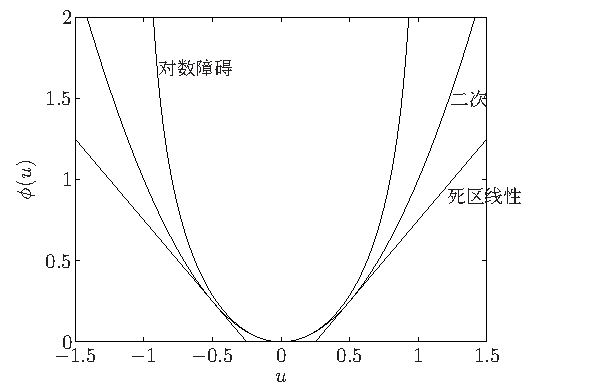
\includegraphics[width=.65\textwidth]{ch06-01.pdf}
\caption*{图6.1\quad 几种常用惩罚函数：二次惩罚函数 $\phi(u)=u^2$、死区宽度为 $a=1/4$ 的死区线性惩罚函数，以及限制值为 $a=1$ 的对数障碍惩罚函数。}
\end{figure}
\begin{origexample}{6.1}
几种常用惩罚函数及其对应的逼近问题。
\begin{itemize}
\item 取 $\phi(u)=|u|^p$，其中 $p\ge1$，惩罚函数逼近问题就等价于 $\ell_p$ 范数逼近问题。特别地，二次惩罚函数 $\phi(u)=u^2$ 给出最小二乘逼近或欧几里得范数逼近；绝对值惩罚函数 $\phi(u)=|u|$ 给出 $\ell_1$ 范数逼近。
\item 死区线性惩罚函数（死区宽度 $a>0$）为
\[\phi(u)=\begin{cases}0,&|u|\le a,\\|u|-a,&|u|>a.\end{cases}\]
对于小于 $a$ 的残差，死区线性函数不施加惩罚。
\item 对数障碍惩罚函数（限制值 $a>0$）为
\[\phi(u)=\begin{cases}-a^2\log\bigl(1-(u/a)^2\bigr),&|u|<a,\\\infty,&|u|\ge a.\end{cases}\]
对于大于 $a$ 的残差，对数障碍惩罚函数施加无穷大的惩罚。
\end{itemize}
图6.1绘出了死区线性、对数障碍和二次惩罚函数。注意，当 $|u/a|\le0.25$ 时，对数障碍函数与二次惩罚非常接近（见习题6.1）。
\end{origexample}

将惩罚函数乘以一个正数，不影响惩罚函数逼近问题的解，因为这只相当于将目标函数作同样缩放。但惩罚函数的形状，会极大地影响惩罚函数逼近问题的解。

% Source PDF page 310 (printed p. 296)
粗略地说，$\phi(u)$ 衡量我们对取值为 $u$ 的残差有多不满意。如果 $u$ 很小时 $\phi(u)$ 也很小（甚至为零），就表示我们对这些取值的残差不太在意（或完全不在意）。如果 $\phi(u)$ 随 $u$ 增大而迅速增长，就表示我们很不希望出现大残差；如果 $\phi$ 在某个区间外取无穷大，则表示该区间之外的残差不可接受。这一简单解释，既有助于理解惩罚函数逼近问题的解，也为选择惩罚函数提供了指引。

例如，比较 $\ell_1$ 范数逼近和 $\ell_2$ 范数逼近，它们的惩罚函数分别为 $\phi_1(u)=|u|$ 和 $\phi_2(u)=u^2$。当 $|u|=1$ 时，两者赋予相同惩罚。对于较小的 $u$，有 $\phi_1(u)\gg\phi_2(u)$，因此与 $\ell_2$ 范数逼近相比，$\ell_1$ 范数逼近对小残差赋予更大的相对权重。对于较大的 $u$，有 $\phi_2(u)\gg\phi_1(u)$，所以 $\ell_1$ 范数逼近对大残差赋予的权重小于 $\ell_2$ 范数逼近。对大、小残差的相对权重不同，会反映在相应逼近问题的解中：与 $\ell_2$ 范数逼近解相比，$\ell_1$ 范数逼近问题的最优残差幅度分布往往包含更多为零或很小的残差。相反，$\ell_2$ 范数解中较大的残差通常相对较少，因为大残差在 $\ell_2$ 范数逼近中的惩罚远大于在 $\ell_1$ 范数逼近中的惩罚。

\subsubsection*{一个例子}
下面用一个例子说明这些想法。取矩阵 $A\in\R^{100\times30}$ 和向量 $b\in\R^{100}$（随机选取，但结果具有代表性），计算 $Ax\approx b$ 的 $\ell_1$、$\ell_2$ 范数近似解，以及采用死区线性惩罚（$a=0.5$）和对数障碍惩罚（$a=1$）的惩罚函数逼近解。图6.2给出了这四种惩罚函数，以及这四种惩罚逼近所对应的最优残差幅度分布。从惩罚函数图可以看出：
\begin{itemize}
\item $\ell_1$ 范数惩罚对小残差赋予的权重最大，对大残差赋予的权重最小。
\item $\ell_2$ 范数惩罚对小残差的权重很小，但对大残差的权重很大。
\item 死区线性惩罚函数不惩罚小于 $0.5$ 的残差，而对大残差也只赋予相对较小的权重。
\item 对数障碍惩罚对小残差的权重与 $\ell_2$ 范数惩罚很接近，但对大于约 $0.8$ 的残差赋予很大权重，对大于 $1$ 的残差则赋予无穷大权重。
\end{itemize}
从幅度分布中可以清楚地看到以下几点：
\begin{itemize}
\item 对 $\ell_1$ 最优解，很多残差为零或非常小；同时它也包含相对更多的大残差。
\end{itemize}

% Source PDF page 311 (printed p. 297)
\begin{figure}[htbp]\centering
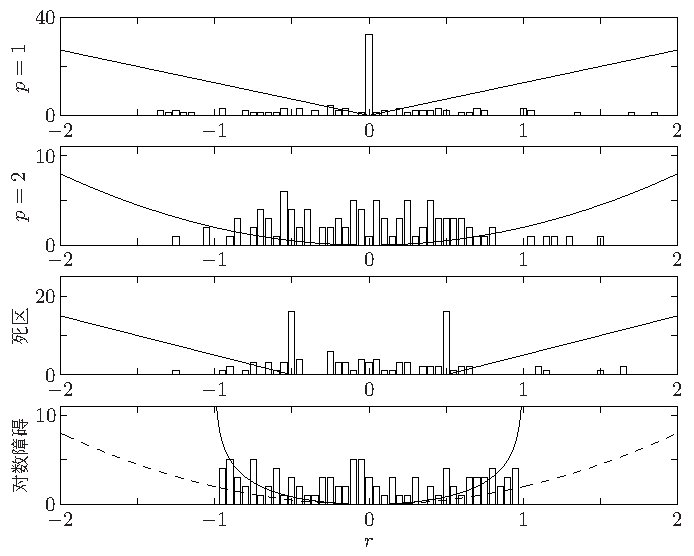
\includegraphics[width=.78\textwidth]{ch06-02.pdf}
\caption*{图6.2\quad 四种惩罚函数对应的残差幅度直方图；图中也绘出了经缩放的惩罚函数以供参考。对数障碍图中还以虚线绘出了二次惩罚函数。}
\end{figure}

% Source PDF page 312 (printed p. 298)
\begin{figure}[htbp]\centering
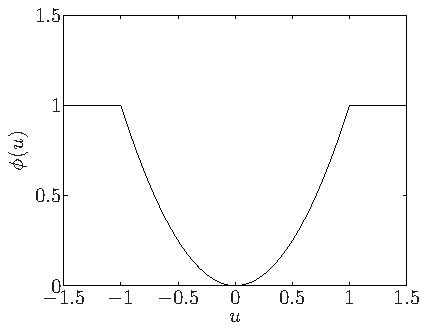
\includegraphics[width=.58\textwidth]{ch06-03.pdf}
\caption*{图6.3\quad 对超过阈值（本例中为 $1$）的残差施加固定惩罚的非凸惩罚函数：当 $|u|\le1$ 时，$\phi(u)=u^2$；当 $|u|>1$ 时，$\phi(u)=1$。因此，用该函数进行惩罚逼近对离群值相对不敏感。}
\end{figure}
\begin{itemize}
\item $\ell_2$ 范数逼近有许多中等大小的残差，而较大的残差相对较少。
\item 对死区线性惩罚，可以看到许多残差的值为 $\pm0.5$，恰好落在不受惩罚的“免费”区域边缘。
\item 对对数障碍惩罚，没有残差的幅度大于 $1$；除此之外，其残差分布与 $\ell_2$ 范数逼近的残差分布相似。
\end{itemize}

\subsubsection*{对离群值或大误差的敏感性}
在估计或回归问题中，\emph{离群值}是噪声 $v_i$ 相对较大的测量值 $y_i=a_i^\T x+v_i$。它常与错误数据或有缺陷的测量有关。存在离群值时，对 $x$ 的任何估计所对应的残差向量中，都会有一些较大的分量。理想情况下，希望能判断哪些测量是离群值，把它们从估计过程中剔除，或者大幅降低它们在估计中的权重。（不过，不能对很大的残差赋予零惩罚，否则最优点很可能会使所有残差都很大，从而使总惩罚为零。）可以使用惩罚函数逼近，并采用如下惩罚函数来实现这一想法：
\begin{equation}
\phi(u)=\begin{cases}u^2,&|u|\le M,\\M^2,&|u|>M,\end{cases}\tag{6.3}
\end{equation}
如图6.3所示。对于小于 $M$ 的残差，该惩罚函数与最小二乘一致；但对大于 $M$ 的残差，无论究竟大多少，都施加固定惩罚。也就是说，超过 $M$ 的残差被忽略，假定它们来自离群值或错误数据。遗憾的是，惩罚函数 (6.3) 非凸，相应的惩罚函数逼近问题会变成困难的组合优化问题。

% Source PDF page 313 (printed p. 299)
\begin{figure}[htbp]\centering
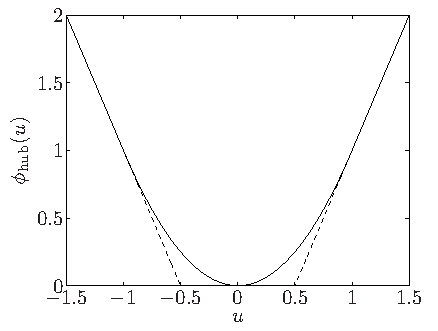
\includegraphics[width=.58\textwidth]{ch06-04.pdf}
\caption*{图6.4\quad 实线是取 $M=1$ 的稳健最小二乘惩罚函数，即 Huber 惩罚函数 $\phi_{\rm hub}$。当 $|u|\le M$ 时它是二次的，当 $|u|>M$ 时呈线性增长。}
\end{figure}
基于惩罚函数的估计方法对离群值的敏感程度，取决于惩罚函数对大残差所赋予的相对惩罚。如果只考虑会产生凸优化问题的凸惩罚函数，那么对离群值最不敏感的，是在 $u$ 较大时像 $|u|$ 那样线性增长的 $\phi(u)$。具有这一性质的惩罚函数有时称为\emph{稳健}的，因为相应的惩罚函数逼近方法对离群值或大误差的敏感性，比最小二乘等方法低得多。

一个显然的稳健惩罚函数是 $\phi(u)=|u|$，它对应 $\ell_1$ 范数逼近。另一个例子是\emph{稳健最小二乘}惩罚函数，即 \emph{Huber 惩罚函数}：
\begin{equation}
\phi_{\rm hub}(u)=\begin{cases}u^2,&|u|\le M,\\M(2|u|-M),&|u|>M,\end{cases}\tag{6.4}
\end{equation}
如图6.4所示。对于小于 $M$ 的残差，该惩罚函数与最小二乘惩罚函数一致；对较大的残差，则转为类似 $\ell_1$ 范数的线性增长。Huber 惩罚函数可以在下述意义下看作离群惩罚函数 (6.3) 的凸近似：当 $|u|\le M$ 时，两者相同；当 $|u|>M$ 时，Huber 惩罚函数是与离群惩罚函数 (6.3) 最接近的凸函数。

\begin{origexample}{6.2}
\emph{稳健回归。}图6.5给出了平面上的42个点 $(t_i,y_i)$，其中有两个明显的离群值（一个在左上方，另一个在右下方）。虚线是用直线 $f(t)=\alpha+\beta t$ 对这些点作最小二乘逼近的结果。系数 $\alpha$、$\beta$ 由下述最小二乘问题得到：
\[\text{最小化}\quad\sum_{i=1}^{42}(y_i-\alpha-\beta t_i)^2,\]
变量为 $\alpha$ 和 $\beta$。最小二乘逼近直线明显偏离了这些点主要分布的方向，转向了两个离群值。

% Source PDF page 314 (printed p. 300)
\begin{figure}[htbp]\centering
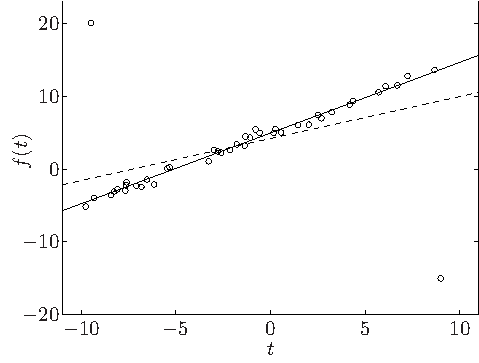
\includegraphics[width=.62\textwidth]{ch06-05.pdf}
\caption*{图6.5\quad 图中的42个圆圈表示可由仿射函数很好逼近的点，但左上方和右下方两个离群值例外。虚线是直线 $f(t)=\alpha+\beta t$ 的最小二乘拟合，它偏离了点的主要分布方向，转向离群值。实线是最小化 $M=1$ 的 Huber 惩罚函数所得到的稳健最小二乘拟合；它对非离群数据的拟合好得多。}
\end{figure}
实线是最小化 Huber 惩罚函数
\[\text{最小化}\quad\sum_{i=1}^{42}\phi_{\rm hub}(y_i-\alpha-\beta t_i),\]
所得到的稳健最小二乘逼近，其中 $M=1$。这个逼近受离群值的影响小得多。
\end{origexample}

由于 $\ell_1$ 范数逼近是各种凸惩罚函数逼近方法中对离群值最稳健的方法之一，它有时称为\emph{稳健估计}或\emph{稳健回归}。$\ell_1$ 范数估计的稳健性也可以从统计框架理解；见第353页。

\subsubsection*{小残差与 $\ell_1$ 范数逼近}
也可以把注意力放在小残差上。最小二乘逼近对小残差赋予的权重很小，因为当 $u$ 很小时，$\phi(u)=u^2$ 非常小。死区线性惩罚函数等对小残差的惩罚为零。对于在残差较小时取值非常小的惩罚函数，可以预期最优残差会比较小，但不会非常小。粗略地说，把一个已经很小的残差继续缩小，几乎或完全没有收益。

相反，$\phi(u)=|u|$ 这类对小残差赋予较大相对权重的惩罚函数，对应于 $\ell_1$ 范数逼近，往往会产生大量非常小、甚至恰好为零的最优残差。这意味着，在 $\ell_1$ 范数逼近中，通常会发现许多方程被精确满足，即对许多 $i$ 有 $a_i^\T x=b_i$。这一现象可以从图6.2看到。

% Source PDF page 315 (printed p. 301)
\subsection{带约束的逼近}
可以在基本范数逼近问题 (6.1) 中加入约束。若这些约束是凸的，所得到的问题也是凸问题。约束可能出于多种原因。
\begin{itemize}
\item 在逼近问题中，可以用约束排除某些不可接受的向量 $b$ 的近似，或者保证逼近向量 $Ax$ 满足某些性质。
\item 在估计问题中，约束来自对待估向量 $x$ 的先验知识，或者对估计误差 $v$ 的先验知识。
\item 在几何问题中，要确定点 $b$ 在比子空间更复杂的集合（例如锥或多面体）上的投影，也会产生约束。
\end{itemize}
下面用几个例子说明。

\subsubsection*{变量的非负约束}
在基本范数逼近问题中加入约束 $x\succeq0$：
\[\begin{array}{ll}\text{最小化}&\norm{Ax-b}\\\text{约束条件}&x\succeq0.\end{array}\]
在估计中，如果已知待估参数向量 $x$ 的分量非负，例如功率、强度或速率，就会有非负约束。几何上，这是确定向量 $b$ 到由 $A$ 的列生成的锥的投影。也可以把该问题解释为用 $A$ 的列的非负线性组合（即锥组合）逼近 $b$。

\subsubsection*{变量界}
这里加入约束 $l\preceq x\preceq u$，其中 $l,u\in\R^n$ 是问题参数：
\[\begin{array}{ll}\text{最小化}&\norm{Ax-b}\\\text{约束条件}&l\preceq x\preceq u.\end{array}\]
在估计中，变量界来自预先知道的各变量所在区间。几何上，这是求向量 $b$ 到一个盒在由 $A$ 定义的线性映射下的像的投影。

% Source PDF page 316 (printed p. 302)
\subsubsection*{概率分布}
可以要求 $x$ 满足 $x\succeq0$、$\one^\T x=1$：
\[\begin{array}{ll}\text{最小化}&\norm{Ax-b}\\\text{约束条件}&x\succeq0,\quad\one^\T x=1.\end{array}\]
在估计比例或相对频率时会有这样的约束，因为它们非负且总和为 $1$。这也可以解释为用 $A$ 的列的凸组合逼近 $b$。（第7.2节将详细讨论概率估计。）

\subsubsection*{范数球约束}
可以在基本范数逼近问题中加入 $x$ 位于某个范数球内的约束：
\[\begin{array}{ll}\text{最小化}&\norm{Ax-b}\\\text{约束条件}&\norm{x-x_0}\le d,\end{array}\]
其中 $x_0$ 和 $d$ 是问题参数。加入这一约束有以下几种理由。
\begin{itemize}
\item 在估计中，$x_0$ 是对参数 $x$ 的先验猜测，$d$ 是我们认为估计相对于先验猜测可能偏离的最大幅度。参数 $x$ 的估计值 $\widehat x$，是在所有可信候选值（满足 $\norm{z-x_0}\le d$ 的 $z$）中，与测量数据最匹配的值，即使 $\norm{Az-b}$ 最小的值。
\item 约束 $\norm{x-x_0}\le d$ 可以表示一个\emph{信赖域}。这里，线性关系 $y=Ax$ 只是某个非线性关系 $y=f(x)$ 的近似；仅当 $x$ 靠近某点 $x_0$，具体说满足 $\norm{x-x_0}\le d$ 时，这一近似才成立。问题要在模型 $y=Ax$ 可信的那些 $x$ 中最小化 $\norm{Ax-b}$。
\end{itemize}
这些想法也会在正则化中出现，见第6.3.2节。

\section{最小范数问题}
基本的最小范数问题为
\begin{equation}
\begin{array}{ll}\text{最小化}&\norm x\\\text{约束条件}&Ax=b,\end{array}\tag{6.5}
\end{equation}
其中数据为 $A\in\R^{m\times n}$、$b\in\R^m$，变量为 $x\in\R^n$，$\norm{\cdot}$ 是 $\R^n$ 上的一个范数。只要线性方程 $Ax=b$ 有解，该问题的解就一定存在，称为 $Ax=b$ 的\emph{最小范数解}。最小范数问题当然是凸优化问题。

不失一般性，可以假设 $A$ 的行线性无关，因此 $m\le n$。当 $m=n$ 时，唯一可行点为 $x=A^{-1}b$；只有当 $m<n$，即方程 $Ax=b$ 是欠定方程时，最小范数问题才有意义。

% Source PDF page 317 (printed p. 303)
\subsubsection*{改写为范数逼近问题}
通过消去等式约束，可以将最小范数问题 (6.5) 写成范数逼近问题。令 $x_0$ 为 $Ax=b$ 的任意一个解，$Z\in\R^{n\times k}$ 的列构成 $A$ 的零空间的一组基。那么，$Ax=b$ 的通解为 $x_0+Zu$，其中 $u\in\R^k$。最小范数问题 (6.5) 可以写成
\[\text{最小化}\quad\norm{x_0+Zu},\]
变量为 $u\in\R^k$；这是一个范数逼近问题。特别地，对范数逼近问题的分析与讨论，作适当解释后，也同样适用于最小范数问题。

\subsubsection*{控制或设计解释}
最小范数问题 (6.5) 可以解释为最优设计或最优控制问题。$n$ 个变量 $x_1,\ldots,x_n$ 是待确定取值的设计变量。在控制中，这些变量表示要选择取值的输入。向量 $y=Ax$ 给出设计 $x$ 的 $m$ 个属性或结果，假定它们是设计变量 $x$ 的线性函数。$m<n$ 个方程 $Ax=b$ 表示对设计的 $m$ 项指标或要求。由于 $m<n$，这些要求尚未完全确定设计；设计中还有 $n-m$ 个自由度（假设 $A$ 的秩为 $m$）。

在所有满足指标的设计中，最小范数问题选择按 $\norm{\cdot}$ 衡量最小的设计。这可以看作最高效的设计：它用尽可能小的 $x$ 达到指标 $Ax=b$。

\subsubsection*{估计解释}
假设 $x$ 是待估计的参数向量。我们有 $m<n$ 个完全精确、没有噪声的线性测量 $Ax=b$。由于测量数少于待估参数数，测量不能完全确定 $x$。任何满足 $Ax=b$ 的参数向量 $x$ 都与测量一致。

要在不增加测量的情况下合理猜测 $x$，必须使用先验信息。假设先验信息或假设是：按 $\norm{\cdot}$ 衡量，$x$ 更可能较小而非较大。最小范数问题就在所有与测量 $Ax=b$ 一致的参数向量中，选择最小、因而最可信的一个作为估计。（最小范数问题的统计解释见第359页。）

\subsubsection*{几何解释}
最小范数问题 (6.5) 也有一个简单的几何解释。可行集 $\{x\mid Ax=b\}$ 是仿射集，目标是 $x$ 到原点的距离（以 $\norm{\cdot}$ 衡量）。最小范数问题寻找该仿射集中距离原点最近的点，即确定原点到仿射集 $\{x\mid Ax=b\}$ 的投影。

% Source PDF page 318 (printed p. 304)
\subsubsection*{线性方程的最小二乘解}
最常见的最小范数问题使用欧几里得范数，即 $\ell_2$ 范数。将目标平方，得到等价问题
\[\begin{array}{ll}\text{最小化}&\norm x_2^2\\\text{约束条件}&Ax=b,\end{array}\]
其唯一解称为方程 $Ax=b$ 的\emph{最小二乘解}。与最小二乘逼近问题一样，该问题也可解析求解。引入对偶变量 $\nu\in\R^m$，最优性条件为
\[2x^\star+A^\T\nu^\star=0,\qquad Ax^\star=b,\]
这是一组容易求解的线性方程。从第一个方程得到 $x^\star=-(1/2)A^\T\nu^\star$，代入第二个方程得到 $-(1/2)AA^\T\nu^\star=b$，从而
\[\nu^\star=-2(AA^\T)^{-1}b,\qquad x^\star=A^\T(AA^\T)^{-1}b.\]
（由于 $\rank A=m<n$，矩阵 $AA^\T$ 可逆。）

\subsubsection*{最小惩罚问题}
最小范数问题 (6.5) 的一种有用变体是\emph{最小惩罚问题}
\begin{equation}
\begin{array}{ll}\text{最小化}&\phi(x_1)+\cdots+\phi(x_n)\\\text{约束条件}&Ax=b,\end{array}\tag{6.6}
\end{equation}
其中 $\phi:\R\to\R$ 是凸且非负的函数，并满足 $\phi(0)=0$。惩罚函数值 $\phi(u)$ 量化我们对 $x$ 的某个分量取值为 $u$ 的不满意程度；最小惩罚问题则在约束 $Ax=b$ 下，寻找总惩罚最小的 $x$。

惩罚函数逼近中关于惩罚函数的全部讨论与解释，都可以移用于最小惩罚问题，只需将惩罚逼近问题中残差 $r$ 的幅度分布，换成最小惩罚问题中 $x$ 的幅度分布。

\subsubsection*{用最小 $\ell_1$ 范数获得稀疏解}
回顾第300页的讨论，$\ell_1$ 范数逼近对小残差赋予较大相对权重，因此许多最优残差会很小，甚至为零。最小范数问题中也会出现类似现象。最小 $\ell_1$ 范数问题
\[\begin{array}{ll}\text{最小化}&\norm x_1\\\text{约束条件}&Ax=b\end{array}\]
往往产生有大量零分量的解 $x$。换言之，最小 $\ell_1$ 范数问题倾向于产生 $Ax=b$ 的稀疏解，非零分量常有 $m$ 个。

% Source PDF page 319 (printed p. 305)
很容易找到只有 $m$ 个非零分量的 $Ax=b$ 的解。从 $1,\ldots,n$ 中任选 $m$ 个指标，作为 $x$ 的非零分量所在位置。方程 $Ax=b$ 就化为 $\widetilde A\widetilde x=b$，其中 $\widetilde A$ 是从 $A$ 中取相应列得到的 $m\times m$ 子矩阵，$\widetilde x\in\R^m$ 是由选定的 $m$ 个分量构成的 $x$ 的子向量。若 $\widetilde A$ 非奇异，可取 $\widetilde x=\widetilde A^{-1}b$，得到一个非零分量不超过 $m$ 个的可行解 $x$。若 $\widetilde A$ 奇异且 $b\notin\mathcal R(\widetilde A)$，则 $\widetilde A\widetilde x=b$ 无解，意味着在选定的非零位置上没有可行的 $x$。若 $\widetilde A$ 奇异且 $b\in\mathcal R(\widetilde A)$，则存在非零分量少于 $m$ 个的可行解。

这种方法可以寻找具有 $m$ 个或更少非零分量的最小 $x$，但通常需要检查并比较从 $x$ 的 $n$ 个系数中选择 $m$ 个非零系数的全部 $n!/[m!(n-m)!]$ 种可能。相比之下，求解最小 $\ell_1$ 范数问题，是寻找 $Ax=b$ 的稀疏且较小的解的一种良好启发式方法。

\section{正则化逼近}
\subsection{双准则表述}
正则化逼近的基本目标，是寻找一个尽可能小、同时也使残差 $Ax-b$ 小的向量 $x$。自然地，这可以表述为一个具有 $\norm{Ax-b}$ 和 $\norm x$ 两个目标的凸向量优化问题：
\begin{equation}
\text{相对于 }\R_+^2\text{ 最小化}\quad(\norm{Ax-b},\norm x).\tag{6.7}
\end{equation}
两个范数可以不同：第一个定义在 $\R^m$ 上，衡量残差大小；第二个定义在 $\R^n$ 上，衡量 $x$ 的大小。

两个目标之间的最优权衡可以通过多种方法求得，然后绘出 $\norm{Ax-b}$ 与 $\norm x$ 的最优权衡曲线；它表明，要使一个目标较小，另一个目标至少必须多大。$\norm{Ax-b}$ 与 $\norm x$ 的最优权衡曲线的一个端点容易描述。$\norm x$ 的最小值是零，仅在 $x=0$ 时取得；此时残差范数为 $\norm b$。

权衡曲线的另一个端点较复杂。令 $C$ 表示 $\norm{Ax-b}$ 的最小化点集合（对 $\norm x$ 不加约束）。那么，$C$ 中任意一个最小范数点都是 Pareto 最优点，对应权衡曲线的另一个端点。也就是说，这个端点对应的 Pareto 最优点，是使 $\norm{Ax-b}$ 最小的所有点中的最小范数点。如果两个范数都是欧几里得范数，该 Pareto 最优点唯一，为 $x=A^\dagger b$，其中 $A^\dagger$ 是 $A$ 的伪逆。（见第4.7.6节，第184页，以及第A.5.4节。）

% Source PDF page 320 (printed p. 306)
\subsection{正则化}
\emph{正则化}是求解双准则问题 (6.7) 常用的一种标量化方法。一种正则化形式是最小化两个目标的加权和：
\begin{equation}\text{最小化}\quad\norm{Ax-b}+\gamma\norm x,\tag{6.8}\end{equation}
其中 $\gamma>0$ 是问题参数。当 $\gamma$ 在 $(0,\infty)$ 上变化时，问题 (6.8) 的解描绘出最优权衡曲线。

另一种常用正则化方法，尤其在使用欧几里得范数时，是对不同的 $\delta>0$，最小化范数平方的加权和，即
\begin{equation}\text{最小化}\quad\norm{Ax-b}^2+\delta\norm x^2.\tag{6.9}\end{equation}
这些正则化逼近问题通过增加一个与 $x$ 的范数有关的附加项或惩罚项，求解同时使 $\norm{Ax-b}$ 和 $\norm x$ 较小的双准则问题。

\subsubsection*{解释}
正则化用于多种场合。在估计中，惩罚较大 $\norm x$ 的附加项可以解释为：先验知识认为 $\norm x$ 不会太大。在最优设计中，附加项把使用较大设计变量所带来的代价，加入偏离目标指标的代价。

要求 $\norm x$ 较小，也可能来自建模问题。例如，$y=Ax$ 可能只是 $x$ 与 $y$ 的真实关系 $y=f(x)$ 的良好近似。要有 $f(x)\approx b$，既希望 $Ax\approx b$，也需要 $x$ 较小，以保证 $f(x)\approx Ax$。

第6.4.1节和第6.4.2节将说明，正则化可以用来考虑矩阵 $A$ 的变化。粗略地说，较大的 $x$ 会使 $A$ 的变化导致 $Ax$ 的较大变化，因此应避免。

当矩阵 $A$ 是方阵、目标是求解线性方程 $Ax=b$ 时，也可以采用正则化。如果 $A$ 病态甚至奇异，正则化就在解方程（使 $\norm{Ax-b}$ 为零）与把 $x$ 保持在合理大小之间作出折中。

正则化也会出现在统计问题中；见第7.1.2节。

\subsubsection*{Tikhonov 正则化}
最常见的正则化形式基于式 (6.9)，并采用欧几里得范数，得到一个凸二次优化问题：
\begin{equation}
\begin{split}
\text{最小化}\quad&\norm{Ax-b}_2^2+\delta\norm x_2^2\\
&=x^\T(A^\T A+\delta I)x-2b^\T Ax+b^\T b.
\end{split}\tag{6.10}
\end{equation}
这个 Tikhonov 正则化问题具有解析解
\[x=(A^\T A+\delta I)^{-1}A^\T b.\]
由于任意 $\delta>0$ 都有 $A^\T A+\delta I\succ0$，Tikhonov 正则化最小二乘解不需要对矩阵 $A$ 的秩或维数作任何假设。

% Source PDF page 321 (printed p. 307)
\subsubsection*{平滑正则化}
正则化的想法，即在目标中增加一个惩罚较大 $x$ 的项，可以从几个方面推广。一种有用推广是把正则项 $\norm x$ 换为 $\norm{Dx}$。在许多应用中，矩阵 $D$ 表示近似微分算子或二阶微分算子，因此 $\norm{Dx}$ 衡量 $x$ 的变化或平滑程度。

例如，假设向量 $x\in\R^n$ 表示某个连续物理参数（如温度）沿区间 $[0,1]$ 的取值：$x_i$ 是点 $i/n$ 处的温度。该参数在 $i/n$ 附近的梯度或一阶导数，可简单近似为 $n(x_{i+1}-x_i)$；二阶导数的简单近似为二阶差分
\[n\bigl(n(x_{i+1}-x_i)-n(x_i-x_{i-1})\bigr)=n^2(x_{i+1}-2x_i+x_{i-1}).\]
若 $\Delta$ 是如下三对角 Toeplitz 矩阵
\[
\Delta=n^2\begin{bmatrix}
1&-2&1&0&\cdots&0&0&0&0\\
0&1&-2&1&\cdots&0&0&0&0\\
0&0&1&-2&\cdots&0&0&0&0\\
\vdots&\vdots&\vdots&\vdots&&\vdots&\vdots&\vdots&\vdots\\
0&0&0&0&\cdots&1&-2&1&0\\
0&0&0&0&\cdots&0&1&-2&1
\end{bmatrix}\in\R^{(n-2)\times n},
\]
那么 $\Delta x$ 就近似表示该参数的二阶导数，所以 $\norm{\Delta x}_2^2$ 衡量该参数在 $[0,1]$ 上的均方曲率。

Tikhonov 正则化问题
\[\text{最小化}\quad\norm{Ax-b}_2^2+\delta\norm{\Delta x}_2^2\]
可以在两个目标之间进行权衡：$\norm{Ax-b}_2$ 可以衡量拟合程度或与实验数据的一致程度，$\norm{\Delta x}_2$ 则近似表示背后物理参数的均方曲率。参数 $\delta$ 用于控制所需的正则化程度，或绘出拟合程度与平滑程度之间的最优权衡曲线。

还可以增加多个正则项。例如，同时加入与平滑程度和大小有关的项：
\[\text{最小化}\quad\norm{Ax-b}_2^2+\delta\norm{\Delta x}_2^2+\eta\norm x_2^2.\]
其中参数 $\delta\ge0$ 控制近似解的平滑程度，参数 $\eta\ge0$ 控制其大小。

\begin{origexample}{6.3}
\emph{最优输入设计。}考虑一个动态系统，标量输入序列为 $u(0),u(1),\ldots,u(N)$，标量输出序列为 $y(0),y(1),\ldots,y(N)$，两者通过卷积相联系：
\[y(t)=\sum_{\tau=0}^t h(\tau)u(t-\tau),\qquad t=0,1,\ldots,N.\]

% Source PDF page 322 (printed p. 308)
序列 $h(0),h(1),\ldots,h(N)$ 称为系统的卷积核或冲激响应。

我们的目标是选择输入序列 $u$，以达到几个目标。
\begin{itemize}
\item \emph{输出跟踪。}首要目标是使输出 $y$ 跟踪、跟随一个给定的目标或参考信号 $y_{\rm des}$。用二次函数
\[J_{\rm track}=\frac1{N+1}\sum_{t=0}^N(y(t)-y_{\rm des}(t))^2\]
衡量输出跟踪误差。
\item \emph{小输入。}输入不应太大。用二次函数
\[J_{\rm mag}=\frac1{N+1}\sum_{t=0}^N u(t)^2\]
衡量输入的大小。
\item \emph{小输入变化。}输入不应变化过快。用二次函数
\[J_{\rm der}=\frac1N\sum_{t=0}^{N-1}(u(t+1)-u(t))^2\]
衡量输入变化的大小。
\end{itemize}
最小化加权和
\[J_{\rm track}+\delta J_{\rm der}+\eta J_{\rm mag},\]
其中 $\delta>0$、$\eta>0$，就可以在三个目标之间权衡。

下面考虑一个具体例子，其中 $N=200$，冲激响应为
\[h(t)=\frac19(0.9)^t(1-0.4\cos(2t)).\]
图6.6给出三组正则化参数 $\delta$、$\eta$ 下的最优输入及相应输出（同时绘出期望轨迹 $y_{\rm des}$）。第一行是 $\delta=0$、$\eta=0.005$ 时的最优输入和输出。这时对输入大小作了一定正则化，但没有对其变化作正则化。虽然跟踪良好，即 $J_{\rm track}$ 很小，但所需输入很大，且变化迅速。第二行对应 $\delta=0$、$\eta=0.05$。此时对输入大小施加了更强正则化，仍未对 $u$ 的变化作正则化。对应输入确实变小了，代价是跟踪误差增大。最后一行是 $\delta=0.3$、$\eta=0.05$ 的结果。此时增加了对输入变化的正则化，输入变化大幅减小，而输出跟踪误差并未增加很多。
\end{origexample}

\subsubsection*{$\ell_1$ 范数正则化}
$\ell_1$ 范数正则化可以作为寻找稀疏解的启发式方法。例如，考虑问题
\begin{equation}\text{最小化}\quad\norm{Ax-b}_2+\gamma\norm x_1,\tag{6.11}\end{equation}
其中残差以欧几里得范数衡量，而正则化使用 $\ell_1$ 范数。

% Source PDF page 323 (printed p. 309)
\begin{figure}[htbp]\centering
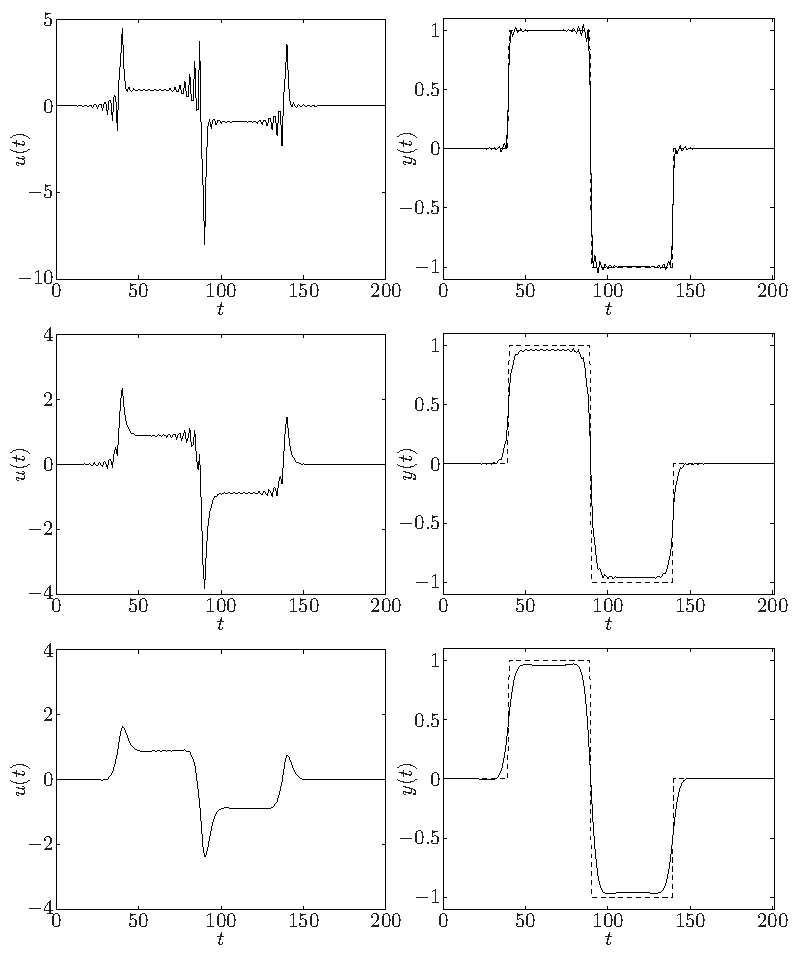
\includegraphics[width=.9\textwidth]{ch06-06.pdf}
\caption*{图6.6\quad 三组正则化参数下的最优输入（左）及相应输出（右）。$\delta$ 对应输入变化，$\eta$ 对应输入大小。右侧各图中的虚线是期望输出 $y_{\rm des}$。第一行：$\delta=0$、$\eta=0.005$；第二行：$\delta=0$、$\eta=0.05$；最后一行：$\delta=0.3$、$\eta=0.05$。}
\end{figure}

% Source PDF page 324 (printed p. 310)
改变参数 $\gamma$，就能描绘 $\norm{Ax-b}_2$ 与 $\norm x_1$ 之间的最优权衡曲线；它近似表示 $\norm{Ax-b}_2$ 与向量 $x$ 的稀疏程度或基数 $\operatorname{card}(x)$（即非零元素数）之间的最优权衡曲线。问题 (6.11) 可以改写为 SOCP 并求解。

\begin{origexample}{6.4}
\emph{回归向量选择问题。}给定矩阵 $A\in\R^{m\times n}$，其各列是候选回归向量；还有向量 $b\in\R^m$，要用 $A$ 的 $k<n$ 列的线性组合拟合它。问题是选择所用的 $k$ 个回归向量以及相应系数。可写成
\[\begin{array}{ll}\text{最小化}&\norm{Ax-b}_2\\\text{约束条件}&\operatorname{card}(x)\le k.\end{array}\]
一般而言，这是一个困难的组合问题。

一种直接方法是逐一检查 $x$ 的所有具有 $k$ 个非零元素的稀疏模式。固定稀疏模式后，可通过最小二乘问题求最优 $x$，即最小化 $\norm{\widetilde A\widetilde x-b}_2$，其中 $\widetilde A$ 是保留与该模式对应的列得到的 $A$ 的子矩阵，$\widetilde x$ 是由 $x$ 的非零分量构成的子向量。对全部 $n!/[k!(n-k)!]$ 种含 $k$ 个非零元素的稀疏模式，都进行这项计算。

一种良好启发式方法，是对不同 $\gamma$ 求解问题 (6.11)，找出使解满足 $\operatorname{card}(x)=k$ 的最小 $\gamma$，随后固定这个稀疏模式，寻找使 $\norm{Ax-b}_2$ 最小的 $x$。

图6.7给出一个数值例子，其中 $A\in\R^{10\times20}$、$x\in\R^{20}$、$b\in\R^{10}$。虚线上的圆圈是 $\operatorname{card}(x)$（纵轴）与残差 $\norm{Ax-b}_2$（横轴）之间权衡的全局 Pareto 最优值。对每个 $k$，均按上述方法枚举具有 $k$ 个非零元素的全部稀疏模式，得到 Pareto 最优点。实线上的圆圈则来自启发式方法，采用不同 $\gamma$ 下问题 (6.11) 的解所具有的稀疏模式。注意，当 $\operatorname{card}(x)=1$ 时，启发式方法确实找到了全局最优解。

基追踪（第6.5.4节）还会用到这个想法。
\end{origexample}

\subsection{重构、平滑与去噪}
本节介绍上述双准则逼近问题的一个重要特例，并用例子说明不同正则化方法的表现。重构问题从一个以向量 $x\in\R^n$ 表示的信号出发。系数 $x_i$ 对应某个时间函数在等间距点上的取值（用信号处理术语，就是采样值）。通常假设信号不会变化太快，也就是一般有 $x_i\approx x_{i+1}$。（本节考虑一维信号，如音频信号；同样的思想也适用于二维或更高维信号，如图像或视频。）

% Source PDF page 325 (printed p. 311)
\begin{figure}[htbp]\centering
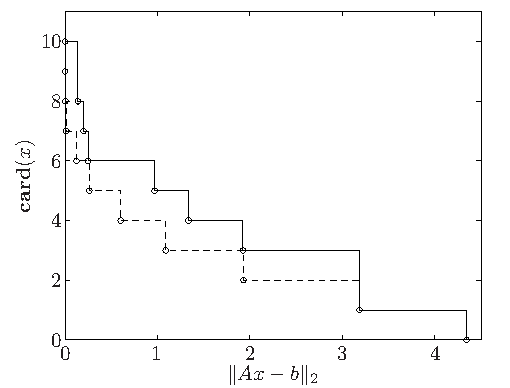
\includegraphics[width=.65\textwidth]{ch06-07.pdf}
\caption*{图6.7\quad 对矩阵 $A\in\R^{10\times20}$ 进行稀疏回归向量选择。虚线上的圆圈，是残差 $\norm{Ax-b}_2$ 与非零元素数 $\operatorname{card}(x)$ 之间权衡的 Pareto 最优值。实线上以圆圈标出的点，由 $\ell_1$ 范数正则化启发式方法得到。}
\end{figure}
信号 $x$ 被加性噪声 $v$ 污染：
\[x_{\rm cor}=x+v.\]
噪声可以用许多不同方式建模，这里只假定它未知、较小，并且与信号不同，它变化迅速。目标是给定受污染信号 $x_{\rm cor}$，构造原信号 $x$ 的估计 $\widehat x$。这个过程称为\emph{信号重构}，因为要从受污染的版本中重构原信号；也称为\emph{去噪}，因为要从受污染的信号中除去噪声。大多数重构方法最终都会对 $x_{\rm cor}$ 作某种平滑操作而得到 $\widehat x$，因此这个过程也称为\emph{平滑}。

重构问题的一种简单表述是双准则问题
\begin{equation}
\text{相对于 }\R_+^2\text{ 最小化}\quad(\norm{\widehat x-x_{\rm cor}}_2,\phi(\widehat x)),\tag{6.12}
\end{equation}
其中 $\widehat x$ 是变量，$x_{\rm cor}$ 是问题参数。函数 $\phi:\R^n\to\R$ 是凸函数，称为\emph{正则化函数}或\emph{平滑目标}，用于衡量估计 $\widehat x$ 的粗糙程度或不平滑程度。重构问题 (6.12) 寻找与受污染信号接近（按 $\ell_2$ 范数衡量）、同时又平滑（$\phi(\widehat x)$ 较小）的信号。问题 (6.12) 是凸双准则问题，可以通过标量化并求解一个标量凸优化问题，得到 Pareto 最优点。

% Source PDF page 326 (printed p. 312)
\subsubsection*{二次平滑}
最简单的重构方法采用二次平滑函数
\[\phi_{\rm quad}(x)=\sum_{i=1}^{n-1}(x_{i+1}-x_i)^2=\norm{Dx}_2^2,\]
其中 $D\in\R^{(n-1)\times n}$ 是双对角矩阵
\[D=\begin{bmatrix}-1&1&0&\cdots&0&0&0\\0&-1&1&\cdots&0&0&0\\\vdots&\vdots&\vdots&&\vdots&\vdots&\vdots\\0&0&0&\cdots&-1&1&0\\0&0&0&\cdots&0&-1&1\end{bmatrix}.\]
通过最小化
\[\norm{\widehat x-x_{\rm cor}}_2^2+\delta\norm{D\widehat x}_2^2,\]
可以得到 $\norm{\widehat x-x_{\rm cor}}_2$ 与 $\norm{D\widehat x}_2$ 的最优权衡，其中 $\delta>0$ 将最优权衡曲线参数化。该二次问题的解为
\[\widehat x=(I+\delta D^\T D)^{-1}x_{\rm cor}.\]
由于 $I+\delta D^\T D$ 是三对角矩阵，这个解可以非常高效地计算，见附录C。

\subsubsection*{二次平滑的例子}
图6.8给出信号 $x\in\R^{4000}$（上）及受污染信号 $x_{\rm cor}$（下）。目标 $\norm{\widehat x-x_{\rm cor}}_2$ 与 $\norm{D\widehat x}_2$ 的最优权衡曲线见图6.9。曲线最左端对应 $\widehat x=x_{\rm cor}$，目标值为 $\norm{Dx_{\rm cor}}_2=4.4$；最右端对应 $\widehat x=0$，此时 $\norm{\widehat x-x_{\rm cor}}_2=\norm{x_{\rm cor}}_2=16.2$。注意，曲线在 $\norm{\widehat x-x_{\rm cor}}_2\approx3$ 附近有明显拐弯。

图6.10给出最优权衡曲线上的三个平滑信号，分别对应 $\norm{\widehat x-x_{\rm cor}}_2=8$（上）、$3$（中）和 $1$（下）。把重构信号与原信号 $x$ 比较，可见 $\norm{\widehat x-x_{\rm cor}}_2=3$ 时的重构最好，正对应权衡曲线的拐弯处。$\norm{\widehat x-x_{\rm cor}}_2$ 更大时，平滑过度；更小时，平滑不足。

\subsubsection*{全变差重构}
当原信号十分平滑，而噪声变化迅速时，简单的二次平滑是一种很好的重构方法。但显然，原信号中的任何快速变化也都会被二次平滑削弱或消除。本节介绍一种既能消除大部分噪声，又能保留原信号中偶尔出现的快速变化的重构方法。该方法基于平滑函数
\[\phi_{\rm tv}(\widehat x)=\sum_{i=1}^{n-1}|\widehat x_{i+1}-\widehat x_i|=\norm{D\widehat x}_1,\]
它称为 $x\in\R^n$ 的\emph{全变差}。

% Source PDF page 327 (printed p. 313)
\begin{figure}[htbp]\centering
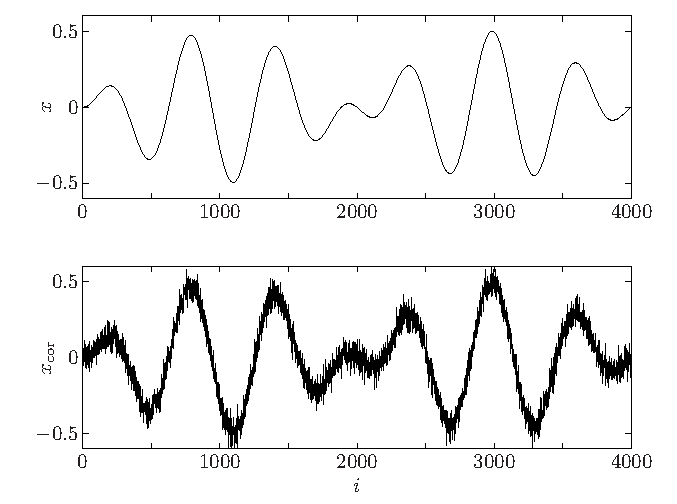
\includegraphics[width=.85\textwidth]{ch06-08.pdf}
\caption*{图6.8\quad 上：原信号 $x\in\R^{4000}$。下：受污染信号 $x_{\rm cor}$。}
\end{figure}
\begin{figure}[htbp]\centering
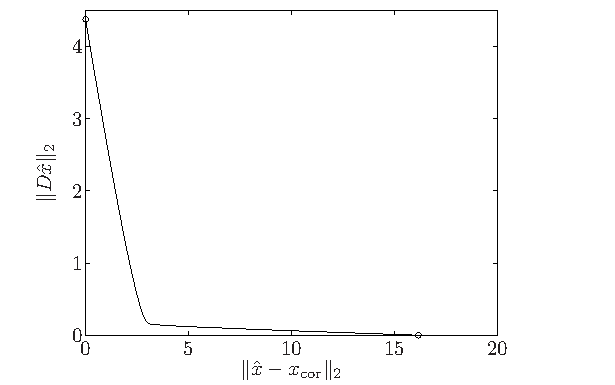
\includegraphics[width=.65\textwidth]{ch06-09.pdf}
\caption*{图6.9\quad $\norm{D\widehat x}_2$ 与 $\norm{\widehat x-x_{\rm cor}}_2$ 之间的最优权衡曲线。在 $\norm{\widehat x-x_{\rm cor}}\approx3$ 附近，曲线有明显拐弯。}
\end{figure}

% Source PDF page 328 (printed p. 314)
\begin{figure}[htbp]\centering
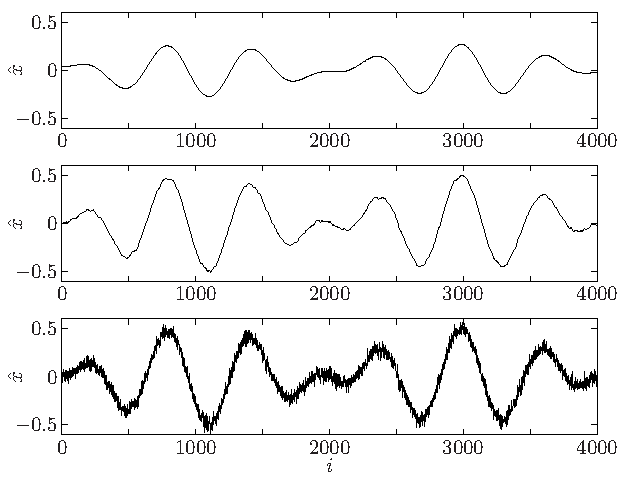
\includegraphics[width=.82\textwidth]{ch06-10.pdf}
\caption*{图6.10\quad 三个平滑或重构后的信号 $\widehat x$。上图对应 $\norm{\widehat x-x_{\rm cor}}_2=8$，中图对应 $\norm{\widehat x-x_{\rm cor}}_2=3$，下图对应 $\norm{\widehat x-x_{\rm cor}}_2=1$。}
\end{figure}
与二次平滑程度指标 $\phi_{\rm quad}$ 类似，全变差函数对变化迅速的 $\widehat x$ 赋予较大的值。不过，全变差指标对较大的 $|x_{i+1}-x_i|$ 赋予的惩罚相对较小。

\subsubsection*{全变差重构的例子}
图6.11给出信号 $x\in\R^{2000}$（上图）以及受噪声污染的信号 $x_{\rm cor}$。信号大体平滑，但有几处快速变化或跳变；噪声则变化迅速。

先采用二次平滑。图6.12给出 $\norm{D\widehat x}_2$ 与 $\norm{\widehat x-x_{\rm cor}}_2$ 最优权衡曲线上的三个平滑信号。在前两个信号中，原信号的快速变化也被平滑了。在第三个信号中，陡峭边缘保留得较好，但仍有大量噪声。

再来看全变差重构。图6.13是 $\norm{D\widehat x}_1$ 与 $\norm{\widehat x-x_{\rm cor}}_2$ 的最优权衡曲线。图6.14给出该曲线上对应 $\norm{D\widehat x}_1=5$（上）、$8$（中）和 $10$（下）的重构信号。可以看到，与二次平滑不同，全变差重构保留了信号中的突变。

% Source PDF page 329 (printed p. 315)
\begin{figure}[htbp]\centering
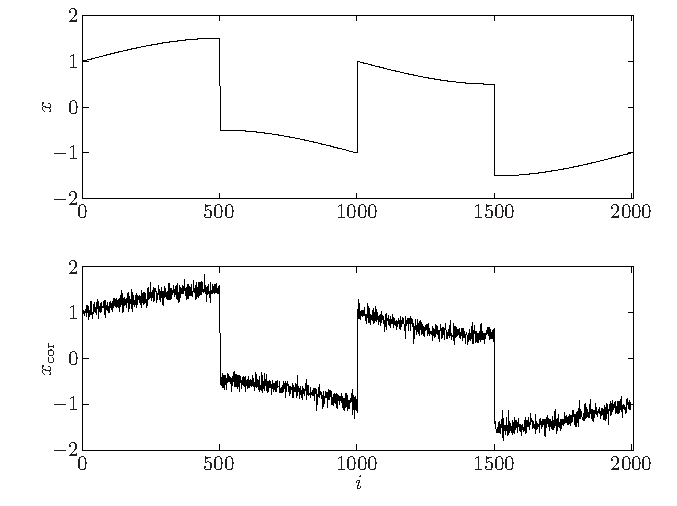
\includegraphics[width=.85\textwidth]{ch06-11.pdf}
\caption*{图6.11\quad 信号 $x\in\R^{2000}$ 及受污染信号 $x_{\rm cor}\in\R^{2000}$。噪声变化迅速，而信号大体平滑，只有几处快速变化。}
\end{figure}

% Source PDF page 330 (printed p. 316)
\begin{figure}[htbp]\centering
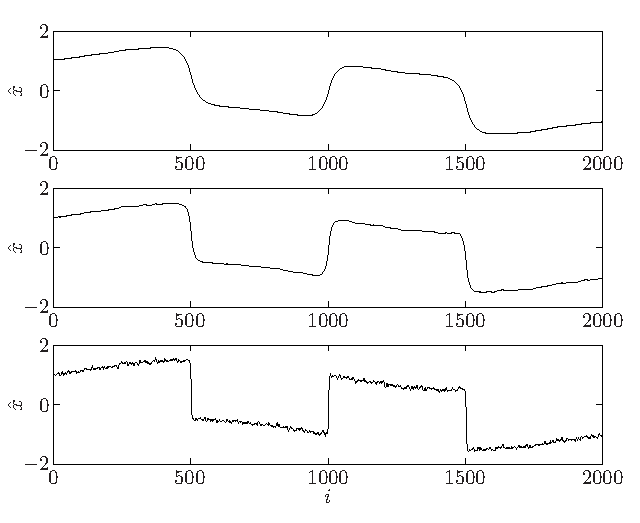
\includegraphics[width=.82\textwidth]{ch06-12.pdf}
\caption*{图6.12\quad 三个经二次平滑的信号 $\widehat x$。上图对应 $\norm{\widehat x-x_{\rm cor}}_2=10$，中图对应 $7$，下图对应 $4$。上图大幅降低噪声，但也过度平滑了信号中的快速变化。最下方的平滑信号降噪不足，同时仍平滑了原信号的快速变化。中间信号给出了最好的折中，但仍会平滑快速变化。}
\end{figure}
\begin{figure}[htbp]\centering
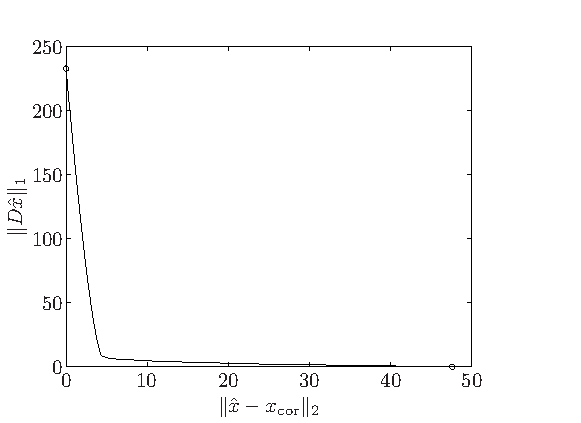
\includegraphics[width=.68\textwidth]{ch06-13.pdf}
\caption*{图6.13\quad $\norm{D\widehat x}_1$ 与 $\norm{\widehat x-x_{\rm cor}}_2$ 之间的最优权衡曲线。}
\end{figure}

% Source PDF page 331 (printed p. 317)
\begin{figure}[htbp]\centering
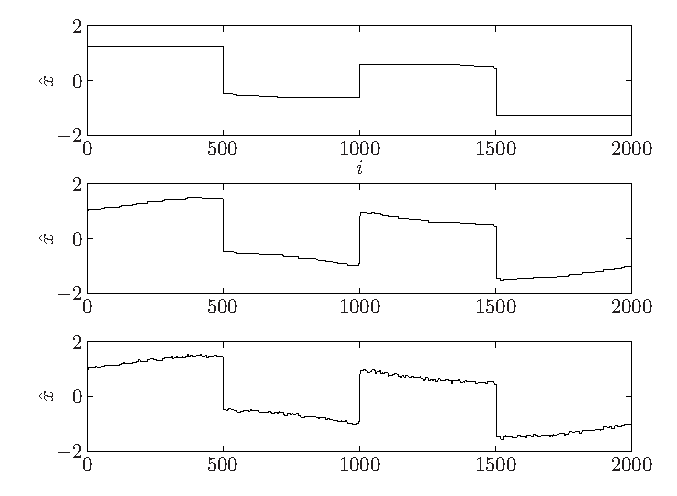
\includegraphics[width=.85\textwidth]{ch06-14.pdf}
\caption*{图6.14\quad 采用全变差重构得到的三个信号 $\widehat x$。上图对应 $\norm{D\widehat x}_1=5$，中图对应 $8$，下图对应 $10$。下图的噪声消除稍显不足，上图则消除了信号中一些缓慢变化的部分。注意，与二次平滑不同，全变差重构保留了信号中的突变。}
\end{figure}

% Source PDF page 332 (printed p. 318)
\section{稳健逼近}
\subsection{随机稳健逼近}
考虑基本目标为 $\norm{Ax-b}$ 的逼近问题，同时希望考虑数据矩阵 $A$ 的不确定性或可能变化。（同样的想法可以扩展到 $A$、$b$ 都不确定的情形。）本节用统计模型描述 $A$ 的变化。

假设 $A$ 是取值于 $\R^{m\times n}$、均值为 $\overline A$ 的随机变量，因此可以写为
\[A=\overline A+U,\]
其中 $U$ 是零均值随机矩阵。常矩阵 $\overline A$ 给出 $A$ 的平均值，$U$ 描述它的统计变化。

自然可以用 $\norm{Ax-b}$ 的期望作为目标：
\begin{equation}\text{最小化}\quad\E\norm{Ax-b}.\tag{6.13}\end{equation}
称其为\emph{随机稳健逼近问题}。它总是一个凸优化问题，但通常难以处理，因为在大多数情况下，计算目标或其导数都非常困难。

当 $A$ 只取有限个值时，随机稳健逼近问题 (6.13) 可以求解。这是一个简单情形，即
\[\Prob(A=A_i)=p_i,\qquad i=1,\ldots,k,\]
其中 $A_i\in\R^{m\times n}$、$\one^\T p=1$、$p\succeq0$。此时问题 (6.13) 为
\[\text{最小化}\quad p_1\norm{A_1x-b}+\cdots+p_k\norm{A_kx-b},\]
通常称为\emph{范数和问题}。它可表示为
\[\begin{array}{ll}\text{最小化}&p^\T t\\\text{约束条件}&\norm{A_ix-b}\le t_i,\quad i=1,\ldots,k,\end{array}\]
变量为 $x\in\R^n$、$t\in\R^k$。如果范数是欧几里得范数，这个范数和问题就是 SOCP。如果采用 $\ell_1$ 或 $\ell_\infty$ 范数，则可写为 LP，见习题6.8。

随机稳健逼近问题 (6.13) 的一些变体是可处理的。例如，考虑随机稳健最小二乘问题
\[\text{最小化}\quad\E\norm{Ax-b}_2^2,\]
其中范数为欧几里得范数。其目标可表示为
\[\begin{aligned}
\E\norm{Ax-b}_2^2
&=\E(\overline Ax-b+Ux)^\T(\overline Ax-b+Ux)\\
&=(\overline Ax-b)^\T(\overline Ax-b)+\E x^\T U^\T Ux\\
&=\norm{\overline Ax-b}_2^2+x^\T Px,
\end{aligned}\]
其中 $P=\E U^\T U$。

% Source PDF page 333 (printed p. 319)
因此，该随机稳健逼近问题具有正则化最小二乘问题的形式
\[\text{最小化}\quad\norm{\overline Ax-b}_2^2+\norm{P^{1/2}x}_2^2,\]
其解为
\[x=(\overline A^\T\overline A+P)^{-1}\overline A^\T b.\]
这完全符合直觉：矩阵 $A$ 有变化时，$x$ 越大，向量 $Ax$ 的变化也越大；而 Jensen 不等式告诉我们，$Ax$ 的变化会使 $\norm{Ax-b}_2$ 的平均值增大。因此，需要在使 $\overline Ax-b$ 较小与希望 $x$ 较小（以使 $Ax$ 的变化较小）之间作权衡，这正是正则化的核心想法。

这一观察也为 Tikhonov 正则化最小二乘问题 (6.10) 提供了另一种解释：它是考虑矩阵 $A$ 可能变化的稳健最小二乘问题。Tikhonov 正则化最小二乘问题 (6.10) 的解，使 $\E\norm{(A+U)x-b}^2$ 最小，其中 $U_{ij}$ 是零均值、不相关、方差为 $\delta/m$ 的随机变量（这里 $A$ 是确定性的）。

\subsection{最坏情形稳健逼近}
也可以用基于集合的最坏情形方法描述矩阵 $A$ 的变化。用 $A$ 的可能取值集合来描述不确定性：
\[A\in\mathcal A\subseteq\R^{m\times n},\]
假设该集合非空且有界。对于候选近似解 $x\in\R^n$，定义其对应的最坏情形误差
\[e_{\rm wc}(x)=\sup\{\norm{Ax-b}\mid A\in\mathcal A\},\]
它总是 $x$ 的凸函数。\emph{最坏情形稳健逼近问题}就是最小化最坏情形误差：
\begin{equation}
\text{最小化}\quad e_{\rm wc}(x)=\sup\{\norm{Ax-b}\mid A\in\mathcal A\},\tag{6.14}
\end{equation}
变量为 $x$，问题数据为 $b$ 和集合 $\mathcal A$。当 $\mathcal A=\{A\}$ 仅含一个元素时，稳健逼近问题 (6.14) 化为基本范数逼近问题 (6.1)。稳健逼近问题总是凸优化问题，但是否可处理，取决于所用范数以及不确定集 $\mathcal A$ 的描述方式。

\begin{origexample}{6.5}
\emph{随机稳健逼近与最坏情形稳健逼近的比较。}为说明稳健逼近问题的随机表述与最坏情形表述之间的区别，考虑最小二乘问题
\[\text{最小化}\quad\norm{A(u)x-b}_2^2,\]
其中 $u\in\R$ 是不确定参数，$A(u)=A_0+uA_1$。考虑一个具体实例，$A(u)\in\R^{20\times10}$、$\norm{A_0}=10$、$\norm{A_1}=1$，且 $u$ 位于区间 $[-1,1]$。（因此粗略地说，矩阵 $A$ 的变化幅度约为 $\pm10\%$。）

% Source PDF page 334 (printed p. 320)
\begin{figure}[htbp]\centering
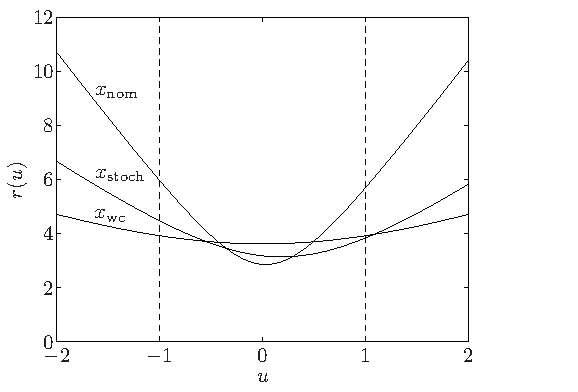
\includegraphics[width=.65\textwidth]{ch06-15.pdf}
\caption*{图6.15\quad 对三个近似解 $x$，绘出残差 $r(u)=\norm{A(u)x-b}_2$ 随不确定参数 $u$ 的变化：(1) 标称最小二乘解 $x_{\rm nom}$；(2) 随机稳健逼近问题的解 $x_{\rm stoch}$，假定 $u$ 在 $[-1,1]$ 上均匀分布；(3) 最坏情形稳健逼近问题的解 $x_{\rm wc}$，假定 $u\in[-1,1]$。标称解在 $u=0$ 时残差最小，但当 $u$ 接近 $-1$ 或 $1$ 时，残差大得多。最坏情形解在 $u=0$ 时残差较大，但当 $u$ 在 $[-1,1]$ 中变化时，残差增幅很小。}
\end{figure}
求三个近似解：
\begin{itemize}
\item \emph{标称最优解。}假定 $A(u)$ 取其标称值 $A_0$，求得最优解 $x_{\rm nom}$。
\item \emph{随机稳健逼近。}假定参数 $u$ 在 $[-1,1]$ 上均匀分布，求使 $\E\norm{A(u)x-b}_2^2$ 最小的 $x_{\rm stoch}$。
\item \emph{最坏情形稳健逼近。}求 $x_{\rm wc}$，使
\[\begin{split}\sup_{-1\le u\le1}\norm{A(u)x-b}_2
=\max\{&\norm{(A_0-A_1)x-b}_2,\\&\norm{(A_0+A_1)x-b}_2\}\end{split}\]
最小。
\end{itemize}
对这三个 $x$，图6.15分别绘出残差 $r(u)=\norm{A(u)x-b}_2$ 随不确定参数 $u$ 的变化。这些图说明，近似解可能对参数 $u$ 的变化十分敏感。标称解在 $u=0$ 时残差最小，但对参数变化颇为敏感：当 $u$ 偏离零并接近 $-1$ 或 $1$ 时，残差大得多。最坏情形解在 $u=0$ 时残差较大，但当 $u$ 在 $[-1,1]$ 内变化时，残差增幅很小。随机稳健近似解介于二者之间。
\end{origexample}

% Source PDF page 335 (printed p. 321)
稳健逼近问题 (6.14) 出现在许多场合和应用中。在估计问题中，集合 $\mathcal A$ 描述待估向量与测量向量之间线性关系的不确定性。模型 $y=Ax+v$ 中的噪声项 $v$ 有时称为\emph{加性噪声}或\emph{加性误差}，因为它加在“理想”测量 $Ax$ 上。相对地，$A$ 的变化称为\emph{乘性误差}，因为它与变量 $x$ 相乘。

在最优设计中，这种变化可以表示连接设计变量 $x$ 与结果向量 $Ax$ 的线性方程的不确定性，例如来自制造过程的不确定性。此时，稳健逼近问题 (6.14) 就解释为稳健设计问题：寻找设计变量 $x$，使对所有可能的 $A$ 而言，$Ax$ 与 $b$ 之间可能出现的最大偏差最小。

\subsubsection*{有限集合}
此时 $\mathcal A=\{A_1,\ldots,A_k\}$，稳健逼近问题为
\[\text{最小化}\quad\max_{i=1,\ldots,k}\norm{A_ix-b}.\]
它等价于采用多面体集合 $\mathcal A=\conv\{A_1,\ldots,A_k\}$ 的稳健逼近问题：
\[\text{最小化}\quad\sup\{\norm{Ax-b}\mid A\in\conv\{A_1,\ldots,A_k\}\}.\]
问题可以写成上图形式
\[\begin{array}{ll}\text{最小化}&t\\\text{约束条件}&\norm{A_ix-b}\le t,\quad i=1,\ldots,k.\end{array}\]
根据所用范数的不同，可以有多种求解方法。若采用欧几里得范数，它就是 SOCP；若采用 $\ell_1$ 或 $\ell_\infty$ 范数，则可以写成 LP。

\subsubsection*{范数有界误差}
这里不确定集 $\mathcal A$ 是一个范数球：$\mathcal A=\{\overline A+U\mid\norm U\le a\}$，其中 $\norm{\cdot}$ 是 $\R^{m\times n}$ 上的范数。于是
\[e_{\rm wc}(x)=\sup\{\norm{\overline Ax-b+Ux}\mid\norm U\le a\}.\]
需要仔细理解该式：第一个范数定义在 $\R^m$ 上，用于衡量残差大小；第二个范数定义在 $\R^{m\times n}$ 上，用于定义范数球 $\mathcal A$。

在若干情形下，$e_{\rm wc}(x)$ 的这一表达式可以简化。例如，在 $\R^n$ 上采用欧几里得范数，在 $\R^{m\times n}$ 上采用相应的诱导范数，即最大奇异值。如果 $\overline Ax-b\ne0$ 且 $x\ne0$，那么 $e_{\rm wc}(x)$ 中的上确界在 $U=auv^\T$ 处取得，其中
\[u=\frac{\overline Ax-b}{\norm{\overline Ax-b}_2},\qquad v=\frac x{\norm x_2},\]
从而最坏情形误差为
\[e_{\rm wc}(x)=\norm{\overline Ax-b}_2+a\norm x_2.\]

% Source PDF page 336 (printed p. 322)
（容易验证，$x$ 或 $\overline Ax-b$ 为零时，这一表达式同样成立。）稳健逼近问题 (6.14) 因此变成
\[\text{最小化}\quad\norm{\overline Ax-b}_2+a\norm x_2,\]
这是一个正则化范数问题，可以写成 SOCP
\[\begin{array}{ll}\text{最小化}&t_1+at_2\\\text{约束条件}&\norm{\overline Ax-b}_2\le t_1,\quad\norm x_2\le t_2.\end{array}\]
对某个正则化参数 $\delta$，该问题的解与正则化最小二乘问题
\[\text{最小化}\quad\norm{\overline Ax-b}_2^2+\delta\norm x_2^2\]
的解相同，因此又得到了将正则化最小二乘问题解释为最坏情形稳健逼近问题的一种方式。

\subsubsection*{不确定性椭球}
也可以为 $A$ 的每一行给出一个可能取值的椭球，以描述 $A$ 的变化：
\[\mathcal A=\{[a_1\ \cdots\ a_m]^\T\mid a_i\in\mathcal E_i,\ i=1,\ldots,m\},\]
其中
\[\mathcal E_i=\{\overline a_i+P_i u\mid\norm u_2\le1\}.\]
矩阵 $P_i\in\R^{n\times n}$ 描述 $a_i$ 的变化。允许 $P_i$ 具有非平凡零空间，以刻画 $a_i$ 的变化局限于某个子空间的情形。极端情况下，若 $a_i$ 没有不确定性，就取 $P_i=0$。

在这种椭球不确定性描述下，每个残差幅度的最坏值有显式表达式：
\[\begin{aligned}
\sup_{a_i\in\mathcal E_i}|a_i^\T x-b_i|
&=\sup\{|\overline a_i^\T x-b_i+(P_iu)^\T x|\mid\norm u_2\le1\}\\
&=|\overline a_i^\T x-b_i|+\norm{P_i^\T x}_2.
\end{aligned}\]
利用这一结果，可以求解若干稳健逼近问题。例如，稳健 $\ell_2$ 范数逼近问题
\[\text{最小化}\quad e_{\rm wc}(x)=\sup\{\norm{Ax-b}_2\mid a_i\in\mathcal E_i,\ i=1,\ldots,m\}\]
可以按以下方式化为 SOCP。最坏情形误差的显式表达式为
\[\begin{aligned}
e_{\rm wc}(x)&=\left(\sum_{i=1}^m\sup_{a_i\in\mathcal E_i}|a_i^\T x-b_i|^2\right)^{1/2}\\
&=\left(\sum_{i=1}^m\bigl(|\overline a_i^\T x-b_i|+\norm{P_i^\T x}_2\bigr)^2\right)^{1/2}.
\end{aligned}\]
为了最小化 $e_{\rm wc}(x)$，可以求解
\[\begin{array}{ll}\text{最小化}&\norm t_2\\\text{约束条件}&|\overline a_i^\T x-b_i|+\norm{P_i^\T x}_2\le t_i,\quad i=1,\ldots,m,\end{array}\]
其中引入了新变量 $t_1,\ldots,t_m$。

% Source PDF page 337 (printed p. 323)
该问题可以表述为
\[\begin{array}{ll}\text{最小化}&\norm t_2\\\text{约束条件}&\overline a_i^\T x-b_i+\norm{P_i^\T x}_2\le t_i,\quad i=1,\ldots,m,\\&-\overline a_i^\T x+b_i+\norm{P_i^\T x}_2\le t_i,\quad i=1,\ldots,m,\end{array}\]
写成上图形式后就成为 SOCP。

\subsubsection*{具有线性结构的范数有界误差}
作为范数有界描述 $\mathcal A=\{\overline A+U\mid\norm U\le a\}$ 的推广，可以将 $\mathcal A$ 定义为一个范数球在仿射变换下的像：
\[\mathcal A=\{\overline A+u_1A_1+u_2A_2+\cdots+u_pA_p\mid\norm u\le1\},\]
其中 $\norm{\cdot}$ 是 $\R^p$ 上的范数，$p+1$ 个矩阵 $\overline A,A_1,\ldots,A_p\in\R^{m\times n}$ 已知。最坏情形误差可写为
\[\begin{aligned}
e_{\rm wc}(x)&=\sup_{\norm u\le1}\norm{(\overline A+u_1A_1+\cdots+u_pA_p)x-b}\\
&=\sup_{\norm u\le1}\norm{P(x)u+q(x)},
\end{aligned}\]
其中 $P$ 和 $q$ 定义为
\[P(x)=[A_1x\ A_2x\ \cdots\ A_px]\in\R^{m\times p},\qquad q(x)=\overline Ax-b\in\R^m.\]
先考虑稳健 Chebyshev 逼近问题
\[\text{最小化}\quad e_{\rm wc}(x)=\sup_{\norm u_\infty\le1}\norm{(\overline A+u_1A_1+\cdots+u_pA_p)x-b}_\infty.\]
此时可以导出最坏情形误差的显式表达式。令 $p_i(x)^\T$ 为 $P(x)$ 的第 $i$ 行，有
\[\begin{aligned}
e_{\rm wc}(x)&=\sup_{\norm u_\infty\le1}\norm{P(x)u+q(x)}_\infty\\
&=\max_{i=1,\ldots,m}\sup_{\norm u_\infty\le1}|p_i(x)^\T u+q_i(x)|\\
&=\max_{i=1,\ldots,m}\bigl(\norm{p_i(x)}_1+|q_i(x)|\bigr).
\end{aligned}\]
因此，稳健 Chebyshev 逼近问题可以写为 LP
\[\begin{array}{ll}\text{最小化}&t\\\text{约束条件}&-y_0\preceq\overline Ax-b\preceq y_0,\\&-y_k\preceq A_kx\preceq y_k,\quad k=1,\ldots,p,\\&y_0+\displaystyle\sum_{k=1}^p y_k\preceq t\one,\end{array}\]
变量为 $x\in\R^n$、$y_k\in\R^m$、$t\in\R$。

再考虑稳健最小二乘问题
\[\text{最小化}\quad e_{\rm wc}(x)=\sup_{\norm u_2\le1}\norm{(\overline A+u_1A_1+\cdots+u_pA_p)x-b}_2.\]

% Source PDF page 338 (printed p. 324)
这里使用拉格朗日对偶来计算 $e_{\rm wc}$。最坏情形误差 $e_{\rm wc}(x)$ 是如下非凸二次优化问题最优值的平方根：
\[\begin{array}{ll}\text{最大化}&\norm{P(x)u+q(x)}_2^2\\\text{约束条件}&u^\T u\le1,\end{array}\]
变量为 $u$。这个问题的拉格朗日对偶可以写成 SDP
\begin{equation}
\begin{array}{ll}\text{最小化}&t+\lambda\\\text{约束条件}&\begin{bmatrix}I&P(x)&q(x)\\P(x)^\T&\lambda I&0\\q(x)^\T&0&t\end{bmatrix}\succeq0,\end{array}\tag{6.15}
\end{equation}
变量为 $t,\lambda\in\R$。而且，正如第5.2节与第B.1节提到（并在第B.4节证明）的，这一对原问题与对偶问题满足强对偶。换言之，固定 $x$ 后，通过求解以 $t$、$\lambda$ 为变量的 SDP (6.15)，就能计算 $e_{\rm wc}(x)^2$。联合优化 $t$、$\lambda$ 和 $x$，等价于最小化 $e_{\rm wc}(x)^2$。因此，稳健最小二乘问题等价于以 $x$、$\lambda$、$t$ 为变量的 SDP (6.15)。

\begin{origexample}{6.6}
\emph{最坏情形稳健解、Tikhonov 正则化解与标称最小二乘解的比较。}考虑稳健逼近问题的一个实例：
\begin{equation}
\text{最小化}\quad\sup_{\norm u_2\le1}\norm{(\overline A+u_1A_1+u_2A_2)x-b}_2,\tag{6.16}
\end{equation}
维数为 $m=50$、$n=20$。矩阵 $\overline A$ 的范数为 $10$，矩阵 $A_1$、$A_2$ 的范数均为 $1$，因此粗略地说，矩阵 $A$ 的变化约为 $10\%$。不确定参数 $u_1$、$u_2$ 位于 $\R^2$ 的单位圆盘内。

计算稳健最小二乘问题 (6.16) 的最优解 $x_{\rm rls}$，以及标称最小二乘问题的解 $x_{\rm ls}$（即假定 $u=0$），还计算 $\delta=1$ 的 Tikhonov 正则化解 $x_{\rm tik}$。

为说明各个近似解对参数 $u$ 的敏感性，生成 $10^5$ 个在单位圆盘内均匀分布的参数向量，并对每个参数值计算残差
\[\norm{(A_0+u_1A_1+u_2A_2)x-b}_2.\]
残差分布见图6.16。

可以作出几点观察。首先，标称最小二乘解的残差分布很宽，从约 $0.52$ 的最小值到约 $4.9$ 的最大值。特别地，最小二乘解对参数变化非常敏感。相反，当不确定参数在单位圆盘内变化时，稳健最小二乘解和 Tikhonov 正则化解的残差变化小得多。例如，稳健最小二乘解在单位圆盘内所有参数下的残差都介于 $2.0$ 与 $2.6$ 之间。
\end{origexample}

\section{函数拟合与插值}
函数拟合问题要从一个有限维函数子空间中选择一个函数，使其最好地满足给定的数据或要求。为简便起见，只考虑实值函数；这些想法也容易扩展到向量值函数。

% Source PDF page 339 (printed p. 325)
\begin{figure}[htbp]\centering
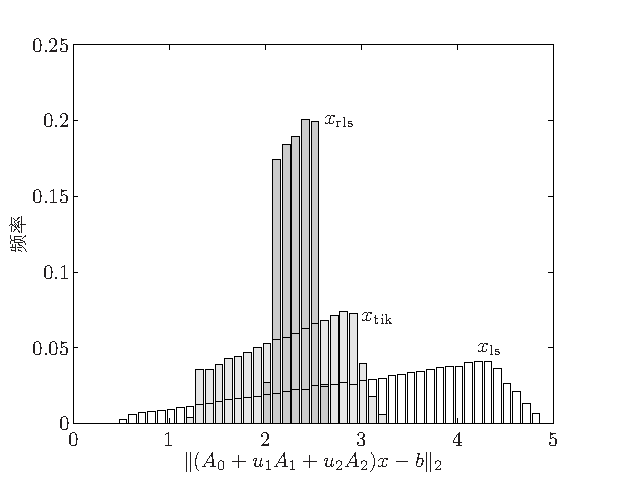
\includegraphics[width=.72\textwidth]{ch06-16.pdf}
\caption*{图6.16\quad 最小二乘问题 (6.16) 的三个解所对应的残差分布：$x_{\rm ls}$ 是假定 $u=0$ 的最小二乘解；$x_{\rm tik}$ 是 $\delta=1$ 的 Tikhonov 正则化解；$x_{\rm rls}$ 是稳健最小二乘解。这些直方图通过从 $\R^2$ 单位圆盘上的均匀分布中生成 $10^5$ 个不确定参数向量 $u$ 得到，分箱宽度为 $0.1$。}
\end{figure}

% Source PDF page 340 (printed p. 326)
\subsection{函数族}
考虑函数族 $f_1,\ldots,f_n:\R^k\to\R$，它们具有共同定义域 $\dom f_i=\mathcal D$。对每个 $x\in\R^n$，关联函数 $f:\R^k\to\R$，定义为
\begin{equation}f(u)=x_1f_1(u)+\cdots+x_nf_n(u),\tag{6.17}\end{equation}
且 $\dom f=\mathcal D$。即使函数不线性无关，函数族 $\{f_1,\ldots,f_n\}$ 有时也称为拟合问题的\emph{基函数}集。将函数子空间参数化的向量 $x\in\R^n$ 是优化变量，有时称为\emph{系数向量}。这些基函数生成 $\mathcal D$ 上的函数子空间 $\mathcal F$。

在许多应用中，会利用先验知识或经验专门选择基函数，以便用有限维函数子空间合理地描述所关心的函数。另一些情况下，则采用更通用的函数族。下面介绍其中几种。

\subsubsection*{多项式}
$\R$ 上的一个常用函数子空间，是次数小于 $n$ 的多项式空间。最简单的基由幂函数构成，即 $f_i(t)=t^{i-1}$，$i=1,\ldots,n$。许多应用中，会用另一组基描述同一子空间；例如采用次数小于 $n$ 的一组多项式 $f_1,\ldots,f_n$，使它们关于某个正函数（或测度）$\phi:\R^n\to\R_+$ 正交归一，即
\[\int f_i(t)f_j(t)\phi(t)\,dt=\begin{cases}1,&i=j,\\0,&i\ne j.\end{cases}\]
另一组常用多项式基，是与互异点 $t_1,\ldots,t_n$ 对应的 Lagrange 基 $f_1,\ldots,f_n$，满足
\[f_i(t_j)=\begin{cases}1,&i=j,\\0,&i\ne j.\end{cases}\]
也可以考虑 $\R^k$ 上的多项式，限制其最大总次数，或每个变量的最高次数。

一个相关例子是次数小于 $n$ 的三角多项式，其基为
\[\sin kt,\quad k=1,\ldots,n-1,\qquad\cos kt,\quad k=0,\ldots,n-1.\]

\subsubsection*{分段线性函数}
先对定义域 $\mathcal D$ 作三角剖分，其含义如下。给定一组网格点 $g_1,\ldots,g_n\in\R^k$，并将 $\mathcal D$ 划分为一组单纯形：
\[\mathcal D=S_1\cup\cdots\cup S_m,\qquad\operatorname{int}(S_i\cap S_j)=\varnothing\quad(i\ne j).\]
每个单纯形是 $k+1$ 个网格点的凸包，而且要求：一个网格点若属于某个单纯形，就必须是它的顶点。

% Source PDF page 341 (printed p. 327)
\begin{figure}[htbp]\centering
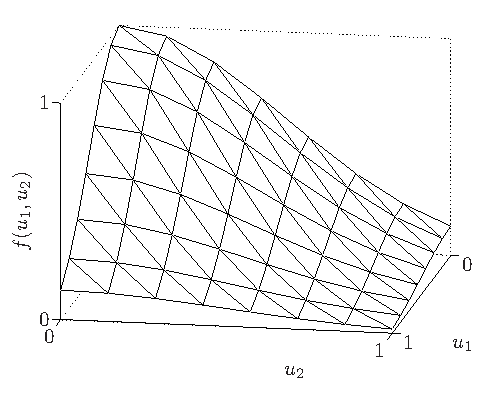
\includegraphics[width=.64\textwidth]{ch06-17.pdf}
\caption*{图6.17\quad 单位正方形上的二元分段线性函数。三角剖分由单位正方形内的64个均匀网格点和98个单纯形构成。}
\end{figure}
给定三角剖分后，可以先给网格点赋函数值 $f(g_i)=x_i$，再在每个单纯形上作仿射延拓，构造分段线性函数（更准确地说，分段仿射函数）$f$。函数 $f$ 可写为式 (6.17)，其中基函数 $f_i$ 在每个单纯形上仿射，并由下述条件定义：
\[f_i(g_j)=\begin{cases}1,&i=j,\\0,&i\ne j.\end{cases}\]
按这种构造得到的函数是连续的。

图6.17给出了 $k=2$ 的一个例子。

\subsubsection*{分段多项式与样条}
三角剖分定义域上的分段仿射函数这一想法，容易推广到分段多项式和其他函数。

分段多项式在三角剖分的每个单纯形上定义为某个最高次数以下的多项式，并且是连续的，即相邻单纯形上的多项式在公共边界处取值一致。进一步要求分段多项式直到某一阶的导数连续，就可以定义各种样条函数。图6.18是三次样条的例子，即 $\R$ 上一阶、二阶导数连续的三次分段多项式。

% Source PDF page 342 (printed p. 328)
\begin{figure}[htbp]\centering
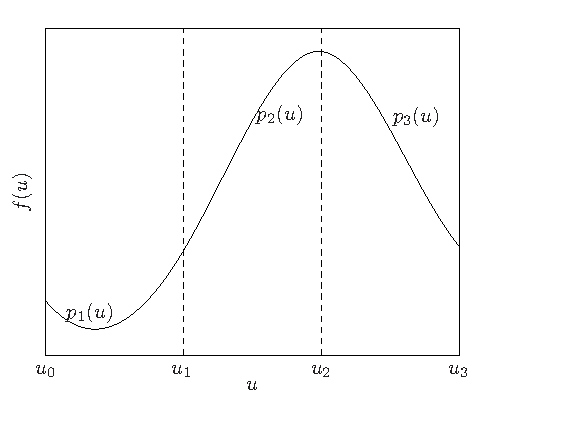
\includegraphics[width=.65\textwidth]{ch06-18.pdf}
\caption*{图6.18\quad 三次样条。三次样条是具有连续一阶、二阶导数的分段多项式。本例中，三次样条 $f$ 由三个三次多项式构成：$p_1$ 定义在 $[u_0,u_1]$，$p_2$ 定义在 $[u_1,u_2]$，$p_3$ 定义在 $[u_2,u_3]$。相邻多项式在边界点 $u_1$、$u_2$ 处函数值相等，一阶、二阶导数也相等。本例中函数族的维数为 $n=6$，因为有12个多项式系数（每个三次多项式4个），以及6个等式约束（$u_1$、$u_2$ 处各3个）。}
\end{figure}

% Source PDF page 343 (printed p. 329)
\subsection{约束}
本节介绍可以施加在函数 $f$ 上、从而施加在变量 $x\in\R^n$ 上的一些约束。

\subsubsection*{函数值插值与不等式}
令 $v$ 为 $\mathcal D$ 中的一点。$f$ 在 $v$ 的值
\[f(v)=\sum_{i=1}^n x_i f_i(v)\]
是 $x$ 的线性函数。因此，要求函数 $f$ 在指定点 $v_j\in\mathcal D$ 处取指定值 $z_j\in\R$ 的插值条件
\[f(v_j)=z_j,\qquad j=1,\ldots,m,\]
构成关于 $x$ 的一组线性等式。更一般地，对给定点函数值的不等式要求，如 $l\le f(v)\le u$，也是关于变量 $x$ 的线性不等式。还有许多涉及有限点集 $v_1,\ldots,v_N$ 上函数值的有意义的凸约束。例如，Lipschitz 约束
\[|f(v_j)-f(v_k)|\le L\norm{v_j-v_k},\qquad j,k=1,\ldots,m,\]
构成关于 $x$ 的一组线性不等式。

也可以对无穷多个点上的函数值施加不等式。例如，考虑非负约束
\[f(u)\ge0\quad\text{对所有 }u\in\mathcal D.\]
这是关于 $x$ 的凸约束，因为它是无穷多个半空间的交；但除非利用函数特殊结构的某些情形，否则未必得到可处理的问题。一个简单例子是分段线性函数：如果网格点处的函数值非负，函数就处处非负，因此只需一组简单的有限线性不等式。

再看一个不那么简单的例子。考虑 $\R$ 上最高次数为偶数 $2k$ 的多项式，即 $n=2k+1$，并令 $\mathcal D=\R$。如第65页习题2.37所示，非负约束
\[p(u)=x_1+x_2u+\cdots+x_{2k+1}u^{2k}\ge0\quad\text{对所有 }u\in\R\]
等价于
\[x_i=\sum_{m+n=i+1}Y_{mn},\quad i=1,\ldots,2k+1,\qquad Y\succeq0,\]
其中 $Y\in\mathbf S^{k+1}$ 是辅助变量。

% Source PDF page 344 (printed p. 330)
\subsubsection*{导数约束}
假设基函数 $f_i$ 在点 $v\in\mathcal D$ 可微。梯度
\[\nabla f(v)=\sum_{i=1}^n x_i\nabla f_i(v)\]
是 $x$ 的线性函数，因此对 $f$ 在 $v$ 处导数的插值条件，可化为关于 $x$ 的线性等式约束。要求 $v$ 处梯度的范数不超过给定上限，
\[\norm{\nabla f(v)}=\left\|\sum_{i=1}^n x_i\nabla f_i(v)\right\|\le M,\]
是关于 $x$ 的凸约束。同样的想法也适用于高阶导数。例如，如果 $f$ 在 $v$ 二阶可微，则要求
\[lI\preceq\nabla^2f(v)\preceq uI\]
是关于 $x$ 的线性矩阵不等式，因此为凸约束。

也可以对无穷多个点处的导数施加约束。例如，要求 $f$ 单调：
\[f(u)\ge f(v)\quad\text{对所有 }u,v\in\mathcal D,\ u\succeq v.\]
这是关于 $x$ 的凸约束，但除某些特殊情形外，未必得到可处理的问题。例如，当 $f$ 分段仿射时，单调性约束等价于每个单纯形内部有 $\nabla f(v)\succeq0$。由于梯度是网格点取值的线性函数，这就得到一组简单的有限线性不等式。

另一个例子是要求函数为凸函数，即满足
\[f((u+v)/2)\le(f(u)+f(v))/2\quad\text{对所有 }u,v\in\mathcal D\]
（$f$ 连续时，这足以保证凸性）。这是一个凸约束，在某些情况下具有可处理的表示。一个明显的例子是 $f$ 为二次函数，此时凸性约束等价于要求 $f$ 的二次部分非负，这就是一个 LMI。第6.5.5节将更详细地介绍另一个凸性约束产生可处理问题的例子。

\subsubsection*{积分约束}
函数子空间上的任意线性泛函 $L$ 都可表示为 $x$ 的线性函数，即 $L(f)=c^\T x$。在某点求 $f$ 或其导数的值，只是一个特例。另一个例子是线性泛函
\[L(f)=\int_{\mathcal D}\phi(u)f(u)\,du,\]

% Source PDF page 345 (printed p. 331)
其中 $\phi:\R^k\to\R$，它可表示为 $L(f)=c^\T x$，其中
\[c_i=\int_{\mathcal D}\phi(u)f_i(u)\,du.\]
因此，形如 $L(f)=a$ 的约束，是关于 $x$ 的线性等式约束。一个例子是矩约束
\[\int_{\mathcal D}t^mf(t)\,dt=a\]
（其中 $f:\R\to\R$）。

\subsection{拟合与插值问题}
\subsubsection*{最小范数函数拟合}
在拟合问题中，给定数据
\[(u_1,y_1),\quad\ldots,\quad(u_m,y_m),\]
其中 $u_i\in\mathcal D$、$y_i\in\R$，要寻找尽可能贴近这些数据的函数 $f\in\mathcal F$。例如，在最小二乘拟合中，考虑问题
\[\text{最小化}\quad\sum_{i=1}^m(f(u_i)-y_i)^2,\]
这是一个以 $x$ 为变量的简单最小二乘问题。可以加入多种约束，例如 $f$ 在各个点处必须满足的线性不等式、对 $f$ 导数的约束、单调性约束或矩约束。

\begin{origexample}{6.7}
\emph{多项式拟合。}给定数据 $u_1,\ldots,u_m\in\R$ 和 $v_1,\ldots,v_m\in\R$，希望用如下形式的多项式近似拟合数据：
\[p(u)=x_1+x_2u+\cdots+x_nu^{n-1}.\]
对每个 $x$，形成误差向量
\[e=(p(u_1)-v_1,\ldots,p(u_m)-v_m).\]
为了找出使误差范数最小的多项式，求解范数逼近问题
\[\text{最小化}\quad\norm e=\norm{Ax-v},\]
变量为 $x\in\R^n$，其中 $A_{ij}=u_i^{j-1}$，$i=1,\ldots,m$，$j=1,\ldots,n$。

图6.19给出 $m=40$ 个数据点、$n=6$（即最高次数为5的多项式）时采用 $\ell_2$ 和 $\ell_\infty$ 范数的例子。
\end{origexample}

% Source PDF page 346 (printed p. 332)
\begin{figure}[htbp]\centering
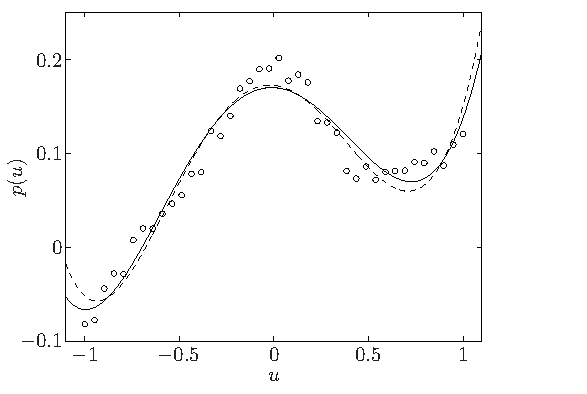
\includegraphics[width=.66\textwidth]{ch06-19.pdf}
\caption*{图6.19\quad 逼近图中以圆圈标出的40个数据点的两个5次多项式。实线多项式最小化误差的 $\ell_2$ 范数，虚线多项式最小化误差的 $\ell_\infty$ 范数。}
\end{figure}
\begin{figure}[htbp]\centering
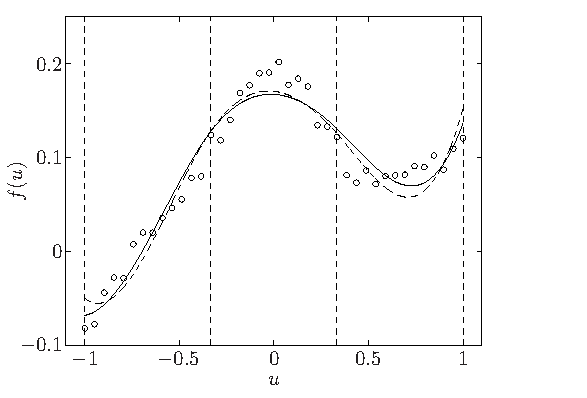
\includegraphics[width=.66\textwidth]{ch06-20.pdf}
\caption*{图6.20\quad 逼近图中以圆圈标出的40个数据点的两个三次样条；数据与图6.19相同。实线样条最小化误差的 $\ell_2$ 范数，虚线样条最小化误差的 $\ell_\infty$ 范数。与图6.19中的多项式逼近一样，拟合函数子空间的维数为6。}
\end{figure}

% Source PDF page 347 (printed p. 333)
\begin{origexample}{6.8}
\emph{样条拟合。}图6.20给出与例6.7相同的数据，以及用三次样条得到的两个最优拟合。将区间 $[-1,1]$ 等分为三个区间，考虑最高次数为3、一阶和二阶导数连续的分段多项式。这个函数子空间的维数为6，与例6.7中最高次数为5的多项式空间维数相同。
\end{origexample}

在最简单的函数拟合中，有 $m\gg n$，即数据点数远大于函数子空间维数。由于子空间中的所有函数都平滑，拟合会自动起到平滑作用。

\subsubsection*{最小范数插值}
在函数拟合的另一种变体中，数据点数少于函数子空间维数。最简单的情形，是要求选定函数满足插值条件
\[f(u_i)=y_i,\qquad i=1,\ldots,m,\]
这是关于 $x$ 的线性等式约束。在满足这些插值条件的函数中，可以寻找最平滑或最小的函数。这就得到最小范数问题。

在最一般的函数拟合问题中，可以在表示对背后函数的先验知识的各种凸约束下，优化某个目标，例如某种误差 $e$ 的度量。

\subsubsection*{插值、外推与求界}
在原数据集之外的点 $v$ 计算最优拟合函数 $\widehat f$，就得到对背后函数在 $v$ 处取值的猜测。如果 $v$ 位于给定数据点之间或附近，例如 $v\in\conv\{v_1,\ldots,v_m\}$，这称为\emph{插值}；否则称为\emph{外推}。

还可以在约束下最大化、最小化线性函数 $f(v)$，得到 $f(v)$ 可能取值的区间。可以利用函数拟合帮助识别错误数据或离群值。例如，采用 $\ell_1$ 范数拟合后，寻找误差较大的数据点。

\subsection{稀疏描述与基追踪}
在\emph{基追踪}中，基函数的数量非常大，目标是用少量基函数的线性组合很好地拟合给定数据。（此时函数族线性相关，有时称为\emph{过完备基}或\emph{字典}。）之所以称为基追踪，是因为要从给定过完备基中选出小得多的一组基来描述数据。

% Source PDF page 348 (printed p. 334)
因此，要寻找一个很好拟合数据的函数 $f\in\mathcal F$，使
\[f(u_i)\approx y_i,\qquad i=1,\ldots,m,\]
且系数向量 $x$ 稀疏，即 $\operatorname{card}(x)$ 小。此时称
\[f=x_1f_1+\cdots+x_nf_n=\sum_{i\in\mathcal B}x_if_i,\]
为数据的\emph{稀疏描述}，其中 $\mathcal B=\{i\mid x_i\ne0\}$ 是被选中基元素的指标集。从数学上看，基追踪与回归向量选择问题相同（见第6.4节），但优化问题的解释和规模不同。

稀疏描述与基追踪有许多用途，可以用于去噪、平滑，或对信号进行数据压缩以便高效传输或存储。在数据压缩中，发送方和接收方都知道字典或基元素。为了向接收方发送信号，发送方先寻找信号的稀疏表示，再只把非零系数以某种精度传给接收方。接收方用这些系数就能重构原信号的一个近似。

一种常用的基追踪方法，与第6.4节描述的回归向量选择方法相同，以 $\ell_1$ 范数正则化作为寻找稀疏描述的启发式方法。首先求解凸问题
\begin{equation}\text{最小化}\quad\sum_{i=1}^m(f(u_i)-y_i)^2+\gamma\norm x_1,\tag{6.18}\end{equation}
其中参数 $\gamma>0$ 用于在拟合数据的质量与系数向量的稀疏程度之间权衡。可以直接采用这个问题的解，也可以再进行精修：使用问题 (6.18) 的解所具有的稀疏模式，寻找最佳拟合。换言之，先求解 (6.18) 得到 $\widehat x$，然后令 $\mathcal B=\{i\mid\widehat x_i\ne0\}$，即非零系数对应的指标集。随后求解最小二乘问题
\[\text{最小化}\quad\sum_{i=1}^m(f(u_i)-y_i)^2,\]
变量为 $x_i$（$i\in\mathcal B$），并令 $i\notin\mathcal B$ 时 $x_i=0$。

基追踪与稀疏描述应用中的字典往往非常大，$n$ 可以在 $10^4$ 量级甚至更大。要高效求解 (6.18)，算法必须利用源于字典信号结构的问题结构。

\subsubsection*{用基追踪进行时频分析}
本节用一个简单例子说明基追踪与稀疏表示。考虑 $\R$ 上的函数或信号，关注范围为 $[0,1]$。把自变量理解为时间，因此用 $t$ 而非 $u$ 表示它。

先描述字典中的基函数。每个基函数都是一个高斯正弦脉冲，即 Gabor 函数，形式为
\[e^{-(t-\tau)^2/\sigma^2}\cos(\omega t+\phi),\]
其中 $\sigma>0$ 给出脉冲宽度，$\tau$ 是脉冲中心的时刻，$\omega\ge0$ 是频率，$\phi$ 是相位角。

% Source PDF page 349 (printed p. 335)
\begin{figure}[htbp]\centering
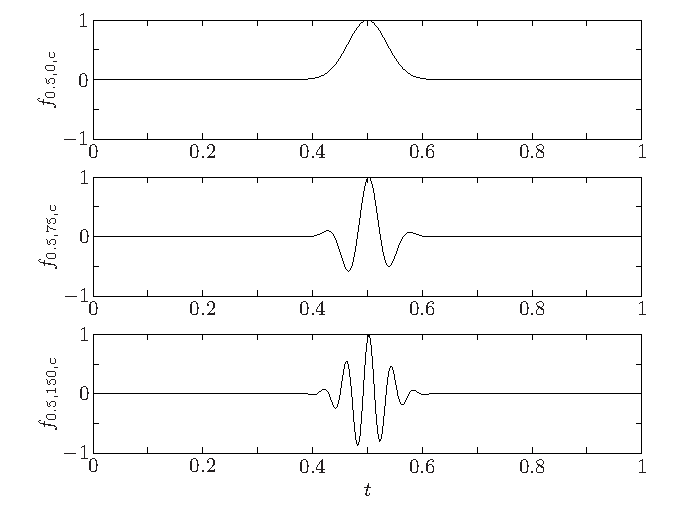
\includegraphics[width=.84\textwidth]{ch06-21.pdf}
\caption*{图6.21\quad 字典中的三个基元素，中心时刻均为 $\tau=0.5$，且均取余弦相位。上方信号频率为 $\omega=0$，中间为 $\omega=75$，下方为 $\omega=150$。}
\end{figure}
所有基函数宽度均为 $\sigma=0.05$。脉冲时刻与频率分别取
\[\tau=0.002k,\quad k=0,\ldots,500,\qquad\omega=5k,\quad k=0,\ldots,30.\]
对每个时刻 $\tau$，有一个零频率基元素（相位 $\phi=0$），以及其余30个频率各两个基元素（余弦和正弦，即相位 $\phi=0$、$\phi=\pi/2$），总共 $501\times61=30561$ 个基元素。自然可按时刻、频率与相位（余弦或正弦）对基元素编号，记作
\[\begin{aligned}
f_{\tau,\omega,c},&\quad\tau=0,0.002,\ldots,1,\quad\omega=0,5,\ldots,150,\\
f_{\tau,\omega,s},&\quad\tau=0,0.002,\ldots,1,\quad\omega=5,\ldots,150.
\end{aligned}\]
图6.21给出三个基函数，时刻均为 $\tau=0.5$。

采用这个字典的基追踪，可以看作对数据的时频分析。如果基元素 $f_{\tau,\omega,c}$ 或 $f_{\tau,\omega,s}$ 出现在信号的稀疏表示中，即对应系数非零，就可解释为：数据在时刻 $\tau$ 含有频率 $\omega$。

用基追踪寻找信号
\[y(t)=a(t)\sin\theta(t)\]
的稀疏近似，其中
\[a(t)=1+0.5\sin(11t),\qquad\theta(t)=30\sin(5t).\]

% Source PDF page 350 (printed p. 336)
\begin{figure}[htbp]\centering
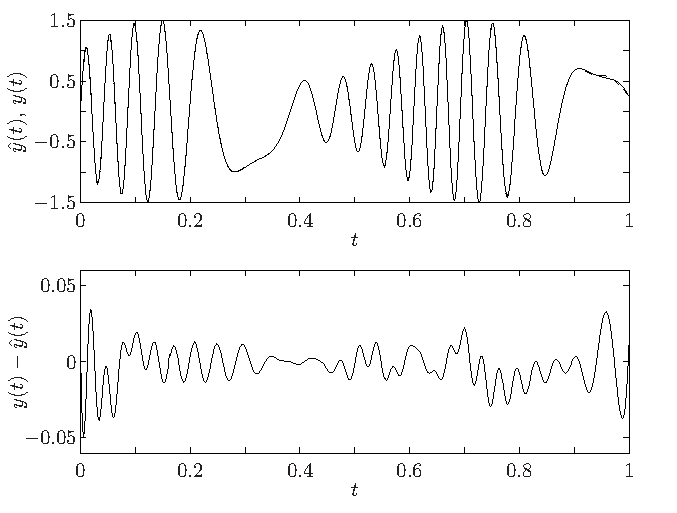
\includegraphics[width=.82\textwidth]{ch06-22.pdf}
\caption*{图6.22\quad 上：原信号（实线）与基追踪得到的近似 $\widehat y$（虚线）几乎无法区分。下：逼近误差 $y(t)-\widehat y(t)$，纵轴采用不同尺度。}
\end{figure}
（选择这个信号，仅仅因为它容易描述，而且其频谱成分随时间有明显变化。）可以将 $a(t)$ 理解为信号幅度，$\theta(t)$ 理解为总相位。还可以将
\[\omega(t)=\left|\frac{d\theta}{dt}\right|=150|\cos(5t)|\]
解释为信号在时刻 $t$ 的瞬时频率。数据为区间 $[0,1]$ 上501个均匀间隔采样，即501对数据 $(t_k,y_k)$，满足
\[t_k=0.005k,\qquad y_k=y(t_k),\qquad k=0,\ldots,500.\]

首先以 $\gamma=1$ 求解 $\ell_1$ 范数正则化最小二乘问题 (6.18)。所得最优系数向量非常稀疏，30561个系数中仅42个非零。然后用这42个基向量对原信号作最小二乘拟合。图6.22将结果 $\widehat y$ 与原信号 $y$ 作比较。上图中的近似信号（虚线）与原信号 $y(t)$（实线）几乎无法区分；下图给出误差 $y(t)-\widehat y(t)$。图中清楚表明，所得近似 $\widehat y$ 的相对拟合效果非常好。

% Source PDF page 351 (printed p. 337)
\begin{figure}[htbp]\centering
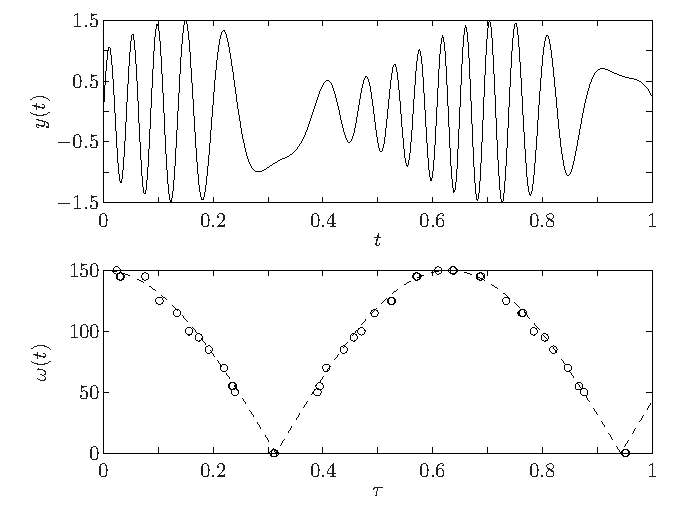
\includegraphics[width=.82\textwidth]{ch06-23.pdf}
\caption*{图6.23\quad 上：原信号。下：时频图。虚线表示原信号的瞬时频率 $\omega(t)=150|\cos(5t)|$。每个圆圈对应基追踪近似中选用的一个基元素，横轴为基元素的时刻指标 $\tau$，纵轴为频率指标 $\omega$。}
\end{figure}
相对误差为
\[\frac{(1/501)\sum_{i=1}^{501}(y(t_i)-\widehat y(t_i))^2}{(1/501)\sum_{i=1}^{501}y(t_i)^2}=2.6\cdot10^{-4}.\]

将非零系数的分布模式按时刻与频率绘出，就得到原始数据的时频分析。图6.23给出了这样的图，并同时绘出瞬时频率。图中可见，非零分量紧密跟随瞬时频率。

\subsection{用凸函数插值}
在一些特殊情形下，可以使用有限维凸优化，求解涉及无限维函数集合的插值问题。本节给出一个例子。

先问下面的问题：什么时候存在凸函数 $f:\R^k\to\R$，$\dom f=\R^k$，满足给定点 $u_i\in\R^k$ 上的插值条件
\[f(u_i)=y_i,\qquad i=1,\ldots,m?\]
（这里不要求 $f$ 位于任何有限维函数子空间中。）答案是：当且仅当存在 $g_1,\ldots,g_m$，使

% Source PDF page 352 (printed p. 338)
\begin{equation}y_j\ge y_i+g_i^\T(u_j-u_i),\qquad i,j=1,\ldots,m.\tag{6.19}\end{equation}
为证明这一点，先假设 $f$ 为凸函数，$\dom f=\R^k$，且 $f(u_i)=y_i$，$i=1,\ldots,m$。在每个 $u_i$ 处，都可找到向量 $g_i$，使对所有 $z$ 有
\begin{equation}f(z)\ge f(u_i)+g_i^\T(z-u_i).\tag{6.20}\end{equation}
如果 $f$ 可微，可取 $g_i=\nabla f(u_i)$；一般情况下，可以在 $(u_i,y_i)$ 处寻找 $\epi f$ 的一个支撑超平面来构造 $g_i$。（向量 $g_i$ 称为次梯度。）在 (6.20) 中取 $z=u_j$，即得到 (6.19)。

反之，假设 $g_1,\ldots,g_m$ 满足 (6.19)。对所有 $z\in\R^k$，定义
\[f(z)=\max_{i=1,\ldots,m}\bigl(y_i+g_i^\T(z-u_i)\bigr).\]
显然，$f$ 是分段线性的凸函数。不等式 (6.19) 蕴含 $f(u_i)=y_i$，$i=1,\ldots,m$。

利用这一结果，可以求解若干涉及用凸函数插值、逼近或求界的问题。

\subsubsection*{用凸函数拟合给定数据}
最简单的应用，也许是计算凸函数对给定数据 $(u_i,y_i)$（$i=1,\ldots,m$）的最小二乘拟合：
\[\begin{array}{ll}\text{最小化}&\displaystyle\sum_{i=1}^m(y_i-f(u_i))^2\\\text{约束条件}&f:\R^k\to\R\text{ 为凸函数},\quad\dom f=\R^k.\end{array}\]
这是一个无限维问题，因为变量 $f$ 位于 $\R^k$ 上的连续实值函数空间中。利用上述结果，可以将问题表述为
\[\begin{array}{ll}\text{最小化}&\displaystyle\sum_{i=1}^m(y_i-\widehat y_i)^2\\\text{约束条件}&\widehat y_j\ge\widehat y_i+g_i^\T(u_j-u_i),\quad i,j=1,\ldots,m,\end{array}\]
这是以 $\widehat y\in\R^m$ 和 $g_1,\ldots,g_m\in\R^k$ 为变量的 QP。当且仅当给定数据能由凸函数插值，即存在满足 $f(u_i)=y_i$ 的凸函数时，该问题最优值为零。图6.24给出一个例子。

\subsubsection*{对插值凸函数的取值求界}
另一个简单例子是：给定可由凸函数插值的数据 $(u_i,y_i)$，$i=1,\ldots,m$。对于另一个点 $u_0\in\R^k$，希望确定任意插值这些数据的凸函数 $f$ 的 $f(u_0)$ 可能取值范围。为求 $f(u_0)$ 的最小可能值，求解 LP
\[\begin{array}{ll}\text{最小化}&y_0\\\text{约束条件}&y_j\ge y_i+g_i^\T(u_j-u_i),\quad i,j=0,\ldots,m,\end{array}\]
变量为 $y_0\in\R$ 和 $g_0,\ldots,g_m\in\R^k$。将目标改为最大化 $y_0$（仍是 LP），就能找出插值给定数据的凸函数在 $u_0$ 处的最大可能值。

% Source PDF page 353 (printed p. 339)
\begin{figure}[htbp]\centering
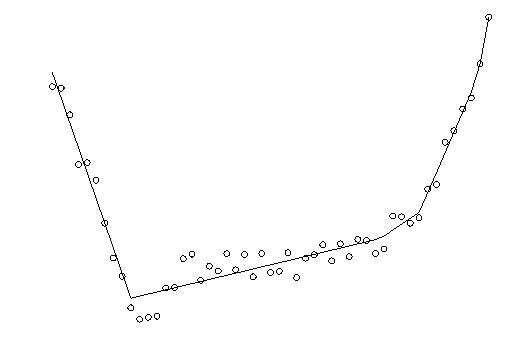
\includegraphics[width=.65\textwidth]{ch06-24.pdf}
\caption*{图6.24\quad 凸函数对以圆圈标出的数据的最小二乘拟合。图中的分段线性函数，在所有凸函数中使拟合误差的平方和最小。}
\end{figure}
\subsubsection*{用单调凸函数插值}
作为凸插值的扩展，可以考虑用凸且单调不减的函数插值。可以证明，存在凸函数 $f:\R^k\to\R$，$\dom f=\R^k$，满足插值条件
\[f(u_i)=y_i,\qquad i=1,\ldots,m,\]
且单调不减（$u\succeq v$ 时有 $f(u)\ge f(v)$），当且仅当存在 $g_1,\ldots,g_m\in\R^k$，使
\begin{equation}
\begin{gathered}
g_i\succeq0,\quad i=1,\ldots,m,\\
y_j\ge y_i+g_i^\T(u_j-u_i),\quad i,j=1,\ldots,m.
\end{gathered}\tag{6.21}
\end{equation}
也就是说，在凸插值条件 (6.19) 之外，再加上所有次梯度 $g_i$ 非负的条件。（见习题6.12。）

\subsubsection*{消费者偏好的推断与界定}
作为应用，考虑预测消费者偏好的问题。考虑由 $n$ 种消费品的不同数量组成的商品篮子。一个商品篮子用向量 $x\in[0,1]^n$ 表示，其中 $x_i$ 是第 $i$ 种商品的数量。假设数量已经归一化，使 $0\le x_i\le1$，其中 $x_i=0$、$x_i=1$ 分别是商品 $i$ 的最少与最多可能数量。给定两个商品篮子 $x$、$\widetilde x$，消费者可能更喜欢 $x$，可能更喜欢 $\widetilde x$，也可能认为两者同样有吸引力。考虑一位选择具有可重复性的模型消费者。

% Source PDF page 354 (printed p. 340)
按以下方式刻画消费者偏好。假设存在效用函数 $u:\R^n\to\R$，定义域为 $[0,1]^n$；$u(x)$ 衡量消费者从商品篮子 $x$ 中获得的效用。面对两个商品篮子，消费者选择效用较大的一个；如果两者效用相等，就无所谓选择哪一个。合理的假设是 $u$ 单调不减，这表示在其他商品数量保持不变时，消费者总希望任意一种商品更多一些。同样合理的是假设 $u$ 为凹函数，它刻画随着商品数量增加而出现的满足效应，即边际效用递减。

现在，假设给定一些消费者偏好数据，但不知道背后的效用函数 $u$。具体地，给定商品篮子集合 $a_1,\ldots,a_m\in[0,1]^n$，以及它们之间的一些偏好信息：
\begin{equation}
u(a_i)>u(a_j)\quad((i,j)\in\mathcal P),\qquad
u(a_i)\ge u(a_j)\quad((i,j)\in\mathcal P_{\rm weak}),\tag{6.22}
\end{equation}
其中 $\mathcal P,\mathcal P_{\rm weak}\subseteq\{1,\ldots,m\}\times\{1,\ldots,m\}$ 已知。$\mathcal P$ 给出已知严格偏好的集合：$(i,j)\in\mathcal P$ 表示已知消费者更喜欢篮子 $a_i$ 而非 $a_j$。集合 $\mathcal P_{\rm weak}$ 给出已知弱偏好：$(i,j)\in\mathcal P_{\rm weak}$ 表示 $a_i$ 比 $a_j$ 更受偏好，或者两者同样有吸引力。

先考虑如何判断数据是否一致，即是否存在满足 (6.22) 的凹且不减的效用函数 $u$。这等价于求解可行性问题
\begin{equation}
\begin{array}{ll}\text{寻找}&u\\\text{约束条件}&u:\R^n\to\R\text{ 为凹且不减的函数},\\&u(a_i)>u(a_j),\quad(i,j)\in\mathcal P,\\&u(a_i)\ge u(a_j),\quad(i,j)\in\mathcal P_{\rm weak},\end{array}\tag{6.23}
\end{equation}
以函数 $u$ 作为无限维优化变量。由于 (6.23) 中所有约束都是齐次的，可以将问题等价地写为
\begin{equation}
\begin{array}{ll}\text{寻找}&u\\\text{约束条件}&u:\R^n\to\R\text{ 为凹且不减的函数},\\&u(a_i)\ge u(a_j)+1,\quad(i,j)\in\mathcal P,\\&u(a_i)\ge u(a_j),\quad(i,j)\in\mathcal P_{\rm weak},\end{array}\tag{6.24}
\end{equation}
只使用非严格不等式。（显然，满足 (6.24) 的 $u$ 必满足 (6.23)；反之，若 $u$ 满足 (6.23)，则可将其缩放以满足 (6.24)。）再利用第339页的插值结果，可将该问题写成有限维线性规划可行性问题：
\begin{equation}
\begin{array}{ll}\text{寻找}&u_1,\ldots,u_m,g_1,\ldots,g_m\\\text{约束条件}&g_i\succeq0,\quad i=1,\ldots,m,\\&u_j\le u_i+g_i^\T(a_j-a_i),\quad i,j=1,\ldots,m,\\&u_i\ge u_j+1,\quad(i,j)\in\mathcal P,\\&u_i\ge u_j,\quad(i,j)\in\mathcal P_{\rm weak}.\end{array}\tag{6.25}
\end{equation}
求解这个线性规划可行性问题，就能确定是否存在与给定严格和非严格偏好集合一致的凹且不减的效用函数。

% Source PDF page 355 (printed p. 341)
如果 (6.25) 可行，至少存在一个这样的效用函数；事实上，由可行的 $u_1,\ldots,u_m,g_1,\ldots,g_m$ 还能构造一个分段线性效用函数。如果 (6.25) 不可行，就能断定：不存在与给定严格和非严格偏好集合一致的凹递增效用函数。

例如，假设已知消费者偏好 $\mathcal P$、$\mathcal P_{\rm weak}$ 与至少一个凹递增效用函数一致。考虑不属于 $\mathcal P$ 或 $\mathcal P_{\rm weak}$ 的一对 $(k,l)$，即篮子 $k$ 与 $l$ 之间的消费者偏好尚不明确。在某些情况下，即使不知道背后的偏好函数，也能推出二者之间的偏好。为此，在已知偏好 (6.22) 中加入不等式 $u(a_k)\le u(a_l)$，表示篮子 $l$ 比 $k$ 更受偏好，或两者同样有吸引力。然后求解包含额外弱偏好 $u(a_k)\le u(a_l)$ 的线性规划可行性问题 (6.25)。如果扩充后的偏好集合不可行，就意味着：任何与原始给定消费者偏好数据一致的凹不减效用函数，都必须满足 $u(a_k)>u(a_l)$。换言之，无须知道背后的效用函数，就能断定消费者更喜欢篮子 $k$ 而不是 $l$。

\begin{origexample}{6.9}
下面用一个简单数值例子说明上述讨论。考虑由两种商品组成的篮子，以便画出这些篮子。为生成消费者偏好数据 $\mathcal P$，在 $[0,1]^2$ 中随机生成40个点，然后用效用函数
\[u(x_1,x_2)=(1.1x_1^{1/2}+0.8x_2^{1/2})/1.9\]
比较它们。图6.25给出这些商品篮子以及效用函数 $u$ 的几条等值线。

现在，只用消费者偏好数据，当然不使用真实效用函数 $u$，将这40个篮子逐一与篮子 $a_0=(0.5,0.5)$ 比较。对每个原始篮子 $a_i$，求解上面描述的线性规划可行性问题，检查能否断定消费者更喜欢 $a_0$ 而非 $a_i$。同样，检查能否断定 $a_i$ 比 $a_0$ 更受偏好。对每个 $a_i$，有三种可能结果：确定更喜欢 $a_0$，确定更喜欢 $a_i$，或两个 LP 可行性问题均可行、因而无法作出结论。（这里“确定更喜欢”表示：对于任何与原始给定数据一致的凹不减效用函数，该偏好都成立。）

结果表明，与 $(0.5,0.5)$ 相比，21个篮子确定被排除，14个篮子确定更受偏好；依据消费者偏好数据，对剩余5个篮子无法作出结论。结果见图6.26。注意，仅用效用函数的单调性就能断定：$(0.5,0.5)$ 下方和左方的篮子会被排除，选择 $(0.5,0.5)$；同样，位于其上方和右方的点必定更受偏好。因此，对这17个点，无须求解可行性 LP (6.25)。不过，对另外两个象限中的23个点分类，需要使用凹性假设并求解可行性 LP (6.25)。
\end{origexample}

% Source PDF page 356 (printed p. 342)
\begin{figure}[htbp]\centering
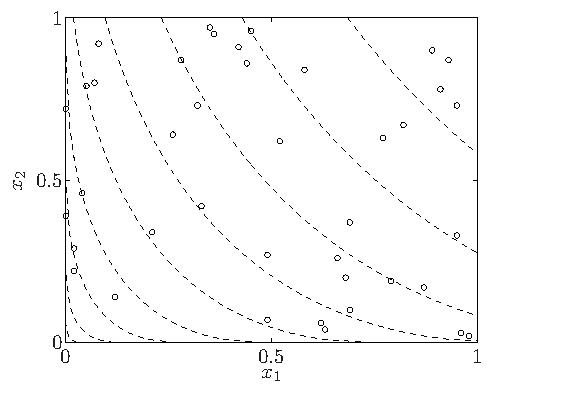
\includegraphics[width=.68\textwidth]{ch06-25.pdf}
\caption*{图6.25\quad 40个商品篮子 $a_1,\ldots,a_{40}$，以圆圈表示。虚线是真实效用函数 $u$ 的 $0.1,0.2,\ldots,0.9$ 等值线。利用该效用函数确定40个篮子之间的消费者偏好数据 $\mathcal P$。}
\end{figure}
\begin{figure}[htbp]\centering
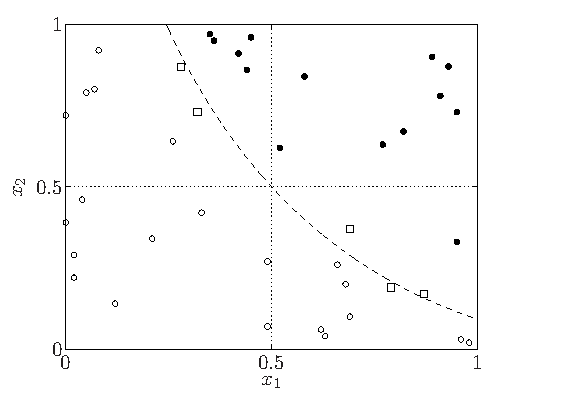
\includegraphics[width=.68\textwidth]{ch06-26.pdf}
\caption*{图6.26\quad 对新商品篮子 $a_0=(0.5,0.5)$，采用 LP (6.25) 进行消费者偏好分析的结果。若原始篮子确定被排除（$u(a_k)<u(a_0)$），画为空心圆；若确定更受偏好（$u(a_k)>u(a_0)$），画为实心黑圆；若无法作出结论，画为方框。经过 $(0.5,0.5)$ 的真实效用函数等值线用虚线表示。穿过 $(0.5,0.5)$ 的水平线和竖直线将 $[0,1]^2$ 划为四个象限。根据 $u$ 的单调性，右上象限中的点一定比 $(0.5,0.5)$ 更受偏好；同样，$(0.5,0.5)$ 一定比左下象限中的点更受偏好。对另外两个象限中的点，结果并不明显。}
\end{figure}

% Source PDF page 357 (printed p. 343)
\section*{文献说明}
\addcontentsline{toc}{section}{文献说明}
Huber [Hub64, Hub81] 分析了不同惩罚函数逼近的稳健性，并提出惩罚函数 (6.4)。对数障碍惩罚函数出现在控制理论中，用于系统闭环频率响应，有多种名称，例如 central $H_\infty$ 或 risk-averse control；见 Boyd 与 Barratt [BB91] 及其中的参考文献。

许多书籍讨论正则化逼近，包括 Tikhonov 与 Arsenin [TA77]、Hansen [Han98]。Tikhonov 正则化有时称为\emph{岭回归}（Golub 与 Van Loan [GL89, 第564页]）。采用 $\ell_1$ 范数正则化的最小二乘逼近，也称为 \emph{lasso}（Tibshirani [Tib96]）。Hastie、Tibshirani 与 Friedman [HTF01, 第3.4节] 讨论并比较了其他最小二乘正则化和回归向量选择方法。

Rudin、Osher 与 Fatemi [ROF92] 为图像重构引入了全变差去噪。

El Ghaoui 与 Lebret [EL97]，以及 Chandrasekaran、Golub、Gu 与 Sayed [CGGS98]，提出了范数有界不确定性下的稳健最小二乘问题（第321页）。El Ghaoui 与 Lebret 还给出了具有结构化不确定性的稳健最小二乘问题的 SDP 表述（第323页）。

Chen、Donoho 与 Saunders [CDS01] 讨论通过线性规划进行基追踪，并将 $\ell_1$ 范数正则化问题 (6.18) 称为\emph{基追踪去噪}。Meyer 与 Pratt [MP68] 是研究效用函数求界问题的一篇早期论文。

% Source PDF page 358 (printed p. 344)
\section*{习题}
\addcontentsline{toc}{section}{习题}
\subsection*{范数逼近与最小范数问题}
\paragraph{6.1} \emph{对数障碍惩罚的二次界。}令 $\phi:\R\to\R$ 为限制值 $a>0$ 的对数障碍惩罚函数：
\[\phi(u)=\begin{cases}-a^2\log(1-(u/a)^2),&|u|<a,\\\infty,&\text{其他情形}.\end{cases}\]
证明：若 $u\in\R^m$ 满足 $\norm u_\infty<a$，则
\[\norm u_2^2\le\sum_{i=1}^m\phi(u_i)\le\frac{\phi(\norm u_\infty)}{\norm u_\infty^2}\norm u_2^2.\]
这意味着，如果 $\norm u_\infty$ 相对于 $a$ 较小，$\norm u_2^2$ 就很好地近似 $\sum_{i=1}^m\phi(u_i)$。例如，若 $\norm u_\infty/a=0.25$，则
\[\norm u_2^2\le\sum_{i=1}^m\phi(u_i)\le1.033\cdot\norm u_2^2.\]

\paragraph{6.2} \emph{用常向量作 $\ell_1$、$\ell_2$ 和 $\ell_\infty$ 范数逼近。}对于只有一个标量变量 $x\in\R$ 的范数逼近问题
\[\text{最小化}\quad\norm{x\one-b},\]
采用 $\ell_1$、$\ell_2$ 和 $\ell_\infty$ 范数时，其解分别是什么？

\paragraph{6.3} 将下列逼近问题表述为 LP、QP、SOCP 或 SDP。问题数据为 $A\in\R^{m\times n}$ 和 $b\in\R^m$，$A$ 的各行记为 $a_i^\T$。
\begin{enumerate}[label=(\alph*)]
\item \emph{死区线性惩罚逼近：}最小化 $\sum_{i=1}^m\phi(a_i^\T x-b_i)$，其中
\[\phi(u)=\begin{cases}0,&|u|\le a,\\|u|-a,&|u|>a,\end{cases}\]
且 $a>0$。
\item \emph{对数障碍惩罚逼近：}最小化 $\sum_{i=1}^m\phi(a_i^\T x-b_i)$，其中
\[\phi(u)=\begin{cases}-a^2\log(1-(u/a)^2),&|u|<a,\\\infty,&|u|\ge a,\end{cases}\]
且 $a>0$。
\item \emph{Huber 惩罚逼近：}最小化 $\sum_{i=1}^m\phi(a_i^\T x-b_i)$，其中
\[\phi(u)=\begin{cases}u^2,&|u|\le M,\\M(2|u|-M),&|u|>M,\end{cases}\]
且 $M>0$。
\item \emph{对数 Chebyshev 逼近：}最小化 $\max_{i=1,\ldots,m}|\log(a_i^\T x)-\log b_i|$，假定 $b\succ0$。一个等价的凸形式为
\[\begin{array}{ll}\text{最小化}&t\\\text{约束条件}&1/t\le a_i^\T x/b_i\le t,\quad i=1,\ldots,m,\end{array}\]
变量为 $x\in\R^n$、$t\in\R$，定义域为 $\R^n\times\R_{++}$。
\end{enumerate}

% Source PDF page 359 (printed p. 345)
\begin{enumerate}[label=(\alph*),start=5]
\item \emph{最小化最大的 $k$ 个残差之和：}
\[\begin{array}{ll}\text{最小化}&\displaystyle\sum_{i=1}^k|r|_{[i]}\\\text{约束条件}&r=Ax-b,\end{array}\]
其中 $|r|_{[1]}\ge|r|_{[2]}\ge\cdots\ge|r|_{[m]}$ 是将 $|r_1|,|r_2|,\ldots,|r_m|$ 按降序排列的结果。（$k=1$ 时化为 $\ell_\infty$ 范数逼近；$k=m$ 时化为 $\ell_1$ 范数逼近。）\emph{提示：}见习题5.19。
\end{enumerate}

\paragraph{6.4} \emph{$\ell_1$ 范数逼近的可微近似。}函数 $\phi(u)=(u^2+\epsilon)^{1/2}$，其中参数 $\epsilon>0$，有时用作绝对值函数 $|u|$ 的可微近似。为了近似求解 $\ell_1$ 范数逼近问题
\begin{equation}\text{最小化}\quad\norm{Ax-b}_1,\tag{6.26}\end{equation}
其中 $A\in\R^{m\times n}$，转而求解问题
\begin{equation}\text{最小化}\quad\sum_{i=1}^m\phi(a_i^\T x-b_i),\tag{6.27}\end{equation}
其中 $a_i^\T$ 是 $A$ 的第 $i$ 行。假设 $\rank A=n$。

令 $p^\star$ 为 $\ell_1$ 范数逼近问题 (6.26) 的最优值，$\widehat x$ 为近似问题 (6.27) 的最优解，$\widehat r$ 为对应残差，$\widehat r=A\widehat x-b$。
\begin{enumerate}[label=(\alph*)]
\item 证明 $p^\star\ge\sum_{i=1}^m\widehat r_i^2/(\widehat r_i^2+\epsilon)^{1/2}$。
\item 证明
\[\norm{A\widehat x-b}_1\le p^\star+\sum_{i=1}^m|\widehat r_i|\left(1-\frac{|\widehat r_i|}{(\widehat r_i^2+\epsilon)^{1/2}}\right).\]
\end{enumerate}
（计算 $\widehat x$ 后求出右端，就得到 $\widehat x$ 对 $\ell_1$ 范数逼近问题的次优程度的一个界。）

\paragraph{6.5} \emph{最短长度逼近。}考虑问题
\[\begin{array}{ll}\text{最小化}&\operatorname{length}(x)\\\text{约束条件}&\norm{Ax-b}\le\epsilon,\end{array}\]
其中 $\operatorname{length}(x)=\min\{k\mid x_i=0\text{ 对 }i>k\}$。问题变量为 $x\in\R^n$，参数为 $A\in\R^{m\times n}$、$b\in\R^m$、$\epsilon>0$。在回归中，要求按原有顺序取尽可能少的 $A$ 的列，以在误差 $\epsilon$ 内逼近向量 $b$。

证明这是一个拟凸优化问题。

\paragraph{6.6} \emph{一些惩罚函数逼近问题的对偶。}对于以下惩罚函数 $\phi:\R\to\R$，推导问题
\[\begin{array}{ll}\text{最小化}&\displaystyle\sum_{i=1}^m\phi(r_i)\\\text{约束条件}&r=Ax-b\end{array}\]
的拉格朗日对偶。变量为 $x\in\R^n$、$r\in\R^m$。
\begin{enumerate}[label=(\alph*)]
\item 死区线性惩罚（死区宽度 $a=1$）：
\[\phi(u)=\begin{cases}0,&|u|\le1,\\|u|-1,&|u|>1.\end{cases}\]
\item Huber 惩罚（$M=1$）：
\[\phi(u)=\begin{cases}u^2,&|u|\le1,\\2|u|-1,&|u|>1.\end{cases}\]
\end{enumerate}

% Source PDF page 360 (printed p. 346)
\begin{enumerate}[label=(\alph*),start=3]
\item 对数障碍（限制值 $a=1$）：
\[\phi(u)=-\log(1-u^2),\qquad\dom\phi=(-1,1).\]
\item 相对 $1$ 的偏差：
\[\phi(u)=\max\{u,1/u\}=\begin{cases}u,&u\ge1,\\1/u,&u\le1,\end{cases}\]
其中 $\dom\phi=\R_{++}$。
\end{enumerate}

\subsection*{正则化与稳健逼近}
\paragraph{6.7} \emph{采用欧几里得范数的双准则优化。}考虑双准则优化问题
\[\text{相对于 }\R_+^2\text{ 最小化}\quad(\norm{Ax-b}_2^2,\norm x_2^2),\]
其中 $A\in\R^{m\times n}$ 的秩为 $r$，$b\in\R^m$。说明如何从 $A$ 的奇异值分解
\[A=U\diag(\sigma)V^\T=\sum_{i=1}^r\sigma_i u_i v_i^\T\]
求出以下各问题的解（见第A.5.4节）。
\begin{enumerate}[label=(\alph*)]
\item Tikhonov 正则化：最小化 $\norm{Ax-b}_2^2+\delta\norm x_2^2$。
\item 在 $\norm x_2^2=\gamma$ 下最小化 $\norm{Ax-b}_2^2$。
\item 在 $\norm x_2^2=\gamma$ 下最大化 $\norm{Ax-b}_2^2$。
\end{enumerate}
其中 $\delta$ 和 $\gamma$ 是正参数。

你的结果给出计算最优权衡曲线及该双准则问题可达值集合的高效方法。

\paragraph{6.8} 将下列稳健逼近问题表述为 LP、QP、SOCP 或 SDP。对每个小题，分别考虑 $\ell_1$、$\ell_2$ 和 $\ell_\infty$ 范数。
\begin{enumerate}[label=(\alph*)]
\item 有限参数取值集合上的随机稳健逼近，即范数和问题
\[\text{最小化}\quad\sum_{i=1}^k p_i\norm{A_ix-b},\]
其中 $p\succeq0$、$\one^\T p=1$。（见第6.4.1节。）
\item 系数有界时的最坏情形稳健逼近：
\[\text{最小化}\quad\sup_{A\in\mathcal A}\norm{Ax-b},\]
其中
\[\mathcal A=\{A\in\R^{m\times n}\mid l_{ij}\le a_{ij}\le u_{ij},\ i=1,\ldots,m,\ j=1,\ldots,n\}.\]
不确定集由 $A$ 各元素的上下界描述。假设 $l_{ij}<u_{ij}$。
\item 多面体不确定性下的最坏情形稳健逼近：
\[\text{最小化}\quad\sup_{A\in\mathcal A}\norm{Ax-b},\]
其中
\[\mathcal A=\{[a_1\ \cdots\ a_m]^\T\mid C_ia_i\preceq d_i,\ i=1,\ldots,m\}.\]
给出每一行可能取值的多面体 $\mathcal P_i=\{a_i\mid C_ia_i\preceq d_i\}$ 来描述不确定性。参数 $C_i\in\R^{p_i\times n}$、$d_i\in\R^{p_i}$，$i=1,\ldots,m$ 已知。假设多面体 $\mathcal P_i$ 非空且有界。
\end{enumerate}

% Source PDF page 361 (printed p. 347)
\subsection*{函数拟合与插值}
\paragraph{6.9} \emph{极小极大有理函数拟合。}证明以下问题为拟凸问题：
\[\text{最小化}\quad\max_{i=1,\ldots,k}\left|\frac{p(t_i)}{q(t_i)}-y_i\right|,\]
其中
\[p(t)=a_0+a_1t+a_2t^2+\cdots+a_mt^m,\qquad q(t)=1+b_1t+\cdots+b_nt^n,\]
目标函数的定义域为
\[\mathcal D=\{(a,b)\in\R^{m+1}\times\R^n\mid q(t)>0,\ \alpha\le t\le\beta\}.\]
该问题用有理函数 $p(t)/q(t)$ 拟合给定数据，并要求分母多项式在区间 $[\alpha,\beta]$ 上为正。优化变量为分子、分母系数 $a_i$、$b_i$。插值点 $t_i\in[\alpha,\beta]$ 和期望函数值 $y_i$（$i=1,\ldots,k$）已知。

\paragraph{6.10} \emph{用凹、非负、不减的二次函数拟合数据。}给定数据
\[x_1,\ldots,x_N\in\R^n,\qquad y_1,\ldots,y_N\in\R,\]
希望用如下形式的二次函数拟合：
\[f(x)=(1/2)x^\T Px+q^\T x+r,\]
其中 $P\in\mathbf S^n$、$q\in\R^n$、$r\in\R$ 是模型参数，因而也是拟合问题的变量。

模型只在盒 $\mathcal B=\{x\in\R^n\mid l\preceq x\preceq u\}$ 上使用。可以假设 $l\prec u$，并且给定数据点 $x_i$ 均在该盒中。

以简单的误差平方和
\[\sum_{i=1}^N(f(x_i)-y_i)^2\]
作为拟合准则，同时对函数 $f$ 施加几个约束。首先，$f$ 必须凹。其次，$f$ 在 $\mathcal B$ 上非负，即对所有 $z\in\mathcal B$，有 $f(z)\ge0$。第三，$f$ 在 $\mathcal B$ 上不减，即当 $z,\widetilde z\in\mathcal B$ 满足 $z\preceq\widetilde z$ 时，有 $f(z)\le f(\widetilde z)$。

说明如何将该拟合问题表述为凸问题，并尽可能简化表述。

\paragraph{6.11} \emph{最小二乘方向插值。}假设 $F_1,\ldots,F_n:\R^k\to\R^p$，构造线性组合 $F:\R^k\to\R^p$：
\[F(u)=x_1F_1(u)+\cdots+x_nF_n(u),\]
其中 $x$ 是插值问题的变量。

要求 $\angle(F(v_j),q_j)=0$，$j=1,\ldots,m$，其中 $q_j$ 是给定的 $\R^p$ 中的向量，假定 $\norm{q_j}_2=1$。也就是说，要求 $F$ 在点 $v_j$ 处具有指定方向。为了确保 $F(v_j)$ 非零（为零时夹角无定义），加入最小长度约束 $\norm{F(v_j)}_2\ge\epsilon$，$j=1,\ldots,m$，其中 $\epsilon>0$ 已知。

说明如何用凸优化寻找满足上述方向及最小长度条件、并使 $\norm x_2$ 最小的 $x$。

\paragraph{6.12} \emph{用单调函数插值。}如果 $u\succeq v$ 时有 $f(u)\ge f(v)$，函数 $f:\R^k\to\R$ 就是相对于 $\R_+^k$ 单调不减的。

% Source PDF page 362 (printed p. 348)
\begin{enumerate}[label=(\alph*)]
\item 证明：存在满足 $f(u_i)=y_i$（$i=1,\ldots,m$）的单调不减函数 $f:\R^k\to\R$，当且仅当
\[u_i\succeq u_j\text{ 时有 }y_i\ge y_j,\qquad i,j=1,\ldots,m.\]
\item 证明：存在满足 $\dom f=\R^k$ 和 $f(u_i)=y_i$（$i=1,\ldots,m$）的凸单调不减函数 $f:\R^k\to\R$，当且仅当存在 $g_i\in\R^k$（$i=1,\ldots,m$），使
\[g_i\succeq0,\quad i=1,\ldots,m,\qquad y_j\ge y_i+g_i^\T(u_j-u_i),\quad i,j=1,\ldots,m.\]
\end{enumerate}

\paragraph{6.13} \emph{用拟凸函数插值。}证明：存在满足 $f(u_i)=y_i$（$i=1,\ldots,m$）的拟凸函数 $f:\R^k\to\R$，当且仅当存在 $g_i\in\R^k$（$i=1,\ldots,m$），使
\[y_j<y_i\text{ 时有 }g_i^\T(u_j-u_i)\le-1,\qquad i,j=1,\ldots,m.\]

\paragraph{6.14} [Nes00] \emph{用正实函数插值。}假设 $z_1,\ldots,z_n\in\C$ 是 $n$ 个互异点，且 $|z_i|>1$。定义 $K_{\rm np}$ 为满足下列条件的向量 $y\in\C^n$ 的集合：存在函数 $f:\C\to\C$，满足
\begin{itemize}
\item $f$ 为正实函数，即在单位圆外（$|z|>1$）解析，且实部在单位圆外非负（$|z|>1$ 时 $\operatorname{Re}f(z)\ge0$）。
\item $f$ 满足插值条件
\[f(z_1)=y_1,\qquad f(z_2)=y_2,\quad\ldots,\quad f(z_n)=y_n.\]
\end{itemize}
若正实函数集记为 $\mathcal F$，则
\[K_{\rm np}=\{y\in\C^n\mid\exists f\in\mathcal F,\ y_k=f(z_k),\ k=1,\ldots,n\}.\]
\begin{enumerate}[label=(\alph*)]
\item 可以证明，$f$ 为正实函数，当且仅当存在不减函数 $\rho$，使对所有 $|z|>1$ 有
\[f(z)=\mathrm i\operatorname{Im}f(\infty)+\int_0^{2\pi}\frac{e^{\mathrm i\theta}+z^{-1}}{e^{\mathrm i\theta}-z^{-1}}\,d\rho(\theta),\]
其中 $\mathrm i=\sqrt{-1}$（见 [KN77, 第389页]）。用这一表示证明 $K_{\rm np}$ 是闭凸锥。
\item 在向量 $x,y\in\C^n$ 之间使用内积 $\operatorname{Re}(x^{\HH}y)$，其中 $x^{\HH}$ 表示 $x$ 的共轭转置。证明 $K_{\rm np}$ 的对偶锥为
\[K_{\rm np}^*=\left\{x\in\C^n\;\middle|\;\begin{gathered}
\operatorname{Im}(\one^\T x)=0,\\
\operatorname{Re}\left(\sum_{l=1}^n x_l\frac{e^{-\mathrm i\theta}+\overline z_l^{-1}}{e^{-\mathrm i\theta}-\overline z_l^{-1}}\right)\ge0\quad\forall\theta\in[0,2\pi]
\end{gathered}\right\}.\]
\item 证明
\[K_{\rm np}^*=\left\{x\in\C^n\;\middle|\;\exists Q\in\mathbf H_+^n,\quad x_l=\sum_{k=1}^n\frac{Q_{kl}}{1-z_k^{-1}\overline z_l^{-1}},\quad l=1,\ldots,n\right\},\]
其中 $\mathbf H_+^n$ 表示所有 $n\times n$ 厄米半正定矩阵的集合。

使用以下结论，称为 Riesz--Fej\'er 定理，见 [KN77, 第60页]：形如
\[\sum_{k=0}^n(y_ke^{-\mathrm ik\theta}+\overline y_ke^{\mathrm ik\theta})\]
的函数对所有 $\theta$ 非负，当且仅当存在 $a_0,\ldots,a_n\in\C$，使
\[\sum_{k=0}^n(y_ke^{-\mathrm ik\theta}+\overline y_ke^{\mathrm ik\theta})=\left|\sum_{k=0}^n a_ke^{\mathrm ik\theta}\right|^2.\]
\end{enumerate}

% Source PDF page 363 (printed p. 349)
\begin{enumerate}[label=(\alph*),start=4]
\item 证明 $K_{\rm np}=\{y\in\C^n\mid P(y)\succeq0\}$，其中 $P(y)\in\mathbf H^n$ 定义为
\[P(y)_{kl}=\frac{y_k+\overline y_l}{1-z_k^{-1}\overline z_l^{-1}},\qquad l,k=1,\ldots,n.\]
矩阵 $P(y)$ 称为与点 $z_k,y_k$ 对应的 Nevanlinna--Pick 矩阵。

\emph{提示：}由 (a) 知，$K_{\rm np}$ 是闭凸锥，因此 $K_{\rm np}=K_{\rm np}^{**}$。
\item 作为应用，将下列问题表述为凸优化问题：
\[\begin{array}{ll}\text{最小化}&\displaystyle\sum_{k=1}^n|f(z_k)-w_k|^2\\\text{约束条件}&f\in\mathcal F.\end{array}\]
问题数据为 $n$ 个满足 $|z_k|>1$ 的点 $z_k$，以及 $n$ 个复数 $w_1,\ldots,w_n$。在所有正实函数 $f$ 上优化。
\end{enumerate}

% Source PDF page 364 (printed p. 350)
% This source page is blank.


\chapter{统计估计}
% Source PDF page 365 (printed p. 351)
\section{参数化分布估计}
\subsection{最大似然估计}
考虑 $\R^m$ 上由向量 $x\in\R^n$ 索引的一族概率分布，其密度为 $p_x(\cdot)$。固定 $y\in\R^m$，将 $p_x(y)$ 看成 $x$ 的函数时，称其为\emph{似然函数}。使用它的对数更方便，这个对数称为\emph{对数似然函数}，记作 $l$：
\[
 l(x)=\log p_x(y).
\]
参数 $x$ 的取值往往有约束，可以表示关于 $x$ 的先验知识，也可以表示似然函数的定义域。这些约束可以显式给出，也可以包含在似然函数中：只要 $x$ 不满足先验信息约束，就对所有 $y$ 令 $p_x(y)=0$。因此，对违反先验信息约束的参数 $x$，可以将对数似然函数赋值为 $-\infty$。

现在，考虑根据从分布中观测到的一个样本 $y$ 估计参数 $x$。一种广泛使用的方法是\emph{最大似然}（ML）估计，将 $x$ 估计为
\[
 \widehat x_{\mathrm{ml}}=\argmax_xp_x(y)=\argmax_xl(x),
\]
即选择使观测值 $y$ 的似然函数或对数似然函数最大的参数值作为估计。如果存在关于 $x$ 的先验信息，例如 $x\in C\subseteq\R^n$，则可显式加入约束 $x\in C$，或者对 $x\notin C$ 重新定义 $p_x(y)=0$，从而隐式施加这一约束。

寻找参数向量 $x$ 的最大似然估计，可以写为
\begin{equation}
\begin{array}{ll}
\text{最大化}&l(x)=\log p_x(y)\\
\text{满足}&x\in C,
\end{array}\tag{7.1}
\end{equation}
其中 $x\in C$ 表示参数向量的先验信息或其他约束。在该优化问题中，向量 $x\in\R^n$，即概率密度中的参数，是优化变量；向量 $y\in\R^m$，即观测样本，是问题参数。

% Source PDF page 366 (printed p. 352)
如果对每个 $y$，对数似然函数 $l$ 都凹，而且集合 $C$ 能用线性等式和凸不等式约束描述，那么最大似然估计问题（7.1）就是凸优化问题。许多估计问题都属于这种情形，可以用凸优化计算ML估计。

\subsubsection*{具有独立同分布噪声的线性测量}
考虑线性测量模型
\[
 y_i=a_i^{\T}x+v_i,\qquad i=1,\ldots,m,
\]
其中 $x\in\R^n$ 是待估参数向量，$y_i\in\R$ 为测量或观测量，$v_i$ 是测量误差或噪声。假设 $v_i$ 独立同分布（IID），在 $\R$ 上的密度为 $p$，则似然函数为
\[
 p_x(y)=\prod_{i=1}^mp(y_i-a_i^{\T}x),
\]
从而对数似然函数为
\[
 l(x)=\log p_x(y)=\sum_{i=1}^m\log p(y_i-a_i^{\T}x).
\]
ML估计为下列问题的任意最优点：
\begin{equation}
 \text{最大化}\quad\sum_{i=1}^m\log p(y_i-a_i^{\T}x),\tag{7.2}
\end{equation}
变量为 $x$。如果密度 $p$ 对数凹，则该问题凸，并具有罚函数逼近问题的形式，罚函数为 $-\log p$，见第294页（6.2）。

\begin{origexample}{7.1}
\textbf{几种常见噪声密度的ML估计。}
\begin{itemize}
\item \emph{高斯噪声。}若 $v_i$ 服从零均值、方差为 $\sigma^2$ 的高斯分布，其密度为
\[
 p(z)=(2\pi\sigma^2)^{-1/2}e^{-z^2/(2\sigma^2)},
\]
对数似然函数为
\[
 l(x)=-(m/2)\log(2\pi\sigma^2)-\frac1{2\sigma^2}\norm{Ax-y}_2^2,
\]
其中 $A$ 的各行为 $a_1^{\T},\ldots,a_m^{\T}$。因此，$x$ 的ML估计为 $x_{\mathrm{ml}}=\argmin_x\norm{Ax-y}_2^2$，即最小二乘逼近问题的解。
\item \emph{Laplace噪声。}若 $v_i$ 服从Laplace分布，密度为 $p(z)=(1/2a)e^{-\abs z/a}$，其中 $a>0$，则ML估计为 $\widehat x=\argmin_x\norm{Ax-y}_1$，即 $\ell_1$ 范数逼近问题的解。
\item \emph{均匀噪声。}若 $v_i$ 在 $[-a,a]$ 上均匀分布，则在该区间有 $p(z)=1/(2a)$，任意满足 $\norm{Ax-y}_\infty\le a$ 的 $x$ 都是一个ML估计。
\end{itemize}
\end{origexample}

% Source PDF page 367 (printed p. 353)
\subsubsection*{罚函数逼近的ML解释}
反过来，任意罚函数逼近问题
\[
 \text{最小化}\quad\sum_{i=1}^m\phi(b_i-a_i^{\T}x)
\]
都可以解释为测量值为 $b$、噪声密度为
\[
 p(z)=\frac{e^{-\phi(z)}}{\int e^{-\phi(u)}\,\mathrm du}
\]
的最大似然估计问题。这个观察为罚函数逼近提供了统计解释。例如，假设罚函数 $\phi$ 在较大取值处增长极快，意味着对大的残差赋予很大的代价或惩罚。相应噪声密度 $p$ 的尾部会很小；ML估计器将尽可能避免产生大残差，因为这些残差对应极不可能发生的事件。

也可从最大似然估计的角度理解，为什么 $\ell_1$ 范数逼近对大误差稳健。$\ell_1$ 范数逼近对应Laplace噪声密度下的最大似然估计，$\ell_2$ 范数逼近对应高斯噪声密度下的最大似然估计。Laplace密度的尾部比高斯密度更大，也就是说，Laplace分布下出现很大 $v_i$ 的概率远高于高斯分布。因此，相应最大似然方法预期会遇到更多的大残差。

\subsubsection*{Poisson分布的计数问题}
许多问题中的随机变量 $y$ 取非负整数值，服从均值 $\mu>0$ 的Poisson分布：
\[
 \Prob(y=k)=\frac{e^{-\mu}\mu^k}{k!}.
\]
$y$ 常常表示某段时间内Poisson过程的事件次数，例如光子到达次数、交通事故数等。

在一个简单的统计模型中，将均值 $\mu$ 建模为向量 $u\in\R^n$ 的仿射函数：
\[
 \mu=a^{\T}u+b.
\]
$u$ 称为\emph{解释变量}向量，$a\in\R^n$ 和 $b\in\R$ 称为\emph{模型参数}。例如，若 $y$ 是某地区某时段的交通事故数，$u_1$ 可以是该时段经过该地区的总交通流量，$u_2$ 可以是该时段该地区的降雨量，等等。

给定若干观测对 $(u_i,y_i)$，$i=1,\ldots,m$，其中 $y_i$ 是解释变量取 $u_i\in\R^n$ 时观测到的 $y$。任务是由这些数据找到模型参数 $a\in\R^n$、$b\in\R$ 的最大似然估计。

% Source PDF page 368 (printed p. 354)
似然函数为
\[
 \prod_{i=1}^m\frac{(a^{\T}u_i+b)^{y_i}\exp(-(a^{\T}u_i+b))}{y_i!},
\]
所以对数似然函数为
\[
 l(a,b)=\sum_{i=1}^m\bigl(y_i\log(a^{\T}u_i+b)-(a^{\T}u_i+b)-\log(y_i!)\bigr).
\]
通过求解凸优化问题
\[
 \text{最大化}\quad\sum_{i=1}^m\bigl(y_i\log(a^{\T}u_i+b)-(a^{\T}u_i+b)\bigr),
\]
便可找到 $a$、$b$ 的ML估计，变量为 $a,b$。

\subsubsection*{Logistic回归}
考虑随机变量 $y\in\{0,1\}$，满足
\[
 \Prob(y=1)=p,\qquad\Prob(y=0)=1-p,
\]
其中 $p\in[0,1]$，假设它依赖解释变量向量 $u\in\R^n$。例如，$y=1$ 可以表示某人患某种疾病，患病概率为 $p$。将 $p$ 建模为解释变量 $u$ 的函数，这些解释变量可以是体重、年龄、身高、血压及其他医学相关变量。

\emph{Logistic模型}的形式为
\begin{equation}
 p=\frac{\exp(a^{\T}u+b)}{1+\exp(a^{\T}u+b)},\tag{7.3}
\end{equation}
其中模型参数 $a\in\R^n$、$b\in\R$ 确定概率 $p$ 如何随解释变量 $u$ 变化。

现给定解释变量 $u_1,\ldots,u_m\in\R^n$ 及相应结果 $y_1,\ldots,y_m\in\{0,1\}$ 组成的数据，任务是找到模型参数 $a\in\R^n$、$b\in\R$ 的最大似然估计。求 $a,b$ 的ML估计有时称为\emph{Logistic回归}。

可重排数据，使 $u_1,\ldots,u_q$ 对应 $y=1$，$u_{q+1},\ldots,u_m$ 对应 $y=0$。似然函数为
\[
 \prod_{i=1}^q p_i\prod_{i=q+1}^m(1-p_i),
\]
其中 $p_i$ 由解释变量取 $u_i$ 的Logistic模型给出。对数似然函数为
\[
 l(a,b)=\sum_{i=1}^q\log p_i+\sum_{i=q+1}^m\log(1-p_i).
\]

% Source PDF page 369 (printed p. 355)
\begin{figure}[htbp]\centering
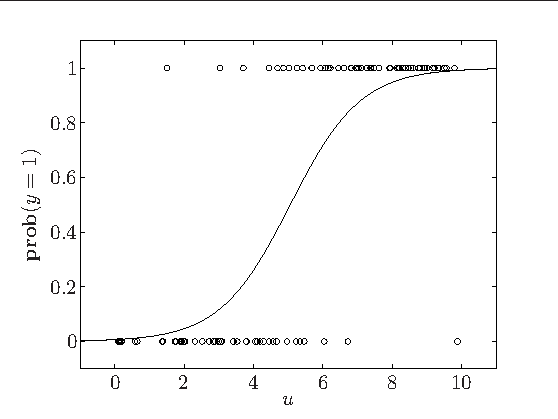
\includegraphics[width=.70\textwidth]{figures/ch07-figure-1.pdf}
\caption*{图7.1\quad Logistic回归。圆圈表示50个点 $(u_i,y_i)$，其中 $u_i\in\R$ 是解释变量，$y_i\in\{0,1\}$ 是结果。数据表明，当 $u$ 小于约5时，结果更可能为 $y=0$；当 $u$ 大于约5时，更可能为 $y=1$。此外，当 $u$ 小于约2时，$y=0$ 的可能性很高；当 $u$ 大于约8时，$y=1$ 的可能性很高。实线为最大似然参数 $a,b$ 对应的 $\Prob(y=1)=\exp(au+b)/(1+\exp(au+b))$。这个最大似然模型与我们对数据的非正式观察一致。}
\end{figure}
继续化简得
\[
\begin{aligned}
 l(a,b)&=\sum_{i=1}^q\log\frac{\exp(a^{\T}u_i+b)}{1+\exp(a^{\T}u_i+b)}
       +\sum_{i=q+1}^m\log\frac1{1+\exp(a^{\T}u_i+b)}\\
 &=\sum_{i=1}^q(a^{\T}u_i+b)-\sum_{i=1}^m\log(1+\exp(a^{\T}u_i+b)).
\end{aligned}
\]
由于 $l$ 关于 $a,b$ 凹，Logistic回归可作为凸优化问题求解。图7.1给出了 $u\in\R$ 时的一个例子。

\subsubsection*{高斯变量的协方差估计}
设 $y\in\R^n$ 是零均值高斯随机变量，协方差矩阵为 $R=\E yy^{\T}$，则其密度为
\[
 p_R(y)=(2\pi)^{-n/2}\det(R)^{-1/2}\exp(-y^{\T}R^{-1}y/2),
\]
其中 $R\in\mathbf S_{++}^n$。我们希望根据从分布中抽取的 $N$ 个独立样本 $y_1,\ldots,y_N\in\R^n$，并利用关于 $R$ 的先验知识，估计协方差矩阵 $R$。

对数似然函数为
\[
 l(R)=\log p_R(y_1,\ldots,y_N).
\]

% Source PDF page 370 (printed p. 356)
展开得到
\[
\begin{aligned}
 l(R)&=-(Nn/2)\log(2\pi)-(N/2)\log\det R
       -(1/2)\sum_{k=1}^N y_k^{\T}R^{-1}y_k\\
 &=-(Nn/2)\log(2\pi)-(N/2)\log\det R
       -(N/2)\tr(R^{-1}Y),
\end{aligned}
\]
其中
\[
 Y=\frac1N\sum_{k=1}^N y_ky_k^{\T}
\]
是 $y_1,\ldots,y_N$ 的样本协方差。该对数似然函数关于 $R$ 不凹，尽管它在定义域 $\mathbf S_{++}^n$ 的某个子集上凹，见习题7.4；但变量变换可得到凹的对数似然函数。用 $S=R^{-1}$ 表示协方差的逆，称其为\emph{信息矩阵}。以 $S$ 代替 $R$ 作为新参数，对数似然函数成为
\[
 l(S)=-(Nn/2)\log(2\pi)+(N/2)\log\det S-(N/2)\tr(SY),
\]
它关于 $S$ 凹。

因此，求解
\begin{equation}
\begin{array}{ll}
\text{最大化}&\log\det S-\tr(SY)\\
\text{满足}&S\in\mathcal S
\end{array}\tag{7.4}
\end{equation}
即可得到 $S$，进而得到 $R$ 的ML估计，其中集合 $\mathcal S$ 表示对 $S=R^{-1}$ 的先验知识，此外还有隐式约束 $S\in\mathbf S_{++}^n$。目标函数凹，因此当 $\mathcal S$ 能由线性等式与凸不等式约束描述时，该问题凸。

先考察除 $R\succ0$ 外，对 $R$，从而对 $S$，不作其他先验假设的情形。这时（7.4）可解析求解。目标的梯度为 $S^{-1}-Y$，所以当 $Y\in\mathbf S_{++}^n$ 时，最优 $S$ 满足 $S^{-1}=Y$。如果 $Y\notin\mathbf S_{++}^n$，对数似然函数上无界。因此，不对 $R$ 作先验假设时，协方差的最大似然估计就是样本协方差：$\widehat R_{\mathrm{ml}}=Y$。

再考虑可表示为信息矩阵 $S$ 的凸约束的一些 $R$ 约束。$R$ 的矩阵下界与上界
\[
 L\preceq R\preceq U,
\]
其中 $L,U$ 对称正定，可以写成
\[
 U^{-1}\preceq R^{-1}\preceq L^{-1}.
\]
关于 $R$ 的条件数约束
\[
 \lambda_{\max}(R)\le\kappa_{\max}\lambda_{\min}(R)
\]
可写为
\[
 \lambda_{\max}(S)\le\kappa_{\max}\lambda_{\min}(S).
\]

% Source PDF page 371 (printed p. 357)
这等价于存在 $u>0$，使 $uI\preceq S\preceq\kappa_{\max}uI$。因此，带 $R$ 条件数约束的ML估计，可以通过求解凸问题
\begin{equation}
\begin{array}{ll}
\text{最大化}&\log\det S-\tr(SY)\\
\text{满足}&uI\preceq S\preceq\kappa_{\max}uI
\end{array}\tag{7.5}
\end{equation}
得到，变量为 $S\in\mathbf S^n$ 和 $u\in\R$。

另一个例子是，对底层随机向量 $y$ 的若干线性函数的方差给出上界：
\[
 \E(c_i^{\T}y)^2\le\alpha_i,\qquad i=1,\ldots,K.
\]
这些先验假设可以表示为
\[
 \E(c_i^{\T}y)^2=c_i^{\T}Rc_i=c_i^{\T}S^{-1}c_i\le\alpha_i,
 \qquad i=1,\ldots,K.
\]
由于 $S\succ0$ 时 $c_i^{\T}S^{-1}c_i$ 是 $S$ 的凸函数，而此处正满足这一条件，因此可以在ML问题中施加这些界。

\subsection{最大后验概率估计}
\emph{最大后验概率}（MAP）估计可看作最大似然估计的Bayes版本，它在底层参数 $x$ 上给定先验概率密度。假设 $x$，即待估向量，以及 $y$，即观测量，都是随机变量，联合密度为 $p(x,y)$。这与前述统计估计设定不同，在那里 $x$ 是参数，而非随机变量。

$x$ 的先验密度为
\[
 p_x(x)=\int p(x,y)\,\mathrm dy.
\]
这个密度表示观测向量 $y$ 之前，对 $x$ 可能取值的先验信息。类似地，$y$ 的先验密度为
\[
 p_y(y)=\int p(x,y)\,\mathrm dx,
\]
它表示对测量或观测向量 $y$ 的先验信息。

给定 $x$ 时 $y$ 的条件密度为
\[
 p_{y\mid x}(x,y)=\frac{p(x,y)}{p_x(x)}.
\]
在MAP估计中，$p_{y\mid x}$ 起到最大似然设定下参数相关密度 $p_x$ 的作用。给定 $y$ 时 $x$ 的条件密度为
\[
 p_{x\mid y}(x,y)=\frac{p(x,y)}{p_y(y)}
 =\frac{p_{y\mid x}(x,y)p_x(x)}{p_y(y)}.
\]

% Source PDF page 372 (printed p. 358)
将观测到的 $y$ 代入 $p_{x\mid y}$，得到 $x$ 的\emph{后验密度}，它表示观测之后关于 $x$ 的知识。

MAP方法根据观测 $y$ 对 $x$ 作如下估计：
\[
\begin{aligned}
 \widehat x_{\mathrm{map}}&=\argmax_xp_{x\mid y}(x,y)\\
 &=\argmax_xp_{y\mid x}(x,y)p_x(x)\\
 &=\argmax_xp(x,y).
\end{aligned}
\]
换言之，取在给定观测 $y$ 时，使 $x$ 的条件密度最大的值作为估计。这个估计与最大似然估计的唯一区别，是这里多出了第二项 $p_x(x)$，它可解释为对 $x$ 先验知识的考虑。若 $x$ 的先验密度在集合 $C$ 上均匀，则寻找MAP估计，就等价于在 $x\in C$ 约束下最大化似然函数，即ML估计问题（7.1）。

取对数，可将MAP估计写成
\begin{equation}
 \widehat x_{\mathrm{map}}
 =\argmax_x\bigl(\log p_{y\mid x}(x,y)+\log p_x(x)\bigr).\tag{7.6}
\end{equation}
第一项与对数似然函数基本相同；第二项按先验密度惩罚不太可能的 $x$，即 $p_x(x)$ 很小的 $x$。

暂且撇开两种设定在思想上的差异，通过（7.6）寻找MAP估计与通过（7.1）寻找ML估计，唯一的不同，是优化问题中多了一个与 $x$ 先验密度相关的项。因此，对任何具有凹对数似然函数的最大似然估计问题，都可以加入 $x$ 的对数凹先验密度，所得MAP估计问题仍凸。

\subsubsection*{具有独立同分布噪声的线性测量}
设 $x\in\R^n$ 与 $y\in\R^m$ 的关系为
\[
 y_i=a_i^{\T}x+v_i,\qquad i=1,\ldots,m,
\]
其中 $v_i$ 独立同分布，在 $\R$ 上的密度为 $p_v$，$x$ 在 $\R^n$ 上的先验密度为 $p_x$。于是 $x,y$ 的联合密度为
\[
 p(x,y)=p_x(x)\prod_{i=1}^mp_v(y_i-a_i^{\T}x),
\]
MAP估计可由求解优化问题
\begin{equation}
 \text{最大化}\quad\log p_x(x)+\sum_{i=1}^m\log p_v(y_i-a_i^{\T}x)\tag{7.7}
\end{equation}
得到。若 $p_x$ 与 $p_v$ 对数凹，这个问题凸。MAP问题（7.7）与对应ML问题（7.2）的唯一区别，是额外的 $\log p_x(x)$ 项。

% Source PDF page 373 (printed p. 359)
例如，如果 $v_i$ 在 $[-a,a]$ 上均匀分布，而 $x$ 的先验分布为均值 $\bar x$、协方差 $\Sigma$ 的高斯分布，那么求解二次规划
\[
\begin{array}{ll}
\text{最小化}&(x-\bar x)^{\T}\Sigma^{-1}(x-\bar x)\\
\text{满足}&\norm{Ax-y}_\infty\le a
\end{array}
\]
即可得到MAP估计，变量为 $x$。

\subsubsection*{精确线性测量的MAP估计}
设 $x\in\R^n$ 为待估参数向量，先验密度为 $p_x$。我们获得 $m$ 个精确，即无噪声、确定性的线性测量 $y=Ax$。换言之，给定 $x$ 时 $y$ 的条件分布，是集中在 $Ax$ 处、质量为一的点质量。MAP估计可由下列问题得到：
\[
\begin{array}{ll}
\text{最大化}&\log p_x(x)\\
\text{满足}&Ax=y.
\end{array}
\]
若 $p_x$ 对数凹，该问题凸。

如果在先验分布下，各参数 $x_i$ 独立同分布，在 $\R$ 上具有密度 $p$，则MAP估计问题为
\[
\begin{array}{ll}
\text{最大化}&\sum_{i=1}^n\log p(x_i)\\
\text{满足}&Ax=y,
\end{array}
\]
这是罚函数为 $\phi(u)=-\log p(u)$ 的最小罚问题，见第304页（6.6）。

反过来，任意最小罚问题
\[
\begin{array}{ll}
\text{最小化}&\phi(x_1)+\cdots+\phi(x_n)\\
\text{满足}&Ax=b
\end{array}
\]
均可解释为MAP估计问题，包含 $m$ 个精确线性测量 $Ax=b$，且 $x_i$ 独立同分布，密度为
\[
 p(z)=\frac{e^{-\phi(z)}}{\int e^{-\phi(u)}\,\mathrm du}.
\]

\section{非参数分布估计}
考虑取值于有限集合 $\{\alpha_1,\ldots,\alpha_n\}\subseteq\R$ 的随机变量 $X$。为简单起见，设其取值属于 $\R$；若取值属于 $\R^k$ 等空间，也可应用相同思想。$X$ 的分布由 $p\in\R^n$ 刻画，其中 $\Prob(X=\alpha_k)=p_k$。显然，$p$ 满足 $p\succeq0$、$\one^{\T}p=1$。反过来，如果 $p\in\R^n$ 满足这两个条件，就可通过 $\Prob(X=\alpha_k)=p_k$ 定义随机变量 $X$ 的概率分布。因此，概率单纯形
\[
 \{p\in\R^n\mid p\succeq0,\ \one^{\T}p=1\}
\]
与所有取值于 $\{\alpha_1,\ldots,\alpha_n\}$ 的随机变量 $X$ 的可能分布一一对应。

% Source PDF page 374 (printed p. 360)
本节讨论如何结合先验信息，以及可能获得的观测与测量，估计分布 $p$。

\subsubsection*{先验信息}
关于 $p$ 的许多先验信息，都能表示为线性等式或不等式约束。对任意函数 $f:\R\to\R$，
\[
 \E f(X)=\sum_{i=1}^np_if(\alpha_i)
\]
是 $p$ 的线性函数。特别地，若 $C\subseteq\R$，则 $\Prob(X\in C)$ 是 $p$ 的线性函数：
\[
 \Prob(X\in C)=c^{\T}p,\qquad
 c_i=\begin{cases}1&\alpha_i\in C,\\0&\alpha_i\notin C.\end{cases}
\]
因此，已知某些函数的期望值，例如矩，或者已知某些集合的概率，都能作为 $p\in\R^n$ 的线性等式约束加入。期望值或概率上的不等式，则能表示为 $p\in\R^n$ 的线性不等式。

例如，设已知 $X$ 的均值 $\E X=\alpha$、二阶矩 $\E X^2=\beta$，且 $\Prob(X\ge0)\le0.3$。这些先验信息可表示为
\[
 \E X=\sum_{i=1}^n\alpha_ip_i=\alpha,\qquad
 \E X^2=\sum_{i=1}^n\alpha_i^2p_i=\beta,\qquad
 \sum_{\alpha_i\ge0}p_i\le0.3,
\]
即关于 $p$ 的两个线性等式和一个线性不等式。

也可以加入涉及 $p$ 的非线性函数的先验约束。例如，$X$ 的方差为
\[
 \operatorname{var}(X)=\E X^2-(\E X)^2
 =\sum_{i=1}^n\alpha_i^2p_i-\left(\sum_{i=1}^n\alpha_ip_i\right)^2.
\]
第一项关于 $p$ 线性，第二项是 $p$ 的凹二次函数，所以 $X$ 的方差关于 $p$ 凹。因此，$X$ 方差的下界能表示为 $p$ 的凸二次不等式。

再例如，设 $A,B$ 为 $\R$ 的子集，考虑给定 $B$ 时 $A$ 的条件概率：
\[
 \Prob(X\in A\mid X\in B)=\frac{\Prob(X\in A\cap B)}{\Prob(X\in B)}.
\]
它是 $p\in\R^n$ 的线性分式函数，可以写为
\[
 \Prob(X\in A\mid X\in B)=c^{\T}p/d^{\T}p,
\]
其中
\[
 c_i=\begin{cases}1&\alpha_i\in A\cap B,\\0&\alpha_i\notin A\cap B,\end{cases}
 \qquad
 d_i=\begin{cases}1&\alpha_i\in B,\\0&\alpha_i\notin B.\end{cases}
\]

% Source PDF page 375 (printed p. 361)
因此，先验约束
\[
 l\le\Prob(X\in A\mid X\in B)\le u
\]
可表示为 $p$ 的线性不等式约束
\[
 l d^{\T}p\le c^{\T}p\le u d^{\T}p.
\]

另有几类先验信息，可表示为非线性凸不等式。例如，$X$ 的熵
\[
 -\sum_{i=1}^np_i\log p_i
\]
是 $p$ 的凹函数，因此可用关于 $p$ 的凸不等式施加熵的下界。如果 $q$ 表示另一个分布，即 $q\succeq0$、$\one^{\T}q=1$，则分布 $q$ 与分布 $p$ 之间的Kullback--Leibler散度为
\[
 \sum_{i=1}^np_i\log(p_i/q_i),
\]
它关于 $p$ 凸，关于 $q$ 也凸，见第90页例3.19。因此，可以将 $p$ 与给定分布 $q$ 之间Kullback--Leibler散度的上界，写成 $p$ 的凸不等式。

下面几段将分布 $p$ 的先验信息表示为 $p\in\mathcal P$。假设 $\mathcal P$ 可由线性等式及凸不等式描述，并将基本约束 $p\succeq0$、$\one^{\T}p=1$ 包含在先验信息 $\mathcal P$ 中。

\subsubsection*{对概率与期望求界}
给定分布的先验信息，例如 $p\in\mathcal P$，便可计算某函数期望或某集合概率的上界或下界。例如，为确定所有满足先验信息 $p\in\mathcal P$ 的分布中 $\E f(X)$ 的下界，可求解凸问题
\[
\begin{array}{ll}
\text{最小化}&\sum_{i=1}^nf(\alpha_i)p_i\\
\text{满足}&p\in\mathcal P.
\end{array}
\]

\subsubsection*{最大似然估计}
可以根据从分布中得到的观测，用最大似然估计来估计 $p$。设观测到 $N$ 个独立样本 $x_1,\ldots,x_N$，用 $k_i$ 表示其中取值为 $\alpha_i$ 的样本个数，则 $k_1+\cdots+k_n=N$，即观测样本总数。对数似然函数为
\[
 l(p)=\sum_{i=1}^nk_i\log p_i,
\]
它关于 $p$ 凹。

% Source PDF page 376 (printed p. 362)
$p$ 的最大似然估计可由求解下列凸问题得到：
\[
\begin{array}{ll}
\text{最大化}&l(p)=\sum_{i=1}^nk_i\log p_i\\
\text{满足}&p\in\mathcal P,
\end{array}
\]
变量为 $p$。

\subsubsection*{最大熵}
与先验假设一致的最大熵分布，可由求解凸问题
\[
\begin{array}{ll}
\text{最小化}&\sum_{i=1}^np_i\log p_i\\
\text{满足}&p\in\mathcal P
\end{array}
\]
得到。支持这一方法的人，将最大熵分布描述为所有符合先验信息的分布中最不作偏向、或最随机的分布。

\subsubsection*{最小Kullback--Leibler散度}
通过求解凸问题
\[
\begin{array}{ll}
\text{最小化}&\sum_{i=1}^np_i\log(p_i/q_i)\\
\text{满足}&p\in\mathcal P,
\end{array}
\]
可在所有符合先验信息的分布中，找出与给定先验分布 $q$ 的Kullback--Leibler散度最小的分布 $p$。注意，当先验分布均匀，即 $q=(1/n)\one$ 时，该问题化为最大熵问题。

\begin{origexample}{7.2}
考虑区间 $[-1,1]$ 内100个等距点 $\alpha_i$ 上的概率分布，施加以下先验假设：
\begin{equation}
\begin{aligned}
 \E X&\in[-0.1,0.1],\\
 \E X^2&\in[0.5,0.6],\\
 \E(3X^3-2X)&\in[-0.3,-0.2],\\
 \Prob(X<0)&\in[0.3,0.4].
\end{aligned}\tag{7.8}
\end{equation}
结合约束 $\one^{\T}p=1$、$p\succeq0$，这些约束描述一个概率分布多面体。

图7.2给出了满足这些约束的最大熵分布，它满足
\[
\begin{aligned}
 \E X&=0.056,\\
 \E X^2&=0.5,\\
 \E(3X^3-2X)&=-0.2,\\
 \Prob(X<0)&=0.4.
\end{aligned}
\]
为说明如何对概率求界，我们计算累计分布 $\Prob(X\le\alpha_i)$ 的上、下界，$i=1,\ldots,100$。对每个 $i$，在所有符合先验假设（7.8）的分布上求解两个线性规划，一个最大化 $\Prob(X\le\alpha_i)$，另一个最小化它。

% Source PDF page 377 (printed p. 363)
\begin{figure}[htbp]\centering
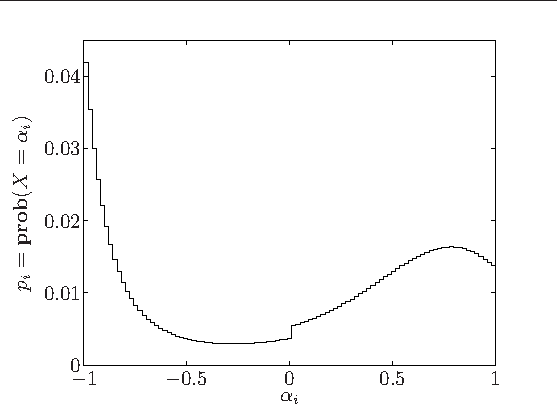
\includegraphics[width=.70\textwidth]{figures/ch07-figure-2.pdf}
\caption*{图7.2\quad 满足约束（7.8）的最大熵分布。}
\end{figure}
结果见图7.3，上、下两条曲线分别为上、下界，中间曲线为最大熵分布的累计分布。
\end{origexample}

\begin{origexample}{7.3}
\textbf{边缘分布已知时风险概率的界。}设随机变量 $X$、$Y$ 表示两项投资的收益。假设 $X$ 取值于 $\{\alpha_1,\ldots,\alpha_n\}\subseteq\R$，$Y$ 取值于 $\{\beta_1,\ldots,\beta_m\}\subseteq\R$，且 $p_{ij}=\Prob(X=\alpha_i,Y=\beta_j)$。两项收益的边缘分布已知，即
\begin{equation}
 \sum_{j=1}^mp_{ij}=r_i,\quad i=1,\ldots,n,\qquad
 \sum_{i=1}^np_{ij}=q_j,\quad j=1,\ldots,m,\tag{7.9}
\end{equation}
但除此以外，对联合分布 $p$ 一无所知。这定义了与给定边缘分布一致的联合分布多面体。

现在同时作这两项投资，总收益为随机变量 $X+Y$。我们希望计算某个损失水平或低收益水平的概率上界，即 $\Prob(X+Y<\gamma)$。求解线性规划
\[
\begin{array}{ll}
\text{最大化}&\sum\{p_{ij}\mid\alpha_i+\beta_j<\gamma\}\\
\text{满足}&\text{（7.9）},\quad p_{ij}\ge0,\quad i=1,\ldots,n,\quad j=1,\ldots,m
\end{array}
\]
可得该概率的紧上界。其最优值是最大的损失概率，最优解 $p^\star$ 是与给定边缘分布一致、且使损失概率最大的联合分布。

同样方法也可用于这两项投资的衍生品。设衍生品收益为 $R(X,Y)$，其中 $R:\R^2\to\R$。

% Source PDF page 378 (printed p. 364)
\begin{figure}[htbp]\centering
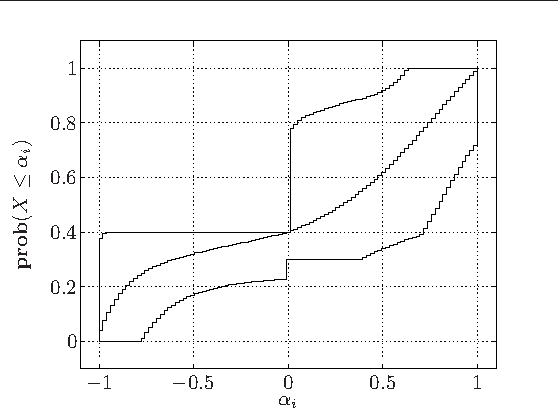
\includegraphics[width=.70\textwidth]{figures/ch07-figure-3.pdf}
\caption*{图7.3\quad 最上方与最下方曲线，表示在所有满足（7.8）的分布中，累计分布函数 $\Prob(X\le\alpha_i)$ 可能达到的最大值与最小值。中间曲线为满足（7.8）的最大熵分布的累计分布。}
\end{figure}
通过求解类似线性规划，对目标函数
\[
 \sum\{p_{ij}\mid R(\alpha_i,\beta_j)<\gamma\}
\]
分别最小化与最大化，就能计算 $\Prob(R<\gamma)$ 的精确下界与上界。
\end{origexample}

\section{最优检测器设计与假设检验}
设随机变量 $X$ 取值于 $\{1,\ldots,n\}$，其分布依赖参数 $\theta\in\{1,\ldots,m\}$。$\theta$ 的 $m$ 种可能取值对应的 $X$ 分布，可用矩阵 $P\in\R^{n\times m}$ 表示，其元素为
\[
 p_{kj}=\Prob(X=k\mid\theta=j).
\]
$P$ 的第 $j$ 列为参数值 $\theta=j$ 对应的概率分布。

考虑根据观测到的一个 $X$ 样本估计 $\theta$。换言之，样本 $X$ 由 $m$ 种可能分布中的一种产生，我们要猜测是哪一种。$\theta$ 的 $m$ 个值称为\emph{假设}，猜测哪个假设正确，即哪个分布生成观测样本 $X$，称为\emph{假设检验}。许多情况下，一个假设对应正常情况，其余各假设分别对应某种异常事件。此时，假设检验可解释为：观测 $X$ 的一个值，然后判断是否发生异常；若发生，又是哪种异常。因此，假设检验也称为\emph{检测}。

% Source PDF page 379 (printed p. 365)
大多数情况下，假设的顺序没有意义，只是任意标记为 $\theta=1,\ldots,m$ 的 $m$ 个不同假设。如果 $\widehat\theta=\theta$，其中 $\widehat\theta$ 是对 $\theta$ 的估计，就正确猜中了参数 $\theta$；如果 $\widehat\theta\ne\theta$，则猜测错误，把 $\widehat\theta$ 误作了 $\theta$。另一些情况下，假设的顺序有意义，这时 $\widehat\theta>\theta$，即高估 $\theta$，就是有意义的事件。

也可以将 $\theta$ 参数化为不属于 $\{1,\ldots,m\}$ 的其他值，例如 $\theta\in\{\theta_1,\ldots,\theta_m\}$，其中 $\theta_i$ 互异。这些值可以是实数，也可以是向量，例如用于指定第 $k$ 个分布的均值与方差。此时，参数估计误差的范数 $\norm{\widehat\theta-\theta}$ 就有意义。

\subsection{确定性检测器与随机化检测器}
确定性\emph{估计器}或\emph{检测器}，是从可能观测值集合 $\{1,\ldots,n\}$ 到假设集合 $\{1,\ldots,m\}$ 的函数 $\psi$。若观测到 $X=k$，就将 $\theta$ 猜为 $\widehat\theta=\psi(k)$。一种显然的确定性检测器是\emph{最大似然检测器}：
\begin{equation}
 \widehat\theta=\psi_{\mathrm{ml}}(k)=\argmax_jp_{kj}.\tag{7.10}
\end{equation}
观测到 $X=k$ 后，$\theta$ 的最大似然估计，就是在可能分布中使观测 $X=k$ 的概率最大的参数值。

我们考虑确定性检测器的一种推广：给定 $X$ 的观测值后，$\theta$ 的估计为随机的。$\theta$ 的\emph{随机化检测器}是一个随机变量 $\widehat\theta\in\{1,\ldots,m\}$，其分布依赖于 $X$ 的观测值。它可由矩阵 $T\in\R^{m\times n}$ 定义，元素为
\[
 t_{ik}=\Prob(\widehat\theta=i\mid X=k).
\]
其含义是：观测到 $X=k$ 时，检测器以概率 $t_{ik}$ 输出 $\widehat\theta=i$。将 $T$ 的第 $k$ 列记为 $t_k$，它给出观测 $X=k$ 时 $\widehat\theta$ 的分布。若 $T$ 每一列都是单位向量，则随机化检测器就是确定性检测器，即 $\widehat\theta$ 是 $X$ 观测值的确定性函数。

乍看起来，在估计或检测过程中故意加入额外随机性，似乎只会使估计器变差。但下面将看到，某些例子中随机化检测器优于所有确定性估计器。

我们关心如何设计定义随机化检测器的矩阵 $T$。显然，$T$ 的各列 $t_k$ 必须满足线性等式与不等式约束
\begin{equation}
 t_k\succeq0,\qquad\one^{\T}t_k=1.\tag{7.11}
\end{equation}

% Source PDF page 380 (printed p. 366)
\subsection{检测概率矩阵}
对矩阵 $T$ 定义的随机化检测器，定义\emph{检测概率矩阵} $D=TP$。有
\[
 D_{ij}=(TP)_{ij}=\Prob(\widehat\theta=i\mid\theta=j),
\]
所以 $D_{ij}$ 表示实际上 $\theta=j$ 时，猜为 $\widehat\theta=i$ 的概率。$m\times m$ 检测概率矩阵 $D$ 刻画了 $T$ 所定义随机化检测器的性能。对角元 $D_{ii}$ 表示 $\theta=i$ 时猜为 $\widehat\theta=i$ 的概率，即正确检测到 $\theta=i$ 的概率。非对角元 $D_{ij}$（$i\ne j$）是将 $\theta=i$ 误作 $\theta=j$ 的概率，也就是实际上 $\theta=j$ 时猜为 $\widehat\theta=i$ 的概率。如果 $D=I$，检测器就是完美的：不论参数 $\theta$ 是什么，都能正确猜为 $\widehat\theta=\theta$。

将 $D$ 的对角元排列成向量，称为\emph{检测概率}，记为 $P^d$：
\[
 P_i^d=D_{ii}=\Prob(\widehat\theta=i\mid\theta=i).
\]
\emph{错误概率}是其补，记为 $P^e$：
\[
 P_i^e=1-D_{ii}=\Prob(\widehat\theta\ne i\mid\theta=i).
\]
由于 $D$ 各列元素之和为一，错误概率也可表示为
\[
 P_i^e=\sum_{j\ne i}D_{ji}.
\]

\subsection{最优检测器设计}
本节说明，检测器设计中的许多目标都是 $D$ 的线性函数、仿射函数或凸分段线性函数，因此也是优化变量 $T$ 的这类函数。类似地，许多约束可用 $D$ 的线性不等式表示。所以，多种最优检测器设计问题都可写成线性规划。第7.3.4节将看到，其中一些问题具有简单解；本节只进行建模。

\subsubsection*{错误与检测概率的限制}
可对正确检测第 $j$ 个假设的概率施加下界：
\[
 P_j^d=D_{jj}\ge L_j,
\]
它是 $D$，从而也是 $T$ 的线性不等式。类似地，可对将 $\theta=i$ 误作 $\theta=j$ 的概率施加上界：
\[
 D_{ij}\le U_{ij}.
\]

% Source PDF page 381 (printed p. 367)
这些同样是 $T$ 的线性约束。任意一个检测概率都可作为待最大化的目标，任意一个错误概率都可作为待最小化的目标。

\subsubsection*{极小极大检测器设计}
可将极小极大错误概率 $\max_jP_j^e$ 作为待最小化目标，它是 $D$，从而也是 $T$ 的分段线性凸函数。只考虑这一目标，得到最小化最大检测错误概率的问题：
\[
\begin{array}{ll}
\text{最小化}&\max_jP_j^e\\
\text{满足}&t_k\succeq0,\quad\one^{\T}t_k=1,\quad k=1,\ldots,n,
\end{array}
\]
变量为 $t_1,\ldots,t_n\in\R^m$。该问题可重写为线性规划。极小极大检测器使 $m$ 个假设中最坏，即最大的错误概率最小。

当然，还可在极小极大检测器设计中加入其他约束。

\subsubsection*{Bayes检测器设计}
Bayes检测器设计给定假设的先验分布 $q\in\R^m$，其中
\[
 q_i=\Prob(\theta=i).
\]
此时，$p_{ij}$ 解释为给定 $\theta$ 时 $X$ 的条件概率。检测器的错误概率为 $q^{\T}P^e$，是 $T$ 的仿射函数。Bayes最优检测器是线性规划
\[
\begin{array}{ll}
\text{最小化}&q^{\T}P^e\\
\text{满足}&t_k\succeq0,\quad\one^{\T}t_k=1,\quad k=1,\ldots,n
\end{array}
\]
的解。第7.3.4节将看到，该问题有简单解析解。

一个特殊情形是 $q=(1/m)\one$，此时Bayes最优检测器最小化各假设的无权平均错误概率。第7.3.4节将说明，最大似然检测器（7.10）对这个问题最优。

\subsubsection*{偏差、均方误差及其他量}
这里假设 $\theta$ 的取值顺序有意义，即当 $i>j$ 时，$\theta=i$ 可理解为比 $\theta=j$ 更大的参数值。例如，若 $\theta=i$ 对应已经发生 $i$ 个事件的假设，就是这种情形。这时可能关心
\[
 \Prob(\widehat\theta>\theta\mid\theta=i),
\]
即 $\theta=i$ 时高估 $\theta$ 的概率。它是 $D$ 的仿射函数：
\[
 \Prob(\widehat\theta>\theta\mid\theta=i)=\sum_{j>i}D_{ji}.
\]

% Source PDF page 382 (printed p. 368)
所以该概率的上限可表示为 $D$，从而也是 $T$ 的线性不等式。再例如，当 $\theta=i$ 时，误判超过一的概率
\[
 \Prob(\abs{\widehat\theta-\theta}>1\mid\theta=i)
 =\sum_{\abs{j-i}>1}D_{ji}
\]
也是 $D$ 的线性函数。

现在设参数取值为 $\{\theta_1,\ldots,\theta_m\}\subseteq\R$。估计或检测的参数误差为 $\widehat\theta-\theta$，若干关心的量都可用 $D$ 的线性函数表示。例如：
\begin{itemize}
\item \emph{偏差。}$\theta=\theta_i$ 时，检测器偏差为线性函数
\[
 \E_i(\widehat\theta-\theta)=\sum_{j=1}^m(\theta_j-\theta_i)D_{ji},
\]
其中 $\E$ 的下标表示，期望是相对于假设 $\theta=\theta_i$ 下的分布计算的。
\item \emph{均方误差。}$\theta=\theta_i$ 时，检测器均方误差为线性函数
\[
 \E_i(\widehat\theta-\theta)^2=\sum_{j=1}^m(\theta_j-\theta_i)^2D_{ji}.
\]
\item \emph{平均绝对误差。}$\theta=\theta_i$ 时，检测器平均绝对误差为线性函数
\[
 \E_i\abs{\widehat\theta-\theta}=\sum_{j=1}^m\abs{\theta_j-\theta_i}D_{ji}.
\]
\end{itemize}

\subsection{多准则形式与标量化}
最优检测器设计可以看作多准则问题，约束为（7.11），$m(m-1)$ 个目标为 $D$ 的非对角元，即不同类型检测错误的概率：
\begin{equation}
\begin{array}{ll}
\text{最小化（关于 }\R_+^{m(m-1)}\text{）}&D_{ij},\quad i,j=1,\ldots,m,\quad i\ne j\\
\text{满足}&t_k\succeq0,\quad\one^{\T}t_k=1,\quad k=1,\ldots,n,
\end{array}\tag{7.12}
\end{equation}
变量为 $t_1,\ldots,t_n\in\R^m$。由于每个目标 $D_{ij}$ 都是变量的线性函数，这是多准则线性规划。

取加权和目标
\[
 \sum_{i,j=1}^mW_{ij}D_{ij}=\tr(W^{\T}D),
\]
可以将其标量化。

% Source PDF page 383 (printed p. 369)
权重矩阵 $W\in\R^{m\times m}$ 满足
\[
 W_{ii}=0,\quad i=1,\ldots,m,\qquad
 W_{ij}>0,\quad i,j=1,\ldots,m,\quad i\ne j.
\]
该目标是 $m(m-1)$ 个错误概率的加权和，$W_{ij}$ 对应实际为 $\theta=j$、却猜为 $\widehat\theta=i$ 的错误。权重矩阵有时称为\emph{损失矩阵}。

为找到多准则问题（7.12）的Pareto最优点，建立标量优化问题
\begin{equation}
\begin{array}{ll}
\text{最小化}&\tr(W^{\T}D)\\
\text{满足}&t_k\succeq0,\quad\one^{\T}t_k=1,\quad k=1,\ldots,n,
\end{array}\tag{7.13}
\end{equation}
它是线性规划，且关于 $t_1,\ldots,t_n$ 可分。目标可写成各 $t_k$ 的线性函数之和：
\[
 \tr(W^{\T}D)=\tr(W^{\T}TP)=\tr(PW^{\T}T)
 =\sum_{k=1}^nc_k^{\T}t_k,
\]
其中 $c_k$ 是 $WP^{\T}$ 的第 $k$ 列。约束也可分，即各 $t_i$ 分别有自己的约束。因此，可以分别求解 $k=1,\ldots,n$ 时的问题
\[
\begin{array}{ll}
\text{最小化}&c_k^{\T}t_k\\
\text{满足}&t_k\succeq0,\quad\one^{\T}t_k=1,
\end{array}
\]
从而求解（7.13）。每个问题都有简单解析解，见习题4.8。先找到索引 $q$，使 $c_{kq}=\min_jc_{kj}$，再取 $t_k^\star=e_q$。这个最优点对应确定性检测器：当观测到 $X=k$ 时，估计为
\begin{equation}
 \widehat\theta=\argmin_j(WP^{\T})_{jk}.\tag{7.14}
\end{equation}
所以，对于非对角元均为正的每个权重矩阵 $W$，都能找到一个使加权和目标最小的确定性检测器。这似乎暗示无需随机化检测器，但下面会看到并非如此。多准则线性规划（7.12）的Pareto最优权衡面为分段线性的；（7.14）形式的确定性检测器，对应Pareto最优面上的顶点。

\subsubsection*{MAP与ML检测器}
考虑先验分布为 $q$ 的Bayes检测器设计。平均错误概率为
\[
 q^{\T}P^e=\sum_{j=1}^mq_j\sum_{i\ne j}D_{ij}
 =\sum_{i,j=1}^mW_{ij}D_{ij},
\]
其中权重矩阵定义为
\[
 W_{ij}=q_j,\quad i,j=1,\ldots,m,\quad i\ne j,\qquad
 W_{ii}=0,\quad i=1,\ldots,m.
\]

% Source PDF page 384 (printed p. 370)
因此，Bayes最优检测器由确定性检测器（7.14）给出，此时
\[
 (WP^{\T})_{jk}=\sum_{i\ne j}q_ip_{ki}
 =\sum_{i=1}^mq_ip_{ki}-q_jp_{kj}.
\]
第一项不依赖 $j$，所以观测到 $X=k$ 时，最优检测器就是
\[
 \widehat\theta=\argmax_j(p_{kj}q_j).
\]
这个解有简单解释：$p_{kj}q_j$ 是 $\theta=j$ 且 $X=k$ 的概率，因此该检测器为\emph{最大后验概率}（MAP）检测器。

特别地，若 $q=(1/m)\one$，即 $\theta$ 的先验分布均匀，该MAP检测器化为\emph{最大似然}（ML）检测器：
\[
 \widehat\theta=\argmax_jp_{kj}.
\]
所以，最大似然检测器最小化无权平均错误概率。

\subsection{二元假设检验}
作为说明，考虑 $m=2$ 的特殊情形，称为\emph{二元假设检验}。随机变量 $X$ 由两个分布中的一个产生，为简化记号，将两个分布记为 $p\in\R^n$、$q\in\R^n$。通常，$\theta=1$ 对应正常情况，$\theta=2$ 对应要检测的某种异常事件。若 $\widehat\theta=1$，称检验为\emph{阴性}，即猜测事件未发生；若 $\widehat\theta=2$，称为\emph{阳性}，即猜测事件已发生。

检测概率矩阵 $D\in\R^{2\times2}$ 通常写成
\[
 D=\begin{bmatrix}1-P_{\mathrm{fp}}&P_{\mathrm{fn}}\\
 P_{\mathrm{fp}}&1-P_{\mathrm{fn}}\end{bmatrix}.
\]
$P_{\mathrm{fn}}$ 是\emph{假阴性}概率，即事件实际发生但检验为阴性；$P_{\mathrm{fp}}$ 是\emph{假阳性}概率，即事件实际未发生但检验为阳性，也称为\emph{虚警概率}。最优检测器设计是以 $P_{\mathrm{fn}}$、$P_{\mathrm{fp}}$ 为目标的双准则问题。

两者的最优权衡曲线称为\emph{接收者工作特征}（ROC），由分布 $p,q$ 确定。按照第7.3.4节对双准则问题进行标量化，便可求出ROC。给定权重矩阵 $W$，最优检测器（7.14）为
\[
 \widehat\theta=\begin{cases}
 1&W_{21}p_k>W_{12}q_k,\\
 2&W_{21}p_k\le W_{12}q_k.
 \end{cases}
\]

% Source PDF page 385 (printed p. 371)
\begin{figure}[htbp]\centering
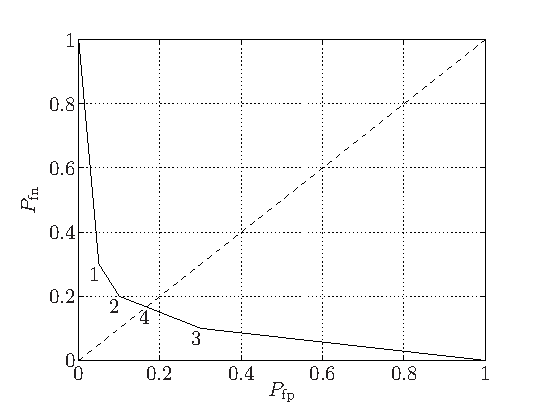
\includegraphics[width=.72\textwidth]{figures/ch07-figure-4.pdf}
\caption*{图7.4\quad 对（7.15）中的矩阵 $P$，假阴性概率与假阳性概率的最优权衡曲线。标为1至3的顶点对应确定性检测器；标为4的点对应随机化的极小极大检测器。虚线为 $P_{\mathrm{fn}}=P_{\mathrm{fp}}$，即两种错误概率相等的点。}
\end{figure}
上式是观测到 $X=k$ 时的判决。这称为\emph{似然比门限检验}：如果比值 $p_k/q_k$ 超过门限 $W_{12}/W_{21}$，检验为阴性，即 $\widehat\theta=1$；否则为阳性。选择不同门限，会得到假阳性与假阴性错误概率不同的确定性Pareto最优检测器。该结果称为\emph{Neyman--Pearson引理}。

似然比检测器并未给出全部Pareto最优检测器；它们是分段线性最优权衡曲线上的顶点。

\begin{origexample}{7.4}
考虑 $n=4$ 的二元假设检验例子，
\begin{equation}
 P=\begin{bmatrix}
 0.70&0.10\\0.20&0.10\\0.05&0.70\\0.05&0.10
 \end{bmatrix}.\tag{7.15}
\end{equation}
$P_{\mathrm{fn}}$ 与 $P_{\mathrm{fp}}$ 的最优权衡曲线，即接收者工作特征曲线，见图7.4。左端点对应始终输出阴性、与 $X$ 观测值无关的检测器；右端点对应始终输出阳性的检测器。标为1、2、3的顶点，分别对应确定性检测器
\[
 T^{(1)}=\begin{bmatrix}1&1&0&1\\0&0&1&0\end{bmatrix},\qquad
 T^{(2)}=\begin{bmatrix}1&1&0&0\\0&0&1&1\end{bmatrix},
\]

% Source PDF page 386 (printed p. 372)
\[
 T^{(3)}=\begin{bmatrix}1&0&0&0\\0&1&1&1\end{bmatrix}.
\]
标为4的点对应非确定性检测器
\[
 T^{(4)}=\begin{bmatrix}1&2/3&0&0\\0&1/3&1&1\end{bmatrix},
\]
它是极小极大检测器，假阳性与假阴性的概率相等，本例中均为 $1/6$。每个确定性检测器至少有一种错误概率超过 $1/6$，因此这是随机化检测器优于所有确定性检测器的例子。
\end{origexample}

\subsection{稳健检测器}
到目前为止，假设给出每个参数 $\theta$ 下观测变量 $X$ 分布的矩阵 $P$ 已知。本节考虑这些分布未知、但给定某些先验信息的情形。设 $P\in\mathcal P$，其中 $\mathcal P$ 为可能分布的集合。对由 $T$ 刻画的随机化检测器，检测概率矩阵 $D$ 现在依赖于具体的 $P$。我们按 $P\in\mathcal P$ 中的最坏值评价错误概率。定义\emph{最坏情形检测概率矩阵} $D^{\mathrm{wc}}$ 为
\[
 D_{ij}^{\mathrm{wc}}=\sup_{P\in\mathcal P}D_{ij},\qquad
 i,j=1,\ldots,m,\quad i\ne j,
\]
以及
\[
 D_{ii}^{\mathrm{wc}}=\inf_{P\in\mathcal P}D_{ii},\qquad i=1,\ldots,m.
\]
非对角元给出 $P\in\mathcal P$ 中最大可能的错误概率，对角元给出最小可能的检测概率。注意，一般有 $\sum_{i=1}^nD_{ij}^{\mathrm{wc}}\ne1$，即最坏情形检测概率矩阵的各列和不一定等于一。

定义最坏情形错误概率为
\[
 P_i^{\mathrm{wce}}=1-D_{ii}^{\mathrm{wc}}.
\]
因此，$P_i^{\mathrm{wce}}$ 是 $\theta=i$ 时，在 $\mathcal P$ 所有可能分布中的最大错误概率。

用最坏情形检测概率矩阵，或最坏情形错误概率向量，可以构造多种稳健检测器设计问题。本节其余部分集中讨论稳健极小极大检测器，以此为代表说明这些思想。

定义\emph{稳健极小极大检测器}，使所有假设下的最坏错误概率最小，即最小化
\[
 \max_iP_i^{\mathrm{wce}}
 =\max_{i=1,\ldots,m}\sup_{P\in\mathcal P}(1-(TP)_{ii})
 =1-\min_{i=1,\ldots,m}\inf_{P\in\mathcal P}(TP)_{ii}.
\]
稳健极小极大检测器最小化所有 $m$ 个假设、所有 $P\in\mathcal P$ 中最坏的错误概率。

% Source PDF page 387 (printed p. 373)
\subsubsection*{有限 $\mathcal P$ 的稳健极小极大检测器}
可能分布集合有限时，稳健极小极大检测器设计很容易写成线性规划。设 $\mathcal P=\{P_1,\ldots,P_k\}$，可求解
\[
\begin{array}{ll}
\text{最大化}&\displaystyle\min_{i=1,\ldots,m}\inf_{P\in\mathcal P}(TP)_{ii}
 =\min_{i=1,\ldots,m}\min_{j=1,\ldots,k}(TP_j)_{ii}\\
\text{满足}&t_i\succeq0,\quad\one^{\T}t_i=1,\quad i=1,\ldots,n
\end{array}
\]
得到稳健极小极大检测器。目标为分段线性凹函数，因此问题可表示为线性规划。也可以将可能分布集取为多面体 $\conv\mathcal P$，相应最坏情形检测矩阵和稳健极小极大检测器都不变。

\subsubsection*{多面体 $\mathcal P$ 的稳健极小极大检测器}
当 $\mathcal P$ 是由线性等式与不等式描述的多面体时，也能高效地将稳健极小极大检测器问题写成线性规划。这一形式较不直观，要依靠 $\mathcal P$ 的对偶表示。

为简化讨论，假设 $\mathcal P$ 具有形式
\begin{equation}
 \mathcal P=\left\{P=\begin{bmatrix}p_1&\cdots&p_m\end{bmatrix}
 \ \middle|\ A_kp_k=b_k,\ \one^{\T}p_k=1,\ p_k\succeq0\right\}.\tag{7.16}
\end{equation}
换言之，对每个分布 $p_k$，给定某些期望值 $A_kp_k=b_k$，它们可以是已知的矩、概率等。推广到给定期望不等式的情形很直接。

稳健极小极大设计问题为
\[
\begin{array}{ll}
\text{最大化}&\gamma\\
\text{满足}&\inf\{\widetilde t_i^{\T}p\mid A_ip=b_i,\ \one^{\T}p=1,\ p\succeq0\}\ge\gamma,
 \quad i=1,\ldots,m,\\
&t_i\succeq0,\quad\one^{\T}t_i=1,\quad i=1,\ldots,n,
\end{array}
\]
其中 $\widetilde t_i^{\T}$ 表示 $T$ 的第 $i$ 行，因此 $(TP)_{ii}=\widetilde t_i^{\T}p_i$。由线性规划对偶性，
\[
\begin{aligned}
 &\inf\{\widetilde t_i^{\T}p\mid A_ip=b_i,\ \one^{\T}p=1,\ p\succeq0\}\\
 &\qquad=\sup\{\nu^{\T}b_i+\mu\mid A_i^{\T}\nu+\mu\one\preceq\widetilde t_i\}.
\end{aligned}
\]
据此，稳健极小极大检测器设计可表示为线性规划
\[
\begin{array}{ll}
\text{最大化}&\gamma\\
\text{满足}&\nu_i^{\T}b_i+\mu_i\ge\gamma,\quad i=1,\ldots,m,\\
&A_i^{\T}\nu_i+\mu_i\one\preceq\widetilde t_i,\quad i=1,\ldots,m,\\
&t_i\succeq0,\quad\one^{\T}t_i=1,\quad i=1,\ldots,n,
\end{array}
\]
变量为 $\nu_1,\ldots,\nu_m$、$\mu_1,\ldots,\mu_n$ 及 $T$，后者的列为 $t_i$，行为 $\widetilde t_i^{\T}$。

\begin{origexample}{7.5}
\textbf{稳健二元假设检验。}设 $m=2$，且（7.16）中的 $\mathcal P$ 由下列数据定义：
\[
 A_1=A_2=A=\begin{bmatrix}a_1&a_2&\cdots&a_n\\
 a_1^2&a_2^2&\cdots&a_n^2\end{bmatrix},\qquad
 b_1=\begin{bmatrix}\alpha_1\\\alpha_2\end{bmatrix},\qquad
 b_2=\begin{bmatrix}\beta_1\\\beta_2\end{bmatrix}.
\]
对这个 $\mathcal P$ 设计稳健极小极大检测器，可以解释为二元假设检验问题：根据随机变量 $X\in\{a_1,\ldots,a_n\}$ 的一次观测，在以下两个假设中选择：

% Source PDF page 388 (printed p. 374)
\begin{enumerate}
\item $\E X=\alpha_1$、$\E X^2=\alpha_2$；
\item $\E X=\beta_1$、$\E X^2=\beta_2$。
\end{enumerate}
令 $\widetilde t^{\T}$ 为 $T$ 的第一行，则 $(\one-\widetilde t)^{\T}$ 为第二行。给定 $\widetilde t$，最坏情形的正确检测概率为
\[
\begin{aligned}
 D_{11}^{\mathrm{wc}}
 &=\inf\left\{\widetilde t^{\T}p\ \middle|\
 \sum_{i=1}^na_ip_i=\alpha_1,\ \sum_{i=1}^na_i^2p_i=\alpha_2,
 \ \one^{\T}p=1,\ p\succeq0\right\},\\
 D_{22}^{\mathrm{wc}}
 &=\inf\left\{(\one-\widetilde t)^{\T}p\ \middle|\
 \sum_{i=1}^na_ip_i=\beta_1,\ \sum_{i=1}^na_i^2p_i=\beta_2,
 \ \one^{\T}p=1,\ p\succeq0\right\}.
\end{aligned}
\]
利用线性规划对偶性，$D_{11}^{\mathrm{wc}}$ 可表示为线性规划
\[
\begin{array}{ll}
\text{最大化}&z_0+z_1\alpha_1+z_2\alpha_2\\
\text{满足}&z_0+a_iz_1+a_i^2z_2\le\widetilde t_i,\quad i=1,\ldots,n
\end{array}
\]
的最优值，变量为 $z_0,z_1,z_2\in\R$。类似地，$D_{22}^{\mathrm{wc}}$ 是线性规划
\[
\begin{array}{ll}
\text{最大化}&w_0+w_1\beta_1+w_2\beta_2\\
\text{满足}&w_0+a_iw_1+a_i^2w_2\le1-\widetilde t_i,\quad i=1,\ldots,n
\end{array}
\]
的最优值，变量为 $w_0,w_1,w_2\in\R$。为得到极小极大检测器，要最大化 $D_{11}^{\mathrm{wc}}$ 与 $D_{22}^{\mathrm{wc}}$ 的最小值，即求解
\[
\begin{array}{ll}
\text{最大化}&\gamma\\
\text{满足}&z_0+z_1\alpha_2+z_2\alpha_2\ge\gamma,\\
&w_0+\beta_1w_1+\beta_2w_2\ge\gamma,\\
&z_0+z_1a_i+z_2a_i^2\le\widetilde t_i,\quad i=1,\ldots,n,\\
&w_0+w_1a_i+w_2a_i^2\le1-\widetilde t_i,\quad i=1,\ldots,n,\\
&0\preceq\widetilde t\preceq\one.
\end{array}
\]
变量为 $z_0,z_1,z_2,w_0,w_1,w_2$ 和 $\widetilde t$。
\end{origexample}

\section{Chebyshev界与Chernoff界}
本节考虑两类经典的集合概率界，并说明它们的推广形式都能写成凸优化问题。原来的经典界对应具有解析解的简单凸优化问题；更一般情形的凸优化形式，可以计算更好的界，或者处理更复杂的情形。

\subsection{Chebyshev界}
Chebyshev界根据某些函数的已知期望，例如均值与方差，给出某个集合的概率上界。最简单的例子是Markov不等式：若 $X$ 是 $\R_+$ 上的随机变量，$\E X=\mu$，则无论 $X$ 的分布如何，都有 $\Prob(X\ge1)\le\mu$。

% Source PDF page 389 (printed p. 375)
另一个简单例子是Chebyshev界：若 $X$ 是 $\R$ 上的随机变量，$\E X=\mu$，$\E(X-\mu)^2=\sigma^2$，则无论分布如何，都有 $\Prob(\abs{X-\mu}\ge1)\le\sigma^2$。这些简单界背后的思想，可以推广为用凸优化计算概率界。

设 $X$ 是 $S\subseteq\R^m$ 上的随机变量，$C\subseteq S$ 是我们希望对其概率 $\Prob(X\in C)$ 求界的集合。用 $\one_C$ 表示 $C$ 的0--1指示函数，即 $z\in C$ 时 $\one_C(z)=1$，$z\notin C$ 时 $\one_C(z)=0$。

关于分布的先验知识，是一些函数的已知期望：
\[
 \E f_i(X)=a_i,\qquad i=1,\ldots,n,
\]
其中 $f_i:\R^m\to\R$。令 $f_0$ 为值恒等于一的常函数，总有 $\E f_0(X)=a_0=1$。考虑这些函数的线性组合
\[
 f(z)=\sum_{i=0}^nx_if_i(z),
\]
其中 $x_i\in\R$，$i=0,\ldots,n$。由已知的 $\E f_i(X)$，可得 $\E f(X)=a^{\T}x$。

假设 $f$ 满足对所有 $z\in S$ 有 $f(z)\ge\one_C(z)$，即在 $S$ 上逐点不小于 $C$ 的指示函数，则
\[
 \E f(X)=a^{\T}x\ge\E\one_C(X)=\Prob(X\in C).
\]
换言之，$a^{\T}x$ 是 $\Prob(X\in C)$ 的上界，对所有支撑于 $S$、满足 $\E f_i(X)=a_i$ 的分布都有效。

通过求解
\begin{equation}
\begin{array}{ll}
\text{最小化}&x_0+a_1x_1+\cdots+a_nx_n\\
\text{满足}&f(z)=\sum_{i=0}^nx_if_i(z)\ge1,\quad z\in C,\\
&f(z)=\sum_{i=0}^nx_if_i(z)\ge0,\quad z\in S,\ z\notin C,
\end{array}\tag{7.17}
\end{equation}
可寻找这类上界中最好的一个，变量为 $x\in\R^{n+1}$。该问题总凸，因为约束可表示为
\[
 g_1(x)=1-\inf_{z\in C}f(z)\le0,\qquad
 g_2(x)=-\inf_{z\in S\setminus C}f(z)\le0,
\]
其中 $g_1,g_2$ 凸。问题（7.17）也可视为\emph{半无限线性规划}：目标线性，包含无穷多个线性不等式，每个 $z\in S$ 对应一个。

简单情形下，（7.17）可解析求解。例如，取 $S=\R_+$、$C=[1,\infty)$、$f_0(z)=1$、$f_1(z)=z$，先验信息为 $\E f_1(X)=\E X=\mu\le1$。条件 $f(z)\ge0$ 对所有 $z\in S$ 成立，化为 $x_0\ge0$、$x_1\ge0$。条件 $f(z)\ge1$ 对所有 $z\in C$ 成立，即 $x_0+x_1z\ge1$ 对所有 $z\ge1$ 成立，化为 $x_0+x_1\ge1$。因此（7.17）成为
\[
\begin{array}{ll}
\text{最小化}&x_0+\mu x_1\\
\text{满足}&x_0\ge0,\quad x_1\ge0,\\
&x_0+x_1\ge1.
\end{array}
\]

% Source PDF page 390 (printed p. 376)
由于 $0\le\mu\le1$，这个简单线性规划的最优点为 $x_0=0$、$x_1=1$，得到经典Markov界 $\Prob(X\ge1)\le\mu$。其他情况下，可以用凸优化求解（7.17）。

\begin{quote}\textbf{说明7.1\quad 对偶性与Chebyshev界问题。}
Chebyshev界问题（7.17）给出对所有满足指定期望约束的概率测度都成立的 $\Prob(X\in C)$ 上界。因此，可将（7.17）看作对以下无限维问题的最优值求界：
\begin{equation}
\begin{array}{ll}
\text{最大化}&\displaystyle\int_C\pi(\mathrm dz)\\
\text{满足}&\displaystyle\int_S f_i(z)\pi(\mathrm dz)=a_i,\quad i=1,\ldots,n,\\
&\displaystyle\int_S\pi(\mathrm dz)=1,\\
&\pi\ge0,
\end{array}\tag{7.18}
\end{equation}
变量为测度 $\pi$，$\pi\ge0$ 表示它是非负测度。

Chebyshev问题（7.17）为（7.18）求界，因此两者由对偶性联系起来并不意外。虽然半无限与无限维问题超出本书范围，我们仍可形式地构造（7.17）的对偶：引入拉格朗日乘子函数 $p:S\to\R$，其中 $p(z)$ 是不等式 $f(z)\ge1$（$z\in C$）或 $f(z)\ge0$（$z\in S\setminus C$）的乘子。将有限维中的求和改为对 $z$ 积分，得到形式对偶
\[
\begin{array}{ll}
\text{最大化}&\displaystyle\int_Cp(z)\,\mathrm dz\\
\text{满足}&\displaystyle\int_Sf_i(z)p(z)\,\mathrm dz=a_i,\quad i=1,\ldots,n,\\
&\displaystyle\int_Sp(z)\,\mathrm dz=1,\\
&p(z)\ge0,\quad\text{对所有 }z\in S,
\end{array}
\]
优化变量为函数 $p$。这与（7.18）本质上相同。
\end{quote}

\subsubsection*{已知一阶与二阶矩时的概率界}
例如，设 $S=\R^m$，给定随机变量 $X$ 的一阶与二阶矩：
\[
 \E X=a\in\R^m,\qquad\E XX^{\T}=\Sigma\in\mathbf S^m.
\]
也就是说，已知 $m$ 个函数 $z_i$（$i=1,\ldots,m$）以及 $m(m+1)/2$ 个函数 $z_iz_j$（$i,j=1,\ldots,m$）的期望，但没有分布的其他信息。

这时可将 $f$ 写成一般二次函数
\[
 f(z)=z^{\T}Pz+2q^{\T}z+r,
\]
变量，也就是前面讨论中的向量 $x$，为 $P\in\mathbf S^m$、$q\in\R^m$、$r\in\R$。利用已知的一阶与二阶矩，有
\[
\begin{aligned}
 \E f(X)&=\E(X^{\T}PX+2q^{\T}X+r)\\
 &=\E\tr(PXX^{\T})+2\E q^{\T}X+r\\
 &=\tr(\Sigma P)+2q^{\T}a+r.
\end{aligned}
\]

% Source PDF page 391 (printed p. 377)
$f(z)\ge0$ 对所有 $z$ 成立，可表示为线性矩阵不等式
\[
 \begin{bmatrix}P&q\\q^{\T}&r\end{bmatrix}\succeq0.
\]
特别地，$P\succeq0$。

现设 $C$ 是一个开多面体的补集，
\[
 C=\R^m\setminus\mathcal P,\qquad
 \mathcal P=\{z\mid a_i^{\T}z<b_i,\ i=1,\ldots,k\}.
\]
对所有 $z\in C$ 要求 $f(z)\ge1$，等价于对 $i=1,\ldots,k$ 要求
\[
 a_i^{\T}z\ge b_i\quad\Longrightarrow\quad z^{\T}Pz+2q^{\T}z+r\ge1.
\]
这又可表示为：存在 $\tau_1,\ldots,\tau_k\ge0$，使
\[
 \begin{bmatrix}P&q\\q^{\T}&r-1\end{bmatrix}
 \succeq\tau_i\begin{bmatrix}0&a_i/2\\a_i^{\T}/2&-b_i\end{bmatrix},
 \qquad i=1,\ldots,k,
\]
见第B.2节。

综合可得，Chebyshev界问题（7.17）可写为
\begin{equation}
\begin{array}{ll}
\text{最小化}&\tr(\Sigma P)+2q^{\T}a+r\\
\text{满足}&\displaystyle\begin{bmatrix}P&q\\q^{\T}&r-1\end{bmatrix}
 \succeq\tau_i\begin{bmatrix}0&a_i/2\\a_i^{\T}/2&-b_i\end{bmatrix},
 \quad i=1,\ldots,k,\\[3pt]
&\tau_i\ge0,\quad i=1,\ldots,k,\\[3pt]
&\displaystyle\begin{bmatrix}P&q\\q^{\T}&r\end{bmatrix}\succeq0.
\end{array}\tag{7.19}
\end{equation}
这是关于 $P,q,r,\tau_1,\ldots,\tau_k$ 的半正定规划。设最优值为 $\alpha$，它就是所有均值为 $a$、二阶矩为 $\Sigma$ 的分布下 $\Prob(X\in C)$ 的上界。反过来，$1-\alpha$ 是 $\Prob(X\in\mathcal P)$ 的下界。

\begin{quote}\textbf{说明7.2\quad 对偶性与Chebyshev界问题。}
与（7.19）对应的对偶半正定规划可写为
\[
\begin{array}{ll}
\text{最大化}&\sum_{i=1}^k\lambda_i\\
\text{满足}&a_i^{\T}z_i\ge b\lambda_i,\quad i=1,\ldots,k,\\[3pt]
&\displaystyle\sum_{i=1}^k\begin{bmatrix}Z_i&z_i\\z_i^{\T}&\lambda_i\end{bmatrix}
 \preceq\begin{bmatrix}\Sigma&a\\a^{\T}&1\end{bmatrix},\\[3pt]
&\displaystyle\begin{bmatrix}Z_i&z_i\\z_i^{\T}&\lambda_i\end{bmatrix}\succeq0,
 \quad i=1,\ldots,k.
\end{array}
\]
变量为 $Z_i\in\mathbf S^m$、$z_i\in\R^m$、$\lambda_i\in\R$，$i=1,\ldots,k$。由于（7.19）严格可行，强对偶成立，且对偶最优值可取到。

这个对偶问题有一个有趣的概率解释。设 $Z_i,z_i,\lambda_i$ 对偶可行，且 $\lambda$ 的前 $r$ 个分量为正，其余为零。

% Source PDF page 392 (printed p. 378)
为简单起见，还假设 $\sum_{i=1}^k\lambda_i<1$。定义
\[
\begin{aligned}
 x_i&=(1/\lambda_i)z_i,\quad i=1,\ldots,r,\\
 w_0&=\frac1\mu\left(a-\sum_{i=1}^r\lambda_ix_i\right),\\
 W&=\frac1\mu\left(\Sigma-\sum_{i=1}^r\lambda_ix_ix_i^{\T}\right),
\end{aligned}
\]
其中 $\mu=1-\sum_{i=1}^k\lambda_i$。用这些定义，对偶可行性约束可写为
\[
 a_i^{\T}x_i\ge b_i,\qquad i=1,\ldots,r,
\]
以及
\[
 \sum_{i=1}^r\lambda_i\begin{bmatrix}x_ix_i^{\T}&x_i\\x_i^{\T}&1\end{bmatrix}
 +\mu\begin{bmatrix}W&w_0\\w_0^{\T}&1\end{bmatrix}
 =\begin{bmatrix}\Sigma&a\\a^{\T}&1\end{bmatrix}.
\]
此外，由对偶可行性，
\[
\begin{aligned}
 \mu\begin{bmatrix}W&w_0\\w_0^{\T}&1\end{bmatrix}
 &=\begin{bmatrix}\Sigma&a\\a^{\T}&1\end{bmatrix}
   -\sum_{i=1}^r\lambda_i\begin{bmatrix}x_ix_i^{\T}&x_i\\x_i^{\T}&1\end{bmatrix}\\
 &=\begin{bmatrix}\Sigma&a\\a^{\T}&1\end{bmatrix}
   -\sum_{i=1}^r\begin{bmatrix}(1/\lambda_i)z_iz_i^{\T}&z_i\\z_i^{\T}&\lambda_i\end{bmatrix}\\
 &\succeq\begin{bmatrix}\Sigma&a\\a^{\T}&1\end{bmatrix}
   -\sum_{i=1}^r\begin{bmatrix}Z_i&z_i\\z_i^{\T}&\lambda_i\end{bmatrix}\\
 &\succeq0.
\end{aligned}
\]
因此，$W\succeq w_0w_0^{\T}$，可分解为 $W-w_0w_0^{\T}=\sum_{i=1}^sw_iw_i^{\T}$。考虑具有以下分布的离散随机变量 $X$。如果 $s\ge1$，取
\[
\begin{array}{lll}
 X=x_i&\text{概率为 }\lambda_i,&i=1,\ldots,r,\\
 X=w_0+\sqrt{s}\,w_i&\text{概率为 }\mu/(2s),&i=1,\ldots,s,\\
 X=w_0-\sqrt{s}\,w_i&\text{概率为 }\mu/(2s),&i=1,\ldots,s.
\end{array}
\]
如果 $s=0$，取
\[
\begin{array}{lll}
 X=x_i&\text{概率为 }\lambda_i,&i=1,\ldots,r,\\
 X=w_0&\text{概率为 }\mu.&
\end{array}
\]
容易验证，$\E X=a$、$\E XX^{\T}=\Sigma$，即分布满足给定矩。此外，由于 $x_i\in C$，
\[
 \Prob(X\in C)\ge\sum_{i=1}^r\lambda_i.
\]
特别地，将这个解释应用于对偶最优解，便可构造一个使（7.19）的Chebyshev界取等号的分布，说明这一情形的界是紧的。
\end{quote}

% Source PDF page 393 (printed p. 379)
\subsection{Chernoff界}
设 $X$ 是 $\R$ 上的随机变量。Chernoff界指出
\[
 \Prob(X\ge u)\le\inf_{\lambda\ge0}\E e^{\lambda(X-u)},
\]
可写为
\begin{equation}
 \log\Prob(X\ge u)\le\inf_{\lambda\ge0}\{-\lambda u+\log\E e^{\lambda X}\}.\tag{7.20}
\end{equation}
回顾第106页例3.41，右侧的 $\log\E e^{\lambda X}$ 称为分布的\emph{累积量生成函数}，它总凸，因此被最小化的函数凸。当累积量生成函数有解析表达式，且关于 $\lambda$ 的最小化能解析完成时，（7.20）尤其有用。

例如，若 $X$ 为零均值、单位方差的高斯变量，则累积量生成函数为
\[
 \log\E e^{\lambda X}=\lambda^2/2.
\]
当 $u\ge0$ 时，$-\lambda u+\lambda^2/2$ 在 $\lambda\ge0$ 上的下确界于 $\lambda=u$ 处取到，因此对 $u\ge0$，Chernoff界为
\[
 \Prob(X\ge u)\le e^{-u^2/2}.
\]
Chernoff界背后的思想可以推广，用凸优化计算 $\R^m$ 中某个集合的概率界。设 $C\subseteq\R^m$，与前面讨论Chebyshev界时一样，用 $\one_C$ 表示 $C$ 的0--1指示函数。我们要推导 $\Prob(X\in C)$ 的上界。原则上，可通过Monte Carlo模拟或数值积分计算该概率，但两者的计算任务都可能很艰巨，而且都不能给出有保证的界。

取 $\lambda\in\R^m$、$\mu\in\R$，考虑函数 $f:\R^m\to\R$：
\[
 f(z)=e^{\lambda^{\T}z+\mu}.
\]
与Chebyshev界的推导一样，若对所有 $z$ 都有 $f(z)\ge\one_C(z)$，则
\[
 \Prob(X\in C)=\E\one_C(X)\le\E f(X).
\]
显然，对所有 $z$ 有 $f(z)\ge0$；对 $z\in C$ 要求 $f(z)\ge1$，等价于 $\lambda^{\T}z+\mu\ge0$，即 $-\lambda^{\T}z\le\mu$。因此，如果 $-\lambda^{\T}z\le\mu$ 对所有 $z\in C$ 成立，则
\[
 \Prob(X\in C)\le\E\exp(\lambda^{\T}X+\mu),
\]
取对数得
\[
 \log\Prob(X\in C)\le\mu+\log\E\exp(\lambda^{\T}X).
\]

% Source PDF page 394 (printed p. 380)
由此得到Chernoff界的一般形式：
\[
\begin{aligned}
 \log\Prob(X\in C)
 &\le\inf\{\mu+\log\E\exp(\lambda^{\T}X)\mid
 -\lambda^{\T}z\le\mu,\ \text{对所有 }z\in C\}\\
 &=\inf_\lambda\left\{\sup_{z\in C}(-\lambda^{\T}z)
       +\log\E\exp(\lambda^{\T}X)\right\}\\
 &=\inf_\lambda\left\{S_C(-\lambda)+\log\E\exp(\lambda^{\T}X)\right\},
\end{aligned}
\]
其中 $S_C$ 为 $C$ 的支撑函数。第二项 $\log\E\exp(\lambda^{\T}X)$ 是分布的累积量生成函数，总是凸的，见第106页例3.41。一般而言，计算这个界是凸优化问题。

\subsubsection*{高斯变量落在多面体内的Chernoff界}
作为具体例子，设 $X$ 为 $\R^m$ 上零均值、协方差为 $I$ 的高斯随机向量，累积量生成函数为
\[
 \log\E\exp(\lambda^{\T}X)=\lambda^{\T}\lambda/2.
\]
取非空多面体
\[
 C=\{x\mid Ax\preceq b\}.
\]
为用于Chernoff界，采用支撑函数 $S_C$ 的对偶刻画：
\[
\begin{aligned}
 S_C(y)&=\sup\{y^{\T}x\mid Ax\preceq b\}\\
 &=-\inf\{-y^{\T}x\mid Ax\preceq b\}\\
 &=-\sup\{-b^{\T}u\mid A^{\T}u=y,\ u\succeq0\}\\
 &=\inf\{b^{\T}u\mid A^{\T}u=y,\ u\succeq0\}.
\end{aligned}
\]
第三行使用线性规划对偶性
\[
 \inf\{c^{\T}x\mid Ax\preceq b\}
 =\sup\{-b^{\T}u\mid A^{\T}u+c=0,\ u\succeq0\},
\]
并取 $c=-y$。将这个 $S_C$ 表达式用于Chernoff界，得到
\[
\begin{aligned}
 \log\Prob(X\in C)
 &\le\inf_\lambda\{S_C(-\lambda)+\log\E\exp(\lambda^{\T}X)\}\\
 &=\inf_\lambda\inf_u\{b^{\T}u+\lambda^{\T}\lambda/2\mid
 u\succeq0,\ A^{\T}u+\lambda=0\}.
\end{aligned}
\]
因此，$\Prob(X\in C)$ 的Chernoff界为二次规划
\begin{equation}
\begin{array}{ll}
\text{最小化}&b^{\T}u+\lambda^{\T}\lambda/2\\
\text{满足}&u\succeq0,\quad A^{\T}u+\lambda=0,
\end{array}\tag{7.21}
\end{equation}
最优值的指数，变量为 $u,\lambda$。

% Source PDF page 395 (printed p. 381)
这个问题有一个有趣的几何解释。它等价于
\[
\begin{array}{ll}
\text{最小化}&b^{\T}u+(1/2)\norm{A^{\T}u}_2^2\\
\text{满足}&u\succeq0,
\end{array}
\]
而后者是
\[
\begin{array}{ll}
\text{最大化}&-(1/2)\norm x_2^2\\
\text{满足}&Ax\preceq b
\end{array}
\]
的对偶。换言之，Chernoff界为
\begin{equation}
 \Prob(X\in C)\le\exp(-\dist(0,C)^2/2),\tag{7.22}
\end{equation}
其中 $\dist(0,C)$ 是原点到 $C$ 的欧几里得距离。

\begin{quote}\textbf{说明7.3}
不用Chernoff不等式，也能推导界（7.22）。若原点到 $C$ 的距离为 $d$，则存在包含 $C$ 的半空间 $H=\{z\mid a^{\T}z\ge d\}$，且 $\norm a_2=1$。随机变量 $a^{\T}X$ 服从 $N(0,1)$，因此
\[
 \Prob(X\in C)\le\Prob(X\in H)=\Phi(-d),
\]
其中 $\Phi$ 是零均值、单位方差高斯分布的累计分布函数。由于 $d\ge0$ 时 $\Phi(-d)\le e^{-d^2/2}$，这个界至少与Chernoff界（7.22）一样紧。
\end{quote}

\subsection{例子}
本节用一个检测例子说明Chebyshev与Chernoff概率界方法。有一组 $m$ 个可能符号或信号 $s\in\{s_1,s_2,\ldots,s_m\}\subseteq\R^n$，称为\emph{信号星座}。其中一个信号通过有噪声信道发送，接收信号为 $x=s+v$，其中噪声 $v$ 建模为随机变量。假设 $\E v=0$、$\E vv^{\T}=\sigma^2I$，即噪声分量 $v_1,\ldots,v_n$ 零均值、不相关，且方差均为 $\sigma^2$。接收机必须根据 $x=s+v$ 估计发送了哪个信号。\emph{最小距离检测器}选择与 $x$ 欧几里得距离最近的符号 $s_k$ 作为估计。如果 $v$ 高斯，则最小距离解码与最大似然解码相同。

若发送 $s_k$，给定 $x$ 时估计仍为 $s_k$，就正确检测。它发生在 $x$ 比起其他信号更接近 $s_k$ 时，即
\[
 \norm{x-s_k}_2<\norm{x-s_j}_2,\qquad j\ne k.
\]
因此，噪声 $v$ 满足以下线性不等式时，正确检测符号 $s_k$：
\[
 2(s_j-s_k)^{\T}(s_k+v)<\norm{s_j}_2^2-\norm{s_k}_2^2,
 \qquad j\ne k.
\]
这些不等式定义信号星座中 $s_k$ 的Voronoi区域 $V_k$，即比起星座中其他信号更接近 $s_k$ 的点集。正确检测 $s_k$ 的概率为 $\Prob(s_k+v\in V_k)$。图7.5给出 $m=7$、$n=2$ 的简单例子。

% Source PDF page 396 (printed p. 382)
\begin{figure}[htbp]\centering
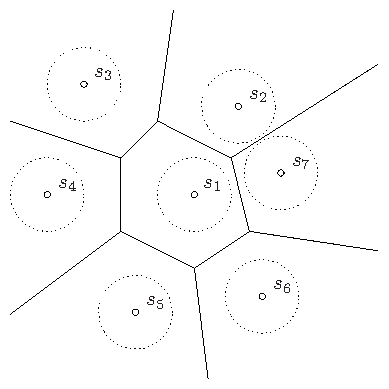
\includegraphics[width=.70\textwidth]{figures/ch07-figure-5.pdf}
\caption*{图7.5\quad 七个信号 $s_1,\ldots,s_7\in\R^2$ 构成的星座，以小圆圈表示。线段给出相应Voronoi区域的边界。当接收信号比起其他点更接近 $s_k$ 时，即位于 $s_k$ 的Voronoi区域内部时，最小距离检测器选择符号 $s_k$。每个点周围的大圆半径为一，用于展示尺度。}
\end{figure}

\subsubsection*{Chebyshev界}
半正定规划界（7.19）给出正确检测概率的下界。图7.6画出对 $s_1,s_2,s_3$ 三个符号，这些下界随噪声标准差 $\sigma$ 的变化。它们适用于任意零均值、协方差为 $\sigma^2I$ 的噪声分布。这些界是紧的，含义是：存在一个零均值、协方差 $\Sigma=\sigma^2I$ 的噪声分布，使错误概率等于该下界。图7.7给出第一个Voronoi集合、$\sigma=1$ 时的情形。

\subsubsection*{Chernoff界}
用同一例子说明Chernoff界。此时假设噪声高斯，即 $v\sim N(0,\sigma^2I)$。若发送符号 $s_k$，正确检测概率为 $\Prob(s_k+v\in V_k)$。为求该概率的下界，用二次规划（7.21）计算ML检测器选择符号 $i$ 的概率上界，$i=1,\ldots,m$、$i\ne k$。这些上界分别与 $s_k$ 到Voronoi集 $V_i$ 的距离有关。把将 $s_k$ 误作 $s_i$ 的各概率上界相加，得到错误概率上界，进而得到正确检测 $s_k$ 的概率下界。图7.8给出 $s_1$ 的下界，以及由Monte Carlo分析获得的正确检测概率估计。

% Source PDF page 397 (printed p. 383)
\begin{figure}[htbp]\centering
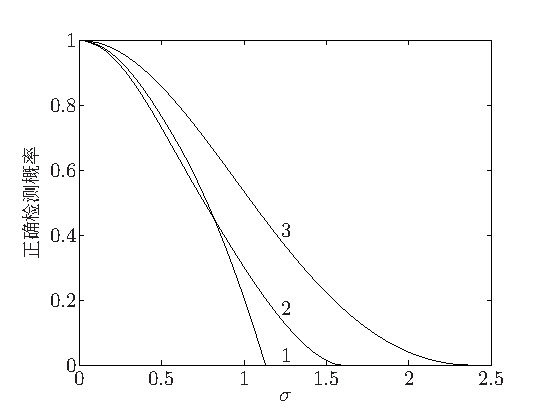
\includegraphics[width=.70\textwidth]{figures/ch07-figure-6.pdf}
\caption*{图7.6\quad 符号 $s_1,s_2,s_3$ 正确检测概率的Chebyshev下界。对所有零均值、协方差为 $\sigma^2I$ 的噪声分布，这些界都成立。}
\end{figure}
\begin{figure}[htbp]\centering
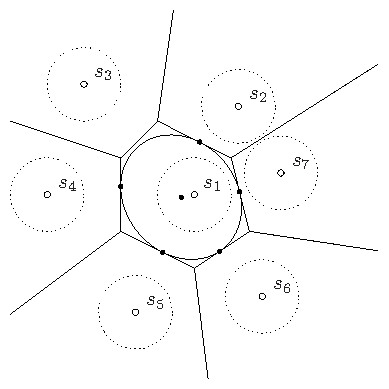
\includegraphics[width=.70\textwidth]{figures/ch07-figure-7.pdf}
\caption*{图7.7\quad $\sigma=1$ 时，正确检测符号1的概率的Chebyshev下界为0.2048，图示离散分布取到这一界。实心圆为接收信号 $s_1+v$ 的可能值。椭圆中心处的点概率为0.2048，边界上五个点的总概率为0.7952。椭圆由 $x^{\T}Px+2q^{\T}x+r=1$ 定义，其中 $P,q,r$ 为半正定规划（7.19）的最优解。}
\end{figure}

% Source PDF page 398 (printed p. 384)
\begin{figure}[htbp]\centering
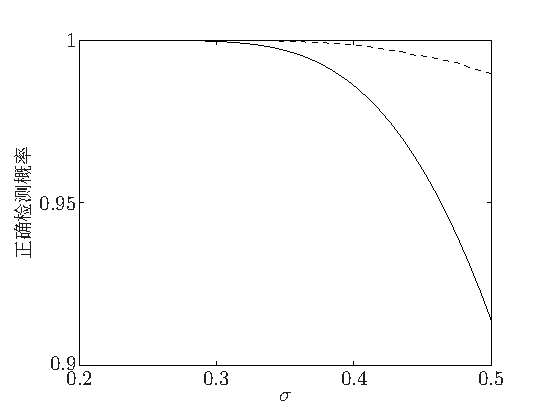
\includegraphics[width=.70\textwidth]{figures/ch07-figure-8.pdf}
\caption*{图7.8\quad 正确检测符号 $s_1$ 的概率随 $\sigma$ 变化的Chernoff下界（实线）和Monte Carlo估计（虚线）。本例噪声为零均值、协方差 $\sigma^2I$ 的高斯噪声。}
\end{figure}

\section{实验设计}
考虑根据测量或实验
\[
 y_i=a_i^{\T}x+w_i,\qquad i=1,\ldots,m
\]
估计向量 $x\in\R^n$，其中 $w_i$ 是测量噪声。假设 $w_i$ 是相互独立、零均值、单位方差的高斯随机变量，测量向量 $a_1,\ldots,a_m$ 张成 $\R^n$。$x$ 的最大似然估计与最小方差估计相同，均为最小二乘解
\[
 \widehat x=\left(\sum_{i=1}^ma_ia_i^{\T}\right)^{-1}
 \sum_{i=1}^my_ia_i.
\]
相应估计误差 $e=\widehat x-x$ 的均值为零，协方差矩阵为
\[
 E=\E ee^{\T}=\left(\sum_{i=1}^ma_ia_i^{\T}\right)^{-1}.
\]
矩阵 $E$ 刻画估计精度，或实验所提供的信息量。例如，$x$ 的 $\alpha$ 置信水平椭球为
\[
 \mathcal E=\{z\mid(z-\widehat x)^{\T}E^{-1}(z-\widehat x)\le\beta\},
\]
其中常数 $\beta$ 依赖于 $n,\alpha$。

假设表征测量的向量 $a_1,\ldots,a_m$，可以从 $p$ 个可能测试向量 $v_1,\ldots,v_p\in\R^n$ 中选择，即每个 $a_i$ 都是某个 $v_j$。

% Source PDF page 399 (printed p. 385)
\emph{实验设计}的目标是从可能向量中选择 $a_i$，使误差协方差 $E$ 在某种意义下尽量小。换言之，$m$ 次实验或测量中的每一次，都从固定的 $p$ 种可能实验中选择；任务是找到一组联合起来信息量最大的测量。

用 $m_j$ 表示选择 $a_i=v_j$ 的实验次数，有
\[
 m_1+\cdots+m_p=m.
\]
误差协方差矩阵可表示为
\[
 E=\left(\sum_{i=1}^ma_ia_i^{\T}\right)^{-1}
 =\left(\sum_{j=1}^pm_jv_jv_j^{\T}\right)^{-1}.
\]
这表明误差协方差只依赖于每类实验所选择的次数，即 $m_1,\ldots,m_p$。

基本实验设计问题如下：给定可能实验的选项 $v_1,\ldots,v_p$ 和要进行的总实验次数 $m$，选择每类实验的次数 $m_1,\ldots,m_p$，使误差协方差 $E$ 在某种意义下尽量小。变量 $m_1,\ldots,m_p$ 当然必须为整数，并且总和等于给定实验总次数 $m$。得到优化问题
\begin{equation}
\begin{array}{ll}
\text{最小化（关于 }\mathbf S_+^n\text{）}
 &\displaystyle E=\left(\sum_{j=1}^pm_jv_jv_j^{\T}\right)^{-1}\\[4pt]
\text{满足}&m_i\ge0,\quad m_1+\cdots+m_p=m,\\
&m_i\in\Z,
\end{array}\tag{7.23}
\end{equation}
变量为整数 $m_1,\ldots,m_p$。

基本实验设计问题（7.23）是半正定锥上的向量优化问题。如果一种设计得到 $E$，另一种得到 $\widetilde E$，且 $E\preceq\widetilde E$，那么第一种设计肯定不比第二种差。例如，把置信椭球平移到原点以便比较时，第一种设计的置信椭球包含在第二种之中。还可以说，对任意向量 $q$，第一种设计对 $q^{\T}x$ 的估计都更好，即方差更低，因为两种设计下 $q^{\T}x$ 估计的方差分别为 $q^{\T}Eq$ 和 $q^{\T}\widetilde Eq$。下面将介绍几种常见标量化形式。

\subsection{松弛的实验设计问题}
当总实验次数 $m$ 与 $p$ 相当时，（7.23）可能是困难的组合问题，因为此时各 $m_i$ 都是小整数。但当 $m$ 远大于 $p$ 时，通过忽略或松弛 $m_i$ 的整数约束，可找到（7.23）的良好近似解。令 $\lambda_i=m_i/m$，表示 $a_j=v_i$ 的实验占总实验次数的比例，或第 $i$ 类实验的相对频率。

% Source PDF page 400 (printed p. 386)
用 $\lambda_i$ 可将误差协方差表示为
\begin{equation}
 E=\frac1m\left(\sum_{i=1}^p\lambda_iv_iv_i^{\T}\right)^{-1}.\tag{7.24}
\end{equation}
向量 $\lambda\in\R^p$ 满足 $\lambda\succeq0$、$\one^{\T}\lambda=1$，且每个 $\lambda_i$ 都是 $1/m$ 的整数倍。忽略最后这一约束，就得到问题
\begin{equation}
\begin{array}{ll}
\text{最小化（关于 }\mathbf S_+^n\text{）}
 &\displaystyle E=\frac1m\left(\sum_{i=1}^p\lambda_iv_iv_i^{\T}\right)^{-1}\\[4pt]
\text{满足}&\lambda\succeq0,\quad\one^{\T}\lambda=1,
\end{array}\tag{7.25}
\end{equation}
变量为 $\lambda\in\R^p$。为区别于原来的组合实验设计问题（7.23），称其为\emph{松弛的实验设计问题}。由于目标 $E$ 是 $\lambda$ 的 $\mathbf S_+^n$ 凸函数，（7.25）是凸优化问题。

组合实验设计问题（7.23）与松弛问题（7.25）之间有以下联系。显然，组合问题多了一个约束，因此松弛问题的最优值为组合问题的最优值提供下界。由松弛解可按以下方式构造组合问题的一个次优解。先简单舍入：
\[
 m_i=\operatorname{round}(m\lambda_i),\qquad i=1,\ldots,p.
\]
对应这一选择的向量 $\widetilde\lambda$ 为
\[
 \widetilde\lambda_i=(1/m)\operatorname{round}(m\lambda_i),\qquad i=1,\ldots,p.
\]
$\widetilde\lambda$ 每个分量都是 $1/m$ 的整数倍。显然，$\abs{\lambda_i-\widetilde\lambda_i}\le1/(2m)$，所以当 $m$ 大时，$\lambda\approx\widetilde\lambda$。这意味着约束 $\one^{\T}\widetilde\lambda=1$ 在 $m$ 很大时近似满足，也意味着两者相应的误差协方差矩阵接近。

松弛问题（7.25）还有另一种解释：把 $\lambda\in\R^p$ 看作实验 $v_1,\ldots,v_p$ 上的概率分布。选择 $\lambda$ 对应一个随机实验：每次实验 $a_i$ 以概率 $\lambda_j$ 取 $v_j$。

本节余下只讨论松弛的实验设计问题，因此省略“松弛”这一修饰。

\subsection{标量化}
对于半正定锥上的向量优化问题（7.25），人们提出了几种标量化方式。

% Source PDF page 401 (printed p. 387)
\subsubsection*{D最优设计}
使用最广泛的标量化称为\emph{D最优设计}，它最小化误差协方差矩阵 $E$ 的行列式，对应于在置信水平固定时，最小化所得置信椭球的体积。忽略 $E$ 中常数因子 $1/m$，再对目标取对数，问题可写成
\begin{equation}
\begin{array}{ll}
\text{最小化}&\displaystyle\log\det\left(\sum_{i=1}^p\lambda_iv_iv_i^{\T}\right)^{-1}\\[4pt]
\text{满足}&\lambda\succeq0,\quad\one^{\T}\lambda=1,
\end{array}\tag{7.26}
\end{equation}
它是凸优化问题。

\subsubsection*{E最优设计}
\emph{E最优设计}最小化误差协方差矩阵的范数，即 $E$ 的最大特征值。置信椭球 $\mathcal E$ 的直径，也就是最长半轴的两倍，正比于 $\norm E_2^{1/2}$，所以最小化 $\norm E_2$，在几何上相当于最小化置信椭球直径。E最优设计也可解释为，在所有 $\norm q_2=1$ 的 $q$ 中，使 $q^{\T}e$ 的最大方差最小。E最优实验设计问题为
\[
\begin{array}{ll}
\text{最小化}&\displaystyle\left\|\left(\sum_{i=1}^p\lambda_iv_iv_i^{\T}\right)^{-1}\right\|_2\\[4pt]
\text{满足}&\lambda\succeq0,\quad\one^{\T}\lambda=1.
\end{array}
\]
目标关于 $\lambda$ 凸，因此该问题凸。

E最优设计也可写成半正定规划
\begin{equation}
\begin{array}{ll}
\text{最大化}&t\\
\text{满足}&\displaystyle\sum_{i=1}^p\lambda_iv_iv_i^{\T}\succeq tI,\\
&\lambda\succeq0,\quad\one^{\T}\lambda=1,
\end{array}\tag{7.27}
\end{equation}
变量为 $\lambda\in\R^p$、$t\in\R$。

\subsubsection*{A最优设计}
\emph{A最优实验设计}最小化协方差矩阵的迹 $\tr E$。该目标就是误差范数平方的均值：
\[
 \E\norm e_2^2=\E\tr(ee^{\T})=\tr E.
\]
A最优实验设计问题为
\begin{equation}
\begin{array}{ll}
\text{最小化}&\displaystyle\tr\left(\sum_{i=1}^p\lambda_iv_iv_i^{\T}\right)^{-1}\\[4pt]
\text{满足}&\lambda\succeq0,\quad\one^{\T}\lambda=1.
\end{array}\tag{7.28}
\end{equation}
这同样是凸问题，也能像E最优设计那样写成半正定规划：
\[
\begin{array}{ll}
\text{最小化}&\one^{\T}u\\[3pt]
\text{满足}&\displaystyle\begin{bmatrix}
 \sum_{i=1}^p\lambda_iv_iv_i^{\T}&e_k\\e_k^{\T}&u_k
 \end{bmatrix}\succeq0,\quad k=1,\ldots,n,\\[4pt]
&\lambda\succeq0,\quad\one^{\T}\lambda=1,
\end{array}
\]

% Source PDF page 402 (printed p. 388)
变量为 $u\in\R^n$ 和 $\lambda\in\R^p$，$e_k$ 为第 $k$ 个单位向量。

\subsubsection*{最优实验设计与对偶性}
三种标量化问题的拉格朗日对偶具有有趣的几何意义。

D最优实验设计（7.26）的对偶可写为
\[
\begin{array}{ll}
\text{最大化}&\log\det W+n\log n\\
\text{满足}&v_i^{\T}Wv_i\le1,\quad i=1,\ldots,p,
\end{array}
\]
变量为 $W\in\mathbf S^n$，定义域为 $\mathbf S_{++}^n$，见习题5.10。这个对偶问题有简单解释：最优解 $W^\star$ 确定包含 $v_1,\ldots,v_p$、以原点为中心的最小体积椭球 $\{x\mid x^{\T}W^\star x\le1\}$，另见第222页问题（5.14）的讨论。由互补松弛，
\begin{equation}
 \lambda_i^\star(1-v_i^{\T}W^\star v_i)=0,\qquad i=1,\ldots,p,\tag{7.29}
\end{equation}
即最优设计仅使用位于该最小体积椭球表面上的实验 $v_i$。

E最优与A最优设计的对偶也有类似解释。问题（7.27）、（7.28）的对偶分别可写成
\begin{equation}
\begin{array}{ll}
\text{最大化}&\tr W\\
\text{满足}&v_i^{\T}Wv_i\le1,\quad i=1,\ldots,p,\\
&W\succeq0,
\end{array}\tag{7.30}
\end{equation}
以及
\begin{equation}
\begin{array}{ll}
\text{最大化}&(\tr W^{1/2})^2\\
\text{满足}&v_i^{\T}Wv_i\le1,\quad i=1,\ldots,p.
\end{array}\tag{7.31}
\end{equation}
两者的变量均为 $W\in\mathbf S^n$，第二个问题还有隐式约束 $W\in\mathbf S_+^n$，见习题5.40与5.10。

与D最优设计一样，最优解 $W^\star$ 确定一个包含 $v_1,\ldots,v_p$ 的极小椭球 $\{x\mid x^{\T}W^\star x\le1\}$。此外，$W^\star$ 与 $\lambda^\star$ 满足互补松弛（7.29），即最优设计只使用位于 $W^\star$ 所定义椭球表面的实验 $v_i$。

\subsubsection*{实验设计例子}
考虑 $x\in\R^2$、$p=20$ 的问题。图7.9用圆圈表示20个候选测量向量 $a_i$，原点以叉号表示。D最优实验只有两个非零 $\lambda_i$，以实心圆标在图7.9中；E最优实验也只有两个非零 $\lambda_i$，见图7.10；A最优实验有三个非零 $\lambda_i$，见图7.11。图中还画出三个与对偶最优解 $W^\star$ 关联的椭球 $\{x\mid x^{\T}W^\star x\le1\}$。图7.12给出所得90\%置信椭球，以及对所有实验赋予等权 $\lambda_i=1/p$ 的“均匀”设计的置信椭球。

% Source PDF page 403 (printed p. 389)
\begin{figure}[htbp]\centering
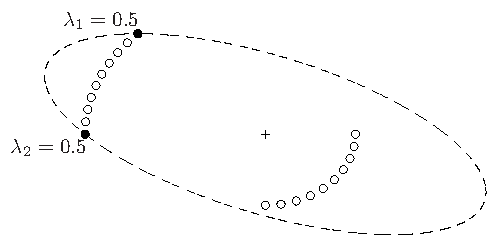
\includegraphics[width=.68\textwidth]{figures/ch07-figure-9.pdf}
\caption*{图7.9\quad 实验设计例子。20个候选测量向量以圆圈表示。D最优设计使用两个实心圆所示的测量向量，并各赋予相同权重 $\lambda_i=0.5$。椭球是包含各点 $v_i$、以原点为中心的最小体积椭球。}
\end{figure}
\begin{figure}[htbp]\centering
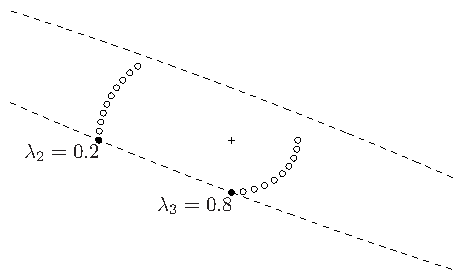
\includegraphics[width=.68\textwidth]{figures/ch07-figure-10.pdf}
\caption*{图7.10\quad E最优设计使用两个测量向量。虚线为椭球 $\{x\mid x^{\T}W^\star x\le1\}$ 的部分边界，其中 $W^\star$ 是对偶问题（7.30）的解。}
\end{figure}
\begin{figure}[htbp]\centering
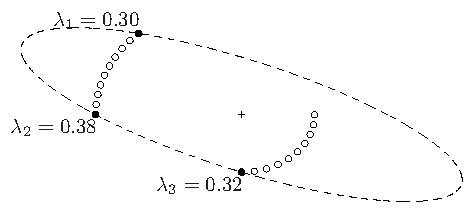
\includegraphics[width=.68\textwidth]{figures/ch07-figure-11.pdf}
\caption*{图7.11\quad A最优设计使用三个测量向量。虚线为对偶问题（7.31）的解所对应的椭球 $\{x\mid x^{\T}W^\star x\le1\}$。}
\end{figure}

% Source PDF page 404 (printed p. 390)
\begin{figure}[htbp]\centering
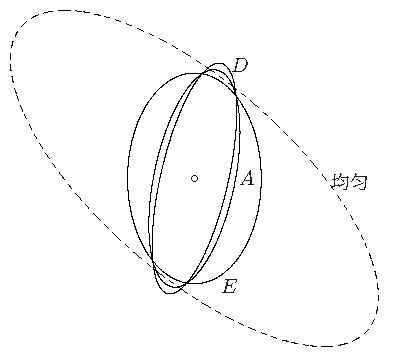
\includegraphics[width=.70\textwidth]{figures/ch07-figure-12.pdf}
\caption*{图7.12\quad D最优、A最优、E最优和均匀设计的90\%置信椭球形状。}
\end{figure}

\subsection{扩展}
\subsubsection*{资源限制}
假设每类实验有相应代价 $c_i$，它可以表示用 $v_i$ 进行一次实验的经济成本或所需时间。总成本，或实验顺序执行时的总时间，为
\[
 m_1c_1+\cdots+m_pc_p=mc^{\T}\lambda.
\]
可在基本实验设计问题中加入线性不等式 $mc^{\T}\lambda\le B$，其中 $B$ 为预算，以限制总成本。也可以加入多个线性不等式，表示多项资源的限制。

\subsubsection*{每次实验进行多个测量}
还可以推广到每次实验产生多个测量的情形。换言之，选择某个可能实验并执行后，会获得若干测量。可沿用前面的记号，将 $v_i$ 取为 $\R^{n\times k_i}$ 中的矩阵：
\[
 v_i=\begin{bmatrix}u_{i1}&\cdots&u_{ik_i}\end{bmatrix},
\]
其中 $k_i$ 是执行实验 $v_i$ 后得到的标量测量个数。在这种更复杂的设定下，误差协方差矩阵的形式完全不变。

结合表示成本或时间限制的附加线性不等式，可以描述同时进行一组测量带来的成本优惠或时间节省。例如，假设同时进行标量测量 $v_1,v_2$ 的成本，低于分别进行两次测量的成本之和。

% Source PDF page 405 (printed p. 391)
令 $v_3$ 为矩阵
\[
 v_3=\begin{bmatrix}v_1&v_2\end{bmatrix},
\]
并用 $c_1,c_2,c_3$ 分别表示单独进行第一个测量、单独进行第二个测量，以及同时进行两者的成本。

求解实验设计问题后，$\lambda_1$ 给出应单独进行第一个实验的次数比例，$\lambda_2$ 给出单独进行第二个实验的比例，$\lambda_3$ 给出同时进行两个实验的比例。通常会预期这几类中有所取舍，不会同时出现 $\lambda_1>0$、$\lambda_2>0$、$\lambda_3>0$。

% Source PDF page 406 (printed p. 392)
\section*{文献说明}
\addcontentsline{toc}{section}{文献说明}
ML和MAP估计、假设检验与检测，可参阅统计学、模式识别、统计信号处理或通信方面的书籍，例如 Bickel 和 Doksum [BD77]，Duda、Hart 和 Stork [DHS99]，Scharf [Sch91]，或 Proakis [Pro01]。

Logistic回归见 Hastie、Tibshirani 和 Friedman [HTF01，第4.4节]。第355页的协方差估计问题见 Anderson [And70]。

20世纪60年代，Isii [Isi64]、Marshall 和 Olkin [MO60]、Karlin 和 Studden [KS66，第12章] 等对Chebyshev不等式的推广进行了广泛研究。较近，Bertsimas 和 Sethuraman [BS00]、Lasserre [Las02] 建立了其与半正定规划的联系。

第7.5节中的A、D、E最优性是最优实验设计文献中的标准术语，例如 Pukelsheim [Puk93]。D最优设计对偶问题的几何解释见 Titterington [Tit75]。

% Source PDF page 407 (printed p. 393)
\section*{习题}
\addcontentsline{toc}{section}{习题}
\subsection*{估计}
\paragraph{7.1}
\textbf{指数分布噪声下的线性测量。}说明噪声服从指数分布时，如何求解ML估计问题（7.2），其密度为
\[
 p(z)=\begin{cases}(1/a)e^{-z/a}&z\ge0,\\0&z<0,\end{cases}
\]
其中 $a>0$。

\paragraph{7.2}
\textbf{ML估计与 $\ell_\infty$ 范数逼近。}考虑第352页的线性测量模型 $y=Ax+v$，噪声均匀分布，密度为
\[
 p(z)=\begin{cases}1/(2\alpha)&\abs z\le\alpha,\\0&\abs z>\alpha.\end{cases}
\]
如第352页例7.1所述，任意满足 $\norm{Ax-y}_\infty\le\alpha$ 的 $x$ 都是ML估计。

现设参数 $\alpha$ 未知，需要将它与 $x$ 一起估计。证明：求解 $\ell_\infty$ 范数逼近问题
\[
 \text{最小化}\quad\norm{Ax-y}_\infty
\]
即可找到 $x,\alpha$ 的ML估计，其中 $a_i^{\T}$ 为 $A$ 的各行。

\paragraph{7.3}
\textbf{Probit模型。}设随机变量 $y\in\{0,1\}$ 由下式给出：
\[
 y=\begin{cases}1&a^{\T}u+b+v\le0,\\0&a^{\T}u+b+v>0,\end{cases}
\]
其中 $u\in\R^n$ 是解释变量向量，与第354页Logistic模型中的意义相同，$v$ 为零均值、单位方差的高斯变量。

给定数据对 $(u_i,y_i)$，$i=1,\ldots,N$，将估计 $a,b$ 的ML问题写成凸优化问题。

\paragraph{7.4}
\textbf{多元正态分布的协方差与均值估计。}考虑根据 $N$ 个独立样本 $y_1,y_2,\ldots,y_N\in\R^n$，估计高斯概率密度
\[
 p_{R,a}(y)=(2\pi)^{-n/2}\det(R)^{-1/2}
 \exp\bigl(-(y-a)^{\T}R^{-1}(y-a)/2\bigr)
\]
的协方差矩阵 $R$ 与均值 $a$。
\begin{enumerate}[label=(\alph*)]
\item 先考虑对 $R,a$ 没有附加约束的估计问题。令 $\mu,Y$ 为样本均值与协方差，定义为
\[
 \mu=\frac1N\sum_{k=1}^Ny_k,\qquad
 Y=\frac1N\sum_{k=1}^N(y_k-\mu)(y_k-\mu)^{\T}.
\]
证明对数似然函数
\[
 l(R,a)=-(Nn/2)\log(2\pi)-(N/2)\log\det R
 -(1/2)\sum_{k=1}^N(y_k-a)^{\T}R^{-1}(y_k-a)
\]

% Source PDF page 408 (printed p. 394)
可表示为
\[
 l(R,a)=\frac N2\bigl(-n\log(2\pi)-\log\det R
 -\tr(R^{-1}Y)-(a-\mu)^{\T}R^{-1}(a-\mu)\bigr).
\]
利用该表达式证明：若 $Y\succ0$，$R,a$ 的ML估计唯一，且为
\[
 a_{\mathrm{ml}}=\mu,\qquad R_{\mathrm{ml}}=Y.
\]
\item 对数似然函数包含凸项 $-\log\det R$，因此其凹性并不显然。证明：在区域
\[
 R\preceq2Y
\]
内，$l$ 关于 $R,a$ 联合凹。这意味着，只要约束包含 $R\preceq2Y$，即 $R$ 的估计不超过无约束ML估计的两倍，就可以在凸约束下，用凸优化同时计算 $R,a$ 的ML估计。
\end{enumerate}

\paragraph{7.5}
\textbf{Markov链估计。}考虑一个具有 $n$ 个状态的Markov链，转移概率矩阵 $P\in\R^{n\times n}$ 定义为
\[
 P_{ij}=\Prob(y(t+1)=i\mid y(t)=j).
\]
转移概率必须满足 $P_{ij}\ge0$、$\sum_{i=1}^nP_{ij}=1$，$j=1,\ldots,n$。考虑由观测样本序列 $y(1)=k_1$、$y(2)=k_2$、$\ldots$、$y(N)=k_n$ 估计转移概率。
\begin{enumerate}[label=(\alph*)]
\item 证明：若 $P_{ij}$ 无其他先验约束，其ML估计为经验转移频率：$\widehat P_{ij}$ 是观测样本中状态从 $j$ 转移到 $i$ 的次数，与状态为 $j$ 的次数之比。
\item 假设Markov链的一个平衡分布 $p$ 已知，即向量 $q\in\R_+^n$ 满足 $\one^{\T}q=1$、$Pq=q$。证明根据观测序列及已知 $q$ 求 $P$ 的ML估计，可以表示为凸优化问题。
\end{enumerate}

\paragraph{7.6}
\textbf{均值与方差估计。}考虑密度为 $p$ 的随机变量 $x\in\R$，它已标准化，即零均值、单位方差。对 $x$ 作仿射变换得到 $y=(x+b)/a$，其中 $a>0$。$y$ 的均值为 $b/a$，方差为 $1/a^2$。当 $a,b$ 分别在 $\R_+$、$\R$ 上变化时，通过缩放与平移 $p$，产生由均值和方差唯一参数化的一族密度。

证明：若 $p$ 对数凹，给定 $y$ 的样本 $y_1,\ldots,y_n$，求 $a,b$ 的ML估计是凸问题。

作为例子，假设 $p$ 是标准化的Laplace密度 $p(x)=e^{-2\abs x}$，求出 $a,b$ 的ML估计的解析解。

\paragraph{7.7}
\textbf{Poisson分布的ML估计。}设随机变量 $x_i$，$i=1,\ldots,n$，相互独立，服从Poisson分布
\[
 \Prob(x_i=k)=\frac{e^{-\mu_i}\mu_i^k}{k!},
\]
均值 $\mu_i$ 未知。$x_i$ 表示某段时间内 $n$ 类可能独立事件中，第 $i$ 类发生的次数。例如，在发射断层成像中，它们可以表示 $n$ 个源发射的光子数。

考虑一个用于确定均值 $\mu_i$ 的实验，其中有 $m$ 个检测器。若发生事件 $i$，则它以概率 $p_{ji}$ 被检测器 $j$ 检出。

% Source PDF page 409 (printed p. 395)
假设概率 $p_{ji}$ 已知，且 $p_{ji}\ge0$、$\sum_{j=1}^mp_{ji}\le1$。检测器 $j$ 记录的事件总数记为 $y_j$，
\[
 y_j=\sum_{i=1}^ny_{ji},\qquad j=1,\ldots,m.
\]
根据观测值 $y_j$，$j=1,\ldots,m$，将估计均值 $\mu_i$ 的ML问题写成凸优化问题。

\emph{提示：}变量 $y_{ji}$ 服从均值为 $p_{ji}\mu_i$ 的Poisson分布，即
\[
 \Prob(y_{ji}=k)=\frac{e^{-p_{ji}\mu_i}(p_{ji}\mu_i)^k}{k!}.
\]
均值分别为 $\lambda_1,\ldots,\lambda_n$ 的 $n$ 个独立Poisson变量之和，仍服从Poisson分布，均值为 $\lambda_1+\cdots+\lambda_n$。

\paragraph{7.8}
\textbf{利用符号测量的估计。}考虑测量模型
\[
 y_i=\operatorname{sign}(a_i^{\T}x+b_i+v_i),\qquad i=1,\ldots,m,
\]
其中 $x\in\R^n$ 为待估向量，$y_i\in\{-1,1\}$ 为测量值。向量 $a_i\in\R^n$、标量 $b_i\in\R$ 已知，$v_i$ 是独立同分布、具有对数凹概率密度的噪声。可假设 $a_i^{\T}x+b_i+v_i=0$ 不会发生。证明 $x$ 的最大似然估计是凸优化问题。

\paragraph{7.9}
\textbf{传感器非线性未知时的估计。}考虑测量模型
\[
 y_i=f(a_i^{\T}x+b_i+v_i),\qquad i=1,\ldots,m,
\]
其中 $x\in\R^n$ 为待估向量，$y_i\in\R$ 为测量值，$a_i\in\R^n$、$b_i\in\R$ 已知，$v_i$ 为独立同分布、密度对数凹的噪声。表示测量非线性的函数 $f:\R\to\R$ 未知，但已知它对所有 $t$ 满足 $f'(t)\in[l,u]$，其中 $0<l<u$ 已知。

说明如何用凸优化找到 $x$ 以及函数 $f$ 的最大似然估计。这是无限维ML估计问题，但可以采用非正式的处理和解释。

\paragraph{7.10}
\textbf{$\R^k$ 上的非参数分布。}考虑随机变量 $x\in\R^k$，取值于有限集 $\{\alpha_1,\ldots,\alpha_n\}$，分布为
\[
 p_i=\Prob(x=\alpha_i),\qquad i=1,\ldots,n.
\]
证明 $X$ 的协方差下界
\[
 S\preceq\E(X-\E X)(X-\E X)^{\T}
\]
是关于 $p$ 的凸约束。

\subsection*{最优检测器设计}
\paragraph{7.11}
\textbf{随机化检测器。}证明每个随机化检测器都能表示为一组确定性检测器的凸组合：若
\[
 T=\begin{bmatrix}t_1&t_2&\cdots&t_n\end{bmatrix}\in\R^{m\times n}
\]
满足 $t_k\succeq0$、$\one^{\T}t_k=1$，则可写为
\[
 T=\theta_1T_1+\cdots+\theta_NT_N,
\]

% Source PDF page 410 (printed p. 396)
其中 $T_i$ 是每列恰有一个元素为一的0--1矩阵，$\theta_i\ge0$、$\sum_{i=1}^N\theta_i=1$。最多可能需要多少个确定性检测器，即 $N$ 最大需要多大？

可作如下解释：随机化检测器能够由 $N$ 个确定性检测器组成的检测器组实现。观测到 $X=k$ 时，估计器从 $\{1,\ldots,N\}$ 中以概率 $\Prob(j=i)=\theta_i$ 选取随机索引，再使用确定性检测器 $T_j$。

\paragraph{7.12}
\textbf{最优行动。}检测器设计中，给定各列为概率分布的矩阵 $P\in\R^{n\times m}$，然后设计各列也为概率分布的矩阵 $T\in\R^{m\times n}$，使 $D=TP$ 的对角元大、非对角元小。本题研究对应的对偶问题：给定 $P$，寻找各列为概率分布的矩阵 $S\in\R^{m\times n}$，使 $\widetilde D=PS\in\R^{n\times n}$ 对角元大、非对角元小。具体取目标为最大化 $\widetilde D$ 的最小对角元。

可作如下解释：有 $n$ 种结果，其发生概率取决于采取 $m$ 种输入或行动中的哪一种；$P_{ij}$ 是采取行动 $j$ 时出现结果 $i$ 的概率。目标是寻找一种随机化策略，使任何指定结果尽可能发生。策略由矩阵 $S$ 给出：希望结果 $i$ 发生时，以概率 $S_{ji}$ 采取行动 $j$。矩阵 $\widetilde D$ 给出行动错误概率矩阵：$\widetilde D_{ij}$ 是希望结果 $j$ 发生时，实际出现结果 $i$ 的概率。特别地，$\widetilde D_{ii}$ 是希望结果 $i$ 发生时，结果 $i$ 实际发生的概率。

证明这个问题具有简单解析解。证明与相应检测器问题不同，这里总有确定性的最优解。

\emph{提示：}证明问题关于 $S$ 的各列可分。

\subsection*{Chebyshev界与Chernoff界}
\paragraph{7.13}
\textbf{有限集上的Chebyshev型不等式。}设随机变量 $X$ 取值于集合 $\{\alpha_1,\alpha_2,\ldots,\alpha_m\}$，$S$ 是 $\{\alpha_1,\ldots,\alpha_m\}$ 的子集。$X$ 的分布未知，但已知 $n$ 个函数 $f_i$ 的期望：
\begin{equation}
 \E f_i(X)=b_i,\qquad i=1,\ldots,n.\tag{7.32}
\end{equation}
证明线性规划
\[
\begin{array}{ll}
\text{最小化}&\displaystyle x_0+\sum_{i=1}^nb_ix_i\\
\text{满足}&\displaystyle x_0+\sum_{i=1}^nf_i(\alpha)x_i\ge1,\quad\alpha\in S,\\
&\displaystyle x_0+\sum_{i=1}^nf_i(\alpha)x_i\ge0,\quad\alpha\notin S,
\end{array}
\]
的最优值为 $\Prob(X\in S)$ 的上界，对所有满足（7.32）的分布都成立，变量为 $x_0,\ldots,x_n$。证明总存在某个分布取到该上界。


% Source PDF page 411 (printed p. 397)
\chapter{几何问题}
\section{在集合上的投影}
点 $x_0\in\R^n$ 到闭集 $C\subseteq\R^n$ 在范数 $\norm{\cdot}$ 下的距离定义为
\[\dist(x_0,C)=\inf\{\norm{x_0-x}\mid x\in C\}.\]
这里的下确界总能取到。把任意离 $x_0$ 最近的点 $z\in C$，即满足 $\norm{z-x_0}=\dist(x_0,C)$ 的点，称为 $x_0$ 在 $C$ 上的一个投影。一般而言，$x_0$ 在 $C$ 上可以有多个投影，即 $C$ 中可以有多个点离 $x_0$ 最近。

在一些特殊情况下，可以证明点在集合上的投影唯一。例如，若 $C$ 闭且凸，范数严格凸（例如欧氏范数），则对任意 $x_0$，总恰好存在一个离 $x_0$ 最近的 $z\in C$。一个有趣的逆命题是：若对每个 $x_0$，它在 $C$ 上的欧氏投影都唯一，则 $C$ 闭且凸，见习题8.2。

用 $P_C:\R^n\to\R^n$ 表示任意满足 $P_C(x_0)$ 是 $x_0$ 在 $C$ 上投影的函数，即对所有 $x_0$ 有
\[P_C(x_0)\in C,\qquad\norm{x_0-P_C(x_0)}=\dist(x_0,C).\]
换句话说，
\[P_C(x_0)=\argmin\{\norm{x-x_0}\mid x\in C\}.\]
称 $P_C$ 为在 $C$ 上的投影。
\begin{origexample}{8.1}
\textbf{在 $\R^2$ 的单位正方形上的投影。}考虑 $\R^2$ 中单位正方形的边界，即 $C=\{x\in\R^2\mid\norm x_\infty=1\}$，取 $x_0=0$。

在 $\ell_1$ 范数下，四个点 $(1,0),(0,-1),(-1,0),(0,1)$ 离 $x_0=0$ 最近，距离为一，因此 $\ell_1$ 范数下 $\dist(x_0,C)=1$。$\ell_2$ 范数下结论相同。

在 $\ell_\infty$ 范数下，$C$ 中所有点与 $x_0$ 的距离都为一，$\dist(x_0,C)=1$。
\end{origexample}
% Source PDF page 412 (printed p. 398)
\begin{origexample}{8.2}
\textbf{在秩不超过 $k$ 的矩阵集合上的投影。}考虑秩小于等于 $k$ 的 $m\times n$ 矩阵集合
\[C=\{X\in\R^{m\times n}\mid\rank X\leq k\},\]
其中 $k\leq\min\{m,n\}$，设 $X_0\in\R^{m\times n}$。可以用奇异值分解求出 $X_0$ 在 $C$ 上关于谱范数（最大奇异值范数）$\norm{\cdot}_2$ 的一个投影。设
\[X_0=\sum_{i=1}^r\sigma_i u_iv_i^\T\]
是 $X_0$ 的奇异值分解，其中 $r=\rank X_0$。则矩阵 $Y=\sum_{i=1}^{\min\{k,r\}}\sigma_i u_iv_i^\T$ 为 $X_0$ 在 $C$ 上的一个投影。
\end{origexample}
\subsection{将点投影到凸集上}
若 $C$ 凸，则可以通过求解凸优化问题，计算投影 $P_C(x_0)$ 与距离 $\dist(x_0,C)$。用一组线性等式与凸不等式表示 $C$：
\begin{equation}Ax=b,\qquad f_i(x)\leq0,\quad i=1,\ldots,m,\tag{8.1}\end{equation}
通过求解以下问题找到 $x_0$ 在 $C$ 上的投影：
\begin{equation}
\begin{array}{ll}
 \text{最小化}&\norm{x-x_0}\\
 \text{约束为}&f_i(x)\leq0,\quad i=1,\ldots,m,\\
 &Ax=b,
\end{array}\tag{8.2}
\end{equation}
变量为 $x$。问题可行当且仅当 $C$ 非空；可行时，其最优值为 $\dist(x_0,C)$，任意最优点都是 $x_0$ 在 $C$ 上的投影。
\subsubsection*{在多面体上的欧氏投影}
$x_0$ 在由线性不等式 $Ax\preceq b$ 描述的多面体上的投影，可以通过求解 QP
\[\begin{array}{ll}\text{最小化}&\norm{x-x_0}_2^2\\\text{约束为}&Ax\preceq b\end{array}\]
计算。有些特殊情况有简单的解析解。
\begin{itemize}
\item $x_0$ 在超平面 $C=\{x\mid a^\T x=b\}$ 上的欧氏投影为
\[P_C(x_0)=x_0+(b-a^\T x_0)a/\norm a_2^2.\]
\item $x_0$ 在半空间 $C=\{x\mid a^\T x\leq b\}$ 上的欧氏投影为
\[P_C(x_0)=\begin{cases}x_0+(b-a^\T x_0)a/\norm a_2^2,&a^\T x_0>b,\\x_0,&a^\T x_0\leq b.\end{cases}\]
% Source PDF page 413 (printed p. 399)
\item $x_0$ 在矩形 $C=\{x\mid l\preceq x\preceq u\}$（$l\prec u$）上的欧氏投影为
\[P_C(x_0)_k=\begin{cases}l_k,&x_{0k}\leq l_k,\\x_{0k},&l_k\leq x_{0k}\leq u_k,\\u_k,&x_{0k}\geq u_k.\end{cases}\]
\end{itemize}
\subsubsection*{在正常锥上的欧氏投影}
设 $x=P_K(x_0)$ 为点 $x_0$ 在正常锥 $K$ 上的欧氏投影。问题
\[\begin{array}{ll}\text{最小化}&\norm{x-x_0}_2^2\\\text{约束为}&x\succeq_K0\end{array}\]
的 KKT 条件为
\[x\succeq_K0,\qquad x-x_0=z,\qquad z\succeq_{K^*}0,\qquad z^\T x=0.\]
引入记号 $x_+=x$、$x_-=z$，可将这些条件写成
\[x_0=x_+-x_-,\quad x_+\succeq_K0,\quad x_-\succeq_{K^*}0,\quad x_+^\T x_-=0.\]
换句话说，通过把 $x_0$ 投影到锥 $K$ 上，就将它分解为两个正交元素之差：一个相对于 $K$ 非负，且是 $x_0$ 在 $K$ 上的投影；另一个相对于 $K^*$ 非负。

几个具体例子如下。
\begin{itemize}
\item 对 $K=\R_+^n$，$P_K(x_0)_k=\max\{x_{0k},0\}$。向量在非负正交象限上的欧氏投影，只需把每个负分量替换为零。
\item 对 $K=\mathbb S_+^n$ 以及欧氏范数，即 Frobenius 范数 $\norm{\cdot}_F$，有
\[P_K(X_0)=\sum_{i=1}^n\max\{0,\lambda_i\}v_iv_i^\T,\]
其中 $X_0=\sum_{i=1}^n\lambda_iv_iv_i^\T$ 为 $X_0$ 的特征值分解。将对称矩阵投影到半正定锥上，只需构造特征值展开并删去负特征值对应的项。此矩阵也是 $\ell_2$ 范数，即谱范数下在半正定锥上的投影。
\end{itemize}
\subsection{分离点与凸集}
设 $C$ 是由等式与不等式(8.1)描述的闭凸集。若 $x_0\in C$，则 $\dist(x_0,C)=0$，问题(8.2)的最优点为 $x_0$。若 $x_0\notin C$，则 $\dist(x_0,C)>0$，问题(8.2)的最优值为正。下面将看到，在这种情况下，任意对偶最优点都给出点 $x_0$ 与集合 $C$ 之间的一个分离超平面。

点在凸集上的投影与寻找分离二者的超平面（当点不在集合中时）之间存在联系，并不意外。事实上，2.5.1节中分离超平面定理的证明，就利用了寻找集合之间的欧氏距离。
% Source PDF page 414 (printed p. 400)
若 $P_C(x_0)$ 表示 $x_0$ 在 $C$ 上的欧氏投影，且 $x_0\notin C$，则超平面
\[(P_C(x_0)-x_0)^\T\bigl(x-\tfrac12(x_0+P_C(x_0))\bigr)=0\]
严格分离 $x_0$ 与 $C$，见图8.1。不过，在其他范数下，投影问题与分离超平面问题最清楚的联系是通过拉格朗日对偶建立的。
\begin{figure}[htbp]\centering
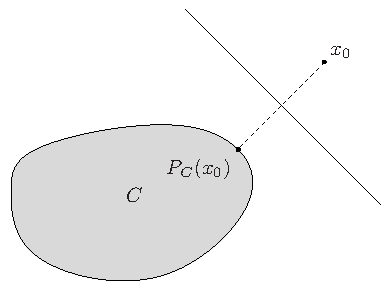
\includegraphics[width=.5\textwidth]{figures/ch08-414.pdf}
\caption*{图8.1 点 $x_0$ 及其在凸集 $C$ 上的欧氏投影 $P_C(x_0)$。位于两点中间、法向量为 $P_C(x_0)-x_0$ 的超平面，严格分离该点与集合。对一般范数，这一性质不成立，见习题8.4。}
\end{figure}
先将问题(8.2)写为
\[\begin{array}{ll}\text{最小化}&\norm y\\\text{约束为}&f_i(x)\leq0,\quad i=1,\ldots,m,\\&Ax=b,\\&x_0-x=y,\end{array}\]
变量为 $x,y$。拉格朗日函数为
\[L(x,y,\lambda,\mu,\nu)=\norm y+\sum_{i=1}^m\lambda_i f_i(x)+\nu^\T(Ax-b)+\mu^\T(x_0-x-y),\]
对偶函数为
\[g(\lambda,\mu,\nu)=\begin{cases}
 \displaystyle\inf_x\left(\sum_{i=1}^m\lambda_i f_i(x)+\nu^\T(Ax-b)+\mu^\T(x_0-x)\right),&\norm\mu_*\leq1,\\
 -\infty,&\text{其他情况}.
\end{cases}\]
于是得到对偶问题
\[\begin{array}{ll}
 \text{最大化}&\displaystyle\mu^\T x_0+\inf_x\left(\sum_{i=1}^m\lambda_if_i(x)+\nu^\T(Ax-b)-\mu^\T x\right)\\
 \text{约束为}&\lambda\succeq0,\\&\norm\mu_*\leq1,
\end{array}\]
变量为 $\lambda,\mu,\nu$。其解释如下。设 $\lambda,\mu,\nu$ 对偶可行，且对偶目标为正，即 $\lambda\succeq0$、$\norm\mu_*\leq1$，并对所有 $x$ 有
% Source PDF page 415 (printed p. 401)
\[\mu^\T x_0-\mu^\T x+\sum_{i=1}^m\lambda_if_i(x)+\nu^\T(Ax-b)>0.\]
这蕴含对 $x\in C$ 有 $\mu^\T x_0>\mu^\T x$，所以 $\mu$ 确定一个严格分离超平面。特别地，设问题(8.2)严格可行，因而强对偶成立。若 $x_0\notin C$，最优值为正，任意对偶最优解都确定一个严格分离超平面。

这个通过对偶构造分离超平面的方法适用于任意范数。相比之下，上述简单几何构造只适用于欧氏范数。
\subsubsection*{分离点与多面体}
问题
\[\begin{array}{ll}\text{最小化}&\norm y\\\text{约束为}&Ax\preceq b,\\&x_0-x=y\end{array}\]
的对偶为
\[\begin{array}{ll}\text{最大化}&\mu^\T x_0-b^\T\lambda\\\text{约束为}&A^\T\lambda=\mu,\\&\norm\mu_*\leq1,\\&\lambda\succeq0,\end{array}\]
可以进一步简化为
\[\begin{array}{ll}\text{最大化}&(Ax_0-b)^\T\lambda\\\text{约束为}&\norm{A^\T\lambda}_*\leq1,\\&\lambda\succeq0.\end{array}\]
容易验证，若对偶目标为正，$A^\T\lambda$ 就是某个分离超平面的法向量：若 $Ax\preceq b$，则
\[(A^\T\lambda)^\T x=\lambda^\T(Ax)\leq\lambda^\T b<\lambda^\T Ax_0,\]
所以 $\mu=A^\T\lambda$ 确定一个分离超平面。
\subsection{用示性函数与支撑函数表示投影和分离}
8.1.1节和8.1.2节的思路，可以用集合 $C$ 的示性函数 $I_C$ 与支撑函数 $S_C$ 紧凑地表达，其中
\[S_C(x)=\sup_{y\in C}x^\T y,\qquad
 I_C(x)=\begin{cases}0,&x\in C,\\+\infty,&x\notin C.\end{cases}\]
将 $x_0$ 投影到闭凸集 $C$ 上的问题，可紧凑地写为
\[\begin{array}{ll}\text{最小化}&\norm{x-x_0}\\\text{约束为}&I_C(x)\leq0,\end{array}\]
% Source PDF page 416 (printed p. 402)
或者等价地写为
\[\begin{array}{ll}\text{最小化}&\norm y\\\text{约束为}&I_C(x)\leq0,\\&x_0-x=y,\end{array}\]
变量为 $x,y$。其对偶函数为
\[
\begin{aligned}
 g(z,\lambda)&=\inf_{x,y}\bigl(\norm y+\lambda I_C(x)+z^\T(x_0-x-y)\bigr)\\
 &=\begin{cases}
 z^\T x_0+\inf_x(-z^\T x+I_C(x)),&\norm z_*\leq1,\ \lambda\geq0,\\
 -\infty,&\text{其他情况}
 \end{cases}\\
 &=\begin{cases}z^\T x_0-S_C(z),&\norm z_*\leq1,\ \lambda\geq0,\\-\infty,&\text{其他情况}.
 \end{cases}
\end{aligned}
\]
由此得到对偶问题
\[\begin{array}{ll}\text{最大化}&z^\T x_0-S_C(z)\\\text{约束为}&\norm z_*\leq1.\end{array}\]
若 $z$ 对偶最优且目标为正，则对所有 $x\in C$ 有 $z^\T x_0>z^\T x$，即 $z$ 确定一个分离超平面。
\section{集合之间的距离}
两个集合 $C,D$ 在范数 $\norm{\cdot}$ 下的距离定义为
\[\dist(C,D)=\inf\{\norm{x-y}\mid x\in C,\ y\in D\}.\]
若 $\dist(C,D)>0$，则 $C,D$ 不相交。若 $\dist(C,D)=0$ 且定义中的下确界能够取到，则二者相交。例如，集合都闭、其中一个有界时，下确界可取到。

集合之间的距离可用点到集合的距离表示：
\[\dist(C,D)=\dist(0,D-C),\]
因此可以应用上一节的结论。不过，本节专门针对集合间距离的问题导出结果，以便利用 $C-D$ 的结构，并使解释更直观。
\subsection{计算凸集之间的距离}
设 $C,D$ 分别由两组凸不等式描述：
\[C=\{x\mid f_i(x)\leq0,\ i=1,\ldots,m\},\qquad
 D=\{x\mid g_i(x)\leq0,\ i=1,\ldots,p\}.\]
% Source PDF page 417 (printed p. 403)
也可以加入线性等式，这里为简便而省去。求解凸优化问题
\begin{equation}
\begin{array}{ll}\text{最小化}&\norm{x-y}\\\text{约束为}&f_i(x)\leq0,\quad i=1,\ldots,m,\\&g_i(y)\leq0,\quad i=1,\ldots,p
\end{array}\tag{8.3}
\end{equation}
即可得到 $\dist(C,D)$。
\begin{figure}[htbp]\centering
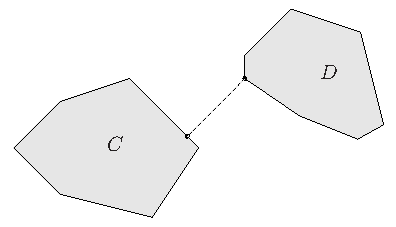
\includegraphics[width=.48\textwidth]{figures/ch08-417.pdf}
\caption*{图8.2 多面体 $C,D$ 之间的欧氏距离。虚线连接分别属于 $C,D$、欧氏距离最近的两个点。这两点可通过求解 QP 找到。}
\end{figure}
\subsubsection*{多面体之间的欧氏距离}
设多面体 $C,D$ 分别由线性不等式组 $A_1x\preceq b_1$、$A_2x\preceq b_2$ 描述。二者之间的距离，是分别属于 $C,D$ 的最近一对点的距离，见图8.2。这个距离是下列问题的最优值：
\begin{equation}\begin{array}{ll}\text{最小化}&\norm{x-y}_2\\\text{约束为}&A_1x\preceq b_1,\\&A_2y\preceq b_2.\end{array}\tag{8.4}\end{equation}
把目标平方，可以得到等价的 QP。
\subsection{分离凸集}
寻找两个凸集之间距离的问题(8.3)，其对偶通过集合之间的分离超平面具有有趣的几何解释。先将问题写成如下等价形式：
\begin{equation}\begin{array}{ll}\text{最小化}&\norm w\\\text{约束为}&f_i(x)\leq0,\quad i=1,\ldots,m,\\&g_i(y)\leq0,\quad i=1,\ldots,p,\\&x-y=w.\end{array}\tag{8.5}\end{equation}
对偶函数为
\[
 g(\lambda,z,\mu)=\inf_{x,y,w}\left(\norm w+\sum_{i=1}^m\lambda_if_i(x)
 +\sum_{i=1}^p\mu_ig_i(y)+z^\T(x-y-w)\right)
\]
% Source PDF page 418 (printed p. 404)
\[=\begin{cases}
 \displaystyle\inf_x\left(\sum_{i=1}^m\lambda_if_i(x)+z^\T x\right)
 +\inf_y\left(\sum_{i=1}^p\mu_ig_i(y)-z^\T y\right),&\norm z_*\leq1,\\
 -\infty,&\text{其他情况}.
\end{cases}\]
由此得到对偶问题
\begin{equation}\begin{array}{ll}
\text{最大化}&\displaystyle\inf_x\left(\sum_{i=1}^m\lambda_if_i(x)+z^\T x\right)
+\inf_y\left(\sum_{i=1}^p\mu_ig_i(y)-z^\T y\right)\\
\text{约束为}&\norm z_*\leq1,\\&\lambda\succeq0,\quad\mu\succeq0.
\end{array}\tag{8.6}\end{equation}
其几何解释如下。若 $\lambda,\mu$ 对偶可行且目标为正，则对所有 $x,y$ 有
\[\sum_{i=1}^m\lambda_if_i(x)+z^\T x+\sum_{i=1}^p\mu_ig_i(y)-z^\T y>0.\]
特别地，对 $x\in C$、$y\in D$，有 $z^\T x-z^\T y>0$，因此 $z$ 确定一个严格分离 $C,D$ 的超平面。

因此，若问题(8.5)与(8.6)之间强对偶成立，例如问题(8.5)严格可行，就有如下结论：若两个集合之间距离为正，就能用超平面将它们严格分离。
\subsubsection*{分离多面体}
对由线性不等式 $A_1x\preceq b_1$、$A_2x\preceq b_2$ 定义的集合应用这些对偶结果，得到对偶问题
\[\begin{array}{ll}
\text{最大化}&-b_1^\T\lambda-b_2^\T\mu\\
\text{约束为}&A_1^\T\lambda+z=0,\\&A_2^\T\mu-z=0,\\&\norm z_*\leq1,\\&\lambda\succeq0,\quad\mu\succeq0.
\end{array}\]
若 $\lambda,\mu,z$ 对偶可行，则对所有 $x\in C$、$y\in D$，
\[z^\T x=-\lambda^\T A_1x\geq-\lambda^\T b_1,\qquad
 z^\T y=\mu^\T A_2x\leq\mu^\T b_2,\]
若对偶目标为正，则
\[z^\T x-z^\T y\geq-\lambda^\T b_1-\mu^\T b_2>0,\]
即 $z$ 确定一个分离超平面。
\subsection{用示性函数与支撑函数表示距离和分离}
8.2.1节和8.2.2节的思路，可以用示性函数与支撑函数紧凑地表达。求两个凸集之间距离的问题可以写为
\[\begin{array}{ll}\text{最小化}&\norm{x-y}\\\text{约束为}&I_C(x)\leq0,\\&I_D(y)\leq0,\end{array}\]
% Source PDF page 419 (printed p. 405)
等价于
\[\begin{array}{ll}\text{最小化}&\norm w\\\text{约束为}&I_C(x)\leq0,\\&I_D(y)\leq0,\\&x-y=w.\end{array}\]
其对偶问题为
\[\begin{array}{ll}\text{最大化}&-S_C(-z)-S_D(z)\\\text{约束为}&\norm z_*\leq1.\end{array}\]
若 $z$ 对偶可行且目标为正，则 $S_D(z)<-S_C(-z)$，即
\[\sup_{x\in D}z^\T x<\inf_{x\in C}z^\T x.\]
也就是说，$z$ 确定一个严格分离 $C,D$ 的超平面。
\section{欧氏距离与角度问题}
设 $a_1,\ldots,a_n$ 是 $\R^n$ 中一组向量，暂且假设欧氏长度已知：
\[l_1=\norm{a_1}_2,\qquad\ldots,\qquad l_n=\norm{a_n}_2.\]
称这组向量为一个构形；若它们线性无关，则称为一组基。本节考虑涉及构形各种几何性质的优化问题，例如向量对之间的欧氏距离、夹角，以及刻画基的条件状况的各种几何指标。
\subsection{Gram 矩阵与可实现性}
长度、距离和角度都可以用向量 $a_1,\ldots,a_n$ 的 Gram 矩阵表示：
\[G=A^\T A,\qquad A=\begin{bmatrix}a_1&\cdots&a_n\end{bmatrix},\]
所以 $G_{ij}=a_i^\T a_j$。$G$ 的对角元为
\[G_{ii}=l_i^2,\qquad i=1,\ldots,n,\]
暂且假设它们已知且固定。$a_i$ 与 $a_j$ 之间的距离 $d_{ij}$ 为
\[\begin{aligned}
 d_{ij}&=\norm{a_i-a_j}_2\\
 &=(l_i^2+l_j^2-2a_i^\T a_j)^{1/2}\\
 &=(l_i^2+l_j^2-2G_{ij})^{1/2}.
\end{aligned}\]
% Source PDF page 420 (printed p. 406)
反过来，可以用 $d_{ij}$ 表示 $G_{ij}$：
\[G_{ij}=\frac{l_i^2+l_j^2-d_{ij}^2}2.\]
为后面引用，注意它是 $d_{ij}^2$ 的仿射函数。

非零向量 $a_i,a_j$ 之间的相关系数 $\rho_{ij}$ 为
\[\rho_{ij}=\frac{a_i^\T a_j}{\norm{a_i}_2\norm{a_j}_2}=\frac{G_{ij}}{l_il_j},\]
所以 $G_{ij}=l_il_j\rho_{ij}$ 是 $\rho_{ij}$ 的线性函数。非零向量 $a_i,a_j$ 之间的角度 $\theta_{ij}$ 为
\[\theta_{ij}=\cos^{-1}\rho_{ij}=\cos^{-1}(G_{ij}/(l_il_j)),\]
其中取 $\cos^{-1}\rho\in[0,\pi]$。因此 $G_{ij}=l_il_j\cos\theta_{ij}$。

长度、距离和角度在正交变换下保持不变：若 $Q\in\R^{n\times n}$ 正交，则向量组 $Qa_i,\ldots,Qa_n$ 具有相同的 Gram 矩阵，因而具有相同的长度、距离和角度。
\subsubsection*{可实现性}
Gram 矩阵 $G=A^\T A$ 当然对称且半正定。逆命题是线性代数的基本结论：矩阵 $G\in\mathbb S^n$ 是某组向量 $a_1,\ldots,a_n$ 的 Gram 矩阵，当且仅当 $G\succeq0$。当 $G\succeq0$ 时，求一个满足 $A^\T A=G$ 的矩阵 $A$，就能构造 Gram 矩阵为 $G$ 的构形。一个解是对称平方根 $A=G^{1/2}$。当 $G\succ0$ 时，可以通过 Cholesky 分解找到解：若 $LL^\T=G$，可取 $A=L^\T$。此外，给定任意一个解 $A$ 后，通过正交变换就能构造指定 Gram 矩阵 $G$ 的全部构形：若 $\widetilde A^\T\widetilde A=G$ 是任意解，则对某个正交矩阵 $Q$ 有 $\widetilde A=QA$。

因此，一组长度、距离和角度（或相关系数）可以实现，即来自某个构形，当且仅当相关 Gram 矩阵 $G$ 半正定，且对角元为 $l_1^2,\ldots,l_n^2$。

利用这一事实，可以把几个几何问题表示为凸优化问题，优化变量为 $G\in\mathbb S^n$。可实现性要求约束 $G\succeq0$ 以及 $G_{ii}=l_i^2$，$i=1,\ldots,n$。下面列出其他一些凸约束和目标。
\subsubsection*{角度与距离约束}
用线性等式约束 $G_{ij}=l_il_j\cos\alpha$，可以把角度固定为指定值 $\theta_{ij}=\alpha$。更一般地，用约束
\[l_il_j\cos\alpha\geq G_{ij}\geq l_il_j\cos\beta\]
可以规定角度的上下界 $\alpha\leq\theta_{ij}\leq\beta$，这是一对关于 $G$ 的线性不等式。这里使用了 $\cos^{-1}$ 单调递减。通过最小化或最大化 $G_{ij}$，也可以最大化或最小化某个角度 $\theta_{ij}$，同样利用了 $\cos^{-1}$ 的单调性。
% Source PDF page 421 (printed p. 407)
类似地也可以约束距离。要求 $d_{ij}$ 落在一个区间内，可用
\[\begin{aligned}
 d_{\min}\leq d_{ij}\leq d_{\max}
 &\Longleftrightarrow d_{\min}^2\leq d_{ij}^2\leq d_{\max}^2\\
 &\Longleftrightarrow d_{\min}^2\leq l_i^2+l_j^2-2G_{ij}\leq d_{\max}^2,
\end{aligned}\]
这是一对关于 $G$ 的线性不等式。通过最小化或最大化距离的平方，即 $G$ 的仿射函数，可以最小化或最大化距离本身。

例如，给定某些角度和某些距离的范围，即可能值的区间。通过求解两个 SDP，就能在所有构形上，找到另一个角度或另一个距离的最小、最大可能值。对最优 Gram 矩阵分解，可以重建对应的两个极端构形。
\subsubsection*{奇异值与条件数约束}
$A$ 的奇异值 $\sigma_1\geq\cdots\geq\sigma_n$ 是 $G$ 的特征值 $\lambda_1\geq\cdots\geq\lambda_n$ 的平方根。因此，$\sigma_1^2$ 是 $G$ 的凸函数，$\sigma_n^2$ 是 $G$ 的凹函数。于是，可以给 $A$ 的最大奇异值规定上界，或者将它最小化；可以给最小奇异值规定下界，或者将它最大化。$A$ 的条件数 $\sigma_1/\sigma_n$ 是 $G$ 的拟凸函数，因此可以通过拟凸优化，在满足其他几何约束的所有构形中，限制其最大允许值或将它最小化。

粗略地说，能够作为 $G$ 的凸约束施加的条件，是要求 $a_1,\ldots,a_n$ 构成条件良好的基的那些条件。
\subsubsection*{对偶基}
当 $G\succ0$ 时，$a_1,\ldots,a_n$ 构成 $\R^n$ 的一组基。对应的对偶基为 $b_1,\ldots,b_n$，满足
\[b_i^\T a_j=\begin{cases}1,&i=j,\\0,&i\ne j.\end{cases}\]
对偶基向量 $b_1,\ldots,b_n$ 就是矩阵 $A^{-1}$ 的各行。因此，对偶基的 Gram 矩阵为 $G^{-1}$。

可以把对偶基的几种几何条件写成关于 $G$ 的凸约束。对偶基向量长度的平方
\[\norm{b_i}_2^2=e_i^\T G^{-1}e_i\]
是 $G$ 的凸函数，因此可被最小化。$G^{-1}$ 的迹也是 $G$ 的凸函数，给出对偶基各向量长度平方之和，也是衡量基条件好坏的另一指标。
\subsubsection*{椭球与单纯形的体积}
椭球 $\{Au\mid\norm u_2\leq1\}$ 的体积也能衡量基的条件好坏，它为
\[\gamma(\det(A^\T A))^{1/2}=\gamma(\det G)^{1/2},\]
% Source PDF page 422 (printed p. 408)
其中 $\gamma$ 为 $\R^n$ 中单位球的体积。因此，对数体积为 $\log\gamma+\tfrac12\log\det G$，是 $G$ 的凹函数。于是，在凸的构形集合上最大化映像椭球的体积，可通过最大化 $\log\det G$ 完成。

对 $\R^n$ 中任意集合，结论相同：在 $A$ 下的像的体积，等于原体积乘以 $(\det G)^{1/2}$。例如，单位单纯形 $\conv\{0,e_1,\ldots,e_n\}$ 在 $A$ 下的像，是单纯形 $\conv\{0,a_1,\ldots,a_n\}$。其体积为 $\gamma(\det G)^{1/2}$，其中 $\gamma$ 为 $\R^n$ 中单位单纯形的体积。最大化 $\log\det G$，就能最大化这个单纯形的体积。
\subsection{只涉及角度的问题}
若只关心向量之间的角度或相关系数，不指定向量长度或彼此距离，直觉上只需假设各向量 $a_i$ 的长度 $l_i=1$。这很容易验证：Gram 矩阵具有形式 $G=\diag(l)C\diag(l)$，其中 $l$ 是长度向量，$C$ 为相关矩阵，即 $C_{ij}=\cos\theta_{ij}$。因此，若对某组正长度有 $G\succeq0$，则对任意一组正长度都有 $G\succeq0$；特别地，这当且仅当 $C\succeq0$，也就是假设所有长度均为一的情形。因此，一组角度 $\theta_{ij}\in[0,\pi]$、$i,j=1,\ldots,n$ 可实现，当且仅当 $C\succeq0$，这是关于相关系数的线性矩阵不等式。

例如，给定某些角度的上下界，等价于给某些相关系数规定上下界。通过求解两个 SDP，就能在全部构形中找到另一个角度的最小、最大可能值。
\begin{origexample}{8.3}
\textbf{相关系数的界。}考虑 $\R^4$ 中的例子，给定
\begin{equation}\begin{aligned}
 0.6\leq\rho_{12}\leq0.9,\qquad&0.8\leq\rho_{13}\leq0.9,\\
 0.5\leq\rho_{24}\leq0.7,\qquad&-0.8\leq\rho_{34}\leq-0.4.
\end{aligned}\tag{8.7}\end{equation}
为求 $\rho_{14}$ 的最小、最大可能值，求解两个 SDP：
\[\begin{array}{ll}
 \text{最小化／最大化}&\rho_{14}\\
 \text{约束为}&\text{式(8.7)},\\
 &\begin{bmatrix}1&\rho_{12}&\rho_{13}&\rho_{14}\\
 \rho_{12}&1&\rho_{23}&\rho_{24}\\
 \rho_{13}&\rho_{23}&1&\rho_{34}\\
 \rho_{14}&\rho_{24}&\rho_{34}&1\end{bmatrix}\succeq0,
\end{array}\]
变量为 $\rho_{12},\rho_{13},\rho_{14},\rho_{23},\rho_{24},\rho_{34}$。最小值、最大值取两位有效数字，分别为 $-0.39$ 和 $0.23$，对应的相关矩阵为
\[
 \begin{bmatrix}1.00&0.60&0.87&-0.39\\0.60&1.00&0.33&0.50\\0.87&0.33&1.00&-0.55\\-0.39&0.50&-0.55&1.00\end{bmatrix},\qquad
 \begin{bmatrix}1.00&0.71&0.80&0.23\\0.71&1.00&0.31&0.59\\0.80&0.31&1.00&-0.40\\0.23&0.59&-0.40&1.00\end{bmatrix}.
\]
\end{origexample}
% Source PDF page 423 (printed p. 409)
\subsection{欧氏距离问题}
在欧氏距离问题中，只关心向量之间的距离 $d_{ij}$，不关心向量的长度及其夹角。这些距离当然在正交变换下不变，而且在平移下也不变：对任意 $b\in\R^n$，构形 $\widetilde a_1=a_1+b,\ldots,\widetilde a_n=a_n+b$ 具有与原构形相同的距离。特别地，取
\[b=-\frac1n\sum_{i=1}^n a_i=-\frac1n A\one,\]
则 $\widetilde a_i$ 既保留原构形的距离，又满足 $\sum_{i=1}^n\widetilde a_i=0$。因此，在欧氏距离问题中，可以不失一般性地假设 $a_1,\ldots,a_n$ 的平均值为零，即 $A\one=0$。

求解欧氏距离问题时，可以把向量长度作为优化问题中的自由变量，这些长度本身不能出现在该类问题的目标或约束中。这里利用了如下事实：存在距离为 $d_{ij}\geq0$ 的构形，当且仅当存在长度 $l_1,\ldots,l_n$ 使 $G\succeq0$，其中 $G_{ij}=(l_i^2+l_j^2-d_{ij}^2)/2$。

定义 $z\in\R^n$、$z_i=l_i^2$，以及 $D\in\mathbb S^n$、$D_{ij}=d_{ij}^2$，当然 $D_{ii}=0$。存在某组长度使 $G\succeq0$ 的条件可写为
\begin{equation}
 G=(z\one^\T+\one z^\T-D)/2\succeq0\quad\text{对某个 }z\succeq0,\tag{8.8}
\end{equation}
这是关于 $D,z$ 的 LMI。元素非负、对角元为零且满足式(8.8)的矩阵 $D\in\mathbb S^n$，称为欧氏距离矩阵。矩阵是欧氏距离矩阵，当且仅当其元素是某个构形中向量之间欧氏距离的平方。给定欧氏距离矩阵 $D$ 及对应的长度平方向量 $z$，可用上述方法重建具有指定两两距离的一个或全部构形。

事实上，条件(8.8)等价于更简单的条件：$D$ 在 $\one^\perp$ 上半负定，即
\[\begin{aligned}
 (8.8)&\Longleftrightarrow u^\T Du\leq0\text{ 对所有满足 }\one^\T u=0\text{ 的 }u\\
 &\Longleftrightarrow(I-\tfrac1n\one\one^\T)D(I-\tfrac1n\one\one^\T)\preceq0.
\end{aligned}\]
这个简单矩阵不等式，连同 $D_{ij}\geq0$、$D_{ii}=0$，就是欧氏距离矩阵的经典刻画。为说明等价性，回顾可假设 $A\one=0$，从而 $\one^\T G\one=\one^\T A^\T A\one=0$。因此，$G\succeq0$ 当且仅当 $G$ 在 $\one^\perp$ 上半正定，即
\[\begin{aligned}
0&\preceq(I-\tfrac1n\one\one^\T)G(I-\tfrac1n\one\one^\T)\\
 &=\tfrac12(I-\tfrac1n\one\one^\T)(z\one^\T+\one z^\T-D)(I-\tfrac1n\one\one^\T)\\
 &=-\tfrac12(I-\tfrac1n\one\one^\T)D(I-\tfrac1n\one\one^\T),
\end{aligned}\]
即所需的简化条件。
% Source PDF page 424 (printed p. 410)
总之，矩阵 $D\in\mathbb S^n$ 是欧氏距离矩阵，即给出 $\R^n$ 中一组 $n$ 个向量之间的距离平方，当且仅当
\[D_{ii}=0,\quad i=1,\ldots,n,\qquad D_{ij}\geq0,\quad i,j=1,\ldots,n,\]
\[(I-\tfrac1n\one\one^\T)D(I-\tfrac1n\one\one^\T)\preceq0,\]
这是一组关于 $D$ 的线性等式、线性不等式以及矩阵不等式。因此，凡是关于距离平方凸的欧氏距离问题，都能表示为以 $D\in\mathbb S^n$ 为变量的凸问题。
\section{极值体积椭球}
设 $C\subseteq\R^n$ 有界且内部非空。本节考虑寻找位于 $C$ 内部的最大体积椭球，以及覆盖 $C$ 的最小体积椭球。这两个问题都能写成凸规划，但只有特殊情况下可有效求解。
\subsection{Löwner--John 椭球}
包含集合 $C$ 的最小体积椭球，称为 $C$ 的 Löwner--John 椭球，记为 $\mathcal E_{\mathrm{lj}}$。为刻画它，采用如下方式参数化一般椭球较为方便：
\begin{equation}\mathcal E=\{v\mid\norm{Av+b}_2\leq1\},\tag{8.9}\end{equation}
即欧氏单位球在仿射映射下的逆像。可以不失一般性地假设 $A\in\mathbb S_{++}^n$，此时 $\mathcal E$ 的体积正比于 $\det A^{-1}$。计算包含 $C$ 的最小体积椭球的问题可写为
\begin{equation}\begin{array}{ll}\text{最小化}&\log\det A^{-1}\\\text{约束为}&\sup_{v\in C}\norm{Av+b}_2\leq1,\end{array}\tag{8.10}\end{equation}
变量为 $A\in\mathbb S^n$、$b\in\R^n$，另有隐式约束 $A\succ0$。目标与约束函数关于 $A,b$ 均凸，所以问题(8.10)凸。但计算约束函数涉及求解凸函数最大化问题，只有某些特殊情况下可有效求解。
\subsubsection*{覆盖有限集的最小体积椭球}
考虑包含有限集 $C=\{x_1,\ldots,x_m\}\subseteq\R^n$ 的最小体积椭球。椭球覆盖 $C$ 当且仅当覆盖其凸包，所以覆盖 $C$ 的最小体积椭球，与包含多面体 $\conv\{x_1,\ldots,x_m\}$ 的最小体积椭球相同。
% Source PDF page 425 (printed p. 411)
应用式(8.10)，可写为
\begin{equation}\begin{array}{ll}\text{最小化}&\log\det A^{-1}\\\text{约束为}&\norm{Ax_i+b}_2\leq1,\quad i=1,\ldots,m,\end{array}\tag{8.11}\end{equation}
变量为 $A\in\mathbb S^n$、$b\in\R^n$，并有隐式约束 $A\succ0$。范数约束 $\norm{Ax_i+b}_2\leq1$ 关于 $A,b$ 是凸不等式。也可将其替换为平方形式 $\norm{Ax_i+b}_2^2\leq1$，这是关于 $A,b$ 的凸二次不等式。
\subsubsection*{覆盖椭球之并的最小体积椭球}
对于一些由二次不等式定义的集合 $C$，也能高效计算最小体积覆盖椭球。特别地，可以计算椭球的并集或和集的 Löwner--John 椭球。

例如，考虑寻找包含椭球 $\mathcal E_1,\ldots,\mathcal E_m$，从而包含它们并集的凸包，的最小体积椭球 $\mathcal E_{\mathrm{lj}}$。用凸二次不等式描述各椭球：
\[\mathcal E_i=\{x\mid x^\T A_ix+2b_i^\T x+c_i\leq0\},\qquad i=1,\ldots,m,\]
其中 $A_i\in\mathbb S_{++}^n$。将 $\mathcal E_{\mathrm{lj}}$ 参数化为
\[\begin{aligned}
 \mathcal E_{\mathrm{lj}}&=\{x\mid\norm{Ax+b}_2\leq1\}\\
 &=\{x\mid x^\T A^\T Ax+2(A^\T b)^\T x+b^\T b-1\leq0\},
\end{aligned}\]
其中 $A\in\mathbb S^n$、$b\in\R^n$。利用B.2节的结论，$\mathcal E_i\subseteq\mathcal E_{\mathrm{lj}}$ 当且仅当存在 $\tau\geq0$ 使
\[\begin{bmatrix}A^2-\tau A_i&Ab-\tau b_i\\(Ab-\tau b_i)^\T&b^\T b-1-\tau c_i\end{bmatrix}\preceq0.\]
$\mathcal E_{\mathrm{lj}}$ 的体积正比于 $\det A^{-1}$，因此求解
\[\begin{array}{ll}
\text{最小化}&\log\det A^{-1}\\
\text{约束为}&\tau_1\geq0,\ldots,\tau_m\geq0,\\
 &\begin{bmatrix}A^2-\tau_i A_i&Ab-\tau_i b_i\\(Ab-\tau_i b_i)^\T&b^\T b-1-\tau_i c_i\end{bmatrix}\preceq0,\quad i=1,\ldots,m,
\end{array}\]
可得包含全部椭球的最小体积椭球。或者，将变量 $b$ 替换为 $\widetilde b=Ab$，得到
\[\begin{array}{ll}
\text{最小化}&\log\det A^{-1}\\
\text{约束为}&\tau_1\geq0,\ldots,\tau_m\geq0,\\
 &\begin{bmatrix}
 A^2-\tau_i A_i&\widetilde b-\tau_i b_i&0\\
 (\widetilde b-\tau_i b_i)^\T&-1-\tau_i c_i&\widetilde b^\T\\
 0&\widetilde b&-A^2
 \end{bmatrix}\preceq0,\quad i=1,\ldots,m.
\end{array}\]
它关于变量 $A^2\in\mathbb S^n$、$\widetilde b$、$\tau_1,\ldots,\tau_m$ 凸。
% Source PDF page 426 (printed p. 412)
\begin{figure}[htbp]\centering
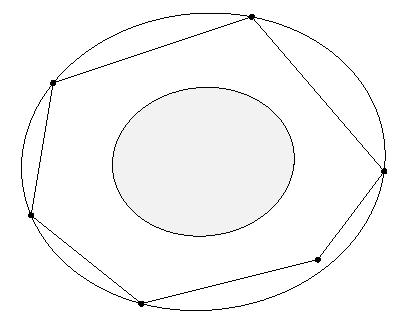
\includegraphics[width=.5\textwidth]{figures/ch08-426.pdf}
\caption*{图8.3 外侧椭圆是 Löwner--John 椭球的边界，即包围点 $x_1,\ldots,x_6$（图中的圆点），从而包围多面体 $P=\conv\{x_1,\ldots,x_6\}$ 的最小体积椭球。较小的椭圆是该椭球围绕中心缩小 $n=2$ 倍后的边界。缩小后的椭球保证位于 $P$ 内。}
\end{figure}
\subsubsection*{Löwner--John 椭球近似的效率}
设 $\mathcal E_{\mathrm{lj}}$ 为有界且内部非空的凸集 $C\subseteq\R^n$ 的 Löwner--John 椭球，中心为 $x_0$。若将该椭球围绕中心缩小 $n$ 倍，则所得椭球位于 $C$ 内：
\[x_0+\tfrac1n(\mathcal E_{\mathrm{lj}}-x_0)\subseteq C\subseteq\mathcal E_{\mathrm{lj}}.\]
换句话说，Löwner--John 椭球能够近似任意凸集，其因子只依赖于维数 $n$。图8.3给出一个简单例子。

若不对 $C$ 作额外假设，因子 $1/n$ 无法改进。例如，$\R^n$ 中任意单纯形的 Löwner--John 椭球都必须缩小 $n$ 倍才能放入其中，见习题8.13。

下面对特殊情况 $C=\conv\{x_1,\ldots,x_m\}$ 证明这一效率结论。将式(8.11)中的范数约束平方，引入 $\widetilde A=A^2$ 和 $\widetilde b=Ab$，得到
\begin{equation}\begin{array}{ll}
\text{最小化}&\log\det\widetilde A^{-1}\\
\text{约束为}&x_i^\T\widetilde A x_i-2\widetilde b^\T x_i+\widetilde b^\T\widetilde A^{-1}\widetilde b\leq1,\quad i=1,\ldots,m.
\end{array}\tag{8.12}\end{equation}
其 KKT 条件为
\[\begin{gathered}
 \sum_{i=1}^m\lambda_i(x_ix_i^\T-\widetilde A^{-1}\widetilde b\widetilde b^\T\widetilde A^{-1})=\widetilde A^{-1},\qquad
 \sum_{i=1}^m\lambda_i(x_i-\widetilde A^{-1}\widetilde b)=0,\\
 \lambda_i\geq0,\quad
 x_i^\T\widetilde A x_i-2\widetilde b^\T x_i+\widetilde b^\T\widetilde A^{-1}\widetilde b\leq1,\quad i=1,\ldots,m,\\
 \lambda_i(1-x_i^\T\widetilde A x_i+2\widetilde b^\T x_i-\widetilde b^\T\widetilde A^{-1}\widetilde b)=0,\quad i=1,\ldots,m.
\end{gathered}\]
通过适当的仿射坐标变换，可以假设 $\widetilde A=I$、$\widetilde b=0$，即最小体积椭球是以原点为中心的单位球。
% Source PDF page 427 (printed p. 413)
KKT 条件于是简化为
\[\sum_{i=1}^m\lambda_i x_ix_i^\T=I,\qquad
 \sum_{i=1}^m\lambda_i x_i=0,\qquad
 \lambda_i(1-x_i^\T x_i)=0,\quad i=1,\ldots,m,\]
再加上可行性条件 $\norm{x_i}_2\leq1$、$\lambda_i\geq0$。对第一个等式两边取迹并利用互补松弛，还得到 $\sum_{i=1}^m\lambda_i=n$。

在新坐标中，缩小后的椭球是以原点为中心、半径 $1/n$ 的球。需要证明
\[\norm x_2\leq1/n\ \Longrightarrow\ x\in C=\conv\{x_1,\ldots,x_m\}.\]
设 $\norm x_2\leq1/n$。由 KKT 条件可知
\begin{equation}
 x=\sum_{i=1}^m\lambda_i(x^\T x_i)x_i
 =\sum_{i=1}^m\lambda_i(x^\T x_i+1/n)x_i
 =\sum_{i=1}^m\mu_ix_i,\tag{8.13}
\end{equation}
其中 $\mu_i=\lambda_i(x^\T x_i+1/n)$。由 Cauchy--Schwarz 不等式，
\[\mu_i=\lambda_i(x^\T x_i+1/n)\geq\lambda_i(-\norm x_2\norm{x_i}_2+1/n)
 \geq\lambda_i(-1/n+1/n)=0.\]
此外，
\[\sum_{i=1}^m\mu_i=\sum_{i=1}^m\lambda_i(x^\T x_i+1/n)=\sum_{i=1}^m\lambda_i/n=1.\]
结合式(8.13)，说明 $x$ 是 $x_1,\ldots,x_m$ 的凸组合，从而 $x\in C$。
\subsubsection*{对称集的 Löwner--John 椭球近似效率}
若集合 $C$ 关于某点 $x_0$ 对称，则因子 $1/n$ 可以改进为 $1/\sqrt n$：
\[x_0+\tfrac1{\sqrt n}(\mathcal E_{\mathrm{lj}}-x_0)\subseteq C\subseteq\mathcal E_{\mathrm{lj}}.\]
因子 $1/\sqrt n$ 同样是紧的。立方体
\[C=\{x\in\R^n\mid-\one\preceq x\preceq\one\}\]
的 Löwner--John 椭球是半径 $\sqrt n$ 的球。将其缩小 $\sqrt n$ 倍，得到包含在 $C$ 中、并在 $x=\pm e_i$ 处与边界相切的球。
\subsubsection*{用二次范数近似范数}
设 $\norm{\cdot}$ 是 $\R^n$ 上任意范数，$C=\{x\mid\norm x\leq1\}$ 是其单位球。设 $\mathcal E_{\mathrm{lj}}=\{x\mid x^\T Ax\leq1\}$、$A\in\mathbb S_{++}^n$ 是 $C$ 的 Löwner--John 椭球。由于 $C$ 关于原点对称，上述结果说明 $(1/\sqrt n)\mathcal E_{\mathrm{lj}}\subseteq C\subseteq\mathcal E_{\mathrm{lj}}$。

用 $\norm{\cdot}_{\mathrm{lj}}$ 表示二次范数
\[\norm z_{\mathrm{lj}}=(z^\T Az)^{1/2},\]
% Source PDF page 428 (printed p. 414)
其单位球为 $\mathcal E_{\mathrm{lj}}$。包含关系 $(1/\sqrt n)\mathcal E_{\mathrm{lj}}\subseteq C\subseteq\mathcal E_{\mathrm{lj}}$ 等价于对所有 $z\in\R^n$ 的不等式
\[\norm z_{\mathrm{lj}}\leq\norm z\leq\sqrt n\norm z_{\mathrm{lj}}.\]
换句话说，二次范数 $\norm{\cdot}_{\mathrm{lj}}$ 在 $\sqrt n$ 因子内近似范数 $\norm{\cdot}$。特别地，$\R^n$ 上任意范数都可以由二次范数在 $\sqrt n$ 因子内近似。
\subsection{最大体积内接椭球}
现在考虑寻找位于凸集 $C$ 内的最大体积椭球，其中假设 $C$ 有界且内部非空。为建立模型，将椭球参数化为单位球在仿射变换下的像，即
\[\mathcal E=\{Bu+d\mid\norm u_2\leq1\}.\]
仍可以假设 $B\in\mathbb S_{++}^n$，体积因而正比于 $\det B$。求解凸优化问题
\begin{equation}\begin{array}{ll}
\text{最大化}&\log\det B\\
\text{约束为}&\sup_{\norm u_2\leq1} I_C(Bu+d)\leq0
\end{array}\tag{8.14}\end{equation}
即可求得 $C$ 内的最大体积椭球，变量为 $B\in\mathbb S^n$、$d\in\R^n$，隐式约束为 $B\succ0$。
\subsubsection*{多面体中的最大体积椭球}
考虑 $C$ 是由线性不等式组描述的多面体：
\[C=\{x\mid a_i^\T x\leq b_i,\ i=1,\ldots,m\}.\]
为应用式(8.14)，先把约束改写为更方便的形式：
\[\begin{aligned}
 \sup_{\norm u_2\leq1}I_C(Bu+d)\leq0
 &\Longleftrightarrow\sup_{\norm u_2\leq1}a_i^\T(Bu+d)\leq b_i,\quad i=1,\ldots,m\\
 &\Longleftrightarrow\norm{Ba_i}_2+a_i^\T d\leq b_i,\quad i=1,\ldots,m.
\end{aligned}\]
于是将式(8.14)表示为关于变量 $B,d$ 的凸优化问题：
\begin{equation}\begin{array}{ll}\text{最小化}&\log\det B^{-1}\\\text{约束为}&\norm{Ba_i}_2+a_i^\T d\leq b_i,\quad i=1,\ldots,m.\end{array}\tag{8.15}\end{equation}
\subsubsection*{椭球交集中的最大体积椭球}
也可以寻找位于 $m$ 个椭球 $\mathcal E_1,\ldots,\mathcal E_m$ 交集内的最大体积椭球 $\mathcal E$。用 $\mathcal E=\{Bu+d\mid\norm u_2\leq1\}$、$B\in\mathbb S_{++}^n$ 描述它；其他椭球用凸二次不等式描述：
\[\mathcal E_i=\{x\mid x^\T A_ix+2b_i^\T x+c_i\leq0\},\quad i=1,\ldots,m,\]
% Source PDF page 429 (printed p. 415)
其中 $A_i\in\mathbb S_{++}^n$。先求出 $\mathcal E\subseteq\mathcal E_i$ 的条件。这当且仅当
\[\begin{aligned}
 &\sup_{\norm u_2\leq1}\bigl((d+Bu)^\T A_i(d+Bu)+2b_i^\T(d+Bu)+c_i\bigr)\\
 &\quad=d^\T A_id+2b_i^\T d+c_i
 +\sup_{\norm u_2\leq1}\bigl(u^\T BA_iBu+2(A_id+b_i)^\T Bu\bigr)\leq0.
\end{aligned}\]
根据B.1节，
\[\sup_{\norm u_2\leq1}\bigl(u^\T BA_iBu+2(A_id+b_i)^\T Bu\bigr)
 \leq-(d^\T A_id+2b_i^\T d+c_i)\]
当且仅当存在 $\lambda_i\geq0$ 使
\[\begin{bmatrix}
 -\lambda_i-d^\T A_id-2b_i^\T d-c_i&(A_id+b_i)^\T B\\
 B(A_id+b_i)&\lambda_i I-BA_iB
\end{bmatrix}\succeq0.\]
因此，求解
\[\begin{array}{ll}
\text{最小化}&\log\det B^{-1}\\
\text{约束为}&\begin{bmatrix}
 -\lambda_i-d^\T A_id-2b_i^\T d-c_i&(A_id+b_i)^\T B\\
 B(A_id+b_i)&\lambda_i I-BA_iB
\end{bmatrix}\succeq0,\quad i=1,\ldots,m,
\end{array}\]
可求得包含在 $\mathcal E_1,\ldots,\mathcal E_m$ 中的最大体积椭球，变量为 $B\in\mathbb S^n$、$d\in\R^n$、$\lambda\in\R^m$。等价地，求解
\[\begin{array}{ll}
\text{最小化}&\log\det B^{-1}\\
\text{约束为}&\begin{bmatrix}
 -\lambda_i-c_i+b_i^\T A_i^{-1}b_i&0&(d+A_i^{-1}b_i)^\T\\
 0&\lambda_i I&B\\
 d+A_i^{-1}b_i&B&A_i^{-1}
 \end{bmatrix}\succeq0,\quad i=1,\ldots,m.
\end{array}\]
\subsubsection*{椭球内近似的效率}
最大体积内接椭球也有与 Löwner--John 椭球类似的近似效率结论。若 $C\subseteq\R^n$ 凸、有界且内部非空，则将最大体积内接椭球围绕中心扩大 $n$ 倍，就能覆盖 $C$。若集合关于某点对称，因子 $n$ 可改进为 $\sqrt n$。图8.4给出一个例子。
\subsection{极值体积椭球的仿射不变性}
Löwner--John 椭球和最大体积内接椭球都具有仿射不变性。若 $\mathcal E_{\mathrm{lj}}$ 是 $C$ 的 Löwner--John 椭球，$T\in\R^{n\times n}$ 非奇异，则 $TC$ 的 Löwner--John 椭球是 $T\mathcal E_{\mathrm{lj}}$。最大体积内接椭球也有类似结论。

为证明这一结论，设 $\mathcal E$ 是任意覆盖 $C$ 的椭球，则 $T\mathcal E$ 覆盖 $TC$。反过来也成立：覆盖 $TC$ 的每个椭球都具有 $T\mathcal E$ 的形式，其中 $\mathcal E$ 覆盖 $C$。
% Source PDF page 430 (printed p. 416)
\begin{figure}[htbp]\centering
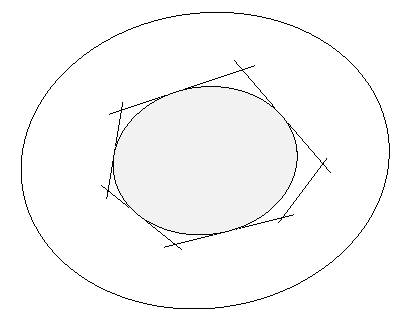
\includegraphics[width=.5\textwidth]{figures/ch08-430.pdf}
\caption*{图8.4 内接于多面体 $P$ 的最大体积椭球，以阴影表示。外侧椭圆是内椭球围绕中心扩大 $n=2$ 倍后的边界。扩大的椭球保证覆盖 $P$。}
\end{figure}
换句话说，关系 $\widetilde{\mathcal E}=T\mathcal E$ 建立了覆盖 $TC$ 的椭球与覆盖 $C$ 的椭球之间的一一对应。此外，对应椭球的体积之比都是 $|\det T|$，因此特别地，若 $\mathcal E$ 在覆盖 $C$ 的椭球中体积最小，则 $T\mathcal E$ 在覆盖 $TC$ 的椭球中体积最小。
\section{求中心}
\subsection{Chebyshev 中心}
设 $C\subseteq\R^n$ 有界、内部非空，$x\in C$。点 $x\in C$ 的深度定义为
\[\operatorname{depth}(x,C)=\dist(x,\R^n\setminus C),\]
即到 $C$ 外部最近点的距离。深度给出了以 $x$ 为中心、位于 $C$ 内的最大球的半径。集合 $C$ 的 Chebyshev 中心定义为 $C$ 中任意深度最大的点：
\[x_{\mathrm{cheb}}(C)=\argmax\operatorname{depth}(x,C)
 =\argmax\dist(x,\R^n\setminus C).\]
Chebyshev 中心是 $C$ 内离外部最远的点，也是位于 $C$ 内的最大球的中心。图8.5给出 $C$ 为多面体、范数为欧氏范数的例子。
% Source PDF page 431 (printed p. 417)
\begin{figure}[htbp]\centering
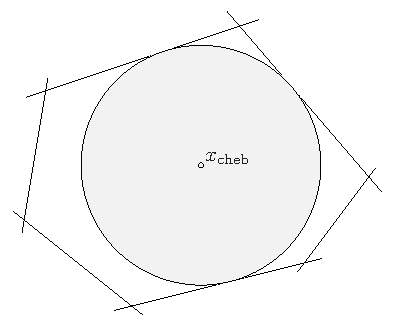
\includegraphics[width=.5\textwidth]{figures/ch08-431.pdf}
\caption*{图8.5 欧氏范数下多面体 $C$ 的 Chebyshev 中心。中心 $x_{\mathrm{cheb}}$ 是 $C$ 内最深的点，即离 $C$ 的外部或补集最远的点。它也是位于 $C$ 内的最大欧氏球（浅色阴影）的中心。}
\end{figure}
\subsubsection*{凸集的 Chebyshev 中心}
当集合 $C$ 凸时，深度是 $x\in C$ 的凹函数，因此计算 Chebyshev 中心是凸优化问题，见习题8.5。具体地，设 $C\subseteq\R^n$ 由一组凸不等式定义：
\[C=\{x\mid f_1(x)\leq0,\ldots,f_m(x)\leq0\}.\]
可通过求解问题
\begin{equation}\begin{array}{ll}\text{最大化}&R\\\text{约束为}&g_i(x,R)\leq0,\quad i=1,\ldots,m,\end{array}\tag{8.16}\end{equation}
找到 Chebyshev 中心，其中
\[g_i(x,R)=\sup_{\norm u\leq1}f_i(x+Ru).\]
问题(8.16)是凸优化问题，因为每个 $g_i$ 都是一族关于 $x,R$ 的凸函数的逐点最大值，因此凸。但计算 $g_i$ 需要以数值或解析方式求解凸函数最大化问题，这可能非常困难。实际中，只有 $g_i$ 容易计算时，才能求出 Chebyshev 中心。
\subsubsection*{多面体的 Chebyshev 中心}
设 $C$ 由线性不等式组 $a_i^\T x\leq b_i$、$i=1,\ldots,m$ 定义。当 $R\geq0$ 时有
\[g_i(x,R)=\sup_{\norm u\leq1}\bigl(a_i^\T(x+Ru)-b_i\bigr)
 =a_i^\T x+R\norm{a_i}_*-b_i.\]
% Source PDF page 432 (printed p. 418)
因此，求解 LP
\[\begin{array}{ll}\text{最大化}&R\\\text{约束为}&a_i^\T x+R\norm{a_i}_*\leq b_i,\quad i=1,\ldots,m,\\&R\geq0,\end{array}\]
即可得到 Chebyshev 中心，变量为 $x,R$。
\subsubsection*{椭球交集的欧氏 Chebyshev 中心}
设 $C$ 为 $m$ 个椭球的交，由二次不等式定义：
\[C=\{x\mid x^\T A_ix+2b_i^\T x+c_i\leq0,\ i=1,\ldots,m\},\]
其中 $A_i\in\mathbb S_{++}^n$。有
\[\begin{aligned}
 g_i(x,R)&=\sup_{\norm u_2\leq1}\bigl((x+Ru)^\T A_i(x+Ru)+2b_i^\T(x+Ru)+c_i\bigr)\\
 &=x^\T A_ix+2b_i^\T x+c_i
 +\sup_{\norm u_2\leq1}\bigl(R^2u^\T A_iu+2R(A_ix+b_i)^\T u\bigr).
\end{aligned}\]
由B.1节，$g_i(x,R)\leq0$ 当且仅当存在 $\lambda_i$ 使矩阵不等式
\begin{equation}\begin{bmatrix}
 -x^\T A_ix_i-2b_i^\T x-c_i-\lambda_i&R(A_ix+b_i)^\T\\
 R(A_ix+b_i)&\lambda_i I-R^2A_i
\end{bmatrix}\succeq0\tag{8.17}\end{equation}
成立。利用这一结论，可将 Chebyshev 中心问题写成
\[\begin{array}{ll}
\text{最大化}&R\\
\text{约束为}&\begin{bmatrix}
 -\lambda_i-c_i+b_i^\T A_i^{-1}b_i&0&(x+A_i^{-1}b_i)^\T\\
 0&\lambda_i I&RI\\
 x+A_i^{-1}b_i&RI&A_i^{-1}
 \end{bmatrix}\succeq0,\quad i=1,\ldots,m,
\end{array}\]
这是以 $R,\lambda,x$ 为变量的 SDP。LMI 约束中 $A_i^{-1}$ 的 Schur 补，恰为式(8.17)的左端。
\subsection{最大体积椭球中心}
集合 $C\subseteq\R^n$ 的 Chebyshev 中心 $x_{\mathrm{cheb}}$，是位于 $C$ 内的最大球的中心。推广这一想法，将 $C$ 的最大体积椭球中心 $x_{\mathrm{mve}}$ 定义为位于 $C$ 内的最大体积椭球的中心。图8.6给出 $C$ 为多面体的例子。

当 $C$ 由一组线性不等式定义时，求解问题(8.15)即可得到最大体积椭球中心，变量 $d\in\R^n$ 的最优值就是 $x_{\mathrm{mve}}$。由于 $C$ 内的最大体积椭球具有仿射不变性，最大体积椭球中心也具有仿射不变性。
% Source PDF page 433 (printed p. 419)
\begin{figure}[htbp]\centering
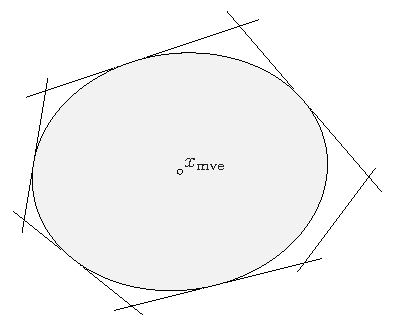
\includegraphics[width=.5\textwidth]{figures/ch08-433.pdf}
\caption*{图8.6 浅色阴影椭球为集合 $C$ 内的最大体积椭球，这里的 $C$ 与图8.5为同一个多面体。它的中心 $x_{\mathrm{mve}}$ 就是 $C$ 的最大体积椭球中心。}
\end{figure}
\subsection{不等式组的解析中心}
凸不等式与线性等式组
\[f_i(x)\leq0,\quad i=1,\ldots,m,\qquad Fx=g\]
的解析中心 $x_{\mathrm{ac}}$，定义为以下凸问题的一个最优点：
\begin{equation}\begin{array}{ll}\text{最小化}&-\sum_{i=1}^m\log(-f_i(x))\\\text{约束为}&Fx=g,\end{array}\tag{8.18}\end{equation}
变量为 $x\in\R^n$，隐式约束为 $f_i(x)<0$、$i=1,\ldots,m$。式(8.18)中的目标称为与该不等式组关联的对数障碍。这里假设对数障碍的定义域与等式定义的仿射集相交，即严格不等式组
\[f_i(x)<0,\quad i=1,\ldots,m,\qquad Fx=g\]
可行。若可行集
\[C=\{x\mid f_i(x)<0,\ i=1,\ldots,m,\ Fx=g\}\]
有界，则对数障碍在可行集上有下界。

当 $x$ 严格可行，即 $Fx=g$ 且各 $f_i(x)<0$ 时，可将 $-f_i(x)$ 理解为第 $i$ 条不等式的裕量或松弛量。解析中心 $x_{\mathrm{ac}}$ 是满足等式约束 $Fx=g$ 及隐式约束 $f_i(x)<0$，并使这些松弛量或裕量的乘积（或几何平均）最大的点。

解析中心不是由不等式与等式描述的集合 $C$ 的函数：两组不等式与等式可以定义同一个集合，却具有不同解析中心。尽管如此，人们仍常非正式地使用“集合 $C$ 的解析中心”，来指代定义该集合的某组等式与不等式的解析中心。
% Source PDF page 434 (printed p. 420)
不过，解析中心不依赖于仿射坐标变换。它也在不等式函数的正数缩放、以及等式约束的任意重新参数化下保持不变。换句话说，若 $\widetilde F,\widetilde g$ 使 $\widetilde Fx=\widetilde g$ 当且仅当 $Fx=g$，且 $\alpha_1,\ldots,\alpha_m>0$，则
\[\alpha_i f_i(x)\leq0,\quad i=1,\ldots,m,\qquad\widetilde Fx=\widetilde g\]
的解析中心，与
\[f_i(x)\leq0,\quad i=1,\ldots,m,\qquad Fx=g\]
的解析中心相同，见习题8.17。
\subsubsection*{线性不等式组的解析中心}
线性不等式组
\[a_i^\T x\leq b_i,\qquad i=1,\ldots,m\]
的解析中心是无约束最小化问题
\begin{equation}\text{最小化}\quad-\sum_{i=1}^m\log(b_i-a_i^\T x)\tag{8.19}\end{equation}
的解，隐式约束为 $b_i-a_i^\T x>0$、$i=1,\ldots,m$。若线性不等式定义的多面体有界，则对数障碍有下界且严格凸，因此解析中心唯一，见习题4.2。

线性不等式组的解析中心有一个几何解释。由于解析中心不依赖于约束函数的正数缩放，可以不失一般性地假设 $\norm{a_i}_2=1$。此时，松弛量 $b_i-a_i^\T x$ 是到超平面 $H_i=\{x\mid a_i^\T x=b_i\}$ 的距离。因此，解析中心 $x_{\mathrm{ac}}$ 使到各定义超平面距离的乘积最大。
\subsubsection*{由线性不等式解析中心得到的内、外椭球}
线性不等式组的解析中心，通过对数障碍函数
\[-\sum_{i=1}^m\log(b_i-a_i^\T x)\]
在解析中心处的 Hessian，隐式确定一个内接椭球和一个覆盖椭球。该 Hessian 为
\[H=\sum_{i=1}^m d_i^2a_ia_i^\T,\qquad
 d_i=\frac1{b_i-a_i^\T x_{\mathrm{ac}}},\quad i=1,\ldots,m.\]
有 $\mathcal E_{\mathrm{inner}}\subseteq P\subseteq\mathcal E_{\mathrm{outer}}$，其中
\[\begin{aligned}
P&=\{x\mid a_i^\T x\leq b_i,\ i=1,\ldots,m\},\\
\mathcal E_{\mathrm{inner}}&=\{x\mid(x-x_{\mathrm{ac}})^\T H(x-x_{\mathrm{ac}})\leq1\},\\
\mathcal E_{\mathrm{outer}}&=\{x\mid x-x_{\mathrm{ac}})^\T H(x-x_{\mathrm{ac}})\leq m(m-1)\}.
\end{aligned}\]
% Source PDF page 435 (printed p. 421)
\begin{figure}[htbp]\centering
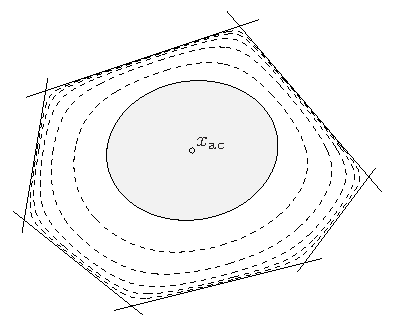
\includegraphics[width=.5\textwidth]{figures/ch08-435.pdf}
\caption*{图8.7 虚线为定义图8.5中多面体 $C$ 的不等式组所对应对数障碍函数的五条等高线。标为 $x_{\mathrm{ac}}$ 的对数障碍最小点，是不等式组的解析中心。内椭球 $\mathcal E_{\mathrm{inner}}=\{x\mid(x-x_{\mathrm{ac}})H(x-x_{\mathrm{ac}})\leq1\}$ 以阴影表示，其中 $H$ 为对数障碍在 $x_{\mathrm{ac}}$ 处的 Hessian。}
\end{figure}
这个结论比最大体积内接椭球的结论弱，后者扩大 $n$ 倍就覆盖多面体。对数障碍 Hessian 所定义的内、外椭球，其缩放因子为 $(m(m-1))^{1/2}$，总不小于 $n$。

为证明 $\mathcal E_{\mathrm{inner}}\subseteq P$，设 $x\in\mathcal E_{\mathrm{inner}}$，即
\[(x-x_{\mathrm{ac}})^\T H(x-x_{\mathrm{ac}})
 =\sum_{i=1}^m(d_i a_i^\T(x-x_{\mathrm{ac}}))^2\leq1.\]
这说明
\[a_i^\T(x-x_{\mathrm{ac}})\leq1/d_i=b_i-a_i^\T x_{\mathrm{ac}},\qquad i=1,\ldots,m,\]
所以对所有 $i$ 有 $a_i^\T x\leq b_i$。这里并未使用 $x_{\mathrm{ac}}$ 是解析中心，因此把 $x_{\mathrm{ac}}$ 换成任意严格可行点，结论仍成立。

为证明 $P\subseteq\mathcal E_{\mathrm{outer}}$，需要用到 $x_{\mathrm{ac}}$ 为解析中心这一事实，因此对数障碍梯度为零：
\[\sum_{i=1}^m d_ia_i=0.\]
现在假设 $x\in P$，则
\[\begin{aligned}
 (x-x_{\mathrm{ac}})^\T H(x-x_{\mathrm{ac}})
 &=\sum_{i=1}^m(d_i a_i^\T(x-x_{\mathrm{ac}}))^2\\
% Source PDF page 436 (printed p. 422)
 &=\sum_{i=1}^m d_i^2(1/d_i-a_i^\T(x-x_{\mathrm{ac}}))^2-m\\
 &=\sum_{i=1}^m d_i^2(b_i-a_i^\T x)^2-m\\
 &\leq\left(\sum_{i=1}^m d_i(b_i-a_i^\T x)\right)^2-m\\
 &=\left(\sum_{i=1}^m d_i(b_i-a_i^\T x_{\mathrm{ac}})
       +\sum_{i=1}^m d_i a_i^\T(x_{\mathrm{ac}}-x)\right)^2-m\\
 &=m^2-m,
\end{aligned}\]
表明 $x\in\mathcal E_{\mathrm{outer}}$。第二个等式来自 $\sum_{i=1}^m d_ia_i=0$；不等式来自对 $y\succeq0$ 成立的 $\sum_{i=1}^m y_i^2\leq(\sum_{i=1}^m y_i)^2$；最后一个等式使用了 $\sum_{i=1}^m d_ia_i=0$ 和 $d_i$ 的定义。
\subsubsection*{线性矩阵不等式的解析中心}
若在锥 $K$ 上定义对数，解析中心的定义就能推广到由相对于 $K$ 的广义不等式描述的集合。例如，线性矩阵不等式
\[x_1A_1+x_2A_2+\cdots+x_nA_n\preceq B\]
的解析中心，定义为
\[\text{最小化}\quad-\log\det(B-x_1A_1-\cdots-x_nA_n)\]
的解。
\section{分类}
在模式识别和分类问题中，给定 $\R^n$ 中两组点 $\{x_1,\ldots,x_N\}$、$\{y_1,\ldots,y_M\}$，希望在指定函数族中找到 $f:\R^n\to\R$，使它在第一组点上为正，在第二组点上为负，即
\[f(x_i)>0,\quad i=1,\ldots,N,\qquad f(y_i)<0,\quad i=1,\ldots,M.\]
若这些不等式成立，就说 $f$ 或其零水平集 $\{x\mid f(x)=0\}$ 分离、分类或判别了两组点。有时也考虑弱分离，即上述不等式取非严格形式。
% Source PDF page 437 (printed p. 423)
\begin{figure}[htbp]\centering
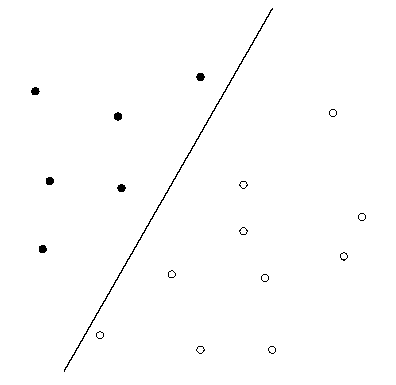
\includegraphics[width=.48\textwidth]{figures/ch08-437.pdf}
\caption*{图8.8 点 $x_1,\ldots,x_N$ 以空心圆表示，点 $y_1,\ldots,y_M$ 以实心圆表示。仿射函数 $f$ 对这两组点进行分类，它的零水平集是一条分离二者的直线。}
\end{figure}
\subsection{线性判别}
线性判别要寻找对点分类的仿射函数 $f(x)=a^\T x-b$，即
\begin{equation}a^\T x_i-b>0,\quad i=1,\ldots,N,\qquad
 a^\T y_i-b<0,\quad i=1,\ldots,M.\tag{8.20}\end{equation}
几何上，就是寻找分离两组点的超平面。由于严格不等式(8.20)关于 $a,b$ 齐次，它们可行当且仅当关于变量 $a,b$ 的非严格线性不等式组
\begin{equation}a^\T x_i-b\geq1,\quad i=1,\ldots,N,\qquad
 a^\T y_i-b\leq-1,\quad i=1,\ldots,M\tag{8.21}\end{equation}
可行。图8.8给出两组点与线性判别函数的一个简单例子。
\subsubsection*{线性判别的择一定理}
严格不等式组(8.20)的强择一条件，是存在 $\lambda,\widetilde\lambda$ 使
\begin{equation}\begin{gathered}
 \lambda\succeq0,\quad\widetilde\lambda\succeq0,\quad(\lambda,\widetilde\lambda)\ne0,\\
 \sum_{i=1}^N\lambda_ix_i=\sum_{i=1}^M\widetilde\lambda_i y_i,\qquad
 \one^\T\lambda=\one^\T\widetilde\lambda.
\end{gathered}\tag{8.22}\end{equation}
见5.8.3节。利用第三个和最后一个条件，可将择一条件写为
\[\lambda\succeq0,\quad\one^\T\lambda=1,\quad
 \widetilde\lambda\succeq0,\quad\one^\T\widetilde\lambda=1,\quad
 \sum_{i=1}^N\lambda_ix_i=\sum_{i=1}^M\widetilde\lambda_i y_i.\]
% Source PDF page 438 (printed p. 424)
这里除以正数 $\one^\T\lambda$，并沿用原符号表示归一化后的 $\lambda,\widetilde\lambda$。这些条件的几何含义很简单：存在一个点同时属于 $\{x_1,\ldots,x_N\}$ 与 $\{y_1,\ldots,y_M\}$ 的凸包。换句话说，两组点能够线性判别，即用仿射函数判别，当且仅当其凸包不相交。前面已多次遇到这一结论。
\subsubsection*{稳健线性判别}
存在仿射分类函数 $f(x)=a^\T x-b$，等价于定义该函数的变量 $a,b$ 满足一组线性不等式。若两组点可线性判别，则判别它们的仿射函数构成一个多面体，可以选择其中使某种稳健性指标最优的函数。例如，可以寻找在 $x_i$ 处的正值与 $y_i$ 处的负值之间具有最大可能间隔的函数。为此必须归一化 $a,b$，否则将二者乘以正常数就能使函数值间隔任意大。这导出问题
\begin{equation}\begin{array}{ll}
\text{最大化}&t\\
\text{约束为}&a^\T x_i-b\geq t,\quad i=1,\ldots,N,\\
&a^\T y_i-b\leq-t,\quad i=1,\ldots,M,\\
&\norm a_2\leq1,
\end{array}\tag{8.23}\end{equation}
变量为 $a,b,t$。这个凸问题具有线性目标、线性不等式以及一个二次不等式；其最优值 $t^\star$ 为正，当且仅当两组点可线性判别。此时，$\norm a_2\leq1$ 在最优点总取等号，即 $\norm{a^\star}_2=1$，见习题8.23。

稳健线性判别问题(8.23)有简单的几何解释。若 $\norm a_2=1$，任意最优点都满足这一点，则 $a^\T x_i-b$ 是 $x_i$ 到分离超平面 $H=\{z\mid a^\T z=b\}$ 的欧氏距离。同样，$b-a^\T y_i$ 为 $y_i$ 到该超平面的距离。因此，问题(8.23)寻找既分离两组点、又与它们距离最大的超平面。也就是说，它寻找能分离两组点的最厚平板。

如图8.9所示，最优值 $t^\star$，即平板厚度的一半，事实上等于两组点凸包之间距离的一半。这可从问题(8.23)的对偶清楚地看出。对最小化 $-t$ 的问题，拉格朗日函数为
\[-t+\sum_{i=1}^N u_i(t+b-a^\T x_i)
 +\sum_{i=1}^M v_i(t-b+a^\T y_i)+\lambda(\norm a_2-1).\]
对 $b,t$ 最小化，得到条件 $\one^\T u=1/2$、$\one^\T v=1/2$。这些条件成立时，
\[g(u,v,\lambda)=\inf_a\left(a^\T\left(\sum_{i=1}^M v_iy_i-\sum_{i=1}^N u_ix_i\right)+\lambda\norm a_2\right)-\lambda\]
% Source PDF page 439 (printed p. 425)
\[=\begin{cases}
 -\lambda,&\left\|\sum_{i=1}^M v_iy_i-\sum_{i=1}^N u_ix_i\right\|_2\leq\lambda,\\
 -\infty,&\text{其他情况}.
\end{cases}\]
对偶问题于是可写为
\[\begin{array}{ll}
\text{最大化}&-\left\|\sum_{i=1}^M v_iy_i-\sum_{i=1}^N u_ix_i\right\|_2\\
\text{约束为}&u\succeq0,\quad\one^\T u=1/2,\\&v\succeq0,\quad\one^\T v=1/2.
\end{array}\]
可将 $2\sum_{i=1}^N u_ix_i$ 解释为 $\{x_1,\ldots,x_N\}$ 凸包中的点，$2\sum_{i=1}^M v_iy_i$ 解释为 $\{y_1,\ldots,y_M\}$ 凸包中的点。对偶目标是最小化这两点距离的一半，即寻找两个凸包距离的一半。
\begin{figure}[htbp]\centering
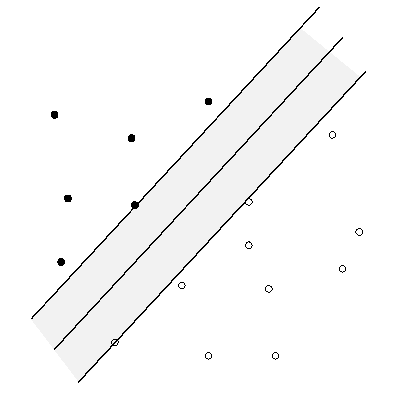
\includegraphics[width=.5\textwidth]{figures/ch08-439.pdf}
\caption*{图8.9 求解稳健线性判别问题(8.23)，得到一个仿射函数，使两组点上的函数值具有最大间隔，其中线性部分受归一化约束。几何上，这是寻找分离两组点的最厚平板。}
\end{figure}
\subsubsection*{支持向量分类器}
两组点无法线性分离时，可以寻找近似分类的仿射函数，例如使误分类点数最小的函数。遗憾的是，这一般是困难的组合优化问题。本节介绍一种基于支持向量分类器的近似线性判别启发式方法。

从可行性问题(8.21)出发，先引入非负变量 $u_1,\ldots,u_N$ 和 $v_1,\ldots,u_M$，放宽约束为
\begin{equation}a^\T x_i-b\geq1-u_i,\quad i=1,\ldots,N,\qquad
 a^\T y_i-b\leq-(1-v_i),\quad i=1,\ldots,M.\tag{8.24}\end{equation}
% Source PDF page 440 (printed p. 426)
\begin{figure}[htbp]\centering
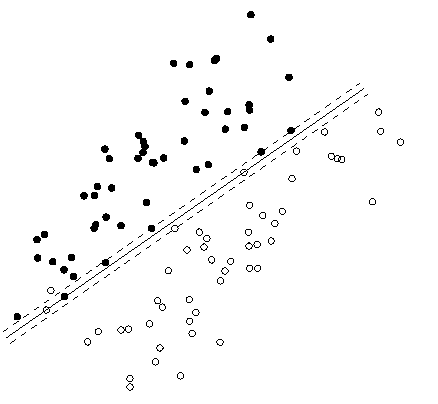
\includegraphics[width=.54\textwidth]{figures/ch08-440.pdf}
\caption*{图8.10 通过线性规划进行近似线性判别。空心圆为 $x_1,\ldots,x_{50}$，实心圆为 $y_1,\ldots,y_{50}$，两组点无法线性分离。实线分类器由 LP(8.25)求得，误分类一个点。虚线为超平面 $a^\T z-b=\pm1$。有四个点分类正确，但位于两条虚线定义的平板内。}
\end{figure}
当 $u=v=0$ 时，恢复原约束；将 $u,v$ 取得充分大，总能使这些不等式可行。可以把 $u_i$ 看作约束 $a^\T x_i-b\geq1$ 的违反程度，$v_i$ 类似。目标是找到 $a,b$ 以及稀疏非负向量 $u,v$，使不等式(8.24)成立。一种启发式做法是最小化各 $u_i,v_i$ 之和，即求解 LP
\begin{equation}\begin{array}{ll}
\text{最小化}&\one^\T u+\one^\T v\\
\text{约束为}&a^\T x_i-b\geq1-u_i,\quad i=1,\ldots,N,\\
&a^\T y_i-b\leq-(1-v_i),\quad i=1,\ldots,M,\\
&u\succeq0,\quad v\succeq0.
\end{array}\tag{8.25}\end{equation}
图8.10给出一个例子，仿射函数 $a^\T z-b$ 将100个点中的一个误分类。不过，当 $0<u_i<1$ 时，点 $x_i$ 被该仿射函数正确分类，却违反不等式 $a^\T x_i-b\geq1$，$y_i$ 的情况类似。LP(8.25)的目标可以解释为以下数量的松弛：违反 $a^\T x_i-b\geq1$ 的 $x_i$ 个数，加上违反 $a^\T y_i-b\leq-1$ 的 $y_i$ 个数。换句话说，它松弛了函数 $a^\T z-b$ 的误分类点数，加上分类正确但位于 $-1<a^\T z-b<1$ 平板内的点数。

更一般地，可以权衡误分类点数与平板 $\{z\mid-1\leq a^\T z-b\leq1\}$ 的宽度，后者为 $2/\norm a_2$。点集 $\{x_1,\ldots,x_N\}$、$\{y_1,\ldots,y_M\}$ 的标准支持向量分类器，
% Source PDF page 441 (printed p. 427)
定义为以下问题的解：
\[\begin{array}{ll}
\text{最小化}&\norm a_2+\gamma(\one^\T u+\one^\T v)\\
\text{约束为}&a^\T x_i-b\geq1-u_i,\quad i=1,\ldots,N,\\
&a^\T y_i-b\leq-(1-v_i),\quad i=1,\ldots,M,\\&u\succeq0,\quad v\succeq0.
\end{array}\]
第一项正比于平板 $-1\leq a^\T z-b\leq1$ 宽度的倒数。第二项与上面的解释相同，是误分类点数的凸松弛，其中也包括平板内的点。正参数 $\gamma$ 给出误分类点数（希望减小）相对于平板宽度（希望增大）的权重。图8.11给出一个例子。
\begin{figure}[htbp]\centering
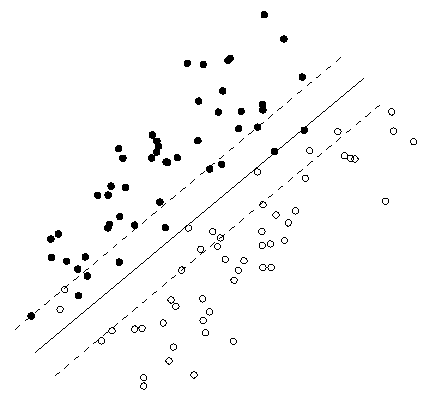
\includegraphics[width=.5\textwidth]{figures/ch08-441.pdf}
\caption*{图8.11 支持向量分类器的近似线性判别，$\gamma=0.1$。实线表示的支持向量分类器误分类三个点。有十五个点分类正确，但落在两条虚线围成的平板 $-1<a^\T z-b<1$ 内。}
\end{figure}
\subsubsection*{通过 logistic 模型进行近似线性判别}
另一种为无法线性分离的两组点寻找近似分类仿射函数的方法，是采用7.1.1节的 logistic 模型。先用 logistic 模型拟合两组点。设随机变量 $z$ 取值零或一，分布通过如下 logistic 模型依赖于确定性解释变量 $u\in\R^n$：
\begin{equation}\begin{aligned}
 \Prob(z=1)&=\frac{\exp(a^\T u-b)}{1+\exp(a^\T u-b)},\\
 \Prob(z=0)&=\frac1{1+\exp(a^\T u-b)}.
\end{aligned}\tag{8.26}\end{equation}
现在假设，给定点集 $\{x_1,\ldots,x_N\}$ 与 $\{y_1,\ldots,y_M\}$ 来自这个 logistic 模型的样本。具体地，$\{x_1,\ldots,x_N\}$ 是 $z=1$ 的 $N$ 个样本所对应的 $u$ 值，$\{y_1,\ldots,y_M\}$ 是 $z=0$ 的 $M$ 个样本所对应的 $u$ 值。
% Source PDF page 442 (printed p. 428)
这允许 $x_i=y_j$，而这种情况会使两组点无法判别。在 logistic 模型中，这只表示两个样本的解释变量相同、结果不同。

从观测样本出发，通过最大似然估计确定 $a,b$，即求解以 $a,b$ 为变量的凸优化问题
\begin{equation}\text{最小化}\quad-l(a,b),\tag{8.27}\end{equation}
其中 $l$ 为对数似然函数，
\[\begin{aligned}
 l(a,b)&=\sum_{i=1}^N(a^\T x_i-b)\\
 &\quad-\sum_{i=1}^N\log(1+\exp(a^\T x_i-b))
       -\sum_{i=1}^M\log(1+\exp(a^\T y_i-b)),
\end{aligned}\]
见7.1.1节。若两组点可线性分离，即存在 $a,b$ 使 $a^\T x_i>b$、$a^\T y_i<b$，则优化问题(8.27)向下无界。

找到 $a,b$ 的最大似然值后，可为两组点建立线性分类器 $f(x)=a^\T x-b$。假设数据点确实由参数为 $a,b$ 的 logistic 模型生成，这个分类器在所有线性分类器中具有最小误分类概率。超平面 $a^\T u=b$ 对应于 $\Prob(z=1)=1/2$ 的点，即两种结果同样可能。图8.12给出一个例子。
\paragraph{注8.1}\textbf{Bayes 解释。}设 $x,z$ 为分别取值于 $\R^n$ 与 $\{0,1\}$ 的随机变量。假设
\[\Prob(z=1)=\Prob(z=0)=1/2,\]
以 $p_0(x),p_1(x)$ 分别表示给定 $z=0$、$z=1$ 时 $x$ 的条件概率密度。假设存在 $a,b$ 使
\[\frac{p_1(x)}{p_0(x)}=e^{a^\T x-b}.\]
许多常见分布满足这一性质。例如，$p_0,p_1$ 可以是 $\R^n$ 上协方差相同、均值不同的两个正态密度，也可以是 $\R_+^n$ 上的两个指数密度。

由 Bayes 公式，
\[\Prob(z=1\mid x=u)=\frac{p_1(u)}{p_1(u)+p_0(u)},\qquad
 \Prob(z=0\mid x=u)=\frac{p_0(u)}{p_1(u)+p_0(u)},\]
从而得到
\[\begin{aligned}
 \Prob(z=1\mid x=u)&=\frac{\exp(a^\T u-b)}{1+\exp(a^\T u-b)},\\
 \Prob(z=0\mid x=u)&=\frac1{1+\exp(a^\T u-b)}.
\end{aligned}\]
% Source PDF page 443 (printed p. 429)
因此，可以把 logistic 模型(8.26)解释为给定 $x=u$ 时 $z$ 的后验分布。
\begin{figure}[htbp]\centering
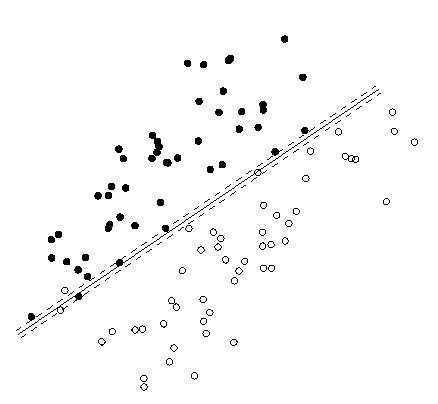
\includegraphics[width=.5\textwidth]{figures/ch08-443.pdf}
\caption*{图8.12 通过 logistic 模型进行近似线性判别。空心圆为 $x_1,\ldots,x_{50}$，实心圆为 $y_1,\ldots,y_{50}$，它们无法线性分离。最大似然 logistic 模型给出深色直线表示的超平面，仅误分类两个点。两条虚线表示 $a^\T u-b=\pm1$，按 logistic 模型，各自对应结果的概率为73\%。有三个点分类正确，但位于两条虚线之间。}
\end{figure}
\subsection{非线性判别}
同样可以在给定函数子空间中寻找非线性函数 $f$，使它在一组点上为正、另一组点上为负：
\[f(x_i)>0,\quad i=1,\ldots,N,\qquad f(y_i)<0,\quad i=1,\ldots,M.\]
只要 $f$ 对定义它的参数是线性或仿射的，这些不等式就能以与线性判别完全相同的方式求解。本节考察几个有趣的特殊情况。
\subsubsection*{二次判别}
设 $f$ 为二次函数：$f(x)=x^\T Px+q^\T x+r$。参数 $P\in\mathbb S^n$、$q\in\R^n$、$r\in\R$ 必须满足
\[x_i^\T Px_i+q^\T x_i+r>0,\quad i=1,\ldots,N,\]
\[y_i^\T Py_i+q^\T y_i+r<0,\quad i=1,\ldots,M,\]
% Source PDF page 444 (printed p. 430)
这是关于变量 $P,q,r$ 的一组严格线性不等式。如同线性判别，$f$ 关于 $P,q,r$ 齐次，因此求解非严格可行性问题
\[x_i^\T Px_i+q^\T x_i+r\geq1,\quad i=1,\ldots,N,\]
\[y_i^\T Py_i+q^\T y_i+r\leq-1,\quad i=1,\ldots,M\]
就能找到严格不等式的解。

分离曲面 $\{z\mid z^\T Pz+q^\T z+r=0\}$ 是二次曲面，两个分类区域
\[\{z\mid z^\T Pz+q^\T z+r\leq0\},\qquad
 \{z\mid z^\T Pz+q^\T z+r\geq0\}\]
由二次不等式定义。因此，求解二次判别问题，等同于判断两组点是否能被二次曲面分离。

通过增加对 $P,q,r$ 的约束，可以规定分离曲面或分类区域的形状。例如，要求 $P\prec0$，意味着分离曲面为椭球面。具体地，就是寻找包含所有 $x_1,\ldots,x_N$，而不含任何 $y_1,\ldots,y_M$ 的椭球。这个二次判别问题可以写成 SDP 可行性问题
\[\begin{array}{ll}
\text{寻找}&P,q,r\\
\text{约束为}&x_i^\T Px_i+q^\T x_i+r\geq1,\quad i=1,\ldots,N,\\
&y_i^\T Py_i+q^\T y_i+r\leq-1,\quad i=1,\ldots,M,\\&P\preceq-I,
\end{array}\]
变量为 $P\in\mathbb S^n$、$q\in\R^n$、$r\in\R$。这里利用关于 $P,q,r$ 的齐次性，将 $P\prec0$ 表示成 $P\preceq-I$。图8.13给出一个例子。
\subsubsection*{多项式判别}
考虑 $\R^n$ 上次数不超过 $d$ 的多项式集合：
\[f(x)=\sum_{i_1+\cdots+i_n\leq d}a_{i_1\cdots i_d}x_1^{i_1}\cdots x_n^{i_n}.\]
求解关于变量 $a_{i_1\cdots i_d}$ 的一组线性不等式，就能确定两组点 $\{x_1,\ldots,x_N\}$、$\{y_1,\ldots,y_M\}$ 能否由这样的多项式分离。几何上，就是检验二者能否由次数不超过 $d$ 的多项式定义的代数曲面分离。

进一步，寻找能分离两组点的最低次数 $\R^n$ 上多项式，可以通过拟凸规划求解，因为多项式次数是系数的拟凸函数。可对 $d$ 二分，每一步求解一个线性规划可行性问题。图8.14给出一个例子。
% Source PDF page 445 (printed p. 431)
\begin{figure}[htbp]\centering
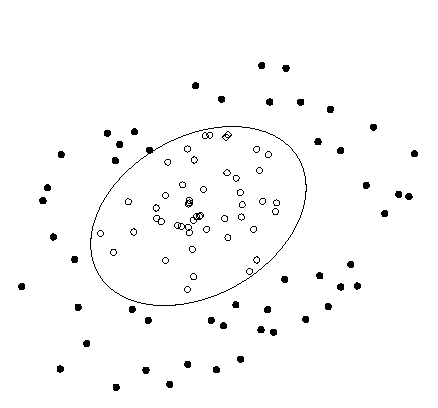
\includegraphics[width=.5\textwidth]{figures/ch08-445a.pdf}
\caption*{图8.13 二次判别，条件为 $P\prec0$。这意味着寻找包含所有 $x_i$（空心圆）且不含任何 $y_i$（实心圆）的椭球。可将其作为 SDP 可行性问题求解。}
\end{figure}
\begin{figure}[htbp]\centering
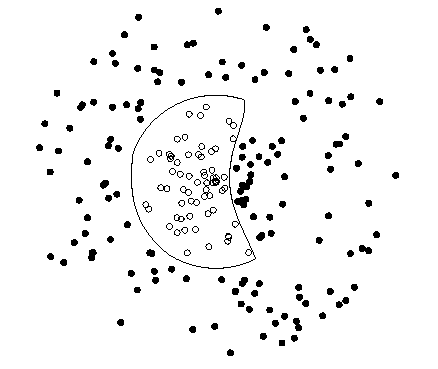
\includegraphics[width=.5\textwidth]{figures/ch08-445b.pdf}
\caption*{图8.14 $\R^2$ 中的最低次数多项式判别。本例中，不存在三次多项式能将 $x_1,\ldots,x_N$（空心圆）与 $y_1,\ldots,y_M$（实心圆）分离，但四次多项式可以，图中画出了它的零水平集。}
\end{figure}
% Source PDF page 446 (printed p. 432)
\section{布置与选址}
本节讨论下列问题的几个变体：在 $\R^2$ 或 $\R^3$ 中有 $N$ 个点，以及必须用链路相连的点对列表。部分点的位置固定；任务是确定其余点的位置，即布置其余点。目标是在满足额外位置约束的条件下，使链路总连接长度的某种度量最小。

例如，可将各点看作公司工厂或仓库的位置，链路看作运输货物的路线，目标是寻找使总运输成本最小的位置。在另一应用中，各点表示集成电路中模块或单元的位置，链路表示连接单元对的导线，目标可以是使连接所有单元的导线总长最小。

用含 $N$ 个节点的无向图描述问题，每个节点代表一个点。与每个节点关联变量 $x_i\in\R^k$，其中 $k=2$ 或 $k=3$，表示其位置。问题是最小化
\[\sum_{(i,j)\in\mathcal A}f_{ij}(x_i,x_j),\]
其中 $\mathcal A$ 是图中全部链路的集合，$f_{ij}:\R^k\times\R^k\to\R$ 为弧 $(i,j)$ 的代价函数。也可以对全部 $i,j$，或对 $i<j$ 求和，在节点 $i,j$ 不相连时令 $f_{ij}=0$。部分坐标向量 $x_i$ 已给定，优化变量为其余坐标。只要各 $f_{ij}$ 凸，这就是凸优化问题。
\subsection{线性设施选址问题}
最简单的版本中，弧 $(i,j)$ 的代价是节点 $i,j$ 之间的距离：$f_{ij}(x_i,x_j)=\norm{x_i-x_j}$，即最小化
\[\sum_{(i,j)\in\mathcal A}\norm{x_i-x_j}.\]
可以采用任意范数，最常见的是欧氏范数与 $\ell_1$ 范数。例如，在电路设计中，单元间的导线通常沿分段线性路径布设，每段为水平或竖直。这称为 Manhattan 布线，因为矩形街区城市中的街道路径也是分段线性的，每条街道沿两条正交轴之一。此时，连接单元 $i,j$ 所需导线长度为 $\norm{x_i-x_j}_1$。

还可以加入非负权重，反映不同弧上单位距离成本的差异：
% Source PDF page 447 (printed p. 433)
\[\sum_{(i,j)\in\mathcal A}w_{ij}\norm{x_i-x_j}.\]
将不相连节点对的权重设为 $w_{ij}=0$，就可更简洁地用目标
\begin{equation}\sum_{i<j}w_{ij}\norm{x_i-x_j}\tag{8.28}\end{equation}
表示这一问题。这个布置问题凸。
\begin{origexample}{8.4}
\textbf{一个自由点。}考虑只有点 $(u,v)\in\R^2$ 自由的情况，最小化它到固定点 $(u_1,v_1),\ldots,(u_K,v_K)$ 的距离之和。
\begin{itemize}
\item \textbf{$\ell_1$ 范数。}可以解析地求出使
\[\sum_{i=1}^K(|u-u_i|+|v-v_i|)\]
最小的点。任意坐标中位点均为最优点，即 $u$ 可取 $\{u_1,\ldots,u_K\}$ 的任意中位数，$v$ 可取 $\{v_1,\ldots,v_K\}$ 的任意中位数。若 $K$ 为奇数，最小点唯一；若 $K$ 为偶数，最优点可能构成一个矩形。
\item \textbf{欧氏范数。}使欧氏距离之和
\[\sum_{i=1}^K\bigl((u-u_i)^2+(v-v_i)^2\bigr)^{1/2}\]
最小的点 $(u,v)$，称为这些固定点的 Weber 点。
\end{itemize}
\end{origexample}
\subsection{布置约束}
下面列举可以加入基本布置问题、并保持凸性的一些约束。可以要求某些位置 $x_i$ 属于指定凸集，例如某条直线、区间、正方形或椭球；可以限制一个点相对于其他一个或多个点的位置，例如限制一对点之间的距离；也可以规定相对位置，例如某点必须位于另一点左侧。

一组点的包围盒是包含这些点的最小矩形。例如，通过加入约束
\[u\preceq x_i\preceq v,\quad i=1,\ldots,p,\qquad2\one^\T(v-u)\leq P_{\max},\]
可以要求点 $x_1,\ldots,x_p$ 位于周长不超过 $P_{\max}$ 的包围盒内，其中 $u,v$ 为附加变量。
% Source PDF page 448 (printed p. 434)
\subsection{非线性设施选址问题}
更一般地，可以给每条弧指定一个关于长度非线性递增的代价，即
\[\text{最小化}\quad\sum_{i<j}w_{ij}h(\norm{x_i-x_j}),\]
其中 $h$ 在 $\R_+$ 上递增且凸，$w_{ij}\geq0$。称为非线性布置或非线性设施选址问题。

一种常见情况采用欧氏范数与 $h(z)=z^2$，即最小化
\[\sum_{i<j}w_{ij}\norm{x_i-x_j}_2^2.\]
它称为二次布置问题。若仅有线性等式约束，可解析求解；若约束为线性等式与不等式，则可作为 QP 求解。
\begin{origexample}{8.5}
\textbf{一个自由点。}考虑仅有一个点 $x$ 自由，最小化到固定点 $x_1,\ldots,x_K$ 的欧氏距离平方之和：
\[\norm{x-x_1}_2^2+\norm{x-x_2}_2^2+\cdots+\norm{x-x_K}_2^2.\]
求导可知，最优 $x$ 为
\[\frac1K(x_1+x_2+\cdots+x_K),\]
即固定点的平均值。
\end{origexample}
其他一些有意义的选择包括死区宽度为 $2\gamma$ 的死区函数 $h$，定义为
\[h(z)=\begin{cases}0,&|z|\leq\gamma,\\|z-\gamma|,&|z|\geq\gamma,\end{cases}\]
以及二次—线性函数 $h$，定义为
\[h(z)=\begin{cases}z^2,&|z|\leq\gamma,\\2\gamma|z|-\gamma^2,&|z|\geq\gamma.\end{cases}\]
\begin{origexample}{8.6}
考虑 $\R^2$ 中具有6个自由点、8个固定点和27条链路的布置问题。图8.15—8.17展示分别采用准则
\[\sum_{(i,j)\in\mathcal A}\norm{x_i-x_j}_2,\qquad
 \sum_{(i,j)\in\mathcal A}\norm{x_i-x_j}_2^2,\qquad
 \sum_{(i,j)\in\mathcal A}\norm{x_i-x_j}_2^4\]
的最优解，即分别使用惩罚函数 $h(z)=z$、$h(z)=z^2$、$h(z)=z^4$。图中还给出了相应链路长度的分布。

比较结果可见，线性布置将自由点集中在小区域内，二次和四次布置则将点分散在更大区域。线性布置包含许多很短的链路和少数很长的链路：3条短于0.2，2条长于1.5。二次惩罚相对于短链路，更重地惩罚长链路；对于短于0.1的链路，惩罚几乎可忽略。
% Source PDF page 449 (printed p. 435)
\begin{figure}[htbp]\centering
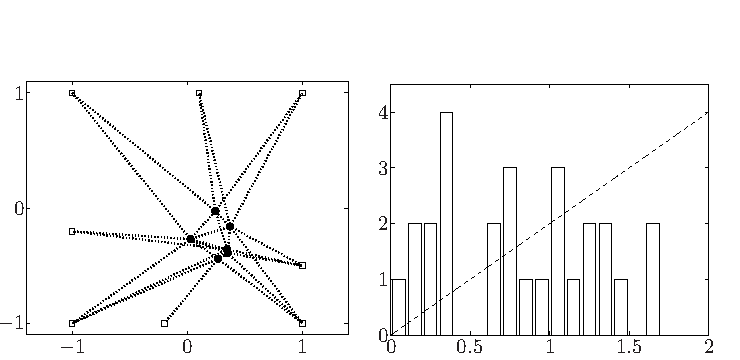
\includegraphics[width=.85\textwidth]{figures/ch08-449a.pdf}
\caption*{图8.15 线性布置。问题包含6个自由点（圆点）、8个固定点（方块）和27条链路。自由点坐标使链路欧氏长度之和最小。右图给出27条链路长度的分布。虚线是缩放后的惩罚函数 $h(z)=z$。}
\end{figure}
\begin{figure}[htbp]\centering
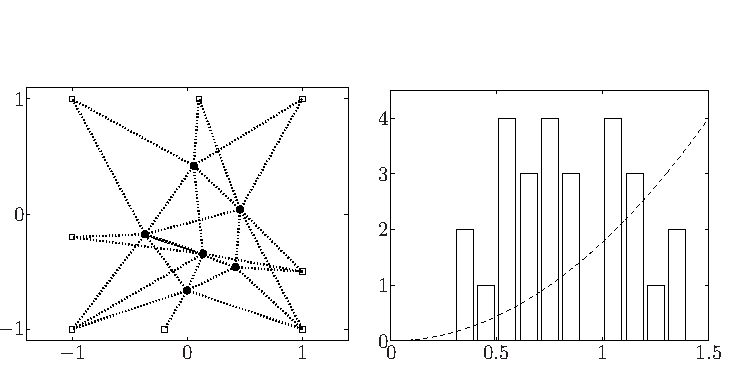
\includegraphics[width=.85\textwidth]{figures/ch08-449b.pdf}
\caption*{图8.16 二次布置。与图8.15采用相同数据，使链路欧氏长度平方和最小。虚线是缩放后的惩罚函数 $h(z)=z^2$。}
\end{figure}
% Source PDF page 450 (printed p. 436)
\begin{figure}[htbp]\centering
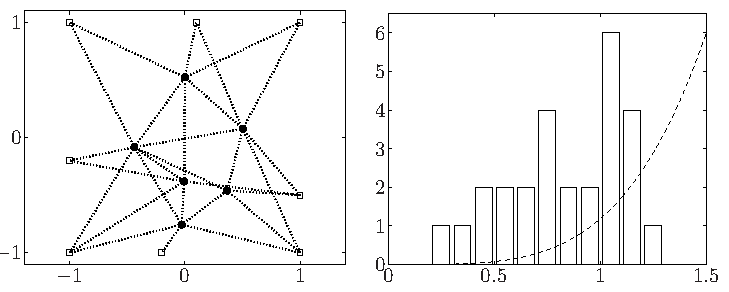
\includegraphics[width=.85\textwidth]{figures/ch08-450.pdf}
\caption*{图8.17 四次布置。使链路欧氏长度的四次方之和最小。虚线是缩放后的惩罚函数 $h(z)=z^4$。}
\end{figure}
因此，二次布置的最大长度更短，小于1.4，但短链路也更少。四次函数对长链路的惩罚更重，在更宽的区间（零至约0.4）内几乎可忽略。因此，最大长度比二次布置更短，但接近最大长度的链路也更多。
\end{origexample}
\subsection{带路径约束的选址问题}
\subsubsection*{路径约束}
沿点 $x_1,\ldots,x_N$ 的一条含 $p$ 条链路的路径，由节点序列 $i_0,\ldots,i_p\in\{1,\ldots,N\}$ 描述。路径长度为
\[\norm{x_{i_1}-x_{i_0}}+\norm{x_{i_2}-x_{i_1}}+\cdots+\norm{x_{i_p}-x_{i_{p-1}}},\]
这是 $x_1,\ldots,x_N$ 的凸函数，因此对路径长度规定上界是凸约束。有些有意义的布置问题包含路径约束，或目标基于路径长度。下面介绍一个典型例子，目标是一组路径中的最大路径长度。
\subsubsection*{极小极大延迟布置}
考虑节点为 $1,\ldots,N$ 的有向无环图，弧或链路由有序对集合 $\mathcal A$ 表示：$(i,j)\in\mathcal A$ 当且仅当有一条弧从 $i$ 指向 $j$。若没有 $\mathcal A$ 中的弧指向节点 $i$，称其为源节点；若没有弧从它离开，称其为汇节点或目的节点。关心图中从源节点开始、在汇节点结束的极大路径。

图中的弧用于表示某种流，例如货物或信息，在节点位置为 $x_1,\ldots,x_N$ 的网络中流动。流从一个源节点开始，
% Source PDF page 451 (printed p. 437)
沿路径逐个节点移动，最后到达汇节点或目的节点。用相邻节点间距离描述货物的传播时间或运输时间；一条路径的总延迟或传播时间，正比于相邻节点距离之和。

现在可以描述极小极大延迟布置问题：部分节点位置固定，其余位置自由，即为优化变量；目标是选择自由节点位置，使任意源节点至汇节点路径的最大总延迟最小。这显然是凸问题，因为目标
\begin{equation}\begin{split}
T_{\max}=\max\{&\norm{x_{i_1}-x_{i_0}}+\cdots+\norm{x_{i_p}-x_{i_{p-1}}}\mid\\
 &i_0,\ldots,i_p\text{ 为源节点至汇节点的路径}\}
\end{split}\tag{8.29}\end{equation}
是位置 $x_1,\ldots,x_N$ 的凸函数。

虽然最小化式(8.29)是凸问题，源至汇路径的数量却可能很大，随节点数或弧数指数增长。有一种有用的重新表述，可以避免枚举所有源至汇路径。

先说明如何计算最大延迟 $T_{\max}$，其效率远高于逐条计算源至汇路径的延迟再取最大值。令 $\tau_k$ 为从节点 $k$ 到某个汇节点的全部路径中最大总延迟。若 $k$ 为汇节点，显然 $\tau_k=0$。考虑节点 $k$，它的出弧通向节点 $j_1,\ldots,j_p$。从 $k$ 出发、到汇节点结束的路径，第一条弧必通向这些节点之一。若路径先到 $j_i$，再沿从那里到汇节点的最长路径，总长度为
\[\norm{x_{j_i}-x_k}+\tau_{j_i},\]
即通向 $j_i$ 的弧长，加上 $j_i$ 到汇节点的最长路径总长。因此，从 $k$ 到汇节点的路径最大延迟满足
\begin{equation}
 \tau_k=\max\{\norm{x_{j_1}-x_k}+\tau_{j_1},\ldots,\norm{x_{j_p}-x_k}+\tau_{j_p}\}.\tag{8.30}
\end{equation}
这是一个简单的动态规划论证。

等式(8.30)给出计算任意节点最大延迟的递推：从最大延迟为零的汇节点出发，利用式(8.30)反向推进，直到全部源节点。这类路径的最大延迟就是所有 $\tau_k$ 的最大值，并将在某个源节点取得。这一动态规划递推表明，无须枚举全部路径，就能递归计算任意源至汇路径上的最大延迟。所需算术运算次数约等于链路数。

下面利用基于式(8.30)的递推，建立极小极大延迟布置问题。可将问题写为
\[\begin{array}{ll}
\text{最小化}&\max\{\tau_k\mid k\text{ 为源节点}\}\\
\text{约束为}&\tau_k=0,\quad k\text{ 为汇节点},\\
&\tau_k=\max\{\norm{x_j-x_k}+\tau_j\mid\text{存在从 }k\text{ 到 }j\text{ 的弧}\},
\end{array}\]
% Source PDF page 452 (printed p. 438)
变量为 $\tau_1,\ldots,\tau_N$ 及自由位置。这个问题不凸，但将等式替换为不等式后，可得到等价的凸形式。引入新变量 $T_1,\ldots,T_N$，分别作为 $\tau_1,\ldots,\tau_N$ 的上界。所有汇节点取 $T_k=0$，用不等式
\[T_k\geq\max\{\norm{x_{j_1}-x_k}+T_{j_1},\ldots,\norm{x_{j_p}-x_k}+T_{j_p}\}\]
代替式(8.30)。若这些不等式成立，则 $T_k\geq\tau_k$。建立问题
\[\begin{array}{ll}
\text{最小化}&\max\{T_k\mid k\text{ 为源节点}\}\\
\text{约束为}&T_k=0,\quad k\text{ 为汇节点},\\
&T_k\geq\max\{\norm{x_j-x_k}+T_j\mid\text{存在从 }k\text{ 到 }j\text{ 的弧}\}.
\end{array}\]
它以 $T_1,\ldots,T_N$ 及自由位置为变量，是凸问题，并求解了极小极大延迟选址问题。
\section{平面布局}
在布置问题中，变量表示需要最优放置的若干点的坐标。平面布局问题可以看作从两个方面推广布置问题：
\begin{itemize}
\item 待放置对象是与坐标轴对齐的矩形或盒，而不是点，且不能重叠；
\item 每个矩形或盒可以在一定范围内重新配置。例如，固定各矩形的面积，但不分别固定长度与高度。
\end{itemize}
目标通常是最小化包围盒的大小，例如面积、体积或周长；包围盒是包含全部待配置、待放置盒子的最小盒。

不重叠约束使一般平面布局成为复杂的组合优化或矩形装填问题。不过，若已指定盒子的相对位置，有几类布局问题可以建立为凸优化。本节研究其中一些，主要考虑二维情况，对高维推广中不明显之处作简要说明。

有 $N$ 个单元或模块 $C_1,\ldots,C_N$，需要配置并放入宽 $W$、高 $H$、左下角在 $(0,0)$ 的矩形内。第 $i$ 个单元的几何形状和位置，由宽 $w_i$、高 $h_i$ 以及左下角坐标 $(x_i,y_i)$ 指定，见图8.18。

问题变量为 $x_i,y_i,w_i,h_i$，$i=1,\ldots,N$，以及外包矩形的宽 $W$ 和高 $H$。所有布局问题都要求各单元位于外包矩形内，即
\begin{equation}
 x_i\geq0,\quad y_i\geq0,\quad x_i+w_i\leq W,\quad y_i+h_i\leq H,\quad i=1,\ldots,N.\tag{8.31}
\end{equation}
% Source PDF page 453 (printed p. 439)
\begin{figure}[htbp]\centering
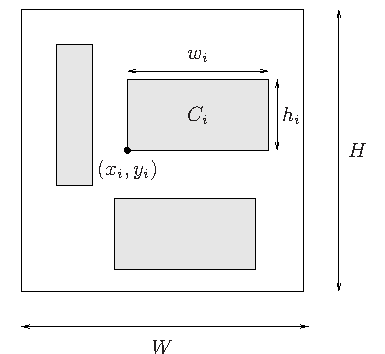
\includegraphics[width=.5\textwidth]{figures/ch08-453.pdf}
\caption*{图8.18 平面布局问题。将不重叠的矩形单元放入宽 $W$、高 $H$、左下角为 $(0,0)$ 的矩形内。第 $i$ 个单元由宽 $w_i$、高 $h_i$ 及左下角坐标 $(x_i,y_i)$ 指定。}
\end{figure}
还要求各单元除边界外不重叠：
\[\operatorname{int}(C_i\cap C_j)=\varnothing,\qquad i\ne j.\]
也可以要求单元之间有正的最小间隙。不重叠约束成立，当且仅当对 $i\ne j$，以下条件至少一个成立：$C_i$ 位于 $C_j$ 左侧、右侧、下方或上方。

这四个几何条件对应于不等式
\begin{equation}
 x_i+w_i\leq x_j,\quad\text{或 }x_j+w_j\leq x_i,\quad
 \text{或 }y_i+h_i\leq y_j,\quad\text{或 }y_j+h_j\leq y_i,\tag{8.32}
\end{equation}
对每个 $i\ne j$ 至少一条成立。这些约束具有组合性质：每一对不同单元，四个不等式中至少一个必须成立。
\subsection{相对位置约束}
相对位置约束的思路是，为每一对单元指定四种可能位置关系中的一种，即左、右、上、下。一个简单方法是在 $\{1,\ldots,N\}$ 上给出两个关系：$\mathcal L$ 表示“位于左侧”，$\mathcal B$ 表示“位于下方”。规定 $(i,j)\in\mathcal L$ 时，$C_i$ 位于 $C_j$ 左侧；$(i,j)\in\mathcal B$ 时，$C_i$ 位于 $C_j$ 下方。于是得到约束
\begin{equation}
 x_i+w_i\leq x_j\text{ 对 }(i,j)\in\mathcal L,\qquad
 y_i+h_i\leq y_j\text{ 对 }(i,j)\in\mathcal B,\tag{8.33}
\end{equation}
% Source PDF page 454 (printed p. 440)
其中 $i,j=1,\ldots,N$。为确保 $\mathcal L,\mathcal B$ 指定每对单元的相对位置，要求对每个 $i\ne j$，以下之一成立：
\[(i,j)\in\mathcal L,\qquad(j,i)\in\mathcal L,\qquad
 (i,j)\in\mathcal B,\qquad(j,i)\in\mathcal B,\]
并要求 $(i,i)\notin\mathcal L$、$(i,i)\notin\mathcal B$。不等式(8.33)是关于变量的 $N(N-1)/2$ 条线性不等式。它们蕴含不重叠不等式(8.32)，后者由 $N(N-1)/2$ 个“四条线性不等式的析取”组成。

可以假设 $\mathcal L,\mathcal B$ 反对称，即 $(i,j)\in\mathcal L\Rightarrow(j,i)\notin\mathcal L$，并且传递，即 $(i,j)\in\mathcal L$、$(j,k)\in\mathcal L\Rightarrow(i,k)\in\mathcal L$。否则相对位置约束显然不可行。传递性对应于一个直接的条件：若 $C_i$ 在 $C_j$ 左侧，而 $C_j$ 在 $C_k$ 左侧，则 $C_i$ 必在 $C_k$ 左侧。此时 $(i,k)\in\mathcal L$ 对应的不等式冗余，由另外两条蕴含。利用关系 $\mathcal L,\mathcal B$ 的传递性，可以删除冗余约束，得到紧凑的相对位置不等式组。

最小的相对位置约束集，可以方便地用两个有向无环图 $\mathcal H,\mathcal V$ 描述，分别表示水平与竖直。两个图都含 $N$ 个节点，对应布局中的 $N$ 个单元。图 $\mathcal H$ 生成关系 $\mathcal L$：$(i,j)\in\mathcal L$ 当且仅当 $\mathcal H$ 中存在从 $i$ 到 $j$ 的有向路径。类似地，$\mathcal V$ 生成 $\mathcal B$：$(i,j)\in\mathcal B$ 当且仅当 $\mathcal V$ 中存在从 $i$ 到 $j$ 的有向路径。为确保每对单元都有相对位置约束，要求在两个图之一中，存在从这对单元之一通向另一单元的有向路径。

显然，只需施加两个图中边所对应的不等式，其余都由传递性推出。于是得到
\begin{equation}
 x_i+w_i\leq x_j\text{ 对 }(i,j)\in\mathcal H,\qquad
 y_i+h_i\leq y_j\text{ 对 }(i,j)\in\mathcal V,\tag{8.34}
\end{equation}
每条边对应一条线性不等式。式(8.34)是式(8.33)的子集，并与之等价。

同样，$4N$ 条不等式(8.31)可以缩减为最小等价组。约束 $x_i\geq0$ 只需对最左侧单元施加，即在关系 $\mathcal L$ 中极小的 $i$；它们对应 $\mathcal H$ 中无入边的源节点。类似地，$x_i+w_i\leq W$ 只需对最右侧单元施加。竖直方向的外包盒不等式也可以同样精简。得到最小等价外包盒约束：
\begin{equation}\begin{aligned}
 x_i&\geq0\text{ 对 }\mathcal L\text{ 中极小的 }i,&x_i+w_i&\leq W\text{ 对 }\mathcal L\text{ 中极大的 }i,\\
 y_i&\geq0\text{ 对 }\mathcal B\text{ 中极小的 }i,&y_i+h_i&\leq H\text{ 对 }\mathcal B\text{ 中极大的 }i.
\end{aligned}\tag{8.35}\end{equation}
图8.19给出一个简单例子。其中，$\mathcal L$ 中极小、即最左侧的单元为 $C_1,C_2,C_4$，唯一最右侧单元为 $C_5$。规定水平相对位置的最小不等式组为
\[x_1\geq0,\quad x_2\geq0,\quad x_4\geq0,\quad x_5+w_5\leq W,\quad x_1+w_1\leq x_3,\]
\[x_2+w_2\leq x_3,\qquad x_3+w_3\leq x_5,\qquad x_4+w_4\leq x_5.\]
% Source PDF page 455 (printed p. 441)
\begin{figure}[htbp]\centering
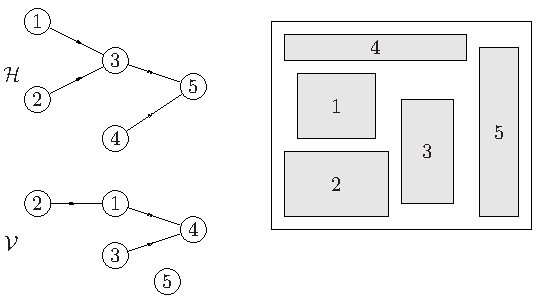
\includegraphics[width=.7\textwidth]{figures/ch08-455.pdf}
\caption*{图8.19 用水平图 $\mathcal H$、竖直图 $\mathcal V$ 规定单元相对位置的例子。若 $\mathcal H$ 中存在从 $i$ 到 $j$ 的路径，单元 $i$ 必须位于单元 $j$ 左侧；若 $\mathcal V$ 中存在从 $i$ 到 $j$ 的路径，单元 $i$ 必须位于单元 $j$ 下方。右侧布局满足两图规定的相对位置。}
\end{figure}
规定竖直相对位置的最小不等式组为
\[y_2\geq0,\quad y_3\geq0,\quad y_5\geq0,\quad y_4+h_4\leq H,\quad y_5+h_5\leq H,\]
\[y_2+h_2\leq y_1,\qquad y_1+h_1\leq y_4,\qquad y_3+h_3\leq y_4.\]
\subsection{通过凸优化进行平面布局}
本模型的变量为外包盒宽、高 $W,H$，以及单元的宽、高和位置 $w_i,h_i,x_i,w_i$，$i=1,\ldots,N$。施加外包盒约束(8.35)和相对位置约束(8.34)，它们都是线性不等式。目标取外包盒周长 $2(W+H)$，是变量的线性函数。下面列出一些能够表示成关于变量的凸不等式或线性等式的约束。
\subsubsection*{最小间距}
将相对位置约束 $x_i+w_i\leq x_j$，$(i,j)\in\mathcal H$，改为 $x_i+w_i+\rho\leq x_j$，并对竖直图作同样处理，就能规定单元间的最小间距 $\rho>0$。可以给两个图中每条边指定不同的最小间距。另一种选择是固定 $W,H$，以最大化最小间距 $\rho$ 为目标。
% Source PDF page 456 (printed p. 442)
\subsubsection*{单元最小面积}
为每个单元指定最小面积，即要求 $w_ih_i\geq A_i$，$A_i>0$。这些约束有多种凸不等式表示，例如 $w_i\geq A_i/h_i$、$(w_ih_i)^{1/2}\geq A_i^{1/2}$，或 $\log w_i+\log h_i\geq\log A_i$。
\subsubsection*{长宽比约束}
可以规定每个单元长宽比的上下界：
\[l_i\leq h_i/w_i\leq u_i.\]
两边乘以 $w_i$，即可化为线性不等式。也可以固定单元长宽比，此时得到线性等式约束。
\subsubsection*{对齐约束}
可以要求两个单元的某条边或中心线对齐。例如，单元 $i$ 的水平中心线与单元 $j$ 顶边对齐时，
\[y_i+h_i/2=y_j+h_j.\]
这些是线性等式约束。也可以同样要求单元紧贴外包盒边界。
\subsubsection*{对称约束}
可以要求成对单元关于某条竖直轴或水平轴对称，轴可以固定或浮动，即位置给定或未给定。例如，要求单元 $i,j$ 关于竖直轴 $x=x_{\mathrm{axis}}$ 对称，可施加线性等式
\[x_{\mathrm{axis}}-(x_i+w_i/2)=x_j+w_j/2-x_{\mathrm{axis}}.\]
加入这些等式，并将 $x_{\mathrm{axis}}$ 作为新变量，就能要求多对单元关于某条未指定的竖直轴对称。
\subsubsection*{相似约束}
用等式 $w_i=aw_j$、$h_i=ah_j$，可要求单元 $i$ 是单元 $j$ 缩放 $a$ 倍再平移后的结果。这里缩放因子 $a$ 必须固定。只施加其中一条约束，就要求一个单元的宽或高为另一个的给定倍数。
\subsubsection*{包含约束}
可以要求某个单元包含给定点，这施加两条线性不等式；也可以要求单元位于给定多面体内，同样通过线性不等式实现。
% Source PDF page 457 (printed p. 443)
\subsubsection*{距离约束}
可以施加各种约束，限制单元对之间的距离。最简单的是限制单元 $i,j$ 中心点之间的距离，也可以是单元上的其他固定点，例如左下角。限制两中心的距离，可用凸不等式
\[\norm{(x_i+w_i/2,y_i+h_i/2)-(x_j+w_j/2,y_j+h_j/2)}\leq D_{ij}.\]
如同布置问题，也可以限制距离之和，或以距离之和作为目标。

还可以限制单元 $i,j$ 之间的距离 $\dist(C_i,C_j)$，即各单元中一点之间的最小距离。一般可如下处理。为限制范数 $\norm{\cdot}$ 下的距离，引入四个新变量 $u_i,v_i,u_j,v_j$。坐标对 $(u_i,v_i)$ 表示 $C_i$ 中一点，$(u_j,v_j)$ 表示 $C_j$ 中一点，为此施加线性不等式
\[x_i\leq u_i\leq x_i+w_i,\qquad y_i\leq v_i\leq y_i+h_i,\]
并对单元 $j$ 作同样处理。最后，加入凸不等式
\[\norm{(u_i,v_i)-(u_j,v_j)}\leq D_{ij}\]
限制 $\dist(C_i,C_j)$。

在许多特殊情况下，可以利用相对位置约束，或导出更显式的模型，更高效地表示距离约束。例如，考虑 $\ell_\infty$ 范数，并假设相对位置约束规定单元 $i$ 在单元 $j$ 左侧。两单元的水平间距为 $x_j-(x_i+w_i)$。此时 $\dist(C_i,C_j)\leq D_{ij}$ 当且仅当
\[x_j-(x_i+w_i)\leq D_{ij},\quad y_j-(y_i+h_i)\leq D_{ij},\quad
 y_i-(y_j+h_j)\leq D_{ij}.\]
第一个不等式说明，单元 $i$ 右边与单元 $j$ 左边的水平间距不超过 $D_{ij}$；第二个说明，单元 $j$ 底边高出单元 $i$ 顶边不超过 $D_{ij}$；第三个说明，单元 $i$ 底边高出单元 $j$ 顶边不超过 $D_{ij}$。三者合起来等价于 $\dist(C_i,C_j)\leq D_{ij}$，无须引入新变量。

可以同样限制两个单元的 $\ell_1$ 或 $\ell_2$ 距离。引入新变量 $d_v$，作为单元间竖直间距的上界。限制 $\ell_1$ 距离时加入
\[y_j-(y_i+h_i)\leq d_v,\qquad y_i-(y_j+h_j)\leq d_v,\qquad d_v\geq0,\]
以及
\[x_j-(x_i+w_i)+d_v\leq D_{ij}.\]
第一项是水平间距，第二项是竖直间距上界。限制欧氏距离时，将最后一条替换为
\[(x_j-(x_i+w_i))^2+d_v^2\leq D_{ij}^2.\]
% Source PDF page 458 (printed p. 444)
\begin{figure}[htbp]\centering
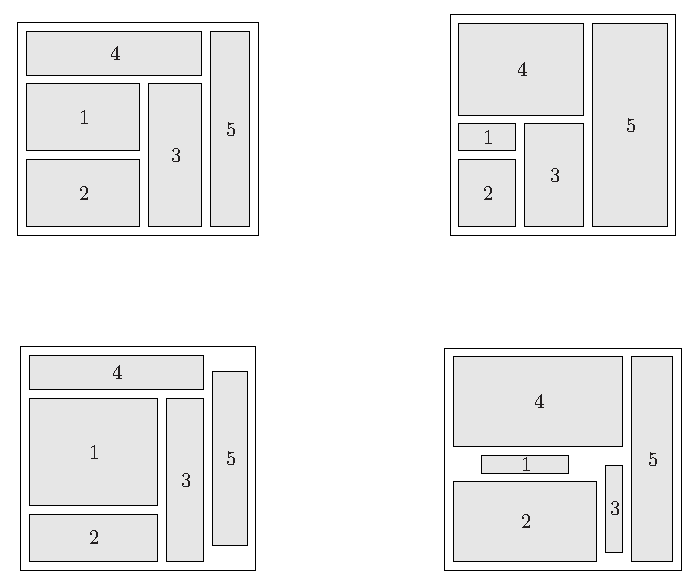
\includegraphics[width=.8\textwidth]{figures/ch08-458.pdf}
\caption*{图8.20 四个最优平面布局实例，采用图8.19的相对位置约束。每个实例都以周长最小为目标，单元之间采用相同最小间距约束，并要求长宽比在 $1/5$ 与5之间。四个实例的差别在于各单元的最小面积要求，但最小面积之和相同。}
\end{figure}
\begin{origexample}{8.7}
图8.20给出5个单元的例子，采用图8.19的顺序约束，以及四组不同约束。每例都施加相同的最小间距要求及相同长宽比约束 $1/5\leq w_i/h_i\leq5$。四例的差别在于各单元最小面积 $A_i$ 不同。选择 $A_i$ 时，使每例总最小面积要求 $\sum_{i=1}^5A_i$ 相同。
\end{origexample}
\subsection{通过几何规划进行平面布局}
平面布局问题也可以写成关于变量 $x_i,y_i,w_i,h_i,W,H$ 的几何规划。这种模型可处理的目标与约束，与凸模型略有不同。

首先，外包盒约束(8.35)与相对位置约束(8.34)都是正项式不等式，因为左端是变量之和，右端是单个变量，因而为单项式。
% Source PDF page 459 (printed p. 445)
将这些不等式除以右端，就得到标准正项式不等式。

在几何规划模型中，可以最小化外包盒面积，因为 $WH$ 为单项式，因而也是正项式。也可以精确指定每个单元面积，因为 $w_ih_i=A_i$ 是单项式等式约束。另一方面，几何规划模型不能处理对齐、对称和距离约束；但可以处理相似约束，而且可以要求单元相似而不指定缩放比例，将其作为另一个变量即可。
% Source PDF page 460 (printed p. 446)
\section*{文献说明}
\addcontentsline{toc}{section}{文献说明}
8.3.3节的欧氏距离矩阵刻画见 Schoenberg [Sch35]，也见 Gower [Gow85]。

本书沿用 Grötschel、Lovász 和 Schrijver [GLS88，第69页] 的 Löwner--John 椭球称谓。8.4节椭球近似的效率结论由 John [Joh85] 证明。Boyd、El Ghaoui、Feron 和 Balakrishnan [BEFB94，第3.7节] 针对由椭球的并、交或和定义的集合，给出几种椭球近似问题的凸模型。

8.5节的不同中心用于设计中心化，例如 Seifi、Ponnambalan 和 Vlach [SPV99]，以及割平面方法，参见 Elzinga 和 Moore [EM75]、Tarasov、Khachiyan 和 Èrlikh [TKE88]、Ye [Ye97，第8章]。由对数障碍 Hessian 定义的内椭球（原书第420页）有时称为 Dikin 椭球，是 Dikin 线性规划与二次规划算法的基础 [Dik67]。解析中心处外椭球的表达式由 Sonnevend [Son86] 给出。向非多面体凸集的推广，见 Boyd 和 El Ghaoui [BE93]、Jarre [Jar94]，以及 Nesterov 和 Nemirovski [NN94，第34页]。

自20世纪60年代起，凸优化就用于线性与非线性判别，见 Mangasarian [Man65] 和 Rosen [Ros65]。模式分类的标准教材包括 Duda、Hart 和 Stork [DHS99]，以及 Hastie、Tibshirani 和 Friedman [HTF01]。支持向量分类器的详细讨论，见 Vapnik [Vap00] 或 Schölkopf 和 Smola [SS01]。

例8.4的 Weber 点以 Weber [Web71] 命名。线性与二次布置用于电路设计，见 Kleinhaus、Sigl、Johannes 和 Antreich [KSJA91, SDJ91]。Sherwani [She99] 是近年来对 VLSI 电路设计中的布置、布局、平面规划及其他几何优化算法的综述。
% Source PDF page 461 (printed p. 447)
\section*{习题}
\addcontentsline{toc}{section}{习题}
\subsection*{在集合上的投影}
\paragraph{8.1}\textit{投影的唯一性。}证明，若 $C\subseteq\R^n$ 非空、闭且凸，范数 $\norm{\cdot}$ 严格凸，则对每个 $x_0$，都恰好存在一个离它最近的 $x\in C$。换句话说，$x_0$ 在 $C$ 上的投影唯一。
\paragraph{8.2}[Web94, Val64] \textit{凸性的 Chebyshev 刻画。}若对每个 $x_0\in\R^n$，集合 $C\in\R^n$ 中都存在唯一离 $x_0$ 最近的点，距离采用欧氏范数，则称 $C$ 为 Chebyshev 集。根据习题8.1，每个非空闭凸集都是 Chebyshev 集。本题证明逆命题，即 Motzkin 定理。

设 $C\in\R^n$ 为 Chebyshev 集。
\begin{enumerate}[label=(\alph*)]
\item 证明 $C$ 非空且闭。
\item 证明在 $C$ 上的欧氏投影 $P_C$ 连续。
\item 设 $x_0\notin C$。证明，对所有 $x=\theta x_0+(1-\theta)P_C(x_0)$、$0\leq\theta\leq1$，有 $P_C(x)=P_C(x_0)$。
\item 设 $x_0\notin C$。证明，对所有 $x=\theta x_0+(1-\theta)P_C(x_0)$、$\theta\geq1$，有 $P_C(x)=P_C(x_0)$。
\item 合并(c)与(d)，可知以 $P_C(x_0)$ 为起点、方向为 $x_0-P_C(x_0)$ 的射线上，所有点的投影都是 $P_C(x_0)$。证明这意味着 $C$ 凸。
\end{enumerate}
\paragraph{8.3}\textit{在正常锥上的欧氏投影。}
\begin{enumerate}[label=(\alph*)]
\item \textit{非负正交象限。}证明在非负正交象限上的欧氏投影由原书第399页的表达式给出。
\item \textit{半正定锥。}证明在半正定锥上的欧氏投影由原书第399页的表达式给出。
\item \textit{二阶锥。}证明 $(x_0,t_0)$ 在二阶锥
\[K=\{(x,t)\in\R^{n+1}\mid\norm x_2\leq t\}\]
上的欧氏投影为
\[P_K(x_0,t_0)=\begin{cases}
0,&\norm{x_0}_2\leq-t_0,\\
(x_0,t_0),&\norm{x_0}_2\leq t_0,\\
\tfrac12(1+t_0/\norm{x_0}_2)(x_0,\norm{x_0}_2),&\norm{x_0}_2\geq|t_0|.
\end{cases}\]
\end{enumerate}
\paragraph{8.4}点在凸集上的欧氏投影，给出一个简单的分离超平面：
\[(P_C(x_0)-x_0)^\T\bigl(x-\tfrac12(x_0+P_C(x_0))\bigr)=0.\]
找出反例，说明这个构造对一般范数不成立。
\paragraph{8.5}[HUL93，第1卷，第154页] \textit{深度函数与到边界的有符号距离。}设 $C\subseteq\R^n$ 为非空凸集，$\dist(x,C)$ 为点 $x$ 在某范数下到 $C$ 的距离。已知 $\dist(x,C)$ 关于 $x$ 凸。
\begin{enumerate}[label=(\alph*)]
\item 证明深度函数
\[\operatorname{depth}(x,C)=\dist(x,\R^n\setminus C)\]
在 $x\in C$ 时凹。
\item 到 $C$ 边界的有符号距离定义为
\[s(x)=\begin{cases}\dist(x,C),&x\notin C,\\-\operatorname{depth}(x,C),&x\in C.\end{cases}\]
因此，$s(x)$ 在 $C$ 外为正，边界上为零，内部为负。证明 $s$ 为凸函数。
\end{enumerate}
% Source PDF page 462 (printed p. 448)
\subsection*{集合之间的距离}
\paragraph{8.6}设 $C,D$ 为凸集。
\begin{enumerate}[label=(\alph*)]
\item 证明 $\dist(C,x+D)$ 关于 $x$ 凸。
\item 证明 $\dist(tC,x+tD)$ 在 $t>0$ 时关于 $(x,t)$ 凸。
\end{enumerate}
\paragraph{8.7}\textit{椭球的分离。}设两个椭球定义为
\[\mathcal E_1=\{x\mid(x-x_1)^\T P_1^{-1}(x-x_1)\leq1\},\qquad
 \mathcal E_2=\{x\mid(x-x_2)^\T P_2^{-1}(x-x_2)\leq1\},\]
其中 $P_1,P_2\in\mathbb S_{++}^n$。证明，$\mathcal E_1\cap\mathcal E_2=\varnothing$ 当且仅当存在 $a\in\R^n$ 使
\[\norm{P_1^{1/2}a}_2+\norm{P_2^{1/2}a}_2<a^\T(x_1-x_2).\]
\paragraph{8.8}\textit{多面体的相交与包含。}设两个多面体定义为
\[P_1=\{x\mid Ax\preceq b\},\qquad P_2=\{x\mid Fx\preceq g\},\]
其中 $A\in\R^{m\times n}$、$b\in\R^m$、$F\in\R^{p\times n}$、$g\in\R^p$。说明如何通过求解一个或数量不多的 LP 可行性问题完成以下任务。
\begin{enumerate}[label=(\alph*)]
\item 找到交集 $P_1\cap P_2$ 中的一点。
\item 判断是否 $P_1\subseteq P_2$。
\end{enumerate}
对以下方式定义的两个多面体重复上述问题：
\[P_1=\conv\{v_1,\ldots,v_K\},\qquad P_2=\conv\{w_1,\ldots,w_L\},\]
其中 $v_1,\ldots,v_K,w_1,\ldots,w_L\in\R^n$。
\subsection*{欧氏距离与角度问题}
\paragraph{8.9}\textit{与给定数据最近的欧氏距离矩阵。}给定数据 $\widehat d_{ij}$、$i,j=1,\ldots,n$，它们是 $\R^k$ 中向量间欧氏距离受到干扰的测量值：
\[\widehat d_{ij}=\norm{x_i-x_j}_2+v_{ij},\qquad i,j=1,\ldots,n,\]
其中 $v_{ij}$ 为噪声或误差。对所有 $i,j$，数据满足 $\widehat d_{ij}\geq0$、$\widehat d_{ij}=\widehat d_{ji}$。维数 $k$ 未指定。

说明如何用凸优化求解：寻找维数 $k$ 及 $x_1,\ldots,x_n\in\R^k$，使 $\sum_{i,j=1}^n(d_{ij}-\widehat d_{ij})^2$ 最小，其中 $d_{ij}=\norm{x_i-x_j}_2$。换句话说，给定近似欧氏距离的数据，寻找最小二乘意义下最接近它们的一组真实欧氏距离。
\paragraph{8.10}\textit{极小极大角度拟合。}设 $y_1,\ldots,y_m\in\R^k$ 为变量 $x\in\R^n$ 的仿射函数：
\[y_i=A_ix+b_i,\qquad i=1,\ldots,m,\]
$z_1,\ldots,z_m\in\R^k$ 为给定非零向量。希望选择满足某些凸约束，例如线性不等式的 $x$，使 $y_i$ 与 $z_i$ 之间的最大夹角
\[\max\{\angle(y_1,z_1),\ldots,\angle(y_m,z_m)\}\]
最小。非零向量间角度按通常方式定义：
\[\angle(u,v)=\cos^{-1}\left(\frac{u^\T v}{\norm u_2\norm v_2}\right),\]
其中 $\cos^{-1}(a)\in[0,\pi]$。只关心最优目标值不超过 $\pi/2$ 的情况。

将此问题写成凸或拟凸优化问题。当 $x$ 的约束是线性不等式时，需要求解哪类问题？
% Source PDF page 463 (printed p. 449)
\paragraph{8.11}\textit{包含给定点的最小欧氏锥。}在 $\R^n$ 中，中心方向 $c\ne0$、角半径 $0\leq\theta\leq\pi/2$ 的欧氏锥定义为
\[\{x\in\R^n\mid\angle(c,x)\leq\theta\}.\]
欧氏锥是二阶锥，即能表示为二阶锥在非奇异线性映射下的像。

设 $a_1,\ldots,a_m\in\R^n$。怎样找到包含这些点、角半径最小的欧氏锥？特别地，应说明如何求解可行性问题，即判断是否存在包含这些点的欧氏锥。
\subsection*{极值体积椭球}
\paragraph{8.12}证明，内接于一个集合的最大体积椭球唯一。证明，一个集合的 Löwner--John 椭球唯一。
\paragraph{8.13}\textit{单纯形的 Löwner--John 椭球。}本题证明，$\R^n$ 中单纯形的 Löwner--John 椭球，必须缩小 $n$ 倍才能放入该单纯形内。由于 Löwner--John 椭球具有仿射不变性，只需对一个特定单纯形证明。

求单纯形 $C=\conv\{0,e_1,\ldots,e_n\}$ 的 Löwner--John 椭球 $\mathcal E_{\mathrm{lj}}$。证明，$\mathcal E_{\mathrm{lj}}$ 必须按因子 $1/n$ 缩小，才能放入单纯形内。
\paragraph{8.14}\textit{椭球内近似的效率。}设 $C$ 为 $\R^n$ 中多面体，$C=\{x\mid Ax\preceq b\}$，且 $\{x\mid Ax\prec b\}$ 非空。
\begin{enumerate}[label=(\alph*)]
\item 证明，内接于 $C$ 的最大体积椭球，围绕中心扩大 $n$ 倍后，得到包含 $C$ 的椭球。
\item 证明，若 $C$ 关于原点对称，即具有形式 $C=\{x\mid-\one\preceq Ax\preceq\one\}$，则将最大体积内接椭球扩大 $\sqrt n$ 倍，就得到包含 $C$ 的椭球。
\end{enumerate}
\paragraph{8.15}\textit{覆盖椭球并集的最小体积椭球。}将以下问题写成凸优化：寻找包含 $K$ 个给定椭球
\[\mathcal E_i=\{x\mid x^\T A_ix+2b_i^\T x+c_i\leq0\},\quad i=1,\ldots,K\]
的最小体积椭球 $\mathcal E=\{x\mid(x-x_0)^\T A^{-1}(x-x_0)\leq1\}$。
\textit{提示：}见附录B。
\paragraph{8.16}\textit{多面体内的最大体积矩形。}将以下问题写成凸优化：寻找位于多面体 $P=\{x\mid Ax\preceq b\}$ 内、体积最大的矩形
\[R=\{x\in\R^n\mid l\preceq x\preceq u\}.\]
变量为 $l,u\in\R^n$。所建模型不应包含指数数量的约束。
\subsection*{求中心}
\paragraph{8.17}\textit{解析中心的仿射不变性。}证明，不等式组的解析中心具有仿射不变性。证明，它在不等式正数缩放下保持不变。
\paragraph{8.18}\textit{解析中心与冗余不等式。}描述同一个多面体的两组线性不等式，可能具有不同解析中心。证明，通过加入冗余不等式，可以使多面体
\[P=\{x\in\R^n\mid Ax\preceq b\}\]
的任意内点 $x_0$ 成为解析中心。
% Source PDF page 464 (printed p. 450)
具体地，设 $A\in\R^{m\times n}$、$Ax_0\prec b$。证明，存在 $c\in\R^n$、$\gamma\in\R$ 以及正整数 $q$，使 $P$ 是如下 $m+q$ 个不等式的解集：
\begin{equation}Ax\preceq b,\qquad c^\T x\leq\gamma,\qquad c^\T x\leq\gamma,\quad\ldots,\quad c^\T x\leq\gamma,\tag{8.36}\end{equation}
其中不等式 $c^\T x\leq\gamma$ 添加 $q$ 次，并且 $x_0$ 是式(8.36)的解析中心。
\paragraph{8.19}设 $x_{\mathrm{ac}}$ 是线性不等式组
\[a_i^\T x\leq b_i,\qquad i=1,\ldots,m\]
的解析中心，定义 $H$ 为对数障碍在 $x_{\mathrm{ac}}$ 处的 Hessian：
\[H=\sum_{i=1}^m\frac1{(b_i-a_i^\T x_{\mathrm{ac}})^2}a_ia_i^\T.\]
证明，若
\[b_k-a_k^\T x_{\mathrm{ac}}\geq m(a_k^\T H^{-1}a_k)^{1/2},\]
则第 $k$ 条不等式冗余，即删去它不会改变可行集。
\paragraph{8.20}\textit{由线性矩阵不等式解析中心得到的椭球近似。}设 $C$ 为 LMI
\[x_1A_1+x_2A_2+\cdots+x_nA_n\preceq B\]
的解集，$A_i,B\in\mathbb S^m$，$x_{\mathrm{ac}}$ 为其解析中心。证明
\[\mathcal E_{\mathrm{inner}}\subseteq C\subseteq\mathcal E_{\mathrm{outer}},\]
其中
\[\mathcal E_{\mathrm{inner}}=\{x\mid(x-x_{\mathrm{ac}})^\T H(x-x_{\mathrm{ac}})\leq1\},\]
\[\mathcal E_{\mathrm{outer}}=\{x\mid(x-x_{\mathrm{ac}})^\T H(x-x_{\mathrm{ac}})\leq m(m-1)\},\]
$H$ 是对数障碍
\[-\log\det(B-x_1A_1-x_2A_2-\cdots-x_nA_n)\]
在 $x_{\mathrm{ac}}$ 处的 Hessian。
\paragraph{8.21}[BYT99] \textit{解析中心的最大似然解释。}采用原书第352页的线性测量模型
\[y=Ax+v,\]
其中 $A\in\R^{m\times n}$。假设噪声分量 $v_i$ 独立同分布，支撑为 $[-1,1]$。与测量 $y\in\R^m$ 一致的参数 $x$ 构成由线性不等式
\begin{equation}-\one+y\preceq Ax\preceq\one+y\tag{8.37}\end{equation}
定义的多面体。设 $v_i$ 的概率密度为
\[p(v)=\begin{cases}\alpha_r(1-v^2)^r,&-1\leq v\leq1,\\0,&\text{其他情况},\end{cases}\]
其中 $r\geq1$、$\alpha_r>0$。证明，$x$ 的最大似然估计为式(8.37)的解析中心。
\paragraph{8.22}\textit{重心。}内部非空的集合 $C\subseteq\R^n$ 的重心定义为
\[x_{\mathrm{cg}}=\frac{\int_C u\,du}{\int_C1\,du}.\]
% Source PDF page 465 (printed p. 451)
重心具有仿射不变性，而且显然取决于集合 $C$ 本身，而不是它的具体描述。不过，与本章介绍的其他中心不同，除椭球、球、单纯形等简单情况外，计算重心非常困难。

证明，重心 $x_{\mathrm{cg}}$ 是凸函数
\[f(x)=\int_C\norm{u-x}_2^2\,du\]
的最小点。
\subsection*{分类}
\paragraph{8.23}\textit{稳健线性判别。}考虑式(8.23)的稳健线性判别问题。
\begin{enumerate}[label=(\alph*)]
\item 证明，最优值 $t^\star$ 为正，当且仅当两组点可线性分离。在可线性分离时，证明最优 $a^\star$ 使 $\norm a_2\leq1$ 取等号，即 $\norm{a^\star}_2=1$。
\item 用换元 $\widetilde a=a/t$、$\widetilde b=b/t$ 证明问题(8.23)等价于 QP
\[\begin{array}{ll}
\text{最小化}&\norm{\widetilde a}_2\\
\text{约束为}&\widetilde a^\T x_i-\widetilde b\geq1,\quad i=1,\ldots,N,\\
&\widetilde a^\T y_i-\widetilde b\leq-1,\quad i=1,\ldots,M.
\end{array}\]
\end{enumerate}
\paragraph{8.24}\textit{对权重误差具有最大稳健性的线性判别。}给定 $\R^n$ 中可线性分离的两组点 $\{x_1,\ldots,x_N\}$、$\{y_1,\ldots,y_M\}$。8.6.1节介绍了怎样寻找既判别二者、又使函数值间隔最大的仿射函数。还可以考虑向量 $a$ 变化时的稳健性，$a$ 有时称为权重向量。给定使 $f(x)=a^\T x-b$ 分离两组点的 $a,b$，将权重误差裕量定义为使仿射函数 $(a+u)^\T x-b$ 不再分离两组点的最小 $u\in\R^n$ 的范数。换句话说，权重误差裕量为最大的 $\rho$，使
\[(a+u)^\T x_i\geq b,\quad i=1,\ldots,N,\qquad
 (a+u)^\T y_j\leq b,\quad i=1,\ldots,M\]
对所有 $\norm u_2\leq\rho$ 都成立。

说明如何在归一化约束 $\norm a_2\leq1$ 下，求使权重误差裕量最大的 $a,b$。
\paragraph{8.25}\textit{最接近球形的分离椭球。}给定两组向量 $x_1,\ldots,x_N\in\R^n$、$y_1,\ldots,y_M\in\R^n$，希望寻找偏心程度最小，即定义矩阵条件数最小，的椭球 $\mathcal E$，满足 $x_i\in\mathcal E$、$i=1,\ldots,N$，以及 $y_i\notin\operatorname{int}\mathcal E$、$i=1,\ldots,M$。将它写成凸优化问题。
\subsection*{布置与平面布局}
\paragraph{8.26}\textit{二次布置。}考虑 $\R^2$ 中由含 $N$ 个节点的无向图 $\mathcal A$ 定义的布置问题，代价为二次：
\[\text{最小化}\quad\sum_{(i,j)\in\mathcal A}\norm{x_i-x_j}_2^2.\]
变量为位置 $x_i\in\R^2$、$i=1,\ldots,M$；位置 $x_i$、$i=M+1,\ldots,N$ 已给定。定义 $u,v\in\R^M$ 为
\[u=(x_{11},x_{21},\ldots,x_{M1}),\qquad
 v=(x_{12},x_{22},\ldots,x_{M2}),\]
分别包含自由节点的第一、第二分量。
% Source PDF page 466 (printed p. 452)
证明，可通过求解两组线性方程
\[Cu=d_1,\qquad Cv=d_2\]
得到 $u,v$，其中 $C\in\mathbb S^M$。用图 $\mathcal A$ 给出 $C$ 的各系数的简单表达式。
\paragraph{8.27}\textit{带最小距离约束的问题。}考虑以 $x_1,\ldots,x_N\in\R^k$ 为变量的问题。目标 $f_0(x_1,\ldots,x_N)$ 凸，约束
\[f_i(x_1,\ldots,x_N)\leq0,\qquad i=1,\ldots,m\]
凸，即各 $f_i:\R^{Nk}\to\R$ 凸。此外有最小距离约束
\[\norm{x_i-x_j}_2\geq D_{\min},\quad i\ne j,\quad i,j=1,\ldots,N.\]
这一般是困难的非凸问题。

按照平面布局中的做法，可以构造凸的限制问题：它是凸问题，但可行集更小。求解限制问题容易，而且其任意解保证是原非凸问题的可行解。设 $a_{ij}\in\R^k$、$i<j$、$i,j=1,\ldots,N$ 满足 $\norm{a_{ij}}_2=1$。证明，限制问题
\[\begin{array}{ll}
\text{最小化}&f_0(x_1,\ldots,x_N)\\
\text{约束为}&f_i(x_1,\ldots,x_N)\leq0,\quad i=1,\ldots,m,\\
&a_{ij}^\T(x_i-x_j)\geq D_{\min},\quad i<j,\quad i,j=1,\ldots,N,
\end{array}\]
凸，并且任意可行点均满足最小距离约束。

\textit{注：}选择方向 $a_{ij}$ 有许多好的启发式方法。一种简单方法从近似解 $\widehat x_1,\ldots,\widehat x_N$ 出发，它不必满足最小距离约束，再取 $a_{ij}=(\widehat x_i-\widehat x_j)/\norm{\widehat x_i-\widehat x_j}_2$。
\subsection*{其他问题}
\paragraph{8.28}设两个多面体描述为
\[P_1=\{x\mid Ax\preceq b\},\qquad
 P_2=\{x\mid-\one\preceq Cx\preceq\one\},\]
其中 $A\in\R^{m\times n}$、$C\in\R^{p\times n}$、$b\in\R^m$。多面体 $P_2$ 关于原点对称。对 $t\geq0$、$x_c\in\R^n$，记
\[tP_2+x_c=\{tx+x_c\mid x\in P_2\},\]
即先将 $P_2$ 关于原点缩放 $t$ 倍，再将中心平移到 $x_c$ 后得到的多面体。

说明如何用一个 LP 或一组 LP 求解以下问题。
\begin{enumerate}[label=(\alph*)]
\item 寻找位于 $P_1$ 内的最大多面体 $tP_2+x_c$，即
\[\begin{array}{ll}\text{最大化}&t\\\text{约束为}&tP_2+x_c\subseteq P_1,\\&t\geq0.\end{array}\]
\item 寻找包含 $P_1$ 的最小多面体 $tP_2+x_c$，即
\[\begin{array}{ll}\text{最小化}&t\\\text{约束为}&P_1\subseteq tP_2+x_c,\\&t\geq0.\end{array}\]
\end{enumerate}
% Source PDF page 467 (printed p. 453)
两个问题的变量均为 $t\in\R$、$x_c\in\R^n$。
\paragraph{8.29}\textit{多面体外近似。}设 $P=\{x\in\R^n\mid Ax\preceq b\}$ 为多面体，$C\subseteq\R^n$ 为给定集合，不必凸。利用支撑函数 $S_C$，将以下问题写成 LP：
\[\begin{array}{ll}\text{最小化}&t\\\text{约束为}&C\subseteq tP+x,\\&t\geq0.\end{array}\]
这里 $tP+x=\{tu+x\mid u\in P\}$，是 $P$ 关于原点缩放 $t$ 倍再平移 $x$ 后的多面体。变量为 $t\in\R$、$x\in\R^n$。
\paragraph{8.30}\textit{分段圆弧曲线插值。}给定点列 $a_1,\ldots,a_n\in\R^2$。构造依次通过这些点的曲线，相邻两点间为圆弧，即圆的一部分，或线段，将线段视作半径无穷大的圆弧。有许多圆弧连接 $a_i,a_{i+1}$，用圆弧在 $a_i$ 处切线与线段 $[a_i,a_{i+1}]$ 的夹角 $\theta_i\in(-\pi,\pi)$ 参数化。因此，$\theta_i=0$ 意味着两点间圆弧实际上是线段；$\theta_i=\pi/2$ 意味着半圆，位于线段 $[a_1,a_2]$ 上方；$\theta_i=-\pi/2$ 意味着半圆，位于该线段下方。见下图。
\begin{center}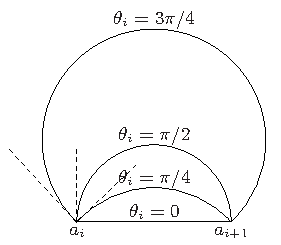
\includegraphics[width=.35\textwidth]{figures/ch08-ex467a.pdf}\end{center}
曲线由 $\theta_1,\ldots,\theta_n$ 完全指定，各角度可在 $(-\pi,\pi)$ 内选择。$\theta_i$ 的选择影响曲线的几种性质，例如总弧长 $L$，以及接点角不连续性，后者描述如下。

在每个 $a_i$、$i=2,\ldots,n-1$ 处，两段圆弧相接，一段从前一点而来，一段通向下一点。若两条切线方向恰好相反，从而曲线在 $a_i$ 处可微，则称该点没有接点角不连续。一般地，将 $a_i$ 处接点角不连续量定义为 $|\theta_{i-1}+\theta_i+\psi_i|$，其中 $\psi_i$ 为线段 $[a_i,a_{i+1}]$ 与 $[a_{i-1},a_i]$ 的夹角，即 $\psi_i=\angle(a_i-a_{i+1},a_{i-1}-a_i)$，如下图。由于各 $a_i$ 已知，角度 $\psi_i$ 也已知。
\begin{center}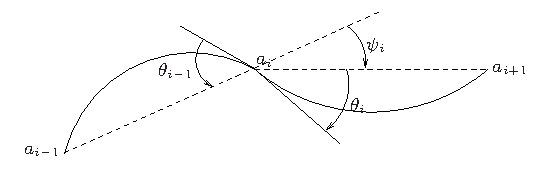
\includegraphics[width=.65\textwidth]{figures/ch08-ex467b.pdf}\end{center}
总接点角不连续量定义为
\[D=\sum_{i=2}^n|\theta_{i-1}+\theta_i+\psi_i|.\]
将最小化总弧长 $L$ 与总接点角不连续量 $D$ 的问题，写成双准则凸优化。说明如何找到最优权衡曲线上的极端点。
% Source PDF page 468 (printed p. 454): blank page in source.


\part{算法}
\chapter{无约束最小化}
% Source PDF page 471 (printed p. 457)
\section{无约束最小化问题}
本章讨论求解无约束优化问题
\begin{equation}
\text{最小化}\quad f(x)\tag{9.1}
\end{equation}
的方法，其中 $f:\R^n\to\R$ 凸且二阶连续可微（因此 $\dom f$ 是开集）。假设问题有解，即存在最优点 $x^\star$。（更准确地说，本章稍后的假设将保证 $x^\star$ 存在且唯一。）用 $p^\star$ 表示最优值 $\inf_xf(x)=f(x^\star)$。

由于 $f$ 可微且凸，点 $x^\star$ 最优的充要条件是
\begin{equation}
\nabla f(x^\star)=0\tag{9.2}
\end{equation}
（见§4.2.3）。因此，求解无约束最小化问题（9.1），等同于求解（9.2），即一组含 $n$ 个变量 $x_1,\ldots,x_n$ 的 $n$ 个方程。少数特殊情形下，可以解析求解最优性方程（9.2），从而得到（9.1）的解；但通常必须用迭代算法。这里指算法计算一列点 $x^{(0)},x^{(1)},\ldots\in\dom f$，使 $k\to\infty$ 时 $f(x^{(k)})\to p^\star$。这样的点列称为问题（9.1）的\emph{极小化序列}。当 $f(x^{(k)})-p^\star\le\epsilon$ 时算法终止，其中 $\epsilon>0$ 为指定容差。

\subsubsection*{初始点与下水平集}
本章的方法需要适当初始点 $x^{(0)}$。初始点必须属于 $\dom f$，而且下水平集
\begin{equation}
S=\{x\in\dom f\mid f(x)\le f(x^{(0)})\}\tag{9.3}
\end{equation}
必须闭。若函数 $f$ 闭，即所有下水平集闭（见§A.3.3），则任意 $x^{(0)}\in\dom f$ 都满足此条件。定义域为 $\R^n$ 的连续函数都是闭函数。

% Source PDF page 472 (printed p. 458)
因此，若 $\dom f=\R^n$，任意 $x^{(0)}$ 都满足初始下水平集条件。另一类重要闭函数是具有开定义域的连续函数，且当 $x$ 趋近 $\operatorname{bd}\dom f$ 时 $f(x)$ 趋于无穷大。

\subsection{例子}
\subsubsection*{二次最小化与最小二乘}
一般凸二次最小化问题形式为
\begin{equation}
\text{最小化}\quad(1/2)x^\T Px+q^\T x+r,\tag{9.4}
\end{equation}
其中 $P\in\mathbf S_+^n$、$q\in\R^n$、$r\in\R$。可通过最优性条件 $Px^\star+q=0$ 求解，这是线性方程组。当 $P\succ0$ 时，解唯一，为 $x^\star=-P^{-1}q$。更一般地，当 $P$ 非正定时，$Px^\star=-q$ 的任意解都是（9.4）的最优解；若该方程无解，则（9.4）无下界（见习题9.1）。能够解析求解二次最小化问题（9.4），是牛顿法的基础；牛顿法是强有力的无约束最小化方法，在§9.5介绍。

二次最小化一个极常见的特殊情形是最小二乘问题
\[
\text{最小化}\quad
\norm{Ax-b}_2^2=x^\T(A^\T A)x-2(A^\T b)^\T x+b^\T b.
\]
其最优性条件
\[
A^\T Ax^\star=A^\T b
\]
称为最小二乘问题的\emph{正规方程}。

\subsubsection*{无约束几何规划}
第二个例子是凸形式的无约束几何规划
\[
\text{最小化}\quad
f(x)=\log\left(\sum_{i=1}^m\exp(a_i^\T x+b_i)\right).
\]
最优性条件为
\[
\nabla f(x^\star)=
\frac1{\sum_{j=1}^m\exp(a_j^\T x^\star+b_j)}
\sum_{i=1}^m\exp(a_i^\T x^\star+b_i)a_i=0.
\]
它通常没有解析解，所以必须采用迭代算法。这个问题的 $\dom f=\R^n$，因此可任选一点作为初始点 $x^{(0)}$。

\subsubsection*{线性不等式的解析中心}
考虑优化问题
\begin{equation}
\text{最小化}\quad
f(x)=-\sum_{i=1}^m\log(b_i-a_i^\T x),\tag{9.5}
\end{equation}

% Source PDF page 473 (printed p. 459)
其中 $f$ 的定义域是开集
\[
\dom f=\{x\mid a_i^\T x<b_i,\ i=1,\ldots,m\}.
\]
该问题的目标函数 $f$ 称为不等式 $a_i^\T x\le b_i$ 的\emph{对数障碍}。问题（9.5）的解若存在，称为这些不等式的\emph{解析中心}。初始点 $x^{(0)}$ 必须满足严格不等式 $a_i^\T x^{(0)}<b_i$，$i=1,\ldots,m$。由于 $f$ 闭，任意这样的点对应的下水平集 $S$ 都闭。

\subsubsection*{线性矩阵不等式的解析中心}
一个密切相关的问题是
\begin{equation}
\text{最小化}\quad f(x)=\log\det F(x)^{-1},\tag{9.6}
\end{equation}
其中 $F:\R^n\to\mathbf S^p$ 仿射，即
\[
F(x)=F_0+x_1F_1+\cdots+x_nF_n,
\]
$F_i\in\mathbf S^p$。这里 $f$ 的定义域为
\[
\dom f=\{x\mid F(x)\succ0\}.
\]
目标函数 $f$ 称为线性矩阵不等式 $F(x)\succeq0$ 的\emph{对数障碍}，其解（若存在）称为该线性矩阵不等式的\emph{解析中心}。初始点 $x^{(0)}$ 必须满足严格线性矩阵不等式 $F(x^{(0)})\succ0$。与前例一样，由于 $f$ 闭，任意这种点的下水平集闭。

\subsection{强凸性及其推论}
本章大部分内容（§9.6除外）假设目标函数在 $S$ 上\emph{强凸}，即存在 $m>0$，使所有 $x\in S$ 都满足
\begin{equation}
\nabla^2 f(x)\succeq mI.\tag{9.7}
\end{equation}
强凸性有几个有趣的推论。对 $x,y\in S$，有
\[
f(y)=f(x)+\nabla f(x)^\T(y-x)
+\tfrac12(y-x)^\T\nabla^2f(z)(y-x),
\]
其中 $z$ 是线段 $[x,y]$ 上的某点。由强凸假设（9.7），右端最后一项至少为 $(m/2)\norm{y-x}_2^2$，所以对所有 $x,y\in S$，
\begin{equation}
f(y)\ge f(x)+\nabla f(x)^\T(y-x)+\frac m2\norm{y-x}_2^2.\tag{9.8}
\end{equation}
当 $m=0$ 时，就得到刻画凸性的基本不等式；$m>0$ 时，得到的 $f(y)$ 下界比单凭凸性得到的更好。

% Source PDF page 474 (printed p. 460)
先说明如何用（9.8）以 $\norm{\nabla f(x)}_2$ 为 $f(x)-p^\star$（即 $x$ 的次优程度）求界。固定 $x$ 后，（9.8）右端是关于 $y$ 的凸二次函数。令关于 $y$ 的梯度为零，可知 $\widetilde y=x-(1/m)\nabla f(x)$ 使右端最小。因此
\[
\begin{aligned}
f(y)&\ge f(x)+\nabla f(x)^\T(y-x)+\frac m2\norm{y-x}_2^2\\
&\ge f(x)+\nabla f(x)^\T(\widetilde y-x)+\frac m2\norm{\widetilde y-x}_2^2\\
&=f(x)-\frac1{2m}\norm{\nabla f(x)}_2^2.
\end{aligned}
\]
由于对任意 $y\in S$ 都成立，故
\begin{equation}
p^\star\ge f(x)-\frac1{2m}\norm{\nabla f(x)}_2^2.\tag{9.9}
\end{equation}
这说明，若某点的梯度很小，该点就接近最优。还可将（9.9）解释为推广最优性条件（9.2）的次优性条件：
\begin{equation}
\norm{\nabla f(x)}_2\le(2m\epsilon)^{1/2}
\ \Longrightarrow\ f(x)-p^\star\le\epsilon.\tag{9.10}
\end{equation}

还能用 $\norm{\nabla f(x)}_2$ 为 $x$ 到任意最优点 $x^\star$ 的距离 $\norm{x-x^\star}_2$ 求界：
\begin{equation}
\norm{x-x^\star}_2\le\frac2m\norm{\nabla f(x)}_2.\tag{9.11}
\end{equation}
在（9.8）中取 $y=x^\star$，有
\[
\begin{aligned}
p^\star=f(x^\star)
&\ge f(x)+\nabla f(x)^\T(x^\star-x)+\frac m2\norm{x^\star-x}_2^2\\
&\ge f(x)-\norm{\nabla f(x)}_2\norm{x^\star-x}_2+\frac m2\norm{x^\star-x}_2^2,
\end{aligned}
\]
第二个不等式利用Cauchy--Schwarz不等式。由于 $p^\star\le f(x)$，必有
\[
-\norm{\nabla f(x)}_2\norm{x^\star-x}_2+\frac m2\norm{x^\star-x}_2^2\le0,
\]
由此得到（9.11）。其一个推论是最优点 $x^\star$ 唯一。

\subsubsection*{$\nabla^2f(x)$ 的上界}
（9.8）意味着包含在 $S$ 中的下水平集有界，特别地，$S$ 本身有界。因此，$\nabla^2f(x)$ 的最大特征值作为 $S$ 上关于 $x$ 的连续函数，在 $S$ 上有上界，即存在常数 $M$，使所有 $x\in S$ 满足
\begin{equation}
\nabla^2f(x)\preceq MI.\tag{9.12}
\end{equation}

% Source PDF page 475 (printed p. 461)
Hessian的这个上界意味着，对于任意 $x,y\in S$，
\begin{equation}
f(y)\le f(x)+\nabla f(x)^\T(y-x)+\frac M2\norm{y-x}_2^2,\tag{9.13}
\end{equation}
它类似于（9.8）。两边对 $y$ 最小化，得到
\begin{equation}
p^\star\le f(x)-\frac1{2M}\norm{\nabla f(x)}_2^2,\tag{9.14}
\end{equation}
对应于（9.9）。

\subsubsection*{下水平集的条件数}
由强凸不等式（9.7）和（9.12），对所有 $x\in S$，
\begin{equation}
mI\preceq\nabla^2f(x)\preceq MI.\tag{9.15}
\end{equation}
比值 $\kappa=M/m$ 因而是矩阵 $\nabla^2f(x)$ 的条件数（最大特征值与最小特征值之比）的上界。还可用 $f$ 的下水平集为（9.15）给出几何解释。

对凸集 $C\subseteq\R^n$，定义其沿方向 $q$（$\norm q_2=1$）的\emph{宽度}为
\[
W(C,q)=\sup_{z\in C}q^\T z-\inf_{z\in C}q^\T z.
\]
$C$ 的最小和最大宽度为
\[
W_{\min}=\inf_{\norm q_2=1}W(C,q),\qquad
W_{\max}=\sup_{\norm q_2=1}W(C,q).
\]
凸集 $C$ 的\emph{条件数}定义为
\[
\operatorname{cond}(C)=\frac{W_{\max}^2}{W_{\min}^2},
\]
即最大宽度与最小宽度之比的平方。$C$ 的条件数衡量其各向异性或偏心程度。条件数小（例如接近1），表示集合在各方向的宽度大致相同，即接近球形；条件数大，则表示某些方向远比其他方向宽。

\begin{origexample}{9.1}
\emph{椭球的条件数。}设椭球
\[
\mathcal E=\{x\mid(x-x_0)^\T A^{-1}(x-x_0)\le1\},
\]
其中 $A\in\mathbf S_{++}^n$。$\mathcal E$ 沿 $q$ 方向的宽度为
\[
\begin{aligned}
\sup_{z\in\mathcal E}q^\T z-\inf_{z\in\mathcal E}q^\T z
&=(\norm{A^{1/2}q}_2+q^\T x_0)-(-\norm{A^{1/2}q}_2+q^\T x_0)\\
&=2\norm{A^{1/2}q}_2.
\end{aligned}
\]

% Source PDF page 476 (printed p. 462)
所以其最小、最大宽度为
\[
W_{\min}=2\lambda_{\min}(A)^{1/2},\qquad
W_{\max}=2\lambda_{\max}(A)^{1/2},
\]
条件数为
\[
\operatorname{cond}(\mathcal E)
=\frac{\lambda_{\max}(A)}{\lambda_{\min}(A)}=\kappa(A),
\]
其中 $\kappa(A)$ 为矩阵 $A$ 的条件数，即最大奇异值与最小奇异值之比。因此椭球 $\mathcal E$ 的条件数与定义它的矩阵 $A$ 的条件数相同。
\end{origexample}

现设对所有 $x\in S$，有 $mI\preceq\nabla^2f(x)\preceq MI$。为 $\alpha$ 下水平集 $C_\alpha=\{x\mid f(x)\le\alpha\}$ 的条件数求界，其中 $p^\star<\alpha\le f(x^{(0)})$。在（9.13）、（9.8）中取 $x=x^\star$，有
\[
p^\star+(M/2)\norm{y-x^\star}_2^2\ge f(y)
\ge p^\star+(m/2)\norm{y-x^\star}_2^2.
\]
这意味着 $B_{\mathrm{inner}}\subseteq C_\alpha\subseteq B_{\mathrm{outer}}$，其中
\[
\begin{aligned}
B_{\mathrm{inner}}&=\{y\mid\norm{y-x^\star}_2\le(2(\alpha-p^\star)/M)^{1/2}\},\\
B_{\mathrm{outer}}&=\{y\mid\norm{y-x^\star}_2\le(2(\alpha-p^\star)/m)^{1/2}\}.
\end{aligned}
\]
换言之，$\alpha$ 下水平集包含球 $B_{\mathrm{inner}}$，并包含在球 $B_{\mathrm{outer}}$ 内，两球半径分别为
\[
(2(\alpha-p^\star)/M)^{1/2},\qquad(2(\alpha-p^\star)/m)^{1/2}.
\]
半径比的平方给出 $C_\alpha$ 条件数的上界：
\[
\operatorname{cond}(C_\alpha)\le M/m.
\]

还可为最优点处Hessian的条件数 $\kappa(\nabla^2f(x^\star))$ 给出几何解释。从 $f$ 在 $x^\star$ 附近的Taylor展开，
\[
f(y)\approx p^\star+\tfrac12(y-x^\star)^\T\nabla^2f(x^\star)(y-x^\star),
\]
可知 $\alpha$ 接近 $p^\star$ 时，
\[
C_\alpha\approx\{y\mid(y-x^\star)^\T\nabla^2f(x^\star)(y-x^\star)
\le2(\alpha-p^\star)\},
\]
即下水平集可由中心为 $x^\star$ 的椭球很好地近似。因此
\[
\lim_{\alpha\to p^\star}\operatorname{cond}(C_\alpha)=\kappa(\nabla^2f(x^\star)).
\]
将会看到，$f$ 下水平集的条件数（上界为 $M/m$）强烈影响某些常见无约束最小化方法的效率。

% Source PDF page 477 (printed p. 463)
\subsubsection*{强凸性常数}
必须记住，只有少数情况下才知道常数 $m,M$，因此（9.10）不能作为实际停止准则。它可以视为概念上的停止准则：若 $f$ 在 $x$ 的梯度足够小，则 $f(x)$ 与 $p^\star$ 之差就小。若在 $\norm{\nabla f(x^{(k)})}_2\le\eta$ 时停止算法，其中 $\eta$ 选得足够小，（很可能）小于 $(m\epsilon)^{1/2}$，那么就（很可能）有 $f(x^{(k)})-p^\star\le\epsilon$。

后面各节将给出算法的收敛证明，其中包含达到 $f(x^{(k)})-p^\star\le\epsilon$ 所需迭代次数的界，$\epsilon$ 为正容差。许多界涉及通常未知的常数 $m,M$，因此同样适用上述讨论。这些结果至少在概念上有用：它们确立算法收敛，尽管达到给定精度所需次数的界依赖未知常数。

我们将遇到一个重要例外。§9.6研究一类特殊凸函数，称为\emph{自协调函数}。对这些函数，可以给出不依赖任何未知常数的完整牛顿法收敛分析。

\section{下降方法}
本章算法产生极小化序列 $x^{(k)}$，$k=1,\ldots$，其中
\[
x^{(k+1)}=x^{(k)}+t^{(k)}\Delta x^{(k)},
\]
并且除非 $x^{(k)}$ 已最优，否则 $t^{(k)}>0$。这里，将 $\Delta$ 和 $x$ 连写的记号 $\Delta x$ 应视为一个整体，是 $\R^n$ 中的向量，称为\emph{步}或\emph{搜索方向}（虽然它不必有单位范数）；$k=0,1,\ldots$ 为迭代次数。标量 $t^{(k)}\ge0$ 称为第 $k$ 次迭代的\emph{步长}（虽然除非 $\norm{\Delta x^{(k)}}=1$，它并不等于 $\norm{x^{(k+1)}-x^{(k)}}$）。“搜索步”和“缩放因子”更准确，但广泛使用的术语是“搜索方向”和“步长”。只关注单次迭代时，有时省去上标，以较简洁的 $x^+=x+t\Delta x$ 或 $x:=x+t\Delta x$ 代替 $x^{(k+1)}=x^{(k)}+t^{(k)}\Delta x^{(k)}$。

研究的所有方法都是\emph{下降方法}，即除非 $x^{(k)}$ 最优，否则
\[
f(x^{(k+1)})<f(x^{(k)}).
\]
这说明对所有 $k$，$x^{(k)}\in S$，特别地，$x^{(k)}\in\dom f$。由凸性，$\nabla f(x^{(k)})^\T(y-x^{(k)})\ge0$ 蕴含 $f(y)\ge f(x^{(k)})$，因此下降方法的搜索方向必满足
\[
\nabla f(x^{(k)})^\T\Delta x^{(k)}<0,
\]
即与负梯度成锐角。这样的方向称为（$f$ 在 $x^{(k)}$ 处的）\emph{下降方向}。

% Source PDF page 478 (printed p. 464)
一般下降方法的框架如下，交替执行两步：确定下降方向 $\Delta x$ 和选择步长 $t$。

\begin{origalgorithm}{9.1}
\emph{一般下降方法。}

给定初始点 $x\in\dom f$。

重复：
\begin{enumerate}
\item 确定下降方向 $\Delta x$。
\item \emph{线搜索。}选择步长 $t>0$。
\item \emph{更新。}$x:=x+t\Delta x$。
\end{enumerate}
直到满足停止准则。
\end{origalgorithm}

第二步称为\emph{线搜索}，因为步长 $t$ 的选择决定下一迭代点在线 $\{x+t\Delta x\mid t\in\R_+\}$ 上的位置。（更准确的术语或许是“射线搜索”。）

实际下降方法具有同样框架，但组织方式可能不同。例如，停止准则常在计算下降方向 $\Delta x$ 时或计算后立即检查。如次优性条件（9.9）所示，停止准则常用 $\norm{\nabla f(x)}_2\le\eta$，其中 $\eta$ 是很小的正数。

\subsubsection*{精确线搜索}
实践中有时使用\emph{精确线搜索}，选取 $t$ 使 $f$ 沿射线 $\{x+t\Delta x\mid t\ge0\}$ 最小：
\begin{equation}
t=\argmin_{s\ge0}f(x+s\Delta x).\tag{9.16}
\end{equation}
当（9.16）所需单变量最小化问题的代价远小于搜索方向本身的计算代价时，会使用精确线搜索。有些特殊情形下可解析求得射线上的最小点，另一些情形则能高效数值求解（§9.7.1讨论）。

\subsubsection*{回溯线搜索}
实践中使用的大多数线搜索都是\emph{非精确}的：选择近似最小化射线 $\{x+t\Delta x\mid t\ge0\}$ 上 $f$ 的步长，甚至仅使 $f$ “充分”减小。已提出许多非精确线搜索方法。\emph{回溯线搜索}是一种非常简单且有效的方法，依赖两个常数 $\alpha,\beta$，满足 $0<\alpha<0.5$、$0<\beta<1$。

\begin{origalgorithm}{9.2}
\emph{回溯线搜索。}

给定 $f$ 在 $x\in\dom f$ 处的下降方向 $\Delta x$，以及 $\alpha\in(0,0.5)$、$\beta\in(0,1)$。
\[
t:=1.
\]
只要 $f(x+t\Delta x)>f(x)+\alpha t\nabla f(x)^\T\Delta x$，就重复令 $t:=\beta t$。
\end{origalgorithm}

% Source PDF page 479 (printed p. 465)
\begin{figure}[htbp]\centering
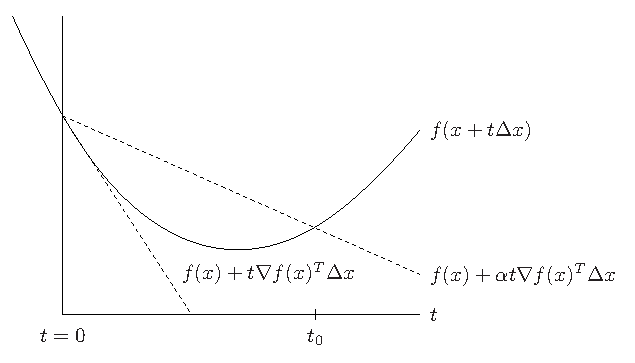
\includegraphics[width=.8\linewidth]{figures/ch09-fig01.pdf}
\caption*{图9.1\quad 回溯线搜索。曲线表示将 $f$ 限制在搜索直线上得到的函数。较低虚线为 $f$ 的线性外推，较高虚线的斜率缩小为其 $\alpha$ 倍。回溯条件要求 $f$ 位于较高虚线下方，即 $0\le t\le t_0$。}
\end{figure}
称为回溯，是因为线搜索从单位步长开始，每次将其乘 $\beta$ 缩小，直到满足停止条件 $f(x+t\Delta x)\le f(x)+\alpha t\nabla f(x)^\T\Delta x$。由于 $\Delta x$ 是下降方向，有 $\nabla f(x)^\T\Delta x<0$，所以 $t$ 足够小时，
\[
f(x+t\Delta x)\approx f(x)+t\nabla f(x)^\T\Delta x
<f(x)+\alpha t\nabla f(x)^\T\Delta x,
\]
这说明回溯线搜索最终会终止。常数 $\alpha$ 可理解为我们接受的函数减小量占线性外推所预测减小量的比例。（要求 $\alpha<0.5$ 的原因稍后会清楚。）

图9.1说明回溯条件。由图可见，而且可以证明，对 $t\ge0$，回溯退出不等式
$f(x+t\Delta x)\le f(x)+\alpha t\nabla f(x)^\T\Delta x$
在区间 $(0,t_0]$ 上成立。因此回溯会以满足
\[
t=1,\qquad\text{或}\qquad t\in(\beta t_0,t_0]
\]
的步长停止。第一种情况发生于 $t=1$ 满足回溯条件时，即 $1\le t_0$。特别地，回溯线搜索所得步长满足
\[
t\ge\min\{1,\beta t_0\}.
\]
当 $\dom f$ 不是整个 $\R^n$ 时，必须谨慎理解回溯中的条件
$f(x+t\Delta x)\le f(x)+\alpha t\nabla f(x)^\T\Delta x$。
按照函数在定义域之外取无穷大的约定，这个不等式蕴含 $x+t\Delta x\in\dom f$。实际实现时，先反复将 $t$ 乘 $\beta$，直到 $x+t\Delta x\in\dom f$。

% Source PDF page 480 (printed p. 466)
然后再开始检查 $f(x+t\Delta x)\le f(x)+\alpha t\nabla f(x)^\T\Delta x$ 是否成立。

参数 $\alpha$ 通常选在0.01至0.3之间，即接受的 $f$ 减小量为线性外推预测值的1\%至30\%。$\beta$ 常选在0.1（相当粗略的搜索）至0.8（较细的搜索）之间。

\section{梯度下降法}
搜索方向的自然选择是负梯度 $\Delta x=-\nabla f(x)$。所得算法称为\emph{梯度算法}或\emph{梯度下降法}。

\begin{origalgorithm}{9.3}
\emph{梯度下降法。}

给定初始点 $x\in\dom f$。

重复：
\begin{enumerate}
\item $\Delta x:=-\nabla f(x)$。
\item \emph{线搜索。}通过精确或回溯线搜索选择步长 $t$。
\item \emph{更新。}$x:=x+t\Delta x$。
\end{enumerate}
直到满足停止准则。
\end{origalgorithm}

停止准则通常为 $\norm{\nabla f(x)}_2\le\eta$，其中 $\eta$ 为很小的正数。多数实现中，在步骤1之后检查这一条件，而非在更新之后。

\subsection{收敛分析}
本节给出梯度法的简单收敛分析。以简洁记号 $x^+=x+t\Delta x$ 代替
$x^{(k+1)}=x^{(k)}+t^{(k)}\Delta x^{(k)}$，其中 $\Delta x=-\nabla f(x)$。假设 $f$ 在 $S$ 上强凸，因此存在正常数 $m,M$，使所有 $x\in S$ 满足 $mI\preceq\nabla^2f(x)\preceq MI$。定义 $\widetilde f:\R\to\R$ 为
$\widetilde f(t)=f(x-t\nabla f(x))$，即 $f$ 沿负梯度方向关于步长 $t$ 的函数。以下仅考虑满足 $x-t\nabla f(x)\in S$ 的 $t$。在（9.13）中取 $y=x-t\nabla f(x)$，得到 $\widetilde f$ 的二次上界：
\begin{equation}
\widetilde f(t)\le f(x)-t\norm{\nabla f(x)}_2^2
+\frac{Mt^2}{2}\norm{\nabla f(x)}_2^2.\tag{9.17}
\end{equation}

\subsubsection*{精确线搜索的分析}
假设使用精确线搜索，在（9.17）两边对 $t$ 最小化。左端得到 $\widetilde f(t_{\mathrm{exact}})$，其中 $t_{\mathrm{exact}}$ 是

% Source PDF page 481 (printed p. 467)
最小化 $\widetilde f$ 的步长。右端是简单二次函数，在 $t=1/M$ 时最小，最小值为 $f(x)-(1/(2M))\norm{\nabla f(x)}_2^2$。因此
\[
f(x^+)=\widetilde f(t_{\mathrm{exact}})
\le f(x)-\frac1{2M}\norm{\nabla f(x)}_2^2.
\]
两边减 $p^\star$，得到
\[
f(x^+)-p^\star\le f(x)-p^\star-\frac1{2M}\norm{\nabla f(x)}_2^2.
\]
结合（9.9）给出的 $\norm{\nabla f(x)}_2^2\ge2m(f(x)-p^\star)$，可得
\[
f(x^+)-p^\star\le(1-m/M)(f(x)-p^\star).
\]
递归应用，得到
\begin{equation}
f(x^{(k)})-p^\star\le c^k(f(x^{(0)})-p^\star),\tag{9.18}
\end{equation}
其中 $c=1-m/M<1$。因此 $k\to\infty$ 时 $f(x^{(k)})\to p^\star$。特别地，采用精确线搜索的梯度法，至多经过
\begin{equation}
\frac{\log((f(x^{(0)})-p^\star)/\epsilon)}{\log(1/c)}\tag{9.19}
\end{equation}
次迭代，就有 $f(x^{(k)})-p^\star\le\epsilon$。

虽然迭代次数的这一界较粗，但能帮助理解梯度法。分子
\[
\log((f(x^{(0)})-p^\star)/\epsilon)
\]
可解释为初始次优程度（$f(x^{(0)})$ 与 $p^\star$ 的间隙）与最终次优程度（小于 $\epsilon$）之比的对数。这提示迭代次数依赖初始点的好坏和最终所需精度。

界（9.19）的分母 $\log(1/c)$ 是 $M/m$ 的函数；已知 $M/m$ 是 $S$ 上 $\nabla^2f(x)$ 条件数的界，也是下水平集 $\{z\mid f(z)\le\alpha\}$ 条件数的界。当条件数界 $M/m$ 很大时，
\[
\log(1/c)=-\log(1-m/M)\approx m/M,
\]
所以迭代次数的界随 $M/m$ 增大而近似线性增长。

将会看到，若 $f$ 的Hessian在 $x^\star$ 附近条件数大，梯度法确实需要很多次迭代。反之，若 $f$ 的下水平集比较各向同性，使条件数界 $M/m$ 可取得较小，（9.18）说明收敛很快，因为 $c$ 小，至少不会太接近1。

（9.18）说明误差 $f(x^{(k)})-p^\star$ 至少像等比数列一样快地收敛于零。在迭代数值方法中，这称为\emph{线性收敛}，因为在误差对迭代次数的对数—线性图上，误差位于一条直线下方。

% Source PDF page 482 (printed p. 468)
\subsubsection*{回溯线搜索的分析}
再考虑梯度下降法采用回溯线搜索的情形。下面证明，凡 $0\le t\le1/M$，回溯退出条件
\[
\widetilde f(t)\le f(x)-\alpha t\norm{\nabla f(x)}_2^2
\]
都成立。首先注意
\[
0\le t\le1/M\ \Longrightarrow\ -t+\frac{Mt^2}{2}\le-t/2,
\]
这由 $-t+Mt^2/2$ 的凸性得到。结合界（9.17），对 $0\le t\le1/M$，
\[
\begin{aligned}
\widetilde f(t)&\le f(x)-t\norm{\nabla f(x)}_2^2
+\frac{Mt^2}{2}\norm{\nabla f(x)}_2^2\\
&\le f(x)-(t/2)\norm{\nabla f(x)}_2^2\\
&\le f(x)-\alpha t\norm{\nabla f(x)}_2^2,
\end{aligned}
\]
最后一步利用 $\alpha<1/2$。因此回溯线搜索终止时，或者 $t=1$，或者 $t\ge\beta/M$。由此得到目标减小量的下界。第一种情况下，
\[
f(x^+)\le f(x)-\alpha\norm{\nabla f(x)}_2^2;
\]
第二种情况下，
\[
f(x^+)\le f(x)-(\beta\alpha/M)\norm{\nabla f(x)}_2^2.
\]
综合起来，总有
\[
f(x^+)\le f(x)-\min\{\alpha,\beta\alpha/M\}\norm{\nabla f(x)}_2^2.
\]
接下来与精确线搜索完全一样。两边减 $p^\star$，得到
\[
f(x^+)-p^\star\le f(x)-p^\star
-\min\{\alpha,\beta\alpha/M\}\norm{\nabla f(x)}_2^2,
\]
结合 $\norm{\nabla f(x)}_2^2\ge2m(f(x)-p^\star)$，得到
\[
f(x^+)-p^\star
\le(1-\min\{2m\alpha,2\beta\alpha m/M\})(f(x)-p^\star).
\]
因此
\[
f(x^{(k)})-p^\star\le c^k(f(x^{(0)})-p^\star),
\]
其中
\[
c=1-\min\{2m\alpha,2\beta\alpha m/M\}<1.
\]
特别地，$f(x^{(k)})$ 至少与一个等比数列一样快地收敛于 $p^\star$，其指数至少部分取决于条件数界 $M/m$。用迭代方法术语说，收敛至少是线性的。

% Source PDF page 483 (printed p. 469)
\begin{figure}[htbp]\centering
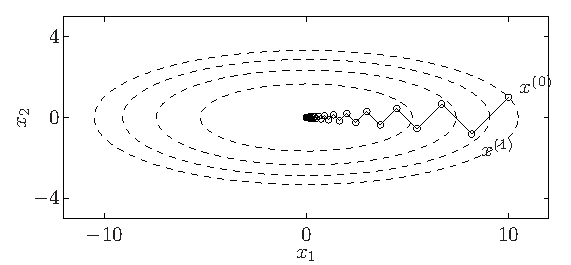
\includegraphics[width=.75\linewidth]{figures/ch09-fig02.pdf}
\caption*{图9.2\quad 函数 $f(x)=(1/2)(x_1^2+10x_2^2)$ 的若干等值线。其下水平集为椭球，条件数恰为10。图中显示从 $x^{(0)}=(10,1)$ 出发，采用精确线搜索的梯度法迭代点。}
\end{figure}
\subsection{例子}
\subsubsection*{$\R^2$ 中的二次问题}
第一个例子非常简单。考虑 $\R^2$ 上的二次目标函数
\[
f(x)=\tfrac12(x_1^2+\gamma x_2^2),
\]
其中 $\gamma>0$。显然，最优点为 $x^\star=0$，最优值为0。$f$ 的Hessian为常矩阵，特征值为1和 $\gamma$，因此所有下水平集的条件数都恰为
\[
\frac{\max\{1,\gamma\}}{\min\{1,\gamma\}}=\max\{\gamma,1/\gamma\}.
\]
强凸性常数 $m,M$ 最紧的选择为
\[
m=\min\{1,\gamma\},\qquad M=\max\{1,\gamma\}.
\]
从 $x^{(0)}=(\gamma,1)$ 出发，应用采用精确线搜索的梯度下降法。此时可求得迭代点 $x^{(k)}$ 及函数值的闭式表达式（习题9.6）：
\[
x_1^{(k)}=\gamma\left(\frac{\gamma-1}{\gamma+1}\right)^k,\qquad
x_2^{(k)}=\left(-\frac{\gamma-1}{\gamma+1}\right)^k,
\]
以及
\[
f(x^{(k)})=\frac{\gamma(\gamma+1)}2
\left(\frac{\gamma-1}{\gamma+1}\right)^{2k}
=\left(\frac{\gamma-1}{\gamma+1}\right)^{2k}f(x^{(0)}).
\]
图9.2显示 $\gamma=10$ 的情形。

这个简单例子的收敛恰为线性，即误差恰好构成等比数列，每次迭代乘以因子 $|(\gamma-1)/(\gamma+1)|^2$。

% Source PDF page 484 (printed p. 470)
$\gamma=1$ 时，一次迭代即得精确解；$\gamma$ 离1不远时（例如介于 $1/3$ 与3之间），收敛很快；$\gamma\gg1$ 或 $\gamma\ll1$ 时，收敛很慢。

可将收敛与§9.3.1所得界比较。取最不保守的 $m=\min\{1,\gamma\}$、$M=\max\{1,\gamma\}$，界（9.18）保证每次迭代误差至少缩小到原来的 $c=1-m/M$。实际上，误差每次恰好乘以
\[
\left(\frac{1-m/M}{1+m/M}\right)^2.
\]
对于对应大条件数的很小 $m/M$，上界（9.19）说明达到给定精度所需迭代次数至多按 $M/m$ 增长。本例中，实际次数近似按 $(M/m)/4$ 增长，即约为上界的四分之一。因此，对于这一简单例子，简单分析得到的迭代次数界只保守约四倍（采用最不保守的 $m,M$）。特别地，收敛速率及其上界都强烈依赖下水平集的条件数。

\subsubsection*{$\R^2$ 中的非二次问题}
再考虑 $\R^2$ 中非二次例子：
\begin{equation}
f(x_1,x_2)=e^{x_1+3x_2-0.1}
+e^{x_1-3x_2-0.1}+e^{-x_1-0.1}.\tag{9.20}
\end{equation}
采用回溯线搜索的梯度法，参数为 $\alpha=0.1,\beta=0.7$。图9.3显示 $f$ 的若干等值线和梯度法产生的迭代点 $x^{(k)}$（小圆圈）。连接相邻迭代点的线表示缩放后的步：
\[
x^{(k+1)}-x^{(k)}=-t^{(k)}\nabla f(x^{(k)}).
\]
图9.4显示误差 $f(x^{(k)})-p^\star$ 与迭代次数 $k$ 的关系。图表明误差近似按等比数列收敛于零，即近似线性收敛。本例中，误差在20次迭代内从约10降到约 $10^{-7}$，所以每次约乘 $10^{-8/20}\approx0.4$。我们的分析预见这种较快收敛，因为 $f$ 的下水平集条件不算太差，即 $M/m$ 可选得不太大。

为比较回溯与精确线搜索，在同一问题、同一初始点上使用精确线搜索的梯度法。结果见图9.5和9.4。收敛也近似线性，速率约为回溯线搜索梯度法的两倍。精确线搜索时，误差在15次迭代中约乘 $10^{-11}$，即每次约乘 $10^{-11/15}\approx0.2$。

% Source PDF page 485 (printed p. 471)
\begin{figure}[htbp]\centering
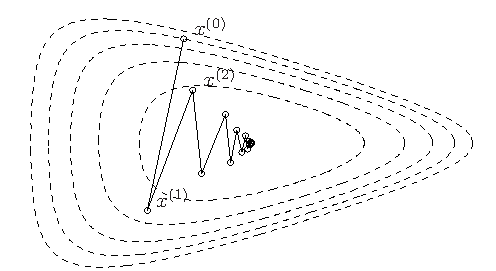
\includegraphics[width=.65\linewidth]{figures/ch09-fig03.pdf}
\caption*{图9.3\quad 采用回溯线搜索的梯度法的迭代点，目标为（9.20）的 $\R^2$ 问题。虚线为 $f$ 的等值线，小圆圈为迭代点。连接相邻迭代点的实线表示缩放后的步 $t^{(k)}\Delta x^{(k)}$。}
\end{figure}
\begin{figure}[htbp]\centering
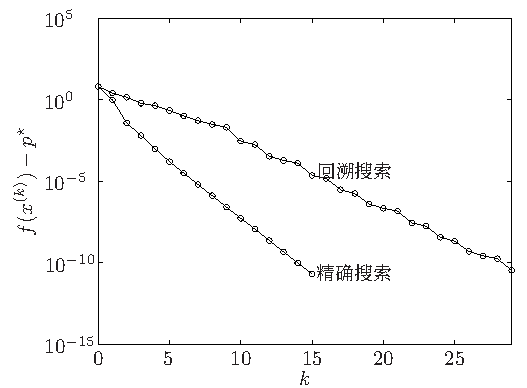
\includegraphics[width=.7\linewidth]{figures/ch09-fig04.pdf}
\caption*{图9.4\quad 对目标为（9.20）的 $\R^2$ 问题，回溯与精确线搜索梯度法的误差 $f(x^{(k)})-p^\star$ 随迭代次数 $k$ 的变化。图中近似线性收敛，回溯线搜索时误差每次迭代约乘0.4，精确线搜索时约乘0.2。}
\end{figure}

% Source PDF page 486 (printed p. 472)
\begin{figure}[htbp]\centering
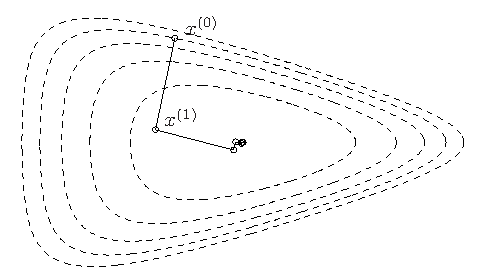
\includegraphics[width=.65\linewidth]{figures/ch09-fig05.pdf}
\caption*{图9.5\quad 对目标为（9.20）的 $\R^2$ 问题，采用精确线搜索的梯度法迭代点。}
\end{figure}
\subsubsection*{$\R^{100}$ 中的问题}
接着考虑较大例子，形式为
\begin{equation}
f(x)=c^\T x-\sum_{i=1}^m\log(b_i-a_i^\T x),\tag{9.21}
\end{equation}
有 $m=500$ 项、$n=100$ 个变量。

参数 $\alpha=0.1,\beta=0.5$ 的回溯线搜索梯度法的进展见图9.6。开始约20次迭代近似线性且较快收敛，随后转为较慢的线性收敛。总体而言，约175次迭代将误差缩小 $10^6$ 倍，平均每次误差约乘 $10^{-6/175}\approx0.92$。前20次的初始收敛率约为每次乘0.8；20次以后较慢的最终收敛率约为每次乘0.94。

图9.6还显示精确线搜索梯度法的收敛。仍近似线性，总体误差每次约乘 $10^{-6/140}\approx0.91$，只比回溯线搜索略快。

最后考察回溯参数 $\alpha,\beta$ 对收敛速率的影响，统计达到 $f(x^{(k)})-p^\star\le10^{-5}$ 所需迭代次数。第一个实验固定 $\beta=0.5$，将 $\alpha$ 从0.05变到0.5。所需次数从较大 $\alpha$（0.2--0.5）时的约80次，到较小 $\alpha$ 时的约170次。这些及其他实验表明，梯度法使用0.2--0.5间较大的 $\alpha$ 效果更好。

类似地，固定 $\alpha=0.1$，将 $\beta$ 从0.05变到0.95，可研究 $\beta$ 的影响。总次数变化同样不大，从 $\beta\approx0.5$ 时约80次，到 $\beta$ 很小或接近1时约200次。这些及其他实验表明，$\beta\approx0.5$ 是不错的选择。

% Source PDF page 487 (printed p. 473)
\begin{figure}[htbp]\centering
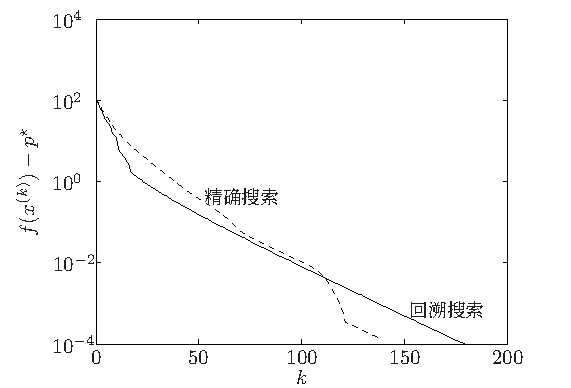
\includegraphics[width=.75\linewidth]{figures/ch09-fig06.pdf}
\caption*{图9.6\quad 对 $\R^{100}$ 中的一个问题，采用回溯和精确线搜索的梯度法误差 $f(x^{(k)})-p^\star$ 随迭代次数 $k$ 的变化。}
\end{figure}
这些实验表明，回溯参数对收敛的影响不大，约不超过两倍。

\subsubsection*{梯度法与条件数}
最后一个实验说明 $\nabla^2f(x)$（或下水平集）条件数对梯度法收敛速率的重要性。以（9.21）的函数开始，但用 $x=T\overline x$ 替换变量 $x$，其中
\[
T=\diag(1,\gamma^{1/n},\gamma^{2/n},\ldots,\gamma^{(n-1)/n}),
\]
即最小化
\begin{equation}
\overline f(\overline x)=c^\T T\overline x
-\sum_{i=1}^m\log(b_i-a_i^\T T\overline x).\tag{9.22}
\end{equation}
这给出以 $\gamma$ 为参数的一族优化问题，$\gamma$ 影响问题条件数。

图9.7显示采用 $\alpha=0.3,\beta=0.7$ 的回溯线搜索时，达到
$\overline f(\overline x^{(k)})-\overline p^\star<10^{-5}$ 所需次数关于 $\gamma$ 的函数。即使对角缩放仅为10:1（$\gamma=10$），次数也超过一千；对角缩放达到20或更大时，梯度法就慢到基本无法使用。

图9.8显示最优点处Hessian $\nabla^2\overline f(\overline x^\star)$ 的条件数。$\gamma$ 很大或很小时，条件数约按 $\max\{\gamma^2,1/\gamma^2\}$ 增长，与迭代次数关于 $\gamma$ 的关系非常相似。这再次说明，条件与收敛速度之间的关系是实际现象，而非分析造成的假象。

% Source PDF page 488 (printed p. 474)
\begin{figure}[htbp]\centering
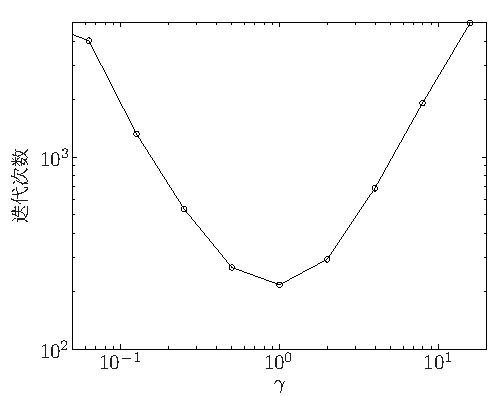
\includegraphics[width=.65\linewidth]{figures/ch09-fig07.pdf}
\caption*{图9.7\quad 梯度法用于（9.22）时的迭代次数。纵轴为达到 $\overline f(\overline x^{(k)})-\overline p^\star<10^{-5}$ 所需次数，横轴为控制对角缩放程度的参数 $\gamma$。采用 $\alpha=0.3,\beta=0.7$ 的回溯线搜索。}
\end{figure}
\begin{figure}[htbp]\centering
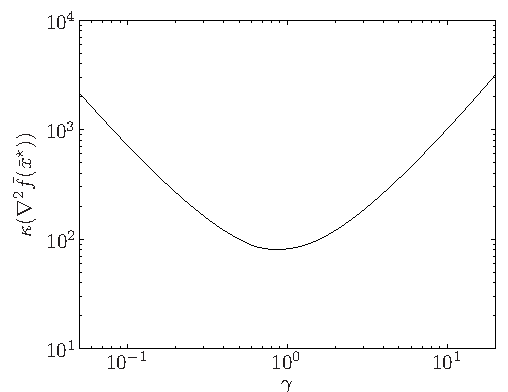
\includegraphics[width=.65\linewidth]{figures/ch09-fig08.pdf}
\caption*{图9.8\quad 函数最小点处Hessian条件数关于 $\gamma$ 的函数。与图9.7比较可见，条件数对收敛速率有很强的影响。}
\end{figure}

% Source PDF page 489 (printed p. 475)
\subsubsection*{结论}
根据上述及其他数值例子，可归纳以下结论。
\begin{itemize}
\item 梯度法常表现出近似线性收敛，即误差 $f(x^{(k)})-p^\star$ 近似按等比数列收敛于零。
\item 回溯参数 $\alpha,\beta$ 的选择对收敛有可察觉但不剧烈的影响。精确线搜索有时改善梯度法收敛，但影响不大（可能不值得为此专门实现精确线搜索）。
\item 收敛速率强烈依赖Hessian或下水平集的条件数。即使问题条件尚可（如条件数为几百），收敛也可能很慢。条件数更大（如1000或以上）时，梯度法慢到实践中无法使用。
\end{itemize}
梯度法的主要优点是简单，主要缺点则是收敛速率对Hessian或下水平集条件数过于敏感。

\section{最速下降法}
$f(x+v)$ 在 $x$ 附近的一阶Taylor近似为
\[
f(x+v)\approx\widehat f(x+v)=f(x)+\nabla f(x)^\T v.
\]
右端第二项 $\nabla f(x)^\T v$ 是 $f$ 在 $x$ 处沿 $v$ 的方向导数，给出小步 $v$ 引起的函数近似变化。若方向导数为负，$v$ 就是下降方向。

现讨论如何选择 $v$，使方向导数尽可能负。由于 $\nabla f(x)^\T v$ 关于 $v$ 线性，只要 $v$ 是下降方向，即 $\nabla f(x)^\T v<0$，就可以将 $v$ 放大，使方向导数任意负。为使问题合理，必须限制 $v$ 的大小，或用其长度归一化。

设 $\norm{\cdot}$ 为 $\R^n$ 的任意范数。定义相对于此范数的\emph{归一化最速下降方向}为
\begin{equation}
\Delta x_{\mathrm{nsd}}=
\argmin\{\nabla f(x)^\T v\mid\norm v=1\}.\tag{9.23}
\end{equation}
（称“一个”最速下降方向，因为可能有多个最小点。）归一化最速下降方向 $\Delta x_{\mathrm{nsd}}$ 是单位范数的步，使 $f$ 的线性近似下降最多。

其几何解释如下。也可将 $\Delta x_{\mathrm{nsd}}$ 定义为
\[
\Delta x_{\mathrm{nsd}}=
\argmin\{\nabla f(x)^\T v\mid\norm v\le1\},
\]

% Source PDF page 490 (printed p. 476)
即范数 $\norm{\cdot}$ 的单位球内，沿 $-\nabla f(x)$ 方向延伸最远的方向。

将归一化方向按特定方式缩放，考虑未归一化的\emph{最速下降步} $\Delta x_{\mathrm{sd}}$ 也很方便：
\begin{equation}
\Delta x_{\mathrm{sd}}=\norm{\nabla f(x)}_*\Delta x_{\mathrm{nsd}},\tag{9.24}
\end{equation}
其中 $\norm{\cdot}_*$ 表示对偶范数。注意，最速下降步满足
\[
\nabla f(x)^\T\Delta x_{\mathrm{sd}}
=\norm{\nabla f(x)}_*\nabla f(x)^\T\Delta x_{\mathrm{nsd}}
=-\norm{\nabla f(x)}_*^2
\]
（见习题9.7）。最速下降法以最速下降方向为搜索方向。

\begin{origalgorithm}{9.4}
\emph{最速下降法。}

给定初始点 $x\in\dom f$。

重复：
\begin{enumerate}
\item 计算最速下降方向 $\Delta x_{\mathrm{sd}}$。
\item \emph{线搜索。}通过回溯或精确线搜索选择 $t$。
\item \emph{更新。}$x:=x+t\Delta x_{\mathrm{sd}}$。
\end{enumerate}
直到满足停止准则。
\end{origalgorithm}

使用精确线搜索时，方向中的缩放因子不影响结果，因此可使用归一化或未归一化方向。

\subsection{欧几里得范数和二次范数下的最速下降}
\subsubsection*{欧几里得范数下的最速下降}
若 $\norm{\cdot}$ 取欧几里得范数，最速下降方向就是负梯度，即 $\Delta x_{\mathrm{sd}}=-\nabla f(x)$。欧几里得范数下的最速下降法与梯度下降法一致。

\subsubsection*{二次范数下的最速下降}
考虑二次范数
\[
\norm z_P=(z^\T Pz)^{1/2}=\norm{P^{1/2}z}_2,
\]
其中 $P\in\mathbf S_{++}^n$。归一化最速下降方向为
\[
\Delta x_{\mathrm{nsd}}
=-\bigl(\nabla f(x)^\T P^{-1}\nabla f(x)\bigr)^{-1/2}P^{-1}\nabla f(x).
\]
对偶范数为 $\norm z_*=\norm{P^{-1/2}z}_2$，所以相对于 $\norm{\cdot}_P$ 的最速下降步为
\begin{equation}
\Delta x_{\mathrm{sd}}=-P^{-1}\nabla f(x).\tag{9.25}
\end{equation}
图9.9说明二次范数的归一化最速下降方向。

% Source PDF page 491 (printed p. 477)
\begin{figure}[htbp]\centering
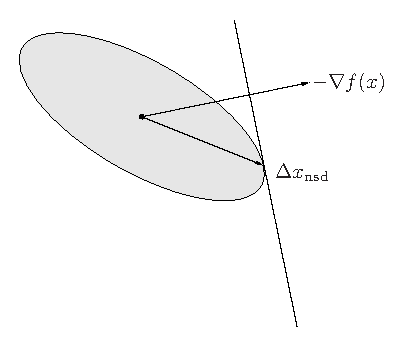
\includegraphics[width=.55\linewidth]{figures/ch09-fig09.pdf}
\caption*{图9.9\quad 二次范数的归一化最速下降方向。椭球是该范数的单位球，平移到点 $x$。$x$ 处的归一化最速下降方向 $\Delta x_{\mathrm{nsd}}$，在保持位于椭球内的同时，沿 $-\nabla f(x)$ 方向延伸尽可能远。图中表示了梯度方向和归一化最速下降方向。}
\end{figure}

\subsubsection*{通过坐标变换解释}
还可把最速下降方向 $\Delta x_{\mathrm{sd}}$ 解释为对问题进行坐标变换后的梯度搜索方向。定义 $\overline u=P^{1/2}u$，则 $\norm u_P=\norm{\overline u}_2$。利用此坐标变换，可通过最小化函数 $\overline f:\R^n\to\R$ 的等价问题，求解原来的 $f$ 最小化问题，其中
\[
\overline f(\overline u)=f(P^{-1/2}\overline u)=f(u).
\]
若对 $\overline f$ 应用梯度法，在 $\overline x$ 处（对应于原问题的 $x=P^{-1/2}\overline x$）的搜索方向为
\[
\Delta\overline x=-\nabla\overline f(\overline x)
=-P^{-1/2}\nabla f(P^{-1/2}\overline x)
=-P^{-1/2}\nabla f(x).
\]
这一梯度搜索方向对应于原变量 $x$ 的方向
\[
\Delta x=P^{-1/2}(-P^{-1/2}\nabla f(x))=-P^{-1}\nabla f(x).
\]
换言之，二次范数 $\norm{\cdot}_P$ 的最速下降法，可看作在坐标变换 $\overline x=P^{1/2}x$ 后对问题应用梯度法。

\subsection{\texorpdfstring{$\ell_1$}{ℓ₁} 范数下的最速下降}
再考虑 $\ell_1$ 范数的最速下降法。其归一化最速下降方向
\[
\Delta x_{\mathrm{nsd}}=\argmin\{\nabla f(x)^\T v\mid\norm v_1\le1\}
\]
容易刻画。

% Source PDF page 492 (printed p. 478)
\begin{figure}[htbp]\centering
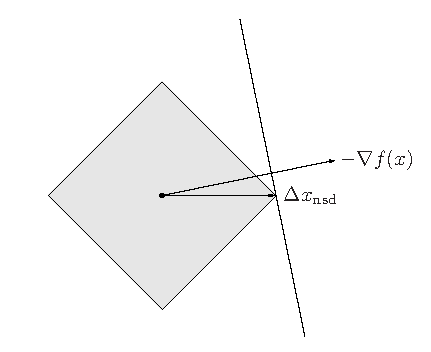
\includegraphics[width=.55\linewidth]{figures/ch09-fig10.pdf}
\caption*{图9.10\quad $\ell_1$ 范数的归一化最速下降方向。菱形为平移到 $x$ 的 $\ell_1$ 范数单位球。归一化最速下降方向总能取为某个标准基向量方向；本例中为 $\Delta x_{\mathrm{nsd}}=e_1$。}
\end{figure}
任取满足 $\norm{\nabla f(x)}_\infty=|(\nabla f(x))_i|$ 的指标 $i$，则一个 $\ell_1$ 范数归一化最速下降方向为
\[
\Delta x_{\mathrm{nsd}}
=-\operatorname{sign}\left(\frac{\partial f(x)}{\partial x_i}\right)e_i,
\]
其中 $e_i$ 是第 $i$ 个标准基向量。未归一化的最速下降步为
\[
\Delta x_{\mathrm{sd}}
=\Delta x_{\mathrm{nsd}}\norm{\nabla f(x)}_\infty
=-\frac{\partial f(x)}{\partial x_i}e_i.
\]
因此，$\ell_1$ 范数归一化最速下降步总可选为标准基向量或其相反数；它是使 $f$ 近似减小量最大的坐标轴方向，如图9.10所示。

$\ell_1$ 范数最速下降算法有很自然的解释：每次迭代选择 $\nabla f(x)$ 中绝对值最大的分量，再按 $(\nabla f(x))_i$ 的符号减小或增加 $x$ 的相应分量。由于每次迭代只更新 $x$ 的一个分量，它有时称为\emph{坐标下降算法}。这能大大简化线搜索，甚至使其变得极简单。

\begin{origexample}{9.2}
\emph{Frobenius范数缩放。}§4.5.4中遇到无约束几何规划
\[
\text{最小化}\quad\sum_{i,j=1}^n M_{ij}^2d_i^2/d_j^2,
\]
其中给定 $M\in\R^{n\times n}$，变量为 $d\in\R^n$。用变量替换 $x_i=2\log d_i$，可写为凸形式
\[
\text{最小化}\quad
f(x)=\log\left(\sum_{i,j=1}^n M_{ij}^2e^{x_i-x_j}\right).
\]

% Source PDF page 493 (printed p. 479)
每次仅对一个分量最小化 $f$ 很容易。保持除第 $k$ 个分量以外的所有分量不变，可写
$f(x)=\log(\alpha_k+\beta_ke^{-x_k}+\gamma_ke^{x_k})$，其中
\[
\alpha_k=M_{kk}^2+\sum_{i,j\ne k}M_{ij}^2e^{x_i-x_j},\quad
\beta_k=\sum_{i\ne k}M_{ik}^2e^{x_i},\quad
\gamma_k=\sum_{j\ne k}M_{kj}^2e^{-x_j}.
\]
$f(x)$ 作为 $x_k$ 的函数，在 $x_k=\log(\beta_k/\gamma_k)/2$ 处最小。因此，本例精确线搜索可用简单解析公式完成。

精确线搜索的 $\ell_1$ 最速下降算法重复以下步骤。
\begin{enumerate}
\item 计算梯度
\[
(\nabla f(x))_i=
\frac{-\beta_ie^{-x_i}+\gamma_ie^{x_i}}
{\alpha_i+\beta_ie^{-x_i}+\gamma_ie^{x_i}},\quad i=1,\ldots,n.
\]
\item 选择 $\nabla f(x)$ 的一个绝对值最大的分量：
$|\nabla f(x)|_k=\norm{\nabla f(x)}_\infty$。
\item 令 $x_k=\log(\beta_k/\gamma_k)/2$，在标量变量 $x_k$ 上最小化 $f$。
\end{enumerate}
\end{origexample}

\subsection{收敛分析}
本节将回溯线搜索梯度法的收敛分析推广到任意范数的最速下降法。利用任意范数可用欧几里得范数求界这一事实，即存在常数 $\gamma,\widetilde\gamma\in(0,1]$，满足
\[
\norm x\ge\gamma\norm x_2,\qquad
\norm x_*\ge\widetilde\gamma\norm x_2
\]
（见§A.1.4）。

仍假设 $f$ 在初始下水平集 $S$ 上强凸。上界 $\nabla^2f(x)\preceq MI$ 给出函数 $f(x+t\Delta x_{\mathrm{sd}})$ 关于 $t$ 的上界：
\begin{align}
f(x+t\Delta x_{\mathrm{sd}})
&\le f(x)+t\nabla f(x)^\T\Delta x_{\mathrm{sd}}
+\frac{M\norm{\Delta x_{\mathrm{sd}}}_2^2}{2}t^2\notag\\
&\le f(x)+t\nabla f(x)^\T\Delta x_{\mathrm{sd}}
+\frac{M\norm{\Delta x_{\mathrm{sd}}}^2}{2\gamma^2}t^2\notag\\
&=f(x)-t\norm{\nabla f(x)}_*^2
+\frac{M}{2\gamma^2}t^2\norm{\nabla f(x)}_*^2.\tag{9.26}
\end{align}
使二次上界（9.26）最小的步长 $\widehat t=\gamma^2/M$ 满足回溯线搜索退出条件：
\begin{equation}
\begin{split}
f(x+\widehat t\Delta x_{\mathrm{sd}})
&\le f(x)-\frac{\gamma^2}{2M}\norm{\nabla f(x)}_*^2\\
&\le f(x)+\frac{\alpha\gamma^2}{M}\nabla f(x)^\T\Delta x_{\mathrm{sd}},
\end{split}\tag{9.27}
\end{equation}

% Source PDF page 494 (printed p. 480)
因为 $\alpha<1/2$ 且 $\nabla f(x)^\T\Delta x_{\mathrm{sd}}=-\norm{\nabla f(x)}_*^2$。因此，线搜索返回步长 $t\ge\min\{1,\beta\gamma^2/M\}$，从而
\[
\begin{aligned}
f(x^+)=f(x+t\Delta x_{\mathrm{sd}})
&\le f(x)-\alpha\min\{1,\beta\gamma^2/M\}\norm{\nabla f(x)}_*^2\\
&\le f(x)-\alpha\widetilde\gamma^2\min\{1,\beta\gamma^2/M\}
\norm{\nabla f(x)}_2^2.
\end{aligned}
\]
两边减 $p^\star$，再用（9.9），得到
\[
f(x^+)-p^\star\le c(f(x)-p^\star),
\]
其中
\[
c=1-2m\alpha\widetilde\gamma^2\min\{1,\beta\gamma^2/M\}<1.
\]
因此
\[
f(x^{(k)})-p^\star\le c^k(f(x^{(0)})-p^\star),
\]
即与梯度法一样线性收敛。

\subsection{讨论与例子}
\subsubsection*{最速下降范数的选择}
定义最速下降方向所用范数的选择，可能极大影响收敛速率。为简便，考虑二次 $P$ 范数。§9.4.1已说明，它的最速下降法等同于在坐标变换 $\overline x=P^{1/2}x$ 后对问题应用梯度法。梯度法在下水平集（或最优点附近Hessian）条件数适中时效果好，条件数大时效果差。因此，坐标变换后下水平集条件适中，最速下降法就效果好。

这给出选择 $P$ 的原则：使经 $P^{-1/2}$ 变换后的 $f$ 下水平集条件良好。例如，若知道最优点处Hessian $H(x^\star)$ 的近似 $\widehat H$，一个很好的选择是 $P=\widehat H$，因为此时 $\widetilde f$ 在最优点处的Hessian为
\[
\widehat H^{-1/2}\nabla^2f(x^\star)\widehat H^{-1/2}\approx I,
\]
因而很可能有小条件数。

同一思想也可不用坐标变换表述。说下水平集经过 $\overline x=P^{1/2}x$ 变换后条件数小，等价于说椭球
\[
\mathcal E=\{x\mid x^\T Px\le1\}
\]
近似下水平集的形状。（即适当缩放和平移后，可很好地近似。）

收敛速率对 $P$ 选择的这种依赖，可从两面看。乐观的观点是，对于任意问题，总存在某种 $P$ 的选择，使最速下降法非常有效。

% Source PDF page 495 (printed p. 481)
\begin{figure}[htbp]\centering
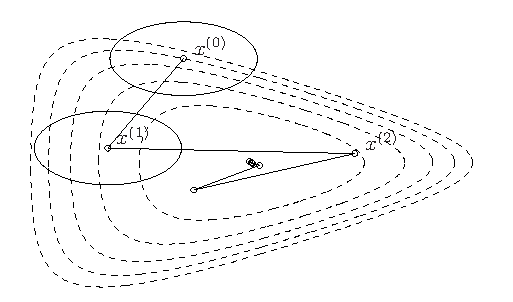
\includegraphics[width=.65\linewidth]{figures/ch09-fig11.pdf}
\caption*{图9.11\quad 采用二次范数 $\norm{\cdot}_{P_1}$ 的最速下降法。椭圆为 $x^{(0)}$ 和 $x^{(1)}$ 处范数球 $\{x\mid\norm{x-x^{(k)}}_{P_1}\le1\}$ 的边界。}
\end{figure}
难点当然是找到这样的 $P$。悲观的观点则是，对于任意问题，有大量 $P$ 的选择使最速下降法效果很差。总之，在能识别某个矩阵 $P$、使变换后问题的条件数适中的情况下，最速下降法效果好。

\subsubsection*{例子}
用目标为（9.20）的 $\R^2$ 非二次问题说明上述思想。采用两个二次范数的最速下降法，范数由
\[
P_1=\begin{bmatrix}2&0\\0&8\end{bmatrix},\qquad
P_2=\begin{bmatrix}8&0\\0&2\end{bmatrix}
\]
定义。两者都使用 $\alpha=0.1,\beta=0.7$ 的回溯线搜索。

图9.11、9.12显示 $\norm{\cdot}_{P_1}$ 和 $\norm{\cdot}_{P_2}$ 最速下降法的迭代点，图9.13显示两者误差随迭代次数的变化。范数选择强烈影响收敛：$\norm{\cdot}_{P_1}$ 比梯度法稍快，$\norm{\cdot}_{P_2}$ 则慢得多。

可通过分别经过 $\overline x=P_1^{1/2}x$ 和 $\overline x=P_2^{1/2}x$ 变换后的问题解释。图9.14、9.15显示变换坐标后的问题。$P_1$ 对应的变量替换得到条件数适中的下水平集，因而收敛快；$P_2$ 对应替换使下水平集条件更差，因而收敛较慢。

% Source PDF page 496 (printed p. 482)
\begin{figure}[htbp]\centering
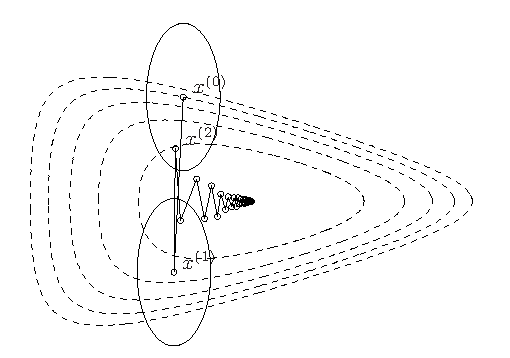
\includegraphics[width=.65\linewidth]{figures/ch09-fig12.pdf}
\caption*{图9.12\quad 采用二次范数 $\norm{\cdot}_{P_2}$ 的最速下降法。}
\end{figure}
\begin{figure}[htbp]\centering
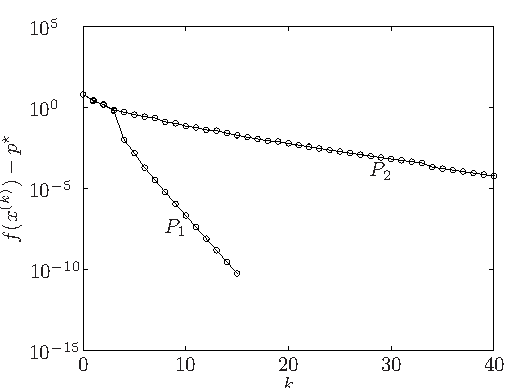
\includegraphics[width=.65\linewidth]{figures/ch09-fig13.pdf}
\caption*{图9.13\quad 采用二次范数 $\norm{\cdot}_{P_1}$ 和 $\norm{\cdot}_{P_2}$ 的最速下降法误差 $f(x^{(k)})-p^\star$ 随迭代次数 $k$ 的变化。$\norm{\cdot}_{P_1}$ 收敛快，$\norm{\cdot}_{P_2}$ 收敛很慢。}
\end{figure}

% Source PDF page 497 (printed p. 483)
\begin{figure}[htbp]\centering
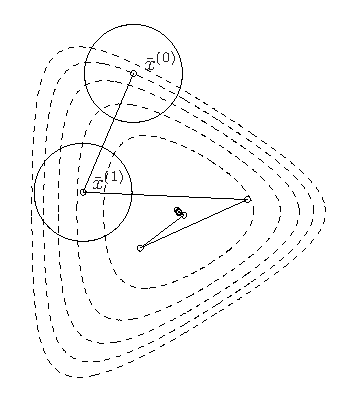
\includegraphics[width=.5\linewidth]{figures/ch09-fig14.pdf}
\caption*{图9.14\quad 坐标变换后，范数 $\norm{\cdot}_{P_1}$ 最速下降法的迭代点。这一变换减小下水平集条件数，从而加快收敛。}
\end{figure}
\begin{figure}[htbp]\centering
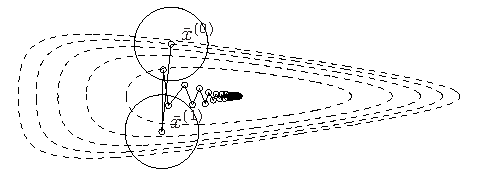
\includegraphics[width=.65\linewidth]{figures/ch09-fig15.pdf}
\caption*{图9.15\quad 坐标变换后，范数 $\norm{\cdot}_{P_2}$ 最速下降法的迭代点。这一变换增大下水平集条件数，从而减慢收敛。}
\end{figure}

% Source PDF page 498 (printed p. 484)
\begin{figure}[htbp]\centering
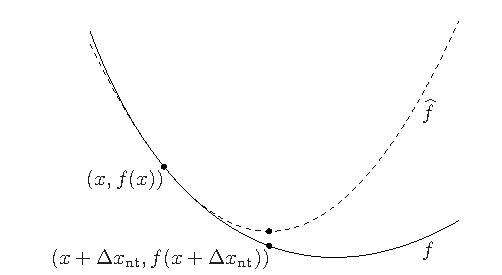
\includegraphics[width=.65\linewidth]{figures/ch09-fig16.pdf}
\caption*{图9.16\quad 函数 $f$（实线）与它在 $x$ 处的二阶近似 $\widehat f$（虚线）。将牛顿步 $\Delta x_{\mathrm{nt}}$ 加到 $x$ 上，就得到 $\widehat f$ 的最小点。}
\end{figure}
\section{牛顿法}
\subsection{牛顿步}
对 $x\in\dom f$，向量
\[
\Delta x_{\mathrm{nt}}=-\nabla^2f(x)^{-1}\nabla f(x)
\]
称为（$f$ 在 $x$ 处的）\emph{牛顿步}。$\nabla^2f(x)$ 的正定性意味着，除非 $\nabla f(x)=0$，否则
\[
\nabla f(x)^\T\Delta x_{\mathrm{nt}}
=-\nabla f(x)^\T\nabla^2f(x)^{-1}\nabla f(x)<0.
\]
因此牛顿步是下降方向（除非 $x$ 最优）。可以从几种角度解释并说明牛顿步。

\subsubsection*{二阶近似的最小点}
$f$ 在 $x$ 处的二阶Taylor近似（或模型）$\widehat f$ 为
\begin{equation}
\widehat f(x+v)=f(x)+\nabla f(x)^\T v+\tfrac12v^\T\nabla^2f(x)v.\tag{9.28}
\end{equation}
它是关于 $v$ 的凸二次函数，在 $v=\Delta x_{\mathrm{nt}}$ 时最小。因此，在 $x$ 上加牛顿步 $\Delta x_{\mathrm{nt}}$，就使 $f$ 在 $x$ 的二阶近似最小，如图9.16所示。

这个解释有助于理解牛顿步。若 $f$ 是二次函数，则 $x+\Delta x_{\mathrm{nt}}$ 就是精确最小点。若 $f$ 近似二次，直觉表明 $x+\Delta x_{\mathrm{nt}}$ 应很好地估计 $f$ 的最小点 $x^\star$。由于 $f$ 二阶可微，$x$ 靠近 $x^\star$ 时，其二次模型会很准确。因此 $x$ 靠近 $x^\star$ 时，$x+\Delta x_{\mathrm{nt}}$ 应很好地估计 $x^\star$。将会看到，这一直觉是正确的。

% Source PDF page 499 (printed p. 485)
\begin{figure}[htbp]\centering
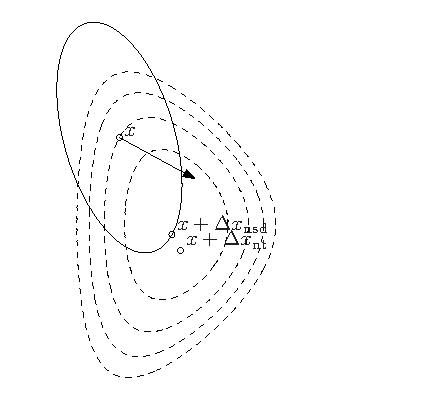
\includegraphics[width=.55\linewidth]{figures/ch09-fig17.pdf}
\caption*{图9.17\quad 虚线为凸函数的等值线，实线椭球为 $\{x+v\mid v^\T\nabla^2f(x)v\le1\}$。箭头表示梯度下降方向 $-\nabla f(x)$。牛顿步 $\Delta x_{\mathrm{nt}}$ 是范数 $\norm{\cdot}_{\nabla^2f(x)}$ 的最速下降方向；图中还表示该范数的归一化最速下降方向 $\Delta x_{\mathrm{nsd}}$。}
\end{figure}
\subsubsection*{Hessian范数下的最速下降方向}
牛顿步也是Hessian $\nabla^2f(x)$ 定义的二次范数
\[
\norm u_{\nabla^2f(x)}=(u^\T\nabla^2f(x)u)^{1/2}
\]
在 $x$ 处的最速下降方向。这再次说明为何牛顿步应是好的搜索方向，且 $x$ 靠近 $x^\star$ 时尤其好。

回顾上文讨论，若坐标变换后Hessian条件数小，二次范数 $\norm{\cdot}_P$ 最速下降法就收敛很快。特别地，在 $x^\star$ 附近，$P=\nabla^2f(x^\star)$ 是很好的选择。当 $x$ 靠近 $x^\star$，有 $\nabla^2f(x)\approx\nabla^2f(x^\star)$，由此解释牛顿步为何是极好的搜索方向，如图9.17所示。

\subsubsection*{线性化最优性条件的解}
在 $x$ 附近线性化最优性条件 $\nabla f(x^\star)=0$，得到
\[
\nabla f(x+v)\approx\nabla f(x)+\nabla^2f(x)v=0,
\]
这是关于 $v$ 的线性方程，解为 $v=\Delta x_{\mathrm{nt}}$。因此，在 $x$ 上加牛顿步就使线性化最优性条件成立。这同样表明，$x$ 靠近 $x^\star$（最优性条件已接近成立）时，更新 $x+\Delta x_{\mathrm{nt}}$ 应很好地近似 $x^\star$。

当 $n=1$，即 $f:\R\to\R$ 时，解释尤其简单。最小化问题的解 $x^\star$ 由 $f'(x^\star)=0$ 刻画，即导数 $f'$ 的过零点。

% Source PDF page 500 (printed p. 486)
\begin{figure}[htbp]\centering
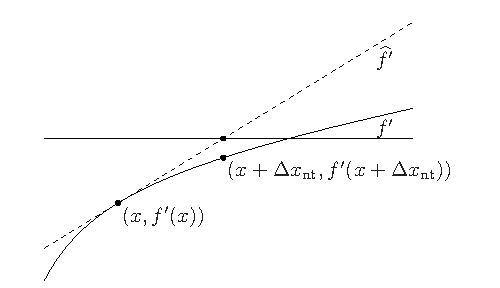
\includegraphics[width=.65\linewidth]{figures/ch09-fig18.pdf}
\caption*{图9.18\quad 实线为图9.16中 $f$ 的导数 $f'$。$\widehat f'$ 是 $f'$ 在 $x$ 处的线性近似。牛顿步 $\Delta x_{\mathrm{nt}}$ 是 $\widehat f'$ 的根与点 $x$ 的差。}
\end{figure}
由于 $f$ 凸，$f'$ 单调递增。给定当前解的近似 $x$，在 $x$ 处对 $f'$ 作一阶Taylor近似，这个仿射近似的过零点就是 $x+\Delta x_{\mathrm{nt}}$，如图9.18所示。

\subsubsection*{牛顿步的仿射不变性}
牛顿步的重要特点是独立于线性或仿射坐标变换。设 $T\in\R^{n\times n}$ 非奇异，定义 $\overline f(y)=f(Ty)$。有
\[
\nabla\overline f(y)=T^\T\nabla f(x),\qquad
\nabla^2\overline f(y)=T^\T\nabla^2f(x)T,
\]
其中 $x=Ty$。因此，$\overline f$ 在 $y$ 处的牛顿步为
\[
\begin{aligned}
\Delta y_{\mathrm{nt}}
&=-\bigl(T^\T\nabla^2f(x)T\bigr)^{-1}T^\T\nabla f(x)\\
&=-T^{-1}\nabla^2f(x)^{-1}\nabla f(x)\\
&=T^{-1}\Delta x_{\mathrm{nt}},
\end{aligned}
\]
其中 $\Delta x_{\mathrm{nt}}$ 是 $f$ 在 $x$ 处的牛顿步。因此 $f$ 和 $\overline f$ 的牛顿步由同一线性变换联系，并且
\[
x+\Delta x_{\mathrm{nt}}=T(y+\Delta y_{\mathrm{nt}}).
\]

\subsubsection*{牛顿减量}
量
\[
\lambda(x)=\bigl(\nabla f(x)^\T\nabla^2f(x)^{-1}\nabla f(x)\bigr)^{1/2}
\]
称为 $x$ 处的\emph{牛顿减量}。将会看到，它在牛顿法分析中起重要作用，也可用于

% Source PDF page 501 (printed p. 487)
停止准则。可以将牛顿减量与量 $f(x)-\inf_y\widehat f(y)$ 联系起来，其中 $\widehat f$ 为 $f$ 在 $x$ 的二阶近似：
\[
f(x)-\inf_y\widehat f(y)=f(x)-\widehat f(x+\Delta x_{\mathrm{nt}})
=\tfrac12\lambda(x)^2.
\]
因此，$\lambda^2/2$ 是基于 $f$ 在 $x$ 的二次近似，对 $f(x)-p^\star$ 作出的估计。

还可把牛顿减量写为
\begin{equation}
\lambda(x)=\bigl(\Delta x_{\mathrm{nt}}^\T\nabla^2f(x)\Delta x_{\mathrm{nt}}\bigr)^{1/2}.\tag{9.29}
\end{equation}
这说明 $\lambda$ 是Hessian定义的二次范数下牛顿步的范数，即范数
\[
\norm u_{\nabla^2f(x)}=(u^\T\nabla^2f(x)u)^{1/2}.
\]
牛顿减量也出现在回溯线搜索中，因为
\begin{equation}
\nabla f(x)^\T\Delta x_{\mathrm{nt}}=-\lambda(x)^2.\tag{9.30}
\end{equation}
它就是回溯线搜索使用的常数，并可解释为 $f$ 在 $x$ 处沿牛顿步的方向导数：
\[
-\lambda(x)^2=\nabla f(x)^\T\Delta x_{\mathrm{nt}}
=\left.\frac{\mathrm d}{\mathrm dt}f(x+\Delta x_{\mathrm{nt}}t)\right|_{t=0}.
\]

最后，牛顿减量与牛顿步一样具有仿射不变性。即当 $T$ 非奇异时，$\overline f(y)=f(Ty)$ 在 $y$ 的牛顿减量，与 $f$ 在 $x=Ty$ 的牛顿减量相同。

\subsection{牛顿法}
下面概述的牛顿法有时称为\emph{阻尼牛顿法}或\emph{保护牛顿法}，以区别于采用固定步长 $t=1$ 的\emph{纯牛顿法}。

\begin{origalgorithm}{9.5}
\emph{牛顿法。}

给定初始点 $x\in\dom f$，容差 $\epsilon>0$。

重复：
\begin{enumerate}
\item \emph{计算牛顿步与减量。}
\[
\Delta x_{\mathrm{nt}}:=-\nabla^2f(x)^{-1}\nabla f(x),\qquad
\lambda^2:=\nabla f(x)^\T\nabla^2f(x)^{-1}\nabla f(x).
\]
\item \emph{停止准则。}若 $\lambda^2/2\le\epsilon$，退出。
\item \emph{线搜索。}用回溯线搜索选择步长 $t$。
\item \emph{更新。}$x:=x+t\Delta x_{\mathrm{nt}}$。
\end{enumerate}
\end{origalgorithm}

它基本就是§9.2的一般下降方法，搜索方向取牛顿步。唯一差别很小：在计算搜索方向后检查停止准则，而非在更新后检查。

% Source PDF page 502 (printed p. 488)
\subsection{收敛分析}
仍假设 $f$ 二阶连续可微，且以常数 $m$ 强凸，即对 $x\in S$，$\nabla^2f(x)\succeq mI$。已知这还蕴含存在 $M>0$，使所有 $x\in S$ 满足 $\nabla^2f(x)\preceq MI$。

此外，假设 $f$ 的Hessian在 $S$ 上Lipschitz连续，常数为 $L$，即所有 $x,y\in S$ 满足
\begin{equation}
\norm{\nabla^2f(x)-\nabla^2f(y)}_2\le L\norm{x-y}_2.\tag{9.31}
\end{equation}
系数 $L$ 可理解为 $f$ 三阶导数的界；二次函数可取 $L=0$。更一般地，$L$ 衡量二次模型对 $f$ 的近似程度，因此可预期它对牛顿法性能起关键作用。直觉表明，若函数的二次模型变化缓慢（即 $L$ 小），牛顿法会非常有效。

\subsubsection*{收敛证明的思想与框架}
先给出证明的思想、框架和主要结论，再给出细节。将证明存在数 $\eta,\gamma$，其中 $0<\eta\le m^2/L$、$\gamma>0$，满足：
\begin{itemize}
\item 若 $\norm{\nabla f(x^{(k)})}_2\ge\eta$，则
\begin{equation}
f(x^{(k+1)})-f(x^{(k)})\le-\gamma.\tag{9.32}
\end{equation}
\item 若 $\norm{\nabla f(x^{(k)})}_2<\eta$，则回溯线搜索选择 $t^{(k)}=1$，且
\begin{equation}
\frac L{2m^2}\norm{\nabla f(x^{(k+1)})}_2
\le\left(\frac L{2m^2}\norm{\nabla f(x^{(k)})}_2\right)^2.\tag{9.33}
\end{equation}
\end{itemize}
分析第二个条件的含义。设它在第 $k$ 次迭代满足，即 $\norm{\nabla f(x^{(k)})}_2<\eta$。由于 $\eta\le m^2/L$，有 $\norm{\nabla f(x^{(k+1)})}_2<\eta$，所以第 $k+1$ 次也满足。递归下去，一旦第二个条件成立，所有后续迭代都成立，即对所有 $l\ge k$，$\norm{\nabla f(x^{(l)})}_2<\eta$。因此，对所有 $l\ge k$，算法都采用完整牛顿步 $t=1$，且
\begin{equation}
\frac L{2m^2}\norm{\nabla f(x^{(l+1)})}_2
\le\left(\frac L{2m^2}\norm{\nabla f(x^{(l)})}_2\right)^2.\tag{9.34}
\end{equation}
递归应用可知，对于 $l\ge k$，
\[
\frac L{2m^2}\norm{\nabla f(x^{(l)})}_2
\le\left(\frac L{2m^2}\norm{\nabla f(x^{(k)})}_2\right)^{2^{l-k}}
\le\left(\frac12\right)^{2^{l-k}},
\]
进而
\begin{equation}
f(x^{(l)})-p^\star\le\frac1{2m}\norm{\nabla f(x^{(l)})}_2^2
\le\frac{2m^3}{L^2}\left(\frac12\right)^{2^{l-k+1}}.\tag{9.35}
\end{equation}

% Source PDF page 503 (printed p. 489)
最后的不等式说明，一旦满足第二个条件，收敛就极快。这一现象称为\emph{二次收敛}。粗略地说，（9.35）意味着迭代足够多次后，每次迭代使正确数字位数加倍。

牛顿法迭代自然分为两个阶段。条件 $\norm{\nabla f(x)}_2\le\eta$ 成立后进入第二阶段，称为\emph{二次收敛阶段}。第一阶段称为\emph{阻尼牛顿阶段}，因为算法可能选择 $t<1$。二次收敛阶段也称\emph{纯牛顿阶段}，因为总选步长 $t=1$。

现在估计总复杂度。先为阻尼牛顿阶段迭代次数求上界。每次迭代 $f$ 至少减小 $\gamma$，所以阻尼牛顿步数不能超过
\[
\frac{f(x^{(0)})-p^\star}{\gamma};
\]
否则 $f$ 将小于 $p^\star$，这是不可能的。

用（9.35）为二次收敛阶段次数求界。它表明，经过不超过
\[
\log_2\log_2(\epsilon_0/\epsilon)
\]
次二次收敛阶段迭代，就必有 $f(x)-p^\star\le\epsilon$，其中 $\epsilon_0=2m^3/L^2$。

因此，达到 $f(x)-p^\star\le\epsilon$ 的总次数上界为
\begin{equation}
\frac{f(x^{(0)})-p^\star}{\gamma}
+\log_2\log_2(\epsilon_0/\epsilon).\tag{9.36}
\end{equation}
为二次收敛阶段次数求界的 $\log_2\log_2(\epsilon_0/\epsilon)$，随着精度要求提高而增长极慢，实际中可看作常数，例如五或六。（二次收敛阶段六次迭代得到约 $\epsilon\approx5\cdot10^{-20}\epsilon_0$ 的精度。）因此，略微不精确地说，最小化 $f$ 所需牛顿次数上界为
\begin{equation}
\frac{f(x^{(0)})-p^\star}{\gamma}+6.\tag{9.37}
\end{equation}
更准确地说，（9.37）为计算解的极好近似所需次数的界。

\subsubsection*{阻尼牛顿阶段}
下面证明（9.32）。假设 $\norm{\nabla f(x)}_2\ge\eta$。先为线搜索选取的步长求下界。强凸性蕴含 $S$ 上 $\nabla^2f(x)\preceq MI$，因此
\[
\begin{aligned}
f(x+t\Delta x_{\mathrm{nt}})
&\le f(x)+t\nabla f(x)^\T\Delta x_{\mathrm{nt}}
+\frac{M\norm{\Delta x_{\mathrm{nt}}}_2^2}{2}t^2\\
&\le f(x)-t\lambda(x)^2+\frac M{2m}t^2\lambda(x)^2,
\end{aligned}
\]

% Source PDF page 504 (printed p. 490)
这里利用（9.30）和
\[
\lambda(x)^2=\Delta x_{\mathrm{nt}}^\T\nabla^2f(x)\Delta x_{\mathrm{nt}}
\ge m\norm{\Delta x_{\mathrm{nt}}}_2^2.
\]
步长 $\widehat t=m/M$ 满足线搜索退出条件，因为
\[
f(x+\widehat t\Delta x_{\mathrm{nt}})
\le f(x)-\frac m{2M}\lambda(x)^2
\le f(x)-\alpha\widehat t\lambda(x)^2.
\]
因此线搜索返回 $t\ge\beta m/M$，使目标函数减小
\[
\begin{aligned}
f(x^+)-f(x)&\le-\alpha t\lambda(x)^2\\
&\le-\alpha\beta\frac mM\lambda(x)^2\\
&\le-\alpha\beta\frac m{M^2}\norm{\nabla f(x)}_2^2\\
&\le-\alpha\beta\eta^2\frac m{M^2},
\end{aligned}
\]
其中利用
\[
\lambda(x)^2=\nabla f(x)^\T\nabla^2f(x)^{-1}\nabla f(x)
\ge(1/M)\norm{\nabla f(x)}_2^2.
\]
因此取
\begin{equation}
\gamma=\alpha\beta\eta^2\frac m{M^2}\tag{9.38}
\end{equation}
即可满足（9.32）。

\subsubsection*{二次收敛阶段}
下面证明（9.33）。假设 $\norm{\nabla f(x)}_2<\eta$。先证明只要
\[
\eta\le3(1-2\alpha)\frac{m^2}{L},
\]
回溯线搜索就选择单位步长。

由Lipschitz条件（9.31），对 $t\ge0$，
\[
\norm{\nabla^2f(x+t\Delta x_{\mathrm{nt}})-\nabla^2f(x)}_2
\le tL\norm{\Delta x_{\mathrm{nt}}}_2,
\]
从而
\[
\left|\Delta x_{\mathrm{nt}}^\T
\bigl(\nabla^2f(x+t\Delta x_{\mathrm{nt}})-\nabla^2f(x)\bigr)
\Delta x_{\mathrm{nt}}\right|
\le tL\norm{\Delta x_{\mathrm{nt}}}_2^3.
\]
令 $\widetilde f(t)=f(x+t\Delta x_{\mathrm{nt}})$，则
$\widetilde f''(t)=\Delta x_{\mathrm{nt}}^\T\nabla^2f(x+t\Delta x_{\mathrm{nt}})\Delta x_{\mathrm{nt}}$，上式成为
\[
|\widetilde f''(t)-\widetilde f''(0)|
\le tL\norm{\Delta x_{\mathrm{nt}}}_2^3.
\]
用它为 $\widetilde f(t)$ 求上界。首先，
\[
\widetilde f''(t)\le\widetilde f''(0)+tL\norm{\Delta x_{\mathrm{nt}}}_2^3
\le\lambda(x)^2+t\frac L{m^{3/2}}\lambda(x)^3,
\]

% Source PDF page 505 (printed p. 491)
这里利用 $\widetilde f''(0)=\lambda(x)^2$ 和 $\lambda(x)^2\ge m\norm{\Delta x_{\mathrm{nt}}}_2^2$。积分得到
\[
\begin{aligned}
\widetilde f'(t)&\le\widetilde f'(0)+t\lambda(x)^2
+t^2\frac L{2m^{3/2}}\lambda(x)^3\\
&=-\lambda(x)^2+t\lambda(x)^2
+t^2\frac L{2m^{3/2}}\lambda(x)^3,
\end{aligned}
\]
其中利用 $\widetilde f'(0)=-\lambda(x)^2$。再积分一次，
\[
\widetilde f(t)\le\widetilde f(0)-t\lambda(x)^2
+\tfrac12t^2\lambda(x)^2+t^3\frac L{6m^{3/2}}\lambda(x)^3.
\]
最后取 $t=1$，得到
\begin{equation}
f(x+\Delta x_{\mathrm{nt}})
\le f(x)-\tfrac12\lambda(x)^2+\frac L{6m^{3/2}}\lambda(x)^3.\tag{9.39}
\end{equation}
设 $\norm{\nabla f(x)}_2\le\eta\le3(1-2\alpha)m^2/L$。由强凸性，
\[
\lambda(x)\le3(1-2\alpha)m^{3/2}/L.
\]
利用（9.39），有
\[
\begin{aligned}
f(x+\Delta x_{\mathrm{nt}})
&\le f(x)-\lambda(x)^2\left(\tfrac12-\frac{L\lambda(x)}{6m^{3/2}}\right)\\
&\le f(x)-\alpha\lambda(x)^2\\
&=f(x)+\alpha\nabla f(x)^\T\Delta x_{\mathrm{nt}},
\end{aligned}
\]
所以回溯线搜索接受单位步长 $t=1$。

再考察收敛速率。应用Lipschitz条件，
\[
\begin{aligned}
\norm{\nabla f(x^+)}_2
&=\norm{\nabla f(x+\Delta x_{\mathrm{nt}})-\nabla f(x)
-\nabla^2f(x)\Delta x_{\mathrm{nt}}}_2\\
&=\left\|\int_0^1
\bigl(\nabla^2f(x+t\Delta x_{\mathrm{nt}})-\nabla^2f(x)\bigr)
\Delta x_{\mathrm{nt}}\,\mathrm dt\right\|_2\\
&\le\frac L2\norm{\Delta x_{\mathrm{nt}}}_2^2\\
&=\frac L2\norm{\nabla^2f(x)^{-1}\nabla f(x)}_2^2\\
&\le\frac L{2m^2}\norm{\nabla f(x)}_2^2,
\end{aligned}
\]
即不等式（9.33）。

综上，若 $\norm{\nabla f(x^{(k)})}_2<\eta$，其中
\[
\eta=\min\{1,3(1-2\alpha)\}\frac{m^2}{L},
\]
则算法选取单位步长并满足（9.33）。将此界及（9.38）代入（9.37），得到迭代次数上界
\begin{equation}
6+\frac{M^2L^2/m^5}{\alpha\beta\min\{1,9(1-2\alpha)^2\}}
\bigl(f(x^{(0)})-p^\star\bigr).\tag{9.40}
\end{equation}

% Source PDF page 506 (printed p. 492)
\begin{figure}[htbp]\centering
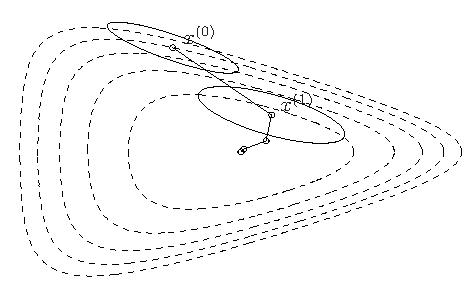
\includegraphics[width=.65\linewidth]{figures/ch09-fig19.pdf}
\caption*{图9.19\quad 对目标为（9.20）的 $\R^2$ 问题应用牛顿法，回溯参数为 $\alpha=0.1,\beta=0.7$。还显示前两个迭代点处的椭球 $\{x\mid\norm{x-x^{(k)}}_{\nabla^2f(x^{(k)})}\le1\}$。}
\end{figure}
\subsection{例子}
\subsubsection*{$\R^2$ 中的例子}
首先对测试函数（9.20）应用回溯线搜索牛顿法，参数 $\alpha=0.1,\beta=0.7$。图9.19显示牛顿迭代点，以及前两个迭代点 $k=0,1$ 的椭球
\[
\{x\mid\norm{x-x^{(k)}}_{\nabla^2f(x^{(k)})}\le1\}.
\]
方法有效，是因为这些椭球很好地近似下水平集的形状。

图9.20显示同一例子误差与迭代次数的关系，仅五次迭代就达到很高精度。二次收敛十分明显：最后一步把误差从约 $10^{-5}$ 降至 $10^{-10}$。

\subsubsection*{$\R^{100}$ 中的例子}
图9.21显示回溯与精确线搜索牛顿法在 $\R^{100}$ 问题上的收敛。目标具有（9.21）的形式，数据和初始点与图9.6相同。回溯线搜索曲线显示八次迭代即达很高精度。与 $\R^2$ 例子一样，第三次迭代后明显呈二次收敛。精确线搜索牛顿法仅比回溯少一次迭代，这也很典型：精确线搜索通常只对牛顿法收敛带来很小改进。图9.22显示步长。两个阻尼步之后，回溯线搜索所取均为完整步，即 $t=1$。

改变回溯参数 $\alpha,\beta$ 的实验表明，本例和其他例子中，它们对牛顿法性能影响很小。

% Source PDF page 507 (printed p. 493)
\begin{figure}[htbp]\centering
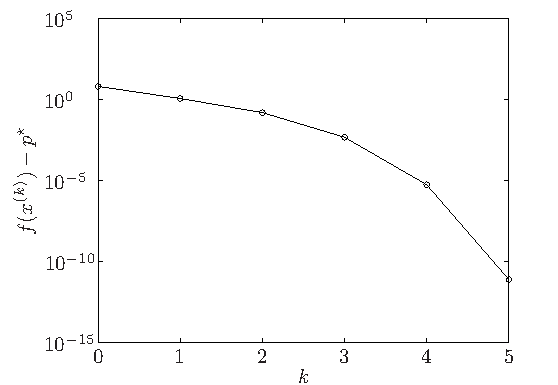
\includegraphics[width=.7\linewidth]{figures/ch09-fig20.pdf}
\caption*{图9.20\quad $\R^2$ 问题牛顿法的误差随迭代次数 $k$ 的变化。五次迭代即收敛到很高精度。}
\end{figure}
\begin{figure}[htbp]\centering
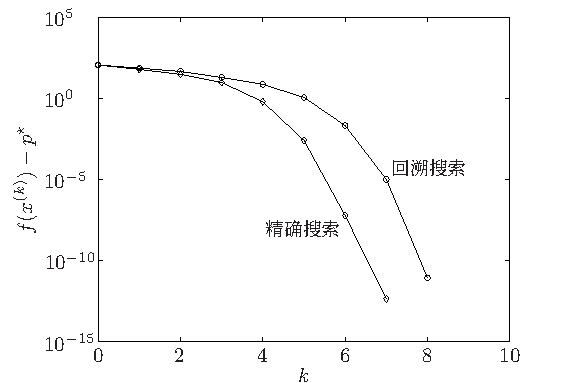
\includegraphics[width=.7\linewidth]{figures/ch09-fig21.pdf}
\caption*{图9.21\quad $\R^{100}$ 问题牛顿法的误差随迭代次数的变化。回溯参数为 $\alpha=0.01,\beta=0.5$。收敛也极快，七或八次迭代就有很高精度。精确线搜索仅比回溯快一次迭代。}
\end{figure}

% Source PDF page 508 (printed p. 494)
\begin{figure}[htbp]\centering
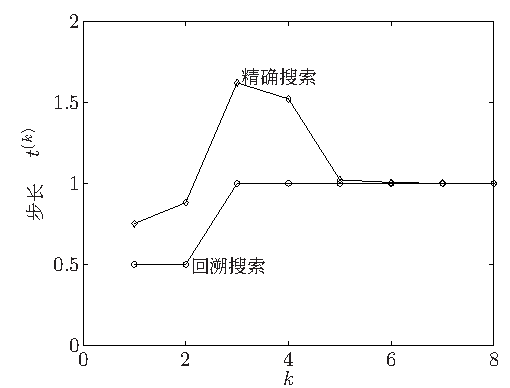
\includegraphics[width=.65\linewidth]{figures/ch09-fig22.pdf}
\caption*{图9.22\quad $\R^{100}$ 问题中，采用回溯和精确线搜索的牛顿法步长 $t$ 随迭代次数的变化。前两次迭代中，回溯线搜索各回溯一次；两次之后总选 $t=1$。}
\end{figure}
固定 $\alpha=0.01$，将 $\beta$ 在0.2至1之间变化，所需次数在8至12之间。固定 $\beta=0.5$，$\alpha$ 取0.005至0.5之间任意值时，所需次数均为8。因此多数实际实现采用较小 $\alpha$（如0.01）和较大 $\beta$（如0.5）的回溯线搜索。

\subsubsection*{$\R^{10000}$ 中的例子}
最后考虑一个更大的问题：
\[
\text{最小化}\quad
-\sum_{i=1}^n\log(1-x_i^2)-\sum_{i=1}^m\log(b_i-a_i^\T x),
\]
其中 $m=100000$、$n=10000$。数据 $a_i$ 是随机生成的稀疏向量。图9.23显示参数 $\alpha=0.01,\beta=0.5$ 的回溯线搜索牛顿法收敛。表现与前面的图很相似：约13次迭代的初始线性收敛阶段之后是二次收敛阶段，再用4或5次迭代就达很高精度。

\subsubsection*{牛顿法的仿射不变性}
牛顿法一个非常重要的特点是独立于线性或仿射坐标变换。设 $x^{(k)}$ 是对 $f:\R^n\to\R$ 应用牛顿法的第 $k$ 个迭代点。设 $T\in\R^{n\times n}$ 非奇异，定义 $\overline f(y)=f(Ty)$。若从 $y^{(0)}=T^{-1}x^{(0)}$ 出发，对 $\overline f$ 采用相同回溯参数的牛顿法，

% Source PDF page 509 (printed p. 495)
\begin{figure}[htbp]\centering
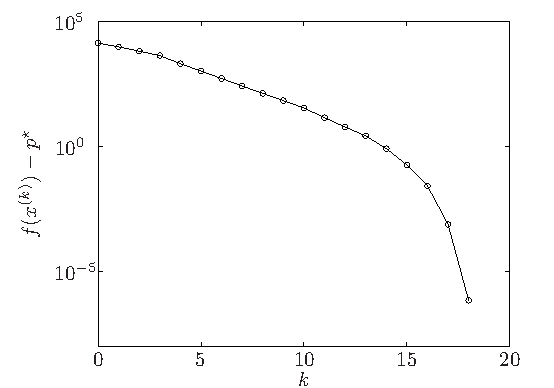
\includegraphics[width=.7\linewidth]{figures/ch09-fig23.pdf}
\caption*{图9.23\quad $\R^{10000}$ 问题的牛顿法误差随迭代次数的变化。采用 $\alpha=0.01,\beta=0.5$ 的回溯线搜索。即使这一大规模问题，牛顿法也仅需18次迭代就达很高精度。}
\end{figure}
则对所有 $k$，
\[
Ty^{(k)}=x^{(k)}.
\]
换言之，牛顿法相同：迭代点由同一个坐标变换联系。甚至停止准则也相同，因为 $\overline f$ 在 $y^{(k)}$ 的牛顿减量与 $f$ 在 $x^{(k)}$ 的相同。这与梯度法或最速下降法强烈受坐标变换影响形成鲜明对照。

例如，考虑（9.22）以参数 $\gamma$ 标记的问题族，$\gamma$ 影响下水平集条件数。图9.7和9.8中，当 $\gamma<0.05$ 或 $\gamma>20$，梯度法慢到无法使用。反之，对于 $10^{-10}$ 至 $10^{10}$ 间任意 $\gamma$，牛顿法（$\alpha=0.01,\beta=0.5$）都在九次迭代中求解此问题，而且精度高得多。

在采用有限精度运算的实际实现中，牛顿法并非完全独立于仿射坐标变换或下水平集条件数。不过，即使条件数高达 $10^{10}$，也不会对实际牛顿法实现造成不利影响；梯度法能容忍的条件数范围则小得多。坐标选择（或下水平集条件数）对梯度和最速下降法是首要问题，对牛顿法则是次要问题；它仅影响计算牛顿步所需的数值线性代数。

% Source PDF page 510 (printed p. 496)
\subsubsection*{小结}
牛顿法相比梯度与最速下降法，有几个突出的优点：
\begin{itemize}
\item 一般情况下收敛快，在 $x^\star$ 附近二次收敛。一旦进入二次收敛阶段，至多约六次迭代就能产生很高精度的解。
\item 仿射不变。对坐标选择或目标下水平集条件数不敏感。
\item 随问题规模增长表现良好。在 $\R^{10000}$ 问题上的表现与 $\R^{10}$ 相似，所需步数只适度增加。
\item 良好性能不依赖算法参数的选择。相比之下，最速下降法的范数选择对性能起关键作用。
\end{itemize}
牛顿法的主要缺点，是构造、存储Hessian以及计算牛顿步的成本；后者需要求解线性方程组。§9.7将说明，许多情况下可以利用问题结构，大幅降低牛顿步的计算成本。

另一选择是一类称为\emph{拟牛顿法}的无约束优化算法。它们形成搜索方向的计算量较小，但保留牛顿法的一些显著优点，例如在 $x^\star$ 附近快速收敛。由于许多书都介绍拟牛顿法，且它与本书主线关系不密切，本书不再讨论。

% Source PDF page 510 (printed p. 496), beginning of section 9.6.
\section{自协调}
第9.5.3节给出的牛顿法经典收敛性分析有两个主要不足。第一个是实际应用方面的：所得复杂度估计涉及三个常数 $m,M,L$，而在实际中，我们几乎从来不知道这些常数。因此，所需牛顿步数的界 (9.40) 几乎从来无法具体确定，因为它依赖于三个通常未知的常数。当然，收敛性分析与复杂度估计在概念上仍然有用。

第二个不足是，牛顿法本身具有仿射不变性，但经典分析却十分依赖所用坐标系。一旦改变坐标，常数 $m,M,L$ 就都会变化。即使仅仅出于形式上的考虑，我们也应该寻找一种像牛顿法本身一样、不依赖仿射坐标变换的分析。
% Source PDF page 511 (printed p. 497)
换句话说，我们希望找到一组条件，来代替假设
\[
 mI\preceq\nabla^2f(x)\preceq MI,\qquad
 \norm{\nabla^2f(x)-\nabla^2f(y)}_2\le L\norm{x-y}_2,
\]
使它们既不依赖仿射坐标变换，又能用于分析牛顿法。

Nesterov 和 Nemirovski 发现了一个简单而优美的假设，实现了这一目标，并将其称为\emph{自协调性}。自协调函数的重要性体现在几个方面。
\begin{itemize}
\item 求解凸优化问题的内点法中，许多起重要作用的对数障碍函数都是自协调函数。
\item 对自协调函数，牛顿法的分析不依赖任何未知常数。
\item 自协调性具有仿射不变性，即对自协调函数作变量的线性变换后，所得函数仍自协调。因此，牛顿法用于自协调函数时，所得复杂度估计不依赖仿射坐标变换。
\end{itemize}

\subsection{定义与例子}
\subsubsection*{$\R$ 上的自协调函数}
先考虑 $\R$ 上的函数。若凸函数 $f:\R\to\R$ 对所有 $x\in\dom f$ 满足
\begin{equation}
 \abs{f'''(x)}\le2f''(x)^{3/2},\tag{9.41}
\end{equation}
就称它\emph{自协调}。线性函数和凸二次函数的三阶导数为零，因此显然自协调。下面给出一些更有意思的例子。

\begin{origexample}{9.3}
\textbf{对数与熵。}
\begin{itemize}
\item \emph{负对数。}函数 $f(x)=-\log x$ 自协调。利用 $f''(x)=1/x^2$、$f'''(x)=-2/x^3$，得到
\[
 \frac{\abs{f'''(x)}}{2f''(x)^{3/2}}
 =\frac{2/x^3}{2(1/x^2)^{3/2}}=1,
\]
因此定义不等式 (9.41) 取等号。
\item \emph{负熵加负对数。}函数 $f(x)=x\log x-\log x$ 自协调。为验证这一点，利用
\[
 f''(x)=\frac{x+1}{x^2},\qquad f'''(x)=-\frac{x+2}{x^3},
\]
得到
\[
 \frac{\abs{f'''(x)}}{2f''(x)^{3/2}}
 =\frac{x+2}{2(x+1)^{3/2}}.
\]
% Source PDF page 512 (printed p. 498)
右端函数在 $\R_+$ 上于 $x=0$ 处取得最大值 $1$。

负熵函数本身并不自协调，见习题11.13。
\end{itemize}
\end{origexample}

关于自协调性的定义 (9.41)，有两点重要说明。第一点涉及定义中看似神秘的常数 $2$。选择这个常数其实是为了方便，使后面的公式更简单；也可以用其他任意正常数。比如，假设凸函数 $f:\R\to\R$ 满足
\begin{equation}
 \abs{f'''(x)}\le kf''(x)^{3/2},\tag{9.42}
\end{equation}
其中 $k$ 为某个正常数。那么函数 $\widetilde f(x)=(k^2/4)f(x)$ 满足
\[
\begin{aligned}
 \abs{\widetilde f'''(x)}&=(k^2/4)\abs{f'''(x)}\\
 &\le(k^3/4)f''(x)^{3/2}\\
 &=(k^3/4)\bigl((4/k^2)\widetilde f''(x)\bigr)^{3/2}\\
 &=2\widetilde f''(x)^{3/2},
\end{aligned}
\]
所以自协调。这说明，对于某个正常数 $k$ 满足 (9.42) 的函数，可以通过缩放使它满足标准自协调不等式 (9.41)。因此，关键在于函数的三阶导数以二阶导数的 $3/2$ 次幂的某个倍数为界。适当缩放函数，就能把这个倍数变成常数 $2$。

第二点通过一个简单计算，说明自协调性为何如此重要：它具有仿射不变性。设 $\widetilde f(y)=f(ay+b)$，其中 $a\ne0$，则 $\widetilde f$ 自协调，当且仅当 $f$ 自协调。为证明这一点，将
\[
 \widetilde f''(y)=a^2f''(x),\qquad
 \widetilde f'''(y)=a^3f'''(x),
\]
其中 $x=ay+b$，代入 $\widetilde f$ 的自协调不等式 $\abs{\widetilde f'''(y)}\le2\widetilde f''(y)^{3/2}$，得到
\[
 \abs{a^3f'''(x)}\le2\bigl(a^2f''(x)\bigr)^{3/2}.
\]
两边除以 $a^3$ 后，即得到 $f$ 的自协调不等式。大致说来，自协调条件 (9.41) 以一种不依赖仿射坐标变换的方式，限制了函数的三阶导数。

\subsubsection*{$\R^n$ 上的自协调函数}
现在考虑 $n>1$ 时 $\R^n$ 上的函数。若函数 $f:\R^n\to\R$ 沿其定义域内每条直线都自协调，即对所有 $x\in\dom f$ 和所有 $v$，函数 $\widetilde f(t)=f(x+tv)$ 作为 $t$ 的函数都自协调，就称 $f$ 自协调。

% Source PDF page 513 (printed p. 499)
\subsection{自协调函数的运算规则}
\subsubsection*{缩放与求和}
自协调性在乘以大于一的因子时保持：若 $f$ 自协调、$a\ge1$，则 $af$ 自协调。加法也保持自协调性：若 $f_1,f_2$ 自协调，则 $f_1+f_2$ 自协调。为证明这一点，只需考虑函数 $f_1,f_2:\R\to\R$。有
\[
\begin{aligned}
 \abs{f_1'''(x)+f_2'''(x)}
 &\le\abs{f_1'''(x)}+\abs{f_2'''(x)}\\
 &\le2\bigl(f_1''(x)^{3/2}+f_2''(x)^{3/2}\bigr)\\
 &\le2\bigl(f_1''(x)+f_2''(x)\bigr)^{3/2}.
\end{aligned}
\]
最后一步用了对 $u,v\ge0$ 成立的不等式
\[
 (u^{3/2}+v^{3/2})^{2/3}\le u+v.
\]

\subsubsection*{与仿射函数复合}
若 $f:\R^n\to\R$ 自协调，且 $A\in\R^{n\times m}$、$b\in\R^n$，则 $f(Ax+b)$ 自协调。

\begin{origexample}{9.4}
\textbf{线性不等式的对数障碍。}函数
\[
 f(x)=-\sum_{i=1}^m\log(b_i-a_i^\T x),
\]
定义域为 $\dom f=\{x\mid a_i^\T x<b_i,\ i=1,\ldots,m\}$，自协调。每一项 $-\log(b_i-a_i^\T x)$ 都是 $-\log y$ 与仿射变换 $y=b_i-a_i^\T x$ 的复合，因此自协调。所以它们的和也自协调。
\end{origexample}

\begin{origexample}{9.5}
\textbf{行列式的对数。}函数 $f(X)=-\log\det X$ 在 $\dom f=\mathbf S_{++}^n$ 上自协调。为证明这一点，考虑函数 $\widetilde f(t)=f(X+tV)$，其中 $X\succ0$、$V\in\mathbf S^n$。它可以写成
\[
\begin{aligned}
 \widetilde f(t)&=-\log\det\bigl(X^{1/2}(I+tX^{-1/2}VX^{-1/2})X^{1/2}\bigr)\\
 &=-\log\det X-\log\det(I+tX^{-1/2}VX^{-1/2})\\
 &=-\log\det X-\sum_{i=1}^n\log(1+t\lambda_i),
\end{aligned}
\]
其中 $\lambda_i$ 为 $X^{-1/2}VX^{-1/2}$ 的特征值。每一项 $-\log(1+t\lambda_i)$ 都是 $t$ 的自协调函数，因此它们的和 $\widetilde f$ 自协调。由此可知 $f$ 自协调。
\end{origexample}

\begin{origexample}{9.6}
\textbf{凹二次函数的对数。}函数
\[
 f(x)=-\log(x^\T Px+q^\T x+r),
\]
% Source PDF page 514 (printed p. 500)
其中 $P\in-\mathbf S_+^n$，在
\[
 \dom f=\{x\mid x^\T Px+q^\T x+r>0\}
\]
上自协调。为证明这一点，只需考虑 $n=1$，因为将 $f$ 限制在直线上，就把一般情形归结为 $n=1$ 的情形。此时可将 $f$ 写成
\[
 f(x)=-\log(px^2+qx+r)=-\log\bigl(-p(x-a)(b-x)\bigr),
\]
其中 $\dom f=(a,b)$，即 $a,b$ 是 $px^2+qx+r$ 的根。由此得到
\[
 f(x)=-\log(-p)-\log(x-a)-\log(b-x),
\]
因而证明了自协调性。
\end{origexample}

\subsubsection*{与对数复合}
设 $g:\R\to\R$ 为凸函数，$\dom g=\R_{++}$，且对所有 $x$ 有
\begin{equation}
 \abs{g'''(x)}\le3\frac{g''(x)}x.\tag{9.43}
\end{equation}
则函数
\[
 f(x)=-\log(-g(x))-\log x
\]
在 $\{x\mid x>0,\ g(x)<0\}$ 上自协调，证明见习题9.14。

条件 (9.43) 具有齐次性，并且在加法下保持。所有凸二次函数，即 $ax^2+bx+c$、$a\ge0$ 形式的函数，都满足该条件。因此，若函数 $g$ 满足 (9.43)，则函数 $g(x)+ax^2+bx+c$ 也满足，其中 $a\ge0$。

\begin{origexample}{9.7}
下列函数 $g$ 都满足条件 (9.43)。
\begin{itemize}
\item $g(x)=-x^p$，其中 $0<p\le1$。
\item $g(x)=-\log x$。
\item $g(x)=x\log x$。
\item $g(x)=x^p$，其中 $-1\le p\le0$。
\item $g(x)=(ax+b)^2/x$。
\end{itemize}
因此，每一种情形下，函数 $f(x)=-\log(-g(x))-\log x$ 都自协调。更一般地，只要 $a\ge0$，函数 $f(x)=-\log(-g(x)-ax^2-bx-c)-\log x$ 就在其定义域
\[
 \{x\mid x>0,\ g(x)+ax^2+bx+c<0\}
\]
上自协调。
\end{origexample}

\begin{origexample}{9.8}
与对数复合的规则，可用来证明下列函数自协调。
\begin{itemize}
\item $f(x,y)=-\log(y^2-x^\T x)$，定义在 $\{(x,y)\mid\norm x_2<y\}$ 上。
\item $f(x,y)=-2\log y-\log(y^{2/p}-x^2)$，其中 $p\ge1$，定义在 $\{(x,y)\in\R^2\mid\abs x^p<y\}$ 上。
\item $f(x,y)=-\log y-\log(\log y-x)$，定义在 $\{(x,y)\mid e^x<y\}$ 上。
\end{itemize}
细节留作习题9.15。
\end{origexample}

% Source PDF page 515 (printed p. 501)
\subsection{自协调函数的性质}
第9.1.2节利用强凸性，用点 $x$ 处的梯度范数导出了该点次优性的界。对于严格凸自协调函数，可以用牛顿减量得到类似的界：
\[
 \lambda(x)=\bigl(\nabla f(x)^\T\nabla^2f(x)^{-1}\nabla f(x)\bigr)^{1/2}.
\]
可以证明，严格凸自协调函数的 Hessian 处处正定，见习题9.17。与基于梯度范数的界不同，基于牛顿减量的界不受仿射坐标变换影响。

为供后面使用，注意牛顿减量还可以表示为
\[
 \lambda(x)=\sup_{v\ne0}\frac{-v^\T\nabla f(x)}{(v^\T\nabla^2f(x)v)^{1/2}},
\]
见习题9.9。换句话说，对任意非零 $v$，有
\begin{equation}
 \frac{-v^\T\nabla f(x)}{(v^\T\nabla^2f(x)v)^{1/2}}\le\lambda(x),\tag{9.44}
\end{equation}
当 $v=\Delta x_{\mathrm{nt}}$ 时取等号。

\subsubsection*{二阶导数的上界与下界}
设 $f:\R\to\R$ 为严格凸自协调函数。自协调不等式 (9.41) 可以写为
\begin{equation}
 \abs{\frac d{dt}\bigl(f''(t)^{-1/2}\bigr)}\le1,\tag{9.45}
\end{equation}
对所有 $t\in\dom f$ 成立，见习题9.16。假设 $t\ge0$，且 $0$ 与 $t$ 之间的区间在 $\dom f$ 中，将 (9.45) 从 $0$ 到 $t$ 积分，得到
\[
 -t\le\int_0^t\frac d{d\tau}\bigl(f''(\tau)^{-1/2}\bigr)\,d\tau\le t,
\]
即 $-t\le f''(t)^{-1/2}-f''(0)^{-1/2}\le t$。由此得到 $f''(t)$ 的下界与上界：
\begin{equation}
 \frac{f''(0)}{(1+tf''(0)^{1/2})^2}\le f''(t)
 \le\frac{f''(0)}{(1-tf''(0)^{1/2})^2}.\tag{9.46}
\end{equation}
下界对所有非负 $t\in\dom f$ 成立；上界要求 $t\in\dom f$ 且 $0\le t<f''(0)^{-1/2}$。

\subsubsection*{次优性的界}
设 $f:\R^n\to\R$ 为严格凸自协调函数，$v$ 为下降方向，即满足 $v^\T\nabla f(x)<0$ 的任意方向，不一定是
% Source PDF page 516 (printed p. 502)
牛顿方向。定义 $\widetilde f:\R\to\R$ 为 $\widetilde f(t)=f(x+tv)$。由定义，$\widetilde f$ 自协调。

对 (9.46) 中的下界积分，得到 $\widetilde f'(t)$ 的下界：
\begin{equation}
 \widetilde f'(t)\ge\widetilde f'(0)+\widetilde f''(0)^{1/2}
 -\frac{\widetilde f''(0)^{1/2}}{1+t\widetilde f''(0)^{1/2}}.\tag{9.47}
\end{equation}
再次积分，得到 $\widetilde f(t)$ 的下界：
\begin{equation}
 \widetilde f(t)\ge\widetilde f(0)+t\widetilde f'(0)+t\widetilde f''(0)^{1/2}
 -\log(1+t\widetilde f''(0)^{1/2}).\tag{9.48}
\end{equation}
右端在
\[
 \bar t=\frac{-\widetilde f'(0)}{\widetilde f''(0)+\widetilde f''(0)^{1/2}\widetilde f'(0)}
\]
处取得最小值。在 $\bar t$ 处求值，得到 $\widetilde f$ 的下界：
\[
\begin{aligned}
 \inf_{t\ge0}\widetilde f(t)
 &\ge\widetilde f(0)+\bar t\widetilde f'(0)+\bar t\widetilde f''(0)^{1/2}
 -\log(1+\bar t\widetilde f''(0)^{1/2})\\
 &=\widetilde f(0)-\widetilde f'(0)\widetilde f''(0)^{-1/2}
 +\log(1+\widetilde f'(0)\widetilde f''(0)^{-1/2}).
\end{aligned}
\]
不等式 (9.44) 可以写成
\[
 \lambda(x)\ge-\widetilde f'(0)\widetilde f''(0)^{-1/2},
\]
当 $v=\Delta x_{\mathrm{nt}}$ 时取等号，因为
\[
 \widetilde f'(0)=v^\T\nabla f(x),\qquad
 \widetilde f''(0)=v^\T\nabla^2f(x)v.
\]
利用 $u+\log(1-u)$ 是 $u$ 的单调递减函数这一事实以及上述不等式，得到
\[
 \inf_{t\ge0}\widetilde f(t)\ge\widetilde f(0)+\lambda(x)+\log(1-\lambda(x)).
\]
这个不等式对任意下降方向 $v$ 成立。因此，只要 $\lambda(x)<1$，就有
\begin{equation}
 p^\star\ge f(x)+\lambda(x)+\log(1-\lambda(x)).\tag{9.49}
\end{equation}
图9.24画出了函数 $-(\lambda+\log(1-\lambda))$。当 $\lambda$ 很小时，它满足
\[
 -(\lambda+\log(1-\lambda))\approx\lambda^2/2,
\]
且在 $\lambda\le0.68$ 时满足界
\[
 -(\lambda+\log(1-\lambda))\le\lambda^2.
\]
因此，得到次优性的界
\begin{equation}
 p^\star\ge f(x)-\lambda(x)^2,\tag{9.50}
\end{equation}
它在 $\lambda(x)\le0.68$ 时成立。

回顾，$\lambda(x)^2/2$ 是根据 $x$ 处二次模型给出的 $f(x)-p^\star$ 的估计。不等式 (9.50) 表明，对于自协调函数，将这一估计加倍，就能得到一个可证明的界。特别地，它说明，对于自协调函数，可以使用停止准则
\[
 \lambda(x)^2\le\epsilon,
\]
其中 $\epsilon<0.68^2$，并保证终止时有 $f(x)-p^\star\le\epsilon$。

% Source PDF page 517 (printed p. 503)
\begin{figure}[htbp]\centering
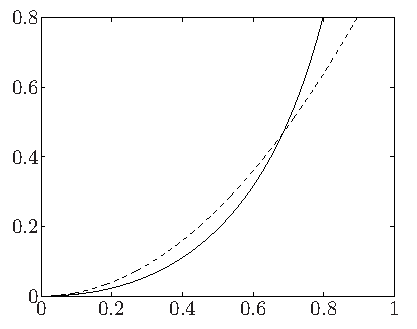
\includegraphics[width=.56\textwidth]{figures/ch09-later-24.pdf}
\caption*{图9.24 实线是函数 $-(\lambda+\log(1-\lambda))$，当 $\lambda$ 很小时，它近似为 $\lambda^2/2$。虚线为 $\lambda^2$，在区间 $0\le\lambda\le0.68$ 上是一个上界。}
\end{figure}
\subsection{自协调函数的牛顿法分析}
现在分析带回溯线搜索的牛顿法用于严格凸自协调函数 $f$ 时的情况。与前面一样，假设已知初始点 $x^{(0)}$，且下水平集 $S=\{x\mid f(x)\le f(x^{(0)})\}$ 闭。还假设 $f$ 有下界，这蕴含 $f$ 有最小点 $x^\star$，见习题9.19。

分析与第9.5.2节给出的经典分析十分相似，区别在于用自协调性代替强凸性与 Hessian 的 Lipschitz 条件作为基本假设，并且由牛顿减量代替梯度范数。我们将证明，存在仅依赖线搜索参数 $\alpha,\beta$ 的数 $\eta,\gamma>0$，且 $0<\eta\le1/4$，使以下结论成立。
\begin{itemize}
\item 若 $\lambda(x^{(k)})>\eta$，则
\begin{equation}
 f(x^{(k+1)})-f(x^{(k)})\le-\gamma.\tag{9.51}
\end{equation}
\item 若 $\lambda(x^{(k)})\le\eta$，则回溯线搜索选取 $t=1$，且
\begin{equation}
 2\lambda(x^{(k+1)})\le\bigl(2\lambda(x^{(k)})\bigr)^2.\tag{9.52}
\end{equation}
\end{itemize}
这些分别对应 (9.32) 和 (9.33)。与第9.5.3节一样，可递推应用第二个条件，得出对所有 $l\ge k$ 均有 $\lambda(x^{(l)})\le\eta$，且
\[
 2\lambda(x^{(l)})\le\bigl(2\lambda(x^{(k)})\bigr)^{2^{l-k}}
 \le(2\eta)^{2^{l-k}}\le\left(\frac12\right)^{2^{l-k}}.
\]
因此，对所有 $l\ge k$，
\[
 f(x^{(l)})-p^\star\le\lambda(x^{(l)})^2
 \le\frac14\left(\frac12\right)^{2^{l-k+1}}
 \le\left(\frac12\right)^{2^{l-k+1}},
\]
% Source PDF page 518 (printed p. 504)
所以，当 $l-k\ge\log_2\log_2(1/\epsilon)$ 时，有 $f(x^{(l)})-p^\star\le\epsilon$。

第一个不等式意味着，阻尼阶段所需步数不会超过 $(f(x^{(0)})-p^\star)/\gamma$。因此，从点 $x^{(0)}$ 出发，达到精度 $f(x)-p^\star\le\epsilon$ 所需的总迭代次数，以
\begin{equation}
 \frac{f(x^{(0)})-p^\star}{\gamma}+\log_2\log_2(1/\epsilon)\tag{9.53}
\end{equation}
为上界。这对应于牛顿法经典分析中的界 (9.36)。

\subsubsection*{阻尼牛顿阶段}
令 $\widetilde f(t)=f(x+t\Delta x_{\mathrm{nt}})$，则
\[
 \widetilde f'(0)=-\lambda(x)^2,\qquad
 \widetilde f''(0)=\lambda(x)^2.
\]
对 (9.46) 中的上界积分两次，得到 $\widetilde f(t)$ 的上界：
\begin{equation}
\begin{aligned}
 \widetilde f(t)&\le\widetilde f(0)+t\widetilde f'(0)-t\widetilde f''(0)^{1/2}
 -\log\bigl(1-t\widetilde f''(0)^{1/2}\bigr)\\
 &=\widetilde f(0)-t\lambda(x)^2-t\lambda(x)-\log(1-t\lambda(x)),
\end{aligned}\tag{9.54}
\end{equation}
在 $0\le t<1/\lambda(x)$ 时成立。

利用这个界，可以证明回溯线搜索总能给出步长 $t\ge\beta/(1+\lambda(x))$。为此，注意 $\hat t=1/(1+\lambda(x))$ 满足线搜索的退出条件：
\[
\begin{aligned}
 \widetilde f(\hat t)&\le\widetilde f(0)-\hat t\lambda(x)^2-\hat t\lambda(x)
 -\log(1-\hat t\lambda(x))\\
 &=\widetilde f(0)-\lambda(x)+\log(1+\lambda(x))\\
 &\le\widetilde f(0)-\alpha\frac{\lambda(x)^2}{1+\lambda(x)}\\
 &=\widetilde f(0)-\alpha\lambda(x)^2\hat t.
\end{aligned}
\]
第二个不等式来自对 $x\ge0$ 成立的事实
\[
 -x+\log(1+x)+\frac{x^2}{2(1+x)}\le0.
\]
由于 $t\ge\beta/(1+\lambda(x))$，有
\[
 \widetilde f(t)-\widetilde f(0)\le-\alpha\beta\frac{\lambda(x)^2}{1+\lambda(x)},
\]
因此 (9.51) 在
\[
 \gamma=\alpha\beta\frac{\eta^2}{1+\eta}
\]
时成立。

% Source PDF page 519 (printed p. 505)
\subsubsection*{二次收敛阶段}
我们将证明，可以取
\[
 \eta=(1-2\alpha)/4,
\]
它满足 $0<\eta<1/4$，因为 $0<\alpha<1/2$。也就是说，若 $\lambda(x^{(k)})\le(1-2\alpha)/4$，则回溯线搜索接受单位步长，并且 (9.52) 成立。

首先注意，上界 (9.54) 意味着，当 $\lambda(x)<1$ 时，单位步长 $t=1$ 得到的点位于 $\dom f$ 中。而且，若 $\lambda(x)\le(1-2\alpha)/2$，利用 (9.54)，有
\[
\begin{aligned}
 \widetilde f(1)&\le\widetilde f(0)-\lambda(x)^2-\lambda(x)-\log(1-\lambda(x))\\
 &\le\widetilde f(0)-\tfrac12\lambda(x)^2+\lambda(x)^3\\
 &\le\widetilde f(0)-\alpha\lambda(x)^2,
\end{aligned}
\]
因此单位步长满足充分下降条件。第二行来自：当 $0\le x\le0.81$ 时，$-x-\log(1-x)\le\tfrac12x^2+x^3$。

不等式 (9.52) 来自习题9.18中证明的下述事实：若 $\lambda(x)<1$，且 $x^+=x-\nabla^2f(x)^{-1}\nabla f(x)$，则
\begin{equation}
 \lambda(x^+)\le\frac{\lambda(x)^2}{(1-\lambda(x))^2}.\tag{9.55}
\end{equation}
特别地，若 $\lambda(x)\le1/4$，则
\[
 \lambda(x^+)\le2\lambda(x)^2,
\]
这就证明，当 $\lambda(x^{(k)})\le\eta$ 时，(9.52) 成立。

\subsubsection*{最终的复杂度界}
综合以上结果，牛顿迭代次数的界 (9.53) 成为
\begin{equation}
\begin{aligned}
 \frac{f(x^{(0)})-p^\star}{\gamma}+\log_2\log_2(1/\epsilon)
 ={}&\frac{20-8\alpha}{\alpha\beta(1-2\alpha)^2}
 \bigl(f(x^{(0)})-p^\star\bigr)\\
 &+\log_2\log_2(1/\epsilon).
\end{aligned}\tag{9.56}
\end{equation}
这一表达式只依赖线搜索参数 $\alpha,\beta$ 和最终精度 $\epsilon$。此外，涉及 $\epsilon$ 的项可以放心地用常数 $6$ 代替，因此这个界实际上只依赖 $\alpha,\beta$。对典型的 $\alpha,\beta$ 值，$f(x^{(0)})-p^\star$ 前面的系数大约为几百。例如，$\alpha=0.1$、$\beta=0.8$ 时，系数为 $375$。取容差 $\epsilon=10^{-10}$，得到界
\begin{equation}
 375\bigl(f(x^{(0)})-p^\star\bigr)+6.\tag{9.57}
\end{equation}
我们将看到，这个界相当保守，但它确实反映了所需牛顿步数的最坏值所呈现的一般形式。更精细的分析，例如 Nesterov 和 Nemirovski 最初给出的分析，可得到类似的界，但 $f(x^{(0)})-p^\star$ 前面的系数明显更小。

% Source PDF page 520 (printed p. 506)
\begin{figure}[htbp]\centering
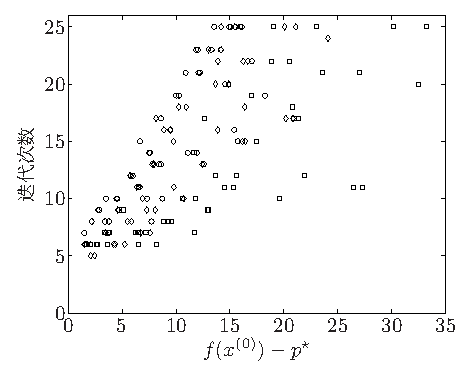
\includegraphics[width=.62\textwidth]{figures/ch09-later-25.pdf}
\caption*{图9.25 最小化自协调函数所需的牛顿迭代次数与 $f(x^{(0)})-p^\star$ 的关系。函数形式为 $f(x)=-\sum_{i=1}^m\log(b_i-a_i^\T x)$，问题数据 $a_i,b$ 随机生成。圆圈表示 $m=100,n=50$ 的问题，方框表示 $m=1000,n=500$ 的问题，菱形表示 $m=1000,n=50$ 的问题。每种问题各画出50个实例。}
\end{figure}
\subsection{讨论与数值例子}
\subsubsection*{一族自协调函数}
将上界 (9.57) 与最小化自协调函数实际所需的迭代次数进行比较，很有意思。考虑形如
\[
 f(x)=-\sum_{i=1}^m\log(b_i-a_i^\T x)
\]
的一族问题。

问题数据 $a_i,b$ 按以下方式生成。对每个问题实例，$a_i$ 的各分量由均值为零、方差为一的独立正态分布生成，$b$ 的各分量由 $[0,1]$ 上的均匀分布生成。剔除向下无界的问题实例。对每个问题，先计算 $x^\star$，再随机选择方向 $v$，取 $x^{(0)}=x^\star+sv$ 作为初始点，其中 $s$ 使 $f(x^{(0)})-p^\star$ 等于 $0$ 到 $35$ 之间的某个指定值。需要指出，$f(x^{(0)})-p^\star=10$ 或更大时，初始点实际上已经十分接近多面体边界。然后使用牛顿法最小化该函数，回溯线搜索参数取 $\alpha=0.1,\beta=0.8$，容差为 $\epsilon=10^{-10}$。

图9.25给出150个问题实例中，所需牛顿迭代次数与 $f(x^{(0)})-p^\star$ 的关系。圆圈表示 $m=100,n=50$ 的50个问题；方框表示 $m=1000,n=500$ 的50个问题；菱形表示 $m=1000,n=50$ 的50个问题。

% Source PDF page 521 (printed p. 507)
对这里所用的回溯参数，前面得到的复杂度界为
\begin{equation}
 375\bigl(f(x^{(0)})-p^\star\bigr)+6,\tag{9.58}
\end{equation}
显然远大于这150个实例实际所需的迭代次数。图中结果表明，可能存在一个形式相同的有效界，但 $f(x^{(0)})-p^\star$ 前面的常数小得多，例如约为 $1.5$。事实上，表达式
\[
 f(x^{(0)})-p^\star+6
\]
作为所需牛顿步数的粗略预测还不错，尽管它显然不是唯一因素。首先，有不少实例所需牛顿步数更少，可以猜测，它们对应比较“幸运”的初始点。还应注意，对于含500个变量的较大问题，即图中的方框，牛顿步数异常少的情形似乎更多。

这里需要说明，所研究的问题族不仅自协调，而且实际上是\emph{最小自协调}的，即当 $\alpha<1$ 时，$\alpha f$ 不自协调。因此，不能简单地缩放 $f$ 来改进界 (9.58)。函数 $f(x)=-20\log x$ 是自协调但并非最小自协调的例子，因为 $(1/20)f$ 也自协调。

\subsubsection*{自协调性在实际中的意义}
前面已经看到，对于强凸目标函数，牛顿法通常表现很好。这个概括性的说法可以通过经验结果支持，也可以通过牛顿法的经典分析来说明；经典分析给出了复杂度界，但它依赖几个几乎总是未知的常数。

对于自协调函数，我们能给出更明确的结论：复杂度界完全显式，不依赖任何未知常数。经验研究表明，这个界可以大幅收紧，但其一般形式，即一个小常数加上 $f(x^{(0)})-p^\star$ 的某个倍数，似乎至少能粗略预测最小化一个近似最小自协调函数所需的牛顿步数。

目前还不清楚，在实际中，牛顿法最小化自协调函数是否比最小化非自协调函数更容易；甚至还不清楚如何精确表述这一命题。目前能够说的是，与非自协调函数相比，自协调函数是一类能够对牛顿法复杂度作出更多明确论断的函数。

% Source PDF page 522 (printed p. 508)
\section{实现}
本节讨论实现无约束最小化算法时遇到的一些问题。数值线性代数的更多细节，见附录C。

\subsection{线搜索中的预计算}
在线搜索最简单的实现中，对每个 $t$ 求 $f(x+t\Delta x)$，与对任意 $z\in\dom f$ 求 $f(z)$ 的方式相同。但在某些情况下，可以利用需要沿射线 $\{x+t\Delta x\mid t\ge0\}$ 上许多点计算 $f$ 这一事实，在精确线搜索中还需计算其导数，来减少总计算量。这通常需要一些预计算，其代价往往与在任意一点计算 $f$ 的代价同阶；之后，沿该射线计算 $f$ 及其导数就可以更高效。

设 $x\in\dom f$、$\Delta x\in\R^n$，将 $f$ 限制在 $x$ 和 $\Delta x$ 确定的直线或射线上，定义 $\widetilde f(t)=f(x+t\Delta x)$。回溯线搜索需要对若干个、可能很多个 $t$ 值计算 $\widetilde f$；精确线搜索需要在若干 $t$ 值处计算 $\widetilde f$ 以及一阶或更高阶导数。上述简单方法先形成 $z=x+t\Delta x$，再求 $f(z)$，以计算 $\widetilde f(t)$。为计算 $\widetilde f'(t)$，先形成 $z=x+t\Delta x$，再求 $\nabla f(z)$，最后计算 $\widetilde f'(t)=\nabla f(z)^\T\Delta x$。下面用几个有代表性的例子，说明如何更高效地在多个 $t$ 值处计算 $\widetilde f$。

\subsubsection*{与仿射函数复合}
预计算能够加快线搜索的一种很一般的情形，是目标具有形式 $f(x)=\phi(Ax+b)$，其中 $A\in\R^{p\times n}$，$\phi$ 容易计算，例如是可分函数。用简单方法在 $k$ 个 $t$ 值处计算 $\widetilde f(t)=f(x+t\Delta x)$，需要对每个 $t$ 形成 $A(x+t\Delta x)+b$，共需 $2kpn$ 次浮点运算，然后对每个 $t$ 计算 $\phi(A(x+t\Delta x)+b)$。

更高效的方式是先计算 $Ax+b$ 和 $A\Delta x$，需要 $4pn$ 次浮点运算，再利用
\[
 A(x+t\Delta x)+b=(Ax+b)+t(A\Delta x)
\]
对每个 $t$ 形成 $A(x+t\Delta x)+b$，需要 $2kp$ 次浮点运算。只保留主导项，总代价为 $4pn+2kp$，而简单方法为 $2kpn$ 次浮点运算。

\subsubsection*{线性矩阵不等式的解析中心}
下面给出一个更具体、也更完整的例子。考虑计算线性矩阵不等式解析中心的问题 (9.6)，即最小化 $\log\det F(x)^{-1}$，其中 $x\in\R^n$，$F:\R^n\to\mathbf S^p$ 为仿射函数。沿着经过 $x$、方向为 $\Delta x$ 的直线，有
\[
 \widetilde f(t)=\log\det(F(x+t\Delta x))^{-1}=-\log\det(A+tB),
\]
% Source PDF page 523 (printed p. 509)
其中
\[
 A=F(x),\qquad B=\Delta x_1F_1+\cdots+\Delta x_nF_n\in\mathbf S^p.
\]
由于 $A\succ0$，它具有 Cholesky 分解 $A=LL^\T$，其中 $L$ 为非奇异下三角矩阵。因此，$\widetilde f$ 可以写成
\begin{equation}
\begin{aligned}
 \widetilde f(t)&=-\log\det\bigl(L(I+tL^{-1}BL^{-\T})L^\T\bigr)\\
 &=-\log\det A-\sum_{i=1}^p\log(1+t\lambda_i),
\end{aligned}\tag{9.59}
\end{equation}
其中 $\lambda_1,\ldots,\lambda_p$ 是 $L^{-1}BL^{-\T}$ 的特征值。一旦算出这些特征值，就能利用 (9.59) 右端的公式，对任意 $t$ 用 $4p$ 次简单算术运算求出 $\widetilde f(t)$。利用公式
\[
 \widetilde f'(t)=-\sum_{i=1}^p\frac{\lambda_i}{1+t\lambda_i},
\]
还可以用 $4p$ 次运算求出 $\widetilde f'(t)$，更高阶导数也类似。

假设线搜索需要在 $k$ 个 $t$ 值处求 $f(x+t\Delta x)$，比较这两种方法。简单方法对每个 $t$ 先形成 $F(x+t\Delta x)$，再以 $-\log\det F(x+t\Delta x)$ 计算 $f(x+t\Delta x)$。例如，可先求 Cholesky 分解 $F(x+t\Delta x)=LL^\T$，再计算
\[
 -\log\det F(x+t\Delta x)=-2\sum_{i=1}^p\log L_{ii}.
\]
形成 $F(x+t\Delta x)$ 的代价为 $np^2$，Cholesky 分解的代价为 $(1/3)p^3$，因此整个线搜索的总代价为
\[
 k\bigl(np^2+(1/3)p^3\bigr)=knp^2+(1/3)kp^3.
\]

使用前述方法，先形成 $A$，需要 $np^2$，再分解它，需要 $(1/3)p^3$。还要形成 $B$，需要 $np^2$，以及形成 $L^{-1}BL^{-\T}$，需要 $2p^3$。然后计算该矩阵的特征值，大约需要 $(4/3)p^3$ 次浮点运算。这些预计算总共需要 $2np^2+(11/3)p^3$ 次浮点运算。完成预计算后，对每个 $t$ 计算 $\widetilde f(t)$ 的代价为 $4p$ 次。因此，总代价为
\[
 2np^2+(11/3)p^3+4kp.
\]
若 $k$ 远小于 $p(2n+(11/3)p)$，这意味着整个线搜索的计算量，与仅计算一次 $f$ 相当。与简单方法相比，节省的计算量依赖于 $k,p,n$ 的取值，最高可达到 $k$ 倍的量级。

\subsection{计算牛顿步}
本节简要介绍实现牛顿法时遇到的一些问题。在多数情况下，计算牛顿步 $\Delta x_{\mathrm{nt}}$ 的工作量
% Source PDF page 524 (printed p. 510)
超过线搜索中的工作量。为计算牛顿步 $\Delta x_{\mathrm{nt}}$，先计算并形成 $x$ 处的 Hessian 矩阵 $H=\nabla^2f(x)$ 和梯度 $g=\nabla f(x)$，再求解线性方程组 $H\Delta x_{\mathrm{nt}}=-g$。这组方程有时称为\emph{牛顿方程组}，因为其解就是牛顿步；也称为\emph{正规方程组}，因为最小二乘问题的求解中也会出现同一类方程，见第9.1.1节。

虽然可以使用通用线性方程组求解器，但利用 $H$ 的对称性和正定性的方法更好。最常见的方法是形成 $H$ 的 Cholesky 分解，即计算满足 $LL^\T=H$ 的下三角矩阵 $L$，见第C.3.2节。然后通过前代求解 $Lw=-g$，得到 $w=-L^{-1}g$；再通过回代求解 $L^\T\Delta x_{\mathrm{nt}}=w$，得到
\[
 \Delta x_{\mathrm{nt}}=L^{-\T}w=-L^{-\T}L^{-1}g=-H^{-1}g.
\]
牛顿减量可以通过 $\lambda^2=-\Delta x_{\mathrm{nt}}^\T g$ 计算，也可以使用公式
\[
 \lambda^2=g^\T H^{-1}g=\norm{L^{-1}g}_2^2=\norm w_2^2.
\]
若使用稠密、无结构的 Cholesky 分解，前代与回代的代价被 Cholesky 分解的代价主导，后者为 $(1/3)n^3$ 次浮点运算。因此，计算牛顿步 $\Delta x_{\mathrm{nt}}$ 的总代价为 $F+(1/3)n^3$ 次浮点运算，其中 $F$ 是形成 $H,g$ 的代价。

通过利用 $H$ 的带状或稀疏等特殊结构，往往能更高效地求解牛顿方程组 $H\Delta x_{\mathrm{nt}}=-g$。这里“$H$ 的结构”指对所有 $x$ 都相同的结构。例如，说“$H$ 为三对角矩阵”，是指对每个 $x\in\dom f$，$\nabla^2f(x)$ 都为三对角矩阵。

\subsubsection*{带状结构}
若 Hessian $H$ 为带宽 $k$ 的带状矩阵，即当 $\abs{i-j}>k$ 时 $H_{ij}=0$，则可以使用带状 Cholesky 分解以及带状前代、回代。此时，计算牛顿步 $\Delta x_{\mathrm{nt}}=-H^{-1}g$ 的代价为 $F+nk^2$ 次浮点运算，假设 $k\ll n$；而稠密分解与代入方法需要 $F+(1/3)n^3$。

Hessian 的带状结构条件，即对所有 $x\in\dom f$ 有
\[
 \nabla^2f(x)_{ij}=\frac{\partial^2f(x)}{\partial x_i\partial x_j}=0
 \qquad\text{当 }\abs{i-j}>k,
\]
在目标函数 $f$ 中有一个有意思的解释。大致说来，在目标函数中，每个变量 $x_i$ 只与 $2k+1$ 个变量 $x_j$（$j=i-k,\ldots,i+k$）发生非线性耦合。当 $f$ 具有以下部分可分形式时，就会如此：
\[
 f(x)=\psi_1(x_1,\ldots,x_{k+1})+\psi_2(x_2,\ldots,x_{k+2})
 +\cdots+\psi_{n-k}(x_{n-k},\ldots,x_n),
\]
其中 $\psi_i:\R^{k+1}\to\R$。换句话说，$f$ 可以写成若干个分别依赖连续 $k$ 个变量的函数之和。

% Source PDF page 525 (printed p. 511)
\begin{origexample}{9.9}
考虑最小化 $f:\R^n\to\R$ 的问题，其中
\[
 f(x)=\psi_1(x_1,x_2)+\psi_2(x_2,x_3)+\cdots+\psi_{n-1}(x_{n-1},x_n),
\]
各 $\psi_i:\R^2\to\R$ 凸且二次可微。由于这种形式，Hessian $\nabla^2f$ 为三对角矩阵，因为 $\abs{i-j}>1$ 时，$\partial^2f/\partial x_i\partial x_j=0$。反过来，如果一个函数的 Hessian 对所有 $x$ 都是三对角矩阵，那么它就具有这种形式。

利用适用于三对角矩阵的 Cholesky 分解及前代、回代算法，求解这一问题的牛顿方程组只需要 $n$ 量级的浮点运算。若不利用 $f$ 的特殊形式，则需要 $n^3$ 量级的浮点运算。
\end{origexample}

\subsubsection*{稀疏结构}
更一般地，可以利用 Hessian $H$ 的稀疏性来求解牛顿方程组。当目标中的每个变量 $x_i$ 仅与少数其他变量非线性耦合时，就会出现这种稀疏结构；等价地，目标函数可以写成若干函数之和，其中每个函数仅依赖少数变量，而且每个变量仅出现在少数几个函数中。

当 $H$ 稀疏时，为求解 $H\Delta x=-g$，使用稀疏 Cholesky 分解，计算置换矩阵 $P$ 和下三角矩阵 $L$，使
\[
 H=PLL^\T P^\T.
\]
分解代价依赖具体的稀疏模式，但往往远小于 $(1/3)n^3$，在 $n$ 很大时，经验复杂度为 $n$ 量级的情形也并不少见。前代与回代与没有置换的基本方法很相似：通过前代求解 $Lw=-P^\T g$，再通过回代求解 $L^\T v=w$，得到
\[
 v=L^{-\T}w=-L^{-\T}L^{-1}P^\T g.
\]
牛顿步为 $\Delta x=Pv$。

由于 $H$ 的稀疏模式不随 $x$ 改变，更准确地说，由于我们只利用不随 $x$ 改变的稀疏性，因此每个牛顿步都可以使用同一个置换矩阵 $P$。确定一个好的置换矩阵 $P$ 的步骤称为\emph{符号分解步骤}，整个牛顿过程中只需进行一次。

\subsubsection*{对角加低秩}
求解牛顿方程组 $H\Delta x_{\mathrm{nt}}=-g$ 时，还可以利用许多其他类型的结构。这里只简要介绍一种，更多细节见附录C。假设 Hessian $H$ 可以表示为对角矩阵加一个低秩矩阵，其秩设为 $p$。当目标函数 $f$ 具有特殊形式
\begin{equation}
 f(x)=\sum_{i=1}^n\psi_i(x_i)+\psi_0(Ax+b)\tag{9.60}
\end{equation}
% Source PDF page 526 (printed p. 512)
时，就会如此，其中 $A\in\R^{p\times n}$，$\psi_1,\ldots,\psi_n:\R\to\R$，$\psi_0:\R^p\to\R$。换句话说，$f$ 是一个可分函数，加上一个仅依赖 $x$ 的低维仿射函数的函数。

为求出 (9.60) 的牛顿步 $\Delta x_{\mathrm{nt}}$，需要求解牛顿方程组 $H\Delta x_{\mathrm{nt}}=-g$，其中
\[
 H=D+A^\T H_0A.
\]
这里 $D=\diag(\psi_1''(x_1),\ldots,\psi_n''(x_n))$ 为对角矩阵，$H_0=\nabla^2\psi_0(Ax+b)$ 是 $\psi_0$ 的 Hessian。不利用这一结构计算牛顿步时，求解牛顿方程组的代价为 $(1/3)n^3$ 次浮点运算。

设 $H_0=L_0L_0^\T$ 是 $H_0$ 的 Cholesky 分解。引入临时变量 $w=L_0^\T A\Delta x_{\mathrm{nt}}\in\R^p$，将牛顿方程组写成
\[
 D\Delta x_{\mathrm{nt}}+A^\T L_0w=-g,\qquad
 w=L_0^\T A\Delta x_{\mathrm{nt}}.
\]
将由第一个方程得到的 $\Delta x_{\mathrm{nt}}=-D^{-1}(A^\T L_0w+g)$ 代入第二个方程，得到
\begin{equation}
 (I+L_0^\T AD^{-1}A^\T L_0)w=-L_0^\T AD^{-1}g,\tag{9.61}
\end{equation}
这是一个包含 $p$ 个线性方程的方程组。

现在按以下步骤计算牛顿步 $\Delta x_{\mathrm{nt}}$。先计算 $H_0$ 的 Cholesky 分解，代价为 $(1/3)p^3$；再形成 (9.61) 左端的稠密正定对称矩阵，代价为 $2p^2n$；然后通过 Cholesky 分解及回代、前代，求解 (9.61) 得到 $w$，代价为 $(1/3)p^3$ 次浮点运算。最后利用 $\Delta x_{\mathrm{nt}}=-D^{-1}(A^\T L_0w+g)$ 计算 $\Delta x_{\mathrm{nt}}$，代价为 $2np$ 次浮点运算。只保留主导项，计算 $\Delta x_{\mathrm{nt}}$ 的总代价为 $2p^2n$ 次浮点运算，当 $p\ll n$ 时，远小于 $(1/3)n^3$。

% Source PDF page 527 (printed p. 513)
\section*{文献说明}
\addcontentsline{toc}{section}{文献说明}
关于无约束最小化与非线性方程的算法，Dennis 和 Schnabel [DS96] 以及 Ortega 和 Rheinboldt [OR00] 是两部标准参考书。在强凸性与 Hessian 的 Lipschitz 连续性假设下得到的二次收敛结论，归于 Kantorovich [Kan52]。Polyak [Pol87，第1.6节] 对涉及未知常数的收敛结论的作用，给出了颇有见地的讨论，第9.5.3节导出的结论就属于这一类。

自协调函数由 Nesterov 和 Nemirovski [NN94] 引入。第9.6节和习题9.14至9.20中的全部结论，都可以在他们的书中找到，不过通常形式更一般，或者记号不同。Renegar [Ren01] 简明而优美地介绍了自协调函数，以及它们在原始—对偶内点算法分析中的作用。Peng、Roos 和 Terlaky [PRT02] 从自正则函数的角度研究内点法，这一类函数与自协调函数相似，但并不相同。

第9.7节相关内容的参考文献，见附录C末尾。

% Source PDF page 528 (printed p. 514)
\section*{习题}
\addcontentsline{toc}{section}{习题}
\subsection*{无约束最小化}
\paragraph{9.1} \emph{最小化二次函数。}考虑最小化二次函数的问题：
\[
 \text{最小化}\quad f(x)=\tfrac12x^\T Px+q^\T x+r,
\]
其中 $P\in\mathbf S^n$，但不假设 $P\succeq0$。
\begin{enumerate}[label=(\alph*)]
\item 证明，若 $P\not\succeq0$，即目标函数 $f$ 非凸，则问题向下无界。
\item 现在设 $P\succeq0$，因此目标函数凸，但最优性条件 $Px^\star=-q$ 无解。证明问题向下无界。
\end{enumerate}

\paragraph{9.2} \emph{最小化二次除以线性分式函数。}考虑最小化函数 $f:\R^n\to\R$ 的问题，其中
\[
 f(x)=\frac{\norm{Ax-b}_2^2}{c^\T x+d},\qquad
 \dom f=\{x\mid c^\T x+d>0\}.
\]
假设 $\rank A=n$ 且 $b\notin\mathcal R(A)$。
\begin{enumerate}[label=(\alph*)]
\item 证明 $f$ 为闭函数。
\item 证明，$f$ 的最小点 $x^\star$ 为
\[
 x^\star=x_1+tx_2,
\]
其中 $x_1=(A^\T A)^{-1}A^\T b$、$x_2=(A^\T A)^{-1}c$，$t\in\R$ 可以通过求解一个二次方程得到。
\end{enumerate}

\paragraph{9.3} \emph{初始点与下水平集条件。}考虑函数 $f(x)=x_1^2+x_2^2$，其定义域为 $\dom f=\{(x_1,x_2)\mid x_1>1\}$。
\begin{enumerate}[label=(\alph*)]
\item $p^\star$ 是多少？
\item 对 $x^{(0)}=(2,2)$，画出下水平集 $S=\{x\mid f(x)\le f(x^{(0)})\}$。$S$ 是否闭？$f$ 在 $S$ 上是否强凸？
\item 从 $x^{(0)}$ 出发，应用带回溯线搜索的梯度法，会发生什么？$f(x^{(k)})$ 是否收敛到 $p^\star$？
\end{enumerate}

\paragraph{9.4} 你是否同意以下论证？向量 $x\in\R^m$ 的 $\ell_1$ 范数可以表示为
\[
 \norm x_1=\frac12\inf_{y\succ0}\left(\sum_{i=1}^m x_i^2/y_i+\one^\T y\right).
\]
因此，$\ell_1$ 范数逼近问题
\[
 \text{最小化}\quad\norm{Ax-b}_1
\]
等价于最小化问题
\begin{equation}
 \text{最小化}\quad f(x,y)=\sum_{i=1}^m(a_i^\T x-b_i)^2/y_i+\one^\T y,\tag{9.62}
\end{equation}
其中 $\dom f=\{(x,y)\in\R^n\times\R^m\mid y\succ0\}$，$a_i^\T$ 是 $A$ 的第 $i$ 行。由于 $f$ 二次可微且凸，可以对 (9.62) 应用牛顿法，求解 $\ell_1$ 范数逼近问题。

\paragraph{9.5} \emph{回溯线搜索。}设 $f$ 强凸，满足 $mI\preceq\nabla^2f(x)\preceq MI$。设 $\Delta x$ 为 $x$ 处的下降方向。证明，在
\[
 0<t\le-\frac{\nabla f(x)^\T\Delta x}{M\norm{\Delta x}_2^2}
\]
时，回溯停止条件成立。利用这一结论，给出回溯迭代次数的上界。

% Source PDF page 529 (printed p. 515)
\subsection*{梯度法与最速下降法}
\paragraph{9.6} \emph{$\R^2$ 中的二次问题。}验证第9.3.2节第一个例子中迭代点 $x^{(k)}$ 的表达式。

\paragraph{9.7} 设 $\Delta x_{\mathrm{nsd}}$ 和 $\Delta x_{\mathrm{sd}}$ 分别为范数 $\norm{\cdot}$ 下 $x$ 处的归一化与未归一化最速下降方向。证明以下恒等式。
\begin{enumerate}[label=(\alph*)]
\item $\nabla f(x)^\T\Delta x_{\mathrm{nsd}}=-\norm{\nabla f(x)}_*$。
\item $\nabla f(x)^\T\Delta x_{\mathrm{sd}}=-\norm{\nabla f(x)}_*^2$。
\item $\Delta x_{\mathrm{sd}}=\argmin_v\bigl(\nabla f(x)^\T v+\tfrac12\norm v^2\bigr)$。
\end{enumerate}

\paragraph{9.8} \emph{$\ell_\infty$ 范数下的最速下降法。}说明如何找到 $\ell_\infty$ 范数下的最速下降方向，并给出简单解释。

\subsection*{牛顿法}
\paragraph{9.9} \emph{牛顿减量。}证明，牛顿减量 $\lambda(x)$ 满足
\[
 \lambda(x)=\sup_{v^\T\nabla^2f(x)v=1}\bigl(-v^\T\nabla f(x)\bigr)
 =\sup_{v\ne0}\frac{-v^\T\nabla f(x)}{(v^\T\nabla^2f(x)v)^{1/2}}.
\]

\paragraph{9.10} \emph{纯牛顿法。}若初始点不接近 $x^\star$，固定步长 $t=1$ 的牛顿法可能发散。本题考虑两个例子。
\begin{enumerate}[label=(\alph*)]
\item $f(x)=\log(e^x+e^{-x})$ 有唯一最小点 $x^\star=0$。分别从 $x^{(0)}=1$ 和 $x^{(0)}=1.1$ 出发，运行固定步长 $t=1$ 的牛顿法。
\item $f(x)=-\log x+x$ 有唯一最小点 $x^\star=1$。从 $x^{(0)}=3$ 出发，运行固定步长 $t=1$ 的牛顿法。
\end{enumerate}
画出 $f$ 和 $f'$，并标出前几个迭代点。

\paragraph{9.11} \emph{复合函数的梯度法与牛顿法。}设 $\phi:\R\to\R$ 递增且凸，$f:\R^n\to\R$ 凸，因此 $g(x)=\phi(f(x))$ 凸。假设 $f,g$ 二次可微。最小化 $f$ 与最小化 $g$ 两个问题显然等价。

比较对 $f,g$ 分别应用的梯度法和牛顿法。其搜索方向有何关系？若采用精确线搜索，这些方法之间有何关系？\emph{提示：}使用矩阵求逆引理，见第C.4.3节。

\paragraph{9.12} \emph{信赖域牛顿法。}若 $\nabla^2f(x)$ 奇异，或病态程度很高，则牛顿步
\[
 \Delta x_{\mathrm{nt}}=-\nabla^2f(x)^{-1}\nabla f(x)
\]
不能很好地定义。此时可以把搜索方向 $\Delta x_{\mathrm{tr}}$ 定义为下述问题的解：
\[
 \begin{aligned}\text{最小化}\quad&\tfrac12v^\T Hv+g^\T v\\
 \text{约束为}\quad&\norm v_2\le\gamma,
 \end{aligned}
\]
其中 $H=\nabla^2f(x)$、$g=\nabla f(x)$，$\gamma$ 为正常数。点 $x+\Delta x_{\mathrm{tr}}$ 在约束 $\norm{(x+\Delta x_{\mathrm{tr}})-x}_2\le\gamma$ 下，使 $f$ 在 $x$ 处的二阶近似最小。集合 $\{v\mid\norm v_2\le\gamma\}$ 称为\emph{信赖域}。参数 $\gamma$，即信赖域的大小，反映了我们对二阶模型的信心。

证明，对于某个 $\hat\beta$，$\Delta x_{\mathrm{tr}}$ 使
\[
 \tfrac12v^\T Hv+g^\T v+\hat\beta\norm v_2^2
\]
最小。这个二次函数可以解释为 $f$ 在 $x$ 附近的正则化二次模型。

% Source PDF page 530 (printed p. 516)
\subsection*{自协调性}
\paragraph{9.13} \emph{自协调性与倒数障碍。}
\begin{enumerate}[label=(\alph*)]
\item 证明，定义域为 $(0,8/9)$ 的函数 $f(x)=1/x$ 自协调。
\item 证明，函数
\[
 f(x)=\alpha\sum_{i=1}^m\frac1{b_i-a_i^\T x},
\]
定义域为 $\dom f=\{x\in\R^n\mid a_i^\T x<b_i,\ i=1,\ldots,m\}$，在 $\dom f$ 有界且
\[
 \alpha>(9/8)\max_{i=1,\ldots,m}\sup_{x\in\dom f}(b_i-a_i^\T x)
\]
时自协调。
\end{enumerate}

\paragraph{9.14} \emph{与对数复合。}设 $g:\R\to\R$ 为凸函数，$\dom g=\R_{++}$，并对所有 $x$ 满足
\[
 \abs{g'''(x)}\le3\frac{g''(x)}x.
\]
证明，$f(x)=-\log(-g(x))-\log x$ 在 $\{x\mid x>0,\ g(x)<0\}$ 上自协调。\emph{提示：}使用不等式
\[
 \frac32rp^2+q^3+\frac32p^2q+r^3\le1,
\]
它对满足 $p^2+q^2+r^2=1$ 的 $p,q,r\in\R_+$ 成立。

\paragraph{9.15} 证明下列函数自协调。证明时，将函数限制在直线上，并应用与对数复合的规则。
\begin{enumerate}[label=(\alph*)]
\item $f(x,y)=-\log(y^2-x^\T x)$，定义在 $\{(x,y)\mid\norm x_2<y\}$ 上。
\item $f(x,y)=-2\log y-\log(y^{2/p}-x^2)$，其中 $p\ge1$，定义在 $\{(x,y)\in\R^2\mid\abs x^p<y\}$ 上。
\item $f(x,y)=-\log y-\log(\log y-x)$，定义在 $\{(x,y)\mid e^x<y\}$ 上。
\end{enumerate}

\paragraph{9.16} 设 $f:\R\to\R$ 为自协调函数。
\begin{enumerate}[label=(\alph*)]
\item 假设 $f''(x)\ne0$。证明，自协调条件 (9.41) 可以表示为
\[
 \abs{\frac d{dx}\bigl(f''(x)^{-1/2}\bigr)}\le1.
\]
求一元“极端”自协调函数，即分别满足
\[
 \frac d{dx}\bigl(f''(x)^{-1/2}\bigr)=1,\qquad
 \frac d{dx}\bigl(\widetilde f''(x)^{-1/2}\bigr)=-1
\]
的函数 $f$ 与 $\widetilde f$。
\item 证明，或者对所有 $x\in\dom f$ 有 $f''(x)=0$，或者对所有 $x\in\dom f$ 有 $f''(x)>0$。
\end{enumerate}

\paragraph{9.17} \emph{自协调函数 Hessian 的上界与下界。}
\begin{enumerate}[label=(\alph*)]
\item 设 $f:\R^2\to\R$ 为自协调函数。证明，对所有 $x\in\dom f$，有
\[
 \abs{\frac{\partial^3f(x)}{\partial x_i^3}}
 \le2\left(\frac{\partial^2f(x)}{\partial x_i^2}\right)^{3/2},\qquad i=1,2,
\]
\[
 \abs{\frac{\partial^3f(x)}{\partial x_i^2\partial x_j}}
 \le2\frac{\partial^2f(x)}{\partial x_i^2}
 \left(\frac{\partial^2f(x)}{\partial x_j^2}\right)^{1/2},\qquad i\ne j.
\]
% Source PDF page 531 (printed p. 517)
\emph{提示：}若 $h:\R^2\times\R^2\times\R^2\to\R$ 为对称三线性型，即
\[
\begin{aligned}
 h(u,v,w)={}&a_1u_1v_1w_1+a_2(u_1v_1w_2+u_1v_2w_1+u_2v_1w_1)\\
 &+a_3(u_1v_2w_2+u_2v_1w_1+u_2v_2w_1)+a_4u_2v_2w_2,
\end{aligned}
\]
则
\[
 \sup_{u,v,w\ne0}\frac{h(u,v,w)}{\norm u_2\norm v_2\norm w_2}
 =\sup_{u\ne0}\frac{h(u,u,u)}{\norm u_2^3}.
\]
\item 设 $f:\R^n\to\R$ 为自协调函数。证明，$\nabla^2f(x)$ 的零空间与 $x$ 无关。证明，若 $f$ 严格凸，则对所有 $x\in\dom f$，$\nabla^2f(x)$ 非奇异。

\emph{提示：}证明，若对某个 $x\in\dom f$ 有 $w^\T\nabla^2f(x)w=0$，则对所有 $y\in\dom f$ 有 $w^\T\nabla^2f(y)w=0$。为此，将(a)的结论用于自协调函数 $\widetilde f(t,s)=f(x+t(y-x)+sw)$。
\item 设 $f:\R^n\to\R$ 为自协调函数，$x\in\dom f$、$v\in\R^n$。证明，当 $x+tv\in\dom f$、$0\le t<\alpha$ 时，有
\[
 (1-t\alpha)^2\nabla^2f(x)\preceq\nabla^2f(x+tv)
 \preceq\frac1{(1-t\alpha)^2}\nabla^2f(x),
\]
其中 $\alpha=(v^\T\nabla^2f(x)v)^{1/2}$。
\end{enumerate}

\paragraph{9.18} \emph{二次收敛。}设 $f:\R^n\to\R$ 为严格凸自协调函数，$\lambda(x)<1$，并定义 $x^+=x-\nabla^2f(x)^{-1}\nabla f(x)$。证明 $\lambda(x^+)\le\lambda(x)^2/(1-\lambda(x))^2$。\emph{提示：}使用习题9.17(c)中的不等式。

\paragraph{9.19} \emph{距最优点距离的界。}设 $f:\R^n\to\R$ 为严格凸自协调函数。
\begin{enumerate}[label=(\alph*)]
\item 假设 $\lambda(\bar x)<1$，且下水平集 $\{x\mid f(x)\le f(\bar x)\}$ 闭。证明，$f$ 的最小值可以取到，且
\[
 \bigl((\bar x-x^\star)^\T\nabla^2f(\bar x)(\bar x-x^\star)\bigr)^{1/2}
 \le\frac{\lambda(\bar x)}{1-\lambda(\bar x)}.
\]
\item 证明，若 $f$ 有一个闭下水平集，且 $f$ 有下界，则其最小值可以取到。
\end{enumerate}

\paragraph{9.20} \emph{自协调函数的共轭。}设 $f:\R^n\to\R$ 闭、严格凸且自协调。下面证明它的共轭，或 Legendre 变换 $f^*$，自协调。
\begin{enumerate}[label=(\alph*)]
\item 证明，对每个 $y\in\dom f^*$，都存在唯一的 $x\in\dom f$ 满足 $y=\nabla f(x)$。\emph{提示：}参阅习题9.19的结论。
\item 设 $\bar y=\nabla f(\bar x)$。定义
\[
 g(t)=f(\bar x+tv),\qquad h(t)=f^*(\bar y+tw),
\]
其中 $v\in\R^n$、$w=\nabla^2f(\bar x)v$。证明
\[
 g''(0)=h''(0),\qquad g'''(0)=-h'''(0).
\]
利用这些恒等式证明 $f^*$ 自协调。
\end{enumerate}

\paragraph{9.21} \emph{最优线搜索参数。}考虑最小化严格凸自协调函数所需牛顿迭代次数的上界 (9.56)。若对 $\alpha,\beta$ 求最小值，这个上界的最小值是多少？

\paragraph{9.22} 设 $f$ 严格凸，并满足 (9.42)。从 $x^{(0)}$ 出发，将 $p^\star$ 计算到精度 $\epsilon$ 所需的牛顿步数，有什么界？

% Source PDF page 532 (printed p. 518)
\subsection*{实现}
\paragraph{9.23} \emph{线搜索中的预计算。}对下列每个函数，说明如何通过预计算降低线搜索的计算代价。分别给出预计算的代价，以及使用和不使用预计算时，计算 $g(t)=f(x+t\Delta x)$ 与 $g'(t)$ 的代价。
\begin{enumerate}[label=(\alph*)]
\item $f(x)=-\sum_{i=1}^m\log(b_i-a_i^\T x)$。
\item $f(x)=\log\bigl(\sum_{i=1}^m\exp(a_i^\T x+b_i)\bigr)$。
\item $f(x)=(Ax-b)^\T(P_0+x_1P_1+\cdots+x_nP_n)^{-1}(Ax-b)$，其中 $P_i\in\mathbf S^m$、$A\in\R^{m\times n}$、$b\in\R^m$，且 $\dom f=\{x\mid P_0+\sum_{i=1}^n x_iP_i\succ0\}$。
\end{enumerate}

\paragraph{9.24} \emph{利用牛顿方程组的分块对角结构。}设凸函数 $f$ 的 Hessian $\nabla^2f(x)$ 为分块对角矩阵。计算牛顿步时，如何利用这一结构？它意味着 $f$ 具有什么性质？

\paragraph{9.25} \emph{给定数据的平滑拟合。}考虑问题
\[
 \text{最小化}\quad f(x)=\sum_{i=1}^n\psi(x_i-y_i)+\lambda\sum_{i=1}^{n-1}(x_{i+1}-x_i)^2,
\]
其中 $\lambda>0$ 为平滑参数，$\psi$ 为凸惩罚函数，$x\in\R^n$ 为变量。可以将 $x$ 解释为向量 $y$ 的平滑拟合。
\begin{enumerate}[label=(\alph*)]
\item $f$ 的 Hessian 具有什么结构？
\item 推广到二维数据的平滑拟合问题，即最小化函数
\[
\begin{aligned}
 &\sum_{i,j=1}^n\psi(x_{ij}-y_{ij})\\
 &\quad+\lambda\left(\sum_{i=1}^{n-1}\sum_{j=1}^n(x_{i+1,j}-x_{ij})^2
 +\sum_{i=1}^n\sum_{j=1}^{n-1}(x_{i,j+1}-x_{ij})^2\right),
\end{aligned}
\]
变量为 $X\in\R^{n\times n}$，给定数据为 $Y\in\R^{n\times n}$ 和 $\lambda>0$。
\end{enumerate}

\paragraph{9.26} \emph{具有线性结构的牛顿方程。}考虑最小化形如
\begin{equation}
 f(x)=\sum_{i=1}^N\psi_i(A_ix+b_i)\tag{9.63}
\end{equation}
的函数，其中 $A_i\in\R^{m_i\times n}$、$b_i\in\R^{m_i}$，各函数 $\psi_i:\R^{m_i}\to\R$ 二次可微且凸。$f$ 在 $x$ 处的 Hessian $H$ 与梯度 $g$ 为
\begin{equation}
 H=\sum_{i=1}^N A_i^\T H_iA_i,\qquad
 g=\sum_{i=1}^N A_i^\T g_i,\tag{9.64}
\end{equation}
其中 $H_i=\nabla^2\psi_i(A_ix+b_i)$、$g_i=\nabla\psi_i(A_ix+b_i)$。

说明你会怎样实现最小化 $f$ 的牛顿法。假设 $n\gg m_i$，各矩阵 $A_i$ 非常稀疏，但 Hessian $H$ 稠密。

\paragraph{9.27} \emph{带变量界的线性不等式解析中心。}给出计算下列函数牛顿步的最高效方法：
\[
 f(x)=-\sum_{i=1}^n\log(x_i+1)-\sum_{i=1}^n\log(1-x_i)
 -\sum_{i=1}^m\log(b_i-a_i^\T x),
\]
其中 $\dom f=\{x\in\R^n\mid-\one\prec x\prec\one,\ Ax\prec b\}$，$a_i^\T$ 是 $A$ 的第 $i$ 行。假设 $A$ 稠密，并区分 $m\ge n$ 与 $m\le n$ 两种情况，另见习题9.30。

% Source PDF page 533 (printed p. 519)
\paragraph{9.28} \emph{二次不等式的解析中心。}描述一种高效计算下列函数牛顿步的方法：
\[
 f(x)=-\sum_{i=1}^m\log(-x^\T A_ix-b_i^\T x-c_i),
\]
其中 $\dom f=\{x\mid x^\T A_ix+b_i^\T x+c_i<0,\ i=1,\ldots,m\}$。假设各矩阵 $A_i\in\mathbf S_{++}^n$ 规模很大且稀疏，并且 $m\ll n$。

\emph{提示：}$f$ 在 $x$ 处的 Hessian 与梯度为
\[
 H=\sum_{i=1}^m\bigl(2\alpha_iA_i+\alpha_i^2(2A_ix+b_i)(2A_ix+b_i)^\T\bigr),
 \qquad g=\sum_{i=1}^m\alpha_i(2A_ix+b_i),
\]
其中 $\alpha_i=1/(-x^\T A_ix-b_i^\T x-c_i)$。

\paragraph{9.29} \emph{利用两阶段优化的结构。}本题接续习题4.64，后者介绍了带补救的优化，即两阶段优化。采用习题4.64中的记号与假设，并进一步假设：对每个情景 $i=1,\ldots,S$，代价函数 $f$ 都是关于 $(x,z)$ 的二次可微函数。

说明如何高效计算寻找最优策略这一问题的牛顿步。作为情景数量 $S$ 的函数，你的方法与不利用任何结构的通用方法相比，近似 flop 数有何差别？

\subsection*{数值实验}
\paragraph{9.30} \emph{梯度法与牛顿法。}考虑无约束问题
\[
 \text{最小化}\quad f(x)=-\sum_{i=1}^m\log(1-a_i^\T x)-\sum_{i=1}^n\log(1-x_i^2),
\]
变量为 $x\in\R^n$，定义域为 $\dom f=\{x\mid a_i^\T x<1,\ i=1,\ldots,m,\ \abs{x_i}<1,\ i=1,\ldots,n\}$。这是计算线性不等式组
\[
 a_i^\T x\le1,\quad i=1,\ldots,m,\qquad
 \abs{x_i}\le1,\quad i=1,\ldots,n
\]
的解析中心问题。注意，可以选 $x^{(0)}=0$ 作为初始点。可以从 $\R^n$ 上的某个分布中抽取 $a_i$，来生成问题实例。
\begin{enumerate}[label=(\alph*)]
\item 使用梯度法求解，合理选择回溯参数，并使用 $\norm{\nabla f(x)}_2\le\eta$ 形式的停止准则。画出目标函数值与步长随迭代次数变化的曲线。在高精度确定 $p^\star$ 后，也可以画出 $f-p^\star$ 随迭代次数变化的曲线。尝试不同的回溯参数 $\alpha,\beta$，观察它们对所需总迭代次数的影响。对几个不同规模的问题实例进行实验。
\item 使用牛顿法重复实验，采用基于牛顿减量 $\lambda^2$ 的停止准则。观察是否出现二次收敛。无需像习题9.27那样高效计算牛顿步，可以使用通用稠密求解器，不过最好使用基于 Cholesky 分解的求解器。
\end{enumerate}
\emph{提示：}利用链式法则，求出 $\nabla f(x)$ 与 $\nabla^2f(x)$ 的表达式。

\paragraph{9.31} \emph{几种近似牛顿法。}牛顿法的代价主要由计算 Hessian $\nabla^2f(x)$ 与求解牛顿方程组的代价决定。对大规模问题，有时可以用一个正定近似替代 Hessian，使形成和求解搜索步更容易。本题研究这一思想的几个常见例子。

对下面每种近似牛顿法，在习题9.30的解析中心问题的若干实例上进行测试，并将结果与牛顿法、梯度法所得结果比较。
% Source PDF page 534 (printed p. 520)
\begin{enumerate}[label=(\alph*)]
\item \emph{复用 Hessian。}只在每隔 $N$ 次迭代时计算并分解 Hessian，其中 $N>1$，并使用搜索步 $\Delta x=-H^{-1}\nabla f(x)$，$H$ 为最近一次计算的 Hessian。每 $N$ 步只需计算并分解一次 Hessian；其他步骤通过回代与前代计算搜索方向。
\item \emph{对角近似。}用 Hessian 的对角部分代替它，因此只需计算 $n$ 个二阶导数 $\partial^2f(x)/\partial x_i^2$，搜索步也很容易计算。
\end{enumerate}

\paragraph{9.32} \emph{凸非线性最小二乘问题的 Gauss--Newton 法。}考虑非线性最小二乘问题，最小化形如
\[
 f(x)=\frac12\sum_{i=1}^m f_i(x)^2
\]
的函数，其中各 $f_i$ 二次可微。$f$ 在 $x$ 处的梯度与 Hessian 为
\[
 \nabla f(x)=\sum_{i=1}^m f_i(x)\nabla f_i(x),\qquad
 \nabla^2f(x)=\sum_{i=1}^m\bigl(\nabla f_i(x)\nabla f_i(x)^\T+f_i(x)\nabla^2f_i(x)\bigr).
\]
考虑 $f$ 凸的情形。例如，当每个 $f_i$ 或者非负且凸，或者非正且凹，或者为仿射函数时，就会如此。

Gauss--Newton 法采用搜索方向
\[
 \Delta x_{\mathrm{gn}}=-\left(\sum_{i=1}^m\nabla f_i(x)\nabla f_i(x)^\T\right)^{-1}
 \left(\sum_{i=1}^m f_i(x)\nabla f_i(x)\right).
\]
这里假设逆存在，即向量 $\nabla f_1(x),\ldots,\nabla f_m(x)$ 张成 $\R^n$。这个方向可以看作一种近似牛顿方向，见习题9.31：从 $f$ 的 Hessian 中去掉二阶导数项，就得到它。

Gauss--Newton 搜索方向 $\Delta x_{\mathrm{gn}}$ 还有另一个简单解释。利用一阶近似 $f_i(x+v)\approx f_i(x)+\nabla f_i(x)^\T v$，得到
\[
 f(x+v)\approx\frac12\sum_{i=1}^m\bigl(f_i(x)+\nabla f_i(x)^\T v\bigr)^2.
\]
Gauss--Newton 搜索步 $\Delta x_{\mathrm{gn}}$ 恰好是使 $f$ 的这个近似最小的 $v$。因此，还可得出 $\Delta x_{\mathrm{gn}}$ 可以通过求解线性最小二乘问题计算。

在形如下式的一些问题实例上测试 Gauss--Newton 法：
\[
 f_i(x)=\tfrac12x^\T A_ix+b_i^\T x+1,
\]
其中 $A_i\in\mathbf S_{++}^n$，且 $b_i^\T A_i^{-1}b_i\le2$，这一条件保证 $f$ 凸。



\chapter{等式约束最小化}
% Source PDF page 535 (printed p. 521)
\section{等式约束最小化问题}
本章介绍求解带等式约束的凸优化问题的方法：
\begin{equation}\begin{array}{ll}\text{最小化}&f(x)\\\text{约束条件}&Ax=b,\end{array}\tag{10.1}\end{equation}
其中 $f:\R^n\to\R$ 是凸函数，且二阶连续可微，$A\in\R^{p\times n}$，$\rank A=p<n$。关于 $A$ 的假设表示：等式约束的数量少于变量数，而且等式约束彼此独立。假设最优解 $x^\star$ 存在，并以 $p^\star$ 表示最优值，$p^\star=\inf\{f(x)\mid Ax=b\}=f(x^\star)$。

回顾第4.2.3节或第5.5.3节，点 $x^\star\in\dom f$ 是 (10.1) 的最优点，当且仅当存在 $\nu^\star\in\R^p$，使
\begin{equation}Ax^\star=b,\qquad\nabla f(x^\star)+A^\T\nu^\star=0.\tag{10.2}\end{equation}
因此，求解等式约束优化问题 (10.1)，等价于求解 KKT 方程 (10.2)。它是在 $n+p$ 个变量 $x^\star,\nu^\star$ 上的 $n+p$ 个方程。第一组方程 $Ax^\star=b$ 称为\emph{原始可行性方程}，是线性的。第二组方程 $\nabla f(x^\star)+A^\T\nu^\star=0$ 称为\emph{对偶可行性方程}，一般是非线性的。如同无约束优化，有少数问题的这些最优性条件可以解析求解。最重要的特例是 $f$ 为二次函数的情况，第10.1.1节将加以研究。

任意等式约束最小化问题，都可以通过消去等式约束化成等价无约束问题，然后用第9章的方法求解。另一种方法，是用无约束最小化方法求解对偶问题（假定对偶函数二阶可微），然后从对偶解恢复等式约束问题 (10.1) 的解。第10.1.2节和第10.1.3节分别简要讨论消元法与对偶法。

% Source PDF page 536 (printed p. 522)
本章大部分内容讨论直接处理等式约束的牛顿法扩展。在许多情况下，这些方法优于把等式约束问题化为无约束问题的方法。一个原因是，消元或构造对偶常常破坏稀疏性等问题结构，而直接处理等式约束的方法可以利用这些结构。另一个原因来自概念层面：直接处理等式约束的方法，可以看作直接求解最优性条件 (10.2) 的方法。

\subsection{等式约束凸二次最小化}
考虑等式约束凸二次最小化问题
\begin{equation}\begin{array}{ll}\text{最小化}&f(x)=(1/2)x^\T Px+q^\T x+r\\\text{约束条件}&Ax=b,\end{array}\tag{10.3}\end{equation}
其中 $P\in\mathbf S_+^n$、$A\in\R^{p\times n}$。这个问题本身很重要，同时它也是将牛顿法扩展到等式约束问题的基础。

这里的最优性条件 (10.2) 为
\[Ax^\star=b,\qquad Px^\star+q+A^\T\nu^\star=0,\]
可写成
\begin{equation}\begin{bmatrix}P&A^\T\\A&0\end{bmatrix}\begin{bmatrix}x^\star\\\nu^\star\end{bmatrix}=\begin{bmatrix}-q\\b\end{bmatrix}.\tag{10.4}\end{equation}
这组关于 $n+p$ 个变量 $x^\star,\nu^\star$ 的 $n+p$ 个线性方程，称为等式约束二次优化问题 (10.3) 的 \emph{KKT 系统}。系数矩阵称为 \emph{KKT 矩阵}。

当 KKT 矩阵非奇异时，存在唯一的原始—对偶最优对 $(x^\star,\nu^\star)$。若 KKT 矩阵奇异，但 KKT 系统可解，则任意解都给出一个最优对 $(x^\star,\nu^\star)$。若 KKT 系统不可解，则二次优化问题无下界或不可行。事实上，此时存在 $v\in\R^n$ 和 $w\in\R^p$，使
\[Pv+A^\T w=0,\qquad Av=0,\qquad-q^\T v+b^\T w>0.\]
令 $\widehat x$ 为任意可行点。点 $x=\widehat x+tv$ 对所有 $t$ 都可行，且
\[\begin{aligned}
f(\widehat x+tv)&=f(\widehat x)+t(v^\T P\widehat x+q^\T v)+(1/2)t^2v^\T Pv\\
&=f(\widehat x)+t(-\widehat x^\T A^\T w+q^\T v)-(1/2)t^2w^\T Av\\
&=f(\widehat x)+t(-b^\T w+q^\T v),
\end{aligned}\]
当 $t\to\infty$ 时无界下降。

% Source PDF page 537 (printed p. 523)
\subsubsection*{KKT 矩阵的非奇异性}
回顾假设 $P\in\mathbf S_+^n$、$\rank A=p<n$。以下几个条件与 KKT 矩阵非奇异等价：
\begin{itemize}
\item $\mathcal N(P)\cap\mathcal N(A)=\{0\}$，即 $P$ 和 $A$ 没有非平凡的公共零空间。
\item $Ax=0$、$x\ne0\Longrightarrow x^\T Px>0$，即 $P$ 在 $A$ 的零空间上正定。
\item $F^\T PF\succ0$，其中 $F\in\R^{n\times(n-p)}$ 满足 $\mathcal R(F)=\mathcal N(A)$。
\end{itemize}
（见习题10.1。）一个重要特例是：若 $P\succ0$，KKT 矩阵必非奇异。

\subsection{消去等式约束}
求解等式约束问题 (10.1) 的一种通用方法，是按第4.2.4节所述消去等式约束，再用无约束最小化方法求解所得无约束问题。首先寻找矩阵 $F\in\R^{n\times(n-p)}$ 和向量 $\widehat x\in\R^n$，将仿射可行集参数化：
\[\{x\mid Ax=b\}=\{Fz+\widehat x\mid z\in\R^{n-p}\}.\]
这里，$\widehat x$ 可以是 $Ax=b$ 的任意特解，$F\in\R^{n\times(n-p)}$ 可以是任意值域等于 $A$ 的零空间的矩阵。然后构造约化或消元后的优化问题
\begin{equation}\text{最小化}\quad\widetilde f(z)=f(Fz+\widehat x),\tag{10.5}\end{equation}
这是变量为 $z\in\R^{n-p}$ 的无约束问题。由其解 $z^\star$，得到等式约束问题的解 $x^\star=Fz^\star+\widehat x$。

还可以为等式约束问题构造最优对偶变量
\[\nu^\star=-(AA^\T)^{-1}A\nabla f(x^\star).\]
为证明此式正确，需验证对偶可行性条件
\begin{equation}\nabla f(x^\star)+A^\T\bigl(-(AA^\T)^{-1}A\nabla f(x^\star)\bigr)=0\tag{10.6}\end{equation}
成立。为此，注意
\[\begin{bmatrix}F^\T\\A\end{bmatrix}\bigl(\nabla f(x^\star)-A^\T(AA^\T)^{-1}A\nabla f(x^\star)\bigr)=0.\]
在上方分块中使用了 $F^\T\nabla f(x^\star)=\nabla\widetilde f(z^\star)=0$ 和 $AF=0$。由于左侧矩阵非奇异，得到 (10.6)。

\begin{origexample}{10.1}
\emph{具有资源约束的最优分配。}考虑问题
\[\begin{array}{ll}\text{最小化}&\displaystyle\sum_{i=1}^n f_i(x_i)\\\text{约束条件}&\displaystyle\sum_{i=1}^n x_i=b,\end{array}\]

% Source PDF page 538 (printed p. 524)
其中函数 $f_i:\R\to\R$ 为凸且二阶可微，$b\in\R$ 是问题参数。可将其解释为：将总量固定为 $b$（预算）的单一资源，最优分配给 $n$ 项彼此独立的活动。

例如，可以用参数化
\[x_n=b-x_1-\cdots-x_{n-1}\]
消去 $x_n$，对应于选择
\[\widehat x=be_n,\qquad F=\begin{bmatrix}I\\-\one^\T\end{bmatrix}\in\R^{n\times(n-1)}.\]
约化问题为
\[\text{最小化}\quad f_n(b-x_1-\cdots-x_{n-1})+\sum_{i=1}^{n-1}f_i(x_i),\]
变量为 $x_1,\ldots,x_{n-1}$。
\end{origexample}

\subsubsection*{消元矩阵的选择}
消元矩阵 $F$ 当然有许多选择，可以取 $\R^{n\times(n-p)}$ 中任意满足 $\mathcal R(F)=\mathcal N(A)$ 的矩阵。若 $F$ 是其中一个，$T\in\R^{(n-p)\times(n-p)}$ 非奇异，那么 $\widetilde F=FT$ 也是合适的消元矩阵，因为
\[\mathcal R(\widetilde F)=\mathcal R(F)=\mathcal N(A).\]
反过来，如果 $F$ 与 $\widetilde F$ 都是合适的消元矩阵，则存在某个非奇异 $T$，使 $\widetilde F=FT$。

如果用 $F$ 消去等式约束，则求解无约束问题
\[\text{最小化}\quad f(Fz+\widehat x);\]
若用 $\widetilde F$，则求解无约束问题
\[\text{最小化}\quad f(\widetilde F\widetilde z+\widehat x)=f(F(T\widetilde z)+\widehat x).\]
两个问题等价，后者只是通过坐标变换 $z=T\widetilde z$ 得到。换言之，改变消元矩阵，可以看作在约化问题中作变量变换。

\subsection{通过对偶求解等式约束问题}
另一种求解 (10.1) 的方法是先求对偶，再按第5.5.5节所述恢复最优原始变量 $x^\star$。问题 (10.1) 的对偶函数为
\[\begin{aligned}
g(\nu)&=-b^\T\nu+\inf_x\bigl(f(x)+\nu^\T Ax\bigr)\\
&=-b^\T\nu-\sup_x\bigl((-A^\T\nu)^\T x-f(x)\bigr)\\
&=-b^\T\nu-f^*(-A^\T\nu),
\end{aligned}\]

% Source PDF page 539 (printed p. 525)
其中 $f^*$ 是 $f$ 的共轭。因此对偶问题为
\[\text{最大化}\quad-b^\T\nu-f^*(-A^\T\nu).\]
由假设，最优点存在，因此问题严格可行，满足 Slater 条件。所以强对偶成立，对偶最优值可取得，即存在 $\nu^\star$，使 $g(\nu^\star)=p^\star$。

如果对偶函数 $g$ 二阶可微，就可以用第9章的无约束最小化方法最大化 $g$。（一般而言，即使 $f$ 二阶可微，$g$ 也未必二阶可微。）找到最优对偶变量 $\nu^\star$ 后，从中重构最优原始解 $x^\star$。（这一步并不总是容易完成，见第5.5.5节。）

\begin{origexample}{10.2}
\emph{等式约束解析中心。}考虑问题
\begin{equation}\begin{array}{ll}\text{最小化}&f(x)=-\displaystyle\sum_{i=1}^n\log x_i\\\text{约束条件}&Ax=b,\end{array}\tag{10.7}\end{equation}
其中 $A\in\R^{p\times n}$，隐含约束为 $x\succ0$。利用
\[f^*(y)=\sum_{i=1}^n(-1-\log(-y_i))=-n-\sum_{i=1}^n\log(-y_i)\]
（$\dom f^*=-\R_{++}^n$），得到对偶问题
\begin{equation}\text{最大化}\quad g(\nu)=-b^\T\nu+n+\sum_{i=1}^n\log(A^\T\nu)_i,\tag{10.8}\end{equation}
隐含约束为 $A^\T\nu\succ0$。这里容易求解对偶可行性方程，也就是找到使 $L(x,\nu)$ 最小的 $x$：
\[\nabla f(x)+A^\T\nu=-(1/x_1,\ldots,1/x_n)+A^\T\nu=0,\]
因而
\begin{equation}x_i(\nu)=1/(A^\T\nu)_i.\tag{10.9}\end{equation}
要解等式约束解析中心问题 (10.7)，可先求无约束对偶问题 (10.8)，再通过 (10.9) 恢复 (10.7) 的最优解。
\end{origexample}

\section{带等式约束的牛顿法}
本节介绍将牛顿法扩展到含等式约束的情况。它与无约束牛顿法几乎相同，只有两点区别：初始点必须可行，即 $x\in\dom f$ 且 $Ax=b$；牛顿步的定义要修改，以考虑等式约束。特别地，要保证牛顿步 $\Delta x_{\rm nt}$ 是可行方向，即 $A\Delta x_{\rm nt}=0$。

% Source PDF page 540 (printed p. 526)
\subsection{牛顿步}
\subsubsection*{通过二阶近似定义}
为了推导等式约束问题
\[\begin{array}{ll}\text{最小化}&f(x)\\\text{约束条件}&Ax=b\end{array}\]
在可行点 $x$ 处的牛顿步 $\Delta x_{\rm nt}$，用目标在 $x$ 附近的二阶 Taylor 近似代替目标，形成问题
\begin{equation}\begin{array}{ll}\text{最小化}&\widehat f(x+v)=f(x)+\nabla f(x)^\T v+(1/2)v^\T\nabla^2 f(x)v\\\text{约束条件}&A(x+v)=b,\end{array}\tag{10.10}\end{equation}
变量为 $v$。这是一个带等式约束的凸二次最小化问题，可以解析求解。假定相应 KKT 矩阵非奇异，把凸二次问题 (10.10) 的解定义为 $x$ 处的牛顿步 $\Delta x_{\rm nt}$。也就是说，当用二次近似代替 $f$ 时，为求解问题必须加到 $x$ 上的量，就是牛顿步 $\Delta x_{\rm nt}$。

由第10.1.1节对等式约束二次问题的分析，牛顿步 $\Delta x_{\rm nt}$ 由下式刻画：
\begin{equation}\begin{bmatrix}\nabla^2f(x)&A^\T\\A&0\end{bmatrix}\begin{bmatrix}\Delta x_{\rm nt}\\w\end{bmatrix}=\begin{bmatrix}-\nabla f(x)\\0\end{bmatrix},\tag{10.11}\end{equation}
其中 $w$ 是二次问题对应的最优对偶变量。只有在 KKT 矩阵非奇异的点，牛顿步才有定义。

如同无约束牛顿法，当目标 $f$ 恰为二次函数时，牛顿更新 $x+\Delta x_{\rm nt}$ 精确求解等式约束最小化问题，此时向量 $w$ 就是原问题的最优对偶变量。与无约束情况一样，这表明当 $f$ 接近二次函数时，$x+\Delta x_{\rm nt}$ 应是解 $x^\star$ 的良好估计，$w$ 应是最优对偶变量 $\nu^\star$ 的良好估计。

\subsubsection*{线性化最优性条件的解}
牛顿步 $\Delta x_{\rm nt}$ 及相应向量 $w$，可解释为最优性条件
\[Ax^\star=b,\qquad\nabla f(x^\star)+A^\T\nu^\star=0\]
的线性化近似的解。在其中用 $x+\Delta x_{\rm nt}$ 代替 $x^\star$，用 $w$ 代替 $\nu^\star$，并将第二个方程中的梯度项换为 $x$ 附近的线性近似，得到
\[\begin{gathered}
A(x+\Delta x_{\rm nt})=b,\\
\nabla f(x+\Delta x_{\rm nt})+A^\T w\approx\nabla f(x)+\nabla^2 f(x)\Delta x_{\rm nt}+A^\T w=0.
\end{gathered}\]
利用 $Ax=b$，这些方程变为
\[A\Delta x_{\rm nt}=0,\qquad\nabla^2f(x)\Delta x_{\rm nt}+A^\T w=-\nabla f(x),\]
正是定义牛顿步的方程 (10.11)。

% Source PDF page 541 (printed p. 527)
\subsubsection*{牛顿减量}
将等式约束问题的牛顿减量定义为
\begin{equation}\lambda(x)=(\Delta x_{\rm nt}^\T\nabla^2f(x)\Delta x_{\rm nt})^{1/2}.\tag{10.12}\end{equation}
这个表达式与无约束情形使用的 (9.29) 完全相同，也具有相同解释。例如，$\lambda(x)$ 是以 Hessian 确定的范数衡量的牛顿步范数。

令
\[\widehat f(x+v)=f(x)+\nabla f(x)^\T v+(1/2)v^\T\nabla^2f(x)v\]
为 $f$ 在 $x$ 处的二阶 Taylor 近似。$f(x)$ 与二阶模型最小值之差满足
\begin{equation}f(x)-\inf\{\widehat f(x+v)\mid A(x+v)=b\}=\lambda(x)^2/2,\tag{10.13}\end{equation}
与无约束情况完全相同（见习题10.6）。这表示，与无约束情况一样，$\lambda(x)^2/2$ 给出基于 $x$ 处二次模型的 $f(x)-p^\star$ 的估计，$\lambda(x)$ 或 $\lambda(x)^2$ 的某个倍数，也可作为良好停止准则的基础。

牛顿减量也出现在线搜索中，因为 $f$ 沿 $\Delta x_{\rm nt}$ 的方向导数为
\begin{equation}\left.\frac{d}{dt}f(x+t\Delta x_{\rm nt})\right|_{t=0}=\nabla f(x)^\T\Delta x_{\rm nt}=-\lambda(x)^2,\tag{10.14}\end{equation}
与无约束情形相同。

\subsubsection*{可行下降方向}
假设 $Ax=b$。若 $Av=0$，称 $v\in\R^n$ 为可行方向。此时，每个形如 $x+tv$ 的点也可行，即 $A(x+tv)=b$。如果对小的 $t>0$ 有 $f(x+tv)<f(x)$，就称 $v$ 是 $f$ 在 $x$ 处的下降方向。

牛顿步始终是可行下降方向，除非 $x$ 已最优，此时 $\Delta x_{\rm nt}=0$。事实上，定义 $\Delta x_{\rm nt}$ 的第二组方程为 $A\Delta x_{\rm nt}=0$，说明它是可行方向；由 (10.14) 可知它也是下降方向。

\subsubsection*{仿射不变性}
与无约束优化中的牛顿步及牛顿减量一样，等式约束优化中的牛顿步与牛顿减量具有仿射不变性。假设 $T\in\R^{n\times n}$ 非奇异，定义 $\overline f(y)=f(Ty)$。有
\[\nabla\overline f(y)=T^\T\nabla f(Ty),\qquad\nabla^2\overline f(y)=T^\T\nabla^2f(Ty)T,\]
等式约束 $Ax=b$ 变为 $ATy=b$。

现在考虑在 $ATy=b$ 下最小化 $\overline f(y)$。$y$ 处的牛顿步 $\Delta y_{\rm nt}$ 由下式的解给出：
\[\begin{bmatrix}T^\T\nabla^2f(Ty)T&T^\T A^\T\\AT&0\end{bmatrix}\begin{bmatrix}\Delta y_{\rm nt}\\\overline w\end{bmatrix}=\begin{bmatrix}-T^\T\nabla f(Ty)\\0\end{bmatrix}.\]

% Source PDF page 542 (printed p. 528)
与 (10.11) 给出的 $f$ 在 $x=Ty$ 处的牛顿步 $\Delta x_{\rm nt}$ 比较，得到
\[T\Delta y_{\rm nt}=\Delta x_{\rm nt}\]
（以及 $w=\overline w$）。也就是说，$y$ 与 $x$ 处的牛顿步，由与 $Ty=x$ 相同的坐标变换相联系。

\subsection{带等式约束的牛顿法}
带等式约束的牛顿法，其概要与无约束问题完全相同。
\begin{origalgorithm}{10.1}
\emph{等式约束最小化的牛顿法。}

给定满足 $Ax=b$ 的初始点 $x\in\dom f$，以及容差 $\epsilon>0$。

重复：
\begin{enumerate}
\item 计算牛顿步与牛顿减量 $\Delta x_{\rm nt}$、$\lambda(x)$。
\item \emph{停止准则。}若 $\lambda^2/2\le\epsilon$，则退出。
\item \emph{线搜索。}用回溯线搜索选择步长 $t$。
\item \emph{更新。}$x:=x+t\Delta x_{\rm nt}$。
\end{enumerate}
\end{origalgorithm}
该方法称为\emph{可行下降法}，因为所有迭代点都可行，且 $f(x^{(k+1)})<f(x^{(k)})$，除非 $x^{(k)}$ 已最优。牛顿法要求每个 $x$ 处的 KKT 矩阵都可逆；第10.2.4节将更精确地给出保证收敛所需的假设。

\subsection{牛顿法与消元}
下面证明：等式约束问题 (10.1) 的牛顿法迭代点，与对约化问题 (10.5) 使用牛顿法的迭代点一致。假设 $F$ 满足 $\mathcal R(F)=\mathcal N(A)$、$\rank F=n-p$，且 $\widehat x$ 满足 $A\widehat x=b$。约化目标 $\widetilde f(z)=f(Fz+\widehat x)$ 的梯度与 Hessian 为
\[\nabla\widetilde f(z)=F^\T\nabla f(Fz+\widehat x),\qquad\nabla^2\widetilde f(z)=F^\T\nabla^2f(Fz+\widehat x)F.\]
从 Hessian 的表达式可以看出，等式约束问题的牛顿步有定义，即 KKT 矩阵
\[\begin{bmatrix}\nabla^2f(x)&A^\T\\A&0\end{bmatrix}\]
可逆，当且仅当约化问题的牛顿步有定义，即 $\nabla^2\widetilde f(z)$ 可逆。

约化问题的牛顿步为
\begin{equation}\Delta z_{\rm nt}=-\nabla^2\widetilde f(z)^{-1}\nabla\widetilde f(z)=-(F^\T\nabla^2f(x)F)^{-1}F^\T\nabla f(x),\tag{10.15}\end{equation}
其中 $x=Fz+\widehat x$。

% Source PDF page 543 (printed p. 529)
约化问题的这个搜索方向，对应于原等式约束问题的方向
\[F\Delta z_{\rm nt}=-F(F^\T\nabla^2f(x)F)^{-1}F^\T\nabla f(x).\]
我们断言，它与 (10.11) 定义的原问题牛顿方向 $\Delta x_{\rm nt}$ 完全相同。

为此，取 $\Delta x_{\rm nt}=F\Delta z_{\rm nt}$，并选择
\[w=-(AA^\T)^{-1}A(\nabla f(x)+\nabla^2f(x)\Delta x_{\rm nt}),\]
验证定义牛顿步的方程
\begin{equation}\nabla^2f(x)\Delta x_{\rm nt}+A^\T w+\nabla f(x)=0,\qquad A\Delta x_{\rm nt}=0\tag{10.16}\end{equation}
成立。第二个方程 $A\Delta x_{\rm nt}=0$ 由 $AF=0$ 成立。为了验证第一个方程，注意
\[\begin{aligned}
&\begin{bmatrix}F^\T\\A\end{bmatrix}(\nabla^2f(x)\Delta x_{\rm nt}+A^\T w+\nabla f(x))\\
&\quad=\begin{bmatrix}F^\T\nabla^2f(x)\Delta x_{\rm nt}+F^\T A^\T w+F^\T\nabla f(x)\\A\nabla^2f(x)\Delta x_{\rm nt}+AA^\T w+A\nabla f(x)\end{bmatrix}\\
&\quad=0.
\end{aligned}\]
由于第一行左侧矩阵非奇异，得到 (10.16) 成立。

类似地，$\widetilde f$ 在 $z$ 处的牛顿减量 $\widetilde\lambda(z)$，与 $f$ 在 $x$ 处的牛顿减量相等：
\[\begin{aligned}
\widetilde\lambda(z)^2&=\Delta z_{\rm nt}^\T\nabla^2\widetilde f(z)\Delta z_{\rm nt}\\
&=\Delta z_{\rm nt}^\T F^\T\nabla^2f(x)F\Delta z_{\rm nt}\\
&=\Delta x_{\rm nt}^\T\nabla^2f(x)\Delta x_{\rm nt}\\
&=\lambda(x)^2.
\end{aligned}\]

\subsection{收敛性分析}
上面已经看到：带等式约束的牛顿法，与对消去等式约束后得到的约化问题使用牛顿法完全相同。因此，无约束问题牛顿法的全部收敛知识，都可移用于等式约束问题。特别地，带等式约束的牛顿法，其实际表现与无约束问题中的牛顿法完全一样。一旦 $x^{(k)}$ 接近 $x^\star$，收敛就非常迅速，只需少数几次迭代便能达到很高精度。

\subsubsection*{假设}
采用以下假设。

% Source PDF page 544 (printed p. 530)
\begin{itemize}
\item 下水平集 $S=\{x\mid x\in\dom f,\ f(x)\le f(x^{(0)}),\ Ax=b\}$ 是闭集，其中 $x^{(0)}\in\dom f$ 满足 $Ax^{(0)}=b$。若 $f$ 是闭函数，这一点成立（见第A.3.3节）。
\item 在集合 $S$ 上，有 $\nabla^2f(x)\preceq MI$，且
\begin{equation}\left\|\begin{bmatrix}\nabla^2f(x)&A^\T\\A&0\end{bmatrix}^{-1}\right\|_2\le K,\tag{10.17}\end{equation}
即 KKT 矩阵的逆在 $S$ 上有界。（当然，要使牛顿步在 $S$ 中每一点都有定义，该逆必须存在。）
\item 对 $x,\widetilde x\in S$，$\nabla^2f$ 满足 Lipschitz 条件 $\norm{\nabla^2f(x)-\nabla^2f(\widetilde x)}_2\le L\norm{x-\widetilde x}_2$。
\end{itemize}

\subsubsection*{KKT 矩阵逆有界的假设}
条件 (10.17) 起着标准牛顿法中强凸性假设的作用（第9.5.3节，第488页）。没有等式约束时，(10.17) 化为 $S$ 上的条件 $\norm{\nabla^2f(x)^{-1}}_2\le K$；因此，如果 $S$ 上有 $\nabla^2f(x)\succeq mI$、$m>0$，可取 $K=1/m$。存在等式约束时，条件不再像给最小特征值一个正下界那么简单。由于 KKT 矩阵对称，条件 (10.17) 表示它的特征值（其中 $n$ 个为正、$p$ 个为负）与零保持一定距离。

\subsubsection*{通过消元后问题分析}
上述假设蕴含：消元后的目标函数 $\widetilde f$，以及对应初始点 $z^{(0)}$（$x^{(0)}=\widehat x+Fz^{(0)}$），满足第9.5.3节无约束牛顿法收敛分析所需的假设，但常数换为不同的 $\widetilde m,\widetilde M,\widetilde L$。因此，带等式约束的牛顿法收敛到 $x^\star$，而相应对偶变量也收敛到 $\nu^\star$。

证明上述假设蕴含消元问题满足无约束牛顿法的假设，大部分步骤都很直接（见习题10.4）。这里只证明较难的一步：KKT 矩阵逆有界条件，与上界 $\nabla^2f(x)\preceq MI$ 一起，蕴含对某个正常数 $m$ 有 $\nabla^2\widetilde f(z)\succeq mI$。更具体地，证明下式所给出的 $m$ 满足该不等式：
\begin{equation}m=\frac{\sigma_{\min}(F)^2}{K^2M}.\tag{10.18}\end{equation}
由于 $F$ 满秩，这个数为正。

用反证法证明。假设 $F^\T HF\not\succeq mI$，其中 $H=\nabla^2f(x)$。那么存在满足 $\norm u_2=1$ 的 $u$，使 $u^\T F^\T HFu<m$，即 $\norm{H^{1/2}Fu}_2<m^{1/2}$。利用 $AF=0$，有
\[\begin{bmatrix}H&A^\T\\A&0\end{bmatrix}\begin{bmatrix}Fu\\0\end{bmatrix}=\begin{bmatrix}HFu\\0\end{bmatrix},\]

% Source PDF page 545 (printed p. 531)
所以
\[\left\|\begin{bmatrix}H&A^\T\\A&0\end{bmatrix}^{-1}\right\|_2\ge\frac{\left\|\begin{bmatrix}Fu\\0\end{bmatrix}\right\|_2}{\left\|\begin{bmatrix}HFu\\0\end{bmatrix}\right\|_2}=\frac{\norm{Fu}_2}{\norm{HFu}_2}.\]
利用 $\norm{Fu}_2\ge\sigma_{\min}(F)$ 以及
\[\norm{HFu}_2\le\norm{H^{1/2}}_2\norm{H^{1/2}Fu}_2<M^{1/2}m^{1/2},\]
得到
\[\left\|\begin{bmatrix}H&A^\T\\A&0\end{bmatrix}^{-1}\right\|_2\ge\frac{\norm{Fu}_2}{\norm{HFu}_2}>\frac{\sigma_{\min}(F)}{M^{1/2}m^{1/2}}=K,\]
其中使用了 (10.18) 给出的 $m$ 的表达式。

\subsubsection*{自协调函数的收敛性分析}
若 $f$ 自协调，$\widetilde f(z)=f(Fz+\widehat x)$ 也自协调。因此，如果 $f$ 自协调，就有与无约束问题完全相同的复杂度估计：得到精度为 $\epsilon$ 的解所需的迭代次数不超过
\[\frac{20-8\alpha}{\alpha\beta(1-2\alpha)^2}(f(x^{(0)})-p^\star)+\log_2\log_2(1/\epsilon),\]
其中 $\alpha$、$\beta$ 为回溯参数，见 (9.56)。

\section{不可行初始点牛顿法}
第10.2节的牛顿法是一种可行下降法。本节介绍牛顿法的一种推广，它允许初始点及迭代点不可行。

\subsection{不可行点处的牛顿步}
与牛顿法一样，从等式约束最小化问题的最优性条件出发：
\[Ax^\star=b,\qquad\nabla f(x^\star)+A^\T\nu^\star=0.\]
用 $x$ 表示当前点，不假设它可行，但假设 $x\in\dom f$。目标是寻找步 $\Delta x$，使 $x+\Delta x$ 至少近似满足最优性条件，即 $x+\Delta x\approx x^\star$。

% Source PDF page 546 (printed p. 532)
为此，在最优性条件中用 $x+\Delta x$ 代替 $x^\star$、用 $w$ 代替 $\nu^\star$，并采用梯度的一阶近似
\[\nabla f(x+\Delta x)\approx\nabla f(x)+\nabla^2f(x)\Delta x,\]
得到
\[A(x+\Delta x)=b,\qquad\nabla f(x)+\nabla^2f(x)\Delta x+A^\T w=0.\]
这是关于 $\Delta x$ 和 $w$ 的一组线性方程：
\begin{equation}\begin{bmatrix}\nabla^2f(x)&A^\T\\A&0\end{bmatrix}\begin{bmatrix}\Delta x\\w\end{bmatrix}=-\begin{bmatrix}\nabla f(x)\\Ax-b\end{bmatrix}.\tag{10.19}\end{equation}
它与定义可行点 $x$ 处牛顿步的方程 (10.11) 只有一个区别：右端第二个分块含有 $Ax-b$，即线性等式约束的残差向量。当 $x$ 可行时，残差为零，方程 (10.19) 就化为定义可行点 $x$ 处标准牛顿步的方程 (10.11)。因此，如果 $x$ 可行，(10.19) 定义的步 $\Delta x$ 与上面仅对可行 $x$ 定义的牛顿步一致。正因如此，可以不致混淆地将 (10.19) 定义的 $\Delta x$ 记为 $\Delta x_{\rm nt}$，称为 $x$ 处的牛顿步。

\subsubsection*{作为原始—对偶牛顿步的解释}
可以用等式约束问题的原始—对偶方法来解释方程 (10.19)。所谓原始—对偶方法，是同时更新原始变量 $x$ 与对偶变量 $\nu$，以近似满足最优性条件的方法。

将最优性条件写为 $r(x^\star,\nu^\star)=0$，其中 $r:\R^n\times\R^p\to\R^n\times\R^p$ 定义为
\[r(x,\nu)=(r_{\rm dual}(x,\nu),r_{\rm pri}(x,\nu)).\]
这里
\[r_{\rm dual}(x,\nu)=\nabla f(x)+A^\T\nu,\qquad r_{\rm pri}(x,\nu)=Ax-b\]
分别为对偶残差和原始残差。$r$ 在当前估计 $y$ 附近的一阶 Taylor 近似为
\[r(y+z)\approx\widehat r(y+z)=r(y)+Dr(y)z,\]
其中 $Dr(y)\in\R^{(n+p)\times(n+p)}$ 是 $r$ 在 $y$ 处的导数，见第A.4.1节。把使 Taylor 近似 $\widehat r(y+z)$ 为零的步 $z$ 定义为原始—对偶牛顿步 $\Delta y_{\rm pd}$，即
\begin{equation}Dr(y)\Delta y_{\rm pd}=-r(y).\tag{10.20}\end{equation}
注意，这里 $x$ 和 $\nu$ 都是变量；$\Delta y_{\rm pd}=(\Delta x_{\rm pd},\Delta\nu_{\rm pd})$ 同时给出原始步和对偶步。

% Source PDF page 547 (printed p. 533)
计算 $r$ 的导数，将 (10.20) 写成
\begin{equation}\begin{bmatrix}\nabla^2f(x)&A^\T\\A&0\end{bmatrix}\begin{bmatrix}\Delta x_{\rm pd}\\\Delta\nu_{\rm pd}\end{bmatrix}=-\begin{bmatrix}r_{\rm dual}\\r_{\rm pri}\end{bmatrix}=-\begin{bmatrix}\nabla f(x)+A^\T\nu\\Ax-b\end{bmatrix}.\tag{10.21}\end{equation}
将 $\nu+\Delta\nu_{\rm pd}$ 记为 $\nu^+$，可将其写成
\begin{equation}\begin{bmatrix}\nabla^2f(x)&A^\T\\A&0\end{bmatrix}\begin{bmatrix}\Delta x_{\rm pd}\\\nu^+\end{bmatrix}=-\begin{bmatrix}\nabla f(x)\\Ax-b\end{bmatrix},\tag{10.22}\end{equation}
与 (10.19) 完全相同。因此，(10.19)、(10.21)、(10.22) 的解满足
\[\Delta x_{\rm nt}=\Delta x_{\rm pd},\qquad w=\nu^+=\nu+\Delta\nu_{\rm pd}.\]
这说明，不可行点的牛顿步与原始—对偶步的原始部分相同；对应对偶向量 $w$，则是更新后的原始—对偶变量 $\nu^+=\nu+\Delta\nu_{\rm pd}$。

(10.21) 与 (10.22) 给出的牛顿步和对偶变量或对偶步的两种表达当然等价，但各揭示牛顿步的不同特征。(10.21) 表明，牛顿步及对应对偶步由一组以原始和对偶残差为右端的方程求出。(10.22) 是最初定义牛顿步的方式，给出牛顿步与更新后的对偶变量，并表明计算原始步或更新后的对偶变量时，不需要当前对偶变量的值。

\subsubsection*{残差范数减小性质}
不可行点处的牛顿方向未必是 $f$ 的下降方向。由 (10.19)，有
\[\begin{aligned}
\left.\frac{d}{dt}f(x+t\Delta x)\right|_{t=0}
&=\nabla f(x)^\T\Delta x\\
&=-\Delta x^\T\bigl(\nabla^2f(x)\Delta x+A^\T w\bigr)\\
&=-\Delta x^\T\nabla^2f(x)\Delta x+(Ax-b)^\T w,
\end{aligned}\]
它未必为负，除非 $x$ 可行，即 $Ax=b$。然而，原始—对偶解释表明，残差范数沿牛顿方向减小，即
\[\left.\frac{d}{dt}\norm{r(y+t\Delta y_{\rm pd})}_2^2\right|_{t=0}=2r(y)^\T Dr(y)\Delta y_{\rm pd}=-2r(y)^\T r(y).\]
利用平方函数的求导公式，得到
\begin{equation}\left.\frac{d}{dt}\norm{r(y+t\Delta y_{\rm pd})}_2\right|_{t=0}=-\norm{r(y)}_2.\tag{10.23}\end{equation}
因此，可以用 $\norm r_2$ 衡量不可行初始点牛顿法的进展，例如用于线搜索。（标准牛顿法至少在达到二次收敛以前，用函数值 $f$ 衡量算法进展。）

% Source PDF page 548 (printed p. 534)
\subsubsection*{完整步的可行性性质}
由构造，(10.19) 定义的牛顿步 $\Delta x_{\rm nt}$ 具有性质
\begin{equation}A(x+\Delta x_{\rm nt})=b.\tag{10.24}\end{equation}
因此，如果沿牛顿步 $\Delta x_{\rm nt}$ 取步长 $1$，下一次迭代点就可行。一旦 $x$ 可行，牛顿步成为可行方向，此后所有迭代点都可行，与所取步长无关。

更一般地，可以分析阻尼步对等式约束残差 $r_{\rm pri}$ 的影响。取步长 $t\in[0,1]$，下一迭代点为 $x^+=x+t\Delta x_{\rm nt}$，所以其等式约束残差为
\[r_{\rm pri}^+=A(x+\Delta x_{\rm nt}t)-b=(1-t)(Ax-b)=(1-t)r_{\rm pri},\]
其中使用了 (10.24)。因此，步长为 $t$ 的阻尼步使残差缩小到 $1-t$ 倍。现在假设 $x^{(i+1)}=x^{(i)}+t^{(i)}\Delta x_{\rm nt}^{(i)}$，$i=0,\ldots,k-1$，其中 $\Delta x_{\rm nt}^{(i)}$ 是点 $x^{(i)}\in\dom f$ 处的牛顿步，$t^{(i)}\in[0,1]$。那么
\[r^{(k)}=\left(\prod_{i=0}^{k-1}(1-t^{(i)})\right)r^{(0)},\]
其中 $r^{(i)}=Ax^{(i)}-b$ 是 $x^{(i)}$ 的残差。这个公式表明，每一步原始残差都沿着初始原始残差的方向，并在每步缩小。它还表明，一旦取完整步，之后所有迭代点都原始可行。

\subsection{不可行初始点牛顿法}
采用 (10.19) 定义的牛顿步 $\Delta x_{\rm nt}$，就能构造牛顿法的一种扩展，其中 $x^{(0)}\in\dom f$，但不必满足 $Ax^{(0)}=b$。同时还采用牛顿步的对偶部分：按 (10.19) 的记号，$\Delta\nu_{\rm nt}=w-\nu$；等价地，按 (10.21) 的记号，$\Delta\nu_{\rm nt}=\Delta\nu_{\rm pd}$。

\begin{origalgorithm}{10.2}
\emph{不可行初始点牛顿法。}

给定初始点 $x\in\dom f$、$\nu$，容差 $\epsilon>0$，$\alpha\in(0,1/2)$，$\beta\in(0,1)$。

重复：
\begin{enumerate}
\item 计算原始和对偶牛顿步 $\Delta x_{\rm nt}$、$\Delta\nu_{\rm nt}$。
\item 对 $\norm r_2$ 进行回溯线搜索。令 $t:=1$。

当 $\norm{r(x+t\Delta x_{\rm nt},\nu+t\Delta\nu_{\rm nt})}_2>(1-\alpha t)\norm{r(x,\nu)}_2$ 时，令 $t:=\beta t$。
\item \emph{更新。}$x:=x+t\Delta x_{\rm nt}$，$\nu:=\nu+t\Delta\nu_{\rm nt}$。
\end{enumerate}
直到 $Ax=b$ 且 $\norm{r(x,\nu)}_2\le\epsilon$。
\end{origalgorithm}

% Source PDF page 549 (printed p. 535)
这个算法与从可行点开始的标准牛顿法很相似，只有几个区别。首先，搜索方向包含依赖原始残差的额外校正项。其次，线搜索使用残差范数而非函数值 $f$。最后，算法在达到原始可行、且对偶残差范数很小时终止。

第2步线搜索值得说明。与基于函数值的线搜索相比，使用残差范数可能增加计算代价，但增幅通常可忽略。此外，线搜索必在有限步内终止，因为 (10.23) 表明，$t$ 足够小时就满足线搜索退出条件。

由 (10.24) 可知，如果某次迭代选择步长 $1$，下一迭代点就可行。此后所有迭代点都可行；因此一旦得到可行迭代点，不可行初始点牛顿法的搜索方向，就与第10.2节可行牛顿法的搜索方向一致。

不可行初始点牛顿法有许多变体。例如，一旦达到可行，就切换到第10.2节的可行牛顿法。也就是说，改用基于 $f$ 的线搜索，并在 $\lambda(x)^2/2\le\epsilon$ 时停止。达到可行之后，不可行初始点方法与标准可行牛顿法只在线搜索回溯条件和退出条件上不同，表现十分相近。

\subsubsection*{用不可行初始点牛顿法简化初始化}
不可行初始点牛顿法的主要优点，在于其初始化要求。如果 $\dom f=\R^n$，可行牛顿法的初始化只需要求一个 $Ax=b$ 的解。此时使用不可行初始点牛顿法，除方便之外并无特别优势。

若 $\dom f$ 不是整个 $\R^n$，在其中寻找满足 $Ax=b$ 的点本身就可能困难。一个通用方法，是使用第11.4节介绍的第一阶段方法计算这样的点，或验证 $\dom f$ 与 $\{z\mid Az=b\}$ 没有交点；当 $\dom f$ 复杂，且不知道它是否与 $\{z\mid Az=b\}$ 相交时，这可能是最好的方法。但当 $\dom f$ 比较简单，并且已知其中存在满足 $Ax=b$ 的点时，不可行初始点牛顿法提供一种简单替代方案。

一个常见例子是 $\dom f=\R_{++}^n$，如例10.2中的等式约束解析中心问题。为问题
\begin{equation}\begin{array}{ll}\text{最小化}&-\displaystyle\sum_{i=1}^n\log x_i\\\text{约束条件}&Ax=b\end{array}\tag{10.25}\end{equation}
初始化牛顿法，需要寻找 $x^{(0)}\succ0$ 且 $Ax=b$，这等价于求解标准形式 LP 的可行性问题。可采用第一阶段方法，也可以使用不可行初始点牛顿法，从任意正初始点出发，例如 $x^{(0)}=\one$。

同一技巧也可用于初始化尚不知道 $\dom f$ 中初始点的无约束问题。例如，考虑等式约束解析中心问题 (10.25) 的对偶。

% Source PDF page 550 (printed p. 536)
对偶为
\[\text{最大化}\quad g(\nu)=-b^\T\nu+n+\sum_{i=1}^n\log(A^\T\nu)_i.\]
要为可行初始点牛顿法初始化该问题，必须找点 $\nu^{(0)}$ 满足 $A^\T\nu^{(0)}\succ0$，即求解一组线性不等式。可以使用第一阶段方法，也可改写问题后采用不可行初始点牛顿法。先将其表示为等式约束问题
\[\begin{array}{ll}\text{最大化}&-b^\T\nu+n+\displaystyle\sum_{i=1}^n\log y_i\\\text{约束条件}&y=A^\T\nu,\end{array}\]
其中引入新变量 $y\in\R^n$。现在就可以采用不可行初始点牛顿法，从任意正的 $y^{(0)}$ 和任意 $\nu^{(0)}$ 开始。

对于不知道严格可行初始点是否存在的问题，使用不可行初始点牛顿法初始化的缺点是：没有明确方法检测严格可行点不存在的情况；残差范数只会缓慢收敛到某个正值。相比之下，第一阶段方法能够明确判定这一事实。此外，达到可行之前，不可行初始点牛顿法的收敛也可能缓慢，见第11.4.2节。

\subsection{收敛性分析}
本节证明：在某些假设成立时，不可行初始点牛顿法收敛到最优点。证明与标准牛顿法或带等式约束的标准牛顿法非常相似。我们证明，一旦残差范数足够小，算法就采用完整步，从而达到可行，随后二次收敛。还证明，在到达二次收敛区域之前，每次迭代都使残差范数至少减少一个固定量。由于残差范数不可能为负，这就说明有限步之内，残差便小到足以保证完整步和二次收敛。

\subsubsection*{假设}
采用以下假设。
\begin{itemize}
\item 下水平集
\begin{equation}S=\{(x,\nu)\mid x\in\dom f,\ \norm{r(x,\nu)}_2\le\norm{r(x^{(0)},\nu^{(0)})}_2\}\tag{10.26}\end{equation}
是闭集。若 $f$ 是闭函数，则 $\norm r_2$ 是闭函数，因此任意 $x^{(0)}\in\dom f$、$\nu^{(0)}\in\R^p$ 都满足该条件，见习题10.7。
\item 在集合 $S$ 上，存在某个 $K$，使
\begin{equation}\norm{Dr(x,\nu)^{-1}}_2=\left\|\begin{bmatrix}\nabla^2f(x)&A^\T\\A&0\end{bmatrix}^{-1}\right\|_2\le K.\tag{10.27}\end{equation}

% Source PDF page 551 (printed p. 537)
\item 对 $(x,\nu),(\widetilde x,\widetilde\nu)\in S$，$Dr$ 满足 Lipschitz 条件
\[\norm{Dr(x,\nu)-Dr(\widetilde x,\widetilde\nu)}_2\le L\norm{(x,\nu)-(\widetilde x,\widetilde\nu)}_2.\]
这等价于 $\nabla^2f(x)$ 满足 Lipschitz 条件，见习题10.7。
\end{itemize}
下面会看到，这些假设蕴含 $\dom f$ 与 $\{z\mid Az=b\}$ 相交，而且存在最优点 $(x^\star,\nu^\star)$。

\subsubsection*{与标准牛顿法的比较}
上述假设与第10.2.4节（第529页）分析标准牛顿法时的假设非常相似。第二、第三条假设，即 KKT 矩阵逆有界和 Lipschitz 条件，本质相同。不过，不可行初始点牛顿法的下水平集条件 (10.26)，比第10.2.4节的下水平集条件更一般。

例如，考虑等式约束最大熵问题
\[\begin{array}{ll}\text{最小化}&f(x)=\displaystyle\sum_{i=1}^n x_i\log x_i\\\text{约束条件}&Ax=b,\end{array}\]
其中 $\dom f=\R_{++}^n$。目标 $f$ 不是闭函数，其下水平集未必闭，因此标准牛顿法的假设可能不成立，至少对某些初始点如此。问题在于，当 $x_i\to0$ 时，负熵函数不趋向无穷大。另一方面，该问题满足不可行初始点牛顿法的下水平集条件 (10.26)，因为当 $x_i\to0$ 时，负熵函数的梯度范数确实趋向无穷大。因此，不可行初始点牛顿法保证能求解等式约束最大熵问题。（我们不知道标准牛顿法是否可能在此问题上失败；这里只指出我们的收敛分析不适用。）注意，如果初始点满足等式约束，标准牛顿法与不可行初始点牛顿法的唯一区别是线搜索，而且只在阻尼阶段不同。

\subsubsection*{一个基本不等式}
先推导一个基本不等式。令 $y=(x,\nu)\in S$，且 $\norm{r(y)}_2\ne0$，令 $\Delta y_{\rm nt}=(\Delta x_{\rm nt},\Delta\nu_{\rm nt})$ 为 $y$ 处的牛顿步。定义
\[t_{\max}=\inf\{t>0\mid y+t\Delta y_{\rm nt}\notin S\}.\]
若对所有 $t\ge0$ 都有 $y+t\Delta y_{\rm nt}\in S$，按惯例定义 $t_{\max}=\infty$。否则，$t_{\max}$ 是使 $\norm{r(y+t\Delta y_{\rm nt})}_2=\norm{r(y^{(0)})}_2$ 成立的最小正 $t$。特别地，$0\le t\le t_{\max}$ 时有 $y+t\Delta y_{\rm nt}\in S$。

将证明，对于 $0\le t\le\min\{1,t_{\max}\}$，有
\begin{equation}\norm{r(y+t\Delta y_{\rm nt})}_2\le(1-t)\norm{r(y)}_2+(K^2L/2)t^2\norm{r(y)}_2^2.\tag{10.28}\end{equation}

% Source PDF page 552 (printed p. 538)
有
\[\begin{aligned}
r(y+t\Delta y_{\rm nt})
&=r(y)+\int_0^1 Dr(y+\tau t\Delta y_{\rm nt})t\Delta y_{\rm nt}\,d\tau\\
&=r(y)+tDr(y)\Delta y_{\rm nt}\\
&\quad+\int_0^1(Dr(y+\tau t\Delta y_{\rm nt})-Dr(y))t\Delta y_{\rm nt}\,d\tau\\
&=r(y)+tDr(y)\Delta y_{\rm nt}+e\\
&=(1-t)r(y)+e,
\end{aligned}\]
其中使用了 $Dr(y)\Delta y_{\rm nt}=-r(y)$，并定义
\[e=\int_0^1(Dr(y+\tau t\Delta y_{\rm nt})-Dr(y))t\Delta y_{\rm nt}\,d\tau.\]
现在假设 $0\le t\le t_{\max}$，因此对 $0\le\tau\le1$ 有 $y+\tau t\Delta y_{\rm nt}\in S$。可如下估计 $\norm e_2$：
\[\begin{aligned}
\norm e_2&\le\norm{t\Delta y_{\rm nt}}_2\int_0^1\norm{Dr(y+\tau t\Delta y_{\rm nt})-Dr(y)}_2\,d\tau\\
&\le\norm{t\Delta y_{\rm nt}}_2\int_0^1L\norm{\tau t\Delta y_{\rm nt}}_2\,d\tau\\
&=(L/2)t^2\norm{\Delta y_{\rm nt}}_2^2\\
&=(L/2)t^2\norm{Dr(y)^{-1}r(y)}_2^2\\
&\le(K^2L/2)t^2\norm{r(y)}_2^2,
\end{aligned}\]
第二行使用 Lipschitz 条件，最后一行使用界 $\norm{Dr(y)^{-1}}_2\le K$。现在可推出 (10.28)：对 $0\le t\le\min\{1,t_{\max}\}$，有
\[\begin{aligned}
\norm{r(y+t\Delta y_{\rm nt})}_2&=\norm{(1-t)r(y)+e}_2\\
&\le(1-t)\norm{r(y)}_2+\norm e_2\\
&\le(1-t)\norm{r(y)}_2+(K^2L/2)t^2\norm{r(y)}_2^2.
\end{aligned}\]

\subsubsection*{阻尼牛顿阶段}
首先证明，若 $\norm{r(y)}_2>1/(K^2L)$，不可行初始点牛顿法的一次迭代，至少使 $\norm r_2$ 减少某个最小量。

基本不等式 (10.28) 的右侧是 $t$ 的二次函数，在 $t=0$ 与其最小化点
\[\overline t=\frac1{K^2L\norm{r(y)}_2}<1\]
之间单调递减。必有 $t_{\max}>\overline t$，否则将推出 $\norm{r(y+t_{\max}\Delta y_{\rm nt})}_2<\norm{r(y)}_2$，这不成立。因此基本不等式在 $t=\overline t$ 处成立，故
\[\begin{aligned}
\norm{r(y+\overline t\Delta y_{\rm nt})}_2&\le\norm{r(y)}_2-1/(2K^2L)\\
&\le\norm{r(y)}_2-\alpha/(K^2L)\\
&=(1-\alpha\overline t)\norm{r(y)}_2.
\end{aligned}\]

% Source PDF page 553 (printed p. 539)
这表明步长 $\overline t$ 满足线搜索退出条件。因此，回溯算法选取的步长 $t$ 满足 $t\ge\beta\overline t$。由 $t\ge\beta\overline t$，结合回溯线搜索退出条件，有
\[\begin{aligned}
\norm{r(y+t\Delta y_{\rm nt})}_2&\le(1-\alpha t)\norm{r(y)}_2\\
&\le(1-\alpha\beta\overline t)\norm{r(y)}_2\\
&=\left(1-\frac{\alpha\beta}{K^2L\norm{r(y)}_2}\right)\norm{r(y)}_2\\
&=\norm{r(y)}_2-\frac{\alpha\beta}{K^2L}.
\end{aligned}\]
因此，只要 $\norm{r(y)}_2>1/(K^2L)$，每次迭代使 $\norm r_2$ 至少减少 $\alpha\beta/(K^2L)$。由此可知，最多经过
\[\frac{\norm{r(y^{(0)})}_2K^2L}{\alpha\beta}\]
次迭代，就会达到 $\norm{r(y^{(k)})}_2\le1/(K^2L)$。

\subsubsection*{二次收敛阶段}
现在假设 $\norm{r(y)}_2\le1/(K^2L)$。基本不等式给出
\begin{equation}\norm{r(y+t\Delta y_{\rm nt})}_2\le(1-t+(1/2)t^2)\norm{r(y)}_2\tag{10.29}\end{equation}
对 $0\le t\le\min\{1,t_{\max}\}$ 成立。必有 $t_{\max}>1$，否则由 (10.29) 推得 $\norm{r(y+t_{\max}\Delta y_{\rm nt})}_2<\norm{r(y)}_2$，与 $t_{\max}$ 的定义矛盾。因此，(10.29) 在 $t=1$ 时成立，即
\[\norm{r(y+\Delta y_{\rm nt})}_2\le(1/2)\norm{r(y)}_2\le(1-\alpha)\norm{r(y)}_2.\]
这表明 $t=1$ 满足回溯线搜索退出准则，因此采用完整步。此后所有迭代都有 $\norm{r(y)}_2\le1/(K^2L)$，所以后续每一步也都取完整步。

将 $t=1$ 时的 (10.28) 写为
\[\frac{K^2L\norm{r(y^+)}_2}{2}\le\left(\frac{K^2L\norm{r(y)}_2}{2}\right)^2,\]
其中 $y^+=y+\Delta y_{\rm nt}$。因此，若 $r(y^{+k})$ 表示满足 $\norm{r(y)}_2\le1/(K^2L)$ 的某次迭代之后 $k$ 步的残差，则
\[\frac{K^2L\norm{r(y^{+k})}_2}{2}\le\left(\frac{K^2L\norm{r(y)}_2}{2}\right)^{2^k}\le\left(\frac12\right)^{2^k},\]
即 $\norm{r(y)}_2$ 二次收敛到零。

为证明迭代点序列收敛，将证明它是 Cauchy 序列。假设迭代点 $y$ 满足 $\norm{r(y)}_2\le1/(K^2L)$，用 $y^{+k}$ 表示它之后的第 $k$ 个迭代点。

% Source PDF page 554 (printed p. 540)
这些点位于二次收敛区域，步长为 $1$，所以
\[\begin{aligned}
\norm{y^{+k}-y}_2&\le\norm{y^{+k}-y^{+(k-1)}}_2+\cdots+\norm{y^+-y}_2\\
&=\norm{Dr(y^{+(k-1)})^{-1}r(y^{+(k-1)})}_2+\cdots+\norm{Dr(y)^{-1}r(y)}_2\\
&\le K\bigl(\norm{r(y^{+(k-1)})}_2+\cdots+\norm{r(y)}_2\bigr)\\
&\le K\norm{r(y)}_2\sum_{i=0}^{k-1}\left(\frac{K^2L\norm{r(y)}_2}{2}\right)^{2^i-1}\\
&\le K\norm{r(y)}_2\sum_{i=0}^{k-1}\left(\frac12\right)^{2^i-1}\\
&\le2K\norm{r(y)}_2,
\end{aligned}\]
第三行使用了所有迭代点上均有 $\norm{Dr^{-1}}_2\le K$ 的假设。由于 $\norm{r(y^{(k)})}_2$ 收敛到零，$y^{(k)}$ 是 Cauchy 序列，因而收敛。由 $r$ 的连续性，极限点 $y^\star$ 满足 $r(y^\star)=0$。这就证明了本节开头的断言：所作假设蕴含最优点 $(x^\star,\nu^\star)$ 存在。

\subsection{凸凹博弈}
不可行初始点牛顿法的收敛证明表明，它可用于比等式约束凸优化问题更广的一类问题。假设 $r:\R^n\to\R^n$ 可微，其导数在 $S$ 上满足 Lipschitz 条件，且 $\norm{Dr(x)^{-1}}_2$ 在 $S$ 上有界，其中
\[S=\{x\in\dom r\mid\norm{r(x)}_2\le\norm{r(x^{(0)})}_2\}\]
为闭集。那么，从 $x^{(0)}$ 出发的不可行初始点牛顿法，收敛到 $S$ 中的一个 $r(x)=0$ 的解。在不可行初始点牛顿法中，它用于 $r$ 是等式约束凸优化问题残差的特例。但它也适用于其他几个有意义的情形，其中一个是求解凸凹博弈。（其他相关博弈的讨论见第5.4.3节和习题5.25。）

$\R^p\times\R^q$ 上的无约束双人零和博弈，由收益函数 $f:\R^{p+q}\to\R$ 定义。含义是：参与者1选择值或行动 $u\in\R^p$，参与者2选择值或行动 $v\in\R^q$；根据这些选择，参与者1向参与者2支付 $f(u,v)$。参与者1希望最小化这笔支付，参与者2则希望最大化它。

如果参与者1先选 $u$，而参与者2知道这一选择，那么参与者2会选择使 $f(u,v)$ 最大的 $v$，所获支付为 $\sup_v f(u,v)$，假定上确界可取得。如果参与者1预期参与者2会这样做，就应选择使 $\sup_v f(u,v)$ 最小的 $u$。最后，参与者1向参与者2的支付为
\begin{equation}\inf_u\sup_v f(u,v).\tag{10.30}\end{equation}

% Source PDF page 555 (printed p. 541)
这里假定上确界可以取得。另一方面，如果参与者2先作选择，策略便反过来，参与者1向参与者2的最终支付为
\begin{equation}\sup_v\inf_u f(u,v).\tag{10.31}\end{equation}
支付 (10.30) 总是大于或等于 (10.31)；二者之差可解释为后行动、并知道对方行动的一方所享有的优势。如果对所有 $u,v$ 都有
\[f(u^\star,v)\le f(u^\star,v^\star)\le f(u,v^\star),\]
就称 $(u^\star,v^\star)$ 是博弈的一个解，或博弈的一个鞍点。当解存在时，后行动没有优势；$f(u^\star,v^\star)$ 是支付 (10.30) 和 (10.31) 的共同值。（见习题3.14。）

若对每个 $v$，$f(u,v)$ 关于 $u$ 凸，且对每个 $u$，$f(u,v)$ 关于 $v$ 凹，称该博弈为\emph{凸凹博弈}。$f$ 可微且凸凹时，博弈的鞍点由 $\nabla f(u^\star,v^\star)=0$ 刻画。

\subsubsection*{用不可行初始点牛顿法求解}
对于收益函数二阶可微的凸凹博弈，可用不可行初始点牛顿法求解。定义残差
\[r(u,v)=\nabla f(u,v)=\begin{bmatrix}\nabla_u f(u,v)\\\nabla_v f(u,v)\end{bmatrix},\]
再应用不可行初始点牛顿法。在博弈语境中，不可行初始点牛顿法就简称为凸凹博弈的牛顿法。

若 $Dr=\nabla^2f$ 的逆有界，并在下水平集
\[S=\{(u,v)\in\dom f\mid\norm{r(u,v)}_2\le\norm{r(u^{(0)},v^{(0)})}_2\}\]
上满足 Lipschitz 条件，就能保证不可行初始点牛顿法收敛，其中 $u^{(0)},v^{(0)}$ 是参与者的初始选择。

无约束最小化中的强凸性条件，在这里有一个简单对应。若存在 $m>0$，使所有 $(u,v)\in S$ 都满足 $\nabla_{uu}^2f(u,v)\succeq mI$ 和 $\nabla_{vv}^2f(u,v)\preceq-mI$，就称收益函数为 $f$ 的博弈是\emph{强凸凹}的。不出所料，这一强凸凹假设蕴含逆有界条件，见习题10.10。

\subsection{例子}
\subsubsection*{一个简单例子}
用等式约束解析中心问题 (10.25) 说明不可行初始点牛顿法。第一个例子是随机生成的 $n=100$、$m=50$ 的实例，问题可行且有下界。采用不可行初始点牛顿法，原始与对偶初始点为 $x^{(0)}=\one$、$\nu^{(0)}=0$，回溯参数为 $\alpha=0.01$、$\beta=0.5$。

% Source PDF page 556 (printed p. 542)
图10.1分别给出原始和对偶残差范数随迭代次数的变化，图10.2给出步长。第8次迭代取完整牛顿步，因此原始残差变为几乎零，并一直保持几乎为零。大约从第9次迭代开始，对偶残差二次收敛到零。

\subsubsection*{一个不可行的例子}
再考虑一个与上例维数相同，但 $\dom f$ 与 $\{z\mid Az=b\}$ 不相交、即不可行的实例。（它违反了本章关于问题 (10.1) 可解的基本假设，也违反第10.2.4节的假设；本例只是说明，当 $\dom f$ 与 $\{z\mid Az=b\}$ 不相交时，不可行初始点牛顿法会发生什么。）图10.3给出该例的残差范数，图10.4给出步长。当然，这里步长始终达不到 $1$，残差也不收敛到零。

\subsubsection*{一个凸凹博弈}
最后的例子是 $\R^{100}\times\R^{100}$ 上的凸凹博弈，收益函数为
\begin{equation}f(u,v)=u^\T Av+b^\T u+c^\T v-\log(1-u^\T u)+\log(1-v^\T v),\tag{10.32}\end{equation}
定义域为
\[\dom f=\{(u,v)\mid u^\T u<1,\ v^\T v<1\}.\]
问题数据 $A,b,c$ 随机生成。从 $u^{(0)}=v^{(0)}=0$ 出发，采用回溯参数 $\alpha=0.01$、$\beta=0.5$ 的不可行初始点牛顿法，其进展见图10.5。

\section{实现}
\subsection{消元}
为实现消元法，必须计算满秩矩阵 $F$ 与向量 $\widehat x$，使
\[\{x\mid Ax=b\}=\{Fz+\widehat x\mid z\in\R^{n-p}\}.\]
第C.5节介绍了几种计算方法。

\subsection{求解 KKT 系统}
本节介绍计算牛顿步或不可行牛顿步的方法，两者都要求解具有 KKT 形式的一组线性方程。

% Source PDF page 557 (printed p. 543)
\begin{figure}[htbp]\centering
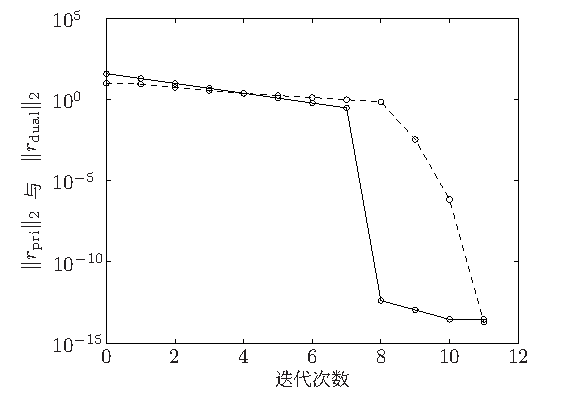
\includegraphics[width=.72\textwidth]{ch10-01.pdf}
\caption*{图10.1\quad 不可行初始点牛顿法求解具有100个变量、50个约束的等式约束解析中心问题的进展。图中给出 $\norm{r_{\rm pri}}_2$（实线）和 $\norm{r_{\rm dual}}_2$（虚线）。注意，第8次迭代后达到并保持可行；约从第9次迭代开始二次收敛。}
\end{figure}
\begin{figure}[htbp]\centering
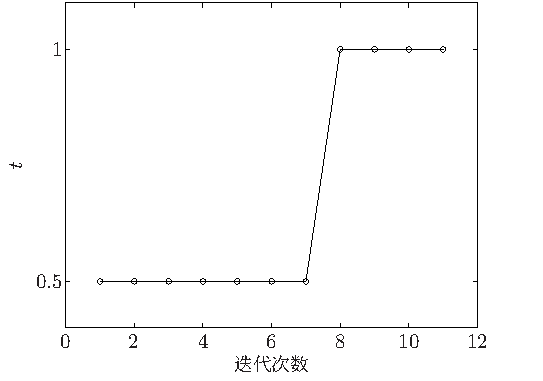
\includegraphics[width=.7\textwidth]{ch10-02.pdf}
\caption*{图10.2\quad 同一例题中步长随迭代次数的变化。第8次迭代取完整步，因此从第8次迭代开始可行。}
\end{figure}

% Source PDF page 558 (printed p. 544)
\begin{figure}[htbp]\centering
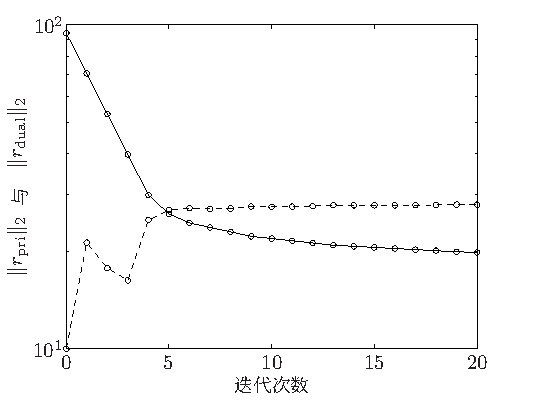
\includegraphics[width=.7\textwidth]{ch10-03.pdf}
\caption*{图10.3\quad 不可行初始点牛顿法求解具有100个变量、50个约束的等式约束解析中心问题的进展；该问题的 $\dom f=\R_{++}^{100}$ 与 $\{z\mid Az=b\}$ 不相交。图中给出 $\norm{r_{\rm pri}}_2$（实线）和 $\norm{r_{\rm dual}}_2$（虚线）。此时残差不收敛到零。}
\end{figure}
\begin{figure}[htbp]\centering
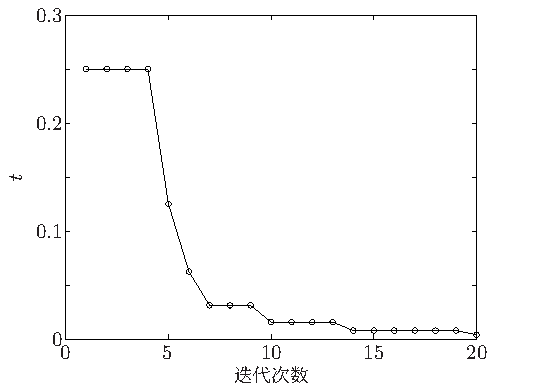
\includegraphics[width=.7\textwidth]{ch10-04.pdf}
\caption*{图10.4\quad 不可行例题中步长随迭代次数的变化。没有采用完整步，步长收敛到零。}
\end{figure}

% Source PDF page 559 (printed p. 545)
\begin{figure}[htbp]\centering
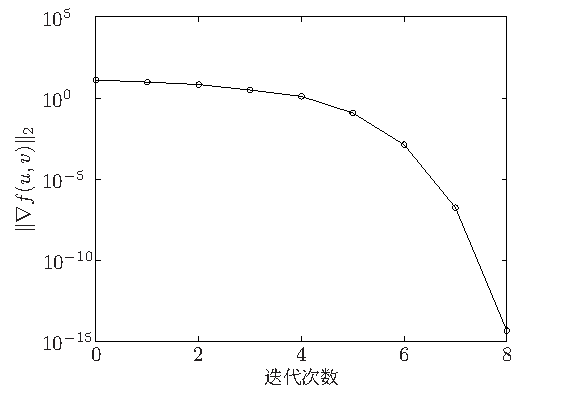
\includegraphics[width=.72\textwidth]{ch10-05.pdf}
\caption*{图10.5\quad 不可行初始点牛顿法求解凸凹博弈的进展。大约5次迭代后，二次收敛变得明显。}
\end{figure}
\begin{equation}\begin{bmatrix}H&A^\T\\A&0\end{bmatrix}\begin{bmatrix}v\\w\end{bmatrix}=-\begin{bmatrix}g\\h\end{bmatrix}.\tag{10.33}\end{equation}
假设 $H\in\mathbf S_+^n$，$A\in\R^{p\times n}$，且 $\rank A=p<n$。类似方法也可计算凸凹博弈的牛顿步，这时系数矩阵右下角分块是负半定的，见习题10.13。

\subsubsection*{求解完整 KKT 系统}
一种直接方法是求解整个 KKT 系统 (10.33)，即关于 $n+p$ 个变量的 $n+p$ 个线性方程。KKT 矩阵对称但不正定，因此适宜使用 $LDL^\T$ 分解，见第C.3.3节。如果不利用矩阵结构，代价为 $(1/3)(n+p)^3$ 次浮点运算。问题规模小，即 $n$、$p$ 不太大，或 $A$、$H$ 稀疏时，这可能是合理的方法。

\subsubsection*{通过消元求解 KKT 系统}
一种经常比直接求解完整 KKT 系统更好的方法，是消去变量 $v$，见第C.4节。先介绍最简单的 $H\succ0$ 的情况。由 KKT 方程
\[Hv+A^\T w=-g,\qquad Av=-h,\]
中的第一个方程解出 $v$：
\[v=-H^{-1}(g+A^\T w).\]

% Source PDF page 560 (printed p. 546)
代入第二个 KKT 方程，得到 $AH^{-1}(g+A^\T w)=h$，所以
\[w=(AH^{-1}A^\T)^{-1}(h-AH^{-1}g).\]
这些公式给出了计算 $v$ 和 $w$ 的方法。

$w$ 的表达式中出现的矩阵，是 $H$ 在 KKT 矩阵中的 Schur 补 $S$：
\[S=-AH^{-1}A^\T.\]
由于 KKT 矩阵的特殊结构，以及 $A$ 的秩为 $p$ 的假设，矩阵 $S$ 负定。

\begin{origalgorithm}{10.3}
\emph{用分块消元求解 KKT 系统。}

给定满足 $H\succ0$ 的 KKT 系统。
\begin{enumerate}
\item 形成 $H^{-1}A^\T$ 和 $H^{-1}g$。
\item 形成 Schur 补 $S=-AH^{-1}A^\T$。
\item 解 $Sw=AH^{-1}g-h$，得到 $w$。
\item 解 $Hv=-A^\T w-g$，得到 $v$。
\end{enumerate}
\end{origalgorithm}
第1步可通过 $H$ 的 Cholesky 分解，再进行 $p+1$ 次求解来完成，代价为 $f+(p+1)s$，其中 $f$ 是分解 $H$ 的代价，$s$ 是一次对应求解的代价。第2步需要一个 $p\times n$ 矩阵与 $n\times p$ 矩阵相乘。若不利用结构，代价为 $p^2n$ 次浮点运算；由于结果对称，只需计算 $S$ 的上三角部分。有时可以利用 $A$ 和 $H$ 的特殊结构，更高效地完成第2步。第3步可以对 $-S$ 作 Cholesky 分解；若不进一步利用 $S$ 的结构，代价为 $(1/3)p^3$。第4步可以使用第1步已计算的 $H$ 的分解，因此代价为 $2np+s$ 次浮点运算。假设在形成或分解 Schur 补时不利用结构，总浮点运算次数为
\[f+ps+p^2n+(1/3)p^3\]
（仅保留主项）。如果利用形成或分解 $S$ 时的结构，最后两项还会更小。

若 $H$ 可高效分解，分块消元的浮点运算次数就比用 $LDL^\T$ 分解直接求解 KKT 系统少。例如，若 $H$ 为对角矩阵，对应可分离目标函数，则 $f=0$、$s=n$，总代价为 $p^2n+(1/3)p^3$，仅随 $n$ 线性增长。若 $H$ 为带宽 $k\ll n$ 的带状矩阵，则 $f=nk^2$、$s=4nk$，总代价约为 $nk^2+4nkp+p^2n+(1/3)p^3$，仍仅随 $n$ 线性增长。$H$ 还可以有其他可利用的结构，如分块对角结构（对应分块可分离目标函数）、稀疏结构、对角加低秩结构；更多细节和例子见附录C与第9.7节。

\begin{origexample}{10.3}
\emph{等式约束解析中心。}考虑问题
\[\begin{array}{ll}\text{最小化}&-\displaystyle\sum_{i=1}^n\log x_i\\\text{约束条件}&Ax=b.\end{array}\]

% Source PDF page 561 (printed p. 547)
这里目标函数可分离，所以 $x$ 处的 Hessian 是对角矩阵：
\[H=\diag(x_1^{-2},\ldots,x_n^{-2}).\]
若用通用方法，如 KKT 矩阵的 $LDL^\T$ 分解计算牛顿方向，代价为 $(1/3)(n+p)^3$ 次浮点运算。

若用分块消元计算牛顿步，代价为 $np^2+(1/3)p^3$，比通用方法小得多。

事实上，这与第525页例10.2所述对偶问题中牛顿步的计算代价相同。对于该无约束对偶问题，Hessian 为
\[H_{\rm dual}=-ADA^\T,\]
其中 $D$ 是对角矩阵，$D_{ii}=(A^\T\nu)_i^{-2}$。形成该矩阵需要 $np^2$ 次浮点运算，对 $-H_{\rm dual}$ 作 Cholesky 分解来求牛顿步，需要 $(1/3)p^3$ 次浮点运算。
\end{origexample}

\begin{origexample}{10.4}
\emph{等式约束下的最短分段线性曲线。}考虑 $\R^2$ 中结点为 $(0,0),(1,x_1),\ldots,(n,x_n)$ 的分段线性曲线。为寻找满足等式约束 $Ax=b$ 的最短曲线，构造问题
\[\begin{array}{ll}\text{最小化}&(1+x_1^2)^{1/2}+\displaystyle\sum_{i=1}^{n-1}(1+(x_{i+1}-x_i)^2)^{1/2}\\\text{约束条件}&Ax=b,\end{array}\]
变量为 $x\in\R^n$，$A\in\R^{p\times n}$。目标为相邻变量对的函数之和，因此 Hessian $H$ 是三对角矩阵。用分块消元，可以约 $p^2n+(1/3)p^3$ 次浮点运算计算牛顿步。
\end{origexample}

\subsubsection*{$H$ 奇异时的消元}
上述分块消元法显然不适用于奇异 $H$，但只需简单修改，就可用于这一更一般情况。更一般的方法基于如下结果：KKT 矩阵非奇异，当且仅当对某个 $Q\succeq0$ 有 $H+A^\T QA\succ0$；此时对所有 $Q\succ0$ 都有 $H+A^\T QA\succ0$，见习题10.1。因此，例如，只要 KKT 矩阵非奇异，就有 $H+A^\T A\succ0$。

令 $Q\succeq0$ 为满足 $H+A^\T QA\succ0$ 的矩阵。KKT 系统 (10.33) 等价于
\[\begin{bmatrix}H+A^\T QA&A^\T\\A&0\end{bmatrix}\begin{bmatrix}v\\w\end{bmatrix}=-\begin{bmatrix}g+A^\T Qh\\h\end{bmatrix},\]
由于 $H+A^\T QA\succ0$，可以通过消元求解。

\subsection{例子}
本节给出一些较长的例子，说明怎样利用结构高效计算牛顿步，同时给出一些数值结果。

% Source PDF page 562 (printed p. 548)
\subsubsection*{等式约束解析中心}
考虑等式约束解析中心问题
\[\begin{array}{ll}\text{最小化}&f(x)=-\displaystyle\sum_{i=1}^n\log x_i\\\text{约束条件}&Ax=b.\end{array}\]
见例10.2和例10.3。对于 $p=100$、$n=500$ 的问题，比较三种方法。

第一种是带等式约束的牛顿法，第10.2节。牛顿步 $\Delta x_{\rm nt}$ 由 KKT 系统 (10.11) 定义：
\[\begin{bmatrix}H&A^\T\\A&0\end{bmatrix}\begin{bmatrix}\Delta x_{\rm nt}\\w\end{bmatrix}=\begin{bmatrix}-g\\0\end{bmatrix},\]
其中 $H=\diag(1/x_1^2,\ldots,1/x_n^2)$，$g=-(1/x_1,\ldots,1/x_n)$。如第546页例10.3解释的，可通过消元高效求解 KKT 系统，即求解
\[AH^{-1}A^\T w=-AH^{-1}g,\]
并令 $\Delta x_{\rm nt}=-H^{-1}(A^\T w+g)$。换言之，
\[\Delta x_{\rm nt}=-\diag(x)^2A^\T w+x,\]
其中 $w$ 为方程
\begin{equation}A\diag(x)^2A^\T w=b\tag{10.34}\end{equation}
的解。

图10.6给出误差随迭代次数的变化，不同曲线对应四个不同初始点。使用回溯参数 $\alpha=0.1$、$\beta=0.5$ 的线搜索。

第二种方法是对对偶问题使用牛顿法：
\[\text{最大化}\quad g(\nu)=-b^\T\nu+\sum_{i=1}^n\log(A^\T\nu)_i+n,\]
见第525页例10.2。这里通过求解
\begin{equation}A\diag(y)^2A^\T\Delta\nu_{\rm nt}=-b+Ay\tag{10.35}\end{equation}
得到牛顿步，其中 $y=(1/(A^\T\nu)_1,\ldots,1/(A^\T\nu)_n)$。比较 (10.35) 和 (10.34)，可见两种方法复杂度相同。图10.7给出四个不同初始点下的误差，回溯参数为 $\alpha=0.1$、$\beta=0.5$。

第三种是将第10.3节的不可行初始点牛顿法用于最优性条件
\[\nabla f(x^\star)+A^\T\nu^\star=0,\qquad Ax^\star=b.\]
牛顿步由求解
\[\begin{bmatrix}H&A^\T\\A&0\end{bmatrix}\begin{bmatrix}\Delta x_{\rm nt}\\\Delta\nu_{\rm nt}\end{bmatrix}=-\begin{bmatrix}g+A^\T\nu\\Ax-b\end{bmatrix}\]
得到。

% Source PDF page 563 (printed p. 549)
\begin{figure}[htbp]\centering
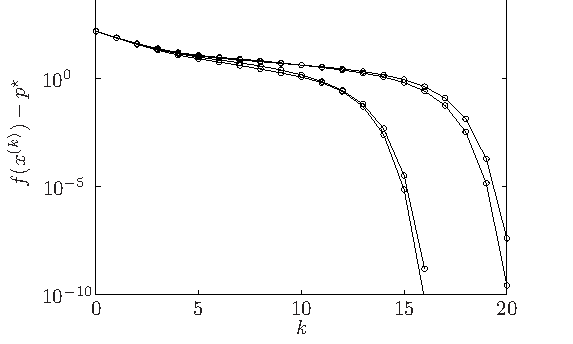
\includegraphics[width=.72\textwidth]{ch10-06.pdf}
\caption*{图10.6\quad 对大小为 $p=100$、$n=500$ 的等式约束解析中心问题使用牛顿法时的误差 $f(x^{(k)})-p^\star$。不同曲线对应四个不同初始点，最后的二次收敛清晰可见。}
\end{figure}
\begin{figure}[htbp]\centering
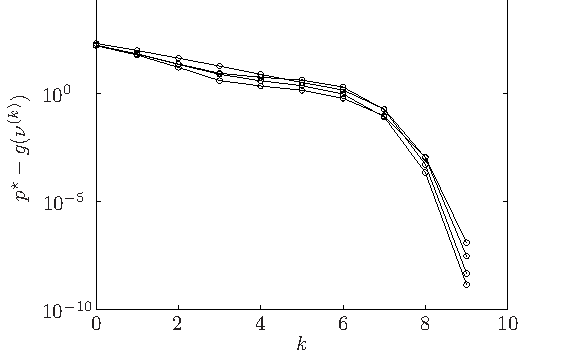
\includegraphics[width=.72\textwidth]{ch10-07.pdf}
\caption*{图10.7\quad 对等式约束解析中心问题的对偶使用牛顿法时的误差 $|g(\nu^{(k)})-p^\star|$。}
\end{figure}

% Source PDF page 564 (printed p. 550)
\begin{figure}[htbp]\centering
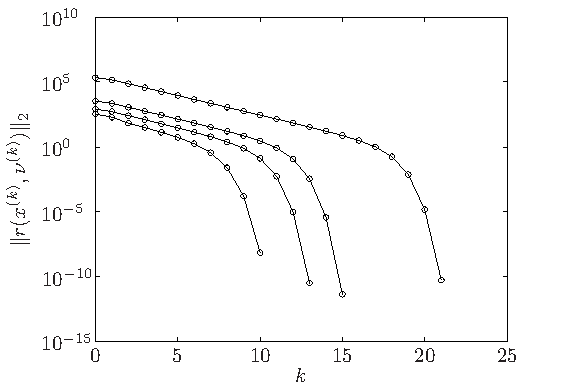
\includegraphics[width=.7\textwidth]{ch10-08.pdf}
\caption*{图10.8\quad 对等式约束解析中心问题使用不可行初始点牛顿法时的残差 $\norm{r(x^{(k)},\nu^{(k)})}_2$。}
\end{figure}
其中 $H=\diag(1/x_1^2,\ldots,1/x_n^2)$，$g=-(1/x_1,\ldots,1/x_n)$。这个 KKT 系统同样可以通过消元高效求解，代价与 (10.34) 或 (10.35) 相同。例如，先求解
\[A\diag(x)^2A^\T w=2Ax-b,\]
再由
\[\Delta\nu_{\rm nt}=w-\nu,\qquad\Delta x_{\rm nt}=x-\diag(x)^2A^\T w\]
得到 $\Delta\nu_{\rm nt}$ 与 $\Delta x_{\rm nt}$。图10.8给出四个不同初始点下残差
\[r(x,\nu)=(\nabla f(x)+A^\T\nu,Ax-b)\]
范数随迭代次数的变化，回溯参数为 $\alpha=0.1$、$\beta=0.5$。

图中可见，对这个问题，对偶方法似乎更快，但只快两三倍。它约经6次迭代进入二次收敛区域，而原始方法需12至15次，不可行初始点牛顿法需10至20次。

这些方法的初始化要求也不同。原始方法需要一个已知原始可行点，即满足 $Ax^{(0)}=b$、$x^{(0)}\succ0$。对偶方法需要一个对偶可行点，即 $A^\T\nu^{(0)}\succ0$。依具体问题不同，二者之一可能更容易获得。不可行初始点牛顿法不需要这样的初始化，唯一要求是 $x^{(0)}\succ0$。

\subsubsection*{最优网络流}
考虑具有 $n$ 条边、$p+1$ 个结点的连通有向图或网络。用 $x_j$ 表示弧 $j$ 上的流量或交通量，$x_j>0$ 表示沿弧方向流动。

% Source PDF page 565 (printed p. 551)
$x_j<0$ 表示沿弧的反方向流动。此外，给定外部源或汇流量 $s_i$：$s_i>0$ 时进入结点 $i$，$s_i<0$ 时离开结点 $i$。流量必须满足守恒方程，即每个结点的总净流入（包括外部源和汇）为零。守恒方程可写为 $\widetilde Ax=s$，其中 $\widetilde A\in\R^{(p+1)\times n}$ 是图的结点关联矩阵：
\[\widetilde A_{ij}=\begin{cases}1,&\text{弧 }j\text{ 离开结点 }i,\\-1,&\text{弧 }j\text{ 进入结点 }i,\\0,&\text{其他情形}.\end{cases}\]
流量守恒方程 $\widetilde Ax=s$ 只有在 $\one^\T s=0$ 时才可能相容，这里假定此条件成立。换言之，源流量总和必须等于汇流量总和。由于 $\one^\T\widetilde A=0$，方程 $\widetilde Ax=s$ 也存在冗余。为了得到独立方程组，可以删去其中任意一个方程，得到 $Ax=b$；其中 $A\in\R^{p\times n}$ 是图的约化结点关联矩阵，即删去一行的结点关联矩阵，$b\in\R^p$ 是约化源向量，即删去对应元素的 $s$。

总之，流量守恒由 $Ax=b$ 给出，其中 $A$ 是图的约化结点关联矩阵，$b$ 是约化源向量。矩阵 $A$ 非常稀疏，每列至多有两个非零元素，且只能为 $+1$ 或 $-1$。

以流量 $x$ 为变量，源流量已知。引入目标函数
\[f(x)=\sum_{i=1}^n\phi_i(x_i),\]
其中 $\phi_i:\R\to\R$ 是弧 $i$ 的流量代价函数。假设流量代价函数严格凸且二阶可微。

满足流量守恒要求的最佳流量选择问题为
\begin{equation}\begin{array}{ll}\text{最小化}&\displaystyle\sum_{i=1}^n\phi_i(x_i)\\\text{约束条件}&Ax=b.\end{array}\tag{10.36}\end{equation}
由于目标函数可分离，Hessian $H$ 为对角矩阵。

计算最优网络流问题 (10.36) 的牛顿步有几种选择。最直接的是用稀疏 $LDL^\T$ 分解求解完整 KKT 系统。

对这个问题，用分块消元计算牛顿步可能更好。Schur 补 $S=-AH^{-1}A^\T$ 的稀疏模式可以用图描述：$S_{ij}\ne0$ 当且仅当结点 $i$ 与 $j$ 由一条弧连接。因此，如果网络稀疏，即每个结点只通过弧与少数其他结点连接，那么 Schur 补 $S$ 也稀疏。此时，在形成 $S$、以及对应的分解与求解步骤中，都可利用稀疏性。可以预期牛顿步的计算复杂度约随弧数，也就是变量数，线性增长。

% Source PDF page 566 (printed p. 552)
\subsubsection*{最优控制}
考虑问题
\[\begin{array}{ll}\text{最小化}&\displaystyle\sum_{t=1}^N\phi_t(z(t))+\sum_{t=0}^{N-1}\psi_t(u(t))\\\text{约束条件}&z(t+1)=A_tz(t)+B_tu(t),\quad t=0,\ldots,N-1.\end{array}\]
其中
\begin{itemize}
\item $z(t)\in\R^k$ 是时刻 $t$ 的系统状态；
\item $u(t)\in\R^l$ 是时刻 $t$ 的输入或控制作用；
\item $\phi_t:\R^k\to\R$ 是状态代价函数；
\item $\psi_t:\R^l\to\R$ 是输入代价函数；
\item $N$ 称为问题的时间范围。
\end{itemize}
假设输入代价与状态代价函数严格凸且二阶可微。问题变量为 $u(0),\ldots,u(N-1)$ 和 $z(1),\ldots,z(N)$。初始状态 $z(0)$ 已知。线性等式约束称为状态方程或动态演化方程。定义整体优化变量
\[x=(u(0),z(1),u(1),\ldots,u(N-1),z(N))\in\R^{N(k+l)}.\]
由于目标函数分块可分离，即为 $z(t)$ 和 $u(t)$ 的函数之和，Hessian 为分块对角矩阵：
\[H=\diag(R_0,Q_1,\ldots,R_{N-1},Q_N),\]
其中
\[\begin{aligned}
R_t&=\nabla^2\psi_t(u(t)),&&t=0,\ldots,N-1,\\
Q_t&=\nabla^2\phi_t(z(t)),&&t=1,\ldots,N.
\end{aligned}\]
将所有等式约束，即状态方程，合并为 $Ax=b$，其中
\begingroup\small
\[
A=\begin{bmatrix}
-B_0&I&0&0&0&\cdots&0&0&0\\
0&-A_1&-B_1&I&0&\cdots&0&0&0\\
0&0&0&-A_2&-B_2&\cdots&0&0&0\\
\vdots&\vdots&\vdots&\vdots&\vdots&&\vdots&\vdots&\vdots\\
0&0&0&0&0&\cdots&I&0&0\\
0&0&0&0&0&\cdots&-A_{N-1}&-B_{N-1}&I
\end{bmatrix},\qquad
b=\begin{bmatrix}A_0z(0)\\0\\0\\\vdots\\0\\0\end{bmatrix}.
\]
\endgroup

% Source PDF page 567 (printed p. 553)
$A$ 的行数，即等式约束数，为 $Nk$。

若用稠密 $LDL^\T$ 分解直接求解牛顿步的 KKT 系统，代价为
\[(1/3)(2Nk+Nl)^3=(1/3)N^3(2k+l)^3\]
次浮点运算。使用稀疏 $LDL^\T$ 分解会有很大改进，因为它能利用 $A$ 和 $H$ 中的大量零元素。

事实上，通过分块消元计算牛顿步，并利用 $H$ 和 $A$ 的特殊分块结构，可以做得更好。Schur 补 $S=-AH^{-1}A^\T$ 是以 $k\times k$ 矩阵为分块的分块三对角矩阵：
\begingroup\small
\[
\begin{aligned}
S&=-AH^{-1}A^\T\\
&=\begin{bmatrix}
S_{11}&Q_1^{-1}A_1^\T&0&\cdots&0&0\\
A_1Q_1^{-1}&S_{22}&Q_2^{-1}A_2^\T&\cdots&0&0\\
0&A_2Q_2^{-1}&S_{33}&\cdots&0&0\\
\vdots&\vdots&\vdots&\ddots&\vdots&\vdots\\
0&0&0&\cdots&S_{N-1,N-1}&Q_{N-1}^{-1}A_{N-1}^\T\\
0&0&0&\cdots&A_{N-1}Q_{N-1}^{-1}&S_{NN}
\end{bmatrix},
\end{aligned}\]
\endgroup
其中
\[\begin{aligned}
S_{11}&=-B_0R_0^{-1}B_0^\T-Q_1^{-1},\\
S_{ii}&=-A_{i-1}Q_{i-1}^{-1}A_{i-1}^\T-B_{i-1}R_{i-1}^{-1}B_{i-1}^\T-Q_i^{-1},&&i=2,\ldots,N.
\end{aligned}\]
特别地，$S$ 为带宽 $2k-1$ 的带状矩阵，因此可用 $k^3N$ 量级的浮点运算分解它。假设 $k\ll N$，便能以 $k^3N$ 量级的浮点运算计算牛顿步。注意，这随时间范围 $N$ 线性增长，而通用方法的浮点运算次数随 $N^3$ 增长。

对这个问题还可以进一步利用 $S$ 的分块三对角结构。应用标准分块三对角分解方法，会得到求解二次最优控制问题的经典 Riccati 递推。不过，即使只利用 $S$ 的带状性质，也能得到同阶算法。

\subsubsection*{线性矩阵不等式的解析中心}
考虑问题
\begin{equation}\begin{array}{ll}\text{最小化}&f(X)=-\log\det X\\\text{约束条件}&\tr(A_iX)=b_i,\quad i=1,\ldots,p,\end{array}\tag{10.37}\end{equation}
其中 $X\in\mathbf S^n$ 为变量，$A_i\in\mathbf S^n$、$b_i\in\R$，$\dom f=\mathbf S_{++}^n$。该问题的 KKT 条件为
\begin{equation}-X^{\star-1}+\sum_{i=1}^m\nu_i^\star A_i=0,\qquad\tr(A_iX^\star)=b_i,\quad i=1,\ldots,p.\tag{10.38}\end{equation}
变量 $X$ 的维数为 $n(n+1)/2$。可以简单地忽略 $X$ 的特殊矩阵结构，将其看成向量变量 $x\in\R^{n(n+1)/2}$，并对一个具有 $n(n+1)/2$ 个变量和 $p$ 个等式约束的问题使用通用方法求解 (10.37)。

% Source PDF page 568 (printed p. 554)
此时计算牛顿步的代价至少为
\[(1/3)(n(n+1)/2+p)^3\]
次浮点运算，关于 $n$ 为 $n^6$ 量级。下面将看到几种好得多的替代方案。

第一种选择是求解对偶问题。$f$ 的共轭为
\[f^*(Y)=\log\det(-Y)^{-1}-n,\]
定义域为 $\dom f^*=-\mathbf S_{++}^n$，见第92页例3.23，因此对偶问题为
\begin{equation}\text{最大化}\quad-b^\T\nu+\log\det\left(\sum_{i=1}^p\nu_iA_i\right)+n,\tag{10.39}\end{equation}
定义域为 $\{\nu\mid\sum_{i=1}^p\nu_iA_i\succ0\}$。这是变量为 $\nu\in\R^p$ 的无约束问题。由最优 $\nu^\star$，可通过求解 (10.38) 中第一个对偶可行性方程恢复最优 $X^\star$，即 $X^\star=(\sum_{i=1}^p\nu_i^\star A_i)^{-1}$。

计算对偶问题 (10.39) 的牛顿步，需要形成 $g$ 的梯度和 Hessian，再求出牛顿步。梯度与 Hessian 为
\[\begin{aligned}
\nabla^2g(\nu)_{ij}&=-\tr(A^{-1}A_iA^{-1}A_j),&&i,j=1,\ldots,p,\\
\nabla g(\nu)_i&=\tr(A^{-1}A_i)-b_i,&&i=1,\ldots,p,
\end{aligned}\]
其中 $A=\sum_{i=1}^p\nu_iA_i$。为形成 $\nabla^2g(\nu)$ 与 $\nabla g(\nu)$，先形成 $A$，代价为 $pn^2$ 次浮点运算，再对各个 $j$ 形成 $A^{-1}A_j$，代价为 $2pn^3$。然后形成矩阵 $\nabla^2g(\nu)$。其 $p(p+1)/2$ 个元素中的每一个，都是两个 $\mathbf S^n$ 矩阵的内积，每次需要 $n(n+1)$ 次浮点运算，因此总计为 $(1/2)p^2n^2$，这里忽略低阶项。由于已经得到矩阵 $A^{-1}A_i$，形成 $\nabla g(\nu)$ 代价很小。最后，求解牛顿步 $-\nabla^2g(\nu)^{-1}\nabla g(\nu)$，代价为 $(1/3)p^3$。合起来只保留主项，牛顿步的总计算代价为 $2pn^3+(1/2)p^2n^2+(1/3)p^3$。注意，这关于 $n$ 为 $n^3$ 量级，远优于上面 $n^6$ 量级的简单原始方法。

也可以利用原始问题的特殊矩阵结构，更高效地求解它。为推导可行 $X$ 处牛顿步 $\Delta X_{\rm nt}$ 的 KKT 系统，在 KKT 条件中用 $X+\Delta X_{\rm nt}$ 代替 $X^\star$，用 $w$ 代替 $\nu^\star$，并用一阶近似
\[(X+\Delta X_{\rm nt})^{-1}\approx X^{-1}-X^{-1}\Delta X_{\rm nt}X^{-1}\]
线性化第一个方程，得到 KKT 系统
\begin{equation}\begin{gathered}
-X^{-1}+X^{-1}\Delta X_{\rm nt}X^{-1}+\sum_{i=1}^p w_iA_i=0,\\
\tr(A_i\Delta X_{\rm nt})=0,\quad i=1,\ldots,p.
\end{gathered}\tag{10.40}\end{equation}
这是一组关于变量 $\Delta X_{\rm nt}\in\mathbf S^n$ 与 $w\in\R^p$ 的 $n(n+1)/2+p$ 个线性方程。若用通用方法求解，代价为 $n^6$ 量级。

% Source PDF page 569 (printed p. 555)
可以用分块消元更高效地求解 KKT 系统 (10.40)。由第一个方程解出 $\Delta X_{\rm nt}$，消去这个变量：
\begin{equation}\Delta X_{\rm nt}=X-X\left(\sum_{i=1}^p w_iA_i\right)X=X-\sum_{i=1}^p w_iXA_iX.\tag{10.41}\end{equation}
将该表达式代入另一个方程，得到
\[\tr(A_j\Delta X_{\rm nt})=\tr(A_jX)-\sum_{i=1}^p w_i\tr(A_jXA_iX)=0,\qquad j=1,\ldots,p.\]
这是关于 $w$ 的 $p$ 个线性方程：
\[Cw=d,\]
其中 $C_{ij}=\tr(A_iXA_jX)$、$d_i=\tr(A_iX)$。系数矩阵 $C$ 对称正定，因此可以用 Cholesky 分解求 $w$。得到 $w$ 后，就能由 (10.41) 计算 $\Delta X_{\rm nt}$。

该方法的代价如下。先形成乘积 $A_iX$，需要 $2pn^3$ 次浮点运算，再形成矩阵 $C$。$C$ 的 $p(p+1)/2$ 个元素中的每一个，都是两个 $\R^{n\times n}$ 矩阵的内积，因此形成 $C$ 需要 $p^2n^2$ 次浮点运算。然后求 $w=C^{-1}d$，需要 $(1/3)p^3$。最后计算 $\Delta X_{\rm nt}$。若使用 (10.41) 中第一个表达式，即先求和，再在左右分别乘以 $X$，代价约为 $pn^2+3n^3$。总之，采用分块消元形成原始问题牛顿步的总浮点运算次数为 $2pn^3+p^2n^2+(1/3)p^3$，远优于 $n^6$ 量级的简单方法。注意，这也与计算对偶问题牛顿步的代价相同。

% Source PDF page 570 (printed p. 556)
\section*{文献说明}
\addcontentsline{toc}{section}{文献说明}
分析不可行初始点牛顿法时所用的两个关键假设，即导数 $Dr$ 的逆有界以及满足 Lipschitz 条件，也是大多数牛顿法收敛证明的核心；见 Ortega 与 Rheinboldt [OR00]、Dennis 与 Schnabel [DS96]。

在用于线性规划与二次规划的内点法中，对直接分解完整 KKT 系统和通过消元求解 KKT 系统的相对优劣，已有广泛研究；例如见 Wright [Wri97, 第11章]、Nocedal 与 Wright [NW99, 第16.1--2节]。最优控制中的 Riccati 递推，可以解释为利用第552页例子中 Schur 补 $S$ 的分块三对角结构的方法。Rao、Wright 与 Rawlings [RWR98, 第3.3节] 作出了这一观察。

% Source PDF page 571 (printed p. 557)
\section*{习题}
\addcontentsline{toc}{section}{习题}
\subsection*{等式约束最小化}
\paragraph{10.1} \emph{KKT 矩阵的非奇异性。}考虑 KKT 矩阵
\[\begin{bmatrix}P&A^\T\\A&0\end{bmatrix},\]
其中 $P\in\mathbf S_+^n$、$A\in\R^{p\times n}$，$\rank A=p<n$。
\begin{enumerate}[label=(\alph*)]
\item 证明以下每一个陈述都与 KKT 矩阵非奇异等价：
\begin{itemize}
\item $\mathcal N(P)\cap\mathcal N(A)=\{0\}$。
\item $Ax=0$、$x\ne0\Longrightarrow x^\T Px>0$。
\item $F^\T PF\succ0$，其中 $F\in\R^{n\times(n-p)}$ 满足 $\mathcal R(F)=\mathcal N(A)$。
\item 对某个 $Q\succeq0$，有 $P+A^\T QA\succ0$。
\end{itemize}
\item 证明，若 KKT 矩阵非奇异，则它恰有 $n$ 个正特征值和 $p$ 个负特征值。
\end{enumerate}

\paragraph{10.2} \emph{投影梯度法。}本题探索梯度法在等式约束最小化中的扩展。假设 $f$ 凸且可微，$x\in\dom f$ 满足 $Ax=b$，其中 $A\in\R^{p\times n}$，$\rank A=p<n$。负梯度 $-\nabla f(x)$ 在 $\mathcal N(A)$ 上的欧几里得投影为
\[\Delta x_{\rm pg}=\argmin_{Au=0}\norm{-\nabla f(x)-u}_2.\]
\begin{enumerate}[label=(\alph*)]
\item 设 $(v,w)$ 是
\[\begin{bmatrix}I&A^\T\\A&0\end{bmatrix}\begin{bmatrix}v\\w\end{bmatrix}=\begin{bmatrix}-\nabla f(x)\\0\end{bmatrix}\]
的唯一解。证明 $v=\Delta x_{\rm pg}$，且 $w=\argmin_y\norm{\nabla f(x)+A^\T y}_2$。
\item 假设 $F^\T F=I$，投影负梯度 $\Delta x_{\rm pg}$ 与约化问题 (10.5) 的负梯度有什么关系？
\item 求解等式约束最小化问题的投影梯度法，使用步 $\Delta x_{\rm pg}$，并对 $f$ 作回溯线搜索。利用 (b) 的结果，给出从满足 $Ax^{(0)}=b$ 的 $x^{(0)}\in\dom f$ 出发时，投影梯度法收敛到最优解的一些条件。
\end{enumerate}

\subsection*{带等式约束的牛顿法}
\paragraph{10.3} \emph{对偶牛顿法。}本题研究用牛顿法求解等式约束最小化问题 (10.1) 的对偶。假设 $f$ 二阶可微，所有 $x\in\dom f$ 都满足 $\nabla^2f(x)\succ0$，而且对每个 $\nu\in\R^p$，拉格朗日函数 $L(x,\nu)=f(x)+\nu^\T(Ax-b)$ 都有唯一最小化点，记为 $x(\nu)$。
\begin{enumerate}[label=(\alph*)]
\item 证明对偶函数 $g$ 二阶可微。用 $f$、$\nabla f$、$\nabla^2f$ 在 $x=x(\nu)$ 处的值，写出对偶函数 $g$ 在 $\nu$ 处的牛顿步。可以使用习题3.40的结果。
\end{enumerate}

% Source PDF page 572 (printed p. 558)
\begin{enumerate}[label=(\alph*),start=2]
\item 假设存在 $K$，使对所有 $x\in\dom f$ 都有
\[\left\|\begin{bmatrix}\nabla^2f(x)&A^\T\\A&0\end{bmatrix}^{-1}\right\|_2\le K.\]
证明 $g$ 强凹，且 $\nabla^2g(\nu)\preceq-(1/K)I$。
\end{enumerate}

\paragraph{10.4} \emph{约化问题的强凸性与 Lipschitz 常数。}假设 $f$ 满足第529页的假设。证明约化目标函数 $\widetilde f(z)=f(Fz+\widehat x)$ 强凸，且其 Hessian 在相应下水平集 $\widetilde S$ 上 Lipschitz 连续。用 $K,M,L$ 以及 $F$ 的最大、最小奇异值，表达 $\widetilde f$ 的强凸性常数与 Lipschitz 常数。

\paragraph{10.5} \emph{给目标增加二次项。}假设 $Q\succeq0$。问题
\[\begin{array}{ll}\text{最小化}&f(x)+(Ax-b)^\T Q(Ax-b)\\\text{约束条件}&Ax=b\end{array}\]
等价于原等式约束优化问题 (10.1)。该问题的牛顿步与原问题的牛顿步是否相同？

\paragraph{10.6} \emph{牛顿减量。}证明 (10.13) 成立，即
\[f(x)-\inf\{\widehat f(x+v)\mid A(x+v)=b\}=\lambda(x)^2/2.\]

\subsection*{不可行初始点牛顿法}
\paragraph{10.7} \emph{不可行初始点牛顿法的假设。}考虑第536页的假设。
\begin{enumerate}[label=(\alph*)]
\item 假设函数 $f$ 是闭函数。证明这蕴含残差范数 $\norm{r(x,\nu)}_2$ 是闭函数。
\item 证明 $Dr$ 满足 Lipschitz 条件，当且仅当 $\nabla^2f$ 满足 Lipschitz 条件。
\end{enumerate}

\paragraph{10.8} \emph{不可行初始点牛顿法与初始已满足的等式约束。}假设用不可行初始点牛顿法，在 $a_i^\T x=b_i$（$i=1,\ldots,p$）下最小化 $f(x)$。
\begin{enumerate}[label=(\alph*)]
\item 假设初始点 $x^{(0)}$ 满足线性等式 $a_i^\T x=b_i$。证明此后所有迭代点都满足该等式，即对所有 $k$ 有 $a_i^\T x^{(k)}=b_i$。
\item 假设某个等式约束在第 $k$ 次迭代首次满足，即 $a_i^\T x^{(k-1)}\ne b_i$、$a_i^\T x^{(k)}=b_i$。证明在第 $k$ 次迭代，全部等式约束都满足。
\end{enumerate}

\paragraph{10.9} \emph{等式约束熵最大化。}考虑等式约束熵最大化问题
\begin{equation}\begin{array}{ll}\text{最小化}&f(x)=\displaystyle\sum_{i=1}^n x_i\log x_i\\\text{约束条件}&Ax=b,\end{array}\tag{10.42}\end{equation}
其中 $\dom f=\R_{++}^n$，$A\in\R^{p\times n}$。假设问题可行，$\rank A=p<n$。
\begin{enumerate}[label=(\alph*)]
\item 证明问题具有唯一最优解 $x^\star$。
\item 寻找 $A,b$ 与可行 $x^{(0)}$，使下水平集
\[\{x\in\R_{++}^n\mid Ax=b,\ f(x)\le f(x^{(0)})\}\]
不闭。因此，对于某些可行初始点，第10.2.4节（第529页）的假设不成立。
\end{enumerate}

% Source PDF page 573 (printed p. 559)
\begin{enumerate}[label=(\alph*),start=3]
\item 证明，对任何可行初始点，问题 (10.42) 都满足第10.3.3节（第536页）列出的不可行初始点牛顿法假设。
\item 推导 (10.42) 的拉格朗日对偶，并说明如何由对偶问题最优解求 (10.42) 的最优解。证明对任何初始点，对偶问题都满足第10.2.4节（第529页）列出的假设。
\end{enumerate}
(b)、(c)、(d) 的结果并不意味着标准牛顿法会失败，也不意味着不可行初始点牛顿法或对偶方法在实际中表现更好。它们只表明，这里的标准牛顿法收敛分析不适用，而不可行初始点与对偶方法的收敛分析适用。（见习题10.15。）

\paragraph{10.10} \emph{强凸凹博弈的导数逆有界条件。}考虑收益函数为 $f$ 的凸凹博弈，见第541页。假设对所有 $(u,v)\in\dom f$，有 $\nabla_{uu}^2f(u,v)\succeq mI$ 和 $\nabla_{vv}^2f(u,v)\preceq-mI$。证明
\[\norm{Dr(u,v)^{-1}}_2=\norm{\nabla^2f(u,v)^{-1}}_2\le1/m.\]

\subsection*{实现}
\paragraph{10.11} 考虑例10.1的资源分配问题。可假设 $f_i$ 强凸，即所有 $z$ 都有 $f_i''(z)\ge m>0$。
\begin{enumerate}[label=(\alph*)]
\item 求计算约化问题牛顿步所需的计算量，务必利用牛顿方程的特殊结构。
\item 说明如何通过对偶求解。可以假设共轭函数 $f_i^*$ 及其导数容易计算，而且给定 $\nu$ 时，方程 $f_i'(x)=\nu$ 容易对 $x$ 求解。求对偶问题牛顿步的计算复杂度是多少？
\item 计算资源分配问题牛顿步的复杂度是多少？务必利用 KKT 方程的特殊结构。
\end{enumerate}

\paragraph{10.12} 描述一种高效计算以下问题牛顿步的方法：
\[\begin{array}{ll}\text{最小化}&\tr(X^{-1})\\\text{约束条件}&\tr(A_iX)=b_i,\quad i=1,\ldots,p,\end{array}\]
定义域为 $\mathbf S_{++}^n$，假设 $p$ 与 $n$ 同阶。并推导拉格朗日对偶问题，给出求对偶问题牛顿步的复杂度。

\paragraph{10.13} \emph{用消元法计算凸凹博弈的牛顿步。}考虑收益函数 $f:\R^p\times\R^q\to\R$ 的凸凹博弈，见第541页。假设 $f$ 强凸凹，即对所有 $(u,v)\in\dom f$ 与某个 $m>0$，有 $\nabla_{uu}^2f(u,v)\succeq mI$ 和 $\nabla_{vv}^2f(u,v)\preceq-mI$。
\begin{enumerate}[label=(\alph*)]
\item 说明如何使用 $\nabla_{uu}^2f(u,v)$ 与 $-\nabla_{vv}^2f(u,v)$ 的 Cholesky 分解计算牛顿步。假设 $\nabla^2f(u,v)$ 稠密，比较这一方法与对 $\nabla f(u,v)$ 作 $LDL^\T$ 分解的代价。
\item 说明如何利用 $\nabla_{uu}^2f(u,v)$ 和／或 $\nabla_{vv}^2f(u,v)$ 的对角或分块对角结构。假设 $\nabla_{uv}^2f(u,v)$ 稠密，可以节省多少计算？
\end{enumerate}

\subsection*{数值实验}
\paragraph{10.14} \emph{对数最优投资。}考虑习题4.60所述的对数最优投资问题，去掉约束 $x\succeq0$。使用牛顿法求解，问题数据如下。

% Source PDF page 574 (printed p. 560)
有 $n=3$ 种资产、$m=4$ 种情景，收益为
\[p_1=\begin{bmatrix}2\\1.3\\1\end{bmatrix},\qquad p_2=\begin{bmatrix}2\\0.5\\1\end{bmatrix},\qquad p_3=\begin{bmatrix}0.5\\1.3\\1\end{bmatrix},\qquad p_4=\begin{bmatrix}0.5\\0.5\\1\end{bmatrix}.\]
四个情景的概率为 $\pi=(1/3,1/6,1/3,1/6)$。

\paragraph{10.15} \emph{等式约束熵最大化。}考虑等式约束熵最大化问题
\[\begin{array}{ll}\text{最小化}&f(x)=\displaystyle\sum_{i=1}^n x_i\log x_i\\\text{约束条件}&Ax=b,\end{array}\]
其中 $\dom f=\R_{++}^n$，$A\in\R^{p\times n}$，$p<n$。（相关分析见习题10.9。）

生成一个 $n=100$、$p=30$ 的实例：随机选择 $A$ 并检查其满秩，选随机正向量 $\widehat x$，例如各元素在 $[0,1]$ 上均匀分布，再令 $b=A\widehat x$，于是 $\widehat x$ 可行。

采用以下方法计算问题的解。
\begin{enumerate}[label=(\alph*)]
\item 标准牛顿法。可取初始点 $x^{(0)}=\widehat x$。
\item 不可行初始点牛顿法。可取 $x^{(0)}=\widehat x$ 以便与标准牛顿法比较，也可取 $x^{(0)}=\one$。
\item 对偶牛顿法，即对对偶问题采用标准牛顿法。
\end{enumerate}
验证三个方法得到相同最优点及拉格朗日乘子。假设利用了相关结构，比较三种方法每步的计算量；不过，实现时并不要求利用结构计算牛顿步。

\paragraph{10.16} \emph{凸凹博弈。}对随机生成的数据，使用不可行初始点牛顿法求解形如 (10.32) 的凸凹博弈。绘出残差范数及步长随迭代次数的变化。尝试不同的线搜索参数和初始点，但初始点必须满足 $\norm u_2<1$、$\norm v_2<1$。


\chapter{内点法}
% Source PDF page 575 (printed p. 561)
\section{不等式约束最小化问题}
本章讨论求解含不等式约束的凸优化问题的内点法：
\begin{equation}\begin{aligned}
\text{最小化}\quad &f_0(x)\\
\text{约束为}\quad &f_i(x)\le0,\quad i=1,\ldots,m,\\
&Ax=b,
\end{aligned}\tag{11.1}\end{equation}
其中 $f_0,\ldots,f_m:\R^n\to\R$ 为凸且二阶连续可微函数，$A\in\R^{p\times n}$，并且 $\rank A=p<n$。假设该问题可解，即存在最优解 $x^\star$，以 $p^\star$ 表示最优值 $f_0(x^\star)$。

还假设该问题严格可行，即存在 $x\in\mathcal D$，满足 $Ax=b$ 以及 $f_i(x)<0$，$i=1,\ldots,m$。这意味着 Slater 约束资格条件成立，因而存在对偶最优解 $\lambda^\star\in\R^m$、$\nu^\star\in\R^p$，它们与 $x^\star$ 一起满足 KKT 条件
\begin{equation}\begin{aligned}
Ax^\star&=b,\qquad f_i(x^\star)\le0,\quad i=1,\ldots,m,\\
\lambda^\star&\succeq0,\\
\nabla f_0(x^\star)+\sum_{i=1}^m\lambda_i^\star\nabla f_i(x^\star)+A^\T\nu^\star&=0,\\
\lambda_i^\star f_i(x^\star)&=0,\quad i=1,\ldots,m.
\end{aligned}\tag{11.2}\end{equation}
内点法将牛顿法应用于一系列等式约束问题，或一系列修改后的 KKT 条件，从而求解问题 (11.1)（或 KKT 条件 (11.2)）。我们将重点讨论一种具体的内点算法——障碍法，并给出其收敛性证明与复杂度分析。还将在第11.7节介绍一种简单的原始—对偶内点法，但不作分析。

可以把内点法看作凸优化算法层次中的又一层。最简单的是线性等式约束二次问题。对这类问题，KKT 条件是一组线性方程，可以解析求解。牛顿法处于下一层。可以认为，牛顿法通过将具有二阶可微目标函数的线性等式约束优化问题化为一系列线性等式约束二次问题，来求解前者。
% Source PDF page 576 (printed p. 562)
内点法则再进一层：它将带有线性等式约束和不等式约束的优化问题，化为一系列线性等式约束问题来求解。

\subsection*{例子}
许多问题已经具有 (11.1) 的形式，而且满足目标函数与约束函数二阶可微的假设。明显的例子包括 LP、QP、QCQP 以及凸形式的 GP；另一个例子是带线性不等式约束的熵最大化问题，
\[
\begin{aligned}
\text{最小化}\quad&\sum_{i=1}^n x_i\log x_i\\
\text{约束为}\quad&Fx\preceq g,\\
&Ax=b,
\end{aligned}
\]
其定义域为 $\mathcal D=\R_{++}^n$。

另外许多问题并不具有要求的 (11.1) 形式，其目标函数和约束函数也不是二阶可微的，但可以重新表述成所需形式。我们已经见过许多这样的例子，例如，将无约束凸分段线性最小化问题
\[
\text{最小化}\quad\max_{i=1,\ldots,m}(a_i^\T x+b_i)
\]
（其目标函数不可微）转化为 LP
\[
\begin{aligned}
\text{最小化}\quad&t\\
\text{约束为}\quad&a_i^\T x+b_i\le t,\quad i=1,\ldots,m
\end{aligned}
\]
（其目标函数和约束函数都是二阶可微的）。

有些凸优化问题，例如 SOCP 和 SDP，不容易改写为所需形式，但可以用处理广义不等式问题的内点法扩展来求解。第11.6节将介绍这种扩展。

\section{对数障碍函数与中心路径}
我们的目标是把不等式约束问题 (11.1) 近似表述为可应用牛顿法的等式约束问题。第一步是将不等式约束隐含在目标函数中，把问题 (11.1) 改写为
\begin{equation}\begin{aligned}
\text{最小化}\quad&f_0(x)+\sum_{i=1}^m I_-(f_i(x))\\
\text{约束为}\quad&Ax=b,
\end{aligned}\tag{11.3}\end{equation}
其中 $I_-:\R\to\R$ 是非正实数集的示性函数：
\[
I_-(u)=\begin{cases}0,&u\le0,\\\infty,&u>0.\end{cases}
\]
% Source PDF page 577 (printed p. 563)
\begin{figure}[htbp]\centering
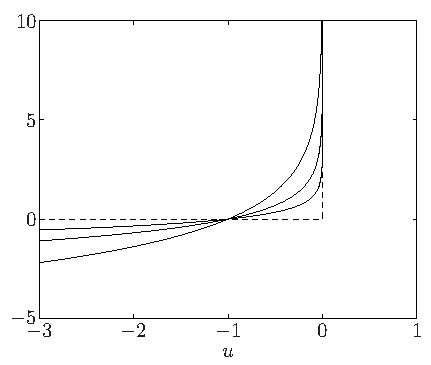
\includegraphics[width=.55\textwidth]{figures/ch11-01.pdf}
\caption*{图11.1 虚线表示函数 $I_-(u)$，实线表示 $\widehat I_-(u)=-(1/t)\log(-u)$，其中 $t=0.5,1,2$。$t=2$ 对应的曲线给出最好的近似。}
\end{figure}
问题 (11.3) 没有不等式约束，但其目标函数一般不可微，因此不能应用牛顿法。

\subsection{对数障碍}
障碍法的基本思想是用函数
\[
\widehat I_-(u)=-(1/t)\log(-u),\qquad\dom\widehat I_-=-\R_{++}
\]
近似示性函数 $I_-$，其中参数 $t>0$ 决定近似的精度。与 $I_-$ 一样，$\widehat I_-$ 为凸且非减函数，并且按照我们的约定，当 $u>0$ 时取值为 $\infty$。但是，$\widehat I_-$ 与 $I_-$ 不同，它可微且为闭函数：当 $u$ 增大趋近 $0$ 时，它增大趋于 $\infty$。图11.1给出了函数 $I_-$ 以及若干 $t$ 值下的近似 $\widehat I_-$。$t$ 越大，近似越准确。

在 (11.3) 中用 $\widehat I_-$ 替代 $I_-$，得到近似问题
\begin{equation}\begin{aligned}
\text{最小化}\quad&f_0(x)-\frac1t\sum_{i=1}^m\log(-f_i(x))\\
\text{约束为}\quad&Ax=b.
\end{aligned}\tag{11.4}\end{equation}
这里的目标函数可微，而且为凸函数，因为 $-(1/t)\log(-u)$ 关于 $u$ 凸且递增。在适当的闭性条件成立时，可以用牛顿法求解。

函数
\begin{equation}
\phi(x)=-\sum_{i=1}^m\log(-f_i(x)),\tag{11.5}
\end{equation}
% Source PDF page 578 (printed p. 564)
其定义域为 $\dom\phi=\{x\in\R^n\mid f_i(x)<0,\ i=1,\ldots,m\}$，称为问题 (11.1) 的\emph{对数障碍函数}，简称对数障碍。其定义域由严格满足 (11.1) 中不等式约束的点组成。无论正参数 $t$ 取何值，只要任一 $f_i(x)\to0$，对数障碍就无界增长。

当然，问题 (11.4) 只是原问题 (11.3) 的近似，因此马上会遇到这样一个问题：(11.4) 的解在多大程度上近似原问题 (11.3) 的解？直观上，随着参数 $t$ 增大，近似质量应当改善，我们很快就会证实这一点。

另一方面，当参数 $t$ 很大时，函数 $f_0+(1/t)\phi$ 在可行集边界附近的 Hessian 矩阵变化迅速，使牛顿法难以最小化它。我们将看到，可以通过依次求解一系列 (11.4) 形式的问题来避开这一困难：每一步增大参数 $t$（从而提高近似精度），并以上一个 $t$ 值对应问题的解，作为下一次牛顿最小化的起点。

为便于后续引用，记下对数障碍函数 $\phi$ 的梯度与 Hessian 矩阵：
\begin{align*}
\nabla\phi(x)&=\sum_{i=1}^m\frac1{-f_i(x)}\nabla f_i(x),\\
\nabla^2\phi(x)&=\sum_{i=1}^m\frac1{f_i(x)^2}\nabla f_i(x)\nabla f_i(x)^\T
+\sum_{i=1}^m\frac1{-f_i(x)}\nabla^2 f_i(x)
\end{align*}
（见第A.4.2节与第A.4.4节）。

\subsection{中心路径}
现在更详细地考察最小化问题 (11.4)。将目标乘以 $t$，考虑具有相同最小化点的等价问题
\begin{equation}\begin{aligned}
\text{最小化}\quad&tf_0(x)+\phi(x)\\
\text{约束为}\quad&Ax=b,
\end{aligned}\tag{11.6}\end{equation}
这样可以简化后面的记号。暂时假设问题 (11.6) 可以用牛顿法求解，特别地，对每个 $t>0$ 都有唯一解。（第11.3.3节将更详细地讨论这个假设。）

对 $t>0$，定义 $x^\star(t)$ 为 (11.6) 的解。问题 (11.1) 的\emph{中心路径}定义为点 $x^\star(t)$（$t>0$）组成的集合，这些点称为\emph{中心点}。中心路径上的点可由如下充要条件刻画：$x^\star(t)$ 严格可行，即满足
\[
Ax^\star(t)=b,\qquad f_i(x^\star(t))<0,\quad i=1,\ldots,m,
\]
并且存在 $\widehat\nu\in\R^p$ 使得
% Source PDF page 579 (printed p. 565)
\begin{equation}\begin{aligned}
0&=t\nabla f_0(x^\star(t))+\nabla\phi(x^\star(t))+A^\T\widehat\nu\\
&=t\nabla f_0(x^\star(t))+\sum_{i=1}^m\frac1{-f_i(x^\star(t))}\nabla f_i(x^\star(t))+A^\T\widehat\nu
\end{aligned}\tag{11.7}\end{equation}
成立。

\begin{origexample}{11.1}
\emph{不等式形式的线性规划。} 对不等式形式的 LP
\begin{equation}\begin{aligned}
\text{最小化}\quad&c^\T x\\\text{约束为}\quad&Ax\preceq b,
\end{aligned}\tag{11.8}\end{equation}
其对数障碍函数为
\[
\phi(x)=-\sum_{i=1}^m\log(b_i-a_i^\T x),\qquad\dom\phi=\{x\mid Ax\prec b\},
\]
其中 $a_1^\T,\ldots,a_m^\T$ 是 $A$ 的各行。障碍函数的梯度与 Hessian 矩阵为
\[
\nabla\phi(x)=\sum_{i=1}^m\frac{a_i}{b_i-a_i^\T x},\qquad
\nabla^2\phi(x)=\sum_{i=1}^m\frac{a_i a_i^\T}{(b_i-a_i^\T x)^2},
\]
或更紧凑地写为
\[
\nabla\phi(x)=A^\T d,\qquad\nabla^2\phi(x)=A^\T\diag(d)^2A,
\]
其中 $d\in\R^m$ 的分量为 $d_i=1/(b_i-a_i^\T x)$。由于 $x$ 严格可行，有 $d\succ0$，因此 $\phi$ 的 Hessian 矩阵非奇异当且仅当 $A$ 的秩为 $n$。中心性条件 (11.7) 为
\begin{equation}
tc+\sum_{i=1}^m\frac{a_i}{b_i-a_i^\T x}=tc+A^\T d=0.\tag{11.9}
\end{equation}
中心性条件有一个简单的几何解释。在中心路径上的点 $x^\star(t)$ 处，梯度 $\nabla\phi(x^\star(t))$ 垂直于经过 $x^\star(t)$ 的 $\phi$ 的水平集，且必须与 $-c$ 平行。换言之，超平面 $c^\T x=c^\T x^\star(t)$ 与经过 $x^\star(t)$ 的 $\phi$ 的水平集相切。图11.2给出 $m=6$、$n=2$ 的一个例子。
\end{origexample}

\subsubsection*{由中心路径得到对偶点}
从 (11.7) 可以推导中心路径的一项重要性质：每个中心点都给出一个对偶可行点，因而给出最优值 $p^\star$ 的下界。具体而言，定义
\begin{equation}
\lambda_i^\star(t)=-\frac1{t f_i(x^\star(t))},\quad i=1,\ldots,m,
\qquad\nu^\star(t)=\widehat\nu/t.\tag{11.10}
\end{equation}
我们断言，点对 $\lambda^\star(t),\nu^\star(t)$ 对偶可行。

首先，由于 $f_i(x^\star(t))<0$，$i=1,\ldots,m$，显然 $\lambda^\star(t)\succ0$。将最优性条件 (11.7) 写为
\[
\nabla f_0(x^\star(t))+\sum_{i=1}^m\lambda_i^\star(t)\nabla f_i(x^\star(t))+A^\T\nu^\star(t)=0,
\]
% Source PDF page 580 (printed p. 566)
\begin{figure}[htbp]\centering
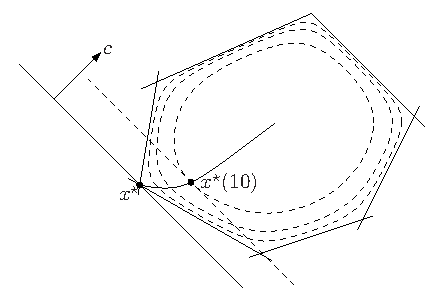
\includegraphics[width=.6\textwidth]{figures/ch11-02.pdf}
\caption*{图11.2 一个 $n=2$、$m=6$ 的 LP 的中心路径。虚线是对数障碍函数 $\phi$ 的三条等高线。随着 $t\to\infty$，中心路径收敛到最优点 $x^\star$。图中还标出了 $t=10$ 对应的中心路径上的点。在该点可以从几何上验证最优性条件 (11.9)：直线 $c^\T x=c^\T x^\star(10)$ 与经过 $x^\star(10)$ 的 $\phi$ 的等高线相切。}
\end{figure}
可见，当 $\lambda=\lambda^\star(t)$、$\nu=\nu^\star(t)$ 时，$x^\star(t)$ 最小化拉格朗日函数
\[
L(x,\lambda,\nu)=f_0(x)+\sum_{i=1}^m\lambda_i f_i(x)+\nu^\T(Ax-b),
\]
这说明 $\lambda^\star(t),\nu^\star(t)$ 是对偶可行点对。因此，对偶函数 $g(\lambda^\star(t),\nu^\star(t))$ 有限，且
\begin{align*}
g(\lambda^\star(t),\nu^\star(t))
&=f_0(x^\star(t))+\sum_{i=1}^m\lambda_i^\star(t)f_i(x^\star(t))
+\nu^\star(t)^\T(Ax^\star(t)-b)\\
&=f_0(x^\star(t))-m/t.
\end{align*}
特别地，$x^\star(t)$ 与对偶可行点对 $\lambda^\star(t),\nu^\star(t)$ 对应的对偶间隙就是 $m/t$。一个重要推论是
\[
f_0(x^\star(t))-p^\star\le m/t,
\]
即 $x^\star(t)$ 的次优程度不超过 $m/t$。这证实了如下直观认识：当 $t\to\infty$ 时，$x^\star(t)$ 收敛到一个最优点。

\begin{origexample}{11.2}
\emph{不等式形式的线性规划。} 不等式形式 LP (11.8) 的对偶为
\[
\begin{aligned}
\text{最大化}\quad&-b^\T\lambda\\
\text{约束为}\quad&A^\T\lambda+c=0,\\&\lambda\succeq0.
\end{aligned}
\]
从最优性条件 (11.9) 显然可见，
\[
\lambda_i^\star(t)=\frac1{t(b_i-a_i^\T x^\star(t))},\quad i=1,\ldots,m,
\]
% Source PDF page 581 (printed p. 567)
是对偶可行的，其对偶目标值为
\[
-b^\T\lambda^\star(t)=c^\T x^\star(t)+(Ax^\star(t)-b)^\T\lambda^\star(t)
=c^\T x^\star(t)-m/t.
\]
\end{origexample}

\subsubsection*{用 KKT 条件解释}
还可以把中心路径条件 (11.7) 看作 KKT 最优性条件 (11.2) 的连续变形。点 $x$ 等于 $x^\star(t)$ 当且仅当存在 $\lambda,\nu$ 使得
\begin{equation}\begin{aligned}
Ax&=b,\qquad f_i(x)\le0,\quad i=1,\ldots,m,\\
\lambda&\succeq0,\\
\nabla f_0(x)+\sum_{i=1}^m\lambda_i\nabla f_i(x)+A^\T\nu&=0,\\
-\lambda_i f_i(x)&=1/t,\quad i=1,\ldots,m.
\end{aligned}\tag{11.11}\end{equation}
KKT 条件 (11.2) 与中心性条件 (11.11) 的唯一区别，是将互补条件 $-\lambda_i f_i(x)=0$ 替换为 $-\lambda_i f_i(x)=1/t$。特别地，当 $t$ 很大时，$x^\star(t)$ 以及相应的对偶点 $\lambda^\star(t),\nu^\star(t)$ “几乎”满足 (11.1) 的 KKT 最优性条件。

\subsubsection*{力场解释}
可以用作用在严格可行集 $C$ 内一个质点上的势力，对中心路径作简单的力学解释。为简便起见，假设没有等式约束。

对每个约束，令它在质点位于 $x$ 时施加的力为
\[
F_i(x)=-\nabla(-\log(-f_i(x)))=\frac1{f_i(x)}\nabla f_i(x).
\]
所有约束产生的总力场对应的势为对数障碍 $\phi$。当质点向可行集边界移动时，会受到约束产生的强烈排斥力。

现在设质点在位置 $x$ 还受到另一个力
\[
F_0(x)=-t\nabla f_0(x).
\]
这个目标力场沿负梯度方向牵引质点，也就是使它向较小的 $f_0$ 移动。参数 $t$ 决定目标力相对于约束力的大小。

中心点 $x^\star(t)$ 就是约束力与质点所受目标力恰好平衡的位置。随着参数 $t$ 增大，质点被更强地牵向最优点，但它始终被障碍势限制在 $C$ 内，因为当质点接近边界时，障碍势变为无穷大。

\begin{origexample}{11.3}
\emph{不等式形式 LP 的力场解释。} 与 LP (11.8) 第 $i$ 个约束对应的力场为
\[
F_i(x)=\frac{-a_i}{b_i-a_i^\T x}.
\]
% Source PDF page 582 (printed p. 568)
\begin{figure}[htbp]\centering
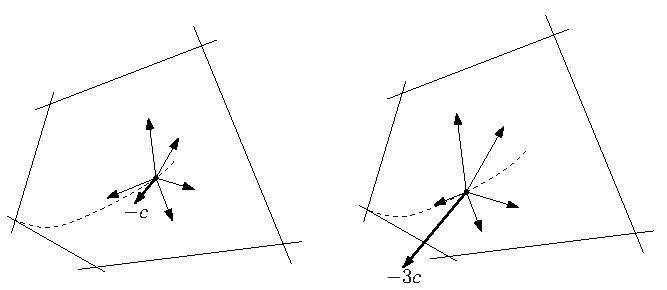
\includegraphics[width=.85\textwidth]{figures/ch11-03.pdf}
\caption*{图11.3 中心路径的力场解释。虚线表示中心路径。左右两图的圆点分别为 $x^\star(1)$ 与 $x^\star(3)$。粗箭头表示目标力，分别等于 $-c$ 与 $-3c$。其余箭头表示服从距离倒数定律的约束力。随着目标力强度变化，质点的平衡位置描出中心路径。}
\end{figure}
该力沿约束平面 $H_i=\{x\mid a_i^\T x=b_i\}$ 指向内部的法向方向，其大小与到 $H_i$ 的距离成反比，即
\[
\norm{F_i(x)}_2=\frac{\norm{a_i}_2}{b_i-a_i^\T x}=\frac1{\dist(x,H_i)}.
\]
换言之，每个约束超平面都对应一个排斥力，其大小为到该超平面距离的倒数。

项 $tc^\T x$ 是作用在质点上的常力 $-tc$ 对应的势。这个“目标力”把质点推向低成本方向。因此，$x^\star(t)$ 是质点同时受到距离倒数约束力和目标力 $-tc$ 时的平衡位置。当 $t$ 很大时，质点被推到几乎最优的位置。很强的目标力由反向的约束力平衡，而后者很大是因为质点已接近可行边界。

图11.3用一个 $n=2$、$m=5$ 的小型 LP 展示了这一解释。左图给出 $t=1$ 时的 $x^\star(t)$ 及作用其上的约束力，它们与目标力平衡。右图给出 $t=3$ 时的 $x^\star(t)$ 及相应各力。更大的目标力使质点更靠近最优点。
\end{origexample}

\section{障碍法}
% Source PDF page 582 (printed p. 568), section 11.3 begins here.
我们已经看到，点 $x^\star(t)$ 的次优程度为 $m/t$，对偶可行点对 $\lambda^\star(t),\nu^\star(t)$ 为这一精度提供了证书。由此得到一种非常直接的方法，可以按指定精度 $\epsilon$ 求解原问题 (11.1)：取 $t=m/\epsilon$，并用牛顿法求解等式约束问题
% Source PDF page 583 (printed p. 569)
\[
\begin{aligned}
\text{最小化}\quad&(m/\epsilon)f_0(x)+\phi(x)\\
\text{约束为}\quad&Ax=b.
\end{aligned}
\]
这种方法可以称为无约束最小化法，因为它通过求解一个无约束或线性约束问题，就能按保证的精度求解不等式约束问题 (11.1)。尽管对于小问题、好的初始点和中等精度（即 $\epsilon$ 不太小），这种方法能够很好地工作，但在其他情况下效果不好。因此，它极少被采用，甚至从未被采用。

\subsection{障碍法}
对无约束最小化法作一个简单扩展，就能得到效果很好的方法。它依次求解一系列无约束（或线性约束）最小化问题，以上一次找到的点作为下一个无约束最小化问题的初始点。换言之，对一系列递增的 $t$ 值计算 $x^\star(t)$，直至 $t\ge m/\epsilon$，从而保证得到原问题的一个 $\epsilon$ 次优解。Fiacco 和 McCormick 在20世纪60年代首次提出这种方法时，将其称为序列无约束最小化技术（SUMT）。现在通常称为\emph{障碍法}或\emph{路径跟踪法}。它的一个简单版本如下。

\begin{origalgorithm}{11.1}
\textbf{障碍法。}

给定严格可行点 $x$，$t:=t^{(0)}>0$，$\mu>1$，容差 $\epsilon>0$。

重复：
\begin{enumerate}
\item \textbf{中心化步骤。} 以 $x$ 为起点，在 $Ax=b$ 约束下最小化 $tf_0+\phi$，计算 $x^\star(t)$。
\item \textbf{更新。} $x:=x^\star(t)$。
\item \textbf{停止准则。} 若 $m/t<\epsilon$，退出。
\item \textbf{增大 $t$。} $t:=\mu t$。
\end{enumerate}
\end{origalgorithm}
除第一次迭代外，每次迭代均以前一次计算的中心点为起点，计算中心点 $x^\star(t)$，随后将 $t$ 乘以因子 $\mu>1$。算法还可返回 $\lambda=\lambda^\star(t)$、$\nu=\nu^\star(t)$，即一个对偶 $\epsilon$ 次优点，也就是 $x$ 的证书。

每执行一次第1步，称为一次\emph{中心化步骤}（因为在计算中心点）或\emph{外迭代}；第一次中心化步骤，即计算 $x^\star(t^{(0)})$，称为\emph{初始中心化步骤}。（因此，取 $t^{(0)}=m/\epsilon$ 的简单算法只有初始中心化步骤。）第1步可以使用任意线性约束最小化方法，但我们将假设使用牛顿法。中心化步骤中的牛顿迭代或牛顿步称为\emph{内迭代}。每个内迭代步均有一个原始可行点；但只有在每次外迭代（中心化）结束时，才有对偶可行点。

% Source PDF page 584 (printed p. 570)
\subsubsection*{中心化的精度}
对中心化问题的求解精度，有几点需要说明。没有必要精确计算 $x^\star(t)$，因为中心路径本身的意义只在于：当 $t\to\infty$ 时，它引向原问题的解；非精确中心化仍会产生收敛到最优点的点列 $x^{(k)}$。然而，非精确中心化意味着由 (11.10) 计算出的 $\lambda^\star(t),\nu^\star(t)$ 并非精确对偶可行。可以给公式 (11.10) 加一个修正项来解决这个问题：只要计算出的 $x$ 接近中心路径，即接近 $x^\star(t)$，便能得到对偶可行点（见习题11.9）。另一方面，与计算 $tf_0+\phi$ 的一个较好最小化点相比，计算一个极高精度最小化点的额外成本很少，至多增加几个牛顿步。因此，假设精确中心化并非不合理。

\subsubsection*{$\mu$ 的选择}
参数 $\mu$ 的选择涉及内迭代次数和外迭代次数之间的权衡。当 $\mu$ 很小（即接近 $1$）时，每次外迭代只将 $t$ 增大一个较小倍数。因此，牛顿过程的初始点，也就是前一个迭代点 $x$，是很好的起点，计算下一迭代点所需的牛顿步很少。于是，小 $\mu$ 对应每次外迭代较少的牛顿步，但由于每次外迭代只把间隙减小很少，外迭代次数就会很多。这种情况下，迭代点（实际上也包括内迭代的迭代点）会紧贴中心路径，这也解释了“路径跟踪法”这个名称。

当 $\mu$ 很大时，情况相反。每次外迭代后 $t$ 大幅增加，当前迭代点通常不再是下一迭代点的良好近似，所以内迭代次数会多得多。这样“激进”地更新 $t$，会减少外迭代次数，因为每次外迭代都使对偶间隙缩小 $\mu$ 倍，但会增加内迭代次数。$\mu$ 很大时，中心路径上的迭代点相距很远，内迭代点会大幅偏离中心路径。

实践与理论都证实了选择 $\mu$ 时的这一权衡。在实践中，小 $\mu$（接近 $1$）导致很多次外迭代，每次仅有几个牛顿步。在相当宽的范围内，例如 $\mu$ 从约 $3$ 到约 $100$，这两种效应几乎相抵，总牛顿步数近似不变。这说明 $\mu$ 的选择并不特别关键，约 $10$ 至 $20$ 的值似乎效果不错。当按最好的最坏情况总牛顿步数上界来选择 $\mu$ 时，则采用接近 $1$ 的值。

\subsubsection*{$t^{(0)}$ 的选择}
另一个重要问题是 $t$ 初值的选择。这里的权衡很简单：若 $t^{(0)}$ 太大，第一次外迭代需要过多内迭代；若 $t^{(0)}$ 太小，算法需要额外的外迭代，第一次中心化中也可能有过多内迭代。

由于 $m/t^{(0)}$ 是初始中心化结束时得到的对偶间隙，
% Source PDF page 585 (printed p. 571)
一个合理选择是使 $m/t^{(0)}$ 大约与 $f_0(x^{(0)})-p^\star$ 同阶，或是它的 $\mu$ 倍。例如，若已知一个对偶可行点 $\lambda,\nu$，其对偶间隙为 $\eta=f_0(x^{(0)})-g(\lambda,\nu)$，则可取 $t^{(0)}=m/\eta$。这样，第一次外迭代只是计算一个点对，其对偶间隙与初始原始、对偶可行点的间隙相同。

中心路径条件 (11.7) 还提示了另一种可能。把
\begin{equation}
\inf_\nu\norm{t\nabla f_0(x^{(0)})+\nabla\phi(x^{(0)})+A^\T\nu}_2\tag{11.12}
\end{equation}
解释为 $x^{(0)}$ 偏离 $x^\star(t)$ 的程度，并将使 (11.12) 最小的 $t$ 值作为 $t^{(0)}$。（这个 $t$ 和 $\nu$ 可以通过求解最小二乘问题得到。）

这一方法的一个变体，是用 $x$ 与 $x^\star(t)$ 之间仿射不变的偏离度量代替欧氏范数。选择使下式最小的 $t$ 和 $\nu$：
\begin{align*}
\alpha(t,\nu)={}&\bigl(t\nabla f_0(x^{(0)})+\nabla\phi(x^{(0)})+A^\T\nu\bigr)^\T H_0^{-1}\\
&\qquad\bigl(t\nabla f_0(x^{(0)})+\nabla\phi(x^{(0)})+A^\T\nu\bigr),
\end{align*}
其中
\[
H_0=t\nabla^2 f_0(x^{(0)})+\nabla^2\phi(x^{(0)}).
\]
（可以证明，$\inf_\nu\alpha(t,\nu)$ 是 $tf_0+\phi$ 在 $x^{(0)}$ 处的牛顿减量的平方。）由于 $\alpha$ 是关于 $\nu$ 和 $t$ 的二次除以线性函数，它为凸函数。

\subsubsection*{不可行初始点牛顿法}
障碍法的一种变体使用不可行初始点牛顿法（见第10.3节）完成中心化。因此，障碍法的初始点 $x^{(0)}$ 满足 $x^{(0)}\in\dom f_0$，且 $f_i(x^{(0)})<0$，$i=1,\ldots,m$，但不一定满足 $Ax^{(0)}=b$。假设问题严格可行，则第一次中心化中某一步会接受完整牛顿步，此后所有迭代点均原始可行，算法与标准障碍法一致。

\subsection{例子}
\subsubsection*{不等式形式的线性规划}
第一个例子是一个小型不等式形式 LP，
\[
\begin{aligned}\text{最小化}\quad&c^\T x\\\text{约束为}\quad&Ax\preceq b,\end{aligned}
\]
其中 $A\in\R^{100\times50}$。随机生成数据，使问题严格原始可行、严格对偶可行，而且最优值 $p^\star=1$。

初始点 $x^{(0)}$ 在中心路径上，对偶间隙为 $100$。用障碍法求解，对偶间隙小于 $10^{-6}$ 时终止。用带回溯的牛顿法求解中心化问题，参数为 $\alpha=0.01$、$\beta=0.5$。
% Source PDF page 586 (printed p. 572)
牛顿法的停止准则为 $\lambda(x)^2/2\le10^{-5}$，其中 $\lambda(x)$ 是函数 $tc^\T x+\phi(x)$ 的牛顿减量。

\begin{figure}[htbp]\centering
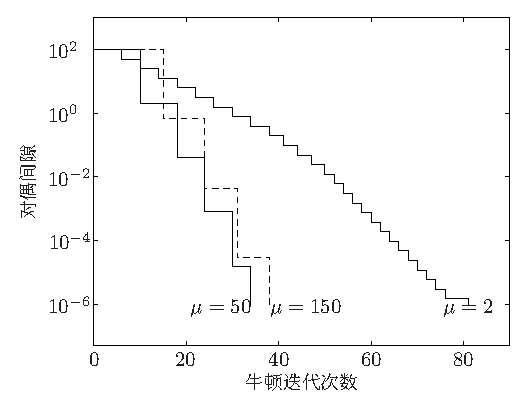
\includegraphics[width=.65\textwidth]{figures/ch11-04.pdf}
\caption*{图11.4 小型 LP 的障碍法求解过程：对偶间隙与累计牛顿步数的关系。三条曲线分别对应参数 $\mu=2,50,150$。各情况下，对偶间隙都近似线性收敛。}
\end{figure}
图11.4展示了三个参数 $\mu$ 值对应的障碍法进展。纵轴以对数尺度表示对偶间隙，横轴为累计内迭代次数，即牛顿步数，这是计算工作量的自然度量。每条曲线呈阶梯形，每个台阶对应一次外迭代。每段水平阶面的宽度，就是该次外迭代所需的牛顿步数。每段竖直阶面的高度恰好对应因子 $\mu$，因为每次外迭代结束时，对偶间隙都缩小 $\mu$ 倍。

这些曲线展示了障碍法的几个典型特征。首先，该方法效果很好，对偶间隙近似线性收敛。这是因为，对每个 $\mu$ 值，重新中心化所需的牛顿步数近似不变。$\mu=50$ 和 $\mu=150$ 时，障碍法求解该问题的总牛顿步数在 $35$ 至 $40$ 之间。

图11.4清楚地显示出 $\mu$ 选择中的权衡。$\mu=2$ 时，阶面较短，重新中心化约需 $2$ 或 $3$ 个牛顿步；但竖直阶面也短，因为每次外迭代只把对偶间隙缩小 $2$ 倍。另一个极端是 $\mu=150$，水平阶面较长，通常约需 $7$ 个牛顿步，但竖直阶面也大得多，因为每次外迭代都使对偶间隙缩小 $150$ 倍。

图11.5进一步考察选择 $\mu$ 的权衡。取 $1.2$ 至 $200$ 之间的 $25$ 个 $\mu$ 值，用障碍法求解该 LP，当对偶间隙小于 $10^{-3}$ 时终止。图中绘出了求解所需总牛顿步数随参数 $\mu$ 的变化。
% Source PDF page 587 (printed p. 573)
\begin{figure}[htbp]\centering
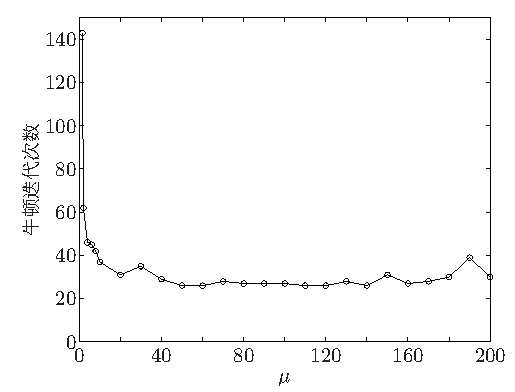
\includegraphics[width=.65\textwidth]{figures/ch11-05.pdf}
\caption*{图11.5 小型 LP 中参数 $\mu$ 的选择权衡。纵轴为将对偶间隙从 $100$ 减小到 $10^{-3}$ 所需的总牛顿步数，横轴为 $\mu$。图中可见，$\mu$ 大于约 $3$ 时障碍法效果很好，而对 $\mu$ 的具体数值并不敏感。}
\end{figure}
从图中可见，当 $\mu$ 处于约 $3$ 至 $200$ 的宽范围内时，障碍法表现都很好。正如直观所预期，$\mu$ 过小时，需要更多次外迭代，总牛顿步数因而上升。一个有意思的观察是，$\mu$ 大于约 $3$ 时，总牛顿步数变化不大。因此，当 $\mu$ 在这个范围内增大时，外迭代次数减少，恰好被每次外迭代所需牛顿步数的增加抵消。$\mu$ 进一步增大时，障碍法的性能变得较难预测，即更依赖具体问题实例。由于增大 $\mu$ 不再改善性能，选择 $10$ 至 $100$ 范围内的值比较合适。

\subsubsection*{几何规划}
考虑凸形式的几何规划，
\[
\begin{aligned}
\text{最小化}\quad&\log\left(\sum_{k=1}^{K_0}\exp(a_{0k}^\T x+b_{0k})\right)\\
\text{约束为}\quad&\log\left(\sum_{k=1}^{K_i}\exp(a_{ik}^\T x+b_{ik})\right)\le0,\quad i=1,\ldots,m,
\end{aligned}
\]
变量为 $x\in\R^n$，相应的对数障碍为
\[
\phi(x)=-\sum_{i=1}^m\log\left(-\log\sum_{k=1}^{K_i}\exp(a_{ik}^\T x+b_{ik})\right).
\]
所考察的实例有 $n=50$ 个变量和 $m=100$ 个不等式，与上面的小型 LP 相同。目标函数和各个约束函数都包含
% Source PDF page 588 (printed p. 574)
$K_i=5$ 项。随机生成这个实例，使其严格原始可行、严格对偶可行，而且最优值为 $1$。

\begin{figure}[htbp]\centering
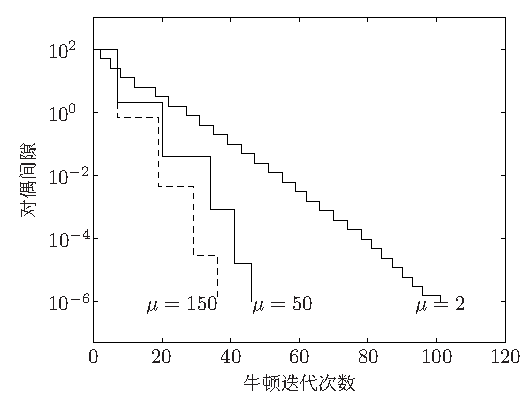
\includegraphics[width=.65\textwidth]{figures/ch11-06.pdf}
\caption*{图11.6 小型 GP 的障碍法求解过程：对偶间隙与累计牛顿步数的关系。这里同样可见对偶间隙近似线性收敛。}
\end{figure}
初始点 $x^{(0)}$ 位于中心路径上，对偶间隙为 $100$。分别取 $\mu=2$、$\mu=50$、$\mu=150$，用障碍法求解，当对偶间隙小于 $10^{-6}$ 时终止。中心化问题用牛顿法求解，参数与 LP 例子相同，即 $\alpha=0.01$、$\beta=0.5$，停止准则为 $\lambda(x)^2/2\le10^{-5}$。

图11.6给出了对偶间隙随累计牛顿步数的变化，它与图11.4中的 LP 曲线非常相似。特别地，每次中心化所需的牛顿步数近似不变，因此对偶间隙近似线性收敛。

求解所需总牛顿步数随参数 $\mu$ 的变化，也与 LP 例子十分相似。对于这个 GP，$\mu$ 在 $10$ 至 $200$ 之间时，将对偶间隙减小到 $10^{-3}$ 以下约需 $30$ 个牛顿步，实际范围约为 $20$ 至 $40$。所以这里选择 $10$ 至 $100$ 范围内的 $\mu$ 也比较合适。

\subsubsection*{一族标准形式 LP}
在上面的例子中，我们对维数相近的随机 LP 和 GP 实例，考察了障碍法进展，即对偶间隙随累计牛顿步数的变化。两者的结果非常相似，都显示出对偶间隙随牛顿步数近似线性收敛。还考察了性能随参数 $\mu$ 的变化，两个例子的结果也基本相同。$\mu$ 大于约 $10$ 时，障碍法效果很好，约需 $30$ 个牛顿步就能将对偶间隙从 $10^2$ 减小到 $10^{-6}$。
% Source PDF page 589 (printed p. 575)
在两种情况下，只要 $\mu$ 大于约 $10$，其选择几乎不影响所需的总牛顿步数。

本节考察障碍法性能随问题维数的变化。考虑标准形式 LP
\[
\begin{aligned}
\text{最小化}\quad&c^\T x\\\text{约束为}\quad&Ax=b,\qquad x\succeq0,
\end{aligned}
\]
其中 $A\in\R^{m\times n}$。对一族随机生成的实例，研究所需总牛顿步数与变量数 $n$、等式约束数 $m$ 的关系。取 $n=2m$，即变量数为约束数的两倍。

问题按如下方式生成。$A$ 的元素独立同分布，服从均值为零、方差为一的正态分布 $\mathcal N(0,1)$。取 $b=Ax^{(0)}$，其中 $x^{(0)}$ 各分量独立，均匀分布在 $[0,1]$ 上。这保证问题严格原始可行，因为 $x^{(0)}\succ0$ 且可行。构造成本向量 $c$ 时，先计算向量 $z\in\R^m$ 和 $s\in\R^n$，前者各分量服从 $\mathcal N(0,1)$，后者各分量均匀分布在 $[0,1]$ 上，然后取 $c=A^\T z+s$。这保证问题严格对偶可行，因为 $A^\T z\prec c$。

算法参数取 $\mu=100$，中心化步骤的参数与前面例子相同：回溯参数 $\alpha=0.01$、$\beta=0.5$，停止准则 $\lambda(x)^2/2\le10^{-5}$。初始点在中心路径上，$t^{(0)}=1$，即间隙为 $n$。将初始对偶间隙缩小 $10^4$ 倍，也就是完成两次外迭代后终止算法。

图11.7给出了 $m=50$、$m=500$、$m=1000$ 三个实例的对偶间隙与迭代次数的关系。曲线与前面各图非常相似，对偶间隙近似线性收敛。问题规模从 $50$ 个约束（$100$ 个变量）增大到 $1000$ 个约束（$2000$ 个变量）时，所需牛顿步数只略有增加。

为考察问题规模对牛顿步数的影响，在 $m=10$ 至 $m=1000$ 之间取 $20$ 个值，每个值生成 $100$ 个实例。用障碍法求解这 $2000$ 个问题，记录所需牛顿步数。图11.8汇总了结果，对每个 $m$ 给出牛顿步数的均值与标准差。首先，标准差约为 $2$ 次迭代，且似乎近似独立于问题规模。由于所需平均步数约为 $25$，这意味着所需牛顿步数的变化仅约为 $\pm10\%$。

图中显示，问题维数扩大 $100$ 倍时，所需牛顿步数仅从约 $21$ 略增到约 $27$。这也是障碍法一般具有的典型表现：所需牛顿步数随维数增长很慢，几乎总是几十步。当然，执行一个牛顿步的计算工作量会随问题维数增大。
% Source PDF page 590 (printed p. 576)
\begin{figure}[htbp]\centering
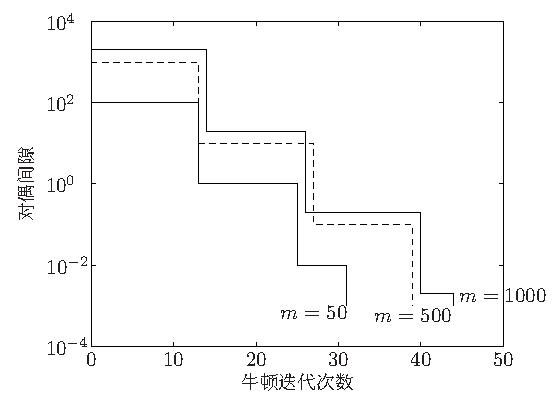
\includegraphics[width=.67\textwidth]{figures/ch11-07.pdf}
\caption*{图11.7 三个不同维数的随机标准形式 LP 的障碍法进展：对偶间隙与累计牛顿步数的关系。各问题变量数为 $n=2m$。这里同样可见对偶间隙近似线性收敛，而较大问题所需的牛顿步数略有增加。}
\end{figure}
\begin{figure}[htbp]\centering
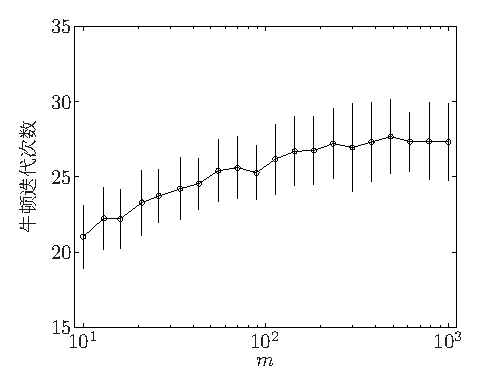
\includegraphics[width=.6\textwidth]{figures/ch11-08.pdf}
\caption*{图11.8 不同维数下求解 $100$ 个随机 LP 所需的平均牛顿步数，$n=2m$。误差棒给出每个 $m$ 值下围绕均值的标准差。问题维数变化 $100$ 倍时，所需牛顿步数的增长很小。}
\end{figure}

% Source PDF page 591 (printed p. 577)
\subsection{收敛性分析}
障碍法的收敛性分析很直接。假设对 $t=t^{(0)},\mu t^{(0)},\mu^2t^{(0)},\ldots$，都能用牛顿法最小化 $tf_0+\phi$，则完成初始中心化以及另外 $k$ 次中心化之后，对偶间隙为 $m/(\mu^k t^{(0)})$。因此，达到要求的精度 $\epsilon$，恰好需要初始中心化，再加上
\begin{equation}
\left\lceil\frac{\log(m/(\epsilon t^{(0)}))}{\log\mu}\right\rceil\tag{11.13}
\end{equation}
次中心化。

因此，只要在 $t\ge t^{(0)}$ 时可以用牛顿法求解中心化问题 (11.6)，障碍法就有效。对于标准牛顿法，一个充分条件是：对 $t\ge t^{(0)}$，函数 $tf_0+\phi$ 满足第10.2.4节（第529页）的条件，即初始下水平集为闭集，相应 KKT 矩阵的逆有界，而且 Hessian 矩阵满足 Lipschitz 条件。（第11.5节将详细讨论基于自协调性的另一组充分条件。）若中心化采用不可行初始点牛顿法，则第10.3.3节（第536页）列出的条件足以保证收敛。

假设 $f_0,\ldots,f_m$ 为闭函数，对原问题作简单修改就能保证这些条件成立。在问题中增加约束 $\norm{x}_2^2\le R^2$，可推出对每个 $t\ge0$，$tf_0+\phi$ 都强凸，特别地，中心化步骤中的牛顿法保证收敛（见习题11.4）。

这一分析说明，在合理假设下障碍法确实收敛，但没有回答一个基本问题：随着参数 $t$ 增大，中心化问题是否越来越难，因而需要越来越多次迭代？数值证据表明，对许多不同类型的问题，情况并非如此：即使 $t$ 增大，中心化问题所需的牛顿步数似乎也近似不变。第11.5节将看到，对于满足某些自协调条件的问题，可以解决这个问题。

\subsection{修改后的 KKT 方程的牛顿步}
在障碍法中，牛顿步 $\Delta x_{\mathrm{nt}}$ 及相应对偶变量由下列线性方程给出：
\begin{equation}
\begin{bmatrix}t\nabla^2 f_0(x)+\nabla^2\phi(x)&A^\T\\A&0\end{bmatrix}
\begin{bmatrix}\Delta x_{\mathrm{nt}}\\\nu_{\mathrm{nt}}\end{bmatrix}
=-\begin{bmatrix}t\nabla f_0(x)+\nabla\phi(x)\\0\end{bmatrix}.\tag{11.14}
\end{equation}
本节说明，中心化问题的这些牛顿步可以解释为以一种特定方式直接求解修改后 KKT 方程
\begin{equation}\begin{aligned}
\nabla f_0(x)+\sum_{i=1}^m\lambda_i\nabla f_i(x)+A^\T\nu&=0,\\
-\lambda_i f_i(x)&=1/t,\quad i=1,\ldots,m,\\
Ax&=b
\end{aligned}\tag{11.15}\end{equation}
时得到的牛顿步。

% Source PDF page 592 (printed p. 578)
修改后的 KKT 方程 (11.15) 是关于 $n+p+m$ 个变量 $x,\nu,\lambda$ 的 $n+p+m$ 个非线性方程。求解时，首先用 $\lambda_i=-1/(tf_i(x))$ 消去变量 $\lambda_i$，得到
\begin{equation}
\nabla f_0(x)+\sum_{i=1}^m\frac1{-tf_i(x)}\nabla f_i(x)+A^\T\nu=0,
\qquad Ax=b,\tag{11.16}
\end{equation}
这是关于 $n+p$ 个变量 $x,\nu$ 的 $n+p$ 个方程。

为求解非线性方程组 (11.16) 的牛顿步，对第一个方程中的非线性项作 Taylor 近似。$v$ 很小时有
\begin{align*}
&\nabla f_0(x+v)+\sum_{i=1}^m\frac1{-tf_i(x+v)}\nabla f_i(x+v)\\
&\quad\approx\nabla f_0(x)+\sum_{i=1}^m\frac1{-tf_i(x)}\nabla f_i(x)+\nabla^2 f_0(x)v\\
&\qquad+\sum_{i=1}^m\frac1{-tf_i(x)}\nabla^2 f_i(x)v
+\sum_{i=1}^m\frac1{tf_i(x)^2}\nabla f_i(x)\nabla f_i(x)^\T v.
\end{align*}
用这个 Taylor 近似替换方程 (11.16) 中的非线性项，就得到牛顿步对应的线性方程
\begin{equation}
Hv+A^\T\nu=-g,\qquad Av=0,\tag{11.17}
\end{equation}
其中
\begin{align*}
H&=\nabla^2 f_0(x)+\sum_{i=1}^m\frac1{-tf_i(x)}\nabla^2 f_i(x)
+\sum_{i=1}^m\frac1{tf_i(x)^2}\nabla f_i(x)\nabla f_i(x)^\T,\\
g&=\nabla f_0(x)+\sum_{i=1}^m\frac1{-tf_i(x)}\nabla f_i(x).
\end{align*}
注意到
\[
H=\nabla^2 f_0(x)+(1/t)\nabla^2\phi(x),\qquad
g=\nabla f_0(x)+(1/t)\nabla\phi(x),
\]
因此由 (11.14)，障碍法中心化步骤的牛顿步 $\Delta x_{\mathrm{nt}}$ 与 $\nu_{\mathrm{nt}}$ 满足
\[
tH\Delta x_{\mathrm{nt}}+A^\T\nu_{\mathrm{nt}}=-tg,\qquad A\Delta x_{\mathrm{nt}}=0.
\]
与 (11.17) 比较可得
\[
v=\Delta x_{\mathrm{nt}},\qquad\nu=(1/t)\nu_{\mathrm{nt}}.
\]
这说明，对偶变量经过缩放后，中心化问题 (11.6) 的牛顿步可以解释为求解修改后 KKT 方程 (11.16) 的牛顿步。

这种方法先从修改后的 KKT 方程中消去变量 $\lambda$，再应用牛顿法求解得到的方程组。另一种变体不预先消去 $\lambda$，而是直接对修改后的 KKT 方程应用牛顿法。这样就得到第11.7节讨论的原始—对偶搜索方向。

% Source PDF page 593 (printed p. 579)
\section{可行性与第一阶段方法}
障碍法需要严格可行初始点 $x^{(0)}$。如果不知道这样的点，则先进行一个称为\emph{第一阶段}的预备过程，计算严格可行点，或确定约束不可行。然后将第一阶段得到的严格可行点作为障碍法的初始点，此时的障碍法称为\emph{第二阶段}。本节介绍几种第一阶段方法。

\subsection{基本的第一阶段方法}
考虑关于变量 $x\in\R^n$ 的一组不等式与等式
\begin{equation}
f_i(x)\le0,\quad i=1,\ldots,m,\qquad Ax=b,\tag{11.18}
\end{equation}
其中 $f_i:\R^n\to\R$ 为凸函数，具有连续的二阶导数。假设已给定点 $x^{(0)}\in\dom f_1\cap\cdots\cap\dom f_m$，满足 $Ax^{(0)}=b$。

我们的目标是找到严格满足这些不等式与等式的解，或判定不存在这样的解。为此构造优化问题
\begin{equation}\begin{aligned}
\text{最小化}\quad&s\\
\text{约束为}\quad&f_i(x)\le s,\quad i=1,\ldots,m,\\
&Ax=b,
\end{aligned}\tag{11.19}\end{equation}
变量为 $x\in\R^n$、$s\in\R$。变量 $s$ 可解释为不等式最大违反程度的上界；目标是将最大违反程度降到零以下。

这个问题总是严格可行，因为可以选 $x^{(0)}$ 作为 $x$ 的初始点，并选任意大于 $\max_{i=1,\ldots,m}f_i(x^{(0)})$ 的数作为 $s$。因此，可以应用障碍法求解 (11.19)，它称为不等式与等式系统 (11.19) 对应的第一阶段优化问题。

根据 (11.19) 最优值 $\bar p^\star$ 的正负，可以分为三种情况。
\begin{enumerate}
\item 若 $\bar p^\star<0$，则 (11.18) 有严格可行解。而且，若 $(x,s)$ 对 (11.19) 可行且 $s<0$，则 $x$ 满足 $f_i(x)<0$。这意味着不必高精度求解优化问题 (11.19)，在 $s<0$ 时即可终止。
\item 若 $\bar p^\star>0$，则 (11.18) 不可行。与情况1一样，无须高精度求解第一阶段优化问题 (11.19)：找到对偶目标为正的对偶可行点时即可终止，因为这证明 $\bar p^\star>0$。此时可以根据对偶可行点，构造证明 (11.18) 不可行的择一系统的解。
\item 若 $\bar p^\star=0$，且最小值在 $x^\star$、$s^\star=0$ 处取得，则该不等式组可行，但不严格可行。若 $\bar p^\star=0$，但最小值未取得，则不等式组不可行。
% Source PDF page 594 (printed p. 580)
实际中不可能精确判定 $\bar p^\star=0$。应用于 (11.19) 的优化算法会以 $|\bar p^\star|<\epsilon$ 的结论终止，其中 $\epsilon$ 是某个很小的正数。这使我们能够断定，不等式组 $f_i(x)\le-\epsilon$ 不可行，而不等式组 $f_i(x)\le\epsilon$ 可行。
\end{enumerate}

\subsubsection*{违反程度之和}
刚介绍的基本第一阶段方法有许多变体。一种方法最小化违反程度之和，而非最大违反程度。构造问题
\begin{equation}\begin{aligned}
\text{最小化}\quad&\one^\T s\\
\text{约束为}\quad&f_i(x)\le s_i,\quad i=1,\ldots,m,\\
&Ax=b,\\&s\succeq0.
\end{aligned}\tag{11.20}\end{equation}
固定 $x$ 时，$s_i$ 的最优值为 $\max\{f_i(x),0\}$，所以这个问题是在最小化违反程度之和。(11.20) 的最优值为零且能取得，当且仅当原来的等式与不等式组可行。

当等式与不等式系统 (11.19) 不可行时，这个违反程度之和第一阶段方法有一个很有意思的性质。第一阶段问题 (11.20) 的最优点通常只违反很少的几个不等式，设为 $r$ 个。因此，我们计算出了一个满足很多（$m-r$ 个）不等式的点，也就是识别出一个很大的可行不等式子集。此时，严格满足的不等式对应的对偶变量为零，因而还证明了某个不等式子集不可行。这比只知道全部 $m$ 个不等式合在一起不可行，提供了更多信息。（这一现象与寻找稀疏近似解时采用的 $\ell_1$ 范数正则化或基追踪密切相关；见第6.1.2节和第6.5.4节。）

\begin{origexample}{11.4}
\emph{第一阶段方法的比较。} 对一个不可行不等式组 $Ax\preceq b$ 应用两种第一阶段方法，维数为 $m=100$、$n=50$。第一种是基本第一阶段方法
\[
\begin{aligned}\text{最小化}\quad&s\\\text{约束为}\quad&Ax\preceq b+\one s,\end{aligned}
\]
它最小化最大违反程度。第二种最小化违反程度之和，即求解 LP
\[
\begin{aligned}\text{最小化}\quad&\one^\T s\\\text{约束为}\quad&Ax\preceq b+s,\\&s\succeq0.\end{aligned}
\]
这两种方法求得的 $x$ 分别记为 $x_{\mathrm{max}}$、$x_{\mathrm{sum}}$。图11.9给出了两者的违反程度 $b_i-a_i^\T x$ 的分布。点 $x_{\mathrm{max}}$ 满足 $100$ 个不等式中的 $39$ 个，而 $x_{\mathrm{sum}}$ 满足其中 $79$ 个。
\end{origexample}

% Source PDF page 595 (printed p. 581)
\begin{figure}[htbp]\centering
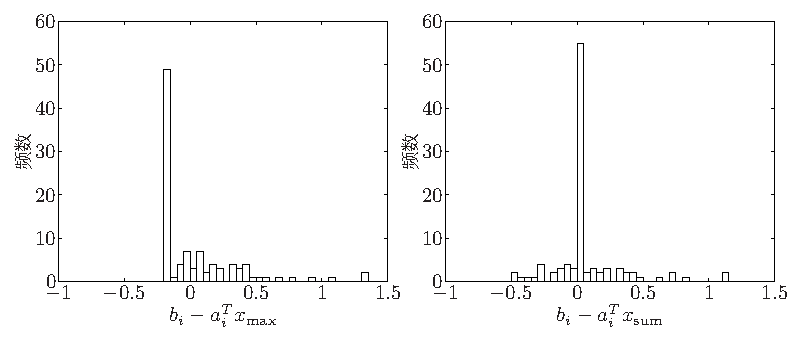
\includegraphics[width=.95\textwidth]{figures/ch11-09.pdf}
\caption*{图11.9 一个含 $100$ 个不等式 $a_i^\T x\le b_i$、$50$ 个变量的不可行不等式组，其违反程度 $b_i-a_i^\T x$ 的分布。左图的 $x_{\mathrm{max}}$ 由基本第一阶段算法得到，它满足 $100$ 个不等式中的 $39$ 个。右图的 $x_{\mathrm{sum}}$ 通过最小化违反程度之和得到，它满足 $100$ 个不等式中的 $79$ 个。}
\end{figure}
\subsubsection*{在第二阶段中心路径附近终止}
使用障碍法的基本第一阶段方法有一个简单变体，具有如下性质：当等式与不等式组严格可行时，第一阶段问题的中心路径与原优化问题 (11.1) 的中心路径相交。

假设给定点 $x^{(0)}\in\mathcal D=\dom f_0\cap\dom f_1\cap\cdots\cap\dom f_m$，且 $Ax^{(0)}=b$。构造第一阶段优化问题
\begin{equation}\begin{aligned}
\text{最小化}\quad&s\\
\text{约束为}\quad&f_i(x)\le s,\quad i=1,\ldots,m,\\
&f_0(x)\le M,\\&Ax=b,
\end{aligned}\tag{11.21}\end{equation}
其中常数 $M$ 取为大于 $\max\{f_0(x^{(0)}),p^\star\}$。

现在假设原问题 (11.1) 严格可行，于是 (11.21) 的最优值 $\bar p^\star$ 为负。问题 (11.21) 的中心路径由下列条件刻画：
\[
\sum_{i=1}^m\frac1{s-f_i(x)}=\bar t,\qquad
\frac{\nabla f_0(x)}{M-f_0(x)}+\sum_{i=1}^m\frac{\nabla f_i(x)}{s-f_i(x)}+A^\T\nu=0,
\]
其中 $\bar t$ 为参数。若 $(x,s)$ 在中心路径上且 $s=0$，则 $x$ 和 $\nu$ 满足
\[
t\nabla f_0(x)+\sum_{i=1}^m\frac1{-f_i(x)}\nabla f_i(x)+A^\T\nu=0,
\]
其中 $t=1/(M-f_0(x))$。这说明 $x$ 在原优化问题 (11.1) 的中心路径上，
% Source PDF page 596 (printed p. 582)
对应的对偶间隙为
\begin{equation}
m(M-f_0(x))\le m(M-p^\star).\tag{11.22}
\end{equation}

\subsection{用不可行初始点牛顿法实现第一阶段}
也可以对原问题的一个修改版本应用不可行初始点牛顿法，完成第一阶段。原问题为
\[
\begin{aligned}\text{最小化}\quad&f_0(x)\\\text{约束为}\quad&f_i(x)\le0,\quad i=1,\ldots,m,\\&Ax=b.\end{aligned}
\]
首先将问题写成显然等价的形式
\[
\begin{aligned}\text{最小化}\quad&f_0(x)\\\text{约束为}\quad&f_i(x)\le s,\quad i=1,\ldots,m,\\&Ax=b,\qquad s=0,\end{aligned}
\]
其中增加了变量 $s\in\R$。为启动障碍法，用不可行初始点牛顿法求解
\[
\begin{aligned}
\text{最小化}\quad&t^{(0)}f_0(x)-\sum_{i=1}^m\log(s-f_i(x))\\
\text{约束为}\quad&Ax=b,\qquad s=0.
\end{aligned}
\]
可用任意 $x\in\mathcal D$ 以及任意 $s>\max_i f_i(x)$ 初始化。只要问题严格可行，不可行初始点牛顿法最终会采用一个无阻尼步，此后有 $s=0$，即 $x$ 严格可行。

若连这些函数公共定义域 $\mathcal D$ 内的一个点也不知道，同样可以使用这一技巧。只需对问题
\[
\begin{aligned}
\text{最小化}\quad&t^{(0)}f_0(x+z_0)-\sum_{i=1}^m\log(s-f_i(x+z_i))\\
\text{约束为}\quad&Ax=b,\qquad s=0,\qquad z_0=0,\ \ldots,\ z_m=0,
\end{aligned}
\]
应用不可行初始点牛顿法，变量为 $x,z_0,\ldots,z_m$ 以及 $s\in\R$。初始化 $z_i$ 时使 $x+z_i\in\dom f_i$。

用这种方法处理第一阶段问题的主要缺点，是在问题不可行时没有好的停止准则；残差只是无法收敛到零。

\subsection{例子}
考虑一族线性可行性问题
\[
Ax\preceq b(\gamma),
\]
其中 $A\in\R^{50\times20}$，$b(\gamma)=b+\gamma\Delta b$。选取数据，使不等式组在 $\gamma>0$ 时严格可行，$\gamma<0$ 时不可行，$\gamma=0$ 时可行但不严格可行。

% Source PDF page 597 (printed p. 583)
图11.10给出 $\gamma$ 在 $[-1,1]$ 内取 $40$ 个值时，找到严格可行点或不可行证书所需的总牛顿步数。使用第11.4.1节的基本第一阶段方法，即对每个 $\gamma$ 构造 LP
\[
\begin{aligned}\text{最小化}\quad&s\\\text{约束为}\quad&Ax\preceq b(\gamma)+s\one.\end{aligned}
\]
障碍法参数取 $\mu=10$，初始点为 $x=0$、$s=-\min_i b_i(\gamma)+1$。找到满足 $s<0$ 的点 $(x,s)$，或找到对偶问题
\[
\begin{aligned}
\text{最大化}\quad&-b(\gamma)^\T z\\
\text{约束为}\quad&A^\T z=0,\\&\one^\T z=1,\\&z\succeq0
\end{aligned}
\]
的可行解 $z$ 且 $-b(\gamma)^\T z>0$ 时，算法终止。

图中显示，若不等式组具有一定可行余量，约需 $25$ 个牛顿步就能找到严格可行点。反之，若不等式组具有一定不可行余量，则约需 $35$ 步得到证明不可行的证书。当不等式组接近可行与不可行的分界，即 $\gamma$ 接近零时，第一阶段的计算工作量增大。当 $\gamma$ 非常接近零，即不等式组非常接近可行与不可行的分界时，所需步数显著增长。图11.11给出 $\gamma$ 接近零时的总牛顿步数。曲线表明，对于非常接近可行与不可行分界的问题，检测可行性或证明不可行性所需步数近似按对数增长。

这个例子具有代表性：只要问题不十分接近可行与不可行的分界，用障碍法求解凸不等式组与线性等式组的成本就不大，而且近似不变。当问题非常接近分界时，寻找严格可行点或不可行证书所需的牛顿步数增加。当问题恰好位于严格可行与不可行之间的边界上，例如可行但不严格可行时，成本变为无穷大。

\subsubsection*{用不可行初始点牛顿法求可行点}
还对问题
\[
\begin{aligned}\text{最小化}\quad&-\sum_{i=1}^m\log s_i\\\text{约束为}\quad&Ax+s=b(\gamma)\end{aligned}
\]
应用不可行初始点牛顿法，求解同一组可行性问题。

采用回溯参数 $\alpha=0.01$、$\beta=0.9$，初始化 $x^{(0)}=0$、$s^{(0)}=\one$、$\nu^{(0)}=0$。只考察可行问题，即 $\gamma>0$，并在找到可行点时终止。（不考察不可行问题，因为这种情况下残差只会收敛到一个正数。）图11.12给出找到可行点所需牛顿步数随 $\gamma$ 的变化。

% Source PDF page 598 (printed p. 584)
\begin{figure}[htbp]\centering
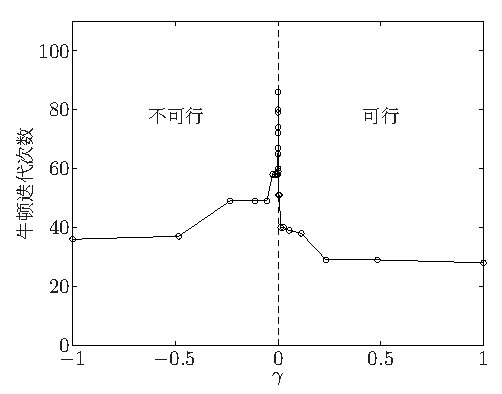
\includegraphics[width=.63\textwidth]{figures/ch11-10.pdf}
\caption*{图11.10 判定由 $\gamma\in\R$ 参数化的线性不等式组 $Ax\preceq b+\gamma\Delta b$ 可行或不可行所需的牛顿迭代次数。不等式组在 $\gamma>0$ 时严格可行，在 $\gamma<0$ 时不可行。$\gamma$ 大于约 $0.2$ 时，计算严格可行点约需 $30$ 步；$\gamma$ 小于约 $-0.5$ 时，产生不可行证书约需 $35$ 步。中间的 $\gamma$ 值，特别是接近零时，需要更多牛顿步才能判定可行性。}
\end{figure}
\begin{figure}[htbp]\centering
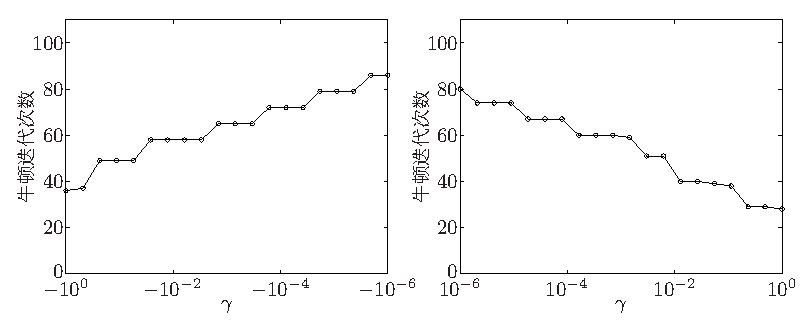
\includegraphics[width=.95\textwidth]{figures/ch11-11.pdf}
\caption*{图11.11 左：$\gamma$ 为很小负数时，找到不可行性证明所需的牛顿迭代次数与 $\gamma$ 的关系。右：$\gamma$ 为很小正数时，找到严格可行点所需的牛顿迭代次数与 $\gamma$ 的关系。}
\end{figure}

% Source PDF page 599 (printed p. 585), conclusion of section 11.4.3.
\begin{figure}[htbp]\centering
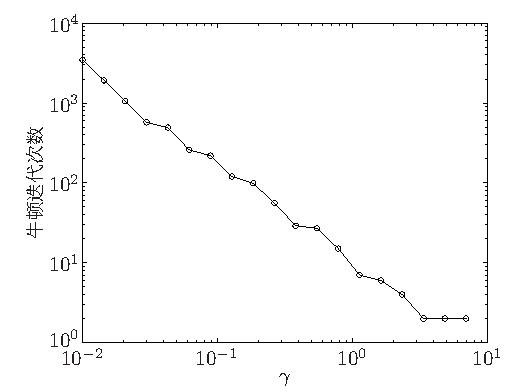
\includegraphics[width=.65\textwidth]{figures/ch11-12.pdf}
\caption*{图11.12 对由 $\gamma\in\R$ 参数化的线性不等式组 $Ax\preceq b+\gamma\Delta b$，找到可行点所需的迭代次数。使用不可行初始点牛顿法，在找到可行点时终止。$\gamma=10$ 时，初始点 $x^{(0)}=0$ 恰好可行，因此无需迭代。}
\end{figure}
图中可见，$\gamma$ 大于约 $0.3$ 时，找到可行点所需的牛顿步数少于 $20$。这些情况下，该方法比总共约需 $30$ 个牛顿步的第一阶段方法更有效。$\gamma$ 更小时，所需牛顿步数急剧增加，近似与 $1/\gamma$ 成正比。$\gamma=0.01$ 时，不可行初始点牛顿法需要几千次迭代才能得到可行点。在这个范围内，第一阶段方法有效得多，仅需约 $40$ 次迭代。

这些结果很有代表性。只要不等式组可行，而且不很接近可行与不可行的分界，不可行初始点牛顿法就效果很好。但当可行集只是勉强非空时，例如本例中 $\gamma$ 很小的情况，第一阶段方法好得多。第一阶段方法的另一个优点，是能妥善处理不可行情形；相比之下，不可行初始点牛顿法只会不收敛。


% Source PDF page 599 (printed p. 585), section 11.5 begins here.
\section{基于自协调性的复杂度分析}
利用自协调函数的牛顿法复杂度分析（第9.6.4节，第503页；第10.2.4节，第531页），可以分析障碍法的复杂度。这种分析适用于许多常见问题，并得到几个有意思的结论：它严格给出用障碍法求解问题所需总牛顿步数的上界，并说明为何中心化问题不会随着 $t$ 增大而变得更困难。

% Source PDF page 600 (printed p. 586)
\subsection{自协调性假设}
作以下两个假设。
\begin{itemize}
\item 对所有 $t\ge t^{(0)}$，函数 $tf_0+\phi$ 为闭函数且自协调。
\item 问题 (11.1) 的下水平集有界。
\end{itemize}
第二个假设说明中心化问题的下水平集有界（见习题11.3），因此中心化问题可解。下水平集有界还意味着 $tf_0+\phi$ 的 Hessian 矩阵处处正定（见习题11.14）。虽然自协调性假设将复杂度分析限制在一类特定问题上，但应当强调，无论这一假设是否成立，障碍法一般都能很好地工作。

许多问题满足自协调性假设，包括所有线性问题和二次问题。若函数 $f_i$ 为线性或二次函数，则
\[
tf_0-\sum_{i=1}^m\log(-f_i)
\]
对所有 $t\ge0$ 都自协调（见第9.6节）。因此下面的复杂度分析适用于 LP、QP 和 QCQP。

有时可以重新表述问题，使其满足自协调性假设。例如，考虑线性不等式约束熵最大化问题
\[
\begin{aligned}
\text{最小化}\quad&\sum_{i=1}^n x_i\log x_i\\
\text{约束为}\quad&Fx\preceq g,\\&Ax=b.
\end{aligned}
\]
函数
\[
tf_0(x)+\phi(x)=t\sum_{i=1}^n x_i\log x_i-\sum_{i=1}^m\log(g_i-\bar f_i^\T x),
\]
其中 $\bar f_1^\T,\ldots,\bar f_m^\T$ 是 $F$ 的各行，它不是闭函数（除非 $Fx\preceq g$ 蕴含 $x\succeq0$），也不自协调。但可以增加冗余不等式约束 $x\succeq0$，得到等价问题
\begin{equation}\begin{aligned}
\text{最小化}\quad&\sum_{i=1}^n x_i\log x_i\\
\text{约束为}\quad&Fx\preceq g,\\&Ax=b,\\&x\succeq0.
\end{aligned}\tag{11.23}\end{equation}
此时有
\[
tf_0(x)+\phi(x)=t\sum_{i=1}^n x_i\log x_i-\sum_{i=1}^n\log x_i-\sum_{i=1}^m\log(g_i-\bar f_i^\T x),
\]
% Source PDF page 601 (printed p. 587)
对任意 $t\ge0$，它都是自协调闭函数。（对所有 $t\ge0$，函数 $ty\log y-\log y$ 在 $\R_{++}$ 上自协调；见习题11.13。）因此，复杂度分析适用于重新表述后的线性不等式约束熵最大化问题 (11.23)。

再看一个更特殊的例子，考虑 GP
\[
\begin{aligned}
\text{最小化}\quad&f_0(x)=\log\sum_{k=1}^{K_0}\exp(a_{0k}^\T x+b_{0k})\\
\text{约束为}\quad&\log\sum_{k=1}^{K_i}\exp(a_{ik}^\T x+b_{ik})\le0,\quad i=1,\ldots,m.
\end{aligned}
\]
尚不清楚函数
\begin{align*}
tf_0(x)+\phi(x)={}&t\log\left(\sum_{k=1}^{K_0}\exp(a_{0k}^\T x+b_{0k})\right)\\
&-\sum_{i=1}^m\log\left(-\log\sum_{k=1}^{K_i}\exp(a_{ik}^\T x+b_{ik})\right)
\end{align*}
是否自协调，因此，尽管障碍法有效，本节的复杂度分析却不一定成立。

不过，可以把 GP 重新表述为明确满足自协调性假设的形式。对每一项（单项式）$\exp(a_{ik}^\T x+b_{ik})$，引入新变量 $y_{ik}$ 作为上界：
\[
\exp(a_{ik}^\T x+b_{ik})\le y_{ik}.
\]
用这些新变量，可将 GP 写为
\[
\begin{aligned}
\text{最小化}\quad&\sum_{k=1}^{K_0}y_{0k}\\
\text{约束为}\quad&\sum_{k=1}^{K_i}y_{ik}\le1,\quad i=1,\ldots,m,\\
&a_{ik}^\T x+b_{ik}-\log y_{ik}\le0,\quad i=0,\ldots,m,\quad k=1,\ldots,K_i,\\
&y_{ik}\ge0,\quad i=0,\ldots,m,\quad k=1,\ldots,K_i.
\end{aligned}
\]
对应的对数障碍为
\[
\sum_{i=0}^m\sum_{k=1}^{K_i}\bigl(-\log y_{ik}-\log(\log y_{ik}-a_{ik}^\T x-b_{ik})\bigr)
-\sum_{i=1}^m\log\left(1-\sum_{k=1}^{K_i}y_{ik}\right),
\]
它是自协调闭函数（例9.8，第500页）。由于目标为线性函数，对任意 $t$，$tf_0+\phi$ 都是自协调闭函数。

\subsection{每次中心化的牛顿迭代次数}
第9.6.4节（第503页）和第10.2.4节（第531页）中建立的自协调函数牛顿法复杂度理论表明，最小化严格凸、自协调闭函数 $f$ 所需的牛顿迭代次数，上界为
\begin{equation}
\frac{f(x)-p^\star}{\gamma}+c.\tag{11.24}
\end{equation}
% Source PDF page 602 (printed p. 588)
其中 $x$ 是牛顿法的初始点，$p^\star=\inf_x f(x)$ 是最优值。常数 $\gamma$ 只依赖回溯参数 $\alpha$ 和 $\beta$，由下式给出：
\[
\frac1\gamma=\frac{20-8\alpha}{\alpha\beta(1-2\alpha)^2}.
\]
常数 $c$ 只依赖容差 $\epsilon_{\mathrm{nt}}$，
\[
c=\log_2\log_2(1/\epsilon_{\mathrm{nt}}),
\]
可以合理地用 $c=6$ 近似。式 (11.24) 是一个相当保守的牛顿步数上界，但本节只关心建立复杂度界，重点考察它怎样随问题规模与算法参数增长。

本节用这一结果推导障碍法一次外迭代所需的牛顿步数界，也就是从 $x^\star(t)$ 出发计算 $x^\star(\mu t)$ 的步数界。为简化记号，用 $x$ 表示当前迭代点 $x^\star(t)$，用 $x^+$ 表示下一个迭代点 $x^\star(\mu t)$，用 $\lambda$、$\nu$ 分别表示 $\lambda^\star(t)$、$\nu^\star(t)$。

自协调性假设说明，
\begin{equation}
\frac{\mu t f_0(x)+\phi(x)-\mu t f_0(x^+)-\phi(x^+)}{\gamma}+c\tag{11.25}
\end{equation}
是从 $x=x^\star(t)$ 出发计算 $x^+=x^\star(\mu t)$ 所需牛顿步数的上界。遗憾的是，在实际算出 $x^+$，即执行牛顿算法之前，不知道 $x^+$，也就不知道上界 (11.25)；而执行之后，已经知道计算 $x^\star(\mu t)$ 所需的准确步数，这就失去了求上界的意义。但可以如下推导 (11.25) 的上界：
\begin{align*}
&\mu t f_0(x)+\phi(x)-\mu t f_0(x^+)-\phi(x^+)\\
&=\mu t f_0(x)-\mu t f_0(x^+)+\sum_{i=1}^m\log(-\mu t\lambda_i f_i(x^+))-m\log\mu\\
&\le\mu t f_0(x)-\mu t f_0(x^+)-\mu t\sum_{i=1}^m\lambda_i f_i(x^+)-m-m\log\mu\\
&=\mu t f_0(x)-\mu t\left(f_0(x^+)+\sum_{i=1}^m\lambda_i f_i(x^+)+\nu^\T(Ax^+-b)\right)-m-m\log\mu\\
&\le\mu t f_0(x)-\mu t g(\lambda,\nu)-m-m\log\mu\\
&=m(\mu-1-\log\mu).
\end{align*}
这串等式与不等式需要解释。从第一行到第二行，使用了 $\lambda_i=-1/(tf_i(x))$。第一个不等式使用 $a>0$ 时 $\log a\le a-1$。从第三行到第四行，使用 $Ax^+=b$，因此增加的项 $\nu^\T(Ax^+-b)$ 为零。第二个不等式来自
% Source PDF page 603 (printed p. 589)
对偶函数的定义：
\begin{align*}
g(\lambda,\nu)&=\inf_z\left(f_0(z)+\sum_{i=1}^m\lambda_i f_i(z)+\nu^\T(Az-b)\right)\\
&\le f_0(x^+)+\sum_{i=1}^m\lambda_i f_i(x^+)+\nu^\T(Ax^+-b).
\end{align*}
最后一行来自 $g(\lambda,\nu)=f_0(x)-m/t$。

\begin{figure}[htbp]\centering
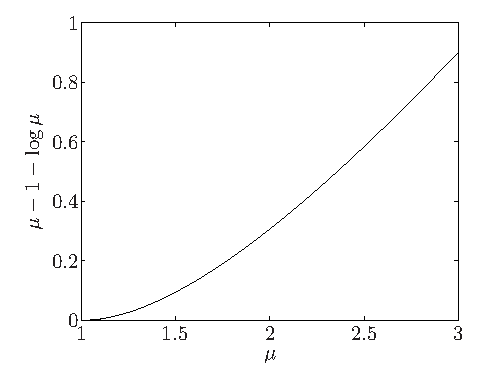
\includegraphics[width=.6\textwidth]{figures/ch11-13.pdf}
\caption*{图11.13 函数 $\mu-1-\log\mu$ 随 $\mu$ 的变化。障碍法一次外迭代所需牛顿步数的上界为 $(m/\gamma)(\mu-1-\log\mu)+c$。}
\end{figure}
结论是
\begin{equation}
\frac{m(\mu-1-\log\mu)}{\gamma}+c\tag{11.26}
\end{equation}
是 (11.25) 的上界，因此也是障碍法一次外迭代所需牛顿步数的上界。图11.13给出函数 $\mu-1-\log\mu$。$\mu$ 较小时，它近似二次增长；$\mu$ 很大时，它近似线性增长。这符合我们的直观：$\mu$ 接近 $1$ 时，中心化所需牛顿步数较少；$\mu$ 很大时，步数完全可能增加。

界 (11.26) 表明，每次中心化所需的牛顿步数，有一个主要取决于 $\mu$ 和 $m$ 的上界，其中 $\mu$ 是障碍法每次外迭代更新 $t$ 的倍数，$m$ 是问题的不等式约束数。它还弱依赖内迭代线搜索的参数 $\alpha$ 和 $\beta$，并以很弱的方式依赖内迭代的终止容差。有意思的是，这个界不依赖变量维数 $n$、等式约束数 $p$，也不依赖问题数据，即目标函数和约束函数的具体取值，前提是第11.5.1节的自协调性假设成立。最后，它不依赖 $t$；特别地，当 $t\to\infty$ 时，每次外迭代的牛顿步数仍有一致上界。

% Source PDF page 604 (printed p. 590)
\subsection{总牛顿迭代次数}
现在可以给出障碍法总牛顿步数的上界，不计初始中心化，后者将在第一阶段分析中讨论。将每次外迭代的牛顿步数上界 (11.26) 与外迭代次数 (11.13) 相乘，得到所需总牛顿步数的上界
\begin{equation}
N=\left\lceil\frac{\log(m/(t^{(0)}\epsilon))}{\log\mu}\right\rceil
\left(\frac{m(\mu-1-\log\mu)}{\gamma}+c\right).\tag{11.27}
\end{equation}
这一公式表明，自协调性假设成立时，对任意 $\mu>1$，都能界定障碍法所需的牛顿步数。

固定 $\mu$ 和 $m$ 时，上界 $N$ 与 $\log(m/(t^{(0)}\epsilon))$ 成正比。后者是初始对偶间隙 $m/t^{(0)}$ 与最终对偶间隙 $\epsilon$ 的比值的对数，即要求的对偶间隙缩减倍数的对数。因此可以说障碍法至少线性收敛，因为达到给定精度所需的步数，随精度倒数按对数增长。

固定 $\mu$ 与要求的对偶间隙缩减倍数时，上界 $N$ 随不等式数 $m$ 线性增长。它不依赖其他维数 $n,p$ 以及具体的问题数据或函数。下面将看到，按依赖 $m$ 的特定方式选择 $\mu$，可以使牛顿步数的上界仅按 $\sqrt m$，而不是按 $m$ 增长。

最后，考察上界 $N$ 随算法参数 $\mu$ 的变化。当 $\mu$ 趋近 $1$ 时，$N$ 中的第一项变大，因此 $N$ 变大。这与直观和观察相符：$\mu$ 接近 $1$ 时，外迭代次数很大。$\mu$ 很大时，上界 $N$ 近似按 $\mu/\log\mu$ 增长，这次是因为每次外迭代所需牛顿步数的上界增大。这同样与观察一致。因此，$N$ 作为 $\mu$ 的函数有最小值。

图11.14展示了上界随参数 $\mu$ 的变化，绘出了以下数值下 (11.27) 与 $\mu$ 的关系：
\[
c=6,\qquad\gamma=1/375,\qquad m/(t^{(0)}\epsilon)=10^5,\qquad m=100.
\]
该界在定性上符合直观和观察：$\mu$ 趋近 $1$ 时很大，$\mu$ 很大时则较慢地增大。$N$ 在 $\mu\approx1.02$ 处取最小值，此时总牛顿迭代次数的上界约为 $8000$。牛顿法的复杂度分析保守，但图中反映了选择 $\mu$ 的基本权衡。（实际中，大得多的 $\mu$，例如约 $2$ 至 $100$，都效果很好，总牛顿迭代次数只是几十次。）

\subsubsection*{将 $\mu$ 选为 $m$ 的函数}
固定 $\mu$ 及要求的对偶间隙缩减倍数时，界 (11.27) 随不等式数 $m$ 线性增长。将 $\mu$ 选为 $m$ 的函数，可以改善 $m$ 的幂指数。取
% Source PDF page 605 (printed p. 591)
\begin{equation}
\mu=1+1/\sqrt m.\tag{11.28}
\end{equation}
\begin{figure}[htbp]\centering
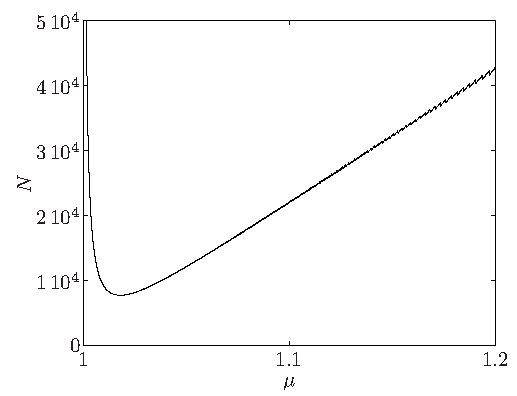
\includegraphics[width=.64\textwidth]{figures/ch11-14.pdf}
\caption*{图11.14 式 (11.27) 给出的总牛顿迭代次数上界 $N$ 与障碍算法参数 $\mu$ 的关系，其中 $c=6$、$\gamma=1/375$、$m=100$，对偶间隙缩减倍数 $m/(t^{(0)}\epsilon)=10^5$。}
\end{figure}
则 (11.27) 中的第二项满足
\begin{align*}
\mu-1-\log\mu&=1/\sqrt m-\log(1+1/\sqrt m)\\
&\le1/\sqrt m-1/\sqrt m+1/(2m)\\
&=1/(2m),
\end{align*}
这里使用 $a\ge0$ 时 $-\log(1+a)\le-a+a^2/2$。由对数的凹性，还有
\[
\log\mu=\log(1+1/\sqrt m)\ge(\log2)/\sqrt m.
\]
利用这些不等式，总牛顿步数的界为
\begin{equation}\begin{aligned}
N&\le\left\lceil\frac{\log(m/(t^{(0)}\epsilon))}{\log\mu}\right\rceil
\left(\frac{m(\mu-1-\log\mu)}\gamma+c\right)\\
&\le\left\lceil\frac{\sqrt m\log(m/(t^{(0)}\epsilon))}{\log2}\right\rceil
\left(\frac1{2\gamma}+c\right)\\
&=\left\lceil\sqrt m\log_2(m/(t^{(0)}\epsilon))\right\rceil
\left(\frac1{2\gamma}+c\right)\\
&\le c_1+c_2\sqrt m,
\end{aligned}\tag{11.29}\end{equation}
其中
\[
c_1=\frac1{2\gamma}+c,\qquad
c_2=\log_2(m/(t^{(0)}\epsilon))\left(\frac1{2\gamma}+c\right).
\]
% Source PDF page 606 (printed p. 592)
这里 $c_1$ 只弱依赖中心化牛顿步骤的算法参数，$c_2$ 还依赖要求的对偶间隙缩减倍数。注意，$\log_2(m/(t^{(0)}\epsilon))$ 正好是要求缩减对偶间隙的比特数。

固定对偶间隙缩减倍数时，界 (11.29) 按 $\sqrt m$ 增长，而若固定参数 $\mu$，(11.27) 中的上界 $N$ 按 $m$ 增长。因此，参数取 (11.28) 的障碍法称为 $\sqrt m$ 阶方法。

实际中不会采用 $\mu=1+1/\sqrt m$，因为这个值太小，甚至不会将 $\mu$ 选为随 $m$ 减小的函数。我们之所以关注这个 $\mu$，只是因为它近似最小化了那个非常保守的牛顿步数上界，并给出按 $\sqrt m$ 而非 $m$ 增长的总估计。

\subsection{可行性问题}
本节分析第11.4.1节基本第一阶段方法的一个小变体的复杂度，用它求解凸不等式组
\begin{equation}
f_1(x)\le0,\quad\ldots,\quad f_m(x)\le0,\tag{11.30}
\end{equation}
其中 $f_1,\ldots,f_m$ 为凸函数，具有连续的二阶导数。（等式约束留到后面考虑。）假设第一阶段问题
\begin{equation}\begin{aligned}
\text{最小化}\quad&s\\\text{约束为}\quad&f_i(x)\le s,\quad i=1,\ldots,m
\end{aligned}\tag{11.31}\end{equation}
满足第11.5.1节的条件。特别地，假设不等式组 (11.30) 的可行集（它当然可以为空）包含在半径为 $R$ 的欧氏球内：
\[
\{x\mid f_i(x)\le0,\ i=1,\ldots,m\}\subseteq\{x\mid\norm{x}_2\le R\}.
\]
可将 $R$ 解释为不等式组中任一可行点范数的先验界。这一假设意味着第一阶段问题的下水平集有界。不失一般性，以 $x=0$ 作为第一阶段方法的起点。定义 $F=\max_i f_i(0)$ 为最大约束违反程度，假设它为正，否则 $x=0$ 已满足 (11.30)。

用 $\bar p^\star$ 表示第一阶段优化问题 (11.31) 的最优值。$\bar p^\star$ 的符号决定不等式组 (11.30) 是否可行，其大小也有意义。如果 $\bar p^\star$ 为正且很大，例如接近它可能达到的最大值 $F$，则不等式组相当不可行：对每个 $x$，至少有一个不等式被明显违反，违反程度至少为 $\bar p^\star$。另一方面，若 $\bar p^\star$ 为负且绝对值很大，则不等式组相当可行：不仅存在 $x$ 使所有 $f_i(x)$ 非正，而且存在 $x$ 使所有 $f_i(x)$ 都是相当大的负数，不超过 $\bar p^\star$。因此，$|\bar p^\star|$ 衡量不等式组的可行性或不可行性有多明确，进而与
% Source PDF page 607 (printed p. 593)
判定 (11.30) 可行性的难度有关。特别地，若 $|\bar p^\star|$ 很小，意味着问题接近可行与不可行的分界。

为判定不等式组的可行性，采用基本第一阶段问题 (11.31) 的一个变体，增加冗余线性不等式 $a^\T x\le1$，得到
\begin{equation}\begin{aligned}
\text{最小化}\quad&s\\\text{约束为}\quad&f_i(x)\le s,\quad i=1,\ldots,m,\\&a^\T x\le1.
\end{aligned}\tag{11.32}\end{equation}
稍后给出 $a$。所选的 $a$ 将满足 $\norm{a}_2\le1/R$，于是 $\norm{x}_2\le R$ 蕴含 $a^\T x\le1$，即附加约束冗余。

选择 $a$ 和 $s_0$，使 $x=0$、$s=s_0$ 位于问题 (11.32) 的中心路径上，对应参数值 $t^{(0)}$，即它们最小化
\[
t^{(0)}s-\sum_{i=1}^m\log(s-f_i(x))-\log(1-a^\T x).
\]
令关于 $s$ 的导数为零，得到
\begin{equation}
t^{(0)}=\sum_{i=1}^m\frac1{s_0-f_i(0)}.\tag{11.33}
\end{equation}
令关于 $x$ 的梯度为零，得到
\begin{equation}
a=-\sum_{i=1}^m\frac1{s_0-f_i(0)}\nabla f_i(0).\tag{11.34}
\end{equation}
因此只剩参数 $s_0$ 尚需选择。选定后，向量 $a$ 由 (11.34) 给出，参数 $t^{(0)}$ 由 (11.33) 给出。由于 $x=0$、$s=s_0$ 必须对第一阶段问题 (11.32) 严格可行，必须取 $s_0>F$。

还必须选择 $s_0$，保证 $\norm{a}_2\le1/R$。由 (11.34)，
\[
\norm{a}_2\le\sum_{i=1}^m\frac1{s_0-f_i(0)}\norm{\nabla f_i(0)}_2\le\frac{mG}{s_0-F},
\]
其中 $G=\max_i\norm{\nabla f_i(0)}_2$。因此可取 $s_0=mGR+F$，使 $\norm{a}_2\le1/R$，从而附加线性不等式冗余。

利用 (11.33)，有
\[
t^{(0)}=\sum_{i=1}^m\frac1{mGR+F-f_i(0)}\ge\frac1{mGR},
\]
因为 $F=\max_i f_i(0)$。于是 $x=0$、$s=s_0$ 位于第一阶段问题 (11.32) 的中心路径上，其初始对偶间隙满足
\[
\frac{m+1}{t^{(0)}}\le(m+1)mGR.
\]

% Source PDF page 608 (printed p. 594)
为求解原不等式组 (11.30)，需要判定 $\bar p^\star$ 的符号。当 (11.32) 的原始目标值为负，或对偶目标值为正时即可停止。当 (11.32) 的对偶间隙小于 $|\bar p^\star|$ 时，必然出现这两种情况之一。

用障碍法求解 (11.32)，从对偶间隙不超过 $(m+1)mGR$ 的中心点出发，在对偶间隙小于 $|\bar p^\star|$ 时或之前终止。利用前一节的结果，所需牛顿步数不超过
\begin{equation}
\left\lceil\sqrt{m+1}\log_2\frac{m(m+1)GR}{|\bar p^\star|}\right\rceil
\left(\frac1{2\gamma}+c\right).\tag{11.35}
\end{equation}
这里取 $\mu=1+1/\sqrt{m+1}$，它比固定 $\mu$ 能给出更好的 $m$ 的复杂度指数。

界 (11.35) 的增长只略快于 $\sqrt m$，并且弱依赖中心化步骤的算法参数。它近似与 $\log_2((GR)/|\bar p^\star|)$ 成正比，可将后者解释为具体可行性问题的难度，或它距可行与不可行分界的接近程度。

\subsubsection*{含等式约束的可行性问题}
通过消去等式约束，同样的分析可用于含等式约束的可行性问题。消元不影响自协调性，但此时 $G$ 与 $R$ 指的是约化后，即消元后的问题。

\subsection{第一阶段与第二阶段的合并复杂度}
本节对使用障碍法的一个变体求解问题
\[
\begin{aligned}\text{最小化}\quad&f_0(x)\\\text{约束为}\quad&f_i(x)\le0,\quad i=1,\ldots,m,\\&Ax=b\end{aligned}
\]
给出从头到尾的复杂度分析。首先求解第一阶段问题
\[
\begin{aligned}
\text{最小化}\quad&s\\
\text{约束为}\quad&f_i(x)\le s,\quad i=1,\ldots,m,\\
&f_0(x)\le M,\\&Ax=b,\\&a^\T x\le1,
\end{aligned}
\]
假设它满足第11.5.1节的自协调性与下水平集有界假设。这里在基本第一阶段问题中加了两个冗余不等式。加入约束 $f_0(x)\le M$，是为了保证第一阶段的中心路径与第二阶段中心路径相交，正如第11.4.1节描述的那样，见 (11.21)。$M$ 是问题最优值的先验界。第二个新增约束为线性不等式 $a^\T x\le1$，其中 $a$ 按
% Source PDF page 609 (printed p. 595)
第11.5.4节选取。用障碍法求解这一问题，取 $\mu=1+1/\sqrt{m+2}$，初始点 $x=0$、$s=s_0$ 按第11.5.4节给出。

找到严格可行点或确定问题不可行，所需牛顿步数不超过
\begin{equation}
N_{\mathrm I}=\left\lceil\sqrt{m+2}\log_2\frac{(m+1)(m+2)GR}{|\bar p^\star|}\right\rceil
\left(\frac1{2\gamma}+c\right),\tag{11.36}
\end{equation}
其中 $G$ 与 $R$ 见第11.5.4节。如果问题不可行，算法结束；如果问题可行，则在第一阶段找到与 $s=0$ 对应的点，它位于第二阶段问题
\[
\begin{aligned}
\text{最小化}\quad&f_0(x)\\
\text{约束为}\quad&f_i(x)\le0,\quad i=1,\ldots,m,\\
&Ax=b,\\&a^\T x\le1
\end{aligned}
\]
的中心路径上。该初始点对应的初始对偶间隙不超过 $(m+1)(M-p^\star)$，见 (11.22)。假设第二阶段问题也满足第11.5.1节的自协调性与下水平集有界假设。

现在进入第二阶段，仍使用障碍法。必须将对偶间隙从不超过 $(m+1)(M-p^\star)$ 的初值降低到某个容差 $\epsilon>0$，至多需要
\begin{equation}
N_{\mathrm{II}}=\left\lceil\sqrt{m+1}\log_2\frac{(m+1)(M-p^\star)}{\epsilon}\right\rceil
\left(\frac1{2\gamma}+c\right)\tag{11.37}
\end{equation}
个牛顿步。

因此总牛顿步数不超过 $N_{\mathrm I}+N_{\mathrm{II}}$。该界随不等式数 $m$ 近似按 $\sqrt m$ 增长，并包含依赖具体问题实例的两项
\[
\log_2\frac{GR}{|\bar p^\star|},\qquad\log_2\frac{M-p^\star}{\epsilon}.
\]

\subsection{小结}
本节的复杂度分析主要有理论意义。特别提醒读者，本节讨论的 $\mu=1+1/\sqrt m$ 在实际中是很差的选择；它唯一的优点，是得到按 $\sqrt m$ 而非 $m$ 增长的界。同样，实际中也不推荐增加冗余不等式 $a^\T x\le1$。

由上述分析得到的实际数值界远高于观察到的迭代次数。甚至界的阶数似乎也保守。最好的牛顿步数界按 $\sqrt m$ 增长，而实际经验表明，牛顿步数几乎不随 $m$，实际上也几乎不随任何其他参数增长。

不过，知道自协调性条件成立时，可以为障碍法每次中心化
% Source PDF page 610 (printed p. 596)
所需的牛顿步数给出一致上界，仍然让人放心。障碍法一个明显的潜在问题是：随着 $t$ 增大，对应的中心化问题可能越来越难，需要更多牛顿步。虽然实际经验表明并非如此，一致上界进一步增强了我们对其不会发生的信心。

最后指出，重新表述问题使其满足自协调性条件，是否能带来实际优势，目前尚不清楚。只能说，自协调性条件成立时，障碍法在实践中会很好地工作，而且可以给出最坏情况复杂度界。

% Source PDF page 610 (printed p. 596), section 11.6 begins here.
\section{含广义不等式的问题}
本节说明怎样将障碍法扩展到含广义不等式的问题。考虑问题
\begin{equation}\begin{aligned}
\text{最小化}\quad&f_0(x)\\
\text{约束为}\quad&f_i(x)\preceq_{K_i}0,\quad i=1,\ldots,m,\\
&Ax=b,
\end{aligned}\tag{11.38}\end{equation}
其中 $f_0:\R^n\to\R$ 为凸函数，$f_i:\R^n\to\R^{k_i}$，$i=1,\ldots,k$，为 $K_i$ 凸函数，$K_i\subseteq\R^{k_i}$ 为正常锥。与第11.1节一样，假设 $f_i$ 二阶连续可微，$A\in\R^{p\times n}$ 且 $\rank A=p$，并假设问题可解。

问题 (11.38) 的 KKT 条件为
\begin{equation}\begin{aligned}
Ax^\star&=b,\\
f_i(x^\star)&\preceq_{K_i}0,\quad i=1,\ldots,m,\\
\lambda_i^\star&\succeq_{K_i^*}0,\quad i=1,\ldots,m,\\
\nabla f_0(x^\star)+\sum_{i=1}^m Df_i(x^\star)^\T\lambda_i^\star+A^\T\nu^\star&=0,\\
(\lambda_i^\star)^\T f_i(x^\star)&=0,\quad i=1,\ldots,m,
\end{aligned}\tag{11.39}\end{equation}
其中 $Df_i(x^\star)\in\R^{k_i\times n}$ 是 $f_i$ 在 $x^\star$ 处的导数。假设问题 (11.38) 严格可行，因此 KKT 条件是 $x^\star$ 最优的充要条件。

该方法的建立与标量约束情形平行。一旦将对数函数推广到一般正常锥上，就可以定义问题 (11.38) 的对数障碍函数。此后的推导与标量情形基本相同，特别是中心路径、障碍法和复杂度分析都非常相似。

% Source PDF page 611 (printed p. 597)
\subsection{对数障碍与中心路径}
\subsubsection*{正常锥的广义对数}
首先，为正常锥 $K\subseteq\R^q$ 定义类似 $\log x$ 的函数。若 $\psi:\R^q\to\R$ 满足以下条件，就称它为 $K$ 的\emph{广义对数}。
\begin{itemize}
\item $\psi$ 为凹、闭、二阶连续可微函数，$\dom\psi=\operatorname{int}K$，且当 $y\in\operatorname{int}K$ 时，$\nabla^2\psi(y)\prec0$。
\item 存在常数 $\theta>0$，使得对所有 $y\succ_K0$ 和 $s>0$，都有
\[
\psi(sy)=\psi(y)+\theta\log s.
\]
换言之，沿锥 $K$ 内任一射线，$\psi$ 的行为都像对数。
\end{itemize}
称常数 $\theta$ 为 $\psi$ 的\emph{次数}，因为 $\exp\psi$ 是 $\theta$ 次齐次函数。注意广义对数只在相差一个加法常数的意义下定义：如果 $\psi$ 是 $K$ 的广义对数，则对 $a\in\R$，$\psi+a$ 也是。普通对数当然是 $\R_+$ 的广义对数。

将使用任意广义对数都满足的以下两个性质。若 $y\succ_K0$，则
\begin{equation}
\nabla\psi(y)\succ_{K^*}0,\tag{11.40}
\end{equation}
这说明 $\psi$ 是 $K$ 递增的（见第3.6.1节），而且
\[
y^\T\nabla\psi(y)=\theta.
\]
第一个性质在习题11.15中证明。第二个性质对 $\psi(sy)=\psi(y)+\theta\log s$ 关于 $s$ 求导即可得到。

\begin{origexample}{11.5}
\emph{非负正交锥。} 函数 $\psi(x)=\sum_{i=1}^n\log x_i$ 是 $K=\R_+^n$ 的广义对数，次数为 $n$。对 $x\succ0$，
\[
\nabla\psi(x)=(1/x_1,\ldots,1/x_n),
\]
因此 $\nabla\psi(x)\succ0$，且 $x^\T\nabla\psi(x)=n$。
\end{origexample}

\begin{origexample}{11.6}
\emph{二阶锥。} 函数
\[
\psi(x)=\log\left(x_{n+1}^2-\sum_{i=1}^n x_i^2\right)
\]
是二阶锥
\[
K=\left\{x\in\R^{n+1}\;\middle|\;\left(\sum_{i=1}^n x_i^2\right)^{1/2}\le x_{n+1}\right\}
\]
% Source PDF page 612 (printed p. 598)
的广义对数，次数为 $2$。$\psi$ 在 $x\in\operatorname{int}K$ 处的梯度为
\[
\frac{\partial\psi(x)}{\partial x_j}=\frac{-2x_j}{x_{n+1}^2-\sum_{i=1}^n x_i^2},\quad j=1,\ldots,n,
\qquad
\frac{\partial\psi(x)}{\partial x_{n+1}}=\frac{2x_{n+1}}{x_{n+1}^2-\sum_{i=1}^n x_i^2}.
\]
容易验证 $\nabla\psi(x)\in\operatorname{int}K^*=\operatorname{int}K$ 和 $x^\T\nabla\psi(x)=2$。
\end{origexample}

\begin{origexample}{11.7}
\emph{半正定锥。} 函数 $\psi(X)=\log\det X$ 是锥 $\mathbf S_+^p$ 的广义对数，次数为 $p$，因为对 $s>0$，
\[
\log\det(sX)=\log\det X+p\log s.
\]
$\psi$ 在 $X\in\mathbf S_{++}^p$ 处的梯度等于
\[
\nabla\psi(X)=X^{-1}.
\]
于是 $\nabla\psi(X)=X^{-1}\succ0$，而 $X$ 与 $\nabla\psi(X)$ 的内积等于 $\tr(XX^{-1})=p$。
\end{origexample}

\subsubsection*{广义不等式的对数障碍函数}
回到问题 (11.38)，设 $\psi_1,\ldots,\psi_m$ 分别为锥 $K_1,\ldots,K_m$ 的广义对数，次数为 $\theta_1,\ldots,\theta_m$。定义问题 (11.38) 的对数障碍函数为
\[
\phi(x)=-\sum_{i=1}^m\psi_i(-f_i(x)),\qquad
\dom\phi=\{x\mid f_i(x)\prec_{K_i}0,\ i=1,\ldots,m\}.
\]
$\phi$ 的凸性来自 $\psi_i$ 的 $K_i$ 递增性以及 $f_i$ 的 $K_i$ 凸性，见第3.6.2节的复合规则。

\subsubsection*{中心路径}
下一步定义问题 (11.38) 的中心路径。对 $t\ge0$，将中心点 $x^\star(t)$ 定义为 $tf_0+\phi$ 在 $Ax=b$ 约束下的最小化点，即问题
\[
\begin{aligned}
\text{最小化}\quad&tf_0(x)-\sum_{i=1}^m\psi_i(-f_i(x))\\
\text{约束为}\quad&Ax=b
\end{aligned}
\]
的解，假设最小化点存在且唯一。中心点由最优性条件
\begin{equation}\begin{aligned}
t\nabla f_0(x)+\nabla\phi(x)+A^\T\nu
&=t\nabla f_0(x)+\sum_{i=1}^m Df_i(x)^\T\nabla\psi_i(-f_i(x))+A^\T\nu\\
&=0
\end{aligned}\tag{11.41}\end{equation}
刻画，其中某个 $\nu\in\R^p$ 存在，$Df_i(x)$ 是 $f_i$ 在 $x$ 处的导数。

% Source PDF page 613 (printed p. 599)
\subsubsection*{中心路径上的对偶点}
与标量情形一样，中心路径上的点给出问题 (11.38) 的对偶可行点。对 $i=1,\ldots,m$，定义
\begin{equation}
\lambda_i^\star(t)=\frac1t\nabla\psi_i(-f_i(x^\star(t))),\tag{11.42}
\end{equation}
令 $\nu^\star(t)=\nu/t$，其中 $\nu$ 是 (11.41) 中的最优对偶变量。下面证明 $\lambda_1^\star(t),\ldots,\lambda_m^\star(t)$ 连同 $\nu^\star(t)$，对原问题 (11.38) 对偶可行。

首先，由广义对数的单调性 (11.40)，$\lambda_i^\star(t)\succ_{K_i^*}0$。其次，由 (11.41) 可知，拉格朗日函数
\[
L(x,\lambda^\star(t),\nu^\star(t))=f_0(x)+\sum_{i=1}^m\lambda_i^\star(t)^\T f_i(x)
+\nu^\star(t)^\T(Ax-b)
\]
在 $x=x^\star(t)$ 处取得最小值。因此，对偶函数 $g$ 在 $(\lambda^\star(t),\nu^\star(t))$ 处的值为
\begin{align*}
g(\lambda^\star(t),\nu^\star(t))
&=f_0(x^\star(t))+\sum_{i=1}^m\lambda_i^\star(t)^\T f_i(x^\star(t))
+\nu^\star(t)^\T(Ax^\star(t)-b)\\
&=f_0(x^\star(t))+(1/t)\sum_{i=1}^m\nabla\psi_i(-f_i(x^\star(t)))^\T f_i(x^\star(t))\\
&=f_0(x^\star(t))-(1/t)\sum_{i=1}^m\theta_i,
\end{align*}
其中 $\theta_i$ 为 $\psi_i$ 的次数。最后一行使用了 $y\succ_{K_i}0$ 时 $y^\T\nabla\psi_i(y)=\theta_i$，因此
\begin{equation}
\lambda_i^\star(t)^\T f_i(x^\star(t))=-\theta_i/t,\quad i=1,\ldots,m.\tag{11.43}
\end{equation}
于是定义
\[
\bar\theta=\sum_{i=1}^m\theta_i,
\]
则原始可行点 $x^\star(t)$ 与对偶可行点 $(\lambda^\star(t),\nu^\star(t))$ 的对偶间隙为 $\bar\theta/t$。这与标量情形相同，只不过不等式数 $m$ 被各锥广义对数次数之和 $\bar\theta$ 替代。

\begin{origexample}{11.8}
\emph{二阶锥规划。} 考虑变量为 $x\in\R^n$ 的 SOCP：
\begin{equation}\begin{aligned}
\text{最小化}\quad&f^\T x\\
\text{约束为}\quad&\norm{A_i x+b_i}_2\le c_i^\T x+d_i,\quad i=1,\ldots,m,
\end{aligned}\tag{11.44}\end{equation}
其中 $A_i\in\R^{n_i\times n}$。正如例11.6所示，函数
\[
\psi(y)=\log\left(y_{p+1}^2-\sum_{i=1}^p y_i^2\right)
\]
% Source PDF page 614 (printed p. 600)
是 $\R^{p+1}$ 中二阶锥的广义对数，次数为 $2$。对应于 (11.44) 的对数障碍函数为
\begin{equation}
\phi(x)=-\sum_{i=1}^m\log\bigl((c_i^\T x+d_i)^2-\norm{A_i x+b_i}_2^2\bigr),\tag{11.45}
\end{equation}
其定义域为 $\dom\phi=\{x\mid\norm{A_i x+b_i}_2<c_i^\T x+d_i,\ i=1,\ldots,m\}$。中心路径上的最优性条件为 $tf+\nabla\phi(x^\star(t))=0$，其中
\[
\nabla\phi(x)=-2\sum_{i=1}^m
\frac{(c_i^\T x+d_i)c_i-A_i^\T(A_i x+b_i)}{(c_i^\T x+d_i)^2-\norm{A_i x+b_i}_2^2}.
\]
因此，点
\[
z_i^\star(t)=\frac{-2}{t\alpha_i}(A_i x^\star(t)+b_i),\qquad
w_i^\star(t)=\frac2{t\alpha_i}(c_i^\T x^\star(t)+d_i),\quad i=1,\ldots,m,
\]
其中 $\alpha_i=(c_i^\T x^\star(t)+d_i)^2-\norm{A_i x^\star(t)+b_i}_2^2$，对对偶问题
\[
\begin{aligned}
\text{最大化}\quad&-\sum_{i=1}^m(b_i^\T z_i+d_i w_i)\\
\text{约束为}\quad&\sum_{i=1}^m(A_i^\T z_i+c_i w_i)=f,\\
&\norm{z_i}_2\le w_i,\quad i=1,\ldots,m
\end{aligned}
\]
严格可行。$x^\star(t)$ 与 $(z^\star(t),w^\star(t))$ 对应的对偶间隙为
\[
\sum_{i=1}^m\bigl((A_i x^\star(t)+b_i)^\T z_i^\star(t)
+(c_i^\T x^\star(t)+d_i)w_i^\star(t)\bigr)=\frac{2m}{t},
\]
与一般公式 $\bar\theta/t$ 一致，因为 $\theta_i=2$。
\end{origexample}

\begin{origexample}{11.9}
\emph{不等式形式的半定规划。} 考虑变量为 $x\in\R^n$ 的 SDP
\[
\begin{aligned}\text{最小化}\quad&c^\T x\\\text{约束为}\quad&F(x)=x_1F_1+\cdots+x_nF_n+G\preceq0,\end{aligned}
\]
其中 $G,F_1,\ldots,F_n\in\mathbf S^p$。其对偶问题为
\[
\begin{aligned}\text{最大化}\quad&\tr(GZ)\\\text{约束为}\quad&\tr(F_iZ)+c_i=0,\quad i=1,\ldots,n,\\&Z\succeq0.\end{aligned}
\]
使用半正定锥 $\mathbf S_+^p$ 的广义对数 $\log\det X$，得到原始问题的障碍函数
\[
\phi(x)=\log\det(-F(x)^{-1}),\qquad\dom\phi=\{x\mid F(x)\prec0\}.
\]
对严格可行的 $x$，$\phi$ 的梯度为
\[
\frac{\partial\phi(x)}{\partial x_i}=\tr(-F(x)^{-1}F_i),\quad i=1,\ldots,n,
\]
由此得到刻画中心点的最优性条件
\[
tc_i+\tr(-F(x^\star(t))^{-1}F_i)=0,\quad i=1,\ldots,n.
\]
因此矩阵
\[
Z^\star(t)=\frac1t(-F(x^\star(t)))^{-1}
\]
严格对偶可行，$x^\star(t)$ 与 $Z^\star(t)$ 对应的对偶间隙为 $p/t$。
\end{origexample}

% Source PDF page 615 (printed p. 601)
\subsection{障碍法}
我们已经看到，中心路径的关键性质可以推广到含广义不等式的问题。
\begin{itemize}
\item 计算中心路径上的一个点，就是在等式约束下最小化一个二阶可微凸函数，可用牛顿法完成。
\item 对中心点 $x^\star(t)$，可以构造一个对偶可行点 $(\lambda^\star(t),\nu^\star(t))$，对应对偶间隙为 $\bar\theta/t$。特别地，$x^\star(t)$ 的次优程度不超过 $\bar\theta/t$。
\end{itemize}
这意味着，可以完全按第11.3节的方法对问题 (11.38) 应用障碍法。从 $x^\star(t^{(0)})$ 出发，计算对偶间隙为 $\epsilon$ 的中心点所需的外迭代或中心化次数为
\[
\left\lceil\frac{\log(\bar\theta/(t^{(0)}\epsilon))}{\log\mu}\right\rceil,
\]
再加一次初始中心化。这个结果与标量情形的唯一区别，是以 $\bar\theta$ 代替 $m$。

\subsubsection*{第一阶段与可行性问题}
第11.4节的第一阶段方法很容易推广到含广义不等式的问题。对 $i=1,\ldots,m$，设给定 $K_i$ 正向量 $e_i\succ_{K_i}0$。为确定等式与广义不等式组
\[
f_1(x)\preceq_{K_1}0,\quad\ldots,\quad f_L(x)\preceq_{K_m}0,\qquad Ax=b
\]
的可行性，求解问题
\[
\begin{aligned}\text{最小化}\quad&s\\\text{约束为}\quad&f_i(x)\preceq_{K_i}se_i,\quad i=1,\ldots,m,\\&Ax=b,\end{aligned}
\]
变量为 $x$ 与 $s\in\R$。最优值 $\bar p^\star$ 决定该等式与广义不等式组的可行性，与普通不等式的情形完全相同。$\bar p^\star$ 为正时，任意目标为正的对偶可行点都给出一个择一系统的解，证明原等式与广义不等式组不可行，见第270页。

\subsection{例子}
\subsubsection*{小型 SOCP}
求解 SOCP
\[
\begin{aligned}\text{最小化}\quad&f^\T x\\\text{约束为}\quad&\norm{A_i x+b_i}_2\le c_i^\T x+d_i,\quad i=1,\ldots,m,\end{aligned}
\]
% Source PDF page 616 (printed p. 602)
其中 $x\in\R^{50}$、$m=50$、$A_i\in\R^{5\times50}$。随机生成实例，使其严格原始可行、严格对偶可行，最优值 $p^\star=1$。从中心路径上的点 $x^{(0)}$ 出发，对偶间隙为 $100$。

\begin{figure}[htbp]\centering
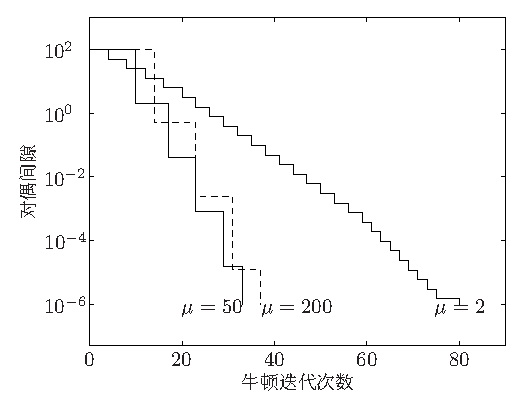
\includegraphics[width=.65\textwidth]{figures/ch11-15.pdf}
\caption*{图11.15 SOCP 的障碍法求解进展，展示对偶间隙与累计牛顿步数的关系。}
\end{figure}
用障碍法求解该问题，障碍函数为
\[
\phi(x)=-\sum_{i=1}^m\log\bigl((c_i^\T x+d_i)^2-\norm{A_i x+b_i}_2^2\bigr).
\]
中心化问题用牛顿法求解，算法参数与第11.3.2节例子相同：回溯参数 $\alpha=0.01$、$\beta=0.5$，停止准则为 $\lambda(x)^2/2\le10^{-5}$。

图11.15给出对偶间隙随累计牛顿步数的变化。它与线性规划和几何规划的图11.4与图11.6非常相似：每次中心化所需牛顿步数近似不变，因此对偶间隙近似线性收敛。对这个例子，只要 $\mu$ 至少约为 $10$，其选择对总牛顿步数也影响很小。与线性规划、几何规划的例子一样，$\mu$ 取 $10$ 至 $100$ 较合理，此时总牛顿步数约为 $30$，见图11.16。

\subsubsection*{小型 SDP}
下一个例子是 SDP
\begin{equation}\begin{aligned}\text{最小化}\quad&c^\T x\\\text{约束为}\quad&\sum_{i=1}^n x_iF_i+G\preceq0,
\end{aligned}\tag{11.46}\end{equation}
% Source PDF page 617 (printed p. 603)
变量为 $x\in\R^{100}$，且 $F_i\in\mathbf S^{100}$、$G\in\mathbf S^{100}$。随机生成实例，使其严格原始可行、严格对偶可行，且 $p^\star=1$。初始点位于中心路径上，对偶间隙为 $100$。

\begin{figure}[htbp]\centering
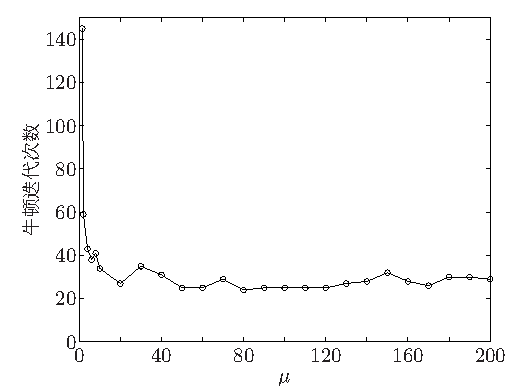
\includegraphics[width=.65\textwidth]{figures/ch11-16.pdf}
\caption*{图11.16 小型 SOCP 中参数 $\mu$ 的选择权衡。纵轴为将对偶间隙从 $100$ 降低到 $10^{-3}$ 所需的总牛顿步数，横轴为 $\mu$。}
\end{figure}
应用障碍法，对数障碍函数为
\[
\phi(x)=-\log\det\left(-\sum_{i=1}^n x_iF_i-G\right).
\]
图11.17展示了三个 $\mu$ 值下的障碍法进展。注意它与线性规划、几何规划、二阶锥规划的图11.4、图11.6和图11.15相似。与其他例子一样，只要 $\mu$ 不太小，它对效率的影响就很小。图11.18给出将对偶间隙缩小 $10^5$ 倍所需牛顿步数与 $\mu$ 的关系。

\subsubsection*{一族 SDP}
本节考察障碍法性能随问题维数的变化。考虑如下形式的一族 SDP：
\begin{equation}\begin{aligned}
\text{最小化}\quad&\one^\T x\\\text{约束为}\quad&A+\diag(x)\succeq0,
\end{aligned}\tag{11.47}\end{equation}
变量为 $x\in\R^n$，参数为 $A\in\mathbf S^n$。矩阵 $A$ 按如下方式生成：$i\ge j$ 时，从相互独立的 $\mathcal N(0,1)$ 分布生成 $A_{ij}$；$i<j$ 时取 $A_{ij}=A_{ji}$，使 $A\in\mathbf S^n$。再缩放 $A$，使其谱范数为 $1$。

% Source PDF page 618 (printed p. 604)
\begin{figure}[htbp]\centering
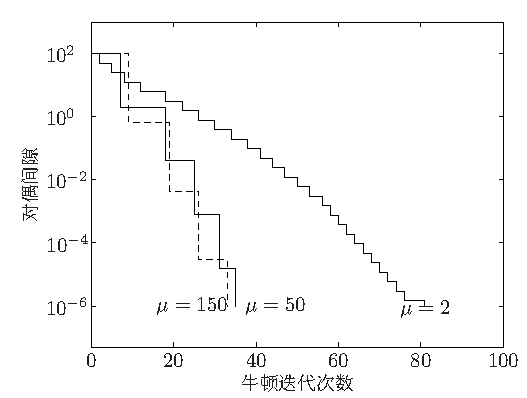
\includegraphics[width=.65\textwidth]{figures/ch11-17.pdf}
\caption*{图11.17 小型 SDP 的障碍法进展：对偶间隙与累计牛顿步数的关系。三条曲线分别对应 $\mu=2,50,150$。}
\end{figure}
\begin{figure}[htbp]\centering
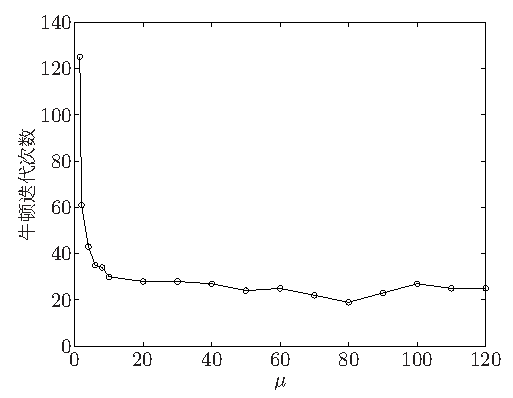
\includegraphics[width=.65\textwidth]{figures/ch11-18.pdf}
\caption*{图11.18 小型 SDP 中参数 $\mu$ 的选择权衡。纵轴为将对偶间隙从 $100$ 降低到 $10^{-3}$ 所需的总牛顿步数，横轴为 $\mu$。}
\end{figure}

% Source PDF page 619 (printed p. 605)
\begin{figure}[htbp]\centering
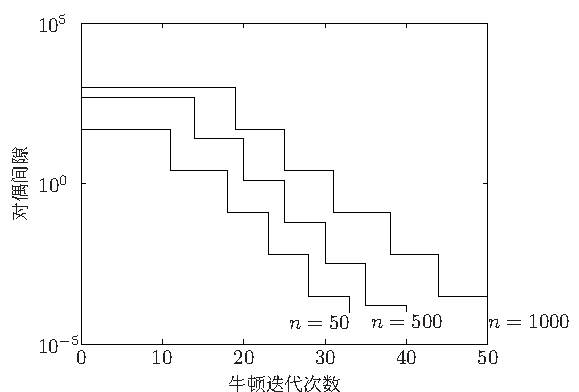
\includegraphics[width=.7\textwidth]{figures/ch11-19.pdf}
\caption*{图11.19 三个不同维数的随机 SDP (11.47) 的障碍法进展。图中展示对偶间隙与累计牛顿步数的关系，每个问题的变量数为 $n$。}
\end{figure}
算法参数取 $\mu=20$，中心化参数与上面各例相同：回溯参数 $\alpha=0.01$、$\beta=0.5$，停止准则 $\lambda(x)^2/2\le10^{-5}$。初始点位于中心路径上，$t^{(0)}=1$，即间隙为 $n$。当初始对偶间隙缩小 $8000$ 倍，即完成三次外迭代时，算法终止。

图11.19给出维数 $n=50$、$n=500$、$n=1000$ 的三个实例中，对偶间隙与迭代次数的关系。曲线与前面各图非常相似，也与 LP 的曲线非常相似。

为考察问题规模对所需牛顿步数的影响，对 $n=10$ 至 $n=1000$ 之间的 $20$ 个值，每个值生成 $100$ 个问题实例。用障碍法求解这 $2000$ 个问题，记录所需牛顿步数。图11.20汇总了每个 $n$ 下牛顿步数的均值与标准差。该图与 LP 的图11.8很相似。特别地，问题维数扩大 $100$ 倍时，所需牛顿步数增长很慢，仅从约 $20$ 次增加到 $26$ 次。

\subsection{基于自协调性的复杂度分析}
本节将第11.5节普通不等式问题的障碍法复杂度分析，推广到广义不等式问题。我们已经看到，外迭代次数为
\[
\left\lceil\frac{\log(\bar\theta/(t^{(0)}\epsilon))}{\log\mu}\right\rceil,
\]
% Source PDF page 620 (printed p. 606)
再加一次初始中心化。剩下需要界定每次中心化的牛顿步数，这将使用自协调函数的牛顿法复杂度理论。为简便起见，不计初始中心化的成本。

\begin{figure}[htbp]\centering
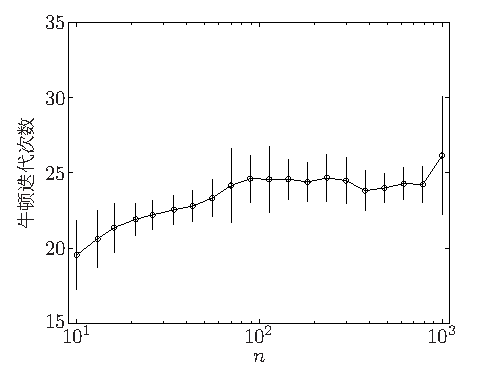
\includegraphics[width=.6\textwidth]{figures/ch11-20.pdf}
\caption*{图11.20 对问题规模 $n$ 的 $20$ 个值，每个值求解 $100$ 个随机 SDP (11.47) 所需的平均牛顿步数。误差棒给出每个 $n$ 下围绕均值的标准差。问题维数在 $100:1$ 的范围内变化时，平均牛顿步数的增长很小。}
\end{figure}
与第11.5节作相同假设：对所有 $t\ge t^{(0)}$，函数 $tf_0+\phi$ 为自协调闭函数，且 (11.38) 的下水平集有界。

\begin{origexample}{11.10}
\emph{二阶锥规划。} 函数
\[
-\psi(x)=-\log\left(x_{p+1}^2-\sum_{i=1}^p x_i^2\right)
\]
自协调（见例9.8），因此 SOCP (11.44) 的对数障碍函数 (11.45) 满足闭性和自协调性假设。
\end{origexample}

\begin{origexample}{11.11}
\emph{半定规划。} 以 $\log\det X$ 为半正定锥的广义对数时，一般半定规划满足自协调性假设。例如，标准形式 SDP
\[
\begin{aligned}\text{最小化}\quad&\tr(CX)\\\text{约束为}\quad&\tr(A_iX)=b_i,\quad i=1,\ldots,p,\\&X\succeq0,\end{aligned}
\]
变量为 $X\in\mathbf S^n$，对任意 $t^{(0)}\ge0$，函数 $t^{(0)}\tr(CX)-\log\det X$ 都是自协调闭函数。
\end{origexample}

% Source PDF page 621 (printed p. 607)
将看到，与标量情形完全一样，有
\begin{equation}\begin{aligned}
\mu t f_0(x^\star(t))+\phi(x^\star(t))-\mu t f_0(x^\star(\mu t))-\phi(x^\star(\mu t))
\le\bar\theta(\mu-1-\log\mu).
\end{aligned}\tag{11.48}\end{equation}
因此，自协调性与下水平集有界条件成立时，每次中心化所需的牛顿步数不超过
\[
\frac{\bar\theta(\mu-1-\log\mu)}\gamma+c,
\]
与普通不等式问题的障碍法完全相同。一旦建立基本界 (11.48)，广义不等式问题的复杂度分析就与普通不等式问题一致，唯一区别是以各锥次数之和 $\bar\theta$ 代替不等式数。

\subsubsection*{对偶锥的广义对数}
将用共轭函数证明界 (11.48)。设 $\psi$ 是正常锥 $K$ 的广义对数，次数为 $\theta$。凸函数 $-\psi$ 的共轭为
\[
(-\psi)^*(v)=\sup_u\bigl(v^\T u+\psi(u)\bigr).
\]
该函数为凸函数，定义域为 $-K^*=\{v\mid v\prec_{K^*}0\}$。定义 $\bar\psi$ 为
\begin{equation}
\bar\psi(v)=-(-\psi)^*(-v)=\inf_u\bigl(v^\T u-\psi(u)\bigr),\qquad
\dom\bar\psi=\operatorname{int}K^*.\tag{11.49}
\end{equation}
函数 $\bar\psi$ 为凹函数，实际上它也是对偶锥 $K^*$ 的广义对数，参数同样为 $\theta$，见习题11.17。称 $\bar\psi$ 为与广义对数 $\psi$ 对应的\emph{对偶对数}。

由 (11.49) 得到不等式
\begin{equation}
\bar\psi(v)+\psi(u)\le u^\T v,\tag{11.50}
\end{equation}
它对任意 $u\succ_K0$、$v\succ_{K^*}0$ 成立，等号成立当且仅当 $\nabla\psi(u)=v$，或等价地 $\nabla\bar\psi(v)=u$。（这只是凹函数版本 Young 不等式的一个变体。）

\begin{origexample}{11.12}
\emph{二阶锥。} 二阶锥的广义对数为
\[
\psi(x)=\log\left(x_{p+1}^2-\sum_{i=1}^p x_i^2\right),\qquad
\dom\psi=\left\{x\in\R^{p+1}\;\middle|\;x_{p+1}>\left(\sum_{i=1}^p x_i^2\right)^{1/2}\right\}.
\]
对应的对偶对数为
\[
\bar\psi(y)=\log\left(y_{p+1}^2-\sum_{i=1}^p y_i^2\right)+2-\log4,
\]
定义域为 $\dom\bar\psi=\{y\in\R^{p+1}\mid y_{p+1}>(\sum_{i=1}^p y_i^2)^{1/2}\}$，见习题3.36。除一个常数外，它与二阶锥原来的广义对数相同。
\end{origexample}

% Source PDF page 622 (printed p. 608)
\begin{origexample}{11.13}
\emph{半正定锥。} 与 $\psi(X)=\log\det X$、$\dom\psi=\mathbf S_{++}^p$ 对应的对偶对数为
\[
\bar\psi(Y)=\log\det Y+p,
\]
定义域为 $\dom\psi^*=\mathbf S_{++}^p$，见例3.23。同样，除一个常数外，它是同一个广义对数。
\end{origexample}

\subsubsection*{基本界的推导}
为简化记号，将 $x^\star(t)$ 记为 $x$，$x^\star(\mu t)$ 记为 $x^+$，$\lambda_i^\star(t)$ 记为 $\lambda_i$，$\nu^\star(t)$ 记为 $\nu$。由 (11.42) 中的 $t\lambda_i=\nabla\psi_i(-f_i(x))$ 以及性质 (11.43)，得到
\begin{equation}
\psi_i(-f_i(x))+\bar\psi_i(t\lambda_i)=-t\lambda_i^\T f_i(x)=\theta_i,\tag{11.51}
\end{equation}
即 (11.50) 对 $u=-f_i(x)$、$v=t\lambda_i$ 取等号。将同一不等式应用于 $u=-f_i(x^+)$、$v=\mu t\lambda_i$，得到
\[
\psi_i(-f_i(x^+))+\bar\psi_i(\mu t\lambda_i)\le-\mu t\lambda_i^\T f_i(x^+).
\]
利用 $\bar\psi_i$ 的对数齐次性，变为
\[
\psi_i(-f_i(x^+))+\bar\psi_i(t\lambda_i)+\theta_i\log\mu\le-\mu t\lambda_i^\T f_i(x^+).
\]
从这个不等式中减去等式 (11.51)，得到
\[
-\psi_i(-f_i(x))+\psi_i(-f_i(x^+))+\theta_i\log\mu
\le-\theta_i-\mu t\lambda_i^\T f_i(x^+).
\]
对 $i$ 求和，得到
\begin{equation}
\phi(x)-\phi(x^+)+\bar\theta\log\mu\le-\bar\theta-\mu t\sum_{i=1}^m\lambda_i^\T f_i(x^+).\tag{11.52}
\end{equation}
另由对偶函数的定义，
\begin{align*}
f_0(x)-\bar\theta/t&=g(\lambda,\nu)\\
&\le f_0(x^+)+\sum_{i=1}^m\lambda_i^\T f_i(x^+)+\nu^\T(Ax^+-b)\\
&=f_0(x^+)+\sum_{i=1}^m\lambda_i^\T f_i(x^+).
\end{align*}
将该不等式乘以 $\mu t$，再与 (11.52) 相加，得到
\[
\phi(x)-\phi(x^+)+\bar\theta\log\mu+\mu t f_0(x)-\mu\bar\theta
\le\mu t f_0(x^+)-\bar\theta.
\]
整理后为
\[
\mu t f_0(x)+\phi(x)-\mu t f_0(x^+)-\phi(x^+)\le\bar\theta(\mu-1-\log\mu),
\]
这就是所需不等式 (11.48)。

% Source PDF page 623 (printed p. 609)
\section{原始—对偶内点法}
本节介绍一种基本的原始—对偶内点法。原始—对偶内点法与障碍法很相似，但有如下区别。
\begin{itemize}
\item 只有一层循环或迭代，不像障碍法那样区分内迭代和外迭代。每次迭代同时更新原始变量与对偶变量。
\item 原始—对偶内点法对修改后的 KKT 方程，即对数障碍中心化问题的最优性条件，应用牛顿法得到搜索方向。原始—对偶搜索方向与障碍法产生的搜索方向相似，但并不完全相同。
\item 原始—对偶内点法的原始迭代点和对偶迭代点不一定可行。
\end{itemize}
原始—对偶内点法通常比障碍法更有效，特别是在要求高精度时，因为它们可以表现出快于线性的收敛速度。对线性规划、二次规划、二阶锥规划、几何规划和半定规划等几类基本问题，专门设计的原始—对偶方法优于障碍法。对一般非线性凸优化问题，原始—对偶内点法仍是活跃的研究课题，但前景很好。它相对障碍法的另一个优点，是在问题可行但不严格可行时也能工作，不过这里不再深入讨论。

本节给出求解 (11.1) 的一种基本原始—对偶方法，不作收敛性分析。关于原始—对偶方法及其收敛性分析的更全面论述，请参阅参考文献。

\subsection{原始—对偶搜索方向}
与障碍法一样，从修改后的 KKT 条件 (11.15) 出发，将其写为 $r_t(x,\lambda,\nu)=0$，其中定义
\begin{equation}
r_t(x,\lambda,\nu)=\begin{bmatrix}
\nabla f_0(x)+Df(x)^\T\lambda+A^\T\nu\\
-\diag(\lambda)f(x)-(1/t)\one\\
Ax-b
\end{bmatrix},\tag{11.53}
\end{equation}
且 $t>0$。这里 $f:\R^n\to\R^m$ 及其导数矩阵 $Df$ 为
\[
f(x)=\begin{bmatrix}f_1(x)\\\vdots\\f_m(x)\end{bmatrix},\qquad
Df(x)=\begin{bmatrix}\nabla f_1(x)^\T\\\vdots\\\nabla f_m(x)^\T\end{bmatrix}.
\]
若 $x,\lambda,\nu$ 满足 $r_t(x,\lambda,\nu)=0$，且 $f_i(x)<0$，则 $x=x^\star(t)$、$\lambda=\lambda^\star(t)$、$\nu=\nu^\star(t)$。特别地，$x$ 原始可行，$\lambda,\nu$ 对偶可行，
% Source PDF page 624 (printed p. 610)
对偶间隙为 $m/t$。$r_t$ 的第一个分块
\[
r_{\mathrm{dual}}=\nabla f_0(x)+Df(x)^\T\lambda+A^\T\nu
\]
称为\emph{对偶残差}，最后一个分块 $r_{\mathrm{pri}}=Ax-b$ 称为\emph{原始残差}。中间分块
\[
r_{\mathrm{cent}}=-\diag(\lambda)f(x)-(1/t)\one
\]
是\emph{中心性残差}，即修改后互补条件的残差。

现在固定 $t$，在满足 $f(x)\prec0$、$\lambda\succ0$ 的点 $(x,\lambda,\nu)$ 处，考虑求解非线性方程 $r_t(x,\lambda,\nu)=0$ 的牛顿步，不像第11.3.4节那样预先消去 $\lambda$。分别将当前点和牛顿步记为
\[
y=(x,\lambda,\nu),\qquad\Delta y=(\Delta x,\Delta\lambda,\Delta\nu).
\]
牛顿步由线性方程
\[
r_t(y+\Delta y)\approx r_t(y)+Dr_t(y)\Delta y=0
\]
刻画，即 $\Delta y=-Dr_t(y)^{-1}r_t(y)$。用 $x,\lambda,\nu$ 表示，得到
\begin{equation}
\begin{bmatrix}
\nabla^2 f_0(x)+\sum_{i=1}^m\lambda_i\nabla^2 f_i(x)&Df(x)^\T&A^\T\\
-\diag(\lambda)Df(x)&-\diag(f(x))&0\\
A&0&0
\end{bmatrix}
\begin{bmatrix}\Delta x\\\Delta\lambda\\\Delta\nu\end{bmatrix}
=-\begin{bmatrix}r_{\mathrm{dual}}\\r_{\mathrm{cent}}\\r_{\mathrm{pri}}\end{bmatrix}.
\tag{11.54}
\end{equation}
\emph{原始—对偶搜索方向} $\Delta y_{\mathrm{pd}}=(\Delta x_{\mathrm{pd}},\Delta\lambda_{\mathrm{pd}},\Delta\nu_{\mathrm{pd}})$ 定义为 (11.54) 的解。

原始搜索方向和对偶搜索方向通过系数矩阵与残差相互耦合。例如，原始搜索方向 $\Delta x_{\mathrm{pd}}$ 既依赖 $x$，也依赖当前对偶变量 $\lambda,\nu$。还应注意，若 $x$ 满足 $Ax=b$，即原始可行性残差 $r_{\mathrm{pri}}$ 为零，则 $A\Delta x_{\mathrm{pd}}=0$，所以 $\Delta x_{\mathrm{pd}}$ 是原始可行方向：对任意 $s$，$x+s\Delta x_{\mathrm{pd}}$ 都满足 $A(x+s\Delta x_{\mathrm{pd}})=b$。

\subsubsection*{与障碍法搜索方向的比较}
原始—对偶搜索方向与障碍法使用的搜索方向关系密切，但并不完全相同。从定义原始—对偶搜索方向的线性方程 (11.54) 出发，利用第二组分块方程给出的
\[
\Delta\lambda_{\mathrm{pd}}=-\diag(f(x))^{-1}\diag(\lambda)Df(x)\Delta x_{\mathrm{pd}}
+\diag(f(x))^{-1}r_{\mathrm{cent}},
\]
消去变量 $\Delta\lambda_{\mathrm{pd}}$。将它代入第一组分块方程，得到
\begin{equation}\begin{aligned}
\begin{bmatrix}H_{\mathrm{pd}}&A^\T\\A&0\end{bmatrix}
\begin{bmatrix}\Delta x_{\mathrm{pd}}\\\Delta\nu_{\mathrm{pd}}\end{bmatrix}
&=-\begin{bmatrix}r_{\mathrm{dual}}+Df(x)^\T\diag(f(x))^{-1}r_{\mathrm{cent}}\\r_{\mathrm{pri}}\end{bmatrix}\\
&=-\begin{bmatrix}\nabla f_0(x)+(1/t)\sum_{i=1}^m\frac1{-f_i(x)}\nabla f_i(x)+A^\T\nu\\r_{\mathrm{pri}}\end{bmatrix},
\end{aligned}\tag{11.55}\end{equation}
% Source PDF page 625 (printed p. 611)
其中
\begin{equation}
H_{\mathrm{pd}}=\nabla^2 f_0(x)+\sum_{i=1}^m\lambda_i\nabla^2 f_i(x)
+\sum_{i=1}^m\frac{\lambda_i}{-f_i(x)}\nabla f_i(x)\nabla f_i(x)^\T.\tag{11.56}
\end{equation}
将 (11.55) 与方程 (11.14) 比较，后者定义了障碍法参数为 $t$ 时中心化问题的牛顿步。它可以写为
\begin{equation}\begin{aligned}
\begin{bmatrix}H_{\mathrm{bar}}&A^\T\\A&0\end{bmatrix}
\begin{bmatrix}\Delta x_{\mathrm{bar}}\\\nu_{\mathrm{bar}}\end{bmatrix}
&=-\begin{bmatrix}t\nabla f_0(x)+\nabla\phi(x)\\r_{\mathrm{pri}}\end{bmatrix}\\
&=-\begin{bmatrix}t\nabla f_0(x)+\sum_{i=1}^m\frac1{-f_i(x)}\nabla f_i(x)\\r_{\mathrm{pri}}\end{bmatrix},
\end{aligned}\tag{11.57}\end{equation}
其中
\begin{equation}
H_{\mathrm{bar}}=t\nabla^2 f_0(x)+\sum_{i=1}^m\frac1{-f_i(x)}\nabla^2 f_i(x)
+\sum_{i=1}^m\frac1{f_i(x)^2}\nabla f_i(x)\nabla f_i(x)^\T.\tag{11.58}
\end{equation}
这里给出了不可行牛顿步的一般表达式。若当前 $x$ 可行，即 $r_{\mathrm{pri}}=0$，则 $\Delta x_{\mathrm{bar}}$ 与 (11.14) 定义的可行牛顿步 $\Delta x_{\mathrm{nt}}$ 一致。

首先，两个方程组 (11.55) 和 (11.57) 非常相似。它们的系数矩阵具有相同结构：$H_{\mathrm{pd}}$ 与 $H_{\mathrm{bar}}$ 都是矩阵
\[
\nabla^2 f_0(x),\quad\nabla^2 f_1(x),\ldots,\nabla^2 f_m(x),\quad
\nabla f_1(x)\nabla f_1(x)^\T,\ldots,\nabla f_m(x)\nabla f_m(x)^\T
\]
的正线性组合。这意味着可以用同一种方法计算原始—对偶搜索方向和障碍法牛顿步。

关于原始—对偶方程 (11.55) 与障碍法方程 (11.57) 的关系，还可以进一步说明。将 (11.57) 第一组分块方程除以 $t$，并定义变量 $\Delta\nu_{\mathrm{bar}}=(1/t)\nu_{\mathrm{bar}}-\nu$，其中 $\nu$ 任意，得到
\[
\begin{bmatrix}(1/t)H_{\mathrm{bar}}&A^\T\\A&0\end{bmatrix}
\begin{bmatrix}\Delta x_{\mathrm{bar}}\\\Delta\nu_{\mathrm{bar}}\end{bmatrix}
=-\begin{bmatrix}\nabla f_0(x)+(1/t)\sum_{i=1}^m\frac1{-f_i(x)}\nabla f_i(x)+A^\T\nu\\r_{\mathrm{pri}}\end{bmatrix}.
\]
这个形式的右端与在相同 $x,\lambda,\nu$ 处计算的原始—对偶方程右端一致。系数矩阵仅在 $(1,1)$ 分块有所不同：
\begin{align*}
H_{\mathrm{pd}}&=\nabla^2 f_0(x)+\sum_{i=1}^m\lambda_i\nabla^2 f_i(x)
+\sum_{i=1}^m\frac{\lambda_i}{-f_i(x)}\nabla f_i(x)\nabla f_i(x)^\T,\\
(1/t)H_{\mathrm{bar}}&=\nabla^2 f_0(x)+\sum_{i=1}^m\frac1{-tf_i(x)}\nabla^2 f_i(x)
+\sum_{i=1}^m\frac1{tf_i(x)^2}\nabla f_i(x)\nabla f_i(x)^\T.
\end{align*}
当 $x$ 与 $\lambda$ 满足 $-f_i(x)\lambda_i=1/t$ 时，系数矩阵相同，搜索方向因而也相同。

% Source PDF page 626 (printed p. 612)
\subsection{代理对偶间隙}
原始—对偶内点法中的迭代点 $x^{(k)},\lambda^{(k)},\nu^{(k)}$ 不一定可行，只有算法收敛的极限点才可行。这意味着，无法像障碍法的外迭代那样，容易地计算算法第 $k$ 步对应的对偶间隙 $\eta^{(k)}$。取而代之，对于任意满足 $f(x)\prec0$、$\lambda\succeq0$ 的 $x,\lambda$，定义\emph{代理对偶间隙}
\begin{equation}
\widehat\eta(x,\lambda)=-f(x)^\T\lambda.\tag{11.59}
\end{equation}
如果 $x$ 原始可行、$\lambda,\nu$ 对偶可行，即 $r_{\mathrm{pri}}=0$、$r_{\mathrm{dual}}=0$，则代理间隙 $\widehat\eta$ 就是对偶间隙。注意，与代理对偶间隙 $\widehat\eta$ 对应的参数 $t$ 为 $m/\widehat\eta$。

\subsection{原始—对偶内点法}
现在可以给出基本原始—对偶内点算法。

\begin{origalgorithm}{11.2}
\textbf{原始—对偶内点法。}

给定满足 $f_1(x)<0,\ldots,f_m(x)<0$ 的 $x$，以及 $\lambda\succ0$、$\mu>1$、$\epsilon_{\mathrm{feas}}>0$、$\epsilon>0$。

重复：
\begin{enumerate}
\item \textbf{确定 $t$。} 取 $t:=\mu m/\widehat\eta$。
\item \textbf{计算原始—对偶搜索方向} $\Delta y_{\mathrm{pd}}$。
\item \textbf{线搜索与更新。} 确定步长 $s>0$，取 $y:=y+s\Delta y_{\mathrm{pd}}$。
\end{enumerate}
直至 $\norm{r_{\mathrm{pri}}}_2\le\epsilon_{\mathrm{feas}}$、$\norm{r_{\mathrm{dual}}}_2\le\epsilon_{\mathrm{feas}}$，并且 $\widehat\eta\le\epsilon$。
\end{origalgorithm}
第1步把参数 $t$ 设为 $m/\widehat\eta$ 的 $\mu$ 倍，其中 $m/\widehat\eta$ 是与当前代理对偶间隙对应的 $t$ 值。若 $x,\lambda,\nu$ 是参数 $t$ 对应的中心点，因而对偶间隙为 $m/t$，则第1步将 $t$ 增大 $\mu$ 倍，这与障碍法的更新完全相同。参数 $\mu$ 取约为 $10$ 的值似乎效果很好。

当 $x$ 原始可行、$\lambda,\nu$ 对偶可行（容差内，容差为 $\epsilon_{\mathrm{feas}}$），并且代理间隙小于容差 $\epsilon$ 时，原始—对偶内点算法终止。由于原始—对偶内点法经常快于线性收敛，通常会取较小的 $\epsilon_{\mathrm{feas}}$ 与 $\epsilon$。

\subsubsection*{线搜索}
原始—对偶内点法采用基于残差范数的标准回溯线搜索，并作修改以保证 $\lambda\succ0$、$f(x)\prec0$。当前迭代点记为 $x,\lambda,\nu$，下一迭代点记为 $x^+,\lambda^+,\nu^+$，即
\[
x^+=x+s\Delta x_{\mathrm{pd}},\qquad
\lambda^+=\lambda+s\Delta\lambda_{\mathrm{pd}},\qquad
\nu^+=\nu+s\Delta\nu_{\mathrm{pd}}.
\]
% Source PDF page 627 (printed p. 613)
在 $y^+$ 处计算的残差记为 $r^+$。

首先计算不超过 $1$ 且使 $\lambda^+\succeq0$ 的最大正步长，即
\begin{align*}
s_{\mathrm{max}}&=\sup\{s\in[0,1]\mid\lambda+s\Delta\lambda\succeq0\}\\
&=\min\bigl\{1,\min\{-\lambda_i/\Delta\lambda_i\mid\Delta\lambda_i<0\}\bigr\}.
\end{align*}
回溯从 $s=0.99s_{\mathrm{max}}$ 开始，反复将 $s$ 乘以 $\beta\in(0,1)$，直至 $f(x^+)\prec0$。继续将 $s$ 乘以 $\beta$，直至
\[
\norm{r_t(x^+,\lambda^+,\nu^+)}_2\le(1-\alpha s)\norm{r_t(x,\lambda,\nu)}_2.
\]
回溯参数 $\alpha,\beta$ 的常见取法与牛顿法相同：$\alpha$ 通常在 $0.01$ 至 $0.1$ 之间，$\beta$ 通常在 $0.3$ 至 $0.8$ 之间。

原始—对偶内点算法的一次迭代，相当于不可行牛顿法为求解 $r_t(x,\lambda,\nu)=0$ 而执行的一步，只是修改为保证 $\lambda\succ0$、$f(x)\prec0$；等价地，将 $r_t$ 的定义域限制为 $\lambda\succ0$、$f(x)\prec0$。用不可行初始点牛顿法收敛性证明中的相同论证，可以说明原始—对偶方法的线搜索总在有限步内终止。

\subsection{例子}
用第11.3.2节的相同问题展示原始—对偶内点法的性能。唯一区别是，这里不像第11.3.2节那样从中心路径上的点出发，而是随机生成满足 $f(x)\prec0$ 的 $x^{(0)}$，并取 $\lambda_i^{(0)}=-1/f_i(x^{(0)})$，因此初始代理间隙为 $\widehat\eta=100$。使用的原始—对偶内点法参数为
\[
\mu=10,\qquad\beta=0.5,\qquad\epsilon=10^{-8},\qquad\alpha=0.01.
\]

\subsubsection*{小型 LP 与 GP}
首先考虑第11.3.2节的小型 LP，包含 $m=100$ 个不等式和 $n=50$ 个变量。图11.21展示原始—对偶内点法的进展，给出了代理间隙 $\widehat\eta$ 和原始、对偶残差范数
\[
r_{\mathrm{feas}}=\left(\norm{r_{\mathrm{pri}}}_2^2+\norm{r_{\mathrm{dual}}}_2^2\right)^{1/2}
\]
随迭代次数变化的两条曲线。初始点原始可行，所以图中反映的是对偶可行性残差的范数。曲线表明，残差迅速趋于零，$24$ 次迭代后在数值精度范围内为零。代理间隙也迅速收敛。与障碍法相比，原始—对偶内点法更快，特别是在要求高精度时。

图11.22给出了原始—对偶内点法求解第11.3.2节 GP 的进展，收敛情况与 LP 相似。

% Source PDF page 628 (printed p. 614)
\begin{figure}[htbp]\centering
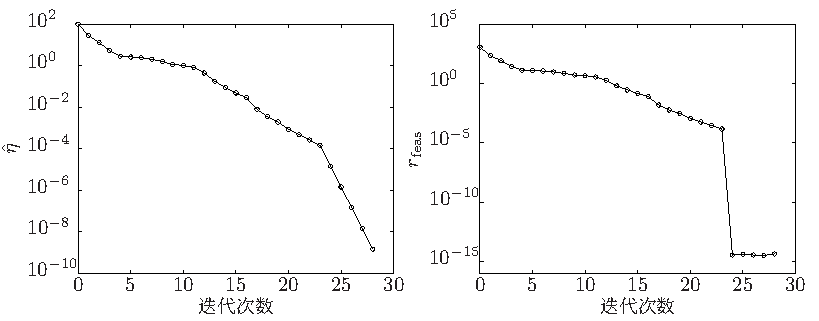
\includegraphics[width=.95\textwidth]{figures/ch11-21.pdf}
\caption*{图11.21 原始—对偶内点法求解 LP 的进展：代理对偶间隙 $\widehat\eta$ 以及原始、对偶残差范数与迭代次数的关系。残差在 $24$ 次迭代内迅速收敛到零；代理间隙也在约 $28$ 次迭代后收敛到很小的值。原始—对偶内点法比障碍法收敛更快，特别是在要求高精度时。}
\end{figure}
\begin{figure}[htbp]\centering
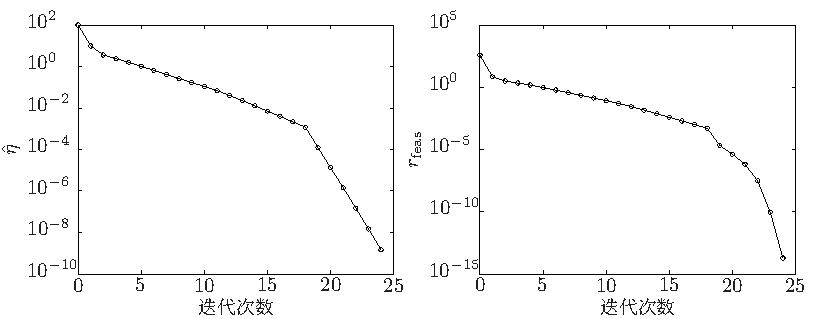
\includegraphics[width=.95\textwidth]{figures/ch11-22.pdf}
\caption*{图11.22 原始—对偶内点法求解 GP 的进展：代理对偶间隙 $\widehat\eta$ 以及原始、对偶残差范数与迭代次数的关系。}
\end{figure}

% Source PDF page 629 (printed p. 615)
\begin{figure}[htbp]\centering
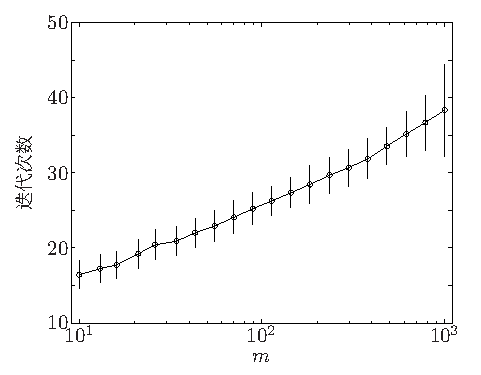
\includegraphics[width=.6\textwidth]{figures/ch11-23.pdf}
\caption*{图11.23 求解不同维数随机标准 LP 所需的迭代次数，$n=2m$。误差棒给出每个维数的 $100$ 个实例中围绕均值的标准差。问题维数变化 $100$ 倍时，所需迭代次数近似按对数增长。}
\end{figure}

\subsubsection*{一族 LP}
这里使用第11.3.2节相同的一族标准形式 LP，考察原始—对偶方法的性能与问题维数的关系。用原始—对偶内点法求解同样的 $2000$ 个实例，每个 $m$ 值对应 $100$ 个实例。算法从 $x^{(0)}=\one$、$\lambda^{(0)}=\one$、$\nu^{(0)}=0$ 出发，终止容差为 $\epsilon=10^{-8}$。图11.23给出所需迭代次数的均值与标准差随 $m$ 的变化。迭代次数从 $15$ 到 $35$，近似随 $m$ 的对数增长。与图11.8的障碍法结果比较可见，尽管我们从不可行初始点出发，并将问题求到高得多的精度，原始—对偶方法的迭代次数也只略多一些。

% Source PDF page 629 (printed p. 615), section 11.8 begins here.
\section{实现}
障碍法的主要计算工作，是计算中心化问题的牛顿步，即求解如下形式的线性方程组：
\begin{equation}
\begin{bmatrix}H&A^\T\\A&0\end{bmatrix}
\begin{bmatrix}\Delta x_{\mathrm{nt}}\\\nu_{\mathrm{nt}}\end{bmatrix}
=-\begin{bmatrix}g\\0\end{bmatrix},\tag{11.60}
\end{equation}
其中
\[
H=t\nabla^2 f_0(x)+\sum_{i=1}^m\frac1{f_i(x)^2}\nabla f_i(x)\nabla f_i(x)^\T
+\sum_{i=1}^m\frac1{-f_i(x)}\nabla^2 f_i(x),
\]
% Source PDF page 630 (printed p. 616)
\[
g=t\nabla f_0(x)+\sum_{i=1}^m\frac1{-f_i(x)}\nabla f_i(x).
\]
原始—对偶方法的牛顿方程具有完全相同的结构，所以本节的讨论也适用于原始—对偶方法。

(11.60) 的系数矩阵具有 KKT 结构，因此第9.7节和第10.4节的全部讨论都适用。特别地，可以用消元求解，并利用稀疏性、对角加低秩等结构。下面给出几个常见例子，利用 KKT 方程的特殊结构更有效地计算牛顿步。

\subsubsection*{稀疏问题}
如果原问题稀疏，即目标函数与每个约束函数各自只依赖少量变量，则目标函数和约束函数的梯度、Hessian 矩阵都稀疏，系数矩阵 $A$ 也稀疏。只要 $m$ 不太大，矩阵 $H$ 很可能也稀疏，因此可以用稀疏矩阵方法计算牛顿步。即便 KKT 矩阵中有少数较稠密的行和列，这种方法也很可能效果不错；例如，少数等式约束涉及大量变量时，就会出现这种情况。

\subsubsection*{可分目标与少量线性不等式约束}
假设目标函数可分，而且线性等式与不等式约束相对较少。此时 $\nabla^2 f_0(x)$ 为对角矩阵，$\nabla^2 f_i(x)$ 各项为零，因此 $H$ 是对角加低秩矩阵。由于 $H$ 容易求逆，可以高效求解 KKT 方程。只要 $\nabla^2 f_0(x)$ 容易求逆，例如它是带状、稀疏或分块对角矩阵，就可以使用同样的方法。

\subsection{标准形式线性规划}
首先讨论标准形式 LP 的障碍法实现：
\[
\begin{aligned}\text{最小化}\quad&c^\T x\\\text{约束为}\quad&Ax=b,\qquad x\succeq0,\end{aligned}
\]
其中 $A\in\R^{m\times n}$。中心化问题
\[
\begin{aligned}\text{最小化}\quad&tc^\T x-\sum_{i=1}^n\log x_i\\\text{约束为}\quad&Ax=b\end{aligned}
\]
的牛顿方程为
\[
\begin{bmatrix}\diag(x)^{-2}&A^\T\\A&0\end{bmatrix}
\begin{bmatrix}\Delta x_{\mathrm{nt}}\\\nu_{\mathrm{nt}}\end{bmatrix}
=\begin{bmatrix}-tc+\diag(x)^{-1}\one\\0\end{bmatrix}.
\]

% Source PDF page 631 (printed p. 617)
通常通过分块消去 $\Delta x_{\mathrm{nt}}$ 来求解。由第一个方程，
\begin{align*}
\Delta x_{\mathrm{nt}}&=\diag(x)^2(-tc+\diag(x)^{-1}\one-A^\T\nu_{\mathrm{nt}})\\
&=-t\diag(x)^2c+x-\diag(x)^2A^\T\nu_{\mathrm{nt}}.
\end{align*}
代入第二个方程，得到
\[
A\diag(x)^2A^\T\nu_{\mathrm{nt}}=-tA\diag(x)^2c+b.
\]
由于假设 $\rank A=m$，系数矩阵为正定矩阵。此外，若 $A$ 稀疏，则 $A\diag(x)^2A^\T$ 通常也稀疏，可以使用稀疏 Cholesky 分解。

\subsection{\texorpdfstring{$\ell_1$}{ℓ₁} 范数逼近}
考虑 $\ell_1$ 范数逼近问题
\[
\text{最小化}\quad\norm{Ax-b}_1,
\]
其中 $A\in\R^{m\times n}$。假设 $m,n$ 很大，$A$ 具有稀疏性等结构，讨论其实现，并与相应最小二乘问题
\[
\text{最小化}\quad\norm{Ax-b}_2^2
\]
的成本比较。

首先引入辅助变量 $y\in\R^m$，将 $\ell_1$ 范数逼近问题写成 LP：
\[
\begin{aligned}
\text{最小化}\quad&\one^\T y\\
\text{约束为}\quad&\begin{bmatrix}A&-\I\\-A&-\I\end{bmatrix}\begin{bmatrix}x\\y\end{bmatrix}
\preceq\begin{bmatrix}b\\-b\end{bmatrix}.
\end{aligned}
\]
中心化问题的牛顿方程为
\[
\begin{bmatrix}A^\T&-A^\T\\-\I&-\I\end{bmatrix}
\begin{bmatrix}D_1&0\\0&D_2\end{bmatrix}
\begin{bmatrix}A&-\I\\-A&-\I\end{bmatrix}
\begin{bmatrix}\Delta x_{\mathrm{nt}}\\\Delta y_{\mathrm{nt}}\end{bmatrix}
=-\begin{bmatrix}A^\T g_1\\g_2\end{bmatrix},
\]
其中
\[
D_1=\diag(b-Ax+y)^{-2},\qquad D_2=\diag(-b+Ax+y)^{-2},
\]
而
\begin{align*}
g_1&=\diag(b-Ax+y)^{-1}\one-\diag(-b+Ax+y)^{-1}\one,\\
g_2&=t\one-\diag(b-Ax+y)^{-1}\one-\diag(-b+Ax+y)^{-1}\one.
\end{align*}
将左端乘开，可以化简为
\[
\begin{bmatrix}A^\T(D_1+D_2)A&-A^\T(D_1-D_2)\\-(D_1-D_2)A&D_1+D_2\end{bmatrix}
\begin{bmatrix}\Delta x_{\mathrm{nt}}\\\Delta y_{\mathrm{nt}}\end{bmatrix}
=-\begin{bmatrix}A^\T g_1\\g_2\end{bmatrix}.
\]

% Source PDF page 632 (printed p. 618)
分块消去 $\Delta y_{\mathrm{nt}}$，约化为
\begin{equation}
A^\T DA\Delta x_{\mathrm{nt}}=-A^\T g,\tag{11.61}
\end{equation}
其中
\[
D=4D_1D_2(D_1+D_2)^{-1}=2\bigl(\diag(y)^2+\diag(b-Ax)^2\bigr)^{-1},
\]
且
\[
g=g_1+(D_1-D_2)(D_1+D_2)^{-1}g_2.
\]
求出 $\Delta x_{\mathrm{nt}}$ 后，由
\[
\Delta y_{\mathrm{nt}}=(D_1+D_2)^{-1}\bigl(-g_2+(D_1-D_2)A\Delta x_{\mathrm{nt}}\bigr)
\]
得到 $\Delta y_{\mathrm{nt}}$。

有意思的是，(11.61) 正是加权最小二乘问题
\[
\text{最小化}\quad\norm{D^{1/2}(A\Delta x+D^{-1}g)}_2
\]
的正规方程。换言之，求解 $\ell_1$ 范数逼近问题的成本，就是求解少量加权最小二乘问题的成本，矩阵 $A$ 相同，但权重逐次迭代变化。若 $A$ 的结构允许快速求解最小二乘问题，例如可利用稀疏性，那么也能快速求解 (11.61)。

\subsection{不等式形式的半定规划}
考虑 SDP
\[
\begin{aligned}\text{最小化}\quad&c^\T x\\\text{约束为}\quad&\sum_{i=1}^n x_iF_i+G\preceq0,\end{aligned}
\]
变量为 $x\in\R^n$，参数为 $F_1,\ldots,F_n,G\in\mathbf S^p$。采用对数行列式障碍函数，相应中心化问题为
\[
\text{最小化}\quad tc^\T x-\log\det\left(-\sum_{i=1}^n x_iF_i-G\right).
\]
牛顿步 $\Delta x_{\mathrm{nt}}$ 由 $H\Delta x_{\mathrm{nt}}=-g$ 求得，其中 Hessian 矩阵与梯度为
\begin{align*}
H_{ij}&=\tr(S^{-1}F_iS^{-1}F_j),\quad i,j=1,\ldots,n,\\
g_i&=tc_i+\tr(S^{-1}F_i),\quad i=1,\ldots,n,
\end{align*}
这里 $S=-\sum_{i=1}^n x_iF_i-G$。一种标准做法是先形成 $H$ 与 $g$，再用 Cholesky 分解求解牛顿方程。

先考察无结构情形，即假设所有矩阵都稠密，并且只记录浮点运算次数关于维数 $n,p$ 的阶数。首先形成 $S$，成本为 $np^2$ 阶。然后对 $S$ 作 Cholesky 分解，再对 $F_i$ 各列回代，计算每个 $S^{-1}F_i$；也可以先形成 $S^{-1}$ 再乘 $F_i$。每个 $i$ 的成本为 $p^3$ 阶，因此总成本为 $np^3$ 阶。最后，
% Source PDF page 633 (printed p. 619)
将 $H_{ij}$ 作为矩阵 $S^{-1}F_i$ 与 $S^{-1}F_j$ 的内积计算，成本为 $p^2$ 阶。共有 $n(n+1)/2$ 对，总成本为 $n^2p^2$ 阶。求出牛顿方向的成本为 $n^3$ 阶。因此，主导阶数为 $\max\{np^3,n^2p^2,n^3\}$。

一般不能利用矩阵 $F_i,G$ 的稀疏性，因为即使 $F_i,G$ 稀疏，$H$ 也通常稠密。一个例外是 $F_i,G$ 具有相同的分块对角结构，此时上述全部运算都可以逐块完成。

不过，通常可以利用 $F_i,G$ 共有的稀疏性，更高效地形成稠密 Hessian 矩阵 $H$。若能找到一种排列，使 $S$ 的 Cholesky 因子相当稀疏，就能高效计算 $S^{-1}F_i$，从而以高得多的效率形成 $H_{ij}$。

一个经常出现的有意思例子，是带矩阵不等式
\[
\diag(x)\preceq B
\]
的 SDP。此时 $F_i=E_{ii}$，其中 $E_{ii}$ 是 $(i,i)$ 元为 $1$、其余元素均为零的矩阵。$H$ 可以非常高效地求出：
\[
H_{ij}=(S^{-1})_{ij}^2,
\]
其中 $S=B-\diag(x)$。因此形成 $H$ 的成本就是形成 $S^{-1}$ 的成本，至多为 $n^3$ 阶，即不利用任何其他结构时的成本。

\subsection{网络速率优化}
考虑第10.4.3节（第550页）最优网络流问题的一个变体，有时称为\emph{网络速率优化问题}。网络表示为有向图，有 $L$ 条弧或链路。货物或信息分组在网络中沿链路传输。网络支持 $n$ 条流，其非负速率 $x_1,\ldots,x_n$ 是优化变量。每条流从源节点沿固定或预先指定的路径，即路由，到达目的节点。一条链路可以同时承载多条流，其总流量是经过它的各流速率之和。每条链路具有正容量，表示它能处理的最大总流量。

用流—链路关联矩阵 $A\in\R^{L\times n}$ 表示这些容量限制，定义
\[
A_{ij}=\begin{cases}1,&\text{流 $j$ 经过链路 $i$},\\0,&\text{否则}.\end{cases}
\]
链路 $i$ 的总流量为 $(Ax)_i$，因此链路容量约束可写为 $Ax\preceq c$，其中 $c_i$ 是链路 $i$ 的容量。通常每条路径只经过全部链路中的很少一部分，因此 $A$ 稀疏。

在网络速率问题中，路径固定，并编码在作为参数的矩阵 $A$ 中；变量为流速率 $x_i$。目标
% Source PDF page 634 (printed p. 620)
是选择流速率，使可分效用函数
\[
U(x)=U_1(x_1)+\cdots+U_n(x_n)
\]
最大。假设每个 $U_i$，因而 $U$，都为凹且非减函数。可以将 $U_i(x_i)$ 看作以速率 $x_i$ 支持第 $i$ 条流获得的收入，$U(x)$ 则是全部流带来的总收入。网络速率优化问题为
\begin{equation}\begin{aligned}
\text{最大化}\quad&U(x)\\\text{约束为}\quad&Ax\preceq c,\qquad x\succeq0,
\end{aligned}\tag{11.62}\end{equation}
它是凸优化问题。

用障碍法求解。每步都必须用牛顿法最小化如下形式的函数：
\[
-tU(x)-\sum_{i=1}^L\log(c-Ax)_i-\sum_{j=1}^n\log x_j.
\]
牛顿步 $\Delta x_{\mathrm{nt}}$ 由线性方程
\[
(D_0+A^\T D_1A+D_2)\Delta x_{\mathrm{nt}}=-g
\]
求得，其中
\begin{align*}
D_0&=-t\diag(U_1''(x),\ldots,U_n''(x)),\\
D_1&=\diag(1/(c-Ax)_1^2,\ldots,1/(c-Ax)_L^2),\\
D_2&=\diag(1/x_1^2,\ldots,1/x_n^2)
\end{align*}
为对角矩阵，且 $g\in\R^n$。这个 $n\times n$ 系数矩阵的稀疏结构可以精确刻画：
\[
(D_0+A^\T D_1A+D_2)_{ij}\ne0
\]
当且仅当流 $i$ 与流 $j$ 共用一条链路。如果路径较短，而且每条链路只经过较少路径，则该矩阵稀疏，可以使用稀疏 Cholesky 分解。如果有少数较稠密的行列，仍可以高效求解牛顿系统。少数流与许多其他流相交时会出现这种情况，例如少数流路径较长时。

也可以利用矩阵求逆引理，通过求解系数矩阵为 $L\times L$ 的方程组计算牛顿步，其形式为
\[
\bigl(D_1^{-1}+A(D_0+D_2)^{-1}A^\T\bigr)y=-A(D_0+D_2)^{-1}g,
\]
然后计算
\[
\Delta x_{\mathrm{nt}}=-(D_0+D_2)^{-1}(g+A^\T y).
\]
这里也可精确描述稀疏模式：
\[
\bigl(D_1^{-1}+A(D_0+D_2)^{-1}A^\T\bigr)_{ij}\ne0
\]
当且仅当存在一条路径同时经过链路 $i$ 和链路 $j$。若大多数路径较短，该矩阵稀疏。若存在少数瓶颈，即少数链路承载了许多流，则该矩阵稀疏，但有少数稠密行列。

% Source PDF page 635 (printed p. 621)
\section*{文献说明}
\addcontentsline{toc}{section}{文献说明}
Fiacco 和 McCormick [FM90, 第1.2节] 详细介绍了障碍法的早期历史。20世纪60年代，它与一些密切相关的技术一起成为流行的凸优化算法，包括中心法（Li\^e\~u 和 Huard [LH66]；亦见习题11.11），以及罚函数法或外点法 [FM90, 第4节]。20世纪70年代，人们担忧在 $t$ 很大时中心化问题 (11.6) 的牛顿方程病态，研究兴趣因而下降。

20世纪80年代，Gill、Murray、Saunders、Tomlin 和 Wright [GMS$^+$86] 指出了障碍法与 Karmarkar 线性规划多项式时间投影算法 [Kar84] 的密切联系，障碍法重新受到重视。整个80年代的研究重点仍是线性规划，以及较少程度上的二次规划，产生了基本内点法的不同变体，并改善了最坏情况复杂度结果，见 Gonzaga [Gon92]。原始—对偶方法逐渐成为实际实现的首选算法，见 Mehrotra [Meh92]，Lustig、Marsten 和 Shanno [LMS94]，以及 Wright [Wri97]。

Nesterov 和 Nemirovski 在1994年的专著中，利用自协调函数的牛顿法收敛理论，将线性规划内点法的复杂度理论扩展到非线性凸优化。他们还发展了含广义不等式问题的内点法，并讨论了使问题满足自协调性假设的重新表述方法。例如，第587页的几何规划重新表述来自 [NN94, 第6.3.1节]。

正如第585页所述，复杂度分析表明，与人们可能预期的相反，至少在精确算术下，障碍法的中心化问题不会随 $t$ 增大而变难。实际经验以及理论结果（Forsgren、Gill 和 Wright [FGW02, 第4.3.2节]，Nocedal 和 Wright [NW99, 第525页]）还表明，病态对牛顿系统计算解的影响，比早先认为的温和。

近期内点法研究主要致力于将线性规划的原始—对偶方法推广到非线性凸问题；它们比原始障碍法收敛更快，达到的精度也更高。一种常见方法与第11.7节的简单原始—对偶方法思路一致，对标准形式凸优化问题，即 (11.1)，修改后的 KKT 方程作线性化。更精细的这类算法与算法11.2的区别，在于选择 $t$ 的策略以及线搜索，其中 $t$ 的选择对实现渐近超线性收敛至关重要。详细讨论与参考文献可见 Wright [Wri97, 第8章]，Ralph 和 Wright [RW97]，den Hertog [dH93]，Terlaky [Ter96]，以及 Forsgren、Gill 和 Wright 的综述 [FGW02, 第5节]。

其他作者从锥规划框架出发，将线性规划的原始—对偶内点法推广到凸优化，例如 Nesterov 和 Todd [NT98]。这种方法产生了高效而准确的半定规划与二阶锥规划原始—对偶方法，见 Todd [Tod01] 和 Alizadeh、Goldfarb [AG03] 的综述。

与线性规划一样，半定规划的原始—对偶方法通常描述为对修改后 KKT 方程应用牛顿法的变体。但不同于线性规划，线性化可以有许多不同方式，产生不同搜索方向和算法；见 Helmberg、Rendl、Vanderbei 和 Wolkowicz [HRVW96]，Kojima、Shindo 和 Harah [KSH97]，Monteiro [Mon97]，Nesterov 和 Todd [NT98]，Zhang [Zha98]，Alizadeh、Haeberly 和 Overton [AHO98]，以及 Todd、Toh 和 T\"ut\"unc\"u [TTT98]。

初始化与不可行性检测方面也取得了重大进展。齐次自对偶表述为第11.4节的经典两阶段方法提供了优雅而高效的替代；详见 Ye、Todd 和 Mizuno [YTM94]，Xu、Hung
% Source PDF page 636 (printed p. 622)
和 Ye [XHY96]，Andersen 和 Ye [AY98]，以及 Luo、Sturm 和 Zhang [LSZ00]。

半定规划与二阶锥规划的原始—对偶内点法已经在许多软件包中实现，包括 SeDuMi [Stu99]、SDPT3 [TTT02]、SDPA [FKN98]、CSDP [Bor02] 和 DSDP [BY02]。YALMIP [L\"of04] 为其中几个软件提供了易用接口。

以下专著更详细地记录了这一快速发展领域的近期进展：Vanderbei [Van96]，Wright [Wri97]，Roos、Terlaky 和 Vial [RTV97]，Ye [Ye97]，Wolkowicz、Saigal 和 Vandenberghe [WSV00]，Ben-Tal 和 Nemirovski [BTN01]，Renegar [Ren01]，以及 Peng、Roos 和 Terlaky [PRT02]。

% Source PDF page 637 (printed p. 623)
\section*{习题}
\addcontentsline{toc}{section}{习题}
\subsection*{障碍法}

\paragraph{11.1} \emph{障碍法示例。} 考虑简单问题
\[
\begin{aligned}\text{最小化}\quad&x^2+1\\\text{约束为}\quad&2\le x\le4,\end{aligned}
\]
其可行集为 $[2,4]$，最优点为 $x^\star=2$。对若干 $t>0$，画出 $f_0$ 与 $tf_0+\phi$ 随 $x$ 的变化，并标出 $x^\star(t)$。

\paragraph{11.2} 对变量为 $x\in\R^2$ 的 LP
\[
\begin{aligned}\text{最小化}\quad&x_2\\\text{约束为}\quad&x_1\le x_2,\qquad0\le x_2,\end{aligned}
\]
应用障碍法会发生什么？

\paragraph{11.3} \emph{中心化问题的有界性。} 假设 (11.1)
\[
\begin{aligned}\text{最小化}\quad&f_0(x)\\\text{约束为}\quad&f_i(x)\le0,\quad i=1,\ldots,m,\\&Ax=b\end{aligned}
\]
的下水平集有界。证明相应中心化问题
\[
\begin{aligned}\text{最小化}\quad&tf_0(x)+\phi(x)\\\text{约束为}\quad&Ax=b\end{aligned}
\]
的下水平集有界。

\paragraph{11.4} \emph{增加范数界以保证中心化问题强凸。} 假设在问题 (11.1) 中增加约束 $x^\T x\le R^2$：
\[
\begin{aligned}\text{最小化}\quad&f_0(x)\\\text{约束为}\quad&f_i(x)\le0,\quad i=1,\ldots,m,\\&Ax=b,\\&x^\T x\le R^2.\end{aligned}
\]
以 $\widetilde\phi$ 表示修改后问题的对数障碍函数。求 $a>0$，使对所有可行 $x$ 都有 $\nabla^2(tf_0(x)+\widetilde\phi(x))\succeq a\I$。

\paragraph{11.5} \emph{二阶锥规划的障碍法。} 考虑 SOCP，为简便起见省略等式约束，
\begin{equation}\begin{aligned}
\text{最小化}\quad&f^\T x\\\text{约束为}\quad&\norm{A_i x+b_i}_2\le c_i^\T x+d_i,\quad i=1,\ldots,m.
\end{aligned}\tag{11.63}\end{equation}
该问题的约束函数不可微，因为欧氏范数 $\norm{u}_2$ 在 $u=0$ 处不可微，所以不能应用标准障碍法。第11.6节介绍了如何用处理广义不等式的障碍法扩展求解这个 SOCP，见例11.8（第599页）和第601页。本题说明怎样用具有标量约束函数的标准障碍法求解 SOCP。

首先将 SOCP 重新表述为
\begin{equation}\begin{aligned}
\text{最小化}\quad&f^\T x\\
\text{约束为}\quad&\norm{A_i x+b_i}_2^2/(c_i^\T x+d_i)\le c_i^\T x+d_i,\quad i=1,\ldots,m,\\
&c_i^\T x+d_i\ge0,\quad i=1,\ldots,m.
\end{aligned}\tag{11.64}\end{equation}
% Source PDF page 638 (printed p. 624)
约束函数
\[
f_i(x)=\frac{\norm{A_i x+b_i}_2^2}{c_i^\T x+d_i}-c_i^\T x-d_i
\]
是二次除以线性函数与仿射函数的复合。只要把定义域取为 $\dom f_i=\{x\mid c_i^\T x+d_i>0\}$，它就是二阶可微凸函数。注意，(11.63) 和 (11.64) 并不完全等价。若 SOCP (11.63) 的最优解 $x^\star$ 对某个 $i$ 满足 $c_i^\T x^\star+d_i=0$，则重新表述的问题 (11.64) 不可解，因为 $x^\star$ 不在其定义域内。不过，应用于 (11.64) 的障碍法能产生任意高精度的 (11.64) 次优解，因而也能产生 (11.63) 的任意高精度次优解。
\begin{enumerate}
\item[(a)] 写出问题 (11.64) 的对数障碍 $\phi$。将它与使用第11.6节广义不等式障碍法求解 SOCP (11.63) 时产生的对数障碍比较。
\item[(b)] 证明：若最小化 $tf^\T x+\phi(x)$，则最小化点 $x^\star(t)$ 对问题 (11.63) 的次优程度为 $2m/t$。因此，对重新表述的问题 (11.64) 应用标准障碍法，就能在产生任意高精度次优解的意义下求解 SOCP (11.63)，即使最优点 $x^\star$ 不一定在 (11.64) 的定义域内也如此。
\end{enumerate}

\paragraph{11.6} \emph{一般障碍。} 对数障碍基于用 $-(1/t)\log(-u)$ 近似示性函数 $\widehat I_-(u)$，见第11.2.1节（第563页）。也可以从其他近似构造障碍，进而推广中心路径和障碍法。设 $h:\R\to\R$ 是二阶可微、闭、递增的凸函数，$\dom h=-\R_{++}$。这意味着当 $u\to0$ 时，$h(u)\to\infty$。$h(u)=-\log(-u)$ 是一个例子；另一个例子是 $h(u)=-1/u$，$u<0$。

现考虑优化问题，为简便起见不含等式约束，
\[
\begin{aligned}\text{最小化}\quad&f_0(x)\\\text{约束为}\quad&f_i(x)\le0,\quad i=1,\ldots,m,\end{aligned}
\]
其中 $f_i$ 二阶可微。将该问题的 $h$ 障碍定义为
\[
\phi_h(x)=\sum_{i=1}^m h(f_i(x)),
\]
定义域为 $\{x\mid f_i(x)<0,\ i=1,\ldots,m\}$。当 $h(u)=-\log(-u)$ 时，这是通常的对数障碍；当 $h(u)=-1/u$ 时，$\phi_h$ 称为\emph{倒数障碍}。定义 $h$ 中心路径为
\[
x^\star(t)=\argmin_x\bigl(tf_0(x)+\phi_h(x)\bigr),
\]
其中 $t>0$ 为参数，并假设对每个 $t$，最小化点存在且唯一。
\begin{enumerate}
\item[(a)] 说明为什么对每个 $t>0$，$tf_0(x)+\phi_h(x)$ 关于 $x$ 为凸函数。
\item[(b)] 说明怎样由 $x^\star(t)$ 构造对偶可行 $\lambda$，并求对应的对偶间隙。
\item[(c)] 对哪些函数 $h$，(b) 中的对偶间隙只依赖 $t$ 和 $m$，而不依赖任何其他问题数据？
\end{enumerate}

\paragraph{11.7} \emph{中心路径的切线。} 本题研究 $dx^\star(t)/dt$，它给出中心路径在 $x^\star(t)$ 处的切线。为简便起见，不考虑等式约束；结果很容易推广到有等式约束的问题。
\begin{enumerate}
\item[(a)] 求 $dx^\star(t)/dt$ 的显式表达式。\emph{提示：} 将中心性方程 (11.7) 关于 $t$ 求导。
% Source PDF page 639 (printed p. 625)
\item[(b)] 证明 $f_0(x^\star(t))$ 随 $t$ 增大而减小。因此，障碍法的目标值随参数 $t$ 增大而减小。我们已经知道，对偶间隙 $m/t$ 随 $t$ 增大而减小。
\end{enumerate}

\paragraph{11.8} \emph{中心化问题的预测—校正法。} 标准障碍法以 $x^\star(t)$ 为起点，用牛顿法计算 $x^\star(\mu t)$。已经有人提出另一种做法：先近似或预测 $x^\star(\mu t)$，得到 $\widehat x$，再以 $\widehat x$ 为起点，用牛顿法计算 $x^\star(\mu t)$。由于 $\widehat x$ 可能是比 $x^\star(t)$ 更好的初始点，这样应能减少牛顿步数。这种中心化方法称为\emph{预测—校正法}，因为它先预测 $x^\star(\mu t)$，再用牛顿法修正预测。

最常用的是一阶预测，它基于习题11.7研究的中心路径切线：
\[
\widehat x=x^\star(t)+\frac{dx^\star(t)}{dt}(\mu t-t).
\]
推导一阶预测 $\widehat x$ 的表达式。将它与牛顿更新 $x^\star(t)+\Delta x_{\mathrm{nt}}$ 比较，其中 $\Delta x_{\mathrm{nt}}$ 是函数 $\mu t f_0(x)+\phi(x)$ 在 $x^\star(t)$ 处的牛顿步。当目标 $f_0$ 为线性函数时，能得到什么结论？为简便起见，可以不考虑等式约束。

\paragraph{11.9} \emph{中心路径附近的对偶可行点。} 考虑变量为 $x\in\R^n$ 的问题
\[
\begin{aligned}\text{最小化}\quad&f_0(x)\\\text{约束为}\quad&f_i(x)\le0,\quad i=1,\ldots,m.\end{aligned}
\]
假设 $f_i$ 为凸且二阶可微函数，为简便起见没有等式约束。回忆第11.2.2节（第565页），$\lambda_i=-1/(tf_i(x^\star(t)))$，$i=1,\ldots,m$，对偶可行，而且 $x^\star(t)$ 最小化 $L(x,\lambda)$。因此可以计算 $\lambda$ 对应的对偶函数，得到 $g(\lambda)=f_0(x^\star(t))-m/t$，特别地，$x^\star(t)$ 的次优程度为 $m/t$。

本题考虑 $x$ 接近 $x^\star(t)$、但未完全中心化的情形，例如中心化提前终止或未求到足够精度。此时当然不能断言 $\lambda_i=-1/(tf_i(x))$，$i=1,\ldots,m$，对偶可行，或 $x$ 的次优程度为 $m/t$。但可以证明，只要 $x$ 足够接近中心化点，稍复杂的公式就能给出对偶可行点。

设 $\Delta x_{\mathrm{nt}}$ 是中心化问题
\[
\text{最小化}\quad tf_0(x)-\sum_{i=1}^m\log(-f_i(x))
\]
在 $x$ 处的牛顿步。当 $\Delta x_{\mathrm{nt}}$ 很小，即 $x$ 几乎中心化时，下式通常给出对偶可行点：
\[
\lambda_i=\frac1{-tf_i(x)}\left(1+\frac{\nabla f_i(x)^\T\Delta x_{\mathrm{nt}}}{-f_i(x)}\right),\quad i=1,\ldots,m.
\]
此时 $x$ 不最小化 $L(x,\lambda)$，所以没有对应对偶函数值 $g(\lambda)$ 的通式。不过，如果有对偶目标的解析表达式，直接计算 $g(\lambda)$ 即可。

验证：对 QCQP
\[
\begin{aligned}
\text{最小化}\quad&(1/2)x^\T P_0x+q_0^\T x+r_0\\
\text{约束为}\quad&(1/2)x^\T P_ix+q_i^\T x+r_i\le0,\quad i=1,\ldots,m,
\end{aligned}
\]
当 $\Delta x_{\mathrm{nt}}$ 足够小时，上式给出的 $\lambda$ 对偶可行，即 $\lambda\succeq0$ 且 $L(x,\lambda)$ 下有界。
% Source PDF page 640 (printed p. 626)
\emph{提示：} 定义
\[
x_0=x+\Delta x_{\mathrm{nt}},\qquad
x_i=x-\frac1{t\lambda_i f_i(x)}\Delta x_{\mathrm{nt}},\quad i=1,\ldots,m.
\]
证明
\[
\nabla f_0(x_0)+\sum_{i=1}^m\lambda_i\nabla f_i(x_i)=0.
\]
再利用 $f_i(z)\ge f_i(x_i)+\nabla f_i(x_i)^\T(z-x_i)$，$i=0,\ldots,m$，推导 $L(z,\lambda)$ 的下界。

\paragraph{11.10} \emph{中心路径的另一种参数化。} 考虑问题 (11.1)，对 $t>0$，其中心路径 $x^\star(t)$ 定义为问题
\[
\begin{aligned}\text{最小化}\quad&tf_0(x)-\sum_{i=1}^m\log(-f_i(x))\\\text{约束为}\quad&Ax=b\end{aligned}
\]
的解。本题研究中心路径的另一种参数化。

对 $u>p^\star$，以 $z^\star(u)$ 表示问题
\[
\begin{aligned}\text{最小化}\quad&-\log(u-f_0(x))-\sum_{i=1}^m\log(-f_i(x))\\\text{约束为}\quad&Ax=b\end{aligned}
\]
的解。证明，由 $z^\star(u)$，$u>p^\star$，定义的曲线就是中心路径。换言之，对每个 $u>p^\star$，存在 $t>0$ 使 $x^\star(t)=z^\star(u)$；反之，对每个 $t>0$，存在 $u>p^\star$ 使 $z^\star(u)=x^\star(t)$。

\paragraph{11.11} \emph{解析中心法。} 本题考虑障碍法的一个变体，基于习题11.10中的中心路径参数化。为简便起见，不考虑等式约束：
\[
\begin{aligned}\text{最小化}\quad&f_0(x)\\\text{约束为}\quad&f_i(x)\le0,\quad i=1,\ldots,m.\end{aligned}
\]
解析中心法从任意严格可行点 $x^{(0)}$ 及任意 $u^{(0)}>f_0(x^{(0)})$ 出发，令
\[
u^{(1)}=\theta u^{(0)}+(1-\theta)f_0(x^{(0)}),
\]
其中 $\theta\in(0,1)$ 是通常取较小值的算法参数，再计算下一迭代点
\[
x^{(1)}=z^\star(u^{(1)}),
\]
用牛顿法从 $x^{(0)}$ 出发计算。这里 $z^\star(s)$ 表示
\[
-\log(s-f_0(x))-\sum_{i=1}^m\log(-f_i(x))
\]
的最小化点，假设存在且唯一。重复这一过程。

点 $z^\star(s)$ 是不等式组
\[
f_0(x)\le s,\qquad f_1(x)\le0,\ldots,f_m(x)\le0
\]
的解析中心，算法因此得名。

证明中心法有效，即 $x^{(k)}$ 收敛到最优点。给出停止准则，保证 $x$ 为 $\epsilon$ 次优，其中 $\epsilon>0$。

\emph{提示：} 点 $x^{(k)}$ 在中心路径上，见习题11.10。利用这一点证明
\[
u^+-p^\star\le\frac{m+\theta}{m+1}(u-p^\star),
\]
其中 $u,u^+$ 是相邻两次迭代中的 $u$ 值。

% Source PDF page 641 (printed p. 627)
\paragraph{11.12} \emph{凸—凹博弈的障碍法。} 考虑带不等式约束的凸—凹博弈
\[
\begin{aligned}
\underset{w}{\text{最小化}}\ \underset{z}{\text{最大化}}\quad&f_0(w,z)\\
\text{约束为}\quad&f_i(w)\le0,\quad i=1,\ldots,m,\\
&\widetilde f_i(z)\le0,\quad i=1,\ldots,\widetilde m.
\end{aligned}
\]
其中 $w\in\R^n$ 是最小化目标一方的变量，$z\in\R^{\widetilde n}$ 是最大化目标一方的变量。约束函数 $f_i,\widetilde f_i$ 为凸且可微函数，目标函数 $f_0$ 可微且凸—凹，即对每个 $z$ 关于 $w$ 凸，对每个 $w$ 关于 $z$ 凹。为简便起见，假设 $\dom f_0=\R^n\times\R^{\widetilde n}$。

博弈的解或鞍点是点对 $w^\star,z^\star$，对任意可行 $w,z$ 都有
\[
f_0(w^\star,z)\le f_0(w^\star,z^\star)\le f_0(w,z^\star).
\]
关于凸—凹博弈及函数的背景，见第5.4.3节、第10.3.4节，以及习题3.14、5.24、5.25、10.10、10.13。本题说明如何用障碍法的扩展及不可行初始点牛顿法求解这一博弈，见第10.3节。
\begin{enumerate}
\item[(a)] 设 $t>0$。说明函数
\[
tf_0(w,z)-\sum_{i=1}^m\log(-f_i(w))+\sum_{i=1}^{\widetilde m}\log(-\widetilde f_i(z))
\]
为什么关于 $(w,z)$ 凸—凹。假设它具有唯一鞍点 $(w^\star(t),z^\star(t))$，且可用不可行初始点牛顿法求得。
\item[(b)] 与求解凸优化问题的障碍法一样，可以推导一个关于 $(w^\star(t),z^\star(t))$ 次优程度的简单界，仅依赖问题维数，而且随 $t$ 增大趋于零。设 $W,Z$ 分别为 $w,z$ 的可行集，
\[
W=\{w\mid f_i(w)\le0,\ i=1,\ldots,m\},\qquad
Z=\{z\mid\widetilde f_i(z)\le0,\ i=1,\ldots,\widetilde m\}.
\]
证明
\begin{align*}
f_0(w^\star(t),z^\star(t))&\le\inf_{w\in W}f_0(w,z^\star(t))+\frac mt,\\
f_0(w^\star(t),z^\star(t))&\ge\sup_{z\in Z}f_0(w^\star(t),z)-\frac{\widetilde m}t,
\end{align*}
因此
\[
\sup_{z\in Z}f_0(w^\star(t),z)-\inf_{w\in W}f_0(w,z^\star(t))\le\frac{m+\widetilde m}t.
\]
\end{enumerate}

\subsection*{自协调性与复杂度分析}
\paragraph{11.13} \emph{自协调性与负熵。}
\begin{enumerate}
\item[(a)] 证明负熵函数 $x\log x$（在 $\R_{++}$ 上）不自协调。
\item[(b)] 证明对任意 $t>0$，$tx\log x-\log x$ 在 $\R_{++}$ 上自协调。
\end{enumerate}

\paragraph{11.14} \emph{自协调性与中心化问题。} 设 $\phi$ 为问题 (11.1) 的对数障碍函数。假设 (11.1) 的下水平集有界，且 $tf_0+\phi$ 为自协调闭函数。证明对所有 $x\in\dom\phi$，都有 $t\nabla^2 f_0(x)+\nabla^2\phi(x)\succ0$。\emph{提示：} 见习题9.17与11.3。

% Source PDF page 642 (printed p. 628)
\subsection*{广义不等式的障碍法}
\paragraph{11.15} \emph{广义对数是 $K$ 递增的。} 设 $\psi$ 是正常锥 $K$ 的广义对数，且 $y\succ_K0$。
\begin{enumerate}
\item[(a)] 证明 $\nabla\psi(y)\succeq_{K^*}0$，即 $\psi$ 为 $K$ 非减。\emph{提示：} 若 $\nabla\psi(y)\not\succeq_{K^*}0$，则存在 $w\succ_K0$ 使 $w^\T\nabla\psi(y)\le0$。使用 $s>0$ 时的不等式 $\psi(sw)\le\psi(y)+\nabla\psi(y)^\T(sw-y)$。
\item[(b)] 再证明 $\nabla\psi(y)\succ_{K^*}0$，即 $\psi$ 为 $K$ 递增。\emph{提示：} 证明 $\nabla^2\psi(y)\prec0$、$\nabla\psi(y)\succeq_{K^*}0$ 蕴含 $\nabla\psi(y)\succ_{K^*}0$。
\end{enumerate}

\paragraph{11.16} [NN94, 第41页] \emph{广义对数的性质。} 设 $\psi$ 是正常锥 $K$ 的广义对数，次数为 $\theta$。证明对任意 $y\succ_K0$，以下性质成立。
\begin{enumerate}
\item[(a)] 对所有 $s>0$，$\nabla\psi(sy)=\nabla\psi(y)/s$。
\item[(b)] $\nabla\psi(y)=-\nabla^2\psi(y)y$。
\item[(c)] $y^\T\nabla\psi^2(y)y=-\theta$。
\item[(d)] $\nabla\psi(y)^\T\nabla^2\psi(y)^{-1}\nabla\psi(y)=-\theta$。
\end{enumerate}

\paragraph{11.17} \emph{对偶广义对数。} 设 $\psi$ 是正常锥 $K$ 的广义对数，次数为 $\theta$。证明 (11.49) 定义的对偶广义对数 $\bar\psi$ 满足
\[
\bar\psi(sv)=\bar\psi(v)+\theta\log s,
\]
其中 $v\succ_{K^*}0$、$s>0$。

\paragraph{11.18} 函数
\[
\psi(y)=\log\left(y_{n+1}-\frac{\sum_{i=1}^n y_i^2}{y_{n+1}}\right),
\]
定义域为 $\dom\psi=\{y\in\R^{n+1}\mid y_{n+1}>\sum_{i=1}^n y_i^2\}$，它是否为 $\R^{n+1}$ 中二阶锥的广义对数？

\subsection*{实现}
\paragraph{11.19} \emph{计算牛顿步的又一种方法。} 障碍法的牛顿步由线性方程 (11.14) 的解给出。证明也可以通过求解一个更大的线性方程组得到，其系数矩阵为
\[
\begin{bmatrix}
t\nabla^2 f_0(x)+\sum_i\frac1{-f_i(x)}\nabla^2 f_i(x)&Df(x)^\T&A^\T\\
Df(x)&-\diag(f(x))^2&0\\
A&0&0
\end{bmatrix},
\]
其中 $f(x)=(f_1(x),\ldots,f_m(x))$。

对哪些问题结构，求解这个更大的系统可能值得考虑？

\paragraph{11.20} \emph{通过对偶问题进行网络速率优化。} 本题研究求解第11.8.4节网络速率优化问题的对偶方法。为简化表述，假设效用函数 $U_i$ 严格凹，$\dom U_i=\R_{++}$，当 $x_i\to0$ 时 $U_i'(x_i)\to\infty$，当 $x_i\to\infty$ 时 $U_i'(x_i)\to0$。
\begin{enumerate}
\item[(a)] 用共轭效用函数 $V_i=(-U_i)^*$ 表示 (11.62) 的对偶问题，其中
\[
V_i(\lambda)=\sup_{x>0}(\lambda x+U_i(x)).
\]
证明 $\dom V_i=-\R_{++}$，而且对每个 $\lambda<0$，都存在唯一 $x$ 满足 $U_i'(x)=-\lambda$。
\item[(b)] 描述求解对偶问题的障碍法。将每次迭代的复杂度与第11.8.4节方法的复杂度比较，区分第11.8.4节的两种情形：$A^\T A$ 稀疏与 $AA^\T$ 稀疏。
\end{enumerate}

% Source PDF page 643 (printed p. 629)
\subsection*{数值实验}
\paragraph{11.21} \emph{带变量界的对数 Chebyshev 逼近。} 考虑逼近问题：寻找 $x\in\R^n$，满足变量界 $l\preceq x\preceq u$，并使 $Ax\approx b$，其中 $b\in\R^m$。可以假设 $l\prec u$、$b\succ0$，原因将在下面解释。用 $a_i^\T$ 表示矩阵 $A$ 的第 $i$ 行。

用\emph{最大相对偏差}衡量逼近 $Ax\approx b$ 的好坏，即当 $Ax\succ0$ 时，取
\[
\max_{i=1,\ldots,n}\max\{(a_i^\T x)/b_i,\ b_i/(a_i^\T x)\}
=\max_{i=1,\ldots,n}\frac{\max\{a_i^\T x,b_i\}}{\min\{a_i^\T x,b_i\}},
\]
当 $Ax\not\succ0$ 时，将最大相对偏差定义为 $\infty$。

最小化最大相对偏差的问题称为\emph{相对 Chebyshev 逼近问题}，或\emph{对数 Chebyshev 逼近问题}，因为它等价于最小化目标
\[
\max_{i=1,\ldots,n}\abs{\log(a_i^\T x)-\log b_i}.
\]
亦见习题6.3的(c)。
\begin{enumerate}
\item[(a)] 将带变量界的相对 Chebyshev 逼近问题表述为目标函数与约束函数二阶可微的凸优化问题。
\item[(b)] 实现求解相对 Chebyshev 逼近问题的障碍法。可以假设已知初始点 $x^{(0)}$，满足 $l\prec x^{(0)}\prec u$、$Ax^{(0)}\succ0$。
\end{enumerate}

\paragraph{11.22} \emph{多面体内的最大体积矩形。} 考虑习题8.16描述的问题，即寻找包含在多面体 $\mathcal P=\{x\mid Ax\preceq b\}$ 内的最大体积矩形 $\mathcal R=\{x\mid l\preceq x\preceq u\}$。实现求解该问题的障碍法。可以假设 $b\succ0$，意味着当 $l\prec0$、$u\succ0$ 足够小时，矩形 $\mathcal R$ 位于 $\mathcal P$ 内。

在几个简单例子上测试实现。求以下多面体内的最大体积矩形：
\[
A=\begin{bmatrix}0&-1\\2&-4\\2&1\\-4&4\\-4&0\end{bmatrix},\qquad b=\one.
\]
画出这个多面体及其内部的最大体积矩形。

\paragraph{11.23} \emph{二路划分问题的 SDP 界与启发式方法。} 本题考虑第219页以及习题5.39中的二路划分问题 (5.7)：
\begin{equation}\begin{aligned}
\text{最小化}\quad&x^\T Wx\\
\text{约束为}\quad&x_i^2=1,\quad i=1,\ldots,n,
\end{aligned}\tag{11.65}\end{equation}
变量为 $x\in\R^n$。不失一般性，假设 $W\in\mathbf S^n$ 满足 $W_{ii}=0$。以 $p^\star$ 表示划分问题的最优值，$x^\star$ 表示一个最优划分。注意 $-x^\star$ 也是最优划分。

二路划分问题 (11.65) 的拉格朗日对偶为 SDP
\begin{equation}\begin{aligned}
\text{最大化}\quad&-\one^\T\nu\\
\text{约束为}\quad&W+\diag(\nu)\succeq0,
\end{aligned}\tag{11.66}\end{equation}
% Source PDF page 644 (printed p. 630)
变量为 $\nu\in\R^n$。这一 SDP 的对偶为
\begin{equation}\begin{aligned}
\text{最小化}\quad&\tr(WX)\\
\text{约束为}\quad&X\succeq0,\\
&X_{ii}=1,\quad i=1,\ldots,n,
\end{aligned}\tag{11.67}\end{equation}
变量为 $X\in\mathbf S^n$。这一 SDP 可解释为二路划分问题 (11.65) 的松弛，见习题5.39。两个 SDP 的最优值相等，为最优值 $p^\star$ 提供下界，以 $d^\star$ 表示。令 $\nu^\star$、$X^\star$ 为两个 SDP 的最优点。
\begin{enumerate}
\item[(a)] 给定权矩阵 $W$，实现求解 SDP (11.66) 及其对偶 (11.67) 的障碍法。说明怎样获得近似最优的 $\nu$ 与 $X$，给出方法所需的 Hessian 矩阵与梯度公式，并说明怎样计算牛顿步。在一些小型实例上测试实现，将得到的界与最优值比较；最优值可通过检查全部 $2^n$ 个划分的目标值得到。再随机选一个足够大的实例，例如 $n=100$，使穷举搜索无法找到最优划分，测试实现。
\item[(b)] \emph{划分的启发式方法。} 习题5.39表明，若 $X^\star$ 的秩为一，则一定有 $X^\star=x^\star(x^\star)^\T$，其中 $x^\star$ 对二路划分问题最优。这提示了寻找较好划分（即便不是最好划分）的一种简单启发式方法：求解上述 SDP，得到 $X^\star$ 和下界 $d^\star$。令 $v$ 为 $X^\star$ 最大特征值对应的特征向量，取 $\widehat x=\operatorname{sign}(v)$。向量 $\widehat x$ 就是我们对较好划分的猜测。

在一些小型实例以及(a)的大型实例上尝试这一方法。将启发式划分的目标值 $\widehat x^\T W\widehat x$ 与下界 $d^\star$ 比较。
\item[(c)] \emph{随机化方法。} 给定 SDP (11.67) 的解 $X^\star$，另一种寻找较好划分的启发式技术基于随机化。方法很简单：从 $\R^n$ 上均值为零、协方差为 $X^\star$ 的正态分布生成独立样本 $x^{(1)},\ldots,x^{(K)}$。对每个样本，构造启发式近似解 $\widehat x^{(k)}=\operatorname{sign}(x^{(k)})$，再选择其中成本最低的最好者。在一些小型实例以及(a)的大型实例上尝试这一过程。
\item[(d)] \emph{贪心启发式改进。} 假设给定一个划分 $x$，即 $x_i\in\{-1,1\}$，$i=1,\ldots,n$。若把元素 $i$ 从一个集合移到另一个集合，即把 $x_i$ 改为 $-x_i$，目标值怎样变化？现在考虑简单的贪心算法：给定初始划分 $x$，每次移动能使目标值下降最多的元素。重复这一过程，直到无法通过将一个元素从一个集合移到另一个集合来进一步降低目标。

在若干实例（包括大型实例）上尝试这一启发式方法，采用不同初始划分，包括 $x=\one$、(b)中求得的启发式近似解，以及(c)中随机生成的近似解。这种贪心改进使(b)、(c)的近似解改善了多少？
\end{enumerate}

\paragraph{11.24} \emph{二次规划的障碍法与原始—对偶内点法。} 实现障碍法与原始—对偶方法，求解 QP，为简便起见不含等式约束，
\[
\begin{aligned}
\text{最小化}\quad&(1/2)x^\T Px+q^\T x\\
\text{约束为}\quad&Ax\preceq b,
\end{aligned}
\]
其中 $A\in\R^{m\times n}$。可以假设给定严格可行初始点。在几个例子上测试程序。对障碍法，画出对偶间隙与牛顿步数的关系；对原始—对偶内点法，画出代理对偶间隙、对偶残差范数与迭代次数的关系。


\part*{附录}
\addcontentsline{toc}{part}{附录}
\appendix
\chapter{数学背景}
% Source PDF page 647 (printed p. 633)
本附录简要回顾数学分析与线性代数中的一些基本概念。这里的介绍并不全面，主要是为了说明本书使用的记号。

\section{范数}
\subsection{内积、欧几里得范数与夹角}
实 $n$ 维向量集合 $\R^n$ 上的标准内积为
\[
 \langle x,y\rangle=x^Ty=\sum_{i=1}^n x_iy_i,\qquad x,y\in\R^n.
\]
本书用 $x^Ty$ 而不用 $\langle x,y\rangle$ 表示内积。向量 $x\in\R^n$ 的\emph{欧几里得范数}，或 $\ell_2$ 范数，定义为
\begin{equation}
 \norm{x}_2=(x^Tx)^{1/2}=(x_1^2+\cdots+x_n^2)^{1/2}.\tag{A.1}
\end{equation}
柯西--施瓦茨不等式说明，对于任意 $x,y\in\R^n$，有 $\abs{x^Ty}\leq\norm{x}_2\norm{y}_2$。非零向量 $x,y\in\R^n$ 的（无符号）夹角定义为
\[
 \angle(x,y)=\cos^{-1}\left(\frac{x^Ty}{\norm{x}_2\norm{y}_2}\right),
\]
其中取 $\cos^{-1}(u)\in[0,\pi]$。若 $x^Ty=0$，则称 $x$ 与 $y$ 正交。

实 $m\times n$ 矩阵集合 $\R^{m\times n}$ 上的标准内积为
\[
 \langle X,Y\rangle=\tr(X^TY)=\sum_{i=1}^m\sum_{j=1}^n X_{ij}Y_{ij},\qquad X,Y\in\R^{m\times n}.
\]
这里 $\tr$ 表示矩阵的迹，即对角元素之和。我们用 $\tr(X^TY)$ 而不用 $\langle X,Y\rangle$ 表示内积。注意，
% Source PDF page 648 (printed p. 634)
两个矩阵的内积，等于把矩阵元素按某种次序（例如按行）排列成的两个 $\R^{mn}$ 中向量的内积。

矩阵 $X\in\R^{m\times n}$ 的 \emph{Frobenius 范数}为
\begin{equation}
 \norm{X}_F=\bigl(\tr(X^TX)\bigr)^{1/2}
 =\left(\sum_{i=1}^m\sum_{j=1}^n X_{ij}^2\right)^{1/2}.\tag{A.2}
\end{equation}
Frobenius 范数就是把矩阵元素排列成向量后得到的欧几里得范数。（矩阵的 $\ell_2$ 范数是另一个范数，见第A.1.5节。）

对称 $n\times n$ 矩阵集合 $\mathbf S^n$ 上的标准内积为
\[
 \langle X,Y\rangle=\tr(XY)=\sum_{i=1}^n\sum_{j=1}^n X_{ij}Y_{ij}
 =\sum_{i=1}^n X_{ii}Y_{ii}+2\sum_{i<j}X_{ij}Y_{ij}.
\]

\subsection{范数、距离与单位球}
定义域为 $\dom f=\R^n$ 的函数 $f:\R^n\to\R$，若满足以下条件，就称为\emph{范数}：
\begin{itemize}
\item $f$ 非负：对所有 $x\in\R^n$，有 $f(x)\geq0$；
\item $f$ 具有正定性：只有 $x=0$ 时，才有 $f(x)=0$；
\item $f$ 齐次：对所有 $x\in\R^n$ 和 $t\in\R$，有 $f(tx)=\abs t f(x)$；
\item $f$ 满足三角不等式：对所有 $x,y\in\R^n$，有 $f(x+y)\leq f(x)+f(y)$。
\end{itemize}
我们使用记号 $f(x)=\norm{x}$，以表示范数是 $\R$ 上绝对值的推广。指定某个范数时，写作 $\norm{x}_{\mathrm{symb}}$，下标用于提示所指的范数。

范数度量向量 $x$ 的长度。两个向量 $x,y$ 之间的距离，可以用它们之差的长度来度量，即
\[
 \dist(x,y)=\norm{x-y}.
\]
我们称 $\dist(x,y)$ 为范数 $\norm{\cdot}$ 下 $x$ 与 $y$ 之间的距离。

所有范数不超过一的向量组成的集合
\[
 B=\{x\in\R^n\mid\norm{x}\leq1\}
\]
称为范数 $\norm{\cdot}$ 的\emph{单位球}。单位球具有以下性质：
\begin{itemize}
\item $B$ 关于原点对称，即 $x\in B$ 当且仅当 $-x\in B$；
\item $B$ 是凸集；
\item $B$ 闭、有界，且内部非空。
\end{itemize}
反过来，若集合 $C\subseteq\R^n$ 满足这三个条件，则它是某个范数的单位球，该范数为
\[
 \norm{x}=\bigl(\sup\{t\geq0\mid tx\in C\}\bigr)^{-1}.
\]

% Source PDF page 649 (printed p. 635)
\subsection{例子}
最简单的范数是 $\R$ 上的绝对值。另一个简单例子是前面式(A.1)定义的 $\R^n$ 上的欧几里得范数或 $\ell_2$ 范数。$\R^n$ 上另外两个常用范数是\emph{绝对值和范数}，即 $\ell_1$ 范数，
\[
 \norm{x}_1=\abs{x_1}+\cdots+\abs{x_n},
\]
以及 \emph{Chebyshev 范数}，即 $\ell_\infty$ 范数，
\[
 \norm{x}_\infty=\max\{\abs{x_1},\ldots,\abs{x_n}\}.
\]
这三个范数属于同一个范数族，其参数通常用常数 $p\geq1$ 表示：$\ell_p$ 范数定义为
\[
 \norm{x}_p=(\abs{x_1}^p+\cdots+\abs{x_n}^p)^{1/p}.
\]
$p=1$ 时得到 $\ell_1$ 范数，$p=2$ 时得到欧几里得范数。容易证明，对于任意 $x\in\R^n$，
\[
 \lim_{p\to\infty}\norm{x}_p=\max\{\abs{x_1},\ldots,\abs{x_n}\},
\]
因此，$\ell_\infty$ 范数也以极限的形式属于这个范数族。

另一个重要的范数族是\emph{二次范数}。对于 $P\in\mathbf S_{++}^n$，定义 $P$ 二次范数为
\[
 \norm{x}_P=(x^TPx)^{1/2}=\norm{P^{1/2}x}_2.
\]
二次范数的单位球是椭球；反过来，如果一个范数的单位球是椭球，则该范数是二次范数。

$\R^{m\times n}$ 上常用的范数，包括式(A.2)定义的 Frobenius 范数、绝对值和范数
\[
 \norm{X}_{\mathrm{sav}}=\sum_{i=1}^m\sum_{j=1}^n\abs{X_{ij}},
\]
以及最大绝对值范数
\[
 \norm{X}_{\mathrm{mav}}=\max\{\abs{X_{ij}}\mid i=1,\ldots,m,\ j=1,\ldots,n\}.
\]
第A.1.5节还会介绍其他几个重要的矩阵范数。

\subsection{范数的等价性}
设 $\norm{\cdot}_a$ 和 $\norm{\cdot}_b$ 是 $\R^n$ 上的两个范数。数学分析的一个基本结论是，存在正常数 $\alpha,\beta$，使所有 $x\in\R^n$ 都满足
\[
 \alpha\norm{x}_a\leq\norm{x}_b\leq\beta\norm{x}_a.
\]
% Source PDF page 650 (printed p. 636)
这意味着这两个范数\emph{等价}，即它们给出相同的开集、相同的收敛序列，等等（见第A.2节）。（因此，任意有限维向量空间上的所有范数都等价；在无限维向量空间上，这一结论未必成立。）利用凸分析，可以给出一个更具体的结论：对于 $\R^n$ 上的任意范数 $\norm{\cdot}$，都存在二次范数 $\norm{\cdot}_P$，使所有 $x$ 都满足
\[
 \norm{x}_P\leq\norm{x}\leq\sqrt n\norm{x}_P.
\]
换句话说，$\R^n$ 上的任意范数，都可以用一个二次范数在 $\sqrt n$ 的因子范围内一致逼近。（见第8.4.1节。）

\subsection{算子范数}
设 $\norm{\cdot}_a$ 和 $\norm{\cdot}_b$ 分别为 $\R^m$ 和 $\R^n$ 上的范数。定义矩阵 $X\in\R^{m\times n}$ 由这两个范数诱导的\emph{算子范数}为
\[
 \norm{X}_{a,b}=\sup\{\norm{Xu}_a\mid\norm{u}_b\leq1\}.
\]
（可以证明，这确实定义了 $\R^{m\times n}$ 上的一个范数。）

若 $\norm{\cdot}_a$ 和 $\norm{\cdot}_b$ 都是欧几里得范数，则 $X$ 的算子范数等于它的最大奇异值，记为 $\norm{X}_2$：
\[
 \norm{X}_2=\sigma_{\max}(X)=\bigl(\lambda_{\max}(X^TX)\bigr)^{1/2}.
\]
当 $X\in\R^{m\times1}$ 时，它与 $\R^m$ 上的欧几里得范数一致，因而记号没有冲突。这个范数也称为 $X$ 的\emph{谱范数}或 $\ell_2$ 范数。

再举一个例子。$\R^m$ 和 $\R^n$ 上的 $\ell_\infty$ 范数诱导的范数记为 $\norm{X}_\infty$，它是\emph{最大行和范数}：
\[
 \norm{X}_\infty=\sup\{\norm{Xu}_\infty\mid\norm{u}_\infty\leq1\}
 =\max_{i=1,\ldots,m}\sum_{j=1}^n\abs{X_{ij}}.
\]
由 $\R^m$ 和 $\R^n$ 上的 $\ell_1$ 范数诱导的范数，记为 $\norm{X}_1$，它是\emph{最大列和范数}：
\[
 \norm{X}_1=\max_{j=1,\ldots,n}\sum_{i=1}^m\abs{X_{ij}}.
\]

\subsection{对偶范数}
设 $\norm{\cdot}$ 是 $\R^n$ 上的范数。它对应的\emph{对偶范数}记为 $\norm{\cdot}_*$，定义为
\[
 \norm{z}_*=\sup\{z^Tx\mid\norm{x}\leq1\}.
\]
（可以证明它是一个范数。）把 $z^T$ 看作 $1\times n$ 矩阵，并在 $\R^n$ 上取范数 $\norm{\cdot}$，在 $\R$ 上取绝对值，就可以把对偶范数解释为 $z^T$ 的算子范数：
\[
 \norm{z}_*=\sup\{\abs{z^Tx}\mid\norm{x}\leq1\}.
\]
% Source PDF page 651 (printed p. 637)
由对偶范数的定义，有
\[
 z^Tx\leq\norm{x}\norm{z}_*,
\]
对所有 $x,z$ 都成立。这个不等式在以下意义下是紧的：对于任意 $x$，都存在一个 $z$ 使不等式取等号；类似地，对于任意 $z$，也存在一个 $x$ 使其取等号。对偶范数的对偶就是原范数，即对所有 $x$ 有 $\norm{x}_{**}=\norm{x}$。（在无限维向量空间中，这未必成立。）

欧几里得范数的对偶仍是欧几里得范数，因为
\[
 \sup\{z^Tx\mid\norm{x}_2\leq1\}=\norm{z}_2.
\]
这一结论由柯西--施瓦茨不等式得到；当 $z\neq0$ 时，在 $\norm{x}_2\leq1$ 下使 $z^Tx$ 最大的点是 $z/\norm{z}_2$。

$\ell_\infty$ 范数的对偶是 $\ell_1$ 范数：
\[
 \sup\{z^Tx\mid\norm{x}_\infty\leq1\}=\sum_{i=1}^n\abs{z_i}=\norm{z}_1,
\]
而 $\ell_1$ 范数的对偶是 $\ell_\infty$ 范数。更一般地，$\ell_p$ 范数的对偶是 $\ell_q$ 范数，其中 $1/p+1/q=1$，即 $q=p/(p-1)$。

再考虑 $\R^{m\times n}$ 上的 $\ell_2$ 范数，即谱范数。它的对偶范数为
\[
 \norm{Z}_{2*}=\sup\{\tr(Z^TX)\mid\norm{X}_2\leq1\},
\]
其结果是奇异值之和，
\[
 \norm{Z}_{2*}=\sigma_1(Z)+\cdots+\sigma_r(Z)=\tr(Z^TZ)^{1/2},
\]
其中 $r=\rank Z$。这个范数有时称为\emph{核范数}。

\section{数学分析}
\subsection{开集与闭集}
对于 $x\in C\subseteq\R^n$，若存在 $\epsilon>0$ 使
\[
 \{y\mid\norm{y-x}_2\leq\epsilon\}\subseteq C,
\]
即存在一个以 $x$ 为中心、完全包含在 $C$ 中的球，则称 $x$ 为 $C$ 的\emph{内点}。$C$ 的所有内点组成的集合称为 $C$ 的\emph{内部}，记作 $\operatorname{int}C$。（由于 $\R^n$ 上的所有范数都与欧几里得范数等价，因此所有范数给出的内点集合相同。）若 $\operatorname{int}C=C$，即 $C$ 中每一点都是内点，则称 $C$ 为\emph{开集}。若 $C\subseteq\R^n$ 的补集 $\R^n\setminus C=\{x\in\R^n\mid x\notin C\}$ 是开集，则称 $C$ 为\emph{闭集}。

% Source PDF page 652 (printed p. 638)
集合 $C$ 的\emph{闭包}定义为
\[
 \cl C=\R^n\setminus\operatorname{int}(\R^n\setminus C),
\]
即 $C$ 的补集的内部的补集。点 $x$ 属于 $C$ 的闭包，当且仅当对每个 $\epsilon>0$，都存在 $y\in C$ 使 $\norm{x-y}_2\leq\epsilon$。

也可以用收敛序列与极限点描述闭集和闭包。集合 $C$ 为闭集，当且仅当它包含 $C$ 中每一个收敛序列的极限点。换句话说，若 $x_1,x_2,\ldots$ 收敛到 $x$，且 $x_i\in C$，则 $x\in C$。$C$ 的闭包，就是 $C$ 中所有收敛序列的极限点组成的集合。

集合 $C$ 的\emph{边界}定义为
\[
 \operatorname{bd}C=\cl C\setminus\operatorname{int}C.
\]
边界点 $x$（即 $x\in\operatorname{bd}C$）具有以下性质：对所有 $\epsilon>0$，都存在 $y\in C$ 和 $z\notin C$ 使
\[
 \norm{y-x}_2\leq\epsilon,\qquad\norm{z-x}_2\leq\epsilon,
\]
即在任意靠近 $x$ 的地方，既有属于 $C$ 的点，也有不属于 $C$ 的点。开集和闭集也可以用边界来刻画：$C$ 为闭集，当且仅当它包含自己的边界，即 $\operatorname{bd}C\subseteq C$；$C$ 为开集，当且仅当它不包含任何边界点，即 $C\cap\operatorname{bd}C=\varnothing$。

\subsection{上确界与下确界}
设 $C\subseteq\R$。若对每个 $x\in C$ 都有 $x\leq a$，则称数 $a$ 是 $C$ 的一个\emph{上界}。集合 $C$ 的所有上界组成的集合，或者为空（此时称 $C$ 无上界），或者为整个 $\R$（仅当 $C=\varnothing$ 时），或者为闭的无穷区间 $[b,\infty)$。数 $b$ 称为集合 $C$ 的\emph{最小上界}或\emph{上确界}，记作 $\sup C$。我们约定 $\sup\varnothing=-\infty$；若 $C$ 无上界，则 $\sup C=\infty$。若 $\sup C\in C$，则称 $C$ 的上确界被\emph{取到}或\emph{达到}。

当 $C$ 是有限集时，$\sup C$ 就是其元素中的最大值。一些作者在上确界能够取到时，用 $\max C$ 表示上确界；本书沿用通常的数学约定，仅在集合 $C$ 有限时使用 $\max C$。

\emph{下界}和\emph{下确界}的定义类似。若对每个 $x\in C\subseteq\R$ 都有 $a\leq x$，则称 $a$ 是 $C$ 的一个下界。集合 $C\subseteq\R$ 的下确界（或\emph{最大下界}）定义为 $\inf C=-\sup(-C)$。当 $C$ 有限时，下确界就是其中最小的元素。我们约定 $\inf\varnothing=\infty$；若 $C$ 无下界，即没有任何下界，则 $\inf C=-\infty$。

% Source PDF page 653 (printed p. 639)
\section{函数}
\subsection{函数记号}
本书的函数记号基本采用标准用法，只有一处例外。写
\[
 f:A\to B
\]
时，我们的意思是，$f$ 是定义在集合 $\dom f\subseteq A$ 上、取值于集合 $B$ 的函数；特别地，$\dom f$ 可以是 $A$ 的真子集。因此，$f:\R^n\to\R^m$ 表示 $f$ 把某些 $n$ 维向量映射成 $m$ 维向量，并不表示对每个 $x\in\R^n$ 都定义了 $f(x)$。这个约定与计算机语言中的函数声明类似：指定函数输入和输出参数的数据类型，是在规定函数的语法，并不保证每一个具有指定数据类型的输入参数都有效。

例如，考虑函数 $f:\mathbf S^n\to\R$，
\begin{equation}
 f(X)=\log\det X,\tag{A.3}
\end{equation}
其定义域为 $\dom f=\mathbf S_{++}^n$。记号 $f:\mathbf S^n\to\R$ 规定了 $f$ 的语法：它接受一个对称 $n\times n$ 矩阵，并返回一个实数。$\dom f=\mathbf S_{++}^n$ 则规定了哪些对称矩阵是有效的输入参数，即仅限正定矩阵。式(A.3)说明，对于 $X\in\dom f$，$f(X)$ 的值是什么。

\subsection{连续性}
若对每个 $\epsilon>0$，都存在 $\delta$ 使
\[
 y\in\dom f,\quad\norm{y-x}_2\leq\delta
 \quad\Longrightarrow\quad\norm{f(y)-f(x)}_2\leq\epsilon,
\]
则称函数 $f:\R^n\to\R^m$ 在点 $x\in\dom f$ 处\emph{连续}。

连续性可以用极限来描述：若 $\dom f$ 中的序列 $x_1,x_2,\ldots$ 收敛到一点 $x\in\dom f$，则序列 $f(x_1),f(x_2),\ldots$ 收敛到 $f(x)$，即
\[
 \lim_{i\to\infty}f(x_i)=f\left(\lim_{i\to\infty}x_i\right).
\]
若函数 $f$ 在其定义域中的每一点都连续，则称 $f$ 连续。

\subsection{闭函数}
若对于每个 $\alpha\in\R$，下水平集
\[
 \{x\in\dom f\mid f(x)\leq\alpha\}
\]
都是闭集，则称函数 $f:\R^n\to\R$ 为\emph{闭函数}。这等价于 $f$ 的上图
\[
 \epi f=\{(x,t)\in\R^{n+1}\mid x\in\dom f,\ f(x)\leq t\}
\]

% Source PDF page 654 (printed p. 640)
是闭集。（这个定义适用于一般函数，但通常只用于凸函数。）

若 $f:\R^n\to\R$ 连续，且 $\dom f$ 是闭集，则 $f$ 是闭函数。若 $f:\R^n\to\R$ 连续，且 $\dom f$ 是开集，则 $f$ 为闭函数，当且仅当沿着每个收敛到 $\dom f$ 边界点的序列，$f$ 都趋于 $\infty$。换句话说，若 $x_i\in\dom f$，且 $\lim_{i\to\infty}x_i=x\in\operatorname{bd}\dom f$，则有 $\lim_{i\to\infty}f(x_i)=\infty$。

\begin{origexample}{A.1}
$\R$ 上的例子。
\begin{itemize}
\item 函数 $f:\R\to\R$，$f(x)=x\log x$，$\dom f=\R_{++}$，不是闭函数。
\item 函数 $f:\R\to\R$，
\[
 f(x)=\begin{cases}x\log x,&x>0,\\0,&x=0,\end{cases}
 \qquad\dom f=\R_+,
\]
是闭函数。
\item 函数 $f(x)=-\log x$，$\dom f=\R_{++}$，是闭函数。
\end{itemize}
\end{origexample}

\section{导数}
\subsection{导数与梯度}
设 $f:\R^n\to\R^m$，$x\in\operatorname{int}\dom f$。若存在矩阵 $Df(x)\in\R^{m\times n}$ 满足
\begin{equation}
 \lim_{\substack{z\in\dom f,\ z\neq x\\z\to x}}
 \frac{\norm{f(z)-f(x)-Df(x)(z-x)}_2}{\norm{z-x}_2}=0,\tag{A.4}
\end{equation}
则称 $f$ 在 $x$ 处\emph{可微}，并称 $Df(x)$ 为 $f$ 在 $x$ 处的\emph{导数}（或 \emph{Jacobian 矩阵}）。（满足(A.4)的矩阵至多有一个。）若 $\dom f$ 是开集，且 $f$ 在其定义域的每一点都可微，则称 $f$ 可微。

关于 $z$ 的仿射函数
\[
 f(x)+Df(x)(z-x)
\]
称为 $f$ 在 $x$ 处（或附近）的\emph{一阶近似}。显然，当 $z=x$ 时，这个函数与 $f$ 相等；当 $z$ 接近 $x$ 时，这个仿射函数与 $f$ 非常接近。

导数可以通过推导函数 $f$ 在 $x$ 处的一阶近似（即求出满足(A.4)的矩阵 $Df(x)$）得到，也可以由偏导数得到：
\[
 Df(x)_{ij}=\frac{\partial f_i(x)}{\partial x_j},\qquad
 i=1,\ldots,m,\quad j=1,\ldots,n.
\]

% Source PDF page 655 (printed p. 641)
\subsubsection*{梯度}
当 $f$ 取实数值（即 $f:\R^n\to\R$）时，导数 $Df(x)$ 是 $1\times n$ 矩阵，即行向量。它的转置称为函数的\emph{梯度}：
\[
 \nabla f(x)=Df(x)^T,
\]
它是一个列向量，即属于 $\R^n$。其分量是 $f$ 的各个偏导数：
\[
 \nabla f(x)_i=\frac{\partial f(x)}{\partial x_i},\qquad i=1,\ldots,n.
\]
$f$ 在 $x\in\operatorname{int}\dom f$ 处的一阶近似，可以表示为关于 $z$ 的仿射函数
\[
 f(x)+\nabla f(x)^T(z-x).
\]

\subsubsection*{例子}
一个简单的例子是二次函数 $f:\R^n\to\R$，
\[
 f(x)=\tfrac12x^TPx+q^Tx+r,
\]
其中 $P\in\mathbf S^n$、$q\in\R^n$、$r\in\R$。它在 $x$ 处的导数为行向量 $Df(x)=x^TP+q^T$，梯度为
\[
 \nabla f(x)=Px+q.
\]

再考虑一个更有意思的例子：函数 $f:\mathbf S^n\to\R$，
\[
 f(X)=\log\det X,\qquad\dom f=\mathbf S_{++}^n.
\]
求 $f$ 的梯度，一种繁琐的做法是先引入 $\mathbf S^n$ 的一组基，求相应函数的梯度，最后再把结果换回 $\mathbf S^n$ 上的表达式。这里改为直接求 $f$ 在 $X\in\mathbf S_{++}^n$ 处的一阶近似。设 $Z\in\mathbf S_{++}^n$ 接近 $X$，并令 $\Delta X=Z-X$，假设它很小。则
\begin{align*}
 \log\det Z
 &=\log\det(X+\Delta X)\\
 &=\log\det\bigl(X^{1/2}(I+X^{-1/2}\Delta XX^{-1/2})X^{1/2}\bigr)\\
 &=\log\det X+\log\det(I+X^{-1/2}\Delta XX^{-1/2})\\
 &=\log\det X+\sum_{i=1}^n\log(1+\lambda_i),
\end{align*}
其中 $\lambda_i$ 为 $X^{-1/2}\Delta XX^{-1/2}$ 的第 $i$ 个特征值。现在利用 $\Delta X$ 很小这一事实，可知各个 $\lambda_i$ 都很小，因此在一阶精度下有 $\log(1+\lambda_i)\approx\lambda_i$。将这个一阶近似代入上式，得到
\begin{align*}
 \log\det Z
 &\approx\log\det X+\sum_{i=1}^n\lambda_i\\
 &=\log\det X+\tr(X^{-1/2}\Delta XX^{-1/2})\\
 &=\log\det X+\tr(X^{-1}\Delta X)\\
 &=\log\det X+\tr\bigl(X^{-1}(Z-X)\bigr),
\end{align*}
% Source PDF page 656 (printed p. 642)
这里利用了特征值之和等于迹，以及 $\tr(AB)=\tr(BA)$ 这两个性质。

因此，$f$ 在 $X$ 处的一阶近似，是下面这个关于 $Z$ 的仿射函数：
\[
 f(Z)\approx f(X)+\tr\bigl(X^{-1}(Z-X)\bigr).
\]
注意右端第二项是 $X^{-1}$ 与 $Z-X$ 的标准内积，因此可将 $X^{-1}$ 识别为 $f$ 在 $X$ 处的梯度。于是得到简单的公式
\[
 \nabla f(X)=X^{-1}.
\]
这个结果并不意外，因为 $\R_{++}$ 上 $\log x$ 的导数是 $1/x$。

\subsection{链式法则}
设 $f:\R^n\to\R^m$ 在 $x\in\operatorname{int}\dom f$ 处可微，$g:\R^m\to\R^p$ 在 $f(x)\in\operatorname{int}\dom g$ 处可微。定义复合函数 $h:\R^n\to\R^p$ 为 $h(z)=g(f(z))$。则 $h$ 在 $x$ 处可微，且导数为
\begin{equation}
 Dh(x)=Dg(f(x))Df(x).\tag{A.5}
\end{equation}
例如，设 $f:\R^n\to\R$、$g:\R\to\R$，且 $h(x)=g(f(x))$。对 $Dh(x)=Dg(f(x))Df(x)$ 两边取转置，得到
\begin{equation}
 \nabla h(x)=g'(f(x))\nabla f(x).\tag{A.6}
\end{equation}

\subsubsection*{与仿射函数复合}
设 $f:\R^n\to\R^m$ 可微，$A\in\R^{n\times p}$、$b\in\R^n$。定义 $g:\R^p\to\R^m$ 为 $g(x)=f(Ax+b)$，其定义域为 $\dom g=\{x\mid Ax+b\in\dom f\}$。由链式法则(A.5)，$g$ 的导数为 $Dg(x)=Df(Ax+b)A$。

当 $f$ 为实值函数（即 $m=1$）时，得到函数与仿射函数复合后的梯度公式：
\[
 \nabla g(x)=A^T\nabla f(Ax+b).
\]
例如，设 $f:\R^n\to\R$、$x,v\in\R^n$，定义函数 $\widetilde f:\R\to\R$ 为 $\widetilde f(t)=f(x+tv)$。大致说来，$\widetilde f$ 就是把 $f$ 限制在直线 $\{x+tv\mid t\in\R\}$ 上得到的函数。于是
\[
 D\widetilde f(t)=\widetilde f'(t)=\nabla f(x+tv)^Tv.
\]
标量 $\widetilde f'(0)$ 是 $f$ 在 $x$ 处沿方向 $v$ 的\emph{方向导数}。

\begin{origexample}{A.2}
考虑函数 $f:\R^n\to\R$，定义域 $\dom f=\R^n$，且
\[
 f(x)=\log\sum_{i=1}^m\exp(a_i^Tx+b_i),
\]
% Source PDF page 657 (printed p. 643)
其中 $a_1,\ldots,a_m\in\R^n$，$b_1,\ldots,b_m\in\R$。注意到它是仿射函数 $Ax+b$ 与函数 $g:\R^m\to\R$，$g(y)=\log(\sum_{i=1}^m\exp y_i)$ 的复合，就能求出它的梯度的简单表达式。其中 $A\in\R^{m\times n}$，各行为 $a_1^T,\ldots,a_m^T$。直接求导，或利用公式(A.6)，可得
\begin{equation}
 \nabla g(y)=\frac1{\sum_{i=1}^m\exp y_i}
 \begin{bmatrix}\exp y_1\\\vdots\\\exp y_m\end{bmatrix},\tag{A.7}
\end{equation}
因此由复合公式，
\[
 \nabla f(x)=\frac1{\one^Tz}A^Tz,
\]
其中 $z_i=\exp(a_i^Tx+b_i)$，$i=1,\ldots,m$。
\end{origexample}

\begin{origexample}{A.3}
推导以下函数的梯度 $\nabla f(x)$：
\[
 f(x)=\log\det(F_0+x_1F_1+\cdots+x_nF_n),
\]
其中 $F_0,\ldots,F_n\in\mathbf S^p$，且
\[
 \dom f=\{x\in\R^n\mid F_0+x_1F_1+\cdots+x_nF_n\succ0\}.
\]
函数 $f$ 是从 $x\in\R^n$ 到 $F_0+x_1F_1+\cdots+x_nF_n\in\mathbf S^p$ 的仿射映射与函数 $\log\det X$ 的复合。由链式法则，
\[
 \frac{\partial f(x)}{\partial x_i}
 =\tr\bigl(F_i\nabla\log\det(F)\bigr)=\tr(F^{-1}F_i),
\]
其中 $F=F_0+x_1F_1+\cdots+x_nF_n$。因此
\[
 \nabla f(x)=\begin{bmatrix}\tr(F^{-1}F_1)\\\vdots\\\tr(F^{-1}F_n)\end{bmatrix}.
\]
\end{origexample}

\subsection{二阶导数}
本节回顾实值函数 $f:\R^n\to\R$ 的二阶导数。若 $f$ 在 $x\in\operatorname{int}\dom f$ 处二次可微，则 $f$ 在 $x$ 处的\emph{二阶导数}，即 \emph{Hessian 矩阵}，记为 $\nabla^2f(x)$，其元素为
\[
 \nabla^2f(x)_{ij}=\frac{\partial^2f(x)}{\partial x_i\partial x_j},\qquad
 i=1,\ldots,n,\quad j=1,\ldots,n,
\]
其中偏导数在 $x$ 处求值。$f$ 在 $x$ 处或附近的\emph{二阶近似}是下面这个关于 $z$ 的二次函数：
\[
 \widehat f(z)=f(x)+\nabla f(x)^T(z-x)
 +\tfrac12(z-x)^T\nabla^2f(x)(z-x).
\]
% Source PDF page 658 (printed p. 644)
这个二阶近似满足
\[
 \lim_{\substack{z\in\dom f,\ z\neq x\\z\to x}}
 \frac{\abs{f(z)-\widehat f(z)}}{\norm{z-x}_2^2}=0.
\]

二阶导数也可以解释为一阶导数的导数。若 $f$ 可微，则\emph{梯度映射}是函数 $\nabla f:\R^n\to\R^n$，其定义域为 $\dom\nabla f=\dom f$，在 $x$ 处的值为 $\nabla f(x)$。这个映射的导数是
\[
 D\nabla f(x)=\nabla^2f(x).
\]

\subsubsection*{例子}
一个简单例子是二次函数 $f:\R^n\to\R$，
\[
 f(x)=\tfrac12x^TPx+q^Tx+r,
\]
其中 $P\in\mathbf S^n$、$q\in\R^n$、$r\in\R$。其梯度为 $\nabla f(x)=Px+q$，所以 Hessian 矩阵为 $\nabla^2f(x)=P$。二次函数的二阶近似就是它本身。

再考虑一个较复杂的例子：函数 $f:\mathbf S^n\to\R$，$f(X)=\log\det X$，$\dom f=\mathbf S_{++}^n$。为求二阶近似及 Hessian 矩阵，先推导梯度 $\nabla f(X)=X^{-1}$ 的一阶近似。对于接近 $X\in\mathbf S_{++}^n$ 的 $Z\in\mathbf S_{++}^n$，令 $\Delta X=Z-X$，则
\begin{align*}
 Z^{-1}&=(X+\Delta X)^{-1}\\
 &=\bigl(X^{1/2}(I+X^{-1/2}\Delta XX^{-1/2})X^{1/2}\bigr)^{-1}\\
 &=X^{-1/2}(I+X^{-1/2}\Delta XX^{-1/2})^{-1}X^{-1/2}\\
 &\approx X^{-1/2}(I-X^{-1/2}\Delta XX^{-1/2})X^{-1/2}\\
 &=X^{-1}-X^{-1}\Delta XX^{-1},
\end{align*}
这里使用了当 $A$ 很小时成立的一阶近似 $(I+A)^{-1}\approx I-A$。

由这个近似就足以识别 $f$ 在 $X$ 处的 Hessian。它是 $\mathbf S^n$ 上的一个二次型。一般情况下，这样的二次型需要四个指标，表述起来比较繁琐。不过，由上面梯度的一阶近似，可将它写为
\[
 -\tr(X^{-1}UX^{-1}V),
\]
其中 $U,V\in\mathbf S^n$ 是这个二次型的两个自变量。这推广了标量情形的表达式 $(\log x)''=-1/x^2$。

于是，$f$ 在 $X$ 附近的二阶近似为
\begin{align*}
 f(Z)&=f(X+\Delta X)\\
 &\approx f(X)+\tr(X^{-1}\Delta X)-\tfrac12\tr(X^{-1}\Delta XX^{-1}\Delta X)\\
 &\approx f(X)+\tr\bigl(X^{-1}(Z-X)\bigr)\\
 &\qquad-\tfrac12\tr\bigl(X^{-1}(Z-X)X^{-1}(Z-X)\bigr).
\end{align*}

% Source PDF page 659 (printed p. 645)
\subsection{二阶导数的链式法则}
一般的二阶导数链式法则在多数情况下比较繁琐，因此这里只给出后面需要的几种特殊情形。

\subsubsection*{与标量函数复合}
设 $f:\R^n\to\R$、$g:\R\to\R$，且 $h(x)=g(f(x))$。直接计算偏导数，可得
\begin{equation}
 \nabla^2h(x)=g'(f(x))\nabla^2f(x)+g''(f(x))\nabla f(x)\nabla f(x)^T.\tag{A.8}
\end{equation}

\subsubsection*{与仿射函数复合}
设 $f:\R^n\to\R$、$A\in\R^{n\times m}$、$b\in\R^n$，定义 $g:\R^m\to\R$ 为 $g(x)=f(Ax+b)$，则
\[
 \nabla^2g(x)=A^T\nabla^2f(Ax+b)A.
\]
例如，将实值函数 $f$ 限制在一条直线上，即考虑函数 $\widetilde f(t)=f(x+tv)$，其中 $x,v$ 固定。则
\[
 \nabla^2\widetilde f(t)=\widetilde f''(t)=v^T\nabla^2f(x+tv)v.
\]

\begin{origexample}{A.4}
考虑例A.2中的函数 $f:\R^n\to\R$，
\[
 f(x)=\log\sum_{i=1}^m\exp(a_i^Tx+b_i),
\]
其中 $a_1,\ldots,a_m\in\R^n$、$b_1,\ldots,b_m\in\R$。注意 $f(x)=g(Ax+b)$，其中 $g(y)=\log(\sum_{i=1}^m\exp y_i)$，就能求出 $f$ 的 Hessian 的简单公式。直接计算偏导数，或者注意到 $g$ 是 $\log$ 与 $\sum_{i=1}^m\exp y_i$ 的复合，再利用公式(A.8)，可得
\[
 \nabla^2g(y)=\diag(\nabla g(y))-\nabla g(y)\nabla g(y)^T,
\]
其中 $\nabla g(y)$ 由(A.7)给出。利用复合公式，
\[
 \nabla^2f(x)=A^T\left(\frac1{\one^Tz}\diag(z)-\frac1{(\one^Tz)^2}zz^T\right)A,
\]
其中 $z_i=\exp(a_i^Tx+b_i)$，$i=1,\ldots,m$。
\end{origexample}

\section{线性代数}
\subsection{值域与零空间}
设 $A\in\R^{m\times n}$，即 $A$ 是一个 $m$ 行 $n$ 列的实矩阵。$A$ 的\emph{值域}记为 $\mathcal R(A)$，由 $\R^m$ 中所有能写成 $A$ 的各列的线性组合的向量组成，即
% Source PDF page 660 (printed p. 646)
\[
 \mathcal R(A)=\{Ax\mid x\in\R^n\}.
\]
值域 $\mathcal R(A)$ 是 $\R^m$ 的一个子空间，即它本身也是向量空间。它的维数是 $A$ 的\emph{秩}，记为 $\rank A$。$A$ 的秩不会超过 $m,n$ 中的较小值。若 $\rank A=\min\{m,n\}$，则称 $A$ \emph{满秩}。

$A$ 的\emph{零空间}，又称\emph{核}，记为 $\mathcal N(A)$，由所有被 $A$ 映射为零的向量 $x$ 组成：
\[
 \mathcal N(A)=\{x\mid Ax=0\}.
\]
零空间是 $\R^n$ 的子空间。

\subsubsection*{$A$ 诱导的正交分解}
若 $V$ 是 $\R^n$ 的子空间，则其\emph{正交补}记为 $V^\perp$，定义为
\[
 V^\perp=\{x\mid\text{对所有 }z\in V,\ z^Tx=0\}.
\]
正如补空间应有的性质，$V^{\perp\perp}=V$。

线性代数的一个基本结论是，对于任意 $A\in\R^{m\times n}$，
\[
 \mathcal N(A)=\mathcal R(A^T)^\perp.
\]
对 $A^T$ 应用这一结论，还可得 $\mathcal R(A)=\mathcal N(A^T)^\perp$。上述结论常写成
\begin{equation}
 \mathcal N(A)\mathbin{\overset{\perp}{\oplus}}\mathcal R(A^T)=\R^n.\tag{A.9}
\end{equation}
这里的符号 $\mathbin{\overset{\perp}{\oplus}}$ 表示\emph{正交直和}，即两个相互正交的子空间的和。$\R^n$ 的分解(A.9)称为 $A$ 诱导的\emph{正交分解}。

\subsection{对称矩阵的特征值分解}
设 $A\in\mathbf S^n$，即 $A$ 是实对称 $n\times n$ 矩阵。则 $A$ 可以分解为
\begin{equation}
 A=Q\Lambda Q^T,\tag{A.10}
\end{equation}
其中 $Q\in\R^{n\times n}$ 正交，即 $Q^TQ=I$，$\Lambda=\diag(\lambda_1,\ldots,\lambda_n)$。实数 $\lambda_i$ 是 $A$ 的\emph{特征值}，即特征多项式 $\det(sI-A)$ 的根。$Q$ 的各列构成 $A$ 的一组标准正交特征向量。分解(A.10)称为 $A$ 的\emph{谱分解}或（对称）\emph{特征值分解}。

我们按 $\lambda_1\geq\lambda_2\geq\cdots\geq\lambda_n$ 的次序排列特征值，用 $\lambda_i(A)$ 表示 $A\in\mathbf S$ 的第 $i$ 大特征值。最大的特征值通常记为 $\lambda_1(A)=\lambda_{\max}(A)$，最小的特征值通常记为 $\lambda_n(A)=\lambda_{\min}(A)$。

% Source PDF page 661 (printed p. 647)
行列式和迹可以用特征值表示：
\[
 \det A=\prod_{i=1}^n\lambda_i,\qquad\tr A=\sum_{i=1}^n\lambda_i.
\]
谱范数和 Frobenius 范数也可以写成
\[
 \norm{A}_2=\max_{i=1,\ldots,n}\abs{\lambda_i}=\max\{\lambda_1,-\lambda_n\},\qquad
 \norm{A}_F=\left(\sum_{i=1}^n\lambda_i^2\right)^{1/2}.
\]

\subsubsection*{正定性与矩阵不等式}
最大和最小特征值满足
\[
 \lambda_{\max}(A)=\sup_{x\neq0}\frac{x^TAx}{x^Tx},\qquad
 \lambda_{\min}(A)=\inf_{x\neq0}\frac{x^TAx}{x^Tx}.
\]
特别地，对于任意 $x$，有
\[
 \lambda_{\min}(A)x^Tx\leq x^TAx\leq\lambda_{\max}(A)x^Tx,
\]
并且这两个不等式都能由不同的 $x$ 取到等号。

若对于所有 $x\neq0$ 都有 $x^TAx>0$，则称矩阵 $A\in\mathbf S^n$ \emph{正定}，记为 $A\succ0$。由上面的不等式可知，$A\succ0$ 当且仅当它的全部特征值均为正，即 $\lambda_{\min}(A)>0$。若 $-A$ 正定，则称 $A$ \emph{负定}，记为 $A\prec0$。$\mathbf S^n$ 中所有正定矩阵的集合记为 $\mathbf S_{++}^n$。

若对所有 $x$ 都有 $x^TAx\geq0$，则称 $A$ \emph{半正定}，或\emph{非负定}。若 $-A$ 非负定，即对所有 $x$ 都有 $x^TAx\leq0$，则称 $A$ \emph{半负定}，或\emph{非正定}。$\mathbf S^n$ 中所有非负定矩阵的集合记为 $\mathbf S_+^n$。

对于 $A,B\in\mathbf S^n$，用 $A\prec B$ 表示 $B-A\succ0$，其他情形类似。这些不等式称为\emph{矩阵不等式}，或与半正定锥对应的\emph{广义不等式}。

\subsubsection*{对称平方根}
设 $A\in\mathbf S_+^n$，其特征值分解为 $A=Q\diag(\lambda_1,\ldots,\lambda_n)Q^T$。定义 $A$ 的（对称）\emph{平方根}为
\[
 A^{1/2}=Q\diag(\lambda_1^{1/2},\ldots,\lambda_n^{1/2})Q^T.
\]
平方根 $A^{1/2}$ 是方程 $X^2=A$ 的唯一对称半正定解。

\subsection{广义特征值分解}
一对对称矩阵 $(A,B)\in\mathbf S^n\times\mathbf S^n$ 的\emph{广义特征值}，定义为多项式 $\det(sB-A)$ 的根。
% Source PDF page 662 (printed p. 648)
我们通常关心 $B\in\mathbf S_{++}^n$ 的矩阵对。此时，广义特征值也是矩阵 $B^{-1/2}AB^{-1/2}$ 的特征值，因而都是实数。与通常的特征值分解一样，我们将广义特征值按非增次序排列，即 $\lambda_1\geq\lambda_2\geq\cdots\geq\lambda_n$，并用 $\lambda_{\max}(A,B)$ 表示最大广义特征值。

当 $B\in\mathbf S_{++}^n$ 时，这对矩阵可以分解为
\begin{equation}
 A=V\Lambda V^T,\qquad B=VV^T,\tag{A.11}
\end{equation}
其中 $V\in\R^{n\times n}$ 非奇异，$\Lambda=\diag(\lambda_1,\ldots,\lambda_n)$，$\lambda_i$ 为矩阵对 $(A,B)$ 的广义特征值。分解(A.11)称为\emph{广义特征值分解}。

广义特征值分解与矩阵 $B^{-1/2}AB^{-1/2}$ 的通常特征值分解有关。若 $Q\Lambda Q^T$ 是 $B^{-1/2}AB^{-1/2}$ 的特征值分解，则取 $V=B^{1/2}Q$，就得到(A.11)。

\subsection{奇异值分解}
设 $A\in\R^{m\times n}$，$\rank A=r$，则 $A$ 可以分解为
\begin{equation}
 A=U\Sigma V^T,\tag{A.12}
\end{equation}
其中 $U\in\R^{m\times r}$ 满足 $U^TU=I$，$V\in\R^{n\times r}$ 满足 $V^TV=I$，$\Sigma=\diag(\sigma_1,\ldots,\sigma_r)$，且
\[
 \sigma_1\geq\sigma_2\geq\cdots\geq\sigma_r>0.
\]
分解(A.12)称为 $A$ 的\emph{奇异值分解}（SVD）。$U$ 的各列称为 $A$ 的\emph{左奇异向量}，$V$ 的各列称为\emph{右奇异向量}，数 $\sigma_i$ 为\emph{奇异值}。奇异值分解也可以写成
\[
 A=\sum_{i=1}^r\sigma_i u_iv_i^T,
\]
其中 $u_i\in\R^m$ 是左奇异向量，$v_i\in\R^n$ 是右奇异向量。

矩阵 $A$ 的奇异值分解，与对称非负定矩阵 $A^TA$ 的特征值分解密切相关。利用(A.12)，可写成
\[
 A^TA=V\Sigma^2V^T
 =\begin{bmatrix}V&\widetilde V\end{bmatrix}
 \begin{bmatrix}\Sigma^2&0\\0&0\end{bmatrix}
 \begin{bmatrix}V&\widetilde V\end{bmatrix}^{\!T},
\]
其中 $\widetilde V$ 为任意使 $[V\ \widetilde V]$ 正交的矩阵。最右端的表达式是 $A^TA$ 的特征值分解，因此可知，它的非零特征值是 $A$ 的奇异值的平方，所对应的特征向量是 $A$ 的右奇异向量。对 $AA^T$ 作类似分析，可知它的非零
% Source PDF page 663 (printed p. 649)
特征值同样是 $A$ 的奇异值的平方，对应的特征向量则是 $A$ 的左奇异向量。

第一个，即最大的奇异值，也记作 $\sigma_{\max}(A)$，可以表示为
\[
 \sigma_{\max}(A)=\sup_{x,y\neq0}\frac{x^TAy}{\norm{x}_2\norm{y}_2}
 =\sup_{y\neq0}\frac{\norm{Ay}_2}{\norm{y}_2}.
\]
最右端的表达式说明，最大奇异值就是 $A$ 的 $\ell_2$ 算子范数。$A\in\R^{m\times n}$ 的最小奇异值为
\[
 \sigma_{\min}(A)=\begin{cases}\sigma_r(A),&r=\min\{m,n\},\\0,&r<\min\{m,n\},\end{cases}
\]
它为正，当且仅当 $A$ 满秩。

对称矩阵的奇异值，是将它的非零特征值取绝对值后按降序排列得到的。对称半正定矩阵的奇异值，与它的非零特征值相同。

非奇异矩阵 $A\in\R^{n\times n}$ 的\emph{条件数}，记作 $\operatorname{cond}(A)$ 或 $\kappa(A)$，定义为
\[
 \operatorname{cond}(A)=\norm{A}_2\norm{A^{-1}}_2=\sigma_{\max}(A)/\sigma_{\min}(A).
\]

\subsubsection*{伪逆}
设 $A=U\Sigma V^T$ 为矩阵 $A\in\R^{m\times n}$ 的奇异值分解，$\rank A=r$。定义 $A$ 的\emph{伪逆}，又称 \emph{Moore--Penrose 逆}，为
\[
 A^\dagger=V\Sigma^{-1}U^T\in\R^{n\times m}.
\]
它也可以表示为
\[
 A^\dagger=\lim_{\epsilon\to0}(A^TA+\epsilon I)^{-1}A^T
 =\lim_{\epsilon\to0}A^T(AA^T+\epsilon I)^{-1},
\]
其中极限沿 $\epsilon>0$ 取值，以保证表达式中的逆矩阵存在。若 $\rank A=n$，则 $A^\dagger=(A^TA)^{-1}A^T$；若 $\rank A=m$，则 $A^\dagger=A^T(AA^T)^{-1}$。若 $A$ 是非奇异方阵，则 $A^\dagger=A^{-1}$。

伪逆出现在最小二乘、最小范数、二次最小化和欧几里得投影等问题中。例如，一般情况下，$A^\dagger b$ 是最小二乘问题
\[
 \text{最小化}\quad\norm{Ax-b}_2^2
\]
的一个解。当解不唯一时，$A^\dagger b$ 给出其中欧几里得范数最小的解。再如，矩阵 $AA^\dagger=UU^T$ 给出到 $\mathcal R(A)$ 的欧几里得投影，矩阵 $A^\dagger A=VV^T$ 给出到 $\mathcal R(A^T)$ 的欧几里得投影。

一般的非凸二次优化问题
\[
 \text{最小化}\quad\tfrac12x^TPx+q^Tx+r,
\]
其中 $P\in\mathbf S^n$，其最优值 $p^\star$ 可以表示为
\[
 p^\star=\begin{cases}-\tfrac12q^TP^\dagger q+r,&P\succeq0,\ q\in\mathcal R(P),\\-\infty,&\text{其他情况}.\end{cases}
\]
这推广了在 $P\succ0$ 时成立的表达式 $p^\star=-\tfrac12q^TP^{-1}q+r$。

% Source PDF page 664 (printed p. 650)
\subsection{Schur补}
考虑按以下方式分块的矩阵 $X\in\mathbf S^n$：
\[
 X=\begin{bmatrix}A&B\\B^T&C\end{bmatrix},
\]
其中 $A\in\mathbf S^k$。若 $\det A\neq0$，则矩阵
\[
 S=C-B^TA^{-1}B
\]
称为 $X$ 中 $A$ 的 \emph{Schur 补}。Schur 补出现在多种情境中，也出现在许多重要的公式和定理中。例如，
\[
 \det X=\det A\det S.
\]

\subsubsection*{分块矩阵的逆}
通过消去一组变量求解线性方程时，会用到 Schur 补。从方程
\[
 \begin{bmatrix}A&B\\B^T&C\end{bmatrix}\begin{bmatrix}x\\y\end{bmatrix}=\begin{bmatrix}u\\v\end{bmatrix}
\]
出发，并假设 $\det A\neq0$。从上面的分块方程消去 $x$，再代入下面的分块方程，得到 $v=B^TA^{-1}u+Sy$，因此
\[
 y=S^{-1}(v-B^TA^{-1}u).
\]
将它代入第一个方程，得到
\[
 x=(A^{-1}+A^{-1}BS^{-1}B^TA^{-1})u-A^{-1}BS^{-1}v.
\]
这两个方程可以写成分块矩阵求逆公式：
\[
 \begin{bmatrix}A&B\\B^T&C\end{bmatrix}^{\!-1}
 =\begin{bmatrix}
 A^{-1}+A^{-1}BS^{-1}B^TA^{-1}&-A^{-1}BS^{-1}\\
 -S^{-1}B^TA^{-1}&S^{-1}
 \end{bmatrix}.
\]
特别地，Schur 补等于 $X$ 的逆矩阵中第 $(2,2)$ 个分块的逆。

\subsubsection*{最小化与正定性}
对一个二次型的部分变量求最小值时，也会出现 Schur 补。假设 $A\succ0$，考虑以 $u$ 为变量的最小化问题
\begin{equation}
 \text{最小化}\quad u^TAu+2v^TB^Tu+v^TCv.\tag{A.13}
\end{equation}
解为 $u=-A^{-1}Bv$，最优值为
\begin{equation}
 \inf_u\begin{bmatrix}u\\v\end{bmatrix}^{\!T}
 \begin{bmatrix}A&B\\B^T&C\end{bmatrix}\begin{bmatrix}u\\v\end{bmatrix}=v^TSv.\tag{A.14}
\end{equation}
由此可以得到分块矩阵 $X$ 正定或半正定的以下刻画：
\begin{itemize}
\item $X\succ0$ 当且仅当 $A\succ0$ 且 $S\succ0$；
\item 若 $A\succ0$，则 $X\succeq0$ 当且仅当 $S\succeq0$。
\end{itemize}

% Source PDF page 665 (printed p. 651)
\subsubsection*{$A$ 奇异时的 Schur 补}
当 $A$ 奇异时，有些关于 Schur 补的结论可以推广，但细节更复杂。例如，若 $A\succeq0$ 且 $Bv\in\mathcal R(A)$，则以 $u$ 为变量的二次最小化问题(A.13)有解，其最优值为
\[
 v^T(C-B^TA^\dagger B)v,
\]
其中 $A^\dagger$ 为 $A$ 的伪逆。若 $Bv\notin\mathcal R(A)$，或 $A\not\succeq0$，则该问题无界。

值域条件 $Bv\in\mathcal R(A)$ 也可以写成 $(I-AA^\dagger)Bv=0$，因此分块矩阵 $X$ 的半正定性可以刻画为
\[
 X\succeq0\quad\Longleftrightarrow\quad A\succeq0,\quad(I-AA^\dagger)B=0,\quad C-B^TA^\dagger B\succeq0.
\]
当 $A$ 奇异时，矩阵 $C-B^TA^\dagger B$ 起到广义 Schur 补的作用。

% Source PDF page 666 (printed p. 652)
\section*{文献说明}
\addcontentsline{toc}{section}{文献说明}
本附录内容的基础参考书，数学分析方面有 Rudin [Rud76]，线性代数方面有 Strang [Str80] 和 Meyer [Mey00]。更深入的线性代数教材包括 Horn 和 Johnson [HJ85, HJ91]、Parlett [Par98]、Golub 和 Van Loan [GL89]、Trefethen 和 Bau [TB97]，以及 Demmel [Dem97]。

闭函数（第A.3.3节）这一概念在凸优化中经常出现，但不同书籍采用的术语有所不同。使用这一术语的著作包括 Rockafellar [Roc70，第51页]、Hiriart-Urruty 和 Lemaréchal [HUL93，第1卷，第149页]、Borwein 和 Lewis [BL00，第76页]，以及 Bertsekas、Nedić 和 Ozdaglar [Ber03，第28页]。


\chapter{涉及两个二次函数的问题}
% Source PDF page 667 (printed p. 653)
本附录讨论一些涉及两个二次函数的优化问题，这两个函数未必凸。对于这些问题，即使它们非凸，仍有若干很强的结论成立。

\section{单约束二次优化}
考虑只有一个约束的问题
\begin{equation}
\begin{array}{ll}
\text{最小化} & x^T A_0x+2b_0^Tx+c_0\\
\text{约束条件} & x^TA_1x+2b_1^Tx+c_1\leq0,
\end{array}\tag{B.1}
\end{equation}
变量为 $x\in\R^n$，问题参数为 $A_i\in\mathbf S^n$、$b_i\in\R^n$、$c_i\in\R$。我们不假设 $A_i\succeq0$，因此问题(B.1)不是凸优化问题。它的拉格朗日函数为
\[
 L(x,\lambda)=x^T(A_0+\lambda A_1)x+2(b_0+\lambda b_1)^Tx+c_0+\lambda c_1,
\]
对偶函数为
\begin{align*}
 g(\lambda)&=\inf_x L(x,\lambda)\\
 &=\begin{cases}
 c_0+\lambda c_1-(b_0+\lambda b_1)^T(A_0+\lambda A_1)^\dagger(b_0+\lambda b_1),
 &\begin{array}{l} A_0+\lambda A_1\succeq0,\\ b_0+\lambda b_1\in\mathcal R(A_0+\lambda A_1),\end{array}\\
 -\infty,&\text{其他情况}
 \end{cases}
\end{align*}
（见第A.5.4节）。利用 Schur 补，对偶问题可以表示为
\begin{equation}
 \begin{array}{ll}
 \text{最大化}&\gamma\\
 \text{约束条件}&\lambda\geq0\\[.3em]
 &\begin{bmatrix}A_0+\lambda A_1&b_0+\lambda b_1\\(b_0+\lambda b_1)^T&c_0+\lambda c_1-\gamma\end{bmatrix}\succeq0,
 \end{array}\tag{B.2}
\end{equation}
% Source PDF page 668 (printed p. 654)
这是一个包含两个变量 $\gamma,\lambda\in\R$ 的半正定规划。

第一个结论是，只要满足 Slater 约束资格条件，即存在某个 $x$ 使 $x^TA_1x+2b_1^Tx+c_1<0$，问题(B.1)及其拉格朗日对偶问题(B.2)之间就成立强对偶。换句话说，若(B.1)严格可行，则(B.1)与(B.2)的最优值相等。（证明见第B.4节。）

\subsection*{松弛解释}
半正定规划(B.2)的对偶为
\begin{equation}
 \begin{array}{ll}
 \text{最小化}&\tr(A_0X)+2b_0^Tx+c_0\\
 \text{约束条件}&\tr(A_1X)+2b_1^Tx+c_1\leq0\\[.3em]
 &\begin{bmatrix}X&x\\x^T&1\end{bmatrix}\succeq0,
 \end{array}\tag{B.3}
\end{equation}
这是以 $X\in\mathbf S^n$、$x\in\R^n$ 为变量的半正定规划。联系原问题(B.1)，可以对这个对偶半正定规划作出一个有意思的解释。

首先，(B.1)等价于
\begin{equation}
 \begin{array}{ll}
 \text{最小化}&\tr(A_0X)+2b_0^Tx+c_0\\
 \text{约束条件}&\tr(A_1X)+2b_1^Tx+c_1\leq0\\
 &X=xx^T.
 \end{array}\tag{B.4}
\end{equation}
在这个表述中，我们把二次项 $x^TA_ix$ 写成 $\tr(A_ixx^T)$，再引入新变量 $X=xx^T$。问题(B.4)有一个线性目标函数、一个线性不等式约束以及一个非线性等式约束 $X=xx^T$。下一步是把等式约束替换为不等式 $X\succeq xx^T$：
% The uploaded source omits the factors 2 in both linear terms of (B.5).
% These source formulas are retained; see SOURCE-ISSUES.txt.
\begin{equation}
 \begin{array}{ll}
 \text{最小化}&\tr(A_0X)+b_0^Tx+c_0\\
 \text{约束条件}&\tr(A_1X)+b_1^Tx+c_1\leq0\\
 &X\succeq xx^T.
 \end{array}\tag{B.5}
\end{equation}
这个问题称为(B.4)的\emph{松弛}，因为我们把其中一个约束换成了更宽松的约束。最后，利用 Schur 补，可以把(B.5)中的矩阵不等式写成线性矩阵不等式，从而得到(B.3)。

把(B.3)解释为(B.1)的松弛，可以立即得出几个有意思的事实。首先，(B.3)的最优值显然小于或等于(B.1)的最优值，因为我们在更大的集合上最小化同一个目标函数。其次，如果(B.3)的最优解满足 $X=xx^T$，那么 $x$ 必定是(B.1)的最优解。

把前面的结论——若(B.1)严格可行，则(B.1)与(B.2)之间成立强对偶——与两个对偶半正定规划(B.2)、(B.3)之间的强对偶结合起来，可以得出：只要(B.1)严格可行，原非凸二次问题(B.1)与半正定规划松弛(B.3)之间也成立强对偶。

% Source PDF page 669 (printed p. 655)
\section{S过程}
下一个结论是关于两个非凸二次不等式的择一定理。设 $A_1,A_2\in\mathbf S^n$、$b_1,b_2\in\R^n$、$c_1,c_2\in\R$，并假定存在 $\hat x$ 使
\[
 \hat x^TA_2\hat x+2b_2^T\hat x+c_2<0.
\]
则存在 $x\in\R^n$ 满足
\begin{equation}
 x^TA_1x+2b_1^Tx+c_1<0,\qquad
 x^TA_2x+2b_2^Tx+c_2\leq0,\tag{B.6}
\end{equation}
当且仅当不存在 $\lambda$ 使
\begin{equation}
 \lambda\geq0,\qquad
 \begin{bmatrix}A_1&b_1\\b_1^T&c_1\end{bmatrix}
 +\lambda\begin{bmatrix}A_2&b_2\\b_2^T&c_2\end{bmatrix}\succeq0.\tag{B.7}
\end{equation}
换句话说，(B.6)与(B.7)互为强择一系统。

不难证明，这个结论与第B.1节的结论等价，证明见第B.4节。这里指出，这两个不等式系统显然互为弱择一系统，因为(B.6)与(B.7)同时成立会导致矛盾：
\begin{align*}
 0&\leq
 \begin{bmatrix}x\\1\end{bmatrix}^{\!T}
 \left(\begin{bmatrix}A_1&b_1\\b_1^T&c_1\end{bmatrix}
 +\lambda\begin{bmatrix}A_2&b_2\\b_2^T&c_2\end{bmatrix}\right)
 \begin{bmatrix}x\\1\end{bmatrix}\\
 &=x^TA_1x+2b_1^Tx+c_1+\lambda(x^TA_2x+2b_2^Tx+c_2)\\
 &<0.
\end{align*}

这个择一定理有时称为\emph{S过程}，通常表述为：对于 $F_i\in\mathbf S^n$、$g_i\in\R^n$、$h_i\in\R$，蕴含关系
\[
 x^TF_1x+2g_1^Tx+h_1\leq0
 \quad\Longrightarrow\quad
 x^TF_2x+2g_2^Tx+h_2\leq0
\]
成立，当且仅当存在 $\lambda$ 满足
\[
 \lambda\geq0,\qquad
 \begin{bmatrix}F_2&g_2\\g_2^T&h_2\end{bmatrix}
 \preceq\lambda\begin{bmatrix}F_1&g_1\\g_1^T&h_1\end{bmatrix},
\]
其中假设存在一点 $\hat x$ 使 $\hat x^TF_1\hat x+2g_1^T\hat x+h_1<0$。（充分性显然成立。）

\begin{origexample}{B.1}
\textbf{椭球包含关系。} 具有非空内部的椭球 $\mathcal E\subseteq\R^n$ 可以表示为一个二次函数的下水平集，
\[
 \mathcal E=\{x\mid x^TFx+2g^Tx+h\leq0\},
\]
其中 $F\in\mathbf S_{++}^n$，且 $h-g^TF^{-1}g<0$。设 $\widetilde{\mathcal E}$ 是另一个具有类似表示的椭球，
\[
 \widetilde{\mathcal E}=\{x\mid x^T\widetilde F x+2\widetilde g^Tx+\widetilde h\leq0\},
\]
其中 $\widetilde F\in\mathbf S_{++}^n$，$\widetilde h-\widetilde g^T\widetilde F^{-1}\widetilde g<0$。由S过程可知，$\mathcal E\subseteq\widetilde{\mathcal E}$ 当且仅当存在 $\lambda>0$ 使
\[
 \begin{bmatrix}\widetilde F&\widetilde g\\\widetilde g^T&\widetilde h\end{bmatrix}
 \preceq\lambda\begin{bmatrix}F&g\\g^T&h\end{bmatrix}.
\]
\end{origexample}

% Source PDF page 670 (printed p. 656)
\section{两个对称矩阵的值域}
下面的结论是第B.1节强对偶结论与第B.2节S过程的证明基础。若 $A,B\in\mathbf S^n$，则对于任意 $X\in\mathbf S_+^n$，都存在 $x\in\R^n$ 使
\begin{equation}
 x^TAx=\tr(AX),\qquad x^TBx=\tr(BX).\tag{B.8}
\end{equation}

\paragraph{注B.1\quad 几何解释。}
这个结论可以通过集合
\[
 W(A,B)=\{(x^TAx,x^TBx)\mid x\in\R^n\}
\]
作出一个有意思的解释。它是 $\R^2$ 中的一个锥，由集合
\[
 F(A,B)=\{(x^TAx,x^TBx)\mid\norm{x}_2=1\}
\]
生成，后者称为矩阵对 $(A,B)$ 的二维值域。从几何上看，$W(A,B)$ 是秩一半正定矩阵集合在线性变换 $f:\mathbf S^n\to\R^2$ 下的像，其中
\[
 f(X)=(\tr(AX),\tr(BX)).
\]
对于每个 $X\in\mathbf S_+^n$ 都存在满足(B.8)的 $x$，这一结论意味着
\[
 W(A,B)=f(\mathbf S_+^n).
\]
换句话说，$W(A,B)$ 是凸锥。

证明是构造性的，采用对 $X$ 的秩作归纳的方法。假定对于所有满足 $1\leq\rank X\leq k$ 的 $X\in\mathbf S_+^n$，其中 $k\geq2$，都存在 $x$ 使(B.8)成立。则当 $\rank X=k+1$ 时，结论也成立，理由如下。秩为 $k+1$ 的矩阵 $X\in\mathbf S_+^n$ 可以写成 $X=yy^T+Z$，其中 $y\neq0$，$Z\in\mathbf S_+^n$ 且 $\rank Z=k$。根据假设，存在 $z$ 使 $\tr(AZ)=z^TAz$、$\tr(BZ)=z^TBz$。因此
\[
 \tr(AX)=\tr\bigl(A(yy^T+zz^T)\bigr),\qquad
 \tr(BX)=\tr\bigl(B(yy^T+zz^T)\bigr).
\]
$yy^T+zz^T$ 的秩为一或二，故根据假设，存在 $x$ 使(B.8)成立。

因此，只需证明 $\rank X\leq2$ 时的结论。$\rank X=0$ 和 $\rank X=1$ 的情况无需证明。当 $\rank X=2$ 时，可以分解 $X=VV^T$，其中 $V\in\R^{n\times2}$ 的两列 $v_1,v_2$ 线性无关。不失一般性，可以假设 $V^TAV$ 是对角矩阵。（若它不是对角矩阵，则用 $VP$ 代替 $V$，其中 $V^TAV=P\diag(\lambda)P^T$ 是 $V^TAV$ 的特征值分解。）将 $V^TAV$ 和 $V^TBV$ 写成
\[
 V^TAV=\begin{bmatrix}\lambda_1&0\\0&\lambda_2\end{bmatrix},\qquad
 V^TBV=\begin{bmatrix}\sigma_1&\gamma\\\gamma&\sigma_2\end{bmatrix},
\]
并定义
\[
 w=\begin{bmatrix}\tr(AX)\\\tr(BX)\end{bmatrix}
 =\begin{bmatrix}\lambda_1+\lambda_2\\\sigma_1+\sigma_2\end{bmatrix}.
\]
% Source PDF page 671 (printed p. 657)
我们需要证明，对某个 $x$，有 $w=(x^TAx,x^TBx)$。

分两种情况。首先，假设 $(0,\gamma)$ 是向量 $(\lambda_1,\sigma_1)$ 和 $(\lambda_2,\sigma_2)$ 的线性组合：
\[
 0=z_1\lambda_1+z_2\lambda_2,\qquad
 \gamma=z_1\sigma_1+z_2\sigma_2,
\]
其中 $z_1,z_2$ 为某两个实数。这时取 $x=\alpha v_1+\beta v_2$，$\alpha,\beta$ 由以下两个二元二次方程确定：
\begin{equation}
 \alpha^2+2\alpha\beta z_1=1,\qquad
 \beta^2+2\alpha\beta z_2=1.\tag{B.9}
\end{equation}
这样就能得到所需结论，因为
\begin{align*}
 &\begin{bmatrix}
 (\alpha v_1+\beta v_2)^TA(\alpha v_1+\beta v_2)\\
 (\alpha v_1+\beta v_2)^TB(\alpha v_1+\beta v_2)
 \end{bmatrix}\\
 &\quad=\alpha^2\begin{bmatrix}\lambda_1\\\sigma_1\end{bmatrix}
 +2\alpha\beta\begin{bmatrix}0\\\gamma\end{bmatrix}
 +\beta^2\begin{bmatrix}\lambda_2\\\sigma_2\end{bmatrix}\\
 &\quad=(\alpha^2+2\alpha\beta z_1)\begin{bmatrix}\lambda_1\\\sigma_1\end{bmatrix}
 +(\beta^2+2\alpha\beta z_2)\begin{bmatrix}\lambda_2\\\sigma_2\end{bmatrix}\\
 &\quad=\begin{bmatrix}\lambda_1+\lambda_2\\\sigma_1+\sigma_2\end{bmatrix}.
\end{align*}

还需证明方程(B.9)有解。首先，$\alpha,\beta$ 都必须非零，因此这两个方程可以等价地写成
\[
 \alpha^2\bigl(1+2(\beta/\alpha)z_1\bigr)=1,\qquad
 (\beta/\alpha)^2+2(\beta/\alpha)(z_2-z_1)=1.
\]
方程 $t^2+2t(z_2-z_1)=1$ 有一个正根和一个负根。这两个根中至少有一个（与 $z_1$ 同号的那个根）满足 $1+2tz_1>0$，因此可取
\[
 \alpha=\frac{\pm1}{\sqrt{1+2tz_1}},\qquad\beta=t\alpha.
\]
由此得到两组满足(B.9)的解 $(\alpha,\beta)$。（若 $t^2+2t(z_2-z_1)=1$ 的两个根都满足 $1+2tz_1>0$，则得到四组解。）

接着，假设 $(0,\gamma)$ 不是 $(\lambda_1,\sigma_1)$ 和 $(\lambda_2,\sigma_2)$ 的线性组合。这尤其意味着 $(\lambda_1,\sigma_1)$ 和 $(\lambda_2,\sigma_2)$ 线性相关。因此，它们的和 $w=(\lambda_1+\lambda_2,\sigma_1+\sigma_2)$ 是 $(\lambda_1,\sigma_1)$ 或 $(\lambda_2,\sigma_2)$ 的非负倍数，也可能同时是两者的非负倍数。若存在 $\alpha$ 使 $w=\alpha^2(\lambda_1,\sigma_1)$，则可取 $x=\alpha v_1$；若存在 $\beta$ 使 $w=\beta^2(\lambda_2,\sigma_2)$，则可取 $x=\beta v_2$。

\section{强对偶结论的证明}
首先证明第B.2节给出的S过程。$\hat x$ 严格可行这一假设意味着矩阵
\[
 \begin{bmatrix}A_2&b_2\\b_2^T&c_2\end{bmatrix}
\]
% Source PDF page 672 (printed p. 658)
至少有一个负特征值。因此
\[
 \tau\geq0,\qquad
 \tau\begin{bmatrix}A_2&b_2\\b_2^T&c_2\end{bmatrix}\succeq0
 \quad\Longrightarrow\quad\tau=0.
\]
可以应用例5.14中关于非严格线性矩阵不等式的择一定理。该定理说明，(B.7)不可行，当且仅当以下系统可行：
\[
 X\succeq0,\qquad
 \tr\left(X\begin{bmatrix}A_1&b_1\\b_1^T&c_1\end{bmatrix}\right)<0,\qquad
 \tr\left(X\begin{bmatrix}A_2&b_2\\b_2^T&c_2\end{bmatrix}\right)\leq0.
\]
由第B.3节，这又等价于以下系统可行：
\begin{gather*}
 \begin{bmatrix}v\\w\end{bmatrix}^{\!T}
 \begin{bmatrix}A_1&b_1\\b_1^T&c_1\end{bmatrix}
 \begin{bmatrix}v\\w\end{bmatrix}<0,\\
 \begin{bmatrix}v\\w\end{bmatrix}^{\!T}
 \begin{bmatrix}A_2&b_2\\b_2^T&c_2\end{bmatrix}
 \begin{bmatrix}v\\w\end{bmatrix}\leq0.
\end{gather*}
若 $w\neq0$，则 $x=v/w$ 是(B.6)的可行解。若 $w=0$，则有 $v^TA_1v<0$、$v^TA_2v\leq0$，于是 $x=\hat x+tv$ 满足
\begin{align*}
 x^TA_1x+2b_1^Tx+c_1
 &=\hat x^TA_1\hat x+2b_1^T\hat x+c_1+t^2v^TA_1v\\
 &\quad+2t(A_1\hat x+b_1)^Tv,\\
 x^TA_2x+2b_2^Tx+c_2
 &=\hat x^TA_2\hat x+2b_2^T\hat x+c_2+t^2v^TA_2v\\
 &\quad+2t(A_2\hat x+b_2)^Tv\\
 &<2t(A_2\hat x+b_2)^Tv.
\end{align*}
也就是说，根据 $(A_2\hat x+b_2)^Tv$ 的符号，令 $t\to+\infty$ 或 $t\to-\infty$，$x$ 就成为可行解。

最后证明第B.1节的结论，即当(B.1)严格可行时，(B.1)与(B.2)的最优值相等。为此，注意当
% The uploaded source omits the factors 2 in this implication.
\[
 x^TA_1x+b_1^Tx+c_1\leq0
 \quad\Longrightarrow\quad
 x^TA_0x+b_0^Tx+c_0\geq\gamma
\]
成立时，$\gamma$ 是(B.1)最优值的一个下界。由S过程，上述蕴含关系成立，当且仅当存在 $\lambda\geq0$ 使
\[
 \begin{bmatrix}A_0&b_0\\b_0^T&c_0-\gamma\end{bmatrix}
 +\lambda\begin{bmatrix}A_1&b_1\\b_1^T&c_1\end{bmatrix}\succeq0,
\]
即 $\gamma,\lambda$ 是(B.2)的可行解。

% Source PDF page 673 (printed p. 659)
\section*{文献说明}
\addcontentsline{toc}{section}{文献说明}
本附录中的结论，在不同学科中有不同的名称。S过程这一术语来自控制领域；综述及相关文献见 Boyd、El Ghaoui、Feron 和 Balakrishnan [BEFB94，第23、33页]。在线性代数中，S过程的变体出现在一对对称矩阵的同时对角化问题中，例如 Calabi [Cal64] 和 Uhlig [Uhl79]。关于信赖域方法的非线性规划文献研究了强对偶结论的一些特殊情形（Stern 和 Wolkowicz [SW95]，Nocedal 和 Wright [NW99，第78页]）。

Brickman [Bri61] 证明，对于 $A,B\in\mathbf S^n$，当 $n>2$ 时，这对矩阵的值域（即注B.1中定义的集合 $F(A,B)$）是凸集；并且，对于任意 $n$，集合 $W(A,B)$ 都是凸锥。第B.3节的证明以 Hestenes [Hes68] 为基础。更多相关结果与文献见 Horn 和 Johnson [HJ91，第1.8节]，以及 Ben-Tal 和 Nemirovski [BTN01，第4.10.5节]。
% Source PDF page 674 (printed p. 660) is blank.

\chapter{数值线性代数背景}
% Source PDF page 675 (printed p. 661)
本附录简要介绍数值线性代数的一些基础内容，着重讨论求解一个或多个线性方程组的方法。我们主要介绍直接法，即非迭代方法，以及如何利用问题结构提高效率。数值线性代数还有许多重要问题与方法不在这里讨论，包括数值稳定性、矩阵分解的细节、适用于并行或多处理器的方法，以及迭代方法。关于这些及其他主题，读者可参阅本附录末尾列出的文献。

\section{矩阵结构与算法复杂度}
我们着重讨论线性方程组
\begin{equation}
 Ax=b\tag{C.1}
\end{equation}
的求解方法，其中 $A\in\R^{n\times n}$、$b\in\R^n$。假设 $A$ 非奇异，因此对任意 $b$，解都唯一，且为 $x=A^{-1}b$。这一基本问题出现在许多优化算法中，而且往往占据大部分计算量。在线性方程组(C.1)的求解中，矩阵 $A$ 常称为\emph{系数矩阵}，向量 $b$ 称为\emph{右端向量}。

求解(C.1)的标准通用方法，计算量大致按 $n^3$ 增长。这些方法除要求 $A$ 非奇异外，不对它作其他假设，因此适用范围很广。当 $n$ 为几百或更小时，除要求最苛刻的实时应用外，通用方法可能是最好的选择。当 $n$ 超过一千左右时，求解 $Ax=b$ 的通用方法就不那么实用了。

% Source PDF page 676 (printed p. 662)
\subsection*{系数矩阵的结构}
许多情况下，系数矩阵 $A$ 具有某种特殊结构或形式，可以采用针对这种结构的方法，更高效地求解 $Ax=b$。例如，在牛顿方程组 $\nabla^2f(x)\Delta x_{\mathrm{nt}}=-\nabla f(x)$ 中，系数矩阵对称正定，因此可以使用比通用方法快约一倍的方法，而且其舍入误差性质也更好。还有许多其他可利用的结构，它们节省的计算量，或算法加速比，通常远不止两倍。许多情况下，计算量可由通用方法的 $n^3$ 降低至正比于 $n^2$，甚至正比于 $n$。这些方法通常用于 $n$ 至少为一百、而且常常远大于一百的情况，因此节省的计算量可能非常可观。

可以利用的系数矩阵结构多种多样。与稀疏模式，即矩阵中零元素和非零元素的分布有关的简单例子，包括带状矩阵、分块对角矩阵和稀疏矩阵。一种更不明显的可利用结构，是对角矩阵加低秩矩阵。许多常见形式的凸优化问题，都会产生系数矩阵具有这些结构的线性方程组。还有许多其他可利用的矩阵结构，例如 Toeplitz、Hankel 和循环矩阵，本附录不作讨论。

不利用矩阵中任何稀疏模式的通用方法，称为针对\emph{稠密矩阵}的方法；完全不利用任何矩阵结构的方法，称为针对\emph{无结构矩阵}的方法。

\subsection{用浮点运算次数分析复杂度}
数值线性代数算法的代价，常用执行算法所需的\emph{浮点运算}总次数表示，简称 \emph{flop 数}，并将其写成各个问题维数的函数。一次 flop 定义为对两个浮点数进行一次加、减、乘或除运算。一些作者将一次乘法及紧随其后的一次加法合称为一次 flop，因此他们的计数最多会小一倍。分析算法复杂度时，我们统计总 flop 数，将它表示为相关矩阵和向量维数的函数，通常是多项式，再只保留最高阶或占主导地位的项，略去其余各项。

例如，设某个算法总共需要
\[
 m^3+3m^2n+mn+4mn^2+5m+22
\]
次浮点运算，其中 $m,n$ 为问题维数。通常把它简化为
\[
 m^3+3m^2n+4mn^2
\]
次，因为这些是关于 $m,n$ 的最高阶项。若进一步假设 $m\ll n$，则可继续简化为 $4mn^2$。

% Source PDF page 677 (printed p. 663)
浮点运算计数最初流行时，浮点运算相对较慢，因此计数能够很好地估计总计算时间。现在的情况已经不同：缓存边界、访问局部性等因素，都可能显著影响数值算法的计算时间。不过，flop 数仍能粗略估计数值算法的计算时间，以及计算时间如何随问题规模增长。由于 flop 数已不能准确预测算法的计算时间，我们通常最关注其阶数，即最高次数，而忽略小于两倍左右的差别。例如，flop 数为 $5n^2$ 的算法，可以看作与 $4n^2$ 的算法相当，但比 $(1/3)n^3$ 的算法快。

\subsection{基本矩阵与向量运算的代价}
\subsubsection*{向量运算}
计算两个向量 $x,y\in\R^n$ 的内积 $x^Ty$，先计算各个乘积 $x_iy_i$，再求和，需要 $n$ 次乘法与 $n-1$ 次加法，即 $2n-1$ 次浮点运算。如上所述，只保留最高阶项，就说内积需要 $2n$ 次浮点运算；更粗略地说，所需浮点运算次数为 $n$ 量级。标量与向量相乘 $\alpha x$，其中 $\alpha\in\R$、$x\in\R^n$，需要 $n$ 次浮点运算。两个向量 $x,y\in\R^n$ 相加 $x+y$，同样需要 $n$ 次。

若向量 $x,y$ 稀疏，即只有少量非零元素，并使用适当的数据结构存储，就可以更快地完成这些基本运算。例如，若稀疏向量 $x$ 有 $N$ 个非零元素，则计算内积 $x^Ty$ 需要 $2N$ 次浮点运算。

\subsubsection*{矩阵与向量相乘}
计算矩阵向量乘积 $y=Ax$，其中 $A\in\R^{m\times n}$，需要 $2mn$ 次浮点运算：需要求出 $y$ 的 $m$ 个分量，每个分量都是 $A$ 的一行与 $x$ 的内积，即两个 $\R^n$ 中向量的内积。

利用 $A$ 的结构，常可加快矩阵向量乘法。例如，若 $A$ 是对角矩阵，计算 $Ax$ 只需 $n$ 次浮点运算，而一般 $n\times n$ 矩阵的乘法需要 $2n^2$ 次。更一般地，若 $A$ 稀疏，在全部 $mn$ 个元素中只有 $N$ 个非零元素，则计算 $Ax$ 需要 $2N$ 次，因为可以跳过与零有关的乘法和加法。

一个不那么明显的例子是：矩阵 $A$ 的秩为 $p\ll\min\{m,n\}$，并以分解形式 $A=UV$ 表示和存储，其中 $U\in\R^{m\times p}$、$V\in\R^{p\times n}$。这时可先计算 $Vx$，需要 $2pn$ 次，再计算 $U(Vx)$，需要 $2mp$ 次，总共为 $2p(m+n)$ 次浮点运算。由于 $p\ll\min\{m,n\}$，这个数远小于 $2mn$。

\subsubsection*{矩阵与矩阵相乘}
计算矩阵乘积 $C=AB$，其中 $A\in\R^{m\times n}$、$B\in\R^{n\times p}$，需要 $2mnp$ 次浮点运算。需要求出 $C$ 的 $mp$ 个元素，每个元素都是两个长度为 $n$ 的
% Source PDF page 678 (printed p. 664)
向量的内积。同样，利用 $A,B$ 的结构，往往可以节省大量计算。例如，若 $A,B$ 稀疏，就可以跳过与零有关的加法和乘法，从而加快计算。若 $m=p$，且已知 $C$ 对称，则只需计算下三角部分的 $(1/2)m(m+1)$ 个元素，矩阵乘法便只需 $m^2n$ 次浮点运算。

计算多个矩阵的乘积时，可以采用不同的两两相乘次序，而这些次序通常有不同的 flop 数。最简单的例子是 $D=ABC$，其中 $A\in\R^{m\times n}$、$B\in\R^{n\times p}$、$C\in\R^{p\times q}$。通过矩阵两两相乘，可以用两种方法计算 $D$。第一种方法先算 $AB$，需要 $2mnp$ 次，再算 $D=(AB)C$，需要 $2mpq$ 次，总共为 $2mp(n+q)$ 次。另一种方法先算 $BC$，需要 $2npq$ 次，再算 $D=A(BC)$，需要 $2mnq$ 次，总共为 $2nq(m+p)$ 次。当 $2mp(n+q)<2nq(m+p)$，即
\[
 \frac1n+\frac1q<\frac1m+\frac1p,
\]
第一种方法更好。这里假设矩阵相乘时没有利用任何矩阵结构。

超过三个矩阵的乘积，有许多不同的两两相乘次序。给定矩阵维数，设计一个确定最佳次序，即所需 flop 数最少的次序的算法并不难；不过，在大多数应用中，最佳次序是明确的。

\section{利用矩阵分解求解线性方程组}
\subsection{容易求解的线性方程组}
先考察几种容易求解 $Ax=b$ 的情形，也就是容易计算 $x=A^{-1}b$ 的情形。

\subsubsection*{对角矩阵}
设 $A$ 为非奇异对角矩阵，即对所有 $i$ 有 $a_{ii}\neq0$。线性方程组 $Ax=b$ 可以写成 $a_{ii}x_i=b_i$，$i=1,\ldots,n$。解为 $x_i=b_i/a_{ii}$，计算需要 $n$ 次浮点运算。

\subsubsection*{下三角矩阵}
若 $A\in\R^{n\times n}$ 满足 $j>i$ 时 $a_{ij}=0$，就称 $A$ 为\emph{下三角矩阵}。对角元素都等于一的下三角矩阵，称为\emph{单位下三角矩阵}。下三角矩阵非奇异，当且仅当对所有 $i$ 都有 $a_{ii}\neq0$。

% Source PDF page 679 (printed p. 665)
设 $A$ 为非奇异下三角矩阵，则 $Ax=b$ 为
\[
 \begin{bmatrix}
 a_{11}&0&\cdots&0\\
 a_{21}&a_{22}&\cdots&0\\
 \vdots&\vdots&\ddots&\vdots\\
 a_{n1}&a_{n2}&\cdots&a_{nn}
 \end{bmatrix}
 \begin{bmatrix}x_1\\x_2\\\vdots\\x_n\end{bmatrix}
 =\begin{bmatrix}b_1\\b_2\\\vdots\\b_n\end{bmatrix}.
\]
由第一行，$a_{11}x_1=b_1$，所以 $x_1=b_1/a_{11}$。第二行为 $a_{21}x_1+a_{22}x_2=b_2$，因此 $x_2=(b_2-a_{21}x_1)/a_{22}$。$x_1$ 已经算出，所以右端每个数都已知。继续这一过程，就可以用前面的分量表示 $x$ 的每个分量，得到算法
\begin{align*}
 x_1&\coloneqq b_1/a_{11},\\
 x_2&\coloneqq(b_2-a_{21}x_1)/a_{22},\\
 x_3&\coloneqq(b_3-a_{31}x_1-a_{32}x_2)/a_{33},\\
 &\ \vdots\\
 x_n&\coloneqq(b_n-a_{n1}x_1-a_{n2}x_2-\cdots-a_{n,n-1}x_{n-1})/a_{nn}.
\end{align*}
这个过程称为\emph{前代}：把已知值代入下一个方程，依次求出 $x$ 的分量。

计算前代的 flop 数如下：先求 $x_1$，需要一次；将 $x_1$ 代入第二个方程求 $x_2$，需要三次；再将 $x_1,x_2$ 代入第三个方程求 $x_3$，需要五次，依此类推。总次数为
\[
 1+3+5+\cdots+(2n-1)=n^2.
\]
因此，$A$ 为非奇异下三角矩阵时，计算 $x=A^{-1}b$ 需要 $n^2$ 次浮点运算。

若 $A$ 除下三角外还具有其他结构，前代所需运算可少于 $n^2$ 次。例如，若 $A$ 稀疏或为带状矩阵，且每行至多有 $k$ 个非零元素，则每一步前代至多需要 $2k+1$ 次浮点运算，总 flop 数为 $2(k+1)n$；略去 $2n$ 项后，为 $2kn$。

\subsubsection*{上三角矩阵}
若 $A^T$ 是下三角矩阵，即 $j<i$ 时 $a_{ij}=0$，则称 $A\in\R^{n\times n}$ 为\emph{上三角矩阵}。系数矩阵为非奇异上三角矩阵时，可用类似前代的方法求解，只是先求 $x_n$，再求 $x_{n-1}$，依此类推。算法为
\begin{align*}
 x_n&\coloneqq b_n/a_{nn},\\
 x_{n-1}&\coloneqq(b_{n-1}-a_{n-1,n}x_n)/a_{n-1,n-1},\\
 x_{n-2}&\coloneqq(b_{n-2}-a_{n-2,n-1}x_{n-1}-a_{n-2,n}x_n)/a_{n-2,n-2},\\
 &\ \vdots\\
 x_1&\coloneqq(b_1-a_{12}x_2-a_{13}x_3-\cdots-a_{1n}x_n)/a_{11}.
\end{align*}
% Source PDF page 680 (printed p. 666)
这称为\emph{后代}或\emph{回代}，因为各分量按逆序求出。通过回代计算 $x=A^{-1}b$ 需要 $n^2$ 次浮点运算。若 $A$ 为稀疏或带状上三角矩阵，每行至多有 $k$ 个非零元素，则回代需要 $2kn$ 次。

\subsubsection*{正交矩阵}
若 $A\in\R^{n\times n}$ 满足 $A^TA=I$，即 $A^{-1}=A^T$，就称 $A$ \emph{正交}。这时只需计算矩阵向量乘积 $x=A^Tb$，即可得到 $x=A^{-1}b$，一般需要 $2n^2$ 次浮点运算。

若 $A$ 还具有其他结构，计算 $x=A^{-1}b$ 的运算数还可少于 $2n^2$。例如，若 $A=I-2uu^T$，$\norm{u}_2=1$，则可计算
\[
 x=A^{-1}b=(I-2uu^T)^Tb=b-2(u^Tb)u.
\]
先求 $u^Tb$，再计算 $b-2(u^Tb)u$，需要 $4n$ 次浮点运算。

\subsubsection*{置换矩阵}
设 $\pi=(\pi_1,\ldots,\pi_n)$ 是 $(1,2,\ldots,n)$ 的一个置换。相应的\emph{置换矩阵} $A\in\R^{n\times n}$ 为
\[
 A_{ij}=\begin{cases}1,&j=\pi_i,\\0,&\text{其他情况}.\end{cases}
\]
置换矩阵的每一行或每一列都恰有一个元素等于一，其余元素都为零。向量乘以置换矩阵，只是把各分量重新排列：
\[
 Ax=(x_{\pi_1},\ldots,x_{\pi_n}).
\]
置换矩阵的逆，是逆置换 $\pi^{-1}$ 对应的置换矩阵，结果等于 $A^T$，因此置换矩阵是正交矩阵。

当 $A$ 为置换矩阵时，$Ax=b$ 很容易求解：按 $\pi^{-1}$ 对 $b$ 的分量作置换，就得到 $x$。按照本书对浮点运算的定义，这不需要任何浮点运算，但具体实现可能涉及浮点数的复制。从 $x=A^Tb$ 也能得到同一结论：与 $A$ 一样，$A^T$ 的每行只有一个值为一的非零元素，因此无需加法，所需乘法也都只是乘以一。

\subsection{分解—求解法}
求解 $Ax=b$ 的基本方法，是将 $A$ 表示为非奇异矩阵的乘积：
\[
 A=A_1A_2\cdots A_k,
\]
% Source PDF page 681 (printed p. 667)
于是
\[
 x=A^{-1}b=A_k^{-1}A_{k-1}^{-1}\cdots A_1^{-1}b.
\]
按此公式从右向左计算，可以得到 $x$：
\begin{align*}
 z_1&\coloneqq A_1^{-1}b,\\
 z_2&\coloneqq A_2^{-1}z_1=A_2^{-1}A_1^{-1}b,\\
 &\ \vdots\\
 z_{k-1}&\coloneqq A_{k-1}^{-1}z_{k-2}=A_{k-1}^{-1}\cdots A_1^{-1}b,\\
 x&\coloneqq A_k^{-1}z_{k-1}=A_k^{-1}\cdots A_1^{-1}b.
\end{align*}
第 $i$ 步需要计算 $z_i=A_i^{-1}z_{i-1}$，即求解线性方程组 $A_iz_i=z_{i-1}$。如果每个方程组都容易求解，例如 $A_i$ 为对角、下三角、上三角或置换矩阵，这就给出了一种计算 $x=A^{-1}b$ 的方法。

把 $A$ 写成分解形式，即计算各个因子 $A_i$，称为\emph{分解步骤}；通过依次求解 $A_iz_i=z_{i-1}$ 这一类问题，递推算出 $x=A^{-1}b$，则常称为\emph{求解步骤}。分解—求解法求解 $Ax=b$ 的总 flop 数为 $f+s$，其中 $f$ 为计算分解的 flop 数，$s$ 为求解步骤的总 flop 数。许多情况下，分解代价 $f$ 主导总的求解代价 $s$，这时求解 $Ax=b$，即计算 $x=A^{-1}b$ 的代价，就只计为 $f$。

\subsubsection*{多个右端向量的方程组}
假设需要求解
\[
 Ax_1=b_1,\qquad Ax_2=b_2,\qquad\ldots,\qquad Ax_m=b_m,
\]
其中 $A\in\R^{n\times n}$ 非奇异。也就是说，需要求解 $m$ 个具有同一系数矩阵、但右端向量不同的线性方程组。也可以把它看作计算矩阵
\[
 X=A^{-1}B,
\]
其中
\[
 X=\begin{bmatrix}x_1&x_2&\cdots&x_m\end{bmatrix}\in\R^{n\times m},\qquad
 B=\begin{bmatrix}b_1&b_2&\cdots&b_m\end{bmatrix}\in\R^{n\times m}.
\]
为此，先分解 $A$，代价为 $f$。然后对 $i=1,\ldots,m$，利用求解步骤计算 $A^{-1}b_i$。由于只分解 $A$ 一次，总计算量为
\[
 f+ms.
\]
换句话说，分解代价分摊在 $m$ 次求解上。若对每个 $i$ 都无谓地重复分解步骤，代价就会变成 $m(f+s)$。

当分解代价 $f$ 主导求解代价 $s$ 时，分解—求解法求解少量具有同一系数矩阵的线性方程组，代价基本上与求解一个方程组相同。这是因为最昂贵的分解步骤只进行一次。

% Source PDF page 682 (printed p. 668)
分解—求解法也可以用于计算逆矩阵 $A^{-1}$：对 $i=1,\ldots,n$ 求解 $Ax=e_i$，即计算 $A^{-1}I$。这需要一次分解与 $n$ 次求解，因此代价为 $f+ns$。

\section{LU、Cholesky 与 \texorpdfstring{$LDL^T$}{LDLT} 分解}
\subsection{LU分解}
每个非奇异矩阵 $A\in\R^{n\times n}$ 都可以分解为
\[
 A=PLU,
\]
其中 $P\in\R^{n\times n}$ 是置换矩阵，$L\in\R^{n\times n}$ 为单位下三角矩阵，$U\in\R^{n\times n}$ 为非奇异上三角矩阵。这称为 $A$ 的 \emph{LU 分解}。也可以写成 $P^TA=LU$，其中 $P^TA$ 是将 $A$ 的各行重新排列后得到的矩阵。计算 LU 分解的标准算法称为\emph{部分选主元的高斯消去法}，或\emph{行选主元的高斯消去法}。若不利用 $A$ 的任何结构，计算代价为 $(2/3)n^3$ 次浮点运算；我们先讨论这种情况。

\subsubsection*{用LU分解求解线性方程组}
LU 分解结合分解—求解法，是求解一般线性方程组 $Ax=b$ 的标准方法。

\begin{origalgorithm}{C.1}
\textbf{用LU分解求解线性方程组。}

给定线性方程组 $Ax=b$，其中 $A$ 非奇异。
\begin{enumerate}
\item \textbf{LU分解。} 将 $A$ 分解为 $A=PLU$，需要 $(2/3)n^3$ 次浮点运算。
\item \textbf{置换。} 求解 $Pz_1=b$，需要零次浮点运算。
\item \textbf{前代。} 求解 $Lz_2=z_1$，需要 $n^2$ 次浮点运算。
\item \textbf{回代。} 求解 $Ux=z_2$，需要 $n^2$ 次浮点运算。
\end{enumerate}
\end{origalgorithm}

总代价为 $(2/3)n^3+2n^2$；若只保留最高阶项，则为 $(2/3)n^3$ 次浮点运算。

若需要求解多个具有不同右端向量的线性方程组，即 $Ax_i=b_i$，$i=1,\ldots,m$，代价为
\[
 (2/3)n^3+2mn^2,
\]
因为只需分解 $A$ 一次，再进行 $m$ 组前代与回代。例如，对于同一系数矩阵和两个不同的右端向量，求解两个方程组的代价，基本上与求解一个相同。逆矩阵 $A^{-1}$ 可以通过求解 $Ax_i=e_i$ 得到，其中 $x_i$ 是 $A^{-1}$ 的第 $i$ 列，$e_i$ 为第 $i$ 个单位向量。它需要 $(8/3)n^3$，即约 $3n^3$ 次浮点运算。

若 $A$ 具有某些结构，例如为带状或稀疏矩阵，则计算 LU 分解的代价可少于 $(2/3)n^3$，相应的前代和回代也能更高效地进行。

% Source PDF page 683 (printed p. 669)
\subsubsection*{带状矩阵的LU分解}
设 $A\in\R^{n\times n}$ 为\emph{带状矩阵}，即当 $\abs{i-j}>k$ 时 $a_{ij}=0$，其中 $k<n-1$ 称为 $A$ 的\emph{带宽}。我们关心 $k\ll n$ 的情形，即带宽远小于矩阵的大小。这时，$A$ 的 LU 分解大约需要 $4nk^2$ 次浮点运算。得到的上三角矩阵 $U$ 的带宽至多为 $2k$，下三角矩阵 $L$ 每列至多有 $k+1$ 个非零元素，因此前代和回代需要约 $6nk$ 次浮点运算。所以，若 $A$ 为带状矩阵，求解 $Ax=b$ 大约需要 $4nk^2$ 次浮点运算。

\subsubsection*{稀疏矩阵的LU分解}
当 $A$ 稀疏时，LU 分解通常同时包含行置换与列置换，即
\[
 A=P_1LUP_2,
\]
其中 $P_1,P_2$ 为置换矩阵，$L$ 为下三角矩阵，$U$ 为上三角矩阵。若因子 $L,U$ 稀疏，前代和回代就可以高效进行，从而得到高效求解 $Ax=b$ 的方法。$L,U$ 的稀疏性取决于置换 $P_1,P_2$；选择这些置换的一个目的，就是得到比较稀疏的因子。

计算稀疏 LU 分解的代价，以较复杂的方式取决于 $A$ 的大小、非零元素个数、稀疏模式以及采用的具体算法，但往往远小于稠密 LU 分解的代价。许多情况下，当 $n$ 很大时，代价近似随 $n$ 线性增长。这意味着，当 $A$ 稀疏时，可以非常高效地求解 $Ax=b$，其计算量常常近似为 $n$ 阶。

\subsection{Cholesky分解}
若 $A\in\R^{n\times n}$ 对称正定，则可以分解为
\[
 A=LL^T,
\]
其中 $L$ 为非奇异下三角矩阵，对角元素为正。这称为 $A$ 的 \emph{Cholesky 分解}，可以看作满足 $L=U^T$ 的对称 LU 分解。矩阵 $L$ 由 $A$ 唯一确定，称为 $A$ 的 \emph{Cholesky 因子}。稠密矩阵的 Cholesky 分解，即不利用任何结构时，需要 $(1/3)n^3$ 次浮点运算，是 LU 分解代价的一半。

\subsubsection*{用Cholesky分解求解正定方程组}
当 $A$ 对称正定时，可以用 Cholesky 分解求解 $Ax=b$。

% Source PDF page 684 (printed p. 670)
\begin{origalgorithm}{C.2}
\textbf{用Cholesky分解求解线性方程组。}

给定线性方程组 $Ax=b$，其中 $A\in\mathbf S_{++}^n$。
\begin{enumerate}
\item \textbf{Cholesky分解。} 将 $A$ 分解为 $A=LL^T$，需要 $(1/3)n^3$ 次浮点运算。
\item \textbf{前代。} 求解 $Lz_1=b$，需要 $n^2$ 次浮点运算。
\item \textbf{回代。} 求解 $L^Tx=z_1$，需要 $n^2$ 次浮点运算。
\end{enumerate}
\end{origalgorithm}
总代价为 $(1/3)n^3+2n^2$，即约 $(1/3)n^3$ 次浮点运算。

对于带状矩阵和稀疏矩阵的 Cholesky 分解，有专门的算法，其复杂度远低于 $(1/3)n^3$。

\subsubsection*{带状矩阵的Cholesky分解}
若 $A$ 对称正定，且为带宽 $k$ 的带状矩阵，则它的 Cholesky 因子 $L$ 也为带宽 $k$ 的带状矩阵，计算 $L$ 需要 $nk^2$ 次浮点运算，相应求解步骤的代价为 $4nk$ 次。

\subsubsection*{稀疏矩阵的Cholesky分解}
若 $A$ 对称正定且稀疏，通常将其分解为
\[
 A=PLL^TP^T,
\]
其中 $P$ 为置换矩阵，$L$ 为对角元素为正的下三角矩阵。也可以写成 $P^TAP=LL^T$，即 $LL^T$ 是 $P^TAP$ 的 Cholesky 分解。可以把这理解为：先将变量与方程重新排序，再对经置换后的矩阵作标准 Cholesky 分解。由于对于任何置换矩阵 $P$，$P^TAP$ 都正定，所以可以任意选择置换矩阵；每一种选择，都唯一对应一个 Cholesky 因子 $L$。然而，$P$ 的选择会大幅影响因子 $L$ 的稀疏性，从而大幅影响求解 $Ax=b$ 的效率。实际中使用各种启发式方法，选择一个能产生稀疏因子 $L$ 的置换 $P$。

\begin{origexample}{C.1}
\textbf{箭头稀疏模式的Cholesky分解。} 考虑如下形式的稀疏矩阵
\[
 A=\begin{bmatrix}1&u^T\\u&D\end{bmatrix},
\]
其中 $D\in\R^{n\times n}$ 为正对角矩阵，$u\in\R^n$。可以证明，若 $u^TD^{-1}u<1$，则 $A$ 正定。$A$ 的 Cholesky 分解为
\begin{equation}
 \begin{bmatrix}1&u^T\\u&D\end{bmatrix}
 =\begin{bmatrix}1&0\\u&L\end{bmatrix}
 \begin{bmatrix}1&u^T\\0&L^T\end{bmatrix},\tag{C.2}
\end{equation}
其中 $L$ 为下三角矩阵，$LL^T=D-uu^T$。对于一般的 $u$，矩阵 $D-uu^T$ 稠密，所以可以预期 $L$ 也稠密。虽然 $A$ 非常稀疏，大多数行只有两个非零元素，但它的 Cholesky 因子却几乎完全稠密。

% Source PDF page 685 (printed p. 671)
另一方面，若把 $A$ 的第一行和第一列移到最后，重新排序后的矩阵具有如下 Cholesky 分解：
\[
 \begin{bmatrix}D&u\\u^T&1\end{bmatrix}
 =\begin{bmatrix}D^{1/2}&0\\u^TD^{-1/2}&\sqrt{1-u^TD^{-1}u}\end{bmatrix}
 \begin{bmatrix}D^{1/2}&D^{-1/2}u\\0&\sqrt{1-u^TD^{-1}u}\end{bmatrix}.
\]
此时，Cholesky 因子的第 $(1,1)$ 个分块是对角矩阵，因此因子非常稀疏。

这个例子说明，重新排序会显著影响 Cholesky 因子的稀疏性。本例的最佳置换很明显，好的排序启发式方法都会选择这种次序，把稠密的行和列移到最后。对于更复杂的稀疏模式，要找出使 $L$ 中零元素最多的最佳排序，可能非常困难，但各种启发式方法可以给出良好的次优置换。
\end{origexample}

在稀疏 Cholesky 分解中，排序置换 $P$ 通常只根据 $A$ 的稀疏模式确定，而不依赖非零元素的具体数值。选定 $P$ 后，也可以在不知道 $A$ 的非零元素数值的情况下，确定 $L$ 的稀疏模式。这两个步骤合称 $A$ 的\emph{符号分解}，是稀疏 Cholesky 分解的第一步。相比之下，稀疏 LU 分解的置换矩阵除取决于稀疏模式外，还依赖 $A$ 的具体数值。

符号分解之后进行\emph{数值分解}，即计算 $L$ 的非零元素。稀疏 Cholesky 软件包通常为符号分解和数值分解分别提供例程。这在许多应用中很有用，因为符号分解的代价不小，往往与数值分解相当。例如，假设需要求解 $m$ 个线性方程组
\[
 A_1x=b_1,\qquad A_2x=b_2,\qquad\ldots,\qquad A_mx=b_m,
\]
其中 $A_i$ 都对称正定，数值不同但稀疏模式相同。设一次符号分解代价为 $f_{\mathrm{symb}}$，一次数值分解代价为 $f_{\mathrm{num}}$，求解步骤代价为 $s$。则求解这 $m$ 个方程组需要
\[
 f_{\mathrm{symb}}+m(f_{\mathrm{num}}+s)
\]
次浮点运算，因为这 $m$ 个方程组只需共同进行一次符号分解。若每个方程组都单独作一次符号分解，flop 数就会变成 $m(f_{\mathrm{symb}}+f_{\mathrm{num}}+s)$。

\subsection{\texorpdfstring{$LDL^T$}{LDLT}分解}
每个非奇异对称矩阵 $A$ 都可以分解为
\[
 A=PLDL^TP^T,
\]
% Source PDF page 686 (printed p. 672)
其中 $P$ 为置换矩阵，$L$ 为对角元素为正的下三角矩阵，$D$ 为分块对角矩阵，其对角块是非奇异的 $1\times1$ 或 $2\times2$ 矩阵。这称为 $A$ 的 \emph{$LDL^T$ 分解}。Cholesky 分解可看作 $P=I$、$D=I$ 时的 $LDL^T$ 分解。不利用 $A$ 的任何结构时，计算 $LDL^T$ 分解需要 $(1/3)n^3$ 次浮点运算。

\begin{origalgorithm}{C.3}
\textbf{用$LDL^T$分解求解线性方程组。}

给定线性方程组 $Ax=b$，其中 $A\in\mathbf S^n$ 非奇异。
\begin{enumerate}
% Source algorithm C.3 prints P rather than P^T at the right end of the factorization.
\item \textbf{$LDL^T$分解。} 将 $A$ 分解为 $A=PLDL^TP$，需要 $(1/3)n^3$ 次浮点运算。
\item \textbf{置换。} 求解 $Pz_1=b$，需要零次浮点运算。
\item \textbf{前代。} 求解 $Lz_2=z_1$，需要 $n^2$ 次浮点运算。
\item \textbf{分块对角求解。} 求解 $Dz_3=z_2$，所需浮点运算次数为 $n$ 量级。
\item \textbf{回代。} 求解 $L^Tz_4=z_3$，需要 $n^2$ 次浮点运算。
\item \textbf{置换。} 求解 $P^Tx=z_4$，需要零次浮点运算。
\end{enumerate}
\end{origalgorithm}
只保留主导项时，总代价为 $(1/3)n^3$ 次浮点运算。

\subsubsection*{带状与稀疏矩阵的$LDL^T$分解}
与 LU 和 Cholesky 分解一样，稀疏矩阵或带状矩阵的 $LDL^T$ 分解也有专门的方法。这些方法与相应的 Cholesky 分解方法类似，只是多了因子 $D$。在稀疏 $LDL^T$ 分解中，置换矩阵 $P$ 不能像稀疏 Cholesky 分解那样仅按 $A$ 的稀疏模式选择，它还依赖 $A$ 中非零元素的具体数值。

\section{分块消去与Schur补}
\subsection{消去一组变量}
本节介绍一种求解 $Ax=b$ 的通用方法：先消去一部分变量，再对余下的变量求解一个更小的线性方程组。对于稠密无结构矩阵，这种方法没有优势；但当 $A$ 中与被消去变量对应的子矩阵容易分解，例如为分块对角或带状矩阵时，这种方法就可能比通用方法高效得多。

将变量 $x\in\R^n$ 分成两个分块或子向量，
\[
 x=\begin{bmatrix}x_1\\x_2\end{bmatrix},
\]
其中 $x_1\in\R^{n_1}$、$x_2\in\R^{n_2}$。将线性方程组 $Ax=b$ 相应地分块为
\begin{equation}
 \begin{bmatrix}A_{11}&A_{12}\\A_{21}&A_{22}\end{bmatrix}
 \begin{bmatrix}x_1\\x_2\end{bmatrix}=\begin{bmatrix}b_1\\b_2\end{bmatrix},\tag{C.3}
\end{equation}
% Source PDF page 687 (printed p. 673)
其中 $A_{11}\in\R^{n_1\times n_1}$、$A_{22}\in\R^{n_2\times n_2}$。假设 $A_{11}$ 可逆，就能按以下方式从方程中消去 $x_1$。由第一个方程，可用 $x_2$ 表示 $x_1$：
\begin{equation}
 x_1=A_{11}^{-1}(b_1-A_{12}x_2).\tag{C.4}
\end{equation}
代入第二个方程，得到
\begin{equation}
 (A_{22}-A_{21}A_{11}^{-1}A_{12})x_2=b_2-A_{21}A_{11}^{-1}b_1.\tag{C.5}
\end{equation}
这称为从原方程中消去 $x_1$ 后得到的\emph{约化方程}。约化方程(C.5)与方程(C.4)合起来，等价于原方程组(C.3)。约化方程中的矩阵，称为 $A$ 中第一个分块 $A_{11}$ 的 \emph{Schur 补}：
\[
 S=A_{22}-A_{21}A_{11}^{-1}A_{12}
\]
（另见第A.5.5节）。Schur 补 $S$ 非奇异，当且仅当 $A$ 非奇异。

方程(C.5)与(C.4)给出了求解原方程组(C.3)的另一种方法：先形成 Schur 补 $S$，再通过求解(C.5)得到 $x_2$，最后按(C.4)计算 $x_1$。可将这一方法概括如下。

\begin{origalgorithm}{C.4}
\textbf{用分块消去法求解线性方程组。}

给定非奇异线性方程组(C.3)，其中 $A_{11}$ 非奇异。
\begin{enumerate}
\item 计算 $A_{11}^{-1}A_{12}$ 与 $A_{11}^{-1}b_1$。
\item 形成 $S=A_{22}-A_{21}A_{11}^{-1}A_{12}$ 与 $\widetilde b=b_2-A_{21}A_{11}^{-1}b_1$。
\item 求解 $Sx_2=\widetilde b$，得到 $x_2$。
\item 求解 $A_{11}x_1=b_1-A_{12}x_2$，得到 $x_1$。
\end{enumerate}
\end{origalgorithm}

\paragraph{注C.1\quad 分块分解—求解解释。}
分块消去可以根据以下分解，用第C.2.2节的分解—求解法解释：
\[
 \begin{bmatrix}A_{11}&A_{12}\\A_{21}&A_{22}\end{bmatrix}
 =\begin{bmatrix}A_{11}&0\\A_{21}&S\end{bmatrix}
 \begin{bmatrix}I&A_{11}^{-1}A_{12}\\0&I\end{bmatrix}.
\]
这可以看作分块 LU 分解。它给出以下求解(C.3)的方法：先通过“分块前代”求解
\[
 \begin{bmatrix}A_{11}&0\\A_{21}&S\end{bmatrix}
 \begin{bmatrix}z_1\\z_2\end{bmatrix}=\begin{bmatrix}b_1\\b_2\end{bmatrix},
\]
再通过“分块回代”求解
\[
 \begin{bmatrix}I&A_{11}^{-1}A_{12}\\0&I\end{bmatrix}
 \begin{bmatrix}x_1\\x_2\end{bmatrix}=\begin{bmatrix}z_1\\z_2\end{bmatrix}.
\]
% Source PDF page 688 (printed p. 674)
得到的表达式与分块消去法相同：
\begin{align*}
 z_1&=A_{11}^{-1}b_1,\\
 z_2&=S^{-1}(b_2-A_{21}z_1),\\
 x_2&=z_2,\\
 x_1&=z_1-A_{11}^{-1}A_{12}z_2.
\end{align*}
事实上，现代的分解—求解法正是基于这样的分块分解与求解步骤，并根据处理器、处理器数量和缓存大小等选择最合适的分块尺寸。

\subsubsection*{分块消去法的复杂度分析}
为分析通过分块消去求解线性方程组可能带来的优势，统计其 flop 数。用 $f,s$ 分别表示分解 $A_{11}$ 与进行相应求解步骤的代价。为简化分析，暂且把 $A_{12},A_{22},A_{21}$ 视为稠密无结构矩阵。分块消去法求解 $Ax=b$ 的四个步骤，其 flop 数分别为：
\begin{enumerate}
\item 计算 $A_{11}^{-1}A_{12}$ 和 $A_{11}^{-1}b_1$，需要分解 $A_{11}$，并进行 $n_2+1$ 次求解，因此代价为 $f+(n_2+1)s$；略去较低阶项 $s$ 后，为 $f+n_2s$。
\item 形成 Schur 补 $S$，需要计算矩阵乘积 $A_{21}(A_{11}^{-1}A_{12})$，代价为 $2n_2^2n_1$，以及一次 $n_2\times n_2$ 矩阵相减，代价为 $n_2^2$，后者可以略去。形成 $\widetilde b=b_2-A_{21}A_{11}^{-1}b_1$ 的代价，也低于形成 $S$ 的主导代价，因此可以忽略。所以，第二步只计主导项的总代价为 $2n_2^2n_1$。
\item 为计算 $x_2=S^{-1}\widetilde b$，先分解 $S$ 再求解，代价为 $(2/3)n_2^3$。
\item 形成 $b_1-A_{12}x_2$ 需要 $2n_1n_2+n_1$ 次浮点运算。计算 $x_1=A_{11}^{-1}(b_1-A_{12}x_2)$ 时，可以利用第一步已得到的 $A_{11}$ 的分解，只需进行代价为 $s$ 的求解步骤。这两项代价都被其他项主导，因此可以忽略。
\end{enumerate}
总计需要
\begin{equation}
 f+n_2s+2n_2^2n_1+(2/3)n_2^3\tag{C.6}
\end{equation}
次浮点运算。

\subsubsection*{消去无结构矩阵}
先考虑完全不利用 $A_{11}$ 结构的情况。对 $A_{11}$ 作标准 LU 分解，$f=(2/3)n_1^3$；然后通过一次前代与一次回代求解，$s=2n_1^2$。分块消去法求解方程组的 flop 数为
\[
 (2/3)n_1^3+n_2(2n_1^2)+2n_2^2n_1+(2/3)n_2^3
 =(2/3)(n_1+n_2)^3,
\]
% Source PDF page 689 (printed p. 675)
这与直接对更大的方程组使用标准 LU 分解完全相同。也就是说，不利用 $A_{11}$ 的结构时，分块消去法没有优势。

另一方面，当 $A_{11}$ 的结构允许我们比标准方法更高效地进行分解与求解时，分块消去法就可能更高效。

\subsubsection*{消去对角矩阵}
若 $A_{11}$ 为对角矩阵，则无需分解，求解步骤只需 $n_1$ 次浮点运算，因此 $f=0$、$s=n_1$。代入(C.6)，只保留最高阶项，得到
\[
 2n_2^2n_1+(2/3)n_2^3
\]
次浮点运算，远小于标准方法的 $(2/3)(n_1+n_2)^3$。特别地，标准方法的 flop 数随 $n_1$ 三次增长，而分块消去法只随 $n_1$ 线性增长。

\subsubsection*{消去带状矩阵}
若 $A_{11}$ 为带宽 $k$ 的带状矩阵，则分解大约需要 $f=4k^2n_1$ 次浮点运算，求解大约需要 $s=6kn_1$ 次。分块消去法求解 $Ax=b$ 的总复杂度为
\[
 4k^2n_1+6n_2kn_1+2n_2^2n_1+(2/3)n_2^3.
\]
假设 $k$ 远小于 $n_1,n_2$，就可以简化为 $2n_2^2n_1+(2/3)n_2^3$，与 $A_{11}$ 为对角矩阵时相同。特别地，复杂度随 $n_1$ 线性增长，而标准方法随 $n_1$ 三次增长。

$A_{11}$ 为带状矩阵的矩阵，有时称为\emph{箭头矩阵}，因为当 $n_1\gg n_2$ 时，稀疏模式看起来像一支指向右下方的箭头。对于具有箭头结构的线性方程组，分块消去法可以远比标准方法高效。

\subsubsection*{消去分块对角矩阵}
设 $A_{11}$ 为分块对角矩阵，各个方形对角块的大小为 $m_1,\ldots,m_k$，其中 $n_1=m_1+\cdots+m_k$。可以分别对每个分块作分解，也可以对每个分块分别进行求解步骤。对它们使用标准方法，得到
\[
 f=(2/3)m_1^3+\cdots+(2/3)m_k^3,\qquad s=2m_1^2+\cdots+2m_k^2,
\]
因此分块消去法的总复杂度为
\[
 (2/3)\sum_{i=1}^k m_i^3+2n_2\sum_{i=1}^k m_i^2
 +2n_2^2\sum_{i=1}^k m_i+(2/3)n_2^3.
\]
若分块尺寸远小于 $n_1$，且 $n_1\gg n_2$，分块消去节省的计算量就非常可观。

% Source PDF page 690 (printed p. 676)
$A_{11}$ 为分块对角矩阵的线性方程组 $Ax=b$，称为\emph{部分可分}，理由如下：若固定子向量 $x_2$，其余方程就解耦成 $k$ 个独立的线性方程组，可以分别求解。子向量 $x_2$ 有时称为\emph{复杂化变量}，因为固定 $x_2$ 后，方程会简单得多。分块消去法求解部分可分线性方程组，可以远比标准方法高效。

\subsubsection*{消去稀疏矩阵}
若 $A_{11}$ 稀疏，则可以通过稀疏分解与稀疏求解步骤来消去它，因此(C.6)中的 $f,s$ 远小于无结构 $A_{11}$ 的情况。当(C.3)中的 $A_{11}$ 稀疏、其他分块稠密，且 $n_2\ll n_1$ 时，称 $A$ 为\emph{带有少量稠密行和列的稀疏矩阵}。消去稀疏分块 $A_{11}$，就能高效求解这类除少量行和列外都稀疏的方程组。

另一种做法，是直接对整个矩阵 $A$ 使用稀疏分解算法。大多数稀疏求解器都能处理稠密的行和列，并选择产生稀疏因子的置换，使分解与求解都较快。这比分块消去更直接，但往往较慢，特别是还能利用其他分块结构的应用，见例C.4。

\paragraph{注C.2}
正如注C.1已经提示的，求解带少量稠密行和列的方程组的这两种方法密切相关。若消去法分别采用分解
\[
 A_{11}=P_1L_1U_1P_2,\qquad S=P_3L_2U_2,
\]
则可以把它解释为先将 $A$ 分解为
\begin{align*}
 &\begin{bmatrix}A_{11}&A_{12}\\A_{21}&A_{22}\end{bmatrix}\\
 &\quad=\begin{bmatrix}P_1&0\\0&P_3\end{bmatrix}
 \begin{bmatrix}L_1&0\\P_3^TA_{21}P_2^TU_1^{-1}&L_2\end{bmatrix}\\
 &\qquad\cdot\begin{bmatrix}U_1&L_1^{-1}P_1^TA_{12}\\0&U_2\end{bmatrix}
 \begin{bmatrix}P_2&0\\0&I\end{bmatrix},
\end{align*}
再进行前代与回代。

\subsection{分块消去与结构}
\subsubsection*{对称性与正定性}
当 $A$ 对称，或对称正定时，有相应的分块消去变体。$A$ 对称时，$A_{11}$ 与 Schur 补 $S$ 也都对称，所以可以对 $A_{11},S$ 使用对称分解。矩阵乘法等其他运算，也可以利用对称性。总体而言，相比非对称情形，节省的计算量约为一半。
% Source PDF page 691 (printed p. 677)
分块消去也可以利用正定性。当 $A$ 对称正定时，$A_{11}$ 与 Schur 补 $S$ 也都正定，因此可以使用 Cholesky 分解。

\subsubsection*{利用其他分块中的结构}
前面的复杂度分析假设不利用矩阵 $A_{12},A_{21},A_{22}$ 和 Schur 补 $S$ 的任何结构，即将它们都视为稠密矩阵。不过，许多情况下，这些分块的结构可以用于形成 Schur 补、对它作分解及进行求解步骤。这时，分块消去法相对于标准方法，可能节省更多的计算量。

\begin{origexample}{C.2}
\textbf{分块三角方程组。} 设 $A_{12}=0$，即 $Ax=b$ 具有分块下三角结构：
\[
 \begin{bmatrix}A_{11}&0\\A_{21}&A_{22}\end{bmatrix}
 \begin{bmatrix}x_1\\x_2\end{bmatrix}=\begin{bmatrix}b_1\\b_2\end{bmatrix}.
\]
此时 Schur 补就是 $S=A_{22}$，分块消去法化为分块前代：
\begin{align*}
 x_1&\coloneqq A_{11}^{-1}b_1,\\
 x_2&\coloneqq A_{22}^{-1}(b_2-A_{21}x_1).
\end{align*}
\end{origexample}

\begin{origexample}{C.3}
\textbf{分块对角与带状方程组。} 设 $A_{11}$ 为分块对角矩阵，最大的对角块为 $l\times l$，而 $A_{12},A_{21},A_{22}$ 为带状矩阵，带宽为 $k$。这时 $A_{11}^{-1}$ 也为分块对角矩阵，分块大小与 $A_{11}$ 相同。因此，乘积 $A_{11}^{-1}A_{12}$ 也是带状矩阵，带宽为 $k+l$；Schur 补 $S=A_{22}-A_{21}A_{11}^{-1}A_{12}$ 的带宽为 $2k+l$。这意味着，形成 Schur 补 $S$ 可以更高效，对 $S$ 的分解与求解也能高效进行。特别地，当最大分块尺寸 $l$ 和带宽 $k$ 固定时，求解 $Ax=b$ 的 flop 数随 $n$ 线性增长。
\end{origexample}

\begin{origexample}{C.4}
\textbf{KKT结构。} 设矩阵 $A$ 具有 KKT 结构，即
\[
 A=\begin{bmatrix}A_{11}&A_{12}\\A_{12}^T&0\end{bmatrix},
\]
其中 $A_{11}\in\mathbf S_{++}^p$，$A_{12}\in\R^{p\times m}$ 且 $\rank A_{12}=m$。因为 $A_{11}\succ0$，可以使用 Cholesky 分解。Schur 补 $S=-A_{12}^TA_{11}^{-1}A_{12}$ 负定，因此也可以对 $-S$ 作 Cholesky 分解。
\end{origexample}

% Source PDF page 692 (printed p. 678)
\subsection{矩阵求逆引理}
分块消去的思想是消去变量，再求解一个较小的方程组，其系数矩阵为原矩阵关于被消去变量的 Schur 补。这个思想也可以反过来使用：识别出某个矩阵是 Schur 补时，可以引入新变量，建立一个更大的方程组。多数情况下，这样做没有优势，因为最终需要求解的方程组更大；但如果较大的方程组具有可利用的特殊结构，引入变量就可能得到高效方法。最常见的情形，是可以从较大的矩阵中消去另一组变量。

从线性方程组
\begin{equation}
 (A+BC)x=b\tag{C.7}
\end{equation}
出发，其中 $A\in\R^{n\times n}$ 非奇异，$B\in\R^{n\times p}$、$C\in\R^{p\times n}$。引入新变量 $y=Cx$，将方程改写为
\[
 Ax+By=b,\qquad y=Cx,
\]
或者矩阵形式
\begin{equation}
 \begin{bmatrix}A&B\\C&-I\end{bmatrix}
 \begin{bmatrix}x\\y\end{bmatrix}=\begin{bmatrix}b\\0\end{bmatrix}.\tag{C.8}
\end{equation}
注意，原系数矩阵 $A+BC$ 正是(C.8)中较大矩阵关于 $-I$ 的 Schur 补。如果从(C.8)消去变量 $y$，就得到原方程(C.7)。

有时，求解较大的方程组(C.8)，会比求解原来的较小方程组(C.7)更高效。例如，若 $A,B,C$ 都较稀疏，而矩阵 $A+BC$ 的稀疏程度低得多，就可能如此。

引入新变量 $y$ 以后，可以利用 $x=A^{-1}(b-By)$，从较大的方程组(C.8)中消去原变量 $x$。将其代入第二个方程 $y=Cx$，得到
\[
 (I+CA^{-1}B)y=CA^{-1}b,
\]
所以
\[
 y=(I+CA^{-1}B)^{-1}CA^{-1}b.
\]
再利用 $x=A^{-1}(b-By)$，得到
\begin{equation}
 x=\bigl(A^{-1}-A^{-1}B(I+CA^{-1}B)^{-1}CA^{-1}\bigr)b.\tag{C.9}
\end{equation}
由于 $b$ 任意，便有
\[
 (A+BC)^{-1}=A^{-1}-A^{-1}B(I+CA^{-1}B)^{-1}CA^{-1}.
\]
这称为\emph{矩阵求逆引理}，或 \emph{Sherman--Woodbury--Morrison 公式}。

矩阵求逆引理有许多应用。例如，若 $p$ 较小，甚至只要不是很大，并且有高效求解 $Au=v$ 的方法，它就给出了求解 $(A+BC)x=b$ 的一种方法。

% Source PDF page 693 (printed p. 679)
\subsubsection*{对角或稀疏矩阵加低秩矩阵}
设 $A$ 为对角元素均非零的对角矩阵，希望求解(C.7)形式的方程。直接的方法是先形成矩阵 $D=A+BC$，再求解 $Dx=b$。若乘积 $BC$ 稠密，则形成 $A+BC$ 需要 $2pn^2$ 次浮点运算，$D$ 的 LU 分解需要 $(2/3)n^3$ 次，因此总代价为
\[
 2pn^2+(2/3)n^3.
\]

矩阵求逆引理给出更高效的方法。可以从右向左计算(C.9)，得到 $x$。先计算 $z=A^{-1}b$，由于 $A$ 为对角矩阵，需要 $n$ 次浮点运算；再形成矩阵 $E=I+CA^{-1}B$，需要 $2p^2n$ 次；然后求解 $Ew=Cz$，这是 $p$ 个变量的 $p$ 个线性方程，代价为 $(2/3)p^3$，另需 $2pn$ 次计算 $Cz$。最后计算 $x=z-A^{-1}Bw$，其中矩阵向量乘积 $Bw$ 需要 $2pn$ 次，另加较低阶的项。略去较低阶项，总代价为
\[
 2p^2n+(2/3)p^3.
\]
与第一种方法比较可知，$p<n$ 时，第二种方法更高效。特别地，若 $p$ 较小且固定，复杂度随 $n$ 线性增长。

矩阵求逆引理的另一个重要应用，是 $A$ 稀疏且非奇异，而 $B,C$ 稠密的情况。同样比较两种方法：第一种是形成稠密矩阵 $A+BC$，再用稠密 LU 分解求解(C.7)，代价为 $2pn^2+(2/3)n^3$ 次浮点运算；第二种基于(C.9)，使用 $A$ 的稀疏 LU 分解。具体地，设将 $A$ 分解为 $A=P_1LUP_2$ 的代价为 $f$，对已分解方程组 $P_1LUP_2x=d$ 进行求解的代价为 $s$。从右向左计算(C.9)：先分解 $A$，再求解 $p+1$ 个线性方程组
\[
 Az=b,\qquad AD=B,
\]
得到 $z\in\R^n$、$D\in\R^{n\times p}$，代价为 $f+(p+1)s$。接着形成矩阵 $E=I+CD$，并求解
\[
 Ew=Cz.
\]
这是关于 $p$ 个变量 $w$ 的 $p$ 个线性方程，代价为 $2p^2n+(2/3)p^3$，另加较低阶项。最后计算 $x=z-Dw$，需要 $2pn$ 次浮点运算。因此总代价为
\[
 f+ps+2p^2n+(2/3)p^3.
\]
若 $f\ll(2/3)n^3$、$s\ll2n^2$，它就远小于第一种方法的复杂度。

\paragraph{注C.3\quad 增广方程组方法。}
利用稀疏加低秩结构的另一种方法，是用稀疏 LU 求解器直接求解(C.8)。方程组(C.8)包含 $p+n$ 个变量、$p+n$ 个线性方程，有时称为(C.7)对应的
% Source PDF page 694 (printed p. 680)
\emph{增广方程组}。若 $A$ 非常稀疏，且 $p$ 较小，用稀疏求解器求解增广方程组，可能远快于用稠密求解器求解(C.7)。

增广方程组方法与前面介绍的方法密切相关。设
\[
 A=P_1LUP_2
\]
为 $A$ 的稀疏 LU 分解，
\[
 I+CA^{-1}B=P_3\widetilde L\widetilde U
\]
为 $I+CA^{-1}B$ 的稠密 LU 分解，则
\begin{equation}
 \begin{aligned}
 &\begin{bmatrix}A&B\\C&-I\end{bmatrix}\\
 &\quad=\begin{bmatrix}P_1&0\\0&P_3\end{bmatrix}
 \begin{bmatrix}L&0\\P_3^TCP_2^TU^{-1}&-\widetilde L\end{bmatrix}\\
 &\qquad\cdot\begin{bmatrix}U&L^{-1}P_1^TB\\0&\widetilde U\end{bmatrix}
 \begin{bmatrix}P_2&0\\0&I\end{bmatrix},
 \end{aligned}\tag{C.10}
\end{equation}
可用这一分解求解增广方程组。可以验证，它与前面介绍的、基于矩阵求逆引理的方法等价。

当然，如果用稀疏 LU 求解器求解增广方程组，我们无法控制它选择的置换。求解器可能选择一个不同于(C.10)、计算代价更大的分解。即便如此，增广方程组方法仍是有吸引力的选择：它比基于矩阵求逆引理的方法更容易实现，数值上也更稳定。

\subsubsection*{低秩更新}
设 $A\in\R^{n\times n}$ 非奇异，$u,v\in\R^n$，且 $1+v^TA^{-1}u\neq0$，希望求解两个线性方程组
\[
 Ax=b,\qquad(A+uv^T)\widetilde x=b.
\]
第二个方程组的解 $\widetilde x$ 称为 $x$ 的\emph{秩一更新}。矩阵求逆引理允许我们在算出 $x$ 以后，以很小的代价算出秩一更新 $\widetilde x$。有
\begin{align*}
 \widetilde x&=(A+uv^T)^{-1}b\\
 &=\left(A^{-1}-\frac1{1+v^TA^{-1}u}A^{-1}uv^TA^{-1}\right)b\\
 &=x-\frac{v^Tx}{1+v^TA^{-1}u}A^{-1}u.
\end{align*}
因此，可先分解 $A$，计算 $x=A^{-1}b$、$w=A^{-1}u$，再计算
\[
 \widetilde x=x-\frac{v^Tx}{1+v^Tw}w,
\]
即可解出两个方程组。总代价为 $f+2s$；如果从头求解 $\widetilde x$，代价则为 $2(f+s)$。

% Source PDF page 695 (printed p. 681)
\section{求解欠定线性方程组}
本附录最后介绍欠定线性方程组
\begin{equation}
 Ax=b\tag{C.11}
\end{equation}
的几个重要事实，其中 $A\in\R^{p\times n}$、$p<n$。假设 $\rank A=p$，因此对所有 $b$ 都至少存在一个解。

许多应用只需找到某个特解 $\hat x$。另一些情况下，可能需要把全部解完整地参数化为
\begin{equation}
 \{x\mid Ax=b\}=\{Fz+\hat x\mid z\in\R^{n-p}\},\tag{C.12}
\end{equation}
其中矩阵 $F$ 的各列构成 $A$ 的零空间的一组基。

\subsubsection*{对$A$的非奇异子矩阵求逆}
若已知 $A$ 的一个非奇异 $p\times p$ 子矩阵，欠定方程组就容易求解。先假设 $A$ 的前 $p$ 列线性无关。于是 $Ax=b$ 可以写成
\[
 Ax=\begin{bmatrix}A_1&A_2\end{bmatrix}
 \begin{bmatrix}x_1\\x_2\end{bmatrix}=A_1x_1+A_2x_2=b,
\]
其中 $A_1\in\R^{p\times p}$ 非奇异。可将 $x_1$ 表示为
\[
 x_1=A_1^{-1}(b-A_2x_2)=A_1^{-1}b-A_1^{-1}A_2x_2.
\]
由此很容易算出一个解：只需取 $\hat x_2=0$、$\hat x_1=A_1^{-1}b$。代价等于求解一次含 $p$ 个变量的方形线性方程组 $A_1\hat x_1=b$ 的代价。

也可以将 $x_2\in\R^{n-p}$ 作为自由参数，参数化 $Ax=b$ 的全部解。通解可表示为
\[
 x=\begin{bmatrix}x_1\\x_2\end{bmatrix}
 =\begin{bmatrix}-A_1^{-1}A_2\\I\end{bmatrix}x_2
 +\begin{bmatrix}A_1^{-1}b\\0\end{bmatrix}.
\]
这给出了(C.12)形式的参数化，其中
\[
 F=\begin{bmatrix}-A_1^{-1}A_2\\I\end{bmatrix},\qquad
 \hat x=\begin{bmatrix}A_1^{-1}b\\0\end{bmatrix}.
\]

总结而言，设分解 $A_1$ 的代价为 $f$，求解一个 $A_1x=d$ 形式的方程组的代价为 $s$。则求(C.11)的一个解需要 $f+s$，参数化全部解，即计算 $F,\hat x$，需要 $f+s(n-p+1)$。

现在考虑一般情况，即 $A$ 的前 $p$ 列未必线性无关。由于 $\rank A=p$，可以选出 $A$ 中线性无关的 $p$ 列，将它们置换到最前面，再使用上述方法。
% Source PDF page 696 (printed p. 682)
换句话说，找出一个置换矩阵 $P$，使 $\widetilde A=AP$ 的前 $p$ 列线性无关，即
\[
 \widetilde A=AP=\begin{bmatrix}A_1&A_2\end{bmatrix},
\]
其中 $A_1$ 可逆。$\widetilde A\widetilde x=b$ 的通解，其中 $\widetilde x=P^Tx$，为
\[
 \widetilde x=\begin{bmatrix}-A_1^{-1}A_2\\I\end{bmatrix}\widetilde x_2
 +\begin{bmatrix}A_1^{-1}b\\0\end{bmatrix}.
\]
所以 $Ax=b$ 的通解为
\[
 x=P\widetilde x=P\begin{bmatrix}-A_1^{-1}A_2\\I\end{bmatrix}z
 +P\begin{bmatrix}A_1^{-1}b\\0\end{bmatrix},
\]
其中 $z\in\R^{n-p}$ 为自由参数。当 $A$ 的某个非奇异或容易求逆的子矩阵容易识别时，这一思路很有用，例如具有非零对角元素的对角矩阵。

\subsubsection*{QR分解}
若 $C\in\R^{n\times p}$、$p\leq n$，且 $\rank C=p$，则可分解为
\[
 C=\begin{bmatrix}Q_1&Q_2\end{bmatrix}\begin{bmatrix}R\\0\end{bmatrix},
\]
其中 $Q_1\in\R^{n\times p}$、$Q_2\in\R^{n\times(n-p)}$ 满足
\[
 Q_1^TQ_1=I,\qquad Q_2^TQ_2=I,\qquad Q_1^TQ_2=0,
\]
$R\in\R^{p\times p}$ 为对角元素非零的上三角矩阵。这称为 $C$ 的 \emph{QR 分解}。计算 QR 分解需要 $2p^2(n-p/3)$ 次浮点运算。矩阵 $Q$ 以分解形式存储，从而能够高效计算矩阵向量乘积 $Qx$ 与 $Q^Tx$。

QR 分解可以用于求解欠定线性方程组(C.11)。设
\[
 A^T=\begin{bmatrix}Q_1&Q_2\end{bmatrix}\begin{bmatrix}R\\0\end{bmatrix}
\]
为 $A^T$ 的 QR 分解。代入方程易知，$\hat x=Q_1R^{-T}b$ 满足方程组：
\[
 A\hat x=R^TQ_1^TQ_1R^{-T}b=b.
\]
此外，$Q_2$ 的各列构成 $A$ 的零空间的一组基，因此完整解集可参数化为
\[
 \{x=\hat x+Q_2z\mid z\in\R^{n-p}\}.
\]
QR 分解是求解欠定方程组最常用的方法。其一个不足是难以利用稀疏性：即使 $C$ 非常稀疏，因子 $Q$ 通常仍然稠密。

% Source PDF page 697 (printed p. 683)
\subsubsection*{矩形矩阵的LU分解}
若 $C\in\R^{n\times p}$、$p\leq n$，且 $\rank C=p$，则可分解为
\[
 C=PLU,
\]
其中 $P\in\R^{n\times n}$ 是置换矩阵，$L\in\R^{n\times p}$ 为单位下三角矩阵，即 $i<j$ 时 $l_{ij}=0$、$l_{ii}=1$，$U\in\R^{p\times p}$ 为非奇异上三角矩阵。不利用 $C$ 的任何结构时，代价为 $(2/3)p^3+p^2(n-p)$ 次浮点运算。

若 $C$ 稀疏，LU 分解通常包含行置换与列置换，即
\[
 C=P_1LUP_2,
\]
% Source prints P_1,P_2 in R^{p x p}; preserved as in the uploaded PDF.
其中 $P_1,P_2\in\R^{p\times p}$ 为置换矩阵。稀疏矩形矩阵的 LU 分解可以非常高效地计算，其代价远低于稠密矩阵的情形。

LU 分解也可用于求解欠定线性方程组。设 $A^T=PLU$ 为(C.11)中矩阵 $A^T$ 的 LU 分解，并将 $L$ 分块为
\[
 L=\begin{bmatrix}L_1\\L_2\end{bmatrix},
\]
其中 $L_1\in\R^{p\times p}$、$L_2\in\R^{(n-p)\times p}$。容易验证，解集可以按(C.12)参数化，其中
\[
 \hat x=P\begin{bmatrix}L_1^{-T}U^{-T}b\\0\end{bmatrix},\qquad
 F=P\begin{bmatrix}-L_1^{-T}L_2^T\\I\end{bmatrix}.
\]

% Source PDF page 698 (printed p. 684)
\section*{文献说明}
\addcontentsline{toc}{section}{文献说明}
关于稠密数值线性代数的标准参考书，有 Golub 和 Van Loan [GL89]、Demmel [Dem97]、Trefethen 和 Bau [TB97]，以及 Higham [Hig96]。George 和 Liu [GL81] 介绍了稀疏 Cholesky 分解。Duff、Erisman 和 Reid [DER86] 以及 Duff [Duf93] 讨论了稀疏 LU 与 $LDL^T$ 分解。Gill、Murray 和 Wright [GMW81，第2.2节]、Wright [Wri97，第11章]，以及 Nocedal 和 Wright [NW99，第A.2节] 的著作，也介绍了数值线性代数，重点放在数值优化中出现的问题。

LAPACK 软件包 [ABB+99] 包含常用稠密线性代数算法的高质量实现。LAPACK 建立在基础线性代数子程序库 BLAS 之上，后者提供基本的向量与矩阵运算例程，容易针对具体计算机体系结构进行定制。求解稀疏线性方程组的软件也有很多，例如 SPOOLES [APWW99]、SuperLU [DGL03]、UMFPACK [Dav03] 和 WSMP [Gup00]，这里只列举其中几种。


\backmatter
\begingroup\small\raggedright
\renewcommand{\bibname}{参考文献}
\begin{thebibliography}{APWW99}
\addcontentsline{toc}{chapter}{参考文献}

% Source PDF page 699 (printed p. 685)
\bibitem[ABB+99]{ABB99} E. Anderson, Z. Bai, C. Bischof, S. Blackford, J. Demmel, J. Dongarra, J. Du Croz, A. Greenbaum, S. Hammarling, A. McKenney, and D. Sorensen. LAPACK Users’ Guide. Society for Industrial and Applied Mathematics, third edition, 1999. Available from www.netlib.org/lapack.

% Source PDF page 699 (printed p. 685)
\bibitem[AE61]{AE61} K. J. Arrow and A. C. Enthoven. Quasi-concave programming. Econometrica, 29(4):779–800, 1961.

% Source PDF page 699 (printed p. 685)
\bibitem[AG03]{AG03} F. Alizadeh and D. Goldfarb. Second-order cone programming. Mathematical Programming Series B, 95:3–51, 2003.

% Source PDF page 699 (printed p. 685)
\bibitem[AHO98]{AHO98} F. Alizadeh, J.-P. A. Haeberly, and M. L. Overton. Primal-dual interior-point methods for semidefinite programming: Convergence rates, stability and numerical results. SIAM Journal on Optimization, 8(3):746–768, 1998.

% Source PDF page 699 (printed p. 685)
\bibitem[Ali91]{Ali91} F. Alizadeh. Combinatorial Optimization with Interior-Point Methods and Semi-Definite Matrices. PhD thesis, University of Minnesota, 1991.

% Source PDF page 699 (printed p. 685)
\bibitem[And70]{And70} T. W. Anderson. Estimation of covariance matrices which are linear combinations or whose inverses are linear combinations of given matrices. In R. C. Bose et al., editor, Essays in Probability and Statistics, pages 1–24. University of North Carolina Press, 1970.

% Source PDF page 699 (printed p. 685)
\bibitem[APWW99]{APWW99} C. Ashcraft, D. Pierce, D. K. Wah, and J. Wu. The Reference Manual for SPOOLES Version 2.2: An Object Oriented Software Library for Solving Sparse Linear Systems of Equations, 1999. Available from www.netlib.org/linalg/spooles/spooles.2.2.html.

% Source PDF page 699 (printed p. 685)
\bibitem[AY98]{AY98} E. D. Andersen and Y. Ye. A computational study of the homogeneous algorithm for large-scale convex optimization. Computational Optimization and Applications, 10:243–269, 1998.

% Source PDF page 699 (printed p. 685)
\bibitem[Bar02]{Bar02} A. Barvinok. A Course in Convexity, volume 54 of Graduate Studies in Mathematics. American Mathematical Society, 2002.

% Source PDF page 699 (printed p. 685)
\bibitem[BB65]{BB65} E. F. Beckenbach and R. Bellman. Inequalities. Springer, second edition, 1965.

% Source PDF page 699 (printed p. 685)
\bibitem[BB91]{BB91} S. Boyd and C. Barratt. Linear Controller Design: Limits of Performance. Prentice-Hall, 1991.

% Source PDF page 699 (printed p. 685)
\bibitem[BBI71]{BBI71} A. Berman and A. Ben-Israel. More on linear inequalities with applications to matrix theory. Journal of Mathematical Analysis and Applications, 33:482– 496, 1971.

% Source PDF page 699 (printed p. 685)
\bibitem[BD77]{BD77} P. J. Bickel and K. A. Doksum. Mathematical Statistics. Holden-Day, 1977.

% Source PDF page 699 (printed p. 685)
\bibitem[BDX04]{BDX04} S. Boyd, P. Diaconis, and L. Xiao. Fastest mixing Markov chain on a graph. SIAM Review, 46(4):667–689, 2004.

% Source PDF page 699 (printed p. 685)
\bibitem[BE93]{BE93} S. Boyd and L. El Ghaoui. Method of centers for minimizing generalized eigenvalues. Linear Algebra and Its Applications, 188:63–111, 1993.

% Source PDF page 700 (printed p. 686)
\bibitem[BEFB94]{BEFB94} S. Boyd, L. El Ghaoui, E. Feron, and V. Balakrishnan. Linear Matrix Inequalities in System and Control Theory. Society for Industrial and Applied Mathematics, 1994.

% Source PDF page 700 (printed p. 686)
\bibitem[Ber73]{Ber73} A. Berman. Cones, Matrices and Mathematical Programming. Springer, 1973.

% Source PDF page 700 (printed p. 686)
\bibitem[Ber90]{Ber90} M. Berger. Convexity. The American Mathematical Monthly, 97(8):650–678, 1990.

% Source PDF page 700 (printed p. 686)
\bibitem[Ber99]{Ber99} D. P. Bertsekas. Nonlinear Programming. Athena Scientific, second edition, 1999.

% Source PDF page 700 (printed p. 686)
\bibitem[Ber03]{Ber03} D. P. Bertsekas. Convex Analysis and Optimization. Athena Scientific, 2003. With A. Nedić and A. E. Ozdaglar.

% Source PDF page 700 (printed p. 686)
\bibitem[BF48]{BF48} T. Bonnesen and W. Fenchel. Theorie der konvexen Körper. Chelsea Publishing Company, 1948. First published in 1934.

% Source PDF page 700 (printed p. 686)
\bibitem[BF63]{BF63} R. Bellman and K. Fan. On systems of linear inequalities in Hermitian matrix variables. In V. L. Klee, editor, Convexity, volume VII of Proceedings of the Symposia in Pure Mathematics, pages 1–11. American Mathematical Society, 1963.

% Source PDF page 700 (printed p. 686)
\bibitem[BGT81]{BGT81} R. G. Bland, D. Goldfarb, and M. J. Todd. The ellipsoid method: A survey. Operations Research, 29(6):1039–1091, 1981.

% Source PDF page 700 (printed p. 686)
\bibitem[BI69]{BI69} A. Ben-Israel. Linear equations and inequalities on finite dimensional, real or complex vector spaces: A unified theory. Journal of Mathematical Analysis and Applications, 27:367–389, 1969.

% Source PDF page 700 (printed p. 686)
\bibitem[Bjö96]{Bjo96} A. Björck. Numerical Methods for Least Squares Problems. Society for Industrial and Applied Mathematics, 1996.

% Source PDF page 700 (printed p. 686)
\bibitem[BKMR98]{BKMR98} A. Brooke, D. Kendrick, A. Meeraus, and R. Raman. GAMS: A User’s Guide. The Scientific Press, 1998.

% Source PDF page 700 (printed p. 686)
\bibitem[BL00]{BL00} J. M. Borwein and A. S. Lewis. Convex Analysis and Nonlinear Optimization. Springer, 2000.

% Source PDF page 700 (printed p. 686)
\bibitem[BN78]{BN78} O. Barndorff-Nielsen. Information and Exponential Families in Statistical Theory. John Wiley \& Sons, 1978.

% Source PDF page 700 (printed p. 686)
\bibitem[Bon94]{Bon94} J. V. Bondar. Comments on and complements to Inequalities: Theory of Majorization and Its Applications. Linear Algebra and Its Applications, 199:115– 129, 1994.

% Source PDF page 700 (printed p. 686)
\bibitem[Bor02]{Bor02} B. Borchers. CSDP User’s Guide, 2002. Available from www.nmt.edu/\textasciitilde{}borchers/csdp.html.

% Source PDF page 700 (printed p. 686)
\bibitem[BP94]{BP94} A. Berman and R. J. Plemmons. Nonnegative Matrices in the Mathematical Sciences. Society for Industrial and Applied Mathematics, 1994. First published in 1979 by Academic Press.

% Source PDF page 700 (printed p. 686)
\bibitem[Bri61]{Bri61} L. Brickman. On the field of values of a matrix. Proceedings of the American Mathematical Society, 12:61–66, 1961.

% Source PDF page 700 (printed p. 686)
\bibitem[BS00]{BS00} D. Bertsimas and J. Sethuraman. Moment problems and semidefinite optimization. In H. Wolkowicz, R. Saigal, and L. Vandenberghe, editors, Handbook of Semidefinite Programming, chapter 16, pages 469–510. Kluwer Academic Publishers, 2000.

% Source PDF page 700 (printed p. 686)
\bibitem[BSS93]{BSS93} M. S. Bazaraa, H. D. Sherali, and C. M. Shetty. Nonlinear Programming. Theory and Algorithms. John Wiley \& Sons, second edition, 1993.

% Source PDF page 700 (printed p. 686)
\bibitem[BT97]{BT97} D. Bertsimas and J. N. Tsitsiklis. Introduction to Linear Optimization. Athena Scientific, 1997.

% Source PDF page 700 (printed p. 686)
\bibitem[BTN98]{BTN98} A. Ben-Tal and A. Nemirovski. Robust convex optimization. Mathematics of Operations Research, 23(4):769–805, 1998.

% Source PDF page 701 (printed p. 687)
\bibitem[BTN99]{BTN99} A. Ben-Tal and A. Nemirovski. Robust solutions of uncertain linear programs. Operations Research Letters, 25(1):1–13, 1999.

% Source PDF page 701 (printed p. 687)
\bibitem[BTN01]{BTN01} A. Ben-Tal and A. Nemirovski. Lectures on Modern Convex Optimization. Analysis, Algorithms, and Engineering Applications. Society for Industrial and Applied Mathematics, 2001.

% Source PDF page 701 (printed p. 687)
\bibitem[BY02]{BY02} S. J. Benson and Y. Ye. DSDP — A Software Package Implementing the Dual-Scaling Algorithm for Semidefinite Programming, 2002. Available from www-unix.mcs.anl.gov/\textasciitilde{}benson.

% Source PDF page 701 (printed p. 687)
\bibitem[BYT99]{BYT99} E. Bai, Y. Ye, and R. Tempo. Bounded error parameter estimation: A sequential analytic center approach. IEEE Transactions on Automatic control, 44(6):1107–1117, 1999.

% Source PDF page 701 (printed p. 687)
\bibitem[Cal64]{Cal64} E. Calabi. Linear systems of real quadratic forms. Proceedings of the American Mathematical Society, 15(5):844–846, 1964.

% Source PDF page 701 (printed p. 687)
\bibitem[CDS01]{CDS01} S. S. Chen, D. L. Donoho, and M. A. Saunders. Atomic decomposition by basis pursuit. SIAM Review, 43(1):129–159, 2001.

% Source PDF page 701 (printed p. 687)
\bibitem[CGGS98]{CGGS98} S. Chandrasekaran, G. H. Golub, M. Gu, and A. H. Sayed. Parameter estimation in the presence of bounded data uncertainties. SIAM Journal of Matrix Analysis and Applications, 19(1):235–252, 1998.

% Source PDF page 701 (printed p. 687)
\bibitem[CH53]{CH53} R. Courant and D. Hilbert. Method of Mathematical Physics. Volume 1. Interscience Publishers, 1953. Tranlated and revised from the 1937 German original.

% Source PDF page 701 (printed p. 687)
\bibitem[CK77]{CK77} B. D. Craven and J. J. Koliha. Generalizations of Farkas’ theorem. SIAM Journal on Numerical Analysis, 8(6), 1977.

% Source PDF page 701 (printed p. 687)
\bibitem[CT91]{CT91} T. M. Cover and J. A. Thomas. Elements of Information Theory. John Wiley \& Sons, 1991.

% Source PDF page 701 (printed p. 687)
\bibitem[Dan63]{Dan63} G. B. Dantzig. Linear Programming and Extensions. Princeton University Press, 1963.

% Source PDF page 701 (printed p. 687)
\bibitem[Dav63]{Dav63} C. Davis. Notions generalizing convexity for functions defined on spaces of matrices. In V. L. Klee, editor, Convexity, volume VII of Proceedings of the Symposia in Pure Mathematics, pages 187–201. American Mathematical Society, 1963.

% Source PDF page 701 (printed p. 687)
\bibitem[Dav03]{Dav03} T. A. Davis. UMFPACK User Guide, 2003. Available from www.cise.ufl.edu/research/sparse/umfpack.

% Source PDF page 701 (printed p. 687)
\bibitem[DDB95]{DDB95} M. A. Dahleh and I. J. Diaz-Bobillo. Control of Uncertain Systems: A Linear Programming Approach. Prentice-Hall, 1995.

% Source PDF page 701 (printed p. 687)
\bibitem[Deb59]{Deb59} G. Debreu. Theory of Value: An Axiomatic Analysis of Economic Equilibrium. Yale University Press, 1959.

% Source PDF page 701 (printed p. 687)
\bibitem[Dem97]{Dem97} J. W. Demmel. Applied Numerical Linear Algebra. Society for Industrial and Applied Mathematics, 1997.

% Source PDF page 701 (printed p. 687)
\bibitem[DER86]{DER86} I. S. Duff, A. M. Erismann, and J. K. Reid. Direct Methods for Sparse Matrices. Clarendon Press, 1986.

% Source PDF page 701 (printed p. 687)
\bibitem[DGL03]{DGL03} J. W. Demmel, J. R. Gilbert, and X. S. Li. SuperLU Users’ Guide, 2003. Available from crd.lbl.gov/\textasciitilde{}xiaoye/SuperLU.

% Source PDF page 701 (printed p. 687)
\bibitem[dH93]{dH93} D. den Hertog. Interior Point Approach to Linear, Quadratic and Convex Programming. Kluwer, 1993.

% Source PDF page 701 (printed p. 687)
\bibitem[DHS99]{DHS99} R. O. Duda, P. E. Hart, and D. G. Stork. Pattern Classification. John Wiley \& Sons, second edition, 1999.

% Source PDF page 701 (printed p. 687)
\bibitem[Dik67]{Dik67} I. Dikin. Iterative solution of problems of linear and quadratic programming. Soviet Mathematics Doklady, 8(3):674–675, 1967.

% Source PDF page 702 (printed p. 688)
\bibitem[DLW00]{DLW00} T. N. Davidson, Z.-Q. Luo, and K. M. Wong. Design of orthogonal pulse shapes for communications via semidefinite programming. IEEE Transactions on Signal Processing, 48(5):1433–1445, 2000.

% Source PDF page 702 (printed p. 688)
\bibitem[DP00]{DP00} G. E. Dullerud and F. Paganini. A Course in Robust Control Theory: A Convex Approach. Springer, 2000.

% Source PDF page 702 (printed p. 688)
\bibitem[DPZ67]{DPZ67} R. J. Duffin, E. L. Peterson, and C. Zener. Geometric Programming. Theory and Applications. John Wiley \& Sons, 1967.

% Source PDF page 702 (printed p. 688)
\bibitem[DS96]{DS96} J. E. Dennis and R. S. Schnabel. Numerical Methods for Unconstrained Optimization and Nonlinear Equations. Society for Industrial and Applied Mathematics, 1996. First published in 1983 by Prentice-Hall.

% Source PDF page 702 (printed p. 688)
\bibitem[Duf93]{Duf93} I. S. Duff. The solution of augmented systems. In D. F. Griffiths and G. A. Watson, editors, Numerical Analysis 1993. Proceedings of the 15th Dundee Conference, pages 40–55. Longman Scientific \& Technical, 1993.

% Source PDF page 702 (printed p. 688)
\bibitem[Eck80]{Eck80} J. G. Ecker. Geometric programming: Methods, computations and applications. SIAM Review, 22(3):338–362, 1980.

% Source PDF page 702 (printed p. 688)
\bibitem[Egg58]{Egg58} H. G. Eggleston. Convexity. Cambridge University Press, 1958.

% Source PDF page 702 (printed p. 688)
\bibitem[EL97]{EL97} L. El Ghaoui and H. Lebret. Robust solutions to least-squares problems with uncertain data. SIAM Journal of Matrix Analysis and Applications, 18(4):1035–1064, 1997.

% Source PDF page 702 (printed p. 688)
\bibitem[EM75]{EM75} J. Elzinga and T. G. Moore. A central cutting plane algorithm for the convex programming problem. Mathematical Programming Studies, 8:134–145, 1975.

% Source PDF page 702 (printed p. 688)
\bibitem[EN00]{EN00} L. El Ghaoui and S. Niculescu, editors. Advances in Linear Matrix Inequality Methods in Control. Society for Industrial and Applied Mathematics, 2000.

% Source PDF page 702 (printed p. 688)
\bibitem[EOL98]{EOL98} L. El Ghaoui, F. Oustry, and H. Lebret. Robust solutions to uncertain semidefinite programs. SIAM Journal on Optimization, 9(1):33–52, 1998.

% Source PDF page 702 (printed p. 688)
\bibitem[ET99]{ET99} I. Ekeland and R. Témam. Convex Analysis and Variational Inequalities. Classics in Applied Mathematics. Society for Industrial and Applied Mathematics, 1999. Originally published in 1976.

% Source PDF page 702 (printed p. 688)
\bibitem[Far02]{Far02} J. Farkas. Theorie der einfachen Ungleichungen. Journal für die Reine und Angewandte Mathematik, 124:1–27, 1902.

% Source PDF page 702 (printed p. 688)
\bibitem[FD85]{FD85} J. P. Fishburn and A. E. Dunlop. TILOS: A posynomial programming approach to transistor sizing. In IEEE International Conference on Computer-Aided Design: ICCAD-85. Digest of Technical Papers, pages 326–328. IEEE Computer Society Press, 1985.

% Source PDF page 702 (printed p. 688)
\bibitem[Fen83]{Fen83} W. Fenchel. Convexity through the ages. In P. M. Gruber and J. M. Wills, editors, Convexity and Its Applications, pages 120–130. Birkhäuser Verlag, 1983.

% Source PDF page 702 (printed p. 688)
\bibitem[FGK99]{FGK99} R. Fourer, D. M. Gay, and B. W. Kernighan. AMPL: A Modeling Language for Mathematical Programming. Duxbury Press, 1999.

% Source PDF page 702 (printed p. 688)
\bibitem[FGW02]{FGW02} A. Forsgren, P. E. Gill, and M. H. Wright. Interior methods for nonlinear optimization. SIAM Review, 44(4):525–597, 2002.

% Source PDF page 702 (printed p. 688)
\bibitem[FKN98]{FKN98} K. Fujisawa, M. Kojima, and K. Nakata. SDPA User’s Manual, 1998. Available from grid.r.dendai.ac.jp/sdpa.

% Source PDF page 702 (printed p. 688)
\bibitem[FL01]{FL01} M. Florenzano and C. Le Van. Finite Dimensional Convexity and Optimization. Number 13 in Studies in Economic Theory. Springer, 2001.

% Source PDF page 702 (printed p. 688)
\bibitem[FM90]{FM90} A. V. Fiacco and G. P. McCormick. Nonlinear Programming. Sequential Unconstrained Minimization Techniques. Society for Industrial and Applied Mathematics, 1990. First published in 1968 by Research Analysis Corporation.

% Source PDF page 703 (printed p. 689)
\bibitem[Fre56]{Fre56} R. J. Freund. The introduction of risk into a programming model. Econometrica, 24(3):253–263, 1956.

% Source PDF page 703 (printed p. 689)
\bibitem[FW56]{FW56} M. Frank and P. Wolfe. An algorithm for quadratic programming. Naval Research Logistics Quarterly, 3:95–110, 1956.

% Source PDF page 703 (printed p. 689)
\bibitem[Gau95]{Gau95} C. F. Gauss. Theory of the Combination of Observations Least Subject to Errors. Society for Industrial and Applied Mathematics, 1995. Translated from original 1820 manuscript by G. W. Stewart.

% Source PDF page 703 (printed p. 689)
\bibitem[GI03a]{GI03a} D. Goldfarb and G. Iyengar. Robust convex quadratically constrained programs. Mathematical Programming Series B, 97:495–515, 2003.

% Source PDF page 703 (printed p. 689)
\bibitem[GI03b]{GI03b} D. Goldfarb and G. Iyengar. Robust portfolio selection problems. Mathematics of Operations Research, 28(1):1–38, 2003.

% Source PDF page 703 (printed p. 689)
\bibitem[GKT51]{GKT51} D. Gale, H. W. Kuhn, and A. W. Tucker. Linear programming and the theory of games. In T. C. Koopmans, editor, Activity Analysis of Production and Allocation, volume 13 of Cowles Commission for Research in Economics Monographs, pages 317–335. John Wiley \& Sons, 1951.

% Source PDF page 703 (printed p. 689)
\bibitem[GL81]{GL81} A. George and J. W.-H. Liu. Computer solution of large sparse positive definite systems. Prentice-Hall, 1981.

% Source PDF page 703 (printed p. 689)
\bibitem[GL89]{GL89} G. Golub and C. F. Van Loan. Matrix Computations. Johns Hopkins University Press, second edition, 1989.

% Source PDF page 703 (printed p. 689)
\bibitem[GLS88]{GLS88} M. Grötschel, L. Lovasz, and A. Schrijver. Geometric Algorithms and Combinatorial Optimization. Springer, 1988.

% Source PDF page 703 (printed p. 689)
\bibitem[GLY96]{GLY96} J.-L. Goffin, Z.-Q. Luo, and Y. Ye. Complexity analysis of an interior cutting plane method for convex feasibility problems. SIAM Journal on Optimization, 6:638–652, 1996.

% Source PDF page 703 (printed p. 689)
\bibitem[GMS+86]{GMS86} P. E. Gill, W. Murray, M. A. Saunders, J. A. Tomlin, and M. H. Wright. On projected newton barrier methods for linear programming and an equivalence to Karmarkar’s projective method. Mathematical Programming, 36:183–209, 1986.

% Source PDF page 703 (printed p. 689)
\bibitem[GMW81]{GMW81} P. E. Gill, W. Murray, and M. H. Wright. Practical Optimization. Academic Press, 1981.

% Source PDF page 703 (printed p. 689)
\bibitem[Gon92]{Gon92} C. C. Gonzaga. Path-following methods for linear programming. SIAM Review, 34(2):167–224, 1992.

% Source PDF page 703 (printed p. 689)
\bibitem[Gow85]{Gow85} J. C. Gower. Properties of Euclidean and non-Euclidean distance matrices. Linear Algebra and Its Applications, 67:81–97, 1985.

% Source PDF page 703 (printed p. 689)
\bibitem[Gup00]{Gup00} A. Gupta. WSMP: Watson Sparse Matrix Package. Part I — Direct Solution of Symmetric Sparse Systems. Part II — Direct Solution of General Sparse Systems, 2000. Available from www.cs.umn.edu/\textasciitilde{}agupta/wsmp.

% Source PDF page 703 (printed p. 689)
\bibitem[GW95]{GW95} M. X. Goemans and D. P. Williamson. Improved approximation algorithms for maximum cut and satisfiability problems using semidefinite programming. Journal of the Association for Computing Machinery, 42(6):1115–1145, 1995.

% Source PDF page 703 (printed p. 689)
\bibitem[Han98]{Han98} P. C. Hansen. Rank-Deficient and Discrete Ill-Posed Problems. Numerical Aspects of Linear Inversion. Society for Industrial and Applied Mathematics, 1998.

% Source PDF page 703 (printed p. 689)
\bibitem[HBL01]{HBL01} M. del Mar Hershenson, S. P. Boyd, and T. H. Lee. Optimal design of a CMOS op-amp via geometric programming. IEEE Transactions on Computer-Aided Design of Integrated Circuits and Systems, 20(1):1–21, 2001.

% Source PDF page 703 (printed p. 689)
\bibitem[Hes68]{Hes68} M. R. Hestenes. Pairs of quadratic forms. Linear Algebra and Its Applications, 1:397–407, 1968.

% Source PDF page 703 (printed p. 689)
\bibitem[Hig96]{Hig96} N. J. Higham. Accuracy and Stability of Numerical Algorithms. Society for Industrial and Applied Mathematics, 1996.

% Source PDF page 704 (printed p. 690)
\bibitem[Hil57]{Hil57} C. Hildreth. A quadratic programming procedure. Naval Research Logistics Quarterly, 4:79–85, 1957.

% Source PDF page 704 (printed p. 690)
\bibitem[HJ85]{HJ85} R. A. Horn and C. A. Johnson. Matrix Analysis. Cambridge University Press, 1985.

% Source PDF page 704 (printed p. 690)
\bibitem[HJ91]{HJ91} R. A. Horn and C. A. Johnson. Topics in Matrix Analysis. Cambridge University Press, 1991.

% Source PDF page 704 (printed p. 690)
\bibitem[HLP52]{HLP52} G. H. Hardy, J. E. Littlewood, and G. Pólya. Inequalities. Cambridge University Press, second edition, 1952.

% Source PDF page 704 (printed p. 690)
\bibitem[HP94]{HP94} R. Horst and P. Pardalos. Handbook of Global Optimization. Kluwer, 1994.

% Source PDF page 704 (printed p. 690)
\bibitem[HRVW96]{HRVW96} C. Helmberg, F. Rendl, R. Vanderbei, and H. Wolkowicz. An interior-point method for semidefinite programming. SIAM Journal on Optimization, 6:342–361, 1996.

% Source PDF page 704 (printed p. 690)
\bibitem[HTF01]{HTF01} T. Hastie, R. Tibshirani, and J. Friedman. The Elements of Statistical Learning. Data Mining, Inference, and Prediction. Springer, 2001.

% Source PDF page 704 (printed p. 690)
\bibitem[Hub64]{Hub64} P. J. Huber. Robust estimation of a location parameter. The Annals of Mathematical Statistics, 35(1):73–101, 1964.

% Source PDF page 704 (printed p. 690)
\bibitem[Hub81]{Hub81} P. J. Huber. Robust Statistics. John Wiley \& Sons, 1981.

% Source PDF page 704 (printed p. 690)
\bibitem[HUL93]{HUL93} J.-B. Hiriart-Urruty and C. Lemaréchal. Convex Analysis and Minimization Algorithms. Springer, 1993. Two volumes.

% Source PDF page 704 (printed p. 690)
\bibitem[HUL01]{HUL01} J.-B. Hiriart-Urruty and C. Lemaréchal. Fundamentals of Convex Analysis. Springer, 2001. Abridged version of Convex Analysis and Minimization Algorithms volumes 1 and 2.

% Source PDF page 704 (printed p. 690)
\bibitem[Isi64]{Isi64} K. Isii. Inequalities of the types of Chebyshev and Cramér-Rao and mathematical programming. Annals of The Institute of Statistical Mathematics, 16:277–293, 1964.

% Source PDF page 704 (printed p. 690)
\bibitem[Jar94]{Jar94} F. Jarre. Optimal ellipsoidal approximations around the analytic center. Applied Mathematics and Optimization, 30:15–19, 1994.

% Source PDF page 704 (printed p. 690)
\bibitem[Jen06]{Jen06} J. L. W. V. Jensen. Sur les fonctions convexes et les inégalités entre les valeurs moyennes. Acta Mathematica, 30:175–193, 1906.

% Source PDF page 704 (printed p. 690)
\bibitem[Joh85]{Joh85} F. John. Extremum problems with inequalities as subsidiary conditions. In J. Moser, editor, Fritz John, Collected Papers, pages 543–560. Birkhäuser Verlag, 1985. First published in 1948.

% Source PDF page 704 (printed p. 690)
\bibitem[Kan52]{Kan52} L. V. Kantorovich. Functional Analysis and Applied Mathematics. National Bureau of Standards, 1952. Translated from Russian by C. D. Benster. First published in 1948.

% Source PDF page 704 (printed p. 690)
\bibitem[Kan60]{Kan60} L. V. Kantorovich. Mathematical methods of organizing and planning production. Management Science, 6(4):366–422, 1960. Translated from Russian. First published in 1939.

% Source PDF page 704 (printed p. 690)
\bibitem[Kar84]{Kar84} N. Karmarkar. A new polynomial-time algorithm for linear programming. Combinatorica, 4(4):373–395, 1984.

% Source PDF page 704 (printed p. 690)
\bibitem[Kel60]{Kel60} J. E. Kelley. The cutting-plane method for solving convex programs. Journal of the Society for Industrial and Applied Mathematics, 8(4):703–712, 1960.

% Source PDF page 704 (printed p. 690)
\bibitem[Kle63]{Kle63} V. L. Klee, editor. Convexity, volume 7 of Proceedings of Symposia in Pure Mathematics. American Mathematical Society, 1963.

% Source PDF page 704 (printed p. 690)
\bibitem[Kle71]{Kle71} V. Klee. What is a convex set? The American Mathematical Monthly, 78(6):616–631, 1971.

% Source PDF page 704 (printed p. 690)
\bibitem[KN77]{KN77} M. G. Krein and A. A. Nudelman. The Markov Moment Problem and Extremal Problems. American Mathematical Society, 1977. Translated from Russian. First published in 1973.

% Source PDF page 705 (printed p. 691)
\bibitem[Koo51]{Koo51} T. C. Koopmans, editor. Activity Analysis of Production and Allocation, volume 13 of Cowles Commission for Research in Economics Monographs. John Wiley \& Sons, 1951.

% Source PDF page 705 (printed p. 691)
\bibitem[KS66]{KS66} S. Karlin and W. J. Studden. TchebycheffSystems: With Applications in Analysis and Statistics. John Wiley \& Sons, 1966.

% Source PDF page 705 (printed p. 691)
\bibitem[KSH97]{KSH97} M. Kojima, S. Shindoh, and S. Hara. Interior-point methods for the monotone semidefinite linear complementarity problem in symmetric matrices. SIAM Journal on Optimization, 7(1):86–125, 1997.

% Source PDF page 705 (printed p. 691)
\bibitem[KSH00]{KSH00} T. Kailath, A. H. Sayed, and B. Hassibi. Linear Estimation. Prentice-Hall, 2000.

% Source PDF page 705 (printed p. 691)
\bibitem[KSJA91]{KSJA91} J. M. Kleinhaus, G. Sigl, F. M. Johannes, and K. J. Antreich. GORDIAN: VLSI placement by quadratic programming and slicing optimization. IEEE Transactions on Computer-Aided Design of Integrated Circuits and Systems, 10(3):356–200, 1991.

% Source PDF page 705 (printed p. 691)
\bibitem[KT51]{KT51} H. W. Kuhn and A. W. Tucker. Nonlinear programming. In J. Neyman, editor, Proceedings of the Second Berkeley Symposium on Mathematical Statistics and Probability, pages 481–492. University of California Press, 1951.

% Source PDF page 705 (printed p. 691)
\bibitem[Kuh76]{Kuh76} H. W. Kuhn. Nonlinear programming. A historical view. In R. W. Cottle and C. E. Lemke, editors, Nonlinear Programming, volume 9 of SIAM-AMS Proceedings, pages 1–26. American Mathematical Society, 1976.

% Source PDF page 705 (printed p. 691)
\bibitem[Las95]{Las95} J. B. Lasserre. A new Farkas lemma for positive semidefinite matrices. IEEE Transactions on Automatic Control, 40(6):1131–1133, 1995.

% Source PDF page 705 (printed p. 691)
\bibitem[Las02]{Las02} J. B. Lasserre. Bounds on measures satisfying moment conditions. The Annals of Applied Probability, 12(3):1114–1137, 2002.

% Source PDF page 705 (printed p. 691)
\bibitem[Lay82]{Lay82} S. R. Lay. Convex Sets and Their Applications. John Wiley \& Sons, 1982.

% Source PDF page 705 (printed p. 691)
\bibitem[LH66]{LH66} B. Liêũ and P. Huard. La méthode des centres dans un espace topologique. Numerische Mathematik, 8:56–67, 1966.

% Source PDF page 705 (printed p. 691)
\bibitem[LH95]{LH95} C. L. Lawson and R. J. Hanson. Solving Least Squares Problems. Society for Industrial and Applied Mathematics, 1995. First published in 1974 by Prentice-Hall.

% Source PDF page 705 (printed p. 691)
\bibitem[LMS94]{LMS94} I. J. Lustig, R. E. Marsten, and D. F. Shanno. Interior point methods for linear programming: Computational state of the art. ORSA Journal on Computing, 6(1):1–14, 1994.

% Source PDF page 705 (printed p. 691)
\bibitem[LO96]{LO96} A. S. Lewis and M. L. Overton. Eigenvalue optimization. Acta Numerica, 5:149–190, 1996.

% Source PDF page 705 (printed p. 691)
\bibitem[Löf04]{Lof04} J. Löfberg. YALMIP : A toolbox for modeling and optimization in MATLAB. In Proceedings of the IEEE International Symposium on Computer Aided Control Systems Design, pages 284–289, 2004. Available from control.ee.ethz.ch/\textasciitilde{}joloef/yalmip.php.

% Source PDF page 705 (printed p. 691)
\bibitem[Löw34]{Low34} K. Löwner. Über monotone Matrixfunktionen. Mathematische Zeitschrift, 38:177–216, 1934.

% Source PDF page 705 (printed p. 691)
\bibitem[LSZ00]{LSZ00} Z.-Q. Luo, J. F. Sturm, and S. Zhang. Conic convex programming and self-dual embedding. Optimization Methods and Software, 14:169–218, 2000.

% Source PDF page 705 (printed p. 691)
\bibitem[Lue68]{Lue68} D. G. Luenberger. Quasi-convex programming. SIAM Journal on Applied Mathematics, 16(5), 1968.

% Source PDF page 705 (printed p. 691)
\bibitem[Lue69]{Lue69} D. G. Luenberger. Optimization by Vector Space Methods. John Wiley \& Sons, 1969.

% Source PDF page 705 (printed p. 691)
\bibitem[Lue84]{Lue84} D. G. Luenberger. Linear and Nonlinear Programming. Addison-Wesley, second edition, 1984.

% Source PDF page 706 (printed p. 692)
\bibitem[Lue95]{Lue95} D. G. Luenberger. Microeconomic Theory. McGraw-Hill, 1995.

% Source PDF page 706 (printed p. 692)
\bibitem[Lue98]{Lue98} D. G. Luenberger. Investment Science. Oxford University Press, 1998.

% Source PDF page 706 (printed p. 692)
\bibitem[Luo03]{Luo03} Z.-Q. Luo. Applications of convex optimization in signal processing and digital communication. Mathematical Programming Series B, 97:177–207, 2003.

% Source PDF page 706 (printed p. 692)
\bibitem[LVBL98]{LVBL98} M. S. Lobo, L. Vandenberghe, S. Boyd, and H. Lebret. Applications of second-order cone programming. Linear Algebra and Its Applications, 284:193–228, 1998.

% Source PDF page 706 (printed p. 692)
\bibitem[Man65]{Man65} O. Mangasarian. Linear and nonlinear separation of patterns by linear programming. Operations Research, 13(3):444–452, 1965.

% Source PDF page 706 (printed p. 692)
\bibitem[Man94]{Man94} O. Mangasarian. Nonlinear Programming. Society for Industrial and Applied Mathematics, 1994. First published in 1969 by McGraw-Hill.

% Source PDF page 706 (printed p. 692)
\bibitem[Mar52]{Mar52} H. Markowitz. Portfolio selection. The Journal of Finance, 7(1):77–91, 1952.

% Source PDF page 706 (printed p. 692)
\bibitem[Mar56]{Mar56} H. Markowitz. The optimization of a quadratic function subject to linear constraints. Naval Research Logistics Quarterly, 3:111–133, 1956.

% Source PDF page 706 (printed p. 692)
\bibitem[MDW+02]{MDW02} W.-K. Ma, T. N. Davidson, K. M. Wong, Z.-Q. Luo, and P.-C. Ching. Quasi-maximum-likelihood multiuser detection using semi-definite relaxation with application to synchronous CDMA. IEEE Transactions on Signal Processing, 50:912–922, 2002.

% Source PDF page 706 (printed p. 692)
\bibitem[Meh92]{Meh92} S. Mehrotra. On the implementation of a primal-dual interior point method. SIAM Journal on Optimization, 2(4):575–601, 1992.

% Source PDF page 706 (printed p. 692)
\bibitem[Mey00]{Mey00} C. D. Meyer. Matrix Analysis and Applied Linear Algebra. Society for Industrial and Applied Mathematics, 2000.

% Source PDF page 706 (printed p. 692)
\bibitem[ML57]{ML57} M. Marcus and L. Lopes. Inequalities for symmetric functions and Hermitian matrices. Canadian Journal of Mathematics, 9:305–312, 1957.

% Source PDF page 706 (printed p. 692)
\bibitem[MO60]{MO60} A. W. Marshall and I. Olkin. Multivariate Chebyshev inequalities. Annals of Mathematical Statistics, 32(4):1001–1014, 1960.

% Source PDF page 706 (printed p. 692)
\bibitem[MO79]{MO79} A. W. Marshall and I. Olkin. Inequalities: Theory of Majorization and Its Applications. Academic Press, 1979.

% Source PDF page 706 (printed p. 692)
\bibitem[Mon97]{Mon97} R. D. C. Monteiro. Primal-dual path-following algorithms for semidefinite programming. SIAM Journal on Optimization, 7(3):663–678, 1997.

% Source PDF page 706 (printed p. 692)
\bibitem[MOS02]{MOS02} MOSEK ApS. The MOSEK Optimization Tools. User’s Manual and Reference, 2002. Available from www.mosek.com.

% Source PDF page 706 (printed p. 692)
\bibitem[Mot33]{Mot33} T. Motzkin. Beiträge zur Theorie der linearen Ungleichungen. PhD thesis, University of Basel, 1933.

% Source PDF page 706 (printed p. 692)
\bibitem[MP68]{MP68} R. F. Meyer and J. W. Pratt. The consistent assessment and fairing of preference functions. IEEE Transactions on Systems Science and Cybernetics, 4(3):270–278, 1968.

% Source PDF page 706 (printed p. 692)
\bibitem[MR95]{MR95} R. Motwani and P. Raghavan. Randomized Algorithms. Cambridge University Press, 1995.

% Source PDF page 706 (printed p. 692)
\bibitem[MZ89]{MZ89} M. Morari and E. Zafiriou. Robust Process Control. Prentice-Hall, 1989.

% Source PDF page 706 (printed p. 692)
\bibitem[Nes98]{Nes98} Y. Nesterov. Semidefinite relaxations and nonconvex quadratic optimization. Optimization Methods and Software, 9(1-3):141–160, 1998.

% Source PDF page 706 (printed p. 692)
\bibitem[Nes00]{Nes00} Y. Nesterov. Squared functional systems and optimization problems. In J. Frenk, C. Roos, T. Terlaky, and S. Zhang, editors, High Performance Optimization Techniques, pages 405–440. Kluwer, 2000.

% Source PDF page 706 (printed p. 692)
\bibitem[Nik54]{Nik54} H. Nikaidô. On von Neumann’s minimax theorem. Pacific Journal of Mathematics, 1954.

% Source PDF page 707 (printed p. 693)
\bibitem[NN94]{NN94} Y. Nesterov and A. Nemirovskii. Interior-Point Polynomial Methods in Convex Programming. Society for Industrial and Applied Mathematics, 1994.

% Source PDF page 707 (printed p. 693)
\bibitem[NT98]{NT98} Y. E. Nesterov and M. J. Todd. Primal-dual interior-point methods for self-scaled cones. SIAM Journal on Optimization, 8(2):324–364, 1998.

% Source PDF page 707 (printed p. 693)
\bibitem[NW99]{NW99} J. Nocedal and S. J. Wright. Numerical Optimization. Springer, 1999.

% Source PDF page 707 (printed p. 693)
\bibitem[NWY00]{NWY00} Y. Nesterov, H. Wolkowicz, and Y. Ye. Semidefinite programming relaxations of nonconvex quadratic optimization. In H. Wolkowicz, R. Saigal, and L. Vandenberghe, editors, Handbook of Semidefinite Programming, chapter 13, pages 361–419. Kluwer Academic Publishers, 2000.

% Source PDF page 707 (printed p. 693)
\bibitem[NY83]{NY83} A. Nemirovskii and D. Yudin. Problem Complexity and Method Efficiency in Optimization. John Wiley \& Sons, 1983.

% Source PDF page 707 (printed p. 693)
\bibitem[OR00]{OR00} J. M. Ortega and W. C. Rheinboldt. Iterative Solution of Nonlinear Equations in Several Variables. Society for Industrial and Applied Mathematics, 2000. First published in 1970 by Academic Press.

% Source PDF page 707 (printed p. 693)
\bibitem[Par71]{Par71} V. Pareto. Manual of Political Economy. A. M. Kelley Publishers, 1971. Translated from the French edition. First published in Italian in 1906.

% Source PDF page 707 (printed p. 693)
\bibitem[Par98]{Par98} B. N. Parlett. The Symmetric Eigenvalue Problem. Society for Industrial and Applied Mathematics, 1998. First published in 1980 by Prentice-Hall.

% Source PDF page 707 (printed p. 693)
\bibitem[Par00]{Par00} P. A. Parrilo. Structured Semidefinite Programs and Semialgebraic Geometry Methods in Robustness and Optimization. PhD thesis, California Institute of Technology, 2000.

% Source PDF page 707 (printed p. 693)
\bibitem[Par03]{Par03} P. A. Parrilo. Semidefinite programming relaxations for semialgebraic problems. Mathematical Programming Series B, 96:293–320, 2003.

% Source PDF page 707 (printed p. 693)
\bibitem[Pet76]{Pet76} E. L. Peterson. Geometric programming. SIAM Review, 18(1):1–51, 1976.

% Source PDF page 707 (printed p. 693)
\bibitem[Pin95]{Pin95} J. Pinter. Global Optimization in Action, volume 6 of Nonconvex Optimization and Its Applications. Kluwer, 1995.

% Source PDF page 707 (printed p. 693)
\bibitem[Pol87]{Pol87} B. T. Polyak. Introduction to Optimization. Optimization Software, 1987. Translated from Russian.

% Source PDF page 707 (printed p. 693)
\bibitem[Pon67]{Pon67} J. Ponstein. Seven kinds of convexity. SIAM Review, 9(1):115–119, 1967.

% Source PDF page 707 (printed p. 693)
\bibitem[Pré71]{Pre71} A. Prékopa. Logarithmic concave measures with application to stochastic programming. Acta Scientiarum Mathematicarum, 32:301–315, 1971.

% Source PDF page 707 (printed p. 693)
\bibitem[Pré73]{Pre73} A. Prékopa. On logarithmic concave measures and functions. Acta Scientiarum Mathematicarum, 34:335–343, 1973.

% Source PDF page 707 (printed p. 693)
\bibitem[Pré80]{Pre80} A. Prékopa. Logarithmic concave measures and related topics. In M. A. H. Dempster, editor, Stochastic Programming, pages 63–82. Academic Press, 1980.

% Source PDF page 707 (printed p. 693)
\bibitem[Pro01]{Pro01} J. G. Proakis. Digital Communications. McGraw-Hill, fourth edition, 2001.

% Source PDF page 707 (printed p. 693)
\bibitem[PRT02]{PRT02} J. Peng, C. Roos, and T. Terlaky. Self-Regularity. A New Paradigm for Primal-Dual Interior-Point Algorithms. Princeton University Press, 2002.

% Source PDF page 707 (printed p. 693)
\bibitem[PS98]{PS98} C. H. Papadimitriou and K. Steiglitz. Combinatorial Optimization. Algorithms and Complexity. Dover Publications, 1998. First published in 1982 by Prentice-Hall.

% Source PDF page 707 (printed p. 693)
\bibitem[PSU88]{PSU88} A. L. Peressini, F. E. Sullivan, and J. J. Uhl. The Mathematics of Nonlinear Programming. Undergraduate Texts in Mathematics. Springer, 1988.

% Source PDF page 707 (printed p. 693)
\bibitem[Puk93]{Puk93} F. Pukelsheim. Optimal Design of Experiments. Wiley \& Sons, 1993.

% Source PDF page 707 (printed p. 693)
\bibitem[Ren01]{Ren01} J. Renegar. A Mathematical View of Interior-Point Methods in Convex Optimization. Society for Industrial and Applied Mathematics, 2001.

% Source PDF page 707 (printed p. 693)
\bibitem[Roc70]{Roc70} R. T. Rockafellar. Convex Analysis. Princeton University Press, 1970.

% Source PDF page 708 (printed p. 694)
\bibitem[Roc89]{Roc89} R. T. Rockafellar. Conjugate Duality and Optimization. Society for Industrial and Applied Mathematics, 1989. First published in 1974.

% Source PDF page 708 (printed p. 694)
\bibitem[Roc93]{Roc93} R. T. Rockafellar. Lagrange multipliers and optimality. SIAM Review, 35:183–283, 1993.

% Source PDF page 708 (printed p. 694)
\bibitem[ROF92]{ROF92} L. Rudin, S. J. Osher, and E. Fatemi. Nonlinear total variation based noise removal algorithms. Physica D, 60:259–268, 1992.

% Source PDF page 708 (printed p. 694)
\bibitem[Ros65]{Ros65} J. B. Rosen. Pattern separation by convex programming. Journal of Mathematical Analysis and Applications, 10:123–134, 1965.

% Source PDF page 708 (printed p. 694)
\bibitem[Ros99]{Ros99} S. M. Ross. An Introduction to Mathematical Finance: Options and Other Topics. Cambridge University Press, 1999.

% Source PDF page 708 (printed p. 694)
\bibitem[RTV97]{RTV97} C. Roos, T. Terlaky, and J.-Ph. Vial. Theory and Algorithms for Linear Optimization. An Interior Point Approach. John Wiley \& Sons, 1997.

% Source PDF page 708 (printed p. 694)
\bibitem[Rud76]{Rud76} W. Rudin. Principles of Mathematical Analysis. McGraw-Hill, 1976.

% Source PDF page 708 (printed p. 694)
\bibitem[RV73]{RV73} A. W. Roberts and D. E. Varberg. Convex Functions. Academic Press, 1973.

% Source PDF page 708 (printed p. 694)
\bibitem[RW97]{RW97} D. Ralph and S. J. Wright. Superlinear convergence of an interior-point method for monotone variational inequalities. In M. C. Ferris and J.-S. Pang, editors, Complementarity and Variational Problems: State of the Art, pages 345–385. Society for Industrial and Applied Mathematics, 1997.

% Source PDF page 708 (printed p. 694)
\bibitem[RWR98]{RWR98} C. V. Rao, S. J. Wright, and J. B. Rawlings. Application of interior-point methods to model predictive control. Journal of Optimization Theory and Applications, 99(3):723–757, 1998.

% Source PDF page 708 (printed p. 694)
\bibitem[Sch35]{Sch35} I. J. Schoenberg. Remarks to Maurice Fréchet’s article “Sur la définition axiomatique d’une classe d’espaces distanciés vectoriellement applicable sur l’espace de Hilbert”. Annals of Mathematics, 38(3):724–732, 1935.

% Source PDF page 708 (printed p. 694)
\bibitem[Sch82]{Sch82} S. Schaible. Bibliography in fractional programming. Zeitschrift für Operations Research, 26:211–241, 1982.

% Source PDF page 708 (printed p. 694)
\bibitem[Sch83]{Sch83} S. Schaible. Fractional programming. Zeitschrift für Operations Research, 27:39–54, 1983.

% Source PDF page 708 (printed p. 694)
\bibitem[Sch86]{Sch86} A. Schrijver. Theory of Linear and Integer Programming. John Wiley \& Sons, 1986.

% Source PDF page 708 (printed p. 694)
\bibitem[Sch91]{Sch91} L. L. Scharf. Statistical Signal Processing. Detection, Estimation, and Time Series Analysis. Addison Wesley, 1991. With Cédric Demeure.

% Source PDF page 708 (printed p. 694)
\bibitem[SDJ91]{SDJ91} G. Sigl, K. Doll, and F. M. Johannes. Analytical placement: A linear or quadratic objective function? In Proceedings of the 28th ACM/IEEE Design Automation Conference, pages 427–432, 1991.

% Source PDF page 708 (printed p. 694)
\bibitem[SGC97]{SGC97} C. Scherer, P. Gahinet, and M. Chilali. Multiobjective output-feedback control via LMI optimization. IEEE Transactions on Automatic Control, 42(7):896–906, 1997.

% Source PDF page 708 (printed p. 694)
\bibitem[She99]{She99} N. Sherwani. Algorithms for VLSI Design Automation. Kluwer Academic Publishers, third edition, 1999.

% Source PDF page 708 (printed p. 694)
\bibitem[Sho85]{Sho85} N. Z. Shor. Minimization Methods for Non-differentiable Functions. Springer Series in Computational Mathematics. Springer, 1985.

% Source PDF page 708 (printed p. 694)
\bibitem[Sho91]{Sho91} N. Z. Shor. The development of numerical methods for nonsmooth optimization in the USSR. In J. K. Lenstra, A. H. G. Rinnooy Kan, and A. Schrijver, editors, History of Mathematical Programming. A Collection of Personal Reminiscences, pages 135–139. Centrum voor Wiskunde en Informatica and North-Holland, Amsterdam, 1991.

% Source PDF page 708 (printed p. 694)
\bibitem[Son86]{Son86} G. Sonnevend. An ‘analytical centre’ for polyhedrons and new classes of global algorithms for linear (smooth, convex) programming. In Lecture Notes in Control and Information Sciences, volume 84, pages 866–878. Springer, 1986.

% Source PDF page 709 (printed p. 695)
\bibitem[SPV99]{SPV99} A. Seifi, K. Ponnambalam, and J. Vlach. A unified approach to statistical design centering of integrated circuits with correlated parameters. IEEE Transactions on Circuits and Systems — I. Fundamental Theory and Applications, 46(1):190–196, 1999.

% Source PDF page 709 (printed p. 695)
\bibitem[SRVK93]{SRVK93} S. S. Sapatnekar, V. B. Rao, P. M. Vaidya, and S.-M. Kang. An exact solution to the transistor sizing problem for CMOS circuits using convex optimization. IEEE Transactions on Computer-Aided Design of Integrated Circuits and Systems, 12(11):1621–1634, 1993.

% Source PDF page 709 (printed p. 695)
\bibitem[SS01]{SS01} B. Schölkopf and A. Smola. Learning with Kernels: Support Vector Machines, Regularization, Optimization, and Beyond. MIT Press, 2001.

% Source PDF page 709 (printed p. 695)
\bibitem[Str80]{Str80} G. Strang. Linear Algebra and its Applications. Academic Press, 1980.

% Source PDF page 709 (printed p. 695)
\bibitem[Stu99]{Stu99} J. F. Sturm. Using SEDUMI 1.02, a MATLAB toolbox for optimization over symmetric cones. Optimization Methods and Software, 11-12:625–653, 1999. Available from sedumi.mcmaster.ca.

% Source PDF page 709 (printed p. 695)
\bibitem[SW70]{SW70} J. Stoer and C. Witzgall. Convexity and Optimization in Finite Dimensions I. Springer-Verlag, 1970.

% Source PDF page 709 (printed p. 695)
\bibitem[SW95]{SW95} R. J. Stern and H. Wolkowicz. Indefinite trust region subproblems and non-symmetric eigenvalue perturbations. SIAM Journal on Optimization, 15:286– 313, 1995.

% Source PDF page 709 (printed p. 695)
\bibitem[TA77]{TA77} A. N. Tikhonov and V. Y. Arsenin. Solutions of Ill-Posed Problems. V. H. Winston \& Sons, 1977. Translated from Russian.

% Source PDF page 709 (printed p. 695)
\bibitem[TB97]{TB97} L. N. Trefethen and D. Bau, III. Numerical Linear Algebra. Society for Industrial and Applied Mathematics, 1997.

% Source PDF page 709 (printed p. 695)
\bibitem[Ter96]{Ter96} T. Terlaky, editor. Interior Point Methods of Mathematical Programming, volume 5 of Applied Optimization. Kluwer Academic Publishers, 1996.

% Source PDF page 709 (printed p. 695)
\bibitem[Tib96]{Tib96} R. Tibshirani. Regression shrinkage and selection via the lasso. Journal of the Royal Statistical Society, Series B, 58(1):267–288, 1996.

% Source PDF page 709 (printed p. 695)
\bibitem[Tik90]{Tik90} V. M. Tikhomorov. Convex analysis. In R. V. Gamkrelidze, editor, Analysis II: Convex Analysis and Approximation Theory, volume 14, pages 1–92. Springer, 1990.

% Source PDF page 709 (printed p. 695)
\bibitem[Tit75]{Tit75} D. M. Titterington. Optimal design: Some geometrical aspects of D-optimality. Biometrika, 62(2):313–320, 1975.

% Source PDF page 709 (printed p. 695)
\bibitem[TKE88]{TKE88} S. Tarasov, L. Khachiyan, and I. `Erlikh. The method of inscribed ellipsoids. Soviet Mathematics Doklady, 37(1):226–230, 1988.

% Source PDF page 709 (printed p. 695)
\bibitem[Tod01]{Tod01} M. J. Todd. Semidefinite optimization. Acta Numerica, 10:515–560, 2001.

% Source PDF page 709 (printed p. 695)
\bibitem[Tod02]{Tod02} M. J. Todd. The many facets of linear programming. Mathematical Programming Series B, 91:417–436, 2002.

% Source PDF page 709 (printed p. 695)
\bibitem[TTT98]{TTT98} M. J. Todd, K. C. Toh, and R. H. Tütüncü. On the Nesterov-Todd direction in semidefinite programming. SIAM Journal on Optimization, 8(3):769–796, 1998.

% Source PDF page 709 (printed p. 695)
\bibitem[TTT02]{TTT02} K. C. Toh, R. H. Tütüncü, and M. J. Todd. SDPT3. A Matlab software for semidefinite-quadratic-linear programming, 2002. Available from www.math.nus.edu.sg/\textasciitilde{}mattohkc/sdpt3.html.

% Source PDF page 709 (printed p. 695)
\bibitem[Tuy98]{Tuy98} H. Tuy. Convex Analysis and Global Optimization, volume 22 of Nonconvex Optimization and Its Applications. Kluwer, 1998.

% Source PDF page 709 (printed p. 695)
\bibitem[Uhl79]{Uhl79} F. Uhlig. A recurring theorem about pairs of quadratic forms and extensions. A survey. Linear Algebra and Its Applications, 25:219–237, 1979.

% Source PDF page 709 (printed p. 695)
\bibitem[Val64]{Val64} F. A. Valentine. Convex Sets. McGraw-Hill, 1964.

% Source PDF page 710 (printed p. 696)
\bibitem[Van84]{Van84} G. N. Vanderplaats. Numerical Optimization Techniques for Engineering Design. McGraw-Hill, 1984.

% Source PDF page 710 (printed p. 696)
\bibitem[Van96]{Van96} R. J. Vanderbei. Linear Programming: Foundations and Extensions. Kluwer, 1996.

% Source PDF page 710 (printed p. 696)
\bibitem[Van97]{Van97} R. J. Vanderbei. LOQO User’s Manual, 1997. Available from www.orfe.princeton.edu/\textasciitilde{}rvdb.

% Source PDF page 710 (printed p. 696)
\bibitem[Vap00]{Vap00} V. N. Vapnik. The Nature of Statistical Learning Theory. Springer, second edition, 2000.

% Source PDF page 710 (printed p. 696)
\bibitem[Vav91]{Vav91} S. A. Vavasis. Nonlinear Optimization: Complexity Issues. Oxford University Press, 1991.

% Source PDF page 710 (printed p. 696)
\bibitem[VB95]{VB95} L. Vandenberghe and S. Boyd. Semidefinite programming. SIAM Review, pages 49–95, 1995.

% Source PDF page 710 (printed p. 696)
\bibitem[vN63]{vN63} J. von Neumann. Discussion of a maximum problem. In A. H. Taub, editor, John von Neumann. Collected Works, volume VI, pages 89–95. Pergamon Press, 1963. Unpublished working paper from 1947.

% Source PDF page 710 (printed p. 696)
\bibitem[vN46]{vN46} J. von Neumann. A model of general economic equilibrium. Review of Economic Studies, 13(1):1–9, 1945-46.

% Source PDF page 710 (printed p. 696)
\bibitem[vNM53]{vNM53} J. von Neumann and O. Morgenstern. Theory of Games and Economic Behavior. Princeton University Press, third edition, 1953. First published in 1944.

% Source PDF page 710 (printed p. 696)
\bibitem[vT84]{vT84} J. van Tiel. Convex Analysis. An Introductory Text. John Wiley \& Sons, 1984.

% Source PDF page 710 (printed p. 696)
\bibitem[Web71]{Web71} A. Weber. Theory of the Location of Industries. Russell \& Russell, 1971. Translated from German by C. J. Friedrich. First published in 1929.

% Source PDF page 710 (printed p. 696)
\bibitem[Web94]{Web94} R. Webster. Convexity. Oxford University Press, 1994.

% Source PDF page 710 (printed p. 696)
\bibitem[Whi71]{Whi71} P. Whittle. Optimization under Constraints. John Wiley \& Sons, 1971.

% Source PDF page 710 (printed p. 696)
\bibitem[Wol81]{Wol81} H. Wolkowicz. Some applications of optimization in matrix theory. Linear Algebra and Its Applications, 40:101–118, 1981.

% Source PDF page 710 (printed p. 696)
\bibitem[Wri97]{Wri97} S. J. Wright. Primal-Dual Interior-Point Methods. Society for Industrial and Applied Mathematics, 1997.

% Source PDF page 710 (printed p. 696)
\bibitem[WSV00]{WSV00} H. Wolkowicz, R. Saigal, and L. Vandenberghe, editors. Handbook of Semidefinite Programming. Kluwer Academic Publishers, 2000.

% Source PDF page 710 (printed p. 696)
\bibitem[XHY96]{XHY96} X. Xu, P. Hung, and Y. Ye. A simplified homogeneous and self-dual linear programming algorithm and its implementation. Annals of Operations Research, 62:151–172, 1996.

% Source PDF page 710 (printed p. 696)
\bibitem[Ye97]{Ye97} Y. Ye. Interior Point Algorithms. Theory and Analysis. John Wiley \& Sons, 1997.

% Source PDF page 710 (printed p. 696)
\bibitem[Ye99]{Ye99} Y. Ye. Approximating quadratic programming with bound and quadratic constraints. Mathematical Programming, 84:219–226, 1999.

% Source PDF page 710 (printed p. 696)
\bibitem[YTM94]{YTM94} Y. Ye, M. J. Todd, and S. Mizuno. An $O(\sqrt{n}L)$-iteration homogeneous and self-dual linear programming algorithm. Mathematics of Operations Research, 19:53–67, 1994.

% Source PDF page 710 (printed p. 696)
\bibitem[Zen71]{Zen71} C. Zener. Engineering Design by Geometric Programming. John Wiley \& Sons, 1971.

% Source PDF page 710 (printed p. 696)
\bibitem[Zha98]{Zha98} Y. Zhang. On extending some primal-dual interior-point algorithms from linear programming to semidefinite programming. SIAM Journal on Optimization, 8(2):365–386, 1998.
\end{thebibliography}
\endgroup

\chapter*{记号}
\markboth{记号}{记号}
\addcontentsline{toc}{chapter}{记号}
% Source PDF page 711 (printed p. 697)
\section*{一些特定的集合}
\begin{longtable}{@{}p{.28\textwidth}p{.66\textwidth}@{}}
$\R$ & 实数。\\
$\R^n$ & 实 $n$ 维向量（$n\times1$ 矩阵）。\\
$\R^{m\times n}$ & 实 $m\times n$ 矩阵。\\
$\R_+,\R_{++}$ & 非负实数、正实数。\\
$\C$ & 复数。\\
$\C^n$ & 复 $n$ 维向量。\\
$\C^{m\times n}$ & 复 $m\times n$ 矩阵。\\
$\Z$ & 整数。\\
$\Z_+$ & 非负整数。\\
$\mathbf S^n$ & 对称 $n\times n$ 矩阵。\\
$\mathbf S_+^n,\mathbf S_{++}^n$ & 对称半正定、对称正定 $n\times n$ 矩阵。
\end{longtable}

\section*{向量与矩阵}
\begin{longtable}{@{}p{.28\textwidth}p{.66\textwidth}@{}}
$\one$ & 所有分量均为一的向量。\\
$e_i$ & 第 $i$ 个标准基向量。\\
$I$ & 单位矩阵。\\
$X^T$ & 矩阵 $X$ 的转置。\\
$X^H$ & 矩阵 $X$ 的厄米转置（共轭转置）。\\
$\tr X$ & 矩阵 $X$ 的迹。\\
$\lambda_i(X)$ & 对称矩阵 $X$ 的第 $i$ 大特征值。\\
$\lambda_{\max}(X),\lambda_{\min}(X)$ & 对称矩阵 $X$ 的最大、最小特征值。\\
$\sigma_i(X)$ & 矩阵 $X$ 的第 $i$ 大奇异值。\\
$\sigma_{\max}(X),\sigma_{\min}(X)$ & 矩阵 $X$ 的最大、最小奇异值。\\
$X^\dagger$ & 矩阵 $X$ 的 Moore--Penrose 逆，又称伪逆。\\
$x\perp y$ & 向量 $x$ 与 $y$ 正交：$x^Ty=0$。\\
$V^\perp$ & 子空间 $V$ 的正交补。\\
$\diag(x)$ & 以 $x_1,\ldots,x_n$ 为对角元素的对角矩阵。\\
$\diag(X,Y,\ldots)$ & 以 $X,Y,\ldots$ 为对角块的分块对角矩阵。\\
$\rank A$ & 矩阵 $A$ 的秩。\\
$\mathcal R(A)$ & 矩阵 $A$ 的值域。\\
$\mathcal N(A)$ & 矩阵 $A$ 的零空间。
\end{longtable}

% Source PDF page 712 (printed p. 698)
\section*{范数与距离}
\begin{longtable}{@{}p{.28\textwidth}p{.66\textwidth}@{}}
$\norm{\cdot}$ & 一个范数。\\
$\norm{\cdot}_*$ & 范数 $\norm{\cdot}$ 的对偶范数。\\
$\norm{x}_2$ & 向量 $x$ 的欧几里得范数（$\ell_2$ 范数）。\\
$\norm{x}_1$ & 向量 $x$ 的 $\ell_1$ 范数。\\
$\norm{x}_\infty$ & 向量 $x$ 的 $\ell_\infty$ 范数。\\
$\norm{X}_2$ & 矩阵 $X$ 的谱范数（最大奇异值）。\\
$B(c,r)$ & 中心为 $c$、半径为 $r$ 的球。\\
$\dist(A,B)$ & 集合（或点）$A$ 与 $B$ 之间的距离。
\end{longtable}

\section*{广义不等式}
\begin{longtable}{@{}p{.28\textwidth}p{.66\textwidth}@{}}
$x\preceq y$ & 向量 $x$ 与 $y$ 之间的逐分量不等式。\\
$x\prec y$ & 向量 $x$ 与 $y$ 之间的严格逐分量不等式。\\
$X\preceq Y$ & 对称矩阵 $X$ 与 $Y$ 之间的矩阵不等式。\\
$X\prec Y$ & 对称矩阵 $X$ 与 $Y$ 之间的严格矩阵不等式。\\
$x\preceq_K y$ & 正常锥 $K$ 诱导的广义不等式。\\
$x\prec_K y$ & 正常锥 $K$ 诱导的严格广义不等式。\\
$x\preceq_{K^*}y$ & 对偶广义不等式。\\
$x\prec_{K^*}y$ & 对偶严格广义不等式。
\end{longtable}

\section*{拓扑与凸分析}
\begin{longtable}{@{}p{.28\textwidth}p{.66\textwidth}@{}}
$\operatorname{card}C$ & 集合 $C$ 的基数。\\
$\operatorname{int}C$ & 集合 $C$ 的内部。\\
$\relint C$ & 集合 $C$ 的相对内部。\\
$\cl C$ & 集合 $C$ 的闭包。\\
$\operatorname{bd}C$ & 集合 $C$ 的边界：$\operatorname{bd}C=\cl C\setminus\operatorname{int}C$。\\
$\conv C$ & 集合 $C$ 的凸包。\\
$\aff C$ & 集合 $C$ 的仿射包。\\
$K^*$ & 与 $K$ 对应的对偶锥。\\
$I_C$ & 集合 $C$ 的示性函数。\\
$S_C$ & 集合 $C$ 的支撑函数。\\
$f^*$ & 函数 $f$ 的共轭函数。
\end{longtable}

\section*{概率}
\begin{longtable}{@{}p{.28\textwidth}p{.66\textwidth}@{}}
$\E X$ & 随机向量 $X$ 的期望。\\
$\operatorname{prob}S$ & 事件 $S$ 的概率。\\
$\operatorname{var}X$ & 标量随机变量 $X$ 的方差。\\
$N(c,\Sigma)$ & 均值为 $c$、协方差（矩阵）为 $\Sigma$ 的高斯分布。\\
$\Phi$ & $N(0,1)$ 随机变量的累积分布函数。
\end{longtable}

% Source PDF page 713 (printed p. 699)
\section*{函数与导数}
\begin{longtable}{@{}p{.28\textwidth}p{.66\textwidth}@{}}
$f:A\to B$ & $f$ 是定义在集合 $\dom f\subseteq A$ 上、取值于集合 $B$ 的函数。\\
$\dom f$ & 函数 $f$ 的定义域。\\
$\epi f$ & 函数 $f$ 的上图。\\
$\nabla f$ & 函数 $f$ 的梯度。\\
$\nabla^2 f$ & 函数 $f$ 的 Hessian 矩阵。\\
$Df$ & 函数 $f$ 的导数（Jacobi）矩阵。
\end{longtable}
% Source PDF page 714 (printed p. 700) is blank.

\end{document}
